% docx2tex 1.6 --- ``The last thing your Word file sees before the recycle bin.'' 
% 
% docx2tex is Open Source and  
% you can download it on GitHub: 
% https://github.com/transpect/docx2tex 
%  
\newcommand{\LangUsed}{1}	% 0=English, 1=Italian				%Baldo
\newif\ifLangEnglish
% \LangEnglishtrue			% de-comment if English


\documentclass[fontsize=12pt, paper=a4, pagesize, DIV=calc, twoside]{scrbook} 	%Baldo
\usepackage[OT6,T2A,T1]{fontenc}	% Baldo: % Armenian, Russian, English
\usepackage[utf8]{inputenc} 
\usepackage{graphicx}
%\usepackage{hyperref}
\usepackage[bookmarksopen,bookmarksdepth=2,breaklinks=true]{hyperref}														%Baldo for long links
 
\usepackage{multirow} 
\usepackage{tabularx} 
\usepackage{color} 
\usepackage{textcomp} 
\usepackage{tipa}
\usepackage{amsmath} 
\usepackage{amssymb} 
\usepackage{amsfonts} 
\usepackage{amsxtra} 
\usepackage{wasysym} 
\usepackage{isomath} 
\usepackage{mathtools} 
\usepackage{txfonts} 
\usepackage{upgreek} 
\usepackage{enumerate} 
\usepackage{tensor} 
\usepackage{pifont} 
\usepackage{ulem} 
\usepackage{xfrac} 
\usepackage{soul}
\usepackage{arydshln} 

\ifLangEnglish
	\usepackage[russian,italian,english]{babel}	% Baldo 	Note for English invert with Italian
\else
	\usepackage[russian,english,italian]{babel}	% Baldo 	Note for English invert with Italian
\fi

% \usepackage{animate}						% Baldo

\definecolor{color-1}{rgb}{1,1,1}
\definecolor{color-2}{rgb}{0.18,0.33,0.59}
\definecolor{color-3}{rgb}{0.33,0.1,0.55}
\definecolor{color-4}{rgb}{0.2,0.2,1}
\definecolor{color-5}{rgb}{0.8,0,1}
\definecolor{color-6}{rgb}{0,0.44,0.75}
\definecolor{color-7}{rgb}{0.12,0.31,0.47}
\definecolor{color-8}{rgb}{0,0,1}
\definecolor{color-9}{rgb}{0.33,0.51,0.21}
\definecolor{color-10}{rgb}{0,0,0.6}
\definecolor{color-11}{rgb}{0.58,0.31,0.45}
\definecolor{color-12}{rgb}{1,0,0}
\definecolor{color-13}{rgb}{0.6,0,0}
\definecolor{color-14}{rgb}{0,0.4,0}
\definecolor{color-15}{rgb}{0.27,0.45,0.77}
\definecolor{color-16}{rgb}{0.6,0.2,1}
\definecolor{color-17}{rgb}{0.2,0.8,0}
\definecolor{color-18}{rgb}{0,0,0.93}
\definecolor{color-19}{rgb}{0.8,0,0}
\definecolor{color-20}{rgb}{0,0.6,0}
\definecolor{color-21}{rgb}{1,0,1}
\definecolor{color-22}{rgb}{0.2,0,0.2}
\definecolor{color-23}{rgb}{0.2,0.2,0.2}
\definecolor{color-24}{rgb}{0,0.4,0.13}
\definecolor{color-25}{rgb}{0.2,0.2,0.2}

% ================= Baldo ===================
%\usepackage{lmodern}
%% \usepackage{mathptmx}					% Change font
%\setkomafont{disposition}{\bfseries}	% Change font
\usepackage{microtype}					% Load the microtype package for better text justification.
\frenchspacing

\hyphenation{s-cri-pt}			% I know, it's an error
\usepackage[showframe]{geometry}	% for debug
\usepackage{url}
\Urlmuskip = 0mu plus 1mu\relax 	%for URLs too long
\def\UrlBreaks{\do\/\do-}
\urlstyle{rm}
%%\renewcommand{\UrlFont}{\ttfamily\small}



\newcommand{\QRCodeQuality}{H}	% QR Codes quality L, M, Q, H

% --- No new page for Chapters - Start
\usepackage{etoolbox}
\makeatletter
\patchcmd{\scr@startchapter}{\if@openright\cleardoublepage\else\clearpage\fi}{}{}{}
\makeatother
% --- No new page for Chapters - E


% --- Images Start ---
\newcommand{\InsImage}[2]{	%\InsImage{Size}{Image}%
	{%
		\noindent%
		\begin{center}%
			\includegraphics[width=#1\linewidth]{#2}%
		\end{center}%
	}%
	\noindent%
}

\newcommand{\InsImageLink}[3]{	%\InsImageLink{Size}{Image}{Link}
	\noindent
	\ifx&#3&%
		\includegraphics[width=#1\linewidth]{#2} 
	\else%
%		\href{\ifstrequal{#3}{*}{https://terpconnect.umd.edu/~toh/spectrum/#2}{#3}}{\includegraphics[width=#1\linewidth]{#2}}

		\ifstrequal{#3}{*}%
		{\href{https://terpconnect.umd.edu/~toh/spectrum/#2}}%
		{\href{#3}}%
		{%
			\includegraphics[width=#1\linewidth]{#2}%
		}%
	\fi%
	\noindent%
		}%


\newcommand{\InsImageInline}[3] { 	% \InsImageInline{0.5}{l}{image9.png}
\begin{wrapfigure}{#2}
{#1\textwidth}
%\begin{framed}
\centering
\vspace{-13pt}
	\noindent
\includegraphics[width=#1\textwidth]{#3}
%\vspace{-30pt}
%\caption{This is a comment!}
%\end{framed}
\end{wrapfigure}	
}


%	Parameter	Position
%	h		Place the float here, i.e., approximately at the same point it occurs in the source text (however, not exactly at the spot)
%	t		Position at the top of the page.
%	b		Position at the bottom of the page.
%	p		Put on a special page for floats only.
%	!		Override internal parameters LaTeX uses for determining "good" float positions.
%	H		Places the float at precisely the location in the LATEX code. Requires the float package, though may cause problems occasionally. This is somewhat equivalent to h!.
\newcommand{\InsImageEx}[5]{  %	\InsImageEx{Name}{Size}{Position}{LabeL}{Caption}
	\begin{figure}[#3]
		\centering
		\noindent
		\includegraphics[width=#2\linewidth]{#1}
		\ifx&#5&%
			 % #1 is empty
		\else
			\caption{#5}
		\fi
		\label{#4}
	\end{figure}
}

\usepackage{qrcode}

\usepackage{setspace}
\usepackage{graphbox}
\usepackage{wrapfig, framed, caption}		% Wrapped figures
\usepackage{etoolbox}

%-- DropCap START---
%\usepackage{ebgaramond}
\usepackage{lettrine}
\usepackage{xstring}

\makeatletter
\def\setIn#1{\@setIn#1\@nil}
\def\@setIn#1#2\@nil
{%
	% \lettrine[nindent=0em, lines=4]{#1}{\,#2}%
	\lettrine[nindent=0pt,findent=2pt]{#1}{\,#2}%
}%

%\makeatother
% \makeatletter
% \let\ltx@@chapter\@chapter
%% \def\@chapter[#1]#2 #3 {\ltx@@chapter[#1]{#2}\lettrine[nindent=0em]{\StrLeft{#3}{1}}{\@gobble#3}\ }
% \def\@chapter[#1]#2 #3 {\ltx@@chapter[#1]{#2}\setIn{#3}\ }
% \makeatother


%-- DropCap END ---

% see https://terpconnect.umd.edu/~toh/spectrum/SPECTRUM.zip
\graphicspath{	{F:/Dati/OmegaT/A Pragmatic Introduction to Signal Processing/Org/20210413/SPECTRUM}
				{F:/Dati/OmegaT/A Pragmatic Introduction to Signal Processing/Org/GifPngImages}
				{./IntroToSignalProcessing2021.docx.tmp/word/media}
				{./\jobname.docx.tmp/word/media}
		}

\DeclareUnicodeCharacter{2055}{*}			% Baldo
\DeclareUnicodeCharacter{0190}{$\mathcal{E}$}	% Baldo % LATIN CAPITAL LETTER OPEN E (u+2107 or rather u+0190)

\newcommand{\armenian}{\fontencoding{OT6}\fontfamily{cmr}\selectfont}
\DeclareTextFontCommand{\textarmenian}{\armenian}
%\newcommand{\DifferentialD}{\mathrm{d}} % or just d % declare "\DifferentialD" --> "d"	%Unicode U+2146
\newcommand{\DifferentialD}{d}			 % or just d % declare "\DifferentialD" --> "d"	%Unicode U+2146

%\renewcommand{\topfraction}{0.9} 
%\renewcommand{\blankpage}{\thispagestyle{empty} \quad \newpage} 
\def\blankpage{%
      \clearpage%
      \thispagestyle{empty}%
      \addtocounter{page}{-1}%
      \null%
      \clearpage}

\newcommand{\theauthor}{Tom O'Haver}
\ifLangEnglish
	\newcommand{\thetitle}{Pragmatic Introduction to Signal~Processing}
	\newcommand{\thesubtitle}{Applications in scientific measurement}
	\newcommand{\theversion}{March 2021 edition


	\title{\thetitle} \author{\theautho}
}
\else
	\newcommand{\thetitle}{Introduzione Pratica al Signal~Processing}
\newcommand{\thesubtitle}{Applicazioni nelle misure scientifiche}
\newcommand{\theversion}{Edizione di aprile 2021

\title{\thetitle} \author{\theautho}

	(Trad. Ita: 10 aprile 2021
 
%	file \jobname
	
%	{./\jobname.docx.tmp/word/media}
}
\fi


% ===Baldo END====================
\begin{document}

% \ifnum \LangUsed=0 {Inglese} \else {Italiano}\fi.\\ \LangUsed

%\ifLangEnglish
%	English
%\else
%	Italiano
%\fi


% ===Baldo START===================
\thispagestyle{empty}

\begin{flushright}

\vspace*{2.0in} 

\begin{center}

\begin{spacing}{3} {\huge \thetitle}\\ {\Large \thesubtitle} \end{spacing}

\vspace*{1.0in} 

\theversion

\vspace{2.0in} 

\ifLangEnglish
	\resizebox{1\linewidth}{!}{An illustrated handbook with free software and spreadsheet templates to download.}
\else
	\resizebox{1\linewidth}{!}{Un manuale illustrato con software gratuito e fogli di calcolo da scaricare.}
\fi


\vfill

\end{center}


\end{flushright}

%--verso------------------------------------------------------
\blankpage

%\blankpage

%--title page--------------------------------------------------
\pagebreak

\thispagestyle{empty} 

\begin{flushright}

\vspace*{1.0in} 

\begin{center}

\begin{spacing}{3} {\huge \thetitle}\\ {\Large \thesubtitle} \end{spacing} 

\vspace{0.25in} 

\theversion

\vspace{.5in} 

\ifLangEnglish
	A retirement project by
\else
Un progetto di
\fi

{\Large \theauthor\\ } 

\ifLangEnglish
	Professor Emeritus
	
	Department of Chemistry and Biochemistry
	
	The University of Maryland at College Park
\else
Professore Emerito

Dipartimento di Chimica e Biochimica

The University of Maryland at College Park
\fi



\vspace{0.5in} 

%{\Large Kindle Direct Publishing}

%{\small Naples, Florida}


orcid.org/0000-0001-9045-1603
\end{center}

\begin{center}

%\InsImage{0.3}{image2.png}

% \InsImage{0.3}{image2.png}		% email

\hypersetup{hidelinks}		% Hide boxes around links

\qrcode[level=\QRCodeQuality, height=4cm]{BEGIN:VCARD
VERSION:3.0
N:Tom O'Haver
ORG:University of Maryland
EMAIL;TYPE=INTERNET:toh@umd.edu
URL:https://terpconnect.umd.edu/~toh/
ADR:;;College Pary;Maryland;USA
END:VCARD}
\end{center}

\ifLangEnglish
\else
\begin{center}
Traduzione italiana: Baldassarre Cesarano
\end{center}
\fi



\vfill

\end{flushright} 

\pagebreak

% Links and QRCodes

\newcommand{\QRCodeResize}{1\linewidth - 3cm}

\begin{center}
\ifLangEnglish
	{\Large{\textbf{Online access to the latest versions}}}
\else
{\Large{\textbf{Accesso online alle ultime versioni}}}
\fi

\end{center}

\small{
\begin{center}
\ifLangEnglish
	\textbf{Book in PDF format:}\\
\else
	\textbf{Libro in inglese in formato PDF:}\\
\fi
	\begin{tabular}{cl}
%		\url{https://bit.ly/3mGm3fj}
		\resizebox{\QRCodeResize}{!}{\url{https://terpconnect.umd.edu/~toh/spectrum/IntroToSignalProcessing2021.pdf}}
			&	\qrcode[level=\QRCodeQuality, height=2cm]{https://terpconnect.umd.edu/~toh/spectrum/IntroToSignalProcessing2021.pdf}
	\end{tabular}
\end{center}

\ifLangEnglish
\else
\begin{center}
		\textbf{Libro in italiano in formato PDF:}\\
	\begin{tabular}{rl}
		\resizebox{\QRCodeResize}{!}{\url{https://github.com/BravoBaldo/IntroToSignalProcessing_it}}	&	\qrcode[level=\QRCodeQuality, height=2cm]{https://github.com/BravoBaldo/IntroToSignalProcessing_it}
	\end{tabular}
\end{center}
\fi


\begin{center}
\ifLangEnglish
	\textbf{Web address:}\\
\else
	\textbf{Indirizzo Web:}\\
\fi
	\begin{tabular}{rl}
		% http://bit.ly/1NLOlLR
		\resizebox{\QRCodeResize}{!}{\url{https://terpconnect.umd.edu/~toh/spectrum/index.html}}	&	\qrcode[level=\QRCodeQuality, height=2cm]{https://terpconnect.umd.edu/~toh/spectrum/index.html}
	\end{tabular}
\end{center}


\begin{center}
\ifLangEnglish
	\textbf{Interactive Matlab Tools:}\\
\else
	\textbf{Tool Interattivi Matlab:}\\
\fi
	\begin{tabular}{rl}
		% http://bit.ly/1r7oN7b
		\resizebox{\QRCodeResize}{!}{\url{terpconnect.umd.edu/~toh/spectrum/SignalProcessingTools.html}}	&	\qrcode[level=\QRCodeQuality, height=2cm]{https://terpconnect.umd.edu/~toh/spectrum/SignalProcessingTools.html}
	\end{tabular}
\end{center}

\begin{center}
\ifLangEnglish
	\textbf{Software download links:}\\
\else
	\textbf{Download del software:}\\
\fi
	\begin{tabular}{rl}
		% http://tinyurl.com/cey8rwh
		\resizebox{\QRCodeResize}{!}{\url{https://terpconnect.umd.edu/~toh/spectrum/functions.html}}			&	\qrcode[level=\QRCodeQuality, height=2cm]{https://terpconnect.umd.edu/~toh/spectrum/functions.html}
	\end{tabular}
\end{center}

\begin{center}
\ifLangEnglish
	\textbf{Animated examples:}\\
\else
	\textbf{Esempi animati:}\\
\fi
	\begin{tabular}{rl}
		\resizebox{1\linewidth - 3cm}{!}{\url{https://terpconnect.umd.edu/~toh/spectrum/ToolsZoo.html}}	&	\qrcode[level=\QRCodeQuality, height=2cm]{https://terpconnect.umd.edu/~toh/spectrum/ToolsZoo.html}
	\end{tabular}
\end{center}
    }

%\vfill

\begin{center}
\ifLangEnglish
\textit{If you are reading this book on an Internet-connected computer or tablet, you can tap, click or Ctrl-Click on any of the page numbers in the text to jump directly to that page. If you this read this book within Microsoft Word 365, the GIF animations will run automatically; in the PDF version, you must click on links to view them. You can also click on the https addresses, on the names of downloadable software or on graphics to view, enlarge, or download those items.}
\else
\textit{Leggendo questo libro su un computer o un tablet connessi a Internet, si pu\`{o} toccare [Tap], o un Ctrl-Click su qualsiasi numero di pagina nel testo per saltare direttamente a quella pagina. Se si legge questo libro con Microsoft Word 365, le animazioni GIF verranno eseguite automaticamente; nella versione PDF, \`{e} necessario fare clic sui collegamenti per visualizzarli. \`{E} inoltre possibile cliccare sugli indirizzi https, sui nomi dei software scaricabili o sulle figure per visualizzare, ingrandire o scaricare tali elementi.}
\fi
\end{center}

\begin{center}
\ifLangEnglish
	Have a question or suggestion? E-mail me at toh@umd.edu
\else
Ci sono domande o suggerimenti? Scrivere all'indirizzo toh@umd.edu
\fi
\end{center}

\begin{center}
\ifLangEnglish
	Join our Facebook group: ``Pragmatic Signal Processing''
\else
C'\`{e} un gruppo Facebook a cui unirsi: ``Pragmatic Signal Processing''
\fi
\end{center}

\pagebreak

\ifLangEnglish
\textbf{Acknowledgements}.  Thanks to M. Farooq Wahab for his many contributions and for many fruitful discussions, to Baldassarre Cesarano for his close reading and typographical correction of this text, to Dr. Raphael Atti\'{e} of NASA/Goddard Space Flight Center for corrections, to Diederick of The University of Hong Kong for code contributions, to Yuri Kalambet of Ampersand, Ltd., and to the many email correspondents who have made suggestions, asked questions, caught errors, and have shown me new types of data and new applications that have broadened the scope of this work.
\else
\textbf{Ringraziamenti}.  Grazie a M. Farooq Wahab per i suoi numerosi contributi e per molti fruttuosi discussioni, a Baldassarre Cesarano per la sua attenta lettura e correzione di questo testo, al Dr. Raphael Atti\'{e}, del NASA/Goddard Space Flight Center, per le correzioni, a Diederick dell'Universit\`{a} di Hong Kong per i contributi al codice, a Yuri Kalambet della Ampersand, Ltd., e ai molti corrispondenti via e-mail che hanno fornito suggerimenti, fatto domande, rilevato errori e mi hanno mostrato nuovi tipi di dati e nuove applicazioni che hanno ampliato la portata di questo lavoro.
\fi

% ===Baldo END====================


%\textbf{Tabella dei Contenuti}
%\textbf{Table of Contents}

\tableofcontents

\vfill
\pagebreak

\chapter{Introduzione\label{ref-0001}}

L'interfacciamento di strumenti di misura con piccoli computer per l'acquisizione diretta dei dati \`{e} diventata ormai una pratica standard nel moderno laboratorio di scienze. I computer vengono utilizzati per l'acquisizione e l'archiviazione dei dati, utilizzando i metodi numerici digitali. Sono disponibili tecniche in grado di trasformare i segnali in formati pi\`{u} utili, rilevare e misurare picchi, ridurre il rumore, migliorare la risoluzione di picchi sovrapposti, compensare artefatti strumentali, testare ipotesi, ottimizzare strategie di misura, diagnosticare difficolt\`{a} nelle misurazioni e scomporre segnali complessi nelle loro componenti. Queste tecniche spesso facilitano misure difficili estraendo molte pi\`{u} informazioni dai dati a disposizione. Molte di queste tecniche utilizzano laboriose procedure matematiche che non erano nemmeno praticabili prima dell'avvento dei computer. \`{E} importante apprezzare le capacit\`{a}, cos\`{i} come le limitazioni, di tali tecniche. Negli ultimi decenni, tuttavia, l'archiviazione e l'elaborazione digitale \`{e} diventata molto meno costosa e letteralmente milioni di volte pi\`{u} capace, riducendo il costo dei dati originali e rendendo le complesse tecniche digitali per l'elaborazione dei segnali pi\`{u} pratiche e necessarie. Le approssimazioni e le scorciatoie, un tempo inevitabili per comodit\`{a} matematica, non sono pi\`{u} necessarie (pagine \pageref{ref-0183}, \pageref{ref-0258}, \pageref{ref-0335}). E non \`{e} solo l'evoluzione dei computer: ora ci sono nuovi materiali, nuovi strumenti, nuove tecniche di costruzione, nuove capacit\`{a} di automazione. Abbiamo laser, fibre ottiche, superconduttori, super magneti, ologrammi, tecnologia quantica, nanotecnologie e altro ancora. I sensori sono pi\`{u} piccoli, economici e pi\`{u} veloci che mai; si possono effettuare misure su gamme pi\`{u} ampie di velocit\`{a}, temperature, pressioni e posizioni. Ci sono nuovi tipi di dati che non abbiamo mai visto prima. Come hanno scritto Erik Brynjolfsson e Andrew McAfee in \textit{The Second Machine Age} (W. W. Norton, 2014): "...molti tipi di dati grezzi stanno diventando notevolmente pi\`{u} economici, e man mano che i dati diventano pi\`{u} economici, il collo di bottiglia \`{e} sempre pi\`{u} la capacit\`{a} di interpretare e utilizzare i dati".

Questo libro copre solo argomenti di base relativi a segnali di serie temporali uni-dimensionali, non dati bidimensionali come le immagini. Utilizza un approccio \textit{pragmatico} e la matematica \`{e} limitata agli aspetti pi\`{u} elementari del calcolo, della statistica e delle matrici. Gli allergici alla matematica, dovrebbero prendere in considerazione questo libro; non si vedranno pagine piene di formule, ma \textit{moltissime} figure. Elaborazione dei dati senza matematica? Non proprio! La matematica \`{e} essenziale, cos\`{i} come lo \`{e} la tecnologia per i cellulari, il GPS, la fotografia digitale, il Web e i videogiochi. Tuttavia, tali strumenti si possono iniziare ad utilizzare senza comprenderne tutti i dettagli matematici e software. Vederli in funzione probabilmente far\`{a} venir voglia di capire \textit{come} funzionano. Tuttavia, alla fine, non \`{e} sufficiente sapere come far funzionare il software, cos\`{i} come il saper usare un word processor o un sequencer MIDI non fa diventare scrittori o musicisti. Si \textit{inizia} con cose che funzionano; spetta al lettore decidere poi se sia necessario approfondire gli argomenti pi\`{u} avanzati.

Perch\'{e} questo piccolo documento si chiama "elaborazione dei segnali" anzich\'{e} "elaborazione dei dati"? Per "segnale" si intendono i dati numerici continui x,y registrati da strumenti scientifici come "serie temporali", dove x pu\`{o} essere il tempo o un'altra quantit\`{a} come l'energia o la lunghezza d'onda, come nei vari tipi di spettroscopia. Il termine "dati" \`{e} pi\`{u} generico ed include anche delle categorie. In altre parole, siamo orientati ai dati che si traccerebbero su un foglio di calcolo con i grafici a dispersione anzich\'{e} grafici a barre o a torta.

Alcuni degli esempi provengono dalle mie aree di ricerca nella chimica analitica, ma queste tecniche sono state utilizzate in un'ampia gamma di applicazioni. Oltre 500 articoli, tesi e brevetti hanno citato questo software, dal mondo accademico, industriale, ambientale, medico, ingegneristico, scienza della terra, spazio, militare, finanziario, agricoltura, comunicazioni e persino musica e scienze del linguaggio (pagina \pageref{ref-0535}). I suggerimenti e i dati sperimentali inviati dal lavoro di centinaia di lettori hanno contribuito a plasmare la scrittura e lo sviluppo del software. Sono stati fatti molti sforzi per rendere questo documento conciso e comprensibile; esso \`{e} stato \href{https://terpconnect.umd.edu/~toh/spectrum/index.html\#comments}{ampiamente apprezzato da molti lettori}.

Al momento, questo lavoro non copre l'elaborazione delle immagini, il riconoscimento di pattern n\'{e} l'analisi dei fattori. Per questi argomenti avanzati e per una matematica pi\`{u} rigorosa sull'argomento trattato, si faccia riferimento alla vasta letteratura sull'elaborazione dei segnali, sulla statistica e la chemiometria.

Questo libro ha avuto origine durante uno degli esperimenti in un corso chiamato "\href{https://terpconnect.umd.edu/~toh/Chem498C/}{Electronics and Computer Interfacing for Chemists}" sviluppato ed insegnato all'Universit\`{a} del Maryland negli anni '80 e '90. La prima versione Web risale al 1995. Successivamente \`{e} stato pi\`{u} volte rivisto e notevolmente ampliato sulla base dei feedback degli utenti. \`{E} ancora un "work in progress" e, come tale, beneficer\`{a} sempre del riscontro dei lettori e degli utenti.

Questo tutorial fa un considerevole uso di \href{https://en.wikipedia.org/wiki/MATLAB}{Matlab}\index{Matlab}, un ambiente di calcolo numerico proprietario e commerciale di alte prestazioni e di un linguaggio di programmazione di "quarta generazione" largamente utilizzato nella ricerca (riferimenti 14, 17, 19, 20 a pagina \pageref{ref-0533}), e di Octave, un'alternativa gratuita a Matlab che esegue quasi tutti i programmi e gli esempi in questo tutorial (pagina \pageref{ref-0018}). C'\`{e} una buona ragione per cui Matlab \`{e} cos\`{i} popolare nel campo della scienza e dell'ingegneria; \`{e} potente, veloce e relativamente facile da imparare. Un aspetto importante di Matlab \`{e} il concetto di \textit{funzioni}, che sono moduli autonomi di codice per svolgere un compito specifico. Le funzioni di solito "accettano" dati, li elaborano e "restituiscono" un risultato. (Un esempio banale \`{e} \textit{a}=sqrt(\textit{b}), che prende il valore di \textit{b}, ne calcola la radice quadrata e la assegna alla variabile \textit{a}). Una volta che una funzione \`{e} stata scritta, pu\`{o} essere riutilizzata pi\`{u} volte. Le funzioni si possono "chiamare" dall'interno di altre funzioni. Matlab \textit{\`{e} dotato di funzioni integrate per eseguire attivit\`{a} di elaborazione dati} come la matematica matriciale, filtri, trasformate di Fourier, convoluzione e deconvoluzione, regressione multilineare e ottimizzazione. \textit{Si possono scrivere le proprie funzioni} e scaricare dei potenti toolbox e dei contributi gratuiti di altri utenti. Matlab pu\`{o} interfacciarsi con C, C++, Java, Fortran e Python, ed \`{e} ampliabile al calcolo simbolico e alla progettazione basata su modelli per i sistemi dinamici e quelli embedded. Ci sono molti esempi di codice in questo testo da Copiare e Incollare (o trascinate) sulla riga di comando di Matlab/Octave per eseguirli subito o modificarli a piacimento.

Alcune delle illustrazioni sono state prodotte con la mia vecchia applicazione di elaborazione del segnale freeware degli anni '90 per Macintosh OS8, chiamata \href{https://terpconnect.umd.edu/~toh/spectrum/SPECTRUM.html}{S.P.E.C.T.R.U.M}. (\textbf{S}ignal \textbf{P}rocessing for \textbf{E}xperimental \textbf{C}hemistry \textbf{T}eaching and \textbf{R}esearch / \textbf{U}niversity of \textbf{M}aryland). Vedere pagina \pageref{ref-0481}.

La maggior parte delle tecniche trattate in questo lavoro possono essere eseguite anche in fogli di calcolo come \textit{Excel} di Microsoft o \textit{Calc} di OpenOffice (11, 22, 23). \textit{Octave} e \textit{Calc} di OpenOffice (o \textit{Calc} di LibreOffice) si possono scaricare gratuitamente dai rispettivi siti (\url{https://sourceforge.net/projects/octave/} e \url{https://www.libreoffice.org/}).

Si possono scaricare tutti gli script e le funzioni per Matlab/Octave, il programma SPECTRUM e gli spreadsheet utilizzati qui, gratuitamente da \url{http://tinyurl.com/cey8rwh}; questi hanno ricevuto un \href{https://terpconnect.umd.edu/~toh/spectrum/SignalProcessingTools.html\#comments}{feedback dagli utenti estremamente positivo}. Se si tenta di eseguire uno di questi script o funzione e si riceve l'errore "missing function", si cerchi l'elemento mancante in \url{http://tinyurl.com/cey8rwh}, scaricandolo nel path di Matlab/Octave e si riprovi.

Se non si conosce Matlab, si pu\`{o} leggere la pagina \pageref{ref-0012} e le successive per un rapido avvio. Non \`{e} un linguaggio generico, come il C++ o il Python; piuttosto, \`{e} specificamente adatto per manipolazioni di matrici, disegno di funzioni e dati, implementazione di algoritmi, creazione di interfacce utente e collegamenti con programmi scritti in altri linguaggi - in pratica le esigenze del \href{https://www.amazon.com/Scientific-Computing-Scientists-Engineers-Textbook-ebook/dp/B0138NP7GM}{calcolo numerico per scienziati e ingegneri}. Matlab e Octave sono \href{https://www.computerhope.com/jargon/l/looslang.htm}{debolmente tipizzati} e sono meno "ben-strutturati" nel senso formale di altri linguaggi e tendono ad essere preferiti da scienziati e ingegneri ma meno apprezzati da informatici e programmatori. Per far raggiungere un linguaggio generico come Python dove Matlab \textit{inizia} si richiede l'installazione di molti ``\href{https://packaging.python.org/tutorials/installing-packages/}{package}'' aggiuntivi.

Ci sono diverse versioni di Matlab, comprese quelle stand-alone per studenti e home a basso costo, completamente funzionanti che girano in un \href{https://www.mathworks.com/products/matlab-online.html}{browser web} (si veda il grafico sotto), e delle app per \href{https://itunes.apple.com/us/app/matlab-mobile/id370976661?mt=8}{iPad e iPhone}. Si veda \url{https://www.mathworks.com/pricing-licensing.html} per i prezzi e le limitazioni di utilizzo.

\InsImage{1.0}{MatlabOnlineChrome.png}\textit{Figura 1. Matlab Online che esegue il Peak Fitter Interattivo (ipf.m) in Chrome su un PC Windows\label{ref-0002}}



Ci sono delle alternative a Matlab,\index{alternatives to MATLAB} in particolare, \textit{Octave}, che \`{e} essenzialmente un clone di Matlab, ma ci sono anche Scilab, FreeMat, Julia e Sage, che sono per lo pi\`{u}, o in qualche modo, compatibili col linguaggio MATLAB. Per una discussione sulle altre possibilit\`{a}, si veda \url{http://www.dspguru.com/dsp/links/matlab-clones}.

Se si sta leggendo questo libro \textit{online}, su un computer connesso ad Internet, si pu\`{o} eseguire un \textbf{Ctrl-Click} su qualsiasi indirizzo Web, sui nomi del software scaricabile oppure sulle animazioni, per vederle o scaricarle. Per l'elenco completo di tutto il software, si veda la pagina \pageref{ref-0497} o \url{http://tinyurl.com/cey8rwh}.

\chapter{Aritmetica del segnale\index{Signal arithmetic}\label{ref-0003}\label{ref-0004}}

Le operazioni pi\`{u} elementari del signal processing sono quelle che coinvolgono l'aritmetica semplice dei segnali\index{signal arithmetic}: somma punto-per-punto, sottrazione, moltiplicazione e divisione di due segnali o di un segnale ed una costante. Nonostante la semplicit\`{a} matematica, queste operazioni possono risultare molto utili. Ad esempio, nella parte sinistra della figura sotto (Window 1) la curva in alto \`{e} lo spettro di assorbimento ottico\index{absorption spectrum} di un estratto da un campione di scisti bituminosa, un tipo di roccia da cui si ricava petrolio.


\begin{center}
\InsImage{1.0}{Figure1.GIF.png}\label{ref-0005}
\end{center}



\begin{center}
\textit{Una semplice sottrazione punto-punto di due segnali consente di sottrarre il background (la curva in basso a sinistra) da un campione complesso (la curva in alto a sinistra), ottenendo un'immagine pi\`{u} chiara di ci\`{o} che realmente \`{e} il campione (a destra). (Asse-X = lunghezza d'onda in nm; Asse-Y = assorbanza).}
\end{center}


Questo spettro ottico mostra due bande di assorbimento, a 515 nm e a 550 nm. Questi picchi sono dovuti ad una classe di fossili molecolari di clorofilla chiamati \textit{porfirine}, che vengono usate come ``geo-marcatori'' nell'esplorazione petrolifera. Queste bande sono sovrapposte ad un assorbimento di fondo causato dai solventi estrattori e da composti non porfirinici nello scisto. La curva inferiore \`{e} lo spettro di un estratto di scisto non contenente porfirina, che mostra solo l'assorbimento del background. Per ottenere lo spettro dell'estratto di scisto senza il background, questo (curva sotto) viene semplicemente sottratto dallo spettro campione (curva superiore). La differenza appare nella "Window 2" a destra (si noti il cambio della scala sull'asse Y). In questo caso, la rimozione del background non \`{e} perfetta, perch\'{e} lo spettro del background \`{e} stato misurato su un altro campione di scisto. Tuttavia, funziona abbastanza bene da evidenziare le due bande e risulta pi\`{u} facile misurarne con precisione le assorbanze e le lunghezze d'onda. (Grazie al Prof. David Freeman della Univ. of Maryland per gli spettri degli estratti di scisti bituminosi).\label{ref-0006}

In questo esempio, e nel seguente, si \`{e} ipotizzato che i due segnali in Window 1 avessero gli \textit{stessi valori sull'asse x} - in altre parole, che entrambi gli spettri fossero stati digitalizzati nello stesso insieme di lunghezze d'onda. La sottrazione o la divisione di due spettri non sarebbe valida se i due spettri fossero stati digitalizzati su intervalli di lunghezze d'onda diversi o con intervalli differenti tra punti adiacenti. I valori dell'asse x devono corrispondere punto per punto. In pratica, questo \`{e} molto spesso il caso dei set di dati acquisiti all'interno di un esperimento su uno strumento, ma si deve fare attenzione se si modificano le impostazioni dello strumento o se si combinano i dati provenienti da due esperimenti o da due strumenti diversi. \`{E} possibile utilizzare la tecnica matematica dell'\href{http://en.wikipedia.org/wiki/Interpolation}{\textit{interpolazione}} per modificare la frequenza di campionamento (intervallo dell'asse x) o per equalizzare intervalli di segnali sull'asse x non equidistanti; i risultati sono generalmente solo approssimazioni ma spesso abbastanza corretti nella pratica. Excel pu\`{o} eseguire i calcoli utilizzando la funzione \href{https://exceloffthegrid.com/interpolate-values-using-the-forecast-function/}{Previsione}. Matlab e Octave hanno funzioni native per l'interpolazione, tra cui \href{https://www.mathworks.com/help/matlab/ref/interp1.html}{interp1.m}, vedere l'\href{https://terpconnect.umd.edu/~toh/spectrum/CompareInterp1andSpline.m}{esempio 1} (\href{https://terpconnect.umd.edu/~toh/spectrum/CompareInterp1andSpline.png}{grafico}) e l'\href{https://terpconnect.umd.edu/~toh/spectrum/CompareInterpolationMethods2.m}{esempio 2} (\href{https://terpconnect.umd.edu/~toh/spectrum/CompareInterpolationMethods2.png}{grafico}).

A volte \`{e} necessario sapere se due segnali hanno la stessa forma, ad esempio confrontando un segnale ignoto con uno di riferimento. Molto probabilmente le ampiezze dei due segnali saranno differenti. Pertanto, una sovrapposizione o sottrazione diretta dei due segnali non sar\`{a} utile. Una possibilit\`{a} consiste nel calcolare il rapporto punto per punto dei due segnali; se hanno la stessa forma, il rapporto sar\`{a} una costante. Per esempio, si esamini questa figura:

\InsImage{1.0}{Figure2.GIF.png}
\begin{center}
\textit{I due segnali a sinistra hanno la stessa forma? Certamente non hanno lo stesso aspetto, ma potrebbe semplicemente essere perch\'{e} uno \`{e} molto pi\`{u} debole dell'altro. Il rapporto \label{ref-0007}dei due segnali, mostrato nella parte destra (Window 2), \`{e} relativamente costante da 300 a 440 nm, con un valore di 10 +/- 0.2. Ci\`{o} significa che la forma di questi due segnali \`{e} pressoch\'{e} identica su questo intervallo dell'asse x.}
\end{center}


La parte sinistra (Window 1) mostra due segnali sovrapposti, uno dei quali \`{e} molto pi\`{u} debole dell'altro. Ma hanno la stessa forma? \`{E} difficile da dire. Il rapporto dei due segnali, mostrato nella parte destra (Window 2), \`{e} relativamente costante da x=300 a 440, con un valore di 10 +/- 0.2. Ci\`{o} significa che la forma di questi due segnali \`{e} la stessa, entro +/-2 \% circa, su questo intervallo dell'asse x, e che la curva superiore \`{e} circa 10 volte pi\`{u} intensa di quella inferiore. Al di sopra di x=440 il rapporto non \`{e} nemmeno approssimativamente costante; questo \`{e} causato dal \textit{rumore}, che sar\`{a} l'argomento del \href{https://terpconnect.umd.edu/~toh/spectrum/SignalsAndNoise.html}{prossimo paragrafo} (pagina \pageref{ref-0020}).

Un \textbf{errore di divisione per zero} sar\`{a} provocato \textit{anche da un singolo zero} nel vettore al denominatore, ma di solito pu\`{o} essere evitato applicando una piccola quantit\`{a} di \href{https://terpconnect.umd.edu/~toh/spectrum/Smoothing.html}{smoothing} (pagina \pageref{ref-0045}) del denominatore, aggiungendo un numero positivo al denominatore, o usando la funzione Matlab/Octave \href{https://terpconnect.umd.edu/~toh/spectrum/rmz.m}{rmz.m} (\textbf{r}i\textbf{m}uovi \textbf{z}eri) che sostituisce gli zeri con numeri prossimi a zero. La relativa funzione \href{https://terpconnect.umd.edu/~toh/spectrum/rmnan.m}{rmnan.m} rimuove i NaN (``Not a Number'') e gli Inf (``Infinite'') dai vettori, sostituendoli con numeri finiti reali vicini.

\textbf{Calcoli e grafici} on-line. \href{http://www.wolframalpha.com/}{\textit{Wolfram Alpha}\index{\textit{\uline{Wolfram Alpha}}}}  \`{e} un sito Web ed una \href{http://products.wolframalpha.com/mobile/}{app per smartphone} ed \`{e} uno strumento di calcolo e sorgente di informazioni estremamente utile, con capacit\`{a} di matematica simbolica, di \href{https://www.wolframalpha.com/examples/mathematics/plotting-and-graphics/}{disegno}, di vettori e \href{http://www.wolframalpha.com/input/?i=matrix}{gestioni di matrici}, di \href{http://www.wolframalpha.com/input/?i=statistics}{analisi statistiche e di dati} e molti \href{http://www.wolframalpha.com/examples/}{altri argomenti}. \href{http://statpages.org/index.html}{\textit{Statpages.org}} pu\`{o} eseguire una vasta gamma di test e calcoli statistici. Esistono diversi siti Web specializzati nella stampa di dati, tra cui \href{https://plotly.com/matlab/}{Plotly} e \href{http://itools.subhashbose.com/grapher/}{Grapher}. Tutti questi richiedono una connessione Internet affidabile e sono utili quando si lavora su un dispositivo mobile o un computer su cui non \`{e} installato il software richiesto. Nella versione PDF di questo libro, si pu\`{o} digitare \textbf{Ctrl-Click} su questi link per aprirli nel browser.

\section{Aritmetica dei segnali in \href{https://terpconnect.umd.edu/~toh/spectrum/SPECTRUM.html}{SPECTRUM\index{SPECTRUM}}\label{ref-0008}}

\InsImageInline{0.5}{r}{image9.png}SPECTRUM \`{e} una semplice applicazione freeware degli anni 90 per l'elaborazione dei segnali per Macintosh OS8 che include le seguenti funzioni aritmetiche dei segnali: addizione e moltiplicazione con una costante; addizione, sottrazione, moltiplicazione e divisione di due segnali, normalizzazione e un gran numero di altre operazioni di base (logaritmo normale, naturale e antilog, reciproco, radice quadrata, valore assoluto\index{absolute value}, deviazione standard, ecc.) nel men\`{u} \href{https://terpconnect.umd.edu/~toh/spectrum/~toh/spectrum/SPECTRUMReferenceManual.pdf\#page=9}{\textbf{Math}}. Svolge anche molte altre operazioni di signal processing descritte in questo documento, tra cui smoothing, differenziazione, sharpening dei picchi, interpolazione, misura dell'area di picchi sovrapposti, trasformate di Fourier, convoluzione e deconvoluzione di Fourier, e approssimazione polinomiale di curve. Funziona solo su Macintosh OS 8.1 e versioni precedenti ma pu\`{o} funzionare sui PC Windows e su varie distribuzioni \href{http://en.wikipedia.org/wiki/Linux}{Linux} utilizzando l'emulatore \href{http://en.wikipedia.org/wiki/Executor\_\%28software\%29}{Executor}. Non c'\`{e}, n\'{e} \`{e} pianificata, alcuna versione nativa per PC.

\section{Aritmetica dei segnali\index{Spreadsheets!Signal arithmetic} nei Fogli di Calcolo\label{ref-0009}\label{ref-0010}\label{ref-0011}}

\InsImageInline{0.5}{r}{PeakDetectionSpreadsheet.png}
\textbf{Gli} \textbf{spreadsheet} pi\`{u} popolari, come \href{http://www.microsoftstore.com/store/msstore/pd/Excel-Home-and-Student-2010/productID.216446900/vip.true}{\textit{Excel}\index{\textit{Excel}}}o \href{http://en.wikipedia.org/wiki/OpenOffice.org\_Calc}{\textit{Open Office Calc}}, sono destinati principalmente ad applicazioni aziendali e finanziarie, ma hanno funzioni integrate per molte operazioni matematiche comuni, nomi di variabili, grafici x,y, formattazione del testo, matematica con matrici, ecc. Le celle possono contenere valori numerici, testo, espressioni matematiche o riferimenti ad altre celle. Si pu\`{o} rappresentare uno spettro con una riga o una colonna di celle. Si pu\`{o} rappresentare un insieme di spettri come un blocco rettangolare di celle. Si possono dare dei nomi alle singole celle o a gruppi di celle, per poi farvi riferimento, per nome, nelle espressioni matematiche. \`{E} possibile copiare espressioni matematiche in un intervallo di celle, con i riferimenti che possono o meno cambiare a piacere. \`{E} possibile creare grafici di vari tipi (incluso l'importantissimo grafico \textit{x-y} o \textit{scatter}) selezionandolo dal men\`{u}. Per una dimostrazione, c'\`{e} questo video su YouTube: \url{http://www.youtube.com/watch?v=nTlkkbQWpVk}. Sia \textit{Excel} che \textit{Calc} danno la possibilit\`{a} di progettare moduli con un set completo di oggetti per l'interfaccia utente come pulsanti, men\`{u}, cursori e caselle di testo; si possono usare per creare interfacce grafiche accattivanti per applicazioni per utenti finali, come quelle create per insegnare ai corsi di chimica analitica su \url{http://terpconnect.umd.edu/~toh/models/}. Le ultime versioni sia di Excel (\textit{2013}) che di OpenOffice \textit{Calc} (3.4.1) possono aprire e salvare entrambi i formati di file (.xls e .ods, rispettivamente). Semplici spreadsheet in entrambi i formati sono compatibili con l'altro programma. Tuttavia, ci sono piccole differenze nel modo in cui alcune operazioni vengono interpretate e per questo motivo la maggior parte dei fogli di calcolo viene fornita in formato .xls (per \textit{Excel}) \textit{e} in .ods (per \textit{Calc}). Vedere "\href{http://office.microsoft.com/en-us/excel-help/differences-between-the-opendocument-spreadsheet-ods-format-and-the-excel-xlsx-format-HA010355787.aspx}{Differenze tra il formato Spreadsheet Open-Document (.ods) ed Excel (.xlsx)}". Fondamentalmente, \textit{Calc} \`{e} in grado di eseguire quasi tutto quello che pu\`{o} fare \textit{Excel}, ma \textit{Calc} \`{e} scaricabile gratuitamente e segue di pi\`{u} lo stile estetico di Windows. Excel \`{e} pi\`{u} "Microsoftese" e per certe operazioni \`{e} pi\`{u} veloce di \textit{Calc}. Se si ha accesso ad \textit{Excel}, se ne raccomanda l'uso.

Se si lavora su un tablet o un smartphone, si pu\`{o} usare l'app \href{http://www.macworld.com/article/2139403/excel-for-ipad-review-the-best-spreadsheet-app-for-the-ipad.html}{Excel mobile}, \href{http://www.apple.com/ios/numbers/?cid=wwa-us-kwg-features-com}{Numbers} per iPad, o diversi altri "\href{http://www.searchenginejournal.com/5-awesome-spreadsheet-apps-for-the-iphone/}{spreadsheet mobile}". Queste app possono svolgere le attivit\`{a} di base ma non hanno le capacit\`{a} pi\`{u} elaborate delle versioni per desktop. Salvando i propri dati nel "cloud" (p.es. iCloud o SkyDrive), queste app sincronizzano automaticamente le modifiche tra dispositivi mobili e computer desktop in entrambe le direzioni, rendendole utili per l'inserimento dei dati sul campo.

\section{Aritmetica dei segnali in Matlab\index{Matlab}\label{ref-0012}\label{ref-0013}\label{ref-0014}}

\InsImageInline{0.5}{r}{Matlab.gif.png}
~\href{https://www.mathworks.com/products.html?s\_tid=gn\_ps}{\textit{Quello di Matlab}} \`{e} un ambiente di calcolo numerico multi-paradigma e linguaggio di programmazione di "quarta generazione" (\href{https://en.wikipedia.org/wiki/MATLAB}{Wikipedia inglese}). In Matlab (e nel suo clone GNU \href{https://terpconnect.umd.edu/~toh/spectrum/SignalArithmetic.html\#Octave}{\textit{Octave}}), una singola variabile pu\`{o} rappresentare un valore "scalare" singolo, un \textit{vettore} di valori (come uno spettro o un cromatogramma), una \textit{matrice} (un array rettangolare di valori, come un insieme di spettri), o un insieme di matrici \textit{multiple}. \textit{Tutte le operazioni e le funzioni matematiche standard vi si adeguano}. Ci\`{o} facilita notevolmente le operazioni matematiche sulle forme d'onda del segnale. Per esempio, avendo le ampiezze di un segnale nella variabile \texttt{\textbf{y}}, si possono disegnare digitando semplicemente "\texttt{\textbf{plot(y)}}". E se si ha un vettore \texttt{t} della stessa lunghezza contenente i tempi di acquisizione di ciascun valore di \texttt{\textbf{y}}, si pu\`{o} plottare \texttt{\textbf{y}} rispetto a \texttt{\textbf{t}} digitando "\texttt{\textbf{plot(t,y)}}". Due segnali \textbf{y} e \textbf{z} si possono plottare sullo stesso asse temporale per confrontarli digitando "\texttt{\textbf{plot(t,y,t,z)}}". (Matlab assegna automaticamente diversi colori a ciascuna curva, ma si pu\`{o} controllare il colore e lo stile della linea aggiungendo altri simboli; per esempio, "\texttt{\textbf{plot(x,y,'r.',x,z,'b-')}}" disegner\`{a} \textbf{y} rispetto a x con puntini rossi e \textbf{z} rispetto a x con una linea blu. \`{E} possibile suddividere una finestra in molteplici grafici pi\`{u} piccoli mettendo \texttt{\textbf{subplot(m,n,p)}} prima del comando plot nella p\raisebox{4pt}{esima} sezione di una griglia di disegni m-per-n. (Se si sta leggendo questo online, si pu\`{o} cliccare \href{https://terpconnect.umd.edu/~toh/spectrum/QuadFitToGaussian.png}{qui} \href{https://terpconnect.umd.edu/~toh/spectrum/QuadFitToGaussian.png}{per un esempio} di un [subplot] 2x2. Si pu\`{o} anche selezionare, copiare e incollare, o trascinare, una o pi\`{u} righe dei codici di esempio, nell'editor di Matlab o di Octave oppure direttamente sulla riga di comando e premere \textbf{Enter} per eseguirlo immediatamente). In Matlab, digitare "help plot" per altre opzioni per il disegno.

Per avere dei grafici con una \textbf{qualit\`{a} da pubblicazione}, cliccare sulla finestra di una figura, poi cliccare su \textbf{File {\textgreater} Export setup}, scegliere la dimensione, la risoluzione, il colore, i font, ecc, poi cliccare su \textbf{Export} e selezionare il formato del file (p.es. TIF, eps, ecc). Si pu\`{o} utilizzare anche \href{http://masumhabib.com/blog/plotpub-publication-quality-graph-v2-0-released/}{PlotPub}, una libreria scaricabile gratuita, \href{https://terpconnect.umd.edu/~toh/spectrum/InbuiltPlotVersusPlotPub.txt}{facile da usare}, che consente una grande flessibilit\`{a} nella scelta dei dettagli del grafico e crea \href{https://terpconnect.umd.edu/~toh/spectrum/LastPeakTwoGaussiansPlotpub.png}{grafici bellissimi} in Matlab esportabili in EPS, PDF, PNG e TIFF con la regolazione della risoluzione. Ecco un esempio (\href{https://terpconnect.umd.edu/~toh/spectrum/GaussVsExpGauss.m}{script}, \href{https://terpconnect.umd.edu/~toh/spectrum/PLotPub.png}{grafico}).

La funzione \texttt{\textbf{max(y)}} restituisce il valore massimo di \texttt{\textbf{y}} e \texttt{\textbf{min(y)}} ne restituisce il minimo. I singoli elementi in un vettore sono indicati con un \textit{numero d'indice}; per esempio, \texttt{\textbf{t(10)}} \`{e} il 10$^{\circ}$ elemento nel vettore \textbf{t}, e \texttt{\textbf{t(10:20)}} \`{e} il vettore dei valori di \textbf{t} dal 10$^{\circ}$ al 20$^{\circ}$ elemento. \`{E} possibile trovare il numero dell'indice dell'elemento pi\`{u} vicino a un dato valore in un vettore utilizzando la funzione \href{https://terpconnect.umd.edu/~toh/spectrum/val2ind.m}{val2ind.m}. Per esempio, \texttt{t(val2ind(y,max(y)))} restituisce il tempo del massimo di y, e \texttt{t(val2ind(t,550):val2ind(t,560))} \`{e} il vettore dei valori di \textbf{t} tra 550 e 560 (assumendo che \textbf{t} contenga valori in questo intervallo). I dati delle \textit{unit\`{a}} di tempo nel vettore \textbf{t} possono essere qualsiasi cosa: microsecondi, millisecondi, ore, qualsiasi unit\`{a} di tempo.

Una variabile Matlab pu\`{o} anche essere una \textit{matrice}, un insieme di vettori della stessa lunghezza raggruppate in un array rettangolare. Per esempio, le letture delle intensit\`{a} di 10 diversi spettri ottici, ciascuno acquisito nello stesso insieme di 100 lunghezze d'onda, potrebbero essere raggruppate in una matrice S 10x100. \texttt{S(3,:)} corrisponde al terzo di questi spettri e \texttt{S(5,40)} \`{e} l'intensit\`{a} della 40$^{\circ}$ lunghezza d'onda del 5$^{\circ}$ spettro. Gli script Matlab \href{https://terpconnect.umd.edu/~toh/spectrum/plotting.m}{plotting.m} (a sinistra) e \href{https://terpconnect.umd.edu/~toh/spectrum/plotting2.m}{plotting2.m} (a destra) mostrano come plottare pi\`{u} segnali utilizzando una matrice e i "subplot".

  \begin{figure}
    \centering
    \begin{minipage}{0.5\textwidth}
        \centering
        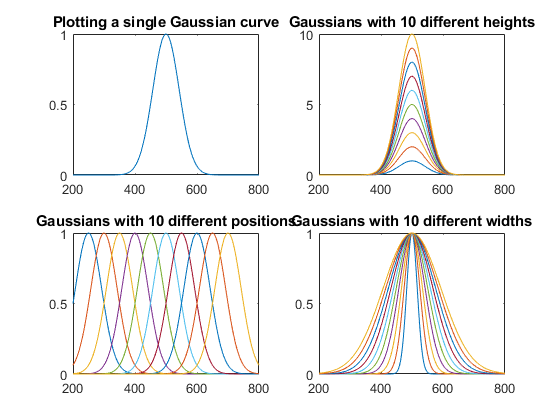
\includegraphics[width=1\textwidth]{image10.png}
    \end{minipage}\hfill
    \begin{minipage}{0.5\textwidth}
        \centering
        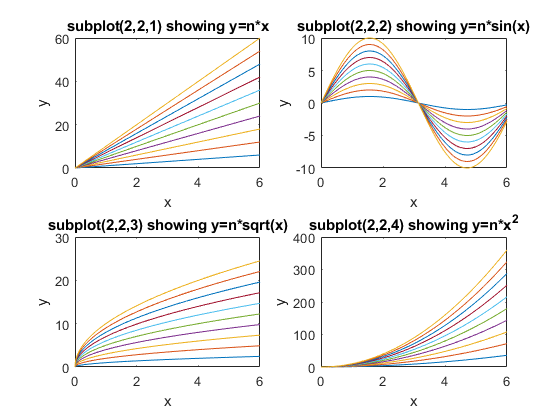
\includegraphics[width=1\textwidth]{image11.png}
    \end{minipage}
\end{figure}
\label{ref-0015}

La sottrazione di due segnali \texttt{\textbf{a}} e \texttt{\textbf{b}}, come a pagina \pageref{ref-0006}, si pu\`{o} eseguire semplicemente scrivendo \texttt{\textbf{a-b}}. Per disegnare la differenza, si scrive "\texttt{plot(a-b)}". Allo stesso modo, per disegnare il rapporto tra due segnali, come a pagina \pageref{ref-0007}, si scriver\`{a} "\texttt{plot(a./b)}". Quindi, "./" significa dividere punto-per-punto e ".*" significa moltiplicare punto-per-punto. Il * di per s\'{e} indica la moltiplicazione tra matrici, utilizzabile per eseguire moltiplicazioni ripetute senza usare i cicli. Per esempio, se x \`{e} un vettore.

 \texttt{A=[1:100]'*x}\texttt{;}

crea una matrice \textbf{A} in cui ciascuna colonna \`{e} x moltiplicato per i numeri 1, 2,...100. \`{E} equivalente, ma pi\`{u} compatto e pi\`{u} veloce, della scrittura di un ciclo "for" come questo:

\texttt{for n=1:100;}

\texttt{A(:,n)=n.*x;}

\texttt{end}

Vedere \href{https://terpconnect.umd.edu/~toh/spectrum/TimeTrial.txt}{TimeTrial.txt} per i dettagli. Sar\`{a} utile pre-allocare lo spazio di memoria per la matrice \textbf{A} aggiungendo l'istruzione \texttt{A=zeros(100,100)} prima del ciclo. Anche cos\`{i}, la notazione matriciale \`{e} pi\`{u} veloce del loop.

In Matlab/Octave, "/" non \`{e} lo stesso di "\textbackslash ". Digitando "b\textbackslash a" verr\`{a} calcolata la "\href{http://www.mathworks.com/help/matlab/ref/arithmeticoperators.html}{divisione matriciale a sinistra}", in pratica, il rapporto medio ponderato delle ampiezze dei due vettori (una specie di soluzione per l'approssimazione con i quadrati-minimi). Il punto qui \`{e} che \textit{Matlab non richiede di trattare vettori e matrici come raccolte di numeri}; sa quando si ha a che fare con le matrici o quando il risultato di un calcolo sar\`{a} una matrice e di conseguenza regola i calcoli. Cfr. \url{https://www.mathworks.com/help/matlab/matlab_prog/array-vs-matrix-operations.html}.

Probabilmente gli errori pi\`{u} comuni che si faranno in Matlab/Octave riguarderanno la punteggiatura, come il mischiare punti, virgole, due-punti e punti-e-virgola o parentesi, quadre e graffe; si pu\`{o} digitare "\href{https://terpconnect.umd.edu/~toh/spectrum/help\_punct.txt}{help punct}" al prompt di Matlab e \textit{leggere il file di help} fino allo sfinimento. \textit{Le piccole cose possono significare molto} in Matlab. Un altro errore comune \`{e} quello di confondere le righe e le colonne di vettori e matrici. (Una confessione: commetto \textit{ancora} questo tipo di errori). Ecco un \href{https://terpconnect.umd.edu/~toh/spectrum/RowsAndColumns.txt}{file di testo che fornisce esempi} di normali operazioni tra vettori e matrici e gli errori in Matlab e in Octave. Per i neofiti, si consiglia di leggere questo file e di provare gli esempi. Scrivere in Matlab \`{e} un processo per tentativi ed errori, con l'accento sull'\textit{errore}. Iniziare con cose semplici, farle funzionare e poi progredire.

\InsImage{1.0}{image12.png}\textit{Ci sono molti esempi di codice in questo testo da copiare, incollare e modificare sulla riga di comando di Matlab/ Octave}, ed \`{e} il miglior modo per imparare. Nella versione PDF di questo libro, si possono selezionare per poi copiare e incollare o selezionare e trascinare, esempi di codice su singola o pi\`{u} linee nell'editor di Matlab o di Octave o direttamente sulla riga di comando e poi premere \textbf{Enter} per eseguirle immediatamente). Ci\`{o} \`{e} particolarmente conveniente se si esegue Matlab e si legge dal sito web o dal libro sullo stesso computer; posizionare le finestre in modo che Matlab condivida lo schermo con questo sito web (p.es. Matlab a sinistra e il browser web a destra \href{https://terpconnect.umd.edu/~toh/spectrum/CopyPasteintoMatlab.png}{come mostrato sopra}). O, ancora meglio, si potrebbero avere \textit{due} monitor collegati allo stesso computer configurato in modo che espanda il desktop orizzontalmente.

Suggerimento: \textit{Se tentando di eseguire uno di questi script o funzione e si riceve l'errore "missing function", si cerchi l'elemento mancante in} \textit{\url{http://tinyurl.com/cey8rwh}}\textit{, scaricandolo nel proprio path e riprovare.}

Una cosa che si noter\`{a} in Matlab \`{e} che la \textit{primissima volta} che si esegue uno script o una funzione, e \textit{solo} la prima volta, c'\`{e} un piccolo ritardo prima dell'esecuzione, mentre Matlab compila il codice in linguaggio macchina. Questo, per\`{o}, avviene solo la \textit{prima} volta; dopo di ci\`{o}, l'esecuzione inizier\`{a} immediatamente. (Per un'esecuzione pi\`{u} veloce, \`{e} disponibile separatamente il ``\href{http://www.mathworks.com/products/matlab-compiler-sdk/index.html}{Matlab Compiler}'' che consente di condividere i programmi come applicazioni \textit{autonome}, separate dall'ambiente Matlab. ``\href{http://www.mathworks.com/products/matlab-compiler-sdk/index.html}{Matlab Compiler SDK}'' consente la creazione di librerie shared C/C++, assembly di Microsoft .NET, classi Java e pacchetti Python partendo dai programmi Matlab). Si pu\`{o} anche fare qualche disegno in \textit{real-time} in Matlab/Octave; cfr. pagina \pageref{ref-0418}.

\textbf{Inserimento dei dati in Matlab/Octave}\index{\textbf{Getting data into Matlab/Octave}}\textbf{.} Si possono \href{http://www.mathworks.com/help/matlab/import\_export/recommended-methods-for-importing-data.html}{importare i propri dati in Matlab} o in Octave utilizzando il comando ``load''. I dati si possono importare da file di testo (.txt), CSV (comma separated values), da diversi formati di immagini e suoni o da spreadsheet. Matlab ha anche un comodo \textit{Import Wizard} (cliccare su \textbf{File {\textgreater} Import Data}) che fornisce un'anteprima del file di dati, lo analizza cercando colonne e righe di dati numerici e le relative etichette dando la possibilit\`{a} di selezionare e ri-etichettare le variabili desiderate consentendo di importarli come vettori, matrici o tabelle. Utilissimo.

\InsImage{1.0}{ImportDataWizard.png}Si possono importare anche dati approssimativi provenienti da grafici e da quelli \textit{stampati} utilizzando la funzione interna "ginput" che ricava i dati numerici dalle coordinate dei click del mouse o utilizzando applicazioni come ``\href{https://datathief.org/}{\textit{Data Thief}}'' o \href{http://www.mathworks.com/matlabcentral/fileexchange/11077-figure-digitizer}{\textit{Figure Digitizer}} in the Matlab File Exchange.

Matlab versione R2013a o pi\`{u} recente pu\`{o} anche \href{http://blogs.mathworks.com/pick/2013/08/09/reading-from-sensors-on-your-mobile-phone/}{leggere dei sensori dal proprio telefono iPhone o Android }via Wi-Fi. Per leggere gli output da vecchi strumenti analogici, c'\`{e} bisogno di un \href{https://www.google.com/\#q=analog-to-digital+converter,}{convertitore analogico-digitale}, una \href{https://www.google.com/\#q=Arduino+microcontroller+board}{scheda col microcontroller Arduino} o un \href{https://www.google.com/\#q=USB+voltmeter}{voltmetro USB}.

\textbf{Versioni di Matlab}\index{\textbf{Matlab Versions}}. La versione standard \textit{commerciale} di Matlab \`{e} costosa (oltre \$2000) ma ci sono versioni \textit{student} e \textit{home} che costano molto meno (circa \$49 per una versione base per studenti) e che hanno tutte le capacit\`{a} di eseguire i metodi descritti in questo libro \textit{a velocit\`{a} di esecuzione comparabili}. \InsImageInline{0.8}{l}{image14.png}C'\`{e} anche \href{https://www.mathworks.com/products/matlab-online.html}{\textit{Matlab Online}}, che \textit{gira in un normale browser web} (vedere il grafico a pag. \pageref{ref-0002}). Non c'\`{e} nemmeno bisogno di un normale computer: c'\`{e} un'app \href{https://itunes.apple.com/us/app/matlab-mobile/id370976661?mt=8}{Matlab Mobile} gratuita che esegue un'interfaccia Matlab su iPhone e su iPad connessi a Internet (illustrati a lato). Richiede solo una licenza di base per studenti e utilizza tutte le funzioni standard, oltre a qualsiasi funzione o script del libro, o anche quelle scritte dagli utenti e precedentemente caricate nel proprio account sul \href{https://www.mathworks.com/cloud.html}{Matlab cloud}. Tutte queste versioni hanno una velocit\`{a} di calcolo sono per lo pi\`{u} entro un fattore 2 l'una dall'altra, come mostrato in \href{https://terpconnect.umd.edu/~toh/spectrum/TimeTrial.txt}{TimeTrial.txt}. Cfr. \url{https://www.mathworks.com/pricing-licensing.html}\uline{\textcolor{color-2}{.}}

\section{\href{http://en.wikipedia.org/wiki/GNU\_Octave}{\label{ref-0016}\label{ref-0017}GNU Octave}\label{ref-0018}}

\InsImage{1.0}{Octave.gif.png}
Octave\index{Octave} \`{e} una \href{https://cvw.cac.cornell.edu/matlab/octave}{alternativa gratuita a Matlab} che \`{e} "\href{http://en.wikipedia.org/wiki/GNU\_Octave\#MATLAB\_compatibility}{per lo pi\`{u} compatibile}". \href{http://www.dspguru.com/dsp/links/matlab-clones}{DspGURU} dice che Octave \`{e} ``...un clone maturo e di alta qualit\`{a} di Matlab. Ha il pi\`{u} alto grado di compatibilit\`{a} con Matlab tra tutti i cloni.'' Tutto quanto detto in precedenza su Matlab funziona anche in Octave. Infatti, \textit{le versioni pi\`{u} recenti di quasi tutte le funzioni, gli script, i demo e gli esempi in Matlab di questo documento funzioneranno con l'ultima versione di Octave senza modifiche.} Fanno eccezione le funzioni interattive a riga di comando \textit{iPeak} (pagina \pageref{ref-0320}), \textit{iSignal} (pagina \pageref{ref-0433}) e \textit{ipf.m} (pagina \pageref{ref-0461}); queste funzionano solo in Matlab. Se si prevede di utilizzare Octave, ci si assicuri di avere le versioni correnti; molte sono state aggiornate per avere la compatibilit\`{a} con Octave nel 2015 e questo \`{e} un progetto in corso. C'\`{e} una \href{http://wiki.octave.org/FAQ\#Porting\_programs\_from\_Matlab\_to\_Octave}{FAQ} che pu\`{o} aiutare nel \href{http://wiki.octave.org/FAQ\#Porting\_programs\_from\_Matlab\_to\_Octave}{porting di programmi Matlab in Octave}. Cfr. ``\href{https://www.google.com/search?q=Key+Differences+Between+Octave+\%26+Matlab&oq=Key+Differences+Between+Octave+\%26+Matlab&aqs=chrome..69i57j33i10i22i29i30.1334j0j4&sourceid=chrome&ie=UTF-8}{Differenze tra Octave \& Matlab}''. Ci sono versioni Windows, Mac e Unix di Octave. La versione Windows \`{e} scaricabile da \href{http://sourceforge.net/projects/octave/files/Octave\%20Windows\%20binaries/Octave\%203.6.1\%20for\%20Windows\%20MinGW\%20installer/}{Octave Forge}. Ci sono molti help online: Google "\href{https://www.google.com/search?q=GNU+Octave&aq=f&oq=GNU+Octave&sugexp=chrome,mod=0&sourceid=chrome&ie=UTF-8}{GNU Octave}" o si vedano i \href{http://www.youtube.com/results?search\_query=GNU+octave&oq=GNU+octave&gs\_l=youtube.3..0l2j0i5.18053.19469.0.20453.4.4.0.0.0.0.52.167.4.4.0...0.0...1ac.1.UrtIQXZNZoQ}{video YouTube} per un aiuto. Per le applicazioni specifiche al signal processing, su Google "\href{https://www.google.com/search?q=signal+processing+octave&ie=utf-8&oe=utf-8&aq=t&rls=org.mozilla:en-US:unofficial&client=seamonkey-a}{signal processing octave}".

\href{https://www.gnu.org/software/octave/news/release/2019/03/01/octave-5.1-released.html}{Octave Version 6.2.0} \`{e} ora disponibile per il \href{http://www.gnu.org/software/octave/download.html}{download}.La documentazione \`{e} online; vedere \url{https://www.octave.org}. Quasi tutti gli script e le funzioni girano su Octave. Tuttavia, \`{e} ancora computazionalmente circa 5 volte pi\`{u} lento, mediamente, rispetto all'ultima versione di Matlab, a seconda dell'attivit\`{a} (sono disponibili confronti specifici per diverse attivit\`{a} di signal processing in \href{https://terpconnect.umd.edu/~toh/spectrum/TimeTrial.txt}{TimeTrial.txt}). Conclusione: Matlab \`{e} migliore, ma se non \`{e} alla portata, Octave fornisce la maggior parte delle funzionalit\`{a} allo 0\% del costo. Nota: il pi\`{u} vecchio \href{http://wiki.octave.org/Rasperry\_Pi}{Octave 3.6 pu\`{o} funzionare anche su un Raspberry Pi} \textcolor{color-3}{(un computer a scheda singola a basso costo).}

\section{Spreadsheet o Matlab/Octave\index{Spreadsheet or Matlab/Octave}?\label{ref-0019}}

Per l'elaborazione dei segnali, Matlab/Octave \`{e} pi\`{u} veloce e potente rispetto all'utilizzo di uno spreadsheet, ma si pu\`{o} sicuramente dire che gli spreadsheet sono presenti pi\`{u} spesso di Matlab e di Octave sui computer dei tecnici. Per cominciare, gli spreadsheet sono economici, e pi\`{u} facili da usare, ed offrono una presentazione e un'interfaccia flessibile. I fogli di calcolo sono migliori per l'immissione manuale dei dati; si possono facilmente distribuire su dispositivi portatili come smartphone e tablet (p.es. utilizzando \textit{Google Sheets}, \href{https://www.apple.com/mac/numbers/}{i}\href{https://www.apple.com/mac/numbers/}{\textit{Cloud Numbers}} o l'app \href{https://itunes.apple.com/us/app/microsoft-excel-for-ipad/id586683407?mt=8}{\textit{Excel}}). \textit{Gli spreadsheet sono concreti e a pi\`{u} basso livello, mostrando ogni singolo valore esplicitamente in una cella.} Al contrario, \textit{Matlab}/\textit{Octave} \`{e} a pi\`{u} alto livello di astrattismo, dato che una singola variabile pu\`{o} essere un numero, un vettore o una matrice e ogni punteggiatura o funzione pu\`{o} fare molta differenza. \`{E} molto potente ma difficile da padroneggiare \textit{all'inizio}. Un vantaggio di Matlab e Octave \`{e} che i loro file di funzioni o script (``file m'') sono semplici file testo con l'estensione ``.m'', quindi \textit{questi file si possono aprire e controllare con qualsiasi editor di testi, anche sui dispositivi che non hanno Matlab o Octave installato}, il che facilita la traduzione degli script e delle funzioni in altri linguaggi. Inoltre, le funzioni definite dall'utente possono chiamare altre funzioni native o definite dall'utente, che a loro volta possono chiamare altre funzioni, e cos\`{i} via, consentendo la \textit{costruzione di funzioni di alto livello con strati molto complessi}. Fortunatamente, Matlab pu\`{o} facilmente analizzare file Excel .xls e .xlsx ed importarne le righe e le colonne in variabili vettoriali/matriciali.

Utilizzando l'analogia con i circuiti elettronici, gli spreadsheet sono come \textit{componenti discreti} elettronici, dove ogni resistore, condensatore, induttanza e transistor \`{e} un'entit\`{a} discreta e macroscopica direttamente visibile e manipolabile. Un linguaggio di programmazione basato su funzioni come Matlab/Octave \`{e} pi\`{u} simile alla \textit{micro-elettronica}, dove le funzioni (i "file-m" che iniziano con "function...") sono i "chip", che racchiudono complesse operazioni in un unico pacchetto \textit{con i pin di I/O documentati} (gli \textit{argomenti} di input e output delle funzioni) collegabili ad altre funzioni, ma che \textit{nascondono i dettagli interni} (a meno che non interessi guardare il codice, cosa che \`{e} sempre fattibile). Un buon esempio \`{e} il "timer 555", un timer, un generatore di impulsi ed un oscillatore ad 8-pin, introdotto nel 1972, usato ancora oggi diventando il \href{https://en.wikipedia.org/wiki/555\_timer\_IC}{circuito integrato pi\`{u} popolare mai prodotto}. Quasi tutta l'elettronica ora \`{e} fatta con i chip, perch\'{e} \textit{\`{e} pi\`{u} facile capire il numero relativamente basso di input e output} di un chip che avere a che fare col gran numero di componenti all'interno. Gran parte di Matlab/Octave \`{e} scritto in Matlab/Octave stesso, utilizzando funzioni pi\`{u} semplici per costruire quelle pi\`{u} complesse. Ci si possono scrivere nuove funzioni che estendono il linguaggio in qualsiasi direzione sia necessario (pagina \pageref{ref-0042}).

Alla fine si ha che gli spreadsheet sono pi\`{u} facili all'inizio, ma, dalla mia esperienza, alla fine l'approccio a Matlab/ Octave \`{e} pi\`{u} veloce, pu\`{o} gestire moli di dati maggiori ed \`{e} in definitiva pi\`{u} produttivo. Ci\`{o} \`{e} dimostrato dal confronto di entrambe le piattaforme per la \href{https://terpconnect.umd.edu/~toh/spectrum/CurveFittingB.html\#spreadsheets}{spettroscopia multicomponente} trattata a pagina \pageref{ref-0243} (\href{https://terpconnect.umd.edu/~toh/spectrum/RegressionDemo.xls}{RegressionDemo.}\uline{xls} rispetto a Matlab/Octave \href{https://terpconnect.umd.edu/~toh/spectrum/CLS.m}{CLS.m}). Ancora pi\`{u} drammatici sono i diversi approcci per trovare e misurare i picchi nei segnali, che vengono trattati nella sezione iniziale a pagina \pageref{ref-0294} (p.es. uno \href{https://terpconnect.umd.edu/~toh/spectrum/PeakDetectionAndMeasurement.xls}{spreadsheet da 250Kbyte} rispetto a uno \href{https://terpconnect.umd.edu/~toh/spectrum/findpeaks.m}{script Matlab da 7Kbyte} che fa la stessa cosa ma \`{e} \textit{50 volte pi\`{u} veloce}). Se si ha una grande mole di dati da trattare automaticamente con un processo personalizzato a pi\`{u} passi, senza intervento manuale e il pi\`{u} velocemente possibile, allora Matlab \`{e} ottimo\textit{.} \`{E} molto pi\`{u} semplice scrivere uno script in Matlab che \textit{automatizzer\`{a} l'elaborazione in autonomia di grossi volumi di dati} memorizzati in diversi file sul computer, come mostrato nell'esempio a pagina \pageref{ref-0413}.

Sia i programmi per spreadsheet che per Matlab/Octave hanno un enorme vantaggio sui programmi commerciali per utenti finali e i programmi compilati gratuitamente come SPECTRUM (pagina \pageref{ref-0481}); si possono \textit{ispezionare e modificare} per personalizzare le routine per esigenze specifiche. \`{E} facile apportare semplici modifiche con poca o nessuna conoscenza della programmazione. Per esempio, si possono facilmente modificare le etichette, i titoli, i colori o lo stile dei grafici - nei programmi Matlab o Octave, basta cercare "title(", "label(" o "plot(". Il codice contiene \textit{commenti che indicano i posti dove si possono fare specifiche modifiche}: basta usare \textbf{Find...} per cercare la parola "change". \textit{Si \`{e} invitati a modificare a piacimento gli script e le funzioni.} La \href{https://terpconnect.umd.edu/~toh/spectrum/license.txt}{licenza software} racchiusa nei commenti di tutto il mio codice Matlab/Octave \`{e} molto liberale.\label{ref-0020}

\chapter{Segnali e rumore\index{noise}\label{ref-0021}\label{ref-0022}\label{ref-0023}\label{ref-0024}}

Le misure sperimentali non sono sempre perfette, anche quando si usano strumenti moderni e sofisticati. Vengono riconosciuti due tipi principali di errori di misurazione: (a) \textit{errore sistematico}, in cui in ogni misura \`{e} costantemente inferiore o superiore al valore corretto di una certa percentuale o quantit\`{a}, e (b) \textit{errore casuale}, in cui ci sono variazioni imprevedibili nel segnale misurato da momento a momento o da misura a misura. Quest'ultimo tipo di errore \`{e} spesso chiamato \textit{rumore}, per analogia col rumore acustico. Ci sono molte sorgenti di rumore nelle misure fisiche, come vibrazioni strutturali, correnti d'aria, fluttuazioni della corrente, radiazioni vaganti emesse da dispositivi elettrici, elettricit\`{a} statica, interferenze da trasmissioni radio o TV, turbolenza nel flusso di gas o di liquidi, movimento termico casuale delle molecole, radiazione di fondo da elementi radioattivi naturali, "raggi cosmici" dallo spazio (sul serio), la stessa natura quantistica di base della materia e dell'energia e il \href{https://terpconnect.umd.edu/~toh/spectrum/CaseStudies.html\#Digitization}{rumore di digitalizzazione} (l'arrotondamento a un numero fisso di cifre). Poi, ovviamente, c'\`{e} l'onnipresente "errore umano", che pu\`{o} essere un fattore importante ogni volta che gli esseri umani sono coinvolti nel funzionamento, nella regolazione, nella registrazione, nella calibrazione o nel controllo degli strumenti e nella preparazione dei campioni per la misurazione. Se \`{e} presente un errore casuale, una serie di misure ripetute produrr\`{a} risultati che non sono tutti uguali ma piuttosto variano o si disperdono attorno a un \href{https://en.wikipedia.org/wiki/Average}{valore medio}, che \`{e} la somma dei valori divisa per il numero di valori "d": \texttt{sum(d)./length(d)} in notazione Matlab/Octave. Il modo pi\`{u} comune per misurare la quantit\`{a} di variazione o dispersione di un insieme di valori di dati consiste nel calcolare la \href{https://en.wikipedia.org/wiki/Standard\_deviation}{\textit{deviazione standard}}, che \`{e} la radice quadrata della somma dei quadrati della deviazione dalla media diviso il numero di punti meno uno: \texttt{sqrt(sum((d-mean(d)).\textasciicircum{}2)./ (length(d)-1))}. In notazione Matlab/Octave, viene pi\`{u} facilmente calcolata con la funzione nativa \texttt{std(d), dove d \`{e} il vettore dei dati}. Un fatto fondamentale delle variabili casuali \`{e} che quando si combinano, si devono calcolare i risultati \textit{statisticamente}. Ad esempio, quando vengono aggiunte due variabili casuali, la deviazione standard della somma \`{e} la "somma quadratica" (la radice quadrata della somma dei quadrati) delle deviazioni standard delle singole variabili, come dimostrato dalle serie di comandi di Matlab/Octave a \href{https://terpconnect.umd.edu/~toh/spectrum/RandomNoisesAddQuadratically.txt}{questo indirizzo}. Da provare.

Il termine ‘segnale’ ha due significati. In senso pi\`{u} generale, pu\`{o} significare l'\textit{intera} registrazione dei dati, incluso il rumore e altri artefatti, come nel ``segnale originale'' prima dell'applicazione dell'elaborazione. Ma pu\`{o} anche indicare solo la parte \textit{desiderabile} o \textit{importante} dei dati, il \textit{vero} \textit{segnale sottostante} che si cerca di misurare, come nell'espressione ``rapporto segnale-rumore''. Un problema fondamentale nella misura del segnale \`{e} distinguere il vero segnale dal rumore. Per esempio, si supponga di voler misurare la media del segnale in un certo tempo o l'altezza di un picco o l'area del picco che si ottiene dai dati. Nello spettro di assorbimento\index{absorption spectrum} sulla met\`{a} destra della figura a pagina \pageref{ref-0005}, le parti "importanti" sono probabilmente i picchi di assorbimento situati a 520 e a 550 nm. L'altezza o la posizione di uno di questi picchi potrebbe essere considerata il segnale, a seconda dell'applicazione. In questo esempio, l'altezza del picco pi\`{u} grande \`{e} di circa 0,08 unit\`{a} di assorbanza. Ma come misurare il rumore? Nel caso eccezionale che si abbia un sistema fisico \textit{e} uno strumento di misura, \textit{entrambi} completamente stabili (\textit{eccetto} per il rumore casuale), un modo semplice per isolare e misurare il rumore consiste nel \textit{registrare due segnali m1 ed m2 dello stesso sistema fisico}. Sottraendo queste due registrazioni, la parte del segnale verr\`{a} annullata. Quindi la deviazione standard del rumore nei segnali originali \`{e} data da sqrt((std(m1-m2)\textsuperscript{2})/2), dove ``sqrt'' \`{e} la radice quadrata e ``std'' \`{e} la deviazione standard. (La semplice derivazione di questa espressione si basa sulle \href{https://terpconnect.umd.edu/~toh/spectrum/Derivation.txt}{regole per la propagazione degli errori matematici} e viene elaborata in \url{https://terpconnect.umd.edu/~toh/spectrum/Derivation.txt}). Lo script Matlab/Octave ``\href{https://terpconnect.umd.edu/~toh/spectrum/SubtractTwoMeasurements.m}{SubtractTwoMeasurements.m}'' mostra questo processo quantitativamente e graficamente  (\uline{sotto})..

\InsImageInline{0.5}{r}{image15.png}Ma si supponga che le misure non siano cos\`{i} riproducibili o che si abbia solo \textit{una} delle registrazioni di questo spettro senza altri dati. In questo caso, si pu\`{o} tentare di stimare il rumore nel segnale registrato, basandosi sull'\textit{assunto} che le \textit{fluttuazioni a breve termine} visibili nel segnale - le piccole irregolarit\`{a} casuali sovrapposte al segnale regolare e fluido - siano \textit{rumore} e non parti del vero segnale sottostante. Ci\`{o} dipende da una certa conoscenza dell'origine del segnale e dalle possibili forme che potrebbe assumere. Gli esempi nella sezione precedente sono gli spettri di assorbimento di soluzioni liquide nell'intervallo di lunghezze d'onda da 450 nm a 700 nm (pagina \pageref{ref-0005}). Queste soluzioni normalmente mostrano picchi ampi e lisci con una larghezza tra i 10 e i 100 nm, quindi quelle piccole oscillazioni devono essere \textit{rumore}. In questo caso, tali fluttuazioni hanno una deviazione standard di circa 0.001. Spesso il modo migliore per misurare il rumore \`{e} individuare una regione sulla linea di base dove il segnale \`{e} piatto e qui calcolare la deviazione standard. Questo \`{e} facile da fare con un computer se il segnale \`{e} digitalizzato. La cosa importante \`{e} che si deve conoscere abbastanza sulla misurazione e i dati che genera per riconoscere i tipi di segnali riproducibili, in modo da avere la possibilit\`{a} di distinguere quale sia il \textit{segnale} e quale il \textit{rumore}.\label{ref-0025}

\`{E} importante comprendere che le deviazioni standard calcolate su un piccolo insieme di misure possono essere molto pi\`{u} alte o molto inferiori rispetto alla deviazione standard effettiva su un numero maggiore di misure. Per esempio, la funzione Matlab/Octave \texttt{randn(1,}\texttt{\textit{n}}\texttt{)}, dove \textit{n} \`{e} un intero, restituisce \textit{n} numeri casuali che hanno \textit{mediamente} una media di zero e una deviazione standard di 1.00 se \textit{n} \`{e} grande. Ma se \textit{n} \`{e} piccolo le deviazioni standard saranno diverse ogni volta che si esegue questa funzione; per esempio, se n=5, la deviazione standard \texttt{std(}\texttt{randn(1,5)}\texttt{)} pu\`{o} variare da 0.5 a 2 o anche pi\`{u}. Questa \`{e} la \href{https://en.wikipedia.org/wiki/Law\_of\_large\_numbers}{Legge dei Grandi Numeri}; \`{e} la natura inevitabile dei piccoli insiemi di numeri casuali che la loro deviazione standard sia solo una \textit{vaga approssimazione} della reale deviazione standard della ``popolazione'' in esame.

Un modo rapido ma approssimativo per stimare visivamente l'ampiezza del rumore \`{e} l'intervallo \textit{da-picco-a-picco}, che \`{e} la differenza tra i valori pi\`{u} alti e quelli pi\`{u} bassi tra due regioni in cui il segnale \`{e} piatto. L'intervallo picco-picco di \textit{n}=100 numeri casuali distribuiti normalmente \`{e} circa 5 volte la deviazione standard, come si pu\`{o} dimostrare eseguendo pi\`{u} volte questa riga di codice Matlab/Octave: \texttt{n=100; rn=randn(1,n);(max(rn)-min(rn))/std(rn)}. Per esempio, i dati nella met\`{a} destra della figura nella pagina successiva ha un picco al centro con un'altezza di circa 1.0. Anche il rumore da picco a picco sulla linea di base \`{e} di circa 1.0, quindi la deviazione standard del rumore \`{e} circa 1/5$^{\circ}$ di quello, o 0.2. \textit{Tuttavia, tale rapporto varia con il logaritmo di n} ed \`{e} pi\`{u} vicino a 3 quando \textit{n} = 10 ed a 9 quando \textit{n} = 100000. Al contrario, la deviazione standard diventa sempre pi\`{u} vicina al valore vero all'aumentare di \textit{n}. \`{E} meglio calcolare la deviazione standard, se possibile.

Oltre alla deviazione \textit{standard}, \`{e} anche possibile misurare (ma non usuale) la deviazione \textit{mediana assoluta} (mean absolute deviation "mad"). La deviazione standard \`{e} maggiore di quella mediana assoluta perch\'{e} quella standard pesa maggiormente le deviazioni pi\`{u} ampie. Per una variabile casuale normalmente distribuita, la deviazione mediana assoluta \`{e} in media l'80\% di quella standard: mad=0.8*std.

\InsImageInline{0.5}{r}{image16.png}La \textit{qualit\`{a}} di un segnale \`{e} spesso espressa quantitativamente come il \textit{rapporto} \textit{segnale-rumore} (S/N ratio o SNR), che \`{e} il rapporto dell'ampiezza dell'effettivo segnale (p.es. l'ampiezza media o l'altezza del picco) con la deviazione standard del rumore. Quindi il rapporto S/N dello spettro in figura a pagina \pageref{ref-0005} \`{e} circa $0.08/0.001 = 80$ ed il segnale a pagina \pageref{ref-0031} ha un rapporto S/N di $1.0/0.2 = 5$. Quindi diremmo che la qualit\`{a} del primo \`{e} migliore perch\'{e} ha un rapporto S/N maggiore. Misurare il rapporto S/N \`{e} molto facile se il rumore si pu\`{o} misurare separatamente, in assenza del segnale. A seconda del tipo di esperimento, \`{e} possibile acquisire letture del solo rumore, per esempio su un segmento della linea di base prima o dopo la presenza del segnale. Tuttavia, se l'ampiezza del rumore dipende dal livello del segnale, allora lo sperimentatore deve tentare di produrre un livello costante del segnale per consentire la misura del rumore sul segnale. In alcuni casi, \`{e} possibile utilizzare ``l'approssimazione dei minimi quadrati'' (pagina \pageref{ref-0258}) per approssimare accuratamente la forma del segnale mediante una funzione matematica (come una \href{https://terpconnect.umd.edu/~toh/spectrum/CurveFitting.html}{polinomiale} o la somma ponderata di un numero di semplici funzioni a \href{https://terpconnect.umd.edu/~toh/spectrum/CurveFittingC.html}{forma di picco}). Il rumore pu\`{o} quindi essere isolato sottraendo l'approssimazione dal segnale sperimentale senza smoothing. Per esempio, il grafico a lato, mostra un segnale sperimentale complesso che non arriva mai sulla linea di base per consentire una misura semplice del rumore.
 Ma il segnale pu\`{o} essere approssimato da un modello (la linea rossa) consistente in 5 funzioni di picchi Gaussiani con smoothing sovrapposti. La differenza tra i dati originali e il modello, mostrata in basso, \`{e} una buona misura del rumore casuale nei dati.

Se possibile, per\`{o}, \`{e} sempre meglio determinare la deviazione standard di misure ripetute di ci\`{o} che si vuol misurare (p.es. le altezze o le aree dei picchi o altro), anzich\'{e} cercare di stimare il rumore da una singola registrazione dei dati.\label{ref-0026}\label{ref-0027}

\section{\textbf{Il limite del rilevamento}\label{ref-0028}\label{ref-0029}}

\InsImageInline{0.5}{r}{RectSNRAtTheDetectionLimit.png}Il "limite del rilevamento" \`{e} definito come il segnale pi\`{u} piccolo che \`{e} possibile rilevare in modo affidabile in presenza di rumore. Nell'analisi quantitativa, \`{e} solitamente definito come la concentrazione che produce il pi\`{u} piccolo segnale rilevabile (Riferimento 92). Un segnale che sia al di sotto del limite di rilevamento non pu\`{o} essere rilevato in modo affidabile; ovvero, se la misura viene ripetuta, il segnale verr\`{a} spesso "perso nel rumore" e riportato come nullo. Un segnale al di sopra di tale limite verr\`{a} rilevato in modo affidabile e raramente, o mai, segnalato come nullo. Il valore pi\`{u} comune di rapporto segnale/rumore per un rilevamento affidabile \`{e} 3. Ci\`{o} \`{e} illustrato nella figura a lato (creata dallo script Matlab/Octave \href{https://terpconnect.umd.edu/~toh/spectrum/SNRdemo.m}{SNRdemo.m}). Questa figura mostra un segnale rumoroso sotto forma di un impulso rettangolare. Definiamo il "segnale" come l'ampiezza media del segnale durante l'impulso, indicato dalla linea rossa, che \`{e} circa 3. Definiamo il "rumore" come la deviazione standard del rumore casuale sulla linea di base prima e dopo l'impulso, che \`{e} circa 1.0, quasi 1/5 del rumore da picco a picco della linea di base (linee nere). Il rapporto segnale/rumore (SNR) in questo caso \`{e} circa 3, che \`{e} una definizione comune di limite di rilevamento. Ci\`{o} significa che i segnali inferiori a questo dovrebbero essere segnalati come "non rilevabili".

Ma c'\`{e} un problema. Il segnale qui \`{e} chiaramente rilevabile a occhio; infatti, dovrebbe essere possibile rilevare visivamente segnali pi\`{u} piccoli di questo. Come pu\`{o} essere? La risposta \`{e} "fare la media". Guardando questo segnale, si sta \textit{inconsciamente stimando la media dei punti} sull'impulso del segnale e sulla linea di base e la personale capacit\`{a} di rilevamento visivo viene migliorata da questa media. Senza tale media, guardando solo i \textit{singoli} punti nel segnale, all'incirca solo la met\`{a} di questi punti isolati soddisferebbe il criterio dell'SNR=3. Si pu\`{o} vedere, nel grafico precedente, che diversi punti sul picco del segnale sono un realt\`{a} \textit{pi\`{u} bassi} di alcuni punti sulla linea di base. Ma questo non \`{e} un problema nella pratica, perch\'{e} qualsiasi software scritto correttamente includer\`{a} la media che raddoppia la media visiva che tutti noi facciamo.

Nello script \href{https://terpconnect.umd.edu/~toh/spectrum/SNRdemo.m}{SNRdemo.m}, il numero di punti mediati \`{e} regolato dalla variabile "AveragePoints" \InsImageInline{0.5}{r}{RectSNR3.png} nella riga 7. Se lo si imposta a 5, il risultato (mostrato a lato) mostra che tutti i punti del segnale (ciascuno dei quali \`{e} ora la media di 5 punti originali) stanno al di sopra dei punti pi\`{u} alti della linea di base. Questo grafico rappresenta pi\`{u} da vicino ci\`{o} che giudichiamo quando guardiamo un segnale come quello nel grafico precedente, che ha una netta separazione tra il segnale e la linea di base. L'SNR del picco \`{e} migliorato da 3.1 a 7.7 e \textit{il limite di rilevamento si ridurr\`{a} di conseguenza}. Come regola pratica, per il tipo pi\`{u} comune di rumore, questo diminuisce all'incirca della radice quadrata del numero di punti mediati (sqrt(5)=2.2). Valori pi\`{u} alti miglioreranno ulteriormente l'SNR e ridurranno la deviazione standard relativa del segnale medio, ma il \textit{tempo di risposta} \textendash{} che \`{e} il tempo impiegato dal segnale per raggiungere il valore medio \textendash{} diventer\`{a} sempre pi\`{u} lento all'aumentare del numero di punti mediati. Ci\`{o} viene mostrato da \href{https://terpconnect.umd.edu/~toh/spectrum/RectSNR100pnts.png}{un altro grafico, con 100 punti mediati}. Con un segnale molto pi\`{u} basso pari a 1.0, il segnale originale \`{e} \href{https://terpconnect.umd.edu/~toh/spectrum/RectSNR1.png}{non rilevabile visivamente}, ma con una media di 100 punti, la \href{https://terpconnect.umd.edu/~toh/spectrum/RectSNR1avg100.png}{precisione del segnale \`{e} buona}; in questo caso la media digitale batte la media visiva. Si osserverebbe un comportamento simile se il segnale fosse un picco arrotondato anzich\'{e} un rettangolo.

In \href{https://terpconnect.umd.edu/~toh/spectrum/SNRdemo.m}{SNRdemo.m}, il rumore \`{e} costante e indipendente dall'ampiezza del segnale, che \`{e} il caso pi\`{u} comune. Nella variante \href{https://terpconnect.umd.edu/~toh/spectrum/SNRdemoHetero.m}{SNRdemoHetero.m}, il rumore nel segnale \`{e} direttamente proporzionale al livello del segnale o alla sua radice quadrata, di conseguenza il limite del rilevamento dipende dal rumore costante della linea di base (\href{https://terpconnect.umd.edu/~toh/spectrum/RectSNRhetero.png}{grafico}). Vedere pagina \pageref{ref-0036}. Nella variante \href{https://terpconnect.umd.edu/~toh/spectrum/SNRdemoArea.m}{SNRdemoArea.m}, \`{e} l'\textit{area} del picco che viene misurata anzich\'{e} la sua altezza, in cui si ottiene  un SNR migliorato della radice quadrata dell'ampiezza del picco (\href{https://terpconnect.umd.edu/~toh/spectrum/RectSNRarea.png}{grafico}).

Un esempio di applicazione pratica di un segnale come questo potrebbe essere quello dell'accensione di una spia o un cicalino se il segnale supera un valore di soglia di 1.5, per il segnale illustrato nelle figure sopra. Ci\`{o} non funzionerebbe se si usasse il segnale originale non mediato della figura precedente; non esiste un valore di soglia che non verrebbe mai superato dalla linea di base ma superato sempre dal segnale. Solo il segnale \textit{mediato} attiverebbe in modo affidabile l'allarme al di sopra della soglia di 1.5 e non lo attiverebbe mai al di sotto di 1.5.

Si sentir\`{a} anche il termine "Limite di determinazione", che \`{e} il segnale o la concentrazione pi\`{u} bassa che raggiunge una precisione minima accettabile, definita come la deviazione standard relativa dell'ampiezza del segnale. Il limite di determinazione viene definito con un rapporto segnale/rumore molto pi\`{u} alto, diciamo 10 o 20, a seconda dei requisiti delle proprie applicazioni. La media, come quella fatta qui, \`{e} la forma pi\`{u} semplice di "smoothing", che viene trattata nel prossimo capitolo (pagina \pageref{ref-0048}).

\section{Media di insieme\index{Ensemble averaging}\label{ref-0030}}

Una cosa fondamentale che distingue davvero il segnale dal rumore \`{e} che il rumore casuale non \`{e} lo stesso da una misura del segnale all'altra, mentre il vero segnale \`{e} (idealmente) riproducibile. Quindi, se il segnale pu\`{o} essere misurato pi\`{u} di una volta, si pu\`{o} usare questo fatto misurando il segnale pi\`{u} e pi\`{u} volte, il pi\`{u} velocemente possibile e \textit{sommando} tutte le misure punto per punto, e poi dividendo per il numero di segnali mediati. Questa \`{e} chiamata \textit{media d'insieme [ensemble averaging]} ed \`{e} uno dei metodi pi\`{u} potenti per migliorare i segnali, quando applicabile. Affinch\'{e} funzioni correttamente, il rumore deve essere casuale ed il segnale deve avvenire nello stesso tempo per ogni ripetizione. Si osservi l'esempio in figura.


\begin{center}
\InsImage{1.0}{Figure3.GIF.png}\label{ref-0031}
\end{center}



\begin{center}
\textit{In Window 1 (a sinistra) c'\`{e} una singola misura del segnale molto rumoroso. C'\`{e} un ampio picco al centro del segnale, ma \`{e} difficile misurarne la posizione, la larghezza e l'altezza in modo accurato perch\'{e} il rapporto S/N \`{e} pessimo. In Window 2 (a destra) c'\`{e} la media di 9 misure ripetute del segnale, mostra chiaramente il picco emergente dal rumore. Il miglioramento atteso nel rapporto S/N \`{e} 3 (la radice quadrata di 9). Spesso \`{e} possibile mediare centinaia di misure, ottenendo un miglioramento molto pi\`{u} sostanziale. Il rapporto S/N nel segnale medio risultante nell'esempio \`{e} circa 5.}
\end{center}


\`{E} possibile ridurre il rumore della digitalizzazione facendo la media d'insieme, \textit{ma solo se sono presenti, o aggiunte, piccole quantit\`{a} di rumore casuale al segnale}; cfr. pagina \pageref{ref-0366}. Lo script Matlab/Octave \href{https://terpconnect.umd.edu/~toh/spectrum/EnsembleAverageDemo.m}{EnsembleAverageDemo.m} dimostra graficamente la tecnica. (Se si sta leggendo online, \href{https://terpconnect.umd.edu/~toh/spectrum/EnsembleAverageDemo.png}{click qui per il grafico}\uline{)}. Altri esempi vengono mostrati nei link di queste animazioni video, \href{https://terpconnect.umd.edu/~toh/spectrum/EnsembleAverage1.wmv}{EnsembleAverage1.wmv} o \href{https://terpconnect.umd.edu/~toh/spectrum/EnsembleAverageDemo.gif}{EnsembleAverageDemo.gif}, che mostrano la media d'insieme di 1000 ripetizioni di un segnale, migliorando il rapporto S/N di circa 30 volte.

\textbf{Animazione visuale di una media di insieme.} Questi 17 secondi di filmato (\href{https://terpconnect.umd.edu/~toh/spectrum/EnsembleAverage1.wmv}{EnsembleAverage1.wmv}) mostrano la "ensemble averaging" di 1000 ripetizioni di un segnale con un pessimo rapporto S/N. Il segnale di per s\'{e} consiste in tre picchi posizionati a x = 50, 100 e 150, con altezze di 1, 2 e 3 unit\`{a}. I picchi del segnale sono sepolti nel rumore casuale la cui deviazione standard \`{e} 10. Pertanto, il rapporto S/N del picco pi\`{u} piccolo \`{e} 0.1, che \`{e} troppo basso per essere persino \textit{visto} come segnale e tanto meno per essere misurato. Il video mostra il segnale medio accumulato mentre si eseguono 1000 misure. Alla fine, il rumore si riduce (in media) della radice quadrata di 1000 (circa 32), in modo che il rapporto S/N dei picchi pi\`{u} piccoli finisca per essere di circa 3, quanto basta per rilevarne affidabilmente la presenza. Se si sta leggendo online, click \href{https://terpconnect.umd.edu/~toh/spectrum/EnsembleAverage1.wmv}{qui }per scaricare un breve video (2 MByte) in formato WMV.

\section{Distribuzione in frequenza del rumore casuale\index{Frequency distribution of random noise}\label{ref-0032}\label{ref-0033}}

\InsImageInline{0.5}{r}{image19.png}Talvolta il segnale e il rumore possono essere parzialmente distinti in base alle \href{https://terpconnect.umd.edu/~toh/spectrum/HarmonicAnalysis.html}{componenti in frequenza}: per esempio, il segnale pu\`{o} contenere soprattutto parti a bassa frequenza e il rumore pu\`{o} essere localizzato a frequenze pi\`{u} alte o distribuito su una gamma molto pi\`{u} ampia di frequenze. Questa \`{e} la base del \href{https://terpconnect.umd.edu/~toh/spectrum/FourierFilter.html}{filtraggio} e dello \href{https://terpconnect.umd.edu/~toh/spectrum/Smoothing.html}{smoothing} (pagina \pageref{ref-0045}). Nella figura a lato, il picco stesso contiene principalmente componenti a bassa frequenza, mentre il rumore \`{e} (apparentemente) casuale e distribuito su una gamma molto pi\`{u} ampia di frequenze. La frequenza del rumore \`{e} caratterizzata dal suo \href{http://en.wikipedia.org/wiki/Frequency\_spectrum}{spettro delle frequenze}, spesso descritto in termini di \href{http://en.wikipedia.org/wiki/Colors\_of\_noise}{colore del rumore}. Il \href{http://en.wikipedia.org/wiki/White\_noise}{\textit{rumore bianco}} \`{e} casuale ed ha \href{https://terpconnect.umd.edu/~toh/spectrum/WhiteNoiseSpectrum.png}{la stessa potenza su tutta la gamma di frequenze}. Il suo nome deriva dalla \textit{luce bianca}, che ha la stessa luminosit\`{a} a tutte le lunghezze d'onda nella regione del visibile. Il rumore nei segnali dell'esempio precedente, e nella met\`{a} sinistra della figura, \`{e} \textit{bianco}. Nel campo acustico, il rumore bianco suona come un \textit{sibilo}. Nelle misure scientifiche, il rumore bianco \`{e} molto comune. Ad esempio, il rumore di quantizzazione, il rumore di \href{http://en.wikipedia.org/wiki/Johnson–Nyquist\_noise}{Johnson-Nyquist} (termico), il \href{http://en.wikipedia.org/wiki/Photon\_noise}{rumore fotonico} e il rumore prodotto da \href{https://terpconnect.umd.edu/~toh/spectrum/CaseStudies.html\#G}{singoli spike} hanno tutti una distribuzione in frequenza bianca, ed hanno tutti in comune la loro origine in eventi istantanei quantizzati in discreto, come il flusso dei singoli elettroni e fotoni.

\InsImageInline{0.5}{r}{image20.png}Un rumore che ha un carattere pi\`{u} evidente alle basse frequenze, cio\`{e} che ha pi\`{u} potenza alle basse frequenze anzich\'{e} alle alte, \`{e} spesso chiamato "\href{http://en.wikipedia.org/wiki/Pink\_noise}{rumore rosa}". Nel campo acustico, il rumore rosa suona come un \textit{ruggito}. (Una sotto-specie frequente di rumore rosa \`{e} il "\href{https://www.google.com/search?ix=aca&sourceid=chrome&ie=UTF-8&q=1\%2Ff+noise}{rumore 1/f}", dove la potenza del rumore \`{e} inversamente proporzionale alla frequenza, illustrata nel quadrante in alto a destra della figura a lato). Il rumore rosa \`{e} pi\`{u} fastidioso del rumore bianco perch\'{e} una \textit{data deviazione standard del rumore rosa ha un maggior effetto sull'accuratezza della misura rispetto alla stessa deviazione standard del rumore bianco} (come dimostrato dalla funzione Matlab/Octave \href{https://terpconnect.umd.edu/~toh/spectrum/noisetest.m}{noisetest.m}, che genera la figura a lato). Inoltre, l'applicazione dello \href{https://terpconnect.umd.edu/~toh/spectrum/Smoothing.html}{smoothing} e del \href{https://terpconnect.umd.edu/~toh/spectrum/FourierFilter.html}{filtro} passa-basso (pagina \pageref{ref-0045}) per ridurre il rumore, \`{e} pi\`{u} efficace per il rumore bianco che per quello rosa. Quando \`{e} presente il rumore rosa, a volte \`{e} utile applicare delle tecniche di modulazione, per esempio, \href{http://en.wikipedia.org/wiki/Optical\_chopper}{il "chopping" ottico} o la \href{https://www.google.com/search?aq=f&ix=aca&sourceid=chrome&ie=UTF-8&q=wavelength+modulation}{modulazione a lunghezza d'onda} nelle misure ottiche, per convertire i segnali in corrente continua (DC) in segnali in corrente alternata (AC), aumentando cos\`{i} la frequenza del segnale verso una regione delle frequenze dove il rumore \`{e} pi\`{u} basso. In tali casi, si \`{e} soliti utilizzare un \href{http://terpconnect.umd.edu/~toh/models/lockin.html}{amplificatore lock-in}, o il suo equivalente digitale, per misurare l'ampiezza del segnale. Un altro tipo di rumore misurato a bassa frequenza \`{e} il rumore \href{https://en.wikipedia.org/wiki/Brownian\_motion}{\textit{browniano}}, dal nome del botanico Robert Brown. Viene anche chiamato "rumore rosso" [o marrone], per analogia con il rumore rosa, o "\href{https://en.wikipedia.org/wiki/Random\_walk}{passeggiata aleatoria}", ed ha una potenza \href{https://terpconnect.umd.edu/~toh/spectrum/RandomWalkFrequencySpectrum.png}{inversamente proporzionale al \textit{quadrato} della frequenza}. Questo tipo di rumore non \`{e} raro nei segnali sperimentali e pu\`{o} interferire seriamente con l'accuratezza delle misure. Vedere pagina \pageref{ref-0379}: \textit{Passeggiate aleatorie [Random walks] e correzione della linea di base}.

Al contrario, il rumore che ha pi\`{u} potenza alle frequenze \textit{alte} \`{e} detto \href{http://www.livescience.com/38583-what-is-blue-noise.html}{rumore ``blu''}. Questo tipo di rumore si incontra meno spesso nel lavoro sperimentale, ma pu\`{o} verificarsi in segnali elaborati che sono stati soggetti a una sorta di processo di \href{https://terpconnect.umd.edu/~toh/spectrum/Differentiation.html}{differenziazione} (pagina \pageref{ref-0081}) o che sono stati \href{https://terpconnect.umd.edu/~toh/spectrum/Deconvolution.html}{deconvoluti} da un processo di [blurring] o di ampliamento (pagina \pageref{ref-0152}). Il rumore blu \`{e} \textit{pi\`{u} facile} da ridurre con lo smoothing (pagina \pageref{ref-0032}) e ha un effetto minore sulle approssimazione dei minimi quadrati rispetto alla quantit\`{a} equivalente di rumore bianco.

\section{Dipendenza dall'ampiezza del segnale\index{Dependence on signal amplitude}\label{ref-0034}\label{ref-0035}\label{ref-0036}}

\InsImageInline{0.5}{r}{image21.png}Il rumore pu\`{o} anche essere caratterizzato dal modo in cui varia con l'ampiezza del segnale. Il rumore costante di ``sottofondo'' \`{e} indipendente dall'ampiezza del segnale. D'altro canto il rumore pu\`{o} aumentare con l'ampiezza del segnale, che \`{e} un comportamento spesso osservato nella spettroscopia di emissione, nella \href{https://www.chem.agilent.com/Library/technicaloverviews/Public/5990-7651EN.pdf}{spettroscopia di massa} e nello \href{http://terpconnect.umd.edu/~toh/spectrum/CaseStudies.html\#F}{spettro in frequenza dei segnali}. I nomi fantasiosi per questi due tipi di comportamenti sono rispettivamente \textit{Omoschedastico} e \textit{Eteroschedastico}, rispettivamente. Un modo per osservarlo consiste nel selezionare un segmento di segnale in cui l'ampiezza del segnale varia molto, approssimare il segnale a un \href{https://terpconnect.umd.edu/~toh/spectrum/CurveFitting.html}{polinomio}, o a un modello a picchi multipli (pagina \pageref{ref-0263}), e osservare come i residui variano con l'ampiezza del segnale. \href{https://terpconnect.umd.edu/~toh/spectrum/PropNoise.png}{L'esempio} a lato \`{e} un segnale sperimentale reale che mostra i residui di un'operazione di approssimazione della curva (pagina \pageref{ref-0258}) che evidenzia il rumore che aumenta con l'ampiezza del segnale. In altri casi, il rumore \`{e} quasi indipendente dall'ampiezza del segnale.

Spesso c'\`{e} un mix di rumori con comportamenti diversi; nella \href{http://www.agilent.com/labs/features/2011\_101\_spectroscopy.pdf}{spettroscopia ottica}, si riconoscono tre tipi diversi di rumore, basati sulla loro origine e su come variano con l'intensit\`{a} della luce: \textit{rumore fotonico}, \textit{rumore del rilevatore} e \textit{rumore di sfarfallio [flicker] (fluttuazione)}. Il rumore fotonico (spesso il rumore limitante negli strumenti che usano rilevatori con foto-moltiplicatori) \`{e} \textit{bianco} ed \`{e} proporzionale alla \textit{radice quadrata} dell'intensit\`{a} della luce. Il rumore del rilevatore (spesso il rumore limite negli strumenti che utilizzano rivelatori a fotodiodi a stato solido) \`{e} \textit{indipendente} dall'intensit\`{a} della luce e quindi l'SNR \`{e} direttamente proporzionale all'intensit\`{a} della luce. Il rumore da sfarfallio [flicker], provocato dall'instabilit\`{a} della sorgente di luce, vibrazioni, errori di posizionamento della cella campione, turbolenza del campione, dispersione della luce per delle particelle sospese, polvere, bolle, ecc., \`{e} direttamente proporzionale all'intensit\`{a} della luce (e solitamente \`{e} \textit{rosa} anzich\'{e} \textit{bianco}), quindi il rapporto S/N dello sfarfallio non diminuisce aumentando l'intensit\`{a} della luce. In pratica, \`{e} probabile che il rumore totale osservato sia un contributo di tutti e tre i tipi di dipendenza dall'ampiezza, nonch\'{e} un misto di rumori bianchi e rosa.

Solo in pochissimi casi speciali \`{e} possibile eliminare completamente il rumore, quindi di solito bisogna accontentarsi aumentando il pi\`{u} possibile il rapporto S/N. La soluzione, in qualsiasi sistema sperimentale consiste nel capire le possibili fonti del rumore, suddividere il sistema nelle sue parti e misurare il rumore generato in ognuna di esse, separatamente, per poi cercare di ridurre o compensare il pi\`{u} possibile ciascuna sorgente di rumore. Ad esempio, nella spettroscopia ottica, il rumore da sfarfallio della sorgente pu\`{o} essere spesso ridotto o eliminato utilizzando la stabilizzazione con \href{http://en.wikipedia.org/wiki/Feedback}{feedback}, scegliendo una sorgente di luce migliore, utilizzando un campione \href{http://en.wikipedia.org/wiki/Internal\_standard}{standard interno} o usando un tipo di strumento appositamente progettato come quelli a \href{https://terpconnect.umd.edu/~toh/models/UVVisSNR.html}{doppio-fascio [double-beam]}, a \href{https://terpconnect.umd.edu/~toh/models/DualWave1.html}{doppia lunghezza d'onda}, \href{https://terpconnect.umd.edu/~toh/spectrum/Differentiation.html}{derivativo} o a \href{https://terpconnect.umd.edu/~toh/modspec.html}{modulazione della lunghezza d'onda} (pagina \pageref{ref-0384}). L'effetto del rumore fotonico e di quello del rilevatore si possono ridurre aumentando l'intensit\`{a} della luce al rilevatore, e il rumore elettronico si pu\`{o} talvolta ridurre raffreddando o migliorando il rilevatore e/o l'elettronica. Il \href{http://en.wikipedia.org/wiki/Fixed-pattern\_noise}{rumore a schema fisso}, negli array di rilevatori, si pu\`{o} correggere via software. Solo il \textit{rumore fotonico} pu\`{o} essere previsto dai primi principi (p.es. come viene fatto in questi fogli di calcolo che simulano il comportamento segnale-rumore della \href{https://terpconnect.umd.edu/~toh/models/UVVisSNR.html}{spettrofotometria ultravioletta-visibile}, della \href{https://terpconnect.umd.edu/~toh/models/FluorescenceSNR.html}{spettrofotometria di fluorescenza} e della \href{https://terpconnect.umd.edu/~toh/models/AES.html}{spettrofotometria della emissione atomica}).

\section{La distribuzione di probabilit\`{a} del rumore casuale\index{Probability distribution of random noise}\label{ref-0037}}

\InsImageInline{0.5}{r}{CentralLimitDemo.gif.png}Un'altra propriet\`{a} che distingue il rumore casuale \`{e} la sua \href{http://en.wikipedia.org/wiki/Probability\_distribution}{distribuzione di probabilit\`{a}}, la funzione che descrive la probabilit\`{a} che una variabile casuale rientri in un certo intervallo di valori. Nelle misure fisiche, la distribuzione pi\`{u} comune \`{e} chiamata \href{http://en.wikipedia.org/wiki/Normal\_distribution}{\textit{curva normale}} (detta anche curva a ``campana'' o a ``pagliaio'') ed \`{e} descritta da una funzione \href{http://en.wikipedia.org/wiki/Gaussian\_function}{\textit{Gaussiana}}, \href{http://www.wolframalpha.com/input/?i=plot+y\%3Dexp\%28-\%28\%28x-mu\%29\%2F\%28sigma\%2F\%282*sqrt\%28ln\%282\%29\%29\%29\%29\%29\%5e2\%29+for+mu\%3D0\%2Csigma\%3D1}{y=e\textasciicircum{}(-(x-}\href{http://www.wolframalpha.com/input/?i=plot+y\%3Dexp\%28-\%28\%28x-mu\%29\%2F\%28sigma\%2F\%282*sqrt\%28ln\%282\%29\%29\%29\%29\%29\%5e2\%29+for+mu\%3D0\%2Csigma\%3D1}{\textit{mu}}\href{http://www.wolframalpha.com/input/?i=plot+y\%3Dexp\%28-\%28\%28x-mu\%29\%2F\%28sigma\%2F\%282*sqrt\%28ln\%282\%29\%29\%29\%29\%29\%5e2\%29+for+mu\%3D0\%2Csigma\%3D1}{)\textasciicircum{}2 / (2*}\href{http://www.wolframalpha.com/input/?i=plot+y\%3Dexp\%28-\%28\%28x-mu\%29\%2F\%28sigma\%2F\%282*sqrt\%28ln\%282\%29\%29\%29\%29\%29\%5e2\%29+for+mu\%3D0\%2Csigma\%3D1}{\textit{sigma}}\href{http://www.wolframalpha.com/input/?i=plot+y\%3Dexp\%28-\%28\%28x-mu\%29\%2F\%28sigma\%2F\%282*sqrt\%28ln\%282\%29\%29\%29\%29\%29\%5e2\%29+for+mu\%3D0\%2Csigma\%3D1}{\textasciicircum{}2)) / (sqrt(2*}\href{http://www.wolframalpha.com/input/?i=plot+y\%3Dexp\%28-\%28\%28x-mu\%29\%2F\%28sigma\%2F\%282*sqrt\%28ln\%282\%29\%29\%29\%29\%29\%5e2\%29+for+mu\%3D0\%2Csigma\%3D1}{\textit{mu}}\href{http://www.wolframalpha.com/input/?i=plot+y\%3Dexp\%28-\%28\%28x-mu\%29\%2F\%28sigma\%2F\%282*sqrt\%28ln\%282\%29\%29\%29\%29\%29\%5e2\%29+for+mu\%3D0\%2Csigma\%3D1}{)}\href{http://www.wolframalpha.com/input/?i=plot+y\%3Dexp\%28-\%28\%28x-mu\%29\%2F\%28sigma\%2F\%282*sqrt\%28ln\%282\%29\%29\%29\%29\%29\%5e2\%29+for+mu\%3D0\%2Csigma\%3D1}{\textit{*sigma}}\href{http://www.wolframalpha.com/input/?i=plot+y\%3Dexp\%28-\%28\%28x-mu\%29\%2F\%28sigma\%2F\%282*sqrt\%28ln\%282\%29\%29\%29\%29\%29\%5e2\%29+for+mu\%3D0\%2Csigma\%3D1}{)}, dove \textit{mu} \`{e} il valore medio (media) e \textit{sigma (}${\upsigma}$) \`{e} la deviazione standard. In questa distribuzione, gli errori di rumore pi\`{u} comuni sono piccoli (cio\`{e} vicini alla \textit{media}) e gli errori diventano meno comuni quanto maggiore \`{e} la loro deviazione dalla media. Allora perch\'{e} questa distribuzione \`{e} cos\`{i} comune? Il rumore osservato nelle misure fisiche \`{e} spesso la somma bilanciata di molti eventi casuali non osservati, ognuno dei quali ha una distribuzione di probabilit\`{a} sconosciuta, per esempio, alle propriet\`{a} cinetiche di gas o liquidi o al comportamento quantistico di particelle fondamentali come fotoni o elettroni. Ma quando molti di questi eventi si combinano per formare la variabilit\`{a} complessiva di una quantit\`{a} osservata, la distribuzione di probabilit\`{a} risultante \`{e} quasi sempre \textit{normale}, ovvero, descritta da una funzione Gaussiana. Questa comune osservazione \`{e} riassunta nel \href{http://en.wikipedia.org/wiki/Normal\_distribution\#Central\_limit\_theorem}{\textit{Teorema centrale del limite}}.

Una simulazione pu\`{o} dimostrare come questo comportamento si manifesti naturalmente. Nell'esempio a lato si comincia con un gruppo di 100.000 numeri casuali \textit{uniformemente distribuiti} che hanno la stessa probabilit\`{a} di avere un dato valore entro certi limiti, tra 0 e +1, in questo caso (come la funzione "rand" nella maggior parte degli spreadsheet e in Matlab/Octave). Il grafico in alto a sinistra della figura mostra la distribuzione di probabilit\`{a}, detta ``\href{http://en.wikipedia.org/wiki/Histogram}{istogramma}'', di quella variabile casuale. Successivamente, si combinano due set di tali variabili casuali indipendenti e uniformemente distribuite (cambiando i segni in modo che la media rimanga centrata sullo zero). Il risultato (mostrato nel grafico in alto a destra nella figura) ha una distribuzione \textit{triangolare} tra -1 e +1, col punto pi\`{u} alto a zero, perch\'{e} ci sono molti modi per far s\`{i} che la differenza tra due numeri casuali sia piccola, ma un solo modo affinch\'{e} la differenza sia 1 o -1 (ci\`{o} capita solo se un numero \`{e} esattamente zero \textit{e} l'altro \`{e} esattamente 1). In seguito, si combinano \textit{quattro} variabili casuali indipendenti (in basso a sinistra); la distribuzione risultante ha un intervallo totale da -2 a +2, ma \`{e} anche ancora \textit{meno} probabile che il risultato sia prossimo a 2 o a -2 e molti \textit{pi\`{u}} modi che portino il risultato ad essere piccolo, quindi la distribuzione \`{e} pi\`{u} stretta e pi\`{u} arrotondata, e sta gi\`{a} iniziando ad assomigliare alla distribuzione normale Gaussiana (generata utilizzando la funzione ``randn'' e mostrata per riferimento in basso a destra). Se si combinano sempre pi\`{u} variabili casuali uniformi e indipendenti, la distribuzione di probabilit\`{a} combinata si approssima sempre di pi\`{u} alla Gaussiana (mostrata per confronto in basso a destra). \textit{La distribuzione Gaussiana emergente che si osserva qui non \`{e} forzata da ipotesi precedenti; sorge naturalmente}. (Si pu\`{o} scaricare uno script Matlab per questa simulazione da \href{https://terpconnect.umd.edu/~toh/spectrum/CentralLimitDemo.m}{http://terpconnect.umd.edu/\textasciitilde{}toh/spectrum/CentralLimitDemo.m}\uline{)}.

Sorprendentemente, \textit{le distribuzioni dei singoli eventi non contano affatto}. Si possono modificare le singole distribuzioni in questa simulazione, sostituendo la funzione \textit{rand} con versioni modificate come sqrt(rand), sin(rand), rand\textasciicircum{}2, log(rand), ecc., per ottenere altre singole distribuzioni \textit{radicalmente non normali}. Ma sembra che non importa quale sia la distribuzione della singola variabile casuale, nel momento in cui si combinano anche solo quattro di esse, la distribuzione risultante \`{e} gi\`{a} visivamente vicina alla normale. Le osservazioni macroscopiche del mondo reale sono spesso il risultato di \textit{migliaia} o \textit{milioni} di singoli eventi microscopici, quindi qualunque sia la distribuzione di probabilit\`{a} dei \textit{singoli} eventi, le osservazioni macroscopiche \textit{combinate} si avvicinano a una distribuzione normale quasi perfettamente. \`{E} su questa comune aderenza alle distribuzioni normali che si basano le comuni procedure statistiche; l'uso della \href{http://en.wikipedia.org/wiki/Mean}{media}, della \href{http://en.wikipedia.org/wiki/Standard\_deviation}{deviazione standard} ${\upsigma}$, delle approssimazione \href{http://en.wikipedia.org/wiki/Least\_squares}{dei minimi quadrati}, degli \href{http://en.wikipedia.org/wiki/Confidence\_limits}{intervalli di confidenza}, ecc., sono tutti basati sull'\textit{assunzione} di una distribuzione normale.

Anche cos\`{i}, gli errori sperimentali e il rumore non sono \textit{sempre} normali; a volte ci sono errori molto grandi che cadono ben oltre il range ``normale''. Sono detti "valori anomali" e possono avere un grande effetto sulla deviazione standard. In questi casi, \`{e} possibile utilizzare lo ``\href{https://en.wikipedia.org/wiki/Interquartile\_range}{scarto interquartile}'' (IQR), definito come la differenza tra i quartili superiore e inferiore, invece della deviazione standard, perch\'{e} \textit{lo scarto interquartile non \`{e} influenzato da qualche valore anomalo}. Per una distribuzione \textit{normale}, lo scarto interquartile \`{e} pari a 1.34896 volte la deviazione standard. Un modo rapido per verificare la distribuzione di un ampio insieme di numeri casuali \`{e} calcolare sia la deviazione standard che lo scarto interquartile; se sono pi\`{u} o meno uguali, la distribuzione \`{e} probabilmente normale; se la deviazione standard \`{e} \textit{molto} pi\`{u} ampia, l'insieme dei dati probabilmente contiene valori anomali e la deviazione standard \textit{senza} i valori anomali si pu\`{o} stimare meglio dividendo lo scarto interquartile per 1.34896.

\textbf{L'importanza della distribuzione normale} sta nel fatto che se si conosce la deviazione standard ``${\upsigma}$'' di un valore misurato, si pu\`{o} prevedere che la sua misura possa essere errata di una certa quantit\`{a}. Circa il 68\% dei valori ricavati da una distribuzione normale sono entro un ${\upsigma}$ di distanza dalla media; il 95\% dei valori si trova entro 2${\upsigma}$, e il 99.7\% entro 3${\upsigma}$. Questa \`{e} nota come la \href{https://en.wikipedia.org/wiki/Normal\_distribution\#Standard\_deviation\_and\_coverage}{regola 3-sigma}. Ma il vero problema pratico \`{e} questo: le deviazioni standard: \textit{le deviazioni standard sono difficili da misurare con precisione a meno che non si disponga di un numero elevato di campioni.} Vedere ``\textit{La Legge dei Grandi Numeri''} (\uline{pagina} \pageref{ref-0425}\uline{).}\label{ref-0038}

Le tre caratteristiche del rumore discusse nei paragrafi precedenti - la distribuzione della frequenza, la distribuzione dell'ampiezza e la dipendenza dal segnale - sono reciprocamente indipendenti; in linea di principio un rumore pu\`{o} avere qualsiasi combinazione di queste propriet\`{a}.

\href{https://terpconnect.umd.edu/~toh/spectrum/SPECTRUM.html}{\textbf{SPECTRUM},} l'applicazione Macintosh freeware per il signal-processing, include diverse funzioni per misurare i segnali e il rumore nei men\`{u} \href{https://terpconnect.umd.edu/~toh/spectrum/~toh/spectrum/SPECTRUMReferenceManual.pdf\#page=9}{\textbf{Math}}e \href{https://terpconnect.umd.edu/~toh/spectrum/~toh/spectrum/SPECTRUMReferenceManual.pdf\#page=9}{\textbf{Window}}, pi\`{u} un generatore di segnali utilizzabile per generare segnali artificiali con bande Gaussiane e Lorentziane, onde sinusoidali e rumore casuale normalmente-distribuito nella voce \textbf{New} del men\`{u} \href{https://terpconnect.umd.edu/~toh/spectrum/~toh/spectrum/SPECTRUMReferenceManual.pdf}{\textbf{File}}. Vedere pagina \pageref{ref-0482}.

\section{Spreadsheet (Fogli di calcolo)\label{ref-0039}}

Gli spreadsheet popolari\textbf{,} come \href{http://www.microsoftstore.com/store/msstore/pd/Excel-Home-and-Student-2010/productID.216446900/vip.true}{\textit{Excel}}o \href{http://en.wikipedia.org/wiki/OpenOffice.org\_Calc}{\textit{Open Office Calc}}, hanno delle funzioni utilizzabili per calcolare, misurare e disegnare segnali e rumore. Per esempio, la formula della cella per calcolare un punto su un picco \textbf{Gaussiano} \`{e} 

\begin{center}\texttt{\textbf{amplitude*EXP(-1*((x-position)/(0.60056120439323*width))\textasciicircum{}2)}}, \end{center}dove 'amplitude' \`{e} l'altezza massima del picco, 'position' \`{e} la posizione del massimo sull'asse x, 'width' la larghezza totale a met\`{a} altezza del picco (FWHM) (che \`{e} pari a \textit{sigma} per 2.355), e 'x' \`{e} il valore della variabile indipendente in tale punto. La formula per un picco \textbf{Lorentziano} \`{e} 

\begin{center}\texttt{\textbf{amplitude/(1+((x-position)/(0.5*width))\textasciicircum{}2)}}.\end{center}

 Altre funzioni utili comprendono AVERAGE, MAX, MIN, STDEV, VAR, RAND, e QUARTILE. La maggior parte dei fogli di calcolo ha una sola funzione per i numeri casuali (RAND) e non una funzione per i numeri casuali \textit{normalmente-distribuiti}, ma \`{e} molto pi\`{u} realistico simulare gli errori che sono \href{https://terpconnect.umd.edu/~toh/spectrum/SignalsAndNoise.html\#PDF}{normalmente-distribuiti}. Ma non c'\`{e} da preoccuparsi, si pu\`{o} utilizzare il Teorema Centrale del Limite per creare approssimativamente numeri casuali normalmente distribuiti combinando diverse funzioni RAND, per esempio, questa strana espressione \textbf{SQRT(3)*(RAND()-RAND()+RAND()-RAND())} crea numeri casuali quasi normali con una media di zero, una deviazione standard molto prossima a 1 e un intervallo massimo di ${\pm}$4. Questo trucco viene usato nei \href{http://terpconnect.umd.edu/~toh/models/}{modelli di spreadsheet che simulano il funzionamento di strumenti analitici}. (L'espressione 

\begin{center}\texttt{\textbf{SQRT(2)*(}} \textbf{RAND}\texttt{\textbf{()-}}\textbf{RAND}\texttt{\textbf{()+}}\textbf{RAND}\texttt{\textbf{()-}}\textbf{RAND}\texttt{\textbf{()+}}\textbf{RAND}\texttt{\textbf{()-}}\textbf{RAND}\texttt{\textbf{())}}\end{center}

 funziona allo stesso modo, ma ha un intervallo massimo maggiore). Per creare numeri casuali con una deviazione standard diversa da 1, basta semplicemente \textit{moltiplicare} per quel numero. Per creare numeri casuali con una media diversa da zero, basta \textit{addizionare} quel numero. Lo \textit{scarto interquartile} (IQR) si pu\`{o} calcolare in un foglio di calcolo sottraendo il terzo quartile dal primo (p.es., \textbf{QUARTILE(B7: B504,3) - QUARTILE(B7: B504,1)}).

I fogli di calcolo \href{https://terpconnect.umd.edu/~toh/spectrum/RandomNumbers.xls}{RandomNumbers.xls}, per Excel, e \href{https://terpconnect.umd.edu/~toh/spectrum/RandomNumbers.ods}{RandomNumbers.ods,} per OpenOffice, (\href{https://terpconnect.umd.edu/~toh/spectrum/RandomNumbers.png}{schermata} di seguito), e lo script Matlab/Octave \href{https://terpconnect.umd.edu/~toh/spectrum/RANDtoRANDN.m}{RANDtoRANDN.m}, dimostrano tutti questi fatti. La stessa tecnica viene usata nello spreadsheet \href{https://terpconnect.umd.edu/~toh/spectrum/SimulatedSignal6Gaussian.xlsx}{SimulatedSignal6Gaussian.xlsx}, che calcola e disegna un segnale simulato composto da un massimo di 6 bande Gaussiane sovrapposte con in pi\`{u} del rumore bianco casuale.\label{ref-0040}

\InsImage{0.8}{image23.png}\section{\href{http://en.wikipedia.org/wiki/MATLAB}{\label{ref-0041}Matlab} e \href{https://terpconnect.umd.edu/~toh/spectrum/SignalArithmetic.html\#Octave}{Octave}}

\href{http://en.wikipedia.org/wiki/MATLAB}{\textbf{Matlab}} e \href{https://terpconnect.umd.edu/~toh/spectrum/SignalArithmetic.html\#Octave}{\textbf{Octave}} hanno funzioni utili per calcolare, misurare e disegnare segnali e rumore, tra cui \href{https://terpconnect.umd.edu/~toh/spectrum/mean.txt}{mean}, \href{https://terpconnect.umd.edu/~toh/spectrum/max.txt}{max}, \href{https://terpconnect.umd.edu/~toh/spectrum/min.txt}{min}, \href{https://terpconnect.umd.edu/~toh/spectrum/std.txt}{std}, \href{https://terpconnect.umd.edu/~toh/spectrum/kurtosis.txt}{kurtosis}, \href{https://terpconnect.umd.edu/~toh/spectrum/skewness.txt}{skewness}, \href{https://terpconnect.umd.edu/~toh/spectrum/plot.txt}{plot}, \href{https://terpconnect.umd.edu/~toh/spectrum/hist.txt}{hist}, \href{https://terpconnect.umd.edu/~toh/spectrum/rand.txt}{rand} e \href{https://terpconnect.umd.edu/~toh/spectrum/randn.txt}{randn}. Basta digitare "help" e il nome della funzione al prompt dei comandi, p.es., "help mean". \textit{La maggior parte di queste funzioni si applica a vettori e matrici nonch\'{e} a variabili scalari}. Per esempio, se si ha una serie di risultati in una variabile vettoriale 'y', \texttt{mean(y)} restituisce la media e \texttt{std(y)} restituisce la \href{https://en.wikipedia.org/wiki/Standard\_deviation}{deviazione standard} di tutti i valori in \texttt{y}. Per i vettori, \texttt{std} calcola \texttt{sqrt(mean(y.\textasciicircum{}2))}. Si pu\`{o} sottrarre un numero scalare da un vettore (per esempio, \texttt{\textbf{v}} \texttt{=} \texttt{\textbf{v}}\texttt{-min(}\texttt{\textbf{v}}\texttt{)} setta a zero il numero pi\`{u} basso del vettore \textbf{v}). Se si ha un gruppo di segnali nelle righe di una matrice \textbf{S}, in cui ogni colonna rappresenta il valore di ciascun segnale allo stesso valore della variabile indipendente (p.es. il tempo), si pu\`{o} calcolare la media d'insieme di tali segnali semplicemente digitando "\texttt{mean(}\texttt{\textbf{S}}\texttt{)}", che calcola la media di ciascuna colonna di \textbf{S}. Si noti che i nomi delle funzioni e delle variabili sono "case-sensitive". (\`{E} possibile aprire il codice di qualsiasi funzione, selezionandone il nome, e aprendola con ``open..'').

Come esempio della funzione "randn" in Matlab/Octave, viene usata qui per generare 100 numeri casuali normalmente distribuiti, poi la funzione "hist" calcola l'istogramma (distribuzione della probabilit\`{a}) di quei numeri casuali, infine la funzione \href{https://terpconnect.umd.edu/~toh/spectrum/peakfit.m}{\textbf{peakfit.m}} (\href{https://terpconnect.umd.edu/~toh/spectrum/peakfit.m}{link per il download}) approssima una funzione Gaussiana (\href{https://terpconnect.umd.edu/~toh/spectrum/RANDNGaussianFit.png}{disegnata in rosso}) a tale distribuzione.

\InsImageInline{0.5}{l}{image24.png}\texttt{[N,X]=hist(randn(size(1:100)));}

\texttt{peakfit([X;N])}\texttt{;}

Se si cambia il 100 in 1000 o in un numero pi\`{u} alto, la distribuzione diventa \textit{sempre pi\`{u}} \href{https://terpconnect.umd.edu/~toh/spectrum/RANDNGaussianFit1000.png}{\textit{vicina} alla Gaussiana perfetta} e il suo picco si avvicina allo 0.00. Questa \`{e} una \href{https://terpconnect.umd.edu/~toh/spectrum/Histogram1000.mp4}{animazione MP4} che dimostra l'emergere graduale di una distribuzione Gaussiana normale man mano che il numero di campioni ``randn'' aumenta da 2 a 1000. Da notare quanti campioni siano necessari prima che la distribuzione normale sia ben formata. La funzione "randn" viene utilizzata nel signal processing prevedere l'incertezza delle misure in presenza di rumore casuale, per esempio utilizzando i metodi \href{https://terpconnect.umd.edu/~toh/spectrum/CurveFitting.html\#Monte}{Monte Carlo} o \href{https://terpconnect.umd.edu/~toh/spectrum/CurveFitting.html\#bootstrap}{bootstrap} che verranno descritti in una \href{https://terpconnect.umd.edu/~toh/spectrum/CurveFitting.html\#Reliability}{prossima sezione} (pagine \pageref{ref-0209}, \pageref{ref-0213}). (Nota: Nella versione PDF di questo libro, si pu\`{o} selezionare per poi copiare e incollare o selezionare e trascinare, esempi di codice su singola o pi\`{u} linee nell'editor di Matlab o di Octave o direttamente sulla riga di comando e poi premere \textbf{Enter} per eseguirlo immediatamente.

\section{Differenza tra script e funzioni\label{ref-0042}\label{ref-0043}}

Se ci si accorge di scrivere, o copiare e incollare, ripetutamente la stessa serie di comandi Matlab, si prenda in considerazione la creazione di uno script o di una funzione per salvare il codice sul computer e riutilizzarlo facilmente in seguito senza il pericolo di errori tipografici o di maldestre operazioni di copia e incolla. \`{E} estremamente utile \href{http://www.ugrad.cs.ubc.ca/~cs302/MatlabGuide/node11.html}{creare da soli script e funzioni} in Matlab o in Octave per automatizzare gli algoritmi usati frequentemente.

Script e funzioni sono semplici file di testo con l'estensione ".m" aggiunta al nome. La differenza tra uno script e una funzione \`{e} che la definizione di una funzione comincia con la parola 'function'; uno script \`{e} solo un elenco di comandi e istruzioni Matlab. Per uno \textit{script}, tutte le variabili definite ed usate vengono elencate nella finestra di lavoro e condivise con altri script. Per una \textit{funzione}, invece, le variabili sono \textit{private e interne alla funzione}; i valori si possono passare \textit{alla} funzione tramite le variabili di \textit{input} (chiamate anche \textit{argomenti}), e i valori si possono prelevare \textit{dalla} funzione tramite le variabili di \textit{output}, entrambi definiti nella prima riga della definizione della funzione.


\begin{center}
\texttt{[variabili di output] = NomeFunzione(variabili di input)}
\end{center}


Ci\`{o} significa che le funzioni costituiscono un ottimo modo per impacchettare blocchi di codice per eseguire operazioni utili in una forma che possa essere riutilizzata, come componenti in \textit{altri} script e funzioni\textit{, senza preoccuparsi che i nomi delle variabili vadano in conflitto causando errori}. Quando si scrive una funzione, questa viene salvata sul computer e pu\`{o} essere richiamata su quel computer, proprio come le funzioni native incluse in Matlab. Per un semplicissimo esempio di funzione, guardare il codice di \href{https://terpconnect.umd.edu/~toh/spectrum/rsd.m}{rsd.m}.

function relstddev=rsd(x)

\% Deviazione standard relativa del vettore x

relstddev=std(x)./mean(x);

Script e funzioni possono chiamare altre funzioni; gli script devono avere tali funzioni nel path di Matlab; le funzioni, invece, \textit{possono avere tutte le sotto-funzioni necessarie definite all'interno della funzione principale stessa e quindi possono essere autonome}. Se si scrive uno script o una funzione che richiama una o pi\`{u} funzioni utente, e si invia il tutto a qualcun altro, ci si accerti di includere tutte le funzioni richiamate. (\`{E} meglio rendere tutte le funzioni \textit{autonome} includendo tutte le sub-funzioni).

Se si esegue uno degli script del libro e si riceve un messaggio di errore tipo "\texttt{Undefined function...}", si deve scaricare la specifica funzione da \url{http://tinyurl.com/cey8rwh} e piazzarla nel path di Matlab/Octave. Nota: in Matlab R2016b e successivi, si POSSONO includere funzioni negli script; \`{e} sufficiente posizionarli alla fine dello script e aggiungere un'ulteriore istruzione "end" per ciascuna funzione aggiunta. (vedere \url{https://www.mathworks.com/help/matlab/matlab_prog/local-functions-in-scripts.html}.

Per scrivere e modificare script e funzioni, Matlab e l'ultima versione di Octave dispongono di un editor interno. Per una spiegazione di una funzione e un semplice esempio funzionante, digitare ``help function'' sulla riga di comando. Quando si scrivono le proprie funzioni o script, si dovrebbero anche aggiungere molte "righe di commento" (che iniziano col carattere \%) che spieghino cosa si sta facendo. \textit{Si sar\`{a} felici in seguito di averlo fatto}. Il primo gruppo di righe di commenti, fino alla prima riga vuota che inizia con un \%, viene usato come "file di help" per quello script o quella funzione. Digitando "help \_\_\_'', dove \_\_\_ \`{e} il nome della funzione, appaiono le righe di commento di quella funzione o script nella finestra di comando, proprio come le funzioni e gli script nativi. Ci\`{o} render\`{a} i propri script e funzioni molto pi\`{u} facili da capire ed usare, sia da altre persone che da se stessi in futuro. \textit{Resistere alla tentazione di omettere questo passaggio}. Man mano che si sviluppano funzioni per il proprio lavoro, si creer\`{a} un ``toolkit'' che diventer\`{a} utilissimo per gli studenti o i collaboratori, o anche per se stessi in futuro, \textit{usando generosamente i commenti}.

Ecco un utile suggerimento: quando si digita il nome di una funzione nell'editor di Matlab, se si \textit{fa una breve pausa}, dopo aver digitato la parentesi aperta subito dopo il nome della funzione, Matlab far\`{a} apparire un pop-up con l'elenco di tutte le possibili variabili di input come promemoria. \textit{Questo, funziona anche per le funzioni scaricate e per ogni nuova funzione creata in proprio}! \`{E} particolarmente utile quando la funzione ha cos\`{i} tante possibili variabili di input che \`{e} difficile ricordarle tutte. Il popup \textit{resta sullo schermo mentre si digita}, evidenziando ciascuna variabile a turno, per ricordare dove ci si trova:

\InsImage{1.0}{FunctionPrompt.gif.png}
Questa caratteristica \`{e} spesso trascurata, ma \`{e} molto utile. Cliccando sul link ``\uline{\textcolor{color-4}{More Help...}}'', a destra, appare l'help per quella funzione in una finestra separata. Nota: Octave non ha questa funzione.

\section{\href{https://terpconnect.umd.edu/~toh/spectrum/functions.html}{\label{ref-0044}Funzioni utente} relative ai segnali e al rumore.}

Di seguito sono riportati alcuni esempi delle \href{https://terpconnect.umd.edu/~toh/spectrum/functions.html}{funzioni utente} relative ai segnali e al rumore, da scaricare e utilizzare. Queste non sono funzioni native; bisogna scaricarle e inserirle nel path.

\textbf{Data plotting}: \href{https://terpconnect.umd.edu/~toh/spectrum/plotit.m}{plotit.m}, una funzione facile da usare per disegnare e approssimare dati x,y in matrici o in vettori separati. Per gestire pi\`{u} facilmente segnali molto grandi, \href{https://terpconnect.umd.edu/~toh/spectrum/plotxrange.m}{plotxrange.m} (\texttt{[xx,yy,irange] = plotxrange(x,y,x1,x2})) estrae e disegna i valori di vettori x,y solo per valori di x nel range specificato; \href{https://terpconnect.umd.edu/~toh/spectrum/segplot.m}{segplot.m} (\texttt{[s,xx,yy] = segplot(x,y,NumSegs,seg})) divide i segnali in "NumSegs" segmenti di uguale lunghezza e li disegna contrassegnandoli con linee verticali, ognuno etichettato con un suo numerino in basso e restituisce un vettore 's' dei segmenti degli indici e il sotto-insieme xx,yy, dei valori nel segmento numero 'seg'.

\textbf{Profili dei picchi}. Ci sono diverse funzioni per i profili dei picchi che si incontrano normalmente in chimica analitica come \href{https://terpconnect.umd.edu/~toh/spectrum/gaussian.m}{Gaussiana}, \href{https://terpconnect.umd.edu/~toh/spectrum/lorentzian.m}{Lorentziana}, \href{https://terpconnect.umd.edu/~toh/spectrum/lognormal.m}{log-normale}, \href{https://terpconnect.umd.edu/~toh/spectrum/pearson.m}{Pearson 5}, \href{https://terpconnect.umd.edu/~toh/spectrum/expgaussian.m}{Gaussiana esponenzialmente allargata}, \href{https://terpconnect.umd.edu/~toh/spectrum/explorentzian.m}{Lorentziana esponenzialmente allargata}, \href{https://terpconnect.umd.edu/~toh/spectrum/exppulse.m}{impulso esponenziale}, \href{https://terpconnect.umd.edu/~toh/spectrum/sigmoid.m}{sigmoide}, \href{https://terpconnect.umd.edu/~toh/spectrum/GL.m}{mix di Gaussiana/Lorentziana}, \href{https://terpconnect.umd.edu/~toh/spectrum/BiGaussian.m}{Gaussiana biforcata}, \href{https://terpconnect.umd.edu/~toh/spectrum/BiLorentzian.m}{Lorentziana biforcata}), \href{https://terpconnect.umd.edu/~toh/spectrum/voigt.m}{profilo Voigt}, \href{https://terpconnect.umd.edu/~toh/spectrum/triangle.m}{triangolare} ed altre. Vedere pagina \pageref{ref-0501}.

\href{https://terpconnect.umd.edu/~toh/spectrum/peakfunction.m}{peakfunction.m}, una funzione che genera uno di quei tipi di picco specificandolo con un numero.

\href{https://terpconnect.umd.edu/~toh/spectrum/ShapeDemo.m}{ShapeDemo} mostra \href{https://terpconnect.umd.edu/~toh/spectrum/ShapeDemo.png}{graficamente} le 12 forme di picco di base, mostrando i picchi di forma variabile come linee multiple. (Grafico a pagina \pageref{ref-0469})

\textbf{Generatori di rumore}. Ci sono diverse funzioni per simulare i diversi tipi di rumore (\href{https://terpconnect.umd.edu/~toh/spectrum/whitenoise.m}{bianco}, \href{https://terpconnect.umd.edu/~toh/spectrum/pinknoise.m}{rosa}, \href{https://terpconnect.umd.edu/~toh/spectrum/bluenoise.m}{blu}, \href{https://terpconnect.umd.edu/~toh/spectrum/propnoise.m}{proporzionale} e \href{https://terpconnect.umd.edu/~toh/spectrum/sqrtnoise.m}{radice quadrata}).

\textbf{Funzioni varie:}

\href{https://terpconnect.umd.edu/~toh/spectrum/stdev.m}{stdev.m}, una funzione per la deviazione standard che lavora sia in Matlab che in Octave (la funzione std.m nativa si comporta in modo diverso tra Matlab e Octave); \href{https://terpconnect.umd.edu/~toh/spectrum/rsd.m}{rsd.m}, per la deviazione standard \textit{relativa}.

\href{https://terpconnect.umd.edu/~toh/spectrum/PercentDifference.m}{PercentDifference.m}, calcola semplicemente la differenza percentuale tra due variabili.

\href{http://terpconnect.umd.edu/~toh/spectrum/IQrange.m}{IQrange.m} calcola l'intervallo interquartile (spiegato sopra).

\href{https://terpconnect.umd.edu/~toh/spectrum/halfwidth.m}{halfwidth.m} per misurare l'intera larghezza a met\`{a} del massimo dei picchi con smoothing.

\href{https://terpconnect.umd.edu/~toh/spectrum/ExpBroaden.m}{ExpBroaden.m} applica l'ampliamento esponenziale a qualsiasi vettore di serie temporali.

\href{https://terpconnect.umd.edu/~toh/spectrum/rmnan.m}{rmnan.m} rimuove le voci "not-a-number" dai vettori, utile per ripulire i file di dati reali; \href{https://terpconnect.umd.edu/~toh/spectrum/rmz.m}{rmz.m} rimuove gli zeri dai vettori, sostituendoli coi numeri prossimi ma diversi da zero.

\href{https://terpconnect.umd.edu/~toh/spectrum/val2ind.m}{val2ind.m} restituisce l'indice del valore dell'elemento del vettore x che sia pi\`{u} prossimo ad un particolare valore. Questa \`{e} una semplice funzione ma \`{e} pi\`{u} utile di quanto si immagini. Cercare in questo documento ``val2ind'' per i diversi esempi dell'uso pratico di questa funzione.

Queste funzioni sono utili nella modellazione e nella simulazione di segnali analitici e per il test delle tecniche di misurazioni. Nella versione PDF di questo libro, si pu\`{o} fare click o ctrl-click su tali link per ispezionare il codice o, col click-destro e selezionando "Save link as...", per scaricarlo sul proprio computer. Dopo aver scaricato queste funzioni e averle inserite nel "path", si possono usare come qualsiasi altra funzione nativa. Per esempio, si pu\`{o} disegnare un picco Gaussiano simulato con l'aggiunta di rumore bianco digitando \texttt{x=[1:256]; y=gaussian(x,128,64) + whitenoise(x); plot(x,y)}\texttt{.} Lo script \href{https://terpconnect.umd.edu/~toh/spectrum/plotting.m}{plotting.m}, mostrato nella figura a pagina \pageref{ref-0015}, usa la funzione \href{https://terpconnect.umd.edu/~toh/spectrum/gaussian.m}{gaussian.m} per mostrare la distinzione tra \textit{altezza}, \textit{posizione} e \textit{larghezza} di una curva Gaussiana. Lo script \href{https://terpconnect.umd.edu/~toh/spectrum/SignalGenerator.m}{SignalGenerator.m} chiama diverse di queste funzioni scaricabili per creare il grafico di un segnale realistico generato al computer con molteplici picchi, su una linea di base variabile, con in pi\`{u} del rumore casuale; si potrebbe provare a modificare le variabili nei posti indicati per farlo assomigliare ai propri tipi di dati. Tutte queste funzioni sono compatibili  con l'ultima versione di \href{https://terpconnect.umd.edu/~toh/spectrum/SignalArithmetic.html\#Octave}{Octave} senza modifiche. Per un elenco completo delle funzioni e degli script scaricabili sviluppate per questo progetto, si vada a pagina \pageref{ref-0498} o sul Web alla pagina \url{http://tinyurl.com/cey8rwh}.

La funzione \href{https://terpconnect.umd.edu/~toh/spectrum/noisetest.m}{noisetest.m} di Matlab/Octave mostra l'aspetto e l'effetto dei diversi tipi di rumore. Disegna picchi Gaussiani con quattro diversi tipi di rumore aggiunto: il rumore bianco costante, quello rosa (1/f) costante, il rumore bianco proporzionale e quello bianco radice quadrata, quindi approssima una Gaussiana a ciascun set di dati rumorosi e calcola la media e la deviazione standard dell'altezza, della posizione, della larghezza e dell'area del picco per ciascun tipo di rumore. Digitare "help noisetest" al prompt dei comandi. Lo script Matlab/Octave \href{https://terpconnect.umd.edu/~toh/spectrum/SubtractTwoMeasurements.m}{SubtractTwoMeasurements.m} (pagina \pageref{ref-0025}) mostra la tecnica di sottrazione di due diverse misure di una forma d'onda per estrarre il rumore casuale (ma funziona solo se il segnale \`{e} stabile, a parte il rumore).

\href{https://terpconnect.umd.edu/~toh/spectrum/iSignal.html}{\textbf{\textit{iSignal}}} (pagina \pageref{ref-0433}) \`{e} un gruppo di moduli Matlab multi-uso, scaricabili, sviluppati per combinare molte delle tecniche descritte qui; \textit{iSignal} pu\`{o} disegnare segnali controllando il pan e lo zoom, misurare le ampiezze del segnale e del rumore nelle regioni selezionate del segnale e calcolare il rapporto S/N dei picchi. \`{E} gestito semplicemente da tastiera. Altre funzionalit\`{a} di iSignal includono lo smoothing (pagina \pageref{ref-0045}), la differenziazione, lo sharpening dei picchi, la misura dei picchi ai quadrati minimi, ecc.

Tra gli altri c'\`{e} \textit{iPeak}, pagina \pageref{ref-0321}, orientato al rilevamento dei picchi, e \textit{ipf.m}, pagina \pageref{ref-0465}, specializzato nell'approssimazione iterativa della curva. Queste funzioni sono ideali per le esplorazioni iniziali dei segnali complessi perch\'{e} facilitano la selezione delle operazioni e la regolazione dei controlli con semplici pressioni di tasti. Questi moduli interattivi funzionano anche se si esegue \href{https://www.mathworks.com/products/matlab-online.html}{Matlab Online in un browser web}, ma non funzionano su \href{https://itunes.apple.com/us/app/matlab-mobile/id370976661?mt=8}{Matlab Mobile} n\'{e}, al momento, in Octave.

Per i segnali che contengono schemi di forme d'onda ripetitivi in un segnale continuo, con nominalmente lo stesso profilo ad eccezione del rumore, la funzione interattiva di rilevamento dei picchi \href{https://terpconnect.umd.edu/~toh/spectrum/PeakFindingandMeasurement.htm\#ipeak}{\textit{iPeak} }(pagina \pageref{ref-0320}), ha una \href{https://terpconnect.umd.edu/~toh/spectrum/PeakFindingandMeasurement.htm\#EnsembleAveraging}{funzione di media di insieme [ensemble averaging]} (\textbf{Shift-E}) che pu\`{o} calcolare la media di tutte le forme d'onda ripetute. Funziona rilevando un singolo picco di riferimento in ciascuna forma d'onda per sincronizzare le ripetizioni (e quindi non richiede che le ripetizioni siano equamente distanziate o sincronizzate con un segnale di riferimento esterno). Per utilizzare questa funzione, prima si regolano i controlli di rilevamento del picco per rilevare \textit{solo un picco in ciascuno schema ripetuto}, uno zoom per isolare uno qualsiasi di questi pattern, e si preme \textbf{Shift-E}. La forma d'onda media viene mostrata in Figura 2 e salvata come ``EnsembleAverage.mat'' nella directory corrente. Cfr. \href{https://terpconnect.umd.edu/~toh/spectrum/iPeakEnsembleAverageDemo.m}{iPeakEnsembleAverageDemo.m} per una dimostrazione. Vedere pagina \pageref{ref-0393}: \href{https://terpconnect.umd.edu/~toh/spectrum/CaseStudies.html\#SNR}{\textit{Misurare il Rapporto Segnale/Rumore di Segnali Complessi}} per altri esempi di rapporto segnale/rumore nei calcoli con Matlab/Octave.\label{ref-0045}\label{ref-0046}\label{ref-0047}

\chapter{Smoothing\label{ref-0048}\label{ref-0049}}

In molti esperimenti scientifici, le vere ampiezze del segnale (valori sull'asse y) cambiano piuttosto uniformemente in funzione dei valori sull'asse x, mentre molti tipi di rumore appaiono come bruschi e casuali cambiamenti dell'ampiezza da un punto all'altro nel segnale. In quest'ultima situazione pu\`{o} essere utile, in alcuni casi, tentare di ridurre il rumore mediante un processo detto \textit{smoothing}. Nello smoothing, i punti di un segnale vengono modificati in modo che i singoli punti che risultano \textit{pi\`{u} alti} di quelli immediatamente adiacenti (presumibilmente a causa del rumore) vengono ridotti, e quelli che risultano \textit{pi\`{u} bassi} di quelli adiacenti vengono aumentati. Questo porta naturalmente a un segnale pi\`{u} fluido (e una risposta pi\`{u} lenta ai gradini del segnale). Se il vero segnale \`{e} effettivamente regolare, questo non verr\`{a} molto distorto dallo smoothing, ma il rumore ad alta frequenza verr\`{a} ridotto. In termini di \href{https://terpconnect.umd.edu/~toh/spectrum/HarmonicAnalysis.html\#smoothing}{componenti di frequenza} del segnale, un'operazione di smoothing agisce come un \href{https://en.wikipedia.org/wiki/Low-pass\_filter}{filtro passa-basso}, riducendo le componenti alle alte frequenze e facendo passare quasi indenni quelle a bassa frequenza. Se il segnale e il rumore vengono misurati per tutte le frequenze, il \href{https://terpconnect.umd.edu/~toh/spectrum/SignalsAndNoise.html\#SNR}{rapporto segnale-rumore} verr\`{a} migliorato dallo smoothing, di una quantit\`{a} che dipende dalla \href{https://terpconnect.umd.edu/~toh/spectrum/Smoothing.html\#frequency}{distribuzione in frequenza} del rumore. (Lo smoothing si pu\`{o} confrontare col \textit{wavelet denoising}, pagine \pageref{ref-0170} e \pageref{ref-0080}, che riduce anch'esso il rumore ma non necessariamente rende il segnale completamente 'liscio').

\section{Algoritmi di smoothing\label{ref-0050}\label{ref-0051}}

I pi\`{u} semplici algoritmi di smoothing si basano sulla tecnica "\textit{trasla e moltiplica}" in cui un gruppo di punti adiacenti nei dati originali vengono moltiplicati punto-punto con un insieme di numeri (coefficienti) che definiscono il profilo di addolcimento, i prodotti vengono addizionati e divisi per la somma dei coefficienti, diventando un punto 'smussato', poi l'insieme dei coefficienti viene spostato di un punto lungo i dati originali e si ripete il processo. Il \href{http://www.analog.com/media/en/technical-documentation/dsp-book/dsp\_book\_Ch15.pdf}{pi\`{u} semplice algoritmo di smoothing} \`{e} quello \textit{rettangolare} o \textit{slittamento non pesato della media}; esso semplicemente sostituisce ogni punto del segnale con la media degli \textit{m} punti adiacenti, dove \textit{m} \`{e} un intero positivo detto \textit{ampiezza dello smoothing}. Per esempio, per un smoothing di 3 punti (\textit{m} = 3):

  \begin{center}$S_{j} = \frac{Y_{j-1} + Y_{j} + Y_{j+1}}{3}$\end{center} 

Questo viene calcolato da j = 2 a \textit{n}-1, dove S\raisebox{-4pt}{j} \`{e} il j\raisebox{4pt}{o} punto nel segnale filtrato, Y\raisebox{-4pt}{j} \`{e} il j\raisebox{4pt}{o} punto nel segnale originale e \textit{n} \`{e} il numero totale dei punti nel segnale. La maggior parte dei fogli di calcolo e dei linguaggi di programmazione hanno una funzione per il calcolo della media ``mean'' o ``average'' che pu\`{o} eseguire questo lavoro velocemente, quindi S\textsubscript{j}=mean(y\textsubscript{j-w/2}:y\textsubscript{j+w/2}). Si possono costruire delle operazioni di smoothing simili per qualsiasi ampiezza dello smoothing, \textit{m}. Solitamente \textit{m} \`{e} un numero dispari. Se il rumore nei dati \`{e} un "rumore bianco" (cio\`{e} distribuito uniformemente su tutte le frequenze) e la sua deviazione standard \`{e} \textit{D}, allora la deviazione standard del rumore restante nel segnale dopo il primo il passaggio di slittamento-della-media non pesata dello smoothing sar\`{a} approssimativamente D sulla radice quadrata di \textit{m} (\textit{D}/sqrt(\textit{m})), dove \textit{m} \`{e} l'ampiezza dello smoothing. Nonostante la sua semplicit\`{a}, \href{https://www.dspguide.com/ch15/2.htm}{questo smoothing \`{e} in realt\`{a} ottimale} per il problema comune di riduzione del rumore bianco mantenendo \textit{ripida la risposta al gradino}. La risposta ad un gradino \`{e}, infatti, \textit{lineare}, quindi questo filtro ha il vantaggio di rispondere completamente senza alcun effetto residuo entro il suo \textit{tempo di risposta}, che \`{e} pari all'ampiezza dello smoothing diviso per la frequenza di campionamento. Lo smoothing si pu\`{o} eseguire sia \textit{durante} l'acquisizione dei dati, programmando il digitalizzatore per misurare e mediare pi\`{u} letture e salvarne solo la media, sia \textit{dopo} l'acquisizione ("post-run"), memorizzando tutti i dati acquisiti per poi livellarli. Quest'ultimo richiede pi\`{u} memoria ma \`{e} pi\`{u} flessibile.

Lo \textit{smoothing triangolare} \`{e} simile a quello rettangolare, visto sopra, eccetto che \`{e} implementato con una funzione \textit{pesata} di smoothing. Per uno smoothing di 5 punti (\textit{m} = 5):



\begin{center}$S_{j} = \frac{Y_{j-2} + 2Y_{j-1} + 3Y_{j} + 2Y_{j+1} + Y_{j+2}}{9}$\end{center}

per j = 3 fino a n-2, e allo stesso modo per altre ampiezze di smoothing (si veda lo spreadsheet \href{https://terpconnect.umd.edu/~toh/spectrum/UnitGainSmooths.xls}{UnitGainSmooths.xls}). In entrambi i casi, l'intero al denominatore \`{e} la \textit{somma dei coefficienti} al numeratore, che si traduce in un ``guadagno unitario'' dello smoothing che non ha effetto sul segnale quando \`{e} un linea retta e che preserva \href{https://terpconnect.umd.edu/~toh/spectrum/Integration.html}{l'area dei picchi}.

Spesso \`{e} utile eseguire un'operazione di smoothing pi\`{u} di una volta, ovvero, ammorbidire un segnale gi\`{a} fluido, al fine di costruire degli smoothing pi\`{u} lunghi e complicati. Ad esempio, lo smoothing triangolare a 5 punti precedente \`{e} equivalente a due passaggi dello smoothing rettangolare a 3 punti. \textit{Tre} passaggi dello smoothing rettangolare a 3 punti danno come risultato uno smoothing \textit{a pagliaio} da 7 punti, detto anche p-spline ["B-spline penalizzata"], per cui i coefficienti sono in rapporto 1:3:6:7:6:3:1. La regola generale \`{e} che \textit{n} passaggi con un'ampiezza \textit{w} di smoothing hanno come risultato un'ampiezza di smoothing di \textit{n}*\textit{w}-\textit{n}+1. Per esempio, 3 passaggi di uno smoothing di 17-punti risultano pari a uno smoothing di 49-punti. Questi 'smussamenti' multipli sono pi\`{u} efficaci nel ridurre il rumore ad alta frequenza nel segnale rispetto ad uno smoothing rettangolare, ma presentano una risposta al gradino pi\`{u} lenta.

In tutti questi smoothing, l'ampiezza \textit{m} viene solitamente scelta con un valore intero dispari, in modo che i coefficienti siano simmetricamente bilanciati attorno al punto centrale, cosa importante perch\'{e} \textit{preserva la posizione sull'asse x dei picchi} \textit{e delle altre caratteristiche}. (Ci\`{o} \`{e} particolarmente importante in certe applicazioni analitiche e spettroscopiche perch\'{e} le posizioni dei picchi sono spesso parti importanti delle misure.

Si noti che si sta assumendo che gli intervalli sull'asse x del segnale siano uniformi, ovvero, che la differenza tra i valori sull'asse x ed i punti adiacenti sia la stessa per tutto in segnale. Questo \`{e} l'assunto in molte delle tecniche di signal processing descritte in questo libro, ed \`{e} una caratteristica molto comune (ma non necessaria) dei segnali acquisiti da apparecchiature automatiche e computerizzate.

Lo smoothing di \href{http://en.wikipedia.org/wiki/Savitzky\%96Golay\_smoothing\_filter}{\textit{Savitzky-Golay}} \`{e} basato sull'approssimazione ai quadrati minimi di polinomi a porzioni di dati. L'algoritmo \`{e} descritto su \href{https://en.wikipedia.org/wiki/Savitzky\%E2\%80\%93Golay\_filter}{Wikipedia}. Rispetto agli smoothing a slittamento della media della stessa ampiezza, il Savitzky-Golay \`{e} meno efficace nel ridurre il rumore, ma pi\`{u} efficace nel mantenere il profilo del segnale originale. \`{E} in grado di \href{https://terpconnect.umd.edu/~toh/spectrum/Differentiation.html}{differenziare} contemporaneamente allo smoothing. L'algoritmo \`{e} pi\`{u} complesso e i tempi di calcolo possono essere maggiori rispetto ai tipi di smoothing discussi, ma con i computer moderni, la differenza di solito non \`{e} significativa. \href{https://www.google.com/search?sourceid=chrome&ie=UTF-8&q=Savitzky-Golay+smooth+code}{Il codice in vari linguaggi \`{e} ampiamente disponibile online}. Vedere \href{https://terpconnect.umd.edu/~toh/spectrum/SmoothingComparison.html}{pagina} \pageref{ref-0075}.

Il profilo di qualsiasi algoritmo di smoothing si pu\`{o} determinare applicando quella operazione a una \textit{funzione delta}, un segnale composto da tutti zeri tranne un punto, come mostrato dal semplice script Matlab/Octave \href{https://terpconnect.umd.edu/~toh/spectrum/DeltaTest.m}{DeltaTest.m}. Il risultato \`{e} la \textit{funzione di risposta all'impulso}.

\section{Riduzione del rumore\label{ref-0052}}

Lo smoothing solitamente riduce il rumore in un segnale. Se il rumore \`{e} "bianco" (cio\`{e} distribuito uniformemente su tutte le frequenze) e la sua deviazione standard \`{e} \textit{D}, allora la deviazione standard del rumore residuo nel segnale dopo un passaggio dello smoothing rettangolare sar\`{a} approssimativamente \textit{D}/sqrt(\textit{m}), dove \textit{m} \`{e} l'ampiezza dello smoothing. Se, invece si usa quello triangolare, il rumore sar\`{a} leggermente inferiore, circa \textit{D}*0.8/sqrt(\textit{m}). Le operazioni di smoothing si possono applicare pi\`{u} di una volta: cio\`{e}, un segnale gi\`{a} filtrato lo si pu\`{o} ulteriormente filtrare. In qualche caso, ci\`{o} pu\`{o} risultare utile se si ha a che fare con una grande quantit\`{a} di rumore ad \textit{alta} frequenza nel segnale. Tuttavia, la riduzione del rumore \textit{bianco} e inferiore ad ogni passaggio successivo. Per esempio, \textit{tre} passaggi di uno smoothing rettangolare riduce il rumore bianco di un fattore approssimativamente di \textit{D}*0.7/sqrt(\textit{m}), solo un leggero miglioramento rispetto a due passaggi. Per uno spreadsheet dimostrativo, si veda \href{https://terpconnect.umd.edu/~toh/spectrum/VariableSmoothNoiseReduction.xlsx}{VariableSmoothNoiseReduction.xlsx}.

\section{Effetto della distribuzione in frequenza del rumore\label{ref-0053}\label{ref-0054}\label{ref-0055}\label{ref-0056}}

\InsImage{1.0}{NoiseColorTest2small.png}La distribuzione in frequenza del rumore, indicata dal ``\href{https://terpconnect.umd.edu/~toh/spectrum/SignalsAndNoise.html\#Frequency}{colore}'' del rumore (pagina \pageref{ref-0020}), influisce in modo sostanziale sulla capacit\`{a} di smoothing per ridurre il rumore. La funzione Matlab/Octave ``\href{https://terpconnect.umd.edu/~toh/spectrum/NoiseColorTest.m}{NoiseColorTest.m}'' confronta l'effetto di una boxcar uniforme a 20 punti (slittamento non ponderato della media) sulla deviazione standard del rumore bianco, rosa, rosso e blu, tutti con una \href{https://terpconnect.umd.edu/~toh/spectrum/NoiseColorTest1.png}{deviazione standard originale senza smoothing di 1.0}. Dato che lo smoothing \`{e} un filtro passa basso, influisce \textit{meno} sul rumore a bassa frequenza (rosa e rosso), e \textit{maggiormente} sul rumore ad alta frequenza (blu e viola), rispetto al rumore bianco.


\begin{table}
\begin{tabularx}{\textwidth}{|
p{\dimexpr 0.823\linewidth-2\tabcolsep-2\arrayrulewidth}|
p{\dimexpr 0.177\linewidth-2\tabcolsep-\arrayrulewidth}|} \hline 
\centering\arraybackslash{}Rumore originale non filtrato & \centering\arraybackslash{}1 \\\hline 
\centering\arraybackslash{}Rumore \textbf{bianco} dopo lo smoothing & \centering\arraybackslash{}0.1 \\\hline 
\centering\arraybackslash{}Rumore \textbf{rosa} dopo lo smoothing & \centering\arraybackslash{}0.55 \\\hline 
\centering\arraybackslash{}Rumore \textbf{blu} dopo lo smoothing & \centering\arraybackslash{}0.01 \\\hline 
\centering\arraybackslash{}Rumore \textbf{rosso} (\href{https://terpconnect.umd.edu/~toh/spectrum/CaseStudies.html\#RandomWalk}{random walk}) dopo lo smoothing & \centering\arraybackslash{}0.98 \\\hline 
\end{tabularx}
\end{table}
Si noti che il calcolo della deviazione standard \`{e} indipendente dall'ordine dei dati e quindi dalla sua distribuzione in frequenza; l'ordinamento di un insieme di dati non cambia la sua deviazione standard. La deviazione standard di un'onda sinusoidale \`{e} indipendente dalla sua frequenza. Lo smoothing, tuttavia, modifica sia la distribuzione della frequenza che la deviazione standard di un set di dati.

\section{Effetti agli estremi e il problema dei punti persi\label{ref-0057}}

Nelle equazioni precedenti, lo smoothing rettangolare di 3 punti \`{e} definito solo da j = 2 a n-1. Non ci sono dati sufficienti nel segnale per definire un completo smoothing a 3 punti per il primo punto del segnale (j = 1) n\'{e} per gli ultimi punti (j = n), perch\'{e} non ci sono punti prima del primo punto n\'{e} dopo l'ultimo. (Allo stesso modo uno smoothing a 5 punti \`{e} definito solo da j = 3 fino a n-2, e quindi non \`{e} possibile calcolare uno smoothing dei primi due punti n\'{e} per gli ultimi due). In generale, per uno smoothing di ampiezza \textit{m}, ci saranno (\textit{m}-1)/2 punti all'inizio del segnale e (\textit{m}-1)/2 punti alla fine del segnale per cui non \`{e} possibile calcolare uno smoothing largo \textit{m} come al solito. Cosa fare? Ci sono due approcci. Una \`{e} quella di accettare la perdita dei punti e tagliar via tali punti o sostituirli con degli zeri nel segnale filtrato. (Questo \`{e} l'approccio adottato nella maggior parte delle figure in questo documento). L'altro approccio consiste nell'usare \textit{smoothing progressivamente pi\`{u} piccoli} alle estremit\`{a} del segnale, per esempio usare larghezze di 2, 3, 5, 7... punti per i punti 1, 2, 3 e 4..., e i per punti n, n-1, n-2, n-3... del segnale, rispettivamente. Quest'ultimo \`{e} preferibile se le estremit\`{a} del segnale contengono informazioni importanti, ma aumenta il tempo di esecuzione. La funzione Matlab/Octave \href{https://terpconnect.umd.edu/~toh/spectrum/fastsmooth.m}{\textit{fastsmooth}} (pagina \pageref{ref-0507}) pu\`{o} usare entrambi i metodi.

\section{Esempi di smoothing\label{ref-0058}}

\InsImageInline{0.5}{r}{Figure4.GIF.png}La figura a lato mostra un semplice esempio di smoothing. La met\`{a} sinistra di questo segnale \`{e} un picco rumoroso. La met\`{a} destra \`{e} lo stesso picco dopo l'applicazione di un filtraggio triangolare. Il rumore \`{e} notevolmente ridotto mentre il picco \`{e} praticamente invariato. La riduzione del rumore consente di misurare con maggiore precisione le caratteristiche del segnale (posizione, altezza, larghezza, area, ecc. del picco) mediante un'ispezione visiva.

\textit{La met\`{a} sinistra di questo segnale \`{e} un picco rumoroso. La met\`{a} destra \`{e} lo stesso picco dopo l'applicazione di un algoritmo di} \textbf{\textit{smoothing}}\textit{. Il rumore \`{e} notevolmente ridotto mentre il picco non viene quasi modificato, rendendo pi\`{u} facile misurarne direttamente la posizione, l'altezza e la larghezza mediante una stima grafica o visiva (ma non migliora le misure dei parametri del picco fatte con l'approssimazione dei minimi quadrati;} \href{https://terpconnect.umd.edu/~toh/spectrum/Smoothing.html\#NOT\_smooth}{si veda in seguito}\textit{).}

Maggiore \`{e} l'ampiezza dello smoothing, maggiore \`{e} la riduzione del rumore, ma anche maggiore \`{e} la possibilit\`{a} che il segnale venga \textit{distorto} da tale operazione. La scelta ottimale per l'ampiezza dello smoothing dipende sia dalla larghezza e dalla forma del segnale che dall'intervallo di digitalizzazione. Per i segnali a forma di picco, il fattore critico \`{e} il \textit{rapporto di smoothing}, il rapporto tra l'ampiezza dello smoothing \textit{m} ed il numero di punti a met\`{a} larghezza del picco. In generale, l'aumento del rapporto di smoothing migliora il rapporto segnale-rumore ma provoca una riduzione nell'ampiezza e un incremento della larghezza del picco. Si tenga presente che l'ampiezza dello smoothing si pu\`{o} esprimere in due modi: (a) come il numero di punti o (b) come l'intervallo sull'asse x (per i dati spettroscopici di solito in nm o in unit\`{a} di frequenza). I due sono semplicemente correlati: il numero di punti \`{e} semplicemente l'intervallo sull'asse x moltiplicato per l'incremento tra i valori adiacenti sull'asse x. Il \textit{rapporto di smoothing} \`{e} lo stesso per entrambi.

\InsImageInline{0.5}{r}{s72551.GIF.png}Le figure qui mostrano degli esempi dell'effetto di tre diverse larghezze di smoothing su picchi Gaussiani rumorosi. In una figura, il picco ha un'altezza reale di 2.0 e ci sono 80 punti a met\`{a} larghezza del picco. La linea rossa \`{e} il picco originale non filtrato. Le tre linee verdi sovrapposte sono i risultati dello smoothing di questo picco con un filtro triangolare di ampiezza (dall'alto in basso) 7, 25, e 51 punti. Dato che la larghezza del picco \`{e} di 80 punti, i \textit{rapporti di smoothing} di questi tre operazioni sono $7/80=0.09$, $25/80= 0.31$ e $51/80=0.64$, rispettivamente. All'aumentare dell'ampiezza dello smoothing, il rumore viene progressivamente ridotto ma viene leggermente ridotta anche l'altezza del picco. Per lo smoothing pi\`{u} largo, la \textit{larghezza} del picco \`{e} aumentata notevolmente. 

\InsImageInline{0.5}{l}{s7s25s51.GIF.png}Nell'altra figura, il picco originale (in rosso) ha un'altezza reale di 1.0 ed una semi-larghezza di 33 punti. (\`{E} anche meno rumoroso dell'altro esempio). Le tre linee verdi sovrapposte sono il risultato degli \textit{stessi} tre filtraggi triangolari di ampiezza (dall'alto in basso) 7, 25, e 51 punti. Ma dato che la larghezza del picco, in questo caso, \`{e} di soli 33 punti, i \textit{rapporti di smoothing} di questi tre filtraggi sono \textit{maggiori}- 0.21, 0.76, e 1.55, rispettivamente. Si pu\`{o} osservare che l'effetto della distorsione del picco (riduzione dell'altezza del picco e aumento della sua larghezza) \`{e} maggiore per il picco pi\`{u} stretto perch\'{e} i rapporti di smoothing sono pi\`{u} alti. I rapporti di smoothing maggiori di 1.0 vengono utilizzati raramente a causa dell'eccessiva distorsione del picco. Da notare che anche nel caso peggiore, le posizioni dei picchi non vengono influenzate (assumendo che i picchi originali fossero simmetrici e non sovrapposti da altri picchi). Se mantenere la forma del picco \`{e} pi\`{u} importante dell'ottimizzazione del rapporto segnale-rumore, lo smoothing di Savitzky-Golay risulta migliore di quelli a slittamento della media [sliding-average]. In tutti i casi, l'\href{https://terpconnect.umd.edu/~toh/spectrum/Integration.html}{area totale del picco} resta invariata. Se le larghezze dei picchi variano in modo sostanziale, si pu\`{o} utilizzare uno \href{https://terpconnect.umd.edu/~toh/spectrum/Smoothing.html\#SegmentedSmooth}{smoothing adattativo}, che consente di variare la larghezza dello smoothing lungo il segnale.

\section{Il problema con lo smoothing\label{ref-0059}}

Lo smoothing \textit{\`{e} spesso meno vantaggioso di quanto si pensi}. \`{E} importante evidenziare che i risultati dello smoothing, come mostrato nelle figure precedenti, potrebbero essere visti come \textit{ingannevoli} perch\'{e} impiegano un \textit{singolo campione} di un segnale rumoroso che subisce uno smoothing a diversi livelli. Questo fa s\`{i} che l'osservatore sottovaluti il contributo del rumore a \textit{bassa frequenza}, che \`{e} difficile da stimare visivamente perch\'{e} ci sono \textit{pochissimi cicli a bassa frequenza} nella registrazione del segnale. Questo problema pu\`{o} essere visualizzato registrando qualche campione indipendente di un segnale rumoroso costituito da un unico picco, come illustrato nelle successive due figure.


\begin{table}
\begin{tabularx}{\textwidth}{|
p{\dimexpr 0.492\linewidth-2\tabcolsep-2\arrayrulewidth}|
p{\dimexpr 0.508\linewidth-2\tabcolsep-\arrayrulewidth}|} \hline 
\centering\arraybackslash{}\InsImage{1.0}{10unsmoothed.png} & \centering\arraybackslash{}\InsImage{1.0}{10smoothed.png} \\\hline 
\texttt{x=1:1000;} \par \texttt{for n=1:10,} \par \texttt{y(n,:)=2.*gaussian(x,500,150){\ldots} +whitenoise(x);} \par \texttt{end} \par \texttt{plot(x,y)} & x\texttt{=1:1000;} \par \texttt{for n=1:10,} \par \texttt{y(n,:)=2.*gaussian(x,500,150)+whitenoise(x);} \par \texttt{y(n,:)=fastsmooth(y(n,:),50,3);} \par \texttt{end} \par \texttt{plot(x,y)} \\\hline 
\end{tabularx}
\end{table}
Queste figure mostrano dieci grafici sovrapposti con lo stesso picco ma con rumore bianco indipendente, ciascun grafico \`{e} disegnato con un colore diverso, senza smoothing a sinistra e con smoothing a destra. Chiaramente, la riduzione del rumore \`{e} sostanziale, ma un'attenta ispezione dei segnali con lo smoothing a destra mostra che resta una variazione della posizione, dell'altezza e della larghezza del picco tra i 10 campioni, provocata dal rumore a bassa frequenza residuo. Senza il rumore, ogni picco avrebbe un'altezza di 2, il centro a 500 e una larghezza di 150. Il fatto che un segnale appaia 'liscio' non significa che non ci sia rumore. Il rumore a bassa frequenza che rimane nei segnali dopo lo smoothing continua ad interferire con la misura precisa della posizione, dell'altezza e della larghezza del picco.\label{ref-0060}

(Gli script di generazione sotto ogni figura richiedono il download delle funzioni gaussian.m, whitenoise.m e fastsmooth.m dal link \url{http://tinyurl.com/cey8rwh}.)

Dovrebbe essere chiaro che lo smoothing raramente elimina \textit{completamente} il rumore, perch\'{e} la maggior parte del rumore \`{e} distribuita su una certa gamma di frequenze e lo smoothing riduce semplicemente il rumore nella \textit{parte} della propria gamma di frequenze. Solo per alcuni tipi di rumore molto specifici (p.es. il rumore sinusoidale a frequenza discreta o gli [spike] puntiformi) si pu\`{o} sperare di approssimare la completa rimozione. Lo smoothing \textit{rende} il segnale pi\`{u} uniforme e \textit{riduce} la deviazione standard del rumore, ma se questo \textit{migliora} o meno la misura, dipende dalla situazione. E non si deve dare per scontato che se un piccolo smoothing risulta buono ulteriori filtraggi siano migliori. Lo smoothing \`{e} come l'alcol; a volte ce n'\`{e} bisogno - ma non si deve mai esagerare.

La prossima figura \`{e} un altro esempio di segnale che illustra alcuni di questi principi. Il segnale consiste in due picchi Gaussiani, uno posizionato a x=50 e l'altro a x=150. Entrambi hanno un'altezza di 1.0, una semi-larghezza di 10 e con la stessa aggiunta di rumore bianco normalmente distribuito con una deviazione standard di 0.1. L'\textit{intervallo di campionamento sull'asse x}, \InsImageInline{0.5}{r}{udx10noise.png}per\`{o}, \`{e} diverso per i due picchi; \`{e} 0.1 per il primo picco da x=0 a 100) e 1.0 per il secondo (da x=100 a 200). Ci\`{o} significa che il primo picco \`{e} caratterizzato da un numero di punti \textit{dieci volte maggiore}. Potrebbe \textit{sembrare} che il primo picco sia pi\`{u} rumoroso del secondo, ma \`{e} solo un'illusione; il rapporto segnale rumore per entrambi \`{e} 10. Il secondo picco sembra meno rumoroso solo perch\'{e} ci sono meno campioni di rumore e \textit{si tende a sottostimare la dispersione dei piccoli campioni}. Il risultato di ci\`{o} \`{e} che quando il segnale viene attenuato, \`{e} molto pi\`{u} probabile che il \textit{secondo picco} venga pi\`{u} distorto dallo smoothing (diventa pi\`{u} basso e pi\`{u} largo) del primo. Il primo picco pu\`{o} tollerare una larghezza di smoothing pi\`{u} ampia e ne risulta un maggior grado di riduzione del rumore. Allo stesso modo, se entrambi i picchi vengono misurati col metodo dell'\href{https://terpconnect.umd.edu/~toh/spectrum/InteractivePeakFitter.htm}{approssimazione ai minimi quadrati}, trattato in seguito, l'\href{https://terpconnect.umd.edu/~toh/spectrum/udx10noiseAnimation.gif}{approssimazione del primo picco \`{e} pi\`{u} stabile} col rumore e i parametri misurati saranno circa \textit{3 volte pi\`{u} accurati} di quelli del secondo picco, perch\'{e} ci sono 10 volte pi\`{u} punti e la precisione della misura migliora approssimativamente con la radice quadrata del numero di campioni se il rumore \`{e} bianco. \`{E} possibile scaricare questo file di dati, "udx", in \href{https://terpconnect.umd.edu/~toh/spectrum/udx.txt}{formato TXT} o in Matlab \href{https://terpconnect.umd.edu/~toh/spectrum/udx.mat}{formato MAT}.

\section{Ottimizzazione dello smoothing\label{ref-0061}}

\InsImageInline{0.6}{r}{SmoothWidthTest.gif.png}
All'aumentare della larghezza dello smoothing, il suo rapporto aumenta, il rumore si riduce rapidamente all'inizio, poi pi\`{u} lentamente, e anche l'altezza del picco si riduce, prima lentamente poi pi\`{u} velocemente. La \textit{riduzione del rumore} dipende dalla larghezza dello smoothing, dal tipo (p.es. rettangolare, triangolare, ecc.) e dal colore del rumore, ma anche la \textit{riduzione dell'altezza del picco} dipende da essa. Il risultato \`{e} che il rapporto segnale-rumore (definito come rapporto tra l'altezza del picco della deviazione standard del rumore) aumenta rapidamente all'inizio per poi raggiungere un massimo. Ci\`{o} \`{e} illustrato nel grafico a lato che mostra il risultato di uno smoothing di un \textit{picco Gaussiano pi\`{u} del rumore bianco} (prodotto da questo \href{https://terpconnect.umd.edu/~toh/spectrum/SmoothWidthTest.m}{script Matlab/Octave}). Il massimo miglioramento del rapporto segnale rumore dipende dal numero di punti nel picco: pi\`{u} campioni ci sono, maggiori sono le larghezze dello smoothing impiegabili e maggiore \`{e} la riduzione del rumore. Questa figura mostra anche che la maggior parte della riduzione del rumore \`{e} dovuta a componenti ad \textit{alta frequenza} del rumore, mentre molto del rumore a \textit{bassa} frequenza resta nel segnale anche dopo lo smoothing.

Qual \`{e} il miglior rapporto di smoothing? Dipende dallo scopo della misura del picco. Se l'obiettivo finale \`{e} quello di misurare l'altezza e la larghezza del picco, allora si devono usare rapporti inferiori a 0.2 ed \`{e} preferibile lo smoothing di \href{http://en.wikipedia.org/wiki/Savitzky\%96Golay\_smoothing\_filter}{\textit{Savitzky-Golay}} (o il wavelet: cfr. pagina \pageref{ref-0177}). Ma se l'obiettivo \`{e} quello di misurare la posizione del picco (valore sull'asse x del picco), si possono usare rapporti maggiori, perch\'{e} lo smoothing ha poco effetto sulla posizione (a meno che il picco non sia asimmetrico o che l'allargamento del picco non sia cos\`{i} elevato da provocare la sovrapposizione con i picchi adiacenti). Se il picco \`{e} in realt\`{a} formato da due picchi sovrapposti cos\`{i} da sembrare un unico picco, allora l'unica strada per misurare i parametri \`{e} il l'approssimazione o "\href{https://terpconnect.umd.edu/~toh/spectrum/CurveFitting.html\#FittingPeaks}{curve fitting}". Sfortunatamente il rapporto segnale-rumore ottimale corrisponde ad un rapporto di smoothing che distorce significativamente il picco, motivo per cui l'approssimazione dei dati originali \`{e} il metodo da preferire per la misura della posizione, dell'altezza e della larghezza dei picchi. L'\textit{area} non viene modificata da un'operazione di smoothing ben fatta a meno che non modifichi l'inizio o la fine del picco.

Nelle applicazioni di \textit{analisi chimiche quantitative} basate sulla calibrazione con campioni standard, la riduzione del picco provocata dallo smoothing non \`{e} cos\`{i} importante. Se le \textit{stesse} operazioni di signal processing vengono applicate ai campioni e agli standard, la riduzione dell'altezza del picco sar\`{a} \textit{la stessa} di quel segnale campione e l'effetto sar\`{a} perfettamente \textit{cancellato}. In questi casi, \`{e} possibile utilizzare larghezze di smoothing da 0.5 a 1.0 se necessario, per migliorare ulteriormente il rapporto segnale rumore, come mostrato nella figura precedente (per un semplice smoothing rettangolare a slittamento della media). Nella chimica analitica pratica, raramente \`{e} richiesta la misura delle altezze assolute dei picchi; di norma si usa la calibrazione con le soluzioni standard. (Da ricordare: l'obiettivo dell'analisi quantitativa non \`{e} la misura di un segnale ma piuttosto la misura di concentrazioni di sostanze ignote). \`{E} molto importante, tuttavia, applicare \textit{gli stessi passi} di signal processing ai segnali standard e a quelli da misurare, altrimenti si ottiene un grande errore sistematico.

Per un confronto pi\`{u} dettagliato fra i quattro tipi di smoothing considerati, si veda a \href{https://terpconnect.umd.edu/~toh/spectrum/SmoothingComparison.html}{pagina} \pageref{ref-0076}.

\section{Quando si dovrebbe applicare lo smoothing ad un segnale?\label{ref-0062}}

Ci sono quattro motivi per farlo:

\textbf{(a)} per motivi estetici, per preparare un grafico che appaia migliore e pi\`{u} suggestivo in una presentazione o una pubblicazione, specie soprattutto per enfatizzare comportamenti a \textit{lungo termine} rispetto a quelli a \textit{breve termine}, oppure

\textbf{(b)} se il segnale contiene principalmente rumore ad \textit{alta frequenza} ("blu"), che pu\`{o} sembrare brutto ma ha meno effetto sulle componenti a bassa frequenza del segnale (p.es. le posizioni, le altezze, le ampiezze e le aree dei picchi) rispetto al rumore bianco, oppure

\textbf{(c)} se il segnale sar\`{a} successivamente analizzato con un metodo che risulterebbe eccessivamente degradato dalla presenza di troppo rumore nel segnale, per esempio, se le altezze dei picchi devono essere determinate \textit{visivamente o graficamente} o con la funzione MAX, o se le larghezze dei picchi vengono misurate con la funzione \href{https://terpconnect.umd.edu/~toh/spectrum/halfwidth.m}{halfwidth}, o se la posizione dei massimi, minimi o dei punti di flesso vengono determinati automaticamente rilevando il passaggio per lo zero della \href{https://terpconnect.umd.edu/~toh/spectrum/Differentiation.html}{derivata} del segnale. L'ottimizzazione della quantit\`{a} e del tipo di smoothing \`{e} importante in questi casi (vedere \href{https://terpconnect.umd.edu/~toh/spectrum/Differentiation.html\#Smoothing}{pagina} \pageref{ref-0053}). In genere, se \`{e} disponibile un computer per effettuare misure quantitative, \`{e} meglio utilizzare \href{https://terpconnect.umd.edu/~toh/spectrum/CurveFitting.html}{metodi ai quadrati minimi} sui dati \textit{originali}, anzich\'{e} fare stime grafiche sui dati filtrati con lo smoothing. Se uno strumento commerciale ha la possibilit\`{a} di effettuare lo smoothing dei dati, \`{e} meglio disabilitare quest'opzione e salvare i dati \textit{originali}; lo si potr\`{a} sempre fare in seguito per una presentazione grafica e sar\`{a} meglio utilizzare i dati originali per una approssimazione ai quadrati minimi o altri tipi di elaborazioni. Lo smoothing si pu\`{o} usare per \textit{localizzare i picchi}, ma non lo si dovrebbe usare per \textit{misurarli}.

\textbf{(d)} Il limite formale di rilevamento e il limite di quantificazione di un metodo analitico (\href{https://www.longdom.org/open-access/about-estimating-the-limit-of-detection-by-the-signal-to-noise-approach-2153-2435-1000355.pdf}{riferimenti 91, 92}) possono essere migliorati mediante lo smoothing o la media, a seconda del metodo di misura del segnale, come descritto a pagina \pageref{ref-0029} e dimostrato dallo script Matlab/Octave \href{https://terpconnect.umd.edu/~toh/spectrum/SNRdemo.m}{SNRdemo.m}.

\`{E} necessario prestare attenzione alla progettazione di algoritmi che impiegano lo smoothing. Ad esempio, in una popolare tecnica per la \href{https://terpconnect.umd.edu/~toh/spectrum/PeakFindingandMeasurement.htm}{ricerca e misura dei picchi} discussa in seguito (pagina \pageref{ref-0290}), i picchi vengono individuati rilevando i passaggi per lo zero verso il basso nelle \href{https://terpconnect.umd.edu/~toh/spectrum/Differentiation.html}{\textit{derivata prima} con smoothing}, ma posizione, altezza e larghezza di ciascun picco vengono determinate con \href{https://terpconnect.umd.edu/~toh/spectrum/CurveFitting.html}{l'approssimazione dei minimi quadrati} (pagina \pageref{ref-0229}) di un segmento dei dati originali \textit{senza smoothing} in prossimit\`{a} del passaggio per lo zero (pagina \pageref{ref-0304}), anzich\'{e} prendere semplicemente il massimo dei dati con smoothing. In questo modo, anche se \`{e} necessario un pesante smoothing per avere una discriminante affidabile contro i picchi del rumore, i parametri dei picchi estratti dall'approssimazione [curve fitting] non vengono distorti dallo smoothing.

\section{Quando NON si dovrebbe applicare lo smoothing ad un segnale?\label{ref-0063}\label{ref-0064}}

Una situazione comune dove solitamente \href{http://wmbriggs.com/blog/?p=195}{\textbf{\textit{non}}}\href{http://wmbriggs.com/blog/?p=195}{ si dovrebbe effettuare lo smoothing, \`{e} prima delle procedure di statistica} come \href{https://terpconnect.umd.edu/~toh/spectrum/CurveFittingC.html\#Smoothing}{l'approssimazione ai quadrati minimi}. Ci sono diversi motivi (rif. 43).

\textbf{(a)} Lo smoothing non migliorer\`{a} molto la precisione dei parametri misurando con i quadrati minimi tra diversi campioni indipendenti del segnale.

\textbf{(b)} Tutti gli algoritmi di smoothing sono almeno un po' "lossy", cio\`{e} provocano qualche modifica nella forma e nell'ampiezza del segnale.

\textbf{(c)} \`{E} pi\`{u} difficile valutare l'approssimazione ispezionando i residui se i dati subiscono uno smoothing, perch\'{e} \textit{il rumore potrebbe essere scambiato per l'effettivo segnale}.

\textbf{(d)} Lo smoothing del segnale sottostimer\`{a} seriamente gli errori delle variabili previste dai calcoli algebrici della \href{https://terpconnect.umd.edu/~toh/spectrum/CurveFitting.html\#Algebraic}{propagazione dell'errore} e dal metodo \href{https://terpconnect.umd.edu/~toh/spectrum/CurveFitting.html\#bootstrap}{\textit{bootstrap}} (pagina \pageref{ref-0213}). Anche una stima visiva della qualit\`{a} del segnale viene compromessa dallo smoothing, che fa sembrare il segnale migliore di quanto non sia in realt\`{a}.

\section{Gestire gli spike e i valori anomali.\label{ref-0065}}

A volte i segnali sono contaminati da ``spike'' strettissimi e molto alti o "valori anomali" che capitano ad intervalli e con ampiezze casuali, ma con larghezze di solo uno o pochi punti. Non solo appaiono brutti, ma sconvolgono anche le ipotesi dei calcoli ai quadrati minimi perch\'{e} non costituiscono un rumore casuale \textit{normalmente distribuito}. Questo tipo di interferenza \`{e} difficile da eliminare con i metodi di smoothing precedenti senza distorcere il segnale. Tuttavia, un filtro "mediano", che sostituisce ogni punto del segnale con la \href{https://en.wikipedia.org/wiki/Median}{\textit{mediana}} (anzich\'{e} la \textit{media}) di \textit{m} punti adiacenti, pu\`{o} eliminare completamente gli spike stretti, con modifiche minime al segnale, se la larghezza degli spike \`{e} di uno o pochi punti e meno di \textit{m}. Cfr. \url{http://en.wikipedia.org/wiki/Median_filter}.

Un approccio diverso viene utilizzato dalla funzione \href{https://terpconnect.umd.edu/~toh/spectrum/killspikes.m}{killspikes.m}; che individua ed elimina gli spike "coprendoli" utilizzando l'interpolazione lineare dei punti precedenti e successivi. Vedere pagina \pageref{ref-0074} per i dettagli. A differenza degli smoothing convenzionali, queste funzioni si possono applicare con profitto \textit{prima} dell'approssimazione ai quadrati minimi. (Tuttavia, se sono gli \textit{stessi spike} a costituire il segnale in esame e le altre componenti interferiscono con la loro misura, si veda pagina \pageref{ref-0358}).

\section{Media dell'Insieme\label{ref-0066}}

Un altro modo  per ridurre il rumore nei segnali ripetibili, come l'\href{https://terpconnect.umd.edu/~toh/spectrum/Smoothing.html\#limits}{insieme di dieci segnali non filtrati} a pagina \pageref{ref-0060}, consiste semplicemente nel calcolarne la media, detta \href{https://terpconnect.umd.edu/~toh/spectrum/SignalsAndNoise.html\#EnsembleAveraging}{\textit{media di insieme [ensemble averaging]}}, che si pu\`{o} ottenere in questo caso semplicemente col codice Matlab/Octave \textbf{plot(x, mean(y));} \href{https://terpconnect.umd.edu/~toh/spectrum/10EnsembleAverage.png}{il risultato} mostra una riduzione del rumore bianco di circa sqrt(10)=3.2. Questo migliora il rapporto segnale rumore abbastanza da vedere che c'\`{e} un singolo picco con un profilo Gaussiano, che pu\`{o} quindi essere misurato col "curve fitting" (descritto \href{https://terpconnect.umd.edu/~toh/spectrum/CurveFittingC.html}{in una prossima sezione}, pagina \pageref{ref-0258}) utilizzando il codice Matlab/Octave \textbf{peakfit([x; mean(y)],0,0,1)}, col \href{https://terpconnect.umd.edu/~toh/spectrum/10EnsembleAverageCurveFit.png}{risultato} che mostra un ottima corrispondenza con la posizione (500), l'altezza (2) e la larghezza (150) del picco Gaussiano creato nella terza riga dello script che lo genera (a pagina \pageref{ref-0060}). Un enorme vantaggio della media dell'insieme \`{e} che il \textit{rumore in tutte le frequenze} \textit{viene ridotto}, non solo quello alle \textit{alte} frequenze come nello smoothing. Questo \`{e} un grande vantaggio se il segnale o la linea di base si spostano.

\section{Condensare i segnali sovra-campionati\label{ref-0067}}

A volte i segnali vengono registrati pi\`{u} densamente (cio\`{e} con una frequenza di campionamento maggiore o con intervalli sull'asse x pi\`{u} piccoli) di quanto sia necessario per catturarne tutte le caratteristiche importanti. Ci\`{o} si traduce in dimensioni dei dati maggiori del necessario, che rallentano le procedure di elaborazione del segnale e possono mettere a dura prova la capacit\`{a} di archiviazione. Per rimediare, le dimensioni dei segnali sovra-campionati possono essere ridotte eliminando i dati (ad esempio, eliminando un punto ogni due o ogni tre) o meglio rimpiazzando gruppi di punti adiacenti con le loro \textit{medie}. Questo viene spesso detto \textit{raggruppamento}. Ha il vantaggio di \textit{usare} anzich\'{e} \textit{scartare} i punti, agisce come uno smoothing fornendo una certa riduzione del rumore. (Se il rumore nel segnale originale \`{e} bianco e il segnale viene condensato calcolando la media ogni ``\textit{n}'' punti, il rumore viene ridotto nel segnale condensato per la radice quadrata di \textit{n}, ma senza \textit{alcuna modifica} nella distribuzione in frequenza del rumore). Lo script Matlab/Octave \href{https://terpconnect.umd.edu/~toh/spectrum/testcondense.m}{testcondense.m} mostra l'effetto della media con "boxcar" utilizzando la funzione \href{https://terpconnect.umd.edu/~toh/spectrum/consense.m}{condense.m} per ridurre il rumore senza modificarne il colore. Mostra che il boxcar \href{https://terpconnect.umd.edu/~toh/spectrum/testcondense.png}{riduce il rumore misurato}, \href{https://terpconnect.umd.edu/~toh/spectrum/testcondense2.png}{rimuovendo le componenti ad alta frequenza} ma non ha alcun effetto sui parametri dei picchi. L'approssimazione ai quadrati minimi dei dati condensati \`{e} \href{https://terpconnect.umd.edu/~toh/spectrum/testcondense.txt}{pi\`{u} veloce e si traduce in un errore approssimazione pi\`{u} basso}, ma \textit{nessuna maggiore accuratezza della misura} dei parametri dei picchi. Se ci si ritrova con larghezze di smoothing molto grandi, si prenda in considerazione l'uso della funzione di condensazione.

\textbf{Dimostrazione video.} Questo video di 18 secondi e da tre MByte (\href{https://terpconnect.umd.edu/~toh/spectrum/Smooth3.wmv}{Smooth3.wmv}) mostra l'effetto dello smoothing triangolare su un singolo picco Gaussiano con un'altezza di 1.0 e una larghezza di 200. L'ampiezza iniziale del rumore bianco \`{e} 0.3, fornendo un rapporto segnale/rumore iniziale di circa 3.3. Un tentativo per misurare l'altezza e la larghezza del picco nel segnale rumoroso, mostrato nella parte inferiore del video, sono inizialmente seriamente imprecisi a causa del rumore. All'aumentare della larghezza dello smoothing, tuttavia, il rapporto segnale-rumore migliora cos\`{i} come la precisione delle misure delle ampiezze e delle larghezze dei picchi. Tuttavia, superando un'ampiezza di smoothing di circa 40 (rapporto di smoothing 0.2), il filtraggio provoca l'abbassamento del picco al di sotto di 1.0 e pi\`{u} largo di 200, \textit{anche se il rapporto segnale-rumore continua a migliorare} all'aumentare dell'ampiezza dello smoothing.

\href{https://terpconnect.umd.edu/~toh/spectrum/SPECTRUM.html}{SPECTRUM,} la vecchia applicazione freeware per Macintosh per il signal-processing, include funzioni di smoothing rettangolari e triangolari per qualsiasi numero di punti. Cfr. pagina \pageref{ref-0481}.

\section{Lo smoothing con gli spreadsheet\label{ref-0068}\label{ref-0069}\label{ref-0070}}

\InsImageInline{0.5}{l}{image28.png}Lo smoothing si pu\`{o} fare con i fogli di calcolo utilizzando la tecnica "trasla e moltiplica" \href{https://terpconnect.umd.edu/~toh/spectrum/Smoothing.html\#algorithms}{descritta in precedenza}. Nei fogli \href{https://terpconnect.umd.edu/~toh/spectrum/smoothing.ods}{smoothing.ods} e \href{https://terpconnect.umd.edu/~toh/spectrum/smoothing.xls}{smoothing.xls} (\href{https://terpconnect.umd.edu/~toh/spectrum/Smoothing.png}{schermata}) il gruppo dei coefficienti \`{e} contenuto nelle formule che calcolano i valori per ciascuna cella dei dati filtrati nelle colonne C ed E. La colonna C esegue uno smoothing \textit{rettangolare} di 7-punti (1 1 1 1 1 1 1). La colonna E esegue uno smoothing \textit{triangolare} a 7-punti (1 2 3 4 3 2 1), applicato ai dati nella colonna A. Si possono inserire (copiare) tutti i dati che si vogliono nella colonna A, e si pu\`{o} estendere lo spreadsheet con colonne pi\`{u} lunghe trascinando l'ultima riga delle colonne A, C ed E verso il basso per quanto serve. Ma per modificare la larghezza dello smoothing, si dovrebbero cambiare le equazioni nelle colonne C ed E copiare le modifiche in basso per l'intera colonna. \`{E} pratica comune dividere i risultati per la somma dei coefficienti in modo che il guadagno netto sia unitario e l'area sotto la curva del segnale filtrato con smoothing sia preservata. Gli spreadsheet\href{https://terpconnect.umd.edu/~toh/spectrum/UnitGainSmooths.xls}{ UnitGainSmooths.xls} e \href{https://terpconnect.umd.edu/~toh/spectrum/UnitGainSmooths.ods}{UnitGainSmooths.ods} (\href{https://terpconnect.umd.edu/~toh/spectrum/UnitGainSmooths.png}{schermata}) contengono una raccolta di coefficienti di convoluzione a guadagno unitario per gli smoothing rettangolari, triangolari e p-spline con ampiezze da 3 a 29 sia in formato verticale (colonna) che orizzontale (riga). Si possono copiare ed incollare nei propri spreadsheet.

Gli spreadsheet \href{https://terpconnect.umd.edu/~toh/spectrum/MultipleSmoothing.xls}{MultipleSmoothing.xls} e \href{https://terpconnect.umd.edu/~toh/spectrum/MultipleSmoothing.ods}{MultipleSmoothing.ods} (\href{https://terpconnect.umd.edu/~toh/spectrum/MultipleSmoothing.png}{schermata}) mostrano un altro metodo, in cui i coefficienti sono contenuti in un gruppo di 17 celle adiacenti (nella riga 5, colonne da I a Y), facilitando la modifica del \textit{profilo} e della larghezza dello smoothing (fino a un \textit{massimo} di 17) semplicemente modificando quelle 17 celle. (Per fare degli smoothing pi\`{u} piccoli, basta inserire degli zeri per i coefficienti inutilizzati; in questo esempio, viene definito uno smoothing di 7-punti nelle colonne N - T, i rimanenti coefficienti sono zeri). In questo spreadsheet, viene applicato lo smoothing \textit{tre volte} in sequenza nelle colonne C, E e G, ottenendo un'effettiva larghezza massima di smoothing di n*w-n+1 = 49 punti applicati alla colonna G. Uno svantaggio di questa tecnica per gli spreadsheet \`{e} che \`{e} complicato espanderli con ampiezze di smoothing molto grandi.

\InsImageInline{0.5}{r}{image29.png}Una tecnica pi\`{u} flessibile e potente, specialmente per larghezze di smoothing molto ampie, consiste nell'utilizzare la funzione nativa AVERAGE, che di per s\'{e} equivale a uno smoothing rettangolare, ma se applicata due o tre volte in sequenza, genera smoothing \href{https://terpconnect.umd.edu/~toh/spectrum/VariableSmoothExample.png}{a forma triangolare e p-spline}. \`{E} utilizzato al meglio insieme alla funzione INDIRECT (pagina \pageref{ref-0420}) per \href{https://www.lifewire.com/excel-sum-indirect-dynamic-range-formula-3124100}{controllare un intervallo dinamico di valori}, come dimostrato nello spreadsheet \href{https://terpconnect.umd.edu/~toh/spectrum/VariableSmooth.xlsx}{VariableSmooth.xlsx} (a lato) in cui i dati nella colonna A subiscono uno smoothing di tre applicazioni successive di AVERAGE, nelle colonne B, C e D, ciascuna con una larghezza dello smoothing specificata nella sola cella F3. Se \textit{w} \`{e} la larghezza dello smoothing, che pu\`{o} essere \textit{qualsiasi numero dispari}, lo smoothing risultante nella colonna D ha un'ampiezza \textit{totale} di n*\textit{w}-n+1 = 3*\textit{w}-2 punti. La formula della cella delle operazioni di smoothing (\texttt{=AVERAGE(INDIRECT("A"\&ROW(A17)-(\$F\$3-1)/2\&":A"\&ROW(A17) + (\$F\$3-1)/2))}) usa la funzione \href{https://support.office.com/en-us/article/indirect-function-474b3a3a-8a26-4f44-b491-92b6306fa261}{INDIRECT} per applicare la funzione \href{https://support.office.com/en-us/article/AVERAGE-function-047BAC88-D466-426C-A32B-8F33EB960CF6}{AVERAGE} ai dati nelle righe da \textit{w}/2 righe \textit{sopra} a \textit{w}/2 righe \textit{sotto} la riga corrente, dove l'ampiezza dello smoothing \textit{w} \`{e} nella cella F3. Se si copia tale formula nei propri spreadsheet, si devono manualmente \textit{cambiare tutti i riferimenti alla colonna "A"} con la colonna che contiene i dati da filtrare con lo smoothing e cambiare tutti i riferimenti a "\$F\$3" con la posizione dell'ampiezza dello smoothing nello spreadsheet. Infine si trascina in basso, copiando, per coprire tutti i punti dei dati e i riferimenti delle celle si adegueranno automaticamente.\label{ref-0071}

L'esempio nel grafico precedente mostra lo smoothing applicato a segnali DC (corrente continua) con un gradino che si verifica a x = 111. Senza lo smoothing (linea blu) il gradino \`{e} quasi invisibile. Come esempio di applicazione, il segnale con smoothing potrebbe essere utilizzato per attivare un allarme ogni volta che supera un valore di 0.2, avvertendo che si \`{e} verificato qualcosa, mentre il segnale originale non filtrato sarebbe completamente inadatto allo scopo.

Un altro set di fogli di lavoro che utilizza la stessa tecnica AVERAGE(INDIRECT()) \`{e} \href{https://terpconnect.umd.edu/~toh/spectrum/SegmentedSmoothTemplate.xlsx}{SegmentedSmoothTemplate.xlsx}, uno spreadsheet per uno smoothing \textit{segmentato}\index{\textcolor{color-3}{segmented}} ad ampiezze multiple pu\`{o} applicare diverse ampiezze di smoothing applicate individualmente alle diverse regioni del segnale. Ci\`{o} \`{e} particolarmente utile se le larghezze o il livello di rumore dei picchi variano sostanzialmente lungo il segnale. In questa versione, ci sono 20 segmenti. Dei template simili si possono costruire con qualsiasi numero di segmenti.

\href{https://terpconnect.umd.edu/~toh/spectrum/SegmentedSmoothExample.xlsx}{SegmentedSmoothExample.xlsx} \`{e} un esempio con dati (\href{https://terpconnect.umd.edu/~toh/spectrum/SegmentedSmoothExample.png}{grafico}); si noti che il grafico \`{e} opportunamente allineato con le colonne contenenti le ampiezze di smoothing per ciascun segmento. Un foglio correlato, \href{https://terpconnect.umd.edu/~toh/spectrum/GradientSmoothTemplate.xlsx}{GradientSmoothTemplate.xlsx} o \href{https://terpconnect.umd.edu/~toh/spectrum/GradientSmoothExample2.xls}{GradientSmoothExample2.xlsx} (\href{https://terpconnect.umd.edu/~toh/spectrum/GradientSmoothExample2.png}{grafico}), esegue un aumento (o una diminuzione) lineare dell'ampiezza di smoothing sull'intero segnale, dati solo i valori iniziale e finale, generando automaticamente tanti segmenti e larghezze di smoothing quanti ne sono necessari. (Applica anche la restrizione, nella colonna C, che ciascuna larghezza di smoothing deve essere un numero dispari, per evitare slittamenti lungo l'asse x dei dati).

\section{Lo smoothing in \href{http://en.wikipedia.org/wiki/MATLAB}{Matlab} e in \href{https://terpconnect.umd.edu/~toh/spectrum/SignalArithmetic.html\#Octave}{Octave}\label{ref-0072}\label{ref-0073}}

\InsImageInline{0.5}{r}{SmoothTypes.png}La funzione utente \href{https://terpconnect.umd.edu/~toh/spectrum/fastsmooth.m}{fastsmooth} implementa il tipo di smoothing 'trasla e moltiplica' \href{http://www.analog.com/media/en/technical-documentation/dsp-book/dsp\_book\_Ch15.pdf\#page=282}{utilizzando un algoritmo ricorsivo}. "Fastsmooth" \`{e} una funzione di Matlab della forma \textbf{s=}\href{https://terpconnect.umd.edu/~toh/spectrum/fastsmooth.m}{fastsmooth}\uline{(a,w, type, edge}). L'argomento "a" \`{e} il vettore del segnale di input; "w" \`{e} l'ampiezza dello smoothing (un intero positivo); "type" determina il tipo di smoothing: type=1 \`{e} uno smoothing rettangolare ('media scorrevole' o 'boxcar'); type=2 \`{e} uno smoothing triangolare, equivalente a due passaggi della media scorrevole; type=3 \`{e} uno smoothing p-spline, equivalente a tre passaggi della media scorrevole; questi profili vengono confrontati nella figura a lato. (Vedere pagina \pageref{ref-0077} per un confronto di queste modalit\`{a} di smoothing) L'argomento "edge" controlla come vengono gestite le "estremit\`{a}" del segnale (i primi e gli ultimi w/2 punti). Se edge=0, le estremit\`{a} sono a zero. (In questo modo il tempo di esecuzione \`{e} indipendente dalla larghezza dello smoothing. \`{E} quello pi\`{u} veloce). Se edge=1, le estremit\`{a} subiscono uno smoothing progressivamente meno ampio avvicinandosi alla fine. (In questo modo il tempo di esecuzione aumenta con l'aumentare delle larghezze dello smoothing). Il segnale filtrato viene restituito nel vettore "s". (Si possono omettere gli ultimi due argomenti di input: fastsmooth(Y,w,type) filtra con edge=0 e fastsmooth(Y,w) filtra con type=1 e edge=0). Rispetto agli algoritmi di smoothing basati sulla convoluzione, fastsmooth usa un semplice algoritmo ricorsivo con tempi di esecuzione tipicamente pi\`{u} rapidi per larghezze di smoothing molto grandi; esegue lo smoothing di un segnale di 1,000,000 di punti con una media scorrevole di 1,000 punti in meno di 0.1 secondi su un PC Windows standard. Ecco un semplice esempio di fastsmooth che ne mostra l'effetto sul rumore bianco (\href{https://terpconnect.umd.edu/~toh/spectrum/SmoothingWhiteNoise.png}{grafico}).

\texttt{x=1:100;}

\texttt{y=randn(size(x));}

\texttt{plot(x,y,x, fastsmooth(y,5,3,1),'r')}

\texttt{xlabel('Blue: white noise. Red: smoothed white noise.')}



\href{https://terpconnect.umd.edu/~toh/spectrum/SegmentedSmooth.m}{SegmentedSmooth.m} \`{e} una versione \textit{segmentata}\index{\textcolor{color-3}{segmented}} di fastsmooth. \textit{La sintassi \`{e} la stessa di} \uline{fastsmooth.m}, tranne per il fatto che il secondo argomento di input "smoothwidths" pu\`{o} essere un \textit{vettore}: \texttt{SmoothY = SegmentedSmooth (Y, smoothwidths, type, ends)}. La funzione divide Y in diverse regioni di uguale lunghezza definite dalla lunghezza del vettore 'smoothwidths', poi esegue il filtraggio di ciascuna regione col tipo di smoothing 'type' e con l'ampiezza definita dagli elementi del \textit{vettore} 'smoothwidths'. Nell'esempio grafico di seguito, \texttt{smoothwidths=[31 52 91]}, si suddivide il segnale in tre regioni uguali e filtra la prima regione con uno smoothwidth di 31, la seconda con uno smoothwidth di 51 e l'ultima con uno smoothwidth di 91. \textit{Si pu\`{o} usare qualsiasi numero di ampiezze di smoothing e qualsiasi sequenza di ampiezze}, proprio come si definisce il vettore ``smoothwidths''; non sono necessarie altre modifiche. Digitare "help SegmentedSmooth" per altri esempi.

\textbf{Smoothing segmentato}

Lo script dimostrativo \href{https://terpconnect.umd.edu/~toh/spectrum/DemoSegmentedSmooth.m}{DemoSegmentedSmooth.m} mostra l'operazione con diversi segnali costituiti da picchi rumorosi a lunghezza variabile progressivamente pi\`{u} larghi, come la figura a lato. Se le larghezze dei picchi aumentano o diminuiscono regolarmente nel segnale, si pu\`{o} calcolare i vettore smoothwidths fornendo solo i numeri di segmenti ("NumSegments"), il primo valore, "startw", e l'ultimo, "endw", in questo modo:

\texttt{wstep=(endw-startw)/NumSegments;}

\texttt{smoothwidths=startw:wstep:endw;}

\textbf{Altre funzioni di smoothing}.

\InsImageInline{0.5}{r}{SegmentedSmoothDemo.png}
~\href{http://www.mathworks.com/matlabcentral/fileexchange/authors/62607}{Diederick} ha pubblicato una funzione di smoothing \href{http://www.mathworks.com/matlabcentral/fileexchange/30299-savitzky-golay-smoothdifferentiation-filters-and-filter-application}{Savitzky-Golay} in Matlab, scaricabile dal \href{http://www.mathworks.com/matlabcentral/fileexchange/30299-savitzky-golay-smoothdifferentiation-filters-and-filter-application}{Matlab File Exchange}. \`{E} inclusa nella funzione \href{https://terpconnect.umd.edu/~toh/spectrum/Smoothing.html\#Interactive\_Smoothing}{iSignal} (pagina \pageref{ref-0433}). \href{http://uk.mathworks.com/matlabcentral/profile/authors/1859625-greg-pittam}{Greg Pittam} ha pubblicato una modifica della funzione fastsmooth che tollera i NaN ("Not a Number") nel file dei dati (\href{http://uk.mathworks.com/matlabcentral/fileexchange/52688-nan-tolerant-fast-smooth}{nanfastsmooth(Y,w,type,tol)}) ed un'altra versione per lo smoothing di dati "angolo" che si ripetono ogni 360\textsuperscript{o} o ogni 2 ${\uppi}$ radianti (\href{http://uk.mathworks.com/matlabcentral/fileexchange/52689-angular-fast-smooth-nan-tolerant}{nanfastsmoothAngle(Y,w,type,tol)}).

\InsImageInline{0.5}{r}{SmoothWidthTest.png}
~\href{https://terpconnect.umd.edu/~toh/spectrum/SmoothWidthTest.m}{\textit{SmoothWidthTest.m}} \`{e} uno script dimostrativo sull'uso della funzione fastsmooth per mostrare l'effetto dello smoothing sull'altezza, sul rumore e sul rapporto segnale-rumore di un picco. Il profilo del picco si pu\`{o} cambiare alla riga 7, il tipo di smoothing alla riga 8 e il rumore alla riga 9. A lato viene mostrato un risultato tipico per un picco Gaussiano con rumore bianco filtrato con lo smoothing p-spline. In questo caso, come per la maggior parte dei profili dei picchi, il rapporto segnale-rumore ottimale si ottiene con un rapporto di smoothing di circa 0.8. Tuttavia, tale valore ottimale corrisponde a una \textit{significativa riduzione dell'altezza del picco}, che potrebbe essere un problema. Una larghezza dello smoothing di circa la \textit{met\`{a}} della larghezza originale del picco lo distorce meno ma consente comunque di ottenere una ragionevole riduzione del rumore. \href{https://terpconnect.umd.edu/~toh/spectrum/SmoothVsCurvefit.m}{SmoothVsCurvefit.m} \`{e} uno script simile ma confronta anche l'\href{https://terpconnect.umd.edu/~toh/spectrum/CurveFittingC.html}{approssimazione della curva} come metodo alternativo per misurare l'altezza del picco \textit{senza lo smoothing}.

Questo effetto viene esplorato pi\`{u} completamente nel codice seguente, che mostra un \href{https://terpconnect.umd.edu/~toh/spectrum/SmoothExperiment.m}{esperimento in Matlab o in Octave} che crea un picco Gaussiano, lo filtra con lo smoothing, e confronta la versione filtrata con quella originale, poi usa le funzioni max(), \href{https://terpconnect.umd.edu/~toh/spectrum/halfwidth.m}{halfwidth()} e trapz() per stampare \textit{l'altezza, la semi-larghezza e l'area del picco}. (max e trapz sono entrambe funzioni di Matlab e Octave, ma si deve eseguire il download di \href{https://terpconnect.umd.edu/~toh/spectrum/halfwidth.m}{halfwidth.m}. Per saperne di pi\`{u} su queste funzioni, si digita "help" seguito dal nome della funzione).

\texttt{x=[0:.1:10]';}

\texttt{y=exp(-(x-5).\textasciicircum{}2);}

\texttt{plot(x,y)}

\texttt{ysmoothed=fastsmooth(y,11,3,1);}

\texttt{plot(x,y,x, ysmoothed,} \texttt{\textcolor{color-5}{'r'}}\texttt{)}

\texttt{disp([max(y) halfwidth(x,y,5) trapz(x,y)])}

\texttt{disp([max(ysmoothed) halfwidth(x,ysmoothed,5) trapz(x, ysmoothed)])}

\texttt{\textcolor{color-6}{max halfwidth Area}}\index{Area}

\texttt{1 1.6662 1.7725}

\texttt{0.78442 2.1327 1.7725}

Questi risultati mostrano che lo smoothing \textit{riduce} l'altezza del picco (da 1 a 0.784) e ne \textit{aumenta} la larghezza (da 1.66 a 2.13), ma \textit{non influisce} sull'area del picco se si misura l'\textit{area totale} del picco espanso. Lo smoothing \`{e} utile per i segnali contaminati da rumore non-normale come gli spike o se l'altezza la posizione e la larghezza vengono misurate con metodi semplici, ma non \`{e} necessario eseguire lo smoothing dei dati se il rumore \`{e} bianco e i parametri del picco vengono misurati con i metodi dei quadrati minimi, perch\'{e} i risultati di tali metodi ottenuti sui dati non filtrati saranno pi\`{u} accurati (cfr. pagina \pageref{ref-0284}).

\textbf{Altre funzioni per la riduzione del rumore.} La funzione utente Matlab/Octave \href{https://terpconnect.umd.edu/~toh/spectrum/condense.m}{condense.m}\textit{, condense(y,n)}, restituisce una versione condensata di \textit{y} in cui ciascun gruppo di \textit{n} punti viene sostituito con la sua media, riducendo la lunghezza di \textit{y} di un fattore \textit{n}. (Per set di dati \textit{x,y}, si usa questa funzione \textbf{sia} per la variabile indipendente \textit{x} \textbf{che} per la variabile dipendente \textit{y} in modo che le caratteristiche di \textit{y} appaiano allo stesso modo dei valori di \textit{x}).  Il rumore casuale bianco nel segnale viene ridotto di sqrt(\textit{n}) ma il colore del rumore non cambia.\label{ref-0074}

La funzione utente Matlab/Octave \href{https://terpconnect.umd.edu/~toh/spectrum/medianfilter.m}{medianfilter.m}, \texttt{medianfilter(y,w)}, esegue un'operazione di filtraggio basato sulla mediana che sostituisce ciascun valore di \textit{y} con la mediana di \textit{w} punti adiacenti (che dev'essere un intero positivo). \href{https://terpconnect.umd.edu/~toh/spectrum/killspikes.m}{killspikes.m} \`{e} un filtro basato sulla soglia [threshold] per eliminare gli spike. La sintassi \`{e} \texttt{fy= killspikes(x, y, threshold, width)}. Ogni volta che trova un salto positivo o negativo nei dati tra y(n) e y(n+1) che eccede "threshold", sostituisce i successivi "width" punti con un segmento interpolato linearmente che si estende da x(n) a x(n+width+1). Lo script \href{https://terpconnect.umd.edu/~toh/spectrum/TestSpikefilters.m}{TestSpikefilters} confronta entrambi i filtri di spike su una Gaussiana con spike e mostrando l'accuratezza con cui si recupera l'area originale del picco.

\href{https://terpconnect.umd.edu/~toh/spectrum/ProcessSignal.m}{ProcessSignal} \`{e} una funzione Matlab/Octave a riga di comando che esegue lo smoothing e la derivazione su una serie temporale x,y (vettori di colonna o righe). Pu\`{o} impiegare tutti i tipi di smoothing descritti. Digitare "help ProcessSignal" sulla riga di comando. Questa funzione restituisce il segnale processato come vettore che ha lo stesso profilo di x, indipendentemente da quello di y. La sintassi \`{e} Processed = ProcessSignal(x, y, DerivativeMode, w, type, ends, Sharpen, factor1, factor2, Symize, Symfactor, SlewRate, MedianWidth).

\textit{Lo smoothing in tempo reale} in Matlab viene trattato a pagina \pageref{ref-0416}\textbf{.}

\InsImageInline{0.5}{r}{iSignalSmoothAnimation.gif.png}
~\href{http://terpconnect.umd.edu/~toh/spectrum/iSignal.html}{\textbf{iSignal}} (pagina \pageref{ref-0433}) \`{e} una funzione interattiva per Matlab che include lo smoothing per segnali di serie temporali utilizzando \textit{tutti gli algoritmi trattati}, compreso lo smoothing di Savitzky-Golay, il segmentato\index{\textcolor{color-3}{segmented}}, un filtro mediano e una funzione di compattazione, con sequenze di tasti che consentono di regolare tutti i parametri dello smoothing in modo continuo mentre immediatamente se ne osservano gli effetti, facilitando l'osservazione di come i diversi tipi e quantit\`{a} di smoothing influenzano il rumore e il segnale, come l'altezza, la larghezza e l'area dei picchi. Altre funzionalit\`{a} di iSignal comprendono la derivazione, lo  "sharpening", l'interpolazione, la misura del picco ai quadrati minimi e la modalit\`{a} a spettro di frequenze che mostra come lo smoothing e le altre funzioni modificano lo spettro delle frequenze nei segnali. Il semplice script ``\href{https://terpconnect.umd.edu/~toh/spectrum/iSignalDeltaTest.m}{iSignalDeltaTest}'' mostra la risposta in frequenza delle funzioni di smoothing di iSignal applicandole ad uno \href{https://en.wikipedia.org/wiki/Dirac\_delta\_function}{spike puntiforme}, consentendo di cambiare il tipo e l'ampiezza dello smoothing per vedere come cambia la risposta in frequenza. Il codice \`{e} visionabile \href{https://terpconnect.umd.edu/~toh/spectrum/isignal.m}{qui} e scaricabile come \href{https://terpconnect.umd.edu/~toh/spectrum/iSignal8.zip}{file ZIP} con dei dati di esempio per il test.

\textbf{Da provare:} Ecco un esperimento da provare utilizzando \textit{iSignal}. Si utilizza un esempio pre-registrato di un segnale molto rumoroso con molto rumore ad alta frequenza (blu) \textit{che oscura completamente un picco ottimo} centrato in x=150, altezza=1e-4; SNR=90. Per prima cosa, si effettua il download di \href{https://terpconnect.umd.edu/~toh/spectrum/isignal.m}{iSignal.m} e \href{https://terpconnect.umd.edu/~toh/spectrum/NoisySignal.mat}{NoisySignal.mat} nel path di Matlab, poi si eseguono questi comandi:

\texttt{{\textgreater}{\textgreater} load} \href{https://terpconnect.umd.edu/~toh/spectrum/NoisySignal.mat}{\texttt{NoisySignal}}

\texttt{{\textgreater}{\textgreater} isignal(x,y);}

Si usano i tasti \textbf{A} e \textbf{Z} per aumentare o diminuire l'ampiezza dello smoothing, e il tasto \textbf{S} per scorrere i diversi tipi di smoothing. Suggerimento: usare lo smoothing p-spline e continuare ad aumentarne l'ampiezza fino a far apparire il picco. (Sfortunatamente, iSignal al momento non funziona in \textit{Octave}, ma funziona in un browser Web con \textit{Matlab Online}. Cfr. \url{https://www.mathworks.com/products/matlab-online.html}).

\textbf{Nota:} Se si sta leggendo online, si pu\`{o} fare un click-destro su qualsiasi link dei file .m su questo sito e poi si seleziona \textbf{Save Link As...} per eseguire il download sul proprio computer ed usarli in Matlab.

\section{Confronto delle prestazioni dello smoothing\label{ref-0075}\label{ref-0076}\label{ref-0077}\label{ref-0078}\label{ref-0079}}

La funzione Matlab/Octave "\href{https://terpconnect.umd.edu/~toh/spectrum/smoothdemo.m}{MultiPeakOptimization.m}" \`{e} una funzione autonoma che confronta le prestazioni di quattro tipi di operazioni di smoothing lineare: (1) lo slittamento della media rettangolare, (2) triangolare, (3) p-spline (equivalente a tre passi dello slittamento della media), e (4) il Savitzky-Golay. Questi sono i quattro tipi di smoothing trattati, corrispondenti ai quattro valori dell'argomento ``SmoothMode'' di input delle funzioni \href{https://terpconnect.umd.edu/~toh/spectrum/ProcessSignal.m}{ProcessSignal} e delle funzioni iterative \href{https://terpconnect.umd.edu/~toh/spectrum/isignal.m}{iSignal}. Queste quattro operazioni di smoothing vengono applicate ad un segnale di 18000 punti consistente in 181 picchi Gaussiani con un'altezza di 1.0 e una FWHM (\href{https://en.wikipedia.org/wiki/Full\_width\_at\_half\_maximum}{full-width at half-maximum [larghezza intera a met\`{a} del massimo]}) di 20 punti (``wid'', riga 10), che sono tutti separati da un valore x di 160.01 (riga 16), con in pi\`{u} del rumore bianco casuale distribuito normalmente\InsImage{1.0}{image31.png} con una media pari a zero e una deviazione standard di ``Noise'' (riga 20). La posizione del picco sull'asse x e l'altezza sull'asse y di ciascun picco con smoothing vengono determinate dall'altezza e dalla posizione del singolo punto massimo del segnale per ciascun picco. La deviazione standard relativa delle altezze misurate dei picchi viene registrata in funzione della "larghezza totale di smoothing'', \textit{tsw}, che \`{e} la met\`{a} della larghezza della risposta all'impulso di ciascuno smoothing. I risultati sono mostrati nella figura sotto per una semi-larghezza di 20 e una deviazione standard del rumore di 0.2 (cio\`{e} il 20\% dell'altezza del picco). I quattro quadranti del grafico sono: (in alto a sinistra) l'errore di posizione del picco espresso come percentuale della separazione del picco; (in alto a destra), l'altezza media dei picchi con smoothing; (in basso a sinistra), la deviazione standard del rumore con smoothing; (in basso a destra) la deviazione standard relativa delle altezze misurate dei picchi. Le diverse tipologie di smoothing sono indicate dal colore: blu: scorrimento della media; rosso: triangolare; giallo: P-spline; viola: Savitzky-Golay.

I quattro quadranti del grafico sono: (in alto a sinistra) l'errore di posizione del picco espresso come percentuale della separazione del picco; (in alto a destra), l'altezza media dei picchi con smoothing; (in basso a sinistra), la deviazione standard del rumore con smoothing; (in basso a destra) la deviazione standard relativa delle altezze misurate dei picchi. Le diverse tipologie di smoothing sono indicate dal colore: blu - scorrimento della media; rosso - triangolare; giallo - p-spline e viola - Savitzky-Golay.\label{ref-0080}

Si ha che i risultati di questi diversi tipi di smoothing sono abbastanza simili, ma che quello di Savitzky-Golay offre la minore riduzione dell'altezza del picco ma anche la pi\`{u} piccola riduzione dell'ampiezza del rumore, rispetto agli altri metodi. Tutti questi metodi di smoothing determinano miglioramenti simili nella deviazione standard dell'altezza del picco (pannello in basso a destra) e nell'errore di posizione (pannello in alto a sinistra). Inoltre, in tutti i casi, la prestazione ottimale si ottiene quando la larghezza totale dello smoothing \`{e} approssimativamente uguale alla semi-larghezza del picco. Le conclusioni sono le stesse per un picco Lorentziano, come dimostrato da una funzione simile, "\href{https://terpconnect.umd.edu/~toh/spectrum/MultiPeakOptimizationLorentzian.m}{MultiPeakOptimizationLorentzian.m}", \href{https://terpconnect.umd.edu/~toh/spectrum/SmoothingComparisonMultiplePeaksLorentzianFigure2Noise01.png}{grafico}, con la differenza che la riduzione dell'altezza del picco \`{e} maggiore per il Lorentziano. Per le applicazioni in cui la forma del segnale deve essere preservata il pi\`{u} possibile, il metodo da scegliere \`{e} il Savitzky-Golay. Nelle applicazioni di rilevamento dei picchi (pagina \pageref{ref-0087}), invece, dove lo scopo dello smoothing \`{e} quello di ridurre il rumore nel segnale derivato, il mantenimento della forma della derivata \`{e} meno importante perch\'{e} i parametri dei picchi vengono determinati dall'approssimazione dei minimi quadrati. Pertanto, lo smoothing triangolare o p-spline \`{e} adatto a questo scopo e pu\`{o} essere pi\`{u} rapido per larghezze di smoothing molto grandi.

Le differenze tra questi metodi sono ancora minori quando le ascisse nei grafici vengono cambiate da \textit{smoothing di tutta la larghezza di banda} a \textit{fattore di riduzione del} \textit{rumore bianco}, definito come la radice quadrata del reciproco della somma del quadrato della funzione di risposta all'impulso, come mostrato nella \href{https://terpconnect.umd.edu/~toh/spectrum/SmoothingComparisonMultiplePeaksFigure3Noise01.png}{Window 3}.

\InsImage{1.0}{SmoothingComparisonMultiplePeaksFigure3Noise01.png}Un dettaglio importante \`{e} che questi risultati si applicano solo se il rumore nel segnale \`{e} \textit{bianco} (pagina \pageref{ref-0032}). Se si esegue lo smoothing della derivata di un segnale, ad esempio la derivata seconda di un picco Gaussiano con rumore bianco (\href{https://terpconnect.umd.edu/~toh/spectrum/dsmooth2b.GIF}{grafico}), il contenuto alle alte frequenze sia del segnale che del rumore viene notevolmente migliorato, e questi risultati saranno diversi, mostrando prestazioni relative molto inferiori per la media mobile semplice (\href{https://terpconnect.umd.edu/~toh/spectrum/SmoothingComparisonGaussian2ndDerivativeFigure2Noise01.png}{grafico}). Anche in questo caso lo smoothing di Savitzky-Golay risulta superiore.

Un metodo pi\`{u} sofisticato di riduzione del rumore, detto \textit{denoising wavelet}, verr\`{a} presentato a pagina \pageref{ref-0171}.

\chapter{Differenziazione\label{ref-0081}\label{ref-0082}}

La \href{http://en.wikipedia.org/wiki/Derivative}{differenziazione} simbolica delle funzioni \`{e} un argomento introdotto in tutti i corsi elementari di Calcolo. La differenziazione di segnali digitalizzati \`{e} un'applicazione di questo concetto che ha molti utilizzi nell'elaborazione analitica dei segnali. La derivata prima di un segnale \`{e} la velocit\`{a} di variazione di y rispetto a x, ovvero, dy/dx, che si interpreta come la \href{http://en.wikipedia.org/wiki/Slope}{\textit{pendenza}} della \href{http://en.wikipedia.org/wiki/Tangent}{tangente} al segnale in ciascun punto, come mostrato nell'animazione generata da questo \href{https://terpconnect.umd.edu/~toh/spectrum/SlopeAnimation.m}{script} (se si sta leggendo online, cliccare per \href{https://terpconnect.umd.edu/~toh/spectrum/SlopeAnimation.gif}{la GIF animata}). L'algoritmo pi\`{u} semplice per il calcolo diretto della derivata prima \`{e} chiamato metodo delle "differenze finite":


\begin{center}
${Y_{j}}' = \frac{Y_{j+1} - Y_{j}}{X_{j+1} - X_{j}} = \frac{Y_{j+1} - Y_{j}}{\Delta X}\:\:\:\:\:\:\:\:\:\:{X_{j}}' = \frac{X_{j+1} - X_{j}}{2}$

(per 1{\textless} j {\textless}n-1).
\end{center}


dove X'\raisebox{-4pt}{j} e Y'\raisebox{-4pt}{j} sono i valori X e Y del j\raisebox{4pt}{esimo} punto della derivata, n = numero dei punti nel segnale e $\Delta$X \`{e} la differenza tra i valori di X dei punti adiacenti. Una variante comunemente usata di questo algoritmo calcola la pendenza media fra tre punti adiacenti:


\begin{center}
${Y_{j}}' = \frac{Y_{j+1} - Y_{j-1}}{2 \Delta X}\:\:\:\:\:\:\:{X_{j}}' = X_{j}$

(per 2 {\textless} j {\textless}n-1).
\end{center}


Questo \`{e} un metodo a \textit{differenza centrale}; ha il vantaggio che non comporta uno spostamento della posizione sull'asse x della derivata. \`{E} possibile anche calcolare derivate '\textit{gap-segment}' in cui l'intervallo sull'asse x tra i punti nell'espressione precedente \`{e} maggiore di uno; per esempio, Y\raisebox{-4pt}{j-2} e Y\raisebox{-4pt}{j+2}, o Y\raisebox{-4pt}{j-3} e Y\raisebox{-4pt}{j+3}, ecc. Ci\`{o} equivale ad applicare uno smoothing a media mobile (rettangolare) (pagina \pageref{ref-0045}) oltre alla derivata.

La \textit{derivata seconda} \`{e} la derivata della derivata: \`{e} la misura della \textit{curvatura} del segnale, ovvero, la velocit\`{a} di variazione della pendenza del segnale. Si pu\`{o} calcolare applicando il calcolo della derivata prima due volte di seguito. L'algoritmo pi\`{u} semplice per il calcolo diretto della derivata seconda in un unico passaggio \`{e}:


\begin{center}
${Y_{j}}'' = \frac{Y_{j+1} - 2Y_{j} + Y_{j-1}}{\Delta X^{2}}\:\:\:\:\:\:\:{X_{j}}' = X_{j}$

(per 2 {\textless} j {\textless}n-1).
\end{center}


Allo stesso modo, le derivate di ordine superiore si possono calcolare utilizzando la giusta sequenza di coefficienti: per esempio, +1, -2, +2, -1 per la derivata terza e +1, -4, +6, -4, +1 per la derivata 4\raisebox{4pt}{a}, sebbene queste derivate si possano anche calcolare semplicemente applicando ripetutamente le derivate di ordine pi\`{u} basso. La derivata prima viene interpretata come la \textit{pendenza} del segnale originale in ciascun punto e la derivata seconda come la \textit{curvatura}. Dove la curvatura del segnale \`{e} concava verso il \textit{basso}, la derivata seconda \`{e} \textit{negativa} e dove il segnale \`{e} concavo verso l'\textit{alto}, la derivata seconda \`{e} \textit{positiva}. Per le derivate di ordine superiore, non c'\`{e} una nomenclatura; ogni derivata \`{e} solo il tasso di cambiamento della precedente.

Lo smoothing di \href{http://en.wikipedia.org/wiki/Savitzky–Golay\_smoothing\_filter}{\textit{Savitzky-Golay}} (pagina \pageref{ref-0045}) si pu\`{o} usare anche come algoritmo di differenziazione scegliendo opportunamente gli argomenti di input; combina perfettamente differenziazione e smoothing in un unico algoritmo.

L'\textit{accuratezza} della differenziazione numerica \`{e} mostrata dallo script Matlab/Octave \href{https://terpconnect.umd.edu/~toh/spectrum/GaussianDerivatives.m}{GaussianDerivatives.m} (link al \href{https://terpconnect.umd.edu/~toh/spectrum/GaussianDerivatives.png}{grafico}), che confronta le esatte espressioni \textit{analitiche} per la derivata di una Gaussiana (\href{http://www.wolframalpha.com/input/?i=second+derivative+of+gaussian}{subito disponibili da Wolfram Alpha\index{Wolfram Alpha}}) con i valori \textit{numerici} ottenuti dalle espressioni precedenti, dimostrando che il profilo e l'ampiezza delle derivate coincidono perfettamente a patto che l'intervallo di campionamento non sia troppo grossolano. Esso dimostra anche che \`{e} possibile ottenere la derivata \textit{n}-esima applicando \textit{n} derivate prime ripetutamente. In definitiva, la limitazione della precisione numerica del computer pu\`{o} essere una limitazione solo \href{https://terpconnect.umd.edu/~toh/spectrum/CaseStudies.html\#Numerical}{in alcuni casi estremi} (come dimostrato a pagina \pageref{ref-0405}). Un metodo alternativo basato sulla trasformata di Fourier (pagina \pageref{ref-0121}) ha errori numerici leggermente inferiori ma \`{e} usato raramente nella pratica (riferimento 88).

\section{Propriet\`{a} Fondamentali delle Derivate dei Segnali\label{ref-0083}\label{ref-0084}}

\InsImageInline{0.6}{l}{shapes.GIF.png}La figura a lato mostra i risultati di derivate successive di un picco Gaussiano generato al computer. Il segnale in ciascuna delle quattro finestre \`{e} la derivata prima della precedente; cio\`{e}, la Window 2 \`{e} la derivata prima della Window 1, la Window 3 \`{e} la derivata prima della Window 2, la Window 3 \`{e} la derivata \textit{seconda} della Window 1, e cos\`{i} via. \`{E} possibile prevedere la forma di ogni segnale ricordando che la derivata \`{e} semplicemente la pendenza del segnale di partenza: dove la pendenza di un segnale sale, la derivata \`{e} positiva; mentre in un segnale con una pendenza discendente, la derivata \`{e} negativa; e dove un segnale ha una pendenza nulla, la derivata \`{e} zero. (Il \href{https://terpconnect.umd.edu/~toh/spectrum/derivdemo1.m}{codice Matlab/Octave} per questa figura.)

Il segnale \href{https://en.wikipedia.org/wiki/Sigmoid\_function}{sigmoidale} della Window 1 ha un \textit{punto di flesso} (il punto dove la pendenza \`{e} massima) al centro dell'intervallo dell'asse x. Ci\`{o} corrisponde al \textit{massimo} della sua derivata prima (Window 2) ed al \textit{passaggio per lo zero} (il punto dove il segnale attraversa l'asse x passando da positivo a negativo o \textit{viceversa}) della derivata seconda nella Window 3. Questo comportamento pu\`{o} essere utile per localizzare con precisione il punto di flesso in un segnale sigmoideo, calcolando la posizione del passaggio per lo zero della sua derivata seconda. Allo stesso modo, la \href{https://terpconnect.umd.edu/~toh/spectrum/PeakFindingandMeasurement.htm}{posizione del massimo} in un segnale a forma di picco si pu\`{o} calcolare precisamente calcolando la posizione del passaggio per lo zero della sua derivata prima. Picchi con profili diversi hanno derivate di forme diverse: la funzione Matlab/Octave \href{https://terpconnect.umd.edu/~toh/spectrum/DerivativeShapeDemo.m}{DerivativeShapeDemo.m} mostra il profilo della derivata prima di 16 diversi modelli di picchi (grafico a pagina \pageref{ref-0469}). Qualsiasi profilo regolare di un picco con un singolo massimo ha derivate sequenziali che mostrano una serie di \textit{massimi e minimi alternati, il cui numero totale \`{e} uno in pi\`{u} rispetto all'ordine di derivazione}. Le derivate di ordine pari hanno un massimo o un minimo al centro del picco, e le derivate di ordine dispari hanno un passaggio per lo zero al centro del picco \uline{(codice} \href{https://terpconnect.umd.edu/~toh/spectrum/DerivativeShapes.m}{Matlab/Octave)}. Qui si pu\`{o} anche vedere che l'ampiezza numerica delle derivate (valori sull'asse y) \`{e} molto inferiore del segnale originale perch\'{e} le derivate sono le \textit{differenze} tra i punti adiacenti dei valori y, diviso per l'incremento della variabile indipendente. (\`{E} lo stesso motivo per cui il \href{https://en.wikipedia.org/wiki/Odometer}{contachilometri} delle auto mostra solitamente un numero molto pi\`{u} grande del tachimetro a meno di non avere un'auto nuovissima e guidare molto velocemente. Il tachimetro \`{e} essenzialmente la derivata prima del contachilometri).

\InsImageInline{0.5}{r}{width.GIF.png}Una propriet\`{a} importante della differenziazione dei segnali a forma di picco \`{e} l'effetto della \textit{larghezza} del picco sull'altezza delle derivate. La figura a lato mostra i risultati delle derivate successive di due bande Gaussiane generate al computer. Le due bande hanno la stessa amplificazione (altezza del picco) ma una \`{e} esattamente il doppio dell'altra in larghezza. Come si vede, il picco \textit{pi\`{u} largo} ha una derivata di altezza \textit{pi\`{u} piccola} e l'effetto diventa pi\`{u} evidente con le derivate di ordine superiore. In generale, l'altezza della derivata n\raisebox{4pt}{a} di un picco \`{e} inversamente proporzionale alla potenza n\raisebox{4pt}{a} della sua larghezza, a parit\`{a} di forma e altezza del segnale. Pertanto, la differenziazione in effetti discrimina i picchi pi\`{u} ampi e maggiore \`{e} l'ordine della derivata maggiore \`{e} la discriminazione. Questo comportamento pu\`{o} essere utile nelle applicazioni analitiche quantitative per rilevare i picchi sovrapposti e oscurati da picchi di fondo pi\`{u} forti ma pi\`{u} larghi. (Il \href{https://terpconnect.umd.edu/~toh/spectrum/derivdemo2.m}{codice Matlab/Octave} per questa figura). L'altezza della derivata di un picco dipende anche dalla \textit{forma} del picco ed \`{e} direttamente proporzionale all'\textit{altezza} del suo picco. Profili Gaussiani e Lorentziani hanno forme e ampiezze delle derivate \href{https://terpconnect.umd.edu/~toh/spectrum/FirstDerivativeGaussVsLor.png}{prime} e \href{https://terpconnect.umd.edu/~toh/spectrum/SecondDerivativeGaussVsLor.png}{seconde} leggermente diverse. L'altezza della derivata n\raisebox{4pt}{a} di un picco Gaussiano di altezza H e larghezza W si pu\`{o} stimare con \href{https://terpconnect.umd.edu/~toh/spectrum/DerivativeScaling.m}{l'equazione empirica} H*(10\textasciicircum{}(0.027*n\textasciicircum{}2+n*0.45-0.31)).*W\textasciicircum{}(-n), dove W \`{e} l'intera larghezza a met\`{a} del massimo (FWHM) misurata nel numero di punti di x,y.

Sebbene la differenziazione modifichi completamente il profilo del \textit{tipo di picco} dei segnali, un \textit{segnale periodico} come un'\href{https://en.wikipedia.org/wiki/Sine\_wave}{onda sinusoidale} si comporta diversamente. La derivata di un'onda sinusoidale di frequenza \textit{f} \`{e} un'onda sinusoidale \textit{sfasata in fase}, o \href{http://whatis.techtarget.com/definition/cosine-wave}{coseno}, della \textit{stessa frequenza} e con un'ampiezza che \`{e} proporzionale a \textit{f}, come si pu\`{o} dimostrare in \href{http://www.wolframalpha.com/input/?i=deriv\%28sin\%28f*t\%29\%29}{Wolfram Alpha\index{Wolfram Alpha}}. La derivata di un segnale periodico contenente diverse componenti sinusoidali di frequenza diversa \textit{conterr\`{a} ancora le stesse frequenze}, ma con ampiezze e fasi alterate. Per questo motivo, quando si prende la derivata di un segnale musicale o vocale, la musica o il parlato sono ancora completamente riconoscibili, ma con le alte frequenze aumentate in ampiezza rispetto alle basse frequenze e ne risulta un suono "acuto" e "metallico". Vedere \href{https://terpconnect.umd.edu/~toh/spectrum/iSignal.html\#sounds}{pagina} ~\ref{ref-0443}\pageref{ref-0443} per un esempio.

\section{Applicazioni della Differenziazione\label{ref-0085}}

Un semplice esempio di applicazione della differenziazione di segnali sperimentali \`{e} mostrato nella figura seguente. Questo \`{e} il tipico segnale registrato nelle \href{https://en.wikipedia.org/wiki/Amperometric\_titration}{titolazioni amperometriche} e incerti tipi di \href{https://en.wikipedia.org/wiki/Thermal\_analysis}{analisi termiche} e in esperimenti cinetici: una serie di segmenti rettilinei con diverse pendenze. L'obiettivo consiste nel determinare quanti segmenti ci sono, dove si separano e la pendenza di ciascun segmento. Questo risulta difficile da fare partendo dai dati grezzi, perch\'{e} le differenze delle pendenze sono piccole e la risoluzione dello schermo del computer \`{e} limitata. Il compito si semplifica calcolando la derivata prima (pendenza) del segnale (a destra). Ogni segmento \`{e} ora chiaramente visto come un passo diverso la cui altezza (valore sull'asse y) \`{e} la pendenza. L'asse y ora ha come unit\`{a} dy/dx. Si noti che nell'esempio i passi nella derivata del non sono totalmente piatti, indicando che i segmenti nel segnale originale non erano perfettamente rettilinei. Ci\`{o} molto probabilmente \`{e} dovuto a del rumore casuale nel segnale originale. Sebbene tale rumore non sia particolarmente visibile, \`{e} molto pi\`{u} evidente nella derivata.

\InsImage{1.0}{Figure5.GIF.png}
\begin{center}
\textit{Il segnale a sinistra sembra essere pi\`{u} o meno una linea retta, ma la sua} \textbf{\textit{derivata}} \textit{(dx/dy) calcolata numericamente e disegnata sulla destra, mostra che la linea in realt\`{a} ha diversi segmenti approssimativamente rettilinei con diverse pendenze e con delle separazioni ben definite tra ciascun segmento.}
\end{center}


Solitamente si osserva che la differenziazione degrada il rapporto segnale rumore, a meno che l'algoritmo di differenziazione non includa uno smoothing (pagina \pageref{ref-0045}) accuratamente ottimizzato per ciascuna applicazione. Gli algoritmi numerici per la differenziazione sono numerosi cos\`{i} come quelli per lo smoothing e si devono scegliere con cura per controllare la degradazione del rapporto segnale/rumore (pagina \pageref{ref-0092}).

Un classico uso della derivata seconda in analisi chimica \`{e} la \href{http://zimmer.csufresno.edu/~davidz/Chem102/Derivative/Derivative.html}{localizzazione dei "punti di equivalenza" [endpoint]} nella \href{https://en.wikipedia.org/wiki/Potentiometric\_titration}{titolazione potenziometrica}. Nella maggior parte delle titolazioni, la curva di titolazione ha la forma sigmoidea e il punto di flesso, il punto in cui la pendenza \`{e} massima e la curvatura \`{e} zero, indica l'endpoint. La derivata prima della curva di titolazione esporr\`{a}, quindi, un \textit{massimo} nel punto di flesso, e la derivata seconda mostrer\`{a} un \textit{passaggio per lo zero} in quel punto. I massimi e i passaggi per lo zero si localizzano pi\`{u} facilmente con precisione rispetto ai punti di flesso.

\InsImage{1.0}{Figure6.GIF.png}
\begin{center}
\textit{Il segnale a sinistra \`{e} la curva della titolazione del pH di un acido molto debole con una base forte, col volume in mL sull'asse X e il pH sull'asse Y. Il "punto di equivalenza" \`{e} quello in cui si ha la maggior pendenza; \`{e} anche un punto di flesso, dove la curvatura del segnale \`{e} zero. Con un acido debole come questo, \`{e} difficile localizzare precisamente questo punto partendo dalla curva originale della titolazione. Il "punto di equivalenza" si localizza pi\`{u} facilmente nella} \textbf{\textit{derivata seconda}}\textit{, mostrata a destra, nel passaggio per lo zero.}
\end{center}


La figura mostra una titolazione della curva del pH di un acido debolissimo con una base forte, col volume in mL sull'asse X e il pH sull'asse Y. Il punto di equivalenza volumetrica (l'endpoint ``teorico'') \`{e} a 20 mL. Il "punto di equivalenza" \`{e} quello in cui si ha la maggior pendenza; \`{e} anche un punto di flesso, dove la curvatura del segnale \`{e} zero. Con un acido debole come questo, \`{e} difficile localizzare precisamente questo punto partendo dalla curva originale della titolazione. La derivata seconda della curva \`{e} mostrata a destra nella Window 2. Il passaggio per lo zero della derivata seconda corrisponde all'endpoint e misurabile con una precisione maggiore. Si noti che nel grafico della derivata seconda, sono state espanse le scale sia dell'asse x che dell'asse y per mostrare pi\`{u} chiaramente il punto di passaggio per lo zero. Le linee punteggiate mostrano il passaggio per lo zero cade a circa 19.4 mL, prossimo al valore teorico di 20 mL.\label{ref-0086}

\InsImageInline{0.5}{r}{image35.png}Le derivate si possono usare anche per rilevare asimmetrie inaspettate in picchi altrimenti simmetrici. Ad esempio, i picchi Gaussiani puri sono simmetrici, ma se subiscono un ampliamento esponenziale (pagina \pageref{ref-0174}), diventano asimmetrici. Se il grado di allargamento \`{e} piccolo, pu\`{o} essere difficile da rilevare visivamente, ed \`{e} qui che la differenziazione pu\`{o} aiutare. Lo script Matlab/Octave \href{https://terpconnect.umd.edu/~toh/spectrum/DerivativeEMGDemo.m}{DerivativeEMGDemo.m} (\href{https://terpconnect.umd.edu/~toh/spectrum/DerivativeEMGDemo.png}{grafico}) mostra dalla derivata 1\textsuperscript{a} alla 5\textsuperscript{a} di una Gaussiana leggermente esponenzialmente allargata (EMG); di queste derivate, la seconda mostra chiaramente picchi positivi diversi ma che dovrebbero essere uguali per un picco completamente simmetrico. Le derivate di ordine maggiore non offrono alcun chiaro vantaggio e sono pi\`{u} suscettibili al rumore bianco nel segnale. Per un altro esempio, se un picco Gaussiano \`{e} fortemente sovrapposto da un picco pi\`{u} piccolo, il risultato \`{e} solitamente asimmetrico. Lo script \href{https://terpconnect.umd.edu/~toh/spectrum/DerivativePeakOverlapDemo.m}{DerivativePeakOverlapDemo} (\href{https://terpconnect.umd.edu/~toh/spectrum/DerivativePeakOverlapDemo.png}{grafico}) mostra le derivate dalla 1\textsuperscript{a} alla 5\textsuperscript{a} di due Gaussiane sovrapposte mentre il secondo picco \`{e} cos\`{i} piccolo e cos\`{i} vicino che \`{e} impossibile distinguerlo ad occhio, ma la derivata seconda mostra chiaramente l'asimmetria confrontando le altezze dei due picchi positivi. \href{https://terpconnect.umd.edu/\%7Etoh/spectrum/DerivativePeakOverlapDemo.m}{DerivativePeakOverlap.m} rileva l'estensione minima della sovrapposizione dei picchi tra la derivata prima e la seconda, cercando il punto in cui sono visibili due picchi; per ogni separazione di prova, stampa la separazione, la risoluzione e il numero di picchi rilevati nelle derivate prima e seconda.

\section{Rilevamento dei picchi\label{ref-0087}\label{ref-0088}}

\InsImageInline{0.5}{r}{peakdetectionexample.png}Un altro uso comune della differenziazione \`{e} nel rilevamento dei picchi in un segnale, soprattutto quando non se ne conosce il numero o la loro posizione. \`{E} chiaro dalle propriet\`{a} fondamentali descritte nella sezione precedente che la derivata prima di un picco ha un passaggio per lo zero verso il basso nel massimo del picco, utilizzabile per localizzare il valore x del picco, come mostrato a lato (\href{https://terpconnect.umd.edu/~toh/spectrum/peakdetection.m}{script}). Se \textit{non c'\`{e} rumore} nel segnale, allora tutti i punti con dei valori pi\`{u} bassi da entrambi i lati saranno massimi di picchi. Ma c'\`{e} sempre almeno un po' di rumore nei segnali reali in esame, e questo provocher\`{a} dei falsi passaggi per lo zero semplicemente per il rumore. Per evitare questo problema, una \href{https://www.google.com/search?q=peak+detection&oq=peak+detection&aqs=chrome..69i57j0l5.3200j0j4&sourceid=chrome&ie=UTF-8}{tecnica popolare} esegue lo smoothing del segnale prima di ricavarne la derivata prima, prima di cercarne i passaggi per lo zero discendenti, e poi prendere solo quei passaggi la cui pendenza superi un certo valore minimo (detta "soglia della pendenza") nel punto in cui l'ampiezza del segnale originale supera un certo minimo (detta "soglia dell'ampiezza"). Regolando attentamente la larghezza dello smoothing, la soglia della pendenza e quella dell'ampiezza, \`{e} possibile rilevare solo i picchi desiderati su un'ampia gamma di larghezze di picchi ed ignorare quelli troppo piccoli, troppo larghi o troppo stretti. Inoltre, poich\'{e} \href{https://terpconnect.umd.edu/~toh/spectrum/Smoothing.html\#Optimization}{lo smoothing pu\`{o} distorcere i picchi}, riducendone le altezze ed aumentandone la larghezza (pagina \pageref{ref-0045}), tale tecnica si pu\`{o} estendere per misurare la posizione, l'altezza e la larghezza di ciascun picco con \href{https://terpconnect.umd.edu/~toh/spectrum/CurveFitting.html}{l'approssimazione ai quadrati minimi della curva} di un segmento del \textit{segnale originale} \textit{in prossimit\`{a} del picco} (dove il rapporto segnale/rumore \`{e} solitamente migliore). Pertanto, anche se \`{e} necessario uno smoothing forte per avere una discriminazione affidabile contro il rumore, i parametri estratti dall'approssimazione della curva non vengono distorti e l'effetto del rumore casuale viene ridotto dall'approssimazione della curva su pi\`{u} punti del picco. Tale tecnica \`{e} stata implementata in \href{https://terpconnect.umd.edu/~toh/spectrum/PeakFindingandMeasurement.htm}{Matlab/Octave} (pagina \pageref{ref-0096}) e in uno \href{https://terpconnect.umd.edu/~toh/spectrum/PeakFindingandMeasurement.htm\#Spreadsheet}{spreadsheets} (pagina \pageref{ref-0093}).

\section{Spettroscopia Derivativa (o Differenziale)\label{ref-0089}}

In spettroscopia, la differenziazione degli spettri \`{e} una tecnica ampiamente utilizzata, in particolare nell'infrarosso, nell'\href{http://www.youngin.com/application/AN-0608-0115EN.pdf}{assorbimento} degli u.v.-visibili, nella \href{http://books.google.com/books?id=Q5V4AiCpqHYC&pg=RA1-PA155&lpg=RA1-PA155&dq=derivative+fluorescence+o\%27haver&source=web&ots=6CpSnrbGP1&sig=GimVmSI-S6v6-pWh4XZWqCfEuLE&hl=en&sa=X&oi=book\_result&resnum=1&ct=result}{fluorescenza} e nella spettrofotometria di \href{http://ser.sese.asu.edu/SPECTRA/}{riflettanza}, indicata come \href{http://www.google.com/search?hl=en&client=firefox-a&rls=org.mozilla\%3Aen-US\%3Aofficial&hs=TM1&q=derivative+spectroscopy+application&btnG=Search}{spettroscopia derivativa}\textit{.} I metodi derivativi sono stati utilizzati nella spettroscopia analitica per tre scopi principali:

(\textbf{a}) discriminazione spettrale, come tecnica di identificazione qualitativa per esaltare le piccole differenze tra spettri quasi identici;

(\textbf{b}) miglioramento della risoluzione spettrale (peak sharpening), come tecnica per aumentare la risoluzione apparente delle bande spettrali sovrapposte al fine di determinare pi\`{u} facilmente il numero di bande e le loro lunghezze d'onda;

(\textbf{c}) analisi quantitativa, come tecnica per la correzione dell'assorbimento di fondo irrilevante e un modo per facilitare l'analisi multicomponente. (Dato che la differenziazione \`{e} una tecnica lineare, l'ampiezza di una derivata \`{e} proporzionale all'ampiezza del segnale originale, il che consente applicazioni di analisi quantitativa che impiegano una qualsiasi delle \href{https://terpconnect.umd.edu/~toh/models/Bracket.html}{tecniche standard di calibrazione} (pagina \pageref{ref-0490}). La maggior parte degli spettrofotometri commerciali sono ora dotati di funzioni derivative. Alcuni strumenti sono progettati per misurare le derivate spettrali otticamente, ovvero tramite configurazioni a \href{https://terpconnect.umd.edu/~toh/models/DualWave1.html}{doppia lunghezza d'onda} o a \href{https://terpconnect.umd.edu/~toh/models/modspec.html}{modulazione della lunghezza d'onda}.

Dato che l'ampiezza della derivata n\raisebox{4pt}{a} di un segnale a forma di picco \`{e} inversamente proporzionale alla n\raisebox{4pt}{a} potenza della larghezza del picco, la differenziazione \`{e} utilizzabile come metodo generale per discriminare dalle caratteristiche spettrali pi\`{u} larghe quelle componenti pi\`{u} strette. Questo \`{e} alla base dell'applicazione della differenziazione come metodo di correzione del background dei segnali nell'analisi quantitativa spettrofotometrica. Spessissimo nelle applicazioni pratiche di spettrofotometria all'analisi di campioni complessi, le bande spettrali dell'analita (cio\`{e} il composto da misurare) sono sovrapposte ad un background ampio, gradualmente curvato. I segnali di background di questo tipo si possono ridurre con la differenziazione.

\InsImage{1.0}{PeakOnBackgroundSmall.GIF.png}


\begin{center}
\InsImageInline{0.5}{r}{2ndSmall.GIF.png} 
\end{center}



\begin{center}
Ridurre l'effetto del background mediante differenziazione.
\end{center}


Ci\`{o} \`{e} illustrato dalla figura, che mostra uno spettro UV simulato (assorbanza in funzione della lunghezza d'onda in nm), con la curva verde che rappresenta lo spettro dell'analita puro e la linea rossa che rappresenta lo spettro di una miscela contenente l'analita pi\`{u} altri composti che danno luogo all'ampio background inclinato dell'assorbimento. La derivata prima di questi due segnali appare al centro; si pu\`{o} vedere che la differenza tra lo spettro dell'analita puro (verde) e lo spettro della miscela (rosso) \`{e} ridotta. Tale effetto \`{e} notevolmente pi\`{u} evidenziato nella derivata seconda, in basso. In questo caso gli spettri dell'analita puro e della miscela sono praticamente identici. Affinch\'{e} tale tecnica funzioni, \`{e} necessario che l'assorbimento in background sia pi\`{u} largo (cio\`{e}, abbia una curvatura pi\`{u} bassa) del picco dello spettro dell'analita, ma questo capita spesso. A causa della maggiore discriminazione dal background, si usano spesso le derivate di secondo grado (e talvolta anche di ordine superiore). Vedere \href{https://terpconnect.umd.edu/~toh/spectrum/Differentiation.html\#DerivativeDemo}{DerivativeDemo.m} per una dimostrazione in Matlab/Octave.

Talvolta si dice (erroneamente) che la differenziazione "aumenta la sensibilit\`{a}" dell'analisi. Si pu\`{o} vedere come si sarebbe tentati di dire qualcosa di simile osservando le tre figure precedenti; sembra che l'ampiezza del segnale della derivata sia maggiore (almeno graficamente) di quello del segnale dell'analita originale. Tuttavia, non \`{e} corretto confrontare le ampiezze dei segnali con le derivate perch\'{e} hanno \textit{unit\`{a} di misura diverse}. Le unit\`{a} dello spettro originale sono le assorbanze; le unit\`{a} della derivata prima sono assorbanze per nm e le unit\`{a} per la derivata seconda sono assorbanze per nm\raisebox{4pt}{2}. Non si pu\`{o} confrontare l'assorbanza con l' assorbanza per nm cos\`{i} come non sono comparabili le miglia con le miglia orarie. (Non ha senso, per esempio, dire che 30 miglia all'ora sono maggiori di 20 miglia). \textit{\`{E} possibile}, tuttavia, confrontare il \textit{rapporto segnale-background} col \textit{rapporto segnale-rumore}. Per esempio, nell'esempio precedente, sarebbe corretto dire che il rapporto segnale-background \`{e} migliore (pi\`{u} alto) nelle derivate.

In parole povere, \textcolor{color-7}{l'}\href{https://www.google.com/search?q=opposite+of+differentiation+is+integration&ie=utf-8&oe=utf-8&aq=t&rls=org.mozilla:en-US:unofficial&client=seamonkey-a}{opposto della derivazione \`{e} l'integrazione}, quindi avendo la derivata di un segnale, ci si potrebbe aspettare di poter rigenerare il segnale originale (derivata zero-esima) per l'integrazione. Ma c'\`{e} un inghippo; il termine costante nel segnale originale (come una linea di fondo piatta) si perde completamente con la differenziazione; l'integrazione non pu\`{o} ripristinarla. Quindi a rigor di termini, la differenziazione rappresenta una \textit{perdita} netta di informazione, e quindi la differenziazione si dovrebbe usare solo in situazioni in cui non interessa il termine costante del segnale originale.

Esistono diversi modi per misurare l'ampiezza della derivata di uno spettro per l'analisi quantitativa: il valore assoluto\index{absolute value} della derivata ad una specifica lunghezza d'onda, in valore di una specifica caratteristica come un massimo) o la differenza tra un massimo e un minimo. Un'altra tecnica ampiamente utilizzata \`{e} la misurazione del passaggio per lo zero, che prende le letture delle ampiezze della derivata alla lunghezza d'onda in cui un picco di interferenza attraversa lo zero sull'asse y (ampiezza). In tutti questi casi, \`{e} importante misurare i riferimenti standard e i campioni ignoti esattamente allo stesso modo. Inoltre, poich\'{e} l'ampiezza della derivata di un picco dipende fortemente dalla sua larghezza, \`{e} importante controllare i fattori ambientali che potrebbero leggermente modificare la larghezza del picco spettrale, come la temperatura.

\section{Analisi delle Tracce\label{ref-0090}}

Uno dei pi\`{u} diffusi usi della tecnica derivativa nell'elaborazione del segnale nel lavoro pratico di analisi \`{e} la misura di piccole quantit\`{a} di sostanze in presenza di una grande quantit\`{a} di materiale potenzialmente interferente. In tali applicazioni \`{e} frequente che i segnali analitici siano deboli, rumorosi e sovrapposti ad ampi segnali in background. La precisione della misurazione \`{e} spesso degradata da variazioni della linea di base da campione a campione a causa di un assorbimento a larga banda non specifico, posizionamento non riproducibile della cuvetta (cella campione), sporco o impronte sulle pareti della cuvetta, non perfetta corrispondenza della trasmissione della cella e torbidit\`{a} della soluzione. Gli scostamento della linea di base da queste sorgenti sono solitamente o indipendenti dalla lunghezza d'onda (occlusione della luce dovuta a bolle o grosse particelle sospese) o mostrano una graduale dipendenza dalla lunghezza d'onda (torbidit\`{a} da piccole particelle). Quindi la differenziazione \`{e} utile per aiutare a discriminare gli assorbimenti di interesse da queste fonti che spostano a linea di base. Un beneficio evidente della soppressione di un ampio background tramite la differenziazione \`{e} che si riducono anche le \textit{variazioni}, da campione a campione, dell'ampiezza del background. Ci\`{o} pu\`{o} comportare in molti casi un miglioramento della precisione della misura, specialmente quando il segnale dell'analita \`{e} piccolo rispetto al background e se c'\`{e} un'ampia variabilit\`{a} incontrollata del background. Un esempio di miglioramento della capacit\`{a} di rilevare tracce di un componente in presenza di un forte background \`{e} illustrato nella figura.\label{ref-0091}

\InsImage{1.0}{Figure7.GIF.png}
\begin{center}
\textit{Lo spettro di assorbimento a sinistra mostra una debole variazione in prossimit\`{a} del centro dovuta a una piccola concentrazione della sostanza da misurare (p.es. l'ingrediente attivo di una preparazione farmaceutica). \`{E} difficile misurare l'intensit\`{a} di questo picco perch\'{e} \`{e} oscurato da un forte background dovuto ad altre sostanze nel campione. Sulla destra \`{e} mostrata la} \textbf{\textit{derivata quarta}} \textit{di questo spettro. Il background \`{e} stato quasi totalmente soppresso e il picco dell'analita ora \`{e} evidente, facilitandone la misura.}
\end{center}


Lo spettro a sinistra mostra una debole variazione al centro dovuta all'analita. Il rapporto segnale/rumore in questo spettro \`{e} ottimo, ma nonostante ci\`{o} l'ampio background inclinato oscura il picco e ne rende molto difficoltosa la misura quantitativa. Sulla destra \`{e} mostrata la derivata quarta di questo spettro. Il background \`{e} stato quasi totalmente soppresso e il picco dell'analita ora \`{e} evidente, facilitandone la misura. Un caso peggiore \`{e} mostrato di seguito. Questo \`{e} essenzialmente lo stesso spettro di prima, solo che la concentrazione dell'analita \`{e} dieci volte pi\`{u} bassa. La domanda \`{e}: c'\`{e} una quantit\`{a} rilevabile di analita in questo spettro? \`{E} quasi impossibile dirlo dal normale spettro, ma l'ispezione della derivata quarta (a destra) mostra che la risposta \`{e} \textit{s\`{i}}. Qui \`{e} visivamente evidente un po' di rumore, tuttavia il rapporto segnale/rumore \`{e} sufficientemente buono per una ragionevole misura quantitativa.

\InsImage{1.0}{Figure8.GIF.png}
\begin{center}
\textit{Come la figura precedente, ma qui il picco \`{e} 10 volte pi\`{u} basso del precedente, tanto da non poter nemmeno essere visto nello spettro a sinistra. La derivata quarta (a destra) mostra che un picco c'\`{e}, ma molto ridotto in ampiezza (si noti la scala pi\`{u} piccola dell'asse y) e con un rapporto segnale-rumore peggiore.}
\end{center}


La differenziazione del segnale \`{e} diventata diffusissima nella \href{http://www.google.com/search?hl=en&client=firefox-a&rls=org.mozilla\%3Aen-US\%3Aofficial&hs=TM1&q=derivative+spectroscopy+application&btnG=Search}{spettroscopia quantitativa}, in particolare per il controllo qualitativo nell'\href{http://www.google.com/search?hl=en&client=firefox-a&rls=org.mozilla\%3Aen-US\%3Aofficial&hs=x1L&q=derivative+spectroscopy+pharmaceutical&btnG=Search}{industria farmaceutica}. In tale applicazione l'analita potrebbe tipicamente essere l'ingrediente attivo di una preparazione farmaceutica e l'interferenza del background potrebbe derivare dalla presenza di riempitivi, emulsionanti, agenti aromatici o coloranti, tamponi, stabilizzanti o altri eccipienti. Naturalmente, nelle applicazioni di analisi delle tracce, occorre prestare attenzione ad \href{https://terpconnect.umd.edu/~toh/models/AbsSlitWidth.html}{ottimizzare il pi\`{u} possibile il rapporto segnale/rumore} dello strumento.

Sebbene alla fine verr\`{a} dimostrato che tecniche pi\`{u} avanzate come il \href{https://terpconnect.umd.edu/~toh/spectrum/CaseStudies.html\#comparison}{curve fitting} possono eseguire abbastanza bene anche molte di queste misure (pagina \pageref{ref-0351}), le tecniche derivative hanno il vantaggio concettuale della semplicit\`{a} matematica e di un modo grafico di presentazione dei dati facilmente comprensibile.\label{ref-0092}

\textbf{Derivate e Rumore: L'importanza dello Smoothing}

\InsImageInline{0.5}{r}{dsmooth.GIF.png}Spesso si dice anche che ``la differenziazione aumenta il rumore''. Questo \`{e} vero, ma non \`{e} il problema principale. Infatti, calcolando la derivata prima di un insieme di numeri casuali \textit{se ne aumenta la deviazione standard solo per la radice quadrata di 2}, ci\`{o} \`{e} dovuto semplicemente alla solita \href{https://terpconnect.umd.edu/~toh/spectrum/ErrorPropagation.pdf}{propagazione degli errori} nella somma o nella differenza di due numeri. Ad esempio, la deviazione standard (std) dei numeri generati dalla funzione Matlab/Octave randn \`{e} 1.0 e la deviazione standard della sua derivata prima, \texttt{\textbf{std(}}\href{https://terpconnect.umd.edu/~toh/spectrum/deriv1.m}{\texttt{deriv1}}\texttt{\textbf{(randn(size(1:10000))))}}\textbf{,} \`{e} pari a 1.4. Ma anche un po' di smoothing (pagina \pageref{ref-0045}) applicato alla derivata ridurr\`{a} ampiamente tale deviazione standard, p.es. uno smoothing di 2-punti applicato dalla funzione fastsmooth, \texttt{\textbf{std(}}\href{https://terpconnect.umd.edu/~toh/spectrum/fastsmooth.m}{\texttt{\textbf{fastsmooth}}}\texttt{\textbf{(deriv1(randn(size(1:10000))),2,3))}}\texttt{\textbf{,}} la porta a 0.4. Pi\`{u} importante \`{e} il fatto che il \textit{rapporto segnale/rumore} di una derivata \textit{non filtrata} \`{e} quasi sempre molto pi\`{u} basso (pi\`{u} povero) di quello nel segnale originale, soprattutto perch\'{e} \textit{l'ampiezza numerica della derivata \`{e} solitamente molto pi\`{u} piccola} (come si pu\`{o} vedere in tutti questi esempi). Ma lo smoothing \`{e} \textit{sempre} utilizzato in applicazioni pratiche per controllare questo problema; con uno smoothing \textit{ottimale}, il rapporto segnale rumore di una derivata pu\`{o} effettivamente essere \textit{maggiore} dell'originale non filtrato. Per l'applicazione efficace della differenziazione nell'analisi quantitativa, \`{e} essenziale utilizzare la differenziazione in combinazione con uno smoothing sufficiente, per ottimizzare il rapporto segnale-rumore. Questo \`{e} illustrato nella figura a lato. (\href{https://terpconnect.umd.edu/~toh/spectrum/derivdemo3.m}{Codice Matlab/Octave} per questa figura). La Window 1 mostra una banda Gaussiana con una piccola quantit\`{a} di rumore bianco. Le "Finestre" 2, 3, e 4, mostrano la derivata prima del segnale ma con una crescente larghezza di smoothing. Come si vede, \textit{senza uno smoothing sufficiente, i rapporto segnale/rumore della derivata pu\`{o} risultare sostanzialmente peggiore di quello del segnale originale}. Tuttavia, con una quantit\`{a} adeguata di smoothing, il rapporto segnale/rumore della derivata filtrata \`{e} molto migliore e pu\`{o} essere anche visibilmente migliore di quello del segnale originale non filtrato.

\InsImageInline{0.5}{r}{dsmooth2b.GIF.png}Questo effetto delle derivate con smoothing \`{e} ancora pi\`{u} evidente nella derivata \textit{seconda}, come mostrato a lato (\href{https://terpconnect.umd.edu/~toh/spectrum/derivdemo4.m}{il codice Matlab/Octave} per questa figura). In questo caso, il rapporto segnale/rumore della derivata seconda non filtrata (Window 2) \`{e} talmente pessimo che non \`{e} possibile nemmeno visivamente percepire il segnale, ma con lo smoothing la derivata seconda sembra a posto. \textit{La differenziazione non aggiunge effettivamente rumore al segnale}; se non ci fosse rumore nel segnale originale, anche le derivate non avrebbero rumore (eccezione: cfr. pagina \pageref{ref-0405}).

Ci\`{o} che \`{e} particolarmente interessante del rumore nelle derivate dei segnali, tuttavia, \`{e} il "\href{https://terpconnect.umd.edu/~toh/spectrum/SignalsAndNoise.html\#Frequency}{colore}". Questo rumore non \`{e} \textit{bianco}; ma \`{e} \textit{blu} - cio\`{e} ha molta pi\`{u} potenza alle \textit{alte} frequenze del rumore bianco. La conseguenza di ci\`{o} \`{e} che il rumore nel segnale differenziato viene facilmente e notevolmente ridotto mediante lo \href{https://terpconnect.umd.edu/~toh/spectrum/Smoothing.html}{\textit{smoothing}}, come mostrato.

Dato che lo smoothing a slittamento della media e la differenziazione sono entrambe operazioni lineari, non fa differenza se l'operazione di smoothing viene applicata prima o dopo la differenziazione. Ci\`{o} che per\`{o} \`{e} importante \`{e} la natura dello smoothing, il suo rapporto di smoothing (rapporto tra la larghezza dello smoothing e la larghezza del picco originale), ed il numero di volte cui si applica lo smoothing al segnale. I valori ottimali del rapporto di smoothing per i segnali derivati vanno approssimativamente da 0.5 a 1.0. Per una derivata prima, bastano \textit{due} applicazioni di un semplice smoothing rettangolare (o una applicazione di quello triangolare). Per una derivata seconda, sono sufficienti \textit{tre} applicazioni dello smoothing rettangolare o due applicazioni di quello triangolare. La regola generale \`{e}: per la derivata n\raisebox{4pt}{a}, usare uno smoothing che sia l'equivalente almeno a n+1 applicazioni di uno rettangolare. Il \href{https://terpconnect.umd.edu/~toh/spectrum/SavitzkyGolayHelpFile.txt}{metodo Savitzky-Golay} \`{e} ideale per il calcolo di derivate con smoothing perch\'{e} combina la differenziazione con il giusto tipo di smoothing. Il programma Matlab signal processing \href{https://terpconnect.umd.edu/~toh/spectrum/iSignal.html}{\textit{iSignal}}, discusso a pagina \pageref{ref-0433}, usa questo approccio.

Se le larghezze dei picchi variano molto nella registrazione del segnale - per esempio, se i picchi si allargano regolarmente all'aumentare delle x - pu\`{o} essere utile utilizzare uno smoothing \href{https://terpconnect.umd.edu/~toh/spectrum/Smoothing.html\#SegmentedSmooth}{\textit{adattativo} segmentato\index{segmented}} (pagina \pageref{ref-0396}), che varia la larghezza dello smoothing nel segnale.

Lo smoothing delle derivate dei segnali solitamente si traduce in una sostanziale attenuazione dell'ampiezza della derivata; a destra nella figura a lato, l'ampiezza della derivata pi\`{u} filtrata (Window 4) \`{e} molto inferiore di quella meno filtrata (Window 3). Tuttavia, questo non sar\`{a} un problema nelle applicazioni di \textit{analisi quantitativa}, a condizione che la curva standard (analitica) venga preparata utilizzando la stessa identica procedura di derivazione, smoothing e e misura del campione ignoto. Dato che la differenziazione e lo smoothing sono entrambe \href{http://en.wikipedia.org/wiki/Linearity}{tecniche lineari}, l'ampiezza di una derivata filtrata con smoothing \`{e} esattamente proporzionale all'ampiezza del segnale originale, il che consente alle applicazioni di analisi quantitative di impiegare tutte le \href{https://terpconnect.umd.edu/~toh/models/Bracket.html}{tecniche di calibrazione standard} (pagina \pageref{ref-0490}). A patto di applicare le \textit{stesse} tecniche di elaborazione del segnale agli standard e ai campioni, tutto funziona.

A causa dei diversi tipi e gradi di smoothing che si possono includere nel calcolo della differenziazione digitale di segnali sperimentali, \`{e} difficile confrontare i risultati dei diversi strumenti ed esperimenti a meno che non siano noti i dettagli di tali calcoli. Nella strumentazione commerciale e nei pacchetti software, tali dettagli possono essere nascosti. Tuttavia, se si possono ottenere sia il segnale originale (derivata zero-esima), che la derivata e/o la versione filtrata con smoothing del segnale dallo stesso strumento o dal pacchetto software, allora si potr\`{a} usare la tecnica della deconvoluzione di Fourier, \href{https://terpconnect.umd.edu/~toh/spectrum/Deconvolution.html}{che verr\`{a} discussa in seguito}, per scoprire e duplicare i calcoli ignoti.

\`{E} interessante notare che il fallimento dello smoothing di una derivata ha provocato alla fine l'incidente della primo veicolo spaziale del \href{http://en.wikipedia.org/wiki/Mariner\_program\#Mariners\_1\_and\_2}{programma Mariner della NASA} il 22 luglio del 1962, riportato tra "\href{http://www.infoworld.com/d/security-central/epic-failures-11-infamous-software-bugs-891?page=0,1}{gli 11 peggiori bug software}" di InfoWorld. Nel suo libro del 1968 "\href{http://www.amazon.com/The-Promise-Space-Arthur-Clarke/dp/0425075656}{The Promise of Space}", Arthur C. Clarke ha descritto la missione come ``distrutta dal trattino pi\`{u} costoso della storia''. Il ``trattino'' era effetti la barretta in apice, sopra il simbolo della velocit\`{a} (la derivata prima della posizione), scritto a mano in un taccuino. La barretta superiore indica una funzione di \textit{media} o uno \textit{smoothing}, per cui nella formula \textit{si sarebbe dovuto} calcolare lo \textit{smoothing} della derivata della posizione rispetto al tempo. \textit{Senza} la funzione di smoothing, anche delle piccolissime variazioni renderebbero molto rumorosa la derivata attivando prematuramente i booster per la correzione, rendendo instabile il volo del razzo.



\textbf{Dimostrazioni Video}

Il primo video di 13 secondi, 1.5 MByte (\href{https://terpconnect.umd.edu/~toh/spectrum/SmoothDerivative2.wmv}{SmoothDerivative2.wmv) }mostra gli enormi miglioramenti del rapporto segnale-rumore che sono possibili quando si applica lo smoothing alle derivate dei segnali, in questo caso, una derivata quarta.

Il secondo video di 17 second,i 1.1 MByte, (\href{https://terpconnect.umd.edu/~toh/spectrum/DerivativeBackground2.wmv}{DerivativeBackground2.wmv }) mostra la misura di un debole picco sepolto in un background molto inclinato. All'inizio di questo breve video, l'ampiezza (Amp) del picco varia tra 0 e 0.14, ma il background \`{e} cos\`{i} forte che i cambiamenti di ampiezza del picco, localizzato a x = 500, sono difficili da vedere. Viene poi calcolata la derivata quarta (Order=4) e viene espansa la scala (Scale), con un'ampiezza dello smoothing (Smooth) di 88. Infine, l'ampiezza (Amp) del picco viene nuovamente variata sulla stessa gamma, ma ora i cambiamenti nel segnale sono abbastanza evidenti e facilmente misurabili.

\textbf{La differenziazione dei segnali} \textbf{\textit{analogici}} si pu\`{o} eseguire con un semplice \href{https://terpconnect.umd.edu/~toh/ElectroSim/Differentiator.html}{circuito di amplificatore operazionale}; si possono collegare in cascata due o pi\`{u} di questi circuiti per ottenere la derivata seconda o quelle di ordine superiore. Gli stessi problemi di rumore sopra descritti si applicano anche alla differenziazione analogica, richiedendo l'uso di circuiti di filtraggio passa-basso analoghi allo smoothing.

\textbf{\uline{SPECTRUM,}} (pagina \pageref{ref-0481}) un'applicazione freeware di signal-processing per Macintosh OS8, include funzioni di derivata prima e seconda, applicabili in sequenza per calcolare derivate di qualsiasi ordine.

\section{Differenziazione nei fogli di calcolo\label{ref-0093}\label{ref-0094}\label{ref-0095}}

\begin{figure}
    \centering
    \begin{minipage}{0.5\textwidth}
        \centering
        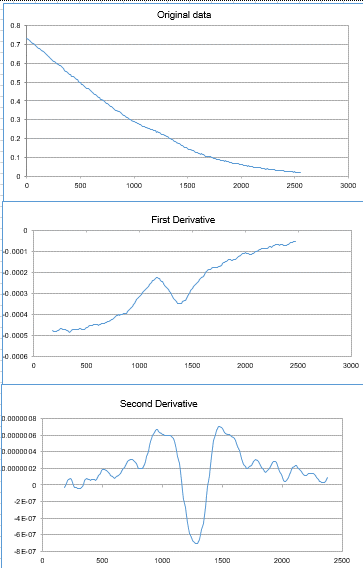
\includegraphics[width=1\textwidth]{image38.png}
    \end{minipage}\hfill
    \begin{minipage}{0.5\textwidth}
        \centering
        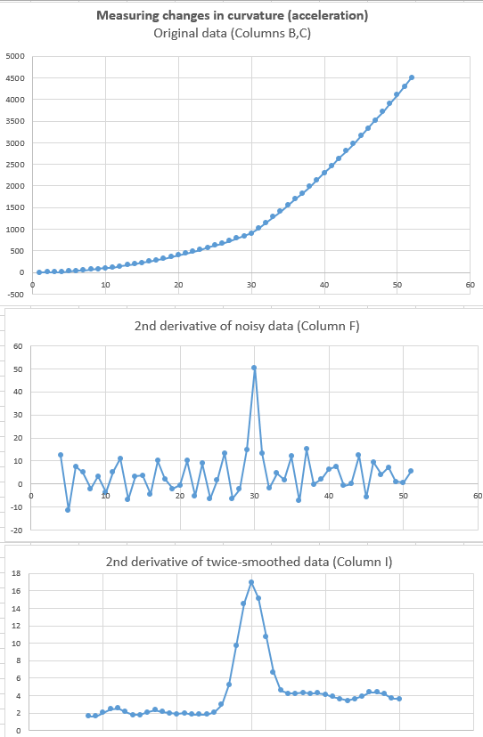
\includegraphics[width=1\textwidth]{image39.png}
    \end{minipage}
\end{figure}
Le operazioni di differenziazione come quelle descritte si possono facilmente eseguire nei fogli di calcolo come Excel o Calc di OpenOffice. Sia le derivate che le operazioni di smoothing si possono eseguire col metodo trasla-e-moltiplica descritto nel capitolo sullo \href{https://terpconnect.umd.edu/~toh/spectrum/smoothing.html}{smoothing} (pagina \pageref{ref-0045}). In linea di principio, \`{e} possibile combinare qualsiasi grado di differenziazione e di smoothing in un set di coefficienti per il trasla-e-moltiplica (\href{https://terpconnect.umd.edu/~toh/spectrum/CombinedDerivativesAndSmooths.txt}{come illustrato qui}), ma \`{e} pi\`{u} flessibile e pi\`{u} facile da regolare se si calcolano separatamente la derivata e lo smoothing in colonne successive. Ci\`{o} \`{e} illustrato da\href{https://terpconnect.umd.edu/~toh/spectrum/DerivativeSmoothing.ods}{ DerivativeSmoothing.ods} per OpenOffice Calc e da \href{https://terpconnect.umd.edu/~toh/spectrum/DerivativeSmoothing.xls}{DerivativeSmoothing.xls} per Excel, che eseguono lo smoothing dei dati e calcolano la derivata prima di Y (colonna \textbf{B}) rispetto a X (colonna \textbf{A}), poi applicano lo smoothing e la differenziazione successivamente per calcolare la derivata seconda e la terza filtrate. Gli stessi coefficienti per lo smoothing (nella riga \textbf{5}, colonne da \textbf{K} ad \textbf{AA}) vengono applicati successivamente per ciascuno stadio della differenziazione; qui si pu\`{o} inserire qualsiasi set di numeri (preferibilmente simmetrico rispetto al numero centrale nella colonna \textbf{S}). I dati si possono digitare o incollare nelle colonne \textbf{A} e \textbf{B} (X e Y), e nelle righe dalla \textbf{8} alla \textbf{26}3.

\href{https://terpconnect.umd.edu/~toh/spectrum/DerivativeSmoothingWithNoise.xlsx}{DerivativeSmoothingWithNoise.xlsx} (sopra a \href{https://terpconnect.umd.edu/~toh/spectrum/DerivativeSmoothingWithNoise.png}{sinistra}) mostra l'effetto dello smoothing sul rapporto segnale/rumore delle derivate di un flebile picco situato a x = 1200 su una linea di base inclinata. Usa gli stessi dati di \href{https://terpconnect.umd.edu/~toh/spectrum/DerivativeSmoothing.xls}{DerivativeSmoothing.xls} ma vi aggiunge del rumore bianco simulato ai dati Y. Si pu\`{o} regolare la quantit\`{a} del rumore aggiunto (cella \textbf{D5}).

Un altro esempio di applicazione della derivata \`{e} nello spreadsheet \href{https://terpconnect.umd.edu/~toh/spectrum/SecondDerivativeXY2.xlsx}{SecondDerivativeXY2.xlsx} (\href{https://terpconnect.umd.edu/~toh/spectrum/SecondDerivativeXY2.png}{a destra}), che localizza e misura l'andamento nella derivata seconda (una misura della curvatura o accelerazione) di un segnale variabile nel tempo. Questo spreadsheet mostra l'apparente aumento del rumore causato dalla differenziazione e la misura in cui il rumore pu\`{o} essere ridotto con lo smoothing (in questo caso da due passaggi di uno smoothing triangolare di 5 punti). La derivata seconda filtrata con lo smoothing mostra un ampio picco nel punto in cui cambia l'accelerazione (in x=30), ed \`{e} chiaro che la linea di base su entrambi i lati del picco \`{e} distintamente diversa, mostrando la variazione dell'accelerazione prima e dopo il picco (y=2 e 4, rispettivamente).\label{ref-0096}

\section{Differenziazione in Matlab e in \href{https://terpconnect.umd.edu/~toh/spectrum/SignalArithmetic.html\#Octave}{Octave}\label{ref-0097}\label{ref-0098}}

Le funzioni di differenziazione per differenze finite come quelle descritte si possono facilmente creare in Matlab o in \href{https://terpconnect.umd.edu/~toh/spectrum/SignalArithmetic.html\#Octave}{Octave}. Alcune semplici funzioni per le derivate di dati temporali equidistanti: \href{https://terpconnect.umd.edu/~toh/spectrum/deriv.m}{deriv}, una derivata prima col metodo della differenza centrale di 2-punti, \href{https://terpconnect.umd.edu/~toh/spectrum/deriv1.m}{deriv1}, una derivata prima senza smoothing che usa le differenze tra punti adiacenti, \href{https://terpconnect.umd.edu/~toh/spectrum/deriv2.m}{deriv2}, una derivata seconda col metodo della differenza centrale di 3-punti, una derivata terza \href{https://terpconnect.umd.edu/~toh/spectrum/deriv3.m}{deriv3} che usa la formula con 4-punti e \href{https://terpconnect.umd.edu/~toh/spectrum/deriv4.m}{deriv4}, per le derivate quarte con la formula a 5-punti. Ognuna \`{e} una semplice funzione Matlab del tipo \textbf{d=deriv(y)}; l'argomento di input \`{e} il vettore del segnale "\textbf{y}", e il segnale differenziato viene restituito nel vettore "\textbf{d}". Per i dati \textit{non} equidistanti della variabile indipendente sull'asse (x), ci sono versioni delle funzioni per la derivata prima e seconda, \href{https://terpconnect.umd.edu/~toh/spectrum/derivxy.m}{derivxy }e \href{https://terpconnect.umd.edu/~toh/spectrum/secderivxy.m}{secderivxy}, che prendono due argomenti (x,y), dove \textbf{x} e \textbf{y} sono i vettori contenenti le variabili indipendenti e dipendenti

\href{https://terpconnect.umd.edu/~toh/spectrum/SmoothDerivative.m}{SmoothDerivative.m} combina la differenziazione con lo smoothing. La sintassi \`{e} SmoothedDeriv = SmoothedDerivative(x,y,DerivativeOrder,w,type,ends) dove 'DerivativeOrder' determina l'ordine della derivata (da 0 a 5), 'w' \`{e} l'ampiezza dello smoothing, 'type' \`{e} il tipo di smoothing:

Se type=0, il segnale non subisce lo smoothing

Se type=1, \`{e} rettangolare (slittamento della media o boxcar)

Se type=2, \`{e} triangolare (2 passaggi della boxcar)

Se type=3, p-spline (3 passaggi della boxcar)

Se type=4, si applica lo smoothing di Savitzky-Golay

'ends' controlla come vengono gestite le "estremit\`{a}" del segnale (i primi w/2 punti e gli ultimi w/2 punti): Se ends=0, le estremit\`{a} vengono azzerate: Se ends=1, le estremit\`{a} subiscono uno smoothing progressivamente pi\`{u} piccolo avvicinandosi alla fine. Digitare ``help SmoothDerivative'' per degli esempi (\href{https://terpconnect.umd.edu/~toh/spectrum/SmoothDerivative.png}{grafico}).

\textbf{Rilevamento dei picchi}. Il codice pi\`{u} semplice per trovare i picchi in un insieme di dati \textit{x,y} cerca semplicemente ogni valore \textit{y} che abbia valori adiacenti \textit{y} inferiori su entrambi i lati (\href{https://terpconnect.umd.edu/~toh/spectrum/allpeaks.m}{allpeaks.m}). Un approccio alternativo consiste nell'usare la derivata prima per trovare tutti i massimi individuando i punti di passaggio per lo zero, ovvero, i punti in cui la derivata prima "d" (calcolata da \href{https://terpconnect.umd.edu/~toh/spectrum/derivxy.m}{derivxy.m}) passa da positivo a negativo. In questo esempio, la funzione ``sign'' \`{e} una funzione nativa che restituisce 1 se l'elemento \`{e} maggiore di zero, 0 se \`{e} uguale a zero e -1 se \`{e} minore di zero. La routine stampa il valore di x e di y ad ogni attraversamento dello zero:

\texttt{d=derivxy(x,y);}

\texttt{for j=1:length(x)-1}

\texttt{if sign(d(j)){\textgreater}sign(d(j+1))}

\texttt{disp([x(j) y(j)])}

\texttt{end}

\texttt{end}

Se i dati sono rumorosi, ci saranno molti attraversamenti fasulli, che per\`{o} verranno ridotti con lo smoothing dei dati. Se i dati sono scarsamente campionati, \`{e} possibile ottenere un valore pi\`{u} accurato della posizione del picco (valore sull'asse x nell'attraversamento dello zero) interpolando tra il punto precedente e quello successivo l'attraversamento dello zero, utilizzando la funzione Matlab/Octave ``interp1'' o ``spline'':

\texttt{interp1([d(j) d(j+1)],[x(j) x(j+1)],0)}

\InsImage{1.0}{DerivativeDemoMedium.png}
~\href{https://terpconnect.umd.edu/~toh/spectrum/ProcessSignal.m}{\textbf{ProcessSignal}}\textbf{\uline{.m}} \`{e} una funzione a riga di comando Matlab/Octave che esegue lo smoothing e la differenziazione di dati temporali x,y (vettori colonna e righe). Digitare "help ProcessSignal". Restituisce il segnale processato come vettore che ha la stessa forma di x, indipendentemente dalla forma di y. La sintassi \`{e} \texttt{Processed = ProcessSignal(x, y, DerivativeMode, w, type, ends, Sharpen, factor1, factor2, Symize, Symfactor, SlewRate, MedianWidth)}

\textbf{DerivativeDemo.m} \`{e} una funzione Matlab/Octave autonoma che usa \href{https://terpconnect.umd.edu/~toh/spectrum/ProcessSignal.m}{ProcessSignal.m} e \href{https://terpconnect.umd.edu/~toh/spectrum/plotit.m}{plotit.m} per mostrare un'applicazione di una differenziazione all'analisi quantitativa di un picco sepolto in un background instabile (p.es. come capita in varie forme di spettroscopia). Lo scopo \`{e} quello di ricavare la misura dell'ampiezza del picco che varia linearmente con l'effettiva ampiezza del picco ed \`{e} minimamente influenzata dal background e dal rumore. Per avviarlo, basta digitare DerivativeDemo al prompt dei comandi. Si possono modificare diverse delle variabili interne (p.es. Noise, BackgroundAmplitude) per rendere la misura pi\`{u} facile o pi\`{u} ardua. Si noti che, nonostante il fatto che l'ampiezza della derivata sembri essere numericamente inferiore al segnale originale (perch\'{e} ha unit\`{a} diverse), il rapporto segnale/rumore della derivata \`{e} migliore di quello dei segnali originali ed \`{e} molto meno influenzato dall'instabilit\`{a} del background.

\InsImageInline{0.5}{r}{AnimatedDerivative.gif.png}
~
\textbf{}\href{https://terpconnect.umd.edu/~toh/spectrum/iSignal.html}{\textbf{iSignal}}\textbf{.m} (pagina \pageref{ref-0433}), mostrato a lato) \`{e} una funzione interattiva per Matlab che esegue molte delle operazioni di signal-processing descritte, compresa la differenziazione e lo smoothing per segnali temporali, fino alla derivata 5\raisebox{4.5pt}{a}, includendo automaticamente il tipo di smoothing richiesto. Delle semplici sequenze di tasti consentono di regolare i parametri dello smoothing (il tipo, l'ampiezza e la gestione delle estremit\`{a}) mentre se ne osserva dinamicamente l'effetto sul segnale. Nella \href{https://terpconnect.umd.edu/~toh/spectrum/AnimatedDerivative.gif}{GIF animata di esempio} mostrata qui, una serie di tre picchi x=100, 250 e 400, con altezze nel rapporto 1:2:3, sono sepolte in un forte background curvo; vengono calcolate le derivate seconda e quarta con smoothing per sopprimere il background. Il codice \`{e} visualizzabile \href{https://terpconnect.umd.edu/~toh/spectrum/isignal.m}{qui} si pu\`{o} scaricare il \href{https://terpconnect.umd.edu/~toh/spectrum/iSignal7.zip}{file ZIP} con i dati dell'esempio. L'interattivit\`{a} dei tasti funziona anche se si esegue \href{https://www.mathworks.com/products/matlab-online.html}{Matlab in un browser web}, ma non su \href{https://itunes.apple.com/us/app/matlab-mobile/id370976661?mt=8}{Matlab Mobile} n\'{e} in Octave. (Nota: figure come quella precedente che mostrano la scritta ``Screencast-O-Matic'' in basso a sinistra sono grafici \textit{animati} visualizzabili in un browser web, ma non risultano animate nella maggior parte dei visualizzatori di PDF).

Come esempio di smoothing in iSignal, le istruzioni seguenti generano la derivata 4\raisebox{4.5pt}{a} di un picco Gaussiano rumoroso e lo mostrano in \textbf{iSignal}. Sar\`{a} prima necessario effettuare il download di \href{https://terpconnect.umd.edu/~toh/spectrum/isignal.m}{isignal.m}, \href{https://terpconnect.umd.edu/~toh/spectrum/gaussian.m,}{gaussian.m} e \href{https://terpconnect.umd.edu/~toh/spectrum/deriv4.m}{deriv4.m}.

\texttt{{\textgreater}{\textgreater} x=[1:.1:300]';}

\texttt{{\textgreater}{\textgreater} y=deriv4(100000.*gaussian(x,150,50)+.1*randn(size(x)));}

\texttt{{\textgreater}{\textgreater} isignal(x,y);}

Il segnale \`{e} soprattutto rumore blu (a causa della differenziazione del rumore bianco) a meno di non attenuarlo in modo considerevole. Si usano i tasti \textbf{A} e \textbf{Z} per aumentare e diminuire l'ampiezza dello smoothing e il tasto \textbf{S} per scorrere tra i diversi tipi di smoothing. Suggerimento: usare lo smoothing P-spline e continuare ad aumentare l'ampiezza dello smoothing.

Lo script ``\href{https://terpconnect.umd.edu/~toh/spectrum/iSignalDeltaTest.m}{iSignalDeltaTest}'' dimostra la risposta in frequenza delle funzioni di smoothing e di differenziazione di iSignal applicandole ad una \href{https://en.wikipedia.org/wiki/Dirac\_delta\_function}{funzione delta}. Modificando il tipo di smoothing, l'ampiezza e l'ordine di derivazione si vedr\`{a} come cambia lo spettro della potenza.

\textit{La differenziazione in tempo reale} in Matlab \`{e} trattata \href{https://terpconnect.umd.edu/~toh/spectrum/CaseStudies.html\#realtime}{a} pagina \pageref{ref-0417}\textbf{.}\label{ref-0099}

\chapter{Peak Sharpening\label{ref-0100}\label{ref-0101}}

La figura mostra uno spettro a sinistra che consiste in diverse bande scarsamente risolte (ovvero, parzialmente sovrapposte). L'ampia sovrapposizione delle bande rende impossibile la misura accurata delle loro intensit\`{a} e posizioni, anche se il rapporto segnale/rumore \`{e} ottimo. Le cose sarebbero pi\`{u} facili se le bande fossero completamente risolte, ovvero, se le bande fossero pi\`{u} strette.



\InsImage{1.0}{image41.gif.png}
\begin{center}
\textit{Un algoritmo di [peak sharpening] applicato al segnale a sinistra migliora artificialmente la risoluzione apparente dei picchi. Nel segnale risultante, a destra, si possono misurare pi\`{u} accuratamente le intensit\`{a} e le posizioni dei picchi, ma a costo di una diminuizione del rapporto segnale/rumore.}
\end{center}


\section{\textbf{Sharpening con derivata pari}\label{ref-0102}}

La tecnica utilizzata qui, chiamata \textit{[peak sharpening] o aumento della risoluzione}, usa algoritmi per migliorare artificialmente la risoluzione apparente dei picchi. Uno dei pi\`{u} semplici algoritmi di questo tipo calcola la somma ponderata del segnale originale e il negativo della sua derivata seconda:


\begin{center}
R\textsubscript{j} = Y\textsubscript{j} - k\textsubscript{2}Y\textsuperscript{''}
\end{center}


dove R\textsubscript{j} is the resolution-enhanced signal, Y is the original signal, Y'' is the second derivative of Y, and k\textsubscript{2} is a user-selected 2\textsuperscript{nd} derivative weighting factor. Viene lasciato all'utente la selezione di un fattore di ponderazione k\textsubscript{2} che offra il miglior compromesso tra la nitidezza [sharpening], la degradazione del segnale/rumore e l'appiattimento della linea di base. La scelta migliore dipende dalla larghezza, forma e dall'intervallo di digitalizzazione del segnale. Inevitabilmente, il rapporto segnale/rumore si degrada, ma questo si pu\`{o} moderare con lo \href{https://terpconnect.umd.edu/~toh/spectrum/Smoothing.html}{smoothing} (pagina \pageref{ref-0045}), ma a scapito della riduzione dello [sharpening]. Tuttavia, questa tecnica sar\`{a} \textit{utile solo se \`{e} un la sovrapposizione dei picchi \`{e} un fattore limitante piuttosto che il rapporto segnale/rumore}.

Ecco come funziona. La figura mostra, in Window 1, un picco generato al computer (con un profili Lorentziano) in rosso, sovrapposto al \textit{negativo} della sua derivata seconda in verde).


\begin{center}
\InsImage{1.0}{re1.GIF.png} 
\end{center}


La derivata seconda \`{e} amplificata (moltiplicandola per una costante modificabile) in modo che i bordi negativi della derivata seconda invertita (all'incirca da X = 0 a 100 e da X = 150 a 250) siano un'immagine speculare dei lati del picco originale in tali regioni. In questo modo, quando il picco originale viene aggiunto alla derivata seconda invertita, i due segnali \textit{quasi} si annulleranno nelle due regioni laterali ma si rafforzeranno reciprocamente in quella centrale (da X = 100 a 150). Il risultato, mostrato nella Window 2, \`{e} una sostanziale riduzione (50\% circa) della larghezza, ed un corrispondente aumento dell'altezza, del picco. Questo effetto \`{e} ancora pi\`{u} evidente con picchi di forma Lorentziana; con i picchi Gaussiani, \InsImageInline{0.5}{r}{LorentzianSharpeningExample.png}l'aumento della risoluzione \`{e} meno accentuato (\href{https://terpconnect.umd.edu/~toh/spectrum/SharpenedGaussian.png}{solo il 20 - 30\% circa}).

Le ridotte larghezze dei picchi con sharpening rendono pi\`{u} facile distinguere i picchi sovrapposti. Nell'esempio a destra, il segnale originale sintetizzato al computer (riga blu) \`{e} la somma di tre picchi Lorentziani sovrapposti a x=200, 300 e 400. I picchi sono molto larghi; le loro semi-larghezze sono 200, che \`{e} maggiore della loro separazione. Il risultato \`{e} che i picchi si sovrappongono molto nei dati originali, formando quello che \textit{sembra un unico grande picco asimmetrico} (riga blu) con un massimo a x=220. Tuttavia, il risultato dell'algoritmo di "sharpening con derivata pari" (linea rossa) mostra i picchi sottostanti \textit{nelle loro posizioni corrette}. La linea di base, tuttavia, che originariamente era zero lontano dal centro del picco, \`{e} stata spostata, come pu\`{o} vedere da x=25 a 100.

Si noti che la riga di base in entrambi i lati del picco migliorato non \`{e} molto piatto, specie per un picco Lorentziano, perch\'{e} la cancellazione tra il picco originale e la derivata seconda invertita \`{e} solo approssimata; il fattore di ponderazione k viene regolato per minimizzare minimizzare questo effetto. Lo sharpening avr\`{a} un effetto minimo, se non nessuno, sulla linea di base, perch\'{e} se la linea di base \`{e} lineare, la sua derivata sar\`{a} zero e se \`{e} gradualmente curva, la sua derivata seconda sar\`{a} molto piccola rispetto a quella del picco.

Questa tecnica \`{e} stata utilizzata in varie forme di spettroscopia e cromatografia per molti anni (riferimenti 74-76), e in qualche caso utilizzando l'elettronica analogica. Matematicamente, questa tecnica \`{e} una versione semplificata di un'espansione convergente delle \href{https://en.wikipedia.org/wiki/Taylor\_series}{serie di Taylor}, in cui vengono presi solo i termini delle derivate pari nell'espansione e per i quali i coefficienti sono di segno alterno. L'esempio precedente \`{e} la versione pi\`{u} semplice possibile che include solo i primi due termini - il picco originale e la sua derivata seconda negativa. Risultati leggermente migliori si possono ottenere aggiungendo un quarto termine derivato, con due fattori regolabili K	extsubscript{2} e K	extsubscript{4}:

Rj = Yj - K	extsubscript{2}Y'' + K	extsubscript{4}Y''''

dove Y'' e Y'''' sono le derivate 2\textsuperscript{a} e4\textsuperscript{a} di Y. Il risultato \`{e} una riduzione del 21\% in larghezza per un picco Gaussiano, come mostrato in figura (\href{https://terpconnect.umd.edu/~toh/spectrum/SharpenedGaussianDemo.m}{script Matlab/Octave}) e una riduzione del 60\% per un picco \href{https://terpconnect.umd.edu/~toh/spectrum/SharpenedLorentzianDemo.png}{Lorentziano} (\href{https://terpconnect.umd.edu/~toh/spectrum/SharpenedLorentzianDemo.m}{script}). Questo algoritmo \`{e} stato utilizzato nell'esempio precedente del picco sovrapposto. (\`{E} possibile aggiungere un \href{https://terpconnect.umd.edu/~toh/spectrum/SharpenedGaussianDemo4terms.m}{sesto termine derivativo}, ma la serie converge rapidamente e i \href{https://terpconnect.umd.edu/~toh/spectrum/SharpenedGaussianDemo4terms.png}{risultati} migliorano di poco, a costo della maggiore complessit\`{a} per avere tre fattori da regolare).

\begin{figure}
    \centering
    \begin{minipage}{0.5\textwidth}
        \centering
        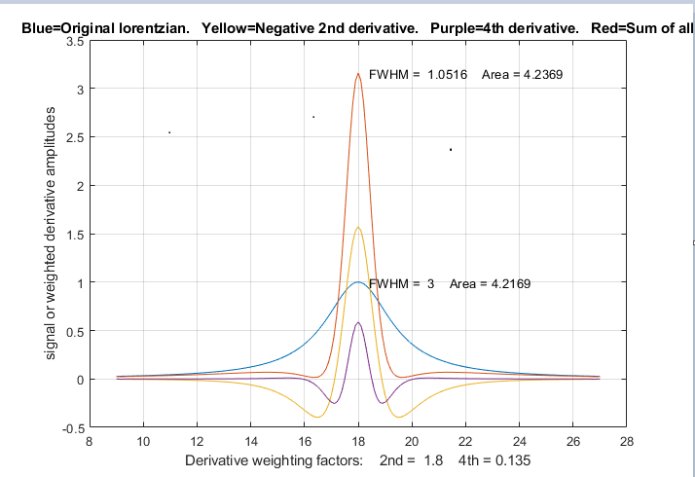
\includegraphics[width=1\textwidth]{image44.png}
    \end{minipage}\hfill
    \begin{minipage}{0.5\textwidth}
        \centering
        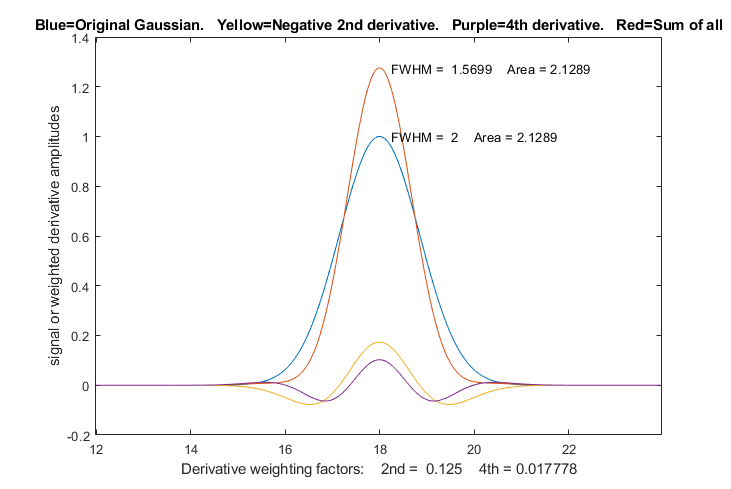
\includegraphics[width=1\textwidth]{image45.png}
    \end{minipage}
\end{figure}
Non esiste un valore ottimale universale per i fattori di ponderazione delle derivate; dipende da quello che si considera il miglior compromesso tra lo sharpening e l'appiattimento della linea di base. Tuttavia, un buon punto di partenza per un picco Gaussiano \`{e} K	extsubscript{2} = W\textsuperscript{2}/32 e K	extsubscript{4} = W\textsuperscript{4}/900, dove W \`{e} la semi-larghezza del picco in unit\`{a} x (p.es. il tempo in cromatografia). Con questi fattori, un picco Gaussiano verr\`{a} ridotto in larghezza del 21\%, la linea di base sar\`{a} ancora visivamente piatta e il picco risultante si approssimer\`{a} al modello Gaussiano con un errore di approssimazione inferiore allo 0.3\% e un R\textsuperscript{2} di 0.9999. Valori maggiori di k porteranno a picchi pi\`{u} stretti, ma la linea di base non sar\`{a} cos\`{i} piatta.  Per un picco originale Lorentziano (a destra), con K	extsubscript{2}=W\textsuperscript{3}/3 e K	extsubscript{4} = W\textsuperscript{4}/600, l'ampiezza del picco viene ridotta di un fattore 3, ma il picco risultante si approssima a un modello Gaussiano con un errore di adattamento percentuale maggiore dell'1.15\% e un R\textsuperscript{2} di 0.9966. Si noti che i fattori k per le derivate seconda e quarta variano con la larghezza W elevata alla 2\textsuperscript{a} e 4\textsuperscript{a} potenza rispettivamente, quindi possono variare su un'ampia gamma numerica per i picchi di larghezze diverse. Per questo motivo, se le larghezze dei picchi variano in modo sostanziale nel segnale, \`{e} utile utilizzare le versioni \textit{segmentate}\index{\textit{segmented}} e \textit{gradiente} di questo metodo in modo che lo sharpening si possa ottimizzare per ciascuna regione del segnale (\href{https://terpconnect.umd.edu/~toh/spectrum/ResolutionEnhancement.html\#segmented}{si veda in seguito}). ``Segmentato'' significa che ogni segmento \`{e} definito in modo indipendente; ``gradiente" indica un aumento o una diminuzione graduale tra i valori iniziali e finali specificati.

\section{\textbf{Simmetrizzazione della derivata prima con area costante (``de-tailing'')}\label{ref-0103}\label{ref-0104}\label{ref-0105}\label{ref-0106}\label{ref-0107}\label{ref-0108}\label{ref-0109}\label{ref-0110}}

Se il picco \`{e} \textit{asimmetrico} - cio\`{e}, scende pi\`{u} rapidamente su un lato rispetto all'altro - allora l'addizione ponderata (o la sottrazione) di una \textit{derivata prima}, Y', pu\`{o} essere utile, perch\'{e} la derivata prima del picco \`{e} \textit{anti-simmetrica} (positiva da un lato e negativa dall'altro). Nell'esempio grafico precedente, il picco asimmetrico (in blu) si allunga a destra e la sua derivata prima, Y', (punteggiata in giallo) ha un lobo positivo a sinistra e uno pi\`{u} largo ma pi\`{u} piccolo a destra. Quando al picco si aggiunge la derivata ponderata, il \textit{lobo positivo della derivata rinforza il bordo anteriore} e il \textit{lobo negativo sopprime il lato esteso,} con conseguente miglioramento della simmetria. (Se l'EMG fosse inclinato a \textit{sinistra}, verrebbe aggiunto il \textit{negativo} della sua derivata). Anche questa \`{e} una vecchia tecnica, essendo stata utilizzata in cromatografia almeno dal 1965 (riferimento 75, 76), dove \`{e} stata chiamata ``de-tailing''.


\begin{center}
S\textsubscript{j} = Y\textsubscript{j} + k\textsubscript{1}Y’
\end{center}


\InsImage{1.0}{image46.png}

In effetti, \`{e} possibile dimostrare che questa semplice tecnica funziona perfettamente per picchi \textit{ampliati esponenzialmente} \textit{di qualsiasi forma}, come la "\href{https://en.wikipedia.org/wiki/Exponentially\_modified\_Gaussian\_distribution}{Gaussiana espansa esponenzialmente [exponentially modified Gaussian]}" (\href{https://terpconnect.umd.edu/~toh/spectrum/expgaussian2.m}{EMG}) mostrata qui (riferimento 73).

Col giusto fattore di ponderazione della derivata prima, k\textsubscript{1}, il risultato \`{e} una Gaussiana asimmetrica con una \href{https://en.wikipedia.org/wiki/Full\_width\_at\_half\_maximum}{semi-larghezza} sostanzialmente inferiore a quella dell'originale (linea arancione); infatti, \`{e} esattamente la Gaussiana sottostante alla quale \`{e} stata applicata la convoluzione esponenziale ({\hyperref[ref-0533]{Riferimenti}} 70, 71). Il fattore di ponderazione della derivata prima k\textsubscript{1} \`{e} indipendente dall'altezza e dalla larghezza del picco ed \`{e} semplicemente uguale alla costante di tempo esponenziale \textit{tau} (1/lambda, in alcune formulazioni della EMG). Funziona perfettamente se il \textit{tau} del picco \`{e} lo stesso. In pratica, k\textsubscript{1} deve essere determinato sperimentalmente, il che \`{e} pi\`{u} facile da fare per l'ultimo picco in un gruppo di picchi (\href{https://terpconnect.umd.edu/~toh/spectrum/SymmetricalizationAnimation3peaks.png}{grafico}, \href{https://terpconnect.umd.edu/~toh/spectrum/SymmetricalizationAnimation3peaks.gif}{animazione}). In parole povere, se si ha \textsubscript{1} troppo alto, il risultato scender\`{a} al di sotto della linea di base dopo il picco. \`{E} facile determinare sperimentalmente il valore ottimale; basta aumentarlo fino a quando il segnale elaborato scende al di sotto della linea di base dopo il picco, quindi ridurlo finch\'{e} la linea di base non si appiattisce, come mostrato \href{https://terpconnect.umd.edu/~toh/spectrum/SymmetricalizationAnimation3peaks.gif}{nell'animazione GIF a questo link}. E se uno stadio della somma della derivata non funziona, si pu\`{o} provare una delle routine di doppio esponenziale descritte in seguito.

Inoltre, questo sembra essere un comportamento generale e funziona allo stesso modo per qualsiasi altra forma di picco allargata dalla convoluzione esponenziale, come una Lorentziana e funziona anche per i picchi che sono gi\`{a} stati ampliati da una precedente convoluzione esponenziale (cio\`{e} un doppio esponenziale), gestibile con due fasi successive dell'addizione delle derivate con diversi \textit{tau}.

Il picco simmetrizzato Sj risultante dalla procedura dell'addizione con la derivata prima pu\`{o} ulteriormente subire uno sharpening con le tecniche delle derivate pari descritte, supponendo che il rapporto segnale/rumore dell'originale sia abbastanza buono.

Un'utile propriet\`{a} di tutti questi algoritmi di addizione derivativa \`{e} che non cambiano l'area \textit{totale} dei picchi perch\'{e} l'area \textit{totale} della curva di \textit{ogni} derivata di un segnale con picchi che torna alla linea di base \`{e} essenzialmente \textit{zero} (l'area sotto i lobi negativi cancella l'area sotto i lobi positivi). Pertanto, queste tecniche possono risultare utili nella misura delle \href{https://terpconnect.umd.edu/~toh/spectrum/Integration.html}{aree di picchi sovrapposti} (pagina \pageref{ref-0172}). Tuttavia, un altro problema \`{e} che la linea di base su entrambi i lati del picco evidenziato con lo sharpening pu\`{o} \textit{non essere perfettamente piatto}, lasciando delle interferenze dai picchi vicini, anche se si ottiene la risoluzione della linea di base dei picchi adiacenti. Per la tecnica delle derivate pari applicata ad un picco Gaussiano, circa il 99.7\% (\href{https://terpconnect.umd.edu/~toh/spectrum/SharpenedGaussian.png}{link al grafico)} dell'area del picco \`{e} contenuta nel massimo centrale e per un picco Lorentziano, circa l'80\% dell'area del picco (\href{https://terpconnect.umd.edu/~toh/spectrum/SharpenedLorentzian.png}{link al grafico)} \`{e} contenuta nel massimo centrale.

Poich\'{e} la differenziazione e lo smoothing sono entrambe \href{https://en.wikipedia.org/wiki/Linear\_system}{tecniche lineari}, si applica il \href{https://en.wikipedia.org/wiki/Superposition\_principle}{principio di sovrapposizione} e l'ampiezza di un segnale simmetrizzato o con sharpening \`{e} direttamente proporzionale all'ampiezza del segnale originale, consentendo l'applicazione di analisi quantitative impiegando qualsiasi delle tecniche di calibrazione standard (pagina \pageref{ref-0488}). A patto di applicare le stesse tecniche di elaborazione del segnale agli standard e ai campioni, tutto funziona.

Lo sharpening dei picchi \`{e} utile nel rilevamento e nella misura automatica dei picchi (pagina \pageref{ref-0289}) per aumentare la capacit\`{a} di rilevare i deboli picchi sovrapposti che appaiono solo come sporgenze nel segnale originale. Se si sta leggendo online, click per un\href{https://terpconnect.umd.edu/~toh/spectrum/demo5.gif}{ esempio animato}. Lo sharpening dei picchi \`{e} utile anche prima di \href{https://terpconnect.umd.edu/~toh/spectrum/Integration.html}{misurare le aree} (pagina \pageref{ref-0188}) di picchi sovrapposti, perch\'{e} \`{e} pi\`{u} facile e pi\`{u} preciso misurare le aree di picchi completamente separati.

\section{\textbf{Il metodo della Legge della Potenza}\label{ref-0111}\label{ref-0112}}

\InsImageInline{0.5}{r}{PowerLawDemo.png}Un semplice metodo per lo sharpening dei picchi comporta l'innalzamento di ciascun punto a una potenza maggiore di \textbf{\textit{n}} (\href{https://terpconnect.umd.edu/~toh/spectrum/Introduction.html}{riferimenti 61}, \href{https://terpconnect.umd.edu/~toh/spectrum/Introduction.html}{63}). L'effetto di ci\`{o} \`{e} modificare le forme dei picchi, essenzialmente allungando la regione centrale pi\`{u} alta del picco ad ampiezze maggiori e ponendo pi\`{u} peso sui punti prossimi al picco, ottenendo una \textit{larghezze del picco pi\`{u} piccola.} Per i picchi Gaussiani in particolare, il risultato \`{e} un'altra Gaussiana con una larghezza ridotta della radice quadrata della potenza \textbf{\textit{n}}. La tecnica \`{e} mostrata dallo script Matlab/Octave \href{https://terpconnect.umd.edu/~toh/spectrum/PowerLawDemo.m}{PowerLawDemo.m}, mostrato in figura, che disegna Gaussiane rumorose elevate alla potenza p=1 a 7, le altezze dei picchi normalizzate a 1.0, mostrano che all'aumento della potenza, la larghezza decresce e si riduce il rumore sulla linea di base ma aumenta il massimo del picco. Poich\'{e} questo processo non sposta le posizioni dei picchi, la risoluzione del picco, la risoluzione del picco (definita come il rapporto tra la separazione del picco e la larghezza della sua base) aumenta. Per i picchi Gaussiani, l'area del picco originale si pu\`{o} calcolare dall'area sotto la curva normalizzata e trattata con lo sharpening con l'elevamento a potenza (\href{https://link.springer.com/article/10.1007\%2Fs10337-018-3607-0}{riferimento 63}).

\InsImageInline{0.5}{r}{PowerMethod.png}Nella figura, la linea blu mostra due picchi EMG ([exponentially modified Gaussian]) leggermente sovrapposti. Le altre linee sono il risultato dell'innalzamento dei dati alla potenza di \textbf{\textit{n}} = 2, 3 e 4 ciascuna normalizzata ad un'altezza di 1.00. I risultati sono molto simili a profili Gaussiani (solo perch\'{e} la maggior parte dei profili dei picchi sono localmente Gaussiane in prossimit\`{a} del massimo), e le larghezze dei picchi, misurate con la funzione \href{https://terpconnect.umd.edu/~toh/spectrum/halfwidth.m}{halfwidth.m}, sono ridotte: 19.2, 12.4, 9.9 e 8.4 unit\`{a} per le potenze da 1 a 4, rispettivamente. Questo metodo \`{e} indipendente e pu\`{o} essere utilizzato insieme al metodo derivativo discusso. Tuttavia, per un segnale di due Gaussiane sovrapposte, il risultato dell'elevamento a potenza del segnale non \`{e} lo stesso dell'addizione di due Gaussiane a potenza ridotta: semplicemente, a\textsuperscript{\textit{n}}+b\textsuperscript{\textit{n}} non \`{e} lo stesso di (a+b)\textsuperscript{\textit{n}} per \textit{n}{\textgreater}1. Ci\`{o} \`{e} dimostrato graficamente dallo script \href{https://terpconnect.umd.edu/~toh/spectrum/PowerPeaks.m}{PowerPeaks.m} (\href{https://terpconnect.umd.edu/~toh/spectrum/PowerPeaks.png}{grafico}), che approssima un modello a due Gaussiane alla somma di due Gaussiane sovrapposte elevate a potenza; all'aumentare della potenza \textit{n}, i picchi si restringono e gli avvallamenti tra di loro diventano pi\`{u} profondi, ma il segnale risultante non \`{e} pi\`{u} la somma di due Gaussiane a meno che la risoluzione sia sufficientemente alta che i due picchi non si sovrappongono in modo significativo.

Alcune delle limitazioni al metodo della legge di potenza sono:

(a) Funziona solo se i picchi di interesse fanno un massimo distinto (non \`{e} efficace per i picchi laterali che sono cos\`{i} piccoli da formare solo delle \textit{sporgenze}; ci \textit{deve} essere un avvallamento tra i picchi);

(b) La linea di base deve essere zero per ottenere i risultati migliori;

(c) Per i segnali rumorosi c'\`{e} una diminuzione del rapporto segnale-rumore perch\'{e} la larghezza minore significa che meno punti dati stanno contribuendo alla misura (lo smoothing, pagina \pageref{ref-0045}, pu\`{o} aiutare).

\textbf{Compensazione per la non linearit\`{a}}. Naturalmente, il metodo della potenza introduce una grave non linearit\`{a} nel segnale, modificando i rapporti tra le altezze dei picchi (come \`{e} evidente nella figura sopra a destra) e complicando l'ulteriore elaborazione, specie la calibrazione della misura quantitativa. Ma c'\`{e} un modo semplice per compensare questo: dopo che i dati grezzi sono stati elevati alla potenza \textit{n} e le altezze dei picchi e/o le aree sono state misurate, i picchi si possono semplicemente elevare alla potenza 1/\textit{n}, ripristinando la linearit\`{a} originale (ma, in particolare, non la pendenza) della curva di calibrazione utilizzata nella misura analitica quantitativa. (Questo funziona perch\'{e} l'area del picco \`{e} proporzionale all'altezza per la larghezza e l'altezza dei picchi elevati in potenza \`{e} proporzionale alla potenza ennesima dell'altezza originale, ma l'ampiezza del picco non \`{e} una funzione dell'altezza del picco alla costante \textit{n}, quindi l'area dei picchi trasformati resta proporzionale alla potenza ennesima dell'altezza originaria). La tecnica \`{e} dimostrata quantitativamente per due picchi sovrapposti variabili dallo script Matlab/Octave \href{https://terpconnect.umd.edu/~toh/spectrum/PowerLawCalibrationDemo.m}{PowerLawCalibration-Demo.m} (\href{https://terpconnect.umd.edu/~toh/spectrum/PowerLawCalibrationDemo.png}{grafico}), che prende la potenza \textit{n}\textsuperscript{esima} del segnale del picco sovrapposto, misura le aree dei trasformati e poi calcola la potenza 1/\textit{n} delle aree misurate, costruendo e utilizzando una curva di calibrazione per convertire le aree in concentrazioni. Le aree dei picchi vengono misurate mediante tagli verticali, utilizzando il punto a met\`{a} percorso per contrassegnare il confine tra i picchi. Lo script simula un segnale misto con concentrazioni indicabili nelle righe 15 e 16. \`{E} possibile modificare la potenza e qualsiasi parametro nelle righe 14-22. I risultati mostrano che il metodo della potenza migliora l'accuratezza delle misure fintanto che la risoluzione 4-sigma (il rapporto tra la separazione del picco e 4 volte la sigma delle Gaussiane) a all'incirca superiore a 0.4. \`{E} pi\`{u} accurato quando i picchi sono approssimativamente uguali in larghezza e quando il rapporto tra le due concentrazioni non \`{e} molto diverso dal rapporto negli standard da cui viene costruita la curva di calibrazione. Si noti che, anche quando il rumore casuale (nella riga 22) \`{e} zero, i risultati non sono perfetti a causa dell'effetto della sovrapposizione dei picchi sulla misura dell'area, che varia a seconda del rapporto tra le due componenti nella miscela.

La funzione autonoma \href{https://terpconnect.umd.edu/~toh/spectrum/PowerMethodDemo.m}{PowerMethodDemo.m} mostra il metodo dell'elevamento a potenza per misurare l'area del piccolo picco sporgente che \`{e} parzialmente sovrapposto da un picco che interferisce molto pi\`{u} forte (\href{https://terpconnect.umd.edu/~toh/spectrum/PowerMethod2.png}{grafico}). Mostra l'effetto del rumore casuale, dello smoothing e di qualsiasi background incorretto sotto i picchi.

\textbf{Combinare i metodi di sharpening}. Il metodo dell'elevamento a potenza \`{e} indipendente da, e pu\`{o} essere utilizzato con, i metodi derivativi discussi. Tuttavia, poich\'{e} il metodo della potenze non \`{e} lineare, l'ordine \textit{con cui le operazioni sono} eseguite \`{e} importante. Il \textit{primo} passaggio dovrebbe essere la simmetrizzazione con la derivata prima se il segnale \`{e} espanso esponenzialmente, il \textit{secondo} passo dovrebbe essere lo sharpening derivativo e il metodo dell'elevamento a potenza dovrebbe essere l'\textit{ultimo}. Il motivo di questo ordine \`{e} che il metodo della potenza dipende da, ma non pu\`{o} creare, una valle tra i picchi molto sovrapposti, mentre i metodi delle derivate \hspace{0pt}possono essere in grado di creare una valle tra i picchi se la sovrapposizione non \`{e} eccessiva. Inoltre, quando utilizzato per ultimo, il metodo della potenza riduce la severit\`{a} delle oscillazioni della linea di base che sono un residuo dello sharpening con le derivate pari (particolarmente evidente nel picco Lorentziano). Gli script Matlab/Octave\href{https://terpconnect.umd.edu/~toh/spectrum/SharpenedGaussianDemo2.m}{SharpenedGaussianDemo2.m} (\href{https://terpconnect.umd.edu/~toh/spectrum/SharpenedGaussianDemo2.png}{Grafico}) e \href{https://terpconnect.umd.edu/~toh/spectrum/SharpenedLorentzianDemo2.m}{SharpenedLorentzianDemo2.m} (\href{https://terpconnect.umd.edu/~toh/spectrum/SharpenedLorentzianDemo2.png}{Grafico}) rendono questo punto per picchi Gaussiani e Lorentziani rispettivamente, confrontando il risultato del solo sharpening con le derivate pari con quello dello sharpening con le derivate pari seguito dal metodo dell'elevamento a potenza (ed eseguendo il metodo della potenza in due modi, prendendo il quadrato del picco con sharpening o moltiplicandolo per il picco originale). Sia per le forme Gaussiane che per le Lorentziane di partenza, i risultati finali dello sharpening si adattano ai modelli Gaussiani per mostrare i cambiamenti dei parametri dei picchi. Il risultato \`{e} che la combinazione di metodi produce (a) il picco finale pi\`{u} stretto e (b) il pi\`{u} vicino al profilo finale Gaussiano. Naturalmente, restano i problemi con la linearit\`{a} del metodo della potenza, ma si possono compensare come in precedenza.

\textbf{Deconvoluzione}. Un'altra tecnica di elaborazione del segnale che pu\`{o} aumentare la risoluzione dei picchi sovrapposti \`{e} la \textit{deconvoluzione} (pagina \pageref{ref-0147}). \`{E} applicabile quando il profilo originale dei picchi \`{e} stato espanso e/o reso asimmetrico con qualche processo o funzione di espansione. Se il processo di espansione \`{e} descrivibile matematicamente o misurato a parte, allora la deconvoluzione dai picchi espansi osservati \`{e} in linea di principio in grado di estrarre il profilo del picco sottostante.

\href{https://terpconnect.umd.edu/~toh/spectrum/SPECTRUM.html}{SPECTRUM,} pagina \pageref{ref-0481}, l'applicazione freeware di signal-processing per Mac OS8 e precedenti, include questo algoritmo di miglioramento della risoluzione, col fattore di ponderazione e l'ampiezza dello smoothing derivativo regolabili.

\section{\textbf{Peak Sharpening per fogli di calcolo Excel e Calc}\label{ref-0113}}

Il metodo di sharpening con derivate pari con due termini derivativi (2\textsuperscript{a} e 4\textsuperscript{a}) \`{e} disponibile per Excel e Calc sotto forma di un template vuoto (\href{https://terpconnect.umd.edu/~toh/spectrum/PeakSharpeningDeriv.xlsx}{PeakSharpeningDeriv.xlsx} e \href{https://terpconnect.umd.edu/~toh/spectrum/PeakSharpeningDeriv.ods}{.ods}) o con la presenza di dati di esempio (\href{https://terpconnect.umd.edu/~toh/spectrum/PeakSharpeningDerivWithData.xlsx}{PeakSharpeningDerivWithData.xlsx} e \href{https://terpconnect.umd.edu/~toh/spectrum/PeakSharpeningDerivWithData.ods}{.ods}). \`{E} possibile inserire i valori dei fattori di ponderazione delle derivate K1 e K2 direttamente nelle celle \textbf{J3} e \textbf{J4}, oppure si possono inserire l'ampiezza stimata del picco (FWHM in numero di punti) nella cella \textbf{H4} e lo spreadsheet calcoler\`{a} K1 e K2. Esiste anche una versione dimostrativa con picchi simulati regolabili con cui sperimentare(\href{https://terpconnect.umd.edu/~toh/spectrum/PeakSharpeningDemo.xlsx}{PeakSharpeningDemo.xlsx} e \href{https://terpconnect.umd.edu/~toh/spectrum/PeakSharpeningDemo.ods}{PeakSharpeningDemo.ods}).

\InsImageInline{0.5}{r}{ClickButtons.png}
Esistono anche \href{https://terpconnect.umd.edu/~toh/spectrum/PeakSharpeningDemo.xlsm}{versioni che hanno pulsanti} cliccabili (i dettagli a lato) per una comoda regolazione interattiva dei fattori K1 e K2 dell'1\% o del 10\% per ogni click. Si possono inserire direttamente le prime stime di K1 e K2 nelle celle J4 e J5 e poi usare i pulsanti per affinare i valori. Se il segnale \`{e} rumoroso, regolare il livellamento utilizzando i 17 coefficienti nella riga 5 delle colonne da \textbf{K} ad \textbf{AA}, proprio come con i \href{https://terpconnect.umd.edu/~toh/spectrum/Differentiation.html\#Spreadsheets}{fogli di calcolo per lo smoothing} (pagina \pageref{ref-0068}). (Nota: Sfortunatamente, questi pulsanti ActiveX non funzionano nella versione iPad di Excel).

Esiste anche un versione ``segmentata'' del template in cui \`{e} possibile specificare le costanti per lo sharpening per ognuno dei 20 segmenti del segnale (\href{https://terpconnect.umd.edu/~toh/spectrum/SegmentedPeakSharpeningDeriv.xlsx}{SegmentedPeakSharpeningDeriv.xlsx}). Per quelle applicazioni in cui le larghezze dei picchi aumentano (o diminuiscono) gradualmente nel tempo, c'\`{e} anche un template per lo sharpening del picco con \textit{gradiente} in cui basta impostare la larghezza del picco iniziale e quella del picco finale e il foglio di calcolo applicher\`{a} il fattori di sharpening richiesti K1 e K2. (\href{https://terpconnect.umd.edu/~toh/spectrum/GradientPeakSharpeningDeriv.xlsx}{GradientPeakSharpeningDeriv.xlsx}) e un esempio con dati gi\`{a} inseriti \href{https://terpconnect.umd.edu/~toh/spectrum/GradientPeakSharpeningDerivExample.xlsx}{GradientPeakSharpeningDerivExample.xlsx});

Il template \href{https://terpconnect.umd.edu/~toh/spectrum/PeakSymmetricalizationTemplate.xlsm}{PeakSymmetricalizationTemplate.xlsm} (schermata di seguito) esegue la simmetrizzazione delle Gaussiane modificate esponenzialmente [exponentially modified Gaussians] (EMG) mediante l'aggiunta ponderata della derivata prima. \href{https://terpconnect.umd.edu/~toh/spectrum/PeakSymmetricalizationTemplate.xlsm}{PeakSymmetricalizationExample.xlsm} \`{e} un'applicazione con dei dati di esempio gi\`{a} inseriti. Mostrata in seguito.

C'\`{e} anche una versione demo che consente di determinare l'accuratezza della tecnica sintetizzando picchi sovrapposti con risoluzione, asimmetria, altezza relativa del picco, rumore e linea di base specificati: \href{https://terpconnect.umd.edu/~toh/spectrum/PeakSharpeningAreaMeasurementEMGDemo2.xlsm}{PeakSharpeningAreaMeasurementEMGDemo2.xlsm} (\href{https://terpconnect.umd.edu/~toh/spectrum/PeakSharpeningAreaMeasurementDemoEMG3.png}{grafico}). Questi fogli di calcolo consentono anche un ulteriore sharpening con la derivata seconda del picco simmetrico risultante.

\href{https://terpconnect.umd.edu/~toh/spectrum/PeakDoubleSymmetrizationExample.xlsm}{PeakDoubleSymmetrizationExample.xlsm} esegue la simmetrizzazione di un picco doppiamente allargato esponenzialmente. Dispone di pulsanti per regolare interattivamente i due pesi della derivata prima. Due varianti (\href{https://terpconnect.umd.edu/~toh/spectrum/PeakDoubleSymmetrizationExample1.xlsm}{1}, \href{https://terpconnect.umd.edu/~toh/spectrum/PeakDoubleSymmetrizationExample2.xlsm}{2}) includono i dati per due picchi sovrapposti, per i quali le aree vengono misurate con un taglio perpendicolare.

\href{https://terpconnect.umd.edu/~toh/spectrum/EffectOfNoiseAndBaselineNormalVsPower.xlsx}{EffectOfNoiseAndBaselineNormalVsPower.xlsx} mostra l'effetto del metodo dell'elevamento a potenza sulle misure delle aree di picchi Gaussiani Gaussiani allargati esponenzialmente, inclusi i diversi effetti che hanno il rumore casuale e una linea di base non nulla sullo sharpening.

\InsImageInline{0.5}{r}{image50.png}\textit{Viene mostrato il} \textit{template} \textbf{\textit{\textnormal{dello spreadsheet ``}}}\href{https://terpconnect.umd.edu/~toh/spectrum/PeakSymmetricalizationTemplate.xlsm}{\textit{PeakSymmetricalizationTemplate.xlsm}}\textit{'' viene mostrato misurando le aree della prima e della seconda coppia di picchi asimmetrici sovrapposti dopo aver applicato la simmetrizzazione con la derivata prima.}\label{ref-0114}

\section{\textbf{Sharpening dei picchi per Matlab e} \href{https://terpconnect.umd.edu/~toh/spectrum/SignalArithmetic.html\#Octave}{\textbf{Octave}}\label{ref-0115}}

La funzione utente per Matlab/Octave \href{https://terpconnect.umd.edu/~toh/spectrum/sharpen.m}{sharpen} ha la forma \texttt{SharpenedSignal = sharpen (signal,k1,k2, SmoothWidth)}, dove "signal" \`{e} il vettore del segnale originale, gli argomenti K	extsubscript{2} e K	extsubscript{4} sono i fattori di ponderazione della derivata 2\textsuperscript{a} e 4\textsuperscript{a} e SmoothWidth \`{e} la larghezza dello smoothing. Il segnale migliorato in risoluzione viene restituito nel vettore "SharpenedSignal". Se si sta leggendo online, si pu\`{o} cliccare sul link sopra per ispezionare il codice o fare click-destro del mouse per scaricarlo per utilizzarlo all'interno di Matlab o di Octave. I valori \textbf{k} determinano il compromesso tra la nitidezza [sharpness] del picco e l'appiattimento della linea di base; i valori variano in base alla forma e alla larghezza del picco e devono essere regolati in base alle proprie necessit\`{a}. Per i picchi con profilo Gaussiano, un valore ragionevole per k\textsubscript{2} \`{e} PeakWidth\textsuperscript{2}/32 e per k\textsubscript{4} \`{e} PeakWidth\textsuperscript{4}/900 (o PeakWidth\textsuperscript{2}/8 e PeakWidth\textsuperscript{4}/700 per picchi Lorentziani), dove PeakWidth \`{e} la larghezza totale a met\`{a} massimo dei picchi in unit\`{a} x. Poich\'{e} i metodi di sharpening sono tipicamente sensibili al rumore casuale nel segnale, \`{e} solitamente necessario applicare un'operazione di smoothing: la funzione Matlab/Octave \href{https://terpconnect.umd.edu/~toh/spectrum/ProcessSignal.m}{ProcessSignal.m} consente di applicare sia lo sharpening che lo smoothing in un'unica funzione.

Ecco un semplice esempio Matlab/Octave che crea un segnale composto da quattro picchi Gaussiani parzialmente sovrapposti di uguale altezza e larghezza, applica sia il metodo di sharpening derivativo che quello dell'elevamento a potenza e confronta un grafico (mostrato di seguito) del segnale originale (in blu) con la versione a risoluzione migliorata (in rosso).

\texttt{x=0:.01:18;}

\texttt{y=exp(-(x-4).\textasciicircum{}2)+exp(-(x-9).\textasciicircum{}2)+exp(-(x-12).\textasciicircum{}2)+exp(-(x-13.7).\textasciicircum{}2);}

\texttt{y=y+.001.*randn(size(x));}

\texttt{k1=1212;k2=1147420;}

\texttt{SharpenedSignal=ProcessSignal(x,y,0,35,3,0,1,k1,k2,0,0,0,0);}

\texttt{figure(1)}

\texttt{plot(x,y,x,SharpenedSignal,'r')}

\texttt{title('Peak sharpening (red) by the derivative method')}

\texttt{figure(2)}

\texttt{plot(x,y,x,y.\textasciicircum{}6,'r')}

\texttt{title('Peak sharpening (red) by the power method')}


\begin{center}
\InsImageInline{0.5}{r}{DerivSharp4peaks.png}
\end{center}



\begin{center}
\textit{Quattro picchi Gaussian sovrapposti di uguale altezza e larghezza.}
\end{center}



\begin{center}
\textit{In blu: L'originale. In Rosso: Dopo lo sharpening col metodo delle derivate pari.}
\end{center}


\InsImageInline{0.5}{r}{SharpenedOverlapDemo2.png}\href{https://terpconnect.umd.edu/~toh/spectrum/SharpenedOverlapDemo.m}{SharpenedOverlapDemo.m} \`{e} uno script che \textit{automaticamente determina il grado ottimale di sharpening con le derivate pari} che minimizza gli errori nella misura delle aree dei picchi di due Gaussiane sovrapposte col metodo del taglio perpendicolare utilizzando la funzione autopeaks.m. Lo fa applicando diversi gradi di sharpening e disegnando gli errori delle aree (differenza percentuale tra gli errori veri e quelli misurati) rispetto al fattore di sharpening, come mostrato in figura. Mostra anche l'altezza della valle tra i picchi (linea gialla). Questo dimostra che:

(1) il fattore ottimale di sharpening dipende dalla larghezza e dalla separazione dei due picchi e dal rapporto delle loro altezze;

(2) il grado di sharpening non \`{e} eccessivamente critico, mostrando spesso un'ampia regione ottimale;

(3) l'ottimo per i due picchi non \`{e} necessariamente lo stesso; e

(4) l'ottimo per la misura delle aree non si ha necessariamente nel punto in cui si azzera l'avvallamento.

(Per eseguire questo script si devono avere gaussian.m, derivxy.m, autopeaks.m, val2ind.m e halfwidth.m nel path. Il download si effettua da \url{https://terpconnect.umd.edu/~toh/spectrum/}).

\InsImageInline{0.5}{r}{PowerLaw4peaks.png}\textbf{Il metodo dell'elevamento a potenza} \`{e} efficace se c'\`{e} un avvallamento tra i picchi sovrapposti, ma questo introduce una non-linearit\`{a} che dev'essere corretta in seguito, mentre il metodo delle derivate preserva le aree originali dei picchi e il rapporto tra le altezze dei picchi. \href{https://terpconnect.umd.edu/~toh/spectrum/PowerLawCalibrationDemo.m}{PowerLawCalibrationDemo} mostra la linearizzazione delle curve di calibrazione trasformate in potenza per due picchi sovrapposti prendendo la potenza ennesima dei dati, localizzando l'avvallamento tra di essi, misurando le aree col metodo del taglio perpendicolare (pagina \pageref{ref-0184}), e quindi prendendo la potenza 1/n delle aree misurate (\href{https://terpconnect.umd.edu/~toh/spectrum/PowerTransformCalibrationCurve.png}{grafico}).

\InsImageInline{0.5}{r}{SymmetizedOverlapDemo.png}\textbf{La simmetrizzazione ad area costante (de-tailing) di picchi asimmetrici} mediante l'aggiunta ponderata della derivata prima viene eseguita dalla funzione ySym =\href{https://terpconnect.umd.edu/~toh/spectrum/symmetrize.m}{ symmetrize}(t,y,factor,smoothwidth,type,ends); "t" e "y" sono i vettori della variabile indipendente e di quella dipendente, "factor" \`{e} il fattore di ponderazione della derivata prima, "smoothwidth", "type" e "ends" sono i parametri \href{https://terpconnect.umd.edu/~toh/spectrum/SegmentedSmooth.m}{SegmentedSmooth} per lo smoothing derivativo interno. Per eseguire una simmetrizzazione segmentata, "factor" e "smoothwidth" possono essere dei vettori. Nella versione 2, symmetrize.m esegue solo lo smoothing della derivata, non dell'intero segnale. \href{https://terpconnect.umd.edu/~toh/spectrum/SymmetrizeDemo.m}{SymmetrizeDemo.m} esegue tutti e cinque gli esempi nel file di help symmetrize.m, ciascuno in una finestra separata. Se il tau \textit{non} \`{e} noto, lo si pu\`{o} determinate per un singolo picco isolato utilizzando AutoSymmetrize(t, y, SmoothWidth, plots), che cerca il valore di tau che produce il picco pi\`{u} simmetrico, confrontando la pendenza delle tangenti sui lati di entrata e di uscita. Nell'esempio a lato, il picco originale (linea blu) \`{e} una Gaussiana modificata esponenzialmente calcolata matematicamente con un valore di tau di 100 e la linea rossa \`{e} l'output generato da AutoSymmetrize, che stima il tau con un'accuratezza dell'1\%. Digitare ``help AutoSymmetrize''. Le aree dei due sono uguali entro lo 0.01\%. \href{https://terpconnect.umd.edu/~toh/spectrum/SymmetizedOverlapDemo.m}{SymmetizedOverlapDemo.m} mostra l'ottimizzazione della simmetrizzazione con la derivata prima per la misura delle aree di due Gaussiane sovrapposte allargate esponenzialmente.

\InsImageInline{0.5}{r}{SegmentedSharpenDemo.png}\textbf{Sharpening segmentato dei picchi con derivate pari}. Se la larghezza dei picchi o la varianza del rumore varia sostanzialmente lungo il segnale, si pu\`{o} usare la versione \textit{segmentata}\index{\textcolor{color-3}{segmented}} \href{https://terpconnect.umd.edu/~toh/spectrum/SegmentedSharpen.m}{SegmentedSharpen.m}, per cui gli argomenti factor1, factor2 e SmoothWidth sono \textit{vettori}. Lo script \href{https://terpconnect.umd.edu/~toh/spectrum/DemoSegmentedSharpen.m}{DemoSegmentedSharpen.m}, mostrato a lato, usa questa funzione per eseguire lo sharpening di quattro picchi Gaussiani con larghezze dei picchi gradualmente crescenti da sinistra a destra con un crescente grado di sharpening, mostrando che la larghezza del picco viene \href{https://terpconnect.umd.edu/~toh/spectrum/SegmentedSharpenDemo.txt}{ridotta dal 20\% al 22\%} rispetto all'originale.

\href{https://terpconnect.umd.edu/~toh/spectrum/DemoSegmentedSharpen2.m}{DemoSegmentedSharpen2.m} mostra quattro picchi con la \textit{stessa} larghezza cui si applica un grado crescente di sharpening.

\textbf{\InsImageInline{0.5}{r}{image56.png}La simmetrizzazione esponenziale doppia} in Matlab/Octave viene eseguita dalla funzione \href{https://terpconnect.umd.edu/~toh/spectrum/DEMSymm.m}{DEMSymm.m} che applica due successive addizioni ponderate della derivata prima, con fattori di ponderazione idealmente uguali ai due tau. L'obiettivo \`{e} rendere i picchi pi\`{u} simmetrici e pi\`{u} stretti preservandone l'area. \uppercase{Una tecnica} di [bracketing] a tre livelli pi\`{u}-e-meno aiuta a determinare i valori migliori per i due fattori di ponderazione. La tecnica viene mostrata dallo script \href{https://terpconnect.umd.edu/~toh/spectrum/DemoDEMSymm.m}{DemoDEMSymm.m} e sono due varianti (\href{https://terpconnect.umd.edu/~toh/spectrum/DemoDEMSymm2.m}{1}, \href{https://terpconnect.umd.edu/~toh/spectrum/DemoSymm3.m}{2}), che creano due picchi sovrapposti doppiamente esponenziali dagli originali Gaussiani, poi chiama la funzione DEMSymm.m per eseguire la simmetrizzazione. Nell'esempio a lato, in mezzo alle tre linee di [bracketing] c'\`{e} il valore ottimale.\label{ref-0116}

In sintesi, se si tenta di simmetrizzare un picco asimmetrico mediante l'aggiunta ponderata della derivata prima e il risultato \`{e} ancora asimmetrico, \`{e} possibile che l'asimmetria residua sia dovuta a un altro stadio di ampliamento esponenziale con un diverso \textit{tau}, quindi in tal caso, l'applicazione di DEMSymm.m produrr\`{a} probabilmente un risultato finale pi\`{u} simmetrico.

\href{https://terpconnect.umd.edu/~toh/spectrum/ProcessSignal.m}{ProcessSignal}, una funzione Matlab/Octave a riga di comando che esegue smoothing, differenziazione e sharpening del picco su una serie temporale x,y (vettori colonne o righe). Digitare "help ProcessSignal". Restituisce il segnale processato come vettore che ha lo stesso profilo di x, indipendentemente da quello di y.

\texttt{Processed=Processed=ProcessSignal(x,y,DerivativeMode, w, type, ends, Sharpen, factor1, factor2, Symize, Symfactor, SlewRate, MedianWidth)}

\href{https://terpconnect.umd.edu/~toh/spectrum/iSignal.html}{\textbf{iSignal}} (Versione 8.3, pagina \pageref{ref-0433}) \`{e} una funzione interattiva Matlab multi-uso che include lo sharpening per segnali temporali, utilizzando \textit{sia} il metodo delle derivate pari (funzione \textit{sharpen} ) che quello della simmetrizzazione con la derivata prima, consente di regolare da tastiera i fattori di ponderazione delle derivate e dello smoothing in modo continuo osservando dinamicamente l'effetto sul segnale. Il tasto \textbf{E} attiva e disattiva la funzione di sharpening dei picchi. Il codice \`{e} visualizzabile \href{https://terpconnect.umd.edu/~toh/spectrum/isignal.m}{qui} o si pu\`{o} scaricare il \href{https://terpconnect.umd.edu/~toh/spectrum/iSignal7.zip}{file ZIP} con i dati dell'esempio per il test. \textit{iSignal} calcola le impostazioni di sharpening e smoothing per picchi Gaussiani e Lorentziani utilizzando rispettivamente i tasti \textbf{Y} e \textbf{U}, e usando l'espressione precedente. Basta isolare un solo picco tipico nella finestra superiore con i tasti pan e zoom, poi premere \textbf{P} nella modalit\`{a} di misura del picco e poi premere \textbf{Y} per picchi Gaussiani o \textbf{U} per quelli Lorentziani. \`{E} possibile ottimizzare lo sharpening con i tasti \textbf{F/V} e \textbf{G/B} e lo smoothing con i tasti \textbf{A/Z}. (Se il segnale ha picchi di larghezze molto diverse, un unico settaggio non sar\`{a} ottimale per tutti i picchi. In questi casi si pu\`{o} usare la funzione di\index{\textcolor{color-3}{segmented}} sharpening segmentato, \href{https://terpconnect.umd.edu/~toh/spectrum/SegmentedSharpen.m}{SegmentedSharpen.m}).


\begin{center}
\InsImageInline{0.5}{r}{ps1.png}\InsImageInline{0.5}{r}{ps2.png} \textit{Prima dello Sharpening in iSignal Dopo lo sharpening in iSignal}
\end{center}


\InsImageInline{0.5}{r}{image59.png}In \textit{iSignal}, e in \textit{iPeak}, il tasto \textbf{Shift-Y} attiva la tecnica di simmetrizzazione della derivata prima (a sinistra) ed usa i tasti \textbf{1}, \textbf{Shift-1}, \textbf{2}, e \textbf{Shift-2} per regolare il fattore di ponderazione del 10\% o dell'1\% ad ogni pressione del tasto. Aumentare il fattore fino a quando la linea di base dopo il picco diventa negativa, quindi si aumenta leggermente in modo che sia \textit{il pi\`{u} basso possibile ma non negativo}.

\textit{iSignal} pu\`{o} anche utilizzare il metodo di trasformazione con la potenza (si preme il tasto \textbf{\textasciicircum{}}, si inserisce la potenza, \textit{n} (qualsiasi numero positivo maggiore di 1.00) e si preme \textbf{Enter}. Per invertirlo, basta elevare alla potenza 1/\textit{n}. \href{https://terpconnect.umd.edu/~toh/spectrum/PeakFindingandMeasurement.htm\#ipeak}{\textit{iPeak}}, (pagina \pageref{ref-0320}), \`{e} un programma Matlab interattivo per il rilevamento e la misura dei picchi, ha una modalit\`{a} di sharpening basata sulla tecnica delle derivate pari, nonch\'{e} quella di simmetrizzazione con la derivata prima utilizzando gli stessi tasti di \textit{iSignal}. Vedere \href{https://terpconnect.umd.edu/~toh/spectrum/PeakFindingandMeasurement.htm\#demos}{ipeakdemo5} a pagina \pageref{ref-0324}. L'animazione GIF \url{https://terpconnect.umd.edu/~toh/spectrum/iPeakShiftYDeTail.gif} lo mostra in azione.

\textit{Lo sharpening in tempo reale} in Matlab \`{e} trattato a pagina \pageref{ref-0418}.\label{ref-0117}\label{ref-0118}\label{ref-0119}\label{ref-0120}

\chapter{Analisi delle armoniche e la Trasformata di Fourier.\label{ref-0121}\label{ref-0122}}

Alcuni segnali mostrano componenti periodiche che si ripetono a intervalli fissi per tutto il segnale, come un'onda sinusoidale. \`{E} spesso utile descrivere esattamente l'ampiezza e la frequenza di tali componenti periodiche. Infatti, \`{e} possibile analizzare \textit{qualsiasi} insieme di dati arbitrari nelle sue componenti periodiche, sia che i dati appaiano periodici o meno. \href{http://resonanceswavesandfields.blogspot.com/2009/01/spectrum-of-waveform-fourier-analysis.html}{L'analisi armonica} \`{e} convenzionalmente basata sulla \href{http://en.wikipedia.org/wiki/Discrete\_Fourier\_transform}{\textit{trasformata di Fourier}}, che \`{e} un modo per esprimere un segnale come somma di \href{http://en.wikipedia.org/wiki/Sine\_wave}{seni e coseni}. Si pu\`{o} dimostrare che qualsiasi segnale arbitrario campionato discretamente pu\`{o} essere descritto completamente dalla somma di un numero finito di componenti seno e coseno le cui frequenze sono 0, 1, 2, 3 ... n/2 volte la frequenza f=1/n${\Updelta}$x, dove ${\Updelta}$x \`{e} l'intervallo tra i valori adiacenti di x e n \`{e} il numero totale di punti. La trasformata di Fourier \`{e} semplicemente l'insieme delle ampiezze di quelle componenti seno e coseno (o, che \`{e} equivalente matematicamente\href{ftp://www.myphysicslab.com/trig\_identity1.html}{, la frequenza e la fase delle componenti seno}). Quei coefficienti si potrebbero calcolare semplicemente ma laboriosamente moltiplicando il segnale punto per punto con ciascuna di quelle componenti seno e coseno e sommando i prodotti. La famosa ``\href{https://pdfs.semanticscholar.org/1790/fe007bc1ab161a1ea814748b42e3acbdc958.pdf}{Fast Fourier Transform}'' (FFT) risale al 1965 ed \`{e} un algoritmo pi\`{u} veloce ed efficiente che utilizza la simmetria delle funzioni seno e coseno e altre scorciatoie matematiche per ottenere lo stesso risultato \href{https://terpconnect.umd.edu/~toh/spectrum/HarmonicAnalysis.html\#sft}{\textit{molto} pi\`{u} rapidamente}. La trasformata \textit{inversa} di Fourier (IFT) \`{e} un algoritmo simile che converte una trasformata di Fourier nel segnale originale. Per comodit\`{a} matematica, le trasformate di Fourier sono solitamente espresse in termini di ``\href{https://en.wikipedia.org/wiki/Complex\_number}{numeri complessi}'', perch\'{e} le parti ``reali'' e ``immaginarie'' consentono di combinare le informazioni di seno e coseno (o ampiezza e fase) per ciascuna frequenza in un unico numero complesso, utilizzando l'identit\`{a} $\exp \left(i2\pi ft\right)=\cos \left(2\pi ft\right)+isin\left(2\pi ft\right).$ Anche per i dati che non sono complessi, usare la ``exp'' anzich\'{e} ``sin+cos'' \`{e} pi\`{u} compatto ed elegante, e molti linguaggi per computer possono gestire automaticamente aritmetiche complesse quando le quantit\`{a} sono complesse. Ma questa terminologia pu\`{o} essere fuorviante: le parti seno e coseno sono \textit{ugualmente importanti}; solo perch\'{e} le due parti sono chiamate "reale" e "immaginaria" in matematica non implica che la prima sia meno significativa della seconda.

Il concetto di trasformata di Fourier \`{e} coinvolto in due moderni metodi strumentali molto importanti in chimica. Nella \href{http://en.wikipedia.org/wiki/Fourier\_transform\_spectroscopy}{Spettroscopia infrarossa in trasformata di Fourier (FTIR)}, la trasformata di Fourier dello spettro viene misurata direttamente dallo strumento, come l'interferogramma formato tracciando il segnale del rivelatore rispetto allo spostamento dello specchio in un interferometro di Michaelson a scansione. Nella \href{http://en.wikipedia.org/wiki/NMR\#Fourier\_spectroscopy}{spettroscopia di risonanza magnetica nucleare in trasformata di Fourier (FTNMR)}, l'eccitazione del campione da parte di un intenso e breve impulso di energia a radiofrequenza produce un segnale di decadimento di induzione libera che \`{e} la trasformata di Fourier dello spettro della risonanza. In entrambi i casi, viene usato un computer per acquisire lo spettro mediante trasformata inversa di Fourier del segnale misurato (interferogramma o decadimento di induzione libera).

Lo \href{http://en.wikipedia.org/wiki/Frequency\_spectrum}{\textit{spettro della potenza}} o \textit{spettro delle frequenze} \`{e} un semplice modo per mostrare l'ampiezza totale in ciascuna di queste frequenze. Viene calcolato come la radice quadrata della somma dei quadrati dei coefficienti delle componenti seno e coseno. Lo spettro della potenza conserva l'informazione sulla \textit{frequenza} ma scarta quella sulla \textit{fase}, in modo che lo spettro della potenza di un seno sarebbe uguale a quello di un coseno della stessa frequenza, anche se le trasformate di Fourier complete di seno e coseno sono diverse in fase. In situazioni in cui le \textit{componenti della fase} di un segnale sono la principale fonte di rumore (p.es. slittamenti casuali della posizione del segnale sull'asse x), pu\`{o} essere vantaggioso basare la misurazione sullo spettro della potenza, che scarta le informazioni della fase, mediante la \href{https://terpconnect.umd.edu/~toh/spectrum/SignalsAndNoise.html\#EnsembleAveraging}{media di insieme} (pagina \pageref{ref-0027}) dello spettro della potenza di segnali ripetuti: questo viene mostrato dagli script Matlab/Octave \href{https://terpconnect.umd.edu/~toh/spectrum/EnsembleAverageFFT.m}{EnsembleAverageFFT.m} e \href{https://terpconnect.umd.edu/~toh/spectrum/EnsembleAverageFFTGaussian.m}{EnsembleAverageFFTGaussian.m}.

\InsImageInline{0.5}{r}{image60.png}Un segnale di serie temporale con \textit{n} punti fornisce uno spettro della potenza con soli (n/2)+1 punti. Il primo punto \`{e} la componente della frequenza zero (la costante), corrispondente alla componente DC (corrente continua) del segnale: sembra una linea retta e piatta. Il secondo punto corrisponde alla frequenza 1/n${\Updelta}$x (il cui periodo \`{e} esattamente pari alla durata dei dati), il punto successivo a 2/n${\Updelta}$x, poi a 3/n${\Updelta}$x, ecc., dove ${\Updelta}$x \`{e} l'intervallo tra i punti adiacenti sull'asse x e n \`{e} il numero totale di punti. L'ultimo punto (la frequenza pi\`{u} alta) nello spettro della potenza \`{e} (n/2)/n${\Updelta}$x=1/2${\Updelta}$x, che \`{e} la met\`{a} della frequenza di campionamento. Ci\`{o} \`{e} illustrato nel grafico a lato, che mostra un secondo, di un segnale da 1000-punti con un campionamento di 1000 Hz. Il segnale qui contiene solo tre onde seno (mostrate in diversi colori nel pannello superiore), che sono tutte chiaramente distinguibili quando vengono sommate nel segnale stesso (pannello centrale). \textit{Si possono anche contare i cicli delle componenti sinusoidali per confermarne le frequenze}. Le frequenze si presentano tutte nei punti e con le ampiezze relative previste nello spettro di Fourier, che sono state disegnate qui come un grafico a barre (pannello inferiore), mostrando solo le frequenze fino a 50 Hz, su un massimo di 500. Funziona in modo simile anche con le onde \textit{coseno}, che differiscono dai seni per la \textit{fase} (spostamento sull'asse x).

La frequenza \textit{pi\`{u} alta} che pu\`{o} essere rappresentata in una forma d'onda campionata in modo discreto \`{e} la met\`{a} della frequenza di campionamento, detta \href{http://en.wikipedia.org/wiki/Nyquist\_frequency}{\textit{frequenza di Nyquist}}. I tentativi di digitalizzare le frequenze pi\`{u} alte di quella di Nyquist vengono "ripiegate" a frequenze pi\`{u} basse, distorcendo pesantemente il segnale. La risoluzione in frequenza, ovvero, la differenza i punti di frequenze adiacenti nello spettro di frequenze calcolato, \`{e} semplicemente il reciproco della durata del segnale. Nella figura sopra, la frequenza pi\`{u} alta nello spettro \`{e} 500 Hz e la risoluzione \`{e} di 1/1 sec = 1 Hz.

\InsImageInline{0.5}{r}{SingleFreq.png}\InsImageInline{0.5}{r}{DeltaSpectrum.png}\InsImageInline{0.5}{r}{WhiteNoiseSpectrum.png}


\fbox{\begin{minipage}[t]{0.8\textwidth}\end{minipage}}

\InsImageInline{0.5}{r}{ECGsmall.png}Un'onda puramente seno o coseno che ha esattamente un numero intero di cicli in un segnale registrato ha \href{https://terpconnect.umd.edu/~toh/spectrum/SingleFreq.png}{\textit{una sola componente di Fourier diversa da zero} }corrispondente alla sua frequenza (pagina precedente, a sinistra). Al contrario, un segnale costituito da zeri ovunque tranne che in un singolo punto, chiamato \textit{funzione delta}, ha componenti di Fourier \href{https://terpconnect.umd.edu/~toh/spectrum/DeltaSpectrum.png}{\textit{uguali} in tutte le frequenze} (pagina precedente, al centro). Anche il \textit{rumore casuale} ha uno spettro della potenza distribuito su un'ampia gamma di frequenze. L'ampiezza del rumore dipende dal \href{https://terpconnect.umd.edu/~toh/spectrum/SignalsAndNoise.html\#Frequency}{\textit{colore del rumore}} (pagina \pageref{ref-0032}) col rumore rosa che ha pi\`{u} potenza alle basse frequenze, quello blu che ha pi\`{u} potenza alle alte frequenze e il rumore bianco che ha all'incirca \href{https://terpconnect.umd.edu/~toh/spectrum/WhiteNoiseSpectrum.png}{la stessa potenza a tutte le frequenze} (pagina precedente, a destra).

La figura mostra 60 secondi di registrazione di un vero battito cardiaco detto \href{http://en.wikipedia.org/wiki/Electrocardiography}{elettrocardiogramma} (ECG), che \`{e} un esempio di forma d'onda periodica che si ripete nel tempo. La figura mostra la forma d'onda in blu nel pannello in alto e il suo spettro in frequenza in red nel pannello in basso. L'unit\`{a} pi\`{u} piccola che si ripete \`{e} detto \textit{periodo}, e il suo reciproco si chiama \href{http://en.wikipedia.org/wiki/Fundamental\_frequency}{frequenza fondamentale}. Le forme d'onda periodiche non sinusoidali come questa mostrano una serie di componenti di frequenze che sono multipli della frequenza fondamentale, e sono chiamate "armoniche". Questo spettro mostra una frequenza fondamentale di 0.6685 Hz (pari a 40.1 bpm, un po' lenta per una frequenza cardiaca umana), con \textit{armoniche multiple} a frequenze che sono\textbf{${\times}$}2, \textbf{${\times}$}3, \textbf{${\times}$}4..., ecc., volte la frequenza fondamentale. La frequenza pi\`{u} bassa nello spettro \`{e} 0.067 Hz (il reciproco della durata della registrazione) e quella pi\`{u} alta \`{e} 400 Hz (la met\`{a} della frequenza di campionamento). La fondamentale e le armoniche sono \textit{picchi stretti} e su questo grafico sono etichettati con le loro frequenze. Lo spettro \`{e} qualitativamente simile a quello per \href{https://terpconnect.umd.edu/~toh/spectrum/EvenlySpacedSpikes.png}{picchi identici perfettamente regolari} \uline{\textcolor{color-8}{(grafico)}}. Anche la voce registrata, specie le vocali, ha \href{https://terpconnect.umd.edu/~toh/spectrum/VocalHarmonics.png}{una forma d'onda periodica con delle armoniche} (\uline{\textcolor{color-8}{grafico)}}. La nitidezza dei picchi in questi spettri mostra che l'ampiezza e la frequenza sono molto costanti nei 60 secondi di registrazione in questo esempio (che \`{e} il normale funzionamento per un cuore). Le variazioni di ampiezza e frequenza nell'intervallo di registrazione produrranno \textit{gruppi} o \textit{bande} di componenti di Fourier anzich\'{e} dei picchi stretti, come \href{https://terpconnect.umd.edu/~toh/spectrum/CaseStudies.html\#F}{nell'esempio }a pagina \pageref{ref-0356}.

Un altro esempio familiare di cambiamento periodico \`{e} la variazione stagionale della temperatura, per esempio, la \href{https://terpconnect.umd.edu/~toh/spectrum/NYCTemp.png}{temperatura media giornaliera misurata a New York City tra il 1995 e il 2015}, mostrata nella figura. (Gli spike negativi sono punti mancanti nei dati - forse interruzioni della corrente?). Da notare la scala logaritmica sull'asse y dello spettro nel pannello inferiore; questo spettro copre una gamma di ampiezze \textit{molto} grande.

\InsImageInline{0.5}{r}{NYCTemp.png}In questo esempio, lo spettro nel pannello inferiore \`{e} disegnato rispetto al \textit{tempo} (il reciproco della frequenza) sull'asse delle x (\`{e} detto \href{http://coolwiki.ipac.caltech.edu/index.php/What\_is\_a\_periodogram\%3F}{\textit{periodogramma}}). Nonostante il notevole rumore casuale dovuto alle variazioni meteorologiche locali e ai dati mancanti, \`{e} evidente il picco previsto esattamente a 1 anno; questo picco \`{e} \textit{oltre 100 volte pi\`{u} forte} del rumore di fondo ed \`{e} molto \textit{stretto} perch\'{e} la periodicit\`{a} \`{e} estremamente precisa (infatti, \`{e} letteralmente \textit{astronomicamente} precisa). Al contrario, il rumore casuale \`{e} \textit{non} periodico ma \`{e} piuttosto distribuito pi\`{u} o meno equamente sull'intero periodogramma.

\InsImageInline{0.5}{r}{PlotFrequencySpectrum.png}La figura a lato \`{e} una simulazione che mostra quanto sia difficile vedere una componente periodica in presenza di rumore casuale e tuttavia quanto sia facile individuarla nello spettro delle frequenze. In questo esempio, il segnale (pannello superiore) contiene una \textit{miscela uguale} di rumore bianco casuale e una singola onda sinusoidale; l'onda sinusoidale \`{e} quasi completamente oscurata dal rumore casuale. Lo spettro delle frequenze (create con la funzione Matlab/Octave "\href{https://terpconnect.umd.edu/~toh/spectrum/PlotFrequencySpectrum.m}{PlotFrequencySpectrum}") \`{e} mostrato nel pannello in inferiore. Lo spettro delle frequenze del rumore bianco \`{e} distribuito uniformemente su tutto lo spettro, mentre l'onda sinusoidale \`{e} concentrata in un \textit{single} elemento spettrale, dove risalta nettamente. Ecco il codice Matlab/Octave che ha generato quella figura; si pu\`{o} Copiare e Incollare in Matlab/Octave:\label{ref-0123}

\texttt{x=[0:.01:2*pi]';}

\texttt{y=sin(200*x)+randn(size(x));}

\texttt{subplot(2,1,1);}

\texttt{plot(x,y);}

\texttt{subplot(2,1,2);}

\texttt{PowerSpectrum=}\href{https://terpconnect.umd.edu/~toh/spectrum/PlotFrequencySpectrum.m}{\texttt{PlotFrequencySpectrum}}\texttt{(x,y,1,0,1);}

Una applicazione pratica comune \`{e} l'uso dello spettro della potenza come strumento diagnostico per distinguere le componenti del segnale e quelle del rumore. Un esempio \`{e} il l'interferenza di una linea elettrica AC rappresentato nella prossima figura, che ha una frequenza fondamentale a 60 Hz negli USA (\href{http://www.allaboutcircuits.com/news/why-is-the-us-standard-60-hz/}{perch\'{e} questa frequenza?}) o 50 Hz in molte altre nazioni. Anche in questo caso la nitidezza dei picchi nello spettro mostra che l'ampiezza e la frequenza sono molto stabili; le aziende elettriche si preoccupano di mantenere la frequenza della corrente alternata molto costante per evitare problemi tra le diverse sezioni della rete elettrica. Altri esempi di segnali e dei loro spettri in frequenza sono \uline{\textcolor{color-8}{mostrati in seguito}}.


\begin{center}
\InsImageInline{0.5}{r}{SilenceBeforeSignal.png}\InsImageInline{0.5}{r}{SilenceAfterSignal.png}
\end{center}


\textbf{\textit{iSignal}}\textit{, che mostra i dati di una registrazione audio, ingrandita nel periodo di "quiete" immediatamente precedente (a sinistra) e successivo (a destra) del suono effettivo. Si vede che c'\`{e} del rumore di fondo con un'oscillazione sinusoidale regolare (x = tempo in secondi). Nel pannello inferiore, lo spettro di potenza di ciascun segnale (x = frequenza in Hz) mostra un forte e stretto picco prossimo ai 60 Hz, suggerendo che l'oscillazione \`{e} causata dall'interferenza di una linea elettrica a} \href{http://www.allaboutcircuits.com/news/why-is-the-us-standard-60-hz/}{\textit{60 Hz (dato che la registrazione \`{e} stata effettuata negli USA}}\textit{; sarebbero stati 50 Hz se fosse stata fatta in Europa). Una schermatura e una messa a terra migliori dell'apparecchiatura potrebbero ridurre l'interferenza. Lo spettro "prima",a sinistra, ha una risoluzione della frequenza di soli 10 Hz (il reciproco della durata della registrazione \`{e} all'incirca 0.1 secondi) e comprende soltanto 6 della frequenza a 60 Hz (motivo per cui quel picco nella lo spettro \`{e} il sesto punto); per ottenere una risoluzione migliore si sarebbe dovuto iniziare la registrazione prima, per ottenere una registrazione pi\`{u} lunga. Lo spettro "dopo", a destra, ha un tempo di registrazione ancora pi\`{u} breve e quindi una risoluzione della frequenza inferiore.}

Segnali a forma di picco hanno gli spettri della potenza concentrati nella gamma delle basse frequenze, mentre il rumore casuale spesso si diffonde su una gamma di frequenze pi\`{u} ampia. Questo \`{e} il motivo per cui lo smoothing (filtraggio passa-basso) pu\`{o} rendere un segnale rumoroso \textit{apparentemente} migliore, ma \`{e} anche il motivo per cui lo smoothing solitamente non aiuta nelle misure quantitative, perch\'{e} la maggior parte delle informazioni dei picchi si trovano alle \textit{basse} frequenze, dove restano inalterate le basse frequenze del rumore dopo lo smoothing (Cfr. pagina \pageref{ref-0054}).

\InsImageInline{0.5}{r}{SunspotSpectrumMode2.png}\textcolor{color-8}{ } \InsImageInline{0.5}{r}{SunspotSpectrumMode.png}

\InsImageInline{0.5}{r}{PageLoads.png}Le figure precedenti mostrano un classico esempio di analisi armonica;; viene mostrata la variazione annuale del numero di macchie solari osservate, registrate fin dal 1700! In questo caso, l'asse del tempo \`{e} in \textit{anni} (finestra superiore). Un grafico dello spettro delle potenze (finestra in basso a sinistra) mostra un picco forte a 0.09 cicli/anno e il periodogramma (a destra) mostra un picco nel ben noto ciclo di 11, pi\`{u} qualche prova di un ciclo pi\`{u} debole con un periodo di circa 100 anni. (\href{https://terpconnect.umd.edu/~toh/spectrum/sunspots.txt}{Questi dati} si possono scaricare o anche gli aggiornati \href{https://www.ngdc.noaa.gov/stp/solar/ssndata.html}{dati annuali sulle macchie solari dal NOAA}. Questi spettri di frequenza vengono tracciati utilizzando la funzione Matlab \href{https://terpconnect.umd.edu/~toh/spectrum/iSignal.html}{iSignal} (pagina \pageref{ref-0432}). In questo caso, i picchi nello spettro \textit{non} sono dei picchi singoli e stretti, ma piuttosto formano un \textit{agglomerato} di componenti di Fourier, perch\'{e} \textit{l'ampiezza e la frequenza non sono costanti} nell'arco dei quasi 300 anni dei dati, come \`{e} ovvio esaminando i dati nel dominio del tempo.

\InsImageInline{0.5}{r}{iSignal27spectrum.png}Un esempio di serie temporale con periodicit\`{a} multiple complesse sono le \href{https://terpconnect.umd.edu/~toh/spectrum/Summary4.txt}{visualizzazioni giornaliere delle pagine} (x=giorni, y=visualizzazioni) per \href{http://terpconnect.umd.edu/~toh/spectrum/}{questo sito web} su un periodo di 2070 giorni (circa 5.5 anni). \href{https://terpconnect.umd.edu/~toh/spectrum/PageLoads.png}{Nel grafico del periodogramma} (mostrato nella pagina precedente) si possono chiaramente vedere i picchi stretti a 7 e 3.5 giorni, corrispondente alla prima e seconda armonica del previsto ciclo giorno feriale/weekend. Sono visibili anche picchi pi\`{u} piccoli a 365 (corrispondenti a un forte calo, ogni anno, delle vacanze invernali) e a 182 giorni (circa un semestre), probabilmente causato da un maggiore utilizzo nel ciclo semestrale biennale nelle universit\`{a}. I valori elevati nei tempi pi\`{u} lunghi sono causati dal graduale aumento dell'utilizzo sull'intera registrazione dei dati, che pu\`{o} essere pensato come una componente a frequenza molto bassa il cui periodo \`{e} molto pi\`{u} lungo dell'intera registrazione.

Nell'esempio a lato il segnale (nella finestra in alto) non contiene componenti periodiche visivamente evidenti; \textit{sembra} essere solo rumore casuale. Tuttavia, lo spettro delle frequenze (nella finestra in basso) mostra che c'\`{e} molto di pi\`{u}, in questo segnale, di quanto sembri. Ci sono due componenti di frequenza principali: una a frequenze basse intorno a 0.02 e l'altra a frequenze alte tra 0.5 e 5. (Se le unit\`{a} dell'asse x del grafico del segnale fossero state \textit{secondi}, le unit\`{a} del grafico dello spettro di frequenza sarebbero \textit{Hz}; si noti che l'asse x \`{e} logaritmico). In questo caso, la componente di frequenza \textit{pi\`{u} bassa} \`{e} in effetti il \textit{segnale} e la componente in frequenza \`{e} un \textit{\uline{\textcolor{color-8}{rumore blu}}} residuo delle precedenti operazioni di signal processing. Le due componenti sono fortunatamente ben separate sull'asse delle frequenze, suggerendo che il filtraggio passa-basso (cio\`{e} lo smoothing) sar\`{a} in grado di rimuovere il rumore senza distorcere il segnale.

In tutti gli esempi precedenti, i segnali sono serie temporali col \textit{tempo} come variabile indipendente. Pi\`{u} in generale, \`{e} anche possibile calcolare la trasformata di Fourier e lo spettro di potenza di \textit{qualsiasi} segnale, come ad esempio uno spettro ottico, dove la variabile indipendente potrebbe essere la lunghezza d'onda o numero d'onda, o un segnale elettrochimico, dove la variabile indipendente potrebbe essere in volt, oppure un segnale spaziale, dove la variabile indipendente potrebbe essere in unit\`{a} di lunghezza. In questi casi, le unit\`{a} dell'asse x dello spettro di potenza sono semplicemente il reciproco delle unit\`{a} dell'asse x del segnale originale (p.es. nm\textsuperscript{-1} per un segnale il cui asse x \`{e} in nm).

\InsImageInline{0.5}{r}{EffectOfWidth.gif.png}L'analisi degli spettri di frequenza dei segnali fornisce un altro modo per comprendere il rapporto segnale-rumore, il filtraggio, lo \href{https://terpconnect.umd.edu/~toh/spectrum/Smoothing.html}{smoothing} e la \href{https://terpconnect.umd.edu/~toh/spectrum/Differentiation.html}{differenziazione}. Lo smoothing \`{e} una forma di filtraggio \textit{possa basso}, riducendo le componenti ad alta frequenza di un segnale. Se il segnale ha fattezze graduali [smooth], come i picchi Gaussiani, allora lo spettro sar\`{a} concentrato soprattutto alle \textit{basse} frequenze. Pi\`{u} ampia \`{e} l'ampiezza del picco, pi\`{u} lo spettro sar\`{a} concentrato alle basse frequenze. (Se si sta leggendo online, si pu\`{o} cliccare sul \href{https://terpconnect.umd.edu/~toh/spectrum/EffectOfWidth.gif}{link} per vedere questa figura animata). Se quel segnale ha rumore bianco (distribuito uniformemente su tutte le frequenze), lo smoothing far\`{a} apparire il segnale migliore, perch\'{e} riduce le componenti ad alta frequenza del rumore. Tuttavia, il rumore a bassa frequenza rimarr\`{a} nel segnale dopo lo smoothing, continuando ad interferire con la misura dei parametri del segnale come altezze, posizioni, larghezze e\InsImageInline{0.5}{r}{DerivGaussSpectrum.gif.png} aree dei picchi. Questo si pu\`{o} \href{https://terpconnect.umd.edu/~toh/spectrum/CurveFittingC.html\#Smoothing}{dimostrare con una misura ai quadrati minimi}.\label{ref-0124}

Al contrario, la differenziazione \`{e} una forma di filtro \textit{passa alto}, riducendo le componenti in \textit{bassa} frequenza di un segnale ed enfatizzando tutte le componenti in \textit{alta} frequenza presenti nel segnale. Un semplice picco Gaussiano generato al computer (mostrato a lato; click per l'\href{https://terpconnect.umd.edu/~toh/spectrum/DerivGaussSpectrum.gif}{animazione GIF}) ha la maggior parte della sua potenza concentrata in alcune frequenze basse, ma applicando ordini successivi di differenziazione, la forma d'onda della derivata oscilla da positiva a negativa come un'onda sinusoidale e lo spettro in frequenza si sposta progressivamente verso le alte frequenze. Questo comportamento \`{e} tipico di \href{https://terpconnect.umd.edu/~toh/spectrum/DerivGaussSpectrum2.gif}{qualsiasi segnale con picchi livellati [smoothing]}. Quindi l'intervallo ottimale per le informazioni di un \textit{segnale differenziato} \`{e} limitato ad un intervallo relativamente ristretto, con poche informazioni utili al di sopra e al di sotto di tale intervallo.

Il fatto che il rumore bianco (pagina \pageref{ref-0032}) sia distribuito nel dominio della frequenza pi\`{u} o meno equamente su tutte le frequenze ha un sottile vantaggio rispetto ad altri colori del rumore quando il segnale e il rumore non possono essere separati in modo netto nel dominio del tempo; \`{e} possibile stimare pi\`{u} facilmente l'intensit\`{a} del rumore osservandolo nelle regioni di frequenza in cui il segnale non interferisce, poich\'{e} la maggior parte dei segnali non occupa l'intera gamma di frequenze dello spettro. Questa idea verr\`{a} utilizzata in seguito come metodo per stimare gli errori delle misure basate sull'approssimazione della curva con i minimi quadrati di dati rumorosi (pagina \pageref{ref-0221}).

\href{https://terpconnect.umd.edu/~toh/spectrum/ResolutionEnhancement.html}{Anche lo sharpening del picco} (pagina \pageref{ref-0099}) enfatizza le componenti ad alta frequenza aggiungendo una porzione delle derivate seconda e quarta al segnale originale. Lo si pu\`{o} vedere chiaramente nello script Matlab/Octave \href{https://terpconnect.umd.edu/~toh/spectrum/PeakSharpeningFrequencySpectrum.m}{PeakSharpeningFrequencySpectrum.m}, che mostra lo spettro di frequenza della versione originale e di quella con sharpening di un segnale costituito da diversi picchi (\href{https://terpconnect.umd.edu/~toh/spectrum/PeakSharpeningFrequencySpectrum.png}{grafico}).

\href{https://terpconnect.umd.edu/~toh/spectrum/SineToDelta.m}{SineToDelta.m}. Un'animazione dimostrativa (\href{https://terpconnect.umd.edu/~toh/spectrum/SineToDelta.gif}{grafico animato}) che mostra la forma d'onda e lo spettro di potenza di un'onda sinusoidale attivata da un impulso rettangolare di durata variabile (il cui spettro di potenza \`{e} una funzione "sinc") che cambia continuamente da un'onda sinusoidale pura inizialmente (dove il suo spettro di potenza \`{e} una funzione delta) fino ad arrivare a un impulso a punto singolo (dove il suo spettro di potenza \`{e} una linea piatta).\href{https://terpconnect.umd.edu/~toh/spectrum/GaussianSineToDelta.m}{GaussianSineToDelta.m} \`{e} simile, tranne per il fatto che mostra un'onda sinusoidale attivata da una \textit{Gaussiana}, il cui spettro di potenza \`{e} una funzione Gaussiana, ma che \`{e} ha lo stesso comportamento agli estremi della durata dell'abilitazione (\href{https://terpconnect.umd.edu/~toh/spectrum/GaussianSineToDelta.gif}{grafico animato}).

I segnali sperimentali reali sono spesso contaminati da deriva e spostamento della linea di base, che sono essenzialmente effetti a \textit{bassa frequenza} e rumore casuale, che solitamente \`{e} distribuito su \textit{tutte le frequenze}. Per questi \InsImageInline{0.5}{r}{OriginalSignals.png}motivi, la differenziazione viene sempre utilizzata insieme allo smoothing. Lavorando assieme, smoothing e differenziazione agiscono come una sorta di filtro \textit{passa banda selettivo} che fa passare in modo ottimale la banda di frequenze contenente le informazioni del segnale differenziato ma riduce sia gli effetti delle \textit{frequenze pi\`{u} basse}, come la deriva e il background, e sia il rumore alle \textit{alte frequenze}. Un esempio si pu\`{o} vedere nel \href{https://terpconnect.umd.edu/~toh/spectrum/DerivativeDemo.m}{DerivativeDemo.m} descritto in un paragrafo precedente (pagina \pageref{ref-0098}). Nell'insieme di sei segnali originali, mostrato a lato, il rumore casuale si verifica principalmente in una gamma di frequenza alta, con \textit{molti cicli} lungo l'asse x, e il fenomeno dello slittamento della linea di base si verifica a frequenze inferiori, con una sola \textit{piccola frazione di un ciclo} in tale intervallo. Al contrario, il picco di interesse, al centro delle x, occupa una gamma di frequenze intermedie, con \textit{alcuni cicli} in tale intervallo. Pertanto, si potrebbe prevedere che una misura quantitativa basata sulla differenziazione e lo smoothing potrebbe funzionare bene.

Smoothing e differenziazione cambiano le \textit{ampiezze} delle varie componenti delle frequenze del segnale, ma non cambiano n\'{e} spostano le frequenze stesse. Un \href{https://terpconnect.umd.edu/~toh/spectrum/iSignal.html\#sounds}{esperimento descritto in seguito} (pagina \pageref{ref-0443}) illustra quest'idea applicando lo smoothing e la differenziazione ad una breve registrazione del linguaggio umano. \`{E} interessante notare che diversi gradi di smoothing e differenziazione cambiano il \href{https://en.wikipedia.org/wiki/Timbre}{timbro} della voce ma hanno uno \textit{scarso effetto sull'intelligibilit\`{a}}; dato che la sequenza delle intonazioni [pitch] non si sposta in tonalit\`{a} n\'{e} nel tempo ma semplicemente cambia in ampiezza a causa dello smoothing e della differenziazione. Per questo motivo, il parlato registrato pu\`{o} sopravvivere alla digitalizzazione, alla trasmissione su lunghe distanze, agli algoritmi di compressione e alla riproduzione tramite minuscoli altoparlanti e cuffie senza una significativa perdita di intelligibilit\`{a}\textit{.} La musica, d'altra parte, subisce una perdita maggiore in tali circostanze, come si pu\`{o} vedere ascoltando la \href{https://www.reddit.com/r/AskEngineers/comments/2dwj84/why\_does\_hold\_music\_always\_sound\_so\_terrible/}{musichetta di attesa telefonica}, che risulta spesso terribile \textit{anche se il parlato sulla stessa linea \`{e} completamente comprensibile}.

\section{Dettagli Software\label{ref-0125}}

In uno spreadsheet o in un linguaggio per computer, un'onda sinusoidale si pu\`{o} descrivere con la funzione 'sin' y=sin(2${\uppi}$\textit{fx}+\textit{p}) o y=sin(2${\uppi}$(1/\textit{t})\textit{x}+\textit{p}), dove ${\uppi}$ \`{e} 3.14159...., \textit{f} \`{e} la \textit{frequenza} della forma d'onda, \textit{t} \`{e} il \textit{periodo} della forma d'onda, \textit{p} \`{e} la \textit{fase} e \textit{x} \`{e} la variabile indipendente (solitamente il tempo).

Ci sono diversi \href{https://www.google.com/search?q=fourier+transform&ie=utf-8&oe=utf-8&aq=t&rls=org.mozilla:en-US:unofficial&client=seamonkey-a\#q=calculate+discrete+fourier+transform+online}{siti Web} che calcolano le trasformate di Fourier interattivamente (p.es. \href{http://www.wolframalpha.com/input/?i=Fourier+transform+calculator}{WolframAlpha}). Microsoft Excel ha una funzione aggiuntiva (add-in) che consente di eseguire trasformate di Fourier in modo relativamente semplice: (Cliccare su \textbf{Tools {\textgreater} Add-Ins... {\textgreater} Analysis Toolpak} {\textgreater} \textbf{Fourier Analysis}). Si veda "\href{http://www.brainmapping.org/NITP/PNA/tests/ProblemSet3\_files/FourierExcel.htm}{Excel e Fourier}" per i dettagli. Vedere ``\textit{Excellaneous}'' (\url{http://www.bowdoin.edu/~rdelevie/excellaneous/}) per una vasta ed eccellente raccolta di funzioni aggiuntive e macro per Excel, del Dr. Robert deLevie del Bowdoin College. Ci sono diversi programmi dedicati all'analisi spettrale FFT, compreso \textbf{ScopeDSP} (\url{https://iowegian.com/scopedsp/}) e \textbf{Audacity} (\url{http://sourceforge.net/projects/audacity/}). Se si sta leggendo questo online, si pu\`{o} fare \textbf{Ctrl-Click} su questi link per aprire automaticamente questi siti. \href{https://terpconnect.umd.edu/~toh/spectrum/SPECTRUM.html}{SPECTRUM}, pagina \pageref{ref-0481}, la vecchia applicazione freeware di elaborazione del segnale per Macintosh OS8, include una funzione per lo spettro di potenza, oltre che la trasformazione di Fourier diretta e inversa.

\section{\href{http://en.wikipedia.org/wiki/MATLAB}{\label{ref-0126}Matlab} e \href{https://terpconnect.umd.edu/~toh/spectrum/SignalArithmetic.html\#Octave}{Octave}\label{ref-0127}}

Matlab e Octave hanno funzioni native per il calcolo della trasformata di Fourier (\href{https://terpconnect.umd.edu/~toh/spectrum/FFT.txt}{fft} e \href{https://terpconnect.umd.edu/~toh/spectrum/IFFT.txt}{ifft}). Queste funzioni esprimono i loro risultati come numeri complessi. Ad esempio, se si calcola la trasformata di Fourier di un semplice vettore a 3 elementi, si ottiene un risultato a 3 elementi di numeri complessi:

\texttt{y=[0 1 0];}

\texttt{fft(y)}

\texttt{an$s = 1.0000 -0.5000-0.8660$$i -0.5000+0.8660$i}

dove la "i" indica la parte "immaginaria". Il primo elemento della fft \`{e} solo la somma degli elementi in y. La fft \textit{inversa}, \texttt{ifft([1.0000 -0.5000-0.8660i -0.5000+0.8660i]),} restituisce il vettore originale \texttt{[0 1 0].}

Per un altro esempio, la fft di [0 1 0 1] \`{e} [2 0 -2 0]. In generale, la fft di un vettore di n elementi di numeri reali restituisce un vettore di n elementi di numeri reali o complessi, ma solo i primi n/2+1 elementi sono unici; il resto \`{e} un'immagine speculare del primo. Le operazioni sui singoli elementi della fft, come nel \href{https://terpconnect.umd.edu/~toh/spectrum/FourierFilter.html}{filtraggio di Fourier}, devono tener conto di questa struttura.

Lo spettro della frequenza di un vettore "s" di segnale pu\`{o} essere calcolato come \texttt{\textbf{real(sqrt(fft(s) .* conj(fft(s))))}}. Ecco un semplice esempio di cui si conosce anticipatamente la risposta, almeno qualitativamente: un vettore di 8 elementi di interi che tracciano un \textit{singolo ciclo di un'onda sinusoidale}:

\texttt{s=[0 7 10 7 $0 -7 -10 -7$];}

\texttt{plot(s);}

\texttt{real(sqrt(fft(s) .* conj(fft(s))))}

Lo spettro delle frequenze in questo caso \`{e} \texttt{[0 39.9 0 0.201 0 0.201 0 39.9]}. Di nuovo, il primo elemento \`{e} la media (che \`{e} zero) e gli elementi da 2 a 4 sono un'immagine speculare degli ultimi 4. Gli elementi unici sono i primi quattro, che sono le ampiezze dei componenti dell'onda sinusoidale le cui frequenze sono 0, 1, 2, 3 volte la frequenza di un'onda sinusoidale che si approssimerebbe un singolo ciclo del periodo del segnale. In questo caso, \`{e} il \textit{secondo} elemento (39.8) che \`{e} di gran lunga il pi\`{u} grande, che \`{e} proprio quello che ci aspetterebbe per un segnale che approssima un singolo ciclo di un \textit{seno}(piuttosto che un \textit{coseno}). Se il segnale fosse stato di \textit{due} cicli di un seno, s = [0 10 0 -10 0 10 0 -10], sarebbe stato il \textit{terzo} ad essere il pi\`{u} forte (da sperimentare). La frequenza pi\`{u} alta rappresentabile da un vettore di 8 elementi \`{e} quella che ha un periodo pari a 2 elementi. Sono necessari almeno 4 punti per rappresentare un ciclo, p.es. [0 +1 0 -1].

Se si sta leggendo online, cliccare \href{https://terpconnect.umd.edu/~toh/FrequencySpectrumDemo.m}{qui} per uno script Matlab che crea e disegna un'onda sinusoidale e poi usa la funzione fft per calcolare e disegnare lo spettro della frequenza. Da provare con diverse frequenze (terza riga). Vedere cosa succede quando la frequenza si avvicina a 50. Suggerimento: la frequenza di Nyquist \`{e} 1/(2*Deltat) = $1/0.02=50$. Da vedere, inoltre, cosa succede cambiando Deltat (prima riga), che determina quanto finemente viene campionata l'onda sinusoidale.

La funzione \href{https://terpconnect.umd.edu/~toh/spectrum/FrequencySpectrum.m}{FrequencySpectrum.m} (sintassi \texttt{fs=FrequencySpectrum(x,y)}) restituisce la parte reale dello spettro della potenza di Fourier di x,y come matrice. \href{https://terpconnect.umd.edu/~toh/spectrum/PlotFrequencySpectrum.m}{PlotFrequencySpectrum.m} pu\`{o} disegnare spettri e periodogrammi in coordinate lineari o logaritmiche. digitare "help PlotFrequencySpectrum" o provare questo esempio:

\texttt{\textbf{x=[0:.01:2*pi]';}}

\texttt{\textbf{f=25;}} \texttt{\textbf{\textcolor{color-9}{\% Frequency}}}

\texttt{\textbf{y=sin(2*pi*f*x)+randn(size(x));}}

\texttt{\textbf{subplot(2,1,1);}}

\texttt{\textbf{plot(x,y);}}

\texttt{\textbf{subplot(2,1,2);}}

\texttt{\textbf{FS=PlotFrequencySpectrum(x,y,1,0,1);}}

 

Il grafico dello spettro delle frequenze FS (\texttt{plotit(FS)}; \href{https://terpconnect.umd.edu/~toh/spectrum/FrequencySpectrumExample.png}{grafico}) mostra un unico fortissimo picco a 25. La frequenza del picco pi\`{u} forte in FS \`{e} data da \texttt{FS(val2ind(FS(:,2),max(FS(:,2))),1).}

Per qualche altro esempio sull'uso della FFT, si vedano \href{https://www.mathworks.com/examples/search?q=fourier}{questi esempi}. Una funzione per la ``\href{https://terpconnect.umd.edu/~toh/spectrum/sft.m}{Trasformata Lenta di Fourier}'' \`{e} stata \href{http://www.mathworks.com/matlabcentral/fileexchange/2271-numerical-methods-for-physics/content/edition1/matlab4/sft.m}{pubblicata}; \`{e} da \textit{3000 a} \textit{7000 volte pi\`{u} lenta} con un vettore di 10,000-punti, come si pu\`{o} vedere da questo pezzo di codice: \texttt{y=cos(.1:.01:100);} \texttt{tic; fft(y); ffttime=toc; tic; sft(y); sfttime=toc; TimeRatio=sfttime/ffttime}

\InsImageInline{0.5}{r}{image76.png}\textbf{Spettro di potenza di Fourier a tempo segmentato.} La funzione \href{https://terpconnect.umd.edu/~toh/spectrum/PlotSegFreqSpect.m}{PlotSegFreqSpect.m}, sintassi \texttt{PSM=PlotSegFreqSpect(x,y,NumSegments,MaxHarmonic,logmode)}, crea e mostra uno spettro di potenza di Fourier a \textit{tempo segmentato}. Suddivide il segnale in 'NumSegments' segmenti di uguale lunghezza, moltiplica ciascuno per una finestra di Hanning apodizzante, calcola lo spettro di potenza di ciascun segmento e disegna l'ampiezza delle prime 'MaxHarmonic' componenti di Fourier rispetto al numero del segmento come \href{https://en.wikipedia.org/wiki/Contour\_line}{\textit{curve di livello}}. La funzione restituisce la matrice dello spettro di potenza (tempo-frequenza-ampiezza) come una matrice di dimensione NumSegments x MaxHarmonic. Se logmode=1, calcola e disegna il logaritmo in base10 delle ampiezze come curve di livello con diversi colori per rappresentare le altezze (blu=basso; giallo=alto). Altri esempi pratici nel file di help comprendono lo spettro del \href{https://terpconnect.umd.edu/~toh/spectrum/PlotSegFreqSpectExample1.png}{clacson di un'auto che passa}, mostrando l'effetto Doppler, e di un \href{https://terpconnect.umd.edu/~toh/spectrum/PlotSegFreqSpectExample2.png}{campione di parlato umano} (sopra a sinistra).\label{ref-0128}\label{ref-0129}

'esempio successivo (\href{https://terpconnect.umd.edu/~toh/spectrum/PlotSegFreqSpectExample6.m}{script}) mostra un segnale complesso costituito da tre componenti sommate insieme (in basso a sinistra): due deboli picchi Gaussiani a x=5000 e 10000 (blu) con altezza=0.15, una forte interferenza sinusoidale spazzolata in frequenza (rosso) e del rumore bianco (verde). Quando si sommano tutti e tre queste componenti, i picchi Gaussiani restano completamente sepolti e sono invisibili nel segnale originale, in basso a destra. (Lo si chiamer\`{a} il segnale dei ``picchi sepolti'', e verr\`{a} ancora usato in seguito, pagina \pageref{ref-0169}).\label{ref-0130}

\InsImageInline{0.5}{r}{image77.png}\InsImageInline{0.5}{r}{PlotSegFreqSpectExample6b.png}\InsImageInline{0.5}{r}{image79.png} 

L'ispezione della funzione PlotSegFreqSpect (a sinistra) rivela la forte striscia gialla diagonale della spazzolata dell'onda sinusoidale e il blu e bianco del background del rumore casuale, ma sono anche visibili due macchie gialle nei segmenti temporali 2 e 4 in basso nella parte inferiore dello spettro segmentato (a sinistra). Ci\`{o} che si vede \`{e} che c'\`{e} qualcosa intorno al 2\textsuperscript{o} a al 4\textsuperscript{o} segmento temporale che hanno frequenze pi\`{u} alte rispetto all'area circostante. Una volta constatato, vi si pu\`{o} limitare l'intervallo di ulteriori osservazioni e lo si possono verificare i picchi con lo \href{https://terpconnect.umd.edu/~toh/spectrum/PlotSegFreqSpectExample6c.png}{smoothing per ridurre le }frequenze alte o con l'\href{https://terpconnect.umd.edu/~toh/spectrum/Example6CurveFitResults.png}{approssimazione dei dati originale} (introdotta a pagina \pageref{ref-0229}). Infatti, i risultati dell'approssimazione della curva mostrati di seguito forniscono valori buoni (${\pm}$10\% o migliori) per le posizioni (valori reali =5000 e 10000), le altezze (0.15) e le larghezze (2500) dei picchi, nonostante l'invisibilit\`{a} dei picchi nei dati originali.

\texttt{\textbf{Peak\# Position Height Width Area}}

\texttt{\textbf{1 5031.4 0.15749 2280.6 382.33}}

\texttt{\textbf{2 10036 0.16136 2407.2 413.46}}\label{ref-0131}

Ma i picchi si devono \textit{vedere} per poterlo provare. In base ai soli dati originali, si potrebbe non riuscire a provarlo.

\section{Osservazione dello spettro di Frequenza con \uline{\textcolor{color-8}{iSignal}}\label{ref-0132}}

\textbf{iSignal} (pagina \pageref{ref-0433}) \`{e} uno strumento interattivo multiuso per il signal processing che ha una \href{https://terpconnect.umd.edu/~toh/spectrum/iSignal.html\#Spectrum}{\textbf{modalit\`{a} di Spettro di Frequenza}}, si attiva/disattiva col tasto \textbf{Shift-S}; calcola lo spettro di frequenza del segmento del segnale visualizzato nella finestra superiore mostrandolo in quella inferiore (in rosso). Si possono usare i tasti pan e zoom per regolare la regione del segnale da visualizzare o premere \textbf{Ctrl-A} per selezionare l'intero segnale. Si preme ancora \textbf{Shift-S} per tornare nella modalit\`{a} normale. Nella modalit\`{a} dello spettro di frequenza, si pu\`{o} premere \textbf{Shift-A} per attraversare le quattro modalit\`{a} di disegno (lineare, semilog X, semilog Y o log-log). A causa dell'ampia gamma di ampiezze e frequenze di alcuni segnali, le modalit\`{a} logaritmiche di disegno producono spesso un grafico pi\`{u} chiaro rispetto alle modalit\`{a} lineari. Si pu\`{o} premere anche \textbf{Shift-X} per passare sull'asse x la \textit{frequenza} o il \textit{tempo}. Dettagli e istruzioni sono a pagina \pageref{ref-0433}. Si pu\`{o} scaricare un \href{https://terpconnect.umd.edu/~toh/spectrum/iSignal8.zip}{file ZIP} che contiene la versione 8 di iSignal.m e qualche demo e dei campioni per il test.

\subsection{Visualizzazione della frequenza.\label{ref-0133}}

Cosa succede se il contenuto in frequenza cambia nel tempo? Si consideri, ad esempio, il segnale mostrato nella figura seguente. Il segnale (scaricabile da \href{https://terpconnect.umd.edu/~toh/spectrum/SineBursts.mat}{SineBursts.mat}) \`{e} costituito da tre raffiche di onde sinusoidali a tre diverse frequenze, separate con degli zeri.


\begin{center}
\InsImageInline{0.5}{r}{IntermittentSinusoidiSignal.png}
\end{center}



\begin{center}
\textit{La funzione Matlab iSignal.m mostra un segnale (pannello superiore) e il suo spettro di frequenza (pannello inferiore).}
\end{center}


Qui il segnale viene mostrato nel pannello superiore nella funzione \href{https://terpconnect.umd.edu/~toh/spectrum/isignal.m}{iSignal.m} (pagina \pageref{ref-0436}) digitando:

\texttt{\textbf{load SineBursts}}

\texttt{\textbf{isignal(x,y);}}

sulla riga di comando di Matlab. Premendo \textbf{Shift-S}, lo spettro delle frequenze appare nel pannello inferiore, mostrando le tre componenti discrete della frequenza. Ma chi appartiene a chi? La normale trasformata di Fourier di per s\'{e} non offre alcun indizio, ma iSignal consente di eseguire il pan e lo zoom nel segnale, utilizzando i tasti freccia, in modo da poterne isolarne uno per volta.

Alternativamente, la funzione \href{https://terpconnect.umd.edu/~toh/spectrum/PlotSegFreqSpec.m}{PlotSegFreqSpec.m}, appena descritta nella sezione precedente (figure seguenti) \`{e} un altro modo per visualizzare il segnale in un \textit{unico grafico statico che mostra chiaramente la variazione del tempo e della frequenza del segnale}.

\InsImageInline{0.5}{r}{IntermittentSinusoidPlotSegFreqSpect.png}\InsImageInline{0.5}{r}{IntermittentSinusoidPlotSegFreqSpectLog.png}

\InsImageInline{0.5}{r}{IntermittentSinusoidSTFT.png}\`{E} possibile eseguire una visualizzazione simile con la funzione nativa di Matlab ``Short Time Fourier Transform'' stft.m (sotto), che mostra sia le frequenze positive che quelle negative.

\subsection{Miglioramento del segnale\label{ref-0134}}

Una caratteristica molto importante di iSignal \`{e} che \textit{tutte le funzioni di signal processing restano attive nella modalit\`{a} a spettro di frequenza} (smoothing, derivata, ecc.), quindi si pu\`{o} osservare immediatamente l'effetto di tali funzioni sullo spettro di frequenze del segnale. Alcune operazioni per l'elaborazione dei segnali possono avere l'effetto collaterale di aumentare l'influenza del rumore casuale o di distorcere il segnale. Il vantaggio di iSignal \`{e} che si pu\`{o} osservare direttamente il compromesso tra l'effetto desiderato e quelli collaterali regolando interattivamente le variabili per l'elaborazione del segnale. La figura sulla prossima pagina mostra un esempio. Mostra l'effetto dell'aumento dell'ampiezza dello smoothing sulla derivata \href{https://terpconnect.umd.edu/~toh/spectrum/Differentiation.html}{2\textsuperscript{a}} di un segnale contenente tre deboli picchi rumorosi. Senza smoothing, il segnale sembra essere tutto rumore casuale; con un sufficiente smoothing, i tre deboli picchi sono chiaramente visibili (in forma derivativa) e misurabili.


\begin{center}
\textbf{\InsImageInline{0.5}{r}{iSignalSpectrumMode.gif.png}}\textit{La} \textit{figura sopra} \textit{mostra la} \textit{modalit\`{a} spettro di frequenza, mentre l'ampiezza dello smoothing} \textit{viene variata con i tasti} \textbf{\textit{A}} \textit{e} \textbf{\textit{Z}}\textit{. Questo mostra drammaticamente come il segnale (pannello superiore) e lo spettro di frequenza (sotto) siano entrambi influenzati dall'ampiezza dello smoothing. (} \textit{Se si sta leggendo online, si pu\`{o} osservare l'animazione di questa figura:} \textit{click per} \href{https://terpconnect.umd.edu/~toh/spectrum/iSignalSpectrumMode.gif}{\textit{l'animazione GIF}}\textit{.)}
\end{center}


Lo script ``\href{https://terpconnect.umd.edu/~toh/spectrum/iSignalDeltaTest.m}{iSignalDeltaTest}'' dimostra la risposta in frequenza delle funzioni di smoothing e di differenziazione di iSignal applicandole ad una \href{https://en.wikipedia.org/wiki/Dirac\_delta\_function}{funzione delta}. Modificando il tipo di smoothing, l'ampiezza e l'ordine di derivazione si vedr\`{a} come cambia lo spettro della potenza.

\subsection{Dimostrazione che lo spettro di Fourier della frequenza di una Gaussiana \`{e} anch'essa una Gaussiana\label{ref-0135}}

Una cosa speciale riguardo al segnale con profilo \textit{Gaussiano} rispetto a tutte le altre forme \`{e} che lo spettro di frequenza di Fourier di una Gaussiana \`{e} \textit{anch'esso} una Gaussiana. Lo si pu\`{o} dimostrare numericamente scaricando le funzioni \href{https://terpconnect.umd.edu/~toh/spectrum/gaussian.m}{gaussian.m} e \href{https://terpconnect.umd.edu/~toh/spectrum/isignal.m}{isignal.m} ed eseguendo le seguenti istruzioni:

\texttt{x=-100:.2:100;}

\texttt{width=2; y=gaussian(x,0,width);}

\texttt{isignal([x;y],0,400,0,3,0,0,0,10,1000,0,0,1);}

Cliccare sulla finestra della figura, premere \textbf{Shift-T} per trasferire lo spettro di frequenza nel pannello superiore, poi premere \textbf{Shift-F}, premere \textbf{Enter} tre volte e cliccare sul picco nella finestra superiore. Il programma calcola un'approssimazione ai quadrati minimi di un modello Gaussiano allo spettro di frequenza ora nel pannello superiore. L'approssimazione \`{e} essenzialmente perfetta. Ripetendo questo con Gaussiane di \textit{diverse larghezze} (p.es. width=1 o 4), si trover\`{a} che la larghezza del picco nello spettro di frequenza \`{e} \textit{inversamente proporzionale} alla larghezza del picco del segnale. Al limite di un picco infinitamente \textit{stretto}, la Gaussiana diventa una \textit{funzione delta} e il suo spettro di frequenza \`{e} piatto. Al limite di un picco infinitamente \textit{largo}, la Gaussiana diventa una linea piatta e lo spettro di frequenza \`{e} diversa da zero solo alla frequenza zero.

\chapter{Convoluzione di Fourier\label{ref-0136}\label{ref-0137}\label{ref-0138}\label{ref-0139}\label{ref-0140}\label{ref-0141}\label{ref-0142}}

La convoluzione \`{e} un'operazione eseguita su due segnali che comporta la moltiplicazione di un segnale per una versione ritardata o traslata di un altro segnale, integrando o mediando il prodotto e ripetendo il processo per diversi ritardi. La convoluzione \`{e} un processo utile perch\'{e} descrive accuratamente alcuni effetti che si verificano ampiamente nelle misurazioni scientifiche, come l'influenza di un \href{https://www.electronics-tutorials.ws/filter/filter\_2.html}{filtro in frequenza di un segnale elettrico} o di un \href{https://www.horiba.com/en\_en/bandpass-resolution/}{passa banda spettrale di uno spettrometro} sulla forma di un segnale ottico registrato, che provoca la diffusione del segnale nel tempo e la riduzione dell'ampiezza del picco.


\begin{center}
\InsImageInline{0.5}{r}{Figure11a.GIF.png} \InsImageInline{0.5}{r}{Figure11b.GIF.png}
\end{center}



\begin{center}
\textbf{\textit{La convoluzione di Fourier}} \textit{qui viene usata per determinare come apparir\`{a} lo spettro ottico in Window 1 (in alto a sinistra) scansionato con uno spettrometro la cui funzione di feritoia (risoluzione spettrale) \`{e} descritta dalla funzione Gaussiana in Window 2 (in alto a destra). La funzione Gaussiana \`{e} gi\`{a} stata ruotata in modo che il suo massimo cada in x=0. La convoluzione risultante dello spettro ottico (in basso al centro) mostra che le due linee vicino a x=110 e 120 non saranno risolte ma la linea in x=40 sar\`{a} parzialmente risolta. La convoluzione di Fourier viene usata in questo modo per correggere la non linearit\`{a} della curva analitica provocata dalla risoluzione dello spettrometro, nella} \textit{spettroscopia di assorbimento} \textit{in iperlineare (Pagina} \pageref{ref-0329}\textit{).}
\end{center}


In pratica, \`{e} pratica comune eseguire il calcolo moltiplicando punto per punto i due segnali nel dominio di Fourier. Innanzitutto, si ottiene la trasformata di Fourier di ciascun segnale. Poi le due trasformate di Fourier vengono moltiplicate punto per punto con le regole per la moltiplicazione complessa e il risultato \`{e} subisce poi la trasformata inversa di Fourier. Le trasformate di Fourier sono solitamente espresse in termini di "\href{https://en.wikipedia.org/wiki/Complex\_number}{numeri complessi}", con e parti reali e immaginarie; se la trasformata di Fourier del primo segnale \`{e} \textit{a} + \textit{ib}, \`{e} quella del secondo segnale \`{e} \textit{c} + \textit{id}, allora il prodotto delle due trasformate di Fourier \`{e} (\textit{a} + \textit{ib})(\textit{c} + \textit{id}) = (\textit{ac} - \textit{bd}) + \textit{i}(\textit{bc} + \textit{ad}). Sebbene questo sembri essere un metodo di arrotondamento, risulta essere pi\`{u} veloce dell'algoritmo trasla-e-moltiplica quando il numero di punti nel segnale \`{e} grande. La convoluzione si pu\`{o} usare come algoritmo potente e generale per lo smoothing e la differenziazione. Molti linguaggi per computer eseguiranno automaticamente questa operazione quando le due quantit\`{a} da dividere sono numeri complessi. Nei testi matematici, la convoluzione viene spesso indicata col simbolo \texttt{⁕} (\href{https://en.wikipedia.org/wiki/Convolution}{Riferimento}).

La convoluzione di Fourier viene utilizzata come algoritmo molto generale per lo smoothing e la differenziazione dei segnali digitali, eseguendo la convoluzione del segnale con un insieme di numeri (solitamente) piccolo che rappresenta il vettore di convoluzione. Lo smoothing si esegue per convoluzione con un set di numeri positivi, p. es. [1 1 1] per una "boxcar" a 3 punti. La convoluzione con [\textendash{}1 1] calcola una derivata prima; [1 -2 1] calcola una derivata seconda. Le convoluzioni successive di Conv1 e poi di Conv2 equivalgono ad una convoluzione con la convoluzione di Conv1 e Conv2. La derivata prima con lo smoothing viene fatta usando un vettore di convoluzione in cui nella prima met\`{a} i coefficienti sono negativi e nella seconda met\`{a} sono positivi (p. es. [-1 -2 0 2 1]).

\section{Semplici vettori di convoluzione a numeri interi\label{ref-0143}}

\textbf{Vettori per lo smoothing:}

\texttt{[1 1 1] = Smoothing boxcar da 3 punti (slittamento-della-media)}

\texttt{[1 1 1 1] = Smoothing boxcar da 4 punti (slittamento-della-media)}

\texttt{[1 2 1] = Smoothing triangolare da 3 punti}

\texttt{[1 2 3 2 1] = Smoothing triangolare da 5 punti}

\texttt{[1 4 6 4 1] = Smoothing P-spline da 5 punti}

\texttt{[1 4 8 10 8 4 1] = Smoothing P-spline da 7 punti}

\texttt{[1 4 9 14 17 14 9 4 1] = Smoothing P-spline da 9 punti}

\textbf{Vettori per le differenziazioni:}

\texttt{[-1 1] Derivata prima}

\texttt{[1 -2 1] Derivata seconda}

\texttt{[1 -3 3 -1] Derivata terza}

\texttt{[1 -4 6 -4 1] Derivata quarta}

\textbf{Risultati di convoluzioni successive di due vettori Conv1 e Conv2: (}\texttt{⁕} \texttt{sta per convoluzione)}

\textbf{Conv1 Conv2}      \textbf{Risultato Descrizione}

\texttt{[1 1 1]} \texttt{⁕}  \texttt{[1 1 1] = [1 2 3 2 1] Smoothing triangolare}

\texttt{[1 2 1]} \texttt{⁕}  \texttt{[1 2 1] = [1 4 6 4 1] Smoothing P-spline}

\texttt{[-1 1]} \texttt{⁕}  \texttt{[-1 1] = [1 -2 1] Derivata seconda}

\texttt{[-1 1]} \texttt{⁕}  \texttt{[1 -2 1] = [1 -3 3 -1] Derivata terza}

\texttt{[-1 1]} \texttt{⁕}  \texttt{[1 1 1] = [1 0 0 -1) [gap-segment] della derivata prima}

\texttt{[-1 1]} \texttt{⁕}  \texttt{[1 2 1] = [1 $1 -1 -1$) Derivata prima con smoothing}

\texttt{[1 1 -1 -1]} \texttt{⁕}  \texttt{[1 2 1] = [1 3 $2 -2 -3 -1$] Lo stesso con pi\`{u} smoothing}

\texttt{[1 -2 1]} \texttt{⁕}  \texttt{[1 2 1] = [1 0 -2 0 1] Derivata seconda [gap-segment]}

\texttt{Rettangolare ⁕ Rettangolare = triangolare o trapezoidale (dipende dalle relative ampiezze)}

\texttt{Gaussian ⁕ Gaussian = Gaussiana di larghezza maggiore}

\texttt{Gaussiana ⁕ Lorentziana = Profilo voigt (cio\`{e} qualcosa a met\`{a} tra Gaussiana e Lorentziana)}

\section{Dettagli software per la convoluzione\label{ref-0144}}

\href{https://terpconnect.umd.edu/~toh/spectrum/SPECTRUM.html}{SPECTRUM,} pagina \pageref{ref-0481}, l'applicazione freeware di signal-processing per Mac OS8 e precedenti, include le funzioni per la convoluzione e l'autocorrelazione.

\textbf{Gli spreadsheet} si possono usare per eseguire la convoluzione "trasla e moltiplica" (per esempio, \href{https://terpconnect.umd.edu/~toh/spectrum/MultipleSmoothing.xls}{MultipleConvolution.xls} o \href{https://terpconnect.umd.edu/~toh/spectrum/MultipleConvolution.xlsx}{MultipleConvolution.xls}\href{https://terpconnect.umd.edu/~toh/spectrum/MultipleConvolution.xlsx}{x} per Excel e \href{https://terpconnect.umd.edu/~toh/spectrum/MultipleConvolutionOO.ods}{MultipleConvolutionOO.ods} per Calc), ma per set di dati pi\`{u} grandi le prestazioni sono molto pi\`{u} lente della convoluzione di Fourier (che \`{e} molto pi\`{u} semplice fare in Matlab o in Octave che nei fogli di calcolo).

\href{http://en.wikipedia.org/wiki/MATLAB}{\textbf{Matlab}} \textbf{e} \href{https://terpconnect.umd.edu/~toh/spectrum/SignalArithmetic.html\#Octave}{\textbf{Octave}} hanno una funzione nativa per la convoluzione di due vettori: \href{https://terpconnect.umd.edu/~toh/spectrum/conv.txt}{\textbf{conv}}. Questa funzione \`{e} utilizzabile per creare filtri e funzioni di smoothing, come lo smoothing a \href{https://terpconnect.umd.edu/~toh/spectrum/bsmooth.m}{slittamento della media} e \href{https://terpconnect.umd.edu/~toh/spectrum/tsmooth.m}{triangolare}. Per esempio,

\texttt{ysmoothed=conv(y,[1 1 1 1 1],'same')./5;}

esegue lo smoothing del vettore y con uno slittamento non pesato della media a 5 punti (boxcar), e

\texttt{ysmoothed=conv(y,[1 2 3 2 1],'same')./9;}

esegue lo smoothing triangolare del vettore y con 5 punti. L'argomento opzionale 'same' restituisce la parte centrale della convoluzione che ha la stessa dimensione di y. Se l'argomento opzionale \`{e} "full", la lunghezza del risultato \`{e} di uno inferiore alla somma delle lunghezze dei due vettori.

La differenziazione viene effettuata con lo smoothing utilizzando un vettore di convoluzione in cui la prima met\`{a} dei coefficienti \`{e} negativa e la seconda met\`{a} \`{e} positiva (p.es. \texttt{[-1 0 1], [-2 -1 0 1 2]}, o \texttt{[-3 -2 -1 0 1 2 3]}) per calcolare una derivata prima con una quantit\`{a} crescente di smoothing.

La funzione \textbf{conv} in Matlab/Octave si pu\`{o} usare facilmente per combinare operazioni successive di convoluzione, per esempio, una derivata seconda seguita da uno smoothing triangolare di 3 punti:

\texttt{{\textgreater}{\textgreater} conv([1 -2 1],[1 2 1])}

\texttt{ans =}

\texttt{1 0 -2 0 1}

Il prossimo esempio crea una funzione di trasferimento esponenziale finale [exponential trailing] (c), che ha un effetto simile al semplice filtro passa basso RC ed applicarlo a y.

\texttt{c=exp(-(1:length(y))./30);}

\texttt{yc=conv(y,c,'full')./sum(c);}

In ciascuno dei tre esempi precedenti, il risultato della convoluzione viene diviso per la somma della funzione di trasferimento della convoluzione, per garantire che la convoluzione abbia un guadagno netto di 1.000 e quindi non influenzi l'area sotto la curva del segnale. Ci\`{o} rende l'operazione matematica pi\`{u} vicina alle convoluzioni fisiche che diffondono il segnale nel tempo e riducono l'ampiezza del picco ma conservano l'energia totale nel segnale, che per un segnale di tipo picco \`{e} proporzionale all'area sotto la curva.

Alternativamente, si pu\`{o} eseguire in proprio la convoluzione senza utilizzare la funzione nativa di Matlab/Octave "conv" moltiplicando le trasformazioni di Fourier y e di c utilizzando la funzione "fft.m" e poi la trasformazione inversa risultato della funzione "ifft.m". I risultati sono essenzialmente gli stessi e il tempo trascorso \`{e} in realt\`{a} leggermente pi\`{u} veloce rispetto all'utilizzo della funzione conv. Tuttavia, c dev'essere completato con degli zeri per corrispondere con la dimensione di yc perch\'{e} la moltiplicazione, o la divisione, punto-per-punto di due vettori richiede che abbiano la stessa lunghezza.  La funzione "conv" esegue automaticamente qualsiasi riempimento a zero richiesto.

\texttt{yc=ifft(fft(y).*fft(c));}

Quando si utilizza la convoluzione ai fini dello smoothing, \`{e} auspicabile che l'area sotto la curva y rimanga la stessa dopo lo smoothing. Ci\`{o} \`{e} facilmente garantito dividendo per la somma dei membri di c:

\texttt{yc=ifft(fft(y).*fft(c))./sum(c);}

\href{https://terpconnect.umd.edu/~toh/spectrum/GaussConvDemo.m}{\textbf{GaussConvDemo.m}} mostra che una Gaussiana di altezza unitaria convoluta con una Gaussiana della stessa larghezza \`{e} una Gaussiana con un'altezza di 1/sqrt(2) e una larghezza di sqrt(2) e con la stessa area della Gaussiana originale. \textbf{(}La Window 2 mostra un tentativo di recuperare la ``y'' originale dalla ``yc'' convoluta con la funzione deconvgauss). Si pu\`{o} facoltativamente aggiungere del rumore nella riga 9 per vedere come la convoluzione filtra il rumore e come la deconvoluzione lo ripristina. Richiede gaussian.m, peakfit.m e deconvgauss.m nel path.

\href{https://terpconnect.umd.edu/~toh/spectrum/isignal.m}{\textbf{iSignal} }(pagina \pageref{ref-0433}) ha un tasto \textbf{Shift-V} che mostra il men\`{u} delle operazioni di convoluzione deconvoluzione che consentono di eseguire la convoluzione di una funzione Gaussiana o esponenziale col segnale e richiede la larghezza Gaussiana o la costante di tempo (in unit\`{a} X).

\texttt{Fourier convolution/deconvolution menu}

\texttt{1. Convoluzione}

\texttt{2. Deconvoluzione}

\texttt{Select mode 1 or 2:} \texttt{\textbf{1}}

\texttt{Shape of convolution/deconvolution function:}

\texttt{1. Gaussian}

\texttt{2. Exponential}

\texttt{Select shape 1 or 2:} \texttt{\textbf{2}}

\texttt{Enter the exponential time constant}:

Quindi si inserisce la costante di tempo (in unit\`{a} x) e si preme \textbf{Enter}.

\section{Convoluzione sequenziale multipla\label{ref-0145}\label{ref-0146}\label{ref-0147}\label{ref-0148}\label{ref-0149}\label{ref-0150}}

Nel mondo reale, i meccanismi di ampliamento del segnale non sono sempre riducibili a una singola convoluzione. A volte possono essere in gioco due o pi\`{u} meccanismi di convoluzione contemporaneamente.  Un buon esempio di ci\`{o} si verifica nella tecnica del processo di separazione del riciclaggio a doppia colonna (TCRSP), una nuova tecnica cromatografica in cui il campione iniettato viene riciclato nelle due colonne per ottenere una risoluzione sempre migliore, consentendo ai cromatografi di risolvere problemi di separazione impegnativi causati da coefficienti di ripartizione dei componenti troppo simili e/o una troppo bassa efficienze della colonna [riferimento 90]. Nella TCRSP, dopo che il campione \`{e} stato separato dalla prima colonna, fluisce nella seconda colonna identica e, dopo quella separazione, le valvole di commutazione lo ricollegano nella prima colonna. Quel ciclo si ripete tante volte quanto necessario. Ogni passaggio attraverso una colonna aumenta leggermente la separazione tra i componenti, in modo che con un numero di cicli sufficientemente elevato si possano separare sostanze molto simili. Come descritto in una prossima sezione (pagina \pageref{ref-0181}), le separazioni cromatografiche spesso comportano l'allargamento dei picchi mediante meccanismi asimmetrici, solitamente modellati come una Gaussiana modificata esponenzialmente (EMG). Qualsiasi allargamento che si verifica nella prima passata si verificher\`{a} ripetutamente nelle passate successive. Il risultato netto sar\`{a} una forma di picco finale che non pu\`{o} essere descritta da una singola convoluzione. Il successo della tecnica TCRSP dipende dal fatto che la separazione \InsImageInline{0.5}{r}{image87.png}tra le componenti aumenta pi\`{u} rapidamente dell'aumento dell'ampliamento causato dalle successive convoluzioni dei meccanismi di allargamento.   Ma pi\`{u} convoluzioni in sequenza producono risultati che differiscono da un'unica grande convoluzione. Ci\`{o} \`{e} dimostrato dal semplice esempio di due convoluzioni esponenziali in sequenza applicate a una Gaussiana, come mostrato nella figura a sinistra, generate da uno \href{https://terpconnect.umd.edu/~toh/spectrum/TwiceBroadenedPeak2.m}{script Matlab}. La curva blu \`{e} la Gaussiana originale. La curva rossa \`{e} il risultato di una singola convoluzione da parte di una funzione esponenziale la cui costante di tempo \textit{tau} \`{e} 2. La curva ciano \`{e} il risultato di due successive convoluzioni con lo stesso \textit{tau}. La curva arancione \`{e} un tentativo di duplicare quella con un'unica convoluzione pi\`{u} ampia con \textit{tau} pari a 3. Quel tentativo fallisce; il risultato \`{e} una scarsa corrispondenza con la curva ciano. Infatti, gli esperimenti mostrano che \textit{nessuna singola convoluzione esponenziale pi\`{u} ampia pu\`{o} eguagliare il risultato di due (o pi\`{u}) convoluzioni successive}; a forma \`{e} fondamentalmente diversa. Pi\`{u} convoluzioni esponenziali producono un picco meno asimmetrico, pi\`{u} spostato su valori x maggiori. D'altra parte, una singola convoluzione di una funzione che \`{e} il \textit{prodotto} delle trasformate di Fourier delle due funzioni separate funziona (punti neri). Con un numero maggiore di convoluzioni successive, i picchi diventano pi\`{u} simmetrici e pi\`{u} Gaussiani, come dimostrato da questo \href{https://terpconnect.umd.edu/~toh/spectrum/MultipleBroadenedPeak.png}{grafico}, generato da questo \href{https://terpconnect.umd.edu/~toh/spectrum/MultipleBroadenedPeak.m}{script Matlab}. (Si pu\`{o} segliere il numero di convoluzioni nella riga 20).

\chapter{Deconvoluzione di Fourier\label{ref-0151}\label{ref-0152}}

La \href{http://www.dspguide.com/ch17/2.htm}{deconvoluzione} di Fourier \`{e} l'inversa della \href{http://www.dspguide.com/ch6.htm}{convoluzione} di Fourier cos\`{i} come la divisione \`{e} l'inversa della moltiplicazione. Sapendo che \textbf{\textit{m}} per \textbf{\textit{x}} \`{e} uguale a \textbf{\textit{n}}, dove \textbf{\textit{m}} e \textbf{n} sono noti ma \textbf{\textit{x}} \`{e} ignoto, allora \textbf{\textit{x}} \`{e} uguale a \textbf{\textit{n}} diviso \textbf{\textit{m}}\textit{.} Allo stesso modo, sapendo che il vettore \textbf{\textit{M}} convoluto col vettore \textbf{\textit{X}} \`{e} uguale al vettore \textbf{\textit{N}}, dove \textbf{\textit{M}} e \textbf{\textit{N}} sono noti ma \textbf{\textit{X}} \`{e} ignoto, allora \textbf{\textit{X}} \`{e} uguale a \textbf{\textit{M}} deconvoluto da \textbf{\textit{N}}\textit{.}

In pratica, la deconvoluzione di un segnale da un altro viene solitamente eseguita con una \textit{divisione} punto-per-punto dei due segnali nel dominio di Fourier, ovvero, dividendo la trasformata di Fourier dei due segnali punto-per-punto e poi eseguendo la trasformazione inversa del risultato. Le trasformate di Fourier sono solitamente espresse in termini di numeri complessi, con le parti "reali" e "immaginarie" che rappresentano le parti seno e coseno. Se la trasformata di Fourier del primo segnale \`{e} \textit{a + ib}, e quella del secondo segnale \`{e} \textit{c + id}, allora il \textit{rapporto} delle due trasformate di Fourier, per le regole della \href{http://www.mesacc.edu/~scotz47781/mat120/notes/complex/dividing/dividing\_complex.html}{divisione dei numeri complessi}, \`{e}

\InsImage{1.0}{FourierDivide.gif.png}Molti linguaggi per computer (come il Fortran e Matlab) eseguiranno automaticamente questa operazione quando si dividono due numeri complessi.

\textbf{Nota:} La parola "\href{http://www.oxforddictionaries.com/us/definition/american\_english/deconvolution?q=deconvolution}{deconvoluzione}" pu\`{o} avere \textit{due diversi significati} nella letteratura scientifica, il ch\'{e} pu\`{o} creare confusione. Il dizionario Oxford lo definisce come "Un processo di risoluzione di qualcosa nei suoi elementi costitutivi o la rimozione di complicazioni per chiarirlo", che in un certo senso si applica alla deconvoluzione di Fourier. Tuttavia, la stessa parola \`{e} talvolta usata anche per il processo di risoluzione o decomposizione di un insieme di picchi sovrapposti nei loro componenti additivi separati mediante la tecnica dell'\href{https://terpconnect.umd.edu/~toh/spectrum/CurveFittingC.html}{approssimazione iterativa ai quadrati minimi} (pagina \pageref{ref-0258}) di un profilo proposto di picco dell'insieme dei dati. Tuttavia, tale processo \`{e} concettualmente distinto dalla deconvoluzione di \textit{Fourier}, perch\'{e} in tale deconvoluzione, il profilo del picco in esame \`{e} ignoto ma si presume che la funzione di ampliamento sia nota; mentre nell'approssimazione iterativa ai quadrati minimi, \`{e} esattamente il contrario: il profilo del picco deve essere noto ma la larghezza del processo di ampliamento, che determinano la larghezza e la forma dei picchi nei dati registrati, \`{e} solitamente ignota. Quindi il termine "deconvoluzione spettrale" \`{e} \textit{ambiguo}: potrebbe significare la deconvoluzione di Fourier di una funzione di risposta di uno spettro, o potrebbe significare la decomposizione di uno spettro nelle sue diverse componenti del picco. Questi sono processi diversi; da non confondere.

\textbf{Il significato pratico della deconvoluzione di Fourier} nel signal processing \`{e} che viene utilizzata come metodo computazionale per invertire il risultato di una convoluzione che si verifica nel dominio fisico, ad esempio, per invertire l'effetto di distorsione del segnale di un filtro elettrico o della risoluzione finita di uno spettrometro. In alcuni casi, la convoluzione fisica pu\`{o} essere misurata sperimentalmente applicando una funzione di un singolo impulso ("delta") all'ingresso del sistema, i dati, poi, possono essere utilizzati come vettore di deconvoluzione. In tale applicazione, la deconvoluzione funziona perfettamente solo quando i segnali non contengono rumore e quando la funzione di convoluzione originale \`{e} perfettamente nota, come nel caso mostrato in figura dove viene eseguita una convoluzione di un impulso quadrato con una funzione Gaussiana, c.

\InsImageInline{0.5}{r}{PerfectDeconvolution.png}Anche se non \`{e} nota alcuna convoluzione fisica che abbia ampliato il segnale, \`{e} possibile utilizzare la deconvoluzione come metodo di sharpening del picco mediante deconvoluzione con una versione pi\`{u} stretta del profilo del picco nel segnale; che \`{e} indicato come "\href{https://www.google.com/search?q=self+convolution&oq=self+convolution&aqs=chrome..69i57j0l5.1447j0j7&sourceid=chrome&ie=UTF-8}{\textit{auto-deconvoluzione}}", cos\`{i} chiamato perch\'{e} il profilo della funzione di deconvoluzione \`{e} lo stesso di quello dei picchi nel segnale.

La deconvoluzione si pu\`{o} usare anche per determinare la forma di un'operazione di convoluzione che \`{e} stata precedentemente applicata a un segnale, mediante la deconvoluzione del segnale originale e di quello convoluto. Applicazioni pratiche della deconvoluzione di Fourier sono mostrate nelle prossime due pagine.


\begin{center}
\InsImageInline{0.5}{r}{Figure12a.GIF.png} \InsImageInline{0.5}{r}{Figure12b.GIF.png}
\end{center}



\begin{center}
\textbf{\textit{La deconvoluzione di Fourier}} \textit{viene qui usata per rimuovere rimuovere l'influenza della distorsione di una funzione di risposta a coda esponenziale [exponential tailing response] da un segnale registrato (Window 1, in alto a sinistra) che \`{e} il risultato di un filtro passa-basso integrato nell'elettronica per ridurre il rumore. La funzione di risposta (Window 2, in alto a destra) dev'essere nota e solitamente viene calcolata basandosi su un modello teorico oppure viene misurata sperimentalmente come segnale di output prodotto applicando una funzione impulso (delta) all'ingresso del sistema. La funzione di risposta, col suo massimo a x=0, viene deconvoluta dal segnale originale. Il risultato (in basso, al centro) mostra un'approssimazione pi\`{u} vicina al profilo reale dei picchi; tuttavia, il rapporto segnale/rumore \`{e} inevitabilmente degradato rispetto al segnale registrato, perch\'{e} l'operazione di deconvoluzione di Fourier sta semplicemente recuperando il segnale originale prima che passasse per il filtro passa-basso, il rumore e il resto.}
\end{center}



\begin{center}
\textit{(Se si sta leggendo online, cliccare per lo} \href{https://terpconnect.umd.edu/~toh/spectrum/DeconvolutionDemo4.m}{\textit{script Matlab/Octave}}\textit{.}\textit{)}
\end{center}


Si noti che questo processo ha un effetto \textit{visivamente} simile allo \href{https://terpconnect.umd.edu/~toh/spectrum/ResolutionEnhancement.html}{sharpening con derivata del picco (pagina }\pageref{ref-0099}) sebbene quest'ultimo non richieda una conoscenza specifica della funzione di ampliamento che ha causato la sovrapposizione dei picchi.


\begin{center}
\InsImageInline{0.5}{r}{Figure13a.GIF.png} \InsImageInline{0.5}{r}{Figure13b.GIF.png}
\end{center}



\begin{center}
\textbf{\textit{Una diversa applicazione della deconvoluzione di Fourier}} \textit{consiste nel rivelare la natura di una funzione di trasformazione dei dati sconosciuta che \`{e} stata applicata a un insieme di dati dallo strumento di misura stesso. In questo esempio, la figura in alto a sinistra \`{e} uno spettro di assorbimento ultravioletto-visibile} \index{absorption spectrum}\textit{registrato da uno spettrometro commerciale ad array di fotodiodi (asse-X: nanometri; asse-Y: milliaassorbanza). La figura in alto a destra \`{e} la} \href{https://terpconnect.umd.edu/~toh/spectrum/Differentiation.html}{\textit{derivata prima}} \textit{di quello spettro prodotta da un algoritmo (ignoto) nel software fornito con lo spettrometro. L'obiettivo qui \`{e} capire la natura dell'}\href{https://terpconnect.umd.edu/~toh/spectrum/Differentiation.html\#Smoothing}{\textit{algoritmo di differenziazione/smoothing}} \textit{utilizzato dal software interno dello strumento. Il segnale in basso a sinistra \`{e} il risultato sorprendentemente semplice della deconvoluzione della derivata dello spettro (in alto a destra) dallo spettro originale (in alto a sinistra). Questa, quindi, deve essere la funzione di convoluzione utilizzata dall'algoritmo di differenziazione nel software dello spettrometro o un equivalente. Ruotandolo ed espandendolo sull'asse x si visualizza meglio la funzione (in basso a destra). Espressa in termini di numeri interi pi\`{u} piccoli, la serie di convoluzione \`{e} semplicemente +2, +1, 0, -1, -2. Questo esempio elementare di ``}\href{https://en.wikipedia.org/wiki/Reverse\_engineering}{\textit{reverse engineering}}\textit{'' facilita il confronto dei risultati con altri strumenti o la duplicazione di questi risultati su altre apparecchiature.}
\end{center}


Quando si applica la deconvoluzione di Fourier ai dati sperimentali, ad esempio, per rimuovere l'effetto di un operatore noto di filtro passa-basso o di ampliamento causato dal sistema sperimentale, ci sono \textit{quattro problemi seri} che limitano l'utilit\`{a} del metodo:

(1) Una convoluzione matematica potrebbe non essere un modello accurato per la convoluzione che si verifica nel dominio fisico;

(2) L'ampiezza della convoluzione, ad esempio la costante di tempo di un operatore di un filtro passa-basso o la forma e la larghezza di una funzione di fenditura dello spettrometro, deve essere nota o almeno regolata dall'utente per ottenere i migliori risultati.

(3) Si verifica solitamente una seria degradazione del rapporto segnale/rumore; qualsiasi rumore aggiunto al segnale dal sistema \textit{dopo} la convoluzione dell'operatore di ampliamento o di quello del filtro passa-basso verr\`{a} notevolmente amplificato quando la trasformata di Fourier viene divisa per quella dell'operatore di ampliamento, perch\'{e} le componenti ad alta frequenza dell'operatore di ampliamento (il \textit{denominatore} nella divisione delle trasformate di Fourier) sono solitamente molto piccole, alcune delle quali dell'ordine di 10\textsuperscript{-12} o 10\textsuperscript{-15}, ne risulta un'enorme amplificazione di quelle particolari frequenze nel segnale deconvoluto, che \`{e} detto "ringing". (Si veda il codice Matlab/Octave di esempio in fondo a questa pagina). Il problema pu\`{o} essere ridotto semplicemente \href{https://terpconnect.umd.edu/~toh/spectrum/Deconvolution.html\#convdeconv}{aggiungendo una piccola costante positiva diversa da zero al denominatore}, che aumenta i membri ad alta frequenza eccessivamente piccoli al denominatore senza aumentare significativamente quelli a bassa frequenza molto pi\`{u} grandi (riferimento 86). Lo smoothing o il filtraggio riducono l'ampiezza delle componenti a frequenza pi\`{u} alta e l'aggiunta al denominatore riduce l'ampiezza delle frequenze che sono le pi\`{u} amplificate dalla deconvoluzione. Entrambi i metodi possono avere un effetto simile, ma funzionano in modi diversi e talvolta possono essere pi\`{u} efficaci se usati insieme piuttosto che separatamente.

Si pu\`{o} vedere l'amplificazione del rumore ad alta frequenza che si verifica nel primo esempio grafico sopra nelle pagine precedenti. D'altra parte, questo effetto \textit{non} viene osservato nel secondo esempio, perch\'{e} in quel caso il rumore era presente nel segnale originale, \textit{prima} della convoluzione eseguita dall'algoritmo della derivata dello spettrometro. Le componenti ad alta frequenza al denominatore nella divisione delle trasformate di Fourier sono tipicamente molto \textit{pi\`{u} grandi} rispetto all'esempio precedente, evitando l'amplificazione del rumore e gli errori di divisione per zero, e l'unico rumore post-convoluzione deriva da errori numerici di arrotondamento nei calcoli matematici eseguiti dall'operazione di derivata e smoothing, che \`{e} sempre molto pi\`{u} piccolo del rumore nel segnale sperimentale originale.

In molti casi, la larghezza della convoluzione fisica non \`{e} nota esattamente, quindi la deconvoluzione deve essere regolata empiricamente per ottenere i risultati migliori. Allo stesso modo, anche la larghezza dell'operazione finale di smoothing deve essere regolata per ottenere i migliori risultati. Raramente il risultato sar\`{a} perfetto, specialmente se il segnale originale \`{e} rumoroso, ma spesso \`{e} una approssimazione migliore del segnale reale in esame rispetto ai dati registrati senza deconvoluzione.

Come metodo di \textit{sharpening} del picco, la deconvoluzione pu\`{o} essere paragonata al \href{https://terpconnect.umd.edu/~toh/spectrum/ResolutionEnhancement.html}{metodo di sharpening derivativo descritto in precedenza} o al \href{https://terpconnect.umd.edu/~toh/spectrum/ResolutionEnhancement.html\#power}{metodo della potenza}, in cui il segnale originale viene semplicemente elevato a una potenza positiva \textit{n.}

\section{Software per la deconvoluzione\label{ref-0153}}

\href{https://terpconnect.umd.edu/~toh/spectrum/SPECTRUM.html}{SPECTRUM,} pagina \pageref{ref-0481}, l'applicazione freeware di signal-processing per Mac OS8 e precedenti, include una funzione di deconvoluzione di Fourier.

\textbf{Matlab e Octave}\label{ref-0154}\label{ref-0155}

Matlab e Octave hanno una funzione nativa per la deconvoluzione di Fourier: \href{https://terpconnect.umd.edu/~toh/spectrum/deconv.txt}{\textit{deconv}}. Un esempio della sua applicazione \`{e} mostrato nella prossima figura: il vettore \textit{yc} (riga 6) rappresenta un impulso rettangolare rumoroso (\textit{y}) convoluto con una funzione di trasferimento \textit{c} prima di essere misurato. Nella riga 7, \textit{c} viene deconvoluto da \textit{yc}, per recuperare l'originale \textit{y}. Ci\`{o} richiede che la funzione di trasferimento \textit{c} sia nota. L'\InsImageInline{0.5}{r}{deconvolution.png}impulso del segnale rettangolare viene recuperato in basso a destra (\textit{ydc}), completo del rumore che era presente nel segnale originale. La deconvoluzione di Fourier inverte non solo l'effetto di distorsione del segnale da parte della convoluzione con la funzione esponenziale, ma anche l'effetto del passa-basso per il filtraggio del rumore. Come spiegato, c'\`{e} una significativa amplificazione di qualsiasi rumore che viene aggiunto \textit{dopo} la convoluzione dalla funzione di trasferimento (riga 5). Questo script mostra che c'\`{e} una grande differenza tra il rumore aggiunto \textit{prima} della convoluzione (riga 3), che viene recuperato senza modifiche dalla deconvoluzione di Fourier assieme al segnale, e il rumore aggiunto \textit{dopo} la convoluzione (riga 6), che viene amplificato rispetto a quello del segnale originale. \href{https://terpconnect.umd.edu/~toh/spectrum/DeconvTest.m}{Download dello script}. Si noti che il termine ``sum(c2)'' nella riga 7 \`{e} inserito semplicemente per ridimensionare l'ampiezza del risultato (in particolare l'area sotto la curva) in modo che corrisponda alla y originale.

\texttt{x=0:.01:20;y=zeros(size(x));} \texttt{\textcolor{color-9}{\% 2000 point signal with 200-point}}

\texttt{y(900:1100)=1;} \texttt{\textcolor{color-9}{\% rectangle in center, y}}

\texttt{y=y+.01.*randn(size(y));} \texttt{\textcolor{color-9}{\% Noise added}} \texttt{\textbf{\textcolor{color-9}{before}}} \texttt{\textcolor{color-9}{the convolution}}

\texttt{c=exp(-(1:length(y))./30);} \texttt{\textcolor{color-9}{\% exponential convolution function, c}}

\texttt{yc=conv(y,c,'full')./sum(c);} \texttt{\textcolor{color-9}{\% Create exponential trailing function, yc}}

\texttt{\textcolor{color-9}{\% yc=yc+.01.*randn(size(yc))}}\texttt{;} \texttt{\textcolor{color-9}{\% Noise added}} \texttt{\textbf{\textcolor{color-9}{after}}} \texttt{\textcolor{color-9}{the convolution}}

\texttt{ydc=deconv(yc,c).*sum(c);} \texttt{\textcolor{color-9}{\%}}  \texttt{\textcolor{color-9}{Recover y by deconvoluting c from yc}}

\texttt{\textcolor{color-9}{\% Plot all the steps}}

\texttt{subplot(2,2,1); plot(x,y); title('original y'); subplot(2,2,2); plot(x,c);title('c'); subplot(2,2,3); plot(x,yc(1:2001)); title('yc'); subplot(2,2,4); plot(x,ydc);title('recovered y')}

In alternativa, si pu\`{o} eseguire in proprio la deconvoluzione di Fourier \textit{senza} utilizzare la funzione Matlab/Octave nativa "deconv" dividendo le trasformate di Fourier di \textit{yc} e \textit{c} utilizzando la funzione Matlab/Octave nativa "fft.m" e la trasformando inversamente il risultato con la funzione Matlab/Octave nativa "ifft.m". Si noti che \textit{c} dev'essere \href{https://www.techopedia.com/definition/10143/zero-filling}{riempita con zeri} per corrispondere alla dimensione di \textit{yc}. I risultati sono essenzialmente gli stessi (tranne che per la precisione numerica in virgola mobile del computer, che di solito \`{e} trascurabile), ed \`{e} \textit{dieci volte pi\`{u} veloce} rispetto all'utilizzo della funzione deconv:

\texttt{ydc=ifft(fft(yc)./fft([c zeros(1,2000)])).*sum(c);}

Se si sta leggendo online, \href{https://terpconnect.umd.edu/~toh/spectrum/ConvolutionDeconvolutionExample.txt}{cliccare qui} per un semplice esempio esplicito di convoluzione e deconvoluzione di Fourier per un piccolo vettore di 9 elementi, con i vettori stampati in ciascuna fase.

\InsImageInline{0.5}{r}{GaussianDeconvolution5.png}Lo script \href{https://terpconnect.umd.edu/~toh/spectrum/DeconvDemo3.m}{DeconvDemo3.m} \`{e} simile all'esempio precedente, tranne per il fatto che mostra la convoluzione e la deconvoluzione \textit{Gaussiana} di Fourier\InsImageInline{0.5}{r}{DeconvDemo3.gif.png} sullo stesso impulso rettangolare, utilizzando la formula fft/ifft appena descritta. Il grafico animato della schermata a lato (Se si sta leggendo online, si pu\`{o} cliccare sul \href{https://terpconnect.umd.edu/~toh/spectrum/DeconvDemo3.gif}{link per l'animazione}) mostra l'effetto della modifica della larghezza della deconvoluzione. Il segnale originale deconvoluto in questo esempio (quadrante in basso a sinistra) \`{e} estremamente rumoroso, ma quel rumore \`{e} soprattutto \href{https://terpconnect.umd.edu/~toh/spectrum/SignalsAndNoise.html\#Frequency}{rumore "blu" (alta frequenza)} che si pu\`{o} facilmente ridurre con un po' di \href{https://terpconnect.umd.edu/~toh/spectrum/Smoothing.html}{smoothing} (pagina \pageref{ref-0046}). Come si vede in entrambi gli esempi animati qui, la deconvoluzione funziona \textit{al meglio} quando l'ampiezza della deconvoluzione corrisponde esattamente alla larghezza della convoluzione a cui \`{e} stato sottoposto il segnale osservato; pi\`{u} ci si allontana, peggiori saranno le oscillazioni e gli altri artefatti del segnale. In pratica, si devono provare diverse larghezze di deconvoluzione per trovare quella che si traduce nelle \textit{oscillazioni pi\`{u} piccole}, che ovviamente diventano pi\`{u} difficili da vedere se il segnale \`{e} molto rumoroso. Da notare che in questo esempio l'ampiezza della deconvoluzione deve stare entro l'1\% dell'ampiezza della convoluzione. In generale, quanto pi\`{u} ampia \`{e} l'ampiezza della convoluzione fisica rispetto al segnale, tanto pi\`{u} accuratamente la larghezza della deconvoluzione deve corrispondere all'ampiezza della convoluzione fisica.

\href{https://terpconnect.umd.edu/~toh/spectrum/DeconvDemo5.m}{DeconvDemo5.m} (a lato) mostra un esempio con \textit{due} picchi ravvicinati di pari larghezza che sono \textit{completamente irrisolti} nel segnale osservato, ma vengono recuperati con il loro rapporto di altezza 2:1 intatto nel risultato con la deconvoluzione e lo smoothing. Questo \`{e} un esempio di ``auto-deconvoluzione'' Gaussiana. \href{https://terpconnect.umd.edu/~toh/spectrum/DeconvDemo6.m}{DeconvDemo6.m} \`{e} lo stesso tranne che i picchi sono \href{https://terpconnect.umd.edu/~toh/spectrum/DeconvDemo6.png}{Lorentziani}. Da notare che tutti questi script richiedono funzioni \href{https://terpconnect.umd.edu/~toh/spectrum/functions.html}{scaricabili} da \url{http://tinyurl.com/cey8rwh}.

In tutte le simulazioni precedenti, il metodo di deconvoluzione funziona altrettanto bene perch\'{e} il rapporto segnale/rumore del "segnale osservato" (quadrante in alto a destra) \`{e} abbastanza buono; il rumore non \`{e} nemmeno visibile sulla scala qui presentata. In assenza di qualsiasi informazione sull'ampiezza della funzione di deconvoluzione, trovare quella giusta dipende dalla minimizzazione sperimentale delle oscillazioni che appaiono quando l'ampiezza della deconvoluzione non \`{e} corretta e uno scarso rapporto segnale/rumore lo render\`{a} molto pi\`{u} difficile. Ovviamente, lo smoothing pu\`{o} ridurre il rumore, specie quello ad alta frequenza (blu), ma lo smoothing aumenta anche leggermente la larghezza dei picchi, il che funziona \textit{contro} il punto di deconvoluzione, quindi non se ne deve abusare. L'immagine a lato mostra le larghezze dei picchi (come larghezza piena a met\`{a} del massimo); le larghezze dei picchi deconvoluti (quadrante in basso a destra) sono solo leggermente maggiori rispetto ai picchi sottostanti (non osservati) (quadrante in alto a sinistra) sia a causa della imperfetta deconvoluzione sia per gli effetti dell'ampliamento dello smoothing necessario per ridurre il rumore ad alta frequenza. Come regola approssimativa ma pratica, se c'\`{e} del rumore \textit{visibile} nel segnale osservato, \`{e} probabile che sia il risultato dell'auto-deconvoluzione, del tipo mostrato in \href{https://terpconnect.umd.edu/~toh/spectrum/GaussianDeconvolution5.png}{DeconvDemo5.m}, sar\`{a} troppo rumoroso per essere utile.

\InsImageInline{0.5}{r}{DeconvDemo2.png}Nell'esempio mostrato a lato. (\href{https://terpconnect.umd.edu/~toh/spectrum/DeconvDemo2.m}{Effettuare il download di questo script}), il segnale (\textit{uyy}) \`{e} una \textit{Gaussiana}, ma nel segnale osservato (\textit{yy}) il picco \`{e} \textit{ampliato esponenzialmente} risultando un picco \textit{traslato, pi\`{u} corto e pi\`{u} largo.} Supponendo che la costante di tempo dell'ampliamento esponenziale ('\textit{tc}') sia nota, possa essere indovinata o misurata (pagina \pageref{ref-0109}), la deconvoluzione di Fourier di \textit{cc} da \textit{yy} rimuove con successo l'ampliamento (\textit{yydc}), ripristina altezza, posizione e larghezza originali della Gaussiana, ma a scapito di un notevole aumento del rumore. Il rumore \`{e} causato dal fatto che \`{e} stato aggiunto un po' di rumore bianco costante \textit{dopo} la convoluzione di ampliamento (\textit{cc}), per rendere la simulazione pi\`{u} realistica. Tuttavia, il rumore residuo nel segnale deconvoluto \`{e} "\href{http://en.wikipedia.org/wiki/Colors\_of\_noise}{blu}" (\href{https://terpconnect.umd.edu/~toh/spectrum/SignalsAndNoise.html\#Frequency}{ponderato ad alta frequenza}, cfr. pagina \pageref{ref-0032}) e quindi viene facilmente ridotto con lo \href{https://terpconnect.umd.edu/~toh/spectrum/Smoothing.html}{smoothing} (pagina \pageref{ref-0055}) ed ha un effetto minore sull'approssimazione con i quadrati minimi rispetto al rumore bianco. (Per un'impresa pi\`{u} ardua, si provi pi\`{u} rumore nella riga 6 o una cattiva stima della costante di tempo('\textit{tc}') nella riga 7). Per disegnare il segnale recuperato sovrapposto a quello originale \texttt{:} \texttt{plot(xx,uyy,xx,yydc)}. Per disegnare il segnale osservato con quello originale \texttt{:} \texttt{plot(xx,uyy,xx,yy)}. Per approssimare il segnale recuperato ad una Gaussiana per determinare i parametri del picco:

\texttt{[FitResults,FitError]=peakfit([xx;yydc],26,42,1,1,0,10)}, che fornisce valori eccellenti per le posizioni, le altezze e le larghezze dei picchi originali. Ci si pu\`{o} rendere conto che con \textit{dieci volte} il livello di rumore precedente (Noise=.01 nella riga 6), i valori dei parametri del picco determinati col [curve fitting] restano ancora abbastanza buoni, e anche con \textit{100x rumore in pi\`{u}} (Noise=.1 nella riga 6) i parametri del picco sono \textit{pi\`{u} accurati di quanto ci si aspetterebbe} per quella quantit\`{a} di rumore (perch\'{e} quel rumore \`{e} \href{https://terpconnect.umd.edu/~toh/spectrum/SignalsAndNoise.html\#Frequency}{blu}). Da ricordare che non \`{e} necessario effettuate lo smoothing dei risultati della deconvoluzione di Fourier prima del [curve fitting], \href{https://terpconnect.umd.edu/~toh/spectrum/Smoothing.html\#NOT\_smooth}{come visto} a pagina \pageref{ref-0063}.

\texttt{\textcolor{color-9}{\% Deconvolution demo 2}}

\texttt{xx=5:.1:65;}

\texttt{\textcolor{color-9}{\% Underlying signal with a single peak (Gaussian) of unknown}}

\texttt{\textcolor{color-9}{\% height, position, and width.}}

\texttt{uyy=gaussian(xx,25,10);}



\texttt{\textcolor{color-9}{\% Compute observed signal yy, using the expgaussian function with time}}

\texttt{\textcolor{color-9}{\% constant tc, adding noise added AFTER the broadening convolution (ExpG)}}

\texttt{Noise=.001;} \texttt{\textcolor{color-9}{\% {\textless}{\textless}{\textless}{\textless} Change the noise here}}

\texttt{tc=70;} \texttt{\textcolor{color-9}{\% {\textless}{\textless}{\textless}{\textless} Change the exponential time constant here}}

\texttt{yy=expgaussian(xx,25,10,-tc)'+Noise.*randn(size(xx));}

\texttt{\textcolor{color-9}{\% Guess, or use prior knowledge, or curve fit one peak, to}}

\texttt{\textcolor{color-9}{\% determine time constant (tc), then compute transfer function cc}}

\texttt{cc=exp(-(1:length(yy))./tc);}

\texttt{\textcolor{color-9}{\% Use "deconv" to recover original signal uyy by deconvoluting cc}}

\texttt{\textcolor{color-9}{\% from yy. It is necessary to zero-pad the observed signal as shown here.}}

\texttt{yydc=deconv([yy zeros(1,length(yy)-1)],cc).*sum(cc);}

\texttt{\textcolor{color-9}{\% Plot the signals and results in 4 quadrants}}

\texttt{subplot(2,2,1);}

\texttt{plot(xx,uyy);title('Underlying 4 Gaussian signal, uyy');}

\texttt{subplot(2,2,2);}

\texttt{plot(xx,cc);title('Exponential transfer function, cc')}

\texttt{subplot(2,2,3);}

\texttt{plot(xx,yy);title('observed broadened and noisy signal, yy');}

\texttt{subplot(2,2,4);}

\texttt{plot(xx,yydc);title('After deconvoluting transfer function, yydc')}

Un'alternativa all'approccio di deconvoluzione di cui sopra consiste nell'usare il \href{https://terpconnect.umd.edu/~toh/spectrum/CurveFittingC.html}{curve fitting iterativo} (pagina \pageref{ref-0258}) per approssimare direttamente il segnale osservato ad una \href{https://terpconnect.umd.edu/~toh/spectrum/CurveFittingC.html\#Exponential\_broadening}{Gaussiana esponenzialmente espansa} (forma numero 5)\texttt{:}

\texttt{{\textgreater}{\textgreater} [FitResults,FitError] = peakfit([xx;yy], 26, 50, 1, 5, 70, 10)}

\InsImageInline{0.5}{r}{CurveFitExponentialGaussian.png}
Entrambi i metodi forniscono dei buoni valori per i parametri del picco, ma la deconvoluzione di Fourier \`{e} pi\`{u} veloce perch\'{e} l'approssimazione del segnale deconvoluto con un semplice modello Gaussiano \`{e} pi\`{u} veloce dell'approssimazione iterativa della curva del segnale osservato con il pi\`{u} complicato modello di Gaussiana ampliata esponenzialmente.

Se il fattore esponenziale "tc" non \`{e} noto, lo si pu\`{o} determinare col [curve fitting] iterativo utilizzando ipf.m (pagina \pageref{ref-0461}), regolando manualmente il fattore esponenziale ('extra') interattivamente con i tasti A e Z per ottenere l'approssimazione migliore:

\texttt{{\textgreater}{\textgreater}ipf([xx;yy]);}

che in questo caso si adatta meglio quando il fattore esponenziale "tc" \`{e} regolato a circa 69.9 (prossimo al valore corretto di 70 in questa simulazione).

In alternativa, si pu\`{o} usare \href{https://terpconnect.umd.edu/~toh/spectrum/peakfit.m}{peakfit.m} con la Gaussiana esponenzialmente allargata \textit{variabile non vincolata} (profilo 31), che trover\`{a} automaticamente il valore migliore di "tc", ma in questo caso i risultati migliori si otterranno se gli si fornisce una primo suggerimento come ("inizio") come ottavo argomento di input, con i valori entro un fattore di due o gi\`{u} di l\`{i} tra quelli corretti:

\texttt{{\textgreater}{\textgreater}[FitResults,FitError]=peakfit([xx;yy],0,0,1,31,70,10,} \texttt{\textbf{[20 10 50]}}\texttt{)}

\texttt{FitResults =} \texttt{\textcolor{color-10}{Peak\# Position Height Width Area}}\index{Area}  \texttt{\textcolor{color-10}{tc}}

\texttt{1 25.006 0.99828 10.013 10.599 69.83}

\texttt{GoodnessOfFit =}

\texttt{0.15575 0.99998}

Il valore del fattore esponenziale determinato da questo metodo \`{e} 69.8, sempre prossimo a 70. Tuttavia, se il segnale \`{e} molto rumoroso, ci sar\`{a} un po' di incertezza nel valore del fattore esponenziale cos\`{i} determinato - ad esempio, il valore varier\`{a} leggermente se per la misura vengono selezionate regioni leggermente diverse del segnale (p.es. col pan e lo zoom in ipf.m o cambiando gli argomenti del centro e della finestra in peakfit.m). Si veda a pagina \pageref{ref-0364} per un altro esempio con quattro Gaussiane sovrapposte.

\subsection{Auto-deconvoluzione\label{ref-0156}\label{ref-0157}}

\InsImageInline{0.5}{r}{image99.png}La figura a lato mostra l'applicazione dell'auto-deconvoluzione di due picchi Lorentziani sovrapposti con una funzione Lorentziana pi\`{u} stretta, utilizzando un filtro di Fourier (nella prossima sezione) per ridurre il rumore e il [ringing]. La figura a lato mostra il segnale osservato (verde), il picco auto-deconvoluto originale (blu) e il picco auto-deconvoluto con smoothing (rosso). Lo script Matlab mostra anche, in figura 2, lo spettro di Fourier di questi tre segnali nei colori corrispondenti. La funzione di deconvoluzione \`{e} una Lorentziana pi\`{u} stretta centrata sullo zero, mostrata in nero. Poich\'{e} si tratta di auto-deconvoluzione, la forma dei picchi rimane Lorentziana, ma le larghezze sono sostanzialmente ridotte, a scapito del rapporto segnale/rumore degradato.

Lo script Matlab mostra anche gli spettri di Fourier di questi quattro segnali nei colori corrispondenti, nella finestra della figura 2, a sinistra. L'osservazione di questi spettri pu\`{o} essere un'utile guida per regolare l'ampiezza della deconvoluzione e le impostazioni di riduzione del rumore/ringing. Guardando lo spettro dei dati originali (in nero) si possono vedere due distinte regioni di frequenze:

(a) al di sotto di una frequenza di 10\textsuperscript{2} ci sono una serie di gobbe discendenti 'lisce', che sono le componenti della \InsImageInline{0.5}{r}{LorentzianSelfDeconvDemo2spectrum.png}trasformata di Fourier dei picchi del segnale, e

(b) al di sopra di 10\textsuperscript{2} c'\`{e} una regione piatta frastagliata - che \`{e} l'estremit\`{a} ad alta frequenza dello spettro del rumore bianco nel segnale, per cui il valore medio \`{e} pi\`{u} o meno lo stesso a tutte le frequenze.

Per evidenziare i picchi, si deve aumentare l'ampiezza delle componenti ad alta frequenza del segnale fino a 10\textsuperscript{2} e diminuire l'ampiezza della regione rumorosa al di sopra di 10\textsuperscript{2}.  Il processo di deconvoluzione aumenta di per s\'{e} tutte le componenti ad alta frequenza del segnale, come si vede nella figura in alto a sinistra e lo smoothing riduce le componenti a frequenza pi\`{u} alta per regolare il rumore nel risultato.

\subsection{Deconvoluzione sequenziale multipla\label{ref-0158}}

\InsImageInline{0.5}{r}{image101.png}Nei casi in cui il segnale pu\`{o} essere stato soggetto a due o pi\`{u} convoluzioni sequenziali, come descritto a pagina \pageref{ref-0145}, l'inversione di questi effetti richiede pi\`{u} deconvoluzioni sequenziali e non pu\`{o} essere accuratamente annullata con una singola deconvoluzione pi\`{u} grande. Come semplice esempio di questa situazione, lo script Matlab/Octave \href{https://terpconnect.umd.edu/~toh/spectrum/DeconvoluteTwiceBroadenedPeak.m}{DeconvoluteTwiceBroadenedPeak.m}, mostra il tentativo di deconvoluzione di due ampliamenti esponenziali, rappresentati dai vettori di b1 e b2, applicati a un picco originariamente Gaussiano. Nel grafico risultante a sinistra, la curva blu \`{e} la Gaussiana originale, la curva gialla \`{e} il segnale osservato dopo che l'originale \`{e} stato ampliato esponenzialmente due volte e la curva rossa \`{e} un tentativo di deconvoluzione con una singola funzione esponenziale pi\`{u} ampia con una costante di tempo pi\`{u} grande. Quel tentativo \`{e} ovviamente infruttuoso; infatti, nessuna semplice singola deconvoluzione pu\`{o} rimuovere gli effetti di due o pi\`{u} convoluzioni. La linea tratteggiata nera \`{e} il risultato dell'esecuzione di una deconvoluzione con il prodotto \texttt{fft(b1)*fft(b2)}, che \`{e} la trasformata di Fourier della \textit{convoluzione} di b1 e b2. Il tentativo ha successo e si sovrappone esattamente alla Gaussiana originale, in blu (pagina \pageref{ref-0142}).

\subsection{Deconvoluzione segmentata\label{ref-0159}}

Se le larghezze dei picchi e della code [tailing] variano in modo sostanziale nel segnale, si pu\`{o} usare una deconvoluzione \textit{segmentata}\index{\textcolor{color-3}{segmented}}, che consente al vettore di deconvoluzione di adattarsi alle condizioni locali nelle diverse regioni del segnale. \href{https://terpconnect.umd.edu/~toh/spectrum/SegExpDeconv.m}{SegExpDeconv(x,y,tc)} divide x,y in diversi segmenti di uguale lunghezza definiti dalla lunghezza del vettore ``tc'', poi ciascun segmento viene deconvoluto con un decadimento esponenziale della forma exp(-x./t) dove ``t'' \`{e} l'elemento corrispondente del vettore ``tc''. Si pu\`{o} usare qualsiasi numero e sequenza dei valori di t. \href{https://terpconnect.umd.edu/~toh/spectrum/SegExpDeconvPlot.m}{SegExpDeconvPlot.m} \`{e} lo stesso tranne per il fatto che traccia i segnali originali e deconvoluti e \textit{mostra le divisioni tra i segmenti con linee magenta verticali} per facilitare la regolazione del numero e dei valori dei segmenti. Ci\`{o} viene dimostrato dallo script \href{https://terpconnect.umd.edu/~toh/spectrum/SegExpDeconvPlotExample.m}{SegExpDeconvPlotExample.m} (in seguito). L'inevitabile aumento del rumore pu\`{o} essere attenuato mediante uno smoothing segmentato (pagina \pageref{ref-0399}).

\InsImageInline{0.5}{r}{SegExpDeconvPlotExample.png}\href{https://terpconnect.umd.edu/~toh/spectrum/SegGaussDeconv.m}{SegGaussDeconv.m} e \href{https://terpconnect.umd.edu/~toh/spectrum/SegGaussDeconvPlot.m}{SegGaussDeconvPlot.m} sono uguali tranne per il fatto che eseguono la deconvoluzione Gaussiana simmetrica (centrata sullo zero). \href{https://terpconnect.umd.edu/~toh/spectrum/SegDoubleExpDeconv.m}{SegDoubleExpDeconv.m} e \href{https://terpconnect.umd.edu/~toh/spectrum/SegDoubleExpDeconvPlot.m}{SegDoubleExpDeconvPlot.m} eseguono una deconvoluzione esponenziale simmetrica (centrata sullo zero). Se le larghezze dei picchi aumentano regolarmente nel segnale, \`{e} possibile calcolare un valore iniziale ragionevole per il vettore ``tc'' fornendo solo il numero di segmenti (``NumSegments''), il primo valore, ``start'' e l'ultimo ``endt'':

\texttt{tstep=(endt-startt)/NumSegments;}

\texttt{tc=startt:tstep:endt;}

\subsection{Funzione combinazione\label{ref-0160}\label{ref-0161}}

La funzione \href{https://terpconnect.umd.edu/~toh/spectrum/convdeconv.m}{P=convdeconv(x,y,vmode,smode,vwidth,DAdd)}, per Matlab e Octave, esegue la convoluzione e la deconvoluzione Gaussiana, Lorentziana o esponenziale del segnale in x,y. Si imposta vmode=1 per la convoluzione, 2 per la deconvoluzione, smode=1 per la Gaussiana, 2 per la Lorentziana, 3 per quella esponenziale; vwidth \`{e} la larghezza della funzione di convoluzione o deconvoluzione e DAdd \`{e} la costante aggiunta al denominatore utilizzata per controllare il ringing e il rumore prodotti dalla deconvoluzione. Per degli esempi d'uso di tale funzione, si vedano \href{https://terpconnect.umd.edu/~toh/spectrum/ThreeGaussianSignalTrial.m}{ThreeGaussianSignalTrial.m} e \href{https://terpconnect.umd.edu/~toh/spectrum/ThreeLorentzianSignalTrial.m}{ThreeLorentzianSignalTrial.m} (mostrati di seguito). Si vede chiaramente il sostanziale aumento dell'altezza e la riduzione della larghezza del picco risultante dalla deconvoluzione. Sebbene le altezze dei picchi vengano aumentate dalla deconvoluzione e le aree dei picchi vengano leggermente ridotte dall'aggiunta al denominatore, ci\`{o} non sar\`{a} un problema nella \href{https://terpconnect.umd.edu/~toh/models/CalibrationCurve.html}{analisi quantitativa per calibrazione delle curve} fintanto che si utilizzi la stessa impostazione di deconvoluzione sia per tutti i campioni che per gli standard. Anche il rumore casuale \`{e} aumentato; tuttavia, le altezze, le posizioni e le larghezze dei picchi possono ancora essere misurate con precisione con i metodi dei quadrati minimi. Il rumore pu\`{o} essere ridotto applicando in seguito un po' di smoothing (pagina \pageref{ref-0048}). Resta il problema di quali valori di vwidth e DAdd usare. Si inizia con un valore di vwidth leggermente inferiore alla larghezza stimata dei picchi nel segnale, con DAdd settato a zero o un valore piccolo come 0.001\%, poi si provano valori pi\`{u} grandi di vwidth per aumentare lo sharpening del picco. Se il rumore e il ringing cominciano ad oscurare il segnale, si prova con valori maggiori di DAdd. Valori eccessivamente alti di entrambi possono distorcere i picchi. Per picchi Gaussiani, Lorentziani, o un mix dei due, valori iniziali ragionevoli di vwidth sono ottenibili con l'uso dell'equazione empirica:


\begin{center}
vwidth = (0.91-PG*0.0017)*width,
\end{center}


dove PG \`{e} la percentuale di [carattere] Gaussiana.

\InsImageInline{0.5}{r}{DeconvLorFunction.png}

\texttt{-----------------------------------------}

\texttt{Parametri di tre picchi Lorentziani}

\texttt{Peak Height FWHM Area}

\texttt{1.0000 2.0000 2.0000 6.0929}

\texttt{2.0000 3.0000 2.2000 10.0594}

\texttt{3.0000 1.0000 2.2000 3.3407}

\texttt{Parametri di tre picchi deconvoluti}

\texttt{Peak Height FWHM Area}

\texttt{1.0000 5.6963 0.9624 5.9684}

\texttt{2.0000 7.6741 1.0711 9.3350}

\texttt{3.0000 2.7056 0.8623 3.0578}

\texttt{-----------------------------------------}

\subsection{Deconvoluzione interattiva\label{ref-0162}\label{ref-0163}}

In \href{https://terpconnect.umd.edu/~toh/spectrum/iSignal.html}{\textbf{iSignal} versione 8.3} e successive (pagina \pageref{ref-0437}), si pu\`{o} premere \textbf{Shift-V} per mostrare il \href{https://terpconnect.umd.edu/~toh/spectrum/iSignalConvDeconvMenu.txt}{men\`{u} per le operazioni di convoluzione e deconvoluzione di Fourier} che operano su una funzione Gaussiana, Lorentziana o esponenziale. Verr\`{a} richiesta la larghezza iniziale o la costante di tempo della funzione di deconvoluzione (in unit\`{a} X), poi si possono usare i tasti \textbf{3} e \textbf{4} per diminuire o aumentare la larghezza del 10\% (o \textbf{Shift-3} e \textbf{Shift-4} per regolarla dell'1\%) Questa versione di iSignal include un modo aggiuntivo per ridurre il ringing e il rumore nel segnale deconvoluto, aggiungendo una costante al denominatore (riferimento86) e regolandolo con i tasti \textbf{5} e \textbf{6} per diminuire o aumentare la costante del 10\% (o \textbf{Shift-5} e \textbf{Shift-6} per regolarla dell'1\%). Quella che segue \`{e} un'applicazione ad un segnale sperimentale reale:

\InsImageInline{0.5}{r}{iSignalLorDeconvData658.png}In questo esempio, il segnale originale appare come linea verde tratteggiata e il risultato della deconvoluzione con una funzione di deconvoluzione \textit{Lorentziana} appare come una linea blu. La larghezza della deconvoluzione \`{e} stata regolata quanto pi\`{u} larga possibile senza provocare significativi cali negativi tra i picchi, che per molti tipi di dati sperimentali, non sarebbero possibili. (Da ricordare che la matematica dell'operazione di deconvoluzione \`{e} strutturata in modo che l'\textit{area dei picchi resti invariata}, pur aumentando le larghezze e riducendo le altezze). Il primo piano ingrandito del pannello superiore mostra che diversi picchi con sporgenze vengono risolte come picchi distinti, consentendo la misura delle loro posizioni in modo pi\`{u} accurato. Fortunatamente, l'ampiezza di quei picchi scoperti \`{e} maggiore della piccola quantit\`{a} di rumore residuo nel segnale (grazie al buon rapporto segnale-rumore del segnale originale).

\chapter{Filtro di Fourier\label{ref-0164}\label{ref-0165}\label{ref-0166}}

Un filtro di Fourier \`{e} un tipo di funzione di filtraggio basato sulla manipolazione di specifiche \href{https://terpconnect.umd.edu/~toh/spectrum/SignalsAndNoise.html\#Frequency}{componenti di frequenza} di un segnale. Funziona prendendo la \href{https://terpconnect.umd.edu/~toh/spectrum/HarmonicAnalysis.html}{trasformata di Fourier} del segnale, poi attenuando o amplificando delle frequenze specifiche e infine trasformando inversamente il risultato.\label{ref-0167}

In molte misure scientifiche, come nella spettroscopia e nella cromatografia, i segnali sono forme relativamente uniformi che si possono rappresentate con un numero sorprendentemente piccolo di componenti di Fourier. Per esempio, la figura nella pagina seguente (\href{https://terpconnect.umd.edu/~toh/spectrum/GaussianFrequencyReconstruction3.m}{script}) mostra nel pannello superiore un segnale di tre picchi uniformi, con altezze di 1, 2 e 3, dove l'asse x \`{e} il tempo in secondi. Il pannello centrale mostra le prime 50 frequenze del suo spettro di Fourier, dove l'asse x \`{e} la frequenza in Hz. L'ampiezza delle componenti di Fourier \`{e} pi\`{u} forte alle basse frequenze e scende quasi a zero a 25 Hz.

\InsImageInline{0.5}{r}{GaussianFrequencyReconstruction3.gif.png}Il pannello inferiore mostra il segnale ricostruito mediante trasformazione inversa delle prime "n" componenti di Fourier. Un'\textit{animazione GIF} di questo processo (\href{https://terpconnect.umd.edu/~toh/spectrum/GaussianFrequencyReconstruction3.gif}{visibile in Microsoft Word 365 o in un browser web}) mostra il risultato della progressiva inclusione delle frequenze comprese tra 0 e 25. Il segnale ricostruito inizia come una linea retta (frequenza zero, la cui ampiezza \`{e} il valore medio del segnale) e diventa progressivamente pi\`{u} complesso man mano che vengono aggiunte pi\`{u} frequenze, fino a quando non \`{e} visivamente indistinguibile dal segnale originale quando ci sono tutte le 26 frequenze. Ma si noti come appare il segnale ricostruito quando arriva a 16 frequenze. A quel punto, l'ampiezza delle frequenze \`{e} gi\`{a} molto bassa e c'\`{e} relativamente poca ampiezza nelle frequenze rimanenti, quindi i tre picchi appaiono chiaramente. Ma la linea di base ha un'ondulazione piccola ma distinta, causata dal taglio brusco delle frequenze oltre quel punto. Ci\`{o} pu\`{o} essere evitato includendo pi\`{u} frequenze o utilizzando un filtro con una forma regolabile che consenta di controllare la frequenza di taglio. Questo \`{e} illustrato nella prossima pagina.

L'ottimizzazione del filtro di Fourier per il rapporto segnale/rumore (SNR) dei segnali del picco affronta lo stesso compromesso delle convenzionali funzioni di smoothing; vale a dire, l'SNR ottimale si ottiene quando l'altezza del picco \`{e} inferiore al massimo senza rumore. Ad esempio, lo script \href{https://terpconnect.umd.edu/~toh/spectrum/GaussianSNRFrequencyReconstruction.m}{GaussianSNRFrequencyReconstruction.m} mostra che per un picco Gaussiano, l'SNR ottimale viene raggiunto quando l'altezza del picco \`{e} circa la met\`{a} del valore reale, ma l'area del picco \`{e} la stessa. (Il rumore bianco ha \href{https://terpconnect.umd.edu/\%7Etoh/spectrum/SignalsAndNoise.html\#Frequency}{uguale ampiezza a tutte le frequenze}, (pagina \pageref{ref-0032}) mentre la maggior parte del segnale del picco \`{e} concentrata nelle prime poche frequenze).

Un esempio pi\`{u} drammatico \`{e} mostrato nella figura seguente. In questo caso, il segnale (in alto a sinistra) sembra essere solo un \InsImageInline{0.5}{r}{FourierFilterDemo.png}rumore casuale ad alta frequenza, e il suo spettro di Fourier (in alto a destra) mostra che le componenti ad alta frequenza dominano lo spettro su gran parte della sua gamma di frequenze (\href{https://terpconnect.umd.edu/~toh/spectrum/FourierFilterDemo.m}{script}). Il pannello in basso a sinistra mostra lo spettro di Fourier espanso nelle direzioni X e Y per \InsImageInline{0.5}{r}{GaussianSNRFrequencyReconstructionFigure2.png}mostrare pi\`{u} chiaramente la regione delle basse frequenze. L\`{i}, la serie di dossi relativamente regolari, con picchi alla 1a, 20a e 40a frequenza, sono molto probabilmente il segnale effettivo. Partendo dall'ipotesi che le componenti al di sopra della 40a armonica siano sempre pi\`{u} dominate dal rumore, utilizzando un filtro di Fourier (\href{https://terpconnect.umd.edu/\%7Etoh/spectrum/FouFilter.m}{FouFilter.m}) che pu\`{o} ridurre gradualmente le armoniche pi\`{u} alte e ricostruire il segnale dalla trasformata di Fourier modificata (linea rossa). Il risultato (in basso a destra) mostra che il segnale contiene due picchi Lorentziani parzialmente sovrapposti che erano completamente oscurati dal rumore ad alta frequenza nel segnale originale.

\section{Software per il filtraggio di Fourier\label{ref-0168}}

\textbf{MATLAB}. Il codice pi\`{u} semplice possibile per un Fourier elimina semplicemente tutte le frequenze al di sopra di un certo limite. Per farlo bene, \`{e} necessario prestare attenzione a utilizzare sia la componente seno \textit{che} quella coseno (o equivalentemente la frequenza \textit{e} la fase o la parte reale \textit{e} quella immaginaria) della trasformata di Fourier. L'operazione deve tenere conto della struttura dell'immagine speculare della trasformata di Fourier di Matlab: le frequenze pi\`{u} basse sono agli estremi della fft e quelle pi\`{u} alte sono nella porzione \textit{centrale}. Quindi, per passare le \textit{n} frequenze pi\`{u} basse, si devono passare i primi \textit{n} punti \textit{e} gli ultimi \textit{n} e \textit{zero per gli altri}.

\texttt{ffty=fft(y);} \texttt{\textcolor{color-9}{\% ffty is the fft of y}}

\texttt{lfft=length(ffty);} \texttt{\textcolor{color-9}{\% Length of the FFT}}

\texttt{ffty(n:lfft-n)=0;} \texttt{\textcolor{color-9}{\% Frequencies between n and lfft-n in the fft are set to zero.}}

\texttt{fy=real(ifft(ffty));} \texttt{\textcolor{color-9}{\% Real part of the inverse fft}}

La forma della funzione di questo semplice filtro passa basso di Fourier \`{e} \href{https://terpconnect.umd.edu/~toh/spectrum/flp.m}{flp.m}. \`{E} l'essenza minima di un filtro di Fourier, ma non \`{e} un filtro davvero pratico, perch\'{e} il suo taglio brusco di solito si traduce in variazioni sulla linea di base, come mostrato sopra.

\InsImageInline{0.5}{r}{FourierFilterBandwidthOptimizationShape1.png}\InsImageInline{0.5}{r}{image109.png}\textbf{Funzione del filtro di Fourier genico.} Per rendere il filtro di Fourier pi\`{u} utile in generale, si deve aggiungere del codice che includa non solo i filtri passa-basso, ma anche la modalit\`{a} del filtro passa-alto, passa-banda ed escludi-banda, in pi\`{u} fornire una frequenza di taglio pi\`{u} graduale e variabile. La funzione utente Matlab/\href{https://terpconnect.umd.edu/~toh/spectrum/SignalArithmetic.html\#Octave}{Octave} \href{https://terpconnect.umd.edu/~toh/spectrum/FouFilter.m}{FouFilter.m} \`{e} un filtro di Fourier pi\`{u} flessibile che pu\`{o} fungere da filtro passa basso, passa alto, passa banda o escludi-banda (notch) \textit{con un rapporto di taglio variabile}. Ha la forma \texttt{[ry,fy,ffilter,ffy] = FouFilter (y,samplingtime,centerfrequency, frequencywidth,shape,mode)}, dove y \`{e} il vettore della serie temporale, 'samplingtime' \`{e} la durata totale del segnale campionato in secondi, millisec. o microsec.; 'centerfrequency' e 'frequencywidth' sono la frequenza centrale e la larghezza del filtro in Hz, KHz, o MHz, rispettivamente; 'Shape' determina la ripidit\`{a} del taglio. Se shape = 1, il filtro \`{e} Gaussiano; all'aumentare di shape il filtro diventa sempre pi\`{u} rettangolare. Si imposta mode = 0 per il filtro passa-banda, mode = 1 per l'escludi-banda (notch). FouFilter restituisce il segnale filtrato in 'ry'. Pu\`{o} gestire segnali praticamente di qualsiasi lunghezza, limitati solo dalla memoria del computer. Di seguito sono riportati due script di esempio che chiamano FouFilter.m: \href{https://terpconnect.umd.edu/~toh/spectrum/TestFouFilter.m}{TestFouFilter.m} mostra un filtro passa banda di Fourier applicato ad una sinusoide rumorosa da 100 Hz che appare nella terza met\`{a} della registrazione, mostrata nella prossima figura. Si vede che questo filtro \`{e} efficace nell'estrarre il segnale dal rumore, ma che il tempo di risposta \`{e} lento. Lo script \href{https://terpconnect.umd.edu/~toh/spectrum/TestFouFilter2.m}{TestFouFilter2.m} mostra un filtro passa-banda di Fourier applicato ad una sinusoide rumorosa di 100 Hz con la frequenza centrale del filtro variata da 50 a 150 Hz. Entrambi richiedono la funzione FouFilter.m nel path di Matlab/Octave.

La figura a lato (\href{https://terpconnect.umd.edu/~toh/spectrumFourierFilterBandwidthOptimization.m}{script Matlab}) mostra l'effetto della larghezza di banda di un filtro passa-basso di Fourier applicato a un tipico segnale con rumore bianco. Il grafico mostra il rapporto segnale/rumore (rosso) e gli errori percentuali nei parametri del picco (altezza, larghezza e posizione) in funzione della larghezza del filtro. Viene anche mostrato il rapporto segnale/rumore. Come al solito, i risultati sono scarsi se la larghezza di banda \`{e} troppo bassa o troppo alta, ma in questo caso il rapporto segnale/rumore \`{e} migliore a una larghezza di banda relativamente bassa mentre la maggior parte delle misure dell'altezza e della larghezza del picco sono pi\`{u} accurate a valori molto pi\`{u} alti. \href{https://terpconnect.umd.edu/~toh/spectrum/FourierFilterBandwidthOptimizationShape2.png}{Un risultato leggermente diverso} si ottiene con shape=2, per cui il ripidit\`{a} del taglio [cut-off rate] \`{e} pi\`{u} veloce. Come al solito, il compromesso \`{e} d'obbligo.

\InsImageInline{0.5}{r}{SSFexample3.png}\textbf{Filtro di Fourier segmentato.} \href{https://terpconnect.umd.edu/~toh/spectrum/SegmentedFouFilter.m}{SegmentedFouFilter.m} \`{e} una versione \textit{segmentata} di FouFilter.m, che applica diverse frequenze centrali e larghezze a diversi segmenti del segnale. La sintassi \`{e} la stessa di FouFilter.m eccetto che i due argomenti di input \textit{centerFrequency} e \textit{filterWidth} devono essere vettori con i valori di \textit{centerFrequency} e \textit{filterWidth} per ciascun segmento. La funzione divide il segnale in un numero di segmenti di uguale lunghezza determinato da \textit{centerFrequency} e \textit{filterWidth}, che devono avere la stessa lunghezza. Per un aiuto e degli esempi digitare ``help SegmentedFouFilter''. La figura a lato mostra Example 2, che implementa un filtro passa-basso di Fourier con una larghezza di banda decrescente man mano che le larghezze dei picchi diventano pi\`{u} larghe da sinistra a destra.

\InsImageInline{0.5}{r}{iFilterExample3.png}Ulteriori applicazioni basate su Matlab che utilizzano un filtro \textit{interattivo} di Fourier, \href{https://terpconnect.umd.edu/~toh/spectrum/InteractiveFourierFilter.htm}{\textit{iFilter.m}}, mostrato a destra, consente di regolare i parametri del filtro premendo i tasti mentre se ne osserva l'effetto dinamicamente sul segnale. Questo \`{e} descritto a pagina \pageref{ref-0441}.

Una dimostrazione di un filtro di Fourier in \textit{tempo reale} viene trattata a pagina \pageref{ref-0418}.\label{ref-0169}\label{ref-0170}\label{ref-0171}\label{ref-0172}\label{ref-0173}\label{ref-0174}

\chapter{Wavelet e wavelet denoising\label{ref-0175}}

Le Wavelet sono letteralmente ``piccole onde'', piccole forme d'onda oscillanti che iniziano da zero, si gonfiano al massimo e poi decadono rapidamente fino a zero. Si possono contrapporre, per esempio, alle onde seno e coseno, che continuano ``per sempre'', ripetendo all'infinito dal positivo al negativo. Nei paragrafi precedenti si \`{e} visto quanto sia utile utilizzare la Trasformata di Fourier di un segnale, che esprime un segnale come somma di onde seno e coseno, consentendo operazioni utili come convoluzione, deconvoluzione e filtraggio di Fourier. Ma c'\`{e} un aspetto negativo nella Trasformata di Fourier; copre l'intera durata del segnale, fornendo solo il contenuto \textit{medio} della frequenza. Nelle pagine 93-96 si \`{e} visto che \`{e} possibile usare variazioni segmentate o risolte-nel-tempo della trasformata di Fourier per superare questo limite. Ma un modo pi\`{u} sofisticato per risolvere questa limitazione dell'analisi di Fourier consiste nell'usare le wavelet come base per rappresentare i segnali piuttosto che le onde seno e coseno. Come le onde sinusoidali, le wavelet possono essere allungate o compresse lungo il loro asse ``x'' o asse del tempo per coprire le diverse frequenze. Ma a differenza delle onde sinusoidali, le wavelet possono essere traslate lungo l'asse del tempo di un segnale per sondare le variazioni di tempo, dato che le wavelet sono di breve durata rispetto ai segnali con cui vengono utilizzate.

Le wavelet furono introdotte da matematici e fisici nei primi anni del 20\textsuperscript{o} secolo e il successivo sviluppo \`{e} stato soprattutto matematico. Molti dei trattati sulle wavelet in letteratura sono finalizzati agli aspetti matematici, che sono stati ``elaborati in modo estremamente dettagliato'' (riferimento 82). Il sistema dei valori dei matematici \textendash{} dimostrazione rigorosa, esplorazione esaustiva, assunzione di un background matematico e la necessit\`{a} di una notazione compatta - le rendono difficili per i non specialisti. Per questo motivo, ci sono molte introduzioni ``facili'' all'argomento (riferimenti 79 - 82) che promettono di attenuare il colpo dell'astrazione matematica. Perci\`{o}, non si ripeteranno qui tutti quei dettagli matematici. Si cercher\`{a}, piuttosto, di mostrare cosa si possa ottenere utilizzando le wavelet \textit{senza} comprendere tutta la matematica sottostante. Un particolare interesse viene posto a quelle situazioni in cui le wavelet funzionano meglio delle migliori tecniche convenzionali a disposizione, ma anche alle poche situazioni in cui le tecniche convenzionali rimangono superiori.

Una \href{https://www.sciencedirect.com/topics/computer-science/wavelet-transforms}{trasformata wavelet} (WT) \`{e} una decomposizione di un segnale in un insieme di ``funzioni base'' costituite da contrazioni, espansioni e traslazioni di una funzione wavelet (rif. 85). Pu\`{o} essere calcolata mediante una ripetuta convoluzione del segnale (pag. \pageref{ref-0140}) con la wavelet scelta, mentre viene traslata lungo la dimensione temporale (per misurare la variazione nel tempo) e quando la wavelet viene allargata o compressa (per misurare le diverse frequenze). Poich\'{e} vengono rilevate due dimensioni, il risultato \`{e} naturalmente una superficie 3D (tempo-frequenza-ampiezza) che pu\`{o} essere convenientemente visualizzato con un grafico \href{https://www.google.com/search?q=contour+plot&oq=contour+plot&aqs=chrome..69i57j0l7.2879j0j7&sourceid=chrome&ie=UTF-8}{\textit{contour plot}} tempo-frequenza con diversi colori per rappresentare le ampiezze in quell'istante e a quella frequenza. Ovviamente, ci si deve aspettare che tali calcoli richiedano algoritmi pi\`{u} complessi e tempi di esecuzione maggiori, spesso da 5 a 20 volte pi\`{u} lunghi. Questo potrebbe essere stato un problema agli albori dei computer, ma con i moderni processori veloci e la grande capacit\`{a} di memoria \`{e} improbabile che sia motivo di preoccupazione.

Le wavelet vengono utilizzate per la visualizzazione, l'analisi, la compressione e il [denoising] di dati complessi. Ci sono decine di diverse forme di wavelet, che di per s\'{e} fanno una grande differenza dall'analisi di Fourier basata su onde sinusoidali. L'\href{https://en.wikipedia.org/wiki/Wavelet}{articolo di wikipedia sulle wavelet} ne menziona tre, che sono mostrate nella pagina successiva: la Meyer, la Morlet e il cappello Messicano. Le wavelet sono costruite convenzionalmente in modo che le aree sottese dalla curva siano zero e l'integrale dei loro quadrati sia 1.0.

\InsImageInline{0.5}{r}{image112.png} \InsImageInline{0.5}{r}{image113.png} \InsImageInline{0.5}{r}{image114.png}

In Matlab, il modo pi\`{u} semplice per accedere a questi strumenti \`{e} utilizzare il \textit{Wavelet Toolbox}, se incluso nella licenza del sito Matlab del campus aziendale o se lo si compra. Questo toolbox include un'interfaccia utente grafica (GUI) per un Analizzatore Wavelet, Multirisoluzione del Segnale e un [Denoiser] del Segnale Wavelet, cos\`{i} come una \href{https://terpconnect.umd.edu/~toh/spectrum/WaveletHelp.txt}{vasta raccolta di funzioni wavelet da riga di comando}. La documentazione \`{e} disponibile su \url{https://www.mathworks.com/products/wavelet.html}. Tuttavia, non \`{e} assolutamente necessario avere il Wavelet Toolbox; il codice \`{e} stato pubblicato su Internet in diversi linguaggi. Ad esempio, diversi documenti (riferimenti 84, 90) includono o fanno riferimento al codice Matlab che implementa wavelet utilizzando le sole funzioni native di Matlab ``fft'', ``ifft'' e ``conv''. In questo capitolo verranno utilizzati tutti questi approcci software per descrivere le propriet\`{a} e le applicazioni delle wavelet alle misure scientifiche.

\section{Visualizzazione ed analisi\label{ref-0176}}

Le wavelet sono piuttosto efficaci in quanto visualizzano segnali complicati e aiutano lo scienziato a dar loro un senso. Un buon esempio \`{e} fornito nel riferimento 84, che descrive un segnale campionato a 1000 Hz costituito da tre componenti sovrapposte inizialmente sconosciute allo sperimentatore. Queste componenti sono mostrate nella figura seguente: (1) un'onda sinusoidale (‘chirp’) 'spazzolata' da 5 Hz a 20 Hz, (2) un'altra onda sinusoidale (‘chirp’) spazzolata in ordine inverso da 20 Hz a 5 Hz, e infine (3) un'onda sinusoidale modulata-Gaussiana a 20 Hz col picco al centro del segnale.

\InsImageInline{0.5}{r}{image115.png}Quando questi tre vengono sovrapposti, la forma d'onda risultante, mostrata nel pannello superiore della figura sotto (visualizzata in \href{https://terpconnect.umd.edu/~toh/spectrum/iSignal.html}{iSignal.m}) appare complicata e non offre alcun accenno alla struttura sottostante. Il convenzionale spettro della trasformata di Fourier, nel pannello inferiore, non \`{e} d'aiuto. In effetti, lo spettro di Fourier \`{e} fuorviante; suggerisce che potrebbero esserci \textit{due} componenti, una ad una gamma di frequenza pi\`{u} alta dell'altra, con un piccolo intervallo intorno ai 12 Hz. Ma in realt\`{a} ci sono \textit{tre} componenti, due delle quali coprono un'ampia gamma di frequenze e la terza \`{e} fissa a circa 12 Hz. Non c'\`{e} nessun help.

\InsImageInline{0.5}{r}{image116.png}\InsImageInline{0.5}{r}{image117.png}Al contrario, il contorno tempo-frequenza-ampiezza, basato sulle wavelet, mostrato sotto, calcolato con la wavelet di Morlet dal codice \href{https://terpconnect.umd.edu/~toh/spectrum/Morlet.m}{Matlab nel riferimento }86, aiuta a svelare le complessit\`{a}, mostrando chiaramente tutti e tre le componenti. In questa schermata, il \textit{giallo} corrisponde alle ampiezze maggiori e il \textit{blu} a quelle pi\`{u} basse.

(C'\`{e} un'interessante ambiguit\`{a} riguardo alle due onde sinusoidali nel punto in cui si incrociano in frequenza nel mezzo del segnale e si annullano momentaneamente; continuano ad andare nella stessa direzione, formando una ``X'', oppure entrambe invertono la direzione, formando una ``V'' e il suo riflesso? I due comportamenti porterebbero allo stesso segnale finale. L'assunto pi\`{u} semplice sarebbe il primo).

Un altro esempio \`{e} pi\`{u} vicino a una tipica applicazione scientifica: estrarre un segnale da un eccesso di rumore e interferenza. Si basa sul segnale dei ``picchi sepolti'' utilizzato in precedenza, a pagina \pageref{ref-0130}. Il segnale (pannello superiore nella schermata iSignal sotto) ha una coppia di picchi Gaussiani nascosti che sono totalmente sepolti in un'onda sinusoidale a frequenza variabile molto pi\`{u} forte e da un rumore bianco casuale. Lo spettro di Fourier, osservato qui in iSignal.m nel pannello inferiore, ancora una volta non offre alcun evidente accenno ai picchi sottostanti.\InsImageInline{0.5}{r}{Example6iSignal.png}

\InsImageInline{0.5}{r}{image119.png}Qui \`{e} stata applicata la wavelet Morlet a questo segnale per creare la matrice tempo-frequenza-ampiezza mostrata a sinistra (\href{https://terpconnect.umd.edu/~toh/spectrum/MorletExample2.m}{script} e \href{https://terpconnect.umd.edu/~toh/spectrum/mwavelet.m}{funzione wavelet Morlet)}. La grande striscia diagonale corrisponde alla spazzolata dell'onda sinusoidale, ma si possono anche vedere due gobbe verdi pi\`{u} deboli in basso, all'estremit\`{a} delle basse frequenze vicino ai punti 5000 e 10000 che corrispondono ai due picchi Gaussiani. Sulla base di questa osservazione, sarebbe giustificato eseguire uno \href{https://terpconnect.umd.edu/~toh/spectrum/Example6iSignalSmooth.png}{smoothing} o un \href{https://terpconnect.umd.edu/~toh/spectrum/Example6CurveFitResults.png}{curve-fitting} in tale regione, come fatto in precedenza a pagina 94. Si pu\`{o} confrontare questo grafico con il display segmentato dello spettro di Fourier per questo segnale mostrato in quella pagina, che \`{e} pi\`{u} rozzo ma mostra informazioni simili; la wavelet \`{e} chiaramente uno strumento a grana pi\`{u} fine).

\section{Riduzione del rumore con le wavelet\label{ref-0177}\label{ref-0178}\label{ref-0179}\label{ref-0180}}

Nel contesto delle wavelet, fare il ``denoising'' significa ridurre il pi\`{u} possibile il rumore senza distorcere il segnale. Il denoising utilizza la matrice tempo-frequenza-ampiezza creata dalla trasformata wavelet. Si basa sul presupposto che il rumore indesiderato sar\`{a} separato dal segnale desiderato secondo i loro intervalli di frequenze. Pi\`{u} comunemente, nelle misurazioni scientifiche, le componenti del segnale desiderate si trovano a frequenze relativamente \textit{basse} mentre il rumore \`{e} a frequenza \textit{alte}. Il processo viene controllato sia dalla selezione del tipo di wavelet che da un numero intero positivo chiamato ``livello'' della wavelet; pi\`{u} alto \`{e} il livello, pi\`{u} basso \`{e} il divisore di frequenza tra segnale e rumore. (In tal senso, il livello della wavelet \`{e} qualitativamente simile all'ampiezza nell'operazione di smoothing).

Di nuovo, il Wavelet Toolbox di Matlab fornisce degli utili strumenti. Innanzitutto, c'\`{e} l'app con GUI chiamata ``Wavelet Signal Denoiser''. Il tipo di wavelet e il suo livello sono selezionabili manualmente. \`{E} stata utilizzata per analizzare il segnale dei ``picchi sepolti'' descritto in precedenza, utilizzando la wavelet ``sym4'' ad un livello relativamente alto di 11, perch\'{e} i livelli pi\`{u} bassi fanno passare molto del segnale sinusoidale [swept] mentre livelli maggiori smorzano troppo i picchi Gaussiani. (Il numero nel nome della wavelet si riferisce al numero dei cosiddetti ``\href{https://math.stackexchange.com/questions/128165/what-is-a-vanishing-moment}{vanishing moment}''. Pi\`{u} [vanishing moment] significa che pu\`{o} rappresentare funzioni pi\`{u} complesse). Il risultato ``Approximation'' (la linea tratteggiata nel grafico sotto) \`{e} l'informazione sulla \textit{bassa frequenza} nei dati, e si pu\`{o} chiaramente vedere che \`{e} una versione ``denoised'' del segnale originale (mostrato in blu).  I due dossi ai numeri 5000 e 10000 del campione sono i due picchi Gaussiani.

\InsImageInline{0.5}{r}{Example6WaveletDenoiseGUI.png}

Quindi sia la wavelet sym4 nel Wavelet Signal Denoiser che la matrice tempo-frequenza-ampiezza della wavelet Morlet evidenziano i picchi Gaussiani nascosti, ma li visualizzano in modo diverso.

Oltre alla app GUI, c'\`{e} anche una funzione di denoising a riga di comando chiamata ``wdenoise'' (sintassi: \texttt{wdenoise(noisydata,level,{\ldots})}. La selezione del tipo e del livello wavelet viene impostata includendo argomenti di input opzionali alla funzione. Il vantaggio di una \textit{funzione}, rispetto ad una app GUI, \`{e} che \`{e} possibile scrivere script che confrontano rapidamente ed automaticamente molti settaggi diversi, o che confrontano i risultati di diversi metodi di riduzione del rumore convenzionali, oppure per automatizzare l'elaborazione batch di grandi set di dati memorizzati (vedere pagina \pageref{ref-0411}). Ad esempio, la questione sulla selezione ottimale del livello wavelet pu\`{o} essere risolta dallo script \href{https://terpconnect.umd.edu/~toh/spectrum/OptimizationOfWaveletLevel3peaks.m}{OptimizationOfWaveletLevel3peaks.m}, che crea un segnale costituito da tre picchi rumorosi Gaussiani (o Lorentziani) con altezza unitaria, con larghezze diverse, cui aggiunge del rumore bianco, come in questa figura.

\InsImageInline{0.5}{r}{OptimizationOfWaveletLevel3peaks.png}Lo script utilizza la funzione wdenoise.m per effettuare il [denoise] del segnale con la wavelet ``coiflet'' dal livello 1 all'11, misurando tre grandezze per ogni livello: (a) l'altezza dei picchi, (b) il miglioramento del rapporto segnale-rumore, e (c) la somiglianza al segnale sottostante senza rumore, come mostrato nei tre grafici seguenti.

\InsImageInline{0.5}{r}{EffectOfWaveletLevel.png}Da questi grafici si pu\`{o} vedere che un livello di circa 7 \`{e} quello ottimale in questo caso. Al di sopra di 7, il rapporto segnale-rumore (grafico centrale) continua a migliorare, ma i risultati non sono affidabili e tendono a sparpagliarsi troppo. (Passando ai picchi Lorentziani - riga 28 dello script - si ottengono risultati simili).

Lo script \href{https://terpconnect.umd.edu/~toh/spectrum/WaveletsComparison.m}{WaveletsComparison.m} confronta cinque diversi tipi di wavelet con lo stesso segnale: BlockJS, bior5.5, coif2, sym8, e db4, tutte a livello 12 (\href{https://terpconnect.umd.edu/~toh/spectrum/WaveletsComparison.png}{grafico}). I risultati sono simili ma il sym8 ha un leggero vantaggio. Per la maggior parte delle forme di picchi per lo smoothing con del rumore bianco aggiunto, i diversi tipi di wavelet si comportano in modo simile. Per i segnali con rumore pesato ad \textit{alta} frequenza, la wavelet \href{http://wavelets.pybytes.com/wavelet/bior5.5/}{bior5.5} funziona meglio delle altre (\href{https://terpconnect.umd.edu/~toh/spectrum/WaveletsComparisonBlueNoise.m}{script}; \href{https://terpconnect.umd.edu/~toh/spectrum/WaveletsComparisonBlueNoise.png}{grafico}). Per gli impulsi squadrati, la wavelet \href{https://terpconnect.umd.edu/~toh/spectrum/SmoothVsWaveletsSquareWave.png}{Haar \`{e} chiaramente superiore}.

Un altro \href{https://terpconnect.umd.edu/~toh/spectrum/SmoothVsWavelets2Gaussians.m}{script}, SmoothVsWavelets2Gaussians.m, confronta cinque diverse tecniche di smoothing non-wavelet e due diverse wavelet, tutte utilizzando lo stesso segnale simulato costituito da due picchi Gaussiani con una \textit{differenza di 50-volte} nella larghezza del picco, con del rumore bianco aggiunto. Per ciascun metodo, vengono misurati gli errori percentuali di altezza, larghezza e area del picco, nonch\'{e} la differenza tra il segnale nascosto sottostante e il segnale rumoroso [denoised] (o smoothed). Ci\`{o} illustra un vantaggio significativo che il denoising wavelet ha rispetto allo smoothing; \textit{si adatta molto meglio alle differenze delle larghezze dei picchi}. In questa tabella \`{e} mostrato un riepilogo dei tipici risultati. (Il picco 1 \`{e} il picco stretto e il picco 2 \`{e} 50 volte pi\`{u} largo).

\texttt{\textbf{\textcolor{color-6}{Risultati tipici Errori percentuali del picco1{\textbar}picco2}}}

\texttt{\textbf{\textcolor{color-6}{Metodo Residui Altezza Larghezza Area}}}

\texttt{\textbf{Originale 9.88\% 6.29\%{\textbar}25.8\% 6.31\%{\textbar}-23.24\% -2.49\%{\textbar}0.86\%}}

\texttt{\textbf{Gaussiana 2.53\% -3.34\%{\textbar}-3.79\% 5.72\%{\textbar}4.35\% -2.6\%{\textbar}0.82\%}}

\texttt{\textbf{Segmentata 2.04\% -24.48\%{\textbar}3.09\% 37.8\%{\textbar}0.21\% -7.07\%{\textbar}0.85\%}}

\texttt{\textbf{Savitsky-Golay 2.93\% -2.08\%{\textbar}6.45\% 8.66\%{\textbar}-3.04\% -1.9\%{\textbar}0.86\%}}

\texttt{\textbf{Filtro RC 3.29\% -6.53\%{\textbar}9.58\% 16.06\%{\textbar}-5.45\% -11.76\%{\textbar}0.86\%}}

\texttt{\textbf{Filtro Hamming 2.91\% -5.12\%{\textbar}8.7\% 8.19\%{\textbar}-5.31\% -2.17\%{\textbar}0.86\%}}

\texttt{\textbf{\textcolor{color-12}{wavelet coif2 1.02\% 1.78\%{\textbar}1.18\% -5.59\%{\textbar}0.22\% -6.54\%{\textbar}0.75\%}}}

\texttt{\textbf{wavelet db2 1.17\% 11.47\%{\textbar}3.82\% 3.36\%{\textbar}2.38\% -5.34\%{\textbar}0.81\%}}

I ``Residui'' sono le differenze percentuali tra il segnale senza rumore sottostante e il segnale con rumore casuale dopo il denoising; tiene conto sia del rumore residuo nel segnale che della distorsione della forma del segnale. Come si pu\`{o} vedere, \textit{la wavelet coif2 esce in vantaggio per la maggior parte delle misure}. Ci\`{o} illustra i vantaggi pratici pi\`{u} significativi del denoising wavelet: (1) fornisce risultati che sono almeno altrettanto buoni, e spesso migliori, dei metodi convenzionali di smoothing; (2) \`{e} pi\`{u} facile da usare perch\'{e} si adatta automaticamente a diverse larghezze dei picchi; e (3) \`{e} pi\`{u} facile da ottimizzare perch\'{e} nella maggior parte dei casi solo l'impostazione del livello fa la differenza nei risultati pratici.

Tuttavia, ci sono alcune situazioni in cui i metodi convenzionali restano i migliori. Ad esempio, nel calcolare le derivate seconde di picchi rumorosi con Larghezze variabili, uno smoothing Gaussiano-pesato segmentato (pag. \pageref{ref-0399}) fornisce un rapporto segnale/rumore migliore di un denoising wavelet (\href{https://terpconnect.umd.edu/~toh/spectrum/SmoothVsWaveletsDerivative2Segmented.m}{script}; \href{https://terpconnect.umd.edu/~toh/spectrum/SmoothVsWaveletsDerivative2Segmented.png}{grafico}), specialmente se il rapporto segnale-rumore \`{e} scarso (\href{https://terpconnect.umd.edu/~toh/spectrum/SmoothVsWaveletsDerivative2Segmented10Xnoise.png}{grafico}), presumibilmente perch\'{e} lo spettro di frequenza del il rumore \`{e} cos\`{i} fortemente pesato sulle alte frequenze. Inoltre, il denoising wavelet non funziona affatto se l'ampiezza del rumore \`{e} \textit{proporzionale} all'ampiezza del segnale, anzich\'{e} \textit{costante} (\href{https://terpconnect.umd.edu/~toh/spectrum/WaveletsComparisonProportionalNoise.m}{script}; \href{https://terpconnect.umd.edu/~toh/spectrum/WaveletsComparisonProportionalNoise.png}{grafico}). Talvolta, se il rapporto segnale-rumore originale \`{e} pessimo, il denoising wavelet produce degli stretti spike artificiali nel segnale ripulito, anche quando si usa il \href{https://www.mathworks.com/help/wavelet/examples/denoising-signals-and-images.html\#denoisingsignalsdemo-1}{soft thresholding}. Questi, per\`{o}, sono casi speciali; ci sono molte altre situazioni in cui il denoising wavelet \`{e} davvero il metodo da scegliere, sempre che la maggiore lentezza dei metodi wavelet non sia un problema.

Il miglioramento delle prestazioni del rapporto segnale-rumore del denoising wavelet viene comparato ai metodi tradizionali, in funzione del rapporto di smoothing, nel capitolo precedente sullo smoothing, pag. \pageref{ref-0075}. Il metodo wavelet funziona meglio ma \`{e} 10 volte pi\`{u} lento persino dello smoothing Savitzky-Golay.

\chapter{Integrazione e misura dell'area di un picco\label{ref-0181}\label{ref-0182}}

L'integrazione simbolica di funzioni e il calcolo di integrali definiti sono argomenti che vengono presentati nei corsi di Calcolo elementari. L'integrazione numerica dei segnali digitalizzati viene applicata nell'elaborazione analitica dei segnali come metodo per misurare le aree sotto i picchi nelle curve dei segnali.

Le misure delle aree dei picchi sono importantissime in \href{https://en.wikipedia.org/wiki/Chromatography}{cromatografia}, una classe di tecniche di misurazioni chimiche in cui una miscela di componenti viene fatta scorrere attraverso un tubo o uno strato preparati chimicamente che consente ad alcune componenti della miscela di scorrere pi\`{u} velocemente di altre, seguito da un dispositivo chiamato \textit{rilevatore} che misura e registra le componenti dopo la separazione. Idealmente, le \InsImageInline{0.5}{r}{EffectOfBroadening.png}componenti sono sufficientemente separate in modo da formare un \textit{picco} distinto nel segnale del rilevatore. Le grandezze dei picchi sono \href{http://terpconnect.umd.edu/~toh/models/CalibrationCurve.html}{calibrate} alla concentrazione di quel componente misurando i picchi ottenuti da "soluzioni standard" in concentrazione nota. In cromatografia \`{e} normale misurare l'\textit{area} dei picchi del rilevatore anzich\'{e} l'\textit{altezza}, perch\'{e} l'area \`{e} meno influenzata dai meccanismi di dilatazione del picco (dispersione) provocati dalle molecole di una determinata sostanza diluite e disperse anzich\'{e} concentrate in un "grumo" di materiale attraversando la colonna. Gli effetti di tali dispersioni, che derivano da molteplici fonti, causano l'abbassamento l'allargamento, e talvolta una certa asimmetria dei picchi cromatografici, ma hanno \textit{sull'area totale sottesa dal picco}, se il numero di molecole resta lo stesso. Se la risposta del rilevatore \`{e} lineare rispetto alla concentrazione del materiale, l'\textit{area} del picco resta proporzionale alla quantit\`{a} totale della sostanza che attraversa il rilevatore, anche se l'\textit{altezza} del picco \`{e} pi\`{u} piccola. Un esempio grafico \`{e} mostrato a lato (\href{https://terpconnect.umd.edu/~toh/spectrum/BroadenedPeak.m}{codice Matlab/Octave}), che traccia il segnale del rivelatore in funzione del tempo, dove la \textbf{\textcolor{color-10}{curva blu}} rappresenta il segnale originale e la \textbf{\textcolor{color-13}{curva rossa}} mostra l'effetto dell'ampliamento a causa della dispersione. L'altezza del picco \`{e} inferiore e la larghezza \`{e} maggiore, ma l'\textit{area} sotto la curva \`{e} quasi la stessa. Se l'entit\`{a} dell'ampliamento cambia tra il tempo in cui vengono eseguiti gli \textit{standard} e il periodo in cui vengono analizzati i \textit{campioni} ignoti, allora \textit{le misure delle aree dei picchi saranno pi\`{u} accurate e affidabili di quelle delle} altezze. (L'altezza del picco sar\`{a} proporzionale alla quantit\`{a} di materiale solo se la larghezza e la forma del picco sono costanti). Un altro esempio con un ampliamento maggiore: (\href{https://terpconnect.umd.edu/~toh/spectrum/GaussVsExpGauss.m}{script} e \href{https://terpconnect.umd.edu/~toh/spectrum/LastPeakTwoGaussiansPlotpub.png}{grafico}).

Le misure delle aree dei picchi sono occasionalmente utilizzate anche in spettroscopia, per esempio nei metodi di \href{http://ww2.chemistry.gatech.edu/class/analyt/fia.pdf}{iniezione di flusso [flow injection]} e nell'assorbimento atomico della (\href{https://pubs.acs.org/doi/abs/10.1021/ac60358a039}{riferimento 87}). In tale applicazione, le curve di calibrazione basate sulle misurazioni dell'area sono pi\`{u} lineari delle misurazioni dell'altezza del picco perch\'{e} la maggior parte dell'area di un picco viene misurata quando l'assorbanza transitoria \`{e} inferiore al massimo e dove la \href{https://terpconnect.umd.edu/~toh/models/BeersLaw.html}{Legge di Beer} \`{e} pi\`{u} rigorosa.

D'altra parte, le misure delle altezze dei picchi sono \textit{pi\`{u} semplici da fare} e sono \textit{meno soggette a interferenze} dai picchi vicini e sovrapposti. E un ulteriore svantaggio della misurazione dell'area dei picchi \`{e} che devono essere determinati i punti di inizio e di fine del picco, il che pu\`{o} essere difficile soprattutto se i pi\`{u} picchi si sovrappongono. In linea di principio, il \href{https://terpconnect.umd.edu/~toh/spectrum/CurveFittingC.html}{curve fitting} pu\`{o} misurare le aree dei picchi anche se si sovrappongono, ma ci\`{o} richiede che le forme dei picchi siano note almeno approssimativamente (vedere, comunque, \href{https://terpconnect.umd.edu/~toh/spectrum/PeakShapeAnalyticalCurve.m}{PeakShapeAnalyticalCurve.m} descritto a pagina\pageref{ref-0403}).

I picchi cromatografici sono spesso descritti come una \href{https://terpconnect.umd.edu/~toh/models/DiscreteEquilib.html}{funzione Gaussiana} o una \href{https://terpconnect.umd.edu/~toh/spectrum/Convolution.html}{\textit{convoluzione}} di una Gaussiana con una funzione esponenziale. Un confronto quantitativo dettagliato tra l'altezza del picco e la misurazione dell'area del picco \`{e} fornito a pagina \pageref{ref-0371}\href{https://terpconnect.umd.edu/~toh/spectrum/CaseStudies.html\#HeightWidth}{: Perch\'{e} misurare l'area del picco piuttosto che l'altezza del picco?} (In spettroscopia, ci sono \href{http://www.phy.ohiou.edu/~mboett/astro401\_fall12/broadening.pdf}{altri meccanismi di espansione} [broadening], come \href{https://en.wikipedia.org/wiki/Doppler\_broadening}{l'espansione Doppler} causata dal movimento termico, che si traduce in una \href{https://en.wikipedia.org/wiki/Gaussian\_function}{funzione Gaussiana espansa}).

Prima dei computer, i ricercatori usavano una variet\`{a} di metodi intelligenti ma arcaici per calcolare le aree dei picchi:\label{ref-0183}

(\textbf{a}) si disegna il segnale su un foglio millimetrato, si ritaglia il picco con le forbici, quindi si pesa il ritaglio con una micro-bilancia rispetto a una sezione quadrata di area nota;

(\textbf{b}) si contano i quadrati della griglia sotto una curva disegnata su carta millimetrata

\textbf{(c)} si usa un \href{https://en.wikipedia.org/wiki/Ball-and-disk\_integrator}{integratore disco-sfera-cilindro} meccanico,

(\textbf{d}) si usa riga e la geometria per calcolare l'area sotto un \href{https://terpconnect.umd.edu/~toh/spectrum/triangulation.png}{triangolo costruito con i lati tangenti ai quelli del picco}, oppure

(\textbf{e}) si calcola la somma cumulativa dell'ampiezza del segnale e si misurano le altezze dei passaggi risultanti (vedi figura). Questo \`{e} un metodo comunemente usato nella spettroscopia NMR del protone, in cui l'area sotto ogni picco o gruppo di picchi \`{e} proporzionale al numero di atomi di idrogeno equivalenti responsabili di quel picco.

\InsImageInline{0.5}{r}{SignalIntegration.png}

Ora che una certa potenza di calcolo \`{e} inclusa o collegata a quasi tutti gli strumenti di misura, \`{e} possibile utilizzare metodi digitali pi\`{u} precisi e convenienti. Indipendentemente da come viene misurata, le \textit{unit\`{a}} dell'area del picco sono il \textit{prodotto} di unit\`{a} x e y. Quindi, in un cromato-gramma in cui x \`{e} il tempo in minuti e y \`{e} in volt, l'area \`{e} in volt-minuto. Negli spettri di assorbimento\index{absorption spectrum} dove x \`{e} nm (nanometri) e y \`{e} l'assorbanza, l'area \`{e} assorbanza-nm. Per questo motivo, l'ampiezza numerica dell'area del picco sar\`{a} sempre diversa da quella dell'altezza del picco. Se si esegue un'analisi quantitativa di campioni noti mediante una \href{https://terpconnect.umd.edu/~toh/models/CalibrationCurve.html}{curva di calibrazione}, \`{e} necessario utilizzare lo stesso metodo di misurazione sia per gli standard che per i campioni, \textit{anche se le misure sono imprecise}, purch\'{e} l'\textit{errore sia lo stesso} per tutti gli standard e i campioni (motivo per cui un metodo approssimativo come la costruzione di un triangolo funziona meglio del previsto).

Il metodo migliore per calcolare l'area sotto un picco dipende dal fatto che il picco sia isolato o sovrapposto ad altri picchi o sovrapposto o meno ad una linea di base diversa da zero. Per un picco isolato, Yuri Kalambet (riferimento 72) ha dimostrato che l'area con la \href{https://en.wikipedia.org/wiki/Trapezoidal\_rule}{Regola del trapezio} \`{e} una stima efficiente dell'intera area del picco con un errore straordinariamente basso, anche se ci sono solo pochi punti dati attraverso l'ampiezza del picco, mentre \href{https://en.wikipedia.org/wiki/Simpson\%27s\_rule}{la regola di Simpson} \`{e} meno efficiente nell'integrazione dell'intera area. Per un picco Gaussiano, la regola del trapezio richiede solo 0.62 punti per deviazione standard (2.5 punti entro la larghezza di base 4*sigma) per ottenere un errore di integrazione di solo 0.1\%. Una \href{https://terpconnect.umd.edu/~toh/spectrum/IntegrationTest.m}{simulazione digitale} supporta questo risultato. Per i picchi asimmetrici, tuttavia, sono necessari pi\`{u} punti.

\section{Gestione dei picchi sovrapposti\label{ref-0184}\label{ref-0185}}

Il modo classico per gestire il problema dei picchi sovrapposti consiste nel tracciare due linee verticali dai limiti sinistro e destro del picco fino all'asse x e quindi misurare l'area totale delimitata dalla curva del segnale, dall'asse x (riga dove y=0), e dalle due linee verticali, mostrato come area ombreggiata nella figura a sinistra.


\begin{center}
\InsImageInline{0.5}{r}{Integration2.gif.png}\InsImageInline{0.5}{r}{Integration.gif.png}
\end{center}



\begin{center}
\textit{La misura dell'area per picchi sovrapposti, utilizzando il metodo del} \textbf{\textit{taglio verticale}} \textit{(l'area ombreggiata a sinistra)} \textit{e quello del} \textbf{\textit{taglio tangente}} \textit{(l'area ombreggiata a destra).}
\end{center}


Questo viene spesso chiamato il metodo del \textbf{\textit{taglio verticale [perpendicular drop]}}; \`{e} un compito facile per un computer, anche se noioso da fare a mano. I limiti sinistro e destro del picco sono considerati sia (a) gli avvallamenti (minimi) tra due picchi che (b) come punto intermedio tra i centri di picchi adiacenti. Il presupposto di base \`{e} che l'area omessa tagliando la base di un picco viene compensata includendo la base del picco adiacente. Funziona bene solo se i picchi sono simmetrici, non troppo sovrapposti e non troppo diversi in altezza. Inoltre, la linea di base deve essere zero; qualsiasi segnale di fondo estraneo deve essere sottratto prima della misura. Utilizzando questo metodo, \`{e} possibile stimare l'area del secondo picco nell'esempio seguente con una precisione di circa lo 0.3\%. Gli ultimi due picchi, tuttavia, danno errori maggiori del 4\%, e questo solo perch\'{e} i due picchi in questo esempio hanno la stessa altezza e larghezza; pi\`{u} in generale, l'errore \`{e} molto pi\`{u} alto se i due picchi sono troppo sovrapposti.  Come regola generale, affinch\'{e} questo metodo sia accettabile, l'avvallamento tra i picchi deve essere piuttosto basso, forse un quarto o un quinto dell'altezza del picco adiacente. Esistono altri metodi geometrici che possono ridurre, in molti casi, tali errori. Se non c'\`{e} un avvallamento tra i picchi da misurare, si pu\`{o} applicare il peak sharpening (pagina \pageref{ref-0100}) per restringere i picchi prima del misura col taglio verticale; cfr. \href{https://terpconnect.umd.edu/~toh/spectrum/PeakSharpeningAreaMeasurementDemo.xlsm}{PeakSharpeningAreaMeasurementDemo.xlsm} (\href{https://terpconnect.umd.edu/~toh/spectrum/PeakSharpeningAreaMeasurementDemo.png}{schermata}). Inoltre, i picchi \textit{asimmetrici} risultanti da una \href{https://pubs.acs.org/doi/abs/10.1021/ac50011a017}{espansione esponenziale} si possono \href{https://terpconnect.umd.edu/~toh/spectrum/ResolutionEnhancement.html\#Asymmetrical}{simmetrizzare con l'addizione ponderata della sua derivata prima}, rendendo le aree del taglio verticale \href{https://terpconnect.umd.edu/~toh/spectrum/PeakSharpeningAreaMeasurementDemoEMG3.png}{pi\`{u} accurate} (pagina \pageref{ref-0189}). In entrambi i casi, potrebbe essere necessario impostare l'intensit\`{a} dello sharpening pi\`{u} alta di quanto precedentemente consigliato, se questo \`{e} l'unico modo per formare una valle tra i picchi di cui si desidera misurare le aree. Nel caso in cui un singolo picco sia sovrapposto a una linea di base diritta o ampiamente curva, \`{e} possibile utilizzare il metodo del \textbf{\textit{taglio tangente [tangent skim]}}, che misura l'area tra la curva e la linea di base tracciata tra la base del picco (p.es. l'\textit{area ombreggiata} nella figura precedente a destra). In generale, la parte pi\`{u} difficile del problema e l'incertezza nel determinare la forma della linea di base sotto i picchi e determinare quando ogni picco inizia e quando finisce. Una volta determinati, si sottrae la linea di base da ogni punto tra il punto iniziale e quello finale, si sommano e si moltiplica per l'intervallo dell'asse x. Per inciso, lo smoothing di un segnale rumoroso non modifica le aree sotto i picchi, ma pu\`{o} rendere pi\`{u} facile determinare i punti di inizio e fine del picco. Lo svantaggio dello smoothing \`{e} che aumenta la larghezza del picco e la sovrapposizione di picchi adiacenti. I metodi numerici di sharpening, per esempio, il \href{https://terpconnect.umd.edu/~toh/spectrum/ResolutionEnhancement.html}{derivativo} e la \href{https://terpconnect.umd.edu/~toh/spectrum/Deconvolution.html}{deconvoluzione di Fourier}, possono aiutare col problema della sovrapposizione dei picchi, ed entrambe queste tecniche hanno l'utile propriet\`{a} che non modificano l'area totale sotto i picchi.

\textbf{Altri metodi}. Sebbene il metodo del taglio verticale rimanga popolare, ci sono altri metodi geometrici che possono \InsImageInline{0.5}{r}{GeometricalHeightEqualization.png}funzionare meglio in qualche caso. Il metodo della "equalizzazione", illustrato nella figura a lato, usa un altro metodo per localizzare il punto del taglio verticale. Viene costruito un insieme di tre segmenti rettilinei che toccano i massimi stimati dei due picchi, indicati dalla linea rossa tratteggiata etichettata con "cline" nella figura a sinistra. Il quoziente del segnale originale, in blu, diviso da questa linea, risulta in un segnale temporaneamente normalizzato (la linea gialla) che ha pi\`{u} o meno le stesse altezze dei picchi. The effect of this treatment is to \textit{rendere gli avvallamenti pi\`{u} profondi} tra i picchi, in modo che si distinguano \href{https://terpconnect.umd.edu/~toh/spectrum/GeometricalHeightEqualization2.png}{i valori pi\`{u} bassi dell'altezza del secondo picco}. \textit{Questo viene utilizzato solo allo scopo di determinare il punto di separazione tra i picchi}, mostrato con una linea verticale nera, per poi essere scartato. Vengono quindi calcolate le aree col taglio verticale sul segnale \textit{originale} osservato (linea blu). Da notare che questo nuovo punto di separazione non \`{e} esattamente lo stesso nell'avvallamento del segnale originale, n\'{e} \`{e} esattamente il punto a met\`{a} strada tra le due posizioni dei picchi. Questo non deve essere eseguito manualmente; \`{e} facilmente automatizzabile, fornendo solo una stima \InsImageInline{0.5}{r}{SubtractionMethod.png}iniziale delle posizioni dei due picchi in base al segnale osservato.\label{ref-0186}

Il metodo "riflessione/sottrazione", mostrato a lato, \`{e} pi\`{u} semplice, ma richiede che il picco pi\`{u} grande sia simmetrico.  Una stima del primo picco isolato viene costruita riflettendo la sua met\`{a} sinistra e usandola per sostituire la met\`{a} destra, ottenendo la linea tratteggiata rossa nella figura. Quindi quel picco stimato viene semplicemente sottratto dall'intero segnale per rivelare il secondo picco isolato (linea gialla tratteggiata). Le due aree vengono quindi calcolate separatamente dalla funzione "trapz". Anche questo processo \`{e} facilmente automatizzabile, fornendo solo la posizione del primo picco. Funziona perfettamente solo se il picco pi\`{u} grande \`{e} simmetrico e se la separazione dei picchi \`{e} sufficiente in modo che la coda sinistra del picco pi\`{u} piccolo non incrementi significativamente l'altezza del primo picco.

Se il \textit{profilo} dei picchi \`{e} noto, il modo migliore per misurare le aree dei picchi sovrapposti consiste nell'usare l'approssimazione ai quadrati minimi, come discusso a partire da pagina \pageref{ref-0229}. Se le posizioni, le larghezze e le altezze sono sconosciute, e sono note solo i profili fondamentali dei picchi, allora si pu\`{o} impiegare il \href{https://terpconnect.umd.edu/~toh/spectrum/CurveFittingC.html}{metodo iterativo ai quadrati minimi}. In alcuni casi, anche il background pu\`{o} essere \InsImageInline{0.5}{r}{image129.png}considerato nell'approssimazione [curve fitting].

Per la gascromatografia e la spettrometria di massa in particolare, \href{http://www.openchrom.net/main/content/index.php}{\textbf{OpenChrom di Philip Wenig}} \`{e} un sistema di dati \href{http://en.wikipedia.org/wiki/Open\_source}{\textit{open-source}} che pu\`{o} direttamente importare file binari e testuali di dati cromatografici. Include metodi per rilevare le linee di base e misurare le aree dei picchi in un cromatogramma. \`{E} disponibile un'ampia documentazione. \`{E} disponibile per Windows, Linux, Solaris e Mac OS X. Una schermata \`{e} mostrata a lato (cliccare per ingrandire). L'autore ha aggiornato regolarmente il programma e la documentazione.  Un altro programma open-source disponibile gratuitamente per la spettroscopia di massa \`{e} "\href{https://skyline.ms/project/home/software/Skyline/begin.view}{Skyline}" del \href{https://skyline.ms/}{MacCoss Lab Software}, che \`{e} specificamente mirato al monitoraggio delle reazioni. Sono disponibili tutorial e video. Esistono anche software commerciali, come \href{http://www.chromandspec.com/products/features/}{Chrom\&Spec software di Ampersand} e \href{https://www.ssi.shimadzu.com/products/informatics/index.html}{LabSolutions di Shimadzu}, che eseguono sofisticate analisi fattoriali, deconvoluzione dei picchi e cos\`{i} via.

\section{\textbf{Misura dell'area di un picco con gli spreadsheet.}\label{ref-0187}}

\href{https://terpconnect.umd.edu/~toh/spectrum/Integration.html}{EffectOfDx.xlsx} (\href{https://terpconnect.umd.edu/~toh/spectrum/EffectOFDx.png}{schermata}) dimostra che la semplice equazione sum(y)*dx misura accuratamente l'area di un picco Gaussiano isolato se ci sono almeno 4 o 5 punti visibili al di sopra della linea di base a patto di includere i punti esterni in pi\`{u} o meno ad almeno 2 o 3 deviazioni standard della Gaussiana. Mostra anche che una Gaussiana ampliata esponenzialmente deve includere pi\`{u} punti sul lato finale (lato destro, in questo caso) per ottenere la precisione migliore. \href{https://terpconnect.umd.edu/~toh/spectrum/Integration.html}{EffectOfNoiseAndBaseline.xlsx} (\href{https://terpconnect.umd.edu/~toh/spectrum/EffectOfNoiseAndBaseline.png}{schermata}) dimostra l'effetto del rumore casuale e della linea di base non nulla, mostrando che l'area \`{e} pi\`{u} sensibile a una linea di base diversa da zero rispetto alla stessa quantit\`{a} di rumore casuale. \href{https://terpconnect.umd.edu/~toh/spectrum/CumulativeSum.xls}{CumulativeSum.xls} (\href{https://terpconnect.umd.edu/~toh/spectrum/CumulativeSum.png}{schermata}) illustra l'integrazione di un segnale di tipo picco mediante la somma cumulativa normalizzata; i propri dati si possono incollare nelle colonne A e B. \href{https://terpconnect.umd.edu/~toh/spectrum/CumulativeSumExample.xls}{CumulativeSumExample.xls} \`{e} un esempio con i dati.

I fogli di calcolo \textbf{Excel} e \textbf{Calc} \href{https://terpconnect.umd.edu/~toh/spectrum/https:/terpconnect.umd.edu/~toh/spectrum/PeakDetectionAndMeasurement.xlsx}{PeakDetectionAndMeasurement} e CurveFitter possono misurare le aree sotto i picchi Gaussiani in serie temporali, utilizzando \href{https://terpconnect.umd.edu/~toh/spectrum/PeakFindingandMeasurement.htm}{l'algoritmo findpeaks} e le tecniche del \href{https://terpconnect.umd.edu/~toh/spectrum/CurveFittingC.html\#Fitting\_peaks}{curve fitting iterative non-lineari}, rispettivamente. Ma nessuno dei due \`{e} versatile come l'utilizzo di un programma cromatografico specifico come\href{http://www.openchrom.net/main/content/index.php}{OpenChrom}.

\subsection{Uso dello sharpening per la misura dell'area di picchi sovrapposti.\label{ref-0188}\label{ref-0189}\label{ref-0190}}

\`{E} stata creata una serie di fogli di calcolo scaricabili per la misura dell'area col taglio verticale di picchi sovrapposti utilizzando lo sharpening con le derivate \href{https://terpconnect.umd.edu/~toh/spectrum/ResolutionEnhancement.html}{2\textsuperscript{a} e 4\textsuperscript{a}}. Lo sharpening dei picchi riduce il grado di sovrapposizione \`{e} pu\`{o} notevolmente ridurre gli errori nella misura dell'area del picco commessi dal metodo del taglio verticale. C'\`{e} un template vuoto a disposizione in cui incollare i propri dati (\href{https://terpconnect.umd.edu/~toh/spectrum/PeakSharpeningAreaMeasurementTemplate.xlsm}{PeakSharpeningAreaMeasurementTemplate.xlsm}), una versione di esempio con dei campioni tipici ed impostazioni gi\`{a} inserite (\href{https://terpconnect.umd.edu/~toh/spectrum/PeakSharpeningAreaMeasurementExample.xlsm}{PeakSharpeningArea-MeasurementExample.xlsm}), e un "demo" che crea e misura \textit{dati simulate con aree note} (\href{https://terpconnect.umd.edu/~toh/spectrum/PeakSharpeningAreaMeasurementDemo.xlsm}{PeakSharpeningAreaMeasurementDemo.xlsm}) in modo da poter vedere come lo sharpening influisce sulla precisione della misura dell'area. Ci sono istruzioni molto brevi nella riga 2 di ciascuna di questi. Inoltre, ci sono \textit{tooltip} su molte delle celle (indicate da un segno rosso nell'angolo in alto a destra della cella). Tutti e tre hanno pulsanti ActiveX cliccabili per una comoda regolazione interattiva dei fattori K2 e K4 dell'1\% o del 10\% per ogni click. Naturalmente, il problema \`{e} sapere quali valori dei fattori di ponderazione delle derivate 2\textsuperscript{a} e 4\textsuperscript{a} (K1 e K2) da usare. Tali valori dipendono dalla separazione, dall'ampiezza e dall'altezza relativa dei due picchi, e si devono determinare sperimentalmente in base ad un proprio compromesso tra l'entit\`{a} dello sharpening e il grado di 'sconvolgimento' della linea di base. Un buon punto di partenza per i picchi Gaussiani \`{e} (sigma\textasciicircum{}2)/30 per il fattore della derivata 2\textsuperscript{a} e (sigma\textasciicircum{}4)/200 per quello della derivata 4\textsuperscript{a}, dove sigma \`{e} la deviazione standard della Gaussiana, quindi si aggiustano per ottenere i picchi pi\`{u} stretti senza avere valori negativi. Non dare per scontato che aumentando le K fino al raggiungimento della risoluzione della linea di base si otterr\`{a} sempre la precisione migliore dell'area. I valori ottimali dipendono dal rapporto delle altezze dei picchi: a 1:1, a parit\`{a} di larghezze e forme, il metodo del taglio verticale (pagina \pageref{ref-0184}) funziona perfettamente senza sharpening, ma se c'\`{e} disuguaglianza tra le forme, le altezze o larghezze, i valori K danno errori inferiori \textit{fino ad un punto} ma esagerare con lo sharpening pu\`{o} sacrificare la precisione. Le due schermate \href{https://terpconnect.umd.edu/~toh/spectrum/PeakSharpeningAreaMeasurementDemo1.png}{screen1} e \href{https://terpconnect.umd.edu/~toh/spectrum/PeakSharpeningAreaMeasurementDemo2.png}{screen2}, che usano gli \textit{stessi} valori di K, mostrano che \`{e} possibile trovare valori K che diano un eccellente precisione per il picco 2 su un intervallo di altezze relative dei picchi, anche quando il picco pi\`{u} piccolo \`{e} piuttosto basso. \textit{Senza} lo sharpening, le misure col taglio verticale sono impossibili perch\'{e} non ci sono avvallamenti tra i picchi.

Il template \href{https://terpconnect.umd.edu/~toh/spectrum/PeakSymmetricalizationTemplate.xlsm}{PeakSymmetrizationTemplate.xlsm} (\href{https://terpconnect.umd.edu/~toh/spectrum/PeakSymmetricalizationExample.png}{grafico}) esegue la simmetrizzazione dei picchi espansi esponenzialmente mediante l'aggiunta ponderata della derivata prima. Vedere pagina \pageref{ref-0103}. \href{https://terpconnect.umd.edu/~toh/spectrum/PeakSymmetricalizationTemplate.xlsm}{PeakSymmetrizationExample.xlsm} \`{e} un'applicazione di esempio con dati di esempio gi\`{a} inseriti. La procedura qui si applica prima della regolazione di K	extsubscript{1} per ottenere picchi pi\`{u} simmetrici (valutando le pendenze sui lati opposti), quindi si immette il tempo di inizio, quello dell'avvallamento e quello finale del grafico per la coppia di picchi che si desidera misurare nelle celle B4, B5 e B6, e infine (opzionalmente) si regola il fattore di sharpening K	extsubscript{2} della derivata seconda. Le aree di questi due picchi con i tagli verticali vengono riportate nelle colonne F e G. Questi spreadsheet hanno pulsanti Active-X per regolare il fattore di ponderazione della derivata prima (k1) nella cella J4 e quello per la derivata seconda K	extsubscript{2} (cella J5). Esiste anche una versione demo che consente di determinare l'accuratezza delle aree dei picchi col taglio verticale in condizioni diverse generando internamente picchi sovrapposti di aree note, con asimmetria specificata (B6), altezza del picco relativa (B3), larghezza (B4) e rumore (B5): \href{https://terpconnect.umd.edu/~toh/spectrum/PeakSymmetricalizationDemo.xlsm}{PeakSymmetrizationDemo.xlsm} (\href{https://terpconnect.umd.edu/~toh/spectrum/PeakSharpeningAreaMeasurementDemoEMG3.png}{grafico}).

\section{\textbf{Misura dell'area di un picco con Matlab e} \href{https://terpconnect.umd.edu/~toh/spectrum/SignalArithmetic.html\#Octave}{\textbf{Octave}}\label{ref-0191}}

\textbf{Matlab e} \href{https://terpconnect.umd.edu/~toh/spectrum/SignalArithmetic.html\#Octave}{\textbf{Octave}} hanno comandi nativi per la somma di elementi (``sum'' e la somma cumulativa ``cumsum'') e per l'integrazione numerica trapezoidale (``trapz''). Per esempio, si considerino questi tre comandi Matlab.

\texttt{{\textgreater}{\textgreater} x=-5:.1:5;}

\texttt{{\textgreater}{\textgreater} y=exp(-(x).\textasciicircum{}2);}

\texttt{{\textgreater}{\textgreater} trapz(x,y)}

Queste righe calcolano accuratamente il valore numerico dell'area sottostante la curva di x,y, in questo caso una Gaussiana isolata, la cui area pu\`{o} essere mostrata come la radice quadrata di pi, che \`{e} uguale a 1.7725:

$\int _{-\infty }^{\infty }e^{-{x^{2}}}dx=\left[\int _{-\infty }^{\infty }e^{-{x^{2}}}dx\int _{-\infty }^{\infty }e^{-{y^{2}}}dy\right]^{1/2}=\left[\int _{0}^{2\pi }\int _{0}^{\infty }e^{-{r^{2}}}\textit{r\DifferentialD r\DifferentialD }\theta \right]^{1/2}=\left[\pi \int _{0}^{\infty }e^{-u}du\right]^{1/2}=\sqrt{\pi }$

Se l'intervallo tra i valori di x, dx, \`{e} \textit{costante}, allora l'area \`{e} semplicemente \texttt{yi=sum(y).*dx}. In alternativa, il segnale pu\`{o} essere integrato usando \texttt{yi=cumsum(y).*dx}, quindi l'area del picco sar\`{a} uguale \href{https://terpconnect.umd.edu/~toh/spectrum/iSignalArea1.png}{all'altezza del gradino risultante}, \texttt{max(yi)-min(yi)=1.7725}.

L'area di un picco \`{e} proporzionale al prodotto tra la sua altezza e la sua larghezza, ma la costante di proporzionalit\`{a} dipende dalla forma del picco. Un picco Gaussiano puro con un'altezza \textit{h} e \href{https://en.wikipedia.org/wiki/Full\_width\_at\_half\_maximum}{la larghezza a met\`{a} altezza} \textit{w} ha un'area totale di 1.064467*\textit{h}*\textit{w}. Un picco Lorentziano ha un'area totale di (pi/2)*\textit{h}*\textit{w}. Un mix di Gaussiana-Lorentziana con la percentuale del carattere Gaussiano ha un'area di ((100- \textit{p})/100) * ((pi/2) *\textit{w}*\textit{h}) + (\textit{p} /100)*(1.064467*\textit{w}*\textit{h}). Il grafico \href{https://terpconnect.umd.edu/~toh/spectrum/LorentzianVsGaussian.png}{LorentzianVsGaussian.png} confronta picchi Gaussiani e Lorentziani con le stesse altezze e larghezze. Il Lorentziano ha pi\`{u} area nelle ali esterne, quindi se si misura l'area di un picco ignoto con trapz, si deve misurare su un intervallo pi\`{u} ampio you su entrambi i lati del picco. Per ottenere un'area entro l'1\%, la si deve espandere fino a 64 volte la FWHM! (Vedere \href{https://terpconnect.umd.edu/~toh/spectrum/LorentzianAreaProblem.m}{LorentzianAreaProblem.m}, \href{https://terpconnect.umd.edu/~toh/spectrum/LorentzianAreaProblem.png}{grafico}). Molti segnali reali in pratica hanno troppi picchi molto ravvicinati per consentire la misura teorica direttamente con l'integrazione. Se c'\`{e} davvero bisogno di un'area precisa e l'intervallo di misurazione disponibile \`{e} insufficiente, potrebbe essere pi\`{u} accurato misurare l'altezza e la larghezza e quindi calcolare analiticamente l'area utilizzando le espressioni analitiche di cui sopra.

I picchi nei segnali reali hanno alcune altre complicazioni: (a) Le forme dei picchi potrebbero non essere note; (b) possono essere sovrapposti su una linea di base; e (c) possono essere sovrapposti ad altri picchi.

Questi devono essere considerati per misurare aree accurate nei segnali sperimentali. Diverse funzioni Matlab/Octave sono state sviluppate per gestire queste complicazioni.

\textbf{Taglio verticale}. Il seguente codice Matlab/Octave misura le aree di due picchi simmetrici sovrapposti nei vettori x,col metodo del taglio verticale. Le variabili m1 e m2 sono le stime delle posizioni dei due picchi, che vengono tipicamente determinate qualche algoritmo di ricerca basato sulla derivata prima. La funzione "\href{https://terpconnect.umd.edu/~toh/spectrum/val2ind.m}{val2ind}" restituisce il numero dell'indice del valore in un vettore che corrisponde al valore specificato. La terza riga trova il punto a met\`{a} strada tra ii due picchi. Le ultime due righe utilizzano la funzione trapz per misurare le aree prima e dopo il punto di avvallamento.\label{ref-0192}

\texttt{index1=val2ind(x,m1);}

\texttt{index2=val2ind(x,m2);}

\texttt{valleyindex}\texttt{=val2ind(x,(m1+m2)/2)},

\texttt{PDMeasArea1=trapz(x(1:valleyindex),y(1:valleyindex));}

\texttt{PDMeasArea2=trapz(x(valleyindex:length(x)),y(valleyindex:length(x));}

In alternativa, si pu\`{o} sostituire ``valleyindex'' con \texttt{valleyy=min(y(index1:index2)); valleyindex=val2ind(y,valleyy);} che usa il \textit{minimo} tra i picchi anzich\'{e} il punto medio. Ma il metodo del punto a met\`{a} ha il vantaggio di funzionare anche quando i due picchi sono molto vicini tra loro o molto diversi in altezza, oppure sono molto rumorosi, tale che non c'\`{e} un minimo distinguibile tra di loro. La funzione \href{https://terpconnect.umd.edu/~toh/spectrum/PerpDropAreas.m}{PerpDropAreas.m} usa il metodo del punto a met\`{a} strada per misurare le aree di qualsiasi numero di picchi sovrapposti, dato un elenco delle posizioni dei massimi dei picchi. Questi metodi funzionano meglio se le \textit{larghezze} dei picchi sono uguali o quasi. I metodi alternativi includono \href{https://terpconnect.umd.edu/~toh/spectrum/EqualPerpDrop.m}{EqualPerpDrop.m}, che esegue misurazioni dell'area con il metodo ``equalizzazione'' (pagina \pageref{ref-0186}) e \href{https://terpconnect.umd.edu/~toh/spectrum/EqualPerpDropTest.m}{EqualPerpDropTest.m}, che dimostra l'utilizzo della funzione applicata alla misura di due picchi EMG (Gaussiani modificati esponenzialmente [exponentially modified Gaussian]). Il codice Matlab/Octave per tutti questi metodi \`{e} contenuto nello script "\href{https://terpconnect.umd.edu/~toh/spectrum/OverlapAreaComparison.m}{OverlapAreaComparison.m}". Per il caso del picco Gaussiano con una risoluzione di 0.7 e un rapporto di altezza da 1 a 0.5, l'errore percentuale relativo delle aree del picco sono:

\texttt{\textbf{Peak 1 Peak 2}}

\texttt{Perpendicular drop, valley point: -6.44\% 12.89\%}

\texttt{Perpendicular drop, half-way point: 3.91\% -7.83\%}

\texttt{\textbf{Equalization method: 1.27\% -2.54\%}}

\texttt{Subtraction method: -2.12\% 4.25\%}

I parametri si possono cambiare nelle righe dalla 5 alla 10 per eseguire il test con altre separazioni dei picchi e altezze relative dei picchi. Il metodo dell' equalizzazione \`{e} spesso, ma non sempre, quello pi\`{u} accurato. (Nota: lo script richiede che le funzioni \href{https://terpconnect.umd.edu/~toh/spectrum/val2ind.m}{val2ind.m}, \href{https://terpconnect.umd.edu/~toh/spectrum/halfwidth.m}{halfwidth.m}, \href{https://terpconnect.umd.edu/~toh/spectrum/ExpBroaden.m}{ExpBroaden.m} e \href{https://terpconnect.umd.edu/~toh/spectrum/plotit.m}{plotit.m} stiano nel path).

\InsImageInline{0.5}{r}{EffectOfResolutionOnOverlappingPeakAreaMeasurement.png}Un'analisi pi\`{u} approfondita di questi metodi mostra l'effetto della modifica della risoluzione del picco, mostrata a lato(\href{https://terpconnect.umd.edu/~toh/spectrum/EffectOfPeakPesolutionOnOverlappingPeakAreaMeasurement1.m}{script}, \href{https://terpconnect.umd.edu/~toh/spectrum/EffectOfResolutionOnOverlappingPeakAreaMeasurement.png}{grafico}) e della modifica dell'altezza del picco pi\`{u} piccolo, mostrata a lato (\href{https://terpconnect.umd.edu/~toh/spectrum/EffectOfPeakHeightOnOverlappingPeakAreaMeasurement.m}{script,} \href{https://terpconnect.umd.edu/~toh/spectrum/EffectOfPeakHeightR09T2N01t.png}{grafico}). Questi script includono l'effetto del \textit{rumore casuale} nel segnale, poich\'{e} il rumore pu\`{o} influenzare la posizione dei massimi e il punto di separazione tra i picchi, indipendentemente dal fatto che siano determinati manualmente o da un algoritmo computerizzato (come in questo caso); il rumore casuale \`{e} impostato dalla variabile "noise", che \`{e} il rumore bianco casuale frazionario aggiunto al segnale. Inoltre, questi script includono l'effetto di \textit{asimmetria}\InsImageInline{0.5}{r}{EffectOfPeakHeightR09T2N01.png} nel profilo dei picchi, che pu\`{o} causare errori nella misurazione dell'area con tutti questi metodi. Dopo tutto, la vera ragione per misurare l'area dei picchi piuttosto che le altezze dei picchi \`{e} \href{https://terpconnect.umd.edu/~toh/spectrum/CaseStudies.html\#HeightWidth}{ridurre l'effetto di variazioni incontrollate nell'ampliamento dei picchi}. L'asimmetria \`{e} fissata dalla variabile "TimeConstant", che \`{e} la costante di tempo della convoluzione esponenziale applicata al segnale che riduce l'altezza e allunga la met\`{a} destra. Entrambi sono a zero nelle figure precedenti per semplicit\`{a} e per mostrare la migliore accuratezza possibile. Ad esempio, con una risoluzione di 1.0, un tau di 2 e il rumore fissato a 0.01 (1\%), la caduta perpendicolare dell'avvallamento e il metodo di equalizzazione superano gli altri metodi (\href{https://terpconnect.umd.edu/~toh/spectrum/EffectOfPeakHeightR10T2N01t.png}{grafico}).

Le cose sono molto pi\`{u} facili e pi\`{u} tolleranti nell'analisi \textit{quantitativa} utilizzando una \href{https://terpconnect.umd.edu/~toh/spectrum/CaseStudies.html\#Calibration}{curva di calibrazione}, perch\'{e} in quel caso la precisione dell'area assoluta non \`{e} realmente necessaria. \`{E} importante, piuttosto, la \textit{riproducibilit\`{a}} delle aree. Gli errori \textit{sistematici} nella misura dell'area cambiano semplicemente la \textit{pendenza} e la curva di calibrazione, e se le condizioni sono le stesse tra calibrazione e analisi (sempre un requisito in ogni caso), l'errore verr\`{a} completamente annullato. Per esempio, se si eseguono gli script precedenti con picchi molto asimmetrici (TimeConstant=3), una pessima risoluzione (resolution =0.68) e una quantit\`{a} visibile di rumore casuale (noise=5\%), gli errori \textit{sistematici} nella misura dell'area \href{https://terpconnect.umd.edu/~toh/spectrum/EffectOfPeakHeightR068T3N05tx.png}{sono abbastanza grandi} (5\%-15\%), ma ciononostante vengono prodotte delle buone curve di calibrazione lineari sia col \href{https://terpconnect.umd.edu/~toh/spectrum/HPDR07T3N05t.png}{taglio verticale nel punto medio} che col \href{https://terpconnect.umd.edu/~toh/spectrum/EPDR07T3N05t.png}{metodo dell'equalizzazione}, in un range di altezze relative da 0.1 a 0.99, con coefficienti di correlazione di 0.999. La curva di calibrazione compensa l'errore sistematico e la misura dell'area riduce l'effetto del rumore perch\'{e} si integra sulla larghezza del picco.

Tutti questi metodi possono produrre errori significativi se i picchi sono molto sovrapposti o molto asimmetrici. Tuttavia, l'asimmetria che \`{e} il risultato di una \textit{dilatazione esponenziale} si pu\`{o} simmetrizzare \textit{prima} di calcolare le aree col \href{https://terpconnect.umd.edu/~toh/spectrum/Integration.html\#broadening}{metodo dell'addizione della derivata prima}, che restringe i picchi e ne elimina l'asimmetria \textit{senza modificarne le aree}. Altri metodi di sharpening, in particolare l'auto-deconvoluzione (pagina \pageref{ref-0156}), si possono usare anche quando il picco da misurare \`{e} troppo debole o troppo poco risolto per consentirne una facile misura. In definitiva, nei casi pi\`{u} difficili, potrebbe essere necessario considerare l'uso del \href{https://terpconnect.umd.edu/~toh/spectrum/Integration.html\#curvefitting}{curve fitting iterativo}, sebbene sia certamente pi\`{u} complesso dal punto di vista matematico e soggetto ai suoi limiti.

\textbf{Rilevamento automatico di pi\`{u} picchi}

\InsImageInline{0.5}{r}{HeightAndAreaTest.png}\href{https://terpconnect.umd.edu/~toh/spectrum/measurepeaks.m}{\textbf{Measurepeaks.m}} (La sintassi \`{e} \texttt{M=measurepeaks (x,y, SlopeThreshold, AmpThreshold, SmoothWidth, FitWidth, plots)}) \`{e} una funzione che \textit{velocemente ed automaticamente} rileva i picchi in un segnale, utilizzando il metodo di passaggio per lo zero della derivata \href{https://terpconnect.umd.edu/~toh/spectrum/Differentiation.html\#PeakDetection}{descritto in precedenza}, e ne misura le aree utilizzando il metodo del taglio verticale e il quello del [tangent skim]. Condivide i primi 6 argomenti di input con \href{https://terpconnect.umd.edu/~toh/spectrum/PeakFindingandMeasurement.htm\#findpeaks}{findpeaksG}. Restituisce una \href{https://terpconnect.umd.edu/~toh/spectrum/HeightAndAreaTest.txt}{tabella} contenente il numero del picco, la posizione, l'altezza assoluta, la differenza tra picco e valle, l'area col taglio verticale \textit{e} quella col [tangent skim] per ciascun picco rilevato. Se l'ultimo argomento di input ('plots') \`{e} 1, \href{https://terpconnect.umd.edu/~toh/spectrum/HeightAndAreaTest.png}{disegna il segnale} con i picchi numerati (mostrato a lato) e \textit{disegna anche i} \href{https://terpconnect.umd.edu/~toh/spectrum/HeightAndAreaTest2.png}{\textit{singoli picchi}} (in blu) col massimo (cerchi rossi), i punti di avvallamento (in magenta) e le linee tangenti (ciano) contrassegnati come mostrato a lato, in basso. L'altezza e la posizione x sono indicate con cerchi rossi, l'area col taglio verticale \`{e} l'area totale misurata tra le due linee verticali magenta fino allo zero e l'area del [tangent skim] \`{e} l'area tra la linea di base in ciano e il picco blu (che compensa una linea di base locale lineare). Digitare ``\href{https://terpconnect.umd.edu/~toh/spectrum/measurepeaks.txt}{help measurepeaks}'' e provare i sette esempi che ci sono, o eseguire \href{https://terpconnect.umd.edu/~toh/spectrum/HeightAndArea.m}{HeightAndArea.m} per testare l'\href{https://terpconnect.umd.edu/~toh/spectrum/HeightAndAreaErrors.txt}{accuratezza della misura dell'altezza e dell'area del picco} con segnali che abbiano pi\`{u} picchi con rumore, background e qualche sovrapposizione. In generale, i valori per l'altezza assoluta del picco e l'area col taglio verticale sono migliori per i picchi che non hanno un background, anche se sono leggermente sovrapposti, mentre i valori per la differenza picco-valle e per l'area con lo [tangential skim] sono migliori per i picchi isolati su un background leggermente curvo. Nota: questa funzione usa lo \href{https://terpconnect.umd.edu/~toh/spectrum/Smoothing.html}{smoothing} (specificato dall'argomento di input \InsImageInline{0.5}{r}{HeightAndAreaTest2.png}SmoothWidth) solo per il \textit{rilevamento} dei picchi; esegue le misure sui dati \textit{originali}. Se i dati originali sono rumorosi, la posizione degli avvallamenti potrebbe essere incerta, nel qual caso potrebbe essere eseguire lo a parte lo smoothing dei dati y prima di chiamare measurepeaks.m, utilizzando una qualsiasi funzione di smoothing. (Lo smoothing non modifica l'area di un picco isolato).

\href{https://terpconnect.umd.edu/~toh/spectrum/autopeaks.m}{[M,A]=autopeaks.m} \`{e} fondamentalmente una combinazione di autofindpeaks.m e di measurepeaks.m. Ha una sintassi simile a quella di measurepeaks.m, tranne per il fatto che i parametri di rilevamento del picco (SlopeThreshold, AmpThreshold, smoothwidth, peakgroup e smoothtype) possono essere omessi e la funzione calcoler\`{a} i valori di prova come fa \href{https://terpconnect.umd.edu/~toh/spectrum/autofindpeaks.m}{autofindpeaks.m}. L'uso della sintassi semplice [M,A]=autopeaks(x, y) funziona bene in alcuni casi, altrimenti si provi [M,A]=autopeaks(x, y, \textit{n}), usando diversi valori per \textit{n} (all'incirca il numero di picchi approssimerebbero il segnale registrato) fin quando son vengono rilevati i picchi da misurare. Proprio come measurepeaks.m, restituisce una \href{https://terpconnect.umd.edu/~toh/spectrum/HeightAndAreaTest.txt}{tabella} M contenente il numero del picco, la posizione, l'altezza assoluta, la differenza picco-valle, l'area col taglio verticale e l'area col [tangent skim] per ogni picco rilevato, ma pu\`{o} anche facoltativamente restituire un vettore A contenente i parametri di rilevamento del picco che calcola (per usare in altre funzioni di rilevamento ed approssimazione). Per il controllo pi\`{u} preciso sul rilevamento del picco, \`{e} possibile specificare tutti i parametri di rilevamento del picco digitando M=autopeaks (x, y, SlopeThreshold, AmpThreshold, smoothwidth, peakgroup). La funzione \href{https://terpconnect.umd.edu/~toh/spectrum/autopeaksplot.m}{autopeaksplot.m} \`{e} uguale ma disegna anche il segnale e i singoli picchi come fa measurepeaks.m (mostrato sopra). Lo script \href{https://terpconnect.umd.edu/~toh/spectrum/testautopeaks.m}{testautopeaks.m} esegue tutti gli esempi nell'help di autopeaks, con una pausa di 1-secondo tra ciascuno, stampando i risultati nella finestra di comando e inoltre tracciando e numerando i picchi (Figura finestra 1) e ciascun singolo picco (Figura finestra 2); richiede \href{https://terpconnect.umd.edu/~toh/spectrum/gaussian.m}{gaussian.m} e \href{https://terpconnect.umd.edu/~toh/spectrum/fastsmooth.m}{fastsmooth.m} nel path. Autopeaks.m e autopeaksplot.m restituiscono una matrice \textbf{M} che elenca ogni picco rilevato nelle righe e nello colonne ha le seguenti misure:

\texttt{\textbf{Peak Position PeakMax Peak-valley Perp drop Tan skim}}

\texttt{1 6.0000 1.3112 1.2987 1.7541 1.7121}

\texttt{2 . . . ecc.}

Per determinare l'effetto dello smoothing, dello sharpening, della deconvoluzione o di altri metodi di miglioramento del segnale sulle aree dei picchi sovrapposti misurate col metodo del taglio verticale, la funzione Matlab/Octave \href{https://terpconnect.umd.edu/~toh/spectrum/ComparePDAreas.m}{ComparePDAreas.m} usa \href{https://terpconnect.umd.edu/~toh/spectrum/autopeaks.m}{autopeaks.m} per misurare le aree dei picchi dei segnali originali e processati, "orig" e "processed", e mostra un grafico a dispersione [scatter] delle aree dei dati originali rispetto a quelle dei dati processati per ciascun picco e restituisce le tabelle dei picchi, P1 e P2 rispettivamente, e la pendenza, l'intercetta e i valori di R\textsuperscript{2}, che idealmente dovrebbero essere 1,0, e 1, se l'elaborazione non ha avuto alcun effetto sull'area del picco.

Le funzioni correlate \href{https://terpconnect.umd.edu/~toh/spectrum/wmeasurepeaks.m}{wmeasurepeaks.m} e \href{https://terpconnect.umd.edu/~toh/spectrum/testwmeasurepeaks.m}{testwmeasurepeaks.m} utilizzano il \textit{denoising wavelet} (pagina \pageref{ref-0178}) anzich\'{e} lo smoothing, ma questo fa poca differenza, perch\'{e} le misure dei parametri dei picchi si basano sull'approssimazione ai quadrati minimi dei \textit{dati originali}, non di quelli con \textit{smoothing}, quindi il solito vantaggio del denoising wavelet di evitare la distorsione dello smoothing non si applica qui.

La funzione Matlab/Octave per la ricerca automatica dei picchi \href{https://terpconnect.umd.edu/~toh/spectrum/PeakFindingandMeasurement.htm\#findpeaks}{findpeaksG.m} calcola l'area del picco assumendo che il suo profilo sia Gaussiano (o Lorentziano, per la variante \href{https://terpconnect.umd.edu/~toh/spectrum/findpeaksL.m}{findpeaksL.m}). La funzione correlata \href{https://terpconnect.umd.edu/~toh/spectrum/PeakFindingandMeasurement.htm\#triangle}{findpeaksT.m} usa il \textit{metodo di costruzione del triangolo} per calcolare i parametri del picco. Anche per i picchi Gaussiani ben separati, le misure dell'area col metodo di costruzione del triangolo non \`{e} molto accurata; i risultati sono circa il 3\% al di sotto dei valori corretti. (Tuttavia, questo metodo funziona meglio di findpeaksG.m quando i picchi sono notevolmente asimmetrici; vedere \href{https://terpconnect.umd.edu/~toh/spectrum/triangulationdemo.m}{triangulationdemo} per degli \href{https://terpconnect.umd.edu/~toh/spectrum/TriangulationComparison.png}{esempi}). Al contrario, \href{https://terpconnect.umd.edu/~toh/spectrum/measurepeaks.m}{measurepeaks.m} non fa supposizioni sulla forma del picco.

\textbf{Lo sharpening del picco} (pagina \pageref{ref-0099}) pu\`{o} spesso aiutare nella misura delle aree dei picchi sovrapposti, creando (o approfondendo) le valli tra i picchi che sono necessarie per il metodo del taglio verticale. \InsImageInline{0.5}{r}{SharpenedOverlapDemo2.png}\href{https://terpconnect.umd.edu/~toh/spectrum/SharpenedOverlapDemo.m}{SharpenedOverlapDemo.m} \`{e} uno script che determina automaticamente il grado ottimale di sharpening con le derivate pari che minimizzano gli errori di misurazione delle aree dei picchi di\href{https://terpconnect.umd.edu/~toh/spectrum/SharpenedOverlapDemo.png}{ due Gaussiane sovrapposte} col metodo del taglio verticale utilizzando la funzione \href{https://terpconnect.umd.edu/~toh/spectrum/autopeaks.m}{autopeaks.m}. Lo fa applicando diversi gradi di sharpening e disegnando gli errori delle aree (differenza percentuale tra gli errori veri e quelli misurati) rispetto al fattore di sharpening, come mostrato in figura. Mostra anche l'altezza della valle tra i picchi (linea gialla). Questo dimostra che:

(1) il fattore ottimale di sharpening dipende dalla larghezza e dalla separazione dei due picchi e dal rapporto delle loro altezze,

(2) il grado di sharpening non \`{e} eccessivamente critico, spesso esibendo un'ampia regione ottimale,

(3) l'ottimo per i due picchi non \`{e} necessariamente lo stesso, e

(4) l'ottimo per la misura dell'area solitamente non si ha nel punto in cui l'avvallamento \`{e} zero. (Per eseguire questo script si devono avere \href{https://terpconnect.umd.edu/~toh/spectrum/gaussian.m}{gaussian.m}, \href{https://terpconnect.umd.edu/~toh/spectrum/derivxy.m}{derivxy.m}, \href{https://terpconnect.umd.edu/~toh/spectrum/autopeaks.m}{autopeaks.m}, \href{https://terpconnect.umd.edu/~toh/spectrum/val2ind.m}{val2ind.m} e \href{https://terpconnect.umd.edu/~toh/spectrum/halfwidth.m}{halfwidth.m} nel path. Si scaricano da \href{https://terpconnect.umd.edu/\%7Etoh/spectrum/}{https://terpconnect.umd.edu/\textasciitilde{}toh/spectrum/}).

\href{https://terpconnect.umd.edu/~toh/spectrum/SharpenedOverlapCalibrationCurve.m}{SharpenedOverlapCalibrationCurve.m} \`{e} uno script che simula la costruzione e l'uso di curve di calibrazione di tre picchi Gaussiani sovrapposti (le linee blu nel grafico a lato). Anche lo sharpening con le derivate pari (la linea rossa nel grafico) viene utilizzata per migliorare la risoluzione dei picchi permettendo la misura dell'area col taglio verticale. Una linea retta viene approssimata alla curva di calibrazione e viene calcolato l'R\textsuperscript{2}, per dimostrare (1) la linearit\`{a} della risposta e (2) indipendentemente dai picchi adiacenti sovrapposti. Si possono modificare i seguenti parametri:

\textbf{1.} La risoluzione, Rs, modificando la larghezza del picco \textit{w} nella riga 15. Inizialmente w=2, che rende Rs=0.55.

\InsImageInline{0.5}{r}{SharpenedOverlapDemo.png}\textbf{2.} I rapporti delle altezze dei picchi, modificando il picco minimo e quello massimo nelle righe 21 e 22. (Il default \`{e} 0.2 e 1.0, un intervallo di rapporto 1:5). Naturalmente, se il picco 2 \`{e} \textit{troppo} piccolo, non ci sar\`{a} una valle tra i picchi.

\textbf{3.} Il numero di standard nelle curve di calibrazione, nella riga 24. Numeri pi\`{u} grandi danno risultati pi\`{u} affidabili.

\textbf{4.} Il numero di campioni simulati, nella riga 25. Numeri pi\`{u} grandi danno errori medi pi\`{u} affidabili.

\href{https://terpconnect.umd.edu/~toh/spectrum/SymmetrizedOverlapCalibrationCurve.m}{SymmetrizedOverlapCalibrationCurve.m} fa la stessa cosa per la simmetrizzazione del picco Gaussiano sovrapposto espansi esponenzialmente tramite l'addizione della derivata prima. La variabile critica \`{e} "factor" nella riga 27, che per ottenere i migliori risultati dovrebbe corrispondere a, o leggermente superare, "tau", la costante di tempo esponenziale nella riga 19. Si devono avere \href{https://terpconnect.umd.edu/~toh/spectrum/gaussian.m}{gaussian.m}, \href{https://terpconnect.umd.edu/~toh/spectrum/derivxy.m}{derivxy.m}, \href{https://terpconnect.umd.edu/~toh/spectrum/autopeaks.m}{autopeaks.m}, \href{https://terpconnect.umd.edu/~toh/spectrum/val2ind.m}{val2ind.m}, \href{https://terpconnect.umd.edu/~toh/spectrum/halfwidth.m}{halfwidth.m}, \href{https://terpconnect.umd.edu/~toh/spectrum/fastsmooth.m}{fastsmooth.m} e \href{https://terpconnect.umd.edu/~toh/spectrum/plotit.m}{plotit.m} nel path.

\textbf{\InsImageInline{0.5}{r}{iSignalAreaAnimation.gif.png}}\href{https://terpconnect.umd.edu/~toh/spectrum/iSignal.html}{\textbf{\textit{iSignal}}} (pagina \pageref{ref-0434}) \`{e} una funzione Matlab interattiva scaricabile che esegue varie funzioni di signal processsing descritte in questo tutorial, inclusa la misura dell'area del picco utilizzando la Regola di Simpson\index{Simpson} e quello del taglio verticale. Cliccare per visualizzare o \textbf{click destro {\textgreater} Save link as...} \href{https://terpconnect.umd.edu/~toh/spectrum/isignal.m}{qui}, o scaricare il \href{https://terpconnect.umd.edu/~toh/spectrum/iSignal7.zip}{file ZIP} con i dati di esempio per un test. \`{E} mostrato a lato applicando il metodo del taglio verticale ad una serie di quattro picchi di uguale area. (In fondo al pannello si vede come gli intervalli delle misure, contrassegnati dalle linee verticali tratteggiate magenta, sono posizionate nei \textit{minimi} degli avvallamenti su entrambi i lati di ciascuno dei quattro picchi). Si pu\`{o} vedere quest'animazione se si legge in \textit{Microsoft Word 365}, altrimenti cliccare su \href{https://terpconnect.umd.edu/~toh/spectrum/iSignalAreaAnimation.gif}{questo link.}

Le seguenti righe di codice Matlab/Octave creano quattro picchi Gaussiani \textit{tutti con la stessa altezza} (1.000), \textit{larghezza} (1.665) e \textit{area} (1.772) ma con \textit{un diverso grado di sovrapposizione}, come nella figura a lato.

\texttt{x=[0:.01:18];}

\texttt{y=exp(-(x-4).\textasciicircum{}2) + exp(-(x-9).\textasciicircum{}2) + exp(-(x-12).\textasciicircum{}2) + exp(-(x-13.7).\textasciicircum{}2);}

\texttt{isignal(x,y);}

Per usare \textbf{\textit{iSignal}} er misurare le aree di ciascuno di questi picchi col metodo del taglio verticale, si usano i tasti pan e zoom per posizionare le due linee esterne del cursore (linee punteggiate in magenta) nell'avvallamento da entrambi i lati del picco. Il totale di ciascuna area verr\`{a} mostrato nella sotto la finestra superiore.

\texttt{Peak \# Position Height Width Area}\index{Area}

\texttt{1 4.00 1.00 1.661 1.7725}

\texttt{2 9.001 1.0003 1.6673 1.77}

\texttt{3 12.16 1.068 2.3 1.78}

\texttt{4 13.55 1.0685 2.21 1.79}

I risultati dell'area sono ragionevolmente accurati in questo esempio solo perch\'{e} il metodo del taglio verticale compensa approssimativamente la sovrapposizione parziale tra i picchi, ma solo se i picchi sono simmetrici, all'incirca uguali in altezza e hanno background zero.

\textbf{\textit{iSignal}} include un comando aggiuntivo (tasto \textbf{J}) che chiama la funzione \href{https://terpconnect.umd.edu/~toh/spectrum/autopeaksplot.m}{autopeaksplot }, che rileva automaticamente i picchi nel segnale e misura la loro posizione, l'altezza assoluta, la differenza picco-valle, l'area col taglio verticale e l'area col [tangent skim]. Richiede di digitare la densit\`{a} dei picchi (all'incirca il numero di picchi che si adatterebbero al segnale); maggiore \`{e} questo numero, pi\`{u} \`{e} sensibile ai picchi stretti. Visualizza i picchi misurati proprio come fa la funzione di measurepeaks descritta. (Per tornare a iSignal, premere un qualsiasi tasto freccia).

\subsection{Misura dell'area\index{Area} col curve fitting iterativo\label{ref-0193}}

\texttt{\InsImageInline{0.5}{r}{PeakfitArea.png}}In generale, La misura pi\`{u} flessibile dell'area di picchi sovrapposti, assumendo che il \textit{profilo} base dei picchi sia noto o deducibile, viene fatta col\href{https://terpconnect.umd.edu/~toh/spectrum/CurveFittingC.html}{l'approssimazione iterativa ai quadrati minimi}, per esempio utilizzando \href{https://terpconnect.umd.edu/~toh/spectrum/InteractivePeakFitter.htm}{\textbf{peakfit.m}}, mostrato di seguito (per Matlab e \href{https://terpconnect.umd.edu/~toh/spectrum/SignalArithmetic.html\#Octave}{Octave}). Questa funzione pu\`{o} approssimare qualsiasi numero di picchi sovrapposti con i profili selezionati da un elenco. Usa la funzione "trapz" per calcolare l'area di ciascuno dei modelli componenti i picchi. Per esempio, utilizzando la funzione \textbf{peakfit} sugli stessi dati usati in precedenza, i risultati sono molto pi\`{u} accurati:

\texttt{{\textgreater}{\textgreater} peakfit([x;y],9,18,4,1,0,10,0,0,0)}

\texttt{Peak \# Position Height Width Area}\index{Area}

\texttt{1 4 1 1.6651 1.7725}

\texttt{2 9 1 1.6651 1.7725}

\texttt{3 12 1 1.6651 1.7725}

\texttt{4 13.7 1 1.6651 1.7725}

La funzione interattiva \href{https://terpconnect.umd.edu/~toh/spectrum/PeakFindingandMeasurement.htm}{\textbf{\textit{iPeak}}} (pagina \pageref{ref-0320}), pu\`{o} essere usata anche per stimare le aree dei picchi. Ha il vantaggio di poter rilevare e misurare \textit{tutti i picchi in un segnale in un'unica operazione.} Il metodo predefinito per misurare l'area \`{e} con la stima Gaussiana, assumendo che i picchi sono Gaussiani e approssimano la vetta del picco. Per esempio:

\texttt{{\textgreater}{\textgreater} ipeak([x,y],10)}

\texttt{Peak \# Position Height Width Area}\index{Area}

\texttt{1 4 1 1.6651 1.7727}

\texttt{2 9.0005 1.0001 1.6674 1.7754}

\texttt{3 12.16 1.0684 2.2546 2.5644}

\texttt{4 13.54 1.0684 2.2521 2.5615}

I picchi 1 e 2 vengono misurati accuratamente da \textbf{\textit{iPeak}}, la le larghezze e le aree dei picchi 3 e 4 non sono precise perch\'{e} i picchi si sovrappongono. Fortunatamente, \textbf{iPeak} ha una funzione interna, "peakfit" (attivata dal tasto \textbf{N}) che usa le stime delle posizioni e delle larghezze come prime ipotesi, col risultato di avere una buona accuratezza per tutti e quattro i picchi.

\texttt{Fitting Error 0.0002165\%}

\texttt{Peak\# Position Height Width Area}\index{Area}

\texttt{1 4 1 1.6651 1.7724}

\texttt{2 9 1 1.6651 1.7725}

\texttt{3 12 1 1.6651 1.7725}

\texttt{4 13.7 0.99999 1.6651 1.7724}

Quindi in questa situazione ideale artificiale, i risultati sono in perfettamente allineati alle aspettative.

\subsection{Correzione del background/linea di base\label{ref-0194}}

La presenza di una linea di base o di un segnale di fondo, cui i picchi si sovrappongono, influenzer\`{a} notevolmente la misure dell'area del picco se non corretta o compensata. \textbf{\textit{iSignal}}, \textbf{\textit{iPeak}}, \href{https://terpconnect.umd.edu/~toh/spectrum/Integration.html\#measurepeaks}{\textbf{\textit{measurepeaks}}} e \textbf{\textit{peakfit}} hanno tutti diverse modalit\`{a} di correzione della linea di base, per linee di se piatte, lineari inclinate e curve, in pi\`{u}, \textit{iSignal} e \textit{iPeak} hanno anche una funzione di sottrazione della linea di base lineare multi-punto per parti che consente di stimare manualmente il background da sottrarre all'intero segnale. Se la linea di base \`{e} causata dai bordi di un forte picco adiacente sovrapposto, allora \`{e} possibile includere quel picco nell'operazione di curve-fitting, come si vede nell'Esempio 22 di pagina \pageref{ref-0451}.

Ecco un esperimento Matlab/Octave che confronta \textit{diversi metodi di correzione della linea di base} nella misura dell'area di un picco. Il segnale simulato \`{e} costituito da due picchi Gaussiani privi di rumore, leggermente sovrapposti con altezze teoriche di 2.00 e 1.00 ed aree di 191.63 e 95.81 unit\`{a}, rispettivamente. La linea di base \`{e} inclinata e lineare e leggermente maggiore in altezza della stessa altezza dei picchi, ma il problema pi\`{u} serio \`{e} che il segnale \textit{non ritorna mai alla linea di base} abbastanza a lungo da facilitare la distinzione del segnale dalla linea di base.

\texttt{{\textgreater}{\textgreater} x=400:1:800;y=2.*gaussian(x,500,90)+1.*gaussian(x,700,90)+2.*(x./400);}

Una semplice applicazione di iSignal, utilizzando la modalit\`{a} di base 1 e il metodo det taglio verticale, sottostima seriamente entrambe le aree (168.6 e 81.78), perch\'{e} la modalit\`{a} 1, della linea di base, funziona solo quando il segnale torna completamente sulla linea di base locale alle estremit\`{a} dell'intervallo approssimato, cosa che non capita qui.

\textbf{\InsImageInline{0.5}{r}{Autozero3.png}\InsImageInline{0.5}{r}{Autozero1.png}\InsImageInline{0.5}{r}{3peakLorentzian.png}\InsImageInline{0.5}{r}{3peakVariablelinear.png}}

Una misura automatica con il [tangent skim] di \href{https://terpconnect.umd.edu/~toh/spectrum/Integration.html\#measurepeaks}{measurepeaks} non \`{e} accurata in questo caso perch\'{e} i picchi i picchi non scendono fino alla linea di base alle estremit\`{a} del segnale e a causa della leggera sovrapposizione:

\texttt{{\textgreater}{\textgreater} measurepeaks(x,y,.0001,.8,2,5,1)}

\texttt{\textcolor{color-14}{Position PeakMax Peak-valley Perp drop Tan skim}}

\texttt{1 503.67 4.5091 1.895 672.29} \texttt{\textbf{171.44}}

\texttt{2 707.44 4.5184 0.8857 761.65} \texttt{\textbf{76.685}}

Un tentativo di utilizzare il curve fitting \textbf{peakfit.m} nella modalit\`{a} di correzione 3 della linea di base (\texttt{peakfit([x;y],0,0,2,1,0,1,0,3)}\texttt{,} nella parte superiore pi\`{u} a sinistra della figura) fallisce perch\'{e} la linea di base effettiva \`{e} inclinata, non piatta. La modalit\`{a} lineare della linea di base (\texttt{peakfit([x;y],0,0,2,1,0,1,0,1)}, in alto a destra della figura) non \`{e} molto migliore in questo caso (pagina \pageref{ref-0276}). Un approccio pi\`{u} accurato consiste nell'impostare la modalit\`{a} della linea di base a \textit{zero} e nell'includere un \textit{terzo} picco nel modello per approssimare la linea di base, per esempio o con un modello Lorentziano \texttt{-} \texttt{peakfit([x;y],0,0,3,[1 1 2])}, in basso a sinistra della figura - o con un modello "pendenza [slope]" - profilo 26 in peakfit versione 6, in basso a destra della figura. Quest'ultimo metodo fornisce sia l'errore di approssimazione pi\`{u} basso (meno dello 0.01\%) sia le aree dei picchi pi\`{u} accurate (meno dello $\frac{1}{2}$\% di errore nell'area del picco):

\texttt{{\textgreater}{\textgreater} [FitResults,FitError]=peakfit([x;y],0,0,3,[1 1 26])}

\texttt{FitResults =}

\texttt{1 500 2.0001 90.005} \texttt{\textbf{190.77}}

\texttt{2 700 0.99999 89.998} \texttt{\textbf{95.373}}

\texttt{3 5740.2 8.7115e-007 1 1200.1}

\texttt{FitError =0.0085798}

Si noti che in quest'ultimo caso il numero di picchi \`{e} 3 e l'argomento per il profilo \`{e} un vettore [1 1 26] che specifica due componenti gaussiane pi\`{u} il profilo 26 della "pendenza lineare". Se la linea di base sembra non essere lineare, si potrebbe preferire l'utilizzo di una quadrica (profilo 46; si veda l'esempio 38 a pagina \pageref{ref-0453}). Se la linea di base sembra essere diversa su entrambi i lati del picco, si pu\`{o} tentare di modellarla con un profilo ad S (sigmoide), o un sigmoide in salita, profilo 10 \href{https://terpconnect.umd.edu/~toh/spectrum/UpSigmoidBaseline.png}{(click per il grafico)}, \texttt{peakfit([x;y],0,0,2,[1 10],[0 0])}, o una sigmoide in discesa, profilo 23 \href{https://terpconnect.umd.edu/~toh/spectrum/DownSigmoidBaseline.png}{(click per il grafico),} \texttt{peakfit([x;y],0,0,2,[1 23],[0 0])}, in questi esempi lasciando il modello come una Gaussiana.

\subsection{Picchi asimmetrici e ampliamento del picco: taglio verticale rispetto al curve fitting\label{ref-0195}}

\InsImageInline{0.5}{r}{ExpBroadAreas.png}\href{https://terpconnect.umd.edu/~toh/spectrum/AsymmetricalAreaTest.m}{AsymmetricalAreaTest.m} \`{e} uno script Matlab/Octave che confronta l'accuratezza di diversi metodi di misura dell'area di un singolo picco rumoroso asimmetrico: (A) stima Gaussiana, (B) triangolazione, (C) taglio verticale, curve fitting (D) per Gaussiana espansa esponenzialmente e (E) due Gaussiane sovrapposte. \href{https://terpconnect.umd.edu/~toh/spectrum/AsymmetricalAreaTest2.m}{AsymmetricalAreaTest2.m} \`{e} simile tranne per il fatto che confronta la precisione (deviazione standard) delle aree. Per un picco singolo con una linea di base nulla, i metodi del taglio verticale e del curve fitting funzionano entrambi bene, entrambi notevolmente migliori della stima Gaussiana o della triangolazione. Il vantaggio dei metodi di curve fitting \`{e} che possono trattare in modo pi\`{u} accurato i picchi che si sovrappongono o che sono sovrapposti ad una linea di base.

Ecco un esperimento Matlab/Octave che crea un segnale contenente cinque picchi Gaussiani con le \textit{stesse} \textit{altezze} (1.0) e \textit{larghezze} (3.0) iniziali ma con un successivo aumento \textit{del grado di ampliamento esponenziale}, simile all'ampliamento dei picchi comunemente riscontrati in cromatografia:

\texttt{{\textgreater}{\textgreater} x=5:.1:65;}

\texttt{{\textgreater}{\textgreater} y=modelpeaks2(x, [1 5 5 5 5], [1 1 1 1 1], [10 20 30 40 50], [3 3 3 3 3], [0 -5 -10 -15 -20]);}

\texttt{{\textgreater}{\textgreater} isignal(x,y)};

L'area teorica sotto queste Gaussiane \`{e} \textit{sempre la stessa}: 1.0645*Height*Width = 1*3*1.0645 = \textbf{3.1938}. Un perfetto algoritmo di misura dell'area restituirebbe questo numero per tutti e cinque i picchi.

All'aumentare dell'ampliamento da sinistra a destra, l'altezza del picco \textit{diminuisce} (del 35\% circa) e la larghezza \textit{aumenta} (del 32\% circa). Poich\'{e} l'area sotto il picco \`{e} proporzionale al \textit{prodotto} dell'altezza e della larghezza del picco, queste due modifiche \textit{approssimativamente si annullano vicendevolmente} e il risultato \`{e} che l'area \`{e} quasi indipendente dalla dilatazione (vedere il riepilogo dei risultati in \href{https://terpconnect.umd.edu/~toh/spectrum/5ExponentialBroadenedGaussianFit.xlsx}{5ExponentialBroadenedGaussianFit.xlsx}). Il metodo del taglio verticale (pagina ~\ref{ref-0192}~\ref{ref-0192}\pageref{ref-0192}), PerpDropAreas (x, y, min(x), max(x), positions), dove ``positions'' sono le posizioni sull'asse x dei picchi originali, fornisce le aree [3.1933 3.1926 3.1738 3.1006 3.3045], un errore medio dell'1.4\%, che non \`{e} del tutto perfetto.

La funzione Matlab/Octave per la ricerca dei picchi \href{https://terpconnect.umd.edu/~toh/spectrum/PeakFindingandMeasurement.htm\#findpeaks}{\textbf{findpeaksG.m}}, trova tutti e cinque i picchi e misura le loro aree assumendo una forma Gaussiana; questo funziona bene per il picco 1 non allargato (\href{https://terpconnect.umd.edu/~toh/spectrum/triangulationExp.m}{script}), ma sottostima le aree all'aumentare dell'ampliamento nei picchi 2-5:

\texttt{Peak Position Height Width Area}\index{Area}

\texttt{1 10.0000 1.0000 3.0000 3.1938}

\texttt{2 20.4112 0.9393 3.1819 3.1819}

\texttt{3 30.7471 0.8359 3.4910 3.1066}

\texttt{4 40.9924 0.7426 3.7786 2.9872}

\texttt{5 51.1759 0.6657 4.0791 2.8910}

Il {\hyperref[ref-0312]{metodo di costruzione del triangolo}} (utilizzando \href{https://terpconnect.umd.edu/~toh/spectrum/PeakFindingandMeasurement.htm\#triangle}{\textbf{findpeaksT.m}}) sottostima anche l'area del picco non diffuso 1 ed \`{e} meno preciso per i picchi allargati (\href{https://terpconnect.umd.edu/~toh/spectrum/triangulationExp.m}{script}; \href{https://terpconnect.umd.edu/~toh/spectrum/triangulationExp.png}{grafico}):

\texttt{Peak Position Height Width Area}\index{Area}

\texttt{1 10.0000 1.1615 2.6607 3.0905}

\texttt{2 20.3889 1.0958 2.8108 3.0802}

\texttt{3 30.6655 0.9676 3.1223 3.0210}

\texttt{4 40.8463 0.8530 3.4438 2.9376}

\texttt{5 50.9784 0.7563 3.8072 2.8795}

La funzione automatizzata \href{https://terpconnect.umd.edu/~toh/spectrum/measurepeaks.m}{measurepeaks.m} fornisce risultati migliori utilizzando il metodo del taglio verticale (5a colonna della tabella).

\texttt{{\textgreater}{\textgreater} M=measurepeaks(x,y,0.0011074,0.10041,3,3,1)}

Peak Position PeakMax Peak-val. \textbf{Perp drop}  Tan skim

\texttt{1 10 1 .99047} \texttt{\textbf{3.1871}}   \texttt{3.1123}

\texttt{2 20.4 .94018 .92897} \texttt{\textbf{3.1839}}   \texttt{3.0905}

\texttt{3 30.709 .83756 .81805} \texttt{\textbf{3.1597}}   \texttt{2.9794}

\texttt{4 40.93 .74379 .70762} \texttt{\textbf{3.1188}}   \texttt{2.7634}

\texttt{5 51.095 .66748 .61043} \texttt{\textbf{3.0835}}   \texttt{2.5151}

Utilizzando \href{https://terpconnect.umd.edu/~toh/spectrum/iSignal.html}{\textbf{iSignal}} (pagina \pageref{ref-0434}) e il metodo del taglio verticale manuale picco-picco si ottengono le aree 3.193, 3.194, 3.187, 3.178 e 3.231, una media di 3.1966 (abbastanza vicine al valore teorico di 3.1938) ed una deviazione standard di solo 0.02 (0.63\%). In alternativa, integrando il segnale, \texttt{cumsum(y).*dx)}, dove dx \`{e} la differenza tra valori adiacenti sull'asse x (0.1 in questo caso), e poi \href{https://terpconnect.umd.edu/~toh/spectrum/iSignalArea2.png}{misurando le altezze dei restanti passi}, si ottengono risultati simili: 3.19, 3.19, 3.18, 3.17, 3.23. Con entrambi i metodi, le aree dei picchi non sono esattamente uguali come dovrebbero essere.

Ma si possono ottenere misure automatiche pi\`{u} accurate di tutti e cinque i picchi, utilizzando \textbf{peakfit.m} con profili multipli, una Gaussiana e quattro Gaussiane modificate esponenzialmente (profilo 5) con diversi fattori esponenziali (vettore extra):

\texttt{{\textgreater}{\textgreater} [FitResults,FittingError]=peakfit([x;y],30,54,5,[1 5 5 5 5],[0 -5 -10 -15 -20],10, 0, 0)}

\texttt{FitResults =}

\texttt{Peak\# Position Height Width Area}\index{Area}

\texttt{1 9.9933 0.98051 3.1181 3.2541}

\texttt{2 20.002 1.0316 2.8348 3.1128}

\texttt{3 29.985 0.95265 3.233 3.2784}

\texttt{4 40.022 0.9495 3.2186 3.2531}

\texttt{5 49.979 0.83202 3.8244 3.2974}

\texttt{FittingError =} \texttt{2.184\%}

L'errore di approssimazione non \`{e} molto migliore della semplice approssimazione Gaussiana. Risultati migliori sono ottenibili utilizzando i risultati preliminari di posizione e larghezza ottenuti dalla \href{https://terpconnect.umd.edu/~toh/spectrum/PeakFindingandMeasurement.htm}{funzione findpeaks} o col curve fitting con una semplice approssimazione Gaussiana e utilizzando tali risultati come vettore di "start" (otto argomenti di input):

\texttt{{\textgreater}{\textgreater} [FitResults,FittingError]=peakfit([x;y],30,54,5, [1 5 5 5 5], [0 -5 -10 -15 -20], 10, [10 3.5 20 3.5 31 3.5 41 3.5 51 3.5], 0)}

\texttt{FitResults =}

\texttt{Peak\# Position Height Width Area}\index{Area}

\texttt{1 9.9999 0.99995 3.0005 3.1936}

\texttt{2 20 0.99998 3.001 3.1944}

\texttt{3 30.001 1.0002 3.0006 3.1948}

\texttt{4 40 0.99982 2.9996 3.1924}

\texttt{5 49.999 1.0001 3.003 3.1243}

\texttt{FittingError =} \texttt{0.02\%}

Risultati ancora pi\`{u} accurati per l'area si ottengono usando peakfit con una Gaussiana e quattro Gaussiane esponenzialmente modificate di \textit{uguale larghezza} (profilo 8):

\texttt{{\textgreater}{\textgreater} [FitResults,FittingError]=peakfit([x;y],30,54,5, [1 8 8 8 8], [0 -5 -10 -15 -20],10, [10 3.5 20 3.5 31 3.5 41 3.5 51 3.5],0)}

\texttt{FitResults =}

\texttt{Peak\# Position Height Width Area}\index{Area}

\texttt{1 10 1.0001 2.9995 3.1929}

\texttt{2 20 0.99998 3.0005 3.1939}

\texttt{3 30 0.99987 3.0008 3.1939}

\texttt{4 40 0.99987 2.9997 3.1926}

\texttt{5 50 1.0006 2.9978 3.1207}

\texttt{FittingError = 0.008}\texttt{\%}

Quest'ultimo approccio funziona perch\'{e}, sebbene i picchi \textit{allargati} abbiano chiaramente larghezze diverse (come mostrato nella semplice approssimazione Gaussiana), i picchi prima dell'allargamento hanno tutti la \textit{stessa} larghezza. In generale, se ci si aspetta che i picchi debbano avere larghezze uguali o fisse, allora \`{e} meglio usare un \href{https://terpconnect.umd.edu/~toh/spectrum/CurveFittingC.html\#Peak\_width\_constraints}{\textit{modello vincolato}} che approssima tale conoscenza; si otterranno stime migliori delle propriet\`{a} ignote misurate, anche se l'errore di approssimazione sar\`{a} maggiore rispetto a un modello non vincolato.

Gli \textit{svantaggi} del modello allargato esponenzialmente sono che:

(a) potrebbe non corrispondere perfettamente all'effettivo processo di ampliamento fisico;

(b) \`{e} pi\`{u} lento di una semplice approssimazione Gaussiana, e

(c) a volte necessita di un aiuto, sotto forma di un vettore iniziale o dei vincoli di uguale-larghezza, come visto in precedenza, per ottenere i migliori risultati.

In alternativa, se l'obiettivo \`{e} misurare solo le \textit{aree} dei picchi e non le posizioni e le larghezze, allora non \`{e} nemmeno necessario modellare l'ampliamento fisico per ciascun picco. Si pu\`{o} semplicemente mirare a una buona approssimazione utilizzando due (o pi\`{u}) semplici Gaussiane ravvicinate per ciascun picco e semplicemente \textit{addizionando le aree} dell'approssimazione migliore. Per esempio, il 5$^{\circ}$ picco nell'esempio precedente (il pi\`{u} asimmetrico) si pu\`{o} ben approssimare con \href{https://terpconnect.umd.edu/~toh/spectrum/LastPeakTwoGaussians.png}{due Gaussiane sovrapposte}, ne risulta un'area totale di $1.9983 + 1.1948 = 3.1931$, molto vicina all'area teorica di 3.1938. Si possono anche utilizzare pi\`{u} Gaussiane se il profilo del picco \`{e} pi\`{u} complesso. Questa \`{e} detta \href{https://en.wikipedia.org/wiki/Sum\_rule\_in\_integration}{"regola della somma" nel}\href{https://en.wikipedia.org/wiki/Sum\_rule\_in\_integration}{ calcolo integrale}: l'integrale della somma di due funzioni \`{e} uguale alla somma dei loro integrali. A titolo di dimostrazione, lo script \href{https://terpconnect.umd.edu/~toh/spectrum/SumOfAreas.m}{SumOfAreas.m} mostra che anche picchi decisamente non Gaussiani si possono approssimare con pi\`{u} componenti Gaussiane e che l'area totale delle componenti si avvicina a quella del picco non-Gaussiano all'aumentare del numero delle componenti (\href{https://terpconnect.umd.edu/~toh/spectrum/SumOfAreas.png}{grafico}). Quando si utilizza questa tecnica, \`{e} meglio impostare il numero di tentativi (\textit{NumTrials}, il 7$^{\circ}$ argomento di input della funzione peakfit.m) a 10 o pi\`{u}; inoltre, se il picco di interesse \`{e} su una linea di base, \`{e} necessario sommare solo le aree di quei picchi che partecipano all'approssimazione del picco stesso e \textit{non} quelli che approssimano la linea di base.

\InsImageInline{0.5}{r}{triangulationExp2.png}Un'alternativa al curve fitting con un modello espanso esponenzialmente consiste nell'usare \href{https://terpconnect.umd.edu/~toh/spectrum/symmetrize.m}{symmetrize.m} o \href{https://terpconnect.umd.edu/~toh/spectrum/isignal.m}{iSignal.m} versione 7 su ciascun picco per convertirli in picchi simmetrici e poi approssimarli con un appropriato modello simmetrico (in questo caso una Gaussiana).

Con l'\textbf{avvicinamento} dei picchi, si pu\`{o} presentare una sfida pi\`{u} dura e pi\`{u} realistica.



\texttt{{\textgreater}{\textgreater} y=modelpeaks2(x,[1 5 5 5 5],[1 1 1 1 1],[20 25 30 35 40],[3 3 3 3 3],[0 -5 -10 -15 -20]);}

In questo caso, il \href{https://terpconnect.umd.edu/~toh/spectrum/triangulationExp2.png}{metodo di costruzione del triangolo} fornisce aree di 3.1294, 3.202 3.3958, 4.1563 e 4.4039, sovrastimando seriamente le aree degli ultimi due picchi e measurepeaks.m utilizzando il metodo del taglio verticale (pagina \pageref{ref-0192}) fornisce aree di[3.233 3.2108 3.0884 3.0647 3.3602, rispetto al valore teorico di 3.1938, migliori ma non perfette. Il metodo dell'altezza integrata a passi [integration-step height method] \`{e} quasi inutile perch\'{e} i passi non sono pi\`{u} distinti chiaramente. La funzione peakfit funziona meglio, utilizzando ancora il risultato approssimativo di \textbf{findpeaksG.m} come valore di 'start' (8\textsuperscript{o} argomento di input) per peakfit.

\texttt{{\textgreater}{\textgreater}[FitResults,FittingError]=peakfit([x;y],30,54,5,[1 8 8 8 8],[0 -5 -10 -15 -20],10, [20 3.5 25 3.5 31 3.5 36 3.5 41 3.5],0)}

\texttt{FitResults =}

\texttt{\textcolor{color-15}{Peak\# Position Height Width Area}}\index{Area}

\texttt{1 20 0.99999 3.0002 3.1935}

\texttt{2 25 0.99988 3.0014 3.1945...}

\texttt{3 30 1.0004 2.9971 3.1918}

\texttt{4 35 0.9992 3.0043 3.1955}

\texttt{5 40.001 1.0001 2.9981 3.1915}

\texttt{FittingError =} \texttt{0.01\%}

Successivamente, si crea una sfida \href{https://terpconnect.umd.edu/~toh/spectrum/iSignalAreaTougher.png}{\textit{ancora}}\href{https://terpconnect.umd.edu/~toh/spectrum/iSignalAreaTougher.png}{ \textit{pi\`{u} difficile}} con altezze diverse dei picchi (1, 2, 3, 4 e 5, rispettivamente) e un p' di \textit{rumore casuale addizionale}. Le aree teoriche (Height*Width*1.0645) sono 3.1938, 6.3876, 9.5814, 12.775, and 15.969.

\texttt{{\textgreater}{\textgreater} y=modelpeaks2(x,[1 5 5 5 5],[1 2 3 4 5], [20 25 30 35 40], [3 3 3 3 3], [0 -5 -10 -15 -20])+.01*randn(size(x));}

\texttt{{\textgreater}{\textgreater} [FitResults,FittingError]=peakfit([x;y],30,54,5, [1 8 8 8 8], [0 -5 -10 -15 -20], 20, [20 3.5 25 3.5 31 3.5 36 3.5 41 3.5],0)}

\texttt{FitResults =}

\texttt{\textcolor{color-15}{Peak\# Position Height Width Area}}\index{Area}

\texttt{1 19.999 1.0015 2.9978 3.1958}

\texttt{2 25.001 1.9942 3.0165 6.4034}

\texttt{3 30 3.0056 2.9851 9.5507}

\texttt{4 34.997 3.9918 3.0076 12.78}

\texttt{5 40.001 4.9965 3.0021 15.966}

\texttt{FittingError =} \texttt{0.2755}

Le aree misurate in questo caso (l'ultima colonna) sono prossime ai valori teorici, mentre tutti gli altri metodi danno una precisione notevolmente inferiore. Maggiore \`{e} la sovrapposizione tra i picchi e pi\`{u} \InsImageInline{0.5}{r}{5ebgwm.png}disuguali sono le altezze, peggiore \`{e} l'accuratezza dei metodi del taglio verticale e della costruzione del triangolo. Se i picchi sono cos\`{i} sovrapposti che i massimi separati non sono visibili, entrambi i metodi falliscono completamente, mentre il curve fitting pu\`{o} spesso recuperare un risultato ragionevole, ma \textit{solo se \`{e} possibile fornire un valore approssimativo come ipotesi iniziale}.

Sebbene il curve fitting \`{e} generalmente il metodo pi\`{u} potente per trattare gli effetti combinati di picchi asimmetrici sovrapposti poggiati su un background non irrilevante, la tecnica pi\`{u} semplice e computazionalmente pi\`{u} veloce dello \href{https://terpconnect.umd.edu/~toh/spectrum/ResolutionEnhancement.html\#Assymetrical}{sharpening con la derivata prima} (pagina \pageref{ref-0104}) pu\`{o} risultare utile come metodo per ridurre o eliminare gli effetti dell'ampliamento esponenziale, ottenendo una forma pi\`{u} semplice, pi\`{u} facile e pi\`{u} veloce da approssimare. Come nel caso del curve fitting, \`{e} pi\`{u} efficace se c'\`{e} un picco isolato con lo stesso \InsImageInline{0.5}{r}{image144.png}ampliamento esponenziale perch\'{e} quel picco pu\`{o} essere utilizzato per determinare pi\`{u} facilmente il valore migliore del fattore di ponderazione della derivata prima. \href{https://terpconnect.umd.edu/~toh/spectrum/SymmetizedOverlapDemo.m}{SymmetizedOverlapDemo.m}, a lato, mostra l'ottimizzazione della simmetrizzazione della derivata prima per la misura delle aree di due Gaussiane sovrapposte allargate esponenzialmente. Disegna e confronta i picchi originali (in blu) e quelli con sharpening (in rosso), poi prova i fattori di ponderazione della derivata prima da +10\% a -10\% del valore corretto di tau nella riga 14, disegna gli errori assoluti delle aree dei picchi rispetto ai valori dei fattori. \`{E} possibile modificare la risoluzione modificando le posizioni del picco nelle righe 17 e 18 o la larghezza nella riga 13. Modificare l'altezza nella riga 16. Si devono avere nel path derivxy.m, autopeaks.m e halfwidth.m. Questo metodo tratta facilmente anche il \href{https://terpconnect.umd.edu/~toh/spectrum/ResolutionEnhancement.html\#DoubleExpSymm}{\textit{doppio} ampliamento esponenziale}, pagina \pageref{ref-0116}, che non \`{e} facilmente gestibile col solo curve fitting.\label{ref-0196}\label{ref-0197}\label{ref-0198}\label{ref-0199}\label{ref-0200}

\chapter{Approssimazione delle curve A: Quadrati minimi lineare\label{ref-0201}}

L'obiettivo del curve fitting \`{e} quello di trovare i parametri di un modello matematico che descrive un insieme di dati (solitamente rumorosi) in modo da minimizzare le differenze tra il modello e i dati. L'approccio pi\`{u} comune \`{e} il metodo dei "minimi quadrati lineari", chiamato anche "minimi quadrati polinomiali", una procedura matematica ben nota per trovare i coefficienti delle equazioni \href{http://en.wikipedia.org/wiki/Polynomial}{polinomiali} che "meglio approssimano" l'insieme dei dati X,Y. Un'equazione polinomiale esprime la variabile dipendente Y come somma ponderata di una serie di funzioni a valore singolo della variabile indipendente X, pi\`{u} comunemente come una linea retta (Y = \textbf{a} + \textbf{b}X, dove \textbf{a} \`{e} l'\textit{intercetta} e \textbf{b} \`{e} la \textit{pendenza}), o una quadrica (Y = \textbf{a} + \textbf{b}X + \textbf{c}X\textsuperscript{2}), o una cubica (Y = \textbf{a} + \textbf{b}X + \textbf{c}X\textsuperscript{2} + \textbf{d}X\textsuperscript{3}), e cos\`{i} via ai polinomi di ordine superiore. Questi coefficienti (\textbf{a}, \textbf{b}, \textbf{c}, ecc.) si possono usare per prevedere i valori di Y per ciascuna X. In tutti questi casi, Y \`{e} una \textit{funzione lineare} di tutti i parametri \textbf{a}, \textbf{b}, \textbf{c} e/o \textbf{d}\textit{.} \textbf{\textit{Questo}} \textit{\`{e} il motivo per cui la si chiama approssimazione "lineare" ai quadrati minimi,} \textbf{\textit{non}} \textit{perch\'{e} il grafico di X rispetto a Y sia lineare.} solo per il polinomio di \textit{primo}-ordine Y = \textbf{a} + \textbf{b}X il grafico di X rispetto a Y \`{e} lineare. E se il modello \textit{non \`{e}} descrivibile con una somma ponderata di funzioni a valore singolo, allora \`{e} possibile utilizzare un metodo dei minimi quadrati diverso, pi\`{u} laborioso dal punto di vista computazionale, il metodo "non-lineare", discusso a pagina \pageref{ref-0258}.

``Approssimazione migliore [Best fit]'' significa semplicemente che le differenze tra i valori Y effettivi misurati e i valori Y previsti dall'equazione del modello sono \textit{minimizzati}. \textit{Non} significa una "perfetta" approssimazione; nella maggior parte dei casi, l'approssimazione migliore ai minimi quadrati \textit{non passa per tutti i punti} del set di dati. Soprattutto, un'approssimazione ai quadrati minimi \textit{deve essere conforme al modello selezionato} - per esempio, una linea retta o una parabola quadratica - e ci saranno quasi sempre dei punti dati che non passano esattamente sul linea migliore dell'approssimazione, a causa di un errore casuale nei dati o perch\'{e} il modello non \`{e} in grado di descrivere esattamente i dati.

Un'altra cosa: non \`{e} corretto dire "approssima i dati a ..." una linea retta o un altro modello; in realt\`{a} \`{e} il contrario: si sta approssimando un \textit{modello} ai \textit{dati}. I \textit{dati} non vengono in alcun modo modificati; \`{e} il \textit{modello} che viene regolato per approssimare i dati.

Le approssimazioni migliori ai quadrati minimi possono essere calcolati con alcune calcolatrici portatili, co gli spreadsheet e programmi appositi (si veda \href{https://terpconnect.umd.edu/~toh/spectrum/CurveFitting.html\#MathDetails}{Dettagli Matematici} in seguito). Sebbene sia possibile stimare la linea retta pi\`{u} adatta tramite una stima visiva e una riga, il metodo ai quadrati minimi \`{e} pi\`{u} obiettivo e pi\`{u} facile da automatizzare. (Se si dovesse fornire un grafico X, Y a cinque diverse persone chiedendo loro di stimare visivamente la retta migliore, si otterrebbero cinque risposte leggermente diverse, ma fornendo i dati a cinque diversi computer, la risposta sarebbe identica ogni volta).

\section{Esempi di approssimazioni polinomiali\label{ref-0202}}

Ecco un semplicissimo esempio: lo storico dei prezzi delle schede di memoria SD di diverse dimensioni pubblicizzati nel numero del 19 febbraio del 2012 del New York Times. (S\`{i}, lo so, i prezzi sono molto pi\`{u} bassi ora, ma questi erano davvero i prezzi in un grande magazzino nel 2012).


\begin{table}
\begin{tabularx}{\textwidth}{|
p{\dimexpr 0.489\linewidth-2\tabcolsep-2\arrayrulewidth}|
p{\dimexpr 0.511\linewidth-2\tabcolsep-\arrayrulewidth}|} \hline 
\centering\arraybackslash{}Capacit\`{a} di Memoria \par in GBytes & \centering\arraybackslash{}Prezzo in dollari USA \\\hline 
\centering\arraybackslash{}2 & \centering\arraybackslash{}\$9.99 \\\hline 
\centering\arraybackslash{}4 & \centering\arraybackslash{}\$10.99 \\\hline 
\centering\arraybackslash{}8 & \centering\arraybackslash{}\$19.99 \\\hline 
\centering\arraybackslash{}16 & \centering\arraybackslash{}\$29.99 \\\hline 
\end{tabularx}
\end{table}
\InsImageInline{0.5}{r}{SDcards.gif.png}Qual \`{e} il rapporto tra la capacit\`{a} di memoria ed il costo? Ovviamente, ci si aspetta che le schede di capacit\`{a} maggiore costino di pi\`{u} di quelle pi\`{u} piccole e se si disegna il grafico del costo rispetto alla capacit\`{a} (grafico a lato), si vedr\`{a} una relazione approssimativamente rettilinea. Un algoritmo ai quadrati minimi pu\`{o} calcolare i valori di ``\textbf{a}'' (intercetta) e ``\textbf{b}'' (pendenza) di una linea retta che sia una "approssimazione migliore" dei punti dati. Usando il calcolo lineare dei quadrati minimi, dove \textbf{X = capacit\`{a}} e \textbf{Y = costo}, l'equazione della retta che pi\`{u} semplicemente descrive questi dati (arrotondando al centesimo pi\`{u} vicino) \`{e}:

\textbf{Costo = \$6.56 + Capacit\`{a} * \$1.49}

Quindi, \$1.49 \`{e} la \textit{pendenza} e \$6.56 \`{e} l'\textit{intercetta}. (L'equazione \`{e} disegnata come linea continua che passa tra i punti dei dati nella figura). Fondamentalmente, questo ci dice che il costo di una scheda di memoria \`{e} costituito da un costo fisso di \$6.56 pi\`{u} \$1.49 per ogni GBytes di capacit\`{a}. Come interpretarlo? I \$6.56 rappresentano i costi che sono gli stessi a prescindere dalla capacit\`{a} della memoria: una stima ragionevole \`{e} che include cose come la confezione (le diverse schede hanno la stessa dimensione fisica e sono confezionate allo stesso modo), il trasporto, il marketing, la pubblicit\`{a} e lo spazio nel negozio al dettaglio. Il \$1.49 (1.49 dollari/Gbyte) rappresentano l'aumento del prezzo di vendita al dettaglio del chip del circuito integrato pi\`{u} grande nelle schede di capacit\`{a} maggiore, soprattutto perch\'{e} \textit{hanno pi\`{u} valore per il consumatore} ma potrebbe anche essere pi\`{u} costoso costruirlo perch\'{e} c'\`{e} pi\`{u} silicio, sono pi\`{u} complessi, ed hanno un maggiori scarti di produzione. Quindi, in questo caso la pendenza e l'intercetta hanno dei significati fisici ed economici.

Cosa possiamo fare con quest'informazione?  Prima di tutto, possiamo vedere quanto si avvicinino a questa equazione i prezzi reali: approssimativamente \textit{ma non perfettamente}. La retta dell'equazione passa \textit{in mezzo} ai punti dati ma non passa esattamente \textit{in} ciascuno di essi. Questo perch\'{e} i prezzi al dettaglio sono influenzati anche da diversi fattori imprevedibili e casuali: la concorrenza locale, offerta, domanda, ed anche l'arrotondamento al prezzo "intero" pi\`{u} prossimo; tutti questi fattori costituiscono il "\href{https://terpconnect.umd.edu/~toh/spectrum/SignalsAndNoise.html}{rumore}" in questi dati. La procedura dei minimi quadrati calcola anche R\textsuperscript{2}, detto il \textit{coefficiente di determinazione} o il \textit{coefficiente di correlazione}, che \`{e} un indicatore della "bont\`{a} dell'approssimazione". R\textsuperscript{2} \`{e} esattamente 1.0000 quando l'approssimazione \`{e} perfetta, di meno quando l'approssimazione non lo \`{e}. Pi\`{u} ci si avvicina a 1.0000 meglio \`{e}. Un valore di R\textsuperscript{2} di 0.99 indica una buona approssimazione; 0.999 \`{e} ottima. (Il valore R\textsuperscript{2}  viene calcolato come mostrato a pagina \pageref{ref-0234}).

L'altro modo con cui si possono usare tali dati \`{e} quello per prevedere il prezzo di schede di altre capacit\`{a}, se fossero disponibili, inserendo la capacit\`{a} nell'equazione e valutarne il costo. Per esempio, una scheda da 12 Gbyte dovrebbe costare \$24.44 secondo questo modello. E una da 32 Gbyte dovrebbe costare \$54.29, ma \textit{sarebbe una previsione oltre l'intervallo dei dati disponibili} - si chiama "estrapolazione"\textit{- ed \`{e} molto rischiosa} perch\'{e} non si conoscono davvero quali altri fattori possono influenzare i dati oltre l'ultimo punto. (Si potrebbe anche risolvere l'equazione della capacit\`{a} in funzione del costo e utilizzarla per prevedere quanta capacit\`{a} ci si potrebbe aspettare di acquistare per una data quantit\`{a} di denaro se un tale prodotto fosse disponibile).

Come si \`{e} detto, erano i prezzi del 2012. Perch\'{e} non fare un po' di "compiti a casa"? Cercare e provare ad approssimare i prezzi \textit{correnti} e confrontarli. Si ottiene una pendenza inferiore, una intercetta pi\`{u} piccola o entrambe?

Ecco un altro esempio correlato: i prezzi storici dei televisori LCD a schermo piatto standard ad alta definizione (non UHD) in funzione delle dimensioni dello schermo, come pubblicizzato sul Web nella primavera del 2012 I prezzi dei cinque modelli selezionati, \textit{simili ad eccezione della dimensione dello schermo}, sono disegnati rispetto alla dimensione dello schermo in pollici, nella figura a lato ed approssimati con un modello del primo ordine (una retta).
 Come per il precedente esempio, l'approssimazione \InsImageInline{0.5}{l}{R2 9549.jpg}non \`{e} perfetta. L'equazione del modello approssimato \`{e} mostrata in alto sul grafico, assieme al valore di R\textsuperscript{2} (0.9549) indicante che l'approssimazione non \`{e} particolarmente buona. E si pu\`{o} vedere dalla linea di approssimazione che un 40-pollici avr\`{a} un \textit{costo negativo}! \`{E} pazzesco\textit{. Pagherebbero} per vendere questi televisori?  Non \`{e} il caso di crederci. Chiaramente, qualcosa qui non va.

La bont\`{a} dell'approssimazione \`{e} mostrata ancora pi\`{u} chiaramente nel piccolo grafico in fondo alla figura, con i punti rossi. Questo mostra i "residui", le differenze tra ciascun punto e l'approssimazione ai quadrati minimi in quel punto. Si vede che le deviazioni dallo zero sono grandi (${\pm}$10\%), ma ancora pi\`{u} importante, \textit{non sono completamente casuali}; formano una \textit{curva a forma di U chiaramente visibile}. Questo suggerisce che il modello della retta usato potrebbe non essere quello ideale e si potrebbero avere risultati migliori cambiando modello. (Oppure potrebbe essere solo un \textit{caso}: il primo e l'ultimo punto potrebbero essere pi\`{u} alti del previsto, perch\'{e} erano televisori insolitamente costosi per quelle dimensioni. Come accertarsene, se l'insieme dei dati non \`{e} molto accurato?)

\InsImageInline{0.5}{l}{R2 9985.jpg}I calcoli ai quadrati minimi possono approssimare i dati non solo a linee rette, ma a \textit{qualsiasi insieme di dati descrivibili da una polinomiale}, per esempio un'equazione del secondo ordine (quadratica) (Y = \textbf{a} + \textbf{b}X + \textbf{c}X\textsuperscript{2}). applicando un'approssimazione del secondo ordine a questi dati, si ottiene il grafico in figura. Ora il valore di R\textsuperscript{2} \`{e} pi\`{u} alto, 0.9985, indicando che l'approssimazione \`{e} migliore (ma ancora non perfetta), e che i residui (punti rossi in basso) sono pi\`{u} piccoli e pi\`{u} casuali. Ci\`{o} non dovrebbe davvero essere una sorpresa, per la stessa natura di questi dati particolari. La dimensione di uno schermo TV \`{e} sempre indicata come la \textit{lunghezza} della diagonale, da un angolo dello schermo al suo angolo opposto, ma la quantit\`{a} di materiale, la difficolt\`{a} di fabbricazione, il peso e i requisiti di alimentazione dello schermo dovrebbero essere tutti in scala con l'\textit{area} dello \textit{schermo}. L'area\index{Area} \`{e} proporzionale a quadrato della misura lineare, quindi l'inclusione di un termine X\textsuperscript{2} nel modello \`{e} pi\`{u} che ragionevole in questo caso. Con questa approssimazione quadratica, gli apparecchi da 40 pollici si prevede avranno un costo inferiore a \$500, che \`{e} pi\`{u} sensato dell'approssimazione lineare. (L'effettiva interpretazione del significato dei coefficienti dell'approssimazione migliore \textbf{a}, \textbf{b} e \textbf{c} \`{e}, tuttavia, impossibile a meno che non si sappia di pi\`{u} sulla produzione e la commercializzazione dei televisori). La procedura dei minimi quadrati ci permette di modellare i dati con un'equazione polinomiale pi\`{u} o meno semplice. Il punto qui \`{e} che un modello quadratico \`{e} giustificato non solo perch\'{e} si adatta meglio ai dati, ma in questo caso \`{e} giustificato perch\'{e} \`{e} \textit{previsto in linea di principio} basato sul rapporto tra la lunghezza e l'area. (Per inciso, come ci si potrebbe aspettare, i prezzi sono diminuiti notevolmente dal 2012; nel 2021, uno schermo piatto da 65" Visio HDTV 4K era disponibile presso Costco per meno di \$500).

In generale, l'approssimazione di \textit{qualsiasi} insieme di dati con un polinomio di ordine superiore, come una quadratica, cubica o superiore, ridurr\`{a} l'errore di approssimazione rendendo i valori di R\textsuperscript{2} pi\`{u} prossimi a 1.000. Questo perch\'{e} un modello di ordine superiore ha pi\`{u} coefficienti variabili che il programma pu\`{o} regolare per approssimare i dati. \uline{Per esempio, si} \textit{\uline{potrebbero}} \uline{approssimare i dati dei prezzi della scheda SD con una} \textit{\uline{quadratica}} \uline{(}\href{https://terpconnect.umd.edu/~toh/spectrum/SDcardQuadratic.png}{grafico})\uline{, ma} \textit{\uline{non c'\`{e} alcun motivo per farlo}} \uline{e l'approssimazione migliorerebbe di poco.} Il pericolo \`{e} che si potrebbe "approssimare il rumore", cio\`{e} regolarsi sul rumore casuale di quel \textit{quel set di dati}, mentre un'\textit{altra} misura con del rumore casuale diverso fornirebbe risultati diversi. Infatti, utilizzando un ordine polinomiale \textit{uno meno il numero dei punti}, l'approssimazione sar\`{a} perfetta con R\textsuperscript{2}=1.000. Per esempio, i dati della scheda SD hanno solo 4 punti e se si approssimano questi dati a un polinomio del 3\textsuperscript{o} ordine (cubica), si otterr\`{a} un'approssimazione matematicamente \textit{perfetta} (\href{https://terpconnect.umd.edu/~toh/spectrum/SDcardCubic.png}{grafico}), ma che non ha senso nel mondo reale (il prezzo scende al di sopra di x=14 Gbyte). \`{E} davvero privo di significato e fuorviante - \textit{qualsiasi} dato di 4-punti si adatterebbe perfettamente a un modello cubico, \textit{anche il rumore casuale puro}! L'unica giustificazione per l'utilizzo di un polinomio di ordine superiore \`{e} che c'\`{e} motivo di credere, o \`{e} stato osservato, che ci sia una \textit{consistente} non-linearit\`{a} nei dati, come nell'esempio precedente del prezzo del TV.

\InsImageInline{0.5}{r}{LinearFit.GIF.png}Il grafico qui mostra un terzo esempio, preso dal campo della chimica analitica: sono i dati di calibrazione in linea retta dove X = concentrazione e Y = la lettura di qualche strumento che dovrebbe essere linearmente proporzionale alla concentrazione X (in altre parole, Y = \textbf{a} + \textbf{b}X). Se si sta leggendo questo online, si pu\`{o} \href{https://terpconnect.umd.edu/~toh/spectrum/DataExample.txt}{cliccare per scaricare questi dati}. I punti blu sono i dati. Non cadono tutti su una linea retta perfetta a causa del rumore casuale e dell'errore di misurazione nelle letture dello strumento ed eventualmente anche degli errori volumetrici nelle concentrazioni degli standard (che di solito vengono preparati in laboratorio diluendo una soluzione madre). Per questo primo gruppo di dati, la \textbf{b} \`{e} 9.7926 e l'intercetta \textbf{c} \`{e} 0.199. In chimica analitica, la pendenza della curva di calibrazione \`{e} spesso chiamata "sensibilit\`{a}". L'intercetta indica la lettura dello strumento che ci si aspetterebbe se la concentrazione fosse zero. Normalmente, gli strumenti vengono regolati ("azzerati") dall'operatore per fornire una lettura di zero per una concentrazione di zero, ma il rumore casuale e la deriva dello strumento possono far s\`{i} che l'intercetta sia diversa da zero per qualsiasi calibrazione. In questo caso, i dati sono infatti generati dal computer, il valore "vero" della pendenza era esattamente 10 e dell'intercetta era esattamente zero prima venisse aggiunto il rumore, e il rumore veniva aggiunto da un generatore di numeri casuali normalmente distribuiti e centrati sullo zero. La presenza del rumore ha provocato uno scostamento del 2\% circa su questa misura della pendenza. (Se ci fosse stato un numero maggiore di punti, i valori calcolati della pendenza e dell'intercetta sarebbero stati quasi certamente migliori. In media, la precisione delle misure della pendenza e dell'intercetta migliora con la \textit{radice quadrata del numero di punti} nei dati). Con questo numero di punti, \`{e} \textit{matematicamente} possibile utilizzare un grado polinomiale ancora pi\`{u} alto, fino a uno in meno del numero di punti dati, ma non \`{e} \textit{fisicamente} ragionevole nella maggior parte dei casi; per esempio, si potrebbe approssimare perfettamente un polinomio del 9\textsuperscript{o}-grado, ma il \href{https://terpconnect.umd.edu/~toh/spectrum/PolynomialDegree9.png}{risultato \`{e} alquanto insolito} (\href{https://terpconnect.umd.edu/~toh/spectrum/PolynomialDegree9.png}{link al grafico}). Nessuno strumento analitico ha una curva di calibrazione che si comporta in questo modo.

\InsImageInline{0.5}{r}{Residuals.GIF.png}Un grafico dei residui per i dati di calibrazione (a lato) solleva una domanda. Ad eccezione del sesto punto (a una concentrazione di 0,6), gli altri punti sembrano formare una curva a forma di U, indicando che un'equazione quadratica potrebbe essere un modello migliore per quei punti rispetto a una linea retta. Si pu\`{o} rifiutare il 6$^{\circ}$ punto come valore ``anomalo'', dovuto forse a un errore nella preparazione di quella soluzione standard o alla lettura dello strumento? L'eliminazione di quel punto \href{https://terpconnect.umd.edu/~toh/spectrum/LLSErrorExample2.png}{migliorerebbe la qualit\`{a} dell'approssimazione} (R\textsuperscript{2}=0.992 anzich\'{e} 0.986) specie se si \href{https://terpconnect.umd.edu/~toh/spectrum/QLSErrorExample2.png}{utilizzasse un'approssimazione quadratica} (R\textsuperscript{2}=0.998). L'unico modo per saperlo con certezza \`{e} ripetere quella preparazione della soluzione standard e la calibrazione e vedere se quella forma a U persiste tra i residui. Molti strumenti danno una risposta di calibrazione molto lineare, mentre altri possono mostrare una risposta leggermente non lineare in alcune circostanze (\href{https://terpconnect.umd.edu/~toh/models/BeersLawCurveFit.html}{per esempio}). Ma in realt\`{a}, i dati di calibrazione usati per \textit{questo} esempio sono stati generati dal computer per essere \textit{perfettamente lineari}, con numeri casuali normalmente distribuiti aggiunti per simulare il rumore. Quindi quel sesto punto \textit{non \`{e} un valore anomalo} e i dati sottostanti non sono realmente curvi, ma \textit{non lo si saprebbe in un'applicazione reale}. Sarebbe stato un errore eliminare quel 6$^{\circ}$ punto ed usare una quadrica in questo caso. Morale: non eliminare punti solo perch\'{e} sembrano un po' strani, a che non si abbia una buona ragione, e non usare approssimazioni di ordine pi\`{u} alto solo perch\'{e} si adatta meglio se si sa che lo strumento fornisce una risposta lineare in quelle circostanze. Anche errori casuali distribuiti normalmente possono occasionalmente dare deviazioni individuali che si discostano abbastanza dalla media e potrebbero indurre a pensare che siano valori anomali. Non ci si faccia ingannare. (\textit{Piena confessione}: l'esempio precedente \`{e} stato ottenuto ``\href{https://en.wikipedia.org/wiki/Cherry\_picking\_\%28fallacy\%29}{spulciando}'' tra decine di set di dati generati casualmente con del rumore aggiunto, per cercare quello che, sebbene casuale, \textit{sembrasse} avere un valore anomalo).

\textbf{Risolvere l'equazione di calibrazione per la concentrazione.} Una volta stabilita la curva di calibrazione, questa pu\`{o} essere utilizzata per determinare le concentrazioni di campioni ignoti misurati sullo stesso strumento, ad esempio \textit{risolvendo l'equazione per la concentrazione come una funzione della lettura dello strumento}. Il risultato per il caso lineare \`{e} che la concentrazione del campione Cx \`{e} dato da Cx = (Sx - \textit{intercetta})/\textit{pendenza}, dove Sx \`{e} il segnale dato dalla soluzione campione e la "\textit{pendenza}" e la "\textit{pendenza}" sono il risultato dell'approssimazione ai quadrati minimi. Se viene usata un'approssimazione quadratica, allora si deve usare una "\href{https://en.wikipedia.org/wiki/Quadratic\_equation}{equazione quadratica}" pi\`{u} complessa per risolvere la concentrazione, ma il problema di risolvere l'equazione della calibrazione per la concentrazione diventa \href{https://math.vanderbilt.edu/schectex/courses/cubic/}{incredibilmente complesso per approssimazioni con polinomi di ordine superiore}. (La concentrazione e le letture dello strumento si possono registrare con qualsiasi unit\`{a} di misura conveniente se le stesse unit\`{a} vengono usate sia per la calibrazione che per le misure ignote).

\section{Affidabilit\`{a} dei risultati col curve fitting\label{ref-0203}\label{ref-0204}\label{ref-0205}\label{ref-0206}}

Quanto sono affidabili la pendenza, l'intercetta e gli altri coefficienti polinomiali ottenuti dai calcoli dei quadrati minimi sui dati sperimentali? L'unico fattore pi\`{u} importante \`{e} l'adeguatezza del modello scelto; \`{e} fondamentale che il modello (ad esempio lineare, quadratico, gaussiano, ecc.) sia una buona corrispondenza con l'effettiva forma dei dati. Lo si pu\`{o} fare scegliendo un modello basato sul comportamento noto e atteso di quel sistema (come usare un modello di calibrazione lineare per uno strumento noto per dare una risposta lineare in quelle condizioni) o scegliendo un modello che d\`{a} sempre residui sparsi casualmente che non mostrano una forma regolare. Ma anche con un modello perfetto, la procedura dei minimi quadrati applicata a insiemi ripetitivi di misurazioni non dar\`{a} sempre gli stessi risultati a causa di un errore casuale (rumore) nei dati. Se si dovesse ripetere pi\`{u} volte l'intero set di misure e fare i calcoli dei minimi quadrati su ciascun set di dati, le deviazioni standard dei coefficienti varierebbero direttamente con la deviazione standard del rumore e inversamente con la radice quadrata del numero di punti in ogni approssimazione, a parit\`{a} di tutte le altre. Il problema, ovviamente, \`{e} che non \`{e} sempre possibile ripetere tutte le misure pi\`{u} volte. Si potrebbe avere \textit{un} solo blocco di misure e ogni esperimento potrebbe essere molto costoso da ripetere. Quindi, sarebbe fantastico se avessimo un metodo di scelta rapida che ci consenta di \textit{predire} le deviazioni standard dei coefficienti da una \textit{singola misura} del segnale, senza doverla ripetere.

Verranno descritti tre metodi generali per predire la deviazioni standard dei coefficienti polinomiali: la \href{https://terpconnect.umd.edu/~toh/spectrum/CurveFitting.html\#Algebraic}{propagazione algebrica degli errori}, \href{https://terpconnect.umd.edu/~toh/spectrum/CurveFitting.html\#Monte}{la simulazione Monte Carlo} e il \href{https://terpconnect.umd.edu/~toh/spectrum/CurveFitting.html\#Bootstrap}{metodo di campionamento bootstrap}.

\subsection{\textbf{Propagazione algebrica degli errori}\label{ref-0207}\label{ref-0208}}

\InsImageInline{0.5}{r}{image150.png}\InsImageInline{0.5}{r}{image151.png}Il metodo classico si basa sulle \href{https://terpconnect.umd.edu/~toh/spectrum/ErrorPropagation.pdf}{regole per la propagazione degli errori matematici}. La propagazione degli errori dell'intero metodo di approssimazione della curva pu\`{o} essere descritta in \href{http://www.chem.hope.edu/~polik/Chem345-2000/errorpropagation.htm}{algebra in forma chiusa} suddividendo il metodo in una serie di semplici differenze, somme, prodotti e rapporti, e applicando le \href{https://terpconnect.umd.edu/~toh/spectrum/ErrorPropagation.pdf}{regole della propagazione degli errori }a ciascun passo. I risultati di questa procedura per un'approssimazione ai minimi quadrati del primo ordine (linea retta) sono mostrati nelle ultime tre righe dell'insieme di equazioni in Dettagli Matematici, a pagina \pageref{ref-0234}. Essenzialmente, queste equazioni fanno uso delle deviazioni dalla linea dei minimi quadrati (i "residui") per stimare le deviazioni standard della pendenza e dell'intercetta, basandosi sul presupposto che il rumore in quel singolo insieme di dati sia \textit{casuale} e sia rappresentativo del rumore che si otterrebbe ripetendo le misure. \textit{Poich\'{e} queste previsioni si basano solo su un singolo set di dati, sono valide solo nella misura in cui tale set sia tipico di altri che potrebbero essere ottenuti con misurazioni ripetute.} Se i propri errori casuali sono \textit{piccoli} durante l'acquisizione dei dati, si otterr\`{a} un'ingannevole approssimazione di \textit{bell'aspetto}, ma anche le stime della deviazione standard della pendenza e dell'intercetta saranno troppo \textit{basse}, mediamente. Se gli errori casuali sono \textit{grandi} in quei dati, si otterr\`{a} un'approssimazione ingannevolmente \textit{brutta}, ma le stime della deviazione standard saranno troppo \textit{alte}, mediamente. Questo problema peggiora quando il numero di punti \`{e} piccolo. Questo non vuol dire che non valga la pena calcolare le deviazioni standard previste della pendenza e della intercetta, ma si tenga presente che queste previsioni sono accurate solo se il numero di punti dati \`{e} grande (e solo se il rumore \`{e} casuale e normalmente distribuito). Attenzione: se le deviazioni dalla linearit\`{a} nei dati sono \textit{sistematiche} e non \textit{casuali} - per esempio, se si cerca di approssimare una linea retta a dei dati curvi filtrati con smoothing (a sinistra), allora le stime delle deviazioni standard della pendenza e dell'intercetta da queste ultime due equazioni \textit{saranno troppo alte}, perch\'{e} presumono che le deviazioni siano causate da rumore casuale che varia da misura a misura, mentre in effetti dei dati curvi filtrati senza rumore casuale (a destra) dar\`{a} la \textit{stessa} pendenza e intercetta da misura a misura.

Nell'applicazione della calibrazione analitica, la concentrazione del campione Cx \`{e} data da Cx = (Sx - \textit{intercetta})/\textit{pendenza}, dove Sx \`{e} il segnale dato dalla soluzione campione. L'incertezza dei tre termini contribuisce all'incertezza di Cx. La deviazione standard di Cx pu\`{o} essere stimata dalle deviazioni standard di pendenza, intercetta e Sx utilizzando le \href{https://terpconnect.umd.edu/~toh/spectrum/ErrorPropagation.pdf}{regole per la propagazione degli errori matematici}. Ma il problema \`{e} che, in chimica analitica, la manodopera e il costo della preparazione e gestione di un gran numero di soluzioni standard spesso ne limita il numero a un insieme piuttosto piccolo, per standard statistici, quindi queste stime della deviazione standard sono spesso pessime.

\InsImageInline{0.5}{r}{LLSErrorExample.png}Un foglio di calcolo che esegue questi calcoli sulla propagazione degli errori per i propri dati di calibrazione analitica del primo ordine (lineari) pu\`{o} essere scaricato da \href{https://terpconnect.umd.edu/~toh/spectrum/CalibrationLinear.xls}{http://terpconnect.umd.edu/\textasciitilde{}toh/models/CalibrationLinear.xls}). Per esempio, con l'esempio di calibrazione lineare nella sezione precedente, dove i valore "vero" della pendenza era 10 e quello dell'intercetta era zero, questo spreadsheet (la cui schermata \`{e} mostrata a lato) prevede che la pendenza sia 9.8 con una deviazione standard di 0.407 (4.2\%) e che l'intercetta sia 0.197 con una deviazione standard di 0.25 (128\%), entrambi ben entro due deviazioni standard dei valori veri. Questo spreadsheet esegue anche i calcoli della propagazione dell'errore per le concentrazioni calcolate di ciascuna incognita nelle ultime due colonne a destra. Nell'esempio in questa figura, le letture dello strumento degli standard sono acquisite come incognite, mostrando che il range degli errori percentuali previsti variano dal 5\% al 19\% del valore vero di questi standard. (Si noti che la deviazione standard della concentrazione \`{e} maggiore ad alte concentrazioni rispetto alla deviazione standard della pendenza, e considerevolmente maggiore a basse concentrazioni a causa della maggiore influenza dell'incertezza nell'intercetta). Per un'ulteriore discussione e degli esempi, si veda "\href{https://terpconnect.umd.edu/~toh/models/Bracket.html\#Cal\_curve\_linear}{The Calibration Curve Method with Linear Curve Fit}". La funzione Matlab/Octave \href{https://terpconnect.umd.edu/~toh/spectrum/CurveFitting.html\#plotit}{plotit.m} usa il metodo algebrico per calcolare le deviazioni standard dei coefficienti quadrati minimi per qualsiasi ordine polinomiale.

\subsection{Simulazione Monte Carlo\label{ref-0209}\label{ref-0210}\label{ref-0211}}

Il secondo modo per stimare le deviazioni standard dei coefficienti dei minimi quadrati consiste nell'eseguire una simulazione dei numeri casuali (un tipo di \href{http://en.wikipedia.org/wiki/Monte\_Carlo\_method}{simulazione Monte Carlo}). Richiede la conoscenza (dalle misurazioni precedenti) della deviazione standard media del rumore casuale nei dati. Utilizzando un computer, si costruisce un modello dei dati sul normale intervallo di valori di X e Y (p.es. Y = \textbf{intercept} + \textbf{slope*}X + \textbf{noise}, dove \textbf{noise} \`{e} il rumore nei dati), si calcola la pendenza e l'intercetta per ciascun insieme rumoroso di dati simulato, poi si ripete il processo molte volte (solitamente poche migliaia) con diversi insiemi di rumore casuale, e alla fine si calcola la deviazione standard di tutte le pendenze e delle intercette risultanti. Questo viene normalmente fatto con rumore casuale distribuito normalmente (p.es. la funzione RANDN che hanno molti linguaggi di programmazione). Questi generatori di numeri casuali producono rumore "bianco", ma \href{https://terpconnect.umd.edu/~toh/spectrum/functions.html\#Signal\_processing}{si possono derivare altri colori del rumore}. Se il modello \`{e} buono e il rumore nei dati \`{e} ben caratterizzato in termini di distribuzione in frequenza e dipendenza dall'ampiezza del segnale, i risultati saranno una stima molto buona delle deviazioni standard attese dei coefficienti dei minimi quadrati. (Se il rumore non \`{e} costante, ma varia con i valori di X e Y, o se il rumore non \`{e} bianco o non \`{e} distribuito normalmente, allora quel comportamento deve essere incluso nella simulazione).

Un \href{https://terpconnect.umd.edu/~toh/spectrum/MonteCarloDemo.m}{esempio animato} \`{e} mostrato a lato (visionabile se si legge con \textit{Microsoft Word 365}, altrimenti cliccare su \href{https://terpconnect.umd.edu/~toh/spectrum/MonteCarloAnimation.gif}{questo} link), per un caso di un set di dati rettilineo di 100-punti \InsImageInline{0.5}{r}{MonteCarloAnimation.gif.png}con una pendenza=1, intercetta=0 e una deviazione standard del rumore aggiunto pari allo 5\% del valore massimo di y. Per ogni serie ripetuta di dati simulati, i coefficienti di approssimazione (pendenza e intercetta misurate ai quadrati minimi) sono leggermente diversi a causa del rumore.

Ovviamente, questo metodo prevede la programmazione di un computer per calcolare il modello e non \`{e} conveniente come valutare una semplice espressione algebrica. Ma ci sono due importanti vantaggi di questo metodo: (1) ha una grande generalit\`{a}; pu\`{o} essere applicato a metodi di approssimazione della curva che sono troppo complicati per i calcoli classici di propagazione dell'errore algebrici in forma chiusa, anche \href{https://terpconnect.umd.edu/~toh/spectrum/CurveFittingC.html}{ai metodi iterativi non lineari}; e (2) le sue previsioni si basano sul rumore medio nei dati, non sul rumore in un singolo set di dati. Per questo motivo, fornisce stime pi\`{u} affidabili, in particolare quando il numero di punti in ciascun set di dati \`{e} piccolo. Tuttavia, non \`{e} sempre possibile applicare questo metodo perch\'{e} non sempre si conosce la deviazione standard media del rumore casuale nei dati. \`{E} possibile eseguire facilmente questo tipo di calcolo in Matlab/Octave e negli spreadsheet (pagina \pageref{ref-0232}).

Si pu\`{o} scaricare uno script Matlab/Octave che confronta la simulazione Monte Carlo col metodo algebrico precedente da \href{https://terpconnect.umd.edu/~toh/spectrum/LinearFiMC.m}{http://terpconnect.umd.edu/\textasciitilde{}toh/spectrum/LinearFiMC.m}. Eseguendo questo script con set di dati di diverse dimensioni ("NumPoints" nella riga 10), si pu\`{o} vedere che la deviazione standard prevista dal metodo algebrico oscilla molto da una esecuzione all'altra quando NumPoints \`{e} piccolo (p.es. 10), ma le predizioni Monte Carlo sono molto pi\`{u} stabili. Quando NumPoints \`{e} grande (p.es. 1000), entrambi i metodi concordano abbastanza bene.

\subsection{Il metodo Bootstrap\label{ref-0212}\label{ref-0213}\label{ref-0214}\label{ref-0215}\label{ref-0216}\label{ref-0217}\label{ref-0218}\label{ref-0219}\label{ref-0220}\label{ref-0221}\label{ref-0222}}

Il terzo metodo \`{e} il \href{http://www.stat.rutgers.edu/home/mxie/RCPapers/bootstrap.pdf}{"bootstrap"}, una procedura che prevede la scelta di sotto-campioni casuali con la sostituzione da un singolo set di dati e l'analisi di ciascun campione allo stesso modo (p.es. con l'approssimazione ai quadrati minimi). Ogni campione viene restituito al set di dati dopo il campionamento, in modo che (a) un particolare punto dai dati originali possa apparire pi\`{u} volte in ciascun campione e (b) il numero di elementi in ogni sotto-campione bootstrap sia uguale al numero di elementi nel set di dati originale. Come semplice esempio, si consideri un set con 10 coppie x,y a cui sono state assegnate le lettere da \textit{a} a \textit{j.} Il set di dati originale \`{e} rappresentato come [\textit{a b c d e f g h i j}], e alcuni sotto-campioni di bootstrap tipici potrebbero essere [\textit{a b b d e f f h i i}] o [\textit{a a c c e f g g i j}]. Ogni campione bootstrap contiene lo stesso numero di punti, ma con circa un terzo delle coppie ignorate, un terzo duplicato e un terzo lasciato stare. (Ci\`{o} equivale a pesare un terzo delle coppie con un fattore 2, un terzo con 0 e lasciare un terzo non ponderato). Si potrebbe usare un computer per generare centinaia o migliaia di campioni bootstrap come questi e applicare la procedura di calcolo in esame (in questo caso una "least-square" lineare, ma potrebbe essere un qualsiasi calcolo) a ciascun gruppo.

Se \textit{non} ci fosse rumore nei dati e se il modello fosse perfetto, tutti i punti dei dati originali e in tutti i sotto-campioni bootstrap ricadrebbero esattamente nel profilo del modello, e si otterrebbe che i risultati dei minimi quadrati sarebbero virtualmente gli \textit{stessi per ogni sotto-campione}.

Tuttavia, se \textit{c'\`{e}} del rumore nei dati, ogni set darebbe un risultato leggermente diverso (p.es i coefficienti polinomiali dei minimi quadrati), perch\'{e} ogni sotto-campione ha un diverso sottoinsieme del rumore casuale, come dimostra l'animazione a lato.

Il processo \`{e} illustrato dall'animazione a lato (visionabile se si legge in \textit{Microsoft Word 365}, altrimenti cliccare \href{https://terpconnect.umd.edu/~toh/spectrum/BootStrap.gif}{questo} link), per lo stesso set di dati in linea retta di 100 punti utilizzato sopra. \InsImageInline{0.5}{r}{BootStrap.gif.png}Si pu\`{o} vedere che la variazione dei coefficienti per il best-fit tra i sotto-campioni \`{e} la stessa della simulazione Monte Carlo Maggiore \`{e} la quantit\`{a} di rumore casuale nei dati, maggiore sar\`{a} l'intervallo dei risultati da campione a campione nel set di bootstrap. Questo consente di stimare l'incertezza della quantit\`{a} in esame, proprio come nel metodo Monte-Carlo precedente. La differenza \`{e} che il metodo Monte-Carlo si basa sul presupposto che il rumore sia noto, casuale e possa essere accuratamente simulato da un generatore di numeri casuali su un computer, mentre il metodo bootstrap utilizza il \textit{rumore effettivo nell'insieme dei dati} a portata di mano, come il metodo algebrico, tranne per il fatto che non necessita di una soluzione algebrica di propagazione dell'errore. Il metodo bootstrap condivide quindi la sua generalit\`{a} con l'approccio Monte Carlo, ma \`{e} limitato dal presupposto che il rumore in quel (possibilmente piccolo) singolo set di dati sia rappresentativo del rumore che otterrebbe con misurazioni ripetute. Il metodo bootstrap, tuttavia, non pu\`{o} stimare correttamente gli errori dei parametri risultanti da \href{https://terpconnect.umd.edu/~toh/spectrum/CurveFittingC.html\#accuracy}{una cattiva scelta del modello}. Il metodo \`{e} esaminato in dettaglio nella sua \href{http://scholar.google.com/scholar?hl=en&as\_sdt=0,21&q=bootstrap+statistics}{ampia letteratura}. Questo tipo di calcolo bootstrap \`{e} facilmente eseguibile in \href{https://terpconnect.umd.edu/~toh/spectrum/CurveFitting.html\#Matlab\_Bootstrap}{Matlab/Octave} e pu\`{o} anche essere eseguito (con maggiore difficolt\`{a} negli \href{https://terpconnect.umd.edu/~toh/spectrum/CalibrationQuadraticB.xlsx}{spreadsheet}.

\subsection{Confronto dei metodi per la previsione degli errori.\label{ref-0223}}

Lo script Matlab/Octave \href{https://terpconnect.umd.edu/~toh/spectrum/TestLinearFit.m}{TestLinearFit.m} confronta \textit{tutti e tre} questi metodi (simulazione Monte Carlo, il metodo algebrico e il bootstrap) per un'approssimazione ai quadrati minimi di un set lineare del primo ordine di 100-punti. Ogni metodo viene ripetuto su diversi set di dati con la stessa pendenza media, intercetta e rumore casuale, quindi la deviazione standard (SD) delle pendenze (\texttt{SDslope}) e delle intercette (\texttt{SDint}) vengono compilate e incolonnate nella tabella seguente.

\texttt{NumPoints = 100 SD of the Noise = 9.236 x-range = 30}

\texttt{\textbf{Simulation Algebraic equation Bootstrap method}}

\texttt{\textbf{SDslope SDint SDslope SDint SDslope SDint}}

\texttt{\textbf{Mean SD:}}   \texttt{0.1140 4.1158 0.1133 4.4821 0.1096 4.0203}

(Lo script si pu\`{o} scaricare da \href{https://terpconnect.umd.edu/~toh/spectrum/TestLinearFit.m}{http://terpconnect.umd.edu/\textasciitilde{}toh/spectrum/TestLinearFit.m}). Generalmente, le deviazioni standard medie ("Mean SD") dei tre metodi concordano molto bene, ma i metodi algebrico e bootstrap fluttuano pi\`{u} della simulazione Monte Carlo ogni volta che viene eseguito questo script, perch\'{e} sono basati sul rumore in uno \textit{singolo} set di 100 punti, mentre la simulazione Monte Carlo riporta la media di molti set di dati. Naturalmente, il metodo algebrico \`{e} pi\`{u} semplice e veloce da calcolare rispetto agli altri metodi. Tuttavia, una propagazione algebrica della soluzione dell'errore non \`{e} sempre possibile da ottenere, mentre i metodi Monte Carlo e bootstrap non dipendono da una soluzione algebrica e si possono rapidamente applicare ad situazioni di approssimazioni pi\`{u} complicate come quello \href{https://terpconnect.umd.edu/~toh/spectrum/CurveFittingC.html}{iterativo non-lineare ai quadrati minimi}, come si vedr\`{a} in seguito.

\subsection{Effetto del numero dei punti sulla precisione dell'approssimazione con i minimi quadrati\label{ref-0224}}

Gli spreadsheet \href{https://terpconnect.umd.edu/~toh/spectrum/EffectOfSampleSize.ods}{EffectOfSampleSize.od}s o \href{https://terpconnect.umd.edu/~toh/spectrum/EffectOfSampleSize.xlsx}{EffectOfSampleSize.xlsx}, che raccolgono i risultati di molte esecuzioni di \href{https://terpconnect.umd.edu/~toh/spectrum/TestLinearFit.m}{TestLinearFit.m} con un numero diverso di punti ("NumPoints"), dimostra che \InsImageInline{0.5}{r}{EffectOfNumberOfPoints.jpg}la deviazione standard della pendenza e dell'intercetta \textit{diminuisce} se il numero di punti \textit{aumenta}; in media, le \textit{deviazioni standard sono inversamente proporzionali alla radice quadrata del numero di punti,} che \`{e} coerente con l'osservazione che la pendenza di un grafico log-log \`{e} all'incirca 1/2.

Questi grafici davvero drammatizzano il problema delle piccole dimensioni del campione, ma questo deve essere bilanciato con il costo per ottenere pi\`{u} punti. Ad esempio, nella calibrazione chimica analitica, \`{e} possibile ottenere un numero maggiore di punti di calibrazione preparando e misurando pi\`{u} soluzioni standard o leggendo ripetutamente ciascuna con un numero minore di standard. Il primo approccio tiene conto sia degli errori volumetrici nella preparazione delle soluzioni sia del rumore casuale nelle letture dello strumento, ma la manodopera e il costo per preparare e l'eseguire un gran numero di soluzioni standard e poi smaltirle in modo sicuro, sono limitanti. Quest'ultimo approccio \`{e} meno costoso ma \`{e} meno affidabile perch\'{e} tiene conto solo del rumore casuale nelle letture dello strumento. Nel complesso, \`{e} meglio affinare le tecniche di laboratorio e le impostazioni dello strumento per ridurre al minimo l'errore piuttosto che tentare di compensare effettuando molte letture.

\textit{\`{E} molto importante che il segnale rumoroso non subisca} \href{https://terpconnect.umd.edu/~toh/spectrum/Smoothing.html\#NOT\_smooth}{\textit{smoothing}} \textit{prima dei calcoli dei minimi quadrati}, perch\'{e} cos\`{i} facendo \textit{non} si migliorer\`{a} l'affidabilit\`{a} dei risultati dei minimi quadrati, ma causer\`{a} sia la propagazione algebrica degli errori che una \textit{seria sottostima} della deviazione standard dei minimi quadrati nei calcoli del bootstrap. Si pu\`{o} dimostrare di utilizzare la versione pi\`{u} recente dello script \href{https://terpconnect.umd.edu/~toh/spectrum/TestLinearFit.m}{TestLinearFit.m} impostando SmoothWidth nella riga 10 su un valore maggiore di 1, che eseguir\`{a} lo smoothing dei dati prima dei calcoli dei minimi quadrati. Ci\`{o} non ha alcun effetto significativo sulla \textit{effettiva} deviazione standard calcolata con il metodo Monte Carlo, ma riduce in modo significativo quella \textit{prevista} calcolata dalla propagazione algebrica di della propagazione degli errori e (specialmente) col metodo bootstrap. Per ragioni simili, se il rumore \`{e} \href{https://terpconnect.umd.edu/~toh/spectrum/SignalsAndNoise.html\#Frequency}{rosa anzich\'{e} bianco}, anche le stime dell'errore col bootstrap saranno troppo basse. Al contrario, se il rumore \`{e} \href{https://terpconnect.umd.edu/~toh/spectrum/SignalsAndNoise.html\#Frequency}{blu}, come avviene nei segnali elaborati che sono stati sottoposti a una sorta di processo di \href{https://terpconnect.umd.edu/~toh/spectrum/Differentiation.html}{differenziazione} o che sono stati \href{https://terpconnect.umd.edu/~toh/spectrum/Deconvolution.html}{deconvoluti} da qualche processo di blurring, allora gli errori previsti dalla propagazione algebrica degli errori e dai metodi di bootstrap saranno \textit{alti}. (Lo si pu\`{o} dimostrare in proprio eseguendo \href{https://terpconnect.umd.edu/~toh/spectrum/TestLinearFit.m}{TestLinearFit.m} con le modalit\`{a} di rumore rosa e blu selezionate nelle righe 23 e 24). Conclusione: la previsione dell'errore funziona meglio per il rumore \textit{bianco}.

\subsection{Trasformare relazioni non-lineari\label{ref-0225}\label{ref-0226}\label{ref-0227}\label{ref-0228}}

In qualche caso, una relazione fondamentalmente non lineare si pu\`{o} trasformare in una forma suscettibile di approssimazione della curva polinomiale mediante una trasformazione delle coordinate (ad esempio prendendo il logaritmo o il reciproco dei dati), per poi applicare il metodo dei minimi quadrati all'equazione lineare risultante. Per esempio, il segnale nella prossima figura proviene dalla simulazione di un decadimento esponenziale che ha la forma matematica Y = \textbf{a} exp(\textbf{b}X), dove X=tempo, Y=intensit\`{a} del segnale, \textbf{a} \`{e} il valore di Y quando X=0 e \textbf{b} \`{e} il decadimento costante. Questo \`{e} un problema fondamentalmente non lineare perch\'{e} Y \`{e} una funzione non-lineare del parametro \textbf{b}. Tuttavia, prendendo il logaritmo naturale da entrambi i lati dell'equazione, si ottiene ln(Y)=ln(\textbf{a}) + \textbf{b}X. In questa equazione, Y \`{e} una funzione \textit{lineare} di entrambi i parametri ln(\textbf{a}) e \textbf{b}, quindi pu\`{o} essere approssimata dal metodo dei minimi quadrati per stimare ln(\textbf{a}) e \textbf{b}, da cui si ottiene \textbf{a} calcolando exp(ln(\textbf{a})). In questo esempio, i valori "veri" dei coefficienti sono \textbf{a} =1 e \textbf{b} = -0.9, ma a ciascun punto \`{e} stato aggiunto del rumore casuale, con una deviazione standard pari al 10\% del valore di quel punto, al fine di simulare una misura sperimentale tipica in laboratorio. Una stima dei valori di ln(\textbf{a}) e \textbf{b}, dati solo i punti rumorosi, pu\`{o} essere determinata dall'approssimazione della curva ai minimi quadrati di ln(Y) rispetto a X.


\begin{center}
\InsImageInline{0.5}{r}{expexample.png}
\end{center}



\begin{center}
\textit{L'applicazione di un'approssimazione esponenziale ai quadrati minimi (linea continua) a dei dati rumorosi (punti)}
\end{center}



\begin{center}
\textit{per stimare la costante di decadimento.}
\end{center}


L'equazione pi\`{u} adatta, mostrata dalla linea continua verde nella figura, \`{e} Y =0.959 exp(- 0.905 X), ovvero, \textbf{a} = 0.959 e \textbf{b} = -0.905, che sono ragionevolmente prossimi ai valori attesi di 1 e -0.9, rispettivamente. Pertanto, anche in presenza di un sostanziale rumore casuale (10\% di deviazione standard relativa), \`{e} possibile ottenere stime ragionevoli dei parametri dell'equazione (entro il 4\% circa). Il requisito pi\`{u} importante \`{e} che il modello deve essere buono, cio\`{e} che l'equazione selezionata per il modello descriva accuratamente il comportamento del sistema (eccetto per il rumore). Spesso questo \`{e} l'aspetto pi\`{u} difficile perch\'{e} i modelli non sono sempre noti con certezza. In Matlab e in Octave, l'approssimazione si pu\`{o} eseguire con una sola riga di codice: \texttt{polyfit(x,log(y),1)}, che restituisce \texttt{[b log(a)]}. (In Matlab e Octave, "log" \`{e} il logaritmo naturale, "log10" \`{e} il logaritmo in base 10).

Un altro esempio di linearizzazione di una relazione esponenziale \`{e} esplorato a pagina \pageref{ref-0390}: \href{https://terpconnect.umd.edu/~toh/spectrum/CaseStudies.html\#StockMarket}{Segnale e Rumore nel Mercato Azionario}.

Altri esempi di relazioni non lineari ma linearizzabili mediante trasformazione delle coordinate includono le relazioni logaritmiche (Y = \textbf{a} ln(\textbf{b}X)) e di elevamento a potenza (Y=\textbf{a}X\textsuperscript{\textbf{b}}). Metodi di questo tipo erano molto comuni ai tempi prima dei computer, quando era difficile approssimare qualcosa che non fosse una linea retta. \`{E} ancora utilizzato oggi per estendere la gamma di relazioni funzionali che possono essere gestite dalle comuni routine dei minimi quadrati lineari disponibili nei fogli di calcolo e nelle calcolatrici portatili. (La funzione Matlab/Octave \href{https://terpconnect.umd.edu/~toh/spectrum/trydatatrans.m}{trydatatrans.m} prova otto diverse trasformazioni semplici di dati su un dato insieme di dati x,y e approssima i dati trasformati a una linea retta o a un polinomio). Tuttavia, solo poche relazioni non lineari possono essere gestite con una semplice trasformazione dei dati. Per approssimare \textit{qualsiasi} funzione arbitraria, potrebbe essere necessario ricorrere al metodo di approssimazione \textit{iterativo}, che verr\`{a} trattato in \href{https://terpconnect.umd.edu/~toh/spectrum/CurveFittingC.html}{Curve Fitting C}.

\subsection{Approssimazione Gaussiana e Lorentziana dei picchi\label{ref-0229}\label{ref-0230}}

Un esempio interessante dell'uso della trasformazione per convertire una relazione non lineare in una forma suscettibile di approssimazione con una curva polinomiale \`{e} l'uso della trasformazione logaritmica naturale (ln) per convertire un picco \href{http://en.wikipedia.org/wiki/Gaussian\_function}{Gaussiano} positivo, che ha la forma funzionale fondamentale exp(-x\textsuperscript{2}), in una parabola della forma -x\textsuperscript{2}, che \`{e} approssimabile con una funzione polinomiale del secondo ordine (quadratica) (y = \textbf{a} + \textbf{bx} + \textbf{c}x\textsuperscript{2}). L'equazione per un picco Gaussiano \`{e} y = \textbf{h}*exp(-((x-\textbf{p})./(1/(2*sqrt(ln(2)))*\textbf{w})) \textasciicircum{}2)), dove \textbf{h} \`{e} l'altezza del picco, \textbf{p} \`{e} la posizione sull'asse x del massimo, \textbf{w} \`{e} la larghezza intera a met\`{a} del massimo. Il logaritmo naturale di \textit{y}\href{http://www.wolframalpha.com/input/?i=expand+log\%28+h*exp\%28-\%28\%28x-p\%29\%2F\%281\%2F\%282*sqrt\%28ln\%282\%29\%29\%29*w\%29\%29\%5E2\%29\%29}{ si pu\`{o} dimostrare che \`{e}} log(\textbf{h})-(4 \textbf{p}\textasciicircum{}2 log(2))/\textbf{w}\textasciicircum{}2+(8 \textbf{p} \textit{x} log(2))/\textbf{w}\textasciicircum{}2-(4 \textit{x}\textasciicircum{}2 log(2))/\textbf{w}\textasciicircum{}2, che \`{e} una forma quadratica nella variabile indipendente x perch\'{e} la somma di x\textasciicircum{}2, x, e i termini costanti. Esprimendo ciascuno dei parametri del picco \textbf{h}, \textbf{p} e \textbf{w} in termini dei tre coefficienti quadratici, \href{http://www.wolframalpha.com/input/?i=solve+a\%3Dlog\%28h\%29-\%284*log\%282\%29p\%5E2\%29\%2Fw\%5E2\%2Cb\%3D\%288*log\%282\%29*p\%29\%2Fw\%5E2\%2C+c\%3D-\%284*log\%282\%29\%29\%2Fw\%5E2+for+h\%2Cp\%2Cw}{un po' di algebra} (per cortesia della \href{http://www.wolframalpha.com/about.html}{Wolfram Alpha\index{Wolfram Alpha}}) mostrer\`{a} che tutti e tre i parametri del picco (altezza, posizione massima e larghezza) possono essere calcolati dai tre coefficienti quadratici \textbf{a}, \textbf{b} e \textbf{c}. L'altezza del picco \`{e} data da exp(\textbf{a}-\textbf{c}*(\textbf{b}/(2*\textbf{c}))\textasciicircum{}2), la posizione \`{e} data da -\textbf{b}/(2*\textbf{c}) e la larghezza a met\`{a} altezza da 2.35482/(sqrt(2)*sqrt(-\textbf{c})). Questo \`{e} chiamato "Algoritmo di Caruana"; vedere \textit{Streamlining Digital Signal Processing: A "Tricks of the Trade" Guidebook}, Richard G. Lyons, ed., \href{http://books.google.com/books?id=fmua6jWDgtUC&pg=PA298&lpg=PA298&dq=natural+log+Gaussian+quadratic+parabola&source=bl&ots=aCBUx2gYnn&sig=l3kiACEWGfPaOgpKDlk28JpYJIo&hl=en&sa=X&ei=CbZeUcbCFOvA4AP3\_YCABA&ved=0CD4Q6AEwAg\#v=onepage&q&f=false}{pagina 298}. L'area teorica sotto queste Gaussiane si pu\`{o} dimostrare essere 1.064467*height*width.

\InsImageInline{0.5}{r}{QuadFitToGaussian.png}Un vantaggio di questo tipo di approssimazione della curva gaussiana, rispetto alla semplice stima visiva, \`{e} illustrato nella figura seguente. Il segnale \`{e} un picco Gaussiano sintetizzato con una altezza effettiva del picco di esattamente 100 unit\`{a}, una posizione effettiva di 100 unit\`{a} e una semi-larghezza di 100 unit\`{a}, ma \`{e} \textit{scarsamente campionata} soltanto ogni 31 unit\`{a} sull'asse x. Il \href{https://terpconnect.umd.edu/~toh/spectrum/ResultiingDataSet.txt}{set di dati risultante}, mostrato dai punti rossi in alto a sinistra, ha solo 6 punti sul picco stesso. Se dovessimo prendere il massimo di questi 6 punti (il 3$^{\circ}$ punto da sinistra, con x=87, y=95) come il massimo del picco, otterremmo solo un adattamento approssimativo ai valori reali della posizione (100) e dell'altezza (100) del picco. Se dovessimo prendere la distanza tra il 2\textsuperscript{o} e il 5\textsuperscript{o} punto come larghezza del picco, si otterrebbe solo 3*31=93, rispetto al valore reale di 100. Se si tentasse di stimare l'\textit{area} del picco da queste misure, si otterrebbe 1.064467*95*93=9404.6, molto inferiore al valore teorico di 1.064467*height*width=10644.67.

Tuttavia, prendendo il \textit{logaritmo naturale} dei dati (in alto a destra) si produce una \textit{parabola} che \`{e} approssimabile con una quadratica ai quadrati minimi (mostrata dalla linea blu in basso a sinistra). Dai tre coefficienti dell'approssimazione quadratica, si possono calcolare valori molto pi\`{u} accurati dei parametri del picco Gaussiano, mostrato in basso nella figura: altezza=100.93; posizione=99.11; larghezza=99.25; area= 10663. Il grafico in basso a destra mostra l'approssimazione Gaussiana risultante (in blu) visualizzata con i dati originali (punti rossi). La precisione dei parametri di questo picco (circa l'1\% in questo esempio) \`{e} limitata solo dal rumore nei dati.

Questa figura \`{e} stata creata in Matlab (o in Octave), utilizzando \href{https://terpconnect.umd.edu/~toh/spectrum/QuadFitToGaussian.m}{questo script}. (La funzione Matlab/Octave \href{https://terpconnect.umd.edu/~toh/spectrum/gaussfit.m}{gaussfit.m} esegue il calcolo per un insieme di dati x,y. Si pu\`{o} anche scaricare uno spreadsheet che esegue gli stessi calcoli; \`{e} disponibile nei formati OpenOffice Calc (\href{https://terpconnect.umd.edu/~toh/spectrum/GaussianLeastSquares.ods}{link per il download}, \href{https://terpconnect.umd.edu/~toh/spectrum/GaussianLeastSquares.GIF}{Schermata}) ed \href{https://terpconnect.umd.edu/~toh/spectrum/GaussianLeastSquares.xls}{Excel}). Il metodo \`{e} semplice e molto veloce, ma affinch\'{e} questo metodo funzioni correttamente, il set di dati \textit{non deve contenere zeri o punti negativi}; se il rapporto segnale/rumore \`{e} molto scarso, pu\`{o} essere utile saltare quei punti o anteporre un leggero smoothing dei dati per ridurre questo problema. Inoltre, il segnale originale del picco Gaussiano deve essere un picco singolo isolato con una linea di base nulla, cio\`{e} deve tendere a zero lontano dal centro del picco. In pratica, ci\`{o} significa che qualsiasi linea di base diversa da zero deve essere sottratta dai dati prima di applicare questo metodo. (Un approccio pi\`{u} generale all'approssimazione dei picchi Gaussiani, che funziona per i set di dati con zero e numeri negativi e anche per i dati con pi\`{u} picchi sovrapposti, \`{e} il metodo di \href{https://terpconnect.umd.edu/~toh/spectrum/CurveFittingC.html}{curve fitting iterativo non-lineare}, che verr\`{a} trattato in seguito).

Un metodo simile pu\`{o} essere derivato per un picco \href{http://en.wikipedia.org/wiki/Cauchy\_distribution}{Lorentziano}, che ha la forma fondamentale y=\textbf{h}/(1+((x-\textbf{p})/(0.5*\textbf{w}))\textasciicircum{}2), approssimando una quadratica al \href{http://www.wolframalpha.com/input/?i=expand+\%281\%2B\%28\%28x-p\%29\%2F\%280.5*w\%29\%29\%5E2\%29\%2Fh}{\textit{reciproco} di y}. Come per il picco Gaussiano, tutti e tre i parametri del picco (altezza \textbf{h}, posizione del massimo \textbf{p} e larghezza \textbf{w}) si possono calcolare dai tre coefficienti \textbf{a}, \textbf{b} e \textbf{c} dell'approssimazione quadratica: \textbf{h}=4*\textbf{a}/((4*\textbf{a}*\textbf{c})-\textbf{b}\textasciicircum{}2), \textbf{p}= -\textbf{b}/(2*\textbf{a}) e \textbf{w}= sqrt(((4*\textbf{a}*\textbf{c})-\textbf{b}\textasciicircum{}2)/\textbf{a})/sqrt(\textbf{a}). Proprio come per il caso della Gaussiana, il set di dati non deve contenere alcun valore y zero o negativo. La funzione Matlab/Octave \href{https://terpconnect.umd.edu/~toh/spectrum/lorentzfit.m}{lorentzfit.m} esegue il calcolo per un insieme di dati x,y, e gli spreadsheet Calc ed Excel \href{https://terpconnect.umd.edu/~toh/spectrum/LorentzianLeastSquares.ods}{LorentzianLeastSquares.ods} e \href{https://terpconnect.umd.edu/~toh/spectrum/LorentzianLeastSquares.xls}{LorentzianLeastSquares.xls} \InsImageInline{0.5}{r}{LorentzianLeastSquares.gif.png}eseguono gli stessi calcoli.

(A proposito, un modo rapido per testare uno dei metodi precedenti \`{e} usare questo \textit{semplice set di dati di un picco}: x=5, 20, 35 e y=5, 10, 5, che ha altezza, posizione e larghezza pari a 10, 20 e 30, rispettivamente, per un singolo picco isolato asimmetrico di qualsiasi forma, assumendo solo una linea di base nulla).

Per applicare i metodi di cui sopra a segnali contenenti \textit{due o pi\`{u}} picchi Gaussiani o Lorentziani, \`{e} necessario prima individuare tutti i massimi dei picchi, in modo che possano adeguatamente elaborare i gruppi di punti centrati su ciascun picco con gli algoritmi appena discussi. Questo viene discusso a pagina \pageref{ref-0288}.

Tuttavia, c'\`{e} uno svantaggio nell'usare metodi di trasformazione delle coordinate per convertire relazioni non lineari in una semplice forma polinomiale, e cio\`{e} che anche il rumore \`{e} influenzato dalla trasformazione, con il risultato che la \href{http://en.wikipedia.org/wiki/Propagation\_of\_uncertainty}{propagazione dell'errore} dai dati originali ai risultati finali \`{e} spesso difficile da prevedere. Ad esempio, nel metodo appena descritto per misurare l'altezza, la posizione e la larghezza dei picchi Gaussiani o Lorentziani, i risultati dipendono non solo dall'ampiezza del rumore nel segnale, ma anche da quanti punti attraverso il picco vengono presi per l'approssimazione. Nel prendere pi\`{u} punti lontano dal centro del picco, dove i valori y si avvicinano a zero, il logaritmo naturale di questi punti tende all'infinito negativo all'avvicinarsi di y a zero. Il risultato \`{e} che il rumore di quei punti di bassa ampiezza viene eccessivamente amplificato ed ha un effetto sproporzionato sull'approssimazione della curva. Ci\`{o} \`{e} in contrasto con la solita aspettativa che la qualit\`{a} dei parametri derivati dall'approssimazione, migliora con la radice quadrata del numero di punti (\href{https://terpconnect.umd.edu/CurveFittingC.html\#Noise}{pagina} \pageref{ref-0277}). Un ragionevole compromesso in questo caso \`{e} prendere \textit{solo i punti nella met\`{a} superiore del picco}, con i valori Y fino alla met\`{a} del massimo del picco. In tal caso, la propagazione dell'errore (prevista da una \href{http://en.wikipedia.org/wiki/Monte\_Carlo\_method}{simulazione Monte Carlo} con rumore casuale costante normalmente distribuito) mostra che le deviazioni standard relative dei parametri del picco misurati sono direttamente proporzionali al rumore nei dati e inversamente proporzionali alla radice quadrata del numero di punti dati (come previsto), ma che le costanti di proporzionalit\`{a} differiscono:\begin{enumerate}[{(a)}]


\item la deviazione standard relativa dell'altezza del picco = 1.73*\textit{noise}/sqrt(\textit{N}),

\item la deviazione standard relativa della posizione del picco = \textit{noise}/sqrt(\textit{N}),

\item la deviazione standard relativa dell'ampiezza del picco = 3.62*\textit{noise}/sqrt(\textit{N}),

\end{enumerate}
\InsImageInline{0.5}{r}{MonteCarlo.gif.png}dove \textit{noise} \`{e} la deviazione standard del rumore nei dati e \textit{N} \`{e} il numero dei punti presi per l'approssimazione ai quadrati minimi. Da questi risultati si vede che la misura della \textit{posizione} del picco \`{e} pi\`{u} precisa, seguita dall'\textit{altezza} mentre la \textit{larghezza} \`{e} la meno precisa. Se si includessero punti lontani dal massimo del picco, in cui il rapporto segnale/rumore \`{e} molto basso, i risultati sarebbero peggiori del previsto. Queste previsioni dipendono dalla conoscenza del rumore nel segnale; se \`{e} disponibile per la misura un solo campione di quel rumore, non vi \`{e} alcuna garanzia che il campione sia rappresentativo, specialmente se il numero totale di punti nel segnale misurato \`{e} piccolo; la deviazione standard di campioni piccoli \`{e} notoriamente variabile. Inoltre, queste previsioni si basano su una simulazione con rumore \textit{bianco costante normalmente distribuito}; se si variasse il rumore effettivo col livello del segnale o col valore dell'asse x, o se la distribuzione della probabilit\`{a} fosse stata qualcosa di diverso dal normale, quelle previsioni non sarebbero state accurate. In questi casi, il \href{https://terpconnect.umd.edu/~toh/spectrum/CurveFitting.html\#Bootstrap}{metodo bootstrap} (pagina \pageref{ref-0213}) ha il vantaggio di campionare il rumore effettivo nel segnale.

Il codice Matlab/Octave per questa simulazione Monte Carlo, si pu\`{o} scaricare da \url{http://terpconnect.umd.edu/~toh/spectrum/GaussFitMC.m}; visualizza \href{https://terpconnect.umd.edu/~toh/spectrum/MonteCarlo.gif}{schermata}. Una simulazione simile (\url{http://terpconnect.umd.edu/~toh/spectrum/GaussFitMC2.m}, visualizza la \href{https://terpconnect.umd.edu/~toh/spectrum/GaussFitMC2.gif}{schermata}) confronta questo metodo con l'approssimazione dell'intero picco Gaussiano col metodo iterativo in \href{https://terpconnect.umd.edu/~toh/spectrum/CurveFittingC.html}{Curve Fitting 3}, trovando che la precisione dei risultati \`{e} solo leggermente migliore col metodo iterativo (pi\`{u} lento).

\textbf{Nota 1:} Se si sta leggendo online, con un click-destro su qualsiasi link dei file .m precedenti e poi si seleziona ``\textbf{Save Link As...}'' per scaricarli localmente ed usarli in Matlab/Octave.

\textbf{Nota 2:} Nelle tecniche di approssimazione della curva descritte qui e nei prossimi due capitoli, non \`{e} richiesto che l'intervallo dell'asse x tra i punti sia uniforme, come si presume in molte altre tecniche di elaborazione del segnale descritte in precedenza. Gli algoritmi di curve fitting accettano tipicamente un insieme di valori arbitrariamente spaziati sull'asse x e un corrispondente insieme per l'asse y.

\section{Dettagli matematici e software per i quadrati minimi lineare\label{ref-0231}\label{ref-0232}\label{ref-0233}}

L'approssimazione ai quadrati minimi per un set di dati x,y si pu\`{o} calcolare utilizzando solo l'aritmetica di base. Di seguito sono riportate le equazioni rilevanti per il calcolo della pendenza e dell'intercetta dell'equazione di approssimazione del primo ordine, y = intercetta + pendenza*x, nonch\'{e} la deviazione standard prevista della pendenza e dell'intercetta e il coefficiente di determinazione, R\textsuperscript{2}, che \`{e} un indicatore della "bont\`{a} dell'approssimazione". (R\textsuperscript{2} \`{e} 1.0000 se l'approssimazione \`{e} perfetta altrimenti \`{e} inferiore).


\begin{table}
\begin{tabularx}{\textwidth}{|
p{\dimexpr 1\linewidth-2\tabcolsep-2\arrayrulewidth}|} \hline 
n = numero dei punti x,y \par sumx = ${\Upsigma}$x \par sumy = ${\Upsigma}$y \par sumxy = ${\Upsigma}$x*y \par sumx2 = ${\Upsigma}$x*x \par meanx = sumx / n \par meany = sumy / n \par \textbf{slope} = (n*sumxy - sumx*sumy) / (n*sumx2 - sumx*sumx) \par \textbf{intercept} = meany-(slope*meanx) \par ssy = ${\Upsigma}$(y-meany)\textasciicircum{}2 \par ssr = ${\Upsigma}$(y-intercept-slope*x)\textasciicircum{}2 \par \textbf{R}\textsuperscript{\textbf{2}} = 1-(ssr/ssy)\label{ref-0234} \par \textbf{Deviazione standard della pendenza} = SQRT(ssr/(n-2))*SQRT(n/(n*sumx2 - sumx*sumx)) \par \textbf{Deviazione standard dell'intercetta} = SQRT(ssr/(n-2))*SQRT(sumx2/(n*sumx2 - sumx*sumx)) \\\hline 
\end{tabularx}
\end{table}
(In queste equazioni, ${\Upsigma}$ rappresenta la sommatoria; per esempio, ${\Upsigma}$x significa la somma di tutti i valori di x, e ${\Upsigma}$x*y indica la somma di tutti i prodotti x*y, ecc.)

Le ultime due righe prevedono la deviazione standard della pendenza e dell'intercetta basandosi solo su quel campione di dati, assumendo che le deviazioni dalla linea siano casuali e normalmente distribuite. Queste sono stime della variabilit\`{a} delle pendenze e delle intercette che \`{e} probabile che si ottengano se si ripetono le misurazioni dei dati pi\`{u} e pi\`{u} volte nelle stesse condizioni, assumendo che le deviazioni dalla linea retta siano dovute a una \textit{variabilit\`{a} casuale} e non un errore sistematico causato dalla non linearit\`{a}. Se le deviazioni sono casuali, di volta in volta saranno leggermente diverse, facendo variare la pendenza e l'intercetta da una misura all'altra, con una deviazione standard prevista da queste ultime due equazioni. Tuttavia, se le deviazioni sono causate da una non linearit\`{a} sistematica, saranno le stesse da misura a misura, nel qual caso la previsione di queste ultime due equazioni non sar\`{a} rilevante, e si potrebbe fare meglio usando un'approssimazione polinomiale come una quadratica o una cubica.

L'affidabilit\`{a} di queste stime della deviazione standard dipende dall'assunzione di deviazioni casuali e dal numero di punti nell'approssimazione della curva; migliorano con la radice quadrata del numero di punti. Si pu\`{o} scrivere un \href{https://terpconnect.umd.edu/~toh/models/CalibrationQuadraticEquations.txt}{insieme leggermente pi\`{u} complesso di equazioni} per approssimare un'equazione del secondo ordine (quadratica o parabolica) ad un insieme di dati; invece di una pendenza e di una intercetta, vengono calcolati tre coefficienti, \textbf{a}, \textbf{b} e \textbf{c}, che rappresentano i coefficienti dell'equazione quadratica \textbf{a}x\textsuperscript{2}+\textbf{b}x+\textbf{c}.

Questi calcoli si possono eseguire manualmente passo passo, con l'aiuto di una calcolatrice o di uno spreadsheet, con un \href{https://terpconnect.umd.edu/~toh/spectrum/LeastSquaresCode.txt}{programma} scritto in qualsiasi linguaggio, come uno \href{https://terpconnect.umd.edu/~toh/spectrum/LeastSquaresMatlab.txt}{script Matlab o Octave}.

\textbf{Siti Web}: \href{http://www.wolframalpha.com/}{Wolfram Alpha\index{Wolfram Alpha}} include alcune funzionalit\`{a} per \href{http://www.wolframalpha.com/examples/RegressionAnalysis.html}{l'analisi di regressione} ai quadrati minimi, incluse approssimazioni lineari, polinomiali, esponenziali e logaritmiche.  \href{http://statpages.org/index.html}{Statpages.org} pu\`{o} eseguire una vasta gamma di calcoli statistici e test, e ci sono diversi siti Web specializzati nel disegno e nella visualizzazione dei dati con la capacit\`{a} di eseguire il curve-fitting, tra cui in particolare \href{https://plotly.com/matlab/}{Plotly} e \href{https://mycurvefit.com/}{MyCurveFit}. Siti Web come questi possono essere molto utili quando si lavora da uno smartphone, un tablet o un computer che non dispone di un software di calcolo adeguato. Se si sta leggendo questo online, si pu\`{o} fare \textbf{Ctrl-Click} su questi link per aprirli nel browser.

\subsection{Spreadsheet per i quadrati minimi lineari\label{ref-0235}\label{ref-0236}}

\InsImageInline{0.5}{r}{LeastSquares.GIF.png}Gli spreadsheet possono eseguire facilmente i calcoli descritti in precedenza. I seguenti fogli di calcolo (\href{https://terpconnect.umd.edu/~toh/spectrum/LeastSquares.xls}{LeastSquares.xls} e \href{https://terpconnect.umd.edu/~toh/spectrum/LeastSquares.odt}{LeastSquares.odt} per l'approssimazione lineare e \href{https://terpconnect.umd.edu/~toh/spectrum/QuadraticLeastSquares.xls}{QuadraticLeastSquares.xls} e \href{https://terpconnect.umd.edu/~toh/spectrum/QuadraticLeastSquares.ods}{QuadraticLeastSquares.ods} per quelle quadratiche), utilizzano le espressioni di cui sopra per calcolare e disegnare rispettivamente l'approssimazione ai minimi quadrati lineare e quella quadratica (parabola). Il vantaggio dei fogli di calcolo \`{e} che sono molto personalizzabili per la propria applicazione e possono essere distribuiti su dispositivi mobili come tablet e smartphone. Per approssimazioni di una linea retta, si possono usare le funzioni native \textit{slope} e \textit{intercept}.

\textit{Animazione dell'immissione dei dati in un template per l'approssimazione ai quadrati minimi del primo ordine (lineare) (\url{https://terpconnect.umd.edu/~toh/spectrum/LeastSquares.GIF})}



\InsImageInline{0.5}{r}{QuadraticLeastSquares.GIF.png}

\textit{Animazione dell'immissione dei dati in un template per l'approssimazione ai quadrati minimi del secondo ordine (quadratica). (\url{https://terpconnect.umd.edu/~toh/spectrum/QuadraticLeastSquares.GIF})}



 \href{https://terpconnect.umd.edu/~toh/spectrum/SimpleLeastSquares.GIF}{\newline
}\textbf{La funzione LINEST}. I fogli di calcolo moderni hanno anche funzionalit\`{a} \textit{native} per calcolare approssimazioni ai quadrati minimi polinomiali di \textit{qualsiasi} ordine. Per esempio, si pu\`{o} usare la funzione LINEST sia in \href{http://www.google.com/url?sa=t&ct=res&cd=1&url=http\%3A\%2F\%2Fwww.colby.edu\%2Fchemistry\%2FPChem\%2Fnotes\%2Flinest.pdf&ei=DTl\_SMnUDIye8gTV-vjTCw&usg=AFQjCNGNAoinemLK1XD9VxkN0SlQvlseFg&sig2=cxJZu6DsHOSjcBWjaSbsiw}{Excel} che in \href{http://wiki.services.openoffice.org/wiki/Documentation/How\_Tos/Calc:\_LINEST\_function}{OpenOffice Calc} per calcolare polinomiali e altre approssimazioni ai quadrati minimi a curvilinee. Oltre ai coefficienti polinomiali per l'approssimazione migliore, la funzione LINEST calcola contemporaneamente anche i valori dell'errore standard, il coefficiente di determinazione (\href{http://wiki.services.openoffice.org/wiki/Documentation/How\_Tos/Calc:\_RSQ\_function}{R\textsuperscript{2}}), il valore dell'errore standard per la \textit{y} stimata, la statistica F, il numero di gradi di libert\`{a}, somma dei quadrati di regressione e la somma dei quadrati dei residui. Un inconveniente significativo di LINEST, rispetto all'elaborazione della matematica utilizzando la serie di espressioni matematiche descritte sopra, \`{e} che \`{e} pi\`{u} difficile adattarsi a un numero variabile di punti dati e rimuovere punti dati sospetti o cambiare l'ordine del polinomio. LINEST \`{e} una \textit{funzione di matrice}, il che significa che quando si inserisce la formula in una cella, verranno utilizzate pi\`{u} celle per l'output della funzione. \textit{Non si pu\`{o} modificare una funzione LINEST come qualsiasi altra funzione dello spreadsheet.} Per specificare che LINEST \`{e} una funzione di matrice, eseguire le operazioni seguenti. Evidenziare l'intera formula, incluso il segno "=". Sul Macintosh, poi, tenendo premuto il tasto ``apple'' e si preme "return". Sul PC tenendo premuto i tasti ``Ctrl'' e ``Shift'' e si preme ``Enter''. Excel aggiunge le graffe "\{ \}" attorno alla formula, per mostrare che \`{e} una matrice. Notare che non \`{e} possibile immettere manualmente i caratteri "\{\}"; se lo si fa, Excel tratter\`{a} il contenuto della cella come caratteri e non come una formula. \textit{Evidenziare la formula completa e premere il tasto "mela" o "Ctrl", "Maiusc" e "Invio" \`{e} l'unico modo per inserire una formula matriciale.} Queste istruzioni del Colby College possono aiutare: \url{http://www.colby.edu/chemistry/PChem/notes/linest.pdf}.

\textbf{Nota pratica}: se si sta lavorando con un template che utilizza la funzione LINEST e si desidera modificare il numero di punti, il modo pi\`{u} semplice per farlo \`{e} selezionare le righe o le colonne contenenti i dati, click desto sull'\textit{intestazione} della riga o della colonna (1,2,3 o a, b, c, ecc.) ed usare \textbf{Insert} o \textbf{Delete} nel men\`{u} del click-destro. Se lo si fa in questo modo, verr\`{a} aggiustata la funzione LINEST per far riferimento \textit{automaticamente} alle righe o alle colonne. \`{E} pi\`{u} facile che provare a modificare direttamente la funzione LINEST. (Se si stanno inserendo le righe o le colonne, si deve trascinare-copiare le formule dalle vecchie righe o colonne in quelle vuote appena inserite). Si veda \href{https://terpconnect.umd.edu/CalibrationSpreadsheets\%20/CalibrationCubic5Points.xls}{CalibrationCubic5Points.xls} per un esempio.

\subsection{Applicazioni per la calibrazione analitica e la misura\label{ref-0237}}

Ci sono \href{https://terpconnect.umd.edu/~toh/models/CalibrationCurve.html}{specifiche versioni di questi spreadsheet} che calcolano anche le concentrazioni di incognite (scaricare il set completo come \href{http://terpconnect.umd.edu/~toh/models/CalibrationSpreadsheets.zip}{CalibrationSpreadsheets.zip}). Naturalmente, questi fogli di calcolo possono essere utilizzati per quasi tutte le applicazioni di calibrazione delle misure; \`{e} sufficiente modificare le etichette delle colonne e degli assi per adattarli alla propria applicazione. Una applicazione tipica di questi modelli di fogli di calcolo all'analisi XRF (fluorescenza a raggi X) \`{e} mostrata in questo video su YouTube:\href{https://www.youtube.com/watch?v=U3kzgVz4HgQ}{~https://www.youtube.com/watch?v=U3kzgVz4HgQ}

C'\`{e} anche un altro \href{http://terpconnect.umd.edu/~toh/models/Bracket.html}{set di spreadsheet} che esegue le \href{https://en.wikipedia.org/wiki/Monte\_Carlo\_method}{simulazioni Monte Carlo} del processo di calibrazione e di misurazione utilizzando diversi metodi di calibrazione analitici ampiamente utilizzati, inclusi i minimi quadrati del primo ordine (linea retta) e del secondo ordine (linea curva). Sono inclusi i tipici errori sistematici e casuali sia nelle misure del segnale che in quelle volumetriche, allo scopo di dimostrare come la non-linearit\`{a}, le interferenze ed gli errori casuali si combinano per influenzare il risultato (la cosiddetta "propagazione degli errori").

Per l'approssimazione dei \textit{picchi}, \href{https://terpconnect.umd.edu/~toh/spectrum/GaussianLeastSquares.ods}{GaussianLeastSquares.}\href{http://terpconnect.umd.edu/~toh/spectrum/GaussianLeastSquares.ods}{odt}, \`{e} uno spreadsheet OpenOffice che approssima una funzione quadratica al logaritmo naturale di y(x) e calcola l'altezza, la posizione e la larghezza della Gaussiana che approssima meglio y(x). C'\`{e} anche una versione Excel (\href{https://terpconnect.umd.edu/~toh/spectrum/GaussianLeastSquares.xls}{GaussianLeastSquares.xls}). \href{https://terpconnect.umd.edu/~toh/spectrum/LorentzianLeastSquares.ods}{LorentzianLeastSquares.ods} e \href{https://terpconnect.umd.edu/~toh/spectrum/LorentzianLeastSquares.xls}{LorentzianLeastSquares.xls} approssimano una funzione quadratica al reciproco di y(x) e calcola l'altezza, la posizione e la larghezza della Lorentziana che approssima meglio y(x). Si noti che per nessuna di queste approssimazioni, i dati possono contenere punti a zero o negativi e la linea di base (il valore di y molto lontano dal centro del picco) dev'essere zero. Si veda il \href{https://terpconnect.umd.edu/~toh/spectrum/CurveFitting.html\#FittingPeaks}{Fitting Peaks}, precedente.

\subsection{Matlab e Octave\label{ref-0238}\label{ref-0239}}

\href{http://en.wikipedia.org/wiki/MATLAB}{\textbf{Matlab}} e \textbf{Octave} hanno semplici funzioni native per l'approssimazione ai quadrati minimi: \href{https://terpconnect.umd.edu/~toh/spectrum/polyfit.txt}{polyfit} e \href{https://terpconnect.umd.edu/~toh/spectrum/polyval.txt}{polyval}. Per esempio, se si ha un insieme di punti x,y nei vettori "x" e "y", allora i coefficienti per l'approssimazione ai quadrati minimi saranno dati da \texttt{coef=polyfit(x,y,n)}, dove "n" \`{e} l'ordine del polinomio di approssimazione: n = 1 per una linea retta, 2 per una quadratica (parabola), ecc. I coefficienti polinomiali 'coef" vengono dati in ordine di potenza decrescente di x. Per un'approssimazione con una retta (n=1), \texttt{coef(1}) \`{e} la pendenza ("b") e \texttt{coef(2)} \`{e} l'intercetta ("a"). Per un'approssimazione quadratica (n=2), \texttt{coef(1)} i termine di x\textsuperscript{2} ("c"), \texttt{coef(2)} \`{e} il termine di x ("b") e \texttt{coef(3)} \`{e} il termine costante ("a").

L'equazione di approssimazione si pu\`{o} valutare con la funzione \href{https://terpconnect.umd.edu/~toh/spectrum/polyval.txt}{polyval}, per esempio, \texttt{fity=polyval(coef,x)}. Questo funziona per qualsiasi ordine ("n") del polinomio di approssimazione. Si possono disegnare i dati assieme all'equazione approssimata con la funzione \texttt{plot}: \texttt{plot(x,y,'ob',x,polyval(coef,x),'-r')}, che disegna i dati come cerchi blu e l'equazione come una linea rossa. Si possono disegnare i residui scrivendo \texttt{plot(x,y-polyval(coef,x))}.

Quando il numero dei punti \`{e} piccolo, si potrebbe notare che la curva approssimata viene visualizzata come una serie di segmenti rettilinei, il che pu\`{o} apparire brutto. Si pu\`{o} ottenere un grafico pi\`{u} uniforme dell'equazione dell'approssimazione, valutata con divisioni pi\`{u} fini della x, definendo \texttt{xx=}\href{https://terpconnect.umd.edu/~toh/spectrum/linspace.txt}{\texttt{linspace}}\texttt{(min(x),max(x));} e poi utilizzando xx anzich\'{e} x per valutare e disegnare l'approssimazione: \texttt{plot(x,y,'ob',xx,polyval(coef,xx),'-r')}.

\texttt{[coef,S] = polyfit(x,y,n)} restituisce i coefficienti polinomiali coef e una struttura \href{http://www.mathworks.com/help/matlab/structures.html}{struttura} 'S' utilizzata per ottenere le \href{https://terpconnect.umd.edu/~toh/spectrum/CurveFitting.html\#Algebraic}{stime degli errori}.

\texttt{{\textgreater}{\textgreater} [coef,S]=polyfit(x,y,1)}

\texttt{coef =}

\texttt{1.4913 6.5552}

\texttt{S =}

\texttt{R: [2x2 double]}

\texttt{df: 2}

\texttt{normr: 2.2341}

\texttt{{\textgreater}{\textgreater} S.R}

\texttt{ans =}

\texttt{-18.4391 -1.6270}

\texttt{0 -1.1632}

Il vettore delle deviazioni standard dei coefficienti \href{http://www.mathworks.com/matlabcentral/newsreader/view\_thread/103667}{si pu\`{o} calcolare da S con} l'espressione \texttt{sqrt(diag(inv(S.R)*inv(S.R')).*S.normr.\textasciicircum{}2./S.df)'}, nello stesso ordine dei coefficienti.

\textbf{Il Metodo Matriciale}

In alternativa, \`{e} possibile eseguire i calcoli della polinomiali ai quadrati minimi per i vettori riga x,y \textit{senza} usare la funzione nativa polyfit di Matlab/Octave utilizzando il \href{https://en.wikipedia.org/wiki/Linear\_least\_squares\_\%28mathematics\%29}{metodo matriciale} col simbolo "/" di Matlab, che significa "divisione matriciale destra". I coefficienti di una approssimazione del primo ordine sono dati da \texttt{y/[x;ones(size(y}\texttt{))]} e di una del secondo ordine (quadratica) da \texttt{y/[x.\textasciicircum{}2;x;ones(size(y))]}. Per polinomi di ordine superiore, basta aggiungere un'altra riga alla matrice del denominatore, per esempio, un'approssimazione del terzo ordine sar\`{a} \texttt{y/[x.\textasciicircum{}3;x.\textasciicircum{}2;x;ones(size(y))]} e cos\`{i} via. I coefficienti vengono restituiti nello stesso ordine di polyfit, in potenze decrescenti di x (ad esempio, per un'approssimazione del primo ordine, prima la \textit{pendenza} (il termine di x\textasciicircum{}) poi l'\textit{intercetta} (il termine di x\textasciicircum{}0). Utilizzando l'esempio dell'approssimazione del primo ordine ai prezzi delle schede di memoria SD:

\texttt{{\textgreater}{\textgreater}x=[2 4 8 16];}

\texttt{{\textgreater}{\textgreater} y=[9.99 10.99 19.99 29.99];}

\texttt{{\textgreater}{\textgreater} polyfit(x,y,1)}

\texttt{ans =}

\texttt{1.4913 6.5552}

\texttt{{\textgreater}{\textgreater} y/[x;ones(size(y))]}

\texttt{ans =}

\texttt{1.4913 6.5552}

evidenziando che i risultati della \textit{pendenza e dell'intercetta per la funzione polyfit e per il metodo matriciale sono gli stessi}. (I risultati della pendenza e dell'intercetta sono gli stessi, ma la funzione polyfit ha il vantaggio di poter anche calcolare le \textit{stime degli errori} con un piccolo sforzo aggiuntivo, come descritto (pagina \pageref{ref-0203}).

\textbf{La funzione} \textbf{plotit.m}

il grafico nella pagina seguente \`{e} stato generato dalla funzione scaricabile Matlab/Octave \href{https://terpconnect.umd.edu/~toh/spectrum/plotit.m}{plotit(data)} o \href{https://terpconnect.umd.edu/~toh/spectrum/plotit.m}{plotit(data,polyorder)}, che usa \textit{tutto il tecniche menzionate nel} \InsImageInline{0.5}{r}{polyfitdemo.GIF.png}\textit{paragrafo precedente}. Accetta 'dati' sotto forma di un singolo vettore, o una coppia di vettori "x" e "y", o una matrice 2xn o nx2 con x nella prima riga o colonna e y nella seconda, e disegna i punti in rosso.

Se viene passato l'argomento di input opzionale "polyorder", plotit approssima un polinomio di ordine "polyorder" ai dati e disegna l'approssimazione come una linea verde e visualizza i coefficienti e la misura della bont\`{a} dell'approssimazione R\textsuperscript{2} nell'angolo superiore sinistro del grafico.

Ecco un esempio Matlab/Octave sull'uso di plotit.m per eseguire la trasformazione delle coordinate descritta, a pagina \pageref{ref-0227}, per approssimare una relazione esponenziale, che mostra sia i dati esponenziali originali che quelli trasformati con un'approssimazione lineare nelle finestre \href{https://terpconnect.umd.edu/~toh/spectrum/CoordinateTransformation2.png}{figure(2)} e \href{https://terpconnect.umd.edu/~toh/spectrum/CoordinateTransformation1.png}{figure(1)}, rispettivamente. Se si sta leggendo online, \href{https://terpconnect.umd.edu/~toh/spectrum/expexample.m}{click per il download}.

\texttt{x=1:.1:2.6;}

\texttt{a=1;}

\texttt{b=-.9;}

\texttt{y=a.*exp(b.*x);}

\texttt{$y=y+y$.*.1.*rand(size(x));}

\texttt{figure(1)}

\texttt{[coeff,R2]=plotit(x,log(y),1);}

\texttt{ylabel('}\texttt{\textcolor{color-16}{ln(y)}}\texttt{');}

\texttt{title(}\texttt{\textcolor{color-16}{'Plot of x vs the natural log (ln) of y}}\texttt{')}

\texttt{aa=exp(coeff(2));}

\texttt{bb=coeff(1);}

\texttt{yy= aa.*exp(bb.*x);}

\texttt{figure(2)}

\texttt{plot(x,y,'}\texttt{\textcolor{color-16}{r.}}\texttt{',x,yy,'}\texttt{\textcolor{color-16}{g}}\texttt{')}

\texttt{xlabel('x');}

\texttt{ylabel('y');}

\texttt{title(['y = a*exp(b*x)} \texttt{\textcolor{color-16}{a =}} \texttt{' num2str(aa) '} \texttt{\textcolor{color-16}{b =}} \texttt{' num2str(bb)} \texttt{\textcolor{color-16}{' R2 =}} \texttt{' num2str(R2) ] );}

Nella versione 5 o 6 la sintassi di plotit pu\`{o} essere \texttt{[coef, RSquared, StdDevs] =plotit(x,y,}n\texttt{)}. Restituisce i coefficienti dell'approssimazione '\texttt{coeff}', in potenze decrescenti di x, le deviazioni standard di quei coefficienti '\texttt{StdDevs'} nello stesso ordine e il valore di R-quadro. Per calcolare le deviazioni standard \textit{relative}, basta digitare \texttt{StdDevs}\texttt{./coef}\texttt{.} Per esempio, lo script seguente calcola una linea retta con cinque punti, una pendenza di 10, una intercetta di zero e rumore pari a 1.0. Usa poi plotit.m per disegnare e approssimare i dati ad un modello lineare del primo ordine (linea retta) e calcola la deviazione standard stimata della pendenza e dell'intercetta, eseguendolo ripetutamente, si osserver\`{a} che la pendenza e l'intercetta misurate sono di solito entro due deviazioni standard rispettivamente di 10 e zero. Da provare con diversi valori di Noise.

\texttt{NumPoints=5;}

\texttt{slope=10;}

\texttt{Noise=1;}

\texttt{x=round(10.*rand(size(1:NumPoints)));}

\texttt{y=slope*x+Noise.*randn(size(x));}

\texttt{[coef,RSquared,StdDevs]=plotit(x,y,1)}

\textbf{Confrontare due insiemi di dati}. Plotit \`{e} utilizzabile anche per confrontare due diversi vettori di variabili dipendenti (ad esempio y1 e y2) \textit{se condividono le stesse variabili indipendenti x}, ad esempio per determinare la somiglianza di due diversi spettri misurati sulle stesse lunghezze d'onda come \`{e} stato fatto a pagina \pageref{ref-0003}: \texttt{[coeff,R2]=plotit(y1,y2,1);}

R\textsubscript{2} \`{e} una misura della somiglianza. Pi\`{u} R\textsuperscript{2} \`{e} prossimo a 1.000, pi\`{u} sono simili. Se y1 e y2 sono due misurazioni dello \textit{stesso} segnale con un diverso rumore casuale, il grafico mostrer\`{a} una dispersione casuale di punti lungo una linea retta con una pendenza, coeff(1), di 1.00. Se y1 e y2 sono lo stesso segnale con ampiezze diverse, la pendenza della linea sar\`{a} uguale al loro rapporto medio. Se i punti sono curvi e si ripetono, la differenza tra i due vettori y \`{e} maggiore del rumore casuale.

Nella \textbf{versione 6} la sintassi pu\`{o} essere opzionalmente \texttt{plotit(x,y,}\texttt{n,datastyle,fitstyle}\texttt{)}, dove \texttt{datastyle} e \texttt{fitstyle} sono stringhe opzionali che specificano la linea, lo stile e il colore del simbolo, nella convenzione standard di Matlab. Le stringhe, tra virgolette singole, sono composte da un elemento di una o tutte le seguenti 3 colonne:

\texttt{b blu . punto - solido}

\texttt{g verde o cerchio : punteggiato}

\texttt{r rosso x segno-x -. trattino-punto}

\texttt{c ciano + pi\`{u} -- tratteggiato}

\texttt{m magenta * asterisco (none) nessuna linea}

\texttt{y giallo s quadrato}

\texttt{k nero d rombo}

\texttt{w bianco v triangolo (gi\`{u})}

\texttt{\textasciicircum{} triangolo (s\`{u})}

\texttt{{\textless} triangolo (sinistra)}

\texttt{{\textgreater} triangolo (destra)}

\texttt{p pentagramma}

\texttt{h esagramma}

Per esempio, \texttt{plotit(x,y,3,'or','-g')} disegna i dati come cerchi rossi e l'approssimazione come una linea continua verde (il valore predefinito \`{e} punti rossi e un linea blu, rispettivamente).

Si pu\`{o} usare plotit.m in Matlab per linearizzare e disegnare altre \href{https://terpconnect.umd.edu/~toh/spectrum/CurveFitting.html\#Transforming}{\textbf{relazioni non-lineari}}, come:

y = \textbf{a} exp(\textbf{b}x) \texttt{:} \texttt{[coeff,R2]=plotit(x,log(y),1);} \texttt{\textbf{a}}\texttt{=exp(coeff(2))}\texttt{\textbf{; b}}\texttt{=coeff(1);}

y = \textbf{a} ln(\textbf{b}x) : \texttt{[coeff,R2]=plotit(log(x),y,1);} \texttt{\textbf{a}}\texttt{=coeff(1)}\texttt{\textbf{; b}}\texttt{=log(coeff(2));}

y=\textbf{a}x\textsuperscript{\textbf{b}} : \texttt{[coeff,R2]=plotit(log(x),log(y),1)}\texttt{\textbf{; a}}\texttt{=exp(coeff(2))}\texttt{\textbf{; b}}\texttt{=coeff(1);}

y=\textbf{start}(1+\textbf{rate})\textsuperscript{x}: \texttt{[coeff,R2]=plotit(x,log(y),1); start=exp(coeff(2)); rate=exp(coeff(1))-1;}

Quest'ultima \`{e} l'espressione per l'\textit{interesse composto}, trattato a pagina \pageref{ref-0391}: \href{https://terpconnect.umd.edu/~toh/spectrum/CaseStudies.html\#StockMarket}{Segnale e Rumore nel Mercato Azionario}.

Non si dimentichi che in Matlab/Octave, "log" significa \textit{logaritmo naturale}; il logaritmo in \textit{base-10} \`{e} indicato con "log10".

\textbf{Stima degli errori dei coefficienti}. La funzione \href{https://terpconnect.umd.edu/~toh/spectrum/plotit.m}{plotit} versione 2 ha anche una \href{https://terpconnect.umd.edu/~toh/spectrum/CurveFitting.html\#Bootstrap}{\textit{routine bootstrap}} che calcola l'errore del coefficiente col metodo bootstrap (deviazione standard STD e deviazione standard relativa RSD) e restituisce i risultati nella matrice "BootResults" (di dimensioni 5 x polyorder+1). \`{E} possibile modificare il numero di campioni di bootstrap nella riga 101. Il calcolo viene attivato includendo un quarto argomento di \textit{output}, p.es.

\texttt{[coef, RSquared, StdDevs, BootResults]= plotit(x,y,polyorder)}.

Questo vale per qualsiasi ordine della polinomiale. Per esempio:

\texttt{{\textgreater}{\textgreater} x=0:100;}

\texttt{{\textgreater}{\textgreater} y=100+(x*100)+100.*randn(size(x));}

\texttt{{\textgreater}{\textgreater} [FitResults, GOF, baseline, coeff, residual, xi, yi, BootResults] = plotit(x,y,1);}

\InsImageInline{0.5}{r}{BootStrapQuadratic.gif.png}Le istruzioni precedenti calcolano una linea retta con una intercetta e una pendenza di 100, pi\`{u} del rumore casuale con una deviazione standard di 100, quindi approssima una retta a quei dati e stampa una tabella di stime dell'errore di bootstrap, con la pendenza nella prima colonna e l'intercetta nella seconda:

\texttt{Bootstrap Results}

\texttt{Mean: 100.359 88.01638}

\texttt{STD: 0.204564 15.4803}

\texttt{STD (IQR): 0.291484 20.5882}

\texttt{\% RSD: 0.203832 17.5879}

\texttt{\% RSD (IQR): 0.290441 23.3914}

La variazione \href{https://terpconnect.umd.edu/~toh/spectrum/plotfita.m}{plotfita} \textit{anima} il processo di bootstrap per scopi didattici, \href{https://terpconnect.umd.edu/~toh/spectrum/BootStrapQuadratic.gif}{come mostrato nell'animazione a lato} un'approssimazione quadratica. \`{E} necessario includere gli argomenti di output, ad esempio:

\texttt{[coef, RSquared, BootResults]=plotfita([1 2 3 4 5 6],[1 3 4 3 2 1],2);}

\InsImageInline{0.5}{r}{trypoly.png}La variazione \href{https://terpconnect.umd.edu/~toh/spectrum/logplotfit.m}{logplotfit} disegna e adatta log(x) rispetto a log(y), per i dati che seguono una \href{http://en.wikipedia.org/wiki/Power\_law}{relazione di legge di potenza} o che coprono un intervallo numerico molto ampio.

\textbf{Confronto di ordini polinomiali.} La funzione \href{https://terpconnect.umd.edu/~toh/spectrum/trypoly.m}{trypoly(x,y)} approssima i dati in x,y con una serie di polinomi dal grado1 a length(x)-1 e restituisce i coefficienti di determinazione (R2) di ciascuna approssimazione come un vettore, mostrando che, per \textit{qualsiasi} dato, il coefficiente di determinazione R\textsuperscript{2} si avvicina a 1 quando l'ordine polinomiale si avvicina a length(x)-1. La variante \href{https://terpconnect.umd.edu/~toh/spectrum/trypolyplot\%28x,y\%29.m}{trypolyplot(x,y)} crea un grafico a barre come quello mostrato a lato.

\textbf{Confronto delle trasformazioni dei dati.} La funzione \href{https://terpconnect.umd.edu/~toh/spectrum/trydatatrans.m}{trydatatrans(x, y, polyorder)} prova 8 diverse semplici trasformazioni dei dati x,y, approssima i dati trasformati a un polinomio di ordine 'polyorder', mostra i risultati\href{https://terpconnect.umd.edu/~toh/spectrum/trydatatrans.png}{graficamente in un matrice 3 x 3 di piccoli grafici} e restituisce i valori di R\textsuperscript{2} in un vettore. Nell'esempio seguente, per polyorder=1, \`{e} il 5\textsuperscript{o} ad essere il migliore \textendash{} x rispetto a ln(y).

\InsImageInline{0.5}{r}{image165.png}\subsection{Approssimazione dei picchi con Gaussiana o Lorentziana singola\label{ref-0240}}

Una semplice funzione utente Matlab/Octave che approssima una funzione Gaussiana singola a un segnale x,y \`{e} \href{https://terpconnect.umd.edu/~toh/spectrum/gaussfit.m}{gaussfit.m}, che implementa il metodo di approssimazione quadratico di x rispetto a ln(y)\href{https://terpconnect.umd.edu/~toh/spectrum/CurveFitting.html\#FittingPeaks}{ descritto sopra}. Ha la forma \texttt{[Height,Position,Width]=gaussfit(x,y)}. Per esempio,

\texttt{{\textgreater}{\textgreater} x=50:150;}

\texttt{{\textgreater}{\textgreater} y=100.*gaussian(x,100,100)+10.*randn(size(x));}

\texttt{{\textgreater}{\textgreater} [Height,Position,Width]=gaussfit(x,y)}

restituisce [Height,Position,Width] raggruppati intorno a 100,100,100. Una funzione simile per i picchi Lorentziani \`{e} \href{https://terpconnect.umd.edu/~toh/spectrum/lorentzfit.m}{lorentzfit.m}, che assume la forma

\texttt{[Height,Position,Width]=lorentzfit(x,y)}.

Una variante espansa della funzione gaussfit.m \`{e} \href{https://terpconnect.umd.edu/~toh/spectrum/bootgaussfit.m}{bootgaussfit.m}, che fa la stessa cosa ma opzionalmente disegna anche i dati e l'approssimazione e calcola le stime dell'errore casuale nell'altezza, la larghezza e la posizione della funzione Gaussiana approssimata col metodo di campionamento bootstrap. Per esempio:

\texttt{{\textgreater}{\textgreater} x=50:150;}

\texttt{{\textgreater}{\textgreater} y=100.*gaussian(x,100,100)+10.*randn(size(x));}

\texttt{{\textgreater}{\textgreater} [Height, Position, Width, BootResults]=bootgaussfit(x,y,1);}

Funziona come nell'esempio precedente, ma mostra anche le stime dell'errore in una tabella e restituisce la matrice 3x5 \texttt{BootResults}. Digitare "help bootgaussfit" per un aiuto.

\texttt{Height Position Width}

\texttt{Bootstrap Mean: 100.84 101.325 98.341}

\texttt{Bootstrap STD: 1.3458 0.63091 2.0686}

\texttt{Bootstrap IQR: 1.7692 0.86874 2.9735}

\texttt{Percent RSD: 1.3346 0.62266 2.1035}

\texttt{Percent IQR: 1.7543 0.85737 3.0237}

\textit{\`{E} importante che il segnale rumoroso non venga filtrato con lo} \href{https://terpconnect.umd.edu/~toh/spectrum/Smoothing.html\#NOT\_smooth}{\textit{smoothing}} se le previsioni di errore di bootstrap devono essere accurate. Lo smoothing fa s\`{i} che il metodo bootstrap sottostimi seriamente la precisione dei risultati.

Le funzioni gaussfit.m e lorentzfit.m sono semplici e facili, ma non funzionano bene con picchi molto rumorosi o per picchi multipli sovrapposti. A titolo di dimostrativo, \href{https://terpconnect.umd.edu/~toh/spectrum/OverlappingPeaks.m}{OverlappingPeaks.m} \`{e} uno script demo che mostra come utilizzare gaussfit.m per misurare \href{https://terpconnect.umd.edu/~toh/spectrum/OverlappingPeaks.png}{due picchi Gaussiani parzialmente sovrapposti}. Richiede un'attenta selezione delle regioni ottimali di dati intorno alla cima di ciascun picco. Si provi a cambiare la posizione e l'altezza relative del secondo picco o ad aggiungere rumore (riga 3) e si osservi come influiscono sulla precisione. Questa funzione richiede le funzioni gaussian.m, gaussfit.m e peakfit.m nel path. Lo script esegue anche misurazioni con il \href{https://terpconnect.umd.edu/~toh/spectrum/CurveFittingC.html}{metodo iterativo} (pagina \pageref{ref-0258}) utilizzando peakfit.m, che \`{e} \href{https://terpconnect.umd.edu/~toh/spectrum/OverlappingPeaks.txt}{\textit{pi\`{u} accurato} ma \textit{richiede pi\`{u} tempo per} i calcoli}.

Le funzioni solo-per-Matlab \href{https://terpconnect.umd.edu/~toh/spectrum/isignal.html}{iSignal.m} (pagina \pageref{ref-0434}) e \href{https://terpconnect.umd.edu/~toh/spectrum/InteractivePeakFitter.htm\#Keypress\_operated\_version:\_ipf.m}{ipf.m} (pagina \pageref{ref-0461}), i cui compiti principali sono l'approssimazione di \textit{picchi}, possono anche eseguire l'approssimazione di \textit{polinomi} di qualsiasi ordine (\textbf{Shift-o}).

Le versioni recenti di Matlab hanno un comodo strumento per l'approssimazione interattiva controllato manualmente (anzich\'{e} programmato) della curva polinomiale nella finestra Figure. Se si sta leggendo online, cliccare per un video di esempio: \href{http://www.youtube.com/watch?v=EypwejBhN34}{(link esterno a YouTube)}.

Il \textit{Matlab Statistics Toolbox} include due tipi di funzioni di bootstrap, "\href{https://terpconnect.umd.edu/~toh/spectrum/bootstrp.txt}{bootstrp}" e "\href{https://terpconnect.umd.edu/~toh/spectrum/jackknife.txt}{jackknife}". Per aprire la pagina di riferimento nel browser della guida di Matlab, digitare "doc bootstrp" o "doc jackknife".\label{ref-0241}

\chapter{Approssimazione delle curve B: Spettroscopia Multicomponente\label{ref-0242}\label{ref-0243}\label{ref-0244}}

L'analisi spettroscopica delle miscele, quando lo spettro della miscela \`{e} la semplice somma degli spettri dei componenti noti che possono sovrapporsi ma non sono identici, pu\`{o} essere eseguita utilizzando speciali metodi di calibrazione basati su un tipo di minimi quadrati lineari chiamato \textit{regressione lineare multipla}. Questo metodo \`{e} ampiamente utilizzato in strumenti a pi\`{u} lunghezze d'onda come delle serie di diodi, nella trasformata di Fourier e spettrometri a scansione controllati digitalmente (poich\'{e} la perfetta riproducibilit\`{a} della lunghezza d'onda \`{e} un requisito fondamentale). Per comprendere la matematica richiesta, \`{e} utile introdurre un po' di base sull'\href{http://en.wikipedia.org/wiki/Matrix\_\%28mathematics\%29}{algebra matriciale} (nota anche come algebra lineare), che \`{e} solo una notazione abbreviata per trattare i segnali espressi come equazioni con un termine per ciascun punto. Poich\'{e} quest'area della matematica potrebbe non far parte del background matematico di tutti, in questa sezione si eseguiranno alcune derivazioni matematiche matriciali elementari.

\textbf{Definizioni:}

n = numero dei diversi componenti chimici nella miscela

s = numero dei campioni

s1, s2 = campione 1, campione 2, ecc.

c = concentrazione molare

c1, c2 = componente 1, componente 2, ecc.

w = numero di lunghezze d'onda a cui viene misurato il segnale

w1, w2 = lunghezza-d'onda 1, lunghezza-d'onda 2, ecc.

Ɛ = sensibilit\`{a} analitica (pendenza di un grafico di A rispetto a c)

A = segnale analitico

\textbf{M}\textsuperscript{T} = matrice trasposta della matrice \textbf{M} (righe e colonne invertite).

\textbf{M}\textsuperscript{-1} = \href{http://mathworld.wolfram.com/MatrixInverse.html}{matrice inversa} della matrice \textbf{M}.

\textbf{Presupposti:}

Il segnale analitico, A (come l'assorbanza nella spettroscopia di assorbimento, l'intensit\`{a} della fluorescenza nella spettroscopia di fluorescenza e la riflettanza nella spettroscopia di riflettanza) \`{e} direttamente proporzionale alla concentrazione, c. La costante di proporzionalit\`{a}, che \`{e} la pendenza di un grafico di A rispetto a c, \`{e} Ɛ.


\begin{center}
A = Ɛc
\end{center}


Il segnale totale \`{e} la somma dei segnali di ogni componente in una miscela:

A\textsubscript{totale} = A\textsubscript{c1} + A\textsubscript{c2} + ... per tutti gli \textit{n} componenti.

\section{Calibrazione multivariata col [Classical Least-squares] (CLS) (Minimi quadrati classico)\label{ref-0245}\label{ref-0246}\label{ref-0247}\label{ref-0248}\label{ref-0249}}

Questo metodo \`{e} applicabile all'analisi quantitativa di una miscela di componenti di cui \`{e} possibile misurare gli spettri dei singoli componenti e dove il segnale totale della miscela \`{e} semplicemente la somma dei segnali di ogni componente. La misura degli spettri delle concentrazioni note dei diversi componenti consente di determinare la loro sensibilit\`{a} analitica Ɛ a ciascuna lunghezza d'onda. Quindi ne consegue che:

A\textsubscript{w1}=Ɛ\textsubscript{c1,w1} c\textsubscript{c1} + Ɛ\textsubscript{c2,w1} c\textsubscript{c2} + Ɛ\textsubscript{c3,w1} \textbf{c}\textsubscript{c3} + ... per tutti gli \textit{n} componenti.

A\textsubscript{w2}=Ɛ\textsubscript{c1,w2} \textbf{c}\textsubscript{c1} + Ɛ\textsubscript{c2,w2} \textbf{c}\textsubscript{c2} + Ɛ\textsubscript{c3,w2} \textbf{c}\textsubscript{c3} + ...

e cos\`{i} via per tutte le lunghezze d'onda - w3, w4, ecc. \`{E} complicato scrivere tutti questi termini singolarmente, soprattutto perch\'{e} ci possono essere \textit{centinaia} di lunghezze d'onda nei moderni spettrometri con array-di sensori. Inoltre, nonostante la massa di dati, queste non sono altro che equazioni lineari e quindi i calcoli richiesti qui sono piuttosto semplici e sicuramente molto facili da fare per un computer. Quindi, \textit{c'\`{e} davvero bisogno di una notazione altrettanto semplice} che sia pi\`{u} compatta. Per fare ci\`{o}, \`{e} convenzionale usare \textbf{lettere in grassetto} per rappresentare un \textit{vettore} (come una colonna o una riga di numeri in uno spreadsheet) o una\textit{matrice} (come un \textit{blocco} di numeri in uno spreadsheet). Per esempio, \textbf{A} potrebbe rappresentare l'elenco delle assorbanze in ciascuna lunghezza d'onda in uno spettro di assorbimento\index{absorption spectrum}. Quindi questo grande insieme di equazioni lineari pu\`{o} essere scritto:

\textbf{A} = \textbf{ƐC}

dove \textbf{A} \`{e} il vettore lungo \textit{w} dei segnali misurati (p.es. lo spettro del segnale) della miscela, \textbf{Ɛ} \`{e} la matrice rettangolare \textit{n} ${\times}$ \textit{w} dei valori noti di \textbf{Ɛ} per ciascuno degli \textit{n} componenti a ciascuna delle \textit{w} lunghezze d'onda, e \textbf{C} \`{e} il vettore lungo \textit{n} delle concentrazioni di tutti i componenti. \textbf{ƐC} significa che \textbf{Ɛ} ``pre-moltiplica'' \textbf{C}; ovvero, \textit{ogni colonna di} \textbf{\textit{Ɛ}} \textit{viene moltiplicata punto-per-punto} per il vettore \textbf{C.}

Se si dispone di una soluzione campione contenente quantit\`{a} sconosciute di questi n componenti, se ne misura lo spettro \textbf{A} e si cerca di calcolare il vettore concentrazione delle concentrazioni \textbf{C}. Per risolvere l'equazione di matriciale di cui sopra per \textbf{C}, il numero delle lunghezze d'onda \textit{w} dev'essere uguale o maggiore del numero dei componenti \textit{n}. Se \textit{w} = \textit{n}, allora abbiamo un sistema di \textit{n} equazioni in \textit{n} incognite che pu\`{o} essere risolto pre-moltiplicando entrambi i lati dell'equazione per \textbf{Ɛ}\textsuperscript{-1}, la \href{http://mathworld.wolfram.com/MatrixInverse.html}{matrice inversa} di \textbf{Ɛ}, e usando la propriet\`{a} che ogni matrice moltiplicata per il suo inverso \`{e} l'unit\`{a}:


\begin{center}
\textbf{C} = \textbf{Ɛ}\textsuperscript{${-}$1}\textbf{A}
\end{center}


Poich\'{e} gli spettri sperimentali reali sono soggetti a rumore casuale (p.es. rumore fotonico e quello del rivelatore), la soluzione sar\`{a} pi\`{u} precisa se vengono utilizzati i segnali a un numero maggiore di lunghezze d'onda, ovvero se \textit{w} {\textgreater} \textit{n}. Questo \`{e} facilmente realizzabile senza aumentare la manodopera utilizzando un moderno spettrofotometro a \href{https://www.google.com/search?ei=RR\_2W\_jwPKSu5wK8h7f4AQ&q=array-detector+spectrophotometer&oq=array-detector+spectrophotometer&gs\_l=psy-ab.3..0i22i30.10797559.10797559..10798015...0.0..0.53.53.1......0....1j2..gws-wiz.......0i71.\_4UZ6NMhc\_Q}{\textit{matrice di sensori}}. Ma allora l'equazione non pu\`{o} essere risolta con una semplice inversione di matrice, perch\'{e} la matrice \textbf{Ɛ} \`{e} \textit{w} ${\times}$ \textit{n} e \textit{una matrice inversa esiste solo per le matrici quadrate}. Tuttavia, una soluzione pu\`{o} essere ottenuta in questo caso pre-moltiplicando entrambi i lati dell'equazione per l'espressione (\textbf{Ɛ}\textsuperscript{T}\textbf{Ɛ})\textsuperscript{-1}\textbf{Ɛ}\textsuperscript{T}:


\begin{center}
(\textbf{Ɛ}\textsuperscript{T}\textbf{Ɛ})\textsuperscript{-1}\textbf{Ɛ}\textsuperscript{T}\textbf{A} = (\textbf{Ɛ}\textsuperscript{T}Ɛ)\textsuperscript{-1}\textbf{Ɛ}\textsuperscript{T}\textbf{ƐC} = (\textbf{Ɛ}\textsuperscript{T}\textbf{Ɛ})\textsuperscript{-1}(\textbf{Ɛ}\textsuperscript{T}\textbf{Ɛ})\textbf{C}
\end{center}


dove \textbf{Ɛ}\textsuperscript{T} \`{e} la \textit{trasposta} di \textbf{Ɛ} (righe e colonne invertite). Ma la quantit\`{a} (\textbf{Ɛ}\textsuperscript{T}\textbf{Ɛ})\textsuperscript{-1}(\textbf{Ɛ}\textsuperscript{T}\textbf{Ɛ}) \`{e} una matrice moltiplicata per la sua inversa e quindi \`{e} unitaria. Quindi, possiamo semplificare il risultato con:


\begin{center}
\textbf{C} = (\textbf{Ɛ}\textsuperscript{T}\textbf{Ɛ})\textsuperscript{-1}\textbf{Ɛ}\textsuperscript{T}\textbf{A}
\end{center}


In questa espressione, \textbf{Ɛ}\textsuperscript{T}\textbf{Ɛ} \`{e} la matrice quadrata di ordine \textit{n}, il numero dei componenti. Nella maggior parte delle applicazioni pratiche, \textit{n}, il numero di componenti chimici, \`{e} relativamente piccolo, forse solo da 2 a 5. Il vettore \textbf{A} di lunghezza \textit{w}, \`{e} il numero delle lunghezze d'onda. Pu\`{o} essere abbastanza grande, forse diverse centinaia; in generale, maggiori sono le lunghezze d'onda utilizzate, pi\`{u} efficacemente verr\`{a} calcolata la media del rumore casuale (sebbene non sia d'aiuto utilizzare le lunghezze d'onda nelle regioni spettrali in cui nessuno dei componenti produce segnali analitici). La determinazione della regione di lunghezza d'onda ottimale deve essere generalmente determinata empiricamente. Tutti i componenti che contribuiscono allo spettro devono essere considerati e inclusi nella matrice \textbf{Ɛ}.

Vengono comunemente realizzate tre estensioni del metodo CLS:\begin{enumerate}[{(a)}]


\item Se si hanno pi\`{u} campioni ignoti da misurare, si possono calcolare tutti in una volta usando la stessa notazione precedente, combinando i loro spettri in una matrice \textit{w} ${\times}$ \textit{s}, \textbf{A}, che risulter\`{a} in una matrice \textit{n} ${\times}$ \textit{s}, \textbf{C}. (Questo argomento \`{e} trattato nell'Appendice: "Spettroscopia e cromatografia combinate: I classici minimi quadrati risolti rispetto al tempo" a pagina \pageref{ref-0427}).

\item Per tener conto dello spostamento della linea di base causato dalla deriva, dallo sfondo e dalla dispersione della luce, viene aggiunta una colonna di 1 alla matrice \textbf{Ɛ}. Ci\`{o} ha l'effetto di introdurre nella soluzione un componente aggiuntivo con uno spettro piatto; indicato come "correzione del background".\label{ref-0250}

\item Per tenere conto del fatto che la precisione della misura pu\`{o} variare con la lunghezza d'onda, si \`{e} soliti eseguire una soluzione \textit{pesata} dei minimi quadrati che de-enfatizza le regioni di lunghezza d'onda in cui la precisione \`{e} scarsa:

\item \textbf{C} = (\textbf{Ɛ}\textsuperscript{T} \textbf{Ɛ}\textsuperscript{-1}\textbf{Ɛ})\textsuperscript{-1} \textbf{Ɛ}\textsuperscript{T} \textbf{V}\textsuperscript{-1 }\textbf{A}

\end{enumerate}
dove \textbf{V} \`{e} una matrice diagonale \textit{w} ${\times}$ \textit{w} delle varianze a ciascuna lunghezza d'onda. Nella spettroscopia di assorbimento, dove la precisione della misura \`{e} scarsa nelle regioni spettrali dove l'assorbanza \`{e} molto alta (e sia il livello di luce che il rapporto segnale-rumore sono quindi bassi), \`{e} comune usare la trasmittanza T o il suo quadrato T\textsuperscript{2} come fattori delle lunghezze d'onda.

Il metodo \`{e} in linea di principio applicabile a qualsiasi numero di componenti sovrapposti. La sua precisione \`{e} limitata dalla precisione con cui sono noti gli spettri dei singoli componenti, dalla quantit\`{a} di rumore nel segnale, dall'entit\`{a} della sovrapposizione degli spettri e dalla linearit\`{a} delle curve analitiche di ciascun componente (la misura con cui le ampiezze del segnale sono proporzionali alla concentrazione). In pratica, il metodo non funziona bene con strumenti vecchio stile con un controllo manuale della lunghezza d'onda, a causa dell'insufficiente riproducibilit\`{a} della lunghezza d'onda. In particolare, molte misure vengono effettuate sui \textit{lati} della bande spettrali, dove \textit{anche piccoli errori nella riproducibilit\`{a} delle impostazioni della lunghezza d'onda tra le misure comporta grandi cambiamenti nell'intensit\`{a}}. Tuttavia, funziona con strumenti a scansione automatici controllati da computer ed \`{e} particolarmente adatto per strumenti ad array di diodi e con la trasformata di Fourier, che hanno una riproducibilit\`{a} della lunghezza d'onda estremamente buona. Il metodo dipende anche dalla linearit\`{a} del segnale analitico rispetto alla concentrazione. Le ben note \href{http://terpconnect.umd.edu/~toh/models/BeersLaw.html}{deviazioni dalla linearit\`{a} dalla curva analitica} nella spettrofotometria di assorbimento pongono un limite alle prestazioni di questo metodo, ma ci\`{o} pu\`{o} essere evitato applicando un'\href{https://terpconnect.umd.edu/~toh/spectrum/CurveFittingC.html}{approssimazione iterativa della curva} (pagina \pageref{ref-0258}) e la \href{https://terpconnect.umd.edu/~toh/spectrum/Convolution.html}{convoluzione di Fourier} (pagina \pageref{ref-0139}) agli spettri di trasmissione, un'idea che verr\`{a} sviluppata in seguito, \href{https://terpconnect.umd.edu/~toh/spectrum/TFit.html}{a} pagina \pageref{ref-0333}.

\section{Calibrazione inversa dei minimi quadrati (ILS)\label{ref-0251}\label{ref-0252}}

ILS \`{e} un metodo che pu\`{o} essere utilizzato per misurare la concentrazione di un analita in campioni in cui lo spettro dell'analita non \`{e} noto in anticipo. Mentre il metodo dei minimi quadrati classico modella il segnale in ciascuna lunghezza d'onda come la somma delle concentrazioni dell'analita moltiplicata per la sensibilit\`{a} analitica, i metodi dei minimi quadrati inversi utilizzano l'approccio inverso e modellano la concentrazione dell'analita c in ciascun campione come somma dei segnali A a ciascuna lunghezza d'onda moltiplicati per i coefficienti di calibrazione m che esprimono come la concentrazione di quel componente sia correlata al segnale in ciascuna lunghezza d'onda:

c\textsubscript{s1} = m\textsubscript{w1}A\textsubscript{s1,w1} + m\textsubscript{w2}A\textsubscript{s1,w2}+ m\textsubscript{w3}A\textsubscript{s1,w3} + ... per tutte le \textit{w} lunghezze d'onda.

c\textsubscript{s2} = m\textsubscript{w1}A\textsubscript{s2,w1} + m\textsubscript{w2}A\textsubscript{s2,w2} + m\textsubscript{w3}A\textsubscript{s2,w3} + ...

e cos\`{i} via per tutti gli \textit{s} campioni. In forma matriciale


\begin{center}
\textbf{C} = \textbf{AM}
\end{center}


dove \textbf{C} \`{e} il vettore lungo \textit{s} delle concentrazioni dell'analita negli \textit{s} campioni, \textbf{A} \`{e} la matrice \textit{w} ${\times}$ \textit{s} dei segnali misurati alle \textit{w} lunghezze d'onda negli \textit{s} campioni, e \textbf{M} \`{e} il vettore lungo \textit{w} dei coefficienti di calibrazione.

Si supponga ora di avere una serie di campioni standard che sono tipici del tipo di campione che si desidera misurare e che contengono un intervallo di concentrazioni di analiti che coprono l'intervallo delle concentrazioni che ci si aspetta di trovare in altri campioni di quel genere. Questo servir\`{a} come \textit{set di calibrazione.} Si misura lo spettro di ciascuno dei campioni in questo set di calibrazione e si inseriscono questi dati in una matrice \textit{w} ${\times}$ \textit{s} dei segnali misurati \textbf{A}. Quindi si misurano le concentrazioni di analita in ciascuno dei campioni \textit{con un metodo analitico affidabile e indipendente} e si inseriscono i dati in un vettore lungo \textit{s} delle concentrazioni \textbf{C.} Insieme, questi dati consentono di calcolare il vettore di calibrazione \textbf{M} risolvendo l'equazione precedente Se il numero di campioni nel set di calibrazione \`{e} maggiore del numero di lunghezze d'onda, la soluzione dei minimi quadrati \`{e}:

\textbf{M} = (\textbf{A}\textsuperscript{T}\textbf{A})\textsuperscript{${-}$1}\textbf{A}\textsuperscript{T}\textbf{C}

(Si noti che \textbf{A}\textsuperscript{T}\textbf{A} \`{e} una matrice quadrata di dimensione \textit{w}, il numero delle lunghezze d'onda, che dev'essere inferiore a \textit{s}). Questo vettore di calibrazione pu\`{o} essere utilizzato per calcolare le concentrazioni di analiti di altri campioni, che sono simili a quelli presenti nel set di calibrazione, dagli spettri misurati dei campioni:


\begin{center}
\textbf{C} = \textbf{AM}
\end{center}


Chiaramente, tutto questo funzioner\`{a} bene solo se i campioni analitici sono simili in composizione al set di calibrazione. Il vantaggio di questo metodo \`{e} che lo spettro di un campione ignoto pu\`{o} essere misurato in modo molto pi\`{u} rapido ed economico rispetto ai metodi di riferimento standard pi\`{u} laboriosi utilizzati per misurare il set di calibrazione, ma se le incognite sono abbastanza simili al set di calibrazione, le concentrazioni calcolate dall'equazione di cui sopra saranno sufficientemente accurate per molti scopi.

\section{Software per la spettroscopia a lunghezze d'onda multiple\label{ref-0253}}

\subsection{Spreadsheet (Fogli di calcolo)\label{ref-0254}\label{ref-0255}}

La maggior parte dei fogli di calcolo moderni ha delle funzioni basilari per la gestione di matrici e pu\`{o} essere utilizzata per la calibrazione multicomponente, ad esempio \href{http://www.stanford.edu/~wfsharpe/mia/mat/mia\_mat4.htm\#operations}{Excel} e \href{http://www.openofficetips.com/blog/archives/2004/10/array\_formulas.html}{OpenOffice Calc}. Gli spreadsheet \href{https://terpconnect.umd.edu/~toh/spectrum/RegressionDemo.xls}{RegressionDemo.xls} e \href{https://terpconnect.umd.edu/~toh/spectrum/RegressionDemo.ods}{RegressionDemo.ods} (per Excel e per Calc, rispettivamente) mostrano la classica procedura dei minimi quadrati per un spettro simulato di una miscela di 5 componenti misurata a 100 lunghezze d'onda. Di seguito \`{e} mostrata una schermata. I calcoli matriciali descritti che risolvono per la concentrazione dei componenti sulla miscela ignota:


\begin{center}
\textbf{C} = (\textbf{Ɛ}\textsuperscript{T}\textbf{Ɛ})\textsuperscript{-1}\textbf{Ɛ}\textsuperscript{T}\textbf{A}
\end{center}


vengono eseguite in questi fogli di calcolo dalle funzioni matriciali TRANSPOSE (trasposta di matrice), MMULT (moltiplicazione di matrice) e MINVERSE (inversa di matrice), disposte passo-passo nelle \href{https://terpconnect.umd.edu/~toh/spectrum/RegressionSteps.jpg}{righe da 123 a 158 di questo spreadsheet}. In alternativa, tutte queste operazioni sugli array possono essere combinate in un'unica grande spaventosa equazione di una cella:

\textbf{C} = MMULT (MMULT (MINVERSE (MMULT (TRANSPOSE (\textbf{E});\textbf{E})); TRANSPOSE (\textbf{E}));\textbf{A})

dove \textbf{C} \`{e} il vettore delle 5 concentrazioni di tutti i componenti della miscela, \textbf{E} \`{e} la matrice rettangolare 5 ${\times}$ 100 delle sensibilit\`{a} note (p.es. assorbimenti) per ciascuno dei 5 componenti a ciascuna delle 100 lunghezze d'onda, e \textbf{A} \`{e} il vettore dei segnali misurati a ciascuna delle 100 lunghezze d'onda (p.es. lo spettro del segnale) della miscela ignota. (Nota: le funzioni matriciali dello spreadsheet come queste devono essere inserite con \textbf{Ctrl-Shift-Enter}, non col solo \textbf{Enter} come al solito. Si veda "\href{https://support.office.com/en-us/article/guidelines-and-examples-of-array-formulas-7d94a64e-3ff3-4686-9372-ecfd5caa57c7}{Guidelines and examples of array formulas}".


\begin{center}
\InsImageInline{0.5}{r}{RegressionDemoSpreadsheet.gif.png}.
\end{center}



\begin{center}
\textit{Dimostrazione in OpenOffice Calc della procedura CLS per la misura di una miscela ignota di 5 componenti a 100 lunghezze d'onda}
\end{center}


In alternativa, si possono saltare tutti i dettagli sopra e utilizzare la funzione nativa \textbf{LINEST}, sia in \href{http://office.microsoft.com/en-001/excel-help/linest-HP005209155.aspx}{Excel} che in \href{https://wiki.openoffice.org/wiki/Documentation/How\_Tos/Calc:\_LINEST\_function}{OpenOffice Calc}, che esegue questo tipo di calcolo in una sola istruzione. Questo \`{e} illustrato in \href{https://terpconnect.umd.edu/~toh/spectrum/RegressionTemplate.xls}{RegressionTemplate.xls}, nella cella Q23. (Una piccola modifica della sintassi della funzione, mostrata nella cella Q32, esegue un calcolo di \textit{linea di base corretta}). Un vantaggio significativo della funzione LINEST \`{e} che pu\`{o} calcolare automaticamente gli errori standard dei coefficienti e il valore R\textsuperscript{2} nella stessa operazione; usando Matlab o Octave, che richiederebbe un po' di lavoro extra. (LINEST \`{e} anche una funzione matriciale e dev'essere anch'essa inserita digitando \textbf{Ctrl-Shift-Enter}, e non semplicemente \textbf{Enter}). Da notare che questa \`{e} la \textit{stessa} funzione LINEST utilizzata precedentemente per \href{https://terpconnect.umd.edu/~toh/spectrum/CurveFitting.html}{il polinomio dei minimi quadrati} (pagina \pageref{ref-0200}) la differenza \`{e} che l\`{i}, le colonne multiple di valori sono \textit{calcolate}, prendendo per esempio le potenze (quadrati, cubi, ecc.) delle x, mentre nel metodo CLS multicomponente, le colonne multiple dei valori x sono spettri \textit{sperimentali} delle diverse soluzioni standard. La \textit{matematica} \`{e} la stessa ma l'\textit{origine dei dati x} \`{e} molto diversa.

Un template per eseguire un'analisi di 5 componenti sui propri dati, con le istruzioni passo-passo, \`{e} disponibile come \href{https://terpconnect.umd.edu/~toh/spectrum/RegressionTemplate.xls}{RegressionTemplate.xls} e \href{https://terpconnect.umd.edu/~toh/spectrum/RegressionTemplate.ods}{RegressionTemplate.ods} (\href{https://terpconnect.umd.edu/~toh/spectrum/RegressionTemplate.png}{Grafico} a pagina dopo) dalla demo precedente). Si esegue il copia-e-incolla dei propri dati nelle colonne B - G. \`{E} necessario modificare le formule se il numero di punti o di componenti \`{e} diverso da questo esempio. Il modo pi\`{u} semplice per aggiungere pi\`{u} lunghezze d'onda \`{e} selezionare un'intera riga ovunque tra la riga 40 e la fine, click destro sul numero della riga a sinistra e si seleziona \textbf{Insert}. Questo inserir\`{a} una nuova riga vuota e aggiuster\`{a} automaticamente tutte le formule delle celle (inclusa la funzione LINEST) e il grafico per includere la nuova riga. Ripetere per le volte che \`{e} necessario. Infine, si seleziona l'intera riga appena prima dell'inserimento (ovvero l'ultima riga non vuota) e si trascina la copia verso il basso per riempire tutte le nuove righe vuote. La modifica del numero di componenti \`{e} pi\`{u} difficile: comporta l'inserimento o l'eliminazione di colonne tra la C e la G e tra la H e la L, nonch\'{e} l'aggiustamento delle formule nelle righe 15 e 16 e anche in Q29-U29.

I fogli di calcolo di questo tipo, sebbene facili da usare una volta costruiti, devono essere modificati con cura per applicazioni aventi un numero diverso di componenti o un numero diverso di lunghezze d'onda, il che \`{e} scomodo e pu\`{o} essere soggetto a errori. Tuttavia, \`{e} possibile costruire questi fogli di calcolo in modo tale che si adeguino \textit{automaticamente} a qualsiasi numero di componenti o lunghezze d'onda. Questo viene fatto utilizzando due nuove funzioni:

(a) la funzione \href{https://support.office.com/en-us/article/count-function-a59cd7fc-b623-4d93-87a4-d23bf411294c}{COUNT }nelle celle B18 e F18, che conta il numero di lunghezze d'onda nella colonna A e il numero di componenti nella riga Q22-U22, rispettivamente, e

(b) la funzione \href{https://support.office.com/en-us/article/indirect-function-474b3a3a-8a26-4f44-b491-92b6306fa261}{INDIRECT} (vedere pagina \pageref{ref-0420}) nella cella Q23 e nelle righe 12 e 13, che consente di \textit{calcolare nello spreadsheet} l'indirizzo di una cella o di un intervallo di celle (in base al numero di lunghezze d'onda e di componenti appena contati) anzich\'{e} usare un intervallo fissato.\label{ref-0256}

Questa tecnica \`{e} utilizzata in \href{https://terpconnect.umd.edu/~toh/spectrum/RegressionTemplate2.xls}{RegressionTemplate2.xls} e in due esempi che mostrano lo \textit{stesso template} con i dati immessi per un diverso numero di lunghezze d'onda e per miscele di 5 componenti a 100 lunghezze d'onda (\href{https://terpconnect.umd.edu/~toh/spectrum/RegressionTemplate2Example.xls}{RegressionTemplate2Example.xls}) e per 2 componenti a 59 lunghezze d'onda \href{https://terpconnect.umd.edu/~toh/spectrum/RegressionTemplate3Example.xls}{RegressionTemplate3Example.xls}). Ispezionando le funzioni LINEST nella cella Q23, si vedr\`{a} che sono le stesse in entrambi questi due modelli di esempio, anche se il numero di lunghezze d'onda e il numero dei componenti \`{e} diverso. Si dovr\`{a} comunque aggiustare il grafico per coprire l'intervallo dell'asse x desiderato. Vedere pagina \pageref{ref-0420}.


\begin{center}
\InsImageInline{0.5}{r}{RegressionTemplate.gif.png}
\end{center}



\begin{center}
\textit{Template Excel per la misura di una miscela ignota di 5 componenti a 100 lunghezze d'onda}\textbf{\textit{.}}
\end{center}




\subsection{\textbf{Matlab e Octave}\label{ref-0257}}

Matlab e Octave sono davvero i linguaggi naturali per l'analisi multicomponente perch\'{e} gestiscono tutti i tipi di matematica matriciale in modo molto semplice, compatto e veloce e si adattano prontamente a qualsiasi numero di lunghezze d'onda o numero di componenti senza trucchi speciali. In questi linguaggi, la notazione \`{e} molto compatta: la trasposizione della matrice A \`{e} A', l'inversa di A \`{e} inv(A) e la moltiplicazione tra matrici \`{e} indicata con un asterisco (*). Quindi la soluzione al metodo dei minimi quadrati classico sopra \`{e} scritta in notazione Matlab/Octave come


\begin{center}
\texttt{C = inv(E'*E)*E'*A}
\end{center}


dove E \`{e} la matrice rettangolare delle sensibilit\`{a} a ciascuna lunghezza d'onda per ciascun componente e A \`{e} lo spettro osservato della miscela. Si noti che la notazione Matlab/Octave non \`{e} solo pi\`{u} corta di quella nel foglio di calcolo, ma \`{e} anche pi\`{u} vicina alla notazione matematica tradizionale. In modo ancora pi\`{u} compatto, si pu\`{o} scrivere $C = A/E$, utilizzando l'operatore di Matlab \href{http://matlab.izmiran.ru/help/techdoc/ref/mldivide.html}{barra o "divisione destra"}, che restituisce gli stessi risultati ma \`{e} in linea di principio pi\`{u} accurato rispetto alla precisione numerica del computer (solitamente trascurabile rispetto al rumore nel segnale; vedi pagina \pageref{ref-0405}.

\InsImageInline{0.5}{r}{RegressionDemo.GIF.png}Lo script \href{http://www.wam.umd.edu/~toh/spectrum/RegressionDemo.m}{RegressionDemo.m} (per Matlab o Octave) mostra la classica procedura dei minimi quadrati per uno spettro di assorbimento simulato\index{absorption spectrum} di una miscela di 5 componenti a 100 lunghezze d'onda, illustrata sopra. La maggior parte di questo script \`{e} solo per la generazione dei segnali e per il disegno; l'effettiva regressione dei minimi quadrati viene eseguita su una riga:


\begin{center}
MeasuredAmp = ObservedSpectrum*A'*inv(A*A')
\end{center}


dove vengono utilizzati simboli diversi per le variabili: "A" \`{e} una matrice contenente lo spettro di ciascuno dei componenti in ciascuna delle sue righe e "ObservedSprectum" \`{e} lo spettro osservato della miscela ignota. In questo esempio, i punti rappresentano lo spettro osservato della miscela (con rumore) e le cinque bande colorate rappresentano i cinque componenti della miscela, i cui spettri sono noti ma le cui concentrazioni nella miscela sono sconosciute. La linea nera rappresenta "l'approssimazione migliore" allo spettro osservato calcolato dal programma. In questo esempio, le concentrazioni dei cinque componenti vengono misurate con una precisione di circa l'1\% relativo (limitata dal rumore nello spettro osservato). Confrontando \href{http://www.wam.umd.edu/~toh/spectrum/RegressionDemo.m}{RegressionDemo.m} al suo spreadsheet equivalente, \href{https://terpconnect.umd.edu/~toh/spectrum/RegressionDemo.ods}{RegressionDemo.ods}, entrambi in esecuzione sullo stesso computer, si pu\`{o} vedere che il codice Matlab/Octave calcola e disegna i risultati pi\`{u} rapidamente dello spreadsheet, sebbene entrambi non richiedano pi\`{u} di una frazione di secondo per questo esempio.

\textbf{Estensioni}:

\textbf{(a)} L'estensione a \textbf{campioni ignoti multipli}, ciascuno col proprio "ObservedSpectrum" \`{e} semplice in Matlab/Octave. Se si hanno "s" campioni, basta semplicemente assemblare i loro spettri osservati in una \textit{matrice} con "s" righe e "w" colonne ("w" \`{e} il numero delle lunghezze d'onda), poi usare la formula come prima:

MeasuredAmp = ObservedSpectrum*A'*inv(A*A')

Il "MeasuredAmp" risultante sar\`{a} una \textit{matrice} "s" ${\times}$ "n" anzich\'{e} un vettore di lunghezza n ("n" \`{e} il numero di componenti misurati). Questo \`{e} un ottimo esempio della comodit\`{a} della natura vettoriale/matriciale di questo linguaggio. (\href{https://terpconnect.umd.edu/~toh/spectrum/RegressionDemoMultipleSamples.m}{RegressionDemoMultipleSamples.m} ne \`{e} una dimostrazione).

\textbf{(b)} L'estensione alla \textbf{"correzione del background"} si ottiene facilmente in Matlab/Octave aggiungendo una colonna di 1 alla matrice \textbf{A} contenente lo spettro dell'assorbimento\index{absorption spectrum} di ciascun componente:

\texttt{background=ones(size(ObservedSpectrum));}

\texttt{A=[background A1 A2 A3];}

dove A1, A2, A3... sono i vettori degli spettri di assorbimento dei singoli componenti.

\textbf{(c)} Anche la \textbf{regressione ponderata T} si esegue rapidamente:

\texttt{MeasuredAmp=([T T] .* A)\textbackslash (ObservedSpectrum .* T);}

dove T \`{e} il vettore dello spettro di trasmissione. Qui, viene usata la divisione matriciale con la barra rovesciata "\textbackslash " come scorciatoia per la classica soluzione matriciale dei quadrati minimi (cfr. \url{http://www.mathworks.com/help/techdoc/ref/mldivide.html}).



\textbf{La funzione} \href{https://terpconnect.umd.edu/~toh/spectrum/cls.m}{\textbf{cls.m}}: Normalmente, la matrice di calibrazione \textbf{M} viene assemblata dai segnali misurati sperimentalmente (p.es. gli spettri) dei singoli componenti della miscela, ma \`{e} anche possibile approssimare un modello generato al computer di profili base (p.es. Gaussiane, Lorentziane, ecc.) ad un segnale per determinare se tale segnale si possa rappresentare come somma ponderata di picchi, con profili semplici, sovrapposti. La funzione\href{https://terpconnect.umd.edu/~toh/spectrum/cls.m}{cls.m} calcola un modello di questo tipo costituito dalla somma di qualsiasi numero di picchi di \textit{di forma, larghezza e posizione nota}, ma di \textit{altezza ignota}, e lo approssima al set x,y di dati rumorosi. La sintassi \`{e}

\texttt{heights=cls(x, y, NumPeaks, PeakShape, Positions, Widths, extra)}

dove x e y sono i vettori dei dati misurati (p.es. x potrebbe essere la lunghezza d'onda e y potrebbe essere l'assorbanza a ciascuna di tale lunghezza d'onda), 'NumPeaks' \`{e} il numero dei picchi, 'PeakShape' \`{e} il numero del profilo (1=Gaussiana, 2=Lorentziana, 3=logistica, 4=Pearson, 5=Gaussiana esponenzialmente espansa; 6=Gaussiane di pari larghezze; 7=Lorentziane di pari larghezze; 8=Gaussiane di pari larghezze esponenzialmente espansa, 9=impulso esponenziale, 10=sigmoide, 11=Gaussiana a larghezza fissa, 12=Lorentziana a larghezza fissa; 13=mix di Gaussiane/Lorentziane; 14=BiGaussiana, 15=BiLorentziana), 'Positions' \`{e} il vettore delle posizioni dei picchi sull'asse x (una voce per ogni picco), 'Widths' \`{e} il vettore delle larghezze dei picchi in unit\`{a} x (una voce per ogni picco) e 'extra' \`{e} il parametro aggiuntivo richiesto dai profili esponenzialmente espansi, Pearson, mix di Gaussiane/Lorentziane, BiGaussiana e BiLorentziana. Cls.m restituisce un vettore delle altezze misurate di ciascun picco.

\InsImageInline{0.5}{r}{image169.png}Lo script dimostrativo \href{https://terpconnect.umd.edu/~toh/spectrum/clsdemo.m}{\textbf{clsdemo.m}} (\href{https://terpconnect.umd.edu/~toh/spectrum/CLSdemo.png}{a} lato) crea i dati di un modello rumoroso, lo approssima con cls.m, calcola l'accuratezza delle altezze misurate, poi ripete il calcolo \textit{per un'approssimazione iterativa dei quadrati minimi} (INLS, trattato a pagina \pageref{ref-0258}) utilizzando la funzione Matlab/Octave \href{https://terpconnect.umd.edu/~toh/spectrum/InteractivePeakFitter.htm}{peakfit.m}, utilizzando le posizioni e le larghezze dei picchi conosciute solo come \textit{ipotesi iniziale} ("start"). Si pu\`{o} vedere che CLS \`{e} pi\`{u} veloce e (solitamente) pi\`{u} accurato, specialmente se i picchi sono molto sovrapposti. (Questo script richiede le funzioni cls.m, modelpeaks.m e peakfit.m nel path di Matlab/Octave).

\texttt{Figure window(1): Classical Least-squares (multilinear regression)}

\texttt{Elapsed time is 0.012 seconds.}

\texttt{Average peak height accuracy = 0.9145\%}

\texttt{Figure window(2): Iterative non-linear peak fitting with peakfit.m}

\texttt{Elapsed time is 0.39 seconds.}

\texttt{Average peak height accuracy = 1.6215\%}

D'altra parte, INLS pu\`{o} essere migliore di CLS se ci sono \textit{slittamenti insospettati} delle posizioni dei picchi e/o nelle ampiezze tra la calibrazione e la misura (ad esempio causati dalla deriva della calibrazione dello spettrometro o dal cambiamento di temperatura, pressione o di soluzioni variabili) perch\'{e} INLS pu\`{o} tracciare e compensare i cambiamenti di posizione e larghezza del picco. Lo si pu\`{o} verificare cambiando la variabile "PeakShift" (riga 16) a un valore diverso da zero in \href{https://terpconnect.umd.edu/~toh/spectrum/clsdemo.m}{clsdemo.m}.

La funzione \href{https://terpconnect.umd.edu/~toh/spectrum/cls2.m}{cls2.m} \`{e} simile alla \href{https://terpconnect.umd.edu/~toh/spectrum/cls.m}{cls.m}, eccetto che misura anche la linea di base (assumendo che sia piatta), utilizzando l'estensione alla "correzione del background" descritta in precedenza, e restituisce un vettore contenente il background B e le altezze misurate dei picchi H per ciascun picco 1,2,3, p.es., [B H1 H2 H3...].

\textbf{Regressione lineare ponderata:} La funzione Matlab/Octave "\href{https://terpconnect.umd.edu/~toh/spectrum/tfit.m}{tfit.m}" simula la misura dello spettro di assorbimento\index{absorption spectrum} di una miscela di tre componenti con la regressione lineare \textit{ponderata} (nella riga 61), mostra l'effetto della quantit\`{a} di rumore nel segnale, l'entit\`{a} della sovrapposizione degli spettri e la linearit\`{a} delle curve analitiche di ogni componente. Questa funzione confronta anche i risultati con \href{https://terpconnect.umd.edu/~toh/spectrum/TFit.html}{un metodo pi\`{u} avanzato} descritto in seguito (riga 66) che applica l'approssimazione allo spettro della\textit{trasmissione} anzich\'{e} a quello dell'\textit{assorbanza}  (pagina \pageref{ref-0334}).

\InsImageInline{0.5}{r}{WheatILScalibration.GIF.png}La tecnica dei \textbf{Quadrati Minimi Inversa (ILS)} viene dimostrata in Matlab da \href{https://terpconnect.umd.edu/~toh/spectrum/wheatILS.zip}{questo script} e dal grafico sopra. La matematica, descritta sopra a pagina \pageref{ref-0251}, \`{e} simile al metodo classico dei Quadrati Minimi e si pu\`{o} eseguire con qualsiasi metodo Matlab/Octave o con spreadsheet descritto in questa sezione. Questo esempio \`{e} un set di dati reale derivato dalla spettroscopia di riflettanza \href{http://en.wikipedia.org/wiki/Near-infrared\_spectroscopy}{nella spettroscopia di riflettanza nell'infrarosso vicino (NIR)} di campioni di pasta di grano agricolo analizzati per il contenuto proteico. In questo esempio, ci sono 50 campioni di calibrazione misurati a 6 lunghezze d'onda Questi campioni di calibrazione erano gi\`{a} stati analizzati per il \href{http://people.umass.edu/~mcclemen/581Proteins.html}{contenuto proteico} con un affidabile (ma lento) \href{http://en.wikipedia.org/wiki/Kjeldahl\_method}{metodo di riferimento}. Lo scopo di questa calibrazione \`{e} quello di stabilire se la spettroscopia di riflettanza nell'infrarosso vicino sia correlata al contenuto proteico come determinato dal dal metodo di riferimento (solitamente laborioso e dispendioso in termini di tempo). Questi risultati indicano che lo fa, almeno per questo set di 50 campioni di grano, e quindi \`{e} probabile che la spettroscopia nell'infrarosso vicino dovrebbe fare un buon lavoro di stima del contenuto proteico di campioni ignoti simili. \textit{Il punto \`{e} che i campioni ignoti devono essere simili ai campioni della calibrazione} (eccetto per il contenuto proteico), ma questa \`{e} una situazione analitica molto comune nei \textit{controlli di qualit\`{a}} industriali e agricoli, dove molti campioni di prodotti o colture di un tipo prevedibile simile devono spesso essere testati in modo rapido ed economico, spesso sul campo utilizzando semplici strumenti portatili. Potrebbe essere necessario un bel po' di tempo e fatica per calibrare lo strumento all'inizio, ma una volta fatto, pu\`{o} essere applicato in modo rapido ed economico al tipo di campione per il quale \`{e} stato calibrato.

Vale la pena notare che il metodo di cui sopra, in particolare i metodi nell'infrarosso  vicino per campioni agricoli, \`{e} stato introdotto da Karl Norris presso il Beltsville Agricultural Research Center nel Maryland. La vecchia storia \`{e} raccontata dallo stesso Dr. Norris in \url{https://journals.sagepub.com/doi/10.1255/jnirs.941}.

\textbf{Nota:} Se si sta leggendo questo articolo online, si pu\`{o} fare click destro del mouse su uno qualsiasi dei collegamenti dei file m sopra e selezionare \textbf{Save Link As...} per scaricarli nel proprio computer per usarli in Matlab.

\chapter{Approssimazione delle curve C: Approssimazione iterativa non-lineare\label{ref-0258}\label{ref-0259}}

L'approssimazione ai quadrati minimi, descritta in "\href{https://terpconnect.umd.edu/~toh/spectrum/CurveFitting.html}{Approssimazione delle curve A}" a pagina \pageref{ref-0196}, \`{e} semplice e veloce, ma \`{e} limitata a situazioni in cui la variabile dipendente \`{e} modellabile da un polinomio con coefficienti lineari. Abbiamo visto che in alcuni casi una situazione non lineare pu\`{o} essere convertita in una lineare mediante una trasformazione di coordinate, ma ci\`{o} \`{e} possibile solo in alcuni casi speciali, essa pu\`{o} restringere la gamma dei valori dei dati dipendenti consentiti e, in ogni caso, la conseguente trasformazione delle coordinate del rumore pu\`{o} provocare imprecisioni nei parametri misurati in questo modo.

\InsImageInline{0.5}{r}{FittingAnimation.gif.png}
Il modo pi\`{u} generale per approssimare qualsiasi modello a un insieme di dati \`{e} il \href{http://en.wikipedia.org/wiki/Iterative\_method}{metodo iterativo}, (detto anche "deconvoluzione spettrale" o "deconvoluzione del picco"). \`{E} un tipo di procedura ``tenta e riprova'' in cui i parametri del modello vengono aggiustati in modo sistematico finch\'{e} l'equazione non si approssima ai dati come richiesto. Suona quasi come un approccio a "forza bruta", e lo \`{e}. Infatti, prima dei computer, questo metodo non era molto usato. Ma ora, per la sua grande generalit\`{a}, unita ai progressi nella velocit\`{a} del computer e nell'efficienza degli algoritmi, i metodi iterativi sono ampiamente utilizzati pi\`{u} che mai.

Un metodo iterativo procede nel seguente modo generale:

(1) Si seleziona un modello per i dati;

(2) Si fa una prima ipotesi per tutti i parametri non lineari; (cio\`{e} posizione e larghezza; non \`{e} necessario indovinare le altezze dei picchi)

(3) Un programma calcola il modello e lo confronta con l'insieme dei dati, calcolando un errore di approssimazione;

(4) Se tale errore \`{e} maggiore dell'accuratezza richiesta, i programma sistematicamente cambia i parametri e torna indietro ripetendo dal passo precedente finch\'{e} non raggiunge l'accuratezza indicata o il numero massimo di iterazioni.

Questo prosegue finch\'{e} l'errore di approssimazione \`{e} maggiore dell'errore specificato. Una tecnica popolare per fare questo \`{e} chiamata la \href{http://en.wikipedia.org/wiki/Nelder-Mead\_method}{\textit{Metodo del Simplesso di Nelder-Mead}}. Questo \`{e} essenzialmente un modo per organizzare e ottimizzare i cambiamenti dei parametri (passo 4, sopra) per abbreviare il tempo necessario per approssimare la funzione al grado di precisione richiesto. Potrebbe sembrare complicato, ma con i personal computer contemporanei, l'intero processo richiede in genere solo una frazione di secondo o pochi secondi, a seconda della complessit\`{a} del modello e del numero di parametri regolabili indipendentemente del modello. L'animazione mostrata sopra (\href{https://terpconnect.umd.edu/~toh/spectrum/Demofitgauss2animated.m}{script}) mostra il funzionamento del processo iterativo per un'approssimazione di 2 picchi Gaussiani non vincolati a un piccolo insieme di dati x, y. Questo modello ha \textit{quattro variabili non lineari} (le posizioni e le ampiezze delle due Gaussiane, determinate dall'iterazione) e \textit{due variabili lineari} (le altezze delle due Gaussiane, che sono direttamente determinate dalla \href{https://terpconnect.umd.edu/~toh/spectrum/CurveFittingB.html}{regressione} per ciascuna iterazione di prova). Per consentire l'osservazione del processo in azione, questa animazione viene \textit{artificialmente rallentata} da (a) un disegno passo-passo, (b) fornendo un'ipotesi iniziale sbagliata, e (c) aggiungendo il comando "\texttt{pause()}". Senza tutto questo rallentamento, il processo richiede normalmente solo 0,05 secondi circa su un PC desktop standard, a seconda principalmente del numero di variabili non lineari da iterare. Funziona anche se i picchi sono cos\`{i} sovrapposti da unirsi in un picco unico, come mostrato da \href{https://terpconnect.umd.edu/~toh/spectrum/Demofitgauss2AnimatedBlended.m}{Demofitgauss2AnimatedBlended.m}, ma potrebbero essere necessarie pi\`{u} iterazioni ed \`{e} pi\`{u} sensibile a qualsiasi rumore casuale nei dati (impostabile nella riga 13).

Nota: lo script che ha creato \href{https://terpconnect.umd.edu/~toh/spectrum/FittingAnimation.gif}{questa animazione}, \href{https://terpconnect.umd.edu/~toh/spectrum/Demofitgauss2animated.m}{Demofitgauss2animated.m}, richiede che le funzioni \href{https://terpconnect.umd.edu/~toh/spectrum/gaussian.m}{gaussian.m}, \href{https://terpconnect.umd.edu/~toh/spectrum/fitgauss2animated.m}{fitgauss2animated.m} e \href{https://terpconnect.umd.edu/~toh/spectrum/FMINSEARCH.txt}{fminsearch}.m stiano nel path di Matlab/Octave. Come ausilio didattico, una versione modificata di questo script, \href{https://terpconnect.umd.edu/~toh/spectrum/Demofitgauss2animatedError.m}{Demofitgauss2animatedError.m}, disegna l'errore di approssimazione rispetto al numero di iterazione, mostrando che una scarsa stima iniziale (valore di partenza) pu\`{o} essere dannosa, \href{https://terpconnect.umd.edu/~toh/spectrum/Bad\%20guess.png}{richiede molte pi\`{u} iterazioni} (e pi\`{u} tempo) per trovare una buona approssimazione, il che non \`{e} molto efficiente dal punto di vista di un osservatore umano che pu\`{o} stimare visivamente i parametri del picco in modo molto pi\`{u} intelligente. Una buona ipotesi richiede \href{https://terpconnect.umd.edu/~toh/spectrum/Good\%20guess.png}{meno iterazioni}. Un modo per ottenere ottimi valori iniziali per i segnali di tipo picco \`{e} quello di far precedere l'approssimazione della curva da un veloce \href{https://terpconnect.umd.edu/~toh/spectrum/PeakFindingandMeasurement.htm\#findpeaksb}{algoritmo di rilevamento dei picchi} per determinare il numero dei picchi, le posizioni e larghezze approssimative (come verr\`{a} spiegato in una prossima sezione), ma questo funzioner\`{a} solo quando i picchi da approssimare hanno massimi distinti e non sono \href{https://terpconnect.umd.edu/~toh/spectrum/BlendedPeak.png}{fusi in un unico picco}. Come ci si potrebbe aspettare, un \href{https://terpconnect.umd.edu/~toh/spectrum/Demofitgauss3animatedError.m}{modello con 3 picchi}, che ha \textit{sei} parametri non-lineari da ottimizzare, richieder\`{a} \href{https://terpconnect.umd.edu/~toh/spectrum/Demofitgauss3animatedError.png}{ancora pi\`{u} iterazioni}.

La principale difficolt\`{a} dei metodi iterativi \`{e} che a volte non riescono a convergere verso una soluzione ottimale complessiva nei casi difficili, specialmente se gli si d\`{a} una pessima stima iniziale. Per capire come ci\`{o} possa accadere, si pensi a un'analogia fisica: si mette un cieco in un ambiente collinare e gli si chiede di camminare fino alla vetta pi\`{u} alta, dandogli solo un bastone per sondare i suoi immediati dintorni e per sentire se il terreno \`{e} pi\`{u} alto o pi\`{u} basso su ogni lato. Se \`{e} pi\`{u} alto, cammina in quella direzione e sonda quella zona. Si ferma quando tutte le aree intorno a lui sono pi\`{u} basse di dove si trova. Funziona bene se c'\`{e} una collina senza omogenea. Ma cosa succede se ci sono pi\`{u} collinette o se il terreno \`{e} roccioso e irregolare?  \`{E} molto probabile che si fermi su una alture pi\`{u} piccole, non sapendo che potrebbe esserci una collina ancora pi\`{u} alta nelle vicinanze. Percorrere l'\textit{intera} scena in una griglia per sondare tutte le colline richiederebbe tempo.

L'approccio standard consiste nel riavviare il processo con variazioni casuali delle prime ipotesi, ripetere pi\`{u} volte e prendendo quello con l'errore di approssimazione pi\`{u} basso. Tale processo viene automatizzato nelle funzioni di approssimazione \href{https://terpconnect.umd.edu/~toh/spectrum/CurveFittingC.html\#Interactive\_Peak\_Fitter\_}{descritte a} pagina \pageref{ref-0446}. Se ci\`{o} non bastasse, possiamo fare le nostre ipotesi iniziali. Con tutto questo, non sorprende che l'approssimazione iterativa della curva richieda pi\`{u} tempo della regressione lineare: con i tipici personal computer, un'approssimazione iterativa potrebbe richiedere frazioni di secondo mentre una regressione richiederebbe frazioni di millisecondo. Tuttavia, \`{e} abbastanza veloce per parecchi scopi.

La \href{https://terpconnect.umd.edu/~toh/spectrum/CurveFitting.html\#Reliability}{precisione} dei parametri del modello misurata dall'approssimazione iterativa (pagina \pageref{ref-0267}), come la classica dei quadrati minimi, dipende fortemente da un buon modello, una compensazione accurata per il background/linea di base, il rapporto segnale/rumore e dal numero di punti attraverso la caratteristica che si vuole misurare. Non \`{e} pratico prevedere le deviazioni standard dei parametri del modello misurato utilizzando l'approccio algebrico, ma sono applicabili sia i metodi della \href{https://terpconnect.umd.edu/~toh/spectrum/CurveFitting.html\#Reliability}{simulazione Monte Carlo che il bootstrap} (pagina \pageref{ref-0213}).

\textbf{Nota}: il termine "deconvoluzione spettrale" o "deconvoluzione di banda" \`{e} spesso usato per riferirsi a questa tecnica, ma in questo libro "deconvoluzione" si riferisce specificamente a quella di \textit{Fourier} , un concetto independente trattato a pagina \pageref{ref-0148}. Nella deconvoluzione di Fourier, la forma del picco in esame \`{e} \textit{ignota}, ma si presume che la funzione di ampliamento sia \textit{nota}; mentre, nell'approssimazione iterativa della curva dei minimi quadrati, \`{e} esattamente il contrario: la forma del picco deve essere nota ma la larghezza del processo di ampliamento, che determina l'ampiezza e la forma dei picchi nei dati registrati, \`{e} sconosciuta. Pertanto, il termine "deconvoluzione spettrale" \`{e} ambiguo: potrebbe significare la deconvoluzione di Fourier di una funzione di risposta da uno spettro, oppure potrebbe significare la decomposizione di uno spettro nei suoi diversi picchi componenti. Questi sono processi diversi; da non confondere. Vedere pagina \pageref{ref-0361}.

\section{Spreadsheet e programmi autonomi\label{ref-0260}\label{ref-0261}}

Sia \textit{Excel} che \textit{OpenOffice Calc} hanno una funzionalit\`{a} "\href{http://www.excel-easy.com/data-analysis/solver.html}{Solver}" che cambier\`{a} le celle indicate nel tentativo di produrre uno specifico obiettivo; questa si pu\`{o} usare nell'approssimazione del picco per minimizzare l'errore tra i dati e il modello calcolato proposto, come un insieme di bande Gaussiane sovrapposte. L'ultima versione comprende \href{http://blogs.office.com/2009/09/21/new-and-improved-solver/}{tre diversi metodi di soluzione}. \href{https://terpconnect.umd.edu/~toh/spectrum/CurveFitterStart4x100.xlsx}{Questo esempio di spreadsheet Excel} (\href{https://terpconnect.umd.edu/~toh/spectrum/CurveFitter4componentsStart.png}{schermata}) mostra come viene usato per approssimare quattro componenti Gaussiane ad un insieme di dati x,y che sono gi\`{a} stati inseriti nelle colonne A e B, dalla riga 22 alla 101 (l\`{i} si possono copiare e incollare i propri dati).

Dopo aver inserito i dati, si fa una stima visiva di quanti picchi Gaussiani potrebbero essere necessari per rappresentare i dati, le loro posizioni e le loro larghezze, e si digitano i valori stimati nella tabella "Proposed model". Lo spreadsheet calcola i valori per l'approssimazione migliore per le \textit{altezze} con una \href{http://terpconnect.umd.edu/~toh/spectrum/CurveFittingB.html\#cls}{regressione multilineare} (pagina \pageref{ref-0246}) nella tabella 'Calculated amplitudes', disegna i dati e l'approssimazione. Disegna anche i "residui", che sono le \textit{differenze} punto-per-punto tra i dati e il modello; idealmente i residui dovrebbero essere nulli o almeno piccoli. (Regolare la scala dell'asse x di questi grafici per adattarli ai propri dati).


\begin{center}
\InsImageInline{0.5}{r}{CurveFittingStart.png}
\end{center}


Il passaggio successivo consiste nell'utilizzare la funzione \textit{Solver} per "mettere a punto" la posizione e la larghezza di ciascun componente per minimizzare la \% di errore di approssimazione (in rosso) e per rendere il grafico dei residui il pi\`{u} casuale possibile: si clicca su \textbf{Data} nella barra superiore, si clicca \textbf{Solver} (in alto a destra) per aprire la casella Solver, in cui si digita "C12" in "Set Objective", si clicca "min", si selezionano le celle in "Proposed Model" che si vuol ottimizzare, si aggiungono tutti i vincoli desiderati nella casella "Subject to the Constraints" e si clicca i pulsante \textbf{Solve}. Solver automaticamente ottimizza la posizione, la arghezza e l'ampiezza di tutte le componenti e \href{https://terpconnect.umd.edu/~toh/spectrum/CurveFitter4componentsDone.png}{viene visualizzata l'approssimazione migliore}. (Si pu\`{o} vedere che il Solver ha modificato le voci selezionate nella tabella "proposed model", ridotto l'errore dell'approssimazione (cella C12, in rosso) e reso i residui pi\`{u} piccoli e pi\`{u} casuali). Se l'approssimazione fallisce, cambiare i valori iniziali, cliccare su \textbf{Solver} e cliccare sul pulsante \textbf{Solve}. \`{E} possibile automatizzare il processo di cui sopra e ridurlo alla pressione di un singolo tasto funzione utilizzando le \textit{macro}, come descritto a pagina \pageref{ref-0374}.

Quindi, quanti componenti Gaussiani sono necessari per approssimare i dati? Un modo per capirlo \`{e} guardare il grafico dei residui (che mostra la differenza punto per punto tra i dati e il modello approssimato) e aggiungere componenti fino a quando i residui non diventano \textit{casuali, e non ondeggianti}, ma questo funziona solo se i dati non hanno subito \textit{smoothing} prima dell'approssimazione. Ecco un esempio: un insieme di dati reali che sono approssimati con una sequenza crescente di \href{https://terpconnect.umd.edu/~toh/spectrum/CurveFitter\_2\_fit2components.png}{due Gaussiane}, \href{https://terpconnect.umd.edu/~toh/spectrum/CurveFitter\_2\_fit3components.png}{tre Gaussiane}, \href{https://terpconnect.umd.edu/~toh/spectrum/CurveFitter\_2\_fit4components.png}{quattro Gaussiane} e \href{https://terpconnect.umd.edu/~toh/spectrum/CurveFitter\_2\_fit5components.png}{cinque Gaussiane}. Nel guardare questa sequenza di schermate, si vedr\`{a} diminuire l'errore percentuale dell'approssimazione, il valore R\textsuperscript{2} diventa prossimo a 1.000 e i residui diventano pi\`{u} piccoli e pi\`{u} casuali. (Si noti che nell'approssimazione a 5 componenti, la prima e l'ultima componente non sono \textit{picchi} nell'intervallo delle x 250-600 dei data, ma si riferiscono al \textit{background}). Non \`{e} necessario provare un'\href{https://terpconnect.umd.edu/~toh/spectrum/CurveFitter6componentsDone.png}{approssimazione a 6 componenti} perch\'{e} i residui sono gi\`{a} casuali con 5 e con pi\`{u} componenti si "approssima il rumore" diventando probabilmente instabile con un risultato molto diverso se si approssima un altro campione con un rumore diverso.

Sono disponibili numerosi componenti aggiuntivi e macro per l'approssimazione iterativa non lineare, di curve scaricabili per \href{http://www.google.com/search?q=nelder+mead+simplex+excel&ie=utf-8&oe=utf-8&aq=t&rls=org.mozilla:en-US:official&client=firefox-a}{Excel} e \href{http://www.google.com/search?q=nelder+mead+simplex+\%22open+office\%22&ie=utf-8&oe=utf-8&aq=t&rls=org.mozilla:en-US:official&client=firefox-a}{OpenOffice}. Per esempio, il \href{http://www.chem.qmul.ac.uk/staff/nix/}{Dr. Roger Nix} della Queen Mary University di Londra ha sviluppato uno \href{http://www.chem.qmul.ac.uk/software/eXPFit.htm}{spreadsheet Excel/VBA} molto carino per l'approssimazione dei dati della spettroscopia fotoelettronica a raggi X (XPS), ma potrebbe essere utilizzato per approssimare altri tipi di dati spettroscopici. Viene fornito anche un foglio di 4 pagine di istruzioni.

Ci sono anche molti esempi di programmi \href{http://www.google.com/search?hl=en&client=firefox-a&rls=org.mozilla\%3Aen-US\%3Aofficial&q=nelder+mead+simplex+freeware&btnG=Search}{freeware} e commerciali, tra cui \href{http://www.sigmaplot.co.uk/products/peakfit/peakfit.php}{PeakFit}, \href{http://www.datamaster2003.com/}{Data Master 2003}, \href{https://www.mycurvefit.com/}{MyCurveFit}, \href{http://www.curveexpert.net/}{Curve Expert}, \href{http://www.originlab.com/}{Origin}, \href{https://www.ndcurvemaster.com/}{ndcurvemaster} e il \href{https://cran.r-project.org/}{linguaggio R}.

Se si utilizza un foglio di calcolo per questo tipo di approssimazione, \`{e} necessario creare un foglio di calcolo personalizzato per ogni problema, con il giusto numero di righe per i dati e con il numero di componenti desiderato. Per esempio, il template \href{https://terpconnect.umd.edu/~toh/spectrum/CurveFitter5components.xlsx}{CurveFitter.xlsx} \`{e} solo per un segnale da 100 punti con un modello di 5 componenti Gaussiane. \`{E} facile estendere a un numero maggiore di punti inserendo righe tra la 22 e la 100, dalle colonne A alla N e trascinare gi\`{u}, copiando le formule nelle nuove celle (p.es.\href{https://terpconnect.umd.edu/~toh/spectrum/CurveFitter2.xlsx}{ CurveFitter2.xlsx} \`{e} stato esteso a 256 punti). Per gestire altri numeri di componenti o forme, si dovrebbe inserire o eliminare le colonne tra C e G e tra Q e U, e modificare le formule, come \`{e} stato fatto in questo set di template per \href{https://terpconnect.umd.edu/~toh/spectrum/CurveFitter2Gaussian.xlsx}{2 Gaussiane}, \href{https://terpconnect.umd.edu/~toh/spectrum/CurveFitter3Gaussian.xlsx}{3 Gaussiane}, \href{https://terpconnect.umd.edu/~toh/spectrum/CurveFitter4Gaussian.xlsx}{4 Gaussiane}, \href{https://terpconnect.umd.edu/~toh/spectrum/CurveFitter\_2\_fit5components.png}{5}\href{https://terpconnect.umd.edu/~toh/spectrum/CurveFitter5Gaussian.xlsx}{Gaussiane} e \href{https://terpconnect.umd.edu/~toh/spectrum/CurveFitter6Gaussian.xlsx}{6 Gaussiane}.

Se i picchi sono sovrapposti su una linea di base, si pu\`{o} \textit{includere un modello per la linea di base} come una delle componenti. Per esempio, se desiderano approssimare 2 picchi Gaussiani su una linea di base lineare e inclinata, si seleziona un template a \textit{3 componenti} e si cambia una delle Gaussiane nell'equazione di una linea retta(y=\textit{m}x+\textit{b}, dove \textit{m} \`{e} la pendenza e \textit{b} \`{e} l'intercetta). Un template per questo caso particolare \`{e} \href{https://terpconnect.umd.edu/~toh/spectrum/CurveFitter2GaussianBaseline.xlsx}{CurveFitter2GaussianBaseline.xlsx} (\href{https://terpconnect.umd.edu/~toh/spectrum/CurveFitter2GaussiansPlusBaseline.png}{grafico}); in questo caso non cliccare su "Make Unconstrained Variables Non-Negative" (Rendi le Variabili non vincolate Non-Negative), perch\'{e} il modello della linea di base potrebbe richiedere variabili negative, come in questo esempio particolare. Se si desidera utilizzare un'altra forma per i picchi o un'altra forma per la linea di base, \`{e} necessario modificare l'equazione nella riga 22 delle colonne da C a G e trascinare e copiare la cella modificata fino all'ultima riga, come \`{e} stato fatto per cambiare la forma del picco Gaussiano in una Lorentziana in \href{https://terpconnect.umd.edu/~toh/spectrum/CurveFitter6Lorentzian.xlsx}{CurveFitter6Lorentzian.xlsx}. Oppure si pu\`{o} fare in modo che le colonne da C a G contengano equazioni per un \textit{diverso} profilo del picco o della linea di base. Per i profili della Gaussiane espanse esponenzialmente, si deve usare \href{https://terpconnect.umd.edu/~toh/spectrum/CurveFitter2ExpGaussianTemplate.xlsx}{CurveFitter2ExpGaussianTemplate.xlsx} per due picchi sovrapposti (\href{https://terpconnect.umd.edu/~toh/spectrum/CurveFitter2ExpGaussianExample.png}{schermata}). In questo caso, ogni picco ha \textit{quattro} parametri: altezza, posizione, larghezza e lambda (che determina l'asimmetria - l'entit\`{a} dell'ampliamento esponenziale).

In qualche caso, \`{e} utile aggiungere \textit{vincoli} alle variabili determinate dall'iterazione, ad esempio, per vincolarle ad essere maggiori di zero, o vincolate tra due limiti, o uguali, ecc. Ci\`{o} costringer\`{a} le soluzioni ad aderire ad aspettative valide ed eviter\`{a} soluzioni non fisiche. Ci\`{o} \`{e} particolarmente importante per forme complesse come la Gaussiana ampliata esponenzialmente appena discussa nel paragrafo precedente. \`{E} possibile farlo aggiungendo questi vincoli utilizzando la casella "Subject to the Constraints:" (Soggetto ai vincoli) al centro della casella "Solver Parameters" (vedere il grafico nella pagina precedente). Per i dettagli, vedere \url{https://www.solver.com/excel-solver-add-change-or-delete-constraint?}

Il punto \`{e} che si possono fare - in effetti, si \textit{devono} fare - molte personalizzazioni per ottenere un template che si adatti ai propri dati. Al contrario, la funzione Matlab/Octave \href{https://terpconnect.umd.edu/~toh/spectrum/InteractivePeakFitter.htm}{peakfit.m} (pagina \pageref{ref-0448}) \textit{automaticamente} si adatta a qualsiasi numero di punti ed \`{e} facilmente impostabile su oltre 40 diverse forme di picchi (grafico a pagina \pageref{ref-0469}) e a qualsiasi numero di picchi, semplicemente cambiando gli argomenti di input. Utilizzando la funzione di \textit{Approssimazione interattiva del Picco}, \href{https://terpconnect.umd.edu/~toh/spectrum/InteractivePeakFitter.htm\#Keypress\_operated\_version:\_ipf.m}{ipf.m} in Matlab (pagina \pageref{ref-0461}), si pu\`{o} \textit{premere un solo tasto} per cambiare istantaneamente il profilo, il numero, la modalit\`{a} della linea di base del picco (pagina \pageref{ref-0276}), o per ri-calcolare l'approssimazione con diversi valori iniziali o con un sottoinsieme bootstrap dei dati (per stimare gli errori dei parametri del picco). \`{E} molto pi\`{u} semplice e veloce del foglio di calcolo. D'altro canto, un \textit{reale vantaggio degli spreadsheet} in questa applicazione \`{e} che \`{e} relativamente facile aggiungere i propri \textit{profili personalizzati e i vincoli}, anche complicati, utilizzando formule standard dello spreadsheet. E se si sta assumendo personale, probabilmente \`{e} pi\`{u} facile trovare un programmatore di fogli di calcolo esperto che un programmatore Matlab. Quindi, se non si \`{e} sicuri di quale usare, il consiglio \`{e} quello di provare entrambi i metodi e decidere da soli.

\section{Matlab e Octave\label{ref-0262}}

\textbf{Matlab} e \href{https://terpconnect.umd.edu/~toh/spectrum/SignalArithmetic.html\#Octave}{\textbf{Octave}} hanno una comoda ed efficiente funzione chiamata "\href{http://www.mathworks.com/help/techdoc/ref/fminsearch.html}{fminsearch}" che utilizza il metodo Nelder-Mead. \`{E} stata originariamente progettata per trovare i valori minimi di funzioni, ma pu\`{o} essere applicata all'approssimazione dei quadrati minimi creando una cosiddetta \href{http://en.wikipedia.org/wiki/Anonymous\_fun}{funzione anonima} (ovvero "una funzione \textit{lambda"}) che calcola il modello, lo confronta con i dati e restituisce l'errore di approssimazione. Ad esempio, scrivendo \texttt{parameters = fminsearch(@(lambda)(fitfunction(lambda, x, y)),start)} si esegue un approssimazione iterativa dei dati nei vettori x, y a un modello descritto in una funzione creata in precedenza chiamata \texttt{fitfunction}, utilizzando le prime ipotesi nel vettore "start". I parametri dell'approssimazione migliore nel vettore "parameters", nello stesso ordine con cui appaiono in "start".

Nota: Per gli utenti \href{https://terpconnect.umd.edu/~toh/spectrum/SignalArithmetic.html\#Octave}{Octave}, la funzione fminsearch \`{e} contenuta nel pacchetto aggiuntivo "Optim" (usare l'ultima versione 1.2.2 o successive), scaricabile da \href{http://downloads.sourceforge.net/octave/optim-1.2.1.tar.gz?download}{Octave Forge}. \`{E} una buona idea installare \textit{tutti} questi pacchetti aggiuntivi nel caso in cui siano necessari; seguire le istruzioni sulla pagina web di \href{http://octave.sourceforge.net/packages.php}{Octave Forge}. Per gli utenti Matlab, fminsearch \`{e} una funzione nativa, sebbene ci siano molte altre routine di ottimizzazione nell'Optimization Toolbox opzionale, che non \`{e} necessario per gli esempi e i programmi in questo documento.

Un semplice esempio \`{e} l'approssimazione dell'\href{http://en.wikipedia.org/wiki/Blackbody\#Planck.27s\_law\_of\_black-body\_radiation}{equazione del corpo nero} allo spettro di un corpo incandescente per stimarne la temperatura del colore. In questo caso, c'\`{e} solo \textit{un} parametro non-lineare, la temperatura. Lo script \href{https://terpconnect.umd.edu/~toh/spectrum/BlackbodyDataFit.m}{BlackbodyDataFit.m} mostra la tecnica, posizionando lo spettro misurato sperimentalmente nei vettori "wavelength" e "radiance" e quindi chiamando fminsearch con la funzione di approssimazione \href{https://terpconnect.umd.edu/~toh/spectrum/fitblackbody.m}{fitblackbody.m}. Le lampadine a incandescenza, del tipo che era comune nell'illuminazione domestica prima dei LED, sono esempi di radiatori a corpo nero. (Se una sorgente di corpo nero non \`{e} termicamente omogenea, potrebbe essere possibile modellarla come \textit{somma} di due o pi\`{u} regioni di diversa temperatura, come nell'esempio 3 di \href{https://terpconnect.umd.edu/~toh/spectrum/fitshape1.m}{fitshape1.m}).

Un'altra applicazione \`{e} dimostrata dalla demo nativa di Matlab \href{https://terpconnect.umd.edu/~toh/spectrum/fitdemo.txt}{fitdemo.m} e dalla sua corrispondente funzione di approssimazione \href{https://terpconnect.umd.edu/~toh/spectrum/fitfun.txt}{fitfun.m,} che modellano la somma di due decadimenti esponenziali. Per vederlo, digitare "fitdemo" nella finestra dei comandi di Matlab. (Octave non ha questa funzione demo).

\section{Approssimazione dei picchi\label{ref-0263}\label{ref-0264}}

Molti metodi di misura strumentali producono segnali sotto forma di picchi di varie forme; una richiesta comune \`{e} quella di misurare posizioni, altezze, larghezze, e/o aree di tali picchi, anche quando sono rumorosi o sovrapposti tra loro. Questo non pu\`{o} essere fatto con i metodi dei minimi quadrati lineari, perch\'{e} tali segnali non possono essere modellati come polinomi con coefficienti lineari (le posizioni e le larghezze dei picchi non sono funzioni lineari), quindi vengono invece utilizzate tecniche di approssimazione iterativa, spesso usando Gaussiane, Lorentziane, o alcune altri profili semplici fondamentali come modello.

Lo script dimostrativo Matlab/\href{https://terpconnect.umd.edu/~toh/spectrum/SignalArithmetic.html\#Octave}{Octave} \href{https://terpconnect.umd.edu/~toh/spectrum/Demofitgauss.m}{Demofitgauss.m} illustra l'approssimazione di una funzione Gaussiana ad un insieme di dati, utilizzando la funzione di approssimazione \href{https://terpconnect.umd.edu/~toh/spectrum/fitgauss2.m}{fitgauss.m}. In questo caso, ci sono due parametri non lineari: la posizione del picco e la sua larghezza (l'altezza \`{e} un parametro lineare ed \`{e} determinata dalla regressione in un unico passaggio nella riga 9 della funzione di approssimazione \href{https://terpconnect.umd.edu/~toh/spectrum/fitgauss2.m}{fitgauss.m} e viene restituita nella variabile globale "c"). Rispetto ai metodi polinomiali pi\`{u} semplici dei quadrati minimi per misurare i picchi (pagina \pageref{ref-0229}), il metodo iterativo ha il vantaggio di utilizzare tutti i punti sull'intero picco, compresi lo zero e i punti negativi, e pu\`{o} essere applicato a pi\`{u} picchi sovrapposti come mostrato nello script \href{https://terpconnect.umd.edu/~toh/spectrum/Demofitgauss2.m}{Demofitgauss2.m}.

Per accogliere la possibilit\`{a} che la linea di base possa spostarsi, si pu\`{o} aggiungere una colonna di tutti 1 alla matrice A, proprio come \`{e} stato fatto nel metodo CLS (pagina \pageref{ref-0245}). Questo ha l'effetto di introdurre nel modello una componente aggiuntiva che \`{e} semplicemente una linea piatta; la sua ampiezza viene restituita insieme alle altezze dei picchi nel vettore globale ``c''; \href{https://terpconnect.umd.edu/~toh/spectrum/Demofitgaussb.m}{Demofitgaussb.m} e \href{https://terpconnect.umd.edu/~toh/spectrum/fitgauss2b.m}{fitgauss2b.m} illustrano questa aggiunta. (\href{https://terpconnect.umd.edu/~toh/spectrum/Demofitlorentzianb.m}{Demofitlorentzianb.m} e \href{https://terpconnect.umd.edu/~toh/spectrum/fitlorentzianb.m}{fitlorentzianb.m} per i picchi Lorentziani).

Questa tecnica di approssimazione dei picchi pu\`{o} essere facilmente estesa a qualsiasi numero di picchi sovrapposti dello stesso tipo utilizzando la \textit{stessa} funzione fitgauss.m, che si adatta facilmente a qualsiasi numero di picchi, a seconda della lunghezza del vettore della prima ipotesi "start" \textit{lambda} passato alla funzione come argomenti di input, insieme ai vettori dei dati \textit{t} e \textit{y}:

1 function err = fitgauss(lambda, t,y)

2 \% \textcolor{color-9}{Fitting functions for a Gaussian band spectrum.}

3 \% \textcolor{color-9}{T. C. O'Haver. Updated to Matlab 6, March 2006}

4 global c

5 A = zeros(length(t),round(length(lambda)/2));

6 for j = 1:length(lambda)/2,

7 A(:,j) = gaussian(t, lambda(2*j-1),lambda(2*j))';

8 end

9 c = A\textbackslash y'; \% c = abs(A\textbackslash y') for positive peak heights only

10 z = A*c;

11 err = norm(z-y');

Se nel modello ci sono \textit{n} picchi, la lunghezza della lambda \`{e} 2\textit{n}, una voce per ciascuna variabile iterata ([position1 width1 position2 width2....ecc.]). Il ciclo "for" (righe 5-7) costruisce una matrice \textit{n} ${\times}$ length(t) contenente il modello per ciascun picco separatamente, utilizzando una funzione utente per il profilo del picco (in questo caso \href{https://terpconnect.umd.edu/~toh/spectrum/gaussian.m}{gaussian.m}), poi calcola il vettore lungo \textit{n} delle altezze \textit{c} tramite la regressione dei quadrati minimi nella riga 9, utilizzando la \href{http://www.mathworks.com/help/matlab/ref/mldivide.html}{notazione abbreviata di Matlab "\textbackslash "}. (Per vincolare l'approssimazione a valori \textit{positivi} delle altezze dei picchi, sostituire A\textbackslash y' con abs(A\textbackslash y') nella riga 9). I risultati delle altezze dei picchi vengono utilizzati per calcolare \textit{z}, la somma ti tutti gli \textit{n} profili, con la \href{http://en.wikipedia.org/wiki/Matrix\_multiplication}{moltiplicazione matriciale} nella riga 10, e poi calcola "err", la differenza quadratica media tra il modello \textit{z} e i dati effettivi \textit{y}, nella riga 11 con la funzione Matlab 'norm' e restituito alla funzione chiamante ('fminsearch'), che ripete il processo molte volte, provando diversi valori delle posizioni e delle larghezze dei picchi finch\'{e} il valore di "err" non \`{e} sufficientemente basso.

Questa funzione di approssimazione sarebbe chiamata dalla funzione fminsearch di Matlab in questo modo\texttt{:}

\texttt{params=fminsearch(@(lambda)(fitgauss(lambda, x,y)),[50 20])}

dove le parentesi quadre contengono un vettore con le ipotesi iniziali per posizione e larghezza di ciascun picco ([position1 width1 position2 width2....ecc.]). L'argomento di output 'params' restituisce una matrice 2 ${\times}$ \textit{n} con le migliori posizioni e larghezze per ciascun picco, mentre le altezze dei picchi sono contenute nella vettore globale c, lungo \textit{n}. Si possono definire funzioni di approssimazione simili per altre forme di picco semplicemente chiamando la corrispondente funzione del profilo del picco, come \href{https://terpconnect.umd.edu/~toh/spectrum/lorentzian.m}{lorentzian.m} nella riga 7. (Nota: affinch\'{e} questo e altri script come Demofitgauss.m o Demofitgauss2.m funzionino sulla propria versione di Matlab, tutte le funzioni che chiamano devono essere anticipatamente caricate in Matlab, in questo caso fitgauss.m e gaussian.m. Gli script che chiamano sotto-funzioni devono avere tali funzioni nel path di Matlab. Le funzioni, d'altra parte, possono avere tutte le loro sotto-funzioni richieste definite all'interno della funzione principale stessa e quindi possono essere autonome, come lo sono i prossimi due esempi).

La funzione \href{https://terpconnect.umd.edu/~toh/spectrum/fitshape2.m}{fitshape2.m} (sintassi: \texttt{[Positions, Heights, Widths, FittingError] = fitshape2(x, y, start)}) estrae tutto questo insieme in una \textit{funzione} semplificata generica di Matlab/Octave per approssimare pi\`{u} tipi di profilo sovrapposti ai dati contenuti nelle variabili vettoriali x e y. Il modello \`{e} la somma ponderata di un numero qualsiasi di profili elementari che sono definite matematicamente in funzione di x, con due variabili che il programma determiner\`{a} indipendentemente per ciascun picco - posizioni e larghezze - oltre alle altezze (cio\`{e} i pesi della somma ponderata). Si deve fornire il vettore iniziale di prima ipotesi 'start', nella forma [posizione1 larghezza1 posizione2 larghezza2 ...ecc.], che specifica la prima ipotesi di posizione e larghezza per ciascuna componente (una coppia di posizione e larghezza per ciascun picco nel modello). La funzione restituisce i parametri dell'approssimazione migliore nei vettori \texttt{Positions, Heights, Widths}, e calcola l'errore percentuale tra i dati e il modello in \texttt{FittingError}. Inoltre disegna i dati come punti e il modello approssimato come una linea.

La cosa interessante di questa funzione \`{e} che \textit{l'unica parte che definisce la forma del modello \`{e} l'ultima riga}. In fitshape2.m, quella riga contiene l'espressione per un \textit{picco Gaussiano di altezza unitaria}, ma o si pu\`{o} cambiare in \textit{qualsiasi espressione o algoritmo} che calcola \textit{g} come una funzione di \textit{x} con due parametri ignoti 'pos' e 'wid' (posizione e larghezza, rispettivamente, per le forme dei picchi, ma potrebbero rappresentare qualsiasi cosa per altri tipi di funzione, come l'impulso esponenziale, sigmoidale, ecc.); tutto il resto nella funzione fitshape.m pu\`{o} rimanere lo stesso. Tutto sta nell'ultima riga. Questo rende fitshape.m una buona piattaforma per sperimentare diverse espressioni matematiche come modelli proposti per approssimare i dati. Ci sono anche altre due varianti di questa funzione per i modelli con \textit{una} variabile iterata pi\`{u} l'altezza del picco (\href{https://terpconnect.umd.edu/~toh/spectrum/fitshape1.m}{fitshape1.m}) e \textit{tre} variabili iterate pi\`{u} l'altezza del picco (\href{https://terpconnect.umd.edu/~toh/spectrum/fitshape3.m}{fitshape3.m}). Ognuna ha esempi illustrativi nel file della guida (digitare "help fitshape...").

\textbf{\textit{Tipi di profili variabili}}, come \href{https://terpconnect.umd.edu/~toh/spectrum/voigt.m}{Voigt}, Pearson, \href{https://terpconnect.umd.edu/~toh/spectrum/BWF.m}{Breit-Wigner-Fano}, mix Gauss-Lorentz e le Gaussiane e Lorentziane espanse esponenzialmente, sono definiti non solo dalla posizione, dall'altezza e dalla larghezza del picco, ma anche da \textit{un ulteriore parametro che ottimizza la forma del picco}. Se quel parametro \`{e} \textit{uguale e noto} per tutto un gruppo di picchi, lo si pu\`{o} passare come argomento di input aggiuntivo alla funzione del profilo, come mostrato nella funzione demo \href{https://terpconnect.umd.edu/~toh/spectrum/VoigtFixedAlpha.m}{VoigtFixedApha.m} per il profilo Voigt, che viene calcolato come una convoluzione di componenti Gaussiane e Lorentziane con larghezze differenti. Se il parametro della forma (\textit{alpha}, il rapporto delle due larghezze) pu\`{o} essere \textit{diverso} per ciascun picco del gruppo e deve essere determinato per iterazione (proprio come la posizione e la larghezza), allora la routine deve essere modificata per accogliere \textit{tre, anzich\'{e} due}, variabili iterate, come mostrato nella funzione demo \href{https://terpconnect.umd.edu/~toh/spectrum/VoigtVariableAlpha.m}{VoigtVariableAlpha.m}. Sebbene l'errore di approssimazione sia pi\`{u} basso con le variabili alfa, il tempo di esecuzione \`{e} pi\`{u} lungo e i valori alfa cos\`{i} determinati non sono molto stabili, rispetto al rumore nei dati e ai valori delle ipotesi iniziali, soprattutto per picchi multipli. (Queste sono funzioni autonome [self-contained]). La versione 9.5 della funzione Matlab/Octave generica \href{https://terpconnect.umd.edu/~toh/spectrum/InteractivePeakFitter.htm}{peakfit.m} include tipi di profili fissi e variabili per Pearson, ExpGaussian, Voigt e mix di Gaussiana/Lorentziana, nonch\'{e} la logistica a 3-parametri o funzione di Gompertz (i cui tre parametri sono chiamati Bo, Kh e L, anzich\'{e} posizione, larghezza e fattore di forma). Lo script \href{https://terpconnect.umd.edu/\%7Etoh/spectrum/VoigtShapeFittingDemonstration.m}{VoigtShapeFittingDemonstration.m} utilizza la versione 9.5 di peakfit.m per approssimare un singolo profilo Voigt e per calcolare la componente larghezza della Gaussiana, della Lorentziana e l'alfa. Calcola il profilo Voigt teorico con l'aggiunta di rumore casuale per il realismo. Lo script \href{https://terpconnect.umd.edu/\%7Etoh/spectrum/VoigtShapeFittingDemonstration2.m}{VoigtShapeFittingDemonstration2.m} fa lo stesso per \textit{due} profili Voigt sovrapposti, utilizzando sia il modello con l'alfa fisso che quello con l'alfa variabile (numeri della forma 20 e 30). (Richiede voigt.m, halfwidth.m e peakfit.m nel path).

Se \textit{non} si conosce la forma dei picchi, si pu\`{o} usare peakfit.m o ipf.m (pagina \pageref{ref-0461}) per provare profili diversi per vedere se una delle le forme standard incluse in quei programmi approssimano i dati; cercare di trovare un picco nei dati che sia tipico, isolato e che abbia un buon rapporto segnale/rumore. Per esempio, le funzioni Matlab \href{https://terpconnect.umd.edu/~toh/spectrum/ShapeTestS.m}{ShapeTestS.m} e \href{https://terpconnect.umd.edu/~toh/spectrum/ShapeTestA.m}{ShapeTestA.m} testano i dati nei loro argomenti di input x, y, assumendo che sia un singolo picco isolato, lo approssimano con \textit{diversi modelli candidati} utilizzando peakfit.m, disegnare ciascuna approssimazione in una finestra propria e stampare una tabella con gli errori di approssimazione nella finestra dei comandi. \href{https://terpconnect.umd.edu/~toh/spectrum/ShapeTestS.m}{ShapeTestS.m} prova sette diversi modelli di picco \textit{simmetrici} e \href{https://terpconnect.umd.edu/~toh/spectrum/ShapeTestS.m}{ShapeTestA.m} ne prova sei \textit{asimmetrici}. Quello con l'errore di approssimazione pi\`{u} basso (e R\textsuperscript{2 }pi\`{u} prossimo a 1.000) \`{e} probabilmente il candidato migliore. \href{https://terpconnect.umd.edu/~toh/spectrum/ShapeTestResults.txt}{Provare gli esempi} nei file di help per ciascuna di queste funzioni. Ma attenzione, se c'\`{e} troppo rumore nei dati, i risultati possono essere fuorvianti. Ad esempio, anche se la forma effettiva del picco \`{e} qualcosa di diverso da una Gaussiana, \`{e} probabile che il modello delle Gaussiane multiple si approssima leggermente meglio perch\'{e} ha pi\`{u} gradi di libert\`{a} e pu\`{o} "approssimare il rumore". La funzione Matlab peakfit.m ha molte pi\`{u} forme tra cui scegliere, ma \`{e} ancora un elenco \textit{finito} e c'\`{e} sempre la possibilit\`{a} che il profilo cercato non sia disponibile nel software che si sta utilizzando o che semplicemente non \`{e} descrivibile da una funzione matematica.

I segnali con \textit{picchi di forme diverse in un segnale} possono essere approssimati dalla funzione \href{https://terpconnect.umd.edu/~toh/spectrum/fitmultiple.m}{fitmultiple.m}, che prende come argomenti di input un vettore dei tipi di picco e un vettore per i profili. La sequenza dei tipi di picco e dei profili deve essere determinata in anticipo. Per vedere come viene utilizzato, eseguire \href{https://terpconnect.umd.edu/~toh/spectrum/Demofitmultiple.m}{Demofitmultiple.m}.

Si possono creare le proprie funzioni di approssimazione per qualsiasi scopo; \textit{non} sono limitate a singole espressioni algebriche ma possono essere algoritmi multi-passo arbitrariamente complessi. Per esempio, nel \href{https://terpconnect.umd.edu/~toh/spectrum/TFit.html}{metodo TFit per la spettroscopia quantitativa di assorbimento} (pagina \pageref{ref-0332}), un modello di spettro di trasmissione ampliato strumentalmente \`{e} approssimato ai dati dello spettro di trasmissione osservato, utilizzando una \href{https://terpconnect.umd.edu/~toh/spectrum/fitM.m}{funzione di approssimazione} che esegue la \href{https://terpconnect.umd.edu/~toh/spectrum/Convolution.html}{convoluzione di Fourier} (pagina \pageref{ref-0138}) del modello di spettro di trasmissione con la funzione nota di fenditura dello spettrometro. Il risultato \`{e} un metodo alternativo di calcolo dell'assorbanza che consente l'ottimizzazione del rapporto segnale-rumore ed estende la gamma dinamica e la linearit\`{a} della calibrazione della spettroscopia di assorbimento ben oltre i limiti normali.

\section{\href{https://terpconnect.umd.edu/~toh/spectrum/InteractivePeakFitter.htm}{\label{ref-0265}\label{ref-0266}Peak Fitters per Matlab e Octave}}

\InsImageInline{0.5}{r}{image173.png}Qui vengono descritte funzioni per l'approssimazione dei picchi pi\`{u} complete con funzionalit\`{a} aggiuntive: un set integrato di profili elementari selezionabile, un vettore "start" per le ipotesi iniziali, se non ne fornisce uno, una gestione delle linee di base, la possibilit\`{a} di stimare le incertezze nei parametri dei picchi, ecc. Queste funzioni accettano segnali di qualsiasi lunghezza, compresi quelli con valori x non interi e non uniformi, e possono approssimare qualsiasi numero di picchi con forme Gaussiane, Gaussiane di uguale larghezza, Gaussiane a larghezza fissa, Gaussiane esponenzialmente allargate, Gaussiane esponenzialmente allargate di uguale larghezza, Gaussiane biforcate, Lorentziane, Lorentziane a larghezza fissa, Lorentziane di uguale larghezza, Lorentziane esponenzialmente allargate, Lorentziane biforcate, distribuzione logistica, funzione logistica, triangolare, funzione alfa, Pearson 7, impulso esponenziale, sigmoide in su, sigmoide in gi\`{u}, mix di Gaussiane/Lorentziane, Breit-Wigner-Fano e Voigt. (\href{https://terpconnect.umd.edu/~toh/spectrum/ShapeDemo.png}{Un grafico} che illustra i profili di base disponibili \`{e} a pagina \pageref{ref-0469}).

Ci sono due versioni differenti, una \href{https://terpconnect.umd.edu/~toh/spectrum/InteractivePeakFitter.htm\#command}{a riga di comando} chiamata \href{https://terpconnect.umd.edu/~toh/spectrum/peakfit.m}{peakfit.m}, per Matlab o per \href{https://terpconnect.umd.edu/~toh/spectrum/SignalArithmetic.html\#Octave}{Octave} e una \href{https://terpconnect.umd.edu/~toh/spectrum/InteractivePeakFitter.htm\#Keypress\_operated\_version:\_ipf.m}{interattiva operante da tastiera} chiamata \href{https://terpconnect.umd.edu/~toh/spectrum/ipf.m}{ipf.m}, solo per Matlab (pagina \pageref{ref-0461}). Per aggiungere come elemento nei propri programmi e per automatizzare l'approssimazione di un gran numero di segnali, peakfit.m \`{e} migliore; ipf.m \`{e} l'ideale per esplorare alcuni segnali per determinarne il migliore intervallo di approssimazione, i profili, il numero di picchi, la modalit\`{a} di correzione della linea di base, ecc. Entrambe le funzioni consentono operazioni semplificate fornendo valori di default per qualsiasi argomento di input non specificato; ad esempio, i valori iniziali, se non specificati negli argomenti di input, sono stimati dal programma in base alla lunghezza e all'intervallo dell'asse x dei dati. Rispetto alla funzione fitshape.m descritta sopra, \href{https://terpconnect.umd.edu/~toh/spectrum/InteractivePeakFitter.htm}{peakfit.m} ha un gran numero di profili integrati, non richiede (sebbene possa essere fornita) la prima ipotesi della posizione e della larghezza di ogni componente e dispone di funzioni per la correzione del background e altre funzioni utili per migliorare la qualit\`{a} e l'affidabilit\`{a} delle approssimazioni.

Queste funzioni possono facoltativamente stimare la deviazione standard attesa e l'intervallo interquartile dei parametri di picco utilizzando il \href{https://terpconnect.umd.edu/~toh/spectrum/CurveFitting.html\#Bootstrap}{metodo bootstrap di campionamento} (pagina \pageref{ref-0220}). Vedere \href{https://terpconnect.umd.edu/~toh/spectrum/DemoPeakfitBootstrap.m}{DemoPeakfitBootstrap} per una dimostrazione autonoma [self-contained] di questa funzione.

\InsImageInline{0.5}{r}{BootstrapIterativeFit.gif.png}\textbf{L'effetto del rumore casuale sull'incertezza dei parametri di picco} determinata dall'approssimazione iterativa dei quadrati minimi \`{e} prontamente stimata dal \href{https://terpconnect.umd.edu/~toh/spectrum/CurveFitting.html\#Bootstrap}{metodo bootstrap di campionamento} (presentato a pagina \pageref{ref-0213}). Una semplice dimostrazione della stima bootstrap della variabilit\`{a} di un'approssimazione dei quadrati minimi iterativa a un singolo picco Gaussiano rumoroso \`{e} data dalla funzione Matlab/\href{https://terpconnect.umd.edu/~toh/spectrum/SignalArithmetic.html\#Octave}{Octave} "\href{https://terpconnect.umd.edu/~toh/spectrum/BootstrapIterativeFit.m}{BootstrapIterativeFit.m}", che crea un singolo set di dati x, y costituito da un singolo picco Gaussiano rumoroso, estrae campioni di bootstrap da quel set di dati, esegue un'approssimazione iterativa al picco su ciascuno dei campioni di bootstrap e disegna le distribuzioni (istogrammi) delle altezze, posizione e larghezza dei campioni di bootstrap. La sintassi \`{e} \texttt{BootstrapIterativeFit(TrueHeight, TruePosition, TrueWidth, NumPoints, Noise, NumTrials)} dove \texttt{TrueHeight} \`{e} la reale altezza del picco Gaussiano, \texttt{TruePosition} \`{e} il valore reale sull'asse x del massimo, \texttt{TrueWidth} \`{e} la semi-larghezza reale (FWHM), NumPoints \`{e} il numero di punti presi per l'approssimazione ai quadrati minimi, Noise \`{e} la deviazione standard del rumore casuale (normalmente distribuito) e NumTrials \`{e} il numero di campioni bootstrap.

Un tipico esempio di \texttt{BootstrapIterativeFit(100,100,100,20,10,100}); viene visualizzato nella figura a lato. I risultati, visualizzati nella finestra di comando, sono:

\texttt{{\textgreater}{\textgreater} BootstrapIterativeFit(100,100,100,20,10,100);}

\texttt{Peak Height Peak Position Peak Width}

\texttt{mean: 99.27028 100.4002 94.5059}

\texttt{STD: 2.8292 1.3264 2.9939}

\texttt{IQR: 4.0897 1.6822 4.0164}

\texttt{IQR/STD Ratio: 1.3518}

Una funzione dimostrativa simile per \textit{due} picchi Gaussiani sovrapposti \`{e} disponibile in "\href{https://terpconnect.umd.edu/~toh/spectrum/BootstrapIterativeFit2.m}{BootstrapIterativeFit2.m}". Digitare "help BootstrapIterativeFit2" per ulteriori informazioni. In entrambe queste simulazioni, vengono calcolate la deviazione standard (STD), nonch\'{e} l'\href{http://en.wikipedia.org/wiki/Interquartile\_range}{intervallo interquartile} (IQR) di ciascuno dei parametri del picco. Questo viene fatto perch\'{e} l'intervallo interquartile \`{e} molto meno influenzato dai \textit{valori anomali}. La distribuzione dei parametri di picco misurati dall'approssimazione iterativa \`{e} spesso non-normale, mostrando una frazione maggiore di grandi deviazioni dalla media rispetto a quanto previsto per una distribuzione normale. Questo perch\'{e} la procedura iterativa a volte converge su un risultato anormale, specialmente per approssimazioni di picchi multipli con molti parametri variabili. (Lo si potrebbe vedere negli istogrammi disegnati da queste simulazioni, specialmente per il picco pi\`{u} debole in \href{https://terpconnect.umd.edu/~toh/spectrum/BootstrapIterativeFit2.m}{BootstrapIterativeFit2}). In questi casi, la deviazione standard sar\`{a} troppo alta a causa dei valori anomali, e il rapporto IQR/STD sar\`{a} molto inferiore al valore di 1,34896 previsto per una distribuzione normale. In tal caso, una stima migliore della deviazione standard della porzione centrale della distribuzione (senza i valori anomali) \`{e} IQR/1.34896.

\`{E} importante sottolineare che il \href{https://terpconnect.umd.edu/~toh/spectrum/CurveFitting.html\#Reliability}{metodo bootstrap} predice solo l'effetto del rumore casuale sui parametri del picco per un modello fissato dell'approssimazione. Non considera la possibilit\`{a} di imprecisioni dei parametri causate dall'utilizzo di un intervallo di dati non ottimale, o dalla scelta di un modello imperfetto, o da una compensazione imprecisa per il background/linea di base, che sono tutti almeno parzialmente soggettivi e quindi oltre la gamma di influenze che possono essere facilmente trattate da statistiche casuali. Se i dati hanno un rumore casuale relativamente piccolo o hanno subito uno smoothing per ridurre il rumore, \`{e} probabile che la selezione del modello e la correzione della linea di base saranno le principali fonti di imprecisione per i parametri del picco, che non sono ben previste dal metodo bootstrap.

Per la misura quantitativa dei picchi, \`{e} istruttivo confrontare il metodo iterativo del "least-squares" con i metodi pi\`{u} semplici, e meno impegnati computazionalmente. Per esempio, la misura dell'altezza di un singolo picco di larghezza e posizione incerta si potrebbe fare prendendo semplicemente il massimo del segnale in quella regione. Se il segnale \`{e} rumoroso, si otterr\`{a} un'altezza del picco pi\`{u} precisa se il segnale viene prima filtrato con lo \href{https://terpconnect.umd.edu/~toh/spectrum/Smoothing.html}{smoothing} (pagina \pageref{ref-0048}). Ma lo smoothing pu\`{o} distorcere il segnale e ridurre le altezze dei picchi. L'uso di un metodo iterativo di approssimazione, assumendo solo che la forma del picco sia nota, pu\`{o} fornire la migliore accuratezza possibile \textit{e} precisione, senza richiedere lo smoothing anche in condizioni di rumore elevato, ad es. quando il rapporto segnale / rumore \`{e} 1, come nello script demo \href{https://terpconnect.umd.edu/~toh/spectrum/SmoothVsFit.m}{SmoothVsFit.m}:

\texttt{True peak height = 1 NumTrials = 100 SmoothWidth = 50}

\texttt{Method Maximum y Max Smoothed y Peakfit}

\texttt{Average peak height 3.65 0.96625 1.0165}

\texttt{Standard deviation 0.36395 0.10364 0.1157}

Se viene misurata l'\textit{area} del picco anzich\'{e} l'\textit{altezza}, non \`{e} necessario lo smoothing (a meno che non si localizzi l'inizio e la fine del picco), ma l'approssimazione fornisce comunque la migliore precisione. Vedere \href{https://terpconnect.umd.edu/~toh/spectrum/SmoothVsFitArea.m}{SmoothVsFitArea.m}.

\`{E} istruttivo anche confrontare il metodo iterativo dei minimi quadrati con \textit{l'approssimazione dei minimi quadrati classica}, discussa a pagina \pageref{ref-0242}, che pu\`{o} approssimare anche picchi in un segnale. La differenza \`{e} che nel metodo dei minimi quadrati classico, le posizioni, le larghezze e le forme di tutte le singole componenti sono tutte note in anticipo; le \textit{sole} incognite sono le amplificazioni (p.es. le altezze) delle componenti della miscela. Nell'approssimazione iterativa non-lineare, d'altra parte, le posizioni, le larghezze e le altezze dei picchi sono \textit{tutte ignote} a priori; la \textit{sola} cosa nota \`{e} il \textit{profilo} base dei picchi. L'approssimazione iterativa non lineare della curva \`{e} pi\`{u} difficile da eseguire (per il computer, in ogni caso) e pi\`{u} soggetta a errori, ma \`{e} necessario se si deve tener traccia degli spostamenti nella posizione o della larghezza del picco o per scomporre un segnale complesso con picchi sovrapposti in componenti fondamentali conoscendo solo la loro forma. Lo script Matlab/Octave ``\href{https://terpconnect.umd.edu/~toh/spectrum/CLSvsINLS.m}{CLSvsINLS.m}'' confronta il metodo dei minimi quadrati classico (CLS) con tre diverse varianti del metodo iterativo (INLS) per misurare le altezze di tre picchi Gaussiani in un segnale di test rumoroso su un normale PC Windows, a dimostrazione che minore \`{e} il numero di parametri noti, pi\`{u} veloce e accurato \`{e} il calcolo dell'altezza del picco.

\texttt{Method Positions Widths Execution time \% Accuracy}

\texttt{CLS known known 0.00133 0.30831}

\texttt{INLS unknown unknown 0.61289 0.6693}

\texttt{INLS known unknown 0.16385 0.67824}

\texttt{INLS unknown known 0.24631 0.33026}

\texttt{INLS unknown known (equal) 0.15883 0.31131}

Un altro confronto tra pi\`{u} tecniche di misurazione \`{e} presentato nel \href{https://terpconnect.umd.edu/~toh/spectrum/CaseStudies.html\#D}{Caso di Studio D} (pagina \pageref{ref-0352}).

\textbf{Nota:} Se si sta leggendo online, si pu\`{o} fare click destro del mouse su uno qualsiasi dei link dei file m e selezionare \textbf{Save Link As...} per scaricarli nel proprio computer, metterli nel path di Matlab per usarli.

\section{Accuratezza e precisione dei parametri del picco\label{ref-0267}\label{ref-0268}}

Il curve fitting iterativo viene spesso utilizzato per misurare posizione, altezza e larghezza dei picchi in un segnale, specialmente quando sono molto sovrapposti. Ci sono quattro principali fonti di errore nella misura iterativa di tali picchi. Questa sezione fa uso della funzione \href{https://terpconnect.umd.edu/~toh/spectrum/peakfit.m}{peakfit.m}. Le istruzioni sono \href{https://terpconnect.umd.edu/~toh/spectrum/InteractivePeakFitter.htm}{qui} oppure digitare "help peakfit". (Una volta che c'\`{e} peakfit.m nel path, si pu\`{o} copiare. incollare, trascinare qualsiasi dei seguenti esempi di codice a singola o pi\`{u} righe nell'editor di Matlab o di Octave o nella finestra di comando e premere \textbf{Enter} per eseguirlo).

\subsection{a. Modelli errati.\label{ref-0269}\label{ref-0270}\label{ref-0271}\label{ref-0272}}

\InsImageInline{0.5}{r}{PerfectFit.png}
Profilo del picco. Se si ha un modello sbagliato per il picco, non ci si pu\`{o} aspettare che i risultati siano accurati; per esempio, quando i picchi effettivi sono di forma Lorentziana, ma si approssimano con un modello Gaussiano o \textit{viceversa}. Ad esempio, un singolo picco Gaussiano isolato a x=5, con un'altezza di 1.000 virtualmente si approssima perfettamente a un modello Gaussiano, utilizzando la funzione Matlab \href{http://terpconnect.umd.edu/~toh/spectrum/InteractivePeakFitter.htm\#command}{peakfit} (pagina \pageref{ref-0448}), come mostrato a lato. (Il quinto argomento di input per la funzione peakfit specifica la forma dei picchi da utilizzare nell'approssimazione; "1" significa Gaussiano).

\texttt{{\textgreater}{\textgreater} x=[0:.1:10];y=exp(-(x-5).\textasciicircum{}2);}

\texttt{{\textgreater}{\textgreater} [FitResults,MeanFitError]=peakfit([x' y'],5,10,1,}\texttt{\textbf{1}}\texttt{)}

\texttt{\textcolor{color-17}{Peak\# Position Height Width Area}}\index{Area}

\texttt{1 5 1 1.6651 1.7725}

\texttt{MeanFitError = 7.8579e-07 R2= 1}

I risultati in "FitResults" sono, da sinistra a destra, il numero del picco, la posizione, l'altezza, l'ampiezza e l'area del picco. Il MeanFitError, o semplicemente "errore di approssimazione", \`{e} la radice quadrata della somma dei quadrati delle differenze tra i dati e il modello, come percentuale del segnale massimo nella regione approssimata. Le versioni recenti di peakfit restituiscono anche l'R2, "R-al quadrato" o coefficiente di determinazione, che \`{e} esattamente 1 per un'approssimazione perfetta. Notare l'accordo tra l'area (1.7725) con quella \textit{teorica} della curva exp(-x\textsuperscript{2}), che \`{e} la \href{http://en.wikipedia.org/wiki/Gaussian\_function\#Properties}{radice quadrata di p greco}. Se si sta leggendo online, cliccare su \href{http://www.wolframalpha.com/input/?i=integral+of+y\%3Dexp\%28-x\%5E2\%29+from+-inf+to+inf}{Wolfram Alpha solution}.

Ma questo stesso picco, se approssimato col modello errato (un modello \textit{Logistico}, numero del profilo 3), restituisce un errore di approssimazione dell'1.4\% e di per quello dell'altezza e della larghezza 3\% e 6\%, rispettivamente. Tuttavia, l'errore dell'area \`{e} solo dell'1,7\%, poich\'{e} gli errori di altezza e larghezza si annullano parzialmente. Quindi non \`{e} necessario disporre di un modello perfetto per ottenere una misurazione dell'area decente.

\texttt{{\textgreater}{\textgreater} [FitResults,MeanFitError]=peakfit([x' y'],5,10,1,}\texttt{\textbf{3}}\texttt{)}

\texttt{\textcolor{color-17}{Peak\# Position Height Width Area}}\index{Area}

\texttt{FitResults =}

\texttt{1 5.0002 0.96652 1.762 1.7419}

\texttt{MeanFitError =1.4095}

Quando si approssima con un modello \textit{Lorentziano}, ancora pi\`{u} sbagliato, (profilo numero 2, mostrato a lato), questo picco restituisce un errore di approssimazione del 6\% e per altezza, larghezza e area, 8\%, 20\% e 17\%, rispettivamente.

\texttt{{\textgreater}{\textgreater} [FitResults,MeanFitError]=peakfit([x' y'],5,10,1,}\texttt{\textbf{2}}\texttt{)}

\InsImageInline{0.5}{r}{LvsG.GIF.png}\texttt{\textcolor{color-17}{Peak\# Position Height Width Area}}\index{Area}

\texttt{1 5 1.0876 1.3139 2.0579}

\texttt{MeanFitError =5.7893}

Ma, parlando praticamente, \`{e} improbabile che la stima di un modello sia cos\`{i} lontana; \`{e} molto pi\`{u} probabile che i picchi effettivi siano una combinazione ignota di forme di picco, come la Gaussiana con un po' di Lorentziana mescolati o viceversa, oppure qualche modifica leggermente asimmetrica di una forma simmetrica standard. Quindi, se utilizzi un modello disponibile che \`{e} almeno \textit{vicino} al profilo effettivo, gli errori dei parametri potrebbero non essere cos\`{i} gravi e potrebbero, in effetti, essere migliori di altri metodi di misura.

\InsImageInline{0.5}{r}{image177.png}Quindi chiaramente pi\`{u} grandi sono gli errori di approssimazione, maggiori sono gli errori dei parametri, ma gli errori dei parametri ovviamente non sono \textit{uguali} a quello dell'approssimazione (sarebbe \textit{troppo} facile). Inoltre, l'\textit{altezza} e la \textit{larghezza} sono i parametri pi\`{u} soggetti ad errori. Le \textit{posizioni} vengono misurate accuratamente anche se il modello \`{e} sbagliato, se il picco \`{e} simmetrico e non \`{e} troppo sovrapposto ad altri picchi.

\textit{Una buona approssimazione non \`{e} di per s\'{e} la prova che la funzione del profilo scelto sia quella corretta}. In alcuni casi, la funzione sbagliata pu\`{o} dare un'approssimazione che sembra perfetta. Ad esempio, il grafico a lato mostra \href{https://terpconnect.umd.edu/~toh/spectrum/GoodFitWrongModel.png}{un'approssimazione a dei dati reali} con un modello di 5 picchi Gaussiana che mostra una percentuale minima degli errori residui che sembrano casuali, di solito un indicatore di una buona approssimazione. Ma in effetti\textit{, in questo caso il modello \`{e} sbagliato}; i dati provengono da un dominio sperimentale dove il profilo in esame \`{e} fondamentalmente non-Gaussiano ma, in alcuni casi, \`{e} molto simile ad una Gaussiana.
 Come altro esempio, un insieme di dati costituito da picchi con un \href{https://terpconnect.umd.edu/~toh/spectrum/voigt.m}{profilo Voigt} si pu\`{o} approssimare con una \href{https://terpconnect.umd.edu/~toh/spectrum/2GL.png}{somma pesata di una Gaussiana e una Lorentziana} quasi come un vero \href{https://terpconnect.umd.edu/~toh/spectrum/2voigt.png}{modello Voigt}, anche se questi modelli \textit{non sono matematicamente uguali}; la differenza nell'errore di approssimazione \`{e} cos\`{i} piccola che verrebbe probabilmente \href{https://terpconnect.umd.edu/~toh/spectrum/2voigtNoisy.png}{oscurata dal rumore casuale} se fosse un segnale sperimentale reale. La stessa cosa pu\`{o} accadere nelle forme del segnale sigmoidale: una coppia di semplici funzioni logistiche a 2 parametri sembra abbastanza bene approssimare \href{https://terpconnect.umd.edu/~toh/spectrum/WrongModel.png}{questi dati di esempio}, con un errore di approssimazione inferiore all'1\%; non ci sarebbe motivo per dubitare della bont\`{a} dell'approssimazione a meno che il rumore casuale non sia sufficientemente basso tale da poter vedere che i residui sono ondulati. Infatti, una logistica a \textit{3 parametri} (funzione \href{https://en.wikipedia.org/wiki/Gompertz\_function}{Gompertz}) \href{https://terpconnect.umd.edu/~toh/spectrum/RightModel.png}{si adatta molto meglio} e i residui sono casuali, non ondulati. In questi casi non \`{e} possibile dipendere esclusivamente da ci\`{o} che \textit{sembra} una buona approssimazione per determinare se l'approssimazione \`{e} col modello ottimale; a volte \`{e} necessario saperne di pi\`{u} sulla forma del picco prevista in quel tipo di esperimento, soprattutto se i dati sono rumorosi. Nella migliore delle ipotesi, se si ottiene una buona approssimazione con residui casuali non ondulati, si pu\`{o} solo affermare che i dati \textit{sono coerenti col} modello proposto.

A volte la precisione del modello \textit{non \`{e}} cos\`{i} importante. Si prenda l'esempio delle \textit{applicazioni di analisi quantitativa}, dove le altezze dei picchi o le aree misurate mediante approssimazione vengono utilizzate per determinare la concentrazione della sostanza che ha creato il picco costruendo una \href{https://terpconnect.umd.edu/~toh/models/CalibrationCurve.html}{\textit{curva di calibrazione}} (pagina \pageref{ref-0490}) in base a soluzioni standard preparate in laboratorio con concentrazioni note. In tal caso, la necessit\`{a} di utilizzare il modello di picco esatto \`{e} minima, se la forma del picco sconosciuto \`{e} \textit{costante e indipendente dalla concentrazione}. Se viene usato il modello sbagliato, la R\textsuperscript{2} \textit{dell'approssimazione} sar\`{a} scarsa (molto al di sotto di 1.000) e le altezze e le aree misurate saranno imprecise, ma l'\textit{errore sar\`{a} lo stesso} per i campioni ignoti e per gli standard di calibrazione, quindi l'errore verr\`{a} annullato. Di conseguenza, l'R\textsuperscript{2} \textit{per la curva di calibrazione} pu\`{o} essere molto alto (0.9999 o pi\`{u}) e le \textit{concentrazioni misurate non saranno meno accurate di quanto sarebbero state con un modello perfetto}. Anche cos\`{i}, \`{e} utile usare la forma pi\`{u} accurata possibile, perch\'{e} la R\textsuperscript{2} dell'approssimazione funzioner\`{a} meglio da indicatore se qualcosa va storto durante l'analisi (come un aumento del rumore o la comparsa di un picco interferente da una sostanza estranea). Vedere \href{https://terpconnect.umd.edu/~toh/spectrum/PeakShapeAnalyticalCurve.m}{PeakShapeAnalyticalCurve.m} per una dimostrazione Matlab/Octave.

\textbf{Il numero dei picchi.} Un'altra fonte di errore nel modello si verifica quando si ha il \textit{numero dei picchi} errato, per esempio se il segnale ha effettivamente due picchi ma si tenta di approssimarne solo uno. Nell'esempio seguente, una riga di codice Matlab genera un segnale con due picchi Gaussiani a x = 4 e x = 6 con altezze rispettivamente di 1.000 e 0.5000 e larghezze di 1.665, pi\`{u} del rumore casuale con una deviazione standard del 5\% dell'altezza del picco pi\`{u} grande (un rapporto segnale-rumore di 20):

\texttt{{\textgreater}{\textgreater} x=[0:.1:10];}

\texttt{{\textgreater}{\textgreater} y=exp(-(x-6).\textasciicircum{}2)+.5*exp(-(x-4).\textasciicircum{}2)+.05*randn(size(x));}

In un esperimento reale, normalmente non si conoscerebbero le posizioni, le altezze e le larghezze dei picchi; si userebbe l'approssimazione per \textit{misurare} tali parametri. Si supponga che, sulla base dell'esperienza precedente o di alcune approssimazioni preliminari di prova, si sia stabilito che il \textit{profilo} ottimale sia Gaussiano, ma non si sa con certezza quanti picchi ci sono in questo gruppo. -se si comincia approssimando questo segnale con un \textit{singolo} picco Gaussiano, si ottiene:

\texttt{{\textgreater}{\textgreater} [FitResults,MeanFitError]=peakfit([x' y'],5,10,}\texttt{\textbf{1}}\texttt{,1)}

\texttt{FitResults =}

\texttt{\textcolor{color-17}{Peak\# Position Height Width Area}}\index{Area}

\texttt{1 5.5291 0.86396 2.9789 2.7392}

\texttt{MeanFitError = 10.467}

\texttt{\InsImageInline{0.5}{r}{1peak.png}}Il grafico dei residui (pannello inferiore) mostra una struttura "ondulata" chiaramente visibile nella dispersione casuale dei punti a causa del rumore casuale nel segnale. Ci\`{o} significa che l'errore di approssimazione non \`{e} dovuto al solo rumore casuale; \`{e} un indizio che il modello non \`{e} del tutto corretto.

Tuttavia, un'approssimazione con \textit{due} picchi produce risultati molto migliori (il 4\textsuperscript{o} argomento di input per la funzione peakfit indica il numero di picchi da da utilizzare).

\texttt{{\textgreater}{\textgreater} [FitResults,MeanFitError]=peakfit([x' y'],5,10,}\texttt{\textbf{2}}\texttt{,1)}

\texttt{FitResults =}

\texttt{\textcolor{color-17}{Peak\# Position Height Width Area}}\index{Area}

\texttt{1 4.0165 0.50484 1.6982 0.91267}

\texttt{2 5.9932 1.0018 1.6652 1.7759}

\texttt{MeanFitError = 4.4635}

\InsImageInline{0.5}{r}{2peak.png}Ora i residui hanno una dispersione casuale dei punti, come ci si aspetterebbe se il segnale fosse stato accuratamente approssimato tranne che per il rumore casuale. Inoltre, l'errore di approssimazione \`{e} molto inferiore (meno della met\`{a}) di quello con un solo picco In effetti, l'errore di approssimazione \`{e} proprio quello che ci aspetteremmo in questo caso sulla base del rumore casuale del 5\% nel segnale (stimando la deviazione standard relativa dei punti nella linea di base visibili ai bordi del segnale). Poich\'{e} si tratta di una simulazione in cui si conoscono in anticipo i veri valori dei parametri (picchi in x = 4 e x = 6 con altezze rispettivamente di 1.0 e 0.50 e larghezze di 1.665), si possono calcolare gli errori dei parametri (la differenza tra le posizioni, le altezze e le larghezze reali dei picchi e i valori misurati). Si noti che sono abbastanza accurati (in questo caso entro circa l'1\% relativo all'altezza del picco e il 2\% sulle larghezze), che \`{e} migliore del rumore casuale del 5\% in questo segnale a causa dell'effetto medio dell'approssimazione a pi\`{u} punti nel segnale.

Tuttavia, se passare da un picco a due picchi fornisce un'approssimazione migliore, perch\'{e} non provare con \textit{tre}? Se non ci fosse rumore nei dati e se la forma del picco fosse perfettamente coincidente col modello, l'errore di approssimazione sarebbe gi\`{a} stato essenzialmente nullo col modello a due picchi. L'aggiunta di un terzo picco al modello gli attribuirebbe un'altezza incredibilmente piccola. Ma negli esempi qui, come nei dati reali, c'\`{e} sempre del rumore casuale e il risultato \`{e} che l'altezza del terzo picco non sar\`{a} zero. Portando a tre il numero dei picchi si ottengono i seguenti risultati:

\texttt{\InsImageInline{0.5}{r}{3peak.png}}\texttt{{\textgreater}{\textgreater} [FitResults,MeanFitError]=peakfit([x' y'],5,10,}\texttt{\textbf{3}}\texttt{,1)}

\texttt{FitResults =}

\texttt{\textcolor{color-17}{Peak\# Position Height Width Area}}\index{Area}

\texttt{1 4.0748 0.51617 1.7874 0.98212}

\texttt{2 6.7799 0.089595 2.0455 0.19507}

\texttt{3 5.9711 0.94455 1.53 1.5384}

\texttt{MeanFitError = 4.3878}

L'algoritmo ora ha cercato di approssimare un ulteriore picco di bassa ampiezza (picco numero 2 in questo caso) situato in x = 6,78. L'errore di approssimazione \`{e} inferiore a quello per i 2 picchi, ma solo leggermente, e \textit{i residui non, visivamente, meno casuali} dell'approssimazione a 2 picchi. Quindi, non sapendo nient'altro, un'approssimazione a 3 picchi potrebbe essere rifiutato solo su questa base. Infatti, c'\`{e} un grave svantaggio nell'approssimare pi\`{u} picchi di quelli presenti nel segnale: aumentano gli errori dei parametri nei picchi presenti. Ancora una volta, \`{e} possibile dimostrarlo perch\'{e} so conoscono in anticipo i veri valori dei parametri dei picchi: chiaramente, le posizioni, le altezze e le larghezze dei due picchi reali che stanno nel segnale (picchi 1 e 3) sono significativamente meno accurate di quelli dell'approssimazione a 2 picchi.

Inoltre, se si ripete quell'approssimazione con lo \textit{stesso segnale} ma con un \textit{diverso} campione di rumore casuale (simulando una misura ripetuta di un segnale sperimentale stabile in presenza di rumore casuale), il terzo picco aggiuntivo nell'approssimazione a 3 picchi rimbalzer\`{a} dappertutto (perch\'{e} questo si approssima al \textit{rumore} casuale, non agli effettivi picchi nel segnale).

\texttt{{\textgreater}{\textgreater} x=[0:.1:10];}

\texttt{{\textgreater}{\textgreater} y=exp(-(x-6).\textasciicircum{}2)+.5*exp(-(x-4).\textasciicircum{}2)+.05*randn(size(x));}

\texttt{{\textgreater}{\textgreater} [FitResults,MeanFitError]=peakfit([x' y'],5,10,3,1)}

\texttt{FitResults =}

\texttt{\textcolor{color-17}{Peak\# Position Height Width Area}}\index{Area}

\texttt{1 4.115 0.44767 1.8768 0.89442}

\texttt{2 5.3118 0.09340 2.6986 0.26832}

\texttt{3 6.0681 0.91085 1.5116 1.4657}

\texttt{MeanFitError = 4.4089}

Con questi nuovi dati, due dei picchi (i numeri 1 e 3) hanno conservato all'incirca la stessa posizione, altezza e larghezza ma il picco numero 2 \`{e} notevolmente cambiato rispetto all'esecuzione precedente. Ora c'\`{e} una ragione ancora pi\`{u} convincente per rifiutare il modello a 3 picchi: la soluzione a 3 picchi \textit{non \`{e} stabile}. E poich\'{e} questa \`{e} una simulazione in cui si conoscono le risposte giuste, si pu\`{o} verificare che l'accuratezza delle altezze dei picchi \`{e} sostanzialmente inferiore (circa il 10\% di errore) del previsto con questo livello di rumore casuale nel segnale (5\%). Se si dovesse eseguire un'approssimazione a 2 picchi sugli stessi nuovi dati, otterremmo misure molto migliori delle altezze.

\texttt{{\textgreater}{\textgreater} [FitResults,MeanFitError]=peakfit([x' y'],5,10,2,1)}

\texttt{FitResults =}

\texttt{\textcolor{color-17}{Peak\# Position Height Width Area}}\index{Area}

\texttt{1 4.1601 0.49981 1.9108 1.0167}

\texttt{2 6.0585 0.97557 1.548 1.6076}

\texttt{MeanFitError = 4.4113}

Se questo viene ripetuto pi\`{u} volte, risulta che i parametri dei picchi in x = 4 e x = 6 sono, in media, misurati in modo pi\`{u} accurato dall'approssimazione a 2 picchi. In pratica, il modo migliore per valutare un modello \`{e} quello di approssimare pi\`{u} misure ripetute dello stesso segnale (se ci\`{o} \`{e} fattibile sperimentalmente) e di calcolare la deviazione standard dei valori dei parametri del picco.

Nel vero lavoro sperimentale, ovviamente, di solito non si \textit{conoscono} le risposte giuste in anticipo, quindi \`{e} per questo che \`{e} importante usare metodi che funzionano bene quando le si \textit{conoscono}. Ecco un esempio di un insieme di dati reali che corrispondeva a una successione di \href{https://terpconnect.umd.edu/~toh/spectrum/CurveFitter\_2\_fit2components.png}{\textbf{2}}, \href{https://terpconnect.umd.edu/~toh/spectrum/CurveFitter\_2\_fit3components.png}{\textbf{3}}, \href{https://terpconnect.umd.edu/~toh/spectrum/CurveFitter\_2\_fit4components.png}{\textbf{4}} e \href{https://terpconnect.umd.edu/~toh/spectrum/CurveFitter\_2\_fit5components.png}{\textbf{5}} Gaussiane, finch\'{e} i residui non sono diventati casuali. Con ogni componente aggiunto, l'errore di approssimazione diventa pi\`{u} piccolo e i residui diventano pi\`{u} casuali Ma oltre i 5 componenti, c'\`{e} poco da guadagnare aggiungendo pi\`{u} picchi al modello. Un altro modo per determinare il numero minimo di picchi necessari \`{e} disegnare l'errore di approssimazione rispetto al numero dei picchi nel modello; il punto in cui l'errore raggiunge un minimo per poi aumentare, sarebbe l'approssimazione con la "\href{http://en.wikipedia.org/wiki/Coefficient\_of\_determination\#Adjusted\_R2}{combinazione ideale per avere la migliore approssimazione senza termini in eccesso o non necessari}". La funzione Matlab/Octave\href{https://terpconnect.umd.edu/~toh/spectrum/testnumpeaks.m}{testnumpeaks.m} (\texttt{R = testnumpeaks(x, y, peakshape, extra, NumTrials, MaxPeaks)}) applica questa idea approssimando i dati x, y a una serie di modelli di forma \texttt{peakshape} contenente da 1 a \texttt{MaxPeaks} picchi nel modello. Il numero corretto di picchi \`{e} il modello con l'errore di approssimazione pi\`{u} basso oppure, se due o pi\`{u} modelli hanno circa lo stesso errore, il modello con il numero di picchi \textit{minore}. Lo script demo Matlab/Octave \href{https://terpconnect.umd.edu/~toh/spectrum/NumPeaksTest.m}{NumPeaksTest.m} utilizza questa funzione con segnali rumorosi generati dal computer contenenti 3, 4, 5 o 6 picchi selezionati dall'utente. Con dati molto rumorosi, tuttavia, la tecnica non \`{e} sempre affidabile.

\textbf{Vincoli sull'ampiezza dei picchi.} Infine, c'\`{e} un'altra cosa che si pu\`{o} fare per migliorare la precisione della misurazione dei parametri e riguarda le larghezze dei picchi. In tutte le simulazioni precedenti, l'ipotesi di base che \textit{tutti} i parametri dei picchi fossero sconosciuti e indipendenti l'uno dall'altro. In alcuni tipi di misure, per\`{o}, ci si aspetta che le larghezze dei picchi di ciascun gruppo di picchi adiacenti siano tutte uguali, sulla base di principi o di esperimenti precedenti. Questa \`{e} una situazione comune nella chimica analitica, specialmente nella spettroscopia atomica e nella cromatografia, dove le larghezze dei picchi sono determinate in gran parte da fattori strumentali.

Nella simulazione corrente, le larghezze reali dei picchi sono infatti pari a 1,665, ma tutti i risultati \texttt{\InsImageInline{0.5}{r}{2peakFixedWidth.png}}sopra mostrano che le larghezze \textit{misurate} sono vicine ma non del tutto uguali, a causa al rumore casuale nel segnale. Le larghezze disuguali sono una conseguenza del rumore casuale, non delle vere differenze nell'ampiezza del picco. Ma si pu\`{o} introdurre un vincolo di \textit{equi-larghezza} nell'approssimazione col profilo 6 (Gaussiane di pari larghezze) o col profilo 7 (Lorentziana di pari larghezze). Utilizzando il profilo 6 sullo stesso set di dati dell'esempio precedente:

\texttt{{\textgreater}{\textgreater} [FitResults,MeanFitError] =peakfit([x' y'],5,10,2,}\texttt{\textbf{6}}\texttt{)}

\texttt{FitResults =}

\texttt{\textcolor{color-17}{Peak\# Position Height Width Area}}\index{Area}

\texttt{1 4.0293 0.52818 1.5666 0.8808}

\texttt{2 5.9965 1.0192 1.5666 1.6997}

\texttt{MeanFitError =} \texttt{4.5588}

Questa approssimazione con "larghezze uguali" forza tutti i picchi all'interno di un gruppo ad avere esattamente la stessa larghezza, ma tale larghezza \`{e} determinata dal programma in base ai dati. Il risultato \`{e} un errore di approssimazione \textit{leggermente superiore} (in questo caso 4.5\% anzich\'{e} 4.4\%), ma - forse sorprendentemente - le misurazioni dei parametri sono solitamente \textit{pi\`{u} accurate} e \textit{pi\`{u} riproducibili} (In particolare, le deviazioni standard relative sono in media inferiori per l'approssimazione a larghezza uguale rispetto a una a larghezza non vincolata per gli stessi dati, assumendo ovviamente che le vere larghezze dei picchi siano uguali). \textit{Questa \`{e} un'eccezione} all'aspettativa generale che errori di approssimazione inferiori determinino errori inferiori dei parametri. \`{E} un'illustrazione della regola generale secondo cui \textit{pi\`{u} si conosce la natura dei segnali e pi\`{u} il modello scelto aderisce a tale conoscenza, migliori sono i risultati}. In questo caso si sapeva che la forma del picco fosse Gaussiana (anche se si poteva verificare quella scelta provando altri profili candidati). Si \`{e} determinato che il numero di picchi era 2 esaminando i residui e gli errori dell'approssimazione per i modelli con 1, 2 e 3 picchi. E poi \`{e} stato introdotto il vincolo delle larghezze uguali dei picchi all'interno di ogni gruppo, sulla base della conoscenza preliminare dell'esperimento anzich\'{e} sull'ispezione dei residui e degli errori di adattamento. Ecco un altro esempio, con dati sperimentali reali da una misura in cui ci si \textit{aspetta che le larghezze dei picchi adiacenti siano uguali}, mostra il risultato di una \href{https://terpconnect.umd.edu/~toh/spectrum/Unconstrained4G.png}{approssimazione non vincolata} ed una \href{https://terpconnect.umd.edu/~toh/spectrum/EqualWidth4G.png}{con larghezze uguali}; gli errori dell'approssimazione sono leggermente pi\`{u} grandi per la equi-larghezza, ma in questo caso \`{e} preferibile. \textit{Non ci si pu\`{o} aspettare che tutti gli esperimenti producano picchi di uguale larghezza, ma quando lo fanno, \`{e} meglio usare quel vincolo.}

\textbf{Profili a larghezza fissa.} Andando oltre le \textit{larghezze uguali} (nella versione 7.6 di peakfit e successive), si pu\`{o} specificare anche i profilo a \textit{larghezza fissa} (forme numero 11, 12, 34-37), in cui le \textit{larghezze dei picchi sono note in anticipo}, ma non sono necessariamente uguali, e vengono passate come \textit{vettore} come 10$^{\circ}$ argomento di input, un elemento per ciascun picco, piuttosto che essere determinato dai dati come nella precedente misura con le equi-larghezze. Introducendo questo vincolo nell'esempio precedente e fornendo una larghezza precisa come decimo argomento di input:

\texttt{{\textgreater}{\textgreater} [FitResults,MeanFitError]=peakfit([x' y'],0,0,2,}\texttt{\textbf{11}}\texttt{,0,0,0,0,}\texttt{\textbf{[1.6661.666]}}\texttt{)}

\texttt{FitResults =}

\texttt{\textcolor{color-17}{Peak\# Position Height Width Area}}\index{Area}

\texttt{1 3.9943 0.49537 1.666 0.8785}

\texttt{2 5.9924 0.98612 1.666 1.7488}

\texttt{MeanFitError = 4.8128}

Rispetto alla precedente approssimazione con equi-larghezze, l'errore del 4,8\% qui \`{e} maggiore (perch\'{e} ci sono meno gradi di libert\`{a} per minimizzare l'errore), ma gli errori dei parametri, in particolare le altezze dei picchi, sono \textit{pi\`{u} accurate} perch\'{e} le informazioni sulla larghezza fornite nell'argomento di input sono pi\`{u} accurate (1.666) rispetto a quelle calcolate dall'approssimazione con equi-larghezze (1.5666). Ancora una volta, non tutti gli esperimenti producono picchi di larghezza nota, ma quando lo fanno, \`{e} meglio utilizzare quel vincolo. Ad esempio, vedere l'\href{https://terpconnect.umd.edu/~toh/spectrum/InteractivePeakFitter.htm\#Examples}{Esempio 35} (pagina ~\ref{ref-0454}\pageref{ref-0452}) e lo script Matlab/Octave \href{https://terpconnect.umd.edu/~toh/spectrum/WidthTest.m}{WidthTest.m} (risultati tipici per un mix di Gaussiane/Lorentziane mostrata di seguito, dove pi\`{u} vincoli ci sono, maggiore \`{e} l'errore di approssimazione ma minori sono gli errori dei parametri, se i vincoli sono accurati).


\begin{table}
\begin{tabularx}{\textwidth}{|
p{\dimexpr 0.438\linewidth-2\tabcolsep-2\arrayrulewidth}|
p{\dimexpr 0.134\linewidth-2\tabcolsep-\arrayrulewidth}|
p{\dimexpr 0.153\linewidth-2\tabcolsep-\arrayrulewidth}|
p{\dimexpr 0.139\linewidth-2\tabcolsep-\arrayrulewidth}|
p{\dimexpr 0.136\linewidth-2\tabcolsep-\arrayrulewidth}|} \hline 
\centering\arraybackslash{}\textbf{Errore percentuale relativo} & \centering\arraybackslash{}\textbf{Errore di approssimazione} & \centering\arraybackslash{}\textbf{Errore della Posizione} & \centering\arraybackslash{}\textbf{Errore dell'altezza} & \centering\arraybackslash{}\textbf{Errore della larghezza} \\\hline 
\centering\arraybackslash{}Fattore di forma e larghezze senza vincoli: profilo 33 & \centering\arraybackslash{}0.78\% & \centering\arraybackslash{}0.39\% & \centering\arraybackslash{}0.80\% & \centering\arraybackslash{}1.66\% \\\hline 
\centering\arraybackslash{}Fattore di forma fisso e larghezze variabili: profilo 13 & \centering\arraybackslash{}0.79\% & \centering\arraybackslash{}0.25\% & \centering\arraybackslash{}1.3\% & \centering\arraybackslash{}0.98\% \\\hline 
\centering\arraybackslash{}Fattore di forma fisso e larghezze fisse: profilo 35 & \centering\arraybackslash{}0.8\% & \centering\arraybackslash{}0.19\% & \centering\arraybackslash{}0.695 & \centering\arraybackslash{}0.0\% \\\hline 
\end{tabularx}
\end{table}
\textbf{Regressione lineare multipla (peakfit versione 9).} Infine, si noti che se anche le \textit{posizioni} sono note restano ignote solo le \textit{altezze}, non \`{e} nemmeno necessario utilizzare il metodo di approssimazione iterativo; si pu\`{o}, pi\`{u} facilmente e velocemente, usare la tecnica della \textit{regressione multilineare} (chiamata anche \textit{tecnica classica dei quadrati minimi}, pagina \pageref{ref-0242}) implementata dalla funzione \href{https://terpconnect.umd.edu/~toh/spectrum/cls.m}{cls.m} e dalla versione 9 di \href{https://terpconnect.umd.edu/~toh/spectrum/InteractivePeakFitter.htm}{peakfit.m} come profilo numero 50. Sebbene la regressione multilineare determini un errore di approssimazione leggermente \textit{maggiore} (e un R\textsuperscript{2} pi\`{u} basso), gli errori nelle altezze dei picchi misurati sono spesso \textit{minori}, come in questo esempio tratto da \href{https://terpconnect.umd.edu/~toh/spectrum/peakfit9demo.m}{peakfit9demo.m}, dove le altezze reali dei \href{https://terpconnect.umd.edu/~toh/spectrum/peakfit9.png}{tre picchi Gaussiani sovrapposti} sono 10, 30 e 20.

\texttt{Multilinear regression results (known position and width):}

\texttt{Peak Position Height Width Area}\index{Area}

\texttt{1 400 9.9073 70 738.22}

\texttt{2 500 29.995 85 2714}

\texttt{3 560 19.932 90 1909.5}

\texttt{\%fitting error=1.3048 R2= 0.99832 \%MeanHeightError=0.427}

\texttt{Risultati dei quadrati minimi iterativi non lineari e non vincolati:}

\texttt{Peak Position Height Width Area}\index{Area}

\texttt{1 399.7 9.7737 70.234 730.7}

\texttt{2 503.12 32.262 88.217 3029.6}

\texttt{3 565.08 17.381 86.58 1601.9}

\texttt{\%fitting error=1.3008 R2= 0.99833 \%MeanHeightError=7.63}

Ci\`{o} dimostra chiaramente come metodi di misurazione diversi possono \textit{sembrare} gli stessi, e fornire errori di approssimazione quasi uguali, e tuttavia differire notevolmente nella precisione della misure dei parametri. Lo script simile \href{https://terpconnect.umd.edu/~toh/spectrum/peakfit9demoL.m}{peakfit9demoL.m} \`{e} la stessa cosa con i picchi Lorentziani).

\href{https://terpconnect.umd.edu/~toh/spectrum/SmallPeak.m}{SmallPeak.m} \`{e} uno script dimostrativo che confronta tutte queste tecniche applicate allo stimolante problema di misurare l'altezza di un piccolo picco fortemente sovrapposto e completamente oscurato da un picco molto pi\`{u} grande Confronta approssimazioni iterative senza vincoli, equi-larghezze e con posizioni fisse (utilizzando peakfit.m) con un quadrati minimo classico in cui sono ignote le \textit{sole} altezze (utilizzando \href{https://terpconnect.umd.edu/~toh/spectrum/cls.m}{cls.m}). Aiuta a distribuire le quattro finestre, in modo da poter osservare la drammatica differenza nella stabilit\`{a} dei diversi metodi. Una tabella conclusiva degli errori relativi percentuali delle altezze mostra che \textit{pi\`{u} ci sono vincoli, migliori sono i risultati} (ma solo se i vincoli sono \textit{giustificati}). La chiave sta nel sapere su quali parametri si pu\`{o} fare affidamento per essere costanti e su quali si deve consentire di variare.

Ecco un video (\href{https://terpconnect.umd.edu/~toh/spectrum/MorePeaksLowerFittingError.mp4}{MorePeaksLowerFittingError.mp4}) di un esperimento con dati reali utilizzando l'approssimazione interattiva \href{https://terpconnect.umd.edu/~toh/spectrum/InteractivePeakFitter.htm\#Keypress\_operated\_version:\_ipf.m}{ipf.m} (pagina \pageref{ref-0461}) con un segnale sperimentale complesso in cui sono stati eseguiti diverse approssimazioni utilizzando profili dal 4 al 9 con larghezze variabili, uguali e fisse dei picchi Gaussiani. L'errore di approssimazione \textit{decresce gradualmente dall'11\% iniziale all'1.4\%} man mano che vengono utilizzati pi\`{u} picchi, ma \textit{questo \`{e} davvero giustificato?} Se l'obiettivo \`{e} semplicemente quello di ottenere una buona approssimazione, allora si faccia tutto il necessario. Ma se l'obiettivo \`{e} quello di estrarre alcune informazioni utili dai parametri del modello, allora \`{e} necessaria una conoscenza pi\`{u} specifica dell'esperimento: quanti picchi sono realmente attesi; ci si aspetta davvero che le larghezze dei picchi siano limitate? Da notare che in questo caso i residui (pannello in basso) \textit{non sono casuali} hanno sempre un carattere distintamente "ondulato", suggerendo che i dati \textit{potrebbero aver subito uno smoothing} prima dell'approssimazione (non \`{e} una buona idea: vedere \url{http://wmbriggs.com/blog/?p=195}). Quindi esiste una reale possibilit\`{a} che alcuni di quei 9 picchi stiano semplicemente "approssimando il rumore", come verr\`{a} discusso pi\`{u} avanti a pagina \pageref{ref-0347}.\label{ref-0273}

\label{ref-0274}

\textbf{b. Correzione del background}\label{ref-0275}

I picchi misurati in molti strumenti scientifici sono talvolta sovrapposti a un non specificato background o linea di base. Normalmente, il protocollo sperimentale \`{e} progettato per ridurre al minimo il background o per compensalo, ad esempio sottraendo un segnale "\href{https://en.wikipedia.org/wiki/Blank\_\%28solution\%29}{vuoto}" dal campione reale. Ma anche cos\`{i}, spesso c'\`{e} un background residuo che non pu\`{o} essere eliminato completamente sperimentalmente. L'origine e la forma di quel background dipendono dallo specifico metodo di misura, ma spesso \`{e} una forma ampia, inclinata o curva, e i picchi di interesse sono, a confronto, caratteristiche strette e sovrapposte a quello sfondo. In alcuni casi, la linea di base pu\`{o} essere un altro picco di interferenza che si sovrappone ai picchi di interesse. La presenza del ha un effetto relativamente scarso sulle \textit{posizioni} dei picchi, ma \`{e} impossibile misurare accuratamente l'altezza, la larghezza e le aree del picco a meno che non si faccia qualcosa per tenerne.

In letteratura sono descritti vari metodi per stimare e sottrarre il background in questi casi. L'ipotesi pi\`{u} semplice \`{e} che il background possa essere approssimato come una semplice funzione nel gruppo locale di picchi che si approssimano insieme, ad esempio come una linea costante (piatta), retta (lineare) o curva (quadratica). Questa \`{e} la base delle modalit\`{a} "BaselineMode" nelle funzioni \href{https://terpconnect.umd.edu/~toh/spectrum/InteractivePeakFitter.htm\#Keypress\_operated\_version:\_ipf.m}{ipf.m}, \href{https://terpconnect.umd.edu/~toh/spectrum/iSignal.m}{iSignal.m} e \href{https://terpconnect.umd.edu/~toh/spectrum/PeakFindingandMeasurement.htm}{iPeak.m}, che vengono selezionate dal tasto \textbf{T} per scorrere attraverso le modalit\`{a} \textit{OFF}, \textit{linear}, \textit{quadratic}, \textit{flat} e \textit{mode(y)}. Nella modalit\`{a} \textit{flat}, nel calcolo dell'approssimazione viene inclusa una linea di base costante. In quella \textit{linear}, verr\`{a} automaticamente sottratta una retta tra le due estremit\`{a} del segmento di segnale nel pannello superiore \textit{prima dell'approssimazione iterative}. Nella modalit\`{a} \textit{quadratic}, viene sottratta una linea di base parabolica. Nelle ultime due modalit\`{a} \`{e} necessario regolare il pan e lo zoom per isolare il gruppo di picchi sovrapposti da approssimare, in modo che il segnale torni al linea di base locale alle estremit\`{a} sinistra e a destra della finestra. Nella modalit\`{a} \textit{mode(y)}, viene sottratto, da tutti i punti, il valore pi\`{u} comune.\label{ref-0276}


\begin{center}
\InsImageInline{0.5}{r}{Baseline.GIF.png}\InsImageInline{0.5}{r}{BaselineSubtracted.GIF.png}\InsImageInline{0.5}{r}{BaselineSubtractedFit.GIF.png}\textit{Esempio di un segnale cromatografico sperimentale in ipf.m. Da sinistra a destra, (1) Dati originali con deboli picchi su una linea di base inclinata. I picchi di interesse vengono selezionati utilizzando i controlli pan e zoom, regolati in modo che il segnale ritorni sulla base locale ai lati del segmento visualizzato nella finestra superiore; (2) La linea di base lineare viene sottratta quando BaselineMode \`{e} impostato su 1 in ipf.m premendo il tasto} \textbf{\textit{T}}\textit{; (3) La regione selezionata viene approssimata con tre picchi Gaussiani, attivati premendo} \textbf{\textit{3}}\textit{,} \textbf{\textit{G}}\textit{,} \textbf{\textit{F}} \textit{(che significano} \textbf{\textit{3}} \textit{picchi,} \textbf{\textit{G}}\textit{aussiani,} \textbf{\textit{F}}\textit{it [=approssima]). Premere} \textbf{\textit{R}} \textit{per stampare la tabella dei picchi.}
\end{center}


In alternativa, potrebbe essere meglio sottrarre prima lo sfondo dall'\textit{intero} segnale, prima di eseguire ulteriori operazioni. Come prima, l'ipotesi pi\`{u} semplice \`{e} che lo sfondo sia lineare a tratti, cio\`{e} pu\`{o} essere approssimato come una serie di piccoli segmenti rettilinei. Questa \`{e} la base della modalit\`{a} di sottrazione dello sfondo a pi\`{u} punti in \href{https://terpconnect.umd.edu/~toh/spectrum/InteractivePeakFitter.htm\#Keypress\_operated\_version:\_ipf.m}{ipf.m}, \href{https://terpconnect.umd.edu/~toh/spectrum/PeakFindingandMeasurement.htm}{iPeak.m} e in \href{https://terpconnect.umd.edu/~toh/spectrum/iSignal.html}{iSignal.} L'utente inserisce il numero di punti che si ritiene sia sufficiente per definire la linea di base, quindi si fa clic nel punto in cui si ritiene che la linea di base si trovi lungo l'intera lunghezza del segnale nella visualizzazione inferiore dell'intero segnale (ad esempio sugli avvallamenti tra i picchi). Dopo aver cliccato l'ultimo punto, il programma esegue l'interpolazione tra i punti cliccati e sottrae lo sfondo lineare a tratti dal segnale originale.


\begin{center}
\InsImageInline{0.5}{r}{ChromB.gif.png} \InsImageInline{0.5}{r}{ChromBC.gif.png}
\end{center}



\begin{center}
\textit{Da sinistra a destra, (1) I dati originali con i picchi sovrapposti ad una linea di base. (2) Il background sottratto dall'intero segnale utilizzando la funzione di rimozione multi-punto in} \href{https://terpconnect.umd.edu/~toh/spectrum/PeakFindingandMeasurement.htm}{\textit{iPeak.m}} \textit{(ipf.m e iSignal.m hanno la stessa funzione).}
\end{center}


A volte, anche in assenza di una linea di base effettiva, i picchi possono sovrapporsi tanto che il segnale non ritorni mai alla linea di base, facendo sembrare che ce ne sia una da correggere. Ci\`{o} pu\`{o} verificarsi soprattutto con profili che hanno lati gradualmente inclinati, come il Lorentziano, \href{https://terpconnect.umd.edu/~toh/spectrum/Demofindpeaksb3Large.png}{mostrato in questo esempio}. L'approssimazione \textit{senza} la correzione della linea di base in questo caso funzioner\`{a}.

\InsImageInline{0.5}{r}{4peaks.png}In molti casi, lo sfondo pu\`{o} essere modellato come un ampio picco il cui massimo cade \textit{al di fuori} dell'intervallo dei dati acquisiti, come nell'esempio reale a lato. Potrebbe essere possibile approssimare il picco fuori schermo includendo semplicemente \textit{un picco extra nel modello per tenere conto della linea di base}. Nell'esempio a lato, sono visibili tre evidenti picchi, sovrapposti a una linea di base inclinata. In questo caso, il segnale si approssimava bene a quattro, anzich\'{e} tre, Gaussiane di larghezze variabili, con un errore di solo l'1,3\%. L'ampia Gaussiana aggiuntiva, con un picco a x = -38,7, funge da linea di base. (Ovviamente, non si dovrebbero usare forme di uguale larghezza per questo, perch\'{e} il picco di fondo \`{e} pi\`{u} ampio degli altri). \href{https://terpconnect.umd.edu/~toh/spectrum/FiveLorentzianBackground.png}{Un altro esempio di dati reali} mostra quattro picchi sullo schermo di altezze e larghezze molto diverse su un'ampia linea di base. Un tale segnale pu\`{o} risultare difficile da approssimare perch\'{e} il punto di partenza per la maggior parte delle approssimazioni iterative \`{e} che tutti i picchi abbiano circa la stessa larghezza. Quindi, in alcuni casi, potrebbe essere necessario assegnare un vettore di "start" personalizzato. Utilizzando la \href{https://terpconnect.umd.edu/~toh/spectrum/InteractivePeakFitter.htm\#Keypress\_operated\_version:\_ipf.m}{ipf.m} (pagina \pageref{ref-0464}) i tasti ‘C’ e ‘W’ possono aiutare.

In un altro esempio di dati reali di uno \href{https://terpconnect.umd.edu/~toh/spectrum/GaussianBaseline.png}{spettro sperimentale}, viene usata la modalit\`{a} di sottrazione della linea di base ("BaselineMode"), descritta precedentemente, insieme a un modello a di 5 Gaussiane, con una componente Gaussiana che approssima l'ampio picco che pu\`{o} essere parte dello sfondo e le altre quattro che approssimano i picchi. Questo si approssima molto bene ai dati (un errore dello 0,5\%), ma un'approssimazione come questa pu\`{o} essere difficile da ottenere, perch\'{e} ci sono tante altre soluzioni con errori leggermente superiori; potrebbero essere necessari diversi tentativi. Pu\`{o} essere utile specificare i \textit{valori iniziali} per le variabili iterate, piuttosto che usare le scelte di default; tutti i programmi software qui descritti hanno questa capacit\`{a}.

La funzione Matlab/Octave \href{https://terpconnect.umd.edu/~toh/spectrum/peakfit.m}{peakfit.m} accetter\`{a} una forma di picco che \`{e} un \textit{vettore di numeri di profili diversi,} che pu\`{o} essere utile per la correzione della linea di base. Ad esempio, si consideri un picco Gaussiano debole su una linea retta di base inclinata, utilizzando un'approssimazione a 2 componenti con una componente Gaussiana e una linea retta a pendenza variabile ('slope', profilo 26), specificata utilizzando il vettore ([1 26]) come argomento della forma:

\texttt{x=8:.05:12;y=x+exp(-(x-10).\textasciicircum{}2);}

\texttt{[FitResults,GOF]= peakfit([x;y],0,0,2,[1 26],[1 1],1,0)}

\texttt{FitResults =}

\texttt{1 10 1 1.6651 1.7642}

\texttt{2 4.485 0.22297 0.05 40.045}

\texttt{GOF = 0.0928 0.9999}

Se la linea di base appare curva anzich\'{e} diritta, la si pu\`{o} modellare con una \textit{quadratic a}(profilo 46) anzich\'{e} una pendenza lineare (peakfit \textit{versione 8} e successive).

Se la linea di base sembra essere diversa su entrambi i lati del picco, si pu\`{o} provare a modellarla con una \textit{forma a S} (sigmoide), o una sigmoide all'ins\`{u}, profilo 10 \href{https://terpconnect.umd.edu/~toh/spectrum/UpSigmoidBaseline.png}{(click per il grafico)}, \texttt{peakfit([x;y],0,0,2,[1 10],[0 0]}, o una sigmoide all'ingi\`{u}, profilo 23 \href{https://terpconnect.umd.edu/~toh/spectrum/DownSigmoidBaseline.png}{(click per il grafico),} \texttt{peakfit([x;y],0,0,2,[1 23],[0 0]}, in questi esempi lasciando il picco modellato come un Gaussiano.

Se il segnale \`{e} molto debole rispetto alla linea di base, l'approssimazione pu\`{o} essere aiutata aggiungendo delle ipotesi iniziali approssimative ("start") con la funzione "polyfit" per generarle in modo automatico per la linea di base inclinata. Per esempio, con \textit{due} picchi sovrapposti e un'approssimazione con 3 picchi con peakshape=[1 1 26].

\texttt{x=4:.05:16;}

\texttt{y=x+exp(-(x-9).\textasciicircum{}2)+exp(-(x-11).\textasciicircum{}2)+.02.*randn(size(x));}

\texttt{start=[8 1 10 1 polyfit(x,y,1)];}

\texttt{peakfit([x;y],0,0,3,[1 1 26],[1 1 1],1,start)}

Una tecnica simile si pu\`{o} impiegare in uno \href{https://terpconnect.umd.edu/~toh/spectrum/CurveFittingC.html\#Spreadsheets}{spreadsheet}, come mostrato in \href{https://terpconnect.umd.edu/~toh/spectrum/CurveFitter2GaussianBaseline.xlsx}{CurveFitter2GaussianBaseline.xlsx} (\href{https://terpconnect.umd.edu/~toh/spectrum/CurveFitter2GaussiansPlusBaseline.png}{grafico}).

Lo svantaggio dell'inclusione della linea di base come componente variabile \`{e} che aumenta il numero di gradi di libert\`{a}, aumenta il tempo di esecuzione e aumenta la possibilit\`{a} di approssimazione instabili. Indicare dei valori iniziali pu\`{o} aiutare.

\subsection{\textbf{c. Rumore casuale nel segnale.}\label{ref-0277}\label{ref-0278}}

Qualsiasi segnale sperimentale ha una certa quantit\`{a} di rumore casuale, il che significa che i singoli punti si disperdono casualmente sopra o sotto i loro valori reali. Normalmente si assume che lo scostamento sia ugualmente al di sopra o al di sotto del segnale vero in modo che la media a lungo termine si avvicini al valore medio reale; il rumore a "media a zero" come si dice spesso. Il problema pratico \`{e} che ogni registrazione del segnale contiene solo un campione finito del rumore. Se viene eseguita un'altra registrazione del segnale, conterr\`{a} un altro campione indipendente del rumore. Questi campioni di rumore non sono infinitamente lunghi e quindi non rappresentano la vera natura a lungo termine del rumore. Questo presenta due problemi: (1) un singolo campione del rumore non sar\`{a} a "media a zero" e quindi i parametri del modello pi\`{u} adatto non saranno necessariamente uguali ai valori reali, e (2) l'entit\`{a} del rumore durante un campione potrebbe non essere tipico; il rumore potrebbe essere stato casualmente maggiore o minore della media durante quel periodo. Ci\`{o} significa che i metodi matematici di "propagazione dell'errore", che cercano di stimare il probabile errore nei parametri del modello in base al rumore nel segnale, saranno soggetti a errore (\textit{sottostimando} se il rumore \`{e} \textit{pi\`{u} basso} della media e \textit{sovrastimando} se il rumore \`{e} \textit{maggiore} della media).

Un modo migliore per stimare gli errori dei parametri \`{e} registrare pi\`{u} campioni del segnale, approssimarli separatamente, calcolare i parametri da ogni approssimazione e calcolare l'errore standard di ogni parametro. Tuttavia, se ci\`{o} non risulta pratico, \`{e} possibile simulare tali misure aggiungendo del rumore casuale a un modello con dei parametri noti, quindi approssimando quel segnale rumoroso simulato per determinare i parametri, e ripetendo la procedura pi\`{u} volte con diversi set di rumore casuale. Questo \`{e} esattamente ci\`{o} che fa lo script \href{https://terpconnect.umd.edu/~toh/spectrum/DemoPeakfit.m}{DemoPeakfit.m} (che richiede la funzione \href{https://terpconnect.umd.edu/~toh/spectrum/peakfit.m}{peakfit.m}) per simulare segnali rumorosi come quelli illustrati di seguito. \`{E} facile dimostrare che, come previsto, la precisione dell'errore medio dell'approssimazione e la deviazione standard relativa dei parametri aumenta direttamente con il livello di rumore casuale nel segnale. Ma la precisione e l'accuratezza dei parametri misurati dipende \textit{anche} dal parametro (le posizioni dei picchi sono sempre misurate pi\`{u} accuratamente delle loro altezze, larghezze e aree) e dall'altezza del picco e dall'entit\`{a} della sovrapposizione (i due picchi pi\`{u} a sinistra in questo esempio non solo sono pi\`{u} deboli ma anche pi\`{u} sovrapposti rispetto al picco pi\`{u} a destra, e quindi mostrano misure pi\`{u} scadenti dei parametri). In questo esempio, l'errore di approssimazione \`{e} dell'1,6\% e la deviazione standard relativa percentuale dei parametri varia dallo 0,05\% per la posizione del picco pi\`{u} grande al 12\% per l'area del picco pi\`{u} piccolo.

 \InsImageInline{0.5}{r}{1peak.GIF.png}\InsImageInline{0.5}{r}{2peaks.GIF.png}\InsImageInline{0.5}{r}{3peaks.GIF.png}

\textbf{\textit{La sovrapposizione conta}}\textit{: Gli errori nei valori dei parametri misurati dall'approssimazione della curva dipendono non solo dalle caratteristiche dei picchi in esame e dal rapporto segnale/rumore, ma anche da altri picchi che si sovrappongono. Da sinistra a destra:}

\textbf{\textit{(1)}} \textit{un singolo picco a x=100 con un'altezza di 1.0 e larghezza 30 viene approssimato con un modello Gaussiano, che produce un errore di approssimazione relativo del 4.9\% e una deviazione standard relativa della posizione, dell'altezza e della larghezza di 0.2\%, 0.95\% e 1.5\%, rispettivamente.}

\textbf{\textit{(2)}} \textit{Lo stesso picco, con lo stesso livello di rumore ma con un altro picco sovrapposto,} \textbf{\textit{riduce}} \textit{l'errore relativo dell'approssimazione a 2.4\% (poich\'{e} l'aggiunta del secondo picco aumenta l'ampiezza complessiva del segnale). Tuttavia,} \textbf{\textit{aumenta}} \textit{la deviazione standard relativa della posizione, dell'altezza e della larghezza a 0.84\%, 5\% e 4\% -} \textbf{\textit{un'approssimazione apparentemente migliore, ma con minore precisione}} \textit{per il primo picco.}

\textbf{\textit{(3)}} \textit{L'aggiunta di un terzo picco (pi\`{u} grande ma non sovrapposto) riduce ulteriormente l'errore di approssimazione all'1,6\%, ma la deviazione standard relativa della posizione, dell'altezza e della larghezza del primo picco sono all'incirca le stesse dei due picchi, perch\'{e}} \textbf{\textit{il terzo picco non \`{e} sovrapposto}} \textit{al primo in modo significativo.}

\InsImageInline{0.5}{r}{Bootstrap3peak.gif.png}Se il rumore medio nel segnale non \`{e} noto o la sua distribuzione di probabilit\`{a} \`{e} incerta, \`{e} possibile utilizzare il \href{https://terpconnect.umd.edu/~toh/spectrum/CurveFitting.html\#Bootstrap}{metodo di campionamento bootstrap} (pagina \pageref{ref-0213}) per valutare le incertezza delle altezze, posizioni e larghezze dei picchi, come illustrato a lato e come descritto in dettaglio a pagina \pageref{ref-0218}. L'ultima versione della funzione interattiva operante da tastiera \href{https://terpconnect.umd.edu/~toh/spectrum/ipf.m}{ipf.m} (pagina \pageref{ref-0461}) ha in pi\`{u} una funzione (attivata dal tasto 'v') che stima la deviazione standard attesa dei parametri utilizzando questo metodo. Click sulla figura a lato per aprire l'animazione GIF.

Un modo per ridurre l'effetto del rumore \`{e} acquisire pi\`{u} dati. Se l'esperimento consente di ridurre l'intervallo tra i punti sull'asse x o di effettuare pi\`{u} letture per ciascun valore dell'asse x, l'aumento risultante del numero di punti in ciascun picco dovrebbe aiutare a ridurre l'effetto del rumore. A titolo dimostrativo, utilizzando lo script \href{https://terpconnect.umd.edu/~toh/spectrum/DemoPeakfit.m}{DemoPeakfit.m} per creare il segnale di picchi sovrapposti come quello mostrato sopra a sinistra, \`{e} possibile modificare l'intervallo tra i valori x e quindi il numero totale di punti nel segnale. Con un livello di rumore dell'1\% e 75 punti nel segnale, l'errore di approssimazione \`{e} 0,35 e l'errore medio del parametro \`{e} 0,8\%. Con 300 punti nel segnale e lo stesso livello di rumore, l'errore di approssimazione \`{e} essenzialmente lo stesso, ma l'errore medio del parametro scende allo 0,4\%, suggerendo che l'accuratezza dei parametri misurati varia inversamente con la radice quadrata del numero di punti dati sui picchi.

\InsImageInline{0.5}{r}{udx10noise.png}La figura a lato illustra l'importanza dell'intervallo di campionamento e della densit\`{a} dei dati. \`{E} possibile scaricare il file di dati "udx" in formato \href{https://terpconnect.umd.edu/~toh/spectrum/udx.txt}{TXT} o Matlab \href{https://terpconnect.umd.edu/~toh/spectrum/udx.mat}{MAT}. Il segnale consiste in due picchi Gaussiani, uno posizionato a x=50 e l'altro a x=150. Entrambi i picchi hanno un'altezza di 1,0 e una semi-larghezza del picco di 10 e all'intero segnale \`{e} stato aggiunto del rumore bianco casuale distribuito normalmente con una deviazione standard di 0,1. L'intervallo del campionamento dell'asse x, tuttavia, \`{e} diverso per i due picchi; \`{e} 0,1 per il primo picco e 1,0 per il secondo. Ci\`{o} significa che il primo picco \`{e} caratterizzato da dieci volte pi\`{u} punti rispetto al secondo picco. Quando si approssimano questi picchi separatamente a un modello Gaussiano (ad esempio, utilizzando peakfit.m o ipf.m), si noter\`{a} che tutti i parametri del primo picco vengono misurati in modo pi\`{u} accurato del secondo, anche se l'errore di approssimazione non \`{e} molto diverso:

\textbf{Primo picco: Secondo picco:}

\texttt{Percent Fitting Error=7.6434\% Percent Fitting Error=8.8827\%}

\texttt{Peak\# Position Height Width Peak\# Position Height Width}

\texttt{1 49.95 1.0049 10.111 1 149.64 1.0313 9.941}

Finora, questa discussione si \`{e} applicata al rumore bianco. Ma altri colori di rumore (pagina \pageref{ref-0032}) hanno effetti diversi. Il rumore ponderato a bassa frequenza ("rosa") ha un effetto \textit{maggiore} sull'accuratezza delle misure dei parametri con l'approssimazione, e, in una bella simmetria, il rumore ``blu'' alle alte frequenze ha un effetto \textit{minore} rispetto a quanto ci si aspetterebbe sulla base della sua deviazione standard, perch\'{e} le informazioni in un segnale di picco con smoothing \`{e} concentrata alle basse frequenze (pagina \pageref{ref-0124}). Un esempio di ci\`{o} si verifica quando si applica l'approssimazione della curva a un segnale che \`{e} stato \href{https://terpconnect.umd.edu/~toh/spectrum/Deconvolution.html}{deconvoluto} (pagina \pageref{ref-0149}) per rimuovere un effetto di ampliamento. Questo \`{e} il motivo per cui lo smoothing prima dell'approssimazione non \`{e} d'aiuto (pagina \pageref{ref-0286}) perch\'{e} le informazioni sul segnale sono concentrate alle \textit{basse} frequenze, ma lo smoothing riduce principalmente il rumore alle \textit{alte} frequenze.

A volte si potrebbe notare che i residui in un'operazione di approssimazione sono strutturati in bande o linee piuttosto che essere completamente casuali. Ci\`{o} pu\`{o} verificarsi se la \href{https://terpconnect.umd.edu/~toh/spectrum/QuantizationX.png}{variabile indipendente} o la \href{https://terpconnect.umd.edu/~toh/spectrum/QuantizationY.png}{variabile dipendente} viene \textit{quantizzata} a passi discreti anzich\'{e} continui. Pu\`{o} sembrare strano, ma ha scarso effetto sui risultati se il rumore casuale \`{e} maggiore dei passi.

Quando c'\`{e} rumore nei dati (in altre parole, praticamente sempre), i risultati esatti dipenderanno dalla regione selezionata per l'approssimazione - ad esempio, i risultati varieranno leggermente con l'impostazione del pan e dello zoom in ipf.m, e maggiore \`{e} il rumore, maggiore \`{e} l'effetto.

\subsection{\textbf{d. Errori nell'approssimazione iterativa}\label{ref-0279}}

\textbf{\textnormal{\InsImageInline{0.5}{r}{DemoPeakfitErrorTest2.GIF.png}}}A differenza della regressione lineare multipla, il "curve fitting", i metodi iterativi potrebbero non convergere sempre sugli stessi parametri del modello ripetendo l'approssimazione con valori iniziali leggermente diversi (prime ipotesi). L'\href{https://terpconnect.umd.edu/~toh/spectrum/InteractivePeakFitter.htm}{Interactive Peak Fitter} (Approssimatore interattivo di picchi) ipf.m (pagina \pageref{ref-0461}) facilita questo test, perch\'{e} utilizza valori iniziali leggermente diversi ogni volta che il segnale viene approssimato (premendo il tasto \textbf{F} in \href{http://terpconnect.umd.edu/~toh/spectrum/InteractivePeakFitter.htm\#Keypress\_operated\_version:\_ipf.m}{ipf.m}, per esempio). Ancora meglio, premendo il tasto \textbf{X}, la funzione ipf.m calcola in modo silente 10 approssimazioni con diversi valori iniziali e prende quello con l'errore di approssimazione pi\`{u} basso. Un presupposto di base di qualsiasi operazione di approssimazione della curva \`{e} che l'errore di approssimazione (la differenza quadratica media tra il modello e i dati) sia ridotto al minimo; anche gli errori dei parametri (la differenza tra i parametri effettivi e i parametri del modello migliore) saranno ridotti al minimo. Questa \`{e} generalmente una buona ipotesi, come dimostrato dal grafico a lato, che mostra i tipici errori dei parametri percentuali in funzione dell'errore di approssimazione per il picco pi\`{u} a sinistra in un segnale campione simulato generato da \href{https://terpconnect.umd.edu/~toh/spectrum/DemoPeakfit.m}{DemoPeakfit.m} (mostrato nella sezione precedente). La variabilit\`{a} dell'errore di approssimazione qui \`{e} causata da piccole variazioni casuali nelle prime ipotesi, piuttosto che da rumore casuale nel segnale. In molti casi pratici, c'\`{e} abbastanza rumore casuale nei segnali che gli errori di approssimazione iterativo all'interno di un campione del segnale sono piccoli rispetto agli errori del rumore casuale tra i campioni.

Da ricordare che la variabilit\`{a} nei parametri misurati dall'approssimazione di un singolo campione del segnale \textit{non} \`{e} una buona stima della precisione o dell'accuratezza di quei parametri, per il semplice motivo che quei risultati rappresentano solo un campione del segnale, del rumore e dello sfondo. Le variazioni da campione a campione tendono ad essere molto maggiori delle variazioni nel singolo campione a causa del "curve fitting" iterativo. (In questo caso, un "campione" \`{e} una singola registrazione del segnale). Per stimare il contributo del rumore casuale alla variabilit\`{a} dei parametri misurati quando \`{e} disponibile un solo campione se il segnale \`{e} disponibile, \`{e} possibile utilizzare il metodo \href{https://terpconnect.umd.edu/~toh/spectrum/CurveFitting.html\#Bootstrap}{\textit{bootstrap} }(pagina \pageref{ref-0213}).

\textbf{Selezione della regione di interesse ottimale.} Quando si esegue un'approssimazione del picco utilizzando \href{https://terpconnect.umd.edu/~toh/spectrum/InteractivePeakFitter.htm\#Keypress\_operated\_version:\_ipf.m}{ipf.m} (pagina \pageref{ref-0461}), si ha il controllo sulla regione dei dati selezionata utilizzando il pan e lo zoom (o, utilizzando la funzione a riga di comando peakfit.m, impostando gli argomenti di input "center" e "window"). La modifica di queste impostazioni di solito cambia i parametri risultanti dall'approssimazione. Se i dati fossero perfetti, diciamo, una forma di picco matematicamente perfetta senza rumore casuale, le impostazioni di pan e zoom non farebbero alcuna differenza; si otterrebbero gli stessi valori esatti per i parametri con tutte le impostazioni, assumendo solo che il modello che si sta utilizzando corrisponda alla forma effettiva. Ma ovviamente, nel mondo reale, i dati non sono mai matematicamente perfetti e senza rumore. Maggiore \`{e} la quantit\`{a} di rumore casuale nei dati, o maggiore \`{e} la discrepanza tra i dati e il modello selezionato, pi\`{u} i parametri misurati varieranno se si approssimano regioni diverse utilizzando i controlli di pan e zoom. Questa \`{e} semplicemente un'indicazione dell'\InsImageInline{0.5}{r}{image193.png}\InsImageInline{0.5}{r}{Overlapping.png}incertezza nei parametri misurati.\label{ref-0280}

\textbf{Un caso difficile}. Come esempio drammatico delle idee nelle sezioni precedenti, si consideri questo esempio di segnale simulato, costituito da due picchi Gaussiani di uguale altezza = 1,00, mostrati a sinistra, che si sovrappongono abbastanza strettamente in modo che la loro somma, mostrata a destra, \`{e} un singolo picco simmetrico che \textit{assomiglia molto} a una \href{https://terpconnect.umd.edu/~toh/spectrum/DifficultCase.png}{Gaussiana singola}.

\texttt{{\textgreater}{\textgreater} x=[0:.1:10]';}

\texttt{{\textgreater}{\textgreater} y=exp(-(x-5.5).\textasciicircum{}2)+exp(-(x-4.5).\textasciicircum{}2);}

I tentativi per approssimarlo a una Gaussiana \textit{singola} producono un'approssimazione con un errore di circa l'1\% e un residuo notevolmente ondulato ma uniforme, suggerendo che non vi \`{e} rumore casuale ma che il modello non \`{e} corretto.

\InsImageInline{0.5}{r}{image195.png}\texttt{{\textgreater}{\textgreater} peakfit([x y],5,19,1,1)}

\texttt{\textcolor{color-17}{Peak\# Position Height Width Area}}\index{Area}

\texttt{1 4.5004 1.001 1.6648 1.773}

\texttt{2 5.5006 0.99934 1.6641 1.770}

Se non ci fosse rumore nel segnale, le routine di approssimazione della curva iterativa (peakfit.m o ipf.m) potrebbero facilmente estrarre le due componenti Gaussiane uguali con una precisione di 1 parte su 1000. Ma in presenza di rumore anche minimo (ad esempio, 1\% RSD), i risultati non sono uniformi; un picco \`{e} quasi sempre significativamente pi\`{u} alto dell'altro:

\texttt{{\textgreater}{\textgreater} y=exp(-(x-5.5).\textasciicircum{}2)+exp(-(x-4.5).\textasciicircum{}2)+.01*randn(size(x))}

\texttt{{\textgreater}{\textgreater} peakfit([x y],5,19,2,1)}

\texttt{\textcolor{color-17}{Peak\# Position Height Width Area}}\index{Area}

\texttt{1 4.4117 0.83282 1.61 1.43}

\texttt{2 5.4022 1.1486 1.734 2.1}2

L'approssimazione \`{e} stabile con qualsiasi campione di rumore, se \href{https://terpconnect.umd.edu/~toh/spectrum/InteractivePeakFitter.htm}{peakfit.m} viene eseguito di nuovo con valori iniziali leggermente diversi, ad esempio premendo pi\`{u} volte il tasto \textbf{F} in \href{https://terpconnect.umd.edu/~toh/spectrum/InteractivePeakFitter.htm\#Keypress\_operated\_version:\_ipf.m}{ipf.m} (pagina \pageref{ref-0461}). Quindi il problema \textit{non} sono gli errori dell'approssimazione iterativa causati da valori iniziali diversi. Il problema \`{e} il \textit{rumore}: sebbene il segnale sia completamente simmetrico, ogni campione del rumore non \`{e} perfettamente simmetrico (ad esempio, la prima met\`{a} del rumore invariabilmente \`{e} in media leggermente superiore o leggermente inferiore alla seconda met\`{a}, ne risulta un'approssimazione asimmetrica). La cosa sorprendente \`{e} che l'errore nelle altezze dei picchi \`{e} molto maggiore (circa il 15\% relativo, in media) rispetto al rumore casuale nei dati (1\% in questo esempio). Quindi anche se \textit{l'approssimazione sembra buona} - l'errore \`{e} basso (meno dell'1\%) e i residui sono casuali e non strutturati -\textit{i parametri del modello possono essere ancora molto lontani.} Se si dovesse simulare un'altra misura (ovvero generare un altro insieme indipendente di rumore), i risultati sarebbero diversi ma comunque imprecisi (il primo picco ha la stessa probabilit\`{a} di essere maggiore o minore del secondo). Sfortunatamente, l'errore atteso non \`{e} previsto accuratamente dal \href{https://terpconnect.umd.edu/~toh/spectrum/CurveFitting.html\#bootstrap}{\textit{metodo bootstrap}} (pagina \pageref{ref-0219}), che sottostima seriamente la deviazione standard dei parametri con ripetute misure dei segnali indipendenti (perch\'{e} \`{e} probabile che un sotto-campione bootstrap del rumore asimmetrico rimanga asimmetrico). In questi casi, una \href{http://terpconnect.umd.edu/~toh/spectrum/CurveFitting.html\#Monte}{\textit{simulazione Monte Carlo}} (pagina \pageref{ref-0210}) fornirebbe una stima pi\`{u} affidabile dell'incertezza.

\`{E} possibile ottenere risultati migliori nei casi in cui si prevede che le larghezze dei picchi siano uguali, nel qual caso \`{e} possibile utilizzare il profilo 6 (Gaussiane di uguale larghezza) invece del profilo 1:

\texttt{peakfit([x y],5,19,2,6)}.

Aiuta anche a fornire delle ipotesi iniziali decenti (start) e impostare il numero di prove (NumTrials) superiore a 1):

\texttt{peakfit([x,y],5,10,2,6,0,10,[4 2 5 2],0,0).}

Il caso migliore sar\`{a} se il profilo, la posizione e la larghezza dei due picchi sono accuratamente note e se le \textit{sole} incognite sono le altezze. Quindi si pu\`{o} applicare la tecnica \href{https://terpconnect.umd.edu/~toh/spectrum/CurveFittingB.html}{Classica dei Quadrati Minimi (regressione multipla)} e i risultati saranno molto migliori.

Per un esempio simile, ancora pi\`{u} impegnativo, in cui i due picchi strettamente sovrapposti hanno un'altezza molto diversa, vedere pagina \pageref{ref-0386}.

Quindi, per riassumere, si possono fare le seguenti osservazioni sulla precisione dei parametri del modello: (1) gli errori dei parametri dipendono dalla precisione del modello scelto e dal numero di picchi; (2) gli errori dei parametri sono direttamente proporzionali al rumore nei dati (peggiora per la bassa frequenza o col rumore rosa); (3) a parit\`{a} di condizioni, gli errori dei parametri sono proporzionali all'errore di approssimazione, ma un modello che approssima meglio la realt\`{a} sottostante, ad es. larghezze o forme uguali o fisse) spesso fornisce errori dei parametro inferiori anche se l'errore dell'approssimazione \`{e} maggiore; (4) gli errori sono tipicamente minimi per la posizione del picco e peggiori per l'ampiezza e l'area; (5) gli errori dipendono dalla \textit{densit\`{a} dei dati} (numero di punti indipendenti nella larghezza di ciascun picco) e dall'\textit{estensione della sovrapposizione dei picchi} (i parametri dei i picchi isolati sono pi\`{u} facili da misurare rispetto a quelli molto sovrapposti); (6) se \`{e} disponibile un solo segnale, l'effetto del rumore sulla deviazione standard dei parametri in molti casi pu\`{o} essere previsto approssimativamente con il \href{https://terpconnect.umd.edu/~toh/spectrum/CurveFitting.html\#bootstrap}{metodo bootstrap}, ma se la sovrapposizione dei picchi \`{e} eccessiva, l'errore dei parametri pu\`{o} essere molto maggiore del previsto.

\href{https://terpconnect.umd.edu/~toh/spectrum/AsymmetricalOverlappingPeaks.m}{AsymmetricalOverlappingPeaks.m} illustra un modo per affrontare il problema dell'eccessiva sovrapposizione dei picchi in uno script multi-passo che utilizza la simmetrizzazione della derivata prima come pre-processo eseguito prima dell'approssimazione iterativa della curva ai minimi quadrati per analizzare un segnale complesso costituito di pi\`{u} picchi sovrapposti asimmetrici. Vedere pagina \pageref{ref-0429} per i dettagli.

\section{Approssimazione dei segnali soggetti ad ampliamento [broadening] esponenziale.\label{ref-0281}\label{ref-0282}\label{ref-0283}}

\InsImageInline{0.5}{r}{DataMatrix2.png}\href{https://terpconnect.umd.edu/~toh/spectrum/DataMatrix2.mat}{DataMatrix2} (figura a lato) \`{e} un segnale di test generato al computer costituito da 16 picchi Gaussiani simmetrici con rumore bianco casuale aggiunto. I picchi si verificano in gruppi di 1, 2 o 3 picchi sovrapposti, ma i massimi dei picchi si trovano esattamente a valori interi di x da 300 a 3900 (sui 100) e le larghezze dei picchi sono sempre esattamente \InsImageInline{0.5}{r}{DataMatrix3.png}60 unit\`{a}. Le altezze dei picchi variano da 0.06 a 1.85. La deviazione standard del rumore \`{e} 0.01. \`{E} possibile utilizzare questo segnale per testare i programmi di approssimazione della curva e per determinare l'accuratezza delle misure dei parametri dei picchi. Fare clic con il tasto destro e selezionare "Save" per scaricare questo segnale, inserirlo nel path di Matlab, poi digitare "load \href{https://terpconnect.umd.edu/Tom\%27s\%20\%20Documents/FTP/SPECTRUM/DataMatrix2.mat}{DataMatrix2}" al prompt dei comandi per caricarlo nello spazio di lavoro di Matlab.

\href{https://terpconnect.umd.edu/~toh/spectrum/DataMatrix3.mat}{DataMatrix3} (figura a lato) \`{e} una versione \href{http://www.google.com/search?sourceid=chrome&ie=UTF-8&q=peak+fitting\#pq=exponentially\%20broadening&hl=en&cp=11&gs\_id=4y&xhr=t&q=exponential+broadening&qe=ZXhwb25lbnRpYWwgYnJvYWRlbmluZw&qesig=rpyGatby7ykxTM-8OxiO5w&pkc=AFgZ2tl2Ieg3rRvLTcbPqB51UwlrLtXTdFBlToOwdA\_HoPjrkbwj\_Lpz9v4UatehiFvZJ53EMN9GaTydNbPJGFVeOGIv9qJ\_VQ&pf=p&sc}{esponenzialmente allargata} di DataMatrix2, con una "costante di decadimento", detta anche "costante di tempo", di 33 punti sull'asse x. Il risultato dell'ampliamento esponenziale \`{e} che tutti i picchi in questo segnale sono asimmetrici, i loro massimi vengono spostati su valori di x pi\`{u} lunghi, le altezze sono inferiori e le larghezze sono maggiori dei picchi corrispondenti in DataMatrix2. Inoltre, il rumore casuale \`{e} smorzato in questo segnale rispetto \href{https://terpconnect.umd.edu/~toh/spectrum/SignalWithWhiteNoise.png}{all'originale} e \href{https://terpconnect.umd.edu/~toh/spectrum/SignalWithLPFilteredNoise.png}{non \`{e} pi\`{u} a "bianco"}, come conseguenza dell'ampliamento. Questo tipo di effetto \`{e} comune nelle misure fisiche e proviene da qualche effetto fisico o elettrico del sistema di misura e che \`{e} a parte delle caratteristiche fondamentali del picco. In questi casi, \`{e} solitamente desiderabile compensare l'effetto dell'ampliamento, o mediante \href{http://terpconnect.umd.edu/~toh/spectrum/Deconvolution.html}{deconvoluzione} o con l'approssimazione, nel tentativo di misurare quali sarebbero stati i parametri \textit{prima} dell'ampliamento (e anche per misurare l'ampliamento stesso). Questa operazione si pu\`{o} eseguire per i picchi Gaussiani ampliati in modo esponenziale utilizzando il profilo "ExpGaussian" in peakfit.m e ipf.m (pagina \pageref{ref-0461}), o "ExpLorentzian", se i picchi sono Lorentziani. Click destro e selezionare "Save" per scaricare questo segnale, metterlo nel path di Matlab, poi digitare "load \href{https://terpconnect.umd.edu/~toh/spectrum/DataMatrix3.mat}{DataMatrix3}" per caricarlo nello spazio di lavoro di Matlab.

\InsImageInline{0.5}{r}{GfitDataMatrix3.gif.png}L'esempio illustrato a lato si concentra sul singolo picco isolato la cui posizione, altezza, larghezza e area "reale" nel segnale originale non espanso sono rispettivamente 2800, 0.52, 60 e 33.2. (La deviazione standard relativa del rumore \`{e} $0.01/0.52=2$\%). Nel segnale espanso, il picco \`{e} visibilmente asimmetrico, il massimo \`{e} spostato su valori di x maggiori e ha un'altezza pi\`{u} corta e una larghezza maggiore, come dimostrato dal tentativo di approssimare una Gaussiana normale (simmetrica) al picco espanso. (L'\textit{area} del picco, tuttavia, non \`{e} molto influenzato dall'ampliamento).

\texttt{{\textgreater}{\textgreater} load} \texttt{DataMatrix3}

\texttt{{\textgreater}{\textgreater} ipf(DataMatrix3);}

\texttt{Peak Shape = Gaussian}

\texttt{BaselineMode ON}

\texttt{Number of peaks = 1}

\texttt{Fitted range = 2640 - 2979.5 (339.5) (2809.75)}

\texttt{Percent Error = 1.2084}

\texttt{Peak\# Position Height Width Area}\index{Area}

\texttt{1 2814.832 0.451005 68.4412 32.8594}

\InsImageInline{0.5}{r}{ExpGfitDataMatrix3.gif.png}Il grande residuo "ondulato" nel grafico sopra \`{e} un indizio che il modello non \`{e} del tutto corretto. Inoltre, l'errore di approssimazione (1.2\%) \`{e} maggiore del previsto per un picco con una semi-larghezza di 60 punti e un RSD del rumore del 2\% (circa 2\%/sqrt(60)=0.25\%).



L'approssimazione a una Gaussiane esponenzialmente espansa (foto a lato) fornisce un errore di approssimazione molto pi\`{u} basso ("errore percentuale") e un grafico residuo quasi casuale. Ma la cosa interessante \`{e} che \textit{recupera anche la posizione, l'altezza e la larghezza originali del picco con una precisione di una frazione dell'1\%}. Nell'eseguire questa approssimazione, la costante di decadimento ("extra") \`{e} stata determinata sperimentalmente dal segnale ampliato regolandolo, con i tasti A e Z, per ottenere l'errore di approssimazione pi\`{u} basso; ci\`{o} si traduce anche in una misura ragionevolmente buona del fattore di ampliamento (32.6, contro il valore effettivo di 33). Naturalmente, se il segnale originale fosse stato pi\`{u} rumoroso, queste misure non sarebbero state cos\`{i} accurate. Nota: quando si utilizza peakshape 5 (Gaussiana ampliata esponenzialmente con costante di decadimento fissa), gli si deve assegnare un valore ragionevolmente buono per la costante di decadimento ('extra'), l'argomento di input subito dopo il numero del profilo. Se il valore \`{e} troppo lontano, l'approssimazione potrebbe non riuscire completamente, restituendo tutti zeri. Qualche tentativo \`{e} sufficiente. (Inoltre, \href{https://terpconnect.umd.edu/~toh/spectrum/peakfit.m}{peakfit.m version 8.4} ha due forme di Gaussiana espansa esponenzialmente con costante di decadimento variabile non vincolata, profili 31 e 39, che \textit{misurano} la costante di decadimento come variabile iterata. Profilo 31 (\href{https://terpconnect.umd.edu/~toh/spectrum/expgaussian.m}{expgaussian.m}) crea il profilo per eseguire una convoluzione di Fourier di una Gaussiana specificata da un decadimento esponenziale con una costante di decadimento specifica, mentre il profilo 39 (\href{https://terpconnect.umd.edu/~toh/spectrum/expgaussian2.m}{expgaussian2.m}) usa un'espressione matematica per la forma finale cos\`{i} prodotta. Entrambi danno come risultato lo \textit{stesso profilo del picco} ma sono parametrizzati in modo diverso. Il profilo 31 riporta l'altezza e la posizione del picco come quella della Gaussiana \textit{originale} prima dell'ampliamento, mentre il profilo 39 riporta l'altezza del picco del \textit{risultato} espanso. Il profilo 31 riporta la larghezza come FWHM (larghezza intera a met\`{a} del massimo) e il 39 riporta la deviazione standard (sigma) della Gaussiana. Il profilo 31 riporta il fattore esponenziale e il \textit{numero dei punti,} il profilo 39 riporta il \textit{reciproco della costante di decadimento} in unit\`{a} di tempo. (Vedere lo script \href{https://terpconnect.umd.edu/~toh/spectrum/DemoExpgaussian.m}{DemoExpgaussian.m} per un esempio numerico pi\`{u} dettagliato). Per approssimazioni di pi\`{u} picchi, entrambi i profili solitamente richiedono un ragionevole vettore per l'ipotesi iniziale ('start") per ottenere i migliori risultati. Se si prevede che la costante di decadimento esponenziale di ciascun picco sia diversa ed \`{e} necessario misurarne i valori, utilizzare le forme 31 o 39, ma la costante di decadimento ti tutti i picchi dovrebbe essere la stessa, utilizzare il profilo 5 e determinare la costante di decadimento per approssimare un picco isolato. Per esempio:

\texttt{Peak Shape = Exponentially-broadened Gaussian}

\texttt{BaselineMode ON}

\texttt{Number of peaks = 1}

\texttt{Extra = 32.6327}

\texttt{Fitted range = 2640 - 2979.5 (339.5) (2809.75)}

\texttt{Percent Error = 0.21696}

\texttt{Peak\# Position Height Width Area}\index{Area}

\texttt{1 2800.130 0.518299 60.08629 33.152429}

Confrontando i due metodi, l'approssimazione di una Gaussiana ampliata esponenzialmente recupera tutti i parametri di picco sottostanti in modo abbastanza accurato:


\begin{table}
\begin{tabularx}{\textwidth}{|
p{\dimexpr 0.444\linewidth-2\tabcolsep-2\arrayrulewidth}|
p{\dimexpr 0.135\linewidth-2\tabcolsep-\arrayrulewidth}|
p{\dimexpr 0.149\linewidth-2\tabcolsep-\arrayrulewidth}|
p{\dimexpr 0.135\linewidth-2\tabcolsep-\arrayrulewidth}|
p{\dimexpr 0.136\linewidth-2\tabcolsep-\arrayrulewidth}|} \hline 
 & Posizione & Altezza & Larghezza & Area\index{Area} \\\hline 
Parametri effettivi del picco & 2800 & 0.52 & 60 & 33.2155 \\\hline 
Approssimazione di una Gaussiana a un segnale espanso & 2814.832 & 0.45100549 & 68.441262 & 32.859436 \\\hline 
Approssimazione di una ExpGaussian a un segnale espanso & 2800.1302 & 0.51829906 & 60.086295 & 33.152429 \\\hline 
\end{tabularx}
\end{table}
\InsImageInline{0.5}{r}{ExpGfit2DataMatrix3.gif.png}Altri picchi nello stesso segnale, sotto l'influenza di ampliamento della stessa costante di decadimento, possono essere approssimati con impostazioni simili, ad esempio, l'insieme dei tre picchi sovrapposti vicino a x = 2400. Come prima, le posizioni dei picchi vengono recuperate quasi esattamente e anche le misure delle larghezze sono ragionevolmente accurate (1\% o migliore). Se la costante di decadimento dell'ampliamento esponenziale \textit{non} \`{e} la stessa per tutti i picchi nel segnale, per esempio, se aumenta gradualmente all'aumentare di x, l'impostazione della costante di decadimento pu\`{o} essere ottimizzata per ciascun gruppo di picchi.

L'errore di approssimazione pi\`{u} piccolo \`{e} evidente qui ed \`{e} solo un riflesso delle altezze pi\`{u} grandi in questo gruppo di picchi - in questo segnale il rumore \`{e} lo stesso ovunque.

\texttt{Peak Shape = Exponentially-broadened Gaussian}

\texttt{BaselineMode OFF}

\texttt{Number of peaks = 3}

\texttt{Extra = 31.9071}

\texttt{Fitted range = 2206 - 2646.5 (440.5) (2426.25)}

\texttt{Percent Error = 0.11659}

\texttt{Peak\# Position Height Width Area}\index{Area}

\texttt{1 2300.2349 0.83255884 60.283214 53.422354}

\texttt{2 2400.1618 0.4882451 60.122977 31.24918}

\texttt{3 2500.3123 0.85404245 60.633532 55.124839}

Il disegno del residuo in entrambi gli esempi continua ad avere un carattere "ondulato", anzich\'{e} completamente casuale e "bianco". L'ampliamento esponenziale attenua qualsiasi rumore bianco nel segnale originale che viene introdotto \textit{prima} dell'effetto esponenziale, agendo da filtro passa-basso nel dominio del tempo e risultando in un rumore "rosa" maggiore alla basse frequenze, che \`{e} quello che resta nei residui dopo che i picchi ampliati sono stati approssimati al meglio. D'altra parte, il rumore bianco che viene introdotto \textit{dopo} l'effetto esponenziale continuerebbe ad apparire bianco e casuale nei residui. Nei dati sperimentali reali, entrambi i tipi di rumore possono essere presenti in quantit\`{a} variabili.

\InsImageInline{0.5}{r}{ipf69.png}Un ultimo avvertimento: l'asimmetria dei picchi come l'ampliamento esponenziale potrebbe essere il risultato di una coppia di picchi ravvicinati di altezze diverse. In effetti, un singolo picco Gaussiano espanso esponenziale pu\`{o} talvolta essere approssimato con due Gaussiane simmetriche con un errore di approssimazione almeno pari a un'\InsImageInline{0.5}{r}{Peakfit21.png}approssimazione di una singola Gaussiana espansa esponenziale. Ci\`{o} rende difficile distinguere tra questi due modelli in base al solo errore di approssimazione. Tuttavia, si pu\`{o} decidere basandosi sull'ispezione degli altri picchi nel segnale: nella maggior parte degli esperimenti, l'ampliamento esponenziale si applica a ogni picco nel segnale e questo \`{e} costante o cambia gradualmente lungo il segnale. Se solo uno o alcuni dei picchi mostrano asimmetria e gli altri sono simmetrici, \`{e} molto probabile che l'asimmetria sia dovuta a picchi ravvicinati di altezze diverse. Se \textit{tutti} i picchi hanno hanno la stessa asimmetria o una simile, \`{e} pi\`{u} probabile che sia un fattore di ampliamento che si applica all'intero segnale. Le due figure qui forniscono un esempio da dati sperimentali reali. A sinistra, tre picchi asimmetrici approssimati ciascuno con due Gaussiane simmetriche (sei picchi in totale). A destra, questi tre picchi vengono approssimati ciascuno con una Gaussiana ampliata esponenzialmente (tre picchi in tutto). In questo caso, i tre picchi asimmetrici hanno tutti la stessa asimmetria e possono essere approssimati con la stessa costante di decadimento ("extra"). Inoltre, l'errore di approssimazione \`{e} leggermente inferiore per quello esponenzialmente allargato a tre picchi. \textit{Entrambe le osservazioni tendono per l'approssimazione a tre picchi esponenzialmente ampliati piuttosto che quella a sei picchi.}

Nota: se i picchi scendendo a sinistra, anzich\'{e} a destra come negli esempi sopra, si usa semplicemente un valore \textit{negativo} per la costante di decadimento; per farlo in ipf.m (pagina \pageref{ref-0461}), si preme Shift-X e si inserisce un valore negativo.

Un'alternativa a questo tipo di approssimazione della curva per picchi allargati esponenzialmente\href{https://terpconnect.umd.edu/~toh/spectrum/ResolutionEnhancement.html\#Asymmetrical}{ consiste nell'usare la tecnica dell'addizione della derivata prima} (pagina \pageref{ref-0107}) per rimuovere l'asimmetria e quindi approssimare il picco risultante con un modello simmetrico. Questo \`{e} pi\`{u} veloce in termini di tempo di esecuzione del computer, soprattutto per segnali con molti picchi, ma richiede che la costante di tempo esponenziale sia nota o stimata sperimentalmente in anticipo.

\section{L'Effetto dello Smoothing prima dell'analisi dei minimi quadrati \label{ref-0284}\label{ref-0285}\label{ref-0286}\label{ref-0287}}

\InsImageInline{0.5}{r}{SmoothOptimization.png}In generale, non \`{e} consigliabile lo \href{https://terpconnect.umd.edu/~toh/spectrum/Smoothing.html\#Optimization}{smoothing} di un segnale prima di applicare l'approssimazione ai minimi quadrati, perch\'{e} cos\`{i} facendo potrebbe distorcere il segnale, e pu\`{o} rendere difficile valutare correttamente i residui e potrebbe influenzare le stime della precisione del campionamento bootstrap, sottostimando le variazioni tra i segnali nei parametri (pagina \pageref{ref-0213}). \href{https://terpconnect.umd.edu/~toh/spectrum/SmoothOptimization.m}{SmoothOptimization.m} \`{e} uno script Matlab/\href{https://terpconnect.umd.edu/~toh/spectrum/SignalArithmetic.html\#Octave}{Octave} che confronta l'effetto dello smoothing sulle misure dell'altezza di un picco Gaussiano con una semi-larghezza di 166 punti, pi\`{u} del rumore bianco con un rapporto segnale/rumore (SNR) di 10. Lo script utilizza tre metodi diversi:

(a) semplicemente prendendo come altezza del picco l'unico punto al centro del picco;

(b) utilizzando il metodo ``\href{https://terpconnect.umd.edu/~toh/spectrum/gaussfit.m}{gaussfit}'' per approssimare la met\`{a} superiore del picco (vedera pagina \pageref{ref-0225}), e

(c) approssimare l'intero segnale con una Gaussiana utilizzando il metodo iterativo.

I risultati di 150 prove con campioni di rumore bianco indipendenti vengono mostrati a lato: un tipico segnale viene mostrato in alto a sinistra. Gli altri tre grafici mostrano l'effetto dell'SNR dell'altezza misurata rispetto al rapporto di smoothing (il rapporto tra la larghezza dello smoothing e la semi-larghezza del picco) per questi tre metodi di misurazione. I risultati mostrano che la semplice misura a punto singolo \`{e} effettivamente molto migliorata con lo smoothing, come previsto; tuttavia, l'SNR ottimale (che migliora di circa la radice quadrata dell'ampiezza del picco di 166 punti) si ottiene solo quando il rapporto di smoothing si avvicina a 1.0, e che pi\`{u} smoothing distorce notevolmente la forma del picco, riducendone l'altezza del 40\% circa. I metodi di approssimazione sono molto meno influenzati dallo smoothing e il metodo iterativo quasi per niente. Quindi la conclusione \`{e} che non si dovrebbe eseguire lo smoothing prima dell'approssimazione, perch\'{e} distorcerebbe il picco e non si otterr\`{a} alcun vantaggio significativo in termini di SNR. Le uniche situazioni in cui potrebbe essere vantaggioso eseguire lo smoothing prima dell'approssimazione sono quando il rumore nel segnale \`{e} ponderato ad alta frequenza (cio\`{e} \href{https://terpconnect.umd.edu/~toh/spectrum/SignalsAndNoise.html}{rumore "blu"}), dove il filtro passa-basso render\`{a} \href{https://terpconnect.umd.edu/~toh/spectrum/CaseStudies.html\#H}{i picchi pi\`{u} facili per vedere} per impostare i punti di partenza per un'approssimazione iterativa, o se il segnale \`{e} contaminato da forti e stretti spike, nel qual caso un \href{https://terpconnect.umd.edu/~toh/spectrum/Smoothing.html\#Matlab}{pre-filtraggio basato sulla media} pu\`{o} rimuovere gli spike senza modificare molto il resto del segnale. E, in un'altra applicazione del tutto, se si vuole approssimare una curva che unisce i picchi successivi di un'onda modulata (detta "inviluppo"), \`{e} possibile eseguire lo smoothing del valore assoluto\index{absolute value} dell'onda prima di approssimare l'inviluppo.

\chapter{Ricerca e Misura dei Picchi\label{ref-0288}\label{ref-0289}\label{ref-0290}\label{ref-0291}\label{ref-0292}\label{ref-0293}\label{ref-0294}\label{ref-0295}\label{ref-0296}\label{ref-0297}}

Un requisito comune, nell'elaborazione dei dati scientifici, \`{e} quello di rilevare i picchi in un segnale e misurarne le posizioni, le altezze, le larghezze e/o le aree. Un modo per farlo \`{e} utilizzare il fatto che la \href{https://terpconnect.umd.edu/~toh/spectrum/Differentiation.html}{derivata} prima di un picco ha un \href{http://en.wikipedia.org/wiki/Zero\_crossing}{passaggio per lo zero} discendente al massimo del picco (pagina \pageref{ref-0086}). Tuttavia, la presenza di rumore casuale nel segnale sperimentale reale causer\`{a} molti falsi passaggi per lo zero\InsImageInline{0.5}{r}{DemoFindPeaksb.gif.png} semplicemente a causa del rumore. Per evitare questo problema, la tecnica descritta esegue lo \href{https://terpconnect.umd.edu/~toh/spectrum/Smoothing.html}{smoothing} della derivata prima del segnale, poi cerca i passaggi per lo zero discendenti, e poi prende solo quei passaggi la cui pendenza \`{e} maggiore di un certo minimo predeterminato (la "\textit{soglia della pendenza}") in un punto in cui il segnale originale supera un certo minimo (la "\textit{soglia dell'ampiezza}"). Regolando la larghezza dello smoothing, la soglia della pendenza e la soglia dell'ampiezza, \`{e} possibile rilevare solo i picchi desiderati e ignorare la maggior parte di quelli troppo piccoli, troppo larghi o troppo stretti. Inoltre, questa tecnica pu\`{o} essere estesa per stimare la posizione, l'altezza e la larghezza di ciascun picco mediante l'\href{https://terpconnect.umd.edu/~toh/spectrum/CurveFitting.html}{approssimazione dei quadrati minimi} di un segmento del \textit{segnale originale senza smoothing} in prossimit\`{a} del passaggio per lo zero. Pertanto, anche se \`{e} necessario un forte smoothing della derivata prima per fornire una discriminazione affidabile contro i picchi di rumore, i parametri estratti dall'approssimazione \textit{non vengono distorti dallo smoothing} e l'effetto del rumore casuale nel segnale viene ridotto dall'approssimazione della curva su pi\`{u} punti nel picco. Questa tecnica pu\`{o} misurare le posizioni e le altezze in modo abbastanza accurato, ma le misure delle ampiezze e delle aree sono pi\`{u} accurate se i picchi sono di forma Gaussiana (o Lorentziana, nella variante findpeaksL). Per la misura pi\`{u} accurata di altri profili di picchi, o di quelli molto sovrapposti, o dei picchi sovrapposti ad una linea di base, le funzioni correlate \href{https://terpconnect.umd.edu/~toh/spectrum/PeakFindingandMeasurement.htm\#findpeaksb}{findpeaksb.m}, findpeaksb3.m, \href{https://terpconnect.umd.edu/~toh/spectrum/PeakFindingandMeasurement.htm\#findpeaksfit}{findpeaksfit.m} utilizzano \href{https://terpconnect.umd.edu/~toh/spectrum/CurveFittingC.html}{l'approssimazione iterativa non-lineare} con un profilo selezionabile e una modalit\`{a} di correzione della linea di base.

La routine \`{e} ora disponibile in diverse versioni descritte di seguito:

(1) un insieme di funzioni a riga di comando per Matlab o Octave, ciascuna collegata alla sua descrizione: \href{https://terpconnect.umd.edu/~toh/spectrum/peaksat.m}{peaksat.m}, \href{https://terpconnect.umd.edu/~toh/spectrum/PeakFindingandMeasurement.htm\#findpeaksx}{findpeaksx}, \href{https://terpconnect.umd.edu/~toh/spectrum/findpeaksxw.m}{findpeaksxw,} \href{https://terpconnect.umd.edu/~toh/spectrum/PeakFindingandMeasurement.htm\#findpeaks}{findpeaksG}, \href{https://terpconnect.umd.edu/~toh/spectrum/PeakFindingandMeasurement.htm\#Valleys}{findvalleys}, \href{https://terpconnect.umd.edu/~toh/spectrum/PeakFindingandMeasurement.htm\#findpeaksL}{findpeaksL}, \href{https://terpconnect.umd.edu/~toh/spectrum/measurepeaks.m}{measurepeaks}, \href{https://terpconnect.umd.edu/~toh/spectrum/PeakFindingandMeasurement.htm\#findpeaksG2d}{findpeaksGd}, \href{https://terpconnect.umd.edu/~toh/spectrum/PeakFindingandMeasurement.htm\#findpeaksb}{findpeaksb}, \href{https://terpconnect.umd.edu/~toh/spectrum/PeakFindingandMeasurement.htm\#findpeaksb3}{findpeaksb3}, \href{https://terpconnect.umd.edu/~toh/spectrum/PeakFindingandMeasurement.htm\#findpeaksplot}{findpeaksplot}, \href{https://terpconnect.umd.edu/~toh/spectrum/PeakFindingandMeasurement.htm\#findpeaksplot}{findpeaksplotL}, \href{https://terpconnect.umd.edu/~toh/spectrum/PeakFindingandMeasurement.htm\#peakstats}{peakstats}, \href{https://terpconnect.umd.edu/~toh/spectrum/PeakFindingandMeasurement.htm\#PeakSNR}{findpeaksE}, \href{https://terpconnect.umd.edu/~toh/spectrum/PeakFindingandMeasurement.htm\#PeakStartAndEnd}{findpeaksGSS}, \href{https://terpconnect.umd.edu/~toh/spectrum/PeakFindingandMeasurement.htm\#PeakStartAndEnd}{findpeaksLSS}, \href{https://terpconnect.umd.edu/~toh/spectrum/PeakFindingandMeasurement.htm\#triangle}{findpeaksT}, \href{https://terpconnect.umd.edu/~toh/spectrum/PeakFindingandMeasurement.htm\#findpeaksfit}{findpeaksfit}, \href{https://terpconnect.umd.edu/~toh/spectrum/PeakFindingandMeasurement.htm\#autofindpeaks}{autofindpeaks} e \href{https://terpconnect.umd.edu/~toh/spectrum/PeakFindingandMeasurement.htm\#autopeaks}{autopeaks}. Queste si possono usare come componenti nella creazione dei propri script e funzioni. Non confondere la funzione \href{https://terpconnect.umd.edu/~toh/spectrum/PeakFindingandMeasurement.htm\#findpeaks\_vs\_findpeaks}{"findpeaks" nel \textit{Signal Processing Toolbox}} di in Matlab; che \`{e} un algoritmo totalmente diverso.

(2) una \href{https://terpconnect.umd.edu/~toh/spectrum/PeakFindingandMeasurement.htm\#ipeak}{funzione interattiva da tastiera}, chiamata \textbf{\textit{iPeak}} (\href{https://terpconnect.umd.edu/~toh/spectrum/ipeak.m}{ipeak.m}), (pagina \pageref{ref-0320}), per regolare i criteri di rilevamento del picco in modo interattivo ottimizzando qualsiasi tipo particolare di picco (solo Matlab). \textit{iPeak} viene eseguito in una finestra e utilizza un semplice set di comandi da premere per ridurre l'ingombro dello schermo, minimizzare il sovraccarico e massimizzare la velocit\`{a} di elaborazione.

(3) Un insieme di \href{https://terpconnect.umd.edu/~toh/spectrum/PeakFindingandMeasurement.htm\#Spreadsheet}{spreadsheet}, disponibili nei formati \textit{Excel} e \textit{OpenOffice}.

(4) Il rilevamento in \textit{tempo reale} del picco in Matlab \`{e} discusso a pagina \pageref{ref-0418}.

\href{https://terpconnect.umd.edu/~toh/spectrum/PeakFinder.zip}{Cliccare qui per scaricare il file ZIP "PeakFinder.zip"}, che include findpeaksG.m e le sue varianti, ipeak.m e un file di dati di esempio e script demo per i test. Si pu\`{o} anche scaricare \textit{iPeak} ed altri programmi da \href{http://www.mathworks.com/matlabcentral/fileexchange/11755-peak-finding-and-measurement}{Matlab File Exchange}.

\section{Semplice rilevamento dei picchi\label{ref-0298}\label{ref-0299}}

\href{https://terpconnect.umd.edu/~toh/spectrum/allpeaks.m}{allpeaks.m}, \texttt{P=}\texttt{allpeaks(x,y),} restituisce una matrice con il numero di picco, il valore x e y di ogni \textit{y} pi\`{u} delle \textit{y} su entrambi i lati; \href{https://terpconnect.umd.edu/~toh/spectrum/allvalleys.m}{allvalleys.m} \`{e} lo stesso per gli avvallamenti, elenca ogni \textit{y} che ha \textit{y pi\`{u} alte} da entrambi i lati.

\href{https://terpconnect.umd.edu/~toh/spectrum/peaksat.m}{peaksat.m}, ``Peaks Above Threshold'', \texttt{P=peaksat(x,y,threshold)}, rileva ogni valore y che (a) ha y pi\`{u} basse su entrambi i lati e (b) \`{e} al di sopra di una soglia specificata. Restituisce una matrice 2 per \textit{n}, P, con le x e le y per ciascun picco, dove \textit{n} \`{e} il numero di picchi rilevati.

\texttt{P=findpeaksx(x, y, SlopeThreshold, AmpThreshold, SmoothWidth, PeakGroup, smoothtype)}

findpeaksx.m \`{e} una funzione Matlab/Octave a riga di comando per \textit{localizzare e contare} i picchi positivi in dati rumorosi. Rilevano i picchi cercando i passaggi per lo zero verso il basso nella derivata prima filtrata con lo smoothing che superano SlopeThreshold e le ampiezze dei picchi che superano AmpThreshold e restituiscono un elenco (nella matrice \textbf{P}) contenente il numero del picco, la posizione misurata e altezza di ogni picco (e per la variante \href{https://terpconnect.umd.edu/~toh/spectrum/findpeaksxw.m}{findpeaksxw}, la \href{https://en.wikipedia.org/wiki/Full\_width\_at\_half\_maximum}{piena larghezza a met\`{a} altezza}, determinata chiamando la funzione \href{https://terpconnect.umd.edu/~toh/spectrum/halfwidth.m}{halfwidth.m}). Pu\`{o} trovare e contare oltre 10.000 picchi al secondo in segnali molto grandi. I dati vengono passati alla funzione findpeaksx nei vettori x e y (x = variabile indipendente, y = variabile dipendente). Gli altri parametri sono regolabili dall'utente:

\textbf{SlopeThreshold} - Pendenza della derivata prima filtrata con lo smoothing che viene presa per indicare un picco. Questo discrimina sulla base dell'ampiezza del picco. Valori pi\`{u} grandi di questo parametro trascureranno le caratteristiche generali del segnale. Un valore iniziale ragionevole per i picchi Gaussiani \`{e} 0.7*WidthPoints\textasciicircum{}-2, dove WidthPoints \`{e} il \textit{numero di punti} nella semi-larghezza (\href{https://en.wikipedia.org/wiki/Full\_width\_at\_half\_maximum}{FWHM}) del picco.

\textbf{AmpThreshold} - Discrimina sulla base dell'altezza. Eventuali picchi con altezza inferiore a questo valore vengono ignorati.

\textbf{SmoothWidth} - Larghezza della funzione di smoothing applicata ai dati prima che venga misurata la pendenza. Pi\`{u} \`{e} grande SmoothWidth pi\`{u} verranno scartate i tratti piccoli e stretti. Un valore ragionevole \`{e} in genere circa uguale a 1/2 del \textit{numero di punti} nella semi-larghezza dei picchi.

\textbf{PeakGroup} - Il numero di punti intorno alla "parte superiore" del picco (senza smoothing) che vengono presi per stimare le altezze dei picchi. Se il valore di PeakGroup \`{e} 1 o 2, il valore y massimo di 1 o 2 punti nel punto di passaggio per lo zero viene preso come valore dell'altezza del picco; se PeakGroup \textbf{n} \`{e} 3 o maggiore, viene presa la \textit{media} dei successivi \textbf{n} punti come altezza del picco. Per gli spike o picchi strettissimi, mantenere PeakGroup=1 o 2; per picchi ampi o rumorosi, aumentare il PeakGroup per ridurre l'effetto del rumore.

\textbf{Smoothtype} determina l'algoritmo di smoothing (pagina \pageref{ref-0050})

Se smoothtype=1, rettangolare ((slittamento-della-media o boxcar)

Se smoothtype=2, triangolare (2 passaggi dello slittamento-della-media)

Se smoothtype=3, p-spline (3 passaggi dello slittamento-della-media)

Fondamentalmente, valori pi\`{u} alti producono una maggiore riduzione del rumore ad alta frequenza, a scapito di un'esecuzione pi\`{u} lenta. Per un confronto di questi tipi di smoothing, vedere pagina \pageref{ref-0078}.

Gli script dimostrativi \href{https://terpconnect.umd.edu/~toh/spectrum/demofindpeaksx.m}{\textbf{demofindpeaksx.m}} e \href{https://terpconnect.umd.edu/~toh/spectrum/demofindpeaksxw.m}{\textbf{demofindpeaksxw.m}} trovano, numerano, tracciano e misurano picchi rumorosi con posizioni casuali ignote. (Notare che se due picchi si sovrappongono troppo, la larghezza riportata sar\`{a} l'ampiezza dell'\textit{unione} dei picchi; in tal caso, \`{e} meglio usare \href{https://terpconnect.umd.edu/~toh/spectrum/findpeaksG.m}{findpeaksG.m}.

\textbf{Dimostrazione della velocit\`{a}}, confrontando le funzioni peaksat.m e findpeaksx.m, in Matlab, su un PC tipico. Nota: Le funzioni ``tic'' e ``toc'' di Matlab vengono usate per determinare il tempo trascorso.

\textbf{peaksat.m}: \texttt{{\textgreater}{\textgreater} x=[0:.01:500]'; y=x.*sin(x.\textasciicircum{}2).\textasciicircum{}2; tic; P=peaksat(x,y,0); toc; NumPeaks=length(P)}

Il tempo trascorso \`{e} 0.025 su un Dell XPS i7 3.5Ghx, ovvero \textit{523,000 picchi al secondo}.

\textbf{findpeaksx.m:} \texttt{{\textgreater}{\textgreater} x=[0:.01:500]'; y=x.*sin(x.\textasciicircum{}2).\textasciicircum{}2; tic; P=findpeaksx(x,y,0,0,3,3); toc; NumPeaks=length(P)}

Il tempo trascorso \`{e} 0.011 su un Dell XPS i7 3.5Ghx, ovvero \textit{110,000 picchi al secondo}.

\subsection{Misura del picco Gaussiano\label{ref-0300}\label{ref-0301}\label{ref-0302}\label{ref-0303}\label{ref-0304}\label{ref-0305}}

\texttt{P=findpeaksG(x, y, SlopeThreshold, AmpThreshold, SmoothWidth, FitWidth, smoothtype)}

\texttt{P=findpeaksL(x, y, SlopeThreshold, AmpThreshold, SmoothWidth, FitWidth, smoothtype)}

Queste funzioni Matlab/Octave individuano i picchi positivi in un insieme di dati rumoroso, eseguono un'\href{https://terpconnect.umd.edu/~toh/spectrum/CurveFitting.html\#FittingPeaks}{\textit{approssimazione dei quadrati minimi}} di una funzione Gaussiana Lorentziana alla parte superiore del picco e calcolano la posizione, l'altezza e la larghezza (\href{https://en.wikipedia.org/wiki/Full\_width\_at\_half\_maximum}{FWHM}) di ciascun picco approssimato. (Il 6\textsuperscript{o} argomento di input, FitWidth, \`{e} il numero dei punti intorno a ciascun massimo approssimato). Gli altri argomenti sono gli stessi di findpeaksx. Restituisce un elenco (nella matrice P) contenente il numero del picco e la \textit{posizione, altezza, larghezza e area} di ciascun punto. Pu\`{o} trovare e approssimare oltre 1800 picchi al secondo in segnali molto grandi. (Ci\`{o} \`{e} utile principalmente per i segnali che hanno diversi punti per ciascun picco, non per i picchi che hanno solo uno o due punti, per i quali \href{https://terpconnect.umd.edu/~toh/spectrum/PeakFindingandMeasurement.htm\#findpeaksx}{findpeaksx }\`{e} migliore).

\texttt{{\textgreater}{\textgreater} x=[0:.01:50]; y=(1+cos(x)).\textasciicircum{}2; P=findpeaksG(x,y,0,-1,5,5); plot(x,y)}

\texttt{P =}

\texttt{1 6.2832 4 2.3548 10.028}

\texttt{2 12.566 4 2.3548 10.028}

\texttt{3 18.85 4 2.3548 10.028...}

La funzione \href{https://terpconnect.umd.edu/~toh/spectrum/findpeaksplot.m}{findpeaksplot.m} \`{e} una semplice variante di findpeaksG.m che in pi\`{u} \textit{disegna} i dati x,y e il numero dei picchi sul grafico (se presenti). La funzione \href{https://terpconnect.umd.edu/~toh/spectrum/findpeaksplotL.m}{findpeaksplotL.m} fa la stessa cosa ottimizzato per il picco Lorentziano.

\href{https://terpconnect.umd.edu/~toh/spectrum/findpeaksSG.m}{\textbf{findpeaksSG.m}} \`{e} una variante \textit{segmentata}\index{\textcolor{color-3}{segmented}} della funzione findpeaksG, con la stessa sintassi, tranne per il fatto che i quattro parametri di rilevamento del picco possono essere \textit{vettori}, dividendo il segnale in regioni che \`{e} possibile ottimizzare per picchi di larghezze diverse. \`{E} possibile dichiarare un numero qualsiasi di segmenti, in base alla lunghezza del terzo argomento di input (SlopeThreshold). (Nota: \`{e} sufficiente inserire i vettori per quei parametri che si desiderano variare tra i segmenti; per consentire a qualsiasi altro parametro di rilevamento del picco di rimanere \textit{lo stesso} per tutti i segmenti, si immette semplicemente un \textit{singolo valore scalare} per quel parametro; solo SlopeThreshold dev'essere un vettore). (\href{https://terpconnect.umd.edu/~toh/spectrum/findpeaksSL.m}{FindpeaksSL.m} \`{e} la stessa cosa per i picchi Lorentziani). L'esempio seguente dichiara due segmenti, con AmpThreshold che rimane lo stesso in entrambi i segmenti.

\texttt{SlopeThreshold=[0.001 .0001];}

\texttt{AmpThreshold=.2;}

\texttt{SmoothWidth=[5 10];}

\texttt{FitWidth=[10 20];}

\texttt{P=findpeaksSG(x, y, SlopeThreshold, AmpThreshold, SmoothWidth, FitWidth,3);}

Nell'esempio grafico mostrato a lato, lo script dimostrativo \href{https://terpconnect.umd.edu/~toh/spectrum/TestPrecisionFindpeaksSG.m}{TestPrecisionFindpeaksSG.m} crea un segnale rumoroso con tre picchi di \InsImageInline{0.5}{r}{TestPrecisionFindpeaskSG.png}diverse larghezze, rileva e misura le posizioni, le altezze e le larghezze di ogni picco utilizzando findpeaksSG, quindi stampa le percentuali relative delle deviazioni standard dei parametri dei tre picchi in 100 misure con rumore casuale indipendente. Con i parametri per la ricerca di 3 segmenti, findpeaksSG rileva e misura in modo affidabile tutti e tre i picchi. Al contrario, findpeaksG, quando \`{e} regolato sul picco medio (utilizzando la riga 26 invece della 25), misura male il primo e l'ultimo picco, perch\'{e} i parametri di rilevamento sono tutt'altro che ottimali per quelle larghezze. Si pu\`{o} vedere anche che la \textit{precisione} delle misure delle altezze diventa progressivamente \textit{migliore} (deviazione standard relativa minore) quanto \textit{maggiori} sono le larghezze, semplicemente perch\'{e} nei picchi pi\`{u} larghi ci sono \textit{pi\`{u} punti}. (\`{E} possibile modificare qualsiasi variabile nelle righe 10-18).

Una funzione correlata \`{e} \href{https://terpconnect.umd.edu/~toh/spectrum/findpeaksSGw.m}{\textbf{findpeaksSGw.m}} che \`{e} come la precedente tranne per il fatto che utilizza il \textit{denoising wavelet} (pagina \pageref{ref-0179}) anzich\'{e} lo smoothing. Come argomento di input accetta il "livello" della wavelet anzich\'{e} la larghezza dello smoothing. Lo script \href{https://terpconnect.umd.edu/~toh/spectrum/TestPrecisionFindpeaksSGvsW.m}{TestPrecisionFindpeaksSGvsW.m} confronta la precisione e l'accuratezza della misura della posizione e dell'altezza del picco, sia per la normale funzione \href{https://terpconnect.umd.edu/~toh/spectrum/findpeaksSGw.m}{findpeaksSG.m} che per \href{https://terpconnect.umd.edu/~toh/spectrum/findpeaksSGw.m}{findpeaksSGw.m} basata sulle wavelet, trovando che c'\`{e} poco da guadagnare nella maggior parte dei casi usando il denoising wavelet anzich\'{e} lo smoothing. Ci\`{o} \`{e} principalmente dovuto al fatto che in entrambi i casi le misure dei parametri si basano sui minimi quadrati che si approssimano ai dati \textit{originali}, non a quelli con \textit{smoothing}, per ciascuna posizione rilevata, quindi il solito vantaggio del denoising wavelet di evitare distorsioni di attenuazione qui non si applica.

Una difficolt\`{a} con le suddette funzioni di ricerca dei picchi \`{e} il fastidioso dover stimare i valori dei \href{https://terpconnect.umd.edu/~toh/spectrum/PeakFindingandMeasurement.htm\#PeakDetectionParameters}{parametri di rilevamento} che si devono usare nei segnali. Un modo rapido per stimarli consiste nell'usare \href{https://terpconnect.umd.edu/~toh/spectrum/autofindpeaks.m}{\textbf{autofindpeaks.m}}, che \`{e} simile a findpeaksG.m tranne per il fatto che \textit{si possono facoltativamente omettere i parametri di rilevamento} e scrivere semplicemente ``autofindpeaks(x, y)'' o ``autofindpeaks(x, y, \textit{n})'', dove \textit{n} \`{e} la "capacit\`{a} del peak", approssimativamente il numero di picchi che si approssimerebbe alla registrazione del segnale (un \textit{n} maggiore cerca molti picchi stretti; un \textit{n} pi\`{u} piccolo cerca cerca pochi picchi pi\`{u} larghi e trascura i particolari della struttura). Semplicemente, \textit{n} consente di \textit{regolare rapidamente tutti i parametri di rilevamento contemporaneamente} modificando semplicemente un solo numero. Inoltre, se si evita di esplicitare i parametri di rilevamento dei picchi, autofindpeaks \textit{stamper\`{a} l'elenco numerico degli argomenti di input} che usa, nella finestra di comando, poi si possono copiare, incollare e correggere per utilizzarli con qualsiasi altra della funzioni findpeaks... Se si chiama autofindpeaks con gli argomenti di \textit{output} [P,A]=autofindpeaks(x,y,\textit{n}), restituisce i parametri di rilevamento del picco calcolati come un vettore di 4 righe dell'elemento A, che \`{e} possibile quindi trasferire ad altre funzioni come measurepeaks, dando effettivamente a tale funzione la capacit\`{a} di calcolare i parametri di rilevamento del picco da un singolo numero \textit{n}. Per esempio, nel seguente segnale, una stima visiva rileva circa 20 picchi, quindi si usa 20 come terzo argomento:

\texttt{x=[0:.1:50];}

\texttt{$y=10+10$.*sin(x).\textasciicircum{}2+randn(size(x));}

\texttt{[P,A]=autofindpeaks(x,y,20);}

Poi \`{e} possibile utilizzare A come parametri di rilevamento del picco per le altre funzioni di rilevamento, come \texttt{P=findpeaksG(x,y,A(1),A(2),A(3),A(4),1)} o \texttt{P=}\href{https://terpconnect.umd.edu/~toh/spectrum/Integration.html\#measurepeaks}{\texttt{measurepeaks}}\texttt{(x,y,A(1),A(2),A(3),A(4),1).} Probabilmente si vorr\`{a} mettere a punto manualmente la soglia della \textit{larghezza} A(2) per le proprie esigenze, ma quella e pi\`{u} facile da conoscere.

Digitare "help autofindpeaks" ed eseguire gli esempi. (La funzione \href{https://terpconnect.umd.edu/~toh/spectrum/autofindpeaksplot.m}{autofindpeaksplot.m} \`{e} la stessa ma, in pi\`{u}, traccia e numera i picchi). Lo script \href{https://terpconnect.umd.edu/~toh/spectrum/testautofindpeaks.m}{testautofindpeaks.m} esegue tutti gli esempi nel file della guida, disegna i dati e numera i picchi (come autofindpeaksplot.m), con una pausa di 1 secondo tra ogni esempio (se si sta leggendo online, cliccare per il \href{https://terpconnect.umd.edu/~toh/spectrum/testautofindpeaks.gif}{grafico animato}).

\section{Ottimizzazione della ricerca dei picchi\label{ref-0306}}

La ricerca dei picchi in un segnale dipende dalla distinzione tra i picchi legittimi e altre caratteristiche come il rumore e le modifiche alla linea di base. Idealmente, un rilevatore di picchi dovrebbe rilevare tutti i picchi legittimi e ignorare tutte \InsImageInline{0.5}{r}{OnePeakOrTwo.png}le altre caratteristiche. Questo richiede che un rilevatore sia "sintonizzato" o ottimizzato per i picchi desiderati. Per esempio, lo script dimostrativo Matlab/Octave \href{https://terpconnect.umd.edu/~toh/spectrum/OnePeakOrTwo.m}{OnePeakOrTwo.m} crea un segnale (mostrato a lato) che potrebbe essere interpretato sia come \textit{un picco} in x=3 su una linea di base curva che come \textit{due picchi} in x=.5 e x=3, a seconda del contesto. Gli algoritmi di ricerca qui descritti hanno argomenti di input che consentono una certa libert\`{a} per le regolazioni. In questo script di esempio, l'argomento "SlopeThreshold" viene regolato per rilevare solo uno o entrambi i picchi. Le funzioni findpeaks... consentono \textit{entrambe} le interpretazioni, a seconda dei parametri di rilevamento. I valori ottimali degli argomenti di input per findpeaksG e le relative funzioni dipendono dal segnale e da quali caratteristiche del segnale sono importanti per il proprio lavoro. I valori approssimativi di questi parametri possono essere stimati in base all'ampiezza dei picchi che si desiderano rilevare, \href{https://terpconnect.umd.edu/~toh/spectrum/PeakFindingandMeasurement.htm\#PeakDetectionParameters}{come descritto in precedenza}, ma per il massimo controllo sar\`{a} meglio mettere a punto questi parametri per il proprio particolare segnale. Un modo semplice per farlo \`{e} usare \href{https://terpconnect.umd.edu/~toh/spectrum/autopeakfindplot.m}{autopeakfindplot}(x, y, \textit{n}) e regolare \textit{n} finch\'{e} non trova i picchi voluti; stamper\`{a} l'elenco numerico degli argomenti di input in modo da poterli copiare, incollare e modificare per utilizzarli con \textit{qualsiasi} delle funzioni findpeaks... Un modo pi\`{u} flessibile, se si usa Matlab, \`{e} usare il \textit{rilevatore interattivo di picchi iPeak} (pagina \pageref{ref-0320}), che consente di regolare tutti questi parametri individualmente da tastiera e visualizzare istantaneamente i risultati sul grafico. Lo script \href{https://terpconnect.umd.edu/~toh/spectrum/PeakFindingandMeasurement.htm\#FindpeaksComparison}{FindpeaksComparison} mostra come findpeakG si confronta con le le altre funzioni di rilevamento quando si applica un segnale generato dal computer con pi\`{u} picchi con tipi e quantit\`{a} variabili di linee di base e rumore casuale. Di per s\'{e}, autofindpeaks.m, findpeaksG e findpeaksL \textit{non} correggono una linea di base diversa da zero; se i picchi sono sovrapposti ad una linea di base, \`{e} necessario sottrarla prima o utilizzare \href{https://terpconnect.umd.edu/~toh/spectrum/PeakFindingandMeasurement.htm\#FindpeaksComparison}{le altre funzioni di rilevamento} che correggono la linea di base.\InsImageInline{0.5}{r}{AmpThresholdBothPeaks.png} Nell'esempio mostrato a lato (utilizzando il programma di rilevamento interattivo \href{https://terpconnect.umd.edu/~toh/spectrum/PeakFindingandMeasurement.htm\#ipeak}{\textit{iPeak}} descritto a pagina \pageref{ref-0320}), si suppone che le parti importanti del segnale siano due ampi picchi in x=4 e x=6, il secondo con l'altezza met\`{a} del primo. Le piccole frastagliature sono solo rumore casuale. Si vogliono rilevare i due picchi e ignorare il rumore. (I picchi rilevati sono numerati 1,2,3,...nel pannello inferiore di questo grafico). Ecco come appare se \textit{AmpThreshold} \`{e} \href{https://terpconnect.umd.edu/~toh/spectrum/AmpThresholdTooLow.png}{troppo piccolo} o \href{https://terpconnect.umd.edu/~toh/spectrum/AmpThresholdTooLarge.png}{troppo grande}, se \textit{SlopeThreshold} \`{e} \href{https://terpconnect.umd.edu/~toh/spectrum/AllSettingsTooLow.png}{troppo piccolo} o \href{https://terpconnect.umd.edu/~toh/spectrum/SlopeThresholdTooLarge.png}{troppo grande}, se \textit{SmoothWidth} \`{e} \href{https://terpconnect.umd.edu/~toh/spectrum/SmoothWidthTooSmall.png}{troppo piccolo} o \href{https://terpconnect.umd.edu/~toh/spectrum/SmoothWidthTooLarge.png}{troppo grande} e se \textit{FitWidth} \`{e} \href{https://terpconnect.umd.edu/~toh/spectrum/FitWidthTooSmall.png}{troppo piccolo} o \href{https://terpconnect.umd.edu/~toh/spectrum/FitWidthTooLarge.png}{troppo grande}. Se questi parametri rientrano nell'intervallo ottimale per questo obiettivo di misura, le funzioni findpeaksG restituiranno qualcosa di simile (sebbene i valori esatti varieranno con il rumore e con il valore di FitWidth):

\texttt{Peak\# Position Height Width Area}\index{Area}

\texttt{1 3.9649 0.99919 1.8237 1.94}

\texttt{2 5.8675 0.53817 1.6671 0.955}

\section{In che modo 'findpeaksG' \`{e} diverso da 'max' in Matlab o 'findpeaks' nel \textit{Signal Processing Toolkit}?\label{ref-0307}}

\InsImageInline{0.5}{r}{NoisySine.png}La funzione 'max' restituisce semplicemente il \textit{singolo} valore pi\`{u} grande in un in vettore. \href{https://terpconnect.umd.edu/~toh/spectrum/FindpeaksSPThelp.txt}{Findpeaks} nel \textit{Signal Processing Toolbox} pu\`{o} essere utilizzato per trovare i valori e gli indici di tutti i picchi che sono pi\`{u} alti di una specifica altezza e separati dai loro vicini da una certa distanza minima. La mia versione di findpeaks (\href{https://terpconnect.umd.edu/~toh/spectrum/findpeaksG.m}{findpeaksG}) accetta sia una variabile indipendente (x) che una variabile dipendente (y), trova i punti in cui la curvatura media su una certa regione \`{e} concava verso il basso, esegue un'approssimazione dei quadrati minimi in tale regione e restituisce la posizione (in unit\`{a} x), l'altezza, la larghezza e l'area di ogni picco che supera quella specificata.

Per esempio, si crea una serie di picchi rumorosi (disegnati a lato) e si applicano entrambe le funzioni findpeaks ai dati risultanti.

\texttt{x=[0:.1:100];}

\texttt{$y=5+5$.*sin(x)+randn(size(x));}

\texttt{plot(x,y)}

Ora, la maggior parte delle persone solo guardando questo grafico conterebbe \textit{16 picchi}, con un'altezza media di circa 10 unit\`{a}. Ogni volta che vengono eseguite le istruzioni di cui sopra, il rumore casuale \`{e} diverso, ma si conterebbero comunque i 16 picchi perch\'{e} il rapporto segnale/rumore \`{e} 10, che non \`{e} poi cos\`{i} male. Ma la funzione findpeaks nel \textit{Signal Processing Toolbox} conta da 11 a 20 picchi, con un'altezza media (\texttt{PKS}) di 11.5.

\texttt{[PKS,LOCS]=findpeaks(y,'MINPEAKHEIGHT',5,'MINPEAKDISTANCE',11)}

Al contrario, la funzione findpeaksG \texttt{findpeaksG(x,y,0.001,5,11,11,3)} conta sempre 16 picchi, con un'altezza media di 10 ${\pm}$0.3, che \`{e} molto pi\`{u} ragionevole. Misura anche la larghezza e l'area, assumendo che i picchi siano Gaussiani (o Lorentziani, nella variante findpeaksL). Per essere onesti, la funzione \href{https://terpconnect.umd.edu/~toh/spectrum/FindpeaksSPThelp.txt}{f}\href{https://terpconnect.umd.edu/~toh/spectrum/FindpeaksSPThelp.txt}{indpeaks} nel \textit{Signal Processing Toolbox}, o l'ancora pi\`{u} veloce \href{https://terpconnect.umd.edu/~toh/spectrum/PeakFindingandMeasurement.htm\#findpeaksx}{findpeaksx.m}, funziona meglio per i picchi che hanno solo 1-3 punti sul picco; la seconda funzione \`{e} migliore per i picchi che hanno pi\`{u} punti.

Lo script dimostrativo \href{https://terpconnect.umd.edu/~toh/spectrum/FindpeaksSpeedTest.m}{FindpeaksSpeedTest.m} confronta la velocit\`{a} dei quattro rilevatori di picco su uno stesso segnale di test di grandi dimensioni: Signal Processing Toolkit \href{https://terpconnect.umd.edu/~toh/spectrum/findpeaksSPT.m}{findpeaks}, \href{https://terpconnect.umd.edu/~toh/spectrum/peaksat.m}{peaksat}, \href{https://terpconnect.umd.edu/~toh/spectrum/findpeaksx.m}{findpeaksx} e \href{https://terpconnect.umd.edu/~toh/spectrum/findpeaksG.m}{findpeaksG}:

\texttt{\textbf{Number Elapsed Peaks per}}

\texttt{\textbf{Function of peaks time, sec second}}

\texttt{findpeaks (SPT) 160 0.012584 12715}

\texttt{peaksat 999 0.0012912 773699}

\texttt{findpeaksx 158 0.001444 109418}

\texttt{findpeaksG 157 0.011005 14267}

Ricerca degli avvallamenti

Esiste anche una funzione simile per trovare \textit{avvallamenti} (i minimi), chiamata \href{https://terpconnect.umd.edu/~toh/spectrum/findvalleys.m}{\textbf{findvalleys.m}}, che funziona allo stesso modo di findpeaksG.m, tranne per il fatto che individua i \textit{minimi} anzich\'{e} i \textit{massimi}. Vengono rilevati solo gli avvallamenti al di sopra di AmpThreshold (ovvero, pi\`{u} positivi o meno negativi); se si desidera rilevare quelli che hanno minimi negativi, allora AmpThreshold dev'essere impostato su un valore pi\`{u} negativo.

\texttt{{\textgreater}{\textgreater} x=[0:.01:50];y=cos(x);P=findvalleys(x,y,0,-1,5,5)}

\texttt{P =}

\texttt{1.0000 3.1416 -1.0000 2.3549 0}

\texttt{2.0000 9.4248 -1.0000 2.3549 0}

\texttt{3.0000 15.7080 -1.0000 2.3549 0}

\texttt{4.0000 21.9911 -1.0000 2.3549 0....}

\texttt{....}

\section{\textbf{Accuratezza delle misure} dei picchi\label{ref-0308}}

\textbf{\textnormal{L'accuratezza delle misure}} di posizione, altezza, larghezza e area con la funzione findpeaksG dipende dal profilo dei picchi, dall'entit\`{a} della sovrapposizione, dall'intensit\`{a} del background e dal rapporto segnale/rumore. Le misure di larghezza e area in particolare sono fortemente influenzate dalla sovrapposizione dei picchi, dal rumore e dalla scelta di FitWidth. I picchi isolati di forma Gaussiana vengono misurati in modo pi\`{u} accurato. Per i picchi \textit{Lorentziani}, si usa invece \href{https://terpconnect.umd.edu/~toh/spectrum/findpeaksL.m}{findpeaksL.m} (la sola differenze \`{e} che le altezze, le larghezze e le aree dei picchi riportati saranno pi\`{u} accurate se i picchi sono Lorentziani). Vedere "ipeakdemo.m" di seguito per una prova sull'accuratezza per i picchi Gaussiani. Per picchi molto sovrapposti che non mostrano massimi distinti, utilizzare \href{https://terpconnect.umd.edu/~toh/spectrum/peakfit.m}{peakfit.m} o l'\href{https://terpconnect.umd.edu/~toh/spectrum/InteractivePeakFitter.htm}{Interactive Peak Fitter} (\href{https://terpconnect.umd.edu/~toh/spectrum/ipf.m}{ipf.m}, pagina \pageref{ref-0461}).\label{ref-0309}

Per un confronto diretto dell'accuratezza di findpeaksG e peakfit, eseguire lo script dimostrativo \href{https://terpconnect.umd.edu/~toh/spectrum/peakfitVSfindpeaks.m}{peakfitVSfindpeaks.m}. Questo script genera quattro picchi molto rumorosi di diverse altezze e larghezze, quindi \InsImageInline{0.5}{r}{peakfitVSfindpeaks.png}li misura in due modi diversi: prima con findpeaksG.m (figura a lato) e poi con \href{https://terpconnect.umd.edu/~toh/spectrum/peakfitExample.png}{peakfit.m}, e confronta i risultati. I picchi rilevati da findpeaksG sono etichettati come "Peak 1", "Peak 2", ecc. Se si esegue questo script pi\`{u} volte, si genereranno gli stessi picchi ma ogno volta con \textit{campioni diversi di rumore casuale}. Si scoprir\`{a} che entrambi i metodi funzionano bene per la maggior parte delle volte, con peakfit che fornisce errori pi\`{u} piccoli nella maggior parte dei casi (perch\'{e} utilizza \textit{tutti} i punti di ciascun picco, non solo la pare superiore), ma occasionalmente findpeaksG perder\`{a} il primo picco (il pi\`{u} basso) e raramente rilever\`{a} un 5$^{\circ}$ picco che non \`{e} presente. D'altra parte, peakfit.m \`{e} vincolato a contenere 4 e solo 4 picchi ogni volta.

Lo script dimostrativo \href{https://terpconnect.umd.edu/~toh/spectrum/PeakFindingandMeasurement.htm\#FindpeaksComparison}{FindpeaksComparison} confronta l'accuratezza di findpeaksG e findpeaksL con diverse funzioni di rilevamento quando applicati a segnali con pi\`{u} picchi, con diverse quantit\`{a} e tipologie di linee di base e di rumore casuale.



\href{https://terpconnect.umd.edu/~toh/spectrum/findpeaksb.m}{\textbf{findpeaksb.m}} \`{e} una variante di findpeaksG.m che misura pi\`{u} accuratamente i parametri del picco utilizzando l' \href{https://terpconnect.umd.edu/~toh/spectrum/CurveFittingC.html}{\textit{approssimazione iterativa dei quadrati minimi}} basato sulla funzione \href{https://terpconnect.umd.edu/~toh/spectrum/InteractivePeakFitter.htm}{peakfit.m}. Ci\`{o} produce valori dei parametri migliori rispetto al solo findpeaksG per tre motivi:

(1) pu\`{o} essere impostato per diversi profili con l'argomento di input 'PeakShape';

(2) approssima \textit{tutto} il picco, non solo la parte superiore; e

(3) prevede la sottrazione del background (quando l'argomento di input "BaselineMode" \`{e} impostato su 1, 2 o 3: lineare, quadratico o piatto, rispettivamente).

Questa funzione lavora al meglio con i picchi isolati che non si accavallano. Per la versione 3, la sintassi \`{e} \texttt{P = findpeaksb(x,y, SlopeThreshold, AmpThreshold, smoothwidth, peakgroup, smoothtype, windowspan, PeakShape, extra, BASELINEMODE}). I primi sette argomenti di input sono gli stessi della funzione findpeaksG.m; se \`{e} stata utilizzata findpeaksG o \textit{iPeak} per cercare e misurare i picchi nel segnale, si possono usare gli stessi valori degli argomenti di input di findpeaksb.m. I restanti quattro argomenti di input sono per la funzione \href{https://terpconnect.umd.edu/~toh/spectrum/InteractivePeakFitter.htm}{peakfit}:
\begin{itemize}
\item "\texttt{windowspan}" specifica il numero di punti su cui ogni picco si approssima alla forma del modello (questo \`{e} il pi\`{u} difficile da stimare; in BaselineMode 1 e 2, 'windowspan' dev'essere abbastanza grande da coprire l'intero picco singolo e scendere in fondo su entrambi i lati del picco, ma non cos\`{i} grande da sovrapporsi ai picchi vicini);"\texttt{PeakShape}" specifica il profilo del modello di picco: 1=Gaussiana, 2=Lorentziana, ecc (digitare 'help findpeaksb' per un elenco),

\item "\texttt{extra}" \`{e} la variabile del modificatore del profilo utilizzata per le Voigt, Pearson, Gaussiana e Lorentziana ampliate esponenzialmente,mix di Gaussiana/Lorentziana e Gaussiana e Lorentziana biforcuta, per mettere a punto la forma del picco;

\item "\texttt{BASELINEMODE}" \`{e} 0, 1, 2, o 3 per la sottrazione di un background: nessuno, lineare, quadratico o piatto.


\end{itemize}
La tabella dei picchi restituita da questa funzione ha una sesta colonna che elenca gli errori di approssimazione percentuale per ogni picco. Ecco un semplice esempio con tre Gaussiane su un background lineare, confrontando \textit{findpeaksG, findpeaksb} senza sottrazione di background (\texttt{BASELINEMODE=0)} e \textit{findpeaksb} con la sottrazione del background (\texttt{BASELINEMODE=1)}.

\texttt{x=1:.2:100;Heights=[1 2 3];Positions=[20 50 80];Widths=[3 3 3];}

\texttt{y=2-(x./50)+}\href{https://terpconnect.umd.edu/~toh/spectrum/modelpeaks.m}{\texttt{modelpeaks}}\texttt{(x,3,1,Heights,Positions,Widths)+.02*randn(size(x));}

\texttt{plot(x,y);}

\texttt{disp(' Peak Position Height Width Area}\index{Area}  \texttt{\% error')}

\texttt{PlainFindpeaks=findpeaksG(x,y,.00005,.5,30,20,3)}

\texttt{NoBackgroundSubtraction=findpeaksb(x,y,.00005,.5,30,20,3,150,1,0,0)}

\texttt{LinearBackgroundSubtraction=findpeaksb(x,y,.00005,.5,30,20,3,150,1,0,1)}

Lo script dimostrativo \href{https://terpconnect.umd.edu/~toh/spectrum/DemoFindPeaksb.m}{DemoFindPeaksb.m} mostra come funziona findpeaksb con pi\`{u} picchi su un background curvo, e \href{https://terpconnect.umd.edu/~toh/spectrum/PeakFindingandMeasurement.htm\#FindpeaksComparison}{FindpeaksComparison} mostra come findpeaksb si confronta con le altre funzioni di rilevamento quando applicato a segnali con pi\`{u} picchi con tipi e quantit\`{a} variabili di linee di base e rumore casuale.

\textbf{Il Peak finder segmentato.} \InsImageInline{0.5}{r}{findpeaksSb.png}\href{https://terpconnect.umd.edu/~toh/spectrum/findpeaksSb.m}{\textbf{findpeaksSb.m}} \`{e} una variante \textit{segmentata}\index{\textcolor{color-3}{segmented}} di findpeaksb.m. Ha la stessa sintassi di findpeaksb.m, tranne per il fatto che gli argomenti di input SlopeThreshold, AmpThreshold, smoothwidth, peakgroup, window, width, PeakShape, extra, NumTrials, BaselineMode e fixedparameters, possono essere tutti facoltativamente scalari \textit{o vettori con una voce per ciascun segmento}, allo stesso modo di \href{https://terpconnect.umd.edu/~toh/spectrum/findpeaksSG.m}{findpeaksSG.m}. Restituisce una matrice P che elenca il numero, la posizione, l'altezza, la larghezza, l'area, l'errore di approssimazione percentuale e lo "R2" di ciascun picco rilevato. Nell'esempio a lato, i due picchi hanno la stessa altezza sulla la linea di base (1.00) ma forme diverse (il primo Lorentziano e il secondo Gaussiano), larghezze molto diverse e linee di base diverse. Quindi, usando findpeaksG, findpeaksL o findpeaksb, sarebbe impossibile trovare un insieme di argomenti di input ottimale per entrambi i picchi. Tuttavia, utilizzando findpeaksSb.m, \`{e} possibile applicare impostazioni diverse a diverse regioni del segnale. In questo semplice esempio, ci sono solo \textit{due} segmenti, definiti da SlopeThreshold con 2 valori diversi, gli altri argomenti di input sono gli stessi o sono diversi in quei due segmenti. Il risultato \`{e} che l'altezza del picco di entrambi i picchi viene misurata accuratamente. Innanzitutto, si definiscono i valori dei parametri di rilevamento, poi si chiama findpeaksSb.

\texttt{{\textgreater}{\textgreater} SlopeThreshold=[.001 .00005]; AmpThreshold=.6; smoothwidth=[5 120]; peakgroup=[5 120];smoothtype=3; window=[30 200]; PeakShape=[2 1]; extra=0; NumTrials=1; BaselineMode=[3 0];}

\texttt{{\textgreater}{\textgreater} findpeaksSb(x,y, SlopeThreshold, AmpThreshold, smoothwidth, peakgroup, smoothtype, window, PeakShape, extra, NumTrials, BaselineMode)}

\texttt{Peak \# Position Height Width Area}\index{Area}

\texttt{1 19.979 0.9882 1.487 1.565}

\texttt{2 79.805 1.0052 23.888 25.563}

\href{https://terpconnect.umd.edu/~toh/spectrum/DemoFindPeaksSb.m}{DemoFindPeaksSb.m} mostra la funzione findpeaksSG.m creando un numero casuale di picchi Gaussiani le cui larghezze aumentano di un fattore 25 volte rispetto all'intervallo dell'asse x e che sono sovrapposti su una linea di base curva con rumore bianco casuale che aumenta gradualmente; In questo esempio vengono utilizzati quattro segmenti, modificando i valori di rilevamento e dell'approssimazione della curva in modo che tutti i picchi vengano misurati accuratamente. \href{https://terpconnect.umd.edu/~toh/spectrum/DemoFindPeaksSbLarge.png}{Grafico}. \href{https://terpconnect.umd.edu/~toh/spectrum/DemoFindpeaksSb.txt}{Stampa}.

\href{https://terpconnect.umd.edu/~toh/spectrum/findpeaksb3.m}{\textbf{findpeaksb3.m}} \`{e} una variante pi\`{u} ambiziosa di findpeaksb.m che approssima ciascun picco rilevato \textit{assieme ai picchi precedenti e successivi} trovati da findpeaksG.m, in modo da gestire meglio la \textit{sovrapposizione dei picchi adiacenti}. La sintassi \`{e}

\texttt{FPB=findpeaksb3(x,y, SlopeThreshold, AmpThreshold, smoothwidth, peakgroup, smoothtype, PeakShape, extra, NumTrials, BASELINEMODE, ShowPlots)}.

\InsImageInline{0.5}{r}{Demofindpeaksb3Small.png}

Lo script dimostrativo \href{https://terpconnect.umd.edu/~toh/spectrum/DemoFindPeaksb3.m}{DemoFindPeaksb3.m} mostra come funziona findpeaksb3 con gruppi irregolari di picchi Lorentziani sovrapposti, come nell'esempio a lato (digitare "help findpeaksb3") per ulteriori informazioni. Lo script dimostrativo \href{https://terpconnect.umd.edu/~toh/spectrum/PeakFindingandMeasurement.htm\#FindpeaksComparison}{FindpeaksComparison} mostra come findpeaksb3 si confronta con le altre funzioni di rilevamento dei picchi quando applicato a segnali con pi\`{u} picchi con tipi e quantit\`{a} variabili di linee di base e rumore casuale.





\href{https://terpconnect.umd.edu/~toh/spectrum/findpeaksfit.m}{\textbf{findpeaksfit}}\href{https://terpconnect.umd.edu/~toh/spectrum/findpeaksfit.m}{\textbf{.m}} \`{e} essenzialmente una combinazione seriale di findpeaksG.m e \href{https://terpconnect.umd.edu/~toh/spectrum/InteractivePeakFitter.htm}{peakfit.m}. Utilizza il numero di picchi trovati, le posizioni e le larghezze dei picchi che sono l'output della funzione findpeaksG come input per la funzione peakfit.m, che quindi approssima l'\textit{intero segnale} col modello specificato. Questa combinazione produce valori migliori rispetto al solo findpeaksG, perch\'{e} peakfit approssima l'intero picco, non solo la parte superiore, e si occupa dei picchi non Gaussiani e sovrapposti. Tuttavia, approssima solo quei picchi trovati da findpeaksG, quindi ci si deve assicurare che tutti i picchi vengano trovati. La sintassi \`{e}:

\texttt{function [P, FitResults, LowestError, BestStart, xi, yi] =} \texttt{findpeaksfit (x, y, SlopeThreshold, AmpThreshold, smoothwidth, peakgroup, smoothtype, peakshape, extra, NumTrials, BaselineMode, fixedparameters, plots)}

\InsImageInline{0.5}{r}{findpeaksfit.gif.png}I primi sette argomenti di input sono esattamente gli stessi della funzione \href{https://terpconnect.umd.edu/~toh/spectrum/PeakFindingandMeasurement.htm\#findpeaks}{findpeaksG.m}; se \`{e} stata utilizzata \href{https://terpconnect.umd.edu/~toh/spectrum/findpeaksG.m}{findpeaksG} o \href{https://terpconnect.umd.edu/~toh/spectrum/ipeak.m}{\textit{iPeak}} per cercare e misurare i picchi, si possono utilizzare gli stessi valori per gli argomenti di input di findpeaksfit.m. I restanti sei argomenti di findpeaksfit.m sono per la funzione peakfit; se \`{e} stata utilizzata peakfit.m o \href{https://terpconnect.umd.edu/~toh/spectrum/InteractivePeakFitter.htm\#Keypress\_operated\_version:\_ipf.m}{ipf.m} (pagina \pageref{ref-0461}) per approssimare i picchi nei segnali, allora si possono utilizzare gli stessi valori per gli argomenti di input di findpeaksfit.m. Lo script dimostrativo \href{https://terpconnect.umd.edu/~toh/spectrum/findpeaksfitdemo.m}{findpeaksfitdemo.m}, mostra che trova e approssima automaticamente i picchi in un insieme di 150 segnali, ognuno dei quali pu\`{o} avere da 1 a 3 picchi Lorentziani rumorosi in posizioni variabili, \textit{rallentato artificialmente} con la funzione "pause" per vederlo meglio. Richiede l'installazione delle funzioni \href{https://terpconnect.umd.edu/~toh/spectrum/findpeaksfit.m}{findpeaksfit.m} e \href{https://terpconnect.umd.edu/~toh/spectrum/lorentzian.m}{lorentzian.m}. Questo script \`{e} stato utilizzato per generare \href{https://terpconnect.umd.edu/~toh/spectrum/findpeaksfit.gif}{l'animazione GIF} mostrata a lato. Digitare "help findpeaksfit" per ulteriori informazioni.

\section{Confronto delle funzioni per la ricerca dei picchi\label{ref-0310}}

\InsImageInline{0.5}{r}{FindpeaksComparison.png}Lo script dimostrativo \href{https://terpconnect.umd.edu/~toh/spectrum/FindpeaksComparison.m}{FindpeaksComparison.m} confronta l'accuratezza dei parametri di findpeaksG/L, findpeaksb, findpeaksb3 e findpeaksfit applicati a un segnale generato dal computer con pi\`{u} picchi con in pi\`{u} tipi e quantit\`{a} variabili di linee di base e rumore casuale. (Richiede queste quattro funzioni, oltre a gaussian.m, lorentzian.m, modelpeaks.m findpeaksG.m, findpeaksL.m, pinknoise.m e propnoise.m, nel path di Matlab/Octave). I risultati vengono visualizzati graficamente nelle finestre \href{https://terpconnect.umd.edu/~toh/spectrum/FindpeaksComparison2.png}{1}, \href{https://terpconnect.umd.edu/~toh/spectrum/FindpeaksComparison2.png}{2} e \href{https://terpconnect.umd.edu/~toh/spectrum/ErrorBars.png}{3} e stampati in una tabella di accuratezza dei parametri e tempo trascorso per ciascun metodo, come mostrato di seguito. \`{E} possibile modificare le righe nello script contrassegnate da {\textless}{\textless}{\textless} per modificare il numero, il carattere e l'ampiezza dei picchi, della linea di base e del rumore. (Rendere il segnale simile al proprio per scoprire quale metodo funziona meglio per il proprio tipo di segnale). Il metodo migliore dipende principalmente dalla forma e dall'ampiezza della linea di base e dall'entit\`{a} della sovrapposizione dei picchi. Digitare "\href{https://terpconnect.umd.edu/~toh/spectrum/FindpeaksComparison.txt}{help FindpeaksComparison}" per i dettagli. (Tempo impiegato aggiornato per Matlab 2020 su un Dell XPS i7 3.5Ghz).

\texttt{Average absolute percent errors of all peaks}

\texttt{Position error Height error Width error Elapsed time, sec}

\texttt{findpeaksG 0.35955\% 38.573\% 25.797\% 0.005768}

\texttt{findpeaksb 0.38828\% 8.5024\% 14.329\% 0.069061}

\texttt{findpeaksb3 0.27187\% 3.7445\% 3.0474\% 0.49538 findpeaksfit 0.51930\% 8.0417\% 24.035\% 0.27363}

Nota: \textbf{findpeaksfit.m} differisce da \textbf{findpeaksb.m} in quanto \href{https://terpconnect.umd.edu/~toh/spectrum/findpeaksfit.m}{findpeaksfit.m} \textit{approssima contemporaneamente tutti i picchi trovati} con un unico modello multi-picco, mentre \href{https://terpconnect.umd.edu/~toh/spectrum/findpeaksb.m}{findpeaksb.m} \textit{approssima separatamente ciascun picco} con un modello a picco unico e \href{https://terpconnect.umd.edu/~toh/spectrum/findpeaksb3.m}{findpeaksb3.m} approssima ciascun picco rilevato \textit{insieme al picco precedente e al successivo.} Di conseguenza, \href{https://terpconnect.umd.edu/~toh/spectrum/findpeaksfit.m}{findpeaksfit.m} funziona meglio con un numero relativamente piccolo di picchi che si sovrappongono tutti, mentre \href{https://terpconnect.umd.edu/~toh/spectrum/findpeaksb.m}{findpeaksb.m} funziona meglio con un gran numero di picchi isolati non sovrapposti e \href{https://terpconnect.umd.edu/~toh/spectrum/findpeaksb3.m}{findpeaksb3.m} funziona per un gran numero di picchi che si sovrappongono al massimo a uno o due picchi adiacenti. \href{https://terpconnect.umd.edu/~toh/spectrum/findpeaksg.m}{FindpeaksG}/\href{https://terpconnect.umd.edu/~toh/spectrum/findpeaksL.m}{L} \`{e} semplice e veloce, ma non esegue la correzione della linea di base; \href{https://terpconnect.umd.edu/~toh/spectrum/findpeaksfit.m}{findpeaksfit} pu\`{o} eseguire una correzione della linea di base piatta, lineare o quadratica, ma funziona solo sull'intero segnale contemporaneamente; al contrario, \href{https://terpconnect.umd.edu/~toh/spectrum/findpeaksb.m}{findpeaksb} e \href{https://terpconnect.umd.edu/~toh/spectrum/findpeaksb3.m}{findpeaksb3} eseguono una correzione \textit{locale} della linea di base, che spesso funziona bene se la linea di base \`{e} curva o irregolare.

\textbf{\InsImageInline{0.5}{r}{TestFindpeaksG2d.png}Altre funzioni correlate}

\href{https://terpconnect.umd.edu/~toh/spectrum/findpeaksG2d.m}{\textbf{findpeaksG2d.m}} \`{e} una variante di findpeaksG che pu\`{o} essere utilizzata per individuare i picchi positivi \textit{e le sporgenze} in un insieme rumoroso di dati temporali x-y. Rileva i picchi nel \textit{negativo della derivata seconda} del segnale, cercando pendenze discendenti nella derivata terza che superano SlopeThreshold. Vedere \href{https://terpconnect.umd.edu/~toh/spectrum/TestFindpeaksG2d.m}{TestFindpeaksG2d.m}.

\href{https://terpconnect.umd.edu/~toh/spectrum/autopeaks.m}{\textbf{[M,A]=autopeaks.m}} \`{e} un rilevatore di picchi di forma arbitraria; \`{e} fondamentalmente una combinazione di \href{https://terpconnect.umd.edu/~toh/spectrum/autofindpeaks.m}{autofindpeaks.m} e \href{https://terpconnect.umd.edu/~toh/spectrum/measurepeaks.m}{measurepeaks.m}. Ha una sintassi simile a \href{https://terpconnect.umd.edu/~toh/spectrum/measurepeaks.m}{measurepeaks.m}, tranne per il fatto che i parametri di rilevamento del picco (SlopeThreshold, AmpThreshold, smoothwidth, peakgroup e smoothtype) possono essere omessi e la funzione calcoler\`{a} i valori di prova come fa \href{https://terpconnect.umd.edu/~toh/spectrum/autofindpeaks.m}{autofindpeaks.m}. L'uso della semplice sintassi [M,A]=autopeaks(x, y) funziona bene in alcuni casi, altrimenti provare [M,A]=autopeaks(x, y, n), utilizzando diversi valori di n (pi\`{u} o meno il numero di picchi che si approssimerebbero al segnale) finch\'{e} non rileva i picchi che si desiderano misurare. Come measurepeaks, restituisce una tabella M contenente il numero del picco, la posizione, l'altezza assoluta, la differenza picco-valle, l'area col taglio verticale (pagina \pageref{ref-0192}), e quella del taglio tangente per ciascun picco rilevato (pagina \pageref{ref-0184}), ma pu\`{o} anche restituire facoltativamente un vettore A contenente i parametri di rilevamento calcolati (per l'uso da parte di altre funzioni di rilevamento e approssimazione del picco). Per il controllo pi\`{u} preciso sul rilevamento, \`{e} possibile specificare tutti i parametri digitando M = autopeaks (x, y, SlopeThreshold, AmpThreshold, smoothwidth, peakgroup). \href{https://terpconnect.umd.edu/~toh/spectrum/autopeaksplot.m}{[M,A]=autopeaksplot.m} \`{e} lo stesso ma disegna anche il segnale e i singoli picchi come lo fa measurepeaks.m (mostrato sopra). Lo script \href{https://terpconnect.umd.edu/~toh/spectrum/testautopeaks.m}{testautopeaks.m} esegue tutti gli esempi nel file della guida di autopeaks, con una pausa di 1 secondo tra ciascuno di essi, stampando i risultati nella finestra di comando e inoltre disegnando e numerando i picchi (window 1) e ogni singolo picco (window 2); richiede \href{https://terpconnect.umd.edu/~toh/spectrum/gaussian.m}{gaussian.m} e \href{https://terpconnect.umd.edu/~toh/spectrum/fastsmooth.m}{fastsmooth.m} nel path.



La funzione \href{https://terpconnect.umd.edu/~toh/spectrum/peakstats.m}{\textbf{peakstats.m}} usa lo stesso algoritmo di findpeaksG, ma calcola e restituisce una tabella \InsImageInline{0.5}{r}{PeakstatsHistograms.png}di statistiche riassuntive degli intervalli dei picchi (l'intervallo sull'asse x tra i picchi adiacenti rilevati), altezze, larghezze e aree, elencando la deviazione standard massima, minima, media e percentuale di ciascuna e, facoltativamente, traccia i dati x, y con i picchi numerati nella finestra della figura 1, stampa la tabella delle statistiche dei picchi nella finestra di comando e disegna gli \href{http://www.mathsisfun.com/data/histograms.html}{istogrammi} degli intervalli dei picchi, altezze, larghezze e aree nei quattro quadranti della window 2. digitare "help peakstats". La sintassi \`{e} la stessa di findpeaksG, con l'aggiunta di un 8$^{\circ}$ argomento di input per controllare la visualizzazione e la stampa. La versione 2, marzo 2016, aggiunge mediana e modalit\`{a}. Esempio:

\texttt{x=[0:.1:1000];y=5+5.*cos(x)+randn(size(x));}

\texttt{PS=peakstats(x,y,0,-1,15,23,3,1);}

\texttt{Peak Summary Statistics}

\texttt{158 peaks detected}

\texttt{Interval Height Width Area}\index{Area}

\texttt{Maximum 6.6428 10.9101 5.6258 56.8416}

\texttt{Minimum 6.0035 9.1217 2.5063 28.2559}

\texttt{Mean 6.283 9.9973 3.3453 35.4737}

\texttt{\% STD 1.8259 3.4265 15.1007 12.6203}

\texttt{Median 6.2719 10.0262 3.2468 34.6473}

\texttt{Mode 6.0035 9.1217 2.5063 28.2559}

Con l'ultimo argomento di input omesso o uguale a zero, il disegno e la stampa nella finestra di comando vengono omessi; i valori numerici della tabella delle statistiche dei picchi vengono restituiti come un array 4x4, nello stesso ordine dell'esempio precedente.

\href{https://terpconnect.umd.edu/~toh/spectrum/tablestats.m}{\textbf{tablestats.m}} (\texttt{PS=tablestats(P,displayit)}) \`{e} simile a peakstats.m tranne per il fatto che accetta come input una tabella dei picchi P come quella generata da findpeaksG.m, findvalleys .m, findpeaksL.m, findpeaksb.m, findpeaksplot.m, findpeaksnr.m, findpeaksGSS.m, findpeaksLSS.m o findpeaksfit.m - tutte le funzioni che restituiscono una tabella di picchi con almeno 4 colonne che elencano il numero di picco, altezza, larghezza e area. Calcola gli intervalli dei picchi (l'intervallo sull'asse x tra i picchi adiacenti rilevati) e la deviazione standard massima, minima, media e percentuale di ciascuno e, facoltativamente, visualizza gli istogrammi degli intervalli, delle altezze, delle larghezze e delle aree dei picchi nella finestra 2. Impostare l'ultimo argomento opzionale displayit = 1 se gli istogrammi devono essere visualizzati o no. Esempio:

\texttt{x=[0:.1:1000];y=5+5.*cos(x)+.5.*randn(size(x));}

\texttt{figure(1);P=findpeaksplot(x,y,0,8,11,19,3);tablestats(P,1);}

\href{https://terpconnect.umd.edu/~toh/spectrum/findpeaksE.m}{\textbf{FindpeaksE.m}} \`{e} una variante di findpeaksG.m che stima inoltre l'errore di approssimazione relativo percentuale di ciascun picco (assumendo una forma Gaussiana del picco) e lo restituisce nella 6a colonna della tabella dei picchi.

Esempio:

\texttt{{\textgreater}{\textgreater} x=[0:.01:5];}

\texttt{{\textgreater}{\textgreater} y=x.*sin(x.\textasciicircum{}2).\textasciicircum{}2+.1*whitenoise(x);}

\texttt{{\textgreater}{\textgreater} P=findpeaksE(x,y,.0001,1,15,10)}

\texttt{P =}

\texttt{1 1.3175 1.3279 0.25511 0.36065 5.8404}

\texttt{2 1.4245 1.2064 0.49053 0.62998 10.476}

\texttt{3 2.1763 2.1516 0.65173 1.4929 3.7984}

\texttt{4 2.8129 2.8811 0.2291 0.70272 2.3318...}

\textbf{Inizio e fine del picco}\label{ref-0311}

Definire "inizio" e "fine" di un picco (il valore sulle x dove il picco inizia e dove finisce) \`{e} un po' arbitrario perch\'{e} le forme tipiche dei picchi si avvicinano alla linea di base in modo asintotico lontano dal massimo del picco. \`{E} possibile definire i punti di inizio e fine del picco come i valori x dove il valore y \`{e} una piccola frazione, diciamo l'1\%, dell'altezza del picco, ma \`{e} probabile che il rumore casuale sulla linea di base sar\`{a} una frazione pi\`{u} grande dell'ampiezza del segnale in quel punto. \`{E} probabile che lo smoothing per ridurre il rumore distorce e allarga i picchi, modificandone molto i punti iniziale e finale. Anche la sovrapposizione dei picchi complica notevolmente il problema. Una soluzione consiste nell'approssimare ciascun picco a un modello (pagina \pageref{ref-0229}), poi calcolare l'inizio e la fine dall'espressione del modello. Questo metodo riduce al minimo il problema del rumore approssimando i dati sull'intero picco e pu\`{o} gestire i quelli sovrapposti, ma funziona solo se i picchi possono essere modellati dai programmi di approssimazione disponibili. Per esempio, \href{http://www.wolframalpha.com/input/?i=solve+exp\%28-\%28\%28x\%29\%2F\%281\%2F\%282+sqrt\%28log\%282\%29\%29\%29+w\%29\%29\%5E2\%29+\%3D+a\%2C+w\%3E0+for++x}{si pu\`{o} mostrare} che i picchi Gaussiani raggiungono una frazione \textbf{\textit{a}} dell'altezza in x = \textit{p} ${\pm}$ sqrt(\textit{w}\textasciicircum{}2 log(1/\textbf{\textit{a}}))/(2 sqrt(log(2))) dove \textit{p} \`{e} la posizione del picco e \textit{w} \`{e} la sua larghezza (la larghezza totale a met\`{a} del massimo). Quindi, per esempio se \textbf{\textit{a}} = .01, x =\textit{p} ${\pm}$ \textit{w}*sqrt((log(2)+log(5))/(2 log(2))) = 1.288784*\textit{w}. \href{http://www.wolframalpha.com/input/?i=solve+1\%2F\%281\%2B\%28\%28x\%29\%2F\%280.5*w\%29\%29\%5E2\%29\%3Da+for+w\%3E0\%2C+x}{Si pu\`{o} mostrare} che i picchi Lorentziani raggiungono una frazione \textbf{\textit{a}} dell'altezza del in x = \textit{p} ${\pm}$ sqrt[(\textit{w}\textasciicircum{}2 - \textbf{\textit{a}} \textit{w}\textasciicircum{}2)/\textit{a}]/2. Se \textbf{\textit{a}} = .01, x = \textit{p} ${\pm}$ (3/2 sqrt(11)*\textit{w}) = 4.97493*\textit{w}. Le varianti di findpeaksG \href{https://terpconnect.umd.edu/~toh/spectrum/findpeaksGSS.m}{\textbf{findpeaksGSS.m}} e \href{https://terpconnect.umd.edu/~toh/spectrum/findpeaksLSS.m}{\textbf{findpeaksLSS.m}}, per picchi Gaussiani e Lorentziani rispettivamente, calcolano l'inizio e la fine del picco in questo modo e li restituiscono nella 6a e 7a colonna della tabella dei picchi \textbf{P}. L'incertezza nella posizione del picco misurato \textit{p} e specie della larghezza \textit{w} render\`{a} i risultati meno certi.

Il problema con questo metodo \`{e} che richiede un modello analitico del picco, definito come un'espressione in forma chiusa, che pu\`{o} essere risolto algebricamente per i punti di inizio e fine. Un metodo pi\`{u} versatile consiste nell'approssimare un modello ai dati mediante \href{https://terpconnect.umd.edu/~toh/spectrum/CurveFittingC.html}{l'approssimazione iterative} (pagina \pageref{ref-0258}), e poi usare il modello migliore [best-fit] per localizzare i punti di partenza e di fine per interpolazione. Per forme di picco complesse, il modello \textit{non dev'essere limitato a un singolo picco}; le forme complesse e asimmetriche dei picchi possono spesso essere modellate come la somma di forme semplici, come le Gaussiane. Un esempio di questo metodo \`{e} mostrato nello script \href{https://terpconnect.umd.edu/~toh/spectrum/StartAndEnd.m}{StartAndEnd.m}, che simula un picco rumoroso e asimmetrico e poi vi applica questo metodo utilizzando la funzione \href{https://terpconnect.umd.edu/~toh/spectrum/InteractivePeakFitter.htm\#command}{peakfit.m} (pagina \pageref{ref-0448}). Si pu\`{o} selezionare il punto di inizio/fine come una frazione dell'altezza del picco nella riga 8 \InsImageInline{0.5}{r}{StartAndEnd.gif.png}dello script, la quantit\`{a} di rumore casuale nella riga 7 e il numero di picchi nel modello nella riga 9. Nei punti di taglio, il rapporto segnale/rumore \`{e} molto scarso, quindi una misura diretta di x dove y \`{e} uguale al taglio non \`{e} pratica.  Tuttavia, i punti iniziale e finale possono essere calcolati in modo sorprendentemente preciso ricavando il modello migliore con l'approssimazione dei minimi quadrati (contenuto negli argomenti di output xi e yi della funzione peakfit), che media il rumore sull'intero segnale (pi\`{u} dati ci sono meglio \`{e}). Il grafico a lato mostra il metodo in funzione per 50 misure ripetute con diversi campioni di rumore casuali, prima con l'1\% di rumore e poi col 10\% di rumore. Se l'animazione non \`{e} visibile, cliccare su \href{https://terpconnect.umd.edu/~toh/spectrum/StartAndEnd.gif}{questo link}. Nonostante lo scarso rapporto segnale/rumore nei punti di taglio, la deviazione standard relativa delle misure dei punti di inizio e di fine (contrassegnati dalle linee verticali) \`{e} solo dello 0,2\% circa. Anche quando il rumore \`{e} aumentato di 10 volte (riga 7), la deviazione standard relativa \`{e} ancora inferiore all'1\%. (Se si dispone di un numero diverso di punti per picco, la precisione sar\`{a} inversamente proporzionale alla radice quadrata del numero di punti).

\href{https://terpconnect.umd.edu/~toh/spectrum/findpeaksT.m}{\textbf{findpeaksT.m}} e \href{https://terpconnect.umd.edu/~toh/spectrum/findpeaksTplot.m}{\textbf{findpeaksTplot.m}} sono varianti di findpeaksG che misurano i parametri \InsImageInline{0.5}{r}{triangulation.png}\textit{costruendo un triangolo attorno a ciascun picco} con i lati tangenti a quelli del picco, come mostrato a lato (il grafico \`{e} stato generato da uno \href{https://terpconnect.umd.edu/~toh/spectrum/triangulationG.m}{script}). Questo metodo imita il metodo di costruzione geometrica utilizzato una volta per misurare manualmente i parametri del picco prima dell'era dei computer. L'altezza \`{e} considerata l'apice del triangolo, che \`{e} leggermente superiore al picco della curva sottostante. La \href{https://terpconnect.umd.edu/~toh/spectrum/TriangulationMethodAccuracy.txt}{prestazione di questo metodo} \`{e} scarsa quando i segnali sono molto rumorosi o se i picchi si sovrappongono, ma in alcune circostanze speciali, il metodo di costruzione del triangolo pu\`{o} risultare pi\`{u} accurato per la misura dell'area, rispetto al metodo Gaussiano, se i picchi sono \textit{asimmetrici} o di \textit{profilo incerto}. (Per alcuni esempi specifici, vedere la funzione demo triangulationdemo.m: \href{https://terpconnect.umd.edu/~toh/spectrum/triangulationdemo.png}{cliccare peri il grafico}).\label{ref-0312}

\textbf{\InsImageInline{0.5}{r}{findsteps.png}Localizzare i transitori}. La funzione \href{https://terpconnect.umd.edu/~toh/spectrum/findsteps.m}{\textbf{findsteps.m}}, sintassi: P=findsteps(x, y, SlopeThreshold, AmpThreshold, SmoothWidth, peakgroup), localizza i transitori positivi in serie temporali rumorose x-y, calcolando la derivata prima di y che supera ``SlopeThreshold'', calcola l'altezza del transitorio [step] come la differenza tra il valore massimo e il minimo di y su un numero di punti pari a "Peakgroup" e restituisce la lista P col numero del transitorio [step], la posizione di x, quella di y, e l'altezza per ciascun rilevamento. "SlopeThreshold" e "AmpThreshold" regolano la sensibilit\`{a} del passo; con valori alti si ignoreranno gradini bassi. L'aumento di "SmoothWidth" riduce i falsi transitori provocati dal rumore o da "glitch" (difetti) nei dati acquisiti. Vedere \href{https://terpconnect.umd.edu/~toh/spectrum/findsteps.png}{findsteps.png} per un esempio reale. \href{https://terpconnect.umd.edu/~toh/spectrum/findstepsplot.m}{findstepsplot.m} disegna e numera i picchi.

\InsImageInline{0.5}{r}{findsquarepulse.png}\textbf{Gli impulsi rettangolari} (onde quadre) richiedono un approccio diverso, basato sulla discriminazione dell'ampiezza piuttosto che sulla differenziazione. La funzione "\href{https://terpconnect.umd.edu/~toh/spectrum/findsquarepulse.m}{findsquarepulse.m}" (sintassi \texttt{S=findsquarepulse(t,y, threshold}) individua gli impulsi rettangolari nel segnale t,y che in cui il valore di y supera quello di "threshold" determinandone il tempo iniziale, l'altezza media (relativamente alla linea di base) e la larghezza. \href{https://terpconnect.umd.edu/~toh/spectrum/DemoFindsquare.m}{DemoFindsquare.m} crea un segnale di test (con un'altezza reale di 2636 un'altezza di 750) e chiama findsquarepulse.m per mostrarlo. Se il segnale \`{e} molto rumoroso, un po' di \href{https://terpconnect.umd.edu/~toh/spectrum/Smoothing.html}{smoothing} rettangolare preliminare (p.es. utilizzando\href{https://terpconnect.umd.edu/~toh/spectrum/fastsmooth.m}{fastsmooth.m}) prima di chiamare findsquarepulse.m pu\`{o} aiutare ad eliminare i falsi picchi.

\href{https://terpconnect.umd.edu/~toh/spectrum/NumAT.m}{\textbf{NumAT(m,threshold)}}: "\textbf{Num}bers \textbf{A}bove \textbf{T}hreshold" (Numeri al di sopra della soglia): Conta il numero di elementi adiacenti nel vettore ``m'' che sono maggiori o uguali al valore scalare 'threshold'. Restituisce una matrice che elenca ogni gruppo di valori adiacenti, il loro indice iniziale, il numero di elementi in ogni gruppo, la somma di ogni gruppo e la media (mean) di ogni gruppo. Digitare "\texttt{help NumAT}" e provare l'esempio.

\section{Utilizzo della tabella dei picchi\label{ref-0313}\label{ref-0314}\label{ref-0315}}

Tutte queste funzioni di ricerca dei picchi restituiscono una tabella come matrice, con una riga per ogni picco rilevato e con diverse colonne che elencano, ad esempio, il numero del picco, la posizione, l'altezza, la larghezza e l'area nelle colonne 1 - 5 (con colonne aggiuntive incluse per le varianti \href{https://terpconnect.umd.edu/~toh/spectrum/measurepeaks.m}{measurepeaks.m}, \href{https://terpconnect.umd.edu/~toh/spectrum/findpeaksnr.m}{findpeaksnr.m}, \href{https://terpconnect.umd.edu/~toh/spectrum/findpeaksGSS.m}{findpeaksGSS.m} e \href{https://terpconnect.umd.edu/~toh/spectrum/findpeaksLSS.m}{findpeaksLSS.m}). \`{E} possibile assegnare questa matrice a una variabile (ad esempio P, negli esempi sopra) e poi utilizzare la notazione Matlab/Octave e le funzioni native per estrarne informazioni specifiche. \textit{La potente combinazione di funzioni e la notazione "colon" (due punti ':') matrice/vettore permette di costruire espressioni compatte che estraggono le informazioni molto specifiche di cui necessita}. Ecco alcuni esempi:

\texttt{[P(:,2) P(:,3)]} \`{e} la serie temporale delle altezze (posizione del picco nella prima colonna e altezza nella seconda colonna).

\texttt{mean(P(:,3))} restituisce l'altezza media di tutti i picchi (perch\'{e} l'altezza \`{e} nella colonna 3). Funziona anche con ``\texttt{median''}.

\texttt{max(P(:,3))} restituisce l'altezza massima di tutti i picchi Funziona anche con \texttt{min}.

\texttt{hist(P(:,3))} visualizza l'istogramma delle altezze dei picchi (utilizzando la funzione nativa ``hist'').

\texttt{std(P(:,4))./mean(P(:,4))} restituisce la deviazione standard relativa delle larghezze dei picchi (colonna 4).

\texttt{P(:,3)./max(P(:,3))} restituisce il rapporto tra l'altezza di ciascun picco (colonna 3) e l'altezza del picco pi\`{u} alto rilevato.

\texttt{100.*P(:,5)./sum(P(:,5))} restituisce la percentuale di ciascuna area del picco (colonna 5) rispetto all'area totale di tutti i picchi rilevati.

\texttt{sortrows(P,2)} ordina P in base alla posizione del picco; \texttt{sort rows(P,3)} ordina P in base all'altezza (dal piccolo al grande).

Per creare "d" come vettore delle differenze sull'asse x (posizione) tra i picchi adiacenti (perch\'{e} la posizione del picco \`{e} nella colonna 2).

\texttt{for n=1:length(P)-1;d(n)=max(P(n+1,2)-P(n,2));end}

(In Matlab/Octave, \`{e} possibile inserire pi\`{u} istruzioni su una riga, separandole da punto e virgola).

\textbf{La funzione val2ind}. La funzione scaricabile \href{https://terpconnect.umd.edu/~toh/spectrum/val2ind.m}{val2ind.m} (sintassi [\texttt{index,closestval] =}\href{https://terpconnect.umd.edu/~toh/spectrum/val2ind.m}{ \texttt{val2ind}}\texttt{(v,val)}) restituisce l'indice e il valore dell'elemento del vettore 'v' che pi\`{u} si avvicina a 'val' (scaricare questa funzione e metterla nel path di Matlab). Questa semplice funzione \`{e} molto utile quando si lavora con le tabelle dei picchi:

\texttt{val2ind(P(:,3),7.5)} restituisce il numero del picco la cui altezza (colonna 3) \`{e} pi\`{u} vicina a 7.5.

\texttt{P(val2ind(P(:,2),7.5),3)} restituisce l'altezza del picco (colonna 3) del picco la cui posizione (colonna 2) \`{e} pi\`{u} vicina a 7.5. \texttt{P(val2ind(P(:,3),max(P(:,3))),:)} restituisce il vettore riga dei parametri del picco pi\`{u} alto nella tabella dei picchi P.

Le tre istruzioni \texttt{j=P(:,4){\textless}5.8;k=val2ind(j,1);P(k,:)} restituiscono la matrice dei parametri di tutti i picchi in P le cui larghezze (colonna 4) sono inferiori a 5,8. Che fatica!

\section{Script dimostrativi\label{ref-0316}}

\InsImageInline{0.5}{r}{DemoFindPeakSmall.GIF.png}\href{https://terpconnect.umd.edu/~toh/spectrum/DemoFindPeak.m}{DemoFindPeak.m} \`{e} un semplice script dimostrativo che utilizza la funzione \href{https://terpconnect.umd.edu/~toh/spectrum/PeakFindingandMeasurement.htm\#findpeaks}{findpeaksG} su dati sintetici rumorosi. La funzione numera i picchi e stampa la tabella dei picchi nella finestra di comando Matlab:

Peak \# Position Height Width Area\index{Area}

Measuredpeaks =

1 799.95 6.9708 51.222 380.12

2 1199.4 3.9168 50.44 210.32

3 1600.6 2.9955 49.683 158.44

4 1800.4 2.0039 50.779 108.33

\textbf{......ecc.}

\InsImageInline{0.5}{r}{DemoFindPeaksb.gif.png}\href{https://terpconnect.umd.edu/~toh/spectrum/DemoFindPeakSNR.m}{DemoFindPeakSNR} \`{e} una variante di DemoFindPeak.m che usa \href{https://terpconnect.umd.edu/~toh/spectrum/PeakFindingandMeasurement.htm\#PeakSNR}{findpeaksnr.m} per calcolare il rapporto segnale/rumore (SNR) di ciascun picco e lo restituisce nella quinta colonna (\href{https://terpconnect.umd.edu/~toh/spectrum/DemoFindPeakSNR.png}{cliccare per un grafico}).

\href{https://terpconnect.umd.edu/~toh/spectrum/DemoFindPeaksb.m}{DemoFindPeaksb.m} \`{e} uno script dimostrativo simile che utilizza la funzione \href{https://terpconnect.umd.edu/~toh/spectrum/PeakFindingandMeasurement.htm\#findpeaksb}{findpeaksb} su dati sintetici rumorosi costituiti da un numero variabile di picchi Gaussiani \textit{sovrapposti ad un background variabile curvo}. (La funzione findpeaksG non fornisce misure accurate di altezza, larghezza e area del picco per questo segnale, perch\'{e} non corregge il background). \href{https://terpconnect.umd.edu/~toh/spectrum/DemoFindPeaksb.gif}{Cliccare per un'animazione}.

\texttt{Relative Percent Errors}

\texttt{Position Height Width Area}\index{Area}

\texttt{-0.002246 0.54487 1.4057 1.9429}

\texttt{-0.02727 5.0091 8.9204 13.483}

\texttt{0.008429 -1.1224 -1.4923 -2.6315 {\ldots}etc.}

\texttt{\% Root mean square errors}

\texttt{ans =}

\texttt{0.044428 2.2571 3.8253 5.850}

\section{Identificazione del Picco\label{ref-0317}\label{ref-0318}}

La funzione a riga di comando \href{https://terpconnect.umd.edu/~toh/spectrum/idpeaks.m}{idpeaks.m} viene usata per identificare i picchi \textit{in base alle posizioni dei loro massimi sull'asse x}, ed \`{e} molto utile in spettroscopia e in cromatografia. La sintassi \`{e}

\texttt{[IdentifiedPeaks, AllPeaks]=idpeaks(DataMatrix, AmpT, SlopeT, SmoothWidth, FitWidth, maxerror, Positions, Names)}

Cerca i picchi nel segnale "DataMatrix" (i valori x nella colonna 1 e quelli di y nella colonna 2), in base ai parametri di rilevamento "AmpT", "SlopeT", "SmoothWidth", "FitWidth" (vedere la funzione "findpeaksG" sopra), quindi confronta le posizioni dei picchi trovati (valori x) con un database di picchi noti, sotto forma di un array di posizioni note dei massimi dei picchi ('Positions') e li confronta con l'array di celle dei nomi ('Names'). Se la posizione di un picco trovato nel segnale \`{e} pi\`{u} vicina a uno dei picchi noti per meno dell'errore massimo specificato ('maxerror'), quel picco \`{e} considerato una corrispondenza e la sua posizione, nome, errore e ampiezza (height) vengono inseriti nella matrice di celle in output "IdentifiedPeaks". L'elenco completo dei picchi rilevati, identificati o meno, viene restituito in "AllPeaks". Utilizzare "cell2mat" per accedere agli elementi numerici di IdentifiedPeaks, p.es. \texttt{cell2mat(IdentifiedPeaks(2,1))} restituisce la posizione del primo picco identificato, \texttt{cell2mat(IdentifiedPeaks(2,2))} ne restituisce il nome, ecc. Ovviamente, per le proprie applicazioni, spetta all'utente fornire la matrice delle posizioni massime note ('Positions') e la corrispondente matrice di celle ('Names') per i propri tipi di segnali. La funzione correlata \href{https://terpconnect.umd.edu/~toh/spectrum/idpeaktable.m}{idpeaktable.m} fa la stessa cosa per una tabella dei picchi P restituita da una qualsiasi delle funzioni di ricerca o approssimazione dei picchi, avendo una riga per ogni picco e le colonne per il numero, la posizione e l'altezza del picco come le prime tre colonne. La sintassi \`{e}\texttt{[IdentifiedPeaks] = idpeaktable(P, maxerror, Positions, Names)}. La funzione interattiva \href{https://terpconnect.umd.edu/~toh/spectrum/PeakFindingandMeasurement.htm\#ipeak}{\textit{iPeak}} descritta nella prossima sezione ha \href{https://terpconnect.umd.edu/~toh/spectrum/PeakFindingandMeasurement.htm\#iPeakID}{questa funzione incorporata} come uno dei comandi da tastiera (pagina \pageref{ref-0242}).

\textbf{Esempio:} Scaricare \href{https://terpconnect.umd.edu/~toh/spectrum/idpeaks.zip}{idpeaks.zip}, estrarlo e mettere i file estratti nel path di Matlab o di Octave. Questo contiene uno spettro di emissione atomica ad alta risoluzione del rame ('spectrum', x = lunghezza d'onda in nanometri; y = ampiezza) e una tabella di righe atomiche Cu I e Cu II note ('DataTable') contenente le posizioni e i nomi di molte righe di rame. La funzione idpeaks rileva e misura le posizioni dei picchi di tutti i picchi in "spectrum", quindi cerca in 'DataTable' per vedere se qualcuno di quei picchi si trova entro 0,01 nm da qualsiasi voce nella tabella e stampa i picchi che corrispondono.

{\textgreater}{\textgreater} load DataTable

{\textgreater}{\textgreater} load spectrum

{\textgreater}{\textgreater} idpeaks(Cu,0.01,.001,5,5,.01,Positions,Names)

ans=

'Position' 'Name' 'Error' 'Amplitude'

[ 221.02] 'Cu II 221.027' [ -0.0025773] [ 0.019536]

[ 221.46] 'Cu I 221.458' [ -0.0014301] [ 0.4615]

[ 221.56] 'Cu I 221.565' [-0.00093125] [ 0.13191] {\ldots}\label{ref-0319}\label{ref-0320}

\section{\textit{iPeak}, per Matlab\label{ref-0321}\label{ref-0322}}

\textit{iPeak} (ipeak.m) \`{e} un cercatore di picchi interattivo da tastiera per serie temporali, basato sulle funzioni "findpeaksG.m" e "findpeaks\textbf{L}.m", solo per Matlab. L'interattivit\`{a} dei tasti funziona, sul proprio computer, anche se si esegue \href{https://www.mathworks.com/products/matlab-online.html}{Matlab in un browser web}, ma non su \href{https://itunes.apple.com/us/app/matlab-mobile/id370976661?mt=8}{Matlab Mobile} n\'{e} in Octave. Il suo funzionamento di base \`{e} simile a \href{https://terpconnect.umd.edu/~toh/spectrum/iSignal.html}{\textbf{i}}\href{https://terpconnect.umd.edu/~toh/spectrum/iSignal.html}{\textbf{Signal}} e \href{https://terpconnect.umd.edu/~toh/spectrum/InteractivePeakFitter.htm\#Keypress\_operated\_version:\_ipf.m}{\textbf{ipf.m}}\textbf{.} Accetta dati in un singolo vettore, una coppia di vettori o una matrice con la variabile indipendente nella prima colonna e quella dipendente nella seconda colonna. Se si chiama \textit{iPeak} con \textit{solo} uno o due argomenti di input, stima un valore iniziale di default per i parametri di rilevamento (AmpThreshold, SlopeThreshold, SmoothWidth e FitWidth) in base alle formule seguenti e visualizza tali valori nella parte inferiore dello schermo.

  \texttt{WidthPoints=length(y)/20;}

\texttt{SlopeThreshold=WidthPoints\textasciicircum{}-2;}

\texttt{AmpThreshold=abs(min(y)+0.1*(max(y)-min(y)));}

\texttt{SmoothWidth=round(WidthPoints/3);}

\texttt{FitWidth=round(WidthPoints/3);}

\`{E} quindi possibile regolare con precisione il rilevamento del picco utilizzando le coppie di tasti su/gi\`{u} adiacenti:

Amplitude threshold: \textbf{A/Z}

Slope threshold: \textbf{S/X}

Smooth width: \textbf{D/C}

Fit width: \textbf{F/V}.

\textbf{Esempio 1:} Un argomento di input; dati in un unico vettore:

\texttt{{\textgreater}{\textgreater} y=cos(.1:.1:100);}

\texttt{{\textgreater}{\textgreater} ipeak(y}\texttt{)}


\begin{center}
\textbf{\InsImageInline{0.5}{r}{iPeakExample1.png}}
\end{center}


\textbf{Esempio 2:} Un argomento di input; dati in due colonne di una matrice:

\texttt{{\textgreater}{\textgreater} x=[0:.01:5]';}

\texttt{{\textgreater}{\textgreater} y=x.*sin(x.\textasciicircum{}2).\textasciicircum{}2;M=[x y];}

\texttt{{\textgreater}{\textgreater} ipeak(M}\texttt{)}


\begin{center}
\textbf{\InsImageInline{0.5}{r}{example2.png}}
\end{center}


\textbf{Esempio 3:} Due argomenti di input; dati in vettori x e y separati:

\texttt{{\textgreater}{\textgreater} x=[0:.1:100];}

\texttt{{\textgreater}{\textgreater} y=(x.*sin(x)).\textasciicircum{}2;}

\texttt{{\textgreater}{\textgreater} ipeak(x,y);}

\InsImageInline{0.5}{r}{ipeak4.gif.png}\textbf{Esempio 4}: Quando si avvia \textit{iPeak} usando la semplice sintassi precedente, i valori iniziali dei parametri di rilevamento vengono calcolati come gi\`{a} descritto, ma se si comincia rilevare \textit{troppi} o \textit{troppo pochi} picchi, si pu\`{o} aggiungere un ulteriore argomento di input (dopo i dati) per controllare la sensibilit\`{a} del picco.

\texttt{{\textgreater}{\textgreater} x=[0:.1:100];y=5+5.*cos(x)+randn(size(x));ipeak(x,y,}\texttt{\textbf{10}}\texttt{);}

\texttt{oppure {\textgreater}{\textgreater} ipeak([x;y],}\texttt{\textbf{10}}\texttt{);}

\texttt{oppure {\textgreater}{\textgreater} ipeak(humps(0:.01:2),}\texttt{\textbf{3}}\texttt{)}

\texttt{oppure {\textgreater}{\textgreater} x=[0:.1:10];y=exp(-(x-5).\textasciicircum{}2);ipeak([x' y'],}\texttt{\textbf{1}}\texttt{)}

L'argomento numerico aggiuntivo \`{e} una stima della \textit{densit\`{a} di picco massima} (PeakD), il rapporto tra la larghezza del picco tipico e la lunghezza dell'intero record di dati. Valori piccoli rilevano meno picchi; valori maggiori rilevano pi\`{u} picchi. Ha effetto solo sui valori \textit{iniziali} per i parametri di rilevamento del picco. (\`{E} solo un modo rapido per impostare dei valori iniziali ragionevoli dei parametri di rilevamento, in questo modo non ci saranno molte regolazioni da fare).

\texttt{{\textgreater}{\textgreater} load sunspots}

\texttt{{\textgreater}{\textgreater} ipeak(year,number,20)}


\begin{center}
\textbf{\InsImageInline{0.5}{r}{sunspotsipeak.png}}
\end{center}



\begin{center}
\textit{Picchi nel numero annuale di macchie solari dal 1700 al 2009 (scaricare il} \href{https://terpconnect.umd.edu/~toh/spectrum/sunspots.txt}{\textit{file dei dati}}\textit{).}
\end{center}



\begin{center}
\textit{Dati sulle macchie solari scaricati da} \href{http://www.ngdc.noaa.gov/stp/solar/ssndata.html}{\textit{NOAA}}
\end{center}


\textit{iPeak} visualizza l'intero segnale nella met\`{a} inferiore della finestra e una sezione ingrandita regolabile nella finestra superiore. Eseguire il pan e lo zoom sulla porzione nella finestra in alto utilizzando i tasti freccia del cursore. Il picco pi\`{u} prossimo al centro della finestra superiore viene etichettato nella parte superiore sinistra e vengono elencate la posizione, l'altezza e la larghezza del picco. I tasti \textbf{Spazio/Tab} saltano al picco rilevato successivo/precedente e lo visualizzano nella finestra superiore con lo zoom corrente (utilizzare i tasti freccia cursore su e gi\`{u} per regolare l'intervallo di zoom). Oppure si pu\`{o} premere il tasto \textbf{J} per saltare ad uno specifico numero di picco.


\begin{center}
\textbf{\InsImageInline{0.5}{r}{iPeak73.png}}
\end{center}


Regolare i parametri di rilevamento del picco AmpThreshold (tasti \textbf{A/Z}), SlopeThreshold (\textbf{S/X}), SmoothWidth (\textbf{D/C}), FitWidth (\textbf{F/V}) in modo da rilevare i picchi desiderati e ignorare quelli troppo piccoli, troppo ampi o troppo stretti per essere di interesse. \`{E} inoltre possibile digitare un valore specifico per AmpThreshold premendo \textbf{Shift-A} o per SlopeThreshold premendo \textbf{Shift-S}. I picchi rilevati vengono numerati da sinistra a destra.

Premere \textbf{P} per visualizzare la tabella di tutti i picchi rilevati (Peak \#, Position, Height, Width, Area\index{Area}, e la percentuale di errore dell'approssimazione)\textbf{:}

 \texttt{Gaussian shape mode (press Shift-G to change)}

\texttt{Window span: 169 units}

\texttt{Linear baseline subtraction}

\texttt{Peak\# Position Height Width Area}\index{Area}  \texttt{Error}

\texttt{1 500.93 6.0585 34.446 222.17 9.5731}

\texttt{2 767.75 1.8841 105.58 211.77 25.979}

\texttt{3 1012.8 0.20158 35.914 7.7 269.21}

\texttt{.............}

Premere \textbf{Shift-G} per scorrere tra le modalit\`{a} Gaussiana\textbf{,} Lorentziana, e "flat-top" (picco piatto). Premere \textbf{Shift-P} per salvare la tabella dei picchi in un file su disco. Premere \textbf{U} per passare dalla modalit\`{a} picco a quella avvallamento. Da non dimenticare che solo gli avvallamenti \textit{superiori a} (cio\`{e} pi\`{u} positive o meno negative di) AmpThreshold vengono rilevati; se si desidera rilevare avvallamenti che hanno minimi negativi, allora AmpThreshold deve essere impostato su un valore pi\`{u} negativo. Nota: per velocizzare l'operazione per segnali di lunghezza superiore a 100.000 punti, la finestra inferiore viene aggiornata solo quando cambia il numero dei picchi rilevati o se viene premuto il tasto \textbf{Enter}. Premere \textbf{K} per vedere tutti i comandi da tastiera.


\begin{center}
\textbf{\InsImageInline{0.5}{r}{ValleyMode.png}}
\end{center}



\begin{center}
\textit{Premere il tasto U per passare dalla modalit\`{a} picco a quella avvallamento.}
\end{center}


Se la densit\`{a} dei punti dati sui picchi \`{e} \textit{troppo bassa} - meno di 4 punti circa - i picchi potrebbero non essere rilevati in modo affidabile; \`{e} possibile migliorare utilizzando il comando di interpolazione (\textbf{Shift-I}) per ri-campionare i dati con un'interpolazione lineare ottenendo un numero \textit{maggiore} di punti. Al contrario, se la densit\`{a} dei punti sui picchi di interesse \`{e} molto alta, ad esempio pi\`{u} di 100 punti per picco, \`{e} possibile accelerare le operazioni di \textit{iPeak} ri-campionando con un numero \textit{inferiore} di punti.



\textbf{Statistiche Riassuntive dei Picchi.} Il tasto \textbf{E} stampa una tabella con le statistiche riassuntive degli intervalli (l'intervallo sull'asse x tra picchi adiacenti rilevati), altezze, larghezze e aree dei picchi, elencando la deviazione standard massima, minima, media e percentuale, e visualizza gli \textit{istogrammi} degli intervalli, delle altezze, delle larghezze e delle aree dei picchi nella \href{https://terpconnect.umd.edu/~toh/spectrum/histograms.png}{Window 2}.

\href{https://terpconnect.umd.edu/~toh/spectrum/ipeak63.png}{\texttt{Peak Summary Statistics}}

\texttt{149 peaks detected}

\texttt{No baseline correction}

\texttt{Interval Height Width Area}\index{Area}

\texttt{Maximum 1.3204 232.7724 0.33408 80.7861}

\texttt{Minimum 1.1225 208.0581 0.27146 61.6991}

\texttt{Mean 1.2111 223.3685 0.31313 74.4764}

\texttt{\% STD 2.8931 1.9115 3.0915 4.0858}

\textbf{Esempio 5:} Sei argomenti di input. Come sopra, ma gli argomenti di input dal 3$^{\circ}$ al 6$^{\circ}$ specificano direttamente i valori iniziali di AmpThreshold (AmpT), SlopeThreshold (SlopeT), SmoothWidth (SmoothW), FitWidth (FitW). PeakD viene, in questo caso, ignorato, quindi basta digitare uno '0' come secondo argomento dopo la matrice).

\texttt{{\textgreater}{\textgreater} ipeak(datamatrix,0,.5,.0001,20,20);}


\begin{center}
\textbf{\InsImageInline{0.5}{r}{SpectrumMedium.png}}
\end{center}



\begin{center}
\textit{Premendo 'L' si attivano/disattivano le etichette dei picchi nella finestra superiore.}
\end{center}


Dei tasti consentono di eseguire il pan e lo zoom nella finestra superiore, per ispezionare ogni picco in dettaglio se lo si desidera. \`{E} possibile impostare i valori iniziali di pan e zoom negli argomenti di input opzionali 7 ('xcenter') e 8 ('xrange'). Cfr. l'esempio 6 di seguito.

Il tasto \textbf{Y} alterna tra la scala lineare e quella logaritmica dell'asse y nella finestra inferiore (un asse logaritmico \`{e} utile per ispezionare i segnali con un elevato intervallo dinamico). Ha effetto solo sulla visualizzazione della finestra inferiore e non ha alcun effetto sui dati stessi n\'{e} sul rilevamento n\'{e} sulle misurazioni dei picchi.


\begin{center}
\textbf{\InsImageInline{0.5}{r}{logYmode.png}}
\end{center}



\begin{center}
\textit{La scala logaritmica (tasto Y) facilita la visualizzazione dei picchi pi\`{u} piccoli nella finestra inferiore.}
\end{center}


\textbf{Esempio 6:} Otto argomenti di input. Come sopra, ma gli argomenti di input 7 e 8 specificano le impostazioni iniziali di pan e zoom, 'xcenter' e 'xrange', rispettivamente. In questo esempio, i dati sull'asse x sono lunghezze d'onda in nanometri (nm) e la finestra superiore ingrandisce una regione molto piccola di 0.4 nm centrata su 249.7 nm. (Questi dati, forniti nel \href{https://terpconnect.umd.edu/~toh/spectrum/ipeak7.zip}{file ZIP}, provengono da uno spettro atomico ad alta risoluzione).

\texttt{{\textgreater}{\textgreater} load ipeakdata.mat}

\texttt{{\textgreater}{\textgreater} ipeak(Sample1,0,100,0.05,3,4,249.7,0.4);}

\textbf{Modalit\`{a} di correzione della linea di base.} Il tasto \textbf{T} scorre le \textit{modalit\`{a} di correzione della linea di base} da \textit{off, lineare, quadratica}, \textit{piatta}, \textit{mode(y) lineare, mode(y) piatto} e poi ripete da \textit{off}. La modalit\`{a} corrente viene visualizzata sopra il pannello superiore. Quando la correzione della linea di base \`{e} disattivata (OFF), le altezze dei picchi vengono misurate rispetto allo zero. (Utilizzare questa modalit\`{a} quando la linea di base \`{e} zero o se in precedenza \`{e} stata sottratta la linea di base dall'intero segnale utilizzando il tasto \textbf{B} key). Nelle modalit\`{a} \textit{lineare} o nella \textit{quadratica}, le altezze dei picchi vengono misurate automaticamente rispetto alla linea di base locale interpolata dai punti alle estremit\`{a} del segmento visualizzato nel pannello superiore; utilizzare i controlli di zoom per isolare un gruppo di picchi in modo che il segnale ritorni alla linea di base locale all'inizio e alla fine del segmento visualizzato nella finestra superiore. Le altezze, le larghezze e le aree dei picchi nella tabella dei picchi (tasti \textbf{R} o \textbf{P}) verranno automaticamente corrette per la linea di base. Le modalit\`{a} \textit{lineare} o \textit{quadratica} funzioneranno meglio se i picchi sono ben separati in modo che il segnale ritorni alla linea di base locale tra i picchi. (Se i picchi sono molto sovrapposti, o se non sono di forma Gaussiana, i migliori risultati si ottengono utilizzando la funzione di approssimazione della curva - i tasti \textbf{N} e \textbf{M}. La \textit{modalit\`{a} piatta} viene utilizzata solo per la funzione di approssimazione della curva, per tenere conto di un offset piatto della linea di base \textit{senza} riferimento ai bordi del segmento del segnale da approssimare).  Il metodo \textit{mode(y)} sottrae il \textit{valore pi\`{u} comune di y} da tutti i punti nella regione selezionata. Per i segnali in cui i picchi di solito ritornano sulla linea di base tra i picchi, questa \`{e} solitamente la linea di base anche se il segnale non ritorna alla linea di base alle estremit\`{a} come per le modalit\`{a} 2 e 3 (\href{https://terpconnect.umd.edu/~toh/spectrum/Mode\%28y\%29example.png}{esempio grafico}).

\textbf{Esempio 7:} Nove argomenti di input. Come l'esempio 6, ma il 9\textsuperscript{o} argomento di input imposta la modalit\`{a} di correzione del background (equivalente alla pressione del tasto \textbf{T} )' 0=OFF; 1=lineare; 2=quadratico, 3=piatto, 4=mode(y). Se non specificato, \`{e} inizialmente OFF.

\texttt{{\textgreater}{\textgreater} ipeak(Sample1,0,100,0.00,3,4,249.7,0.4,1);}

\textbf{Conversione in funzioni a riga di comando.} Per aiutare nella scrittura dei propri script e funzioni per automatizzare l'elaborazione, il tasto '\textbf{Q}' stampa i comandi findpeaksG, findpeaksb e findpeaksfit per il segmento del segnale nella finestra superiore e per l'intero segnale, con gli argomenti di input in posizione, in modo da poter effettuare il Copia/Incolla nei propri script. Il tasto '\textbf{W}', allo stesso modo, stampa i comandi peakfit.m e ipf.m.

\textbf{Shift-Ctrl-S} trasferisce il segnale corrente a i\textbf{S}ignal.m (pagina \pageref{ref-0434}) e \textbf{Shift-Ctrl-P} trasferisce il segnale corrente al \textbf{P}eak Detector (iPeak.m), se tali funzioni sono installate nel percorso Matlab.



\textbf{Media dell'insieme.} Per i segnali che contengono modelli di forma d'onda ripetitivi che ricorrono in un segnale continuo, con lo stesso tipo di forma tranne per il rumore, la funzione di media dell'insieme (\textbf{Shift-E}) pu\`{o} calcolare la media di tutte le forme d'onda ripetute. Funziona rilevando un singolo picco di riferimento in ciascuna forma d'onda per sincronizzare le ripetizioni (e quindi non richiede che le ripetizioni siano equamente distanziate o sincronizzate con un segnale di riferimento esterno). Per utilizzare questa funzione, prima si regolano i controlli di rilevamento del picco per rilevare \textit{solo un picco in ogni schema di ripetizione}, utilizzare lo zoom per isolare uno qualsiasi di questi pattern di ripetizione ed infine premere \textbf{Shift-E}. La forma d'onda media viene visualizzata nella Figura 2 e salvata come "EnsembleAverage.mat" nella directory corrente. Vedere lo script \href{https://terpconnect.umd.edu/~toh/spectrum/iPeakEnsembleAverageDemo.m}{iPeakEnsembleAverageDemo.m}.

\textbf{Troncare i picchi con code esponenziali}. Se il segnale ha picchi che si allungano a sinistra o a destra perch\'{e} sono stati ampliati esponenzialmente, si possono rimuovere le code con la tecnica dell'addizione della derivata prima (pagina \pageref{ref-0108}): premere \textbf{Shift-Y,} immettere una stima della costante di tempo esponenziale e quindi utilizzare i tasti \textbf{1} e \textbf{2} per regolare il fattore di riduzione della coda del 10\% (o \textbf{Shift-1} e \textbf{Shift-2} per regolare dell'1\%). \href{https://terpconnect.umd.edu/~toh/spectrum/iPeakShiftYDeTail.gif}{Cliccare per un'animazione}. Aumentare il fattore fino a quando la linea di base dopo il picco diventa negativa, quindi aumentarlo leggermente in modo che sia \textit{il pi\`{u} basso possibile ma non negativo.} Ci\`{o} si traduce in picchi pi\`{u} stretti e pi\`{u} alti, ma non ha alcun effetto sulle loro aree. L'effetto \`{e} come la deconvoluzione della funzione esponenziale dal picco allargato, ma \`{e} pi\`{u} veloce e pi\`{u} semplice. (Se la coda (il prolungamento) dei picchi \`{e} a sinistra anzich\'{e} a destra, usare un fattore negativo).

\textbf{Approssimazione Normale e Multipla dei picchi:} Il tasto \textbf{N} applica \href{https://terpconnect.umd.edu/~toh/spectrum/CurveFittingC.html}{l'approssimazione iterativa della curva} ai \textit{picchi rilevati e visualizzati nella finestra superiore} (qui denominato come approssimazione "\textbf{N}ormale"). L'uso della funzione iterativa dei minimi quadrati pu\`{o} produrre misure dei parametri pi\`{u} accurate rispetto alla normale tabella dei picchi (tasti \textbf{R} e \textbf{P}), specialmente se i picchi sono di forma non Gaussiana o sono molto sovrapposti. (Se i picchi sono sovrapposti ad un background, selezionare la modalit\`{a} di \textbf{correzione della linea di base} utilizzando il tasto \textbf{T,} quindi utilizzare ii tasti pan e zoom per selezionare un picco o un gruppo di picchi sovrapposti nella finestra superiore, con il segnale che scende completamente sulla linea di base locale alle estremit\`{a} della finestra superiore se si utilizzano le modalit\`{a} di linea di base lineare o quadratica; vedere pagina \pageref{ref-0276}). Assicurarsi che AmpThreshold, Slope-Threshold, SmoothWidth siano regolati in modo che ogni picco sia numerato una volta. Vengono approssimati solo i picchi numerati. Poi si preme il tasto \textbf{N}, che visualizzer\`{a} questo men\`{u} delle forme dei picchi (grafico a pagina \pageref{ref-0469}):

\texttt{Gaussians: y=exp(-((x-pos)./(0.6005615.*width)) .\textasciicircum{}2)}

\texttt{Gaussians with independent positions and widths...................1 (default)}

\texttt{Exponentially--broadened Gaussian (equal time constants)..........5}

\texttt{Exponentially--broadened equal-width Gaussian.....................8}

\texttt{Fixed-width exponentially-broadened Gaussian...................36}

\texttt{Exponentially--broadened Gaussian (independent time constants)...31}

\texttt{Gaussians with the same widths....................................6}

\texttt{Gaussians with preset fixed widths...............................11}

\texttt{Fixed-position Gaussians.........................................16}

\texttt{Asymmetrical Gaussians with unequal half-widths on both sides....14}

\texttt{Lorentzians: y=ones(size(x))./(1+((x-pos)./(0.5.*width)).\textasciicircum{}2)}

\texttt{Lorentzians with independent positions and widths.................2}

\texttt{Exponentially--broadened Lorentzian..............................18}

\texttt{Equal-width Lorentzians...........................................7}

\texttt{Fixed-width Lorentzian...........................................12}

\texttt{Fixed-position Lorentzian........................................17}

\texttt{Gaussian/Lorentzian blend (equal blends)...........................13}

\texttt{Fixed-width Gaussian/Lorentzian blend............................35}

\texttt{Gaussian/Lorentzian blend with independent blends)...............33}

\texttt{Voigt profile with equal alphas....................................20}

\texttt{Fixed-width Voigt profile with equal alphas......................34}

\texttt{Voigt profile with independent alphas............................30}

\texttt{Logistic: n=exp(-((x-pos)/(.477.*wid)).\textasciicircum{}2); y=(2.*n)./(1+n).........3}

\texttt{Pearson: y=ones(size(x))./(1+((x-pos)./((0.5.\textasciicircum{}(2/m)).*wid)).\textasciicircum{}2).\textasciicircum{}m..4}

\texttt{Fixed-width Pearson..............................................37}

\texttt{Pearson with independent shape factors, m........................32}

\texttt{Breit-Wigner-Fano..................................................15}

\texttt{Exponential pulse: y=(x-tau2)./tau1.*exp(1-(x-tau2)./tau1)..........9}

\texttt{Alpha function: y=(x-spoint)./pos.*exp(1-(x-spoint)./pos);.........19}

\texttt{Up Sigmoid (logistic function): y=.5+.5*erf((x-tau1)/sqrt(2*tau2)).10}

\texttt{Down Sigmoid y=.5-.5*erf((x-tau1)/sqrt(2*tau2))....................23}

\texttt{Triangular.........................................................21}

Digitare il numero per il profilo del picco desiderata da questa tabella e premere \textbf{Enter}, quindi digitare un numero di tentativi di approssimazioni e premere \textbf{Enter} (il default \`{e} 1; iniziare con quello e poi aumentare se necessario). Se \`{e} stato selezionato un picco di forma variabile (ad esempio i numeri 4, 5, 8, 13, 14, 15, 18, 20, 30-33), il programma chieder\`{a} di digitare un numero che ottimizzi la forma. Il programma eseguir\`{a} quindi l'approssimazione, visualizzer\`{a} i risultati graficamente nella finestra 2 e stamper\`{a} una tabella dei risultati nella finestra di comando, ad esempio:

\texttt{Peak shape (1-8): 2}

\texttt{Number of trials: 1}

\texttt{Least-squares fit to Lorentzian peak model}

\texttt{Fitting Error 1.1581e-006\%}

\texttt{Peak\# Position Height Width Area}\index{Area}

\texttt{1 100 1 50 71.652}

\texttt{2 350 1 100 146.13}

\texttt{3 700 1 200 267.77}


\begin{center}
\textbf{\InsImageInline{0.5}{r}{iPeakPeakfitBestOf10.png}}
\end{center}



\begin{center}
\textit{L'Approssimazione Normale del Picco (tasto N) applicata ad un gruppo di tre picchi Gaussiani sovrapposti}
\end{center}


C'\`{e} anche una funzione di approssimazione a picchi "Multipli" (tasto \textbf{M}) che tenter\`{a} di applicare l'approssimazione iterativa della curva a \textit{tutti i picchi rilevati simultaneamente}. Prima di utilizzare questa funzione, \`{e} meglio disattivare (\textbf{\textit{off}}) la correzione automatica della linea di base (tasto \textbf{T}) ed usare la \textit{funzione multi-segmento di correzione della linea di base} (tasto \textbf{B}) per rimuovere il background (perch\'{e} la funzione di correzione della linea di base probabilmente non sar\`{a} in grado di sottrarre la linea di base dall'intero segnale). Quindi premere \textbf{M} e procedere come per l'approssimazione normale della curva. Un'approssimazione multipla pu\`{o} richiedere circa un minuto per essere completata se il numero di picchi \`{e} elevato, forse pi\`{u} tempo di quello richiesto dalla funzione di approssimazione normale su ciascun gruppo di picchi separatamente.

I tasti \textbf{N} e \textbf{M} della funzione di approssimazione eseguono un'\href{https://terpconnect.umd.edu/~toh/spectrum/CurveFittingC.html}{approssimazione iterativa non-lineare} utilizzando la funzione \href{https://terpconnect.umd.edu/~toh/spectrum/InteractivePeakFitter.htm}{peakfit.m}. Il numero di picchi e i valori iniziali delle posizioni e delle larghezze dei picchi per la funzione di approssimazione vengono forniti automaticamente dalla funzione findpeaksG, quindi \`{e} essenziale che le \textbf{\InsImageInline{0.5}{r}{iPeakExample8.png}}variabili di rilevamento dei picchi in \textit{iPeak} siano regolare in modo che tutti i picchi nella regione selezionata vengano rilevati e numerati una volta. (Per un'approssimazione della curva pi\`{u} flessibile, utilizzare \href{http://terpconnect.umd.edu/~toh/spectrum/InteractivePeakFitter.htm}{ipf.m}, pagina \pageref{ref-0461}, che consente l'ottimizzazione manuale dei raggruppamenti dei picchi e delle posizioni iniziali).

\textbf{Esempio 8.} Questo esempio genera quattro picchi Gaussiani, tutti con la stessa identica altezza (1.00) e area (1.773). Il primo picco (in x=4) \`{e} isolato, il secondo (x=9) \`{e} leggermente sovrapposto al terzo, e gli ultimi due (in x= 13 e 15) sono molto accavallati.

\texttt{x=[0:.01:20];}

\texttt{y=exp(-(x-4).\textasciicircum{}2)+exp(-(x-9).\textasciicircum{}2)+exp(-(x-13).\textasciicircum{}2)+exp(-(x-15).\textasciicircum{}2);}

\texttt{ipeak(x,y)}

\InsImageInline{0.5}{r}{peakfitExample8.png}Di per s\'{e}, \textit{iPeak} misura abbastanza bene le posizioni e le altezze dei picchi approssimando solo la parte superiore dei picchi, perch\'{e} i picchi sono Gaussiani, ma le aree e le larghezze del gli ultimi due picchi (che dovrebbero essere 1.665 come gli altri) sono un po' troppo grandi a causa della sovrapposizione:

\texttt{Peak\# Position Height Width Area}\index{Area}

\texttt{1 4 1 1.6651 1.7727}

\texttt{2 9 1 1.6651 1.7727}

\texttt{3 13.049 1.02 1.8381 1.9956}

\texttt{4 14.951 1.02 1.8381 1.9956}

In questo caso, l'approssimazione della curva (usando i tasti \textbf{N} o \textbf{M}) fa un lavoro molto migliore, anche se la sovrapposizione \`{e} ancora maggiore, ma \textit{solo se il profilo del picco \`{e} noto}: 

\texttt{Peak\# Position Height Width Area}\index{Area}

\texttt{1 4 1 1.6651 1.7724}

\texttt{2 9 1 1.6651 1.7725}

\texttt{3 13 1 1.6651 1.7725}

\texttt{4 15 0.99999 1.6651 1.7724}

\textbf{Nota 1}: Se i picchi sono troppo sovrapposti per essere rilevati e numerati separatamente, provare a premere il tasto \textbf{H} per attivare la funzione di sharpening con le derivate pari prima di premere \textbf{M} (solo dalla versione 4.0 in poi). Questo ha effetto solo sul rilevamento del picco, non sul segnale stesso.

\textbf{Nota 2}: Se si prevede di utilizzare un picco di forma variabile (numeri 4, 5, 8, 13, 14, 15, 18, o 20) per l'approssimazione \textbf{M}ultipla, \`{e} una buona idea ottenere un valore ragionevole per il parametro "extra" del profilo eseguendo un'approssimazione \textbf{N}ormale su un singolo picco isolato (o un piccolo gruppo di picchi parzialmente sovrapposti) con lo stesso profilo, poi usare il valore per l'approssimazione \textbf{M}ultipla sull'intero segnale.

\textbf{Nota 3}: Se il profilo varia lungo il segnale, \`{e} possibile utilizzare o l'approssimazione \textbf{N}ormale per ciascuna sezione con forme diverse anzich\'{e} la \textbf{M}ultipla, oppure possono usare i profili \textit{svincolati} che approssimano individualmente la forma per ogni picco: Voigt (30), ExpGaussian (31), Pearson (32), o Gaussian/Lorentzian blend (33).

\textbf{Identificazione del Picco.} C'\`{e} una funzione di "identificazione del picco" se vengono inclusi gli argomenti opzionali 9 ('MaxError'), 10('Positions') e 11 ('Names'). Il tasto "\textbf{I}" la attiva o disattiva. Questa funzione confronta le posizioni dei picchi rilevate (valori x massimi) con un database di riferimento di picchi noti, sotto forma di un array di posizioni ("Positions") e array di celle corrispondenti di nomi ("Names"). Se la posizione di un picco trovato nel segnale \`{e} pi\`{u} vicina a uno dei picchi per meno dell'errore massimo specificato ('MaxError'), allora quel picco \`{e} considerato una corrispondenza e il suo nome viene visualizzato accanto al picco in alto finestra. Quando si preme il tasto '\textbf{O}' (la lettera 'O'), le posizioni, i nomi, gli errori e le ampiezze dei picchi vengono stampate nella finestra di comando in una forma tabellare.

\textbf{Esempio 9}: Undici argomenti di input. Come sopra, ma specifica anche 'MaxError', 'Positions' e 'Names' negli argomenti di input opzionali 9, 10 e 11, per la funzione di identificazione. Premendo il tasto '\textbf{I}' si disattivano e si attivano le etichette di identificazione del picco nella finestra superiore. Questi dati (forniti in nel \href{https://terpconnect.umd.edu/~toh/spectrum/ipeak7.zip}{file ZIP}) provengono da uno spettro atomico ad alta risoluzione (l'asse x in nanometri).

\texttt{{\textgreater}{\textgreater} load ipeakdata.mat}

\texttt{{\textgreater}{\textgreater} ipeak(Sample1,0,100,0.05,3,6,296,5,0.1,Positions,Names);}


\begin{center}
\textbf{\InsImageInline{0.5}{r}{ipeakIDmedium.png}}
\end{center}



\begin{center}
\textit{La funzione di identificazione del picco applicata a uno spettro di emissione atomica ad alta risoluzione del rame.}
\end{center}



\begin{center}
\textbf{\InsImageInline{0.5}{r}{ipeak2.png}}
\end{center}



\begin{center}
\textit{Uno spettro di emissione atomica di un campione contenente tracce di diversi elementi. iPeak viene utilizzato per ingrandire tre piccoli picchi vicino a 296 nm. iPeak ha identificato ed etichettato tre picchi in base ai dati della riga atomica in} \texttt{ipeakdata.mat}\textit{. Premere il tasto I per visualizzare i nomi degli ID dei picchi.}
\end{center}




La pressione di "O" stampa le posizioni, i nomi, gli errori e le ampiezze dei picchi nella finestra di comando in una forma tabellare. 

\texttt{\textbf{Name Position Error Amplitude}}

\texttt{'Mg I 295.2' [295.2] [0.058545] [129.27]}

\texttt{'Cu 296.1 nm' [296.1] [0.045368] [124.6]}

\texttt{'Hg 297.6 nm' [297.6] [0.023142] [143.95]}

Ecco un altro esempio, da un ampio spettro di emissione atomica con oltre 10.000 punti dati e molte centinaia di picchi. La tabella di riferimento dei picchi noti in questo caso \`{e} presa dalla Tabella 1 di \href{https://www.astm.org/DATABASE.CART/HISTORICAL/C1301-95R09E1.htm}{ASTM} C1301 - 95(2009)e1. Con le impostazioni che si stavano usando, sono stati identificati 10 picchi, mostrati nella tabella sottostante. Si pu\`{o} vedere che alcuni di questi elementi hanno pi\`{u} di una riga identificata. Ovviamente, pi\`{u} basse sono le impostazioni di AmpThreshold, SlopeThreshold e SmoothWidth, pi\`{u} picchi verranno rilevati; e maggiore \`{e} "MaxError", pi\`{u} picchi saranno abbastanza vicini da essere identificati. In questo esempio, i nomi degli elementi nella tabella seguente vengono collegati al volo all'immagine dello schermo del picco corrispondente rilevato e identificato da \textit{iPeak}. Alcune di queste righe, in particolare Nickel 231.66nm, Silicio 288.18nm e Ferro 260.1nm, sono piuttosto deboli e hanno rapporti segnale/rumore scadenti, quindi la loro identificazione potrebbe essere dubbia (specialmente il Ferro poich\'{e} il suo errore di lunghezza d'onda \`{e} maggiore del resto). Spetta allo sperimentatore decidere quali picchi sono abbastanza forti da essere significativi. In questo esempio, \`{e} stata utilizzata una \textit{tabella delle lunghezze d'onda degli elementi pubblicata in modo indipendente}, anzich\'{e} i dati acquisiti su quello \textit{stesso} strumento, quindi questi risultati dipendevano davvero dall'accuratezza della calibrazione della lunghezza d'onda dello strumento. L'evidenza suggerisce che la calibrazione della lunghezza d'onda era eccellente, sulla base dell'errore molto piccolo per le \textit{due ben note e relativamente forti righe del Sodio} a 589 e 589.59 nm. (Anche cos\`{i} \`{e} stato impostato MaxError a 0.2 nm in questo esempio per allentare i requisiti di corrispondenza della lunghezza d'onda).


\begin{center}
\texttt{\textbf{'Name' 'Position' 'Error' 'Amplitude'}}
\end{center}



\begin{center}
\texttt{'}\href{https://terpconnect.umd.edu/~toh/spectrum/iPeakCadmium.png}{\texttt{Cadmium}}\texttt{' [ 226.46] [-0.039471] [ 44.603]}
\end{center}



\begin{center}
\texttt{'}\href{https://terpconnect.umd.edu/~toh/spectrum/iPeakNickel.png}{\texttt{Nickel}}\texttt{' [ 231.66] [ 0.055051] [ 26.381]}
\end{center}



\begin{center}
\texttt{'}\href{https://terpconnect.umd.edu/~toh/spectrum/iPeakSilicon.png}{\texttt{Silicon}}\texttt{' [ 251.65] [ 0.041616] [ 45.275]}
\end{center}



\begin{center}
\texttt{'}\href{https://terpconnect.umd.edu/~toh/spectrum/iPeakIron.png}{\texttt{Iron}}\texttt{' [ 260.1] [ 0.156] [ 38.04]}
\end{center}



\begin{center}
\texttt{'Silicon' [ 288.18] [ 0.022458] [ 27.214]}
\end{center}



\begin{center}
\texttt{'}\href{https://terpconnect.umd.edu/~toh/spectrum/iPeakStrontiuml.png}{\texttt{Strontium}}\texttt{' [ 421.48] [-0.068412] [ 41.119]}
\end{center}



\begin{center}
\texttt{'}\href{https://terpconnect.umd.edu/~toh/spectrum/iPeakBarium.png}{\texttt{Barium}}\texttt{' [ 493.35] [-0.057923] [ 72.466]}
\end{center}



\begin{center}
\texttt{'}\href{https://terpconnect.umd.edu/~toh/spectrum/iPeakSodium.png}{\texttt{Sodium}}\texttt{' [ 589] [0.0057964] [ 405.23]}
\end{center}



\begin{center}
\texttt{'}\href{https://terpconnect.umd.edu/~toh/spectrum/iPeakSodium.png}{\texttt{Sodium}}\texttt{' [ 589.57] [-0.015091] [ 315.2]}
\end{center}



\begin{center}
\texttt{'}\href{https://terpconnect.umd.edu/~toh/spectrum/iPeakPotassium.png}{\texttt{Potassium}}\texttt{' [ 766.54] [ 0.051585] [ 61.987]}
\end{center}


Nota: Il \href{https://terpconnect.umd.edu/~toh/spectrum/ipeak7.zip}{file ZIP} contiene l'ultima versione della funzione \textit{iPeak} e alcuni dati di esempio per mostrare l'identificazione del picco (Esempio 8). Ovviamente, per le proprie applicazioni, spetta all'utente fornire la matrice delle posizioni massime note ('Positions') e la corrispondente matrice di celle ('Names') per i propri tipi di segnali.

\subsection{\textit{iPeak} keyboard Controls (version 8.1):\label{ref-0323}}

\texttt{Pan signal left and right...Coarse pan:} \texttt{\textbf{{\textless}}} \texttt{or} \texttt{\textbf{{\textgreater}}}

\texttt{Fine pan: left or right cursor arrow keys}

\texttt{Nudge one point left or right:} \texttt{\textbf{[}} \texttt{and} \texttt{\textbf{]}}

\texttt{Zoom in and out.............Coarse zoom:} \texttt{\textbf{/}} \texttt{or} \texttt{\textbf{'}}

\texttt{Fine zoom: up or down cursor arrow keys}

\texttt{Resets pan and zoom.........}\texttt{\textbf{ESC}}

\texttt{Select entire signal}\texttt{\textbf{........Ctrl-A}}

\texttt{Refresh entire plot.........}\texttt{\textbf{Enter}} \texttt{(Updates cursor position in}

\texttt{lower plot)}

\texttt{Change plot color...........}\texttt{\textbf{Shift-C}} \texttt{(cycles through standard colors)}

\texttt{Adjust AmpThreshold.........}\texttt{\textbf{A,Z}}  \texttt{(Larger values ignore short peaks)}

\texttt{Type in AmpThreshold........}\texttt{\textbf{Shift-A}}  \texttt{(Type value and press} \texttt{\textbf{Enter}}\texttt{)}

\texttt{Adjust SlopeThreshold.......}\texttt{\textbf{S,X}}  \texttt{(Larger values ignore broad peaks)}

\texttt{Type in SlopeThreshold......}\texttt{\textbf{Shift-S}} \texttt{(Type value and press} \texttt{\textbf{Enter}}\texttt{)}

\texttt{Adjust SmoothWidth..........}\texttt{\textbf{D,C}}  \texttt{(Larger values ignore sharp peaks\}}

\texttt{Adjust FitWidth.............}\texttt{\textbf{F,V}} \texttt{(Adjust to cover top part of peaks)}

\texttt{Toggle sharpen mode ........}\texttt{\textbf{H}}  \texttt{Helps detect overlapped peaks.}

\texttt{Enter de-tailing factor.....}\texttt{\textbf{Shift-Y}}\texttt{. Removes exponential peak tails}

\texttt{Adjust de-tailing 10\%.......}\texttt{\textbf{1}}\texttt{,}\texttt{\textbf{2}} \texttt{Adjust peak de-tailing factor 10\%.}

\texttt{Adjust de-tailing 1\%........}\texttt{\textbf{Shift-1}}\texttt{,}\texttt{\textbf{Shift-2}} \texttt{Adjust de-tailing 1\%.}

\texttt{Baseline correction.........}\texttt{\textbf{B}}\texttt{, then click baseline at multiple points}

\texttt{Restore original signal.....}\texttt{\textbf{G}}  \texttt{to cancel previous background subtraction}

\texttt{Invert signal...............}\texttt{\textbf{-}}  \texttt{Invert (negate) the signal (flip + and -)}

\texttt{Set minimum to zero.........}\texttt{\textbf{0}} \texttt{(Zero) Sets minimum signal to zero}

\texttt{Interpolate signal..........}\texttt{\textbf{Shift-I}}  \texttt{Interpolate (re-sample) to N points}

\texttt{Toggle log y mode OFF/ON....}\texttt{\textbf{Y}} \texttt{Plot log Y axis on lower graph}

\texttt{Cycles baseline modes.......}\texttt{\textbf{T}} \texttt{0=none; 1=linear; 2=quad; 3=flat;}

\texttt{4=linear mode(y); 5=flat mode(y)}

\texttt{Toggle valley mode OFF/ON...}\texttt{\textbf{U}}  \texttt{Switch to valley mode}

\texttt{Gaussian/Lorentzian mode....}\texttt{\textbf{Shift-G}} \texttt{Cycle} \texttt{between Gaussian,}

\texttt{Lorentzian, and flat-top modes}

\texttt{Print peak table............}\texttt{\textbf{P}}  \texttt{Prints Peak \#, Position, Height, Width}

\texttt{Save peak table.............}\texttt{\textbf{Shift-P}}  \texttt{Saves peak table as disc file}

\texttt{Step through peaks..........}\texttt{\textbf{Space/Tab}}  \texttt{Jumps to next/previous peak}

\texttt{Jump to peak number}\texttt{\textbf{.........J}} \texttt{Type peak number and press Enter}

\texttt{Normal peak fit.............}\texttt{\textbf{N}}  \texttt{Fit peaks in upper window with peakfit.m}

\texttt{Multiple peak fit...........}\texttt{\textbf{M}}  \texttt{Fit all peaks in signal with peakfit.m}

\texttt{Ensemble average all peaks..}\texttt{\textbf{Shift-E}}  \texttt{(}\href{https://terpconnect.umd.edu/~toh/spectrum/PeakFindingandMeasurement.htm\#EnsembleAveraging}{\texttt{Read instructions first}}\texttt{)}

\texttt{Print keyboard commands.....}\texttt{\textbf{K}}  \texttt{Prints this list}

\texttt{MeasUre peak areas .........}\texttt{\textbf{Shift-U}}  \texttt{Areas by perp. drop and tan. skim.}

\texttt{Print findpeaks arguments...}\texttt{\textbf{Q}}  \texttt{Prints findpeaks function with arguments.}

\texttt{Print ipeak arguments.......}\texttt{\textbf{W}}  \texttt{Prints ipeak function with all arguments.}

\texttt{Print report................}\texttt{\textbf{R}}  \texttt{Prints Peak table and parameters}

\texttt{Print peak statistics.......}\texttt{\textbf{E}}  \texttt{prints mean, std of peak intervals,}

\texttt{heights, etc.}

\texttt{Peak labels ON/OFF.........} \texttt{\textbf{L}}  \texttt{Label all peaks detected in upper window.}

\texttt{Peak ID ON/OFF..............}\texttt{\textbf{I}}  \texttt{Identifies closest peaks in}

\texttt{'Names' database.}

\texttt{Print peak IDs..............}\texttt{\textbf{O}}  \texttt{Prints table of peaks IDs}

\texttt{Switch to ipf.m.............}\texttt{\textbf{Shift-Ctrl-F}} \texttt{Transfer current signa}\texttt{l to}

\texttt{Interactive Peak} \texttt{\textbf{F}}\texttt{itter}

\texttt{Switch to iSignal...........}\texttt{\textbf{Shift-Ctrl-S}}  \texttt{Transfer current signal}

  \texttt{to iSignal.m}

\href{https://terpconnect.umd.edu/~toh/spectrum/ipeak.html}{Cliccare per delle istruzioni passo-passo animate}

\subsection{\textit{iPeak} Funzioni demo\label{ref-0324}\label{ref-0325}}

\href{https://terpconnect.umd.edu/~toh/spectrum/demoipeak.m}{demoipeak.m} \`{e} una funzione dimostrativa che genera un segnale rumoroso con picchi, chiama \textit{iPeak} e poi stampa una tabella dei parametri effettivi e un elenco dei picchi rilevati e misurati da \textit{iPeak} per un confronto. Prima di eseguire questa demo, \`{e} necessario scaricare \href{https://terpconnect.umd.edu/~toh/spectrum/ipeak.m}{ipeak.m} e lo si deve porre nel path di Matlab. Il file ZIP \url{http://terpconnect.umd.edu/~toh/spectrum/ipeak8.zip} contiene diverse funzioni demo (ipeakdemo.m, ipeakdemo1.m, ecc.) che illustrano vari aspetti della funzione \textit{iPeak} e come pu\`{o} essere utilizzata in modo efficace. Scaricare il file zip file, click-destro e selezionare "Extract all", quindi inserire i file risultanti nel path di Matlab ed eseguirli digitandone il nome Matlab al prompt nella finestra di comando. Per verificare la corretta installazione e funzionamento di \textit{iPeak}, eseguire ``\href{https://terpconnect.umd.edu/~toh/spectrum/testipeak.m}{testipeak}\textcolor{color-7}{.m}''.

\href{https://terpconnect.umd.edu/~toh/spectrum/PeakAreaMethods.m}{PeakAreaMethods.m} \`{e} uno script che confronta i tre metodi disponibili in iPeak.m per la misura dell'area dei picchi, utilizzando un segnale generato al computer di 5 picchi sovrapposti con altezze e larghezze diverse ma aree uguali. Le aree dei picchi vengono misurate mediante una stima Gaussiana (GE), taglio verticale (PD) e approssimazione iterativa della curva (Fa), che vengono presi come valori corretti. \`{E} possibile controllare la forma e la larghezza del picco nelle righe 18 e 19.

\InsImageInline{0.5}{r}{ipeakdemo.png}\href{https://terpconnect.umd.edu/~toh/spectrum/ipeakdemo.m}{\textbf{ipeakdemo}}\textbf{: effetto dei parametri di rilevamento del picco}

Quattro picchi Gaussiani con la stessa altezza ma diverse larghezze (10, 30, 50 e 70 unit\`{a}). Mostra l'effetto di SlopeThreshold e SmoothWidth sul rilevamento del picco. Aumentando SlopeThreshold (tasto S) si discrimineranno i picchi pi\`{u} larghi. Aumentando SmoothWidth (tasto D) si discrimineranno i picchi pi\`{u} stretti e il rumore. FitWidth (regolato dai tasti F e V) controlla il numero di punti intorno alla "parte superiore" del picco (senza smoothing) che vengono presi per stimare le altezze, le posizioni e le larghezze del picco. Un valore ragionevole \`{e} normalmente circa uguale a 1/2 del numero di punti nella semi-larghezza dei picchi. In questo caso, dove le larghezze dei picchi sono abbastanza diverse, lo si imposta a circa 1/2 del numero di punti nel picco pi\`{u} stretto.

\InsImageInline{0.5}{r}{image235.png}\href{https://terpconnect.umd.edu/~toh/spectrum/ipeakdemo1.m}{\textbf{ipeakdemo1}}\textbf{: la modalit\`{a} di correzione della linea di base.} Dimostrazione della correzione del background, con picchi stretti e separati su un'ampia linea di base. Ogni volta che si esegue questa demo, si otterranno una serie diversa di picchi e rumore. Nella finestra di comando viene stampata una tabella delle posizioni, delle altezze, delle larghezze e delle aree effettive dei picchi. Si salta al picco successivo/precedente con i tasti \textbf{Spacebar/Tab}. Suggerimento: Selezionare la modalit\`{a} di correzione lineare della linea di base (tasto \textbf{T}), regolare lo zoom in modo che i picchi vengano visualizzati uno alla volta nella finestra superiore, quindi premere il tasto \textbf{P} per visualizzare la tabella dei picchi. Per segnali con picchi come questi, sono spesso utili le modalit\`{a} di correzione "mode(y)" 4 e 5, in quanto sottraggono il \textit{valore y pi\`{u} comune} (la \textit{modalit\`{a}} statistica) dai punti nella regione selezionata, che di solito rimuove la linea di base e non \`{e} necessario che il segnale ritorni alla linea di base alle estremit\`{a} della regione selezionata come le modalit\`{a} 2 e 3.

\textbf{ipeakdemo2: picchi sovrapposti e funzioni per l'approssimazione.}

\InsImageInline{0.5}{r}{ipeakdemo2.png}Dimostrazione di un errore causato da picchi sovrapposti su un'ampia linea di base. Ogni volta che si esegue questa demo, si otterranno una serie diversa di picchi e rumore. Nella finestra di comando viene stampata una tabella delle posizioni, delle altezze, delle larghezze e delle aree effettive dei picchi. Si passa al picco successivo/precedente con i tasti Spazio/Tab. Suggerimento: Usare il tasto \textbf{B} e cliccare sui punti della linea di base, poi premere il tasto \textbf{P} per visualizzare la tabella dei picchi. Oppure utilizzare le modalit\`{a} 2-4 di correzione del background e l'approssimazione normale della curva (tasto \textbf{N}) col profilo 1 (Gaussiano).

\href{https://terpconnect.umd.edu/~toh/spectrum/ipeakdemo3.m}{\textbf{ipeakdemo3}}: \textbf{Spostamento della linea di base causato da picchi sovrapposti}

\InsImageInline{0.5}{r}{ipeakdemo3.png}Dimostrazione di picchi Lorentziani sovrapposti, senza un background aggiunto. Nella finestra di comando viene stampata una tabella delle posizioni, delle altezze, delle larghezze e delle aree effettive dei picchi; in questo esempio, le vere altezze dei picchi sono 1,2 3, ... 10. La sovrapposizione dei picchi pu\`{o} causare errori significativi nella misura dei parametri, specialmente per i picchi Lorentziani, perch\'{e} hanno lati leggermente inclinati che contribuiscono alla linea di base di eventuali altri picchi nella regione.

Suggerimento: disattivare la modalit\`{a} di correzione del background (tasto \textbf{T}) ed usare l'approssimazione Normale (tasto \textbf{N}) per approssimare piccoli gruppi di 2-5 picchi numerati nella finestra superiore, col profilo 2 (Lorentziano). Per la massima precisione nella misurazione di un particolare picco, includere uno o due picchi aggiuntivi su entrambi i lati, per aiutare a tenere conto dello spostamento della linea di base causato dai picchi vicini. In alternativa, se il numero totale di picchi non \`{e} troppo grande, \`{e} possibile utilizzare l'approssimazione Multipla (tasto \textbf{M}) per approssimare l'intero segnale nella finestra inferiore.

\href{https://terpconnect.umd.edu/~toh/spectrum/ipeakdemo4.m}{\textbf{ipeakdemo4}}\textbf{: gestire segnali molto rumorosi}

\InsImageInline{0.5}{r}{ipeakdemo4.png}Rilevamento e misurazione di quattro picchi in un segnale molto rumoroso. Il rapporto segnale/rumore del primo picco \`{e} 2. Ogni volta che si esegue questo demo, si avr\`{a} un diverso set di rumore. Nella finestra di comando viene stampata una tabella delle posizioni, delle altezze, delle larghezze e delle aree effettive dei picchi. Si passa al picco successivo/precedente con i tasti \textbf{Spazio/Tab}. Il picco in x=100 viene solitamente rilevato, ma la precisione della misura del parametro del picco \`{e} scarsa a causa del basso rapporto segnale/rumore. \textbf{ipeakdemo6} \`{e} simile ma ha si possono scegliere diversi tipi di rumore (bianco, rosa, proporzionale, ecc.)

Suggerimento: Con segnali molto rumorosi \`{e} solitamente meglio aumentare \textit{SmoothWidth} e \textit{FitWidth} per ridurre l'effetto del rumore.

\href{https://terpconnect.umd.edu/~toh/spectrum/ipeakdemo5.m}{\textbf{ipeakdemo5}}\textbf{: per gestire picchi molto sovrapposti}

\InsImageInline{0.5}{r}{demo5.gif.png}In questa demo, i picchi sono cos\`{i} sovrapposti che solo uno o due dei picchi tra i pi\`{u} alti producono massimi distinti che vengono rilevati da iPeak. Le stime di altezza, larghezza e area sono molto imprecise a causa di questa sovrapposizione. La normale funzione di approssimazione dei picchi (tasto \textbf{N}') sarebbe utile in questo caso, ma dipende da iPeak per il numero di picchi e per le ipotesi iniziali, quindi approssimerebbe solo i picchi trovati e numerati.

Per aiutare in questo caso, premendo il tasto '\textbf{H}' si attiver\`{a} la funzione di sharpening del picco che diminuisce l'ampiezza e aumenta l'altezza di tutti i picchi, rendendo pi\`{u} facile rilevare e numerare tutti i picchi ad uso della funzione peakfit (tasto \textbf{N}). Nota: peakfit approssima i picchi originali non modificati; lo sharpening viene utilizzato solo per contribuire a localizzare i picchi per fornire a peakfit dei valori iniziali adeguati.

\section{\textcolor{color-8}{Template} Cerca Picchi\label{ref-0326}\label{ref-0327}\label{ref-0328}}

\InsImageInline{0.5}{r}{PeakAndValleyDetectionExample.jpg}\textbf{Semplice rilevamenti di picchi e avvallamenti.} Il foglio di calcolo illustrato sopra, \href{https://terpconnect.umd.edu/~toh/spectrum/PeakAndValleyDetectionTemplate.xlsx}{PeakAndValleyDetectionTemplate.xlsx} (or\href{https://terpconnect.umd.edu/~toh/spectrum/PeakAndValleyDetectionExample.xlsx}{PeakAndValleyDetectionExample.xlsx} con i dati campione), \`{e} un rilevatore di picchi e valli che definisce un \textit{picco} semplicemente come qualsiasi punto con altri punti \textit{pi\`{u} bassi} da entrambi i lati e un \textit{avvallamento} come il punto con punti \textit{pi\`{u} alti} da entrambi i lati. I picchi e gli avvallamenti sono contrassegnati da celle colorate nelle colonne da F a L e tabulati nelle colonne da T a Y con i valori misurati x e y in base all'uso delle funzioni INDIRECT, ADDRESS e MATCH come descritto a pagina \pageref{ref-0420}. I dati originali possono essere opzionalmente filtrati con smoothing inserendo una larghezza di smoothing (un numero intero dispari positivo) nella cella E6 per sopprimere il falso rilevamento causato dal rumore casuale. Sono incluse le istruzioni per espandere il modello.

\textbf{Rilevamento selettivo dei picchi.} Lo spreadsheet\href{https://terpconnect.umd.edu/~toh/spectrum/PeakDetectionTemplate.xls}{ PeakDetectionTemplate.xls} (o \href{https://terpconnect.umd.edu/~toh/spectrum/PeakDetectionExample.xls}{PeakDetectionExample.xls} con i dati campione) implementa il metodo di rilevamento dei picchi col passaggio per lo zero della derivata prima con soglie di ampiezza e pendenza come descritto a pagina \pageref{ref-0298}. I dati di input x, y sono contenuti in Sheet1, nelle colonne \textbf{A} e \textbf{B}, righe dalla 9 alla 1200. (Qui, si possono digitare o incollare i propri dati). La soglia dell'ampiezza e quella della pendenza vengono impostate nelle celle \textbf{B4} ed \textbf{E4}, rispettivamente. Lo smoothing e la differenziazione vengono eseguite dalla tecnica della convoluzione usata dagli spreadsheet \href{https://terpconnect.umd.edu/~toh/spectrum/DerivativeSmoothing.xls}{DerivativeSmoothing.xls} descritti precedentemente a pagina \pageref{ref-0094}. Lo Smooth Width e il Fit Width vengono entrambi controllati dal numero dei coefficienti della convoluzione diversi da zero nella riga 6, dalle colonne \textbf{J} alla \textbf{Z}. (Per calcolare una derivata prima simmetrica, i coefficienti nelle colonne da \textbf{J} a \textbf{Q} devono essere i negativi di quelli positivi nelle colonne da \textbf{S} a \textbf{Z}). I dati originali e la derivata con smoothing vengono mostrati nei due grafici. Per rilevare i picchi nei dati, viene testata una serie di tre condizioni per ciascun punto nelle colonne \textbf{F}, \textbf{G} e \textbf{H}, corrispondenti ai tre cicli annidati in \href{https://terpconnect.umd.edu/~toh/spectrum/findpeaks.m}{findpeaksG.m}:\begin{enumerate}[{1.}]


\item Il segnale \`{e} maggiore della soglia di ampiezza (Amplitude Threshold)? (La riga 45 di findpeaksG.m; colonna \textbf{F} nello spreadsheet)

\item C'\`{e} un attraversamento dello zero verso il basso (pagina \pageref{ref-0086}) nella derivata prima con smoothing? (riga 43 di findpeaksG.m; colonna \textbf{G} nello spreadsheet)

\item La pendenza della derivata in quel punto \`{e} maggiore della Soglia di pendenza (Slope Threshold)? (riga 44 di findpeaksG.m; colonna \textbf{H} nello spreadsheet)

\end{enumerate}
Se la risposta a \textit{tutte e tre} le domande \`{e} \textit{s\`{i}} (evidenziate dal colore blu della cella), in quel punto viene registrato un picco (colonna \textbf{I}), contato nella colonna \textbf{J} e assegnato un numero d'indice nella colonna \textbf{K}. I numeri di indice, le posizioni dell'asse X e le altezze dei picchi sono elencati nelle colonne da \textbf{AC} a \textbf{AF}. Le altezze dei picchi vengono calcolate in \textit{due} modi: "Height" \`{e} basata sui valori Y con un leggero smoothing (pi\`{u} accurato se i picchi sono ampi e rumorosi, come in \href{https://terpconnect.umd.edu/~toh/spectrum/PeakDetectionDemo2b.xls}{PeakDetectionDemo2b.xls}) e "Max" \`{e} il valore individuale di Y pi\`{u} alto vicino al picco (pi\`{u} accurato se i dati subiscono uno smoothing o se i picchi sono molto stretti, come in \href{https://terpconnect.umd.edu/~toh/spectrum/PeakDetectionDemo2a.xls}{PeakDetectionDemo2a.xls}). \href{https://terpconnect.umd.edu/~toh/spectrum/PeakDetectionDemo2.xls}{PeakDetectionDemo2.xls}/\href{https://terpconnect.umd.edu/~toh/spectrum/PeakDetectionDemo2.xlsx}{xlsx} \`{e} una dimostrazione con una serie generata al computer, controllata dall'utente, di quattro picchi Gaussiani rumorosi con parametri noti. \href{https://terpconnect.umd.edu/~toh/spectrum/PeakDetectionSineExample.xls}{PeakDetectionSineExample.xls} \`{e} una demo che genera un segnale sinusoidale con un numero di picchi regolabile.

Questi spreadsheet si possono espandere con \textit{colonne di dati pi\`{u} lunghe} trascinando l'ultima riga delle colonne dalla \textbf{A} alla \textbf{K} secondo le necessit\`{a}, quindi si seleziona e si modificano i dati nei grafici per includere tutti i punti nei dati (Click-destro, Si seleziona dati, Modifica). Si pu\`{o} estendere lo spreadsheet con un \textit{numero maggiore di picchi} trascinando l'ultima riga delle colonne dalla \textbf{AC} alla \textbf{AD} secondo le necessit\`{a}. Si modifica \textbf{R7} e l'intervallo di dati nelle equazioni delle celle nella riga 9, colonne \textbf{U}, \textbf{V}, \textbf{W}, \textbf{X}, \textbf{AE} e \textbf{AF} per includere tutte le righe contenenti dati, quindi si copia e si trascinano verso il basso per coprire tutti i picchi previsti.

\textbf{Rilevamento dei picchi con la misura dei quadrati minimi}. Un'estensione di tale metodo \`{e} realizzata nel nel template \href{https://terpconnect.umd.edu/~toh/spectrum/PeakDetectionAndMeasurement.xlsx}{PeakDetectionAndMeasurement.xlsx} (\href{https://terpconnect.umd.edu/~toh/spectrum/PeakFindingAndMeasurement.png}{schermata}), che presuppone che i picchi siano Gaussiani e ne misura l'altezza, la posizione e larghezza pi\`{u} precisamente utilizzando una \textit{tecnica dei quadrati minimi}, proprio come "\href{https://terpconnect.umd.edu/~toh/spectrum/findpeaks.m}{findpeaksG.m}". Per i primi 10 picchi trovati, i dati originali x, y senza smoothing vengono \textbf{copiati} negli Sheet dal 2 all'11, rispettivamente, dove quel segmento di dati \`{e} soggetto a un'approssimazione Gaussiana dei minimi quadrati, utilizzando la stessa tecnica di \href{https://terpconnect.umd.edu/~toh/spectrum/CurveFitting.html\#GaussFit}{GaussianLeastSquares.xls}. I risultati dei parametri dell'approssimazione Gaussiana migliore, vengono ricopiati nello Sheet1, nelle colonne \textbf{AH-AK}. (Nella sua forma attuale, lo spreadsheet \`{e} limitato a misurare 10 picchi, sebbene ne possa rilevare un numero qualsiasi. Inoltre, ha dei valori di larghezza dello smoothing [Smooth Width] e larghezza dell'approssimazione [Fit Width] limitati dai coefficienti della convoluzione da 17 punti).

Lo spreadsheet \`{e} disponibile nei formati OpenOffice (\href{https://terpconnect.umd.edu/~toh/spectrum/PeakDetectionAndMeasurement.ods}{ods}) ed Excel (\href{https://terpconnect.umd.edu/~toh/spectrum/PeakDetectionAndMeasurement.xls}{xls} e \href{https://terpconnect.umd.edu/~toh/spectrum/PeakDetectionAndMeasurement.xlsx}{xlsx}). Sono funzionalmente equivalenti e differiscono solo per dei particolari cosmetici. Ci sono due spreadsheet di esempio (\href{https://terpconnect.umd.edu/~toh/spectrum/PeakDetectionExample2.xlsx}{A} e \href{https://terpconnect.umd.edu/~toh/spectrum/PeakDetectionExample3.xlsx}{B}) con forme d'onda calcolate rumorose, modificabili. \textit{Nota: Per inserire dati nelle versioni .xls e .xlsx, cliccare sul pulsante "Enable Editing" nella barra gialla in alto.}

Se i picchi nei dati sono troppo sovrapposti, i massimi potrebbero non essere sufficientemente distinti per un rilevamento affidabile. Se il livello di rumore \`{e} basso, i picchi possono essere evidenziati con sharpening artificialmente con la \href{https://terpconnect.umd.edu/~toh/spectrum/ResolutionEnhancement.html}{tecnica descritta.} Questi viene implementato da \href{https://terpconnect.umd.edu/~toh/spectrum/PeakDetectionAndMeasurementPS.xlsx}{PeakDetectionAndMeasurementPS.xlsx} e la sua versione demo con dati di esempio gi\`{a} inseriti \href{https://terpconnect.umd.edu/~toh/spectrum/PeakDetectionAndMeasurementDemoPS.xlsx}{PeakDetectionAndMeasurementDemoPS.xlsx}.

Espandere il foglio di calcolo PeakDetectionAndMeasurement.xlsx con \textit{un numero maggiore di picchi misurati} \`{e} pi\`{u} difficile. Si dovr\`{a} trascinare verso il basso la riga 17, colonne da \textbf{AC} ad \textbf{AK} ed aggiustare le formule in quelle righe per il numero di ulteriori picchi, poi copiare tutto lo Sheet11 e incollarlo in una serie di nuovi fogli (Sheet12, Sheet13, ecc.), uno per ciascun picco aggiuntivo, e infine aggiustare le formule nelle colonne \textbf{B} e \textbf{C} in ciascuno di questi fogli aggiuntivi affinch\'{e} facciano riferimento alla giusta riga di Sheet1. Modificare queste equazioni aggiuntive secondo lo stesso schema di quello per i picchi 1-10. (A differenza di questi fogli di calcolo, le funzioni di ricerca dei picchi Matlab/Octave si adattano automaticamente a \textit{qualsiasi} lunghezza dei dati e \textit{qualsiasi} numero di picchi).

\textbf{Spreadsheet contro Matlab/Octave}. Un confronto tra questo foglio di calcolo e l'equivalente Matlab/Octave \href{https://terpconnect.umd.edu/~toh/spectrum/findpeaksplot.m}{findpeaksplot.m} \`{e} istruttivo. Sul lato positivo, il foglio di calcolo letteralmente "distribuisce" i dati e i calcoli spazialmente su molte celle e fogli, suddividendo i passaggi discreti in modo molto grafico. In particolare, l'uso della \href{http://office.microsoft.com/en-us/excel-help/quick-start-apply-conditional-formatting-HA010370614.aspx}{formattazione condizionale} nelle colonne da \textbf{F} a \textbf{K} rende il processo di rilevamento del picco pi\`{u} evidente per ciascun picco, e i fogli per i quadrati minimi dal 2 all'11 presentano tutti i dettagli per quei calcoli. I fogli di calcolo hanno molte flessibili e facili opzioni per la formattazione utilizzabili per rendere le visualizzazione pi\`{u} attraenti. Di negativo, c'\`{e} che uno spreadsheet complicato come PeakDetectionAndMeasurement.xlsx is \`{e} molto pi\`{u} difficile da costruire rispetto al suo equivalente Matlab/Octave. Molto pi\`{u} grave, lo spreadsheet \`{e} \textit{meno flessibile} e pi\`{u} difficile da espandere per segnali pi\`{u} grandi e un maggior numero di picchi. Al contrario, l'equivalente Matlab/Octave, pur richiedendo una certa comprensione della programmazione per essere creato, \`{e} facile da usare, pi\`{u} veloce nell'esecuzione, molto pi\`{u} flessibile e \textit{pu\`{o} facilmente gestire segnali e larghezze di smoothing/approssimazione di qualsiasi dimensione}. Gli spreadsheet diventano ingombranti con set di dati molto grandi. Inoltre, una \textit{funzione} Matlab/Octave pu\`{o} essere subito impiegata come elemento nei programmi Matlab/Octave personalizzati per eseguire compiti ancora pi\`{u} maggiori. \`{E} pi\`{u} difficile farlo in un foglio di calcolo.

Per confrontare la velocit\`{a} di calcolo di questo foglio di calcolo per la ricerca dei picchi con l'equivalente Matlab/Octave, si pu\`{o} prendere come esempio lo spreadsheet \href{https://terpconnect.umd.edu/~toh/spectrum/PeakDetectionExample2.xls}{PeakDetectionExample2.xls} o \href{https://terpconnect.umd.edu/~toh/spectrum/PeakDetectionExample2.ods}{PeakDetectionExample2.ods}, che calcola e disegna un segnale di prova costituito da una forma d'onda sinusoidale rumorosa con 300 punti e poi rileva e misura 10 picchi in quella forma d'onda visualizzando una tabella dei parametri dei picchi. Questo \`{e} equivalente allo script Matlab/Octave:

\texttt{tic}

\texttt{x=1:300;}

\texttt{y(1:99)=randn(size(1:99));}

\texttt{y(100:300)=10.*sin(.16.*x(100:300)).\textasciicircum{}2. + randn(size(x(100:300)));}

\texttt{P=findpeaksplot(x,y,0.005,5,7,7,3);}

\texttt{disp(P)}

\texttt{drawnow}

\texttt{toc}

La tabella seguente confronta i tempi impiegati misurati per Matlab 2020 e per Octave 6.1.0 su un Dell XPS i7 3.5Ghz.  Il vantaggio, in termini di velocit\`{a}, di Matlab \`{e} chiaro.


\begin{table}
\begin{tabularx}{\textwidth}{|
p{\dimexpr 0.561\linewidth-2\tabcolsep-2\arrayrulewidth}|
p{\dimexpr 0.439\linewidth-2\tabcolsep-\arrayrulewidth}|} \hline 
\centering\arraybackslash{}\textbf{Metodo} & \centering\arraybackslash{}\textbf{Tempo impiegato} \\\hline 
\centering\arraybackslash{}Excel & \centering\arraybackslash{}\textasciitilde{} 1 sec \\\hline 
\centering\arraybackslash{}Calc & \centering\arraybackslash{}\textasciitilde{} 1 sec \\\hline 
\centering\arraybackslash{}Script Matlab & \centering\arraybackslash{}0.035 sec \\\hline 
\centering\arraybackslash{}Script Octave & \centering\arraybackslash{}0.5 sec \\\hline 
\end{tabularx}
\end{table}
Questo \`{e} un test piuttosto piccolo; molte applicazioni reali hanno molti pi\`{u} punti e molti pi\`{u} picchi, in cui il vantaggio in termini di velocit\`{a} di Matlab sarebbe pi\`{u} significativo. Inoltre, Matlab sarebbe il metodo da scegliere se si dispone di un gran numero di set di dati separati a cui \`{e} necessario applicare un algoritmo di rilevamento/misura dei picchi in modo completamente automatico (pagina \pageref{ref-0414}). Vedere anche \href{https://www.google.com/search?q=Excel+VS+Matlab+Notes.&oq=Excel+VS+Matlab+Notes.&aqs=chrome..69i57.1064j0j9&sourceid=chrome&es\_sm=93&ie=UTF-8\#q=Excel+VS+Matlab}{Excel VS Matlab.}

\label{ref-0329}\label{ref-0330}\label{ref-0331}\label{ref-0332}\label{ref-0333}\label{ref-0334}\label{ref-0335}

\chapter{Spettrofotometria di Assorbimento Quantitativo Iperlineare\label{ref-0336}}

La conoscenza specifica della strumentazione \`{e} spesso essenziale nella progettazione di un efficace sistema di signal-processing. Questo esempio mostra come viene costruita una procedura di elaborazione di un segnale per un sistema di misura ottica combinando diversi metodi e concetti introdotti in questo libro, \textit{espandendo i classici limiti delle misure} nella spettroscopia ottica. Questo \`{e} un metodo di calcolo per l'analisi quantitativa mediante \href{http://oceanoptics.com/measurementtechnique/absorbance/}{spettroscopia di assorbimento a lunghezze d'onda multiple}, detto metodo dell'approssimazione della trasmissione [transmission-fitting] o ``TFit'', che si basa su un \href{https://terpconnect.umd.edu/~toh/spectrum/CurveFittingC.html}{modello per approssimare} lo spettro di trasmissione espanso strumentalmente ai dati di trasmissione osservati, come metodo alternativo di calcolo dell'assorbanza, piuttosto che la semplice definizione "classica" di log10(Io/I). Il metodo \`{e} descritto in T. C. O'Haver and J. Kindervater, \textit{J. of Analytical Atomic Spectroscopy} \textbf{1}, 89 (1986); T. C. O'Haver and Jing-Chyi Chang, \textit{Spectrochim. Acta} \textbf{44B}, 795-809 (1989); T. C. O'Haver, \textit{Anal. Chem.} \textbf{68}, 164-169 (1991). \`{E} incluso come esempio di combinazione di tecniche perch\'{e} utilizza molti dei concetti importanti che sono stati trattati in questo libro: rapporto segnale/rumore (pagina \pageref{ref-0020}), convoluzione di Fourier (pagina \pageref{ref-0136}), spettroscopia multi-componente (pagina \pageref{ref-0241}), approssimazione dei quadrati minimi iterativa (pagina \pageref{ref-0258}), e calibrazione (pagina \pageref{ref-0401}).

I vantaggi del metodo TFit rispetto ai metodi convenzionali sono:

(a) un \textit{intervallo dinamico} molto pi\`{u} ampio cio\`{e} l'intervallo della concentrazione su cui ci si pu\`{o} aspettare che una curva di calibrazione dia buoni risultati),

(b) \href{https://terpconnect.umd.edu/~toh/models/BeersLaw.html}{linearit\`{a} della calibrazione} molto migliore ("iper-linearmente"), che riduce la manodopera e il costo della preparazione e della esecuzione di un gran numero di soluzioni standard \textit{e un sicuro smaltimento successivo}, e

(c) la capacit\`{a} di operare in condizioni ottimizzate per \href{https://terpconnect.umd.edu/~toh/models/AbsSlitWidth.html}{rapporto segnale/rumore} anzich\'{e} per l'ideale Legge di Beer, ovvero, utilizzando piccoli spettrometri con lunghezza focale inferiore, dispersione inferiore e larghezze della fenditura maggiori per aumentare il flusso luminoso e ridurre l'effetto fotonico e del rumore del rivelatore (supponendo, ovviamente, che il rivelatore non sia saturo o sovraccarico).

Proprio come i metodi di \href{https://terpconnect.umd.edu/~toh/spectrum/CurveFittingB.html}{regressione multi-lineare (quadrati minimi classico)} usati convenzionalmente nella spettroscopia di assorbimento, il metodo Tfit

(a) richiede uno spettro di riferimento accurato di ogni analita,

(b) utilizza dati delle lunghezza d'onda multiple come sarebbero acquisiti dagli array di diodi, dalla trasformata di Fourier o dagli spettrometri a scansione automatica,

(c) si applica sia all'analisi di miscele monocomponente che quelle \href{https://terpconnect.umd.edu/~toh/spectrum/CurveFittingB.html}{multi-componente}, e

(d) richiede che le assorbanze dei componenti \textit{varino con la lunghezza d'onda}, e, per l'analisi multicomponente, che gli spettri di assorbimento dei componenti siano sufficientemente diversi. Gli assorbenti neri o grigi non funzionano con questo metodo.

Gli svantaggi del metodo Tfit sono:

(a) Fa lavorare molto di pi\`{u} il \textit{computer} rispetto ai metodi di regressione multilineare (ma, su un tipico personal computer, i calcoli richiedono solo una frazione di secondo, anche per l'analisi di una miscela con pi\`{u} componenti).

(b) Richiede la conoscenza della funzione dello strumento, cio\`{e} della funzione di fenditura o della funzione di risoluzione di uno spettrometro ottico (tuttavia, questa \`{e} una \textit{caratteristica fissa} dello strumento e pu\`{o} essere misurata in anticipo mediante scansione dello spettro di una sorgente a riga atomica stretta come una lampada a catodo cavo). Cambia solo se si modifica la larghezza della fenditura dello spettrometro.

(c) \`{E} un metodo iterativo che, in circostanze sfavorevoli, pu\`{o} convergere su un errato ottimo locale, ma questo viene gestito mediante una corretta selezione dei valori iniziali calcolati con il metodo logaritmico tradizionale log (Io/I)), e

(d) Non funzioner\`{a} per sostanze di colore grigio i cui spettri di assorbimento non variano nella regione spettrale misurata.

\`{E} possibile eseguire i calcoli richiesti in un foglio di calcolo o in Matlab o Octave, utilizzando il software descritto di seguito.

Le sezioni seguenti forniscono il \href{https://terpconnect.umd.edu/~toh/spectrum/TFit.html\#backgrouond}{background del metodo} e una descrizione della \href{https://terpconnect.umd.edu/~toh/spectrum/TFit.html\#TheFITMfunction}{funzione principale}, \href{https://terpconnect.umd.edu/~toh/spectrum/TFit.html\#tfit.m}{programmi dimostrativi} e \href{https://terpconnect.umd.edu/~toh/spectrum/TFit.html\#spreadsheet}{template}:

\section{\textbf{Background}\label{ref-0337}}

\InsImageInline{0.5}{r}{724px-Spetrophotometer-en.svg.png}
Nella \href{http://en.wikipedia.org/wiki/Absorption\_spectroscopy}{Spettroscopia di assorbimento ottico}, l'intensit\`{a} I della luce monocromatica che passa attraverso un campione assorbente \`{e} data (in notazione Matlab) dalla \href{http://en.wikipedia.org/wiki/Beer\_lambert\_law}{Legge di Beer-Lambert}:

I = Io.*10\textasciicircum{}-(alpha*L*c)

dove ``I\textsubscript{o}'' (si pronuncia"eye-zero") \`{e} l'intensit\`{a} della luce incidente del campione, ``alpha'' \`{e} il coefficiente di assorbimento dell'assorbente, ``L'' \`{e} la distanza percorsa dalla luce attraverso il materiale (lo spessore di soluzione attraversata) e ``c'' \`{e} la concentrazione dell'assorbente nel campione. Le variabili I, Io e alpha sono tutte in funzione della lunghezza d'onda; L e c sono scalari.

Tradizionalmente, i valori misurati di I e Io vengono utilizzati per calcolare una quantit\`{a} chiamata \href{http://en.wikipedia.org/wiki/Absorbance}{"assorbanza"}, definita come

A = log10(Io/I)

L'assorbanza \`{e} definita cos\`{i} in modo che, quando si combina questa definizione con la legge di Beer-Lambert, si ottiene:

A = alpha*L*c

In questo modo, l'assorbanza \`{e}, idealmente, proporzionale alla concentrazione il che semplifica la calibrazione analitica. Questo funziona per fasci di luce monocromatici. Tuttavia, qualsiasi spettrometro reale ha una \textit{risoluzione spettrale finita}, il che significa che il raggio di luce che passa attraverso il campione non \`{e} veramente monocromatico, col risultato che una lettura dell'intensit\`{a} a una lunghezza d'onda impostata \`{e} una media su un piccolo intervallo spettrale, che \`{e} determinata dalla "apertura regolabile" nel diagramma sopra, detta anche "larghezza della fenditura". Pi\`{u} esattamente, ci\`{o} che viene misurato \`{e} una \href{https://terpconnect.umd.edu/~toh/spectrum/Convolution.html}{convoluzione} del vero spettro dell'assorbente e della \textit{funzione dello strumento}, la risposta dello strumento in funzione della lunghezza d'onda della luce. Idealmente, la funzione dello strumento \`{e} infinitamente stretta (una funzione "delta"), ma in pratica gli spettrometri hanno una \textit{non nulla} \href{https://terpconnect.umd.edu/~toh/models/BeersLaw.html}{\textit{larghezza della fenditura}}, la larghezza dell'apertura regolabile nello schema sopra, in cui passa un piccolo intervallo spettrale di lunghezze d'onda della luce dall'elemento disperdente (prisma) sul campione e sul rivelatore. Se il coefficiente di assorbimento "alpha" varia su quell'intervallo spettrale, l'assorbanza calcolata tradizionalmente non sar\`{a} pi\`{u} linearmente proporzionale alla concentrazione (questo \`{e} detto \href{https://terpconnect.umd.edu/~toh/models/BeersLaw.html}{errore di ``policromicit\`{a}''}). 'effetto \`{e} pi\`{u} evidente ad assorbimenti elevati. In pratica, molti strumenti diventeranno non lineari a partire da un'assorbanza di 2 (\textasciitilde{}1\% Trasmissione). All'aumentare dell'assorbanza, l'effetto della luce diffusa non assorbita e del rumore dello strumento diventa pi\`{u} significativo.

Si pu\`{o} dimostrare che il miglior rapporto segnale/rumore teorico e la precisione di assorbanza per uno strumento di assorbimento ottico limitato dal rumore fotonico si avvicinano a un'assorbanza prossima a 1.0 (vedere ``\href{http://terpconnect.umd.edu/~toh/models/AbsSlitWidth.html\#BestAbsorbance}{\textit{Esiste un'}\textbf{\textit{assorbanza}} \textit{ottimale per il miglior rapporto segnale/rumore?}}\textit{''}). L'intervallo di assorbanze \textit{inferiori a} 1.0 \`{e} facilmente accessibile fino ad almeno 0.001, ma quello \textit{superiore} a 1.0 \`{e} limitato. Anche un'assorbanza di 10 \`{e} irraggiungibile sulla maggior parte degli strumenti e la misura diretta di un'assorbanza di 100 \`{e} impensabile, poich\'{e} implica la misura dell'attenuazione della luce di dieci elevato a 100 - nessun sistema di misura reale ha una gamma dinamica che almeno ci si avvicini. In pratica, \`{e} difficile ottenere un intervallo dinamico anche fino a 5 o 6 unit\`{a} di assorbanza, quindi gran parte dell'intervallo di assorbanza teoricamente ottimale \`{e} inutilizzabile. (cfr. \url{http://en.wikipedia.org/wiki/Absorbance}). Pertanto, nella pratica convenzionale, sono necessarie diluizioni dei campioni maggiori e percorsi pi\`{u} brevi per forzare l'intervallo dell'assorbanza a valori inferiori, anche se questo significa un rapporto segnale/rumore pi\`{u} scarso e una precisione della misura nell'estremit\`{a} inferiore.

\`{E} vero che la non linearit\`{a} causata dalla policromicit\`{a} pu\`{o} essere ridotta azionando lo strumento alla massima risoluzione (riducendo la larghezza strumentale della fenditura). Tuttavia, questo provoca un grave effetto collaterale indesiderato: negli \href{http://en.wikipedia.org/wiki/Monochromator}{strumenti dispersivi}, la riduzione della larghezza della fenditura per aumentare la risoluzione spettrale degrada sostanzialmente il rapporto segnale/rumore. Riduce anche il numero di atomi o molecole misurati. Ecco perch\'{e}: la spettroscopia di assorbimento UV/visibile si basa sull'assorbimento di fotoni di luce da parte di molecole o atomi risultanti dalle transizioni tra stati energetici elettronici. \`{E} noto che i picchi di assorbimento delle molecole sono bande pi\`{u} o meno larghe, non linee monocromatiche, perch\'{e} le molecole stanno subendo transizioni vibrazionali e rotazionali oltre a quelle elettroniche e sono anche sotto l'influenza perturbatrice del loro ambiente. Questo \`{e} anche il caso della \href{https://terpconnect.umd.edu/~toh/models/AAMeasurement.html}{spettroscopia di assorbimento atomica}: le "righe" di assorbimento degli atomi liberi in fase gassosa, sebbene molto pi\`{u} strette delle bande molecolari, hanno una larghezza finita diversa da zero, principalmente a causa della loro velocit\`{a} (temperatura o espansione Doppler) e delle collisioni con la matrice di gas (espansione della pressione). Una raccolta macroscopica di molecole o atomi, quindi, presenta al fascio di luce incidente una \textit{distribuzione} di stati energetici e lunghezze d'onda di assorbimento. L'assorbimento \`{e} il risultato dell'interazione collettiva di molti \textit{singoli} atomi o molecole con \textit{singoli} fotoni. Un fascio di luce incidente puramente \textit{monocromatico} avrebbe fotoni tutti della \textit{stessa} energia, idealmente corrispondente alla distribuzione media dell'energia dell'insieme di atomi o molecole misurati. Ma molti degli atomi o delle molecole lungo il percorso della luce avrebbero un'energia \textit{maggiore o minore della} media e \textit{non verrebbe quindi misurata}. Se la larghezza di banda del fascio incidente viene aumentata, pi\`{u} di quegli atomi o molecole non nella media sarebbero disponibili per essere misurati, ma poi il semplice calcolo dell'assorbanza come log10(Io/I) non si traduce pi\`{u} in una risposta lineare alla concentrazione.

\href{https://terpconnect.umd.edu/~toh/models/AbsSlitWidth.html}{Le simulazioni numeriche} mostrano che il rapporto segnale/rumore ottimale si ottiene tipicamente quando \textit{la risoluzione spettrale dello strumento corrisponde all'ampiezza dell'assorbimento dell'analita}, ma in queste condizioni utilizzando il convenzionale log10(Io/I) l'assorbanza risulterebbe in una non linearit\`{a} molto sostanziale nell'intervallo pi\`{u} alto dei suoi valori a causa dell'\href{https://terpconnect.umd.edu/~toh/models/BeersLaw.html}{errore di ``policromicit\`{a}''}. Questa non linearit\`{a} ha origine nel \textit{dominio spettrale} (intensit\`{a} rispetto alla lunghezza d'onda), non nel \textit{dominio della calibrazione} (assorbanza rispetto alla concentrazione). Pertanto non dovrebbe sorprendere che l'approssimazione della curva nel dominio della calibrazione, ad esempio l'approssimazione dei dati di calibrazione con un'approssimazione quadratica o cubica, non sarebbe la soluzione migliore, perch\'{e} non esiste una teoria che dice che le deviazioni dalla linearit\`{a} dovrebbero essere esattamente quadratiche o cubiche. Un \InsImageInline{0.5}{r}{10-Diode-array-spectrophotometer.jpg}approccio pi\`{u} rigoroso basato sulla teoria sarebbe quello di eseguire l'approssimazione della curva nel \textit{dominio spettrale}, dove c'\`{e} la sorgente della non linearit\`{a}. Ci\`{o} \`{e} possibile con i \textit{moderni} spettrofotometri ad assorbimento che utilizzano \textit{array di rilevatori}, che hanno molti piccoli elementi rivelatori che suddividono lo spettro del raggio trasmesso in molti piccoli segmenti di lunghezza d'onda, piuttosto che rilevare la somma di tutti quei segmenti con un grande rivelatore fotovoltaico, come fanno gli strumenti pi\`{u} vecchi. Uno strumento con un array di rivelatori utilizza tipicamente una disposizione ottica leggermente diversa, come mostrato dallo schema semplificato sopra. La risoluzione spettrale viene determinata sia dalla larghezza della fenditura di ingresso sia dalla gamma di elementi del rivelatore ottico che vengono sommati per determinare l'intensit\`{a} trasmessa.

Il metodo TFit elude i problemi di cui sopra calcolando l'assorbanza in un modo completamente diverso. Inizia con gli spettri di riferimento (uno spettro di assorbimento accurato\index{absorption spectrum} per ciascun analita, richiesto anche dai metodi di regressione multilineare). Normalizza gli spettri di riferimento all'altezza unitaria, moltiplica ciascuno per un coefficiente regolabile - di solito iniziando con l'assorbanza convenzionale log10(Io/I) come prima ipotesi - li somma, calcola l'antilog e fa la convoluzione con la funzione di fenditura misurata in precedenza. Il risultato, che rappresenta lo spettro di trasmissione ampliato strumentalmente, viene confrontato con lo spettro di trasmissione osservato. Il programma regola i coefficienti (uno per ogni componente ignoto nella miscela) fino a quando il modello di trasmissione calcolato si l'approssimazione ai minimi quadrati si adatta allo spettro di trasmissione osservato. I coefficienti dell'approssimazione sono quindi uguali alle assorbanze determinate in condizioni ottiche ideali. Il programma compensa anche la luce diffusa non assorbita e le variazioni dell'intensit\`{a} del background (assorbimento del background). Questi calcoli vengono eseguiti dalla funzione \href{https://terpconnect.umd.edu/~toh/spectrum/fitM.m}{fitM}, che viene utilizzata come funzione di approssimazione per la funzione di approssimazione iterativa non lineare di Matlab \href{https://terpconnect.umd.edu/~toh/spectrum/CurveFittingC.html}{fminsearch}. Sembra complicato ma, in realt\`{a}, richiede solo una frazione di secondo per il calcolo. Il metodo TFit fornisce le misure dell'assorbanza che sono molto pi\`{u} vicine al "vero" picco di assorbanza che sarebbe stato misurato in assenza di luce diffusa ed errori di luce policromatica. Ancora pi\`{u} importante, consente di effettuare misure lineari e ad ampio range dinamico anche se la larghezza della fenditura dello strumento viene aumentata ottimizzare il rapporto segnale/rumore.

\textit{\InsImageInline{0.5}{r}{TFitCalCurveAbs.png}}Da una prospettiva storica, quando Pierre Bouguer formul\`{o} quella che divenne nota come legge di \textit{Beer-Lambert} nel 1729, il \textit{logaritmo} era gi\`{a} ben noto, essendo stato introdotto da \href{https://en.wikipedia.org/wiki/Logarithm\#History}{John Napier in 1614}. Quindi il lavoro matematico aggiuntivo necessario per calcolare l'\textit{assorbanza}, log(Io/I), piuttosto che il pi\`{u} semplice \textit{assorbimento} relativo, (Io-I)/Io, \`{e} stato giustificato dalla migliore linearit\`{a} dell'assorbanza rispetto alla concentrazione e alla lunghezza del percorso, e il calcolo logaritmico potrebbe essere facilmente eseguito semplicemente con una \href{https://terpconnect.umd.edu/~toh/spectrum/Spectronic20Meter.jpeg}{scala graduata tipo regolo calcolatore}. Certamente, per gli standard odierni, il calcolo di un logaritmo \`{e} considerato completamente di routine. Al contrario, il metodo TFit qui presentato \`{e} matematicamente pi\`{u} complesso di un logaritmo e non pu\`{o} essere eseguito senza l'ausilio del software (almeno uno \href{https://terpconnect.umd.edu/~toh/spectrum/TFit.html\#spreadsheet}{spreadsheet}) e \href{https://terpconnect.umd.edu/~toh/spectrum/CaseStudies.html\#RaspberryPi}{una sorta di hardware computazionale}, ma offre un ulteriore miglioramento della linearit\`{a} oltre a quello ottenuto dal calcolo logaritmico dell'assorbanza e consente inoltre di allentare la piccola limitazione della larghezza della fenditura. La figura sopra a destra confronta la linearit\`{a} della curva analitica dell'assorbimento relativo semplice (blu x), l'assorbanza logaritmica a lunghezza d'onda singola (punti rossi), la regressione multilineare o metodo CLS (ciano +) basato sull'assorbanza e il metodo TFit (verde o). Questo grafico \`{e} stato creato dallo script Matlab/Octave \href{https://terpconnect.umd.edu/~toh/spectrum/TFitCalCurveAbs.m}{TFitCalCurveAbs.m}.

\textbf{Conclusione:} \textit{Il metodo TFit si basa sulla legge di Beer-Lambert}; semplicemente \textit{calcola l'assorbanza in modo diverso} e non richiede l'ipotesi che gli effetti della luce diffusa e della radiazione policromatica siano nulli. Poich\'{e} consente di utilizzare larghezze di fenditura maggiori e lunghezze focali pi\`{u} corte, produce rapporti segnale/rumore maggiori pur ottenendo una gamma dinamica lineare molto pi\`{u} ampia rispetto ai metodi precedenti, richiedendo quindi meno standard per definire correttamente la curva di calibrazione ed evitare la necessit\`{a} di modelli di calibrazione non lineari. Si tenga presente che il calcolo dell'assorbanza log(Io/I) \`{e} un'\href{https://www.aps.org/publications/apsnews/201108/physicshistory.cfm}{\textit{esemplificazione vecchia di 165 anni} }guidata dalla necessit\`{a} della \textit{convenienza matematica}, e limitato anche dalle capacit\`{a} matematiche degli studenti universitari a cui questa materia viene tipicamente presentata inizialmente, \textit{non} dal desiderio di ottimizzare la linearit\`{a} e il rapporto segnale/rumore. Risale al tempo prima dell'elettronica e dei computer, quando gli unici strumenti di calcolo erano carta, penna e regoli, e quando un metodo come quello descritto qui sarebbe stato impensabile. Quello era allora; questo \`{e} ora. \textit{Tfit} \textit{\`{e} il modo del 21}\textsuperscript{\textit{o}} \textit{secolo di eseguire la spettrometria di assorbimento quantitativa.}

\textbf{Nota 1}: Il metodo TFit compensa la non linearit\`{a} causata dalla luce diffusa non assorbita e dall'effetto della luce policromatica, ma rimangono altre potenziali fonti di non linearit\`{a}, specificatamente, gli \textit{effetti chimici}, come fotolisi, variazioni di equilibrio, effetti della temperatura e del pH, legami, dimerizzazione, polimerizzazione, fototropismo molecolare, fluorescenza, ecc. Un metodo analitico quantitativo ben progettato lo \`{e} per ridurre al minimo questi effetti.

\textbf{Nota 2}: Nelle applicazioni pratiche, le informazioni richieste dal metodo Tfit potrebbero non essere esattamente note, ma una stima ragionevole \`{e} migliore di niente. Per esempio, anche una stima imperfetta della larghezza di banda strumentale e/o della luce diffusa \`{e} migliore che assumendo che siano zero.

\section{Implementazione dello spreadsheet\label{ref-0338}\label{ref-0339}}

Il metodo Tfit pu\`{o} anche essere implementato in un foglio di calcolo \textit{Excel} o \textit{Calc}; \`{e} un po' pi\`{u} macchinoso dell'\href{https://terpconnect.umd.edu/~toh/spectrum/TFit.html\#TheFITMfunction}{implementazione in Matlab/Octave}, ma funziona. Il metodo trasla-e-moltiplica viene utilizzato per la convoluzione dello spettro di riferimento con la funzione di fenditura e il l'add-in "Solver" per Excel e Calc viene utilizzato per l'approssimazione iterativa del modello allo spettro di trasmissione osservato. \`{E} molto utile, ma non essenziale, disporre di una "macro" per automatizzare il processo (Vedere \url{http://peltiertech.com/Excel/SolverVBA.html\#Solver2} per maggiori informazioni su come impostare le macro e il solver sulla propria versione di Excel).

\href{https://terpconnect.umd.edu/~toh/spectrum/TransmissionFittingTemplate.xls}{TransmissionFittingTemplate.xls} (\href{https://terpconnect.umd.edu/~toh/spectrum/TFitSpreadsheetTemplate.png}{schermata}) \`{e} un template vuoto; \`{e} sufficiente inserire i dati nelle celle contrassegnate da uno sfondo grigio: lunghezza d'onda (Colonna \textbf{A}), assorbanza osservata del campione (Colonna \textbf{B}), lo spettro di assorbanza di riferimento ad alta risoluzione (Colonna \textbf{D}), la luce diffusa (\textbf{A6}) e la funzione di fenditura utilizzata per l'assorbanza osservata del campione (\textbf{M6-AC6}). (\href{https://terpconnect.umd.edu/~toh/spectrum/TransmissionFittingTemplateExample.xls}{TransmissionFittingTemplateExample.xls} (\href{https://terpconnect.umd.edu/~toh/spectrum/TFitSpreadsheetTemplateExample.png}{schermata}) \`{e} lo stesso template con dei dati di esempio inseriti.

\href{https://terpconnect.umd.edu/~toh/spectrum/TransmissionFittingDemoGaussian.xls}{TransmissionFittingDemoGaussian.xls} (\href{https://terpconnect.umd.edu/~toh/spectrum/TFitSpreadsheetDemoGaussian.png}{schermata}) \`{e} una dimostrazione con un picco di assorbimento Gaussiano simulato con una posizione, larghezza e altezza del picco variabili, con in pi\`{u} della luce parassita e del rumore fotonico, e il rumore del rilevatore, visto da uno spettrometro con funzione di fenditura triangolare. \`{E} possibile variare tutti i parametri e confrontare la migliore approssimazione dell'assorbanza con l'altezza del picco reale e all'assorbanza convenzionale log(1/T).

Tutti questi fogli di calcolo includono una \href{https://terpconnect.umd.edu/~toh/spectrum/macro1.txt}{macro}, attivata premendo \textbf{Ctrl-f}, che utilizza la funzione Solver per eseguire il calcolo iterativo dei minimi quadrati (vedere pagina \pageref{ref-0375}). Tuttavia, se si preferisce non utilizzare le macro, lo si pu\`{o} fare manualmente cliccando sulla scheda \textbf{Data}, \textbf{Solver}, \textbf{Solve} e poi \textbf{OK}.

\href{https://terpconnect.umd.edu/~toh/spectrum/TransmissionFittingCalibrationCurve.xls}{TransmissionFittingCalibrationCurve.xls} (\href{https://terpconnect.umd.edu/~toh/spectrum/TransmissionFittingCalibrationCurve.png}{schermata}) \`{e} un foglio di calcolo dimostrativo che include \InsImageInline{0.5}{r}{TFitCalibrationCurve.png}un altra \href{https://terpconnect.umd.edu/~toh/spectrum/macro2.txt}{macro} Excel che costruisce curve di calibrazione confrontando TFit e il metodo convenzionale log(1/T) per una serie di 9 concentrazioni standard che \`{e} possibile specificare. Per creare una curva di calibrazione, si inseriscono le concentrazioni standard in AF10 - AF18 (o si usa semplicemente quelle gi\`{a} presenti, che coprono un intervallo di concentrazione di 10,000 volte compreso tra 0.01 e 100), poi si preme \textbf{Ctrl-f} per eseguire la macro. In questo foglio di calcolo la macro a molto di pi\`{u} rispetto al precedente esempio: passa automaticamente attraverso la prima riga della tabellina in AF10 - AH18, estrae ogni valore di concentrazione a turno, lo inserisce nella cella della concentrazione A6, ricalcola il foglio di calcolo, prende l'assorbanza convenzionale risultante (cella J6) e la posiziona come prima ipotesi nella cella I6, fa apparire il Solver per il calcolo dell'assorbanza migliore per quell'altezza del picco, posiziona sia l'assorbanza convenzionale che l'approssimazione migliore dell'assorbanza nella tabella in AF10 - AH18, poi passa alla successiva concentrazione e ripete per ogni valore della concentrazione. Quindi costruisce e disegna la curva di calibrazione log-log (mostrata a lato) sia per il metodo TFit (punti blu) che quello convenzionale (punti rossi) e calcola l'equazione della linea di tendenza e il valore R\textsuperscript{2} per il metodo TFit, nell'angolo in alto a destra del grafico. Ogni volta che si preme \textbf{Ctrl-f} viene ricostruita l'intera curva di calibrazione con un'altra serie di campioni di rumore casuali. (Nota: \`{e} anche possibile utilizzare questo foglio di calcolo per confrontare la precisione e la riproducibilit\`{a} dei due metodi inserendo la \textit{stessa} concentrazione 9 volte in AF10 - AF18. Il risultato dovrebbe idealmente essere una linea retta piatta con pendenza zero).

\section{Implementazione Matlab/Octave: La funzione \href{https://terpconnect.umd.edu/~toh/spectrum/fitM.m}{fitM.m}\label{ref-0340}}

\texttt{\textbf{function err = fitM(lam, yobsd, Spectra, InstFun, StrayLight}}\texttt{\textbf{)}}

\href{https://terpconnect.umd.edu/~toh/spectrum/fitM.m}{fitM} \`{e} una funzione di approssimazione per il metodo Tfit, da utilizzare con la funzione, Matlab o di \href{https://terpconnect.umd.edu/~toh/spectrum/SignalArithmetic.html\#Octave}{Octave}, \href{https://terpconnect.umd.edu/~toh/spectrum/CurveFittingC.html}{fminsearch}. Gli argomenti di input per fitM sono:

\textbf{absorbance}= vettore delle assorbanze calcolate per approssimare al meglio lo spettro di trasmissione.

\textbf{yobsd} = spettro di trasmissione osservato del campione di miscela sull'intervallo spettrale (vettore colonna)

\textbf{Spectra} = spettri di riferimento per ciascun componente, sullo stesso intervallo spettrale, una colonna/componente, normalizzati a 1,00.

\textbf{InstFun} = Funzione dello strumento centrato sullo zero o funzione fenditura (vettore colonna)

\textbf{StrayLigh}t = luce parassita frazionaria (vettore scalare o colonna, se varia con la lunghezza d'onda)

Nota: \textbf{yobsd}, \textbf{Spectra} e \textbf{InstFun} devono avere lo stesso numero di righe (lunghezze d'onda). \textbf{Spectra} deve avere una colonna per ogni componente assorbente.

Uso tipico:

\texttt{\textbf{absorbance = fminsearch(@(lambda)(fitM(lambda, yobsd, TrueSpectrum, InstFun, StrayLight)), start);}}

dove ``\texttt{start}'' \`{e} la prima ipotesi (o le ipotesi) per la/e assorbanza/e e lo/gli analita/i; \`{e} conveniente utilizzare la stima convenzionale log10(Io/I) dell'assorbanza per \texttt{start}. Gli altri argomenti (descritti sopra) vengono passati a FitM. In questo esempio, la funzione fminsearch restituisce il valore di assorbanza che sarebbe stato misurato in assenza di luce diffusa e di errori di luce policromatica (che \`{e} un valore singolo o un vettore di assorbanze, se si tratta di un'analisi multicomponente). L'assorbanza pu\`{o} quindi essere convertita in concentrazione mediante una qualsiasi delle \href{https://terpconnect.umd.edu/~toh/models/Bracket.html}{solite procedure} (Legge di Beer, \href{https://terpconnect.umd.edu/~toh/models/CalibrationCurve.html}{standard esterni}, \href{https://terpconnect.umd.edu/~toh/models/Bracket.html\#Multiple\_Addition}{aggiunta di standard}, ecc.).

Ecco un esempio numerico molto semplice, per una \textbf{misura mono-componente} dove la vera assorbanza \`{e} 1.00, utilizzando solo uno \textit{spettro di 4 punti} per semplicit\`{a} illustrativa (naturalmente, i sistemi con array di rilevatori acquisirebbero \textit{molte} pi\`{u} lunghezze d'onda di questa, ma il principio \`{e} lo stesso). In questo caso la larghezza dello strumento (``InstFun'') \`{e} \textit{due volte} la larghezza di assorbimento, la luce diffusa \`{e} costante a 0.01 (1\% relativo). La convenzionale stima dell'assorbanza a lunghezza d'onda singola \`{e} troppo bassa:

\texttt{log10(1/.38696)=0.4123}. Al contrario, il metodo TFit che utilizza fitM \`{e} impostato in questo modo:

\texttt{\textbf{yobsd=[0.56529 0.38696 0.56529 0.73496]';}}

\texttt{\textbf{TrueSpectrum=[0.2 1 0.2 0.058824]';}}

\texttt{\textbf{InstFun=[1 0.5 0.0625 0.5]';}}

\texttt{\textbf{straylight=.01;}}

\texttt{\textbf{start=.4;}}

\texttt{\textbf{absorbance=fminsearch(@(lambda)(fitM(lambda,yobsd,TrueSpectrum,InstFun,straylight)),start)}}

Ci\`{o} restituisce il valore di assorbanza corretto di 1.000. Il valore di "start" non \`{e} critico in questo caso e pu\`{o} essere praticamente qualsiasi valore si voglia, ma mi piace usare l'assorbanza convenzionale log10(Io/I), che \`{e} facilmente calcolabile e che \`{e} una \textit{stima approssimativa ma ragionevole} del valore corretto.

Per una \textbf{\textit{misura multi-componente}}, l'unica differenza \`{e} che la variabile "\texttt{TrueSpectrum}" \`{e} una \textit{matrice} anzich\'{e} un \textit{vettore}, con una colonna per ogni componente assorbente. La risultante "\texttt{assorbanza}" sarebbe quindi un \textit{vettore} anzich\'{e} un \textit{singolo numero}, con un valore di assorbanza per ogni componente. (Vedere \href{https://terpconnect.umd.edu/~toh/spectrum/TFit3.m}{TFit3.m} di seguito per un esempio di una miscela a 3 componenti).

\href{https://terpconnect.umd.edu/~toh/spectrum/CurveFittingC.html}{I metodi iterativi dei minimi quadrati} sono normalmente considerati pi\`{u} difficili e meno affidabili dei \href{https://terpconnect.umd.edu/~toh/spectrum/CurveFittingB.html}{metodi di regressione multilineare}. Questo pu\`{o} essere vero se c'\`{e} pi\`{u} di una variabile non lineare che dev'essere iterata, specialmente se queste variabili sono correlate. Tuttavia, nel metodo TFit, esiste solo \textit{una} variabile iterata (assorbanza) per ogni componente misurato e le prime ipotesi ragionevoli sono prontamente disponibili dal calcolo dell'assorbanza a lunghezza d'onda singola convenzionale o dai metodi standard della regressione a lunghezza d'onda multipla. Di conseguenza, il metodo iterativo dei minimi quadrati funziona molto bene in questo caso. L'espressione di assorbanza fornita sopra per il metodo TFit pu\`{o} essere confrontata con quella per \textit{il metodo di regressione ponderata}:

\texttt{\textbf{absorbance}}\textbf{=([weight weight].*[Background} \texttt{\textbf{RefSpec}}\textbf{])\textbackslash (-log10(yobsd).*weight)}

dove RefSpec \`{e} la matrice degli spettri di riferimento di tutti i componenti puri. Si pu\`{o} vedere che, oltre alla RefSpec e allo spettro di trasmissione osservato (yobsd), il metodo TFit richiede anche una misura della funzione Strumento (passa banda spettrale) e della luce parassita (che il metodo della regressione lineare assume essere zero), ma queste sono caratteristiche dello \textit{spettrometro} e devono essere eseguite solo una volta per un dato spettrometro. Infine, sebbene il metodo TFit faccia lavorare di pi\`{u} il \textit{computer}, il tempo di calcolo su un tipico personal computer di laboratorio \`{e} solo una frazione di secondo (circa 25 ${\mathrm{\mu}}$sec per ogni punto spettrale per ogni componente analizzato), utilizzando Matlab come ambiente di calcolo. Il costo dell'hardware computazionale non deve essere gravoso; il metodo pu\`{o} anche essere eseguito, con una certa perdita di velocit\`{a}, in \textit{Octave}, un clone di Matlab liberamente scaricabile, o su un \href{https://terpconnect.umd.edu/~toh/spectrum/CaseStudies.html\#RaspberryPi}{computer a scheda singola da \$35} (Vedere pagina \pageref{ref-0408}).

\subsection{Funzione demo per \href{https://terpconnect.umd.edu/~toh/spectrum/SignalArithmetic.html}{Octave} o Matlab\label{ref-0341}}

La funzione \href{https://terpconnect.umd.edu/~toh/spectrum/tfit.m}{tfit.m} \`{e} una funzione dimostrativa a riga di comando autonoma che confronta il metodo TFit con i metodi a lunghezza d'onda singola (SingleW), la regressione semplice (SimpleR) e la regressione pesata (WeightR). La sintassi \`{e} \textbf{tfit(absorbance)}, dove 'absorbance' \`{e} la \textit{vera assorbanza del picco sottostante} (La A vera) di un assorbente con un profilo spettrale Lorentziano di larghezza 'width' (riga 29), misurato con uno spettrometro con una banda passante spettrale Gaussiana di larghezza 'InstWidth' (riga 30), livello di luce parassita frazionaria non assorbita di 'straylight' (riga 32), livello di rumore fotonico di 'noise' (riga 31) e uno spostamento casuale Io di 'IzeroShift' (riga 33). Disegna i profili spettrali e stampa le assorbanze misurate di ciascun metodo nella finestra di comando. Esempi:

\texttt{\textbf{{\textgreater}{\textgreater} tfit(1)}}

\texttt{\textbf{width = 10}}

\texttt{\textbf{InstWidth = 20}}

\texttt{\textbf{noise = 0.01}}

\texttt{\textbf{straylight = 0.01}}

\texttt{\textbf{IzeroShift = 0.01}}

\texttt{\textbf{True A SingleW SimpleR WeightR TFit}}

\texttt{\textbf{1 0.38292 0.54536 0.86839 1.0002}}

\texttt{\textbf{{\textgreater}{\textgreater} tfit(10)}}

\texttt{\textbf{10 1.4858 2.2244 9.5123 9.9979}}

\texttt{\textbf{{\textgreater}{\textgreater} tfit(100)}}

\texttt{\textbf{100 2.0011 3.6962 57.123 99.951}}

\texttt{\textbf{{\textgreater}{\textgreater} tfit(200)}}

\texttt{\textbf{200 2.0049 3.7836 56.137 200.01}}

\texttt{\textbf{{\textgreater}{\textgreater} tfit(.001)}}

\texttt{\textbf{0.001 0.00327 0.00633 0.000520 0.000976}}

\subsection{TFitDemo.m: Demo interattiva per il metodo Tfit per Matlab, versione 2.1\label{ref-0342}}


\begin{center}
\InsImageInline{0.5}{r}{TFitAnimated.gif.png}
\end{center}


\href{https://terpconnect.umd.edu/~toh/spectrum/TFitDemo.m}{TFitDemo.m} \`{e} un esploratore interattivo a riga di comando per il metodo Tfit (solo per Matlab), applicato alla misura di un singolo componente con picco di assorbimento Lorentziano (o Gaussiano), con controlli che consentono di regolare l'assorbanza reale (Peak A), l'ampiezza spettrale del picco di assorbimento (AbsWidth), la larghezza spettrale della funzione strumento (InstWidth), la luce diffusa e il livello di rumore fotonico (Noise) osservando continuamente gli effetti graficamente e numericamente. Se l'animazione non \`{e} visibile, cliccare su \href{https://terpconnect.umd.edu/~toh/spectrum/TFitAnimated.gif}{questo} link). La demo simula l'effetto del rumore dei fotoni, della luce diffusa non assorbita e delle variazioni casuali dell'intensit\`{a} dello sfondo (sfarfallio della sorgente luminosa). Confronta le assorbanze osservate mediante la regressione multilineare ponderata a lunghezza d'onda singola (talvolta chiamata dei minimi quadrati classici nella letteratura chemiometrica) e i metodi TFit. Per eseguire questo file, click destro su \href{https://terpconnect.umd.edu/~toh/spectrum/TFitDemo.m}{TFitDemo.m} click su "Save link as...", salvarlo in una cartelle nel path di Matlab, poi digitare "TFitDemo" nel propt dei comandi di Matlab. Con la finestra della figura in alto sullo schermo, premere \textbf{K} per ottenere un elenco delle funzioni da tastiera. La versione 2.1, Novembre 2011, aggiunge il calcolo del rapporto segnale-rumore e utilizza il tasto \textbf{W} per passare dalla visualizzazione Trasmissione alla Assorbanza.

Nell'esempio mostrato sopra, l'assorbanza del picco reale \`{e} mostrata variando da 0,0027 a 57 unit\`{a} di assorbanza, le larghezze di assorbimento e le larghezze delle funzioni dello strumento sono uguali (\href{https://terpconnect.umd.edu/~toh/models/AbsSlitWidth.html}{ne risulta un rapporto segnale/rumore ottimale}), la luce parassita non assorbita \`{e} dello 0.5\% e il rumore fotonico \`{e} del 5\%. (A scopo dimostrativo, le 6 forme di picco di assorbimento pi\`{u} basse sono \textit{Gaussiane} e le 3 pi\`{u} alte sono \textit{Lorentziane}). I risultati sotto i grafici mostrano che, ad ogni assorbanza e per una forma di picco Gaussiana o Lorentziana, il metodo TFit fornisce misure molto pi\`{u} accurate rispetto al metodo a lunghezza d'onda singola o alla regressione multilineare ponderata.

\texttt{\textbf{KEYBOARD COMMANDS}}

\texttt{Peak shape....}\texttt{\textbf{Q}}  \texttt{Toggles between Gaussian and Lorentzian}

\texttt{absorption peak shape}

\texttt{True peak A...}\texttt{\textbf{A}}\texttt{/}\texttt{\textbf{Z}}  \texttt{True absorbance of analyte at peak center, without}

\texttt{instrumental broadening, stray light, or noise.}

\texttt{AbsWidth......}\texttt{\textbf{S}}\texttt{/}\texttt{\textbf{X}}  \texttt{Width of the absorption peak}

\texttt{SlitWidth.....}\texttt{\textbf{D}}\texttt{/C Width of instrument function (spectral bandpass)}

\texttt{Straylight....}\texttt{\textbf{F}}\texttt{/}\texttt{\textbf{V}}  \texttt{Fractional unabsorbed stray light.}

\texttt{Noise.........}\texttt{\textbf{G}}\texttt{/}\texttt{\textbf{B}}  \texttt{Random noise level}

\texttt{Re-measure....}\texttt{\textbf{Spacebar}}  \texttt{Re-measure signal with independent random noise}

\texttt{Switch mode...}\texttt{\textbf{W}}  \texttt{Switch between Transmission and Absorbance display}

\texttt{Statistics....}\texttt{\textbf{Tab}}  \texttt{Prints table of statistics of 50 repeats}

\texttt{Cal. Curve....}\texttt{\textbf{M}}   \texttt{Displays analytical calibration curve in Fig. window 2}

\texttt{Keys..........}\texttt{\textbf{K}}  \texttt{Print this list of keyboard commands}

\textbf{Perch\'{e} il rumore sul grafico cambia se si cambia la funzione dello strumento (larghezza della fenditura o} \textbf{InstWidth)?} Nel tipo pi\`{u} comune di spettrometro ad assorbimento, utilizzando una sorgente di luce continua e uno spettrometro dispersivo, ci sono \textit{due} aperture regolabili o fenditure, una prima dell'elemento di dispersione, che controlla l'ampiezza fisica del fascio di luce, e una dopo, che controlla la gamma di lunghezze d'onda della luce misurata (e che, in un array di rivelatori, \`{e} controllato dal software che legge gli elementi dell'array). La larghezza di banda spettrale di uno spettrometro ("\textit{InstWidth}") viene modificata cambiando entrambi, il che influisce anche sull'intensit\`{a} della luce misurata dal rilevatore e quindi sul \href{https://terpconnect.umd.edu/~toh/models/AbsSlitWidth.html}{rapporto segnale/rumore}. Pertanto, in tutti questi programmi, quando si modifica \textit{InstWidth}, il rumore fotonico viene automaticamente modificato di conseguenza proprio come farebbe in un vero spettrofotometro. Il rumore del rilevatore, al contrario, rimane lo stesso. Si sta anche assumendo che il rivelatore non si saturi o si sovraccarichi se la larghezza della fenditura viene aumentata.

\subsection{Statistiche dei metodi a confronto (\href{https://terpconnect.umd.edu/~toh/spectrum/TFitStats.m}{TFitStats.m}, per Matlab o \href{https://terpconnect.umd.edu/~toh/spectrum/SignalArithmetic.html}{Octave})\label{ref-0343}}

Si tratta di un semplice script che calcola le statistiche del metodo TFit rispetto ai metodi a lunghezza d'onda singola (SingleW), regressione semplice (SimpleR) e regressione ponderata (WeightR). Simula il rumore fotonico, la luce dispersa non assorbita e le variazioni casuali dell'intensit\`{a} del background. Stima la precisione e l'accuratezza dei quattro metodi ripetendo i calcoli 50 volte con diversi campioni di rumore casuali. Calcola la media, la deviazione standard percentuale relativa e la deviazione percentuale relativa dall'assorbanza reale. \`{E} possibile modificare facilmente i parametri nelle righe 19 - 26. Il programma visualizza i risultati nella finestra dei comandi MATLAB.

Nell'output di esempio mostrato di seguito, il programma ha calcolato i risultati per le assorbanze reali di 0,001 e 100, dimostrando che l'accuratezza e la precisione del metodo TFit sono superiori agli altri metodi su un intervallo di 10.000 volte.

Questa funzione statistica \`{e} inclusa come comando da tastiera (tasto \textbf{Tab}) in \href{https://terpconnect.umd.edu/~toh/spectrum/TFitDemo.m}{TFitDemo.m}.

Risultati per assorbanze reali di 0,001

\textbf{True A SingleW SimpleR WeightR TFit}

\textbf{MeanResult =}

\textbf{0.0010 0.0004 0.0005 0.0006 0.0010}

\textbf{PercentRelativeStandardDeviation =}

\textbf{1.0e+003 *}

\textbf{0.0000 1.0318 1.4230 0.0152 0.0140}

\textbf{PercentAccuracy =}

\textbf{0.0000 -60.1090 -45.1035 -38.6300 0.4898}

Risultati per assorbanze reali di 100

\textbf{MeanResult =}

\textbf{100.0000 2.0038 3.7013 57.1530 99.9967}

\textbf{PercentRelativeStandardDeviation =}

\textbf{0 0.2252 0.2318 0.0784 0.0682}

\textbf{PercentAccuracy =}

\textbf{0 -97.9962 -96.2987 -42.8470 -0.0033}



Come si vede, il metodo Tfit offre una maggiore accuratezza \textit{e} precisione.

\subsection{Confronto delle curve analitiche (\href{https://terpconnect.umd.edu/~toh/spectrum/TFitCalDemo.m}{TFitCalDemo.m}, per Matlab o \href{https://terpconnect.umd.edu/~toh/spectrum/SignalArithmetic.html}{Octave})\label{ref-0344}}

TFitDemo.m \`{e} una funzione dimostrativa che confronta le curve analitiche per la lunghezza d'onda singola, la regressione semplice, la regressione ponderata e il metodo TFit su qualsiasi intervallo di assorbanza specificato (dal vettore "assorbancelist" nella riga 20). Simula il rumore fotonico, la luce dispersa non assorbita e le variazioni casuali dell'intensit\`{a} del background. Disegna un grafico a dispersione log-log con ciascuna misura ripetuta tracciata come un punto separato (in modo da poter vedere la dispersione dei punti alle basse assorbanze). I parametri possono essere modificati nelle righe 20 - 27.

Nel risultato del campione mostrato di seguito, le curve analitiche per i quattro metodi vengono calcolate su un intervallo di 10.000 volte, fino a un'assorbanza di picco di 100, dimostrando che il metodo TFit (i cerchi verdi) \`{e} molto pi\`{u} lineare nell'intero range rispetto ai metodi a lunghezza d'onda singola, regressione semplice o regressione ponderata. La linearit\`{a} di Tfit \`{e} particolarmente importante in un laboratorio regolamentato in cui le \href{https://terpconnect.umd.edu/~toh/spectrum/RegulatedLabRules.txt}{approssimazioni dei minimi quadrati sono sconsigliati}.

Questa funzione della curva di calibrazione \`{e} inclusa come comando da tastiera (tasto \textbf{M}) in \href{https://terpconnect.umd.edu/~toh/spectrum/TFitDemo.m}{TFitDemo.m}.

\InsImage{1.0}{TFitCalCurve.png}
\begin{center}
\textit{Confronto delle curve analitiche simulate per i metodi a lunghezza d'onda singola, regressione semplice, regressione ponderata e TFit su un intervallo di assorbanza di 10.000 volte, creato da} \href{https://terpconnect.umd.edu/~toh/spectrum/TFitCalDemo.m}{\textit{TFitCalDemo.m}}.
\end{center}




\subsection{Applicazione su una miscela a tre componenti\label{ref-0345}}

per Matlab/\href{https://terpconnect.umd.edu/~toh/spectrum/SignalArithmetic.html\#Octave}{Octave} (e \href{https://terpconnect.umd.edu/~toh/spectrum/TFit3Demo.m}{TFit3Demo.m}, solo per Matlab)

L'applicazione della spettroscopia di assorbimento a \textit{miscele} di componenti assorbenti richiede l'adozione di un ulteriore presupposto: quello dell'additivit\`{a} delle assorbanze, nel senso che l'assorbanza misurata di una miscela \`{e} uguale alla somma delle assorbanze del componenti separati. In pratica, ci\`{o} richiede che gli assorbenti non interagiscano chimicamente; vale a dire che non reagiscono con se stessi o con gli altri componenti n\'{e} modificano alcuna propriet\`{a} della soluzione (p.es., pH, forza ionica, densit\`{a}, ecc.) che potrebbe influenzare gli spettri degli altri componenti. Questi requisiti si applicano sia ai metodi multicomponente convenzionali che al metodo T-Fit.


\begin{table}
\begin{tabularx}{\textwidth}{|
p{\dimexpr 0.474\linewidth-2\tabcolsep-2\arrayrulewidth}|
p{\dimexpr 0.526\linewidth-2\tabcolsep-\arrayrulewidth}|} \hline 
\centering\arraybackslash{}{\InsImageLink{1.0}{TFit3a.GIF.png}{https://terpconnect.umd.edu/~toh/spectrum/TFit3a.GIF} \par } \par \href{https://terpconnect.umd.edu/~toh/spectrum/TFit3a.GIF}{Finestra figura 1: Click per ingrandire} \par  & \centering\arraybackslash{}{\InsImageLink{1.0}{TFit3bSmall.GIF.png}{https://terpconnect.umd.edu/~toh/spectrum/TFit3b.GIF} \par } \par \href{https://terpconnect.umd.edu/~toh/spectrum/TFit3b.GIF}{Finestra figura 2: Click per ingrandire} \par  \\\hline 
\end{tabularx}
\end{table}
\href{https://terpconnect.umd.edu/~toh/spectrum/TFit3.m}{TFit3.m} \`{e} una dimostrazione del metodo T-Fit applicato alla \href{https://terpconnect.umd.edu/~toh/models/CLS.html}{spettroscopia di assorbimento multicomponente} di una miscela di tre assorbenti. I parametri regolabili sono: le assorbanze dei tre componenti (A1, A2 e A3), la sovrapposizione spettrale tra gli spettri dei componenti ("Sepn"), l'ampiezza della funzione dello strumento ("InstWidth") e il livello di rumore ("Noise "). Confronta la misura quantitativa mediante la regressione ponderata e i metodi TFit. Simula il rumore fotonico, la luce dispersa non assorbita e le variazioni casuali dell'intensit\`{a} del background. Nota: Dopo aver eseguito questo file m, posizionare le finestre "Figure No. 1" e "Figure No.2" fianco a fianco in modo che non si sovrappongano. La Figure 1 mostra un grafico a dispersione log-log delle assorbanze reali rispetto a quelle misurate, con i tre assorbenti disegnati in colori e simboli diversi. La finestra 'Figure 2' mostra gli spettri di trasmissione dei tre assorbenti disegnati con i colori corrispondenti. Quando si utilizzano i comandi da tastiera (sotto) nella finestra "Figure No. 1", entrambi i grafici cambiano di conseguenza.

Nel calcolo del campione mostrato sopra, il componente 2 (mostrato in blu) \`{e} quasi completamente sepolto dalle bande di assorbimento pi\`{u} forti dei componenti 1 e 3 su entrambi i lati, dando un'assorbanza molto pi\`{u} debole (0,1) rispetto agli altri due componenti (3 e 5, rispettivamente). Anche in questo caso il metodo TFit fornisce un risultato (T2 = 0.101) entro l'1\% del valore corretto (A2 = 0.1). In effetti, nella \textit{maggior} parte delle combinazioni delle tre concentrazioni, il metodo TFit funziona meglio (anche se, ovviamente, \textit{niente} funziona se la differenza spettrale tra i componenti \`{e} troppo piccola). Nota: in questo programma, come in tutto quanto sopra, quando si modifica InstWidth, il rumore fotonico cambia automaticamente di conseguenza proprio come farebbe in un vero spettrofotometro dispersivo a fenditura variabile.

Si pu\`{o} anche scaricare la \href{https://terpconnect.umd.edu/~toh/spectrum/TFit3Demo.m}{versione autonoma pi\`{u} recente gestita da tastiera} (\href{https://terpconnect.umd.edu/~toh/spectrum/TFit3Demo.m}{TFit3Demo.m}) che funziona nelle recenti versioni di Matlab:

\texttt{KEYBOARD COMMANDS}

\texttt{A1} \texttt{\textbf{A}}\texttt{/}\texttt{\textbf{Z}}  \texttt{Increase/decrease true absorbance of component 1}

\texttt{A2} \texttt{\textbf{S}}\texttt{/}\texttt{\textbf{X}} \texttt{Increase/decrease true absorbance of component 2}

\texttt{A3} \texttt{\textbf{D}}\texttt{/}\texttt{\textbf{C}} \texttt{Increase/decrease true absorbance of component 3}

\texttt{Sepn} \texttt{\textbf{F}}\texttt{/}\texttt{\textbf{V}} \texttt{Increase/decrease spectral separation of the}

\texttt{components}

\texttt{InstWidth} \texttt{\textbf{G}}\texttt{/}\texttt{\textbf{B}} \texttt{Increase/decrease width of instrument function}

\texttt{(spectral bandpass)}

\texttt{Noise} \texttt{\textbf{H}}\texttt{/}\texttt{\textbf{N}} \texttt{Increase/decrease random noise level when}

\texttt{InstWidth = 1}

\texttt{Peak shape} \texttt{\textbf{Q}}  \texttt{Toggles between Gaussian and Lorentzian}

\texttt{absorption peak shape}

\texttt{Table} \texttt{\textbf{Tab}}  \texttt{Print table of results}

\texttt{\textbf{K}}  \texttt{Print this list of keyboard commands}

Esempio di tabella dei risultati (premendo il tasto Tab):

\texttt{---------------------------------------------------------------}

\texttt{True Weighted TFit}

\texttt{Absorbance Regression method}

\texttt{Component 1 3 2.06 3.001}

\texttt{Component 2 0.1 0.4316 0.09829}

\texttt{Component 3 5 2.464 4.998}

Nota per gli utenti di \href{https://terpconnect.umd.edu/~toh/spectrum/SignalArithmetic.html\#Octave}{Octave}: le attuali versioni (Ottobre 2012 e successive) di \href{https://terpconnect.umd.edu/~toh/spectrum/fitM.m}{fitM.m}, \href{https://terpconnect.umd.edu/~toh/spectrum/TFit3.m}{TFit3.m}, \href{https://terpconnect.umd.edu/~toh/spectrum/TFitStats.m}{TFitStats.m} e \href{https://terpconnect.umd.edu/~toh/spectrum/TFitCalDemo.m}{TFitCalDemo.m} funzionano in \href{https://terpconnect.umd.edu/~toh/spectrum/SignalArithmetic.html\#Octave}{Octave} cos\`{i} come in Matlab. Tuttavia, le funzionalit\`{a} interattive di TfitDemo.m e Tfit3Demo.m funzionano solo in Matlab; gli utenti di Octave possono invece utilizzare invece la funzione a riga di comando \href{https://terpconnect.umd.edu/~toh/spectrum/tfit.m}{tfit.m} (componente assorbente singolo) o \href{https://terpconnect.umd.edu/~toh/spectrum/TFit3.m}{TFit3.m} (una miscela di 3 componenti assorbenti). Vedere pagina \pageref{ref-0498} o \url{http://tinyurl.com/cey8rwh} per un elenco e link a queste e altre funzioni di Matlab e Octave.

\chapter{Tutorial, Casi di Studio e Simulazioni.\label{ref-0346}}

\section{Il rumore con smoothing pu\`{o} essere confuso con l'effettivo segnale?\label{ref-0347}\label{ref-0348}}

\InsImageInline{0.5}{r}{SmoothedNoise.png}Ecco due esempi che dimostrano che la risposta a questa domanda \`{e} \textit{s\`{i}}. Il primo esempio \`{e} mostrato a lato. Questo mostra iSignal (pagina \pageref{ref-0434}) che visualizza un segnale di 4000 punti generato dal computer costituito da puro rumore casuale filtrato con uno smoothing P-spline da 19 punti. La finestra superiore mostra una piccola porzione di questo segnale che sembra un picco Gaussiano con un SNR calcolato superiore a 1000. Solo guardando l'intero segnale (finestra inferiore) si vede la vera immagine; quel "picco" \`{e} solo una parte del rumore, filtrato con smoothing per sembrare piacevole. Non ci si faccia ingannare.

Il secondo esempio \`{e} una semplice serie di tre comandi Matlab che utilizzano la funzione 'randn' per generare un set di dati di 10000 punti contenente solo rumore bianco normalmente distribuito. Quindi utilizza 'fastsmooth.m' lo smoothing del rumore, ottenendo un 'segnale' con una deviazione standard di circa 0,3 e un valore massimo intorno a 1,0. Il segnale viene quindi inviato a \href{https://terpconnect.umd.edu/~toh/spectrum/ipeak.html}{\textit{iPeak}} (pagina \pageref{ref-0319}). Se i criteri di rilevamento dei picchi (ad esempio, AmpThreshold e SmoothWidth) sono impostati su un valore troppo basso, verranno trovati molti picchi. Ma impostando AmpThreshold a 3 volte la deviazione standard (3 x 0,3 = 0,9) si ridurr\`{a} notevolmente l'incidenza di questi falsi picchi.

\texttt{{\textgreater}{\textgreater} noise=randn(1,10000);}

\texttt{{\textgreater}{\textgreater} signal=fastsmooth(noise,13);}

\texttt{{\textgreater}{\textgreater} ipeak([1:10000;signal],0,0.6,1e-006,17,17)}

 

La \href{https://terpconnect.umd.edu/~toh/spectrum/PeakFindingandMeasurement.htm\#idpeaks}{funzione di }\href{https://terpconnect.umd.edu/~toh/spectrum/PeakFindingandMeasurement.htm\#idpeaks}{\textit{identificazione} del picco}, che li identifica in base alla loro esatta posizione sull'asse x e a una tabella memorizzata delle posizioni dei picchi precedentemente identificati, \`{e} \textit{ancora meno} probabile che venga ingannata dal rumore casuale, perch\'{e} oltre ai criteri di rilevamento dell'algoritmo findpeaks, qualsiasi picco rilevato deve anche corrispondere strettamente a una posizione nella tabella dei picchi noti.

\section{Segnale o Rumore?\label{ref-0349}}

Il segnale sperimentale del cliente in questo caso di studio era insolito perch\'{e} non sembrava un tipico segnale una volta disegnato; in effetti, a prima vista assomigliava molto al rumore. La figura seguente confronta il segnale originale (in basso) con lo stesso numero di punti di rumore bianco distribuito normalmente (in alto) con una media di zero e una deviazione standard di 1.0 (ottenuta dalla funzione Matlab/Octave 'randn').


\begin{center}
\InsImageInline{0.5}{r}{JComparisonSmall.png}
\end{center}


Come si vede, la differenza principale \`{e} che il segnale ha "picchi" pi\`{u} grandi, soprattutto in direzione positiva. Questa differenza \`{e} evidente quando si guardano le \href{https://www.socialresearchmethods.net/kb/statdesc.php}{statistiche descrittive} del segnale e della funzione randn:


\begin{table}
\begin{tabularx}{\textwidth}{|
p{\dimexpr 0.419\linewidth-2\tabcolsep-2\arrayrulewidth}|
p{\dimexpr 0.163\linewidth-2\tabcolsep-\arrayrulewidth}|
p{\dimexpr 0.418\linewidth-2\tabcolsep-\arrayrulewidth}|} \hline 
STATISTICHE DESCRITTIVE & Segnale originale & rumore casuale (funzione randn) \\\hline 
Media & 0.4 & 0 \\\hline 
Massimo & 38 & circa 5 - 6 \\\hline 
Deviazione Standard (STD) & 1.05 & 1.0 \\\hline 
Scarto Inter-Quartile (IQR) & 1.04 & 1.3489 \\\hline 
Curtosi & 38 & 3 \\\hline 
Indice di asimmetria & 1.64 & 0 \\\hline 
\end{tabularx}
\end{table}
Si pu\`{o} vedere che le \textit{deviazioni standard di questi due sono quasi le stesse}, ma le altre statistiche (specialmente la \href{http://www.une.edu.au/WebStat/unit\_materials/c4\_descriptive\_statistics/determine\_skew\_kurt.html}{curtosi e la simmetria}) indicano che la \href{https://terpconnect.umd.edu/~toh/spectrum/SignalsAndNoise.html\#PDF}{distribuzione della probabilit\`{a}} del segnale \`{e} \textit{tutt'altro che} \href{http://en.wikipedia.org/wiki/Normal\_distribution}{\textit{normale}}; nel segnale ci sono molti pi\`{u} picchi positivi del previsto per il rumore puro. La maggior parte di questi si \`{e} rivelata essere i picchi di interesse per questo segnale; sembrano spike solo perch\'{e} la lunghezza del segnale \InsImageInline{0.5}{r}{J10.png}(pi\`{u} di 1,000,000 di punti) fa s\`{i} che i picchi vengano compressi in un pixel dello schermo o meno quando l'intero segnale viene disegnato sullo schermo. Nelle figure a lato, \href{https://terpconnect.umd.edu/~toh/spectrum/iSignal.html}{iSignal} (pagina \pageref{ref-0434}) viene usato per "\textit{ingrandire}" alcuni di questi picchi pi\`{u} grandi (utilizzando i tasti freccia). I picchi sono molto poca separati (da una media di 1000 semi-larghezze tra i picchi) e sono ben al di sopra del livello del rumore di fondo (che ha una deviazione standard di circa 0,9 in tutto il segnale).

\InsImageInline{0.5}{r}{J.png}Il ricercatore che ha ottenuto questo segnale ha detto che un picco 'buono' era 'a forma di campana', con un'ampiezza superiore a 5 e una larghezza di 500-1000 unit\`{a} dell'asse x. Quindi ci\`{o} significa che ci si pu\`{o} aspettare che il rapporto segnale/rumore del background sia almeno $5/0,9 = 5,5$. Si possono vedere nei tre picchi di esempio a lato che le larghezze soddisfano effettivamente quelle aspettative. L'intervallo tra i punti adiacenti dell'asse x \`{e} 25, quindi significa che ci si pu\`{o} aspettare che i picchi abbiano una larghezza compresa tra 20 e 40 punti. Sulla base di ci\`{o}, ci si aspetta che le posizioni, le altezze e le larghezze dei picchi possano essere misurate abbastanza accuratamente usando i metodi dei minimi quadrati (che riducono l'incertezza dei parametri misurati di circa la radice quadrata del numero di punti utilizzati - circa di un fattore 5 in questo caso). Tuttavia, \textit{il rumore sembra essere dipendente dal segnale}; il rumore sulla sommit\`{a} dei picchi \`{e} nettamente maggiore di quello sulla linea di base. Il risultato \`{e} che l'effettivo rapporto segnale/rumore (S/N) della misura del parametro per i picchi pi\`{u} grandi non sar\`{a} buona come ci si potrebbe aspettare in base al rapporto tra l'altezza del picco e il rumore sul background. Molto probabilmente, il rumore totale in questo segnale \`{e} la somma di due componenti principali, una con una deviazione standard fissa di 0,9 e l'altra approssimativamente uguale al 10\% dell'altezza del picco.

\InsImageInline{0.5}{r}{J5.png}Per automatizzare il rilevamento di un gran numero di picchi, si possono utilizzare le funzioni \href{https://terpconnect.umd.edu/~toh/spectrum/PeakFindingandMeasurement.htm\#findpeaks}{findpeaksG} e \href{https://terpconnect.umd.edu/~toh/spectrum/PeakFindingandMeasurement.htm\#ipeak}{\textit{iPeak}} (pagina \pageref{ref-0461}). Valori ragionevoli degli argomenti di input \textit{AmplitudeThreshold}, \textit{SlopeThreshold}, \textit{SmoothWidth} e \textit{FitWidth} per queste funzioni possono essere stimati in base alle presunte altezza (5) ed ampiezza (da 20 a 40 punti) dei picchi "buoni". Ad esempio, utilizzando \textit{AmplitudeThreshold}=5, \textit{SlopeThreshold}=.001, \textit{SmoothWidth}=25 e \textit{FitWidth}=25, queste funzioni rilevano e misurano 76 picchi al di sopra di un'ampiezza di 5 e con una larghezza media di 523. La funzione interattiva \href{https://terpconnect.umd.edu/~toh/spectrum/PeakFindingandMeasurement.htm\#ipeak}{\textit{iPeak}} (pagina \pageref{ref-0461}) \`{e} particolarmente comoda per esplorare l'effetto di questi parametri di rilevamento e per ispezionare graficamente i picchi trovati. Idealmente, l'obiettivo \`{e} trovare un set di argomenti di rilevamento che trovano e misurano accuratamente tutti i picchi che si considererebbero "buoni" saltando quelli "cattivi". Ma in realt\`{a}, i criteri per i picchi buoni e cattivi sono almeno in parte soggettivi, quindi di solito \`{e} meglio sbagliare per eccesso di cautela ed evitare di saltare i picchi "buoni" con il rischio di includere alcuni picchi "cattivi" nel mix, che si possono eliminare manualmente in base a posizione, altezza, larghezza o aspetto insolito.

Ovviamente, ci si deve aspettare che i valori di posizione, altezza e larghezza del picco forniti dalle funzioni \href{https://terpconnect.umd.edu/~toh/spectrum/PeakFindingandMeasurement.htm\#findpeaks}{findpeaksG} o \href{https://terpconnect.umd.edu/~toh/spectrum/PeakFindingandMeasurement.htm\#ipeak}{\textit{iPeak}} saranno solo approssimativi e varieranno a seconda sull'esatta impostazione degli argomenti di rilevamento; pi\`{u} rumorosi sono i dati, maggiore \`{e} l'incertezza nei parametri. A questo proposito, le funzioni di approssimazione del picco \href{https://terpconnect.umd.edu/~toh/spectrum/InteractivePeakFitter.htm\#command}{peakfit.m} e \href{https://terpconnect.umd.edu/~toh/spectrum/InteractivePeakFitter.htm\#Keypress\_operated\_version:\_ipf.m}{ipf.m} di solito danno risultati pi\`{u} accurati, perch\'{e} fanno uso di \textit{tutti} i dati nel picco, non solo la cima come in findpeaksG e in \textit{iPeak}. Ad esempio, confrontare i risultati del picco vicino a x = 3035200 misurato con \href{https://terpconnect.umd.edu/~toh/spectrum/peak30353.png}{\textit{iPeak}} (\href{https://terpconnect.umd.edu/~toh/spectrum/peak30353.png}{cliccare per visualizzare}) e con \href{https://terpconnect.umd.edu/~toh/spectrum/peakfit30353.png}{peakfit} (\href{https://terpconnect.umd.edu/~toh/spectrum/peakfit30353.png}{cliccare per visualizzare}). Inoltre, le funzioni di approssimazione dei picchi sono migliori per gestire i picchi sovrapposti e per stimare l'incertezza dei parametri, utilizzando le opzioni \href{https://terpconnect.umd.edu/~toh/spectrum/CurveFitting.html\#Bootstrap}{bootstrap} di queste funzioni. Ad esempio, il picco pi\`{u} grande in questo segnale ha una posizione sull'asse x di 2.8683e+007, un'altezza di 32 e una larghezza di 500. Il metodo bootstrap determina che le deviazioni standard sono rispettivamente 4, 0.92 e 9.3.

Poich\'{e} il segnale nel caso di studio era cos\`{i} grande (oltre 1.000.000 di punti), i programmi interattivi come \href{https://terpconnect.umd.edu/~toh/spectrum/PeakFindingandMeasurement.htm\#ipeak}{\textit{iPeak}}, \href{https://terpconnect.umd.edu/~toh/spectrum/iSignal.html}{iSignal} e \href{https://terpconnect.umd.edu/~toh/spectrum/InteractivePeakFitter.htm\#Keypress\_operated\_version:\_ipf.m}{ipf} potrebbe risultare lenti nel funzionamento, specialmente se il computer non \`{e} veloce dal punto di vista computazionale o grafico. Se questo \`{e} un problema serio, potrebbe essere meglio suddividere il segnale in due o pi\`{u} segmenti e trattare ogni segmento separatamente, quindi combinare i risultati. In alternativa, \`{e} possibile utilizzare la funzione \href{https://terpconnect.umd.edu/~toh/spectrum/condense.m}{condense} per calcolare la media dell'intero segnale in un numero inferiore di punti di un fattore 2 o 3 (a rischio di ridurre leggermente le altezze dei picchi e aumentare le ampiezze dei picchi) quindi si dovrebbero ridurre \textit{SmoothWidth} e\textit{FitWidth} dello stesso fattore per compensare il numero ridotto di punti sui picchi. Eseguire \href{https://terpconnect.umd.edu/~toh/spectrum/testcondense.m}{testcondense.m} per una dimostrazione della funzione 'condense'.

\section{Il tesoro sepolto\label{ref-0350}}

Il segnale sperimentale in questo caso di studio presentava diversi spike stretti che superavano una \textit{linea di base apparentemente piatta}.

 \InsImageInline{0.5}{r}{Case2.png}

Utilizzando \href{https://terpconnect.umd.edu/~toh/spectrum/iSignal.html}{iSignal} (pagina \pageref{ref-0434}) per indagare sul segnale, si \`{e} scoperto che i picchi positivi visibili erano \textit{punti singoli} di ampiezza molto grande (fono a 10\textsuperscript{6}), mentre le regioni \textit{tra} gli spike non erano realmente piatte ma contenevano picchi a campana che erano tanto pi\`{u} piccoli (al di sotto de 10\textsuperscript{3}) che non erano nemmeno visibili su questa scala. Ad esempio, utilizzando \href{https://terpconnect.umd.edu/~toh/spectrum/iSignal.html}{iSignal} per ingrandire la regione intorno a x=26300, si pu\`{o} vedere uno di quei picchi a forma di campana con un piccolo spike artefatto negativo a punto singolo in prossimit\`{a} del suo apice.


\begin{center}
\InsImageInline{0.5}{r}{Case2Figure2.png}
\end{center}


Spike strettissimi come questo sono artefatti comuni in alcuni segnali sperimentali; sono facili da eliminare utilizzando un \href{http://en.wikipedia.org/wiki/Median\_filter}{\textit{filtro mediano}}. La funzione \href{https://terpconnect.umd.edu/~toh/spectrum/iSignal}{iSignal} (pagina \pageref{ref-0434}) h questo filtro, attivato dal tasto ``\textbf{M}''. Il risultato (nella pagina successiva) mostra che gli spike a punto singolo sono stati eliminati, con un effetto minimo sul carattere del picco a campana.


\begin{center}
\InsImageInline{0.5}{r}{Case2Figure3.png}
\end{center}


Altri tipi di filtri, come la maggior parte delle forme di \href{https://terpconnect.umd.edu/~toh/spectrum/Smoothing.html}{smoothing} (pagina \pageref{ref-0048}), sarebbero molto meno efficaci di un filtro mediano per questo tipo di artefatto e distorcono i picchi.

Gli spikes negativi in \hspace{0pt}\hspace{0pt}questo segnale si sono rivelati essere ripidi \textit{gradini}, che possono essere ridotti utilizzando la funzione \href{http://en.wikipedia.org/wiki/Slew\_rate}{limite della velocit\`{a} di variazione [slew-rate]} di iSignal (il tasto `) o eliminati manualmente utilizzando il tasto punto e virgola (;) per impostare a zero l'area selezionata tra le linee rosse tratteggiate del cursore. Utilizzando quest'ultimo approccio, l'intero segnale ripulito \`{e} mostrato di seguito. I picchi rimanenti sono tutti positivi, a forma di campana e hanno ampiezze da circa 6 a circa 750.


\begin{center}
\InsImageInline{0.5}{r}{Case2y2.png}
\end{center}


\textit{iPeak} (pagina \pageref{ref-0461}) pu\`{o} automatizzare le misure delle posizioni e delle altezze dei picchi per l'intero segnale.


\begin{center}
\InsImageInline{0.5}{r}{Case2Figure6.png}
\end{center}


Se necessario, i singoli picchi possono essere misurati in modo pi\`{u} accurato approssimando l'intero picco in \textit{iPeak} con il tasto ``\textbf{N}'' (pagina\pageref{ref-0461}) o con peakfit.m o con ipf.m (pagina \pageref{ref-0461}). I picchi sono tutti leggermente asimmetrici; si approssimano a un \href{https://terpconnect.umd.edu/~toh/spectrum/CurveFittingC.html\#Exponential\_broadening}{modello Gaussiano esponenzialmente allargato} (pagina \pageref{ref-0282}) con un errore di approssimazione inferiore allo 0.5\% circa, come mostrato a lato. Il grafico dei residui dello smoothing suggeriscono che il segnale ha subito uno smoothing \textit{prima} che gli spike fossero introdotti.


\begin{center}
\InsImageInline{0.5}{r}{Case2Figure7.png}
\end{center}


Si noti che l'approssimazione con un modello Gaussiano espanso esponenzialmente fornisce i \href{https://terpconnect.umd.edu/~toh/spectrum/CurveFittingC.html\#Exponential\_broadening}{parametri del picco Gaussiano }\href{https://terpconnect.umd.edu/~toh/spectrum/CurveFittingC.html\#Exponential\_broadening}{\textit{prima} dell'espansione}. iSignal (pagina \pageref{ref-0432}) e \textit{iPeak} (pagina \pageref{ref-0461}) stimano i parametri del picco espanso. Come in precedenza, l'effetto dell'ampliamento \`{e} quello di spostare la posizione del picco su valori maggiori, ridurne l'altezza e aumentarne l'ampiezza.

\texttt{\textbf{Position Height Width Area}}\index{\textbf{Area}}  \texttt{\textbf{error}}

\texttt{\textbf{isignal 16871 788.88 32.881 27612 S/N Ratio = 172}}

\texttt{\textbf{ipeak 16871 785.34 33.525 28029}}

\texttt{\textbf{peakfit 16871 777.9 33.488 27729 1.68\%}} Gaussian model

\texttt{\textbf{peakfit 16863 973.72 27.312 28308 0.47\%}} Exponentially-broadened Gaussian \label{ref-0351}

\section{Il Torneo: un confronto dei metodi\label{ref-0352}\label{ref-0353}\label{ref-0354}}

Questo caso di studio mostra l'applicazione di diverse tecniche descritte in questo documento per la misura quantitativa di un picco sepolto in un background instabile, una situazione che pu\`{o} verificarsi nelle applicazioni di analisi quantitativa di varie forme di spettroscopia, monitoraggio di processo e telerilevamento. L'obiettivo \`{e} ricavare una misura dell'ampiezza del picco che varia linearmente con l'ampiezza effettiva del picco ma che non \`{e} influenzata dai cambiamenti nel background e dal rumore casuale. In questo esempio, il picco da misurare si trova in una posizione fissa al centro del segnale registrato, in x=100 e ha una forma (Gaussiana) e una larghezza fisse (30). Il background, invece, \`{e} molto variabile, sia in ampiezza che in forma. La simulazione mostra sei registrazioni sovrapposte del segnale con sei diverse ampiezze di picco e con ampiezze e forme variabili in modo casuale del background (riga in alto a sinistra nelle figure seguenti). I metodi che vengono confrontati qui includono lo \href{https://terpconnect.umd.edu/~toh/spectrum/Smoothing.html}{smoothing} (pagina \pageref{ref-0048}), la \href{https://terpconnect.umd.edu/~toh/spectrum/Differentiation.html}{differenziazione} (pagina \pageref{ref-0081}), \href{https://terpconnect.umd.edu/~toh/spectrum/CurveFittingB.html}{il metodo classico dei quadrati minimi multi-componente} (pagina \pageref{ref-0248}) e \href{https://terpconnect.umd.edu/~toh/spectrum/CurveFittingC.html}{l'approssimazione iterativa non-lineare} (pagina \pageref{ref-0258}).

\href{https://terpconnect.umd.edu/~toh/spectrum/CaseStudyC.m}{CaseStudyC.m} \`{e} una funzione autonoma dimostrativa Matlab/Octave che mostra questo caso. Per eseguirlo, scaricarlo, inserirlo nel path e digitare ``CaseStudyC'' al prompt dei comandi. Ogni volta che lo si esegue, si otterr\`{a} la stessa serie di vere ampiezze di picco (impostate dal vettore ``SignalAmplitudes'', nella riga 12) ma un diverso insieme di forme e ampiezze del background. Il background \`{e} modellato come un picco Gaussiano di ampiezza, posizione e larghezza variabili in modo casuale; \`{e} possibile controllare l' \textit{ampiezza} media del background modificando la variabile ``BackgroundAmplitude'' e la \textit{variazione} \textit{media} nel background modificando la variabile ``BackgroundChange''.

I cinque metodi confrontati nelle figure seguenti sono:

1: Fila in alto al centro. Una semplice misura da zero a picco \href{https://terpconnect.umd.edu/~toh/spectrum/Smoothing.html}{segnale con smoothing}, che presuppone che lo sfondo sia \textit{zero}.

2: Fila in alto a destra. La differenza tra il segnale del picco e il background medio su entrambi i lati del picco (entrambi con smoothing), che presuppone che lo sfondo sia \textit{piatto}.

3: Fila in basso a sinistra. Un \href{https://terpconnect.umd.edu/~toh/spectrum/Differentiation.html}{metodo basato sulla derivata}, che presuppone che il background sia \textit{molto largo} rispetto al picco misurato.

4: Fila in basso al centro. \href{https://terpconnect.umd.edu/~toh/spectrum/CurveFittingB.html}{Classico dei Minimi quadrati} (CLS), che presuppone che il background sia un picco di \textit{forma, larghezza e posizione note} (l'unica incognita \`{e} l'\textit{altezza}).

5: Fila in basso a destra. \href{https://terpconnect.umd.edu/~toh/spectrum/CurveFittingC.html}{approssimazione iterativa non-lineare} (INLS), che presuppone che lo sfondo sia un picco di \textit{forma nota} ma larghezza e posizione ignote. Questo metodo pu\`{o} tenere traccia dei cambiamenti nella posizione e nell'ampiezza del picco del background (entro i limiti), se il picco misurato e le \textit{forme} del background sono indipendenti dalla concentrazione dell'incognita.

Questi cinque metodi sono elencati approssimativamente in ordine crescente di complessit\`{a} matematica e geometrica. Vengono confrontati di seguito tracciando le altezze effettive dei picchi (impostate dal vettore "SignalAmplitudes") rispetto alla misura derivata da quel metodo, approssimando i dati a una linea retta e calcolando il \textit{coefficiente di determinazione}, R\textsuperscript{2.}, che \`{e} 1.0000 per un grafico perfettamente lineare.


\begin{center}
\InsImageInline{0.5}{r}{CaseStudy0.png}
\end{center}


Per il primo test (mostrato nella figura sopra), sia ``BackgroundAmplitude'' che ``BackgroundChange'' sono impostati a zero, in modo che sia presente solo il rumore casuale. In tal caso, tutti i metodi funzionano bene, con i valori di R\textsuperscript{2} tutti molto prossimi a 0.9999. Con un livello di rumore 10 volte pi\`{u} alto (\href{https://terpconnect.umd.edu/~toh/spectrum/CaseStudy0noisy.png}{cliccare per visualizzare}), tutti i metodi funzionano ugualmente bene, ma con un coefficiente di determinazione R\textsuperscript{2} pi\`{u} basso, come ci si potrebbe aspettare.


\begin{center}
\InsImageInline{0.5}{r}{CaseStudy1.png}
\end{center}


Per il secondo test (mostrato nella figura immediatamente sopra), "BackgroundAmplitude"=1 e "BackgroundChange"=0, quindi il background ha una variazione di ampiezza significativa ma forma, posizione e larghezza fisse. In questo caso, i primi due metodi falliscono, ma i metodi derivativi, CLS e INLS funzionano bene.


\begin{center}
\InsImageInline{0.5}{r}{CaseStudy2.png}
\end{center}


Per il terzo test, mostrato nella figura sopra, "BackgroundAmplitude"=1 e "BackgroundChange"=100, quindi il background varia in posizione, larghezza e ampiezza (ma rimane ampio rispetto al segnale). In tal caso, anche il metodo CLS fallisce, perch\'{e} presume che lo sfondo vari solo in ampiezza. Tuttavia, se facciamo un ulteriore passo avanti \href{https://terpconnect.umd.edu/~toh/spectrum/CaseStudy3.png}{(click per visualizzare)} e si imposta ``BackgroundChange''=1000, la forma del background \`{e} ora cos\`{i} instabile che anche il metodo INLS fallisce, ma il metodo derivativo rimane comunque efficace fintanto che lo sfondo \`{e} pi\`{u} ampio del picco misurato, indipendentemente dalla sua forma. D'altra parte, se la larghezza e la posizione del picco \textit{misurato} cambiano da campione a campione, il metodo derivativo fallir\`{a} e il metodo INLS \`{e} pi\`{u} efficace \href{https://terpconnect.umd.edu/~toh/spectrum/CaseStudy4.png}{(click per visualizzare)}, purch\'{e} sia nota la forma fondamentale sia del picco misurato che del background (p.es. Gaussiano, Lorentziano, ecc.)

Non sorprende che i metodi pi\`{u} matematicamente complessi funzionino mediamente meglio. Fortunatamente, il software pu\`{o} "nascondere" quella complessit\`{a}, nello stesso modo, ad esempio, in cui una calcolatrice portatile nasconde la complessit\`{a} di una lunga divisione.

\section{Schemi di media di insieme in un segnale continuo\label{ref-0355}}

\href{https://terpconnect.umd.edu/~toh/spectrum/SignalsAndNoise.html\#EnsembleAveraging}{La media d'insieme} \`{e} un potente metodo per ridurre l'effetto del rumore casuale nei segnali sperimentali quando \`{e} applicabile. L'idea \`{e} che il segnale \`{e} ripetuto, preferibilmente molte volte, e poi si mediano tutte le ripetizioni. Il segnale si accumula, ed il rumore gradualmente scende a zero, man mano che aumentano le ripetizioni.

Un requisito importante \`{e} che le ripetizioni siano allineate o sincronizzate in modo che, in assenza di rumore casuale, i segnali ripetuti si allineino esattamente. Ci sono due modi per gestirlo:

(a) le ripetizioni del segnale sono attivate da un evento esterno e l'acquisizione dei dati pu\`{o} utilizzare tale trigger per sincronizzare i segnali, o

(b) il segnale stesso ha alcune caratteristiche che possono essere utilizzate per rilevare ogni ripetizione, ogni volta che si verifica.

Il primo metodo (a) ha il vantaggio che il rapporto segnale/rumore (S/N) pu\`{o} essere arbitrariamente basso e il segnale medio emerger\`{a} comunque gradualmente dal rumore se il numero di ripetizioni \`{e} abbastanza grande. Tuttavia, non tutti gli esperimenti hanno un sincronismo esterno affidabile.

Il secondo metodo (b) pu\`{o} essere utilizzato per mediare pattern ripetuti in un segnale continuo senza un trigger esterno che corrisponde a ciascuna ripetizione, ma il segnale deve quindi contenere qualche caratteristica (ad esempio, un picco) con un rapporto segnale-rumore abbastanza grande da essere rilevabile in modo affidabile in ogni ripetizione. Questo metodo pu\`{o} essere utilizzato anche quando i pattern del segnale si verificano a intervalli casuali quando la tempistica delle ripetizioni non \`{e} di interesse. Il rilevatore di picchi interattivo \href{https://terpconnect.umd.edu/~toh/spectrum/PeakFindingandMeasurement.htm\#ipeak}{\textit{iPeak 6}} (pagina \pageref{ref-0461}) ha una funzione di calcolo della media dell'insieme (Shift-E) che pu\`{o} calcolare la media di tutte le forme d'onda ripetute. Funziona rilevando un singolo picco in ogni ripetizione per sincronizzarla.

 \InsImageInline{0.5}{r}{iPeakEnsembleAverageDemo.png}\InsImageInline{0.5}{r}{EnsembleAverage.png}

Lo script Matlab \href{http://terpconnect.umd.edu/~toh/spectrum/iPeakEnsembleAverageDemo.m}{iPeakEnsembleAverageDemo.m} (su \url{http://tinyurl.com/cey8rwh}) mostra questa idea, con un segnale che contiene un pattern sottostante ripetuto di due picchi Gaussiani sovrapposti, a 12 punti di distanza, con un rapporto di altezza 2: 1, entrambi di larghezza 12. Questi schemi si verificano a intervalli casuali e il livello di rumore \`{e} circa il 10\% dell'altezza media del picco. Usando \textit{iPeak} (pagina \pageref{ref-0461}) mostrato sopra a sinistra), si aggiustano i controlli affinch\'{e} si rilevi un solo un picco in ogni schema di ripetizione, si ingrandisce e si isola uno qualsiasi di questi schemi e si preme Shift-E. In questo caso, ci sono circa 60 ripetizioni, quindi il miglioramento del rapporto segnale/rumore (S/N) atteso \`{e} sqrt(60) = 7.7. \`{E} possibile salvare il pattern medio (in alto a destra) nell'area di lavoro Matlab come ``EA'' digitando

{\textgreater}{\textgreater} \texttt{load EnsembleAverage; EA=EnsembleAverage;}

\InsImageInline{0.5}{r}{FitEnsembleAverage.png}quindi approssimare questo pattern medio a un modello di 2-Gaussiane utilizzando la \href{https://terpconnect.umd.edu/~toh/spectrum/InteractivePeakFitter.htm}{funzione peakfit.m} (figura a destra):

\texttt{peakfit([1:length(EA);EA],40,60,2,1,0,10)}

\texttt{Position Height Width Area}\index{Area}

\texttt{32.54 13.255 12.003 169.36}

\texttt{44.72 6.7916 12.677 91.69}

Si vedr\`{a} un grande miglioramento nella precisione della separazione dei picchi, del rapporto di altezza e della larghezza, rispetto all'approssimazione di un \textit{singolo} pattern nel segnale originale x,y:

\texttt{{\textgreater}{\textgreater} peakfit([x;y],16352,60,2,1,0,10)}

\section{Analisi delle Armoniche dell'Effetto Doppler\label{ref-0356}\label{ref-0357}}

\InsImageInline{0.5}{r}{iSignalWithCarHorn.png}Il file wav ``\href{http://terpconnect.umd.edu/~toh/spectrum/horngoby.wav}{horngoby.wav}'' (\textbf{Ctrl-click} per aprirlo) \`{e} una registrazione di 2 secondi del suono emesso dal clacson di un'automobile di passaggio, per esporre il familiare \href{http://en.wikipedia.org/wiki/Doppler\_shift}{effetto Doppler}. La frequenza di campionamento \`{e} di 22000 Hz. Scaricare questo file e metterlo nel path di Matlab. \`{E} quindi possibile caricarlo nello spazio di lavoro Matlab come variabile ``doppler'' e visualizzarlo utilizzando \href{https://terpconnect.umd.edu/~toh/spectrum/iSignal.html}{\textit{iSignal}} (pagina \pageref{ref-0434}):

\texttt{t=0:1/21920:2;}

\texttt{load} \texttt{horngoby.mat}

\texttt{isignal(t,doppler);}

All'interno di iSignal, \`{e} possibile passare alla \href{http://terpconnect.umd.edu/~toh/spectrum/iSignal.html\#Spectrum}{modalit\`{a} spettro di frequenza} premendo Shift-S e ingrandendo le diverse parti della forma d'onda utilizzando i tasti cursore, in modo da poter osservare lo spostamento di frequenza verso il basso e misurarlo quantitativamente. (In realt\`{a}, \`{e} molto pi\`{u} facile \textit{sentire} lo spostamento di frequenza - premere Shift-P per riprodurre il suono - anzich\'{e} \textit{vederlo} graficamente; lo spostamento \`{e} piuttosto piccolo in percentuale, ma \href{http://hyperphysics.phy-astr.gsu.edu/hbase/sound/earsens.html}{l'orecchio umano \`{e} molto sensibile ai piccoli cambiamenti di intonazione (frequenza)}). Aiuta ridisegnare i dati per ampliare la regione della frequenza intorno alla frequenza fondamentale o a una delle armoniche. Si \`{e} usato \href{https://terpconnect.umd.edu/~toh/spectrum/iSignal.html}{iSignal} per ingrandire tre sezioni di questa forma d'onda e poi \`{e} stato disegnato lo spettro della frequenza (Shift-S) vicino \textit{all'inizio} (in \textcolor{color-4}{blu}), \textit{al centro} (\textcolor{color-14}{verde}) e \textit{alla fine} (\textcolor{color-19}{rosso}) del suono. La regione di frequenza tra 150 Hz e 550 Hz \`{e} disegnata nella figura seguente:

\InsImageInline{0.5}{r}{CarHornSpectrum3slices.png}

Il gruppo di picchi vicino a 200 \`{e} la frequenza fondamentale \href{http://en.wikipedia.org/wiki/Fundamental\_frequency}{fundamental frequency} della nota pi\`{u} bassa del clacson e il gruppo vicino a 400 \`{e} la \href{http://www.physicsclassroom.com/class/sound/Lesson-4/Fundamental-Frequency-and-Harmonics}{seconda armonica}. (I suoni intonati hanno una struttura armonica di 1, 2, 3... volte la frequenza fondamentale). Il gruppo di picchi vicino a 250 \`{e} la frequenza fondamentale della nota successiva pi\`{u} alta del clacson e il gruppo vicino a 500 \`{e} la sua seconda armonica. (I clacson delle auto e dei treni hanno spesso due o tre \href{http://en.wikipedia.org/wiki/Train\_horn}{note armoniose} suonate insieme). In ciascuno di questi gruppi di armoniche, si pu\`{o} vedere chiaramente che il picco blu (lo spettro misurato all'\textit{inizio} del suono) ha una frequenza \textit{pi\`{u} alta} del picco rosso (lo spettro misurato alla \textit{fine} del suono). Il picco verde, preso al centro, ha una frequenza intermedia. \textit{I picchi sono irregolari perch\'{e} l'ampiezza e la frequenza variano nell'intervallo di campionamento}, ma \`{e} comunque possibile ottenere buone misure quantitative della frequenza di ciascun componente con l'\href{https://terpconnect.umd.edu/~toh/spectrum/CurveFitting.html\#FittingPeaks}{approssimazione ad un modello Gaussiano} utilizzando \href{https://terpconnect.umd.edu/~toh/spectrum/InteractivePeakFitter.htm}{peakfit.m o ipf.m} (pagina \pageref{ref-0461}):

\texttt{\textbf{Peak Position Height Width Area}}\index{\textbf{Area}}

\texttt{\textbf{Beginning 206.69 3.0191e+005 0.81866 2.4636e+005}}

\texttt{\textbf{Middle 202.65 1.5481e+005 2.911 4.797e+005}}

\texttt{\textbf{End 197.42 81906 1.3785 1.1994e+005}}

La precisione stimata delle misure della posizione (cio\`{e} della frequenza) \`{e} di circa lo 0.2\% relativo, in base al \href{https://terpconnect.umd.edu/~toh/spectrum/CurveFitting.html\#Bootstrap}{metodo bootstrap}, abbastanza buona da consentire un calcolo accurato dello spostamento della frequenza (circa il 4.2\%) e della \href{http://www.school-for-champions.com/science/sound\_doppler\_effect\_equations.htm\#.VidvSfmrSUk}{velocit\`{a} del veicolo} e per dimostrare che il rapporto misurato tra la seconda armonica e la fondamentale per questi dati \`{e} 2.0023, che \`{e} molto vicino al valore teorico di 2.

\section{Misura degli spike\label{ref-0358}\label{ref-0359}\label{ref-0360}}

\textit{Gli spike}, stretti impulsi, larghi solo uno o due punti, si incontrano talvolta nei segnali a causa di un ``glitch'' elettronico o un disturbo parassita proveniente da apparecchiature vicine e possono essere facilmente eliminati utilizzando un \href{https://terpconnect.umd.edu/~toh/spectrum/Smoothing.html\#spikes}{filtro ``mediano''}. Ma \`{e} possibile che in alcuni esperimenti gli \textit{stessi spike} possano essere la parte importante del segnale e che sia necessario contarli o misurarli. Questa situazione \`{e} stata riscontrata in un'applicazione di ricerca da uno dei miei clienti, e porta ad alcune interessanti svolte sulle procedure solite.

A titolo di dimostrazione, lo script Matlab/Octave \href{http://terpconnect.umd.edu/~toh/spectrum/SpikeDemo1.m/}{SpikeDemo1.m} crea una forma d'onda (pannello superiore della figura sotto) in cui una serie di spike sono distribuiti casualmente nel tempo, contaminati da due tipi di rumore: rumore bianco e un'interferenza oscillatoria di notevole ampiezza simulata da un'onda sinusoidale a frequenza variabile. L'obiettivo \`{e} contare gli spike e individuare la loro posizione sull'asse x (tempo). L'applicazione diretta di findpeaks o di \textit{iPeak} (pagina \pageref{ref-0461}) al segnale originale non funziona bene.

 \InsImageInline{0.5}{r}{SpikeDemo1.png} \InsImageInline{0.5}{r}{SpikeSpectrum1.png}

Uno spike da un singolo punto, chiamato \textit{funzione delta} n matematica, ha uno spettro di potenza \textit{piatto}; cio\`{e}, ha \textit{la stessa potenza a tutte le frequenze}, proprio come il rumore bianco. Ma l'interferenza oscillatoria, in questo caso, \`{e} uno \textit{specifico intervallo di frequenze}, il che apre alcune interessanti possibilit\`{a}. Un approccio potrebbe essere quello di utilizzare un \href{https://terpconnect.umd.edu/~toh/spectrum/InteractiveFourierFilter.htm}{filtro di Fourier}, ad esempio, un filtro notch o escludi-banda, per \href{https://terpconnect.umd.edu/~toh/spectrum/iFIlterNotch1.png}{rimuovere le oscillazioni fastidiose} selettivamente. Ma se l'obiettivo della misura \`{e} solo quello di contare gli spike e misurarne i tempi, un approccio pi\`{u} semplice sarebbe (1) calcolare la \href{https://terpconnect.umd.edu/~toh/spectrum/Differentiation.html}{derivata seconda} (che amplifica notevolmente gli spike relativi alle oscillazioni), (2) eseguire lo \href{https://terpconnect.umd.edu/~toh/spectrum/Smoothing.html}{smoothing}del risultato (per limitare l'\href{https://terpconnect.umd.edu/~toh/spectrum/Differentiation.html\#Smoothing}{amplificazione del rumore bianco causata dalla differenziazione}), quindi (3) prendere il \href{http://en.wikipedia.org/wiki/Absolute\_value}{valore assoluto\index{absolute value}} (per ottenere spike positivi). Questo pu\`{o} essere fatto in una \textit{singola riga} di codice Matlab/Octave annidato:

\texttt{y1=}\href{http://www.mathworks.com/help/matlab/ref/abs.html}{\texttt{abs}}\texttt{(}\href{https://terpconnect.umd.edu/~toh/spectrum/fastsmooth.m}{\texttt{fastsmooth}}\texttt{((}\href{https://terpconnect.umd.edu/~toh/spectrum/deriv2.m}{\texttt{deriv2}}\texttt{(y)).\textasciicircum{}2,3,2));}

Il risultato, mostrato nel pannello inferiore della figura in alto a sinistra, \`{e} un'estrazione quasi completa degli spike, che possono quindi essere contati con findpeaksG.m o peakstats.m o iPeak.m (pagina \pageref{ref-0461}):

\texttt{P=}\href{https://terpconnect.umd.edu/~toh/spectrum/ipeak.m}{\texttt{ipeak}}\texttt{([x;y1],0,0.1,2e-005,1,3,3,0.2,0);}

 

Il secondo esempio, \href{http://terpconnect.umd.edu/~toh/spectrum/SpikeDemo2.m}{SpikeDemo2.m}, \`{e} anche pi\`{u} difficile. In questo caso l'interferenza oscillatoria \`{e} causata da \textit{due} onde sinusoidali a una frequenza fissa pi\`{u} alta, che \textit{oscura completamente} gli spike nel segnale originale (pannello superiore della figura a sinistra in basso). Nello \href{https://terpconnect.umd.edu/~toh/spectrum/HarmonicAnalysis.html}{spettro di potenza} (pannello inferiore, in rosso), l'interferenza oscillatoria si manifesta come due stretti picchi che dominano lo spettro e raggiungono y=10\textsuperscript{6}, mentre gli spike appaiono come un appiattimento pi\`{u} basso e largo a circa y=10. In questo caso, si pu\`{o} utilizzare un'interessante propriet\`{a} degli smoothing a slittamento della media, come gli \href{https://terpconnect.umd.edu/~toh/spectrum/Smoothing.html}{smoothing} boxcar, triangolari e Gaussiani; le loro risposte in frequenza mostrano una serie di profonde \href{http://en.wikipedia.org/wiki/Cusp\_\%28singularity\%29}{cuspidi} a frequenze inversamente proporzionali alla larghezza del loro filtro. Questo apre la possibilit\`{a} di sopprimere specifiche frequenze di interferenza oscillatorie regolando la larghezza del filtro fino a quando le cuspidi si verificano in prossimit\`{a} o alla frequenza o delle oscillazioni. Poich\'{e} il segnale, in questo caso, \`{e} costituito da spike che hanno uno spettro di potenza piatto, vengono semplicemente appiattiti da questa operazione, che ridurr\`{a} le loro altezze e aumenter\`{a} la loro larghezza, ma avr\`{a} poco o nessun effetto sul loro numero o sulle posizioni sull'asse x. In questo caso, un smoothing P-spline a 9 punti colloca la prima cuspide (frequenza pi\`{u} bassa) proprio tra le due frequenze oscillatorie.

       \InsImageInline{0.5}{r}{SpikeDemo2a.png} \InsImageInline{0.5}{r}{SpikeDemo2b.png}

Nella figura a destra, si pu\`{o} vedere l'effetto di tale filtro; gli spike, che \textit{non erano nemmeno visibili} nel segnale originale, ora vengono estratti in modo pulito (pannello superiore), e si pu\`{o} vedere nello spettro di potenza (pannello inferiore, in rosso) che i due sottili picchi dell'interferenza oscillatoria sono \textit{ridotti di un fattore di circa 1,000,000!} (Nota: gli spettri di frequenza sono disegnati su una \textit{scala log-log}). Questa operazione pu\`{o} essere eseguita da una singola funzione a riga di comando, regolando la larghezza dello smoothing (il secondo argomento di input, qui un 9) per tentativi per ridurre al minimo l'interferenza oscillatoria:

\texttt{y1=}\href{https://terpconnect.umd.edu/~toh/spectrum/fastsmooth.m}{\texttt{fastsmooth}}\texttt{(y,9,3);}

Se l'interferenza varia in frequenza nel segnale, \`{e} possibile utilizzare uno \href{https://terpconnect.umd.edu/~toh/spectrum/Smoothing.html\#SegmentedSmooth}{smoothing\index{segmented} segmentato} anzich\'{e} la fastsmooth standard. In alternativa, lo \href{https://terpconnect.umd.edu/~toh/spectrum/PlotSegFreqSpect.m}{Spettro di Fourier segmentato} (pagina \pageref{ref-0128}) potrebbe essere utilizzato per \href{https://terpconnect.umd.edu/~toh/spectrum/SpikeDemo3.png}{visualizzare questo segnale} e un \href{https://terpconnect.umd.edu/~toh/spectrum/ifilter.m}{filtro di Fourier} (pagina \pageref{ref-0167}) in modalit\`{a} ``notch'' potrebbe essere utilizzato specificamente \href{https://terpconnect.umd.edu/~toh/spectrum/SpikeDemo4.png}{per eliminare le frequenze di interferenza}. I picchi estratti potrebbero quindi essere contati utilizzando una qualsiasi delle \href{https://terpconnect.umd.edu/~toh/spectrum/PeakFindingandMeasurement.htm}{funzioni di ricerca dei picchi}, come ad esempio:

\texttt{P=}\href{https://terpconnect.umd.edu/~toh/spectrum/PeakFindingandMeasurement.htm\#findpeaks}{\texttt{findpeaksG}}\texttt{(x,y1,2e-005,0.01,2,5,3);}

o

\texttt{P=}\href{https://terpconnect.umd.edu/~toh/spectrum/findpeaksplot.m}{\texttt{findpeaksplot}}\texttt{(x,y1,2e-005,0.01,2,5,3);}

o

\texttt{PS=}\href{https://terpconnect.umd.edu/~toh/spectrum/peakstats.m}{\texttt{peakstats}}\texttt{(x,y1,2e-005,0.01,2,5,3,1);}

Il semplice script ``\href{https://terpconnect.umd.edu/~toh/spectrum/iSignalDeltaTest.m}{iSignalDeltaTest}'' mostra lo spettro di potenza delle funzioni di smoothing e differenziazione di iSignal (pagina \pageref{ref-0434}) applicandole a una \href{https://en.wikipedia.org/wiki/Dirac\_delta\_function}{funzione delta}. Modificare il tipo, la larghezza e l'ordine di derivazione dello smoothing e altre funzioni per vedere come cambia lo spettro di potenza.

\section{Deconvoluzione di Fourier rispetto all'approssimazione della curva [curve fitting] (\textit{non} \`{e} la stessa cosa)\label{ref-0361}\label{ref-0362}\label{ref-0363}}

Alcuni esperimenti producono picchi che vengono distorti subendo una convoluzione da processi che rendono i picchi meno distinti e modificandone la posizione, l'altezza e la larghezza. L'\href{https://terpconnect.umd.edu/Tom/Dropbox/SPECTRUM/CurveFittingC.html\#Exponential\_broadening}{\textit{ampliamento}}\href{https://terpconnect.umd.edu/Tom/Dropbox/SPECTRUM/CurveFittingC.html\#Exponential\_broadening}{\textit{esponenziale}} \`{e} uno dei pi\`{u} comuni di questi processi. La \href{https://terpconnect.umd.edu/~toh/spectrum/Deconvolution.html}{deconvoluzione di Fourier} e l'\href{https://terpconnect.umd.edu/~toh/spectrum/CurveFittingC.html}{approssimazione iterativa} sono due metodi che possono aiutare a misurare \textit{i veri parametri dei picchi}. Questi due metodi sono concettualmente distinti perch\'{e}, nella deconvoluzione di Fourier, il profilo del picco in esame \`{e} sconosciuto ma si presume che siano note la natura e l'ampiezza della funzione di ampliamento (ad esempio esponenziale); mentre nell'approssimazione iterativa dei minimi quadrati \`{e} esattamente il contrario: il \textit{profilo} del picco (p. es. Gaussiano, Lorentziano, ecc.) dev'essere \InsImageInline{0.5}{r}{DeconvDemo.png}noto, ma la larghezza del processo di ampliamento \`{e} inizialmente sconosciuto.

Nello script mostrato sotto e il grafico risultante mostrato a sopra\href{https://terpconnect.umd.edu/~toh/spectrum/DeconvDemo.m}{ (Scaricare questo script}), il segnale sottostante (uyy) \`{e} un insieme di quattro Gaussiane con altezze di picco di 1.2, 1.1, 1, 0.9 situate a x = 10, 20, 30, 40 e larghezze di picco di 3, 4, 5, 6, ma nel segnale \textit{osservato} (yy) questi picchi sono ampliati esponenzialmente dalla funzione esponenziale cc, ne risultano dei \href{https://terpconnect.umd.edu/~toh/spectrum/uyyvsyy.png}{picchi spostati, pi\`{u} corti e pi\`{u} larghi}, e poi viene aggiunto un po' di rumore bianco costante \textit{dopo} la dilatazione. La deconvoluzione di cc da yy rimuove con successo la dilatazione (yydc), ma a scapito di un \href{https://terpconnect.umd.edu/~toh/spectrum/uyyvsyydc.png}{sostanziale}\href{https://terpconnect.umd.edu/~toh/spectrum/uyyvsyydc.png}{ aumento del rumore}. Tuttavia, il rumore extra nel segnale deconvoluto \`{e} pi\`{u} caricato alle alte frequenze ("\href{https://terpconnect.umd.edu/~toh/spectrum/SignalsAndNoise.html\#Frequency}{blu}") e quindi pu\`{o} essere facilmente ridotto dallo \href{https://terpconnect.umd.edu/~toh/spectrum/Smoothing.html}{smoothing} e \textit{ha meno effetto sulle approssimazioni dei minimi quadrati rispetto al rumore bianco}. (Per un'impresa pi\`{u} difficile, provare ad aggiungere pi\`{u} rumore nella riga 6 o utilizzare una stima errata della costante di tempo nella riga 10). Per disegnare il segnale recuperato sovrapposto a quello originale \texttt{:} \href{https://terpconnect.umd.edu/~toh/spectrum/uyyvsyydc.png}{\texttt{plot(xx, uyy, xx, yydc)}}. Per disegnare il segnale osservato sovrapposto a quello originale: \href{https://terpconnect.umd.edu/~toh/spectrum/uyyvsyy.png}{\texttt{plot(xx,uyy,xx,yy)}}\texttt{. Valori eccellenti per le posizioni dei picchi originali, le altezze e le larghezze possono essere ottenuti} \href{https://terpconnect.umd.edu/~toh/spectrum/CurveFittingC.html}{approssimando} \texttt{[curve-fitting]} il segnale originale con quattro Gaussiane: \texttt{[}\href{https://terpconnect.umd.edu/~toh/spectrum/peakfitxxyydc.png}{\texttt{FitResults,FitError]= peakfit([xx;yydc],26,42,4,1,0,10)}}. Con \textit{dieci volte} il livello di rumore precedente (Noise=.01), i valori dei parametri determinati dall'approssimazione sono \href{https://terpconnect.umd.edu/~toh/spectrum/10xMoreNoise.png}{ancora abbastanza buoni}, e anche con \textit{100 volte pi\`{u} rumore} (Noise=0.1) i parametri sono \href{https://terpconnect.umd.edu/~toh/spectrum/100xMoreNoise.png}{pi\`{u} accurati di quanto ci si potrebbe aspettare} per quella quantit\`{a} di rumore (perch\'{e} quel rumore \`{e} \textit{blu}). Visivamente, il rumore \`{e} cos\`{i} grande che la situazione sembra senza \textit{speranza}, ma il 'curve fitting' della curva funziona bene.\label{ref-0364}

\texttt{xx=5:.1:65;}

\texttt{\textcolor{color-9}{\% Underlying Gaussian peaks with unknown heights, positions, and widths.}}

\texttt{uyy=}\href{https://terpconnect.umd.edu/~toh/spectrum/modelpeaks2.m}{\texttt{modelpeaks2}}\texttt{(xx,[1 1 1 1],[1.2 1.1 1 .9],[10 20 30 40],[3 4 5 6],...}

\texttt{[0 0 0 0]);}

\texttt{\textcolor{color-9}{\% Observed signal yy, with noise added AFTER the}} \href{https://terpconnect.umd.edu/~toh/spectrum/ExpBroaden.m}{\texttt{broadening convolution}}

\texttt{Noise=.001;} \texttt{\textcolor{color-9}{\% {\textless}---Try more noise to see how this method handles it.}}

\texttt{yy=modelpeaks2(xx,[5 5 5 5],[1.2 1.1 1 .9],[10 20 30 40],[3 4 5 6],...}

\texttt{[-40 -40 -40 -40])+Noise.*randn(size(xx));}

\texttt{\textcolor{color-9}{\% Compute transfer function, cc,}}

\texttt{cc=exp(-(1:length(yy))./40); \% {\textless}---Change exponential factor here}

\texttt{\textcolor{color-9}{\% Attempt to recover original signal uyy by deconvoluting cc from yy}}

\texttt{\textcolor{color-9}{\% It is necessary to zero-pad the observed signal yy as shown here.}}

\texttt{yydc=deconv([yy zeros(1,length(yy)-1)],cc).*sum(cc);}

\texttt{\textcolor{color-9}{\% Plot and label everything}}

\texttt{subplot(2,2,1);plot(xx,uyy);title('Underlying signal, uyy');}

\texttt{subplot(2,2,2);plot(xx,cc);title('Exponential transfer function, cc')}

\texttt{subplot(2,2,3);plot(xx,yy);title('observed broadened, noisy signal, yy');}

\texttt{subplot(2,2,4);plot(xx,yydc);title('Recovered signal, yydc')}

Un'alternativa all'approccio della deconvoluzione di cui sopra \`{e} l'approssimazione della curva al segnale osservato direttamente con una \href{https://terpconnect.umd.edu/~toh/spectrum/CurveFittingC.html\#Exponential\_broadening}{Gaussiana espansa esponenzialmente} (profilo numero 5): \href{https://terpconnect.umd.edu/~toh/spectrum/yyExpGfit.png}{[FitResults,FitError]=peakfit([xx;yy],26,50,4,5,40,10)}. Entrambi i metodi danno buoni valori dei parametri, ma il metodo della deconvoluzione \`{e} notevolmente pi\`{u} veloce perch\'{e} l'approssimazione della curva con un semplice modello Gaussiano \`{e} pi\`{u} veloce di quella con un modello di picco allargato esponenzialmente, specialmente se il numero di picchi \`{e} grande. Inoltre, se il fattore esponenziale non \`{e} noto, pu\`{o} essere determinato approssimando la curva a uno o due dei picchi nel segnale osservato, utilizzando ipf.m (pagina \pageref{ref-0461}), regolando interattivamente il fattore esponenziale per ottenere la corrispondenza migliore. Notare che \textit{si deve dare a peakfit un valore ragionevolmente buono della costante di tempo} ('extra'), l'argomento di input subito dopo il numero di peakshape. Se il valore \`{e} troppo lontano, l'approssimazione potrebbe non riuscire completamente, restituendo tutti zeri. Qualche tentativo \`{e} sufficiente. In alternativa, si pu\`{o} provare a utilizzare \href{https://terpconnect.umd.edu/~toh/spectrum/peakfit.m}{peakfit.m versione 7} con la Gaussiana allargata esponenzialmente con la \textit{variabile indipendente} profilo numero 31 o 39, per misurare la costante di tempo come una variabile iterata (per capire la differenza, vedere l'\href{https://terpconnect.umd.edu/~toh/spectrum/InteractivePeakFitter.htm\#Examples}{esempio 39}). Se si prevede che la costante di tempo sia \textit{la stessa} per tutti i picchi, si otterranno risultati migliori utilizzando inizialmente il profilo numero 31 o il 39 per misurarla su un picco isolato (preferibilmente uno con un buon rapporto S/N), poi si applica quella costante di tempo fissa nel profilo 5 a tutti gli altri gruppi di picchi sovrapposti.

\label{ref-0365}\label{ref-0366}\label{ref-0367}

\section{Rumore di digitalizzazione - l'aggiunta di rumore pu\`{o} davvero aiutare?\label{ref-0368}}

\textit{Il rumore di digitalizzazione}, chiamato anche \href{https://en.wikipedia.org/wiki/Quantization\_\%28signal\_processing\%29}{rumore di quantizzazione}, \`{e} un artefatto causato dall'arrotondamento o dal troncamento di numeri a un numero fisso di cifre. Pu\`{o} avere origine nel \href{https://en.wikipedia.org/wiki/Analog-to-digital\_converter}{convertitore analogico-digitale} che converte un segnale analogico in uno digitale, o nei circuiti o nel software coinvolti nella trasmissione del segnale digitale a un computer, o anche nel processo di trasferimento dei dati da un programma a un altro, come nel copiare e incollare dati in e da un foglio di calcolo. Il risultato \`{e} una serie di salti non casuali di uguale altezza. La distribuzione delle frequenze \`{e} bianca, a causa della ripidit\`{a} dei gradini, come si pu\`{o} vedere osservando lo \href{https://terpconnect.umd.edu/~toh/spectrum/DigitizationNoiseSpectrum.png}{spettro di potenza}.

\InsImageInline{0.5}{r}{DigitizationNoise.png}  \InsImageInline{0.5}{r}{DigitizationNoise2.png}

La figura a lato, pannello superiore, mostra l'effetto della digitalizzazione intera su un'onda sinusoidale con un'ampiezza di +/- 10. La media dell'insieme, che di solito \`{e} la pi\`{u} efficace delle tecniche di riduzione del rumore, non riduce questo tipo di rumore (pannello inferiore) perch\'{e} non \`{e} casuale.

\InsImageInline{0.5}{r}{RoundingError.gif.png}\`{E} interessante notare che, se nel segnale \`{e} presente un ulteriore rumore casuale, la media dell'insieme diventa efficace nel ridurre \textit{sia} il rumore casuale \textit{che} quello di digitalizzazione. In sostanza, il rumore aggiunto \textit{randomizza la digitalizzazione}, consentendone la riduzione mediante la media dell'insieme. Inoltre, se nel segnale \`{e} gi\`{a} presente un rumore casuale insufficiente, pu\`{o} essere utile aggiungere artificialmente ulteriore rumore! Sul serio. Lo script \href{https://terpconnect.umd.edu/~toh/spectrum/RoundingError.m}{RoundingError.m} illustra questo effetto, come mostrato nell'\href{https://terpconnect.umd.edu/~toh/spectrum/RoundingError.gif}{animazione} a lato che mostra l'onda sinusoidale digitalizzata con quantit\`{a} gradualmente crescenti di rumore casuale aggiunto nella riga 8 (generato dalla funzione randn.m) seguito dalla media dell'insieme di 100 ripetizioni (nelle righe 17-20). Si osservi attentamente la forma d'onda in questa animazione mentre cambia in risposta dell'aggiunta di rumore casuale mostrato nel titolo. \`{E} possibile vedere chiaramente come il rumore inizia principalmente come rumore di quantizzazione, ma poi diminuisce rapidamente man mano che vengono aggiunte quantit\`{a} piccole ma crescenti di rumore casuale prima del passaggio della media dell'insieme, quindi alla fine aumenta quando viene aggiunto troppo rumore. La deviazione standard ottimale del rumore casuale \`{e} circa 0,36 volte la dimensione di quantizzazione, come si pu\`{o} dimostrare aggiungendo quantit\`{a} minori o maggiori tramite la variabile \textit{Noise} nella riga 6 di questo script. Questa tecnica \`{e} chiamata "\href{https://en.wikipedia.org/wiki/Dither}{dithering}" ed \`{e} utilizzata anche nell'audio e nell'elaborazione delle immagini.

\InsImageInline{0.5}{r}{DigitizedSpeech.png}Un esempio \textit{udibile} di questa idea \`{e} illustrato dallo script Matlab/Octave \href{https://terpconnect.umd.edu/~toh/spectrum/DigitizedSpeech.m}{DigitizedSpeech.m}, che inizia con una registrazione audio della frase parlata "Testing, one, two, three", precedentemente registrata a 44000 Hz e salvata sia in formato WAV (\href{https://terpconnect.umd.edu/~toh/spectrum/TestingOneTwoThree.wav}{TestingOneTwoThree.wav}) che .mat (\href{https://terpconnect.umd.edu/~toh/spectrum/testing123.mat}{testing123.mat}), arrotonda progressivamente l'ampiezza dei dati a 8 bit (256 passi; \href{https://terpconnect.umd.edu/~toh/spectrum/s256.wav}{link al suono}), mostrato a lato, 4 bit (16 passi; \href{https://terpconnect.umd.edu/~toh/spectrum/s8.wav}{link al suono}) e 1 bit (2 passi; \href{https://terpconnect.umd.edu/~toh/spectrum/s2.wav}{link al suono}) e poi ancora il caso a 2 passi \textit{con l'aggiunta di rumore bianco casuale} prima dell'arrotondamento (2 passi + rumore; \href{https://terpconnect.umd.edu/~toh/spectrum/s2n.wav}{link al suono}), disegna le forme d'onda e riproduce i suoni risultanti, mostrando sia l'effetto degradante dell'arrotondamento che il notevole miglioramento causato dall'aggiunta di rumore. (Fare clic su questi collegamenti audio per ascoltare i suoni sul computer). Sebbene il programma per computer, in questo caso \textit{non} esegue un'\textit{esplicita} operazione di media d'insieme come fa \href{https://terpconnect.umd.edu/Tom/Dropbox/SPECTRUM/RoundingError.m}{RoundingError.m}, \`{e} probabile che i neuroni del centro uditivo del cervello forniscono quella funzione in virt\`{u} del loro tempo di risposta e dell'effetto memoria.

\section{Quanto in basso si pu\`{o} scendere? Prestazioni con rapporti segnale/rumore molto bassi.\label{ref-0369}}

Questa \`{e} una simulazione di diverse tecniche descritte qui applicate alla misura quantitativa di un picco che \`{e} \textit{sepolto in un eccessivo rumore casuale}, dove il rapporto segnale/rumore (S/N) \`{e} \textit{inferiore a 2}. (Normalmente, \`{e} desiderabile un rapporto S/N di 3 per un rilevamento affidabile).

Lo script Matlab/Octave \href{https://terpconnect.umd.edu/~toh/spectrum/LowSNRdemo.m}{LowSNRdemo.m} esegue le simulazioni e i calcoli e confronta i risultati graficamente, concentrandosi sul comportamento di ciascun metodo quando il rapporto S/N si approssima a zero. Vengono confrontati quattro metodi:

(1) \href{https://terpconnect.umd.edu/~toh/spectrum/Smoothing.html}{smoothing}, seguito dalla misura picco-picco del segnale filtrato (pagina \pageref{ref-0048});

(2) un metodo di ricerca dei picchi basato su \href{https://terpconnect.umd.edu/~toh/spectrum/PeakFindingandMeasurement.htm}{findpeakG} (pagina \pageref{ref-0302});

(3) \href{https://terpconnect.umd.edu/~toh/spectrum/CurveFittingC.html}{approssimazione iterativa dei quadrati minimi non vincolata} (INLS) basata su \href{https://terpconnect.umd.edu/~toh/spectrum/peakfit.m}{peakfit.m} (pagina \pageref{ref-0258});

(4) \href{https://terpconnect.umd.edu/~toh/spectrum/CurveFittingB.html}{i quadrati minimi classici vincolati} (CLS) basati sulla funzione \href{https://terpconnect.umd.edu/~toh/spectrum/cls2.m}{cls2.m} (pagina \pageref{ref-0247});

Le misure vengono eseguite su un range di altezze dei picchi per le quali il rapporto S/N varia da 0 a 2. Il \href{https://terpconnect.umd.edu/~toh/spectrum/SignalsAndNoise.html}{rumore} \`{e} casuale, costante e bianco. Ogni volta che si esegue lo script, si ottiene lo stesso set di segnali ma campioni indipendenti del rumore casuale.



I risultati per i valori iniziali nello script sono mostrati nei grafici e nella tabella stampata sotto, entrambi di \InsImageInline{0.5}{r}{LowSNRdemo.png}creati dallo script \href{https://terpconnect.umd.edu/~toh/spectrum/LowSNRdemo.m}{LowSNRdemo.m}. I grafici a lato mostrano i grafici di correlazione tra l'altezza misurata del picco e quella reale, che idealmente dovrebbe essere una linea retta con una pendenza di 1, una intercetta di zero e un R-quadro di 1. Come si pu\`{o} vedere, il metodo dello smoothing pi\`{u} semplice (in alto a sinistra) \`{e} completamente inadeguato, con una pendenza bassa (perch\'{e} lo smoothing riduce l'altezza del picco) e un'intercetta alta (perch\'{e} anche il rumore filtrato ha un valore da picco a picco diverso da zero). La funzione findpeaks (in alto a destra) funziona bene per altezze di picco pi\`{u} alte ma fallisce completamente al di sotto di un rapporto S/N di 0,5 perch\'{e} l'altezza del picco scende al di sotto del valore della \href{https://terpconnect.umd.edu/~toh/spectrum/PeakFindingandMeasurement.htm\#findpeaks}{soglia di ampiezza}. In confronto, le due tecniche dei minimi quadrati funzionano molto meglio, riportando valori molto migliori per la pendenza, l'intercetta dello zero e l'R-quadro. Ma se si osserva attentamente l'estremit\`{a} inferiore dell'intervallo di altezza del picco, vicino a x = zero, si pu\`{o} vedere che i valori riportati dall'approssimazione non vincolata (in basso a sinistra) occasionalmente si allontanano dalla linea, mentre l'approssimazione vincolata (in basso a destra) diminuisce gradualmente fino allo zero ogni volta che si esegue lo script. Essenzialmente il motivo per cui \`{e} anche possibile effettuare misure con rapporti S/N cos\`{i} bassi \`{e} che \textit{la densit\`{a} dei dati \`{e} molto alta}: cio\`{e}, ci sono molti punti in ogni segnale (circa 1000 punti attraverso la semi-larghezza del picco con i valori iniziali dello script). I risultati sono riassunti nella tabella sottostante.

\texttt{Number of points in half-width of peak: 1000}

\texttt{Method Height Error Position Error}

\texttt{Smoothed peak 21.2359\% 120.688\%}

\texttt{findpeaksG.m 32.3709\% 33.363\%}

\texttt{peakfit.m 2.7542\% 4.6466\%}

\texttt{cls2.m 1.6565\%}

Gli errori delle altezze sono riportati come percentuale dell'altezza massima (inizialmente 2). (Per i primi tre metodi, viene misurata anche la posizione del picco e ne viene riportata l'accuratezza relativa. L'\href{https://terpconnect.umd.edu/Tom/Dropbox/SPECTRUM/CurveFittingB.html}{approssimazione vincolata classica dei quadrati minimi} non misura la posizione del picco, ma assume piuttosto che rimanga fisso al valore iniziale di 100). Si pu\`{o} vedere che il metodo CLS ha un leggero vantaggio nella precisione, ma si deve anche considerare che questo metodo funziona bene solo se la forma, la posizione e la larghezza del picco sono note. Il metodo iterativo senza vincoli pu\`{o} tenere traccia dei cambi nella posizione e nella larghezza del picco.

\`{E} possibile modificare diversi fattori in questa simulazione per testare la robustezza dei metodi in esame. Cercare la parola 'change' nei commenti per i valori che possono essere modificati. Ridurre MaxPeakHeight (riga 8) per rendere il problema pi\`{u} difficile. Modificare la posizione e/o la larghezza del picco (righe 9 e 10) per mostrare come il metodo CLS fallisce. Come al solito, pi\`{u} si sa, migliori saranno i risultati. Modificare l'incremento (riga 4) per modificare la densit\`{a} dei dati; pi\`{u} dati \`{e} sempre meglio.

(Sorprendentemente, come si vedr\`{a} a pagina \pageref{ref-0402}\href{https://terpconnect.umd.edu/~toh/spectrum/CaseStudies.html\#Calibration}{, Calibrazione della Misura}, \textit{non \`{e} nemmeno necessario disporre di un profilo accurato del picco} per ottenere una buona correlazione tra l'altezza misurata e quella reale).

LowSNRdemo.m calcola anche lo \href{https://terpconnect.umd.edu/~toh/spectrum/HarmonicAnalysis.html}{spettro di potenza} del segnale e l'ampiezza (radice quadrata della potenza) della fondamentale, dove cade la maggior parte della potenza di un ampio picco Gaussiano, e la disegna nella \href{https://terpconnect.umd.edu/~toh/spectrum/LowSNRdemoFigure2.png}{Window(2)}. La correlazione con l'altezza del picco \`{e} come il metodo CLS, ma \textit{l'intercetta \`{e} maggiore} perch\'{e} c'\`{e} una quantit\`{a} di rumore diversa da zero anche in quella fetta di frequenza dello spettro di potenza.

Ora, siamo nel 21\textsuperscript{o} secolo, nell'era dei "big data", in cui sistemi di dati automatizzati ad alta velocit\`{a} possono acquisire, archiviare ed elaborare quantit\`{a} di dati maggiori che mai. Come mostra questo piccolo esempio, maggiori quantit\`{a} di dati consentono ai ricercatori di sondare pi\`{u} a fondo e misurare effetti minori rispetto al passato.



\section{\textbf{Elaborazione dei segnali nella ricerca dell'intelligenza extraterrestre}\label{ref-0370}}

\InsImageInline{0.5}{r}{image278.jpeg}I problemi di rilevamento del segnale che devono affrontare coloro che cercano nel cosmo prove di civilt\`{a} extraterrestri o interessanti fenomeni naturali sono enormi. Tra questi problemi c'\`{e} il fatto che non sappiamo molto su cosa aspettarci. Non sappiamo esattamente dove guardare nel cielo, o quali frequenze potrebbero essere utilizzate, o le possibili forme di trasmissioni. Inoltre, gli astronomi non vogliono confondere le molte potenti sorgenti di segnali di interferenza naturali e le sorgenti \textit{terrestri} con quelli autentici \textit{extraterrestri}. C'\`{e} anche l'enorme potenza del computer richiesta, che ha guidato lo sviluppo di hardware e software specializzati, nonch\'{e} calcoli distribuiti su migliaia di personal computer connessi a Internet in tutto il mondo utilizzando lo screen-saver computazionale \href{http://setiathome.ssl.berkeley.edu/}{SETI@home} nella foto qui. Sebbene alcune delle \href{http://astronomyonline.org/Astrobiology/HowSETIWorks.asp}{tecniche computazionali} usate in questa ricerca siano molto pi\`{u} sofisticate di quelle trattate in questo libro, iniziano con i concetti di base qui trattati.

Uno dei temi ricorrenti di questo libro \`{e} stato che pi\`{u} si conoscono i dati, pi\`{u} \`{e} probabile che si ottenga una misura affidabile. Nel caso di possibili segnali extraterrestri, non sappiamo molto, ma sappiamo alcune cose.

Sappiamo che la radiazione elettromagnetica su un'ampia gamma di frequenze viene utilizzata per la trasmissione a lunga distanza sulla terra e tra la terra e i satelliti e le sonde lontane dalla terra. Gli astronomi usano gi\`{a} radiotelescopi per ricevere radiazioni naturali da grandi distanze. Per guardare contemporaneamente frequenze diverse, le \href{https://terpconnect.umd.edu/~toh/spectrum/HarmonicAnalysis.html}{\textit{trasformate di Fourier}} dei segnali originali del telescopio possono essere calcolate su pi\`{u} segmenti temporali. A pagina \pageref{ref-0123}, \`{e} stata mostrata una \href{https://terpconnect.umd.edu/~toh/spectrum/HarmonicAnalysis.html\#SignalAndNoise}{simulazione} che ha dimostrato quanto sia difficile vedere una componente periodica in presenza di una pari quantit\`{a} di rumore casuale e tuttavia quanto sia facile \`{e} selezionarlo nello spettro delle frequenze.

Inoltre, le trasmissioni da civilt\`{a} extraterrestri potrebbero essere sotto forma di gruppi di impulsi, quindi anche la loro rilevazione e verifica fanno parte dell'elaborazione del segnale SETI. \`{E} interessante notare che le terzine e altri gruppi di impulsi equidistanti compaiono nelle trasformate di Fourier delle onde portanti ad alta frequenza che sono \href{https://terpconnect.umd.edu/~toh/spectrum/iPowerAnimated.gif}{modulate in ampiezza o frequenza} (come la \href{https://en.wikipedia.org/wiki/Modulation}{radio AM o FM}). Naturalmente, non c'\`{e} motivo di presumere, n\'{e} di rifiutare, che le civilt\`{a} extraterrestri potrebbero usare gli stessi metodi di comunicazione dei nostri.

Una cosa che sappiamo per certo \`{e} che la terra ruota attorno al suo asse una volta al giorno e che ruota attorno al sole una volta all'anno. Quindi, se guardiamo in una direzione fissa fuori dalla Terra, le stelle lontane sembreranno muoversi secondo uno schema prevedibile, mentre le sorgenti terrestri rimarranno fisse sulla Terra. L'enorme parabola dell'\href{https://en.wikipedia.org/wiki/Arecibo\_Observatory}{Osservatorio di Arecibo} a Porto Rico (purtroppo non pi\`{u} operativa) era fissata in posizione ed \`{e} stata spesso utilizzata per guardare in una data direzione per lunghi periodi di tempo. Il campo visivo di questo telescopio \`{e} tale che una sorgente puntiforme a una distanza impiega 12 secondi per passare, mentre la terra ruota. \href{https://setiathome.berkeley.edu/sah\_glossary/gaussians.php}{Come dice SETI}:

"I segnali radio da un trasmettitore distante dovrebbero diventare pi\`{u} forti e poi pi\`{u} deboli mentre il punto focale del telescopio si sposta su quell'area del cielo. Nello specifico, la potenza dovrebbe aumentare e poi diminuire con una curva a campana (\href{https://www.google.com/?ion=1&espv=2\#q=seti\%20gaussian}{una curva Gaussiana}). L'\href{https://setiathome.berkeley.edu/sah\_glossary/gaussian\_graphs.php}{\textit{approssimazione a una Gaussiana}} \`{e} un test eccellente per determinare se un'onda radio \`{e} stata generata -l\`{a} fuori- piuttosto che una semplice fonte di interferenza proveniente da qualche parte sulla Terra, poich\'{e} i segnali provenienti dalla Terra mostrano tipicamente schemi di potenza costanti piuttosto che curve''.

Inoltre, qualsiasi picco di 12 secondi osservato pu\`{o} essere riesaminato con un altro punto focale spostato verso ovest per vedere se si ripete con il tempo e la durata previsti.

Sappiamo anche che ci sar\`{a} uno \href{https://en.wikipedia.org/wiki/Doppler\_effect}{\textit{spostamento Doppler}} nelle frequenze osservate se la sorgente si muove rispetto al ricevitore; questo si osserva con le \href{https://terpconnect.umd.edu/~toh/spectrum/CaseStudies.html\#F}{onde sonore} cos\`{i} come con le \href{http://coolcosmos.ipac.caltech.edu/cosmic\_classroom/cosmic\_reference/redshift.html}{onde elettromagnetiche come la radio o la luce}. Poich\'{e} la Terra ruota e gira a una velocit\`{a} nota e costante, possiamo prevedere e compensare con precisione lo spostamento Doppler causato dal movimento terrestre (questo \`{e} chiamato ``\href{https://setiathome.berkeley.edu/sah\_glossary/chirping.php}{de-chirping}'' dei dati).

Per maggiori dettagli sull'elaborazione del segnale SETI, vedere \href{http://setiathome.ssl.berkeley.edu/}{SETI@home}.

\section{\textbf{Perch\'{e} misurare l'area anzich\'{e} l'altezza del picco?}\label{ref-0371}\label{ref-0372}\label{ref-0373}}

\InsImageInline{0.5}{r}{AppendixLfigure1.png}Questa simulazione esamina pi\`{u} da vicino la questione della misura dell'area piuttosto che dell'altezza del picco per ridurre l'effetto dell'ampliamento, che si verifica comunemente in cromatografia, per ragioni discusse \href{https://terpconnect.umd.edu/~toh/spectrum/Integration.html}{precedentemente}, e anche in alcune forme di spettroscopia. In quali condizioni la misura dell'area del picco potrebbe essere migliore della sua altezza?

Lo script Matlab/Octave ``\href{https://terpconnect.umd.edu/~toh/spectrum/HeightVsArea.m}{HeightVsArea.m}'' simula la misura di una serie di campioni standard le cui concentrazioni sono date dal vettore 'standards'. Ogni standard produce un picco isolato la cui altezza \`{e} direttamente proporzionale al valore corrispondente in 'standards' e il cui \textit{profilo} \`{e} una Gaussiana con una posizione ('pos') e una larghezza ('wid') costanti. Per simulare la misura di questi campioni in condizioni tipiche, lo script modifica la forma dei picchi (mediante dilatazione esponenziale) e aggiunge una linea di base variabile e rumore casuale. \`{E} possibile controllare, tramite le definizioni delle variabili nelle prime righe dello script, l'inizio e la fine del picco, la frequenza di campionamento 'deltaX' (incremento tra i valori x), la posizione e la larghezza del picco ('pos' e 'wid'), la sequenza delle altezze dei picchi ('standards'), l'ampiezza della linea di base ('baseline') e il suo grado di variabilit\`{a} ('vba'), l'entit\`{a} del cambiamento di forma ('vbr') e la quantit\`{a} di rumore casuale aggiunto al segnale finale ('noise').

I picchi risultanti sono mostrati nella figura sopra. Lo script prepara una serie di ``\href{https://terpconnect.umd.edu/~toh/models/CalibrationCurve.html}{curve di calibrazione}'' disegnando i valori di 'standard' rispetto alle altezze o alle aree dei picchi misurate per ciascun metodo di misura. I metodi di misura includono l'altezza del picco nella Window 2, l'area del picco nella Window 3 e l'altezza e l'area \href{https://terpconnect.umd.edu/~toh/spectrum/CurveFittingC.html}{approssimate} nelle \href{https://terpconnect.umd.edu/~toh/spectrum/AppendixLfigure4.png}{Window 4} e \href{https://terpconnect.umd.edu/~toh/spectrum/AppendixLfigure5.png}{5}, rispettivamente. Questi grafici dovrebbero idealmente avere un'intercetta pari a zero e un R\textsuperscript{2} di 1.000, ma la \textit{pendenza} \`{e} maggiore per le misure dell'area perch\'{e} questa ha unit\`{a} diverse ed \`{e} numericamente maggiore dell'altezza del picco. Tutti i metodi di misura hanno la correzione della linea di base; ovvero, includono codice che tenta di compensare i cambiamenti nella linea di base (controllata dalla variabile 'baseline').

Con i valori iniziali di 'baseline', 'noise', 'vba' e 'vbr', \`{e} possibile vedere chiaramente il vantaggio delle misure dell'area (figura 3) rispetto all'altezza del picco (figura 2). Ci\`{o} \`{e} dovuto principalmente alla variabilit\`{a} dell'ampliamento del profilo del picco ('vbr') e alla media del rumore casuale nel calcolo dell'area.


\begin{center}
\InsImageInline{0.5}{r}{AppendixLfigure2.png}\InsImageInline{0.5}{r}{AppendixLfigure3.png}
\end{center}



\begin{center}
Figura 2                                                                          Figura 3
\end{center}


Se si impostano 'baseline', 'noise', 'vba' e 'vbr' tutti a zero, si simula un mondo perfetto in cui tutti i metodi funzionano perfettamente.

\href{https://terpconnect.umd.edu/~toh/spectrum/CurveFittingC.html}{\textit{L' approssimazione [Curve fitting]}} pu\`{o} misurare sia l'altezza che l'area del picco; non \`{e} nemmeno assolutamente necessario utilizzare un modello accurato della forma del picco. Utilizzando un semplice modello Gaussiano questo esempio funziona meglio per l'area (\href{https://terpconnect.umd.edu/~toh/spectrum/AppendixLfigure5.png}{Finestra 5}) che per l'altezza (\href{https://terpconnect.umd.edu/~toh/spectrum/AppendixLfigure4.png}{Finestra 4}) ma \`{e} non significativamente migliore di una semplice misura dell'area del picco (Figura 3). I migliori risultati si ottengono se si utilizza un modello Gaussiano \textit{espanso esponenzialmente} (profilo 31 o 39) utilizzando il codice nella riga 30, ma il calcolo richiede pi\`{u} tempo. Inoltre, se il picco misurato si \textit{sovrappone} ad un altro picco in modo significativo, l'approssimazione della curva di entrambi i picchi insieme pu\`{o} fornire \href{https://terpconnect.umd.edu/~toh/spectrum/Integration.html\#Matlab}{risultati molto pi\`{u} accurati} rispetto ad altri metodi di misura dell'area del picco.



\section{Utilizzo delle macro per estendere le capacit\`{a} degli spreadsheet (aggiornato)\label{ref-0374}\label{ref-0375}\label{ref-0376}\label{ref-0377}}

Sia Microsoft \textit{Excel} che OpenOffice \textit{Calc} possono automatizzare attivit\`{a} ripetitive utilizzando le ``macro'', sequenze di comandi o sequenze di tasti che vengono memorizzate per un uso successivo. Le macro possono essere create pi\`{u} facilmente utilizzando il "Registratore di macro" nativo, che guarder\`{a} letteralmente tutti i clic, selezioni e sequenze di tasti e li registrer\`{a} per riprodurli in seguito. Oppure si pu\`{o} scrivere o modificare le macro nel linguaggio di quel foglio di calcolo (VBA in \textit{Excel}; Python o JavaScript in \textit{Calc}). Oppure si possono fare entrambe le cose: si usa prima il registratore, poi si modifica manualmente il codice risultante per adattarlo.

Per abilitare le macro in Excel, andare alla scheda \textbf{File} tab {\textgreater} \textbf{Options}. Nel riquadro di sinistra, selezionare \textbf{Trust Center}, e poi click su \textbf{Trust Center Settings}. Nella finestra di dialogo Trust Center, cliccare su \textbf{Macro Settings} a sinistra, selezionare \textbf{Enable all macros} e cliccare su OK. Quindi eseguire le operazioni sullo spreadsheet e, al termine, cliccare su \textbf{Stop Recording} e salvare lo spreadsheet. Successivamente, premendo semplicemente il tasto di scelta rapida Ctrl verr\`{a} eseguita la macro e tutte le operazioni registrate nel foglio di calcolo.

Qui si mostreranno due applicazioni in Excel utilizzando macro con la funzione Solver. (Vedere \url{http://peltiertech.com/Excel/SolverVBA.html\#Solver2} per informazioni sulla configurazione delle macro e del solver per la propria versione di Excel).

\href{https://terpconnect.umd.edu/~toh/spectrum/CurveFittingC.html\#Spreadsheets}{In una sezione precedente } (pagina \pageref{ref-0260}) si descrive l'uso della funzione Solver applicata all'approssimazione iterativa di picchi sovrapposti in uno spreadsheet. I passaggi elencati possono essere facilmente acquisiti con il registratore delle macro e salvati con lo spreadsheet. Tuttavia, sar\`{a} necessaria una macro diversa per ogni diverso numero di picchi, poich\'{e} il blocco di celle che rappresenta il ``Proposed Model'' sar\`{a} diverso per ogni numero di picchi. Per esempio, il template ``\href{https://terpconnect.umd.edu/~toh/spectrum/CurveFitter2Gaussian.xlsm}{CurveFitter2Gaussian.xlsm}\textcolor{color-3}{''} include una macro chiamata 'fit' per un'approssimazione di 2 picchi, attivata premendo \textbf{Ctrl-f}. Ecco il testo di quella macro:

\texttt{Sub fit()}

\texttt{'}

\texttt{' fit Macro}

\texttt{'}

\texttt{' Keyboard Shortcut: Ctrl+f}

\texttt{'}

\texttt{SolverOk}

\texttt{SetCell:="\$C\$12", MaxMinVal:=2, ValueOf:=0, ByChange:="\$C\$8:\$D\$9",}

\texttt{Engine:=1, EngineDesc:="GRG Nonlinear"}

\texttt{SolverSolve}

\texttt{End Sub}

Si pu\`{o} vedere che il testo della macro utilizza solo due istruzioni: "SolverOK" e "SolverSolve". SolverOK specifica tutte le informazioni nella finestra di dialogo "Solver Parameters" nei suoi argomenti di input: 'SetCell' imposta l'obiettivo come errore di adattamento percentuale nella cella C12, 'MaxMinVal' \`{e} impostato sulla seconda scelta (Minimum) e 'ByChange' specifica la tabella di celle che rappresenta il modello proposto (C8:D9) i cui valori devono essere modificati per ridurre al minimo l'obiettivo nella cella C12. L'ultimo argomento imposta il motore del solver su 'GRC Nonlinear', il migliore per l'approssimazione iterativa dei picchi. Infine, "SolverSolve" avvia il motore del Solver. \`{E} possibile modificare facilmente questa macro per template per approssimazioni con altri numeri di picchi semplicemente cambiando le celle a cui si fa riferimento nell'argomento 'ByChange', p.es., C8:E9 per un'approssimazione a 3 picchi. In questo caso, tuttavia, \`{e} probabilmente altrettanto facile utilizzare il registratore per una macro valida per ogni tipo di approssimazione.

Un esempio pi\`{u} elaborato di un foglio di calcolo che utilizza una macro \`{e} \href{https://terpconnect.umd.edu/~toh/spectrum/TransmissionFittingCalibrationCurve.xls}{TransmissionFittingCalibrationCurve.xls} (\href{https://terpconnect.umd.edu/~toh/spectrum/TransmissionFittingCalibrationCurve.png}{schermata}) che crea una curva di calibrazione per una serie di concentrazioni standard nel metodo TFit, precedentemente descritto a \textcolor{color-3}{pagina} \pageref{ref-0338}\textcolor{color-3}{.} Ecco una porzione di quella macro:



 \texttt{Range("AF10").Select}

\texttt{Application.CutCopyMode = False}

\texttt{Selection.CopySelection.Copy}

\texttt{Range("A6").Select}

\texttt{Selection.PasteSpecial Paste:=xlPasteValues, Operation:=xlNone, SkipBlanks \_}

\texttt{:=False, Transpose:=False}

\texttt{Calculate}

\texttt{Range("J6").Select}

\texttt{Selection.CopySelection.Copy}

\texttt{Range("I6").Select}

\texttt{Selection.PasteSpecial Paste:=xlPasteValues, Operation:=xlNone, SkipBlanks \_}

\texttt{:=False, Transpose:=False}

\texttt{Calculate}

\texttt{SolverOk SetCell:="\$H\$6", MaxMinVal:=2, ValueOf:=0, ByChange:="\$I\$6", Engine:=1 \_}

\texttt{, EngineDesc:="GRG Nonlinear"}

\texttt{SolverOk SetCell:="\$H\$6", MaxMinVal:=2, ValueOf:=0, ByChange:="\$I\$6", Engine:=1 \_}

\texttt{, EngineDesc:="GRG Nonlinear"}

\texttt{SolverSolve userFinish:=True}

\texttt{SolverSolve userFinish:=True}

\texttt{SolverSolve userFinish:=True}

\texttt{Range("I6:J6").Select}

\texttt{Selection.CopySelection.Copy}

\texttt{Range("AG10").Select}

\texttt{Selection.PasteSpecial Paste:=xlPasteValues, Operation:=xlNone, SkipBlanks \_}

\texttt{:=False, Transpose:=False}

La macro in questo foglio di calcolo ripete questo pezzo di codice pi\`{u} volte, una per ogni concentrazione nella curva di calibrazione (cambiando solo "AF10" nella prima riga per raccogliere una concentrazione diversa dalla "Results table" nella colonna AF). Questa macro utilizza diverse istruzioni aggiuntive per selezionare gli intervalli ("Range...Select"), copiare ("Selection.Copy") e incollare ("Selection.PasteSpecial Paste:=xlPasteValues") i valori da un posto all'altro e ri-calcolare lo spreadsheet ("Calculate"). Ogni singolo clic, selezione di men\`{u} o pressione di un tasto crea una o pi\`{u} righe di testo nella macro. La sintassi \`{e} prolissa ma abbastanza esplicita e chiara; si pu\`{o} imparare un bel po' semplicemente registrando varie azioni e guardando il testo della macro risultante.

\label{ref-0378}\label{ref-0379}\label{ref-0380}

\section{Passeggiate aleatorie (random walk) e correzione della linea di base\label{ref-0381}}

La \textit{random walk} \`{e} stata citata nella sezione su \href{https://terpconnect.umd.edu/~toh/spectrum/SignalsAndNoise.html\#Frequency}{Segnali e rumore} (pagina \pageref{ref-0021}) come un tipo di rumore a bassa frequenza ("rosa"). \href{https://en.wikipedia.org/wiki/Random\_walk}{Wikipedia} recita: "una passeggiata aleatoria (random walk) \`{e} la formalizzazione dell'idea di prendere passi successivi in direzioni casuali. Per esempio, il percorso di una molecola mentre viaggia in un liquido o in un gas, il percorso di ricerca di un animale in cerca di cibo, il comportamento delle superstringhe, il prezzo di un'azione fluttuante e la situazione finanziaria di uno speculatore possono essere tutti modellati come passeggiate aleatorie, anche se in realt\`{a} potrebbero non essere veramente casuali".

\InsImageInline{0.5}{r}{RandomWalkVsWhiteNoise.png}

Le 'random walk' e servono da modello per molti tipi di comportamento instabile. Mentre i rumori bianco, 1/f e blu sono legati a un valore medio a cui tendono a tornare, le passeggiate aleatorie tendono ad essere per lo pi\`{u} senza meta e spesso si allontanano in una o nell'altra direzione, forse per non tornare mai pi\`{u}. Matematicamente, una passeggiata aleatoria pu\`{o} essere modellata come la somma cumulativa di un processo casuale, ad esempio la funzione 'randn'. Il grafico a lato confronta un campione di 200 punti di rumore bianco (calcolato come 'randn' e mostrato in \textcolor{color-4}{blu}) ad una 'random walk' (calcolata come somma cumulativa, 'cumsum' e mostrata in \textcolor{color-19}{rosso}). \textit{Entrambi i campioni sono scalati per avere la stessa deviazione standard}, ma il loro comportamento \`{e} molto diverso. La passeggiata aleatoria ha un comportamento molto pi\`{u} a bassa frequenza, in questo caso vagando oltre la gamma di ampiezza del rumore bianco. Questo tipo di comportamento casuale \`{e} molto distruttivo per il processo di misurazione, distorcendo le forme dei picchi e causando lo spostamento delle linee di base, rendendole difficili da definire, e non pu\`{o} essere ridotto in modo significativo mediante lo smoothing (come mostrato da \href{https://terpconnect.umd.edu/~toh/spectrum/NoiseColorTest.m}{NoiseColorTest.m}). In questo esempio, la 'random walk' ha una pendenza complessivamente positiva e una "protuberanza" vicino al centro che potrebbe essere confusa per un vero picco di segnale (non lo \`{e}; \`{e} solo rumore). Ma un altro campione potrebbe avere un comportamento molto \textit{diverso}. Sfortunatamente, \`{e} comune osservare questo comportamento nei segnali sperimentali.

Per mostrare le difficolt\`{a} delle misure, lo script \href{https://terpconnect.umd.edu/~toh/spectrum/RandomWalkBaseline.m}{RandomWalkBaseline.m} simula un picco Gaussiano con posizione e larghezza variabili casualmente, su una linea di base di tipo 'passeggiata aleatoria', il cui rapporto S/N \`{e} 15. Il picco viene misurato con i metodi di approssimazione dei minimi quadrati utilizzando \href{https://terpconnect.umd.edu/~toh/spectrum/peakfit.m}{peakfit.m} con due diversi metodi di correzione della linea di base per gestire la passeggiata aleatoria:

(a) un modello Gaussiano mono-componente (profilo 1) con BaselineMode impostato a 1 (il che significa che una linea di base lineare viene prima interpolata dai bordi del segmento di dati e poi sottratta dal segnale): \texttt{peakfit([x;y],0,0,1,1,0,10,1)};

(b) un modello a 2 componenti, il primo una Gaussiana (profilo 1) e il secondo una pendenza lineare (profilo 26), con BaselineMode impostato a 1\texttt{: peakfit([x;y],0,0,2,[1 26],[0 0],10,0)}.

In questo caso, l'errore di approssimazione \`{e} inferiore per il secondo metodo, specialmente se il picco cade vicino ai bordi dell'intervallo dei dati.


\begin{center}
\InsImageInline{0.5}{r}{RandomWalkBaselineMethod1.png}\InsImageInline{0.5}{r}{RandomWalkBaselineMethod2.png}
\end{center}


Ma gli errori percentuali relativi dei parametri mostrano che il \textit{primo metodo} fornisce un errore inferiore per posizione e la larghezza, almeno in questo caso. In media, i parametri del picco sono pi\`{u} o meno gli stessi.

\texttt{Position Error Height Error Width Error}

\texttt{Method a: 0.2772 3.0306 0.0125}

\texttt{Method b: 0.4938 2.3085 1.5418}

Lo si pu\`{o} confrontare con \href{https://terpconnect.umd.edu/~toh/spectrum/WhiteNoiseBaseline.m}{WhiteNoiseBaseline.m} che ha un segnale e un rapporto S/N simili, tranne per il fatto che il rumore \`{e} \textit{bianco}. \`{E} interessante notare che \textit{l'errore di approssimazione} col rumore bianco \`{e} \textit{maggiore}, ma gli \textit{errori dei parametri} (posizione, altezza, larghezza e area del picco) sono \textit{pi\`{u} bassi}, e i residui sono pi\`{u} casuali e hanno meno probabilit\`{a} di produrre falsi picchi di rumore. Questo perch\'{e} il rumore della 'random walk' \`{e} \href{https://terpconnect.umd.edu/~toh/spectrum/RandomWalkFrequencySpectrum.png}{molto concentrato alle }\href{https://terpconnect.umd.edu/~toh/spectrum/RandomWalkFrequencySpectrum.png}{\textit{basse frequenze}} dove normalmente si trovano le frequenze del segnale, mentre il rumore bianco ha anche una notevole potenza alle \textit{frequenze pi\`{u} alte}, che \textit{aumenta l'errore di approssimazione} ma danneggia relativamente poco l'accuratezza della misura del segnale. Questo pu\`{o} essere contro intuitivo, ma \`{e} importante rendersi conto che l'errore di approssimazione non \`{e} \textit{sempre} correlato all'errore del parametro del picco. In conclusione: la passeggiata aleatoria \`{e} fastidiosa.

A seconda del tipo di esperimento, un progetto strumentale basato su \href{https://terpconnect.umd.edu/~toh/spectrum/SignalsAndNoise.html\#Frequency}{tecniche di modulazione} pu\`{o} aiutare e una misura multipla con la \href{https://terpconnect.umd.edu/~toh/spectrum/SignalsAndNoise.html\#EnsembleAveraging}{media di insieme} pu\`{o} aiutare con qualsiasi tipo di rumore casuale imprevedibile, discusso nella sezione successiva.\label{ref-0382}\label{ref-0383}

\section{\textbf{Modulazione e rilevamento sincrono.}\label{ref-0384}\label{ref-0385}}

\InsImageInline{0.5}{r}{OpticalChopper.png}In alcuni progetti sperimentali pu\`{o} essere utile applicare la tecnica della \href{https://www.google.com/webhp?sourceid=chrome-instant&ion=1&espv=2&ie=UTF-8\#q=modulation}{modulazione}, in cui una delle variabili indipendenti controllate viene fatta oscillare in modo periodico, per poi \href{http://www.thinksrs.com/downloads/PDFs/ApplicationNotes/AboutLIAs.pdf}{rilevare l'oscillazione risultante} nel segnale misurato. Il giusto design strumentale pu\`{o} ridurre o eliminare alcuni tipi di rumore e derive.

\InsImageInline{0.5}{r}{AmplitudeModulation2.png}Un semplice esempio si applica ai sistemi di misura ottica come quello nella foto sopra a destra. Una sorgente di luce illumina un oggetto di prova (DUT = ``Device Under Test'') e la luce proveniente dall'oggetto di prova viene misurata dal fotorilevatore. A seconda dell'obiettivo dell'esperimento e della disposizione delle parti, il rilevatore potrebbe misurare la luce \textit{trasmessa}, \textit{riflessa}, \textit{diffusa} o \textit{eccitata} dal raggio. Un \href{https://en.wikipedia.org/wiki/Optical\_chopper}{otturatore [chopper] ottico} interrompe rapidamente e ripetutamente il raggio di luce che cade sull'oggetto di prova in modo che il fotorilevatore veda un segnale oscillante e il successivo sistema elettronico \`{e} progettato per misurare \textit{solo} la componente oscillante ignorando la componente costante (corrente continua). Il vantaggio di questa disposizione \`{e} che qualsiasi interferenza introdotta \textit{dopo} il chopper - come la luce costante proveniente dallo stesso 'oggetto in esame o quella ambientale che proviene dall'esterno o qualsiasi segnale di fondo costante generati dal fotorilevatore stesso - \textit{non sono oscillanti} e quindi vengono rifiutati. Funziona meglio se l'elettronica \`{e} \textit{sincronizzata} con la frequenza dell'otturatore. Questa \`{e} in realt\`{a} la funzione dell'\href{https://www.google.com/webhp?sourceid=chrome-instant&ion=1&espv=2&ie=UTF-8\#q=lock-in+amplifier}{amplificatore lock-in}, che riceve un segnale di riferimento di sincronizzazione direttamente dal chopper per garantire la sincronizzazione anche se la frequenza dovesse variare (Cfr. la simulazione interattiva su \url{https://terpconnect.umd.edu/~toh/models/lockin.html} e T. C. O'Haver, "Lock-in Amplifiers," \textit{J. Chem. Ed}. 49, March and April (1972). L'amplificatore lock-in \`{e} talvolta visto come una "scatola nera" con abilit\`{a} quasi magiche, infatti sta eseguendo un'operazione piuttosto semplice (ma molto utile), come mostrato in questa simulazione.

\href{https://terpconnect.umd.edu/~toh/spectrum/AmplitudeModulation.m}{AmplitudeModulation.m} \`{e} uno script Matlab/Octave per la simulazione della modulazione e il rilevamento sincrono, in cui il segnale creato quando il raggio di luce scansiona il campione in esame viene modellato con una banda Gaussiana ('y'), i cui parametri sono definiti nelle prime righe dello script. Durante la scansione dello spettro del campione, il fascio di luce viene modulato in ampiezza dal chopper, rappresentato come un'onda quadra definita dal vettore bipolare 'reference', che cambia tra +1 e -1, mostrato nel pannello superiore a sinistra. La frequenza di modulazione \`{e} molte volte pi\`{u} veloce della velocit\`{a} con cui il campione viene scansionato. La luce che emerge dal campione, quindi, mostra una Gaussiana finemente 'tagliuzzata' ('my'), mostrata nel secondo pannello a sinistra. Ma il \textit{segnale totale} visto dal rivelatore include anche un background instabile introdotto \textit{dopo} la modulazione ('omy'), come la luce emessa dal campione stesso o il background del rivelatore, che in questa simulazione \`{e} modellato come una 'random walk' (pagina \pageref{ref-0378}), che distorce gravemente il segnale, mostrato nel terzo pannello. Il segnale del rilevatore viene quindi inviato a un amplificatore lock-in sincronizzato con la forma d'onda di riferimento. L'azione essenziale del lock-in \`{e} moltiplicare il segnale per la forma d'onda bipolare di riferimento, \textit{invertendo il segnale} quando la luce \`{e} \textit{spenta} e \textit{facendolo passare invariato} quando la luce \`{e} \textit{accesa}. Questo fa s\`{i} che il segnale di fondo non modulato venga convertito in un'onda quadra bipolare, mentre il segnale modulato non viene influenzato perch\'{e} \`{e} "spento" quando il segnale di riferimento \`{e} negativo. Il risultato ('dy') \`{e} mostrato nel 4\textsuperscript{o} pannello. Infine, questo segnale viene \href{https://en.wikipedia.org/wiki/Low-pass\_filter}{filtrato con un passa-basso} dall'ultimo stadio dell'amplificatore lock-in per rimuovere la frequenza di modulazione, risultando nel picco del segnale recuperato "sdy" mostrato nel pannello inferiore. In effetti, la modulazione trasforma il segnale in una frequenza pi\`{u} alta ('frequency' nella riga 44) dove il rumore ponderato a bassa frequenza sulla linea di base (riga 50) \`{e} meno intenso.

Questi diversi segnali vengono confrontati nella figura a lato. Il segnale originale del picco Gaussiano ('y') \`{e} \InsImageInline{0.5}{r}{AmplitudeModulation.png}mostrato con una linea blu, e il background contaminante ('baseline') in nero, in questo caso, modellato come una 'random walk'. Il segnale totale ('oy') che sarebbe stato visto dal rilevatore se non fosse stata utilizzata la modulazione \`{e} mostrato in verde. La distorsione del segnale \`{e} evidente e qualsiasi tentativo di misurare il picco in quel segnale sarebbe notevolmente errato. Il segnale 'sdy' recuperato dal sistema di modulazione e lock-in viene mostrato in rosso e sovrapposto al picco del segnale originale 'y' in blu per confronto. Il fatto che la linea blu e quella rossa siano cos\`{i} vicine l'una all'altra indica fino a che punto questo metodo ha successo. Per fare un confronto pi\`{u} quantitativo, questo script utilizza anche la funzione \href{https://terpconnect.umd.edu/~toh/spectrum/InteractivePeakFitter.htm}{peakfit.m}, che impiega un metodo dei minimi quadrati per misurare i parametri nel segnale totale non modulato originale (linea verde) e nel segnale recuperato modulato (verde) e nel segnale recuperato modulato (blu) e per calcolare l'errore percentuale relativo di posizione, larghezza e larghezza del picco con entrambi i metodi:

SignalToNoiseRatio = 4

\textbf{Relative \% Error: Position Height Width}

Original:   8.07  23.1    13.7

Modulated:     0.11            0.22           1.01

Ogni volta che lo si esegue si otterr\`{a} lo \textit{stesso segnale del picco} ma un background di tipo 'random walk' molto \textit{diverso}. Il rapporto S/N varier\`{a} da circa 4 a 9. Non \`{e} raro vedere un \textit{miglioramento di 100 volte} nella precisione dell'altezza con la modulazione, come nell'esempio mostrato qui. (Volendo, si possono modificare i parametri del segnale e il livello di rumore nelle prime righe del codice di questa simulazione. Per una sfida ancora maggiore, cambiare la riga 47 in "\texttt{baseline=10.*noise + cumsum(noise);}" per rendere il rumore un misto di bianco e una deriva random walk, che si traduce in un \href{https://terpconnect.umd.edu/~toh/spectrum/UglySignal.png}{pessimo segnale}; si pu\`{o} vedere che il rumore bianco passa attraverso il rilevatore sincrono ma viene ridotto dal filtro passa basso di smoothing nell'ultimo stadio). In effetti, il filtro passa-basso determina la larghezza di banda della frequenza del sistema lock-in, ma aumenta anche il tempo di risposta alle variazioni del gradino (come nell'\href{https://terpconnect.umd.edu/~toh/spectrum/FourierFilter.html\#MorseCode}{esempio del Codice Morse}).

Questo miglioramento della precisione della misura funziona solo perch\'{e} l'errore casuale dominante, in questo caso, \`{e}:

(a) introdotto \textit{dopo} la modulazione, e

(b) un rumore prevalentemente a \textit{bassa} frequenza.

Se il rumore fosse \textit{bianco}, non ci sarebbe \textit{alcun} miglioramento, perch\'{e} il rumore bianco \`{e} lo stesso a tutte le frequenze; infatti ci sarebbe una leggera riduzione della precisione perch\'{e} il chopper blocca mediamente met\`{a} della luce. Se il campione (dispositivo sotto test) genera un picco di "assorbimento" che inizia con un valore positivo e poi scende a un valore inferiore prima di tornare, l'uscita demodulata sar\`{a} un picco negativo anzich\'{e} positivo (vedere \href{https://terpconnect.umd.edu/~toh/spectrum/AmplitudeModulationAbsorption.m}{AmplitudeModulationAbsorption.m}).

In un sistema sperimentale interfacciato con un computer, si potrebbe non aver bisogno di un amplificatore lock-in fisico. \`{E} possibile simulare l'effetto via software, come viene fatto in questa simulazione. \`{E} sufficiente digitalizzare sia il segnale di campionamento modulato che quello di riferimento di modulazione, quindi invertire il segnale totale ogni volta che il segnale di riferimento \`{e} "spento".

In alcune applicazioni spettroscopiche un altro tipo di modulazione utile \`{e} la ``\href{https://terpconnect.umd.edu/~toh/models/modspec.html}{modulazione a lunghezza d'onda}'', in cui la \textit{lunghezza d'onda} della luce oscilla sulla regione della lunghezza d'onda di un picco di emissione o picco di assorbimento nello spettro (riferimento 32); questo viene spesso utilizzato nell'emissione atomica e nella spettroscopia di assorbimento (riferimenti 25,26) e nella spettroscopia laser a diodi sintonizzabili applicata alla misura di gas come metano, vapore acqueo e \href{http://www.umu.se/digitalAssets/120/120419\_wms.pdf}{anidride carbonica}, specialmente nel telerilevamento, dove il campione pu\`{o} essere lontano dal rivelatore. Meno comunemente tecniche di modulazione sono applicate anche in \href{https://books.google.com/books?id=Q6CjAgAAQBAJ&pg=PA319&lpg=PA319&dq=electrochemical+modulation+lock-in+amplifier&source=bl&ots=SjGwnVJU8X&sig=uOaGPyxG6VHWkNrYik\_X\_aNLfCM&hl=en&sa=X&ved=0ahUKEwi2oeSwhofOAhUHrD4KHaEwB\_UQ6AEIRjAI\#v=onepage&q=electrochemical\%20modulation\%20lock-in\%20amplifier&f=false}{elettrochimica} e in \href{http://pubs.acs.org/doi/abs/10.1021/ac00280a040}{spettroelettrochimica} in ``AC'' (corrente alternata).

\section{La misura di un picco sepolto\label{ref-0386}\label{ref-0387}\label{ref-0388}\label{ref-0389}}

Questa simulazione esplora il problema della misura dell'altezza di un picco piccolo (un "picco figlio") che \`{e} sepolto nella coda di un picco sovrapposto molto pi\`{u} forte (un "picco genitore"), nel caso particolarmente impegnativo che il picco pi\`{u} piccolo \textit{non sia nemmeno visibile} a occhio nudo. Verranno esplorati tre diversi strumenti di misura: \href{https://terpconnect.umd.edu/~toh/spectrum/CurveFittingC.html}{iterativo dei quadrati minimi}, \href{https://terpconnect.umd.edu/~toh/spectrum/CurveFittingB.html}{regressione classica dei quadrati minimi} e \href{https://terpconnect.umd.edu/~toh/spectrum/PeakFindingandMeasurement.htm}{rilevamento del picco}, utilizzando gli strumenti Matlab/Octave \href{https://terpconnect.umd.edu/~toh/spectrum/peakfit.m}{peakfit.m}, \href{https://terpconnect.umd.edu/~toh/spectrum/cls.m}{cls.m} e \href{https://terpconnect.umd.edu/~toh/spectrum/findpeaksG.m}{findpeaksG.m,} rispettivamente. (In alternativa, si possono utilizzare gli \href{https://terpconnect.umd.edu/~toh/spectrum/functions.html\#spreadsheets}{spreadsheet} corrispondenti).

In questo esempio il picco pi\`{u} grande si trova in x = 4 e ha un'altezza di 1.0 e una larghezza di 1.66; il picco misurato pi\`{u} piccolo si trova in x = 5 e ha un'altezza di 0,1; entrambi hanno una larghezza di 1,66. Naturalmente, ai fini di questa simulazione, pretendiamo di non conoscere necessariamente tutti questi fatti e cercheremo di trovare metodi che estraggano tali informazioni il pi\`{u} possibile dai dati, anche se il segnale \`{e} rumoroso. Il picco misurato \`{e} sufficientemente piccolo e abbastanza vicino al picco sovrapposto pi\`{u} forte (separato da \InsImageInline{0.5}{r}{SingleGaussian.png}un valore inferiore alla larghezza dei picchi) in modo da \textit{non formare mai un massimo} nel segnale totale. Quindi \textit{sembra} che ci sia \textit{un solo} picco, come mostrato nella figura a lato. Per questo motivo, la funzione findpeaks.m (che trova automaticamente i massimi dei picchi) non sar\`{a} utile da sola per individuare il picco pi\`{u} piccolo. Metodi pi\`{u} semplici per rilevare il secondo picco non riescono nemmeno a fornire un modo per misurare il secondo picco pi\`{u} piccolo, come l'ispezione delle derivate del segnale (lo smoothing della derivata quarta mostra \href{https://terpconnect.umd.edu/~toh/spectrum/SmoothedFourthDerivative.png}{alcune prove di asimmetria}, ma ci\`{o} potrebbe semplicemente essere dovuto alla forma del picco pi\`{u} grande), o l'\href{https://terpconnect.umd.edu/~toh/spectrum/Deconvolution.html}{auto-deconvoluzione di Fourier} per restringere i picchi in modo che siano distinguibili, ma \`{e} improbabile che abbia successo con cos\`{i} tanto rumore. I metodi dei minimi quadrati funzionano meglio quando il rapporto segnale/rumore \`{e} scarso e possono essere ottimizzati per utilizzare le informazioni o i vincoli disponibili, come verr\`{a} dimostrato di seguito.

La scelta del metodo migliore dipender\`{a} da quanto si conosce del segnale e dai vincoli che possono essere imposti; questo dipender\`{a} dalla conoscenza del segnale sperimentale. In questa simulazione (eseguita dallo script Matlab/Octave \href{https://terpconnect.umd.edu/~toh/spectrum/SmallPeak.m}{SmallPeak.m}), il segnale \`{e} composto da due picchi Gaussiani (anche se, volendo, si possono modificare nella riga 26). La prima domanda \`{e}: c'\`{e} pi\`{u} di un picco l\`{i}? Se si esegue un'approssimazione iterativa non vincolata di una \textit{singola} Gaussiana dei dati, come nella figura a lato, che mostra poca o nessuna evidenza di un secondo picco - i residui sembrano casuali. (Se si potesse ridurre il rumore, o se si calcola la \href{https://terpconnect.umd.edu/~toh/spectrum/SignalsAndNoise.html\#EnsembleAveraging}{media dell'insieme} anche di appena 10 ripetizioni del segnale, il rumore sarebbe abbastanza basso da vedere la \href{https://terpconnect.umd.edu/~toh/spectrum/SingleGaussianLowerNoise.png}{prova di un secondo picco}). Tuttavia, cos\`{i} com'\`{e}, non c'\`{e} nulla che salti fuori per suggerire un secondo picco.

\InsImageInline{0.5}{r}{UnconstrainedFit.gif.png}Ma supponiamo di sospettare che \textit{ci sia} un altro picco della stessa forma Gaussiana appena sul lato destro del picco pi\`{u} grande. Possiamo provare ad approssimare una \textit{coppia} di Gaussiane ai dati (figura a lato), ma in questo caso, \textit{c'\`{e} cos\`{i} tanto rumore casuale che l'approssimazione non \`{e} stabile.} Quando si esegue \href{https://terpconnect.umd.edu/~toh/spectrum/SmallPeak.m}{SmallPeak.m}, lo script esegue 20 approssimazioni ripetute (``NumSignals'' nella riga 20) con gli stessi picchi in esame ma con 20 diversi campioni di rumore casuali, rivelando la stabilit\`{a} (o instabilit\`{a}) di ciascun metodo di misura. I picchi approssimati nella Window 1 rimbalzano ovunque durante l'esecuzione dello script. (Se l'animazione non \`{e} visibile, cliccare su \href{https://terpconnect.umd.edu/~toh/spectrum/UnconstrainedFit.gif}{questo} link). L'errore di approssimazione \`{e} in media \textit{inferiore} rispetto all'approssimazione con una singola Gaussiana, ma ci\`{o} di per s\'{e} non significa che i parametri cos\`{i} misurati saranno affidabili; potrebbe semplicemente che si sta "approssimando il rumore". \textit{Se fosse isolato da solo}, il picco piccolo avrebbe un \href{https://terpconnect.umd.edu/~toh/spectrum/SmallPeakByItself.png}{rapporto S/N di circa 5} e se ne potrebbe essere misurare l'altezza con una precisione di circa il 3\%, ma la presenza del picco disturbatore maggiore rende la misura molto pi\`{u} difficile. (Suggerimento: Dopo aver eseguito SmallPeak.m la prima volta, allargare tutte le finestre delle figure in modo che si possano vedere singolarmente senza sovrapporsi. In questo modo si pu\`{o} confrontare pi\`{u} facilmente la stabilit\`{a} dei diversi metodi).



Ma supponiamo di avere motivo di aspettarci che i \textit{due picchi abbiano la stessa larghezza}, ma non sappiamo quale potrebbe essere la larghezza. Potremmo provare un'approssimazione di Gaussiane \textit{a larghezze uguali} (profilo \#6, mostrato nella Window 2 di Matlab/Octave); l'approssimazione risultante \`{e} molto pi\`{u} stabile e mostra che un piccolo picco si trova a circa x = 5 a destra del picco pi\`{u} grande, mostrato in basso a sinistra. D'altra parte, se conosciamo in anticipo le \textit{posizioni} del picco, ma non le larghezze, possiamo usare un'approssimazione Gaussiana a \textit{posizione fissa} (profilo \#16) mostrata a destra (Window 3). Nella situazione molto comune in cui l'obiettivo \`{e} misurare una \textit{concentrazione ignota} di un componente \textit{sconosciuto}, \`{e} possibile preparare campioni standard in cui la concentrazione del componente ricercato \`{e} abbastanza alta da poter determinare con certezza la sua posizione o la larghezza.

\InsImageInline{0.5}{r}{EqualWidth.png}\InsImageInline{0.5}{r}{FixedPositions.png}Finora tutti questi esempi hanno utilizzato l'approssimazione iterativa del picco con almeno un parametro (posizione\InsImageInline{0.5}{r}{cls.png} e/o larghezza) sconosciuto e determinato dalla misura. Se, d'altra parte, \textit{tutti} i parametri del picco sono noti \textit{eccetto} l'altezza, allora pu\`{o} essere impiegata la \href{https://terpconnect.umd.edu/~toh/spectrum/CurveFittingB.html}{regressione dei minimi quadrati classica} (CLS) pi\`{u} veloce e pi\`{u} diretta (Window 4). In questo caso, \`{e} necessario conoscere la posizione e l'ampiezza sia dei picchi di interferenza misurati che di quelli pi\`{u} grandi (il computer calcoler\`{a} le loro altezze). Se le posizioni e le altezze sono davvero costanti e note, questo metodo offre la migliore stabilit\`{a} e precisione della misura. \`{E} anche computazionalmente pi\`{u} veloce, il che potrebbe essere importante se si hanno molti dati da elaborare automaticamente.

Il problema col CLS \`{e} che non riesce a fornire misure accurate se la posizione del picco e/o la larghezza cambia senza preavviso, mentre due dei metodi iterativi (approssimazioni Gaussiane non vincolate e Gaussiane di uguale larghezza) possono adattarsi a tali cambiamenti. Alcuni esperimenti sono abbastanza comuni per avere piccoli, inaspettati cambiamenti nella posizione del picco, specialmente nella cromatografia o in altre misure basate sul flusso, causati da cambiamenti inaspettati di temperatura, pressione, portata o altri fattori strumentali. In SmallPeaks.m, tali spostamenti dell'asse x possono essere simulati utilizzando la variabile "xshift" nella riga 18. Inizialmente \`{e} zero, ma se lo si imposta a qualcosa di pi\`{u} grande (ad esempio 0,2) si scoprir\`{a} che l'approssimazione Gaussiana di uguale larghezza (Window 2) funziona meglio, perch\'{e} pu\`{o} tenere il passo con i cambiamenti negli spostamenti dell'asse x.

Ma con uno spostamento dell'asse x maggiore (xshift = 1.0) anche l'approssimazione a 'larghezza uguale' ha dei problemi. Tuttavia, se conosciamo la \textit{separazione} tra i due picchi, \`{e} possibile utilizzare la funzione \href{https://terpconnect.umd.edu/~toh/spectrum/PeakFindingandMeasurement.htm}{findpeaksG} per cercare e individuare il picco pi\`{u} grande e utilizzarlo per calcolare la posizione di quello pi\`{u} piccolo. Quindi il metodo CLS, con le posizioni dei picchi cos\`{i} determinate per ogni segnale separato, mostrato nella Window 5 ed etichettato "findpeaksP" nella tabella sottostante, funziona meglio. In alternativa, un altro modo per utilizzare i risultati di findpeaks \`{e} una variazione del metodo di approssimazione iterativa di uguale larghezza in cui le prime posizioni dei picchi ipotizzati (riga 82) vengono derivate dai risultati di findpeaks, mostrati nella Window 6 ed etichettati "findpeaksP2" nel tabella che segue; tale metodo non dipende dalla conoscenza accurata delle larghezze, ma solo dalla loro uguaglianza.

Ogni volta che si esegue SmallPeaks.m, \textit{vengono calcolati tutti questi metodi} ``NumSignals'' volte (impostati nella riga 20) e confrontati in una tabella che fornisce la precisione media dell'altezza di tutte le esecuzioni:

\texttt{xshift=0}

\texttt{Unconstr. EqualW FixedP FixedP\&W findpeaksP findpeaksP2}

\texttt{35.607 16.849 5.1375 4.4437 13.384 16.849}

\texttt{xshift=1}

\texttt{Unconstr. EqualW FixedP FixedP\&W findpeaksP findpeaksP2}

\texttt{31.263 44.107 22.794 46.18 10.607 10.808}

La conclusione \`{e} questa: pi\`{u} si conoscono i segnali in esame, meglio si possono misurare. Un segnale stabile con posizioni e ampiezze \textit{note} \`{e} quello misurabile con pi\`{u} precisione in presenza di rumore casuale ("FixedP\&W"), ma se le posizioni o le larghezze variano da misura a misura, si devono utilizzare metodi diversi e la precisione viene ridotta perch\'{e} la maggior parte delle informazioni disponibili vengono utilizzate per tenere conto dei modifiche \textit{diverse} da quelle che si vogliono misurare.

\section{Segnale e Rumore nel Mercato Azionario\label{ref-0390}\label{ref-0391}\label{ref-0392}}

Dal punto di vista del rapporto segnale/rumore, il mercato azionario \`{e} un esempio interessante. Un mercato azionario nazionale o globale \`{e} un'aggregazione di un gran numero di acquirenti e venditori di azioni di societ\`{a} quotate in borsa. Sono descritti dagli \textit{indici} del mercato azionario, calcolati come media ponderata di molte azioni selezionate. Per esempio, l'\href{http://us.spindices.com/indices/equity/sp-500}{indice S\&P 500} viene calcolato dalle valutazioni delle azioni di 500 grandi societ\`{a} statunitensi. Milioni di individui e organizzazioni partecipano all'acquisto e alla vendita di azioni quotidianamente, quindi l'indice S\&P 500 \`{e} un prototipo di conglomerato di "big data", che riflette il valore complessivo di 500 delle pi\`{u} grandi societ\`{a} nel pi\`{u} grande mercato azionario della terra. Altri indici azionari, come il Russel 2000, includono un numero ancora maggiore di societ\`{a} pi\`{u} piccole. Le singole azioni possono fallire o diminuire drasticamente di valore, ma gli indici di mercato fanno la media delle prestazioni di centinaia di societ\`{a}.

Un grafico del valore giornaliero, V, dell'indice S\&P 500 rispetto al tempo, T, dal 1950 a settembre 2016 \`{e} mostrato nei grafici seguenti.

\InsImageInline{0.5}{r}{SnPvs7percent1.png}  \InsImageInline{0.5}{r}{LogSnP_index_since1950logy.png}

Ogni grafico contiene 16608 punti dati, uno per ogni giorno lavorativo, mostrato in rosso. Il grafico a sinistra traccia V e il grafico a destra rappresenta il \textit{logaritmo naturale} di V, ln(V). Ci sono notevoli fluttuazioni su e gi\`{u} nel tempo che possono essere correlate a eventi storici: la crisi petrolifera degli anni '70, il boom e il crollo tecnologico del 2000, la crisi dei mutui subprime del 2008. (A pagina ~\ref{ref-0394}~\ref{ref-0394}\pageref{ref-0394}, sono stati aggiornati questi dati per includere le guerre commerciali del 2019). Tuttavia, la tendenza \textit{a lungo termine} del valore \`{e} al rialzo: il valore attuale \`{e} oltre 100 volte maggiore quello del 1950. Questo \`{e} fondamentalmente il motivo per cui le persone investono nel mercato azionario, perch\'{e} in media, \textit{nel lungo periodo}, i valori delle azioni alla fine salgono. Il modo pi\`{u} comune per modellare questo aumento complessivo a lungo termine nel tempo \`{e} basato sull'\href{http://www.investopedia.com/terms/e/exponential-growth.asp}{equazione per l'interesse composto} che prevede la crescita degli investimenti che hanno un tasso di rendimento costante, come conti di risparmio o certificati di deposito:

V = S*(1 + R)\textsuperscript{T}

dove V \`{e} il valore, S \`{e} il valore iniziale, R \`{e} il tasso di rendimento annuale e T \`{e} il tempo. Di per s\'{e}, questa espressione produrrebbe una curva liscia esponenziale verso l'alto, senza tutti i picchi e gli avvallamenti. I valori di S e R che risultano \textit{nell'approssimazione migliore} ai dati del mercato azionario (mostrati dalle linee blu nei grafici) possono essere determinati in due modi:



(1) utilizzando direttamente il \href{https://terpconnect.umd.edu/~toh/spectrum/CurveFittingC.html}{metodo iterativo dell' approssimazione}, mostrato a destra sopra, oppure

(2) prendendo il \href{https://terpconnect.umd.edu/~toh/spectrum/CurveFitting.html\#Transforming}{logaritmo dei valori} w approssimandoli a una linea retta, mostrata a destra sopra.

\href{https://terpconnect.umd.edu/~toh/spectrum/FitSandP.m}{FitSandP.m} \`{e} uno script Matlab/Octave che esegue entrambi i calcoli utilizzando i dati in \href{https://terpconnect.umd.edu/~toh/spectrum/SandPfrom1950.mat}{SandPfrom1950.mat}. Quando applicato ai dati dell'indice S\&P 500, il tasso di rendimento R \`{e} di circa 0.07 (o 7\%), ma \`{e} interessante notare che questi due metodi danno risultati leggermente \textit{diversi}, anche se vengono usati \textit{esattamente gli stessi dati}, e anche se \textit{entrambi} i metodi danno lo \textit{stesso} tasso del 7\% se sono applicati a \textit{dati sintetici} senza rumore calcolati da questa espressione. Questa differenza tra i metodi \`{e} causata dalle irregolarit\`{a} nei dati azionari che deviano da una linea regolare - in altre parole, il \textit{rumore} - ed \`{e} aggravata dall'ampio intervallo dei dati di valore V nel tempo e dal fatto che il rendimento medio dal 1950 al 1983 \`{e} leggermente inferiore a quella dal 1983 al 2016.

\InsImageInline{0.5}{r}{LogSnP_index_spectrum.png}

Dal punto di vista dell'approssimazione della curva, la deviazione da una curva regolare descritta dall'espressione dell'interesse composto \`{e} semplicemente \textit{rumore}. Ma dal punto di vista dell'investitore del mercato azionario, quelle deviazioni possono essere un'opportunit\`{a} e un avvertimento. Naturalmente, la maggior parte degli investitori vorrebbe sapere come si comporter\`{a} il mercato azionario in futuro, ma ci\`{o} richiede un'estrapolazione oltre la gamma dei dati disponibili, che \`{e} sempre incerta e pericolosa. Tuttavia, \`{e} \textit{molto probabile} (ma non certo) che il comportamento \textit{a lungo termine} del mercato (diciamo, su un periodo di 10 anni o pi\`{u}) sar\`{a} come il passato, cio\`{e} crescendo in modo esponenziale all'incirca alla stessa velocit\`{a} di prima, ma con fluttuazioni imprevedibili simili a ci\`{o} che \`{e} accaduto in passato.

Possiamo dare un'occhiata pi\`{u} da vicino a queste fluttuazioni ispezionando \textit{residui} \textendash{} cio\`{e} sottraendo la curva approssimata dai dati originali, come mostrato in \href{https://terpconnect.umd.edu/~toh/spectrum/iSignal.html}{iSignal} (pagina \pageref{ref-0434}) a sinistra. Ci sono molte caratteristiche notevoli di questo "rumore". In primo luogo, \textit{le deviazioni sono approssimativamente proporzionali a V} e quindi relativamente uguali quando tracciate su una scala logaritmica. In secondo luogo, il rumore ha un carattere chiaramente a \href{https://terpconnect.umd.edu/~toh/spectrum/SignalsAndNoise.html\#Frequency}{\textit{bassa frequenza}} (pagina \pageref{ref-0032}); il \href{https://terpconnect.umd.edu/~toh/spectrum/HarmonicAnalysis.html}{periodogramma} (pannello inferiore, in rosso) mostra picchi a 33, 16, 8 e 4 anni. Vi sono anche, in particolare, numerosi casi nel corso degli anni in cui si \`{e} verificato un forte calo seguito da una ripresa pi\`{u} lenta prossima al valore precedente. E viceversa, ogni picco \`{e} alla fine seguito da un calo. Il consiglio convenzionale per investire \`{e} di "comprare al ribasso" (sui cali) e "vendere al rialzo" (sui picchi). Ma ovviamente il problema \`{e} che non \`{e} possibile determinare \textit{in anticipo} in modo affidabile esattamente dove cadranno i picchi e le cadute; abbiamo solo il passato a guidarci. Tuttavia, se il valore di mercato corrente \`{e} molto \textit{pi\`{u} alto} della tendenza a lungo termine, probabilmente diminuir\`{a} e se il valore di mercato \`{e} molto \textit{inferiore} alla tendenza a lungo termine, alla fine probabilmente aumenter\`{a}. L'unica cosa di cui si pu\`{o} essere certi \`{e} che, a lungo termine, il mercato alla fine salir\`{a}. Questo \`{e} il motivo per cui risparmiare per la pensione investendo in borsa, e \textit{iniziando il prima possibile}, \`{e} cos\`{i} importante: in una vita lavorativa di 30 anni, \`{e} quasi garantito che il mercato aumenti notevolmente. Il modo pi\`{u} indolore per farlo \`{e} con il piano di prelievo automatico delle buste paga 401k o 403b del proprio datore di lavoro. Non si pu\`{o} investire nel mercato azionario nel suo insieme, ma si pu\`{o} investire in \textit{fondi comuni di investimento indicizzati} o \textit{fondi negoziati in borsa} (ETF), che sono raccolte di azioni costruite per abbinare o tracciare i componenti di un indice di mercato. Tali fondi hanno tipicamente \textit{commissioni di gestione molto basse}, un fattore importante nella selezione di un investimento. Altri fondi comuni di investimento tentano di "battere il mercato" acquistando e vendendo azioni con un'attenzione nel creare un rendimento superiore agli indici di mercato complessivi; alcuni riescono \textit{temporaneamente} a farlo, ma applicano commissioni di gestione pi\`{u} elevate. I fondi comuni di investimento e gli ETF sono investimenti molto meno rischiosi rispetto alle singole azioni.

Alcune societ\`{a} distribuiscono periodicamente pagamenti agli investitori chiamati "dividendi". Questi dividendi sono indipendenti dalle variazioni giornaliere del prezzo delle azioni, quindi anche se il valore delle azioni scende temporaneamente, si ottiene comunque lo stesso dividendo. Per questo motivo \`{e} importante impostare il \hspace{0pt}\hspace{0pt}proprio conto di investimento su "reinvestire automaticamente i dividendi", quindi quando il prezzo delle azioni scende, i dividendi stanno acquistando azioni al \textit{prezzo pi\`{u} basso}. I valori dell'indice S\&P 500 usati sopra, chiamati \textit{ritorni di prezzo [price returns]}, \textit{non} includevano il reinvestimento dei dividendi; i \textit{ritorni totali [total returns]} con i dividendi reinvestiti (\url{https://en.wikipedia.org/wiki/S\%26P_500_Index\#Versions}) sarebbero stati \href{https://dqydj.com/sp-500-return-calculator/}{sostanzialmente pi\`{u} alti}, prossimi all'11\%. Con un rendimento annuo totale medio dell'11\% e iniziando con un investimento di \$170 il primo mese - meno di \$ 6 al giorno - e \InsImageInline{0.5}{r}{StockMarketInvestmentSpreadsheet.png}aumentandolo del 5\% ogni anno, si potrebbero accumulare oltre \$600.000 in 30 anni di vita lavorativa, o \$1.000.000 se si continua ad investire per altri 5 anni o se si inizia 5 anni prima, come mostrato dal grafico sopra dello \href{https://terpconnect.umd.edu/~toh/spectrum/InvestmentExample.xls}{spreadsheet}. E a partire da soli \textit{\$6 al giorno}, circa il costo di un elegante caff\`{e} da Starbucks. Da rifletterci, la prossima volta che si vede una fila di giovani in attesa di ordinare il loro caff\`{e} quotidiano. La parte difficile non \`{e} tanto rinunciare al caff\`{e} quanto trovare un lavoro stabile che ti consenta di versare contributi automatici di routine al tuo conto pensione.

Per illustrare quanta influenza ha la fluttuazione della volatilit\`{a} del mercato azionario ("rumore") sui guadagni del mercato, lo script Matlab/Octave \href{https://terpconnect.umd.edu/~toh/spectrum/SnPsimulation.m}{SnPsimulation.m} aggiunge del \href{https://terpconnect.umd.edu/~toh/spectrum/SignalsAndNoise.html\#Spectroscopy}{rumore proporzionale} (pagina \pageref{ref-0032}) al calcolo dell'interesse composto per imitare i dati S\&P, esegue i due metodi di approssimazione della curva descritti sopra, ripete le allocazioni pi\`{u} e pi\`{u} volte con campioni indipendenti di rumore proporzionale, quindi calcola la media e la relativa deviazione standard (RSD) dei tassi di rendimento. Un risultato tipico \`{e}:

\texttt{TrueRateOfReturn = 0.07}

\texttt{Measured Rate RSD}

\texttt{Coordinate transformation: 0.07112 8.9\%}

\texttt{Iterative curve fitting: 0.07972 19.9\%}

Come si pu\`{o} vedere, i due metodi non vanno d'accordo. In questo esempio, il rendimento calcolato con il metodo iterativo \`{e} maggiore, ma \textit{ma avrebbe potuto facilmente essere il contrario}. Il fatto \`{e} che le deviazioni standard sono grandi, e il metodo iterativo ha sempre una deviazione standard pi\`{u} alta\textit{,} perch\'{e} pesa maggiormente i valori pi\`{u} alti, dove le deviazioni dalla linea sono maggiori, mentre il metodo di trasformazione logaritmica pesa i dati in modo pi\`{u} uniforme. Anche con questa incertezza, investire in un fondo indicizzato del mercato azionario ottiene quasi sempre risultati migliori \textit{nel lungo periodo} rispetto a investimenti pi\`{u} prevedibili come i conti di risparmio o CD, che hanno tassi di rendimento molto pi\`{u} bassi.

Nell'investire in borsa, \`{e} importante concentrarsi sulle tendenze a lungo termine e non lasciarsi spaventare dalle fluttuazioni al rialzo o al ribasso a breve termine, anche se la maggior parte della copertura delle notizie sottolinea comprensibilmente il breve termine. \`{E} simile alla differenza tra \href{https://www.nasa.gov/mission\_pages/noaa-n/climate/climate\_weather.html}{meteo} e \href{https://www.nasa.gov/mission\_pages/noaa-n/climate/climate\_weather.html}{clima}; le ampie e drammatiche variazioni del \textit{tempo} a breve termine tendono a mascherare il riscaldamento \textit{climatico} a lungo termine che sta lentamente sciogliendo le calotte polari e \href{https://oceanservice.noaa.gov/facts/sealevel.html}{innalzando il livello del mare} (sia che sia causato dall'attivit\`{a} umana che dalle sole cause naturali o da una combinazione di entrambi). Tutti parlano di cambiamenti del tempo, ma il clima cambia cos\`{i} lentamente che \`{e} facile concludere che rimane lo stesso La lancetta delle ore dell'orologio non si vede mai muoversi.

Per un modello di foglio di calcolo che consente di calcolare i possibili ritorni sugli investimenti a lungo termine in fondi comuni di investimento del mercato azionario, vedere \url{https://terpconnect.umd.edu/~toh/simulations/Investment.html}.\label{ref-0393}

\textbf{Nota aggiunta a giugno 2020}. Ci si potrebbe chiedere quale effetto abbiano avuto gli eventi pi\`{u} recenti sulla performance complessiva del mercato azionario, in particolare le guerre commerciali del 2019 e la pandemia da Coronavirus del 2020. L'estensione dei dati tracciati sopra per includere i risultati S\&P per le date fino a giugno 2020 ha un effetto notevolmente ridotto, come si vede nel grafico logaritmico nella pagina successiva. I dati aggiunti si trovano solo nell'angolo in alto a destra e le fluttuazioni sono piccole rispetto agli eventi storici precedenti. Il rendimento medio complessivo \`{e} ancora intorno al 7\%.\label{ref-0394}


\begin{center}
\InsImageInline{0.5}{r}{SandPto2020log.png}
\end{center}


I recenti cambiamenti sono pi\`{u} evidenti se si guarda molto pi\`{u} da vicino al periodo 2016-2020, di seguito, per il quale il rendimento in quel breve periodo \`{e} stato effettivamente maggiore, circa il 9,5\%. I cali del 2019 e del 2020, sebbene fossero piuttosto bruschi e all'epoca causassero molta ansia, si sono ripresi rapidamente e di conseguenza hanno avuto scarso effetto sulle prestazioni complessive a lungo termine. Quando le azioni scendono, anche per ragioni note e valide, alcuni investitori acquistano azioni a prezzi ridotti, e quando le azioni salgono, soprattutto quando raggiungono i massimi storici, alcuni investitori vendono azioni, per "bloccare i loro guadagni". Questo comportamento \`{e} stato costante nel corso degli anni e funge da freno naturale alle fluttuazioni del mercato.


\begin{center}
\InsImageInline{0.5}{r}{SandP2016to2020log.png}
\end{center}


\section{Misura del rapporto segnale/rumore nei segnali complessi\label{ref-0395}}

Nella sezione \href{https://terpconnect.umd.edu/~toh/spectrum/SignalsAndNoise.html}{Segnali e Rumore} a pagina \pageref{ref-0021}, si dice: ``La qualit\`{a} di un segnale \`{e} spesso espressa quantitativamente come il rapporto segnale/rumore (S/N), che \`{e} il rapporto dell'ampiezza dell'effettivo segnale ... con la deviazione standard del rumore''. Questa \`{e} un'affermazione abbastanza semplice, ma automatizzare la misura del segnale e del rumore nei segnali reali non \`{e} sempre semplice. A volte \`{e} difficile separare o distinguere tra il segnale e il rumore, perch\'{e} dipende non solo dalla natura numerica dei dati, ma anche dagli obiettivi della misura.

Per un semplice segnale CC (corrente continua), ad esempio, che misura una tensione fluttuante, il segnale \`{e} solo il valore di tensione medio e il rumore \`{e} la sua deviazione standard. Questo \`{e} facilmente calcolabile in un foglio di calcolo o in Matlab/Octave:

\texttt{{\textgreater}{\textgreater} signal=mean(NoisyVoltage);}

\texttt{{\textgreater}{\textgreater} noise=std(NoisyVoltage);}

\texttt{{\textgreater}{\textgreater} SignalToNoiseRatio=signal/noise}

\textbf{\InsImageInline{0.5}{r}{RectPulseExample.png}}Ma di solito le cose sono pi\`{u} complicate. Ad esempio, se il segnale \`{e} un impulso rettangolare (come nella figura a lato) con rumore casuale costante, la semplice formulazione sopra non dar\`{a} risultati accurati. Se il segnale \`{e} sufficientemente stabile da poter ottenere due successive registrazioni del segnale \textit{m1} e \textit{m2} che sono \textit{identiche tranne che per il rumore}, allora si pu\`{o} \textit{semplicemente sottrarre il segnale in uscita}: la deviazione standard del rumore \`{e} quindi data da sqrt((std(\textit{m1}-\textit{m2})\textsuperscript{2})/2), dove ``std'' \`{e} la funzione della \href{https://en.wikipedia.org/wiki/Standard\_deviation}{deviazione standard} (perch\'{e} \href{http://www.eso.org/~ohainaut/ccd/sn.html}{il rumore casuale si aggiunge in modo quadratico}). Ma non tutte le sorgenti di segnale sono abbastanza stabili e ripetibili da funzionare perfettamente. In alternativa, si pu\`{o} provare a misurare il segnale medio appena sopra la parte superiore dell'impulso e il rumore solo nell'intervallo di riferimento prima e/o dopo l'impulso. Non \`{e} cos\`{i} difficile da fare a mano, ma \`{e} pi\`{u} difficile da automatizzare con un computer, specialmente \textbf{\InsImageInline{0.5}{r}{GaussPulseExample.png}}se la posizione o l'ampiezza dell'impulso cambia. \`{E} fondamentalmente lo stesso per le forme di picco con smoothing come il picco Gaussiano che si incontra solitamente (come nella figura a lato). \`{E} possibile stimare l'altezza del picco eseguendo uno \href{https://terpconnect.umd.edu/~toh/spectrum/Smoothing.html}{smoothing }e poi prendendo il massimo del picco filtrato come segnale: \texttt{max(fastsmooth(y,10,3))}, ma l'accuratezza si ridurrebbe se si sceglie una larghezza di smoothing troppo alta o troppo bassa. E chiaramente, tutto questo dipende dall'avere una linea di base ben definita nei dati in cui c'\`{e} solo rumore. Non funziona se il rumore varia con l'ampiezza del picco.

In molti casi, l'\href{https://terpconnect.umd.edu/~toh/spectrum/CurveFitting.html}{approssimazione} pu\`{o} essere d'aiuto. Ad esempio, \`{e} possibile utilizzare l'\href{https://terpconnect.umd.edu/~toh/spectrum/InteractivePeakFitter.htm}{approssimazione} o un \href{https://terpconnect.umd.edu/~toh/spectrum/PeakFindingandMeasurement.htm}{rilevatore} per individuare pi\`{u} picchi e misurare le loro altezze e i loro rapporti S/N su una base picco-picco, calcolando il rumore come la deviazione standard della differenza tra i dati originali e l'approssimazione migliore sulla parte superiore del picco. \`{E} cos\`{i} che \textcolor{color-3}{iSignal} (pagina \pageref{ref-0434}) misura i rapporti S/N dei picchi. Inoltre, iSignal ha funzionalit\`{a} di correzione della linea di base che consentono di misurare il picco rispetto alla linea di base pi\`{u} vicina.

\InsImageInline{0.5}{r}{image301.png}L'approssimazione [curve fitting] della curva funziona anche per segnali complessi di forma indeterminata che possono essere approssimati da un \href{https://terpconnect.umd.edu/~toh/spectrum/CurveFitting.html\#Matlab}{polinomio di ordine elevato} o come \href{https://terpconnect.umd.edu/~toh/spectrum/CurveFittingC.html}{somma di un numero di funzioni di base come le Gaussiane}, come nell'esempio mostrato a lato. In questo esempio, vengono utilizzate cinque Gaussiane per approssimare i dati al punto in cui i residui sono casuali e non strutturati. I residui (mostrati in blu sotto il grafico) sono quindi solo il rumore rimanente nel segnale, la cui deviazione standard \`{e} facilmente calcolata utilizzando la funzione di deviazione standard nativa in un foglio di calcolo ("STDEV") o in Matlab/Octave ("std"). In questo esempio, la deviazione standard dei residui \`{e} 111 e il segnale massimo \`{e} 40748, quindi la deviazione standard relativa percentuale del rumore \`{e} 0,27\% e il rapporto S/N \`{e} 367. (Le posizioni, le altezze e le larghezze delle componenti Gaussiane, di solito i risultati principali dell'approssimazione della curva, non vengono utilizzate in questo caso; l' approssimazione \`{e} usata solo per ottenere una misura del rumore attraverso i residui). Il vantaggio di questo approccio rispetto alla semplice sottrazione di due misure successive del segnale \`{e} che si aggiusta per lievi cambiamenti nel segnale dalla misura a misura. L'unica ipotesi \`{e} che il segnale sia una forma d'onda a bassa frequenza che pu\`{o} essere dotata di un polinomio o di una raccolta di forme di picco di base e che il rumore sia casuale e per lo pi\`{u} ad alta frequenza rispetto al segnale. Ma non si deve usare un ordine polinomiale troppo alto altrimenti si sta semplicemente "approssimando il rumore".

Con le forme d'onda periodiche del segnale, la situazione \`{e} un po' pi\`{u} complicata. Ad esempio, si consideri la \InsImageInline{0.5}{r}{TestingOneTwoThreeEnvelope.png}registrazione audio della frase "Testing, one, two, three" (cliccare per scaricarla nel \href{https://terpconnect.umd.edu/~toh/spectrum/testing123.mat}{formato .mat} o \href{https://terpconnect.umd.edu/~toh/spectrum/TestingOneTwoThree.wav}{WAV}). Lo script Matlab/Octave \href{https://terpconnect.umd.edu/~toh/spectrum/PeriodicSignalSNR.m}{PeriodicSignalSNR.m} carica il file audio in una ``forma d'onda'' variabile, quindi ne calcola l'ampiezza media (``inviluppo'') con lo smoothing (pagina \pageref{ref-0050}) del valore assoluto\index{\textcolor{color-3}{absolute value}} della forma d'onda:

\texttt{envelope = fastsmooth(abs(waveform), SmoothWidth, SmoothType);}

Il risultato \`{e} disegnato a sinistra, dove la forma d'onda \`{e} in blu e l'inviluppo \`{e} in rosso. Il segnale \`{e} facilmente misurabile come il massimo o forse la media della forma d'onda, ma il rumore non \`{e} cos\`{i} evidente. La voce umana non \`{e} abbastanza riproducibile per ottenere una seconda registrazione identica per sottrarre il segnale come sopra. Tuttavia, ci saranno spesso delle lacune nel suono, durante le quali il rumore di fondo sar\`{a} dominante. In una registrazione audio (vocale o musicale), ci saranno tipicamente tali spazi vuoti all'inizio, quando il processo di registrazione \`{e} gi\`{a} iniziato ma il suono non \`{e} ancora iniziato, e possibilmente in altri brevi periodi quando ci sono pause nel suono. L'idea \`{e} che, monitorando l'inviluppo \InsImageInline{0.5}{r}{TestingOneTwoThreeBackgroundRed.png}del suono e notando quando scende al di sotto di un valore di soglia regolabile, si possa registrare automaticamente il rumore che si verifica in quegli spazi, ogni volta che avvengono in una registrazione.

In \href{https://terpconnect.umd.edu/~toh/spectrum/PeriodicSignalSNR.m}{PeriodicSignalSNR.m}, questa operazione viene eseguita nelle righe 26-32 e la soglia viene impostata nella riga 12. Il valore di soglia deve essere ottimizzato per ogni registrazione. Quando la soglia \`{e} impostata su 0,015 nella registrazione di "Testing, one, two, three", i segmenti di rumore risultanti vengono individuati e contrassegnati in rosso nel grafico a lato. Il programma determina il livello di rumore medio in questa registrazione semplicemente calcolando la deviazione standard di quei segmenti (riga 46), quindi calcola e stampa il rapporto S/N picco-picco e il rapporto S/N del 'Valore efficace' RMS (root mean square).

\texttt{PeakToPeak\_SignalToNoiseRatio = 143.7296}

\texttt{RMS\_SignalToNoiseRatio = 12.7966}

\InsImageInline{0.5}{r}{FrequencySpectrum.png}Viene determinata anche la distribuzione di frequenza del rumore (righe 60-61) e mostrata nella figura a lato, utilizzando la funzione PlotFrequencySpectrum function, oppure si poteva usare iSignal (pagina \pageref{ref-0434}) nella modalit\`{a} spettro di frequenza (Shift-S). Lo spettro del rumore mostra una forte componente molto vicina ai 60 Hz, che \`{e} quasi certamente dovuta alla \textit{linea elettrica} (la registrazione \`{e} stata fatta negli USA, dove l'alimentazione AC \`{e} di 60 Hz); questo suggerisce che una migliore schermatura e messa a terra dell'elettronica potrebbe aiutare a ripulire le registrazioni future. Il picco a 20 Hz \`{e} pi\`{u} difficile da attribuire: forse \`{e} il debole ronzio di un ventilatore o di un condizionatore. La mancanza di componenti forti a 100 Hz e oltre suggerisce che i suoni vocali sono stati efficacemente soppressi con questa soglia. Lo script pu\`{o} essere applicato ad altre registrazioni audio in formato WAV semplicemente cambiando il nome del file e l'asse del tempo nelle righe 8 e 9.\label{ref-0396}\label{ref-0397}\label{ref-0398}

\section{Gestione di segnali ad ampio raggio: \index{\textcolor{color-3}{segmented}}Elaborazione segmentata\label{ref-0399}\label{ref-0400}}

Per facilitare l'ispezione di segnali molto grandi e complessi, \`{e} utile essere in grado di "zoomare" le diverse parti della lungo l'asse x, cosa che pu\`{o} essere eseguita con gli strumenti interattivi Matlab \textit{iSignal} (pagina \pageref{ref-0435}), \textit{iPeak} (pagina \pageref{ref-0321}) e \textit{ipf.m} (pagina \pageref{ref-0463}) o con la funzione Matlab/Octave segplot.m (pagina \pageref{ref-0504}). A volte un segnale sperimentale varier\`{a} cos\`{i} tanto lungo l'asse x che \`{e} impossibile trovare una singola impostazione per operazioni come lo smoothing o il rilevamento dei picchi che siano ottimizzate per tutte le regioni del segnale. \`{E} sempre possibile suddividere il segnale in pezzi e trattarli separatamente, ad esempio utilizzando segplot, ma in alcuni casi \`{e} pi\`{u} facile utilizzare una singola applicazione segmentata sull'intero segnale. Questa \`{e} l'idea alla base delle funzioni Matlab/Octave e dei fogli di calcolo Excel in questa sezione.

\href{https://terpconnect.umd.edu/~toh/spectrum/SegmentedSmooth.m}{SegmentedSmooth.m}, illustrato a lato, \`{e} una \index{\textcolor{color-3}{segmented}}variante\href{https://terpconnect.umd.edu/~toh/spectrum/Smoothing.html\#Matlab}{ segmentata di fastsmooth.m}, che pu\`{o} essere utile se le larghezze dei picchi o il il livello di rumore varia sostanzialmente lungo il segnale. La sintassi \`{e} la stessa di fastsmooth.m, tranne per il fatto che il secondo argomento di input "smoothwidths" pu\`{o} essere un \textit{vettore}: \texttt{[SmoothedSignal,SmoothMatrix] = SegmentedSmooth (Y, smoothwidths,} \textbf{\InsImageInline{0.5}{r}{image305.png}}\texttt{type, ends)}. La funzione divide Y in diverse regioni di uguale lunghezza definite dalla lunghezza del vettore 'smoothwidths', poi esegue il filtraggio di ciascuna regione col tipo di smoothing 'type' e con l'ampiezza definita dagli elementi del vettore 'smoothwidths'. Nel semplice esempio nella figura a lato, \texttt{smoothwidths = [31 52 91]}, che divide il segnale in tre regioni ed esegue lo smoothing della prima regione con smoothwidth 31, il secondo con 51 e l'ultimo con 91. \textit{Si pu\`{o} usare qualsiasi numero e sequenza di larghezze di smoothing.} Facoltativamente restituisce ‘SmoothMatrix’ costituito da tutti i segmenti assemblati in una matrice. Digitare "help SegmentedSmooth" per altri esempi.

\href{https://terpconnect.umd.edu/~toh/spectrum/DemoSegmentedSmooth.m}{DemoSegmentedSmooth.m} mostra il funzionamento con diversi segnali costituiti da picchi rumorosi di larghezza variabile che si allargano progressivamente, come la figura a lato. FindpeaksSL.m \`{e} la stessa cosa per i picchi Lorentziani.

\href{https://terpconnect.umd.edu/~toh/spectrum/SegmentedSmoothTemplate.xlsx}{SegmentedSmoothTemplate.xlsx} \`{e} uno \textit{spreadsheet} per lo smoothing segmentato con multi-larghezze, che \`{e} funzionalmente simile a SegmentedSmooth.m. In questa versione, ci sono 20 segmenti. \href{https://terpconnect.umd.edu/~toh/spectrum/SegmentedSmoothExample.xlsx}{SegmentedSmoothExample.xlsx}\`{e} un esempio di spreadsheet con i dati (\href{https://terpconnect.umd.edu/~toh/spectrum/SegmentedSmoothExample.png}{grafico}). Un foglio di calcolo correlato \href{https://terpconnect.umd.edu/~toh/spectrum/GradientSmoothTemplate.xlsx}{GradientSmoothTemplate.xlsx} (\href{https://terpconnect.umd.edu/~toh/spectrum/GradientSmoothExample.png}{grafico}) esegue uno smoothing con una larghezza linearmente crescente (o decrescente) lungo tutto il segnale, dando solo il valore di inizio e quello di fine, genera automaticamente tutti i segmenti necessari. Ovviamente, come al solito con i fogli di calcolo, si dovr\`{a} modificare questi template per il numero di punti, di solito inserendo delle righe in mezzo a qualche parte e poi trascinando verso il basso quanto inserito, inoltre si potrebbe dover modificare l'intervallo dell'asse x del grafico. (Al contrario, le funzioni Matlab/Octave lo fanno automaticamente).

\href{https://terpconnect.umd.edu/~toh/spectrum/SegmentedFouFilter.m}{SegmentedFouFilter.m} \`{e} una versione segmentata di \href{https://terpconnect.umd.edu/~toh/spectrum/FouFilter.m}{FouFilter.m} che applica diverse frequenze centrali e larghezze ai diversi segmenti del segnale. La sintassi, \texttt{[ffSignal,ffMatrix] = SegmentedFouFilter(y,samplingtime,centerFrequency,filterWidth,shape,mode),} \`{e} come FouFilter.m in cui i due argomenti di input centerFrequency e filterWidth devono essere vettori con i valori di centerFrequency di filterWidth per ogni segmento. Il segnale viene diviso in diversi segmenti uguali determinato dalla lunghezza di centerFrequency e filterWidth, che devono essere uguali in lunghezza. Facoltativamente restituisce ffMatrix di tutti i segmenti assemblati in una matrice. Digitare help SegmentedFouFilter per l'help e per altri esempi; la figura a lato mostra l'Esempio 2. Pu\`{o} essere utile visualizzare il segnale utilizzando una funzione correlata, \href{https://terpconnect.umd.edu/~toh/spectrum/PlotSegFreqSpect.m}{PlotSegFreqSpect.m}, che crea e visualizza uno spettro di potenza di Fourier \textit{segmentato nel tempo} (vedere pagina \pageref{ref-0127} e seguenti).

\href{https://terpconnect.umd.edu/~toh/spectrum/findpeaksSG.m}{findpeaksSG.m} \`{e} una variante della funzione \href{https://terpconnect.umd.edu/~toh/spectrum/PeakFindingandMeasurement.htm\#findpeaks}{findpeaksG function}, con la stessa sintassi, tranne che i quattro parametri di rilevamento del picco possono essere \textit{vettori}, dividendo il segnale in regioni ottimizzate per picchi di \textbf{\InsImageInline{0.5}{r}{TestPrecisionFindpeaskSG.png}}larghezze diverse. \`{E} possibile dichiarare qualsiasi numero di segmenti in base alla lunghezza dell'argomento di input SlopeThreshold. (Nota: i vettori si devono inserire solo per quei parametri che si desiderano variare tra i segmenti; per consentire a qualsiasi altro parametro di restare invariato per tutti i segmenti, \`{e} sufficiente immettere un singolo valore scalare per quel parametro; solo SlopeThreshold deve essere un vettore). Nell'esempio mostrato a lato, lo script \href{https://terpconnect.umd.edu/~toh/spectrum/TestPrecisionFindpeaskSG.m}{TestPrecisionFindpeaksSG.m} crea un segnale rumoroso con tre picchi di larghezze molto diverse, ne misura le posizioni, le altezze e le larghezze di ciascuno utilizzando findpeaksSG e stampa le deviazioni standard relative percentuali dei parametri dei tre picchi in 100 misure con rumore casuale indipendente. Con i parametri per la ricerca di 3 segmenti, findpeaksSG rileva e misura in modo affidabile tutti e tre i picchi. Al contrario, findpeaksG, sintonizzato sul picco medio (usando la riga 26 invece della 25), misura male il primo e l'ultimo picco. Si pu\`{o} anche vedere che la precisione dei parametri migliora progressivamente (deviazione standard relativa minore) quando maggiore \`{e} la larghezza dei picchi, semplicemente perch\'{e} ci sono pi\`{u} punti in quei picchi. (\`{E} possibile modificare qualsiasi variabile nelle righe 10-18).

Una funzione correlata \`{e} \href{https://terpconnect.umd.edu/~toh/spectrum/findpeaksSGw.m}{\textbf{findpeaksSGw.m}} che \`{e} come la precedente tranne per il fatto che utilizza il \textit{denoising wavelet} (pagina \pageref{ref-0177}) anzich\'{e} lo smoothing. Come argomento di input accetta il livello della wavelet anzich\'{e} che l'ampiezza uniforme. Lo script \href{https://terpconnect.umd.edu/~toh/spectrum/TestPrecisionFindpeaksSGvsW.m}{TestPrecisionFindpeaksSGvsW.m} confronta la precisione e l'accuratezza per la posizione del picco e la misurazione dell'altezza sia per entrambe le funzioni \href{https://terpconnect.umd.edu/~toh/spectrum/findpeaksSGw.m}{findpeaksSG.m} e \href{https://terpconnect.umd.edu/~toh/spectrum/findpeaksSGw.m}{findpeaksSGw.m}.

\textbf{\InsImageInline{0.5}{r}{DemoFindPeaksSb.png}}\href{https://terpconnect.umd.edu/~toh/spectrum/findpeaksSG.m}{findpeaksSb.m} \`{e} una variante segmentata della funzione \textcolor{color-3}{findpeaksb.m}. Ha la stessa sintassi di findpeaksSb, tranne per gli argomenti "SlopeThreshold", "AmpThreshold", "smoothwidth", "peakgroup", "window", "PeakShape", "extra", "NumTrials", "BaselineMode" e "fixedparameters" possono essere tutti opzionalmente scalari o \textit{vettori con una voce per ogni segmento}. Ci\`{o} consente alla funzione di gestire segnali molto variabili con picchi di forme, larghezze e background molto diversi. Nell'esempio a lato, lo script Matlab/Octave DemoFindPeaksSb.m crea una serie di picchi Gaussiani le cui larghezze aumentano \textit{di un fattore di 25} sovrapposte ad una linea di base curva con rumore bianco casuale che aumenta gradualmente lungo il segnale. In questo esempio, vengono utilizzati \textit{quattro segmenti}, modificando i valori di rilevamento e di approssimazione della curva in modo che tutti i picchi vengano accuratamente misurati.

\texttt{SlopeThreshold = [.01 .005 .002 .001];}

\texttt{AmpThreshold = 0.7;}

\texttt{SmoothWidth = [5 15 30 35];}

\texttt{FitWidth = [10 12 15 20];}

\texttt{windowspan = [100 125 150 200];}

\texttt{peakshape = 1;}

\texttt{BaselineMode = 3;}

Lo script calcola anche l'errore percentuale relativo della misura di posizione, altezza, larghezza e area per ogni picco.



\href{https://terpconnect.umd.edu/~toh/spectrum/measurepeaks.m}{measurepeaks.m} \`{e} un rilevatore automatico di picchi di forma arbitraria. Si basa su findpeaksSG, con cui condivide i primi 6 argomenti di input; i quattro argomenti di rilevamento possono essere \textit{vettori} per accogliere segnali con picchi di larghezze molto variabili. Restituisce una \href{https://terpconnect.umd.edu/~toh/spectrum/HeightAndAreaTest.txt}{tabella} contenente il numero del picco, la posizione, l'altezza assoluta, la differenza picco-valle, l'area di caduta perpendicolare e l'area di scorrimento tangente di ciascun picco rilevato. Se l'ultimo argomento di input ('plots') \`{e} impostato su 1, \href{https://terpconnect.umd.edu/~toh/spectrum/HeightAndAreaTest.png}{disegner\`{a} l'\InsImageInline{0.5}{r}{HeightAndAreaTest2.png}intero segnale} con i picchi numerati e \href{https://terpconnect.umd.edu/~toh/spectrum/HeightAndAreaTest2.png}{anche} \textcolor{color-3}{i} \href{https://terpconnect.umd.edu/~toh/spectrum/HeightAndAreaTest2.png}{\textit{singoli} picchi} contrassegnando il massimo, i punti di avvallamento e le linee tangenti (come mostrato a lato). \href{https://terpconnect.umd.edu/~toh/spectrum/HeightAndAreaTest2.png}{}digitare ``help measurepeaks'' e provare o eseguire \href{https://terpconnect.umd.edu/~toh/spectrum/testmeasurepeaks.m}{testmeasurepeaks.m} (\href{https://terpconnect.umd.edu/~toh/spectrum/testmeasurepeaks.gif}{animazione grafica}). Le funzioni correlate \href{https://terpconnect.umd.edu/~toh/spectrum/autopeaks.m}{autopeaks.m} e \href{https://terpconnect.umd.edu/~toh/spectrum/autopeaksplot.m}{autopeaksplot.m} sono simili, tranne per il fatto che i quattro parametri di rilevamento del picco \textit{possono essere} \textit{omessi} e la funzione calcoler\`{a} i valori iniziali stimati.

Lo script \href{https://terpconnect.umd.edu/~toh/spectrum/HeightAndArea.m}{HeightAndArea.m} verifica l'accuratezza della misura dell'altezza e dell'area del picco con i segnali che hanno pi\`{u} picchi con larghezza, rumore, sfondo e sovrapposizione variabili. In generale, i valori per l'altezza assoluta e l'area di taglio verticale (pagina \pageref{ref-0192}) sono migliori per i picchi che non hanno background, anche se sono leggermente sovrapposti, mentre i valori per la differenza picco-avvallamento e per l'area col [tangential skim] \`{e} migliore per i picchi isolati su un background diritto o leggermente curvo. Nota: questa funzione utilizza lo smoothing (specificato dall'argomento di input SmoothWidth) solo per il rilevamento dei picchi; esegue le sue misurazioni sui dati y originali. Se i dati originali sono rumorosi, potrebbe essere meglio eseguire lo smoothing dei dati y prima di chiamare measurepeaks.m, usando qualsiasi funzione per lo smoothing.

Altre funzioni \index{\textcolor{color-3}{segmented}}segmentate. Lo stesso codice di segmentazione utilizzato in \href{https://terpconnect.umd.edu/~toh/spectrum/SegmentedSmooth.m}{SegmentedSmooth.m} (righe53-65) pu\`{o} essere applicato ad altre funzioni semplicemente modificando la prima riga del primo ciclo for/end (riga 59) per fare riferimento alla funzione che si desidera applicare in modo segmentato. Ad esempio, lo \href{https://terpconnect.umd.edu/~toh/spectrum/ResolutionEnhancement.html\#segmented}{sharpening} segmentato pu\`{o} essere utile quando un segnale ha pi\`{u} picchi che variano in larghezza e la \href{https://terpconnect.umd.edu/~toh/spectrum/Deconvolution.html}{deconvoluzione} segmentata pu\`{o} essere utile quando un segnale ha pi\`{u} picchi che variano in larghezza o in coda variano sostanzialmente lungo il segnale: \href{https://terpconnect.umd.edu/~toh/spectrum/SegExpDeconv.m}{SegExpDeconv(x,y,tc)} esegue la deconvoluzione di y con un vettore di funzioni esponenziali le cui costanti di tempo sono specificate dal vettore tc. \href{https://terpconnect.umd.edu/~toh/spectrum/SegExpDeconvPlot.m}{SegExpDeconvPlot.m} \`{e} lo stesso tranne per il fatto che disegna i segnali originale e deconvoluto e \textit{mostra le divisioni tra i segmenti mediante linee magenta verticali}.

\section{Calibrazione della Misura\label{ref-0401}\label{ref-0402}\label{ref-0403}\label{ref-0404}}

La maggior parte delle misure scientifiche implica l'uso di uno strumento che misura qualcos'altro e lo converte nella misura desiderata. Esempi sono semplici bilance (che misurano la compressione di una molla), termometri (che misurano l'espansione termica), pH-metri (che misurano una tensione) e dispositivi per misurare la frequenza cardiaca, l'emoglobina nel sangue, CO\textsubscript{2} nell'aria, o lo zucchero nel succo d'uva per il vino (che misura un raggio di luce). Questi strumenti hanno \textit{un solo scopo}, progettati per misurare una quantit\`{a} e convertono automaticamente ci\`{o} che hanno misurato nella quantit\`{a} desiderata e la visualizzano direttamente. Ma per garantire l'accuratezza, tali strumenti devono essere \href{https://en.wikipedia.org/wiki/Calibration}{\textit{calibrati}}, ovvero utilizzati per misurare uno o pi\`{u} standard di calibrazione di precisione nota, come un peso standard o un campione preparato con cura a una temperatura, pH o col contenuto di zucchero noto. La maggior parte vengono pre-calibrati in fabbrica per la misura di una sostanza specifica in un tipo specifico di campione.

\textbf{Calibrazione analitica}. A differenza delle mono-misure, i metodi strumentali \textit{generici} vengono utilizzati per misurare la quantit\`{a} di molti componenti chimici in vari tipi di campioni. Tra questi metodi ci sono vari tipi di spettroscopia, cromatografia ed elettrochimica o combinazioni di tecniche come la ``\href{https://en.wikipedia.org/wiki/Gas\_chromatography\%96mass\_spectrometry}{GC-MS}''. Anche questi devono essere calibrati, ma poich\'{e} questi strumenti possono essere utilizzati per misurare un'ampia gamma di composti o elementi, devono essere calibrati \textit{dall'utente} per ciascuna sostanza e per ogni tipo di campione. Di solito, ci\`{o} viene ottenuto preparando con cura (o acquistando) uno o pi\`{u} "campioni standard" di concentrazione nota, come campioni di soluzione in un solvente adatto. Ogni standard viene inserito o iniettato nello strumento e le letture risultanti vengono poste in un grafico rispetto alle concentrazioni note degli standard, utilizzando i \href{https://terpconnect.umd.edu/~toh/spectrum/CurveFitting.html\#MathDetails}{calcoli dei quadrati minimi} per calcolare la \textit{pendenza} e l'\textit{intercetta}, nonch\'{e} la deviazione standard della pendenza (\textit{sds}) e dell'intercetta (\textit{sdi}). In seguito le "incognite" (cio\`{e} i campioni le cui concentrazioni devono essere determinate) vengono misurate dallo strumento e i loro segnali vengono convertiti in concentrazioni con l'aiuto della curva di calibrazione. Se la calibrazione \`{e} lineare, la concentrazione del campione C di qualsiasi incognita \`{e} data da (A - \textit{intercetta}) / \textit{pendenza}, dove A \`{e} il segnale misurato (altezza o area) di quell'incognita. La deviazione standard prevista nella concentrazione del campione \`{e} C*SQRT((\textit{sdi}/(A-\textit{intercetta}))\textasciicircum{}2+(\textit{sds}/\textit{pendenza})\textasciicircum{}2) per le \href{https://terpconnect.umd.edu/~toh/spectrum/ErrorPropagation.pdf}{regole della propagazione dell'errore}. Tutti questi calcoli vengono eseguiti nel template \href{https://terpconnect.umd.edu/~toh/models/CalibrationLinear.xls}{CalibrationLinear.xls}. In alcuni casi la cosa misurata non pu\`{o} essere rilevata direttamente ma deve subire una reazione chimica che la renda misurabile; in tal caso, la stessa esatta reazione deve essere eseguita su tutte le soluzioni standard e le soluzioni campione sconosciute, come \href{http://academics.wellesley.edu/Biology/Concepts/Html/standardcurve.html}{dimostrato in questa simpatica animazione} \textcolor{color-3}{in questo link,} grazie a Cecilia Yu del Wellesley College.

Vari metodi di calibrazione vengono utilizzati per compensare problemi come gli errori casuali nella preparazione dello standard o nelle letture dello strumento, \href{https://en.wikipedia.org/wiki/Matrix\_\%28chemical\_analysis\%29}{interferenze}, \href{https://terpconnect.umd.edu/~toh/models/CalibrationCurve.html\#Drift}{derive} e \href{https://terpconnect.umd.edu/~toh/models/Bracket.html\#Background}{non-linearit\`{a}} nella relazione tra la concentrazione e la lettura dello strumento. Per esempio, la \href{https://terpconnect.umd.edu/~toh/models/Bracket.html\#Multiple\_Addition}{tecnica della calibrazione delle addizioni standard} si pu\`{o} usare per compensare le \href{https://terpconnect.umd.edu/~toh/models/Bracket.html\#Background}{interferenze moltiplicative}. Ho preparato una serie di template di tipo ``riempire gli spazi vuoti'' per vari metodi di calibrazione, con le \href{https://terpconnect.umd.edu/~toh/models/CalibrationCurve.html\#Instructions}{istruzioni}, cos\`{i} come una serie di \href{https://terpconnect.umd.edu/~toh/models/Bracket.html}{spreadsheet per le simulazioni} della \href{https://terpconnect.umd.edu/~toh/spectrum/ErrorPropagation.pdf}{propagazione dell'errore} in metodi di calibrazione analitica ampiamente utilizzati, compreso un \href{https://terpconnect.umd.edu/~toh/models/Bracket.html\#assignment}{esercizio passo-passo}.

\InsImageInline{0.5}{r}{PeakCalibrationCurve.png}\textbf{Calibrazione ed elaborazione dei segnali}. L'elaborazione del segnale spesso si interseca con la calibrazione. Ad esempio, se si usa lo \href{https://terpconnect.umd.edu/~toh/spectrum/Smoothing.html}{\textit{smoothing} o il \textit{filtraggio}} per ridurre il rumore, o la \href{https://terpconnect.umd.edu/~toh/spectrum/Differentiation.html}{\textit{differenziazione}} per ridurre l'effetto del background, o si misura l'\href{https://terpconnect.umd.edu/~toh/spectrum/Integration.html}{\textit{area}} per ridurre l'effetto dell'ampliamento del picco, o si usa la \href{https://terpconnect.umd.edu/~toh/spectrum/CaseStudies.html\#Modulation}{\textit{modulazione} }per ridurre l'effetto \href{https://terpconnect.umd.edu/~toh/spectrum/PeakCalibrationCurve.png}{}della deriva a bassa frequenza, allora si \textit{deve} usare la stessa esatta elaborazione del segnale sia per i campioni standard che per quelli ignoti, perch\'{e} la scelta della tecnica di signal processing pu\`{o} avere un grande impatto sulla grandezza e anche sulle \textit{unit\`{a}} del risultato processato (come per esempio nella \href{https://terpconnect.umd.edu/~toh/spectrum/Differentiation.html\#Spectroscopy}{tecnica derivativa} e nella scelta tra \href{https://terpconnect.umd.edu/~toh/spectrum/CaseStudies.html\#HeightWidth}{altezza e area del picco}).

\href{https://terpconnect.umd.edu/~toh/spectrum/PeakCalibrationCurve.m}{PeakCalibrationCurve.m} ne \`{e} un esempio in Matlab/Octave. Questo script simula la calibrazione di un sistema di \href{https://en.wikipedia.org/wiki/Flow\_injection\_analysis}{iniezione di flusso} che produce picchi correlati a una concentrazione e un'ampiezza in esame ('amp'). In questo esempio, sei standard noti vengono misurati in sequenza, ne risultano sei picchi separati nel segnale osservato. (Si assume che il segnale del rivelatore sia linearmente proporzionale alla concentrazione in qualsiasi istante). Per simulare una misura pi\`{u} realistica, lo script aggiunge quattro sorgenti di "disturbo" al segnale osservato:

a. un \textit{casuale} \href{https://terpconnect.umd.edu/~toh/spectrum/SignalsAndNoise.html}{rumore bianco} aggiunto a tutti i punti del segnale, controllato dalla variabile "Noise";

b. \textit{background} - ampio background curvo di \textit{ampiezza casuale}, inclinazione e curvatura, controllato da "background";

c. \textit{ampliamento} - \href{https://terpconnect.umd.edu/~toh/spectrum/Integration.html}{ampliamento esponenziale del picco} che \textit{varia casualmente} da picco a picco, controllato da "broadening";

d. uno \textit{smoothing} finale prima di misurare i picchi, controllato da "FinalSmooth".

Lo script usa \href{https://terpconnect.umd.edu/~toh/spectrum/measurepeaks.m}{measurepeaks.m} come funzione interna per determinare l'altezza assoluta del picco, la differenza picco-avvallamento, l'area col taglio verticale e quella col taglio tangente (pagina \pageref{ref-0184}). Disegna le curve di calibrazione separate per ciascuna di queste misure nelle Windows 2-5 di Matlab rispetto alle vere ampiezze in esame (nel vettore "amp"), approssimando i dati a una linea retta e calcolando la pendenza, l'intercetta e R2. (Se la risposta del rivelatore non fosse lineare, funzionerebbero meglio i quadrati minimi con una quadrica o una cubica). La pendenza e l'intercetta della retta 'best-fit' sono diverse per i diversi metodi, ma se R\textsuperscript{2} \`{e} prossimo a 1.000, \`{e} possibile eseguire una misura corretta. (Se tutti i disturbi casuali sono impostati a zero nelle righe 33-36, i valori degli R\textsuperscript{2} saranno tutti 1.000. In caso contrario, le misure non saranno perfette e alcuni metodi porteranno a misure migliori - R\textsuperscript{2} pi\`{u} vicino a 1.000 - di altri). Ecco un risultato tipico:

\InsImageInline{0.5}{r}{PeakCalibrationCurve2.png}\texttt{Peak Position PeakMax Peak-val. Perp drop Tan skim}

\texttt{1 101.56 1.7151 0.72679 55.827 11.336}

\texttt{2 202.08 2.1775 1.2555 66.521 21.425}

\texttt{3 300.7 2.9248 2.0999 58.455 29.792}

\texttt{4 400.2 3.5912 2.949 66.291 41.264}

\texttt{5 499.98 4.2366 3.7884 68.925 52.459}

\texttt{6 601.07 4.415 4.0797 75.255 61.762}

\texttt{\textbf{R2 values:}}         \texttt{\textbf{0.9809 0.98615 0.7156 0.99824}}

In questo caso, il metodo di taglio tangente funziona meglio, fornendo una curva di calibrazione lineare (mostrata a lato) con l'R2 pi\`{u} alto.

In questo tipo di applicazione, le altezze e/o le misure dell'area dei picchi non devono essere effettivamente \textit{accurate}, ma devono essere \textit{precise}. Questo perch\'{e} l'obiettivo di un metodo analitico come l'iniezione del flusso o la cromatografia \textit{non} \`{e} la misura delle \textit{altezze} delle \textit{aree} dei picchi, ma quella delle \textit{concentrazioni}, motivo per cui vengono utilizzate le curve di calibrazione. La \href{https://terpconnect.umd.edu/~toh/spectrum/TrueVsMeasuredAreas.png}{Window 6} mostra la correlazione tra le aree misurate col taglio tangente e le aree reali effettive dei picchi nel segnale mostrato sopra, a destra; la pendenza di questo grafico mostra che le aree col taglio tangente sono inferiori di circa il 6\% rispetto alle aree reali, ma ci\`{o} non fa differenza in questo caso perch\'{e} gli standard e i campioni ignoti vengono misurati allo stesso modo. In alcune \textit{altre} applicazioni, potrebbe essere necessario misurare accuratamente le altezze e/o le aree dei picchi, nel qual caso l'approssimazione della curva \`{e} generalmente il modo migliore per procedere.

Se i picchi si sovrappongono parzialmente, le altezze e le aree dei picchi misurate potrebbero essere influenzate. Per ridurre il problema, potrebbe essere possibile ridurre la sovrapposizione utilizzando i \href{https://terpconnect.umd.edu/~toh/spectrum/ResolutionEnhancement.html}{metodi di sharpening}, per esempio il \href{https://terpconnect.umd.edu/~toh/spectrum/ResolutionEnhancement.html}{metodo derivativo}, la \href{https://terpconnect.umd.edu/~toh/spectrum/Deconvolution.html}{deconvoluzione} o il \href{https://terpconnect.umd.edu/~toh/spectrum/ResolutionEnhancement.html\#power}{metodo di trasformazione con la potenza}, come mostrato dalla funzione autonoma Matlab/Octave \href{https://terpconnect.umd.edu/~toh/spectrum/PowerTransformCalibrationCurve.m}{PowerTransformCalibrationCurve.m}.

\textbf{Approssimazione del segnale.} Normalmente nell'approssimazione della curva, come nel metodo \href{https://terpconnect.umd.edu/~toh/spectrum/CurveFittingB.html}{dei minimi quadrati classico} (CLS) e in quello \href{https://terpconnect.umd.edu/~toh/spectrum/CurveFittingC.html}{iterativo non-lineare dei minimi quadrati}, la selezione di un modello per il profilo \`{e} molto importante. Tuttavia nelle applicazioni di \textit{analisi quantitativa} dell'approssimazione [curve fitting], dove l'altezza o l'area del picco misurata dall'approssimazione della curva viene utilizzata solo per determinare la concentrazione della sostanza che ha creato il picco costruendo una \href{https://terpconnect.umd.edu/~toh/models/CalibrationCurve.html}{curva di calibrazione}, con la forma esatta del modello \`{e} \textit{sorprendentemente ininfluente}. Lo script Matlab/Octave \href{https://terpconnect.umd.edu/~toh/spectrum/PeakShapeAnalyticalCurve.m}{PeakShapeAnalyticalCurve.m} mostra che, per un singolo picco isolato la cui forma \`{e} costante e indipendente dalla concentrazione, se viene utilizzato il profilo errato, le \textit{altezze} misurate dall'approssimazione non saranno accurate, ma l'errore sar\`{a} \textit{esattamente lo stesso} per i campioni ignoti e gli \InsImageInline{0.5}{r}{WrongShape.png}standard di calibrazione noti, quindi l'errore verr\`{a} ``annullato'' e le concentrazioni misurate saranno ancora accurate, a condizione che si utilizzi lo \textit{stesso} profilo impreciso sia per gli standard noti che per i campioni sconosciuti. Nell'esempio mostrato a lato, la forma effettiva del picco \`{e} Gaussiana (punti blu), ma il modello utilizzato per approssimare i dati \`{e} Lorentziano (linea rossa). Questa \`{e} un'approssimazione intenzionalmente sbagliata; il valore R\textsuperscript{2} per l'approssimazione del segnale \`{e} solo di 0.962 (a \InsImageInline{0.5}{r}{PeakShapeAnalyticalCurve2.png}un'approssimazione scadente per gli standard della scienza delle misurazioni). Il risultato \`{e} che la \textit{pendenza} della curva di calibrazione (mostrata sotto a lato) \`{e} \textit{maggiore del previsto}; avrebbe dovuto essere 10 (perch\'{e} \`{e} il valore di ``sensitivity'' nella riga 18), ma in realt\`{a} \`{e} 10,867 nella figura a lato, ma ciononostante la \textit{curva di calibrazione \`{e} ancora lineare} e il suo valore di R\textsuperscript{2} \`{e} 1.000, il che significa che l'analisi dovrebbe essere accurata. (Si noti che l'approssimazione della curva viene effettivamente applicata \textit{due volte} in questo tipo di applicazione, una volta utilizzando l'approssimazione iterativa dei \textit{dati del segnale}, e poi di nuovo utilizzando l'approssimazione polinomiale per i \textit{dati di calibrazione}).

Nonostante tutto ci\`{o}, \`{e} comunque meglio utilizzare un profilo quanto pi\`{u} accurato possibile per il segnale, poich\'{e} \`{e} possibile utilizzare l'errore di approssimazione percentuale o l'R\textsuperscript{2} \textit{del segnale approssimato} possono essere usati per evidenziare che c'\`{e} qualcosa che non va, come un aumento del rumore o la comparsa di un picco di interferenza da una sostanza estranea.

\section{Precisione numerica del software\label{ref-0405}\label{ref-0406}\label{ref-0407}}

I calcoli effettuati dal software con numeri non interi hanno un limite naturale alla precisione con cui possono essere rappresentati; per esempio, il numero 1/3 \`{e} rappresentato come 0,3333333 ..., utilizzando un numero grande ma finito di "3", mentre in teoria c'\`{e} una stringa \textit{infinita} di ``3'' nella rappresentazione decimale di 1/3. \`{E} lo stesso con i numeri irrazionali come "pi" e la radice quadrata di 2; non possono mai avere una rappresentazione decimale \textit{esatta}. In linea di principio, questi piccoli errori potrebbero accumularsi in un calcolo con pi\`{u} passaggi molto complesso e potrebbero plausibilmente diventare una fonte significativa di errori. Nella maggior parte delle applicazioni al calcolo scientifico, tuttavia, questi limiti saranno minuscoli rispetto agli errori e al rumore casuale che \`{e} gi\`{a} presente nella maggior parte delle misure del mondo reale. Ma \`{e} meglio sapere quali sono questi limiti numerici, in quali circostanze potrebbero verificarsi e come minimizzarli.

\textbf{Spettroscopia multi-componente.} Probabilmente il calcolo pi\`{u} comune in cui la precisione numerica \`{e} un problema \`{e} nei metodi matriciali utilizzati nella \href{https://terpconnect.umd.edu/~toh/spectrum/CurveFittingB.html}{Spettroscopia multi-componente}. Nella derivazione del metodo \href{https://terpconnect.umd.edu/~toh/spectrum/CurveFittingB.html\#cls}{Classico dei Quadrati Minimi (CLS)}, la \href{https://www.mathsisfun.com/algebra/matrix-inverse.html}{\textit{matrice inversa}} viene utilizzata per risolvere grandi sistemi di equazioni lineari. La matrice inversa \`{e} una funzione standard nei linguaggi di programmazione come \textit{Matlab}, \textit{Octave}, \textit{Mathematica} di Wolfram e negli spreadsheet. Ma se si usa la funzione in Matlab, il nome (``inv'') viene \textit{automaticamente contrassegnato dall'editor} con il seguente avviso:

``\texttt{Per risolvere un sistema di equazioni lineari, l'inversa di una matrice \`{e} principalmente un valore teorico. Non usare mai l'inverso di una matrice per risolvere un sistema lineare Ax=b con x=inv(A)*b, perch\'{e} \`{e} lento e impreciso.... Invece di moltiplicare per l'inversa, usare la divisione matriciale destra (/) o sinistra (\textbackslash ). Ovvero: Sostituire inv(A)*b con A\textbackslash b...[e]...sostituire b*inv(A) con b/A}''

\InsImageInline{0.5}{r}{RegressionNumericalPrecisionTest.png}"Lento e impreciso"? Parole spaventose. Ma quanto \`{e} grave questo problema nelle applicazioni reali? Per rispondere a questa domanda, lo script Matlab/Octave \href{https://terpconnect.umd.edu/~toh/spectrum/RegressionNumericalPrecisionTest.m}{RegressionNumericalPrecisionTest.m} applica il metodo CLS a una miscela di due picchi Gaussiani \textit{molto ravvicinati} \textit{senza rumore} (linee blu e verdi nella figura a sinistra) utilizzando tre diverse formulazioni matematiche del calcolo dei minimi quadrati che danno risultati diversi. La difficolt\`{a} di una tale misura dipende dal rapporto tra la separazione e la semi-larghezza dei picchi; rapporti piccoli significano picchi molto sovrapposti che sono difficili da misurare con precisione. In questo esempio il rapporto di separazione/larghezza \`{e} 0,0033, che \`{e} molto piccolo (cio\`{e} difficile); questo equivale a provare a misurare una miscela di due picchi di spettroscopia di assorbimento larghi 300 nm e \textit{separati solo da 1 nm}, una piccola differenza che non si noterebbe nemmeno a occhio nudo. I risultati di questo script mostrano che il metodo della matrice inversa ("inv") ha effettivamente un \textit{errore migliaia di volte maggiore} del metodo che utilizza la divisione della matrice, ma anche che l'errore della divisione matriciale resta molto piccolo. In pratica, \`{e} improbabile che la differenza tra questi metodi sia significativa se applicata a dati sperimentali reali, perch\'{e} anche il minimo bit di instabilit\`{a} del segnale (come quello causato da piccoli cambiamenti nella temperatura del campione o rumore casuale nel segnale, che si pu\`{o} simulare nella riga 15) produce un errore molto maggiore. Quindi fondamentalmente quel messaggio di avvertimento viene da un matematico o da un programmatore di computer, \textit{noN} non da uno scienziato sperimentale.

\InsImageInline{0.5}{r}{DemoADCNumericalNoise.png}
\textbf{Risoluzione Analogico-digitale}. Potenzialmente pi\`{u} significativa della risoluzione numerica del computer \`{e} la risoluzione del \textit{convertitore analogico-digitale} (ADC) utilizzato per convertire i segnali analogici (come la tensione) in un numero. Lo script Matlab/Octave \href{https://terpconnect.umd.edu/~toh/spectrum/RegressionADCbitsTest.m}{RegressionADCbitsTest.m} lo dimostra, con due bande Gaussiane leggermente sovrapposte con una \textit{grande} differenza (\textit{50-volte) di altezza} (le linee blu e verdi nella figura a lato); in questo caso il rapporto tra separazione e larghezza \`{e} 0,25, molto pi\`{u} grande (cio\`{e} pi\`{u} facile) rispetto all'esempio precedente. Per questo esempio, la simulazione mostra che gli errori percentuali relativi della misura dell'altezza sono dello 0,19\% per il picco pi\`{u} grande e del 6,6\% per quello pi\`{u} piccolo. \`{E} possibile modificare la risoluzione del convertitore analogico-digitale simulato nel \textit{numero di bit}(riga 9). La risoluzione in ampiezza di un convertitore analogico-digitale \`{e} 2 elevata alla potenza del numero di bit. Le risoluzioni degli ADC sono solitamente 10, 12 e 14 bit, corrispondenti alle risoluzioni di una parte in 1024, 4096 e 16384, rispettivamente. Naturalmente\InsImageInline{0.5}{r}{DerivativeNumericalPrecisionFigure1.png}, la risoluzione effettiva per il picco \textit{pi\`{u} piccolo}, in questo caso, \`{e} 50 volte inferiore, e non si pu\`{o} semplicemente aumentare l'amplificazione sul picco pi\`{u} piccolo senza sovraccaricare l'ADC per quello pi\`{u} grande. Sorprendentemente, se \textit{la maggior parte} del rumore nel segnale \`{e} questo tipo di rumore di digitalizzazione, pu\`{o} effettivamente aiutare ad \textit{aggiungere un po' di rumore casuale} (specificato nella riga 10 in questo script), come si \`{e} visto a pagina \pageref{ref-0365}.

\textbf{Differenziazione}. Un'altra applicazione in cui \`{e} possibile vedere il rumore della precisione numerica \`{e} nella \href{https://terpconnect.umd.edu/~toh/spectrum/Differentiation.html}{\textit{differenziazione}}, che implica la sottrazione di numeri adiacenti molto simili in una serie di dati. La funzione autonoma Matlab/Octave \href{https://terpconnect.umd.edu/~toh/spectrum/DerivativeNumericalPrecisionDemo.m}{DerivativeNumericalPrecisionDemo.m} mostra come i limiti della precisione numerica del computer influenzano le derivate dalla prima alla quarta di una banda Gaussiana che viene campionata molto finemente (oltre 16.000 punti nella semi-larghezza in questo caso) e che non ha rumore aggiunto. Il grafico a sinistra mostra le quattro forme d'onda a destra e i loro spettri di frequenza sono mostrati nella figura appena sotto. Il limite della precisione numerica del computer crea rumore casuale a frequenze molto alte, che viene enfatizzato dalla differenziazione. Negli spettri di frequenza sottostanti, la grande macchia a bassa frequenza vicino a una frequenza di 10\textsuperscript{-2} \`{e} il \textit{segnale} e tutto ci\`{o} che \`{e} sopra che \`{e} \textit{rumore} numerico. Le derivate di ordine inferiore costituiscono raramente un problema, ma quando si raggiunge la derivata quarta, le frequenze di quel rumore si avvicinano all'intensit\`{a} delle frequenze del segnale, come si pu\`{o} vedere nello spettro di frequenza della derivata quarta in basso a destra. Ma questo rumore \`{e} solo un rumore ad altissima frequenza, quindi lo \InsImageInline{0.5}{r}{DerivativeNumericalPrecisionFigure2.png}smoothing con un minimo di 3 punti di di scorrimento della media ne rimuove la maggior parte \href{https://terpconnect.umd.edu/~toh/spectrum/DerivativeNumericalPrecisionFigure3.png}{(click per visualizzare)}.

Un metodo alternativo di derivazione basato sulla trasformata di Fourier (pagina 84) ha errori numerici leggermente inferiori ma \`{e} usato raramente nella pratica (riferimento 88 La differenza fondamentale tra i due \`{e} che il metodo delle differenze finite funziona localmente, su un piccolo segmento di dati per volta, mentre il metodo FT funziona globalmente perch\'{e} ogni frequenza nella rappresentazione di Fourier si estende per tutto il dominio del tempo. Lo script Matlab/Octave \href{https://terpconnect.umd.edu/~toh/spectrum/FDvsFTderivative.m}{FDvsFTderivative.m} confronta gli errori numerici dei metodi di differenziazione della differenza finita (FD) e della trasformata di Fourier (FT). Crea un picco Gaussiano molto ampio e finemente campionato e poi ne calcola la derivata quarta in entrambi i modi. (Il rumore \`{e} causato solo dalle limitazioni della risoluzione numerica del software). Il risultato (\href{https://terpconnect.umd.edu/~toh/spectrum/FFDvsFTderivative.png}{grafico}) \`{e} che gli errori numerici sono inferiori per il metodo FT in prossimit\`{a} del picco ma maggiori lontano dal centro del picco.

\textbf{Smoothing}. Infine, potrebbe esserci un potenziale problema numerico con l'algoritmo \href{http://terpconnect.umd.edu/\%7Etoh/spectrum/fastsmooth.m}{fastsmooth}, trattato nella sezione sullo \href{https://terpconnect.umd.edu/~toh/spectrum/Smoothing.html}{smoothing}, perch\'{e} \`{e} un algoritmo \textit{ricorsivo} che utilizza i risultati di un passaggio precedente per calcolare il passo successivo. La precisione numerica di fastsmooth.m \`{e} mostrata dallo script Matlab/Octave \href{https://terpconnect.umd.edu/~toh/spectrum/FastsmoothNumericalPrecisionTest.m}{FastsmoothNumericalPrecisionTest.m}. Anche per uno smoothing P-spline da 4000 punti applicato a un segnale di 100,000 punti, la deviazione standard relativa del rumore numerico \`{e} solo dello 0.00027\%, e la maggior parte si verifica alle estremit\`{a} del segnale (il primo 4\% e l'ultimo 4\% dei punti); l'errore oltre il 90\% del segnale \`{e} \textit{ordini di grandezza inferiore}, un problema trascurabile nella maggior parte dei casi.

\section{Elaborazione miniaturizzata del signal processing: Il Raspberry Pi\label{ref-0408}\label{ref-0409}\label{ref-0410}}

L'elaborazione dei segnali non richiede necessariamente costosi sistemi informatici. Il Raspberry Pi \`{e} una scheda per computer notevolmente piccola e poco costosa che ha circa le dimensioni di \textit{un mazzo di carte} e \href{https://www.amazon.com/gp/product/B01CD5VC92/ref=s9\_dcacsd\_dcoop\_bw\_c\_x\_1\_w}{\textit{costa \$38}}\textit{!} La \href{https://www.raspberrypi.org/blog/raspberry-pi-3-model-bplus-sale-now-35/}{versione 3 B+} ha una CPU quad-core ARMv8 1.4GHz 64-bit con 1GB di RAM, 4 porte USB, 40 pin di input-output generici, una porta HDMI, una porta Ethernet a 300 mbps, jack audio e video composito, interfacce per video camera e display, slot per scheda micro SD per archiviazione di massa, core grafico VideoCore IV 3D\InsImageInline{0.5}{r}{image315.png}, Wireless LAN 802.11ac e Bluetooth 4.2. Lo si pu\`{o} avere con un sacco di codice installato, compresa una versione del sistema operativo Linux, un desktop grafico semplice ma efficace sul modello di Windows, un browser Web, la \href{https://en.wikipedia.org/wiki/LibreOffice}{suite LibreOffice} completa, \href{http://www.wolfram.com/raspberry-pi/?source=footer}{\textit{Mathematica}} di Wolfram (\href{https://terpconnect.umd.edu/~toh/spectrum/MathematicaRaspberryPi.png}{schermata}), diversi linguaggi di programmazione, un sacco di giochi (compreso \href{https://www.raspberrypi.org/learning/getting-started-with-minecraft-pi/}{\textit{Minecraft}}), e varie utility. \href{https://www.raspberrypi.org/help/faqs/\#softwareRun}{Tutti questi sono installati di default dal programma di installazione per }Raspberry Pi del \href{https://www.raspberrypi.org/downloads/noobs/}{sistema operativo}. (Ci sono modelli ancora pi\`{u} piccoli ed economici chiamati microcontrollori \href{https://www.raspberrypi.org/blog/raspberry-pi-zero-w-joins-family/}{Zero} e \href{https://www.raspberrypi.org/products/raspberry-pi-pico/}{Pico}, che costano \$4 - \$5. A causa del loro basso costo e delle dimensioni ridotte, questi modelli sono ideali in situazioni in cui potrebbero essere danneggiati o persi, come negli esperimenti con missili o palloni-sonda). Il nuovo \href{https://www.zdnet.com/article/raspberry-pi-400-is-out-70-for-a-complete-pc-with-a-faster-pi-4-in-a-keyboard/}{Raspberry Pi 4}, una versione da \$70 con una tastiera completa e che gira su Windows 10, necessita solo di un monitor e di un mouse.

Per costruire un computer completo dalla versione 3, c'\`{e} bisogno di un alimentatore da 5 volt, 2 ampere, una tastiera e un mouse USB (che probabilmente si trova dal rigattiere), un TV/monitor con un ingresso HDMI e una mini Scheda SD (da 8 a 16 Gbyte) per l'archiviazione di massa (\`{e} possibile acquistare questa scheda con tutto il software gi\`{a} installato o vuota in cui \`{e} possibile scaricare il software autonomamente). Infatti, se dispone gi\`{a} di una rete Wi-Fi e di un computer, tablet o smartphone connesso a Internet, non c'\`{e} bisogno di monitor, tastiera e mouse: una volta configurato, si pu\`{o} accedere al Raspberry Pi tramite la rete Wi-Fi o da Internet, utilizzando \href{http://www.putty.org/}{Putty} (per un accesso a riga di comando in stile UNIX) o un sistema di condivisione grafico del desktop come \href{https://www.realvnc.com/}{RealVNC} (gratuito per Windows, Mac, IOS e Android), che riproduce l'intero desktop grafico sul dispositivo locale, completo di tastiera virtuale pop-up. Pu\`{o} anche \href{http://raspberrypihq.com/how-to-share-a-folder-with-a-windows-computer-from-a-raspberry-pi/}{condividere file con Windows}. Il Pi \`{e} stato utilizzato come alternativa a basso costo per i laboratori informatici scolastici, utilizzando il software incluso per entrambe le applicazioni di tipo Office (il word processor \textit{Writer}, lo spreadsheet \textit{Calc}, ecc.), e per la programmazione (Python, C, C++, Java, Scratch e Ruby). \`{E} ideale anche per applicazioni ``\href{https://www.raspberrypi.org/forums/viewtopic.php?t=74176}{headless}'' in cui \textit{si accede solo da remoto} tramite WiFi o Bluetooth, per esempio i \href{https://www.howtogeek.com/139433/how-to-turn-a-raspberry-pi-into-a-low-power-network-storage-device/}{file server di rete}, \href{https://www.raspberryweather.com/}{stazioni meteo}, \href{http://lifehacker.com/5929913/build-a-xbmc-media-center-with-a-35-raspberry-pi}{media center} o una \href{https://pimylifeup.com/raspberry-pi-security-camera/}{telecamera di sicurezza} collegata in rete.

Per le applicazioni di acquisizione di dati scientifici e \href{https://www.google.com/webhp?sourceid=chrome-instant&ion=1&espv=2&ie=UTF-8\#q=raspberry+pi+laboratory+measurement+science&*}{applicazioni di elaborazione dei segnali}, la versione Pi di Linux ha tutti i \href{http://practical-data-science.blogspot.com/2012/09/basic-unix-shell-commands-for-data.html}{"soliti" comandi da terminale UNIX} per la raccolta, la ricerca, il filtraggio e il riepilogo dei dati. Inoltre, ci sono molte librerie aggiuntive per \href{https://www.embeddedrelated.com/showarticle/197.php}{Python}, compreso \href{http://www.scipy.org/}{SciPi}, \href{http://www.numpy.org/}{NumPy} e \href{http://matplotlib.org/}{Matplotlib}, tutti scaricabili gratuitamente. Le 153 pagine del libro PDF di Allen B. Downey's "\href{http://greenteapress.com/thinkdsp/thinkdsp.pdf}{Think DSP}" contiene molti esempi di codice Python per le tradizionali applicazioni di ingegneria. Sono disponibili dispositivi hardware aggiuntivi a basso costo, tra cui \href{https://www.amazon.com/Raspberry-Pi-Camera-Module-Megapixel/dp/B01ER2SKFS}{video camere} e una \href{https://www.amazon.com/Raspberry-Pi-Sense-HAT-AstroPi/dp/B014HDG74S}{\textit{scheda sensore}} [piggyback] che \href{https://pythonhosted.org/sense-hat/api/}{legge e visualizza i dati provenienti da} diversi sensori integrati: giroscopio, accelerometro, magnetometro, barometro, termometro e per l'umidit\`{a} relativa. (Si basa sullo \href{http://issabove.com/iss-above-and-the-raspberry-pi/}{stesso hardware attualmente in orbita sulla Stazione Spaziale Internazionale}).

I miei \href{https://terpconnect.umd.edu/~toh/spectrum/functions.html\#spreadsheets}{spreadsheet per il signal processing } (pagina \pageref{ref-0522}) funzionano perfettamente sulla versione di \textit{Calc} del Pi, cos\`{i} come quelli di \href{https://terpconnect.umd.edu/~toh/models/CalibrationCurve.html}{Calibrazione} (pagina \pageref{ref-0490}) e i miei\href{https://terpconnect.umd.edu/~toh/models/index.html}{modelli di strumenti analitici} (pagina \pageref{ref-0422}).

Per le applicazioni scolastiche, Element14 commercializza \href{https://www.element14.com/community/docs/DOC-77882/l/learn-to-program-pack}{Learn to Program Pack Starter Kit} (\$177) che comprende una \InsImageInline{0.5}{r}{OctaveRaspberryPi.png}licenza per la \href{https://www.mathworks.com/campaigns/academia/ppc/google/buy-matlab-student.html?s\_eid=ppc\_6162840202&q=matlab\%20student\%20version}{versione studente di Matlab} per Windows o Macintosh e un Raspberry Pi 3 con scheda MicroSD, alimentatore e contenitore (al momento Matlab non funziona direttamente sul Pi ma pu\`{o} comunicare con esso). Ancora pi\`{u} economico, \href{http://wiki.octave.org/Rasperry\_Pi}{Octave 3.6 \textit{pu\`{o}} girare direttamente su un Raspberry Pi}; la schermata sopra mostra Octave 3.6 in esecuzione all'interno dell'interfaccia utente grafica nativa del Pi (mostrando le funzioni grafiche 3D "mesh" e "surf").

Ci sono molte \href{https://www.raspberrypi.org/blog/the-raspberry-pi-in-scientific-research/}{applicazioni per il laboratorio e sul campo}, specialmente in combinazione con un \href{https://create.arduino.cc/projecthub/sankarCheppali/interfacing-arduino-with-raspberry-pi-6d9870}{micro controlloere Arduino}. Tuttavia, la \href{https://terpconnect.umd.edu/~toh/spectrum/TimeTrial.txt}{lentezza di Octave (rispetto a Matlab)}, combinata con la modesta velocit\`{a} del Raspberry Pi 3, pu\`{o} essere limitante in alcune applicazioni (Complessivamente si tratta di \href{https://terpconnect.umd.edu/~toh/spectrum/RaspberryPiOctaveSpeed.txt}{30 volte pi\`{u} lento} di Matlab su un grande PC desktop moderno). Ma \`{e} anche possibile comunicare da remoto con l'hardware Raspberry Pi da un computer pi\`{u} veloce su cui viene eseguito MATLAB utilizzando il \href{https://www.mathworks.com/help/supportpkg/raspberrypiio/examples/getting-started-with-matlab-support-package-for-raspberry-pi-hardware.html}{MATLAB Support Package for Raspberry Pi Hardware} per Matlab R2016b, utilizzando uno o pi\`{u} Raspberry Pi con accessi remoti per il controllo dell'esperimento, l'acquisizione dati, l'archiviazione locale e l'esecuzione di operazioni pesanti sul computer principale. Oppure si potrebbe semplicemente fare in modo che il Pi salvi i dati o i risultati in una \href{http://raspberrypihq.com/how-to-share-a-folder-with-a-windows-computer-from-a-raspberry-pi/}{cartella condivisa} a cui si accede tramite WiFi da un altro computer.

\href{https://en.wikipedia.org/wiki/Python\_(programming\_language)}{Python} \`{e} il linguaggio di programmazione principale fornito con Raspberry Pi. Questo linguaggio \`{e} molto diverso da quelli pi\`{u} vecchi usati tradizionalmente dagli scienziati, come Fortran e Pascal, e pu\`{o} creare confondere le persone senza una formazione informatica. Ecco un semplice \href{https://terpconnect.umd.edu/~toh/spectrum/temptime.html}{esempio real-time di acquisizione e disegno su un Raspberry Pi}, utilizzando la scheda add-on \href{https://www.amazon.com/Raspberry-Pi-Sense-HAT-AstroPi/dp/B014HDG74S}{Sense Hat} disponibile in commercio con un \href{https://terpconnect.umd.edu/~toh/spectrum/temptime.py}{programma scritto in Python}, che misura la temperatura in funzione del tempo (cliccare per l'\href{https://terpconnect.umd.edu/~toh/spectrum/temptime.gif}{animazione in tempo reale}). Se non si possiede una Sense Hat, ecco una \href{https://terpconnect.umd.edu/\%7Etoh/spectrum/RandRunningAverage.py}{modifica dello stesso programma Python} che disegna la media corrente di un numero casuale, utilizzando la stessa tecnica grafica di auto-scala, rappresentando graficamente un risultato che gradualmente si assesta sempre di pi\`{u} alla media man mano che prosegue. Questo \href{https://terpconnect.umd.edu/~toh/spectrum/RunningAverage.m}{script Matlab/Octave} fa la \textit{stessa cosa alla stessa velocit\`{a}}, ma lo script Matlab/Octave \`{e} molto pi\`{u} breve. Questi due programmi costituiscono un bel confronto tra Matlab e Python, illustrando i vantaggi e gli svantaggi di ciascuno. A voi decidere quale sia il ``migliore''.

Tra i sistemi concorrenti c'\`{e} \href{https://beagleboard.org/}{BeagleBoard} e \href{https://www.newark.com/df-robot/dfr0418/lattepanda-windows-10-mini-pc/dp/79AC5536}{LattePanda}, un minuscolo PC con Windows-10 da \$130 con 2 Gbyte di RAM e 32 Gbyte di memoria flash. \href{https://www.google.com/search?q=enbedded+single+board+computers&oq=enbedded+single+board+computers&aqs=chrome..69i57j0l5.6127j0j4&sourceid=chrome&ie=UTF-8}{Esistono molti prodotti simili}.



\section{Elaborazione batch\label{ref-0411}\label{ref-0412}\label{ref-0413}\label{ref-0414}\label{ref-0415}}

In situazioni in cui si dispone di una grande quantit\`{a} di dati simili da elaborare, \`{e} utile automatizzare il processo. Si supponga di aver gi\`{a} acquisito dati sotto forma di pi\`{u} file di testo o file di dati numerici di un formato standardizzato memorizzati in una directory nota (cartella) da qualche parte sul computer. Ad esempio, potrebbero essere file ASCII .txt o .csv ("valori separati da virgola") con la variabile indipendente ("x") nella prima colonna e una o pi\`{u} variabili dipendenti ("y") nelle altre colonne. Potrebbe esserci un numero variabile di file i cui nomi e le lunghezze potrebbero essere variabili, ma, soprattutto, il \textit{formato} dei dati \`{e} coerente da file a file. Si potrebbe scrivere uno script o una funzione Matlab che elaborer\`{a} quei file \textit{uno per uno}, ma supponiamo che si voglia che il computer elabori \textit{tutti} i file in quella directory \textit{automaticamente}, determina i nomi dei file, carica ciascuno nello spazio di lavoro delle variabili, applica le operazioni di elaborazione desiderate (rilevamento del picco, deconvoluzione, approssimazione della curva, wavelet, qualunque cosa), mostra tutto l'output nella finestra del terminale, ognuno etichettato con il nome del file, aggiunge i risultati a un file di "log" sempre crescente, quindi passa al file successivo. Idealmente, il programma \textit{non dovrebbe fermarsi} se incontra qualche tipo di errore fatale con uno dei file corrotto o incompleto; piuttosto, dovrebbe semplicemente \textit{saltarlo e passare al successivo}. Sembra complicato, ma \`{e} pi\`{u} facile di quanto sembri.

\href{https://terpconnect.umd.edu/~toh/spectrum/BatchProcess.m}{BatchProcess.m} \`{e} un esempio Matlab/Octave di un processo automatizzato di questo tipo utilizzabile come framework per le proprie applicazioni. Le cose principali che si devono cambiare qui sono:

(a) il nome della directory in cui sono archiviati i dati sul computer - ("DataDirectory") nella riga 11;

(b) il nome della directory in cui sono memorizzate le funzioni di signal processing di Matlab sul computer - (``FunctionsDirectory'') nella riga 12; e

(c) le effettive funzioni di elaborazione da applicare a ciascun file (che in questo esempio

esegue l'approssimazione utilizzando la funzione ``\href{https://terpconnect.umd.edu/~toh/spectrum/peakfit.m}{peakfit.m}'' nelle righe 34 \textendash{} 41, ma potrebbe essere qualsiasi cosa).

All'avvio, la routine crea e apre un file di ``log'' nella riga 21, che si trova nella FunctionsDirectory, con il nome del file ``BatchProcess{\textless}date{\textgreater}.txt'' (dove {\textless}date{\textgreater} \`{e} la data corrente e, p.es. 12-Jun-2017). Questo file cattura tutto l'output del terminale durante l'elaborazione: in questo esempio, si sta usando la funzione peakfit.m che genera una matrice FitResults (con Peak\#, Position, Height, Width e Area\index{Area} del modello trovato), e una matrice Goodness of Fit (GOF) [approssimazione migliore] contenente l'errore di approssimazione percentuale e il valore R\textsuperscript{2}, per ciascun file di dati in quella directory. (Le successive esecuzioni del programma nella stessa data vengono aggiunte a questo file di log. Ogni giorno successivo, viene avviato un nuovo file per quel giorno). \`{E} anche possibile salvare facoltativamente alcune delle variabili dello spazio di lavoro nel file dei dati; aggiungere una funzione "save" dopo l'elaborazione e prima dell'istruzione "catch me" (digitare "help save" al prompt dei comandi per le opzioni).

Questo programma utilizza un paio di tecniche di codifica particolarmente utili nell'elaborazione automatica dei file Utilizza le ``function forms'' del comando "list" (riga 13), ``diary'' (riga 21) e ``load'' (riga 29) per consentire poi di accettare le variabili calcolate all'interno del programma. Utilizza anche la struttura ``\href{https://terpconnect.umd.edu/~toh/spectrum/try.txt}{try/catch/end}'' (righe 28, 47, 49), che impedisce al programma di arrestarsi se incontra un errore su uno dei file di dati. Se si verifica un errore, aggiunge una riga al log che riporta l'errore per quel file e passa a quello successivo.

Dopo aver eseguito questo script, il file di log "BatchProcess ..." conterr\`{a} tutto l'output del terminale. Ecco un estratto da un tipico file di log. In questo esempio, \textit{i primi due file nella directory hanno restituito errori}, ma il terzo ("\texttt{2016-08-05-RSCT-2144.txt"}) e tutti i successivi hanno funzionato normalmente e hanno riportato i risultati delle operazioni di approssimazione del picco:

\texttt{Error with file number 1.}

\texttt{Error with file number 2.}

\texttt{3: 2016-08-05-RSCT-2144.txt}

\texttt{Peak\# Position Height Width Area}\index{Area}

\texttt{1 6594.2 0.1711 0.74403 0.13551}

\texttt{2 6595.1 0.16178 0.60463 0.1041}

\texttt{\% fitting error R2}

\texttt{2.5735 0.99483}

\texttt{4: 2016-09-05-RSCT-2146.txt}

\texttt{Peak\# Position Height Width Area}

\texttt{1 6594.7 0.11078 1.4432 0.17017}

\texttt{2 6595.6 0.04243 0.38252 0.01727}

\texttt{\% fitting error R2}

\texttt{4.5342 0.98182}

\texttt{5: 2016-09-09-RSCT-2146.txt}

\texttt{Peak\# Position Height Width Area}

\texttt{2 6594 0.05366 0.5515 0.0315}

\texttt{1 6594.9 0.1068 1.2622 0.1435}

\texttt{\% fitting error R2}

\texttt{3.709 0.98743}

6: .... Ecc....

Nota: facoltativamente, \`{e} possibile importare il file di log in Excel aprendo un foglio di lavoro Excel, cliccare su una cella, cliccare su \textbf{Data {\textgreater} From Text}, selezionare il file di log, cliccare per \textit{specificare che gli spazi devono essere utilizzati come separatori di colonna}, e cliccare su \textbf{Import}. Questo metter\`{a} tutto l'output del terminale raccolto in quel foglio di calcolo. Inoltre, si possono salvare le variabili dell'area di lavoro (ad esempio, come file .mat).

\section{Il signal processing in tempo reale\label{ref-0416}\label{ref-0417}\label{ref-0418}\label{ref-0419}}

Tutte le tecniche di signal processing trattate finora presuppongono che i dati siano stati acquisiti e archiviati nella memoria del computer prima di iniziare l'elaborazione. In alcuni casi, tuttavia, \`{e} necessario eseguire l'elaborazione del segnale in "tempo reale", cio\`{e} punto per punto mentre i dati vengono acquisiti dal sensore o dallo strumento. Ci\`{o} richiede alcune modifiche al software, ma le i conci principali sono ancora validi. In questa sezione esamineremo i modi per eseguire i grafici dei dati, lo smoothing, la differenziazione, il rilevamento dei picchi, l'analisi delle armoniche (spettri di frequenza) e il filtraggio di Fourier in tempo reale. Poich\'{e} i dettagli per l'acquisizione dei dati variano con ogni singolo sperimentatore e configurazione strumentale, questi script dimostrativi \textit{simuleranno} i dati in tempo reale in modo che si possano eseguire immediatamente sul proprio computer per vedere come funzionano, senza alcun hardware aggiuntivo. Lo si far\`{a} in due modi:

(a) utilizzando i clic del mouse per generare ogni punto, utilizzando la funzione "ginput" di Matlab, o

(b) pre-calcolando alcuni dati simulati e poi accedendovi punto per punto in un ciclo.

Il primo metodo \`{e} illustrato dal semplice script \href{https://terpconnect.umd.edu/~toh/spectrum/realtime.m}{realtime.m.} Quando si esegue questo script, viene visualizzato un sistema di coordinate grafico. Posizionare il puntatore del mouse lungo l'asse \textit{y} (verticale) e cliccare per inserire i punti mentre ci si sposta col puntatore del mouse su e gi\`{u}. La funzione "ginput" aspetta ogni clic del pulsante del mouse, quindi il programma registra la posizione delle coordinate \textit{y} e conta il numero dei click. I punti vengono assegnati al vettore \textit{y} (riga 17), disegnati come punti neri sul grafico (riga 18), e stampati nella finestra di comando (riga 19). Lo script \href{https://terpconnect.umd.edu/~toh/spectrum/realtimeplotautoscale.m}{realtimeplotautoscale.m} \`{e} una versione espansa che cambia la scala del grafico man mano che arrivano i dati. Se il numero di punti supera 20 ('maxdisplay'), il massimo dell'asse \textit{x} viene ridimensionato al doppio di del numero di punti (riga 32). Se l'ampiezza dei dati \`{e} uguale o superiore a ('maxy'), l'asse \textit{y} viene ridimensionato a 1,1 volte l'ampiezza dei dati (riga 36).

\InsImageInline{0.5}{r}{realtimeplotautoscale2.gif.png}Lo script \href{https://terpconnect.umd.edu/~toh/spectrum/realtimeplotautoscale2.zip}{realtimeplotautoscale2.m} adotta il secondo metodo per simulare i dati in tempo reale, utilizzando \href{https://terpconnect.umd.edu/~toh/spectrum/DataMatrix2.mat}{dati pre-calcolati} (caricati dal disco nella riga 13) a cui si accede punto per punto nelle righe 25 e 26 (Se l'animazione non \`{e} visibile cliccare sulla figura per aprire un browser web). Lo script \href{https://terpconnect.umd.edu/~toh/spectrum/realtimeplotdatedtime.m}{realtimeplotdatedtime.m} mostra un modo per utilizzare la funzione 'clock' di Matlab per registrare la data e l'ora di ogni punto acquisito col clic. Si potrebbe anche fare in modo che il computer controlli l'ora dell'acquisizione dei dati leggendo l'orologio in un ciclo fino all'arrivo dell'ora e della data desiderate, poi acquisire un punto. Ovviamente, una macchina Windows non \`{e} l'ideale per l'acquisizione di dati ad alta velocit\`{a} e con un tempismo preciso, perch\'{e} in genere ci sono tantissimi interrupt e altri processi in esecuzione in background, ma \`{e} adeguata per le applicazioni a bassa velocit\`{a}. Per velocit\`{a} pi\`{u} elevate, sono disponibili \href{https://www.mathworks.com/products/connections/product\_detail/data-translation-daq-hardware.html}{hardware specializzati} e \href{https://www.mathworks.com/products/daq.html}{software}.

\InsImageInline{0.5}{r}{RealTimeSmooth.gif.png}\textbf{Smoothing}. Lo script \href{https://terpconnect.umd.edu/~toh/spectrum/RealTimeSmoothTest.zip}{RealTimeSmoothTest.m} mostra lo \href{https://terpconnect.umd.edu/~toh/spectrum/Smoothing.html}{smoothing} (pagina \pageref{ref-0048}) in tempo reale, disegna i dati originali in nero e quelli filtrati con smoothing in rosso. In questo caso, lo script pre-calcola i dati simulati nella riga 28 e poi accede ai dati singolarmente nel ciclo 'for' di elaborazione (righe 30-51). Il numero totale di punti \`{e} controllato da 'maxx' nella riga 17 (inizialmente impostato a 1000) e la larghezza dello smoothing(in punti) \`{e} controllata da 'SmoothWidth' nella riga 20. (Per farlo con i dati in tempo reale provenienti dal sensore, commentare la riga 29 e sostituire la riga 32 con il codice che acquisisce un punto dal sensore).

Come si pu\`{o} vedere nell'immagine sullo schermo a lato (\href{https://terpconnect.umd.edu/~toh/spectrum/RealTimeSmooth.gif}{link all'animazione}), i dati filtrati con smoothing (in rosso) sono \textit{in ritardo} rispetto ai dati originali, perch\'{e} lo smoothing non pu\`{o} essere calcolato fino a quando non \`{e} stato acquisito un numero di punti pari alla larghezza dello smoothing - 21 punti in questo esempio. (Tuttavia, conoscendo l'ampiezza dello smoothing, \`{e} possibile correggere le posizioni registrate sull'asse y delle caratteristiche del segnale, come massimi, minimi, picchi e punti di flesso). Questo particolare esempio implementa uno \href{https://terpconnect.umd.edu/~toh/spectrum/Smoothing.html\#algorithms}{smoothing a slittamento della media}, ma se ne possono implementare di altri tipi semplicemente de-commentando la riga 24 (rettangolare), 25 (triangolare), o la 26 (Gaussiano), che richiedono che le funzioni '\href{https://terpconnect.umd.edu/~toh/spectrum/triangle.m}{triangle}' e '\href{https://terpconnect.umd.edu/~toh/spectrum/gaussian.m}{gaussian}' siano nel path di Matlab/Octave.

\InsImageInline{0.5}{r}{RealTimeSmoothTestNoisy2.png}Un'applicazione pratica di smoothing a 'slittamento della media' come questo \`{e} in un sistema di controllo in cui un segnale rumoroso accende una valvola, un interruttore o un segnale di allarme ogni volta che il segnale supera un certo valore. Nell'esempio mostrato nella figura a lato, il valore della soglia \`{e} 0,5 e il segnale \`{e} cos\`{i} rumoroso che \`{e} necessario uno smoothing per evitare che il segnale attivi prematuramente il controllo. Un smoothing eccessivo, per\`{o}, causer\`{a} un ritardo inaccettabile nel funzionamento. In questo caso, l'allarme si attiva a circa t=160 e si disabilita a 350.

Su un PC standard (Intel Core i5 3 Ghz) con Windows 10 home, l'operazione di smoothing aggiunge circa 2 microsecondi per ogni punto al tempo di acquisizione dei dati (senza disegnare, PlottingOn=0 nella riga 20) e 20 millisecondi (50 Hz max) col disegno punto per punto (PlottingOn=1). Col disegno disattivato, lo script acquisisce, esegue lo smoothing e memorizza i dati filtrati nella variabile "sy" in tempo reale, poi disegna i dati solo dopo che l'acquisizione sia stata completata, il che \`{e} molto pi\`{u} veloce della stampa in tempo reale.

\InsImageInline{0.5}{r}{RealTimeSmoothFirstDerivative.png}\textbf{Differenziazione}. Lo script \href{https://terpconnect.umd.edu/~toh/spectrum/RealTimeSmoothFirstDerivative.zip}{RealTimeSmoothFirstDerivative.m} mostra la \href{https://terpconnect.umd.edu/~toh/spectrum/Differentiation.html}{differenziazione} con smoothing in tempo reale (pagina \pageref{ref-0081}),  utilizzando un semplice algoritmo basato sulle differenze adiacenti (riga 47) e disegna i dati originali come una linea nera e la derivata prima in rosso. Lo script dimostrativo \href{https://terpconnect.umd.edu/~toh/spectrum/RealTimeSmoothSecondDerivative.zip}{RealTimeSmoothSecondDerivative.m} calcola la derivata \textit{seconda} con smoothing utilizzando un algoritmo basato sulla differenza centrale (riga 47). Entrambi gli script pre-calcolano i dati simulati nella riga 28 per poi accedervi punto per punto nel ciclo di elaborazione (righe 31-52). In entrambi i casi, il numero massimo di punti \`{e} impostato nella riga 17 e la larghezza dello smoothing \`{e} impostata nella riga 20. Anche in questo caso, le derivate sono in ritardo rispetto al segnale originale. Qualsiasi ordine di derivazione \`{e} calcolabile in questo modo utilizzando i coefficienti di derivazione nelle funzioni derivative Matlab/Octave elencate nella \textcolor{color-3}{pagina} \pageref{ref-0098}\textcolor{color-3}{.}

\textbf{Rilevamento dei picchi}. Il piccolo script \href{https://terpconnect.umd.edu/~toh/spectrum/realtimepeak.m}{realtimepeak.m} mostra un semplice \href{https://terpconnect.umd.edu/~toh/spectrum/PeakFindingandMeasurement.htm}{rilevamento del}\href{https://terpconnect.umd.edu/~toh/spectrum/PeakFindingandMeasurement.htm}{picco} in tempo reale basato sul passaggio per lo zero della derivata (pagina \pageref{ref-0296}), utilizzando i clic del mouse per simulare i dati. Ogni volta che il clic del mouse forma un picco (cio\`{e}, va su e poi di nuovo gi\`{u}), il programma registrer\`{a} ed etichetter\`{a} il picco sul grafico e stamper\`{a} i suoi valori \textit{x} e \textit{y}.

\texttt{Peak detected at x=13 and y=7.836}

\texttt{Peak detected at x=26 and y=1.707}

\InsImageInline{0.5}{r}{RealTimeSmoothedPeakDetectionGauss.gif.png}In questo caso, un picco \`{e} definito come qualsiasi punto che ha punti adiacenti di ampiezza inferiore su entrambi i lati, determinato dai cicli "for" annidati nelle righe 31-36. Naturalmente, un picco non pu\`{o} essere registrato fino a quando non viene registrato il punto successivo, perch\'{e} non c'\`{e} modo di prevedere in anticipo se quel punto sar\`{a} inferiore o superiore al punto precedente. Se i dati sono rumorosi, \`{e} meglio eseguire lo \href{https://terpconnect.umd.edu/~toh/spectrum/Smoothing.html}{\textit{smoothing} }del flusso di dati prima di rilevare i picchi, che \`{e} esattamente ci\`{o} che fa lo script Matlab/Octave \href{https://terpconnect.umd.edu/~toh/spectrum/RealTimeSmoothedPeakDetection.zip}{RealTimeSmoothedPeakDetection.m}, il che riduce la possibilit\`{a} di falsi picchi dovuti al rumore casuale, ma ha lo svantaggio di ritardare ulteriormente il rilevamento dei picchi. Ancora meglio, lo script Matlab/Octave \href{https://terpconnect.umd.edu/~toh/spectrum/RealTimeSmoothedPeakDetectionGauss.gif}{}\href{https://terpconnect.umd.edu/~toh/spectrum/RealTimeSmoothedPeakDetectionGauss.zip}{RealTimeSmoothedPeakDetectionGauss.m} utilizza la tecnica descritta nella pagina \pageref{ref-0301}; individua i picchi positivi in un insieme di dati rumoroso che salgono al di sopra di una soglia di ampiezza impostata ("AmpThreshold" nella riga 55), esegue un'\href{https://terpconnect.umd.edu/~toh/spectrum/CurveFitting.html\#FittingPeaks}{approssimazione della curva dei quadrati minimi a una funzione Gaussiana} alla parte superiore del picco dei dati originali (nella riga 58), identifica ogni picco (riga 59), ne calcola la posizione, l'altezza e la larghezza (FWHM) di ciascuno da quell'approssimazione e stampa ogni picco trovato nella finestra di comando. I parametri dei picchi vengono misurati sui dati originali, quindi non vengono distorti dallo smoothing. L'etichetta "peak" viene visualizzata accanto a ciascun picco rilevato una frazione di secondo dopo la parte superiore del picco, ma i tempi effettivi elencati si basano sui dati originali e non vengono ritardati. In questo esempio, i tempi effettivi dei picchi sono x=500, 1000, 1100, 1200, 1400. (Notare anche che il primo picco visibile, in x = 300, non viene rilevato perch\'{e} scende al di sotto della soglia di ampiezza, che in questo caso \`{e} 0,1, ma se quel picco \`{e} importante, basterebbe semplicemente impostare una soglia pi\`{u} bassa). Link all'\href{https://terpconnect.umd.edu/~toh/spectrum/RealTimeSmoothedPeakDetectionGauss.gif}{animazione}.

\texttt{Peak detected at x=500.1705, y=0.42004, width= 61.7559}

\texttt{Peak detected at x=1000.0749, y=0.18477, width= 61.8195}

\texttt{Peak detected at x=1100.033, y=1.2817, width= 60.1692}

\texttt{Peak detected at x=1199.8493, y=0.36407, width= 63.8316}

\texttt{Peak detected at x=1400.1473, y=0.26134, width= 58.9345}

Lo script inoltre \href{https://terpconnect.umd.edu/~toh/spectrum/RealTimeSmoothedPeakDetectionGauss.png}{numera i picchi} e salva i parametri di tutti i picchi in una matrice chiamata PeakTable, che \`{e} possibile interrogare ogni volta che si incontra ogni picco se si cercano particolari profili. Vedere pagina \pageref{ref-0313} per alcune idee sull'uso della notazione Matlab/Octave e sulle funzioni per farlo.

\InsImageInline{0.5}{r}{RealTimePeakSharpening.png}\textbf{Sharpening del picco}. Lo script Matlab/Octave \href{https://terpconnect.umd.edu/~toh/spectrum/RealTimePeakSharpening.zip}{RealTimePeakSharpening.m} mostra lo \href{https://terpconnect.umd.edu/~toh/spectrum/ResolutionEnhancement.html}{sharpening del picco} in tempo reale (pagina \pageref{ref-0099}) utilizzando la tecnica della derivata seconda. Utilizza dati simulati pre-calcolati nella riga 30 e poi accede ai dati punto per punto nel ciclo di elaborazione (righe 33-55). In entrambi i casi il numero massimo di punti \`{e} impostato nella riga 17, l'ampiezza dello smoothing \`{e} impostata nella riga 20 e il fattore di ponderazione (K\textsubscript{1}) \`{e} settato nella riga 21. In questo esempio a lato, l'ampiezza dello smoothing \`{e} di 101 punti, che tiene conto del ritardo nel picco con sharpening rispetto all'originale.

\textbf{Spettro di Frequenza} in tempo reale. Lo script \href{https://terpconnect.umd.edu/~toh/spectrum/RealTimeFrequencySpectrumWindow.zip}{RealTimeFrequencySpectrumWindow.m} calcola e disegna lo spettro di frequenza di Fourier di un segnale (pagina \pageref{ref-0120}). Come gli script precedenti, simula il real-time dei dati caricandoli da un "file .mat" e poi accede a tali dati punto per punto nel ciclo di elaborazione. Una variabile critica in questo caso \`{e} ``WindowWidth'', il numero di punti presi per calcolare ogni spettro di frequenza. Maggiore \`{e} questo numero, minore sar\`{a} il numero di spettri che verranno generati, ma maggiore sar\`{a} la risoluzione in frequenza. Su un PC medio (Intel Core i5 3 Ghz con Windows 10 home), questo script genera circa 50 spettri al secondo con una velocit\`{a} media (punti al secondo) di circa 50.000 Hz. Spettri pi\`{u} piccoli ((cio\`{e} valori inferiori di WindowWidth) generano velocit\`{a} medie dei dati proporzionalmente inferiori (perch\'{e} il flusso del segnale viene interrotto pi\`{u} spesso per calcolare e rappresentare graficamente uno spettro).\InsImageInline{0.5}{r}{RealTimeFrequencySpectrum.png} Se il flusso di dati \`{e} un segnale audio, \`{e} anche possibile riprodurre il suono attraverso gli altoparlanti del computer sincronizzato con la visualizzazione degli spettri di frequenza; per fare ci\`{o}, impostare la variabile \texttt{PlaySound} a \texttt{1}. Ogni segmento del segnale viene riprodotto, appena prima che venga visualizzato lo spettro di quel segmento, come mostrato a lato. La riproduzione del suono non sar\`{a} perfetta, a causa del leggero ritardo durante il quale il computer calcola e visualizza lo spettro prima di passare al segmento successivo. In questo script dimostrativo, il file di dati \`{e} in realt\`{a} una registrazione audio di un estratto di 8 secondi del 'coro dell'Alleluia' dal \textit{Messiah} di Handel con una frequenza di campionamento di 8192 Hz, che \`{e} inclusa come dati di esempio nella distribuzione Matlab \texttt{(}handel.mat). La figura a lato mostra uno dei 70 spettri generati con una WindowWidth di 1024. \`{E} possibile modificare l'argomento della funzione 'pause' per il computer per ridurre al minimo questo problema e per riprodurre il suono regolarmente con la tonalit\`{a} corretta.

\textbf{Filtro di Fourier in tempo reale.} Lo script \href{https://terpconnect.umd.edu/~toh/spectrum/real-time\%20Fourier\%20bandpass\%20filter.zip}{RealTimeFourierFilter.m} \`{e} una dimostrazione di un \InsImageInline{0.5}{r}{RealTimeFourierFilter.png}filtro di Fourier in tempo reale. Pre-calcola un segnale simulato a partire dalla riga 38, poi accede ai dati punto per punto (righe 56, 57) e divide il flusso di dati in segmenti per calcolare ciascuna sezione filtrata. ``WindowWidth'' (riga 55) \`{e} il numero di punti in ogni segmento. Maggiore \`{e} questo numero, minore sar\`{a} il numero di segmenti che verranno generati, ma maggiore sar\`{a} la risoluzione della frequenza all'interno di ciascun segmento. Su un PC desktop medio (Intel Core i5 3 Ghz con Windows 10 home), con una larghezza della finestra di 1000 punti, questo script genera circa 35 segmenti filtrati al secondo con una velocit\`{a} media (punti al secondo) di circa 34.000 Hz. Segmenti pi\`{u} piccoli (cio\`{e}, valori inferiori di WindowWidth) generano una velocit\`{a} media proporzionalmente inferiore (perch\'{e} il flusso del segnale viene interrotto pi\`{u} spesso per calcolare e rappresentare graficamente lo spettro filtrato). Il risultato dell'applicazione del filtro a ciascun segmento viene visualizzato in tempo reale durante l'acquisizione dei dati, poi alla fine lo script confronta l'intero input del segnale originale con l'uscita filtrata riassemblata, mostrata nella figura a lato.

In questa dimostrazione, un filtro \href{https://en.wikipedia.org/wiki/Band-pass\_filter}{passa-banda} viene utilizzato per rilevare un'onda sinusoidale di 500 Hz ('f' nella riga 28) che appare a met\`{a} di un segnale molto rumoroso (linea 32), da circa 0,7 sec a 1,3 sec; l'onda sinusoidale a 500 Hz \`{e} cos\`{i} debole che non pu\`{o} essere vista affatto nel segnale originale (pannello superiore della figura a lato), ma spicca nell'uscita filtrata (pannello inferiore). La frequenza centrale (CenterFrequency) e la larghezza (FilterWidth) del filtro sono impostate nelle righe 46 e 47.

\textbf{Per applicare uno qualsiasi di questi esempi} a dei dati in tempo reale provenienti da un sensore o da uno strumento, c'\`{e} bisogno solo del ciclo 'for' principale di elaborazione, sostituendo le prime righe dopo l'istruzione 'for' con una chiamata a una funzione che acquisisca un singolo punto di dati originali e lo assegna a y(n). Se non c'\`{e} bisogno di disegnare i dati punto per punto in tempo reale, si possono velocizzare notevolmente le cose rimuovendo l'istruzione ``drawnow'' alla fine del ciclo 'for' o rimuovendo tutto il codice per il disegno.

Negli esempi qui, l'\textit{output} dell'elaborazione viene utilizzato per disegnare o stampare i dati elaborati punto per punto, ma ovviamente potrebbe anche essere utilizzato come input per un'altra funzione o verso un convertitore digitale-analogico o semplicemente per attivare un allarme se si ottengono determinati risultati specifici (ad esempio, se il segnale supera un certo valore per un periodo di tempo specificato, o se un picco viene rilevato in una posizione o altezza specificata, eccetera.).

\label{ref-0420}

\section{Gestione degli array di dati variabili negli spreadsheet\label{ref-0421}}

Quando si utilizzano spreadsheet del tipo descritto in questo libro, spesso si devono modificarli per adattarli a un numero diverso di punti o di componenti. Ci\`{o} pu\`{o} risultare noioso, soprattutto perch\'{e} \`{e} necessario ricordare la sintassi di ciascuna delle funzioni del foglio di calcolo che si desidera modificare. Questa sezione descrive i modi per costruire fogli di calcolo che si adattano \textit{automaticamente} a diversi set di dati, senza che si debba dedicare tempo e fatica a modificare le formule per ogni caso. Ci\`{o} implica l'utilizzo di alcune funzioni native poco utilizzate in Excel o in OpenOffice Calc, come MATCH, INDIRECT, COUNT, IF e AND.

\textbf{\InsImageInline{0.5}{r}{image325.png}La funzione MATCH}. Nel signal processing con gli spreadsheet, \`{e} normale avere degli array x-y array di lunghezza variabile, come spettri (x=lunghezza d'onda, y=assorbanza o intensit\`{a}) o cromatogrammi (x=tempo, y=risposta del rilevatore). Ad esempio, si consideri questo piccolo array di valori x e y raffigurati nel frammento del foglio di calcolo a lato. Le formule del foglio di calcolo normalmente si riferiscono alle celle in base all'indirizzo di riga e colonna, ma per un set di dati x-y come questo, \`{e} pi\`{u} naturale fare riferimento a un punto tramite la sua variabile indipendente x, piuttosto che al suo indirizzo di riga e colonna. Ad esempio, supponiamo di voler selezionare il punto dati in cui x=2, indipendentemente dalle celle in cui si trovano. Lo si pu\`{o} fare con la funzione MATCH. Ad esempio, se imposta la cella B2 sul valore x desiderato (p.es. 2), allora MATCH(B2,A5:A11)+ROW(A5) restituir\`{a} il numero di riga di quel punto, che in questo caso \`{e} 6. Successivamente, se si dovesse spostare o espandere questa tabella, trascinandola o inserendo o eliminando righe o colonne, il \textit{foglio di calcolo regoler\`{a} automaticamente} la funzione MATCH per compensare, restituendo il nuovo numero di riga del punto richiesto.

\textbf{La funzione INDIRECT}. Il modo usuale per fare riferimento al valore in una cella \`{e} specificarne l'indirizzo di riga e colonna. Ad esempio, nella matrice dei valori x e y nella foto sopra, per fare riferimento al contenuto della colonna B, riga 6, \`{e} possibile scrivere ``=B6'', che in questo caso restituir\`{a} 5.9. Questo \`{e} indicato come indirizzamento ``diretto''. Al contrario, per utilizzare l'indirizzamento "indiretto" si pu\`{o} scrivere ``=INDIRECT("B"\&A1)'', poi inserire il numero ``6'' nella cella A1. Il carattere ``\&'' \`{e} semplicemente ``colla'' che unisce ``B'' al contenuto di A1, quindi in quel caso "B"\&A1 viene valutato come ``B6'' e il risultato \`{e} lo stesso di prima: il contenuto della cella B6, che \`{e} 5.9. \textit{Tuttavia}, se si modifica la cella A1 in 9, allora "B"\&A1 viene valutato come ``B9'' e il risultato sar\`{a} il contenuto della cella B9, che \`{e} 9.1. In altre parole, la funzione indiretta consente di calcolare delle celle \textit{all'interno del foglio di calcolo} anzich\'{e} digitare dei numeri fissi. Ci\`{o} consente ai fogli di calcolo di regolare i propri indirizzi in base a un risultato calcolato, ad esempio per regolare i propri calcoli in modo che si adattino al numero di punti in quel set di dati.

Questi esempi sono stati realizzati in quello che viene chiamato lo stile di riferimento "A1", in cui le colonne sono indicate con lettere; \`{e} anche possibile utilizzare lo stile di riferimento "R1C1", dove \textit{sia} alle righe che alle colonne ci si riferisce con \textit{numeri}. Per esempio, ``=INDIRECT("R"\&A2\&"C"\&A1,FALSE)'', con il numero di riga in A2 e il numero della colonna in A1. (``FALSE'' significa semplicemente che viene utilizzato lo stile di riferimento ``R1C1'').

\`{E} possibile utilizzare la stessa tecnica per calcolare \textit{intervalli} di indirizzi di celle. Ad esempio, supponiamo di voler calcolare la somma di tutti i numeri nella colonna B tra una prima riga specificata e l'ultima riga specificata. Se si inserisce il numero della prima riga in A1 e il numero dell'ultima riga in A2, l'indirizzo della \textit{prima} cella sar\`{a} "B"\&A1 e quello dell'\textit{ultima} cella sar\`{a} "B"\&A2. Quindi, l'intervallo di indirizzi di cella si formerebbe utilizzando il carattere ``\&'' per incollare assieme questi due indirizzi, con un carattere ``:'' nel mezzo ("B"\&A1\&":B"\&A2). La somma sarebbe SUM(INDIRECT("B"\&A1\&":B"\&A2)), che \`{e} 56. S\`{i}, \`{e} pi\`{u} lungo, ma il vantaggio rispetto all'indirizzamento diretto \`{e} che si pu\`{o} regolare l'intervallo cambiando solo due celle anzich\'{e} ri-digitare la formula. \`{E} lo stesso per altre funzioni che richiedono un intervallo di celle, come AVERAGE, MAX, MIN, STDEV, ecc. Per esempi del suo utilizzo, vedere pagina \pageref{ref-0071}.

Per le funzioni che richiedono \textit{due} intervalli, separati da una virgola, si pu\`{o} utilizzare la stessa tecnica. Supponiamo di voler calcolare la \href{https://en.wikipedia.org/wiki/Slope}{\textit{pendenza}} della linea di regressione lineare tra i valori x nella colonna A e i valori y nella colonna B nello stralcio di foglio di calcolo nella pagina precedente, utilizzando la funzione nativa SLOPE. SLOPE richiede due intervalli, prima i valori dipendenti (y) e poi i valori x indipendenti. Con l'indirizzamento \textit{diretto}, la pendenza \`{e} SLOPE(B5:B11,A5:A11). Con l'indirizzamento \textit{indiretto}, sono necessarie due funzioni ``indirette'', una per ogni intervallo, separate da una virgola. Ecco come appare tutto insieme: SLOPE(INDIRECT("B"\&A1\&":B"\&A2),INDIRECT("A"\&A1\&":A"\&A2)), dove i valori x stanno nella colonna A, le y nella colonna B e i numeri della prime e dell'ultima riga stanno nelle celle A1 e A2 rispettivamente. Funziona allo stesso modo per le due funzioni correlate che calcolano INTERCEPT e RSQ (il valore di R\textsuperscript{2}) della retta della regressione. Sono d'accordo sul fatto che inizialmente sia fonte di confusione, ma funziona.

\InsImageInline{0.5}{r}{image326.png}\textbf{Un esempio funzionante.} Un esempio dell'uso delle funzioni MATCH e INDIRECT che lavorano in coppia \`{e} mostrato nello spreadsheet ``\href{https://terpconnect.umd.edu/~toh/spectrum/SpecialFunctions.xlsx}{SpecialFunctions.xlsx}'' (\href{https://terpconnect.umd.edu/~toh/spectrum/SpecialFunctions.png}{Grafico}), che ha una tabella pi\`{u} grande di dati x-y memorizzati nelle colonne A e B, a partire dalla riga 7. L'idea qui \`{e} che si pu\`{o} selezionare un intervallo limitato di valori x con cui lavorare digitando il valore \textit{pi\`{u} basso} di \textit{x} e quello \textit{pi\`{u} alto} di \textit{x} nelle celle B2 e B3, le due celle con uno sfondo giallo. Il foglio di calcolo utilizza le funzioni MATCH nelle celle F2 e F3 per calcolare i numeri di riga corrispondenti, che vengono quindi utilizzati nelle funzioni INDIRECT nella sezione ``Properties of selected data range'' per calcolare il massimo, la media e la media di x e y nonch\'{e} i valori della pendenza, dell'intercetta e di R\textsuperscript{2} della retta di regressione lineare delle y \textit{rispetto a} x (pagina \pageref{ref-0198}) sull'intervallo delle x selezionato. La retta della regressione, che approssima \textit{solo} i dati da x=20 a 29, \`{e} mostrata in rosso nel \InsImageInline{0.5}{r}{image327.png}grafico a lato, sovrapposta all'intero set di dati (i punti blu). Modificando semplicemente i limiti dell'asse x nelle celle B2 e B3, \textit{il foglio di calcolo e il grafico vengono ricalcolati, senza che si debba modificare nessuna delle formule delle celle}. Da provare. (A proposito, si pu\`{o} spostare il puntatore del mouse su qualsiasi cella con un segno rosso nell'angolo in alto a destra per rivelare la formula della cella o una spiegazione).

Le colonne J e K di questo foglio mostrano anche come utilizzare le funzioni "IF" e "AND" per copiare i dati dalle colonne A e B nelle colonne J e K solo quei punti che rientrano tra i due limiti di x specifici.

Volendo, si possono aggiungere pi\`{u} dati alla fine delle colonne A e B, limitati solo dall'intervallo delle funzioni nelle celle F2 e F3 (che sono inizialmente impostate su 1000, ma potrebbero essere grandi quanto serve). Il numero totale di valori numerici nel set di dati viene calcolato nella cella I15, utilizzando la funzione ``COUNT'' (che, come suggerisce il nome, conta il numero di celle, che contengono un numero, in un intervallo).

\textbf{Misura della posizione di un picco}. Una comune operazione di elaborazione del segnale \`{e} trovare il valore dell'asse x dove il valore dell'asse y \`{e} massimo. Questo pu\`{o} essere suddiviso in tre fasi: (1) determinare il valore y massimo nell'intervallo selezionato con la funzione MAX; (2) determinare il numero di riga in cui appare quel numero con la funzione MATCH, e (3) determinare il valore di x in quella riga con la funzione INDIRECT. Questi passaggi sono illustrati nello stesso foglio di calcolo ``\href{https://terpconnect.umd.edu/~toh/spectrum/SpecialFunctions.xlsx}{SpecialFunctions.xlsx}'' nella colonna H, righe 20-23. Il risultato \`{e} che il massimo y (21,5) si verifica in x=28. I tre passaggi possono anche essere combinati in un'unica lunga formula (cella H23), sebbene sia pi\`{u} difficile da leggere rispetto alle formule con i passaggi separati. Lo \href{https://terpconnect.umd.edu/~toh/spectrum/PeakFindingandMeasurement.htm\#Spreadsheet}{spreadsheet per la ricerca dei picchi} discusso a pagina \pageref{ref-0327} utilizza questa tecnica.

\textbf{La funzione LINEST}. L'indirizzamento indiretto \`{e} particolarmente utile quando si utilizzano \textit{funzioni matriciali} come LINEST (pagina \pageref{ref-0235}) o le funzioni di algebra matriciale (pagina \pageref{ref-0254}). Il foglio di calcolo dimostrativo ``\href{https://terpconnect.umd.edu/~toh/spectrum/IndirectLINEST.xls}{IndirectLINEST.xls}'' (\href{https://terpconnect.umd.edu/~toh/spectrum/IndirectLINEST.png}{Link al Grafico}) mostra come funziona per l'analisi spettroscopica a lunghezze d'onda multiple di una miscela di tre componenti sovrapposti col Metodo CLS (pagina \pageref{ref-0242}). Lo spettro misurato della miscela \`{e} nella colonna C, righe 29-99 e gli spettri dei tre componenti puri sono nelle colonne D, E, e F. La cella C12 ``=COUNT(C29:C1032)'' conta il numero di righe di dati (cio\`{e} il numero di \textit{lunghezze d'onda}) nella colonna C a partire dalla riga 29, e la cella G3 conta il numero di \textit{componenti} (in questo caso 3). Questi vengono utilizzati per determinare la prima e l'ultima riga e la colonna per gli indirizzi indiretti in LINEST nella cella C17. Le altezze dei picchi calcolate da LINEST per i tre picchi sono indicate nella riga 17, colonne C, D ed E, e le deviazioni standard previste sono nella riga sottostante. In questo foglio di calcolo i dati sono simulati (nelle colonne O \textendash{} U), quindi le vere altezze dei picchi sono note e pertanto \textit{si pu\`{o} calcolare la precisione assoluta} (riga 26, C, D ed E) e confrontata con le deviazioni standard previste. Premere il tasto \textbf{F9} per ricalcolare con un campione di rumore indipendente, che equivale a prendere un'altra misura dello stesso campione. Poich\'{e} si utilizza l'indirizzamento con INDIRECT, si possono aggiungere o sottrarre punti alla fine delle colonne C \textendash{} E e i calcoli funzionano senza altre modifiche. Per esempi del suo utilizzo nell'elaborazione del segnale, vedere pagina \pageref{ref-0256}.

\section{Simulazione al computer dei segnali e degli strumenti.\label{ref-0422}\label{ref-0423}}

In questo libro, sono state spesso utilizzate simulazioni al computer per testare, dimostrare e determinare la gamma di applicabilit\`{a} e l'accuratezza di varie tecniche di elaborazione del segnale. Lo scopo \`{e} generare un segnale realistico simulato al computer sommando


(a) componente nota del \textit{segnale}, come uno o pi\`{u} picchi, impulsi o fasi sigmoidali,

(b) una \textit{linea di base}, che pu\`{o} essere piatta, inclinata, curva o a gradini, e

(c) \textit{rumore} casuale, (pagina \pageref{ref-0023}), che pu\`{o} essere di vari colori (pagina \pageref{ref-0032}) e pu\`{o} dipendere dall'ampiezza (pagina \pageref{ref-0034}).

Questo pu\`{o} essere fatto sia in Matlab/Octave, utilizzando le funzioni native o scaricabili (pagina \pageref{ref-0501}) per vari profili di picco e tipi di rumore casuale, o in fogli di calcolo, che possono anche essere utilizzati per creare interfacce utente attraenti e intuitive\InsImageInline{0.5}{r}{image328.gif.png}. Le ``app'' di Matlab e i normali spreadsheet hanno un sistema nativo per creare una ``GUI'' (Graphic User Interface) con pulsanti, cursori, men\`{u} a discesa, ecc. Alcuni esempi di fogli di calcolo sono \href{https://terpconnect.umd.edu/~toh/spectrum/SimulatedSignal6Gaussian.xlsx}{SimulatedSignal6Gaussian.xlsx}, \href{https://terpconnect.umd.edu/~toh/spectrum/PeakSharpeningDemo.xlsx}{PeakSharpeningDemo.xlsx}\textcolor{color-3}{,} \href{https://terpconnect.umd.edu/~toh/spectrum/CLSvsINLS.mhttps:/terpconnect.umd.edu/~toh/spectrum/PeakDetectionDemo2.xls}{PeakDetectionDemo2.xls}, \href{https://terpconnect.umd.edu/~toh/spectrum/TransmissionFittingDemoGaussian.xls}{TransmissionFittingDemoGaussian.xls}\textcolor{color-3}{,} \href{https://terpconnect.umd.edu/~toh/models/BeersLawCurveFit2.xls}{BeersLawCurveFit2.xls} \textcolor{color-3}{e} \href{https://terpconnect.umd.edu/~toh/models/RegressionDemo.xls}{RegressionDemo.xls} (a lato).

\`{E} possibile creare qualsiasi aspetto di un segnale generato dal computer casualmente variabile dalla misura a misura, con l'obiettivo di rendere la simulazione il pi\`{u} vicino possibile al comportamento reale del segnale che potrebbe essere necessario misurare. Ad esempio, nella sezione ``Il Torneo: un confronto dei metodi'' a pagina \pageref{ref-0353}, il segnale da misurare \`{e} un picco Gaussiano situato vicino al centro del segnale registrato, con una forma e larghezza fisse. La linea di base, per\`{o}, \`{e} molto variabile, sia in ampiezza che come profilo, e si aggiunge anche del rumore bianco. In un'altra simulazione, ``Perch\'{e} misurare l'area del picco piuttosto che l'altezza del picco?'', pagina \pageref{ref-0372}, il picco del segnale stesso \`{e} soggetto a un processo di ampliamento variabile che fa s\`{i} che il picco misurato sia pi\`{u} basso e pi\`{u} largo, ma che non si ha alcun effetto sull'area totale. Nella sezione ``La misura di un picco sepolto'', pagina \pageref{ref-0388}, il segnale \`{e} un picco ``bambino'' sepolto sotto la coda di un picco ``genitore'' molto pi\`{u} forte. In tutti questi casi, il software conosce il \textit{vero segnale in esame}, cos\`{i} che, dopo che il software misura il \textit{segnale osservato} simulato con tutta la sua variabilit\`{a} della linea di base e del rumore, pu\`{o} calcolare l'errore della misura, consentendo di confrontare i diversi metodi o di ottimizzare le variabili del metodo per ottenere la massima precisione.

\InsImageInline{0.5}{r}{image329.png}\InsImageInline{0.5}{r}{image330.gif.png}In alcuni casi, pu\`{o} essere possibile simulare aspetti importanti di un intero sistema di strumenti di misura. Diversi esempi sono mostrati in \url{https://terpconnect.umd.edu/~toh/models/}. Ci\`{o} \`{e} particolarmente utile se sia l'ampiezza del segnale che il rumore possono essere previsti dai primi principi. Ad esempio, nella spettroscopia ottica, i principi della fisica e dell'ottica geometrica possono essere utilizzati per prevedere l'intensit\`{a} di una \href{https://terpconnect.umd.edu/~toh/models/Blackbody.html}{sorgente di luce a incandescenza}, la \href{https://terpconnect.umd.edu/~toh/models/Monochromator.html}{trasmissione di un monocromatore} e il segnale generato da un \InsImageInline{0.5}{r}{image331.gif.png}\href{https://terpconnect.umd.edu/~toh/models/Photomultiplier.html}{fotomoltiplicatore}, compreso il \href{https://camera.hamamatsu.com/jp/en/technical\_guides/photon\_shot\_noise/index.html}{rumore fotonico}. Quando questi sono combinati assieme, \`{e} possibile simulare gli aspetti fondamentali di strumenti quali uno \href{https://terpconnect.umd.edu/~toh/models/Fluorescence.html}{spettrometro a fluorescenza a scansione} (sopra) o uno \href{https://terpconnect.umd.edu/~toh/models/AAMeasurement.html}{strumento di assorbimento atomico} (sotto), per prevedere le \href{https://terpconnect.umd.edu/~toh/models/BeersLaw.html}{curve analitiche di calibrazione della spettroscopia di assorbimento}, per confrontare i rapporti teorici segnale-rumore della misura dell'\href{https://terpconnect.umd.edu/~toh/models/UVVisSNR.html}{assorbimento} e della \href{https://terpconnect.umd.edu/~toh/models/FluorescenceSNR.html}{fluorescenza} e per prevedere i limiti di rilevamento della \href{https://terpconnect.umd.edu/~toh/models/AES.html}{misura dell'emissione atomica di vari elementi}, e l'effetto della \href{https://terpconnect.umd.edu/~toh/models/AbsSlitWidth.html}{larghezza della fenditura sul rapporto segnale/rumore} nella spettroscopia di assorbimento (sopra). \`{E} inoltre possibile simulare il funzionamento di un \href{https://terpconnect.umd.edu/~toh/models/lockin.html}{amplificatore lock-in} (pagina \pageref{ref-0383}), un sistema di spettroscopia a \href{https://terpconnect.umd.edu/~toh/models/modspec.html}{modulazione di lunghezza d'onda} e persino \href{https://terpconnect.umd.edu/~toh/ElectroSim/}{circuiti elettronici analogici elementari e amplificatori operazionali}. Si noti che \textit{queste non sono simulazioni di strumenti commerciali} che potrebbero essere utilizzati per addestrare gli operatori degli strumenti. Piuttosto, sono modelli matematici manipolati in modo interattivo che descrivono varie parti o aspetti di ciascun sistema, allo scopo di \textit{evidenziare aspetti nascosti} del funzionamento interno dello strumento.

\section{Chi usa questo libro e il relativo sito web, i documenti e il software?\label{ref-0424}}

Negli ultimi anni, questo libro e il sito web associato (\url{http://terpconnect.umd.edu/~toh/spectrum/}) sono stati consultati dai provider di servizi Internet in oltre \textbf{162 paesi} e 6 categorie non specifiche di una regione (ad es. Fornitori di servizi satellitari), inclusi molti paesi in via di sviluppo, alcuni paesi molto piccoli (ad es. Liechtenstein, Isole Faroe), paesi relativamente isolati (Cuba, Corea del Nord, Myanmar/Birmania) e persino alcune regioni devastate dalla guerra (Afghanistan, Siria, Iraq). La disponibilit\`{a} dell'accesso a Internet \`{e} spesso un problema. Ad esempio, sono state ricevute meno visualizzazioni da Cuba che da altri paesi di lingua spagnola con popolazioni \textit{pi\`{u} piccole}, come Bolivia, Repubblica Dominicana, Costa Rica, Porto Rico, Panama e Uruguay, anche se Cuba ha molti scienziati attivi, specialmente in campo medico e farmaceutico.

La prima versione Web \`{e} stata pubblicata nel 1996, ma non si \`{e} iniziato a \href{http://statcounter.com/}{tenere traccia} delle visualizzazioni delle pagine fino al 2008; da allora ce ne sono state oltre \textit{2 milioni}. La distribuzione del conteggio delle visualizzazioni tra i paesi \`{e} molto lunga, con un terzo proveniente dagli Stati Uniti (\href{https://terpconnect.umd.edu/~toh/spectrum/DayAfterThanksgiving.png}{tranne durante le principali festivit\`{a} degli Stati Uniti}), met\`{a} delle visualizzazioni proviene da soli 5 paesi (USA, India, Germania, Regno Unito e Cina) e il 99\% delle visualizzazioni proviene da soli 39 paesi. Tra i paesi che hanno un numero relativamente elevato di visualizzazioni \textit{rispetto alla popolazione} ci sono Stati Uniti, Germania, Regno Unito, Canada, Australia, Paesi Bassi, Svizzera, Singapore, Israele, Belgio, Taiwan, Corea del Sud e Scandinavia. Un altro mio sito web su un argomento correlato, \href{https://terpconnect.umd.edu/~toh/models/}{Interactive Computer Models for Analytical Chemistry Instruction}, ha ottenuto altre 820.000 visualizzazioni.

I provider di servizi Internet con il maggior numero di visualizzazioni sono Comcast, Verizon FIOS, Time Warner, Cloudflare, At \& t U-verse, Deutsche Telekom (Germania), BSNL (India) e Cox Communication. La maggior parte delle visualizzazioni in tutto il mondo proviene da macchine Windows, circa il 20\% da Linux e Macintosh e il 10\% da dispositivi mobili. Si \`{e} lavorato per rendere le pagine pi\`{u} utilizzabili da dispositivi mobili come gli smartphone.

Circa un quarto delle visualizzazioni proviene \textit{direttamente dagli ISP degli istituti di istruzione} che hanno "School", "Ecole", "College", "Hochschule", "Univ...", "Academic" o "Institute of Technology" nei loro nomi. (Il numero di utenti accademici \`{e} certamente maggiore perch\'{e} alcuni utenti accedono senza dubbio da altri ISP a casa o in azienda). Un'analisi di 200.000 visualizzazioni nel 2015 ha mostrato che i maggiori utenti accademici sono stati il sistema dell'Universit\`{a} della California (UCLA, Berkley, ecc.), Il sistema dell'Indian Institute of Technology, il sistema dell'Universit\`{a} del Texas, il Massachusetts Institute of Technology, l'Universit\`{a} del Michigan, l'Universit\`{a} del Maryland (il mio istituto di origine), la Delft University of Technology (Paesi Bassi), la Stanford University, il China Education and Research Network Center, l'Universit\`{a} del Wisconsin System e l'Universit\`{a} dell'Illinois.

Molti dei grandi laboratori nazionali sono utenti, tra cui Bell Canada, Oak Ridge, Pacific Northwest, Lawrence Livermore, Sandia, Brookhaven, National Renewable Energy Laboratory, SLAC, Fermilab, Lawrence Berkeley, NRC Canada, CERN, NIST, NASA, JPL e NIH.

Le pagine pi\`{u} popolari del sito di recente sono state \href{https://terpconnect.umd.edu/~toh/spectrum/PeakFindingandMeasurement.htm}{Ricerca e Misura dei Picchi}, \href{https://terpconnect.umd.edu/~toh/spectrum/Smoothing.html}{Smoothing}, \href{https://terpconnect.umd.edu/~toh/spectrum/Integration.html}{Integrazione}, \href{https://terpconnect.umd.edu/~toh/spectrum/Deconvolution.html}{Deconvoluzione}, \href{https://terpconnect.umd.edu/~toh/spectrum/InteractivePeakFitter.htm}{InteractivePeakFitter} e \href{http://www.google.com/search?sa=t&rct=j&q=remove\%20spikes\%20matlab\%20signal&source=web&cd=9&ved=0CGcQFjAI&url=http\%3A\%2F\%2Fterpconnect.umd.edu\%2F\%7Etoh\%2Fspectrum\%2FSignalProcessingTools.html&ei=rZX7U6W0Dsi1iwLklIC4Bw&usg=AFQjCNFW1HUmFU01YPaIg3NKmrG\_j38Edg&sig2=RDcF9fWYL4nZPDfpHcdgKQ&bvm=bv.73612305,d.cGE}{Signal Processing Tools}. Circa il 50\% delle visualizzazioni proviene dai motori di ricerca (l'80\% di coloro che utilizzano Google). Le parole chiave di ricerca pi\`{u} comuni utilizzate sono: "peak area", "convolution", "deconvolution", "peak detection", "signal processing pdf", "findpeaks matlab", "Fourier filter" e "smoothing". Circa il 40\% del traffico proviene da link diretti (segnalibri o URL digitati) e circa il 10\% proviene da siti Web di riferimento, di solito da \href{https://en.wikipedia.org/w/index.php?search=\%22O\%27Haver\%2C+T.\%22&title=Special\%3ASearch&fulltext=1}{Wikipedia} o da \href{http://www.mathworks.com/matlabcentral/profile/authors/870532-tom-o-haver}{MathWorks}. Sfortunatamente, i caricamenti delle pagine e i termini di ricerca sono diventati quasi completamente crittografati negli ultimi anni, quindi non si possono pi\`{u} dire quali pagine vengono visualizzate e quali scaricate. (\`{E} interessante notare che questo non \`{e} il caso di \href{https://terpconnect.umd.edu/~toh/models/}{Interactive Computer Models for Analytical Chemistry Instruction}, che ha solo il 75\% di crittografia).

Sono stati effettuati oltre 100.000 download del mio software e dei file di documentazione, attualmente in media circa 500 download di file al mese, sia dal \href{https://terpconnect.umd.edu/~toh/spectrum/functions.html}{mio sito web} che dai miei file su \href{https://www.mathworks.com/matlabcentral/fileexchange/?term=authorid\%3A24576&sort=downloads\_desc}{Matlab File Exchange}. I file pi\`{u} comunemente scaricati sono \href{http://firasaboulatif.free.fr/index\_files/gaidaa\%20book/Noise\%20signal\%20processing/IntroToSignalProcessing.pdf}{IntroToSignalProcessing.pdf}, \href{https://terpconnect.umd.edu/~toh/spectrum/PeakFinder.zip}{PeakFinder.zip}, ipf12, \href{https://terpconnect.umd.edu/~toh/spectrum/CurveFitterStart4x100.xlsx}{CurveFitter....xlsx}, iSignal, ipeak, \href{https://terpconnect.umd.edu/~toh/spectrum/PeakDetection.xlsx}{PeakDetection.xlsx} e l'archivio completo del sito \href{https://terpconnect.umd.edu/~toh/spectrum/SPECTRUM.zip}{SPECTRUM.zip}.

\textbf{Quali fattori influenzano il numero di visualizzazioni dai diversi paesi?} Gli strumenti di analisi dei dati, in particolare la regressione (ad esempio, l'utilizzo di LINEST), possono aiutare a rispondere a questa domanda. Ovviamente, ci si aspetterebbe che la popolazione di un paese sia un fattore, ma risulta che \textit{la correlazione tra log(visualizzazioni) e log(popolazione) \`{e} molto scarsa}, con un coefficiente di determinazione (coefficiente di correlazione log-log o valore R\textsuperscript{2}) di soli 0.36 (n=163 paesi; oltre 160,000 caricamenti di pagine totali nel periodo dal 2008 al 2017; \href{https://terpconnect.umd.edu/~toh/spectrum/LogHitsVSLogPopulation.png}{grafico su} pagina successiva). Si noti che, a causa della gamma molto ampia di dimensioni della popolazione, \`{e} stata eseguita una correlazione \textit{log-log} (pagina \pageref{ref-0492}) per evitare che i risultati fossero totalmente dominati da i primi paesi.

Ho anche studiato l'effetto di altri fattori che potrebbero essere pi\`{u} specifici per la lingua e l'argomento del mio sito particolare, incluso
\begin{itemize}
\item il numero di \textit{persone che parlano inglese} in ciascun paese,

\item il numero di \textit{utenti Internet} in ciascun paese,

\item il numero di \textit{universit\`{a}} in ciascun paese, e

\item il \textit{budget totale di ricerca e sviluppo} di ciascun paese.


\end{itemize}
Tutte queste informazioni sono disponibili gratuitamente su Internet per \textit{la maggior parte} (ma non tutti) dei paesi (\href{https://terpconnect.umd.edu/~toh/spectrum/SeparateFactorRegressions.png}{link al grafico}). Con un buon margine, \textit{il fattore pi\`{u} influente \`{e} stato il} \textbf{\textit{budget di ricerca e sviluppo}}\textit{,} per il quale il valore di R\textsuperscript{2} era 0.76. Questo forse non sorprende visto che il sito riguarda un argomento molto ristretto e specializzato: gli aspetti tecnici del trattamento dei dati scientifici computerizzati.

Un log-log di \textit{regressione multilineare} su tutti e 5 questi fattori ha prodotto un valore R\textsuperscript{2} di 0.84 (n=53 paesi per i quali sono stati riportati \textit{tutti e 5} fattori), che rappresenta un modesto miglioramento rispetto al solo budget di ricerca e sviluppo. (Da quando questi calcoli sono stati effettuati nel 2017, le visualizzazioni di pagina dalla Cina sono aumentate notevolmente e ora sono generalmente seconde a quelle degli Stati Uniti).\InsImageInline{0.5}{r}{RegressionSummaryTable.png}\InsImageInline{0.5}{r}{image333.png}

Per un foglio di calcolo Excel con tutti questi dati e calcoli (tra il 2008 e il 2015), vedere \href{https://terpconnect.umd.edu/~toh/spectrum/FinalCountriesSummary.xlsx}{FinalCountriesSummary.xlsx}

\textbf{Quali campi di studio sono rappresentati?} Gli utenti del sito includono studenti, istruttori, lavoratori e ricercatori nei settori dell'industria, dell'ambiente, della medicina, dell'ingegneria, delle scienze della terra, dello spazio, militare, finanziario, agricolo, delle comunicazioni e persino della musica e linguistica. Questa conclusione si basa sulle e-mail che ho ricevuto, sui \href{https://terpconnect.umd.edu/~toh/spectrum/papers.pdf}{titoli di articoli di riviste che hanno citato il mio lavoro}, e sugli ISP dei principali visitatori del web. A giudicare dal rapporto tra download ed e-mail, la maggior parte delle persone che hanno scaricato il software non scrivono riguardo a ci\`{o} che stanno facendo, il che ovviamente \`{e} del tutto comprensibile. Inoltre, delle persone che scrivono, la maggior parte non dice nello specifico quali siano le loro applicazioni, che \`{e} una loro prerogativa. Di conseguenza, si hanno informazioni incomplete sulle aree applicative in cui vengono usati i programmi.  Un'indicazione molto migliore sul numero si applicazioni pu\`{o} essere ottenuta guardando i titoli degli oltre \href{https://terpconnect.umd.edu/~toh/spectrum/papers.pdf}{\textit{500} \textit{documenti e brevetti pubblicati}} che hanno citato queste pagine web e il libro (pagina \pageref{ref-0536}).

\section{La Legge dei Grandi Numeri\label{ref-0425}\label{ref-0426}}

\href{https://en.wikipedia.org/wiki/Law\_of\_large\_numbers}{La Legge dei Grandi Numeri} \`{e} un teorema che descrive grandi raccolte di numeri e osservazioni che sono soggette a variazioni casuali indipendenti e identicamente distribuite in modo casuale, come il risultato dell'esecuzione dello stesso esperimento un gran numero di volte. La media dei risultati ottenuti da un gran numero di prove dovrebbe essere vicina al valore a lungo termine e tender\`{a} ad avvicinarsi man mano che vengono eseguite pi\`{u} prove. \`{E} un'idea importante perch\'{e} garantisce risultati stabili a lungo termine per le medie di alcuni eventi casuali. Questo \`{e} il motivo per cui i casin\`{o} sono in grado di fare tanti soldi; i loro giochi sono progettati per dare al casin\`{o} un piccolo vantaggio a lungo termine ma risultati altamente variabili a breve termine, garantendo molti vincitori (rumorosi) che tendono ad incoraggiare gli altri giocatori, ma anche abbastanza altri perdenti (silenziosi) da poter fare soldi. Ed \`{e} per questo che gli investitori nel mercato azionario guadagnano a lungo termine, nonostante l'imprevedibile variazione giornaliera, un giorno in rialzo e in ribasso il giorno successivo. Questo \`{e} anche il motivo per cui \`{e} cos\`{i} difficile vedere il cambiamento del \textit{clima} nelle variazioni giornaliere o annuali a breve termine tra caldo e freddo del \textit{meteo}.

\InsImageInline{0.5}{r}{image334.png}\InsImageInline{0.5}{r}{image335.png}Ma l'idea che ``La media {\ldots} tender\`{a} ad avvicinarsi man mano che vengono eseguite pi\`{u} prove'' \textit{non} significa che la media diventa \textit{costantemente e irreversibilmente} pi\`{u} vicina. In effetti, la media pu\`{o} variare un po' man mano che vengono inclusi pi\`{u} dati. Prendiamo l'esempio a lato, che mostra la media corrente di un insieme di numeri casuali indipendenti normalmente distribuiti con una media della popolazione di 1.000 e una deviazione standard di 1.000, poich\'{e} vengono mediati sempre pi\`{u} numeri da quella popolazione, fino a 1000. (Questo \`{e} generato dal semplice script Matlab \href{https://terpconnect.umd.edu/~toh/spectrum/RunningAverage.m}{RunningAverage.m}). Si noti che la media si aggira, raggiungendo e superando la media reale della popolazione (1.000) due volte in questo caso prima di finire vicino a 1.0 dopo che sono stati accumulati 1000 punti. Ma eseguendo di nuovo questo script, la media finale potrebbe \textit{non} essere cos\`{i} vicina a 1.0. In effetti, la deviazione standard prevista della media di tutti i 1000 numeri casuali \`{e} ridotta di un fattore 1/sqrt(1000), che \`{e} circa 0,031, o 3\% relativo, il che significa che la maggior parte dei risultati ricadr\`{a} solo \href{https://en.wikipedia.org/wiki/Normal\_distribution\#Standard\_deviation\_and\_coverage}{entro il 6\% della media reale}, cio\`{e} da 0.94 a 1.06.

\textbf{L'incertezza dell'incertezza}. La situazione \`{e} ancora peggiore se si desidera stimare la \textit{deviazione standard} di una popolazione da piccoli campioni. Il grafico a lato mostra lo script Matlab \href{https://terpconnect.umd.edu/~toh/spectrum/RunningStandardDeviation.m}{RunningStandardDeviation.m}.  che esegue tale simulazione per la stessa popolazione dell'esempio precedente. La deviazione standard del campione varia in modo allarmante per piccoli campioni e si assesta solo lentamente. Ancora peggio, la deviazione standard per campioni molto piccoli \`{e} \href{https://terpconnect.umd.edu/~toh/spectrum/RunningStandardDeviation30.png}{distorta verso il basso}, spesso restituendo valori molto pi\`{u} bassi del solito. La deviazione standard calcolata di due punti tratti da una distribuzione normale \`{e} quasi sempre inferiore alla deviazione standard della popolazione reale.

Esiste una tendenza ben documentata da parte delle persone a \textit{sovrastimare} la qualit\`{a} di un piccolo numero di misure, a volte indicata come \href{https://en.wikipedia.org/wiki/Faulty\_generalization\#Hasty\_generalization}{generalizzazione frettolosa}, o \href{https://en.wikipedia.org/wiki/Insensitivity\_to\_sample\_size}{insensibilit\`{a} alla taglia del campione}, o l'\href{https://en.wikipedia.org/wiki/Gambler\%27s\_fallacy}{errore del giocatore d'azzardo}. Questo \`{e} legato al campo di studio di una famosa coppia di psicologi di nome Amos Tversky e Daniel Kahneman, che hanno collaborato a uno studio di lunga durata sui pregiudizi cognitivi umani negli anni '70. Hanno formulato un'ipotesi che le persone tendano erroneamente a credere in una falsa ``\href{https://citeseerx.ist.psu.edu/viewdoc/download;jsessionid=7B46DE594D5AE4C4F4D7927875FCB9AC?doi=10.1.1.592.3838&rep=rep1&type=pdf}{Legge dei Piccoli Numeri}'', il nome che hanno coniato per l'errata convinzione che un piccolo campione tratto da una vasta popolazione sia rappresentativo di quella grande popolazione. Ci piacerebbe credere che gli scienziati siano immuni a queste debolezze e che pensino sempre in modo logico e corretto. Ma gli scienziati sono solo umani, quindi vale la pena essere consapevoli di questa tendenza, \textit{in particolare quando un piccolo campione di dati supporta l'ipotesi preferita}. Si \`{e} tentati di fermarsi qui, ``finch\'{e} si \`{e} avanti''. Questo si chiama "\href{https://en.wikipedia.org/wiki/Confirmation\_bias}{Bias di conferma}". Da evitare come la peste.

Naturalmente, in molte misure sperimentali pratiche, si potrebbe essere davvero vincolati a un piccolo numero di misure ripetute. Potrebbe esserci un numero fisso di punti e nessuna possibilit\`{a} di raccoglierne altri. Oppure il costo, in denaro o in tempo, per raccogliere pi\`{u} dati pu\`{o} essere eccessivo. Ad esempio, il processo di calibrazione di uno strumento analitico per la misura quantitativa (pagina \pageref{ref-0401}) pu\`{o} comportare la preparazione e la misura di diversi campioni standard o soluzioni di composizione nota. Se la curva di calibrazione (la relazione tra la lettura dello strumento e la composizione del campione) non \`{e} lineare, sono necessari diversi standard per definire la curva, pi\`{u} sono e meglio \`{e}. Ma \`{e} necessario considerare non solo il costo della preparazione di molti standard, ma anche il costo della pulizia e dello stoccaggio o dello smaltimento in sicurezza delle sostanze chimiche (potenzialmente pericolose) in seguito. In altre parole, potrebbe essere necessario accettare un numero inferiore all'ideale degli standard. La conclusione \`{e}, se si \`{e} limitati a un piccolo numero di dati, non sopravvalutare la qualit\`{a} dei risultati. Per utilizzare la \href{https://en.wikipedia.org/wiki/Normal\_distribution\#Standard\_deviation\_and\_coverage}{regola 3-sigma} (pagina \pageref{ref-0038}) per determinare gli intervalli di incertezza per un insieme di dati, la distribuzione deve essere normale (Gaussiana) \textit{e} si deve conoscere la deviazione standard. Per piccoli insiemi di dati, sono \textit{entrambi} incerti.\label{ref-0427}

\section{Combinazione di spettroscopia e cromatografia: I Minimi Quadrati Classico risolto nel tempo\label{ref-0428}}

L'introduzione dei veloci \href{https://www.hitachi-hightech.com/global/products/science/tech/ana/lc/basic/course7.html}{array di rilevatori UV-Visibile} negli strumenti di \href{https://en.wikipedia.org/wiki/High-performance\_liquid\_chromatography}{cromatografia liquida ad alte prestazioni} (HPLC) ha notevolmente aumentato la potenza di questo metodo. La velocit\`{a} di tali rivelatori \`{e} tale che possono acquisire uno spettro completo pi\`{u} volte al secondo sull'intero cromatogramma. Un esempio di ci\`{o} \`{e} descritto in un rapporto tecnico della Shimadazu Scientific Instruments (\url{https://solutions.shimadzu.co.jp/an/n/en/hplc/jpl217011.pdf}) che considera la separazione di tre isomeri posizionali del metile acetofenone: o-metile (o-MAP), m-metile (m-MAP) e p-metile (p-MAP). Gli spettri di assorbimento ultravioletti di ciascuno di questi tre isomeri a una concentrazione di 400 ${\upmu}$g/mL sono mostrati sotto a sinistra; sono distinti ma fortemente sovrapposti. Al centro \`{e} mostrata la separazione cromatografica, utilizzando la colonna e le condizioni specificate nel loro rapporto; i picchi sono solo parzialmente risolti. Il rapporto Shimadazu descrive il loro software commerciale, che utilizza un approccio iterativo complesso per estrarre gli spettri e le caratteristiche cromatografiche dai dati originali.

 \InsImageInline{0.5}{r}{TimeResolvedCLS.png}

\texttt{CLSPercentErrors = 0.0021993 0.0020162 0.0015607}

\texttt{PerpDropPercentErrors = -1.6315 -0.78697 3.272}

Qui viene presentata una tecnica relativamente semplice non iterativa basata sullo stesso sistema chimico, in cui consideriamo ogni spettro acquisito dal rivelatore come una miscela campione separata e applichiamo il metodo dei minimi quadrati classici \href{https://terpconnect.umd.edu/~toh/spectrum/CurveFittingB.html}{discussa in precedenza}, in cui gli \textit{spettri dei componenti sono noti in anticipo} e dove \`{e} prevista l'aderenza alla legge di Beer-Lambert. Gli spettri e i picchi cromatografici vengono simulati digitalmente nello script Matlab/Octave \href{https://terpconnect.umd.edu/~toh/spectrum/TimeResolvedCLS.m}{TimeResolvedCLS.m}, mostrato nella figura sopra, modellando lo spettro di ciascun componente come somma di tre picchi Gaussiani e picchi cromatografici come Gaussiane modificate esponenzialmente. Per rendere questa simulazione la pi\`{u} realistica possibile, i parametri sono stati regolati con cura in modo da corrispondere strettamente alla grafica nella relazione tecnica e anche gli altri parametri, come la risoluzione spettrale, la frequenza di campionamento e il rumore del rivelatore, sono stati basati su quel rapporto. Si pu\`{o} vedere che i picchi cromatografici (figura centrale) non sono da nessuna parte prossimi alla linea di base risolta. Pertanto \`{e} prevedibile che la calibrazione quantitativa basata sulla misura delle aree dei picchi in questo cromatogramma (ad esempio con il metodo del taglio verticale, pagina \pageref{ref-0192}, possa essere imprecisa, specialmente se le altezze dei picchi sono molto diverse. Infatti in questo caso, dove le concentrazioni dei tre componenti sono uguali (0,05 ${\upmu}$g/mL per ogni componente), le aree dei picchi misurate dal taglio verticale sono solo circa il 2\% dai valori reali, principalmente a causa della leggera asimmetria e della diversa altezza dei tre picchi. Gli spettri (figura a sinistra) sono ancora pi\`{u} sovrapposti rispetto ai picchi cromatografici, ma sono distinti nella forma, e questa \`{e} la chiave.

Fondamentalmente, lo trattiamo come una serie di calcoli CLS a 3 componenti, uno per ogni intervallo di tempo del rivelatore. I calcoli effettivi possono essere eseguiti in due modi, a seconda che gli spettri vengano elaborati uno per uno o raccolti per l'intero cromatogramma e poi elaborati tutti in una volta, utilizzando "Alternative calculation \#1", righe 113-146 o "Alternative calculation \#2", righe 150-170. Il primo metodo assomiglia alla cromatografia mentre viene eseguito; calcola punto per punto i picchi cromatografici delle tre componenti man mano che si evolvono nel tempo e li traccia nei primi tre quadranti della finestra di figura 3 (a destra). Il secondo metodo calcola l'intero cromatogramma in un unico passaggio alla fine e crea gli stessi grafici finali. (Il secondo metodo \`{e} pi\`{u} veloce dal punto di vista computazionale, ma non \`{e} significativo perch\'{e} \`{e} la \textit{cromatografia} che determina la velocit\`{a}, non i \textit{calcoli}). In ogni caso, il risultato \`{e} lo stesso; i picchi cromatografici delle tre componenti sono \textit{completamente separati matematicamente}, quindi le loro aree sono facilmente misurabili, \textit{indipendentemente da quanto si sovrappongono}. Si noti che, sebbene i tre \textit{spettri} debbano essere noti, non \`{e} richiesta alcuna conoscenza dei picchi cromatografici; emergono separati e intatti dai dati, puramente computazionalmente.

Al fine di testare le capacit\`{a} e i limiti di questo metodo, \`{e} stata preparata una serie di scenari sempre pi\`{u} impegnativi, a partire da quello nella foto sopra e rendendoli progressivamente pi\`{u} difficile nei seguenti modi: (a) rendendo i picchi cromatografici pi\`{u} ravvicinati, (b) rendendo il picco pi\`{u} asimmetrico, (c) rendendo gli spettri pi\`{u} simili e (d) rendendo le concentrazioni molto disuguali. Questi scenari sono elencati nella tabella seguente, insieme agli errori percentuali tipici nella misura dell'area con il metodo CLS e con i link al grafico corrispondente e ai file .m di Matlab/Octave. Ognuna \`{e} una variazione pi\`{u} impegnativa della prima; \#2 ha molta pi\`{u} sovrapposizione dei picchi cromatografici; \#3 ha picchi molto pi\`{u} asimmetrici (un \textit{tau} maggiore); \#4 ha spettri molto pi\`{u} simili - infatti, le lunghezze d'onda differiscono solo di 0,1 nm, facendole sembrare identiche; nel \#5, il componente 2 (il picco medio) ha una concentrazione 100 volte inferiore; e \#6 \`{e} lo stesso di \#5 tranne che i picchi sono notevolmente asimmetrici. In tutti questi casi, la normale tecnica di misura dell'area col taglio verticale \`{e} impossibile (perch\'{e} non ci sono picchi distinti per ogni componente) o \`{e} molto sbagliata, ma la tecnica CLS funziona bene, dando errori molto bassi, tranne quando la concentrazione del picco medio \`{e} 0,0001, che si avvicina al limite di rumore casuale del rilevatore. (Un'altra variazione, nello script \href{https://terpconnect.umd.edu/~toh/spectrum/TimeResolvedCLSbackground.m}{TimeResolvedCLSbaseline.m}, comprende la {\hyperref[ref-0250]{correzione}} continua per la {\hyperref[ref-0091]{deriva della linea di base}} aggiungendo una 4\textsuperscript{a} componente per considerare la possibilit\`{a} di bolle o torbidit\`{a} lungo il percorso della luce dei rivelatori ottici).


\begin{table}
\begin{tabularx}{\textwidth}{|
p{\dimexpr 0.153\linewidth-2\tabcolsep-2\arrayrulewidth}|
p{\dimexpr 0.118\linewidth-2\tabcolsep-\arrayrulewidth}|
p{\dimexpr 0.154\linewidth-2\tabcolsep-\arrayrulewidth}|
p{\dimexpr 0.162\linewidth-2\tabcolsep-\arrayrulewidth}|
p{\dimexpr 0.277\linewidth-2\tabcolsep-\arrayrulewidth}|
p{\dimexpr 0.136\linewidth-2\tabcolsep-\arrayrulewidth}|} \hline 
\centering\arraybackslash{}\textbf{Risoluzione del picco} & \centering\arraybackslash{}\textbf{Similarit\`{a} spettrale} & \centering\arraybackslash{}\textbf{Asimmetria del picco} & \centering\arraybackslash{}\textbf{Rapporti di concentrazione} & \centering\arraybackslash{}\textbf{Errori percentuali tipici nella misura dell'area} & \centering\arraybackslash{}\textbf{Link} \\\hline 
1. Normale & Normale & Leggero: tau=10 & .05   .05   .05 & .002\%  .002\%   .0016\% & \href{https://terpconnect.umd.edu/~toh/spectrum/TimeResolvedCLS.png}{Grafico} \href{https://terpconnect.umd.edu/~toh/spectrum/TimeResolvedCLS.m}{mfile} \\\hline 
2. Non risolto & Normale & Leggero: tau=10 & .01   .01   .01 & -.06\%   -.053\%   -.041\% & \href{https://terpconnect.umd.edu/~toh/spectrum/TimeResolvedCLS1.png}{Grafico}  \href{https://terpconnect.umd.edu/~toh/spectrum/TimeResolvedCLS1.m}{mfile} \\\hline 
3. Miscelato & Normale & Grande: tau=40 & .05   .05   .05 & -.0004\%  -.013\%   -.066\% & \href{https://terpconnect.umd.edu/~toh/spectrum/TimeResolvedCLS5.png}{Grafico}  \href{https://terpconnect.umd.edu/~toh/spectrum/TimeResolvedCLS5.m}{mfile} \\\hline 
4. Non risolto & Molto prossimo & Leggero: tau=10 & .01   .01   .01 & .054\%  .049\% .04\% & \href{https://terpconnect.umd.edu/~toh/spectrum/TimeResolvedCLS2.png}{Grafico}  \href{https://terpconnect.umd.edu/~toh/spectrum/TimeResolvedCLS2.m}{mfile} \\\hline 
5. Non risolto & Molto prossimo & Leggero: tau=10 & .01  .0001  .01 & 0.026\%  2.4\% 0.019\% & \href{https://terpconnect.umd.edu/~toh/spectrum/TimeResolvedCLS4.png}{Grafico}  \href{https://terpconnect.umd.edu/~toh/spectrum/TimeResolvedCLS4.m}{mfile} \\\hline 
6. Non risolto & Molto prossimo & Grande: tau=40 & .01  .0001  .01 & -0.04\%  -3.8\%   -0.03\% & \href{https://terpconnect.umd.edu/~toh/spectrum/TimeResolvedCLS6.png}{Grafico}  \href{https://terpconnect.umd.edu/~toh/spectrum/TimeResolvedCLS6.m}{mfile} \\\hline 
\end{tabularx}
\end{table}
Anche quando i picchi sono risolti abbastanza bene da far funzionare il metodo del taglio verticale, pu\`{o} soffrire di un'interazione tra le altezze dei picchi adiacenti; vale a dire, una variazione dell'altezza di un picco pu\`{o} influire sulla misura dell'area dei picchi sovrapposti adiacenti, a causa delle variazioni nel punto di avvallamento tra di loro. Ci\`{o} \`{e} illustrato da \href{https://terpconnect.umd.edu/~toh/spectrum/TimeResolvedCLScalibration.m}{TimeResolvedCLScalibration.m}, che simula le curve di calibrazione (concentrazione rispetto all'area del picco) per una miscela a tre componenti simile alla precedente ma modificata in modo che funzioni la misura col taglio verticale, e quindi consente alle tre componenti di variare in modo indipendente e casuale in un intervallo da 2 x 10\textsuperscript{-4} a 9 x 10\textsuperscript{-4} ${\upmu}$g/mL. (Ogni volta che lo si esegue, si otterr\`{a} un diverso mix di concentrazioni). Di seguito \`{e} mostrato un tipico insieme di curve di calibrazione. In questo caso, l'errore percentuale medio assoluto nella misura dell'area \`{e} di circa il 5\% per il metodo del taglio verticale, con un R\textsuperscript{2} di 0.995, ma \`{e} \textit{inferiore all' 1\% per la misura CLS}, con un R\textsuperscript{2 }di 0.9995, un grande miglioramento.

\InsImageInline{0.5}{r}{TimeResolvedCalibrationCurves.png}Il metodo CLS \`{e} chiaramente molto efficace, ma tutto ci\`{o} dimostra solo che la \textit{matematica} funziona bene; il metodo richiede ancora che gli spettri di tutti i componenti siano accuratamente noti. Questo requisito pu\`{o} essere soddisfatto in alcune applicazioni, ma nella cromatografia liquida esiste una potenziale insidia. Se si utilizza l'eluizione in gradiente e/o la programmazione della temperatura \textit{e} se gli spettri di quei composti chimici sono sensibili al solvente e/o alla temperatura, eventualmente spostando leggermente i loro picchi, allora ci saranno probabilmente ulteriori errori nella procedura CLS. Ovviamente questo dipende dal sistema chimico e dovr\`{a} essere valutato caso per caso.

Ma questo suggerisce un altro interessante utilizzo per questo metodo: accelerare un metodo cromatografico che normalmente raggiungerebbe la completa separazione della linea di base (da cui si potrebbero ottenere spettri accurati di ciascun componente sul posto), e quindi \textit{regolare la colonna e/o la velocit\`{a} del flusso per ottenere cromatogrammi pi\`{u} veloci ma non completamente risolti} ai quali il metodo CLS potrebbe essere applicato in modo rapido e preciso a pi\`{u} campioni.

In altre applicazioni, alcuni o tutti i componenti potrebbero essere semplicemente sconosciuti e si potrebbe voler ottenere i loro spettri. Questo sarebbe facile se la cromatografia fosse in grado di separare ogni componente in modo pulito, ma cosa succederebbe se i picchi fossero sovrapposti in modo da non ottenere mai gli spettri dei componenti puri? In tal caso, devono essere utilizzati metodi pi\`{u} sofisticati, come quello descritto nel rapporto tecnico Shimadzu. Ci\`{o} comporta la realizzazione di stime iniziali dei picchi spettrali e cromatografici, seguita da una \href{https://en.wikipedia.org/wiki/Hill\_climbing}{ricerca iterativa} per l'approssimazione migliore ai dati sperimentali, soggetta all'imposizione di alcuni importanti vincoli gi\`{a} noti, come la non negativit\`{a} degli spettri e dei picchi cromatografici (tali picchi sono sempre positivi, tranne che per il rumore casuale sulla linea di base), e l'\href{https://en.wikipedia.org/wiki/Unimodality}{unimodalit\`{a}} dei picchi cromatografici (ovvero, ogni componente fornisce uno e un solo picco cromatografico). Metodi di questo tipo verranno lasciati a una futura espansione di questo libro.

\section{La sfida del picco misterioso\label{ref-0429}\label{ref-0430}}

L'obiettivo di questo esercizio \`{e} apprendere il pi\`{u} possibile sulle propriet\`{a} di un segnale digitalizzato utilizzando gli strumenti di elaborazione del segnale in questo libro e, se possibile, ottenere una descrizione matematica del segnale (\href{https://terpconnect.umd.edu/~toh/spectrum/AsymmetricalOverlappingPeaks.m}{script}). A prima vista, il segnale (\href{https://terpconnect.umd.edu/~toh/spectrum/MysteryPeak.mat}{MysteryPeak.mat}) sembra essere un singolo picco asimmetrico con un massimo a x=55.5. Il rapporto segnale/rumore sembra essere molto buono - c'\`{e} poco rumore visibile a meno che non si guardi molto da vicino - e il segnale inizia e finisce vicino allo zero, quindi la correzione della linea di base probabilmente non \`{e} un problema. La cattiva notizia \`{e} che non sappiamo nient'altro. L'asimmetria potrebbe essere dovuta a un processo asimmetrico s applicato a un profilo originariamente simmetrico, ma potrebbe essere un gruppo di picchi sovrapposti ravvicinati, il che \`{e} suggerito dalle deboli protuberanze nella forma. Alcune rapidi approssimazioni preliminari della curva possono essere eseguite utilizzando la riga di comando \href{https://terpconnect.umd.edu/~toh/spectrum/peakfit.m}{peakfit.m} (pagina \pageref{ref-0448}):

\texttt{[FitResults,GOF]=peakfit([x y],0,0,2,1)} per un modello con due Gaussiane (profilo 1)

\texttt{[FitResults,GOF]=peakfit([x y],0,0,1,3)} per un modello Logistico singolo (profilo 3)

\texttt{[FitResults,GOF]=peakfit([x y],0,0,4,39,1)} per un modello con 4 Gaussiane esponenzialmente espanse (profilo 39) \InsImageInline{0.5}{r}{Figures1to3.png}

Oppure si potrebbe usare l'approssimatore di picchi interattivo \href{https://terpconnect.umd.edu/~toh/spectrum/ipf.m}{ipf.m} (pagina \pageref{ref-0463}) per questo scopo; \`{e} possibile modificare rapidamente la forma del modello, il numero dei picchi, le ipotesi iniziali, la regione dati da approssimare, ecc., premendo singoli tasti e clic del mouse. In ogni caso, le tre approssimazioni iniziali nelle figure mostrano che il segnale contiene una piccola quantit\`{a} di rumore casuale, che sembra essere bianco (quindi il segnale probabilmente non \`{e} stato smussato, il che \`{e} una fortuna) e che ha una deviazione standard relativa di circa 0.2\%, in base a 1/5\textsuperscript{o} del valore visivo picco-picco (pagina \pageref{ref-0021}). Ma \textit{sfortunatamente, queste approssimazioni non hanno successo perch\'{e} i loro errori (dallo 0.5 allo 0.8\%) sono tutti significativamente pi\`{u} grandi del rumore casuale dello 0.2\%}. Anche provare profili diversi e un numero maggiore di picchi non aiuta, dato che risultano errori di approssimazione pi\`{u} elevati, approssimazioni instabili o altezze dei picchi pari a zero; c'\`{e} semplicemente troppa sovrapposizione per l'approssimazione della curva (pagina \pageref{ref-0280}).

Un altro approccio al problema dei picchi asimmetrici consiste nell'utilizzare la tecnica di \textit{simmetrizzazione della derivata prima} descritta a pagina \pageref{ref-0109}. Ci\`{o} si applica specificamente all'ampliamento \textit{esponenziale}, un comune meccanismo di allargamento dei picchi. L'idea \`{e} che se si calcola la derivata prima di un \InsImageInline{0.5}{r}{image339.png}picco ampliato esponenzialmente, la si moltiplica per un fattore di ponderazione uguale alla costante di tempo \textit{tau} dell'esponenziale, e la si somma al segnale ampliato originale, il risultato sar\`{a} il picco originale prima dell'ampliamento, il che \textit{rende la sovrapposizione del picco meno grave.} Questo funziona per \href{https://www.researchgate.net/publication/333237821\_Reconstruction\_of\_exponentially\_modified\_functions}{qualsiasi profilo di picco originale}. Anche se non si conosce la \textit{tau} in anticipo, si possono provare diversi valori fino a quando la linea di base dopo il picco diventa la pi\`{u} bassa possibile ma non negativa, come mostrato in \href{https://terpconnect.umd.edu/~toh/spectrum/SymmetricalizationAnimation.gif}{questa animazione GIF}. Questo pu\`{o} essere fatto facilmente usando la funzione \href{https://terpconnect.umd.edu/~toh/spectrum/symmetrize.m}{symmetrize.m}, o interattivamente in \href{https://terpconnect.umd.edu/~toh/spectrum/isignal.m}{iSignal}, che ha lo smoothing (tasto \textbf{S}), le derivate (\textbf{D}), la simmetrizzazione(\textbf{Shift-Y}), e il 'curve fitting' (\textbf{Shift-F}). La derivata di y rispetto a x, dalla funzione ``derivxy.m'', mostrata dalla linea verde nella figura sopra, \`{e} piuttosto rumorosa. Come al solito, dobbiamo smussare [smoothing] le derivate dei segnali rumorosi \InsImageInline{0.5}{r}{image340.png}per renderli utili, ma non eccessivamente per non distorcere i segnali. Come regola generale, una larghezza di smoothing uguale a 1/10\textsuperscript{o} del numero di punti nella semi-larghezza non distorce visibilmente il segnale, come mostrato a pagina \pageref{ref-0075}. Il nostro picco ha circa 530 punti, misurati da \texttt{halfwidth(1:length(y),y)}, quindi una larghezza di smoothing prossima a 53 non distorce il picco del segnale, ma elimina la maggior parte il rumore dalla derivata (sopra a destra). Inoltre, possiamo vedere che la derivata, in unit\`{a} y/x, \`{e} paragonabile come grandezza numerica al segnale originale, quindi la costante di tempo \textit{tau} (in unit\`{a} x) \`{e} probabilmente vicino a 1.0. Successivamente, si aggiunge il prodotto della derivata prima e \textit{tau} al segnale originale, tenendo d'occhio il bordo di uscita mentre si provano sei diversi valori di \textit{tau} vicino a 1.0. Il grafico in alto a sinistra mostra che il valore ottimale \`{e} \InsImageInline{0.5}{r}{image341.png}circa 1.25.

Quando viene applicato all'intero segnale, il risultato, mostrato a destra, ha \textit{protuberanze pi\`{u} distinte}. Quando quel segnale modificato viene utilizzato per l'approssimazione della curva, si trova che un modello di 3-Gaussiane funziona abbastanza bene, con un errore di approssimazione di solo lo 0,25\%, prossimo al rumore. Questa \`{e} la prova che il segnale \`{e} composto da tre Gaussiane ravvicinate modificate esponenzialmente (EMG). Normalmente non esiste un modo indipendente per verificare l'accuratezza dei parametri del picco misurati cos\`{i}, ma - divulgazione completa - il segnale in esame non era effettivamente ignoto ma piuttosto \`{e} stato generato dal file \href{https://terpconnect.umd.edu/~toh/spectrum/MysteryPeak.m}{MysteryPeaks.m}; infatti consiste di tre EMG, con massimi a x=53, 55 e 57.5, ciascuno con una costante di tempo di 1.3 e tutti i picchi con l'area di 1.0. I risultati dell'approssimazione \textit{dopo} la simmetrizzazione sono entro lo 0.1\% per le posizioni e entro il 2\% delle aree. Al contrario, l'approssimazione diretta delle Gaussiane esponenziali ai dati \textit{originali}, utilizzando il \textit{tau} appena determinato, sembra buona (\href{https://terpconnect.umd.edu/~toh/spectrum/AsymmetricalOverlappingPeaksFigure7.png}{grafico}) ma fornisce \textit{parametri meno accurati} e impiega tre volte pi\`{u} tempo per il calcolo.

\chapter{Dettagli software del signal processing\label{ref-0431}}

\section{Smoothing, differenziazione e analisi del segnale interattivamente (iSignal)\label{ref-0432}\label{ref-0433}\label{ref-0434}\label{ref-0435}\label{ref-0436}\label{ref-0437}\label{ref-0438}}

\InsImageInline{0.5}{r}{SmoothAnimation.gif.png}\href{https://terpconnect.umd.edu/~toh/spectrum/isignal.m}{\textit{iSignal}} \`{e} una funzione solo Matlab, scritta come un singolo file m autonomo, per eseguire smoothing, differenziazione, sharpening, interpolazione, sottrazione della linea di base, spettro di frequenza di Fourier, approssimazione con i quadrati minimi ed altre utili funzioni sulle serie temporali. Utilizzando semplici sequenze di tasti, \`{e} possibile regolare continuamente i parametri di elaborazione del segnale osservandone dinamicamente l'effetto. \href{https://terpconnect.umd.edu/~toh/spectrum/iSignal8.zip}{Cliccare qui per scaricare il file ZIP "iSignal8.zip"} che include anche alcuni dati di esempio per i test. Si pu\`{o} anche scaricare iSignal dal \href{http://www.mathworks.com/matlabcentral/fileexchange/authors/24576}{Matlab File Exchange}. Si pu\`{o} anche eseguire iSignal \href{https://www.mathworks.com/products/matlab-online.html}{in un browser web} (basta cliccare sulla finestra della figura), o anche su \href{https://itunes.apple.com/us/app/matlab-mobile/id370976661?mt=8}{Matlab Mobile} (ma non in Octave). Lo script demo "\href{https://terpconnect.umd.edu/~toh/spectrum/demoisignal.m}{demoisignal.m}" \`{e} una dimostrazione a esecuzione automatica di diverse funzionalit\`{a} del programma e ne verificher\`{a} la corretta installazione; il titolo di ogni figura descrive cosa sta succedendo. Il funzionamento di base di iSignal \`{e} simile a \href{https://terpconnect.umd.edu/~toh/spectrum/PeakFindingandMeasurement.htm\#ipeak}{\textbf{i}}\href{https://terpconnect.umd.edu/~toh/spectrum/PeakFindingandMeasurement.htm\#ipeak}{\textbf{Peak}} e \href{https://terpconnect.umd.edu/~toh/spectrum/InteractivePeakFitter.htm\#Keypress\_operated\_version:\_ipf.m}{\textbf{ipf.m}}\textbf{.} La sintassi \`{e}: \texttt{pY=isignal(Data);} \texttt{o}\texttt{,} per specificare subito tutte le impostazioni\texttt{:}

\texttt{[pY,Spectrum,maxy,miny,area,stdev] = isignal(Data, xcenter, xrange, SmoothMode, SmoothWidth, ends, DerivativeMode, Sharpen, Sharp1, Sharp2, Symize, Symfactor, SlewRate, MedianWidth, SpectrumMode);}

"Data" pu\`{o} essere una matrice con 2 colonne con la variabile indipendente (valori x) nella prima colonna e quella dipendente (valori y) nella seconda colonna, o vettori x e y separati, o un singolo vettore y (in in questo caso i punti vengono disegnati rispetto ai loro numeri di indice sull'asse x). \`{E} richiesto solo il primo argomento (Data); tutti gli altri sono opzionali. iSignal restituisce il vettore dell'asse dipendente processato ('\textbf{pY}') (e, nella \href{https://terpconnect.umd.edu/~toh/spectrum/iSignal.html\#Spectrum}{Modalit\`{a} Spettro}, la matrice dello spettro di frequenza, '\textbf{Spectrum}') come argomenti di output. Disegna i dati nella finestra Figure di Matlab, la met\`{a} inferiore della finestra mostra l'intero segnale e quella superiore mostra una porzione selezionata controllata dai tasti pan e zoom (i quattro tasti freccia del cursore), con le impostazioni del pan e dello zoom iniziali opzionalmente controllate dagli argomenti di input '\textbf{xcenter}' e '\textbf{xrange}', rispettivamente. Altre sequenze di tasti consentono di controllare il tipo di smoothing, la larghezza e il trattamento delle estremit\`{a}, l'ordine della derivata (dalla 0\textsuperscript{a} alla 5\textsuperscript{a}), e lo sharpening. (I valori iniziali di tutti questi parametri possono essere passati alla funzione tramite gli argomenti di input opzionali \textbf{SmoothMode}, \textbf{SmoothWidth}, \textbf{ends}, \textbf{DerivativeMode}, \textbf{Sharpen}, \textbf{Sharp1}, \textbf{Sharp2}, \textbf{SlewRate} e \textbf{MedianWidth}. Si vedano gli esempi seguenti). Premere \textbf{K} per vedere tutti i comandi da tastiera. \textbf{\textit{Nota}}\textit{:} Assicurarsi di non fare clic sul pulsante "Mostra strumenti di stampa" nella barra degli strumenti sopra la figura; che disabiliter\`{a} il normale funzionamento del programma. Se lo si fa; si deve chiudere la finestra "Figure" e ricominciare.

\textbf{Smoothing}

 Il tasto \textbf{S} (o l'argomento di input "\textbf{SmoothMode}") cicla attraverso le 5 modalit\`{a} di smoothing:

Se \textbf{SmoothMode}=0, Il segnale non viene filtrato.

Se \textbf{SmoothMode}=1, rettangolare (slittamento-della-media o boxcar)

Se \textbf{SmoothMode}=2, triangolare (2 passaggi dello slittamento-della-media)

Se \textbf{SmoothMode}=3, p-spline (3 passaggi dello slittamento-della-media)

Se \textbf{SmoothMode}=4, smoothing di \href{http://en.wikipedia.org/wiki/Savitzky\%E2\%80\%93Golay\_smoothing\_filter}{Savitzky-Golay} smooth (un grazie a ~\href{http://www.mathworks.com/matlabcentral/fileexchange/authors/62607}{Diederick}).

I tasti \textbf{A} e \textbf{Z} (o gli argomenti opzionali di input \textbf{SmoothWidth}) controllano lo \textbf{SmoothWidth}, \textit{w}. Il tasto \textbf{X} commuta "\textbf{ends}" tra 0 e 1. Questo determina come gestire le "estremit\`{a}" del segnale (i primi \textit{w}/2 punti e gli ultimi \textit{w}/2 punti) per lo smoothing:

\InsImageInline{0.5}{r}{iSignalSegmentSmooth.png}Se \textbf{ends}=0, le estremit\`{a} vengono azzerate.

Se \textbf{ends}=1, le estremit\`{a} subiscono lo smoothing con ampiezze progressivamente pi\`{u} piccole man mano che ci si avvicina agli estremi. Generalmente, \textbf{ends}=1 \`{e} meglio, tranne alcuni casi in cui con la derivata e quando \textbf{ends}=0 si ha una migliore centratura verticale del segnale.

Per specificare uno smoothing \textit{segmentato}\index{segmented} (approfondimenti a pagina \pageref{ref-0398}) si preme \textbf{Shift-Q.} Si pu\`{o} indicare il vettore dell'ampiezza per lo smoothing in~\textit{due modi}: sulla riga di comando si pu\`{o} o (a) immettere il numero di segmenti (verr\`{a} quindi richiesto di inserire le ampiezze di smoothing del primo e nell'ultimo segmento e il computer calcoler\`{a} i valori interi per le ampiezze dello smoothing equamente divise tra il primo e l'ultimo valore specificato, oppure (b) si inserisce il vettore delle ampiezze per lo smoothing \textit{direttamente} includendoli tra parentesi quadre, p.es [1 3 3 9]. In entrambi i casi, la successiva regolazione della larghezza dello smoothing con i tasti \textbf{A} e \textbf{Z} cambier\`{a} \textit{tutti} i segmenti con lo stesso fattore percentuale. (Per tornare allo smoothing normale a segmento unico, si inserisce 1 come numero di segmenti). Si veda l'immagine di uno smoothing a 4 segmenti a destra, con ampiezze di 1, 2, 4, e 5. Nota: quando si esegue lo smoothing dei picchi, se ne pu\`{o} facilmente misurare l'effetto sull'altezza e sulla larghezza attivando la modalit\`{a} di misura del picco (premere \textbf{P}) e poi premere \textbf{S} per scorrere le modalit\`{a} di smoothing.

Ci sono due funzioni speciali per rimuovere o ridurre gli spike stretti nei segnali: il tasto \textbf{M}, che implementa un filtro mediano (chiede di inserire l'ampiezza dello spike, ad es. 1,2, 3... punti) e il tasto \textbf{\textasciitilde{}}, che limita il tasso massimo di variazione.

\textbf{Differenziazione}

I tasti \textbf{D} / \textbf{Shift-D} (o l'argomento opzionale di input ``\textbf{DerivativeMode}'') aumentano/diminuiscono l'ordine della derivata. Il default \`{e} 0. Un'accurata ottimizzazione dello smoothing delle derivate \`{e} essenziale per un accettabile rapporto segnale-rumore. Un esempio \`{e} mostrato nella figura a lato. Negli SmoothModes da 1 a 3, le derivate vengono calcolate rispetto alla variabile indipendente (valori di x), corrette per gli intervalli dell'asse x non-uniformi. Nello SmoothMode 4 (Savitzky-Golay) le derivate vengono calcolate co l'algoritmo di Savitzky-Golay. \href{https://terpconnect.umd.edu/~toh/spectrum/DerivAnimation.gif}{Cliccare per un'animazione GIF}.

\textbf{Peak sharpening}

Il tasto \textbf{E} key (o l'argomento opzionale di input "\textbf{Sharpen}") disattiva e attiva il peak sharpening. L'intensit\`{a} dello sharpening \`{e} controllato dai tasti \textbf{F} e \textbf{V} (o dall'argomento opzionale "\textbf{Sharp1}") e i tasti \textbf{B} e \textbf{G} ((o dall'argomento opzionale "\textbf{Sharp2}"). I valori ottimali dipendono dalla forma e dalla larghezza del picco. Per picchi di forma Gaussiana, un ragionevole valore per \textbf{Sharp1} \`{e} PeakWidth\textsuperscript{2}/25 e per \textbf{Sharp2} \`{e} PeakWidth\textsuperscript{4}/800 (o PeakWidth\textsuperscript{2}/6 e PeakWidth\textsuperscript{4}/700 per i picchi Lorentziani), dove PeakWidth \`{e} la larghezza a met\`{a} altezza del \InsImageInline{0.5}{r}{iSignalPeakSharpening.gif.png}massimo dei picchi \textit{espressa come numero di punti}. tuttavia, non ci sono calcoli da fare; \textit{iSignal} pu\`{o} calcolare le impostazioni per lo sharpening e lo smoothing per il profilo Gaussiano e Lorentziano utilizzando i tasti \textbf{Y} e \textbf{U}, rispettivamente. Basta isolare un solo picco tipico nella finestra superiore con i tasti pan e zoom, poi premere \textbf{Y} per picchi Gaussiani o \textbf{U} per i Lorentziani. L'aggiustamento finale dello sharpening avviene con i tasti F/V e G/B e quello dello smoothing con i tasti A/Z. Questa animazione si pu\`{o} vedere se si legge con \textit{Microsoft Word 365}, altrimenti cliccare su \href{https://terpconnect.umd.edu/~toh/spectrum/iSignalPeakSharpening.gif}{questo link}. (Le impostazioni ottimali dipendono dalla larghezza del picco, quindi se il segnale ha picchi con ampiezze molto diverse, un solo settaggio non sar\`{a} ottimale per tutti e si dovr\`{a} prendere in considerazione lo smoothing segmentato, pagina \pageref{ref-0399}). Ci si pu\`{o} aspettare una diminuzione della larghezza del picco (ed un conseguente aumento della sua altezza) di circa il 20\% - 50\%, a seconda della forma del picco (l'area del picco, in gran parte, non \`{e} influenzata dallo sharpening).

 Uno sharpening eccessivo provoca artefatti alla linea di base e un aumento del rumore. iSignal consente di determinare sperimentalmente i valori di questi parametri che offrono il miglior compromesso tra sharpening, rumore e artefatti della linea di base, per i propri scopi. \`{E} possibile misurare facilmente l'effetto dello sharpening quantitativamente attivando la modalit\`{a} di misurazione del picco (premere P) e quindi premere E per attivare e disattivare la modalit\`{a} di sharpening. Nota: per lo sharpening del picco viene usato solo lo smoothing di Savitzky-Golay.

\textbf{Convoluzione e deconvoluzione interattiva}

In \textbf{iSignal 8.3} si pu\`{o} premere \textbf{Shift-V} per visualizzare il men\`{u} delle operazioni di convoluzione e deconvoluzione di Fourier (pagina \pageref{ref-0150}) che consentono di effettuare una convoluzione di una funzione Gaussiana, Lorentziana, o esponenziale col segnale, o una deconvoluzione di una funzione Gaussiana, Lorentziana, o esponenziale dal segnale.

\texttt{Fourier convolution/deconvolution menu}

\texttt{1. Convoluzione}

\texttt{2. Deconvoluzione}

\texttt{Select mode 1 or 2: 2}

\texttt{Shape of convolution/deconvolution function:}

\texttt{1. Gaussian}

\texttt{2. Lorentzian}

\texttt{3. Exponential}

\texttt{Select shape 1, 2, or 3: 2}

\texttt{Enter the width in x units:}

Quindi si inserisce la costante di tempo (in unit\`{a} x) e si preme \textbf{Enter}. Poi si usano i tasti \textbf{3} e \textbf{4} per regolare la larghezza della funzione di deconvoluzione del 10\% (o \textbf{Shift-3} e \textbf{Shift-4} per regolarla all'1\%). Potrebbe essere necessario regolare anche lo smoothing, se il segnale \`{e} troppo rumoroso, ma uno smoothing eccessivo allargher\`{a} i picchi. Per un'applicazione con un segnale reale, vedere pagina \pageref{ref-0162}.

\textbf{La Simmetrizzazione Interattiva} (o ``de-tailing'') di segnali espansi esponenzialmente viene eseguita con l'\textit{addizione ponderata della derivata prima} (pagina \pageref{ref-0105}). Si preme il tasto \textbf{Shift-Y}, si inserisce un fattore di ponderazione stimato (che \`{e} la costante di tempo o tau dell'esponenziale) e si preme Enter. Per regolare, si premono i tasti "\textbf{1}" e "\textbf{2}" per modificare il fattore di ponderazione del 10\% e i tasti "\textbf{Shift-1}" e "\textbf{Shift-2}" er modificarlo dell'1\%. Aumentare il fattore finch\'{e} la linea di base dopo il picco non diventa negativa, poi si decrementa leggermente in modo che sia la pi\`{u} bassa possibile ma non negativa. Eseguire lo script \href{https://terpconnect.umd.edu/~toh/spectrum/iSignalSymmTest.m}{iSignalSymmTest.m} (\href{https://terpconnect.umd.edu/~toh/spectrum/iSignalSymmDemo.png}{grafico}) per un segnale di esempio con due Gaussiane esponenzialmente allargate sovrapposte.

\textbf{Misura del segnale}

\InsImageInline{0.5}{r}{Noise.png}\InsImageInline{0.5}{r}{MaxSignal.png}

\textit{Misura del rapporto segnale-rumore (SNR) di un segnale con un SNR molto alto. Sinistra: L'altezza del picco pi\`{u} grande viene misurata ponendo il cursore verde al centro sul picco pi\`{u} grande; segnale picco-picco=66,000. Destra: Il rumore viene misurato su una porzione piatta della linea di base: deviazione standard del rumore=0.01, quindi SNR=66,000/.01 = 6,600,000}

I tasti cursore controllano la posizione del cursore verde (tasti freccia sinistra e destra) e la distanza tra i cursori i cursori rossi tratteggiati (tasti freccia su e gi\`{u}) che contrassegnano l'intervallo selezionato visualizzato nella finestra del grafico superiore. L'etichetta sotto la finestra del grafico in alto mostra il valore del segnale (y) in corrispondenza del cursore verde, l'intervallo del segnale picco-picco (minimo e massimo), l'area sotto il segnale e la deviazione standard all'interno dell'intervallo selezionato (i cursori tratteggiati). Premendo il tasto Q viene stampata una tabella con le informazioni sul segnale nella finestra di comando. Se vengono specificati gli argomenti opzionali di output maxy, miny, area, stdev, iSignal restituisce il valore massimo di y, il valore minimo di y, l'area totale sotto la curva e la deviazione standard di y, nell'intervallo selezionato visualizzato nel pannello superiore.

\InsImageInline{0.5}{r}{iSignalSpectrumMode.gif.png}\textbf{Modalit\`{a} Spettro delle Frequenze}

La \textbf{modalit\`{a} Spettro delle Frequenze}, attivata e disattivata dal tasto \textbf{Shift-S}, calcola lo \href{https://terpconnect.umd.edu/~toh/spectrum/HarmonicAnalysis.html}{spettro delle frequenze di Fourier} (pagina \pageref{ref-0118}) del segmento di segnale visualizzato nella finestra superiore e lo mostra in quella inferiore (rimpiazzando temporaneamente la visualizzazione del segnale completo). Si usano i tasti pan e zoom per regolare la regione del segnale da visualizzare. Si preme \textbf{Shift-A} per passare attraverso le quattro modalit\`{a} del grafico (lineare, semilog X, semilog Y e log-log) e si preme \textbf{Shift-X} per alternare tra una \textit{frequenza} sull'asse x e il \textit{tempo} sull'asse x. \`{E} importante sottolineare che \textit{tutte le funzioni di elaborazione del segnale rimangono attive nella modalit\`{a} spettro di frequenza} (smoothing, derivata, ecc.) in modo da poter osservare immediatamente l'effetto di queste funzioni sullo spettro di frequenza del segnale. Questa animazione si pu\`{o} vedere se si legge con Microsoft Word 365, altrimenti cliccare sulla figura per aprire una pagina Web). Si preme \textbf{Shift-T} per trasferire lo spettro delle frequenze del segnale nel pannello superiore in modo da poterne eseguire panoramiche e zoom oltre ad altre elaborazioni e misurazioni sullo spettro delle frequenze. Si preme ancora \textbf{Shift-S} per tornare alla modalit\`{a} normale. La modalit\`{a} spettro \`{e} una \textit{modalit\`{a} visibile}, indicata da un'etichetta nella parte superiore della figura. Per \textit{avviare} con la modalit\`{a} spettro, si imposta il 13$^{\circ}$ argomento di input, SpectrumMode, a 1\texttt{.} Per \textit{salvare} lo spettro come nuova variabile, si chiama iSignal con gli argomenti di output \texttt{[pY,Spectrum]:}

\texttt{{\textgreater}{\textgreater} x=0:.1:60; y=sin(x)+sin(10.*x);}

\texttt{{\textgreater}{\textgreater} [pY,Spectrum]=isignal([x;y],30,30,4,3,1,0,0,1,0,0,0,1);}

\texttt{{\textgreater}{\textgreater} plot(Spectrum(:,1),Spectrum(:,2)) o plotit(Spectrum) o isignal(Spectrum); o ipf(Spectrum); o ipeak(Spectrum)}

\textbf{Shift-Z} attiva e disattiva il rilevamento dei picchi e l'etichettatura sullo spettro frequenza/tempo; i picchi vengono etichettati con le loro frequenze. \`{E} possibile regolare i parametri di rilevamento dei picchi nelle righe 2192-2195 nella versione \textbf{5}. Il comando \textbf{Shift-W} visualizza lo \href{http://en.wikipedia.org/wiki/Waterfall\_plot}{spettro 3D a cascata}, dividendo il segnale in segmenti e calcolando la potenza spettrale di ogni segmento. Questa \`{e} principalmente una novit\`{a}, ma pu\`{o} essere utile per segnali il cui spettro delle frequenze varia nel corso della durata del segnale. Viene richiesto di scegliere il numero dei segmenti in cui dividere il segnale (ovvero il numero di spettri) e il tipo di visualizzazione 3D (mesh, contorno, superficie, ecc.)

\textbf{Sottrazione del background}

Ci sono due modi per sottrarre il background dal segnale: automatico e manuale. Per selezionare la correzione automatica della linea di base, si preme il tasto \textbf{T} ripetutamente; si passa attraverso quattro modalit\`{a} (pagina \pageref{ref-0276}): \textit{Nessuna} correzione della linea di base,~sottrazione \textit{lineare} della linea di base, sottrazione \textit{quadratica} della linea di base, correzione linea di base \textit{piatta}, poi di nuovo \textit{nessuna} correzione della linea di base. Quando la modalit\`{a} della linea di base \`{e} \textit{lineare}, verr\`{a} sottratta automaticamente una una linea retta di base che connette le due estremit\`{a} della porzione di segnale nel pannello superiore. Quando la modalit\`{a} della linea di base \`{e} \textit{quadratica}, verr\`{a} sottratta automaticamente una linea di base parabolica connessa tra le due estremit\`{a} della porzione di segnale nel pannello superiore. La linea di base viene calcolata con un'approssimazione lineare (o quadratica) ai minimi quadrati del segnale del primo 1/10$^{\circ}$ dei punti del segnale e dell'ultimo 1/10$^{\circ}$ dei punti. Si provi a regolare il pan e lo zoom per includere una quantit\`{a} sufficiente della linea di base all'inizio e alla fine del segmento nella finestra superiore per accertarsi che con la sua sottrazione automatica si ottenga una buona lettura della linea di base. La modalit\`{a} della linea di base \textit{piatta} viene usata solo per l'\href{https://terpconnect.umd.edu/~toh/spectrum/iSignal.html\#CurveFitting}{\textit{approssimazione del picco}} (tasto \textbf{Shift-F}). I calcoli per l'ampiezza del segnale, del segnale picco-picco e dell'area del picco vengono ripetuti dopo la sottrazione della linea di base dal segnale nella finestra superiore. Se si stanno misurando picchi sovrapposti ad un background, l'uso della BaselineMode avr\`{a} un notevole effetto sulla misura del dell'altezza, della larghezza e dell'area del picco, ma un effetto molto limitato sulla posizione sull'asse x del picco, come dimostrato dalle due immagini nella pagina seguente.


\begin{table}
\begin{tabularx}{\textwidth}{|
p{\dimexpr 0.499\linewidth-2\tabcolsep-2\arrayrulewidth}|
p{\dimexpr 0.501\linewidth-2\tabcolsep-\arrayrulewidth}|} \hline 
\InsImageInline{0.5}{r}{iSignalAutoZeroOFF.png} & \InsImageInline{0.5}{r}{iSignalAutoZeroON.png} \\\hline 
\end{tabularx}
\end{table}
Oltre alle quattro modalit\`{a} di BaselineMode per la sottrazione della linea di base per la misurazione del picco, una linea di base lineare a tratti \textit{stimata manualmente} si pu\`{o} sottrarre dall'\textit{intero} segnale con un'unica operazione. Col tasto \textbf{Backspace} si avvia l'operazione di correzione del background. Nella finestra comando, si digita il numero di punti del background da cliccare e si preme il tasto \textbf{Enter}. Il cursore si trasforma in mirino; si clicca lungo il presunto background nella finestra della figura, partendo da sinistra verso destra dell'asse x e piazzando l'ultimo click alla destra dell'asse x. Quando si clicca sull'ultimo punto, la linea di base interpolata linearmente tra questi punti viene sottratta dal segnale. Per ripristinare il background originale (cio\`{e} per ricominciare da capo), premere il tasto '\textbf{\textbackslash }' (appena sotto il tasto backspace).

\textbf{Misura di picchi e avvallamenti}

Il tasto \textbf{P} attiva e disattiva la modalit\`{a} "peak parabola", che tenta di misurare l'unico picco (o valle) centrato nella finestra superiore sotto il cursore verde sovrapponendo una \href{https://terpconnect.umd.edu/~toh/spectrum/CurveFitting.html\#GaussFit}{parabola approssimata dei minimi quadrati} (pagina \pageref{ref-0229}) in rosso, sulla porzione centrale del segnale visualizzato nella finestra superiore. (Ingrandire in modo che il rosso si sovrapponga il pi\`{u} possibile solo alla cima del picco o al solo fondo della valle). La posizione, l'altezza e la larghezza del picco vengono misurati con la curva Gaussiana approssimata ai quadrati minimi (colorata in rosso nel pannello superiore) alla porzione centrale del segmento selezionato. (Modificare pan e zoom per cambiare la regione; i valori cambieranno modificando la porzione misurata). Il valore "RSquared" \`{e} il coefficiente di determinazione; pi\`{u} ci si avvicina a 1.000, meglio \`{e}. I parametri del picco saranno pi\`{u} accurati se i picchi sono Gaussiani. Altre forme di picchi, o picchi qualsiasi molto rumorosi, daranno solo risultati approssimativi. Tuttavia i valori della posizione, dell'altezza e dell'area sono abbastanza buoni per qualsiasi forma di picco se il valore di "RSquared" \`{e} almeno 0.99. "SNR" \`{e} il \href{https://terpconnect.umd.edu/~toh/spectrum/PeakFindingandMeasurement.htm\#PeakSNR}{rapporto segnale/rumore del picco} sotto il cursore verde; \`{e} il rapporto tra l'altezza del picco e la deviazione standard dei residui tra i dati e la linea dell'approssimazione in rosso.

\InsImageInline{0.5}{r}{iSignal55.png}Un esempio \`{e} mostrato nella figura a lato. Se i picchi sono sovrapposti su un background diverso da zero, sottrarre il background prima di misurare i picchi, utilizzando BaselineMode (tasto \textbf{T}) o la sottrazione multi-punto del background (tasto backspace). Premere il tasto \textbf{R} per stampare i parametri del picco nella finestra di comando.

La \textit{larghezza} del picco viene misurata \textit{in due modi}: la"Gaussian Width" \`{e} la larghezza misurata dall'approssimazione della curva Gaussiana (sulla regione colorata in rosso nel pannello superiore) ed \`{e} molto accurata solo per i picchi Gaussiani. La versione \textbf{5.8} (mostrata sotto a sinistra) aggiunge la \href{https://terpconnect.umd.edu/~toh/spectrum/halfwidth.m}{misura diretta} dell'\textit{intera larghezza a met\`{a} del massimo} ('FWHM') del \textit{picco centrale} nel pannello superiore (il picco contrassegnato dalla linea verticale verde); funziona per picchi con \textit{qualsiasi profilo}, ma viene calcolata solo per il picco centrale e solo se i punti a met\`{a} del massimo rientrano nella regione di zoom visualizzata nel pannello superiore (altrimenti restituisce NaN). Non sar\`{a} molto preciso per picchi molto rumorosi. L'ampiezza Gaussiana sar\`{a} pi\`{u} precisa per i picchi rumorosi e per quelli scarsamente campionati, ma solo se i picchi sono almeno approssimativamente Gaussiani. Nell'esempio a sinistra, i picchi sono Lorentziani, con una larghezza reale di 3.0, pi\`{u} il rumore aggiunto. In questo caso l'FWHM misurato (3.002) \`{e} pi\`{u} preciso della larghezza Gaussiana (2.82), soprattutto se si usa un po' di smoothing per ridurre il rumore.

\InsImageInline{0.5}{r}{TestSignalAsymmetryTest.gif.png}
Anche l'\textit{area} viene misurata \textit{in due modi}: la "Gaussian area" e la "Total area". La "Gaussian area" \`{e} l'area sotto la Gaussiana che approssimasi meglio la porzione centrale del segnale visualizzato nella finestra superiore, contrassegnata in rosso. "L'area totale" \`{e} l'area del metodo trapezoidale dell'intero segmento selezionato visualizzato nella finestra superiore. (Viene anche calcolata la percentuale rispetto all'area totale). Se la porzione del segnale visualizzato nella finestra superiore \`{e} una Gaussiana pura senza rumore e una linea di base a zero, allora le due misure dovrebbero quasi coincidere. Se il picco non ha una forma Gaussiana, allora \`{e} probabile che l'area totale sia pi\`{u} accurata, se il picco \`{e} ben separato dagli altri. Se i picchi sono sovrapposti, ma hanno un profilo noto, l'approssimazione del picco (\textbf{Shift-F}) fornir\`{a} misure pi\`{u} accurate. Nell'esempio sopra, il picco Lorentziano in x=10 ha un'area reale di 4.488, quindi in questo caso l'area totale (4.59) \`{e} pi\`{u} precisa dell'area Gaussiana (3.14), ma \`{e} troppo alta a causa della sovrapposizione con il picco in x=3. Il curve fitting di entrambi i picchi Lorentziani combinati produrrebbe le aree pi\`{u} accurate. Se il segnale viene spostato leggermente a sinistra e a destra, utilizzando i tasti cursore sinistro e destro o i tasti "[" e "]", i parametri del picco visualizzato cambiano leggermente a causa del rumore nei dati - pi\`{u} c'\`{e} rumore, pi\`{u} i valori cambiano, come nell'esempio a sinistra. Se il picco \`{e} asimmetrico, come in questo esempio, le larghezze visualizzate su un lato saranno maggiori di quelle sull'altro lato.

C'\`{e} un 'peak finder' automatico che \InsImageInline{0.5}{r}{iSignalJkey.png}\`{e} basato sulla funzione \href{https://terpconnect.umd.edu/~toh/spectrum/autopeaks.m}{autopeaks.m} (attivata dal tasto \textbf{J}); chiede la densit\`{a} di picco (all'incirca il numero di picchi che si approssimano alla registrazione del segnale), poi rileva, misura e visualizza la posizione, l'altezza e l'area di tutti i picchi rilevati nel segnale elaborato attualmente visualizzato nella parte inferiore pannello, disegna e numera i picchi come mostrato a destra e \href{https://terpconnect.umd.edu/~toh/spectrum/iSignalJkeyFigure2.png}{disegna anche ciascun picco separatamente nella Window 2} con i punti del picco, della tangente e dell'avvallamento contrassegnati (cliccare per il \href{https://terpconnect.umd.edu/~toh/spectrum/iSignalJkeyFigure2.png}{grafico}). (La densit\`{a} dei picchi richiesta controlla la sensibilit\`{a} dei picchi - numeri grandi fanno s\`{i} che la routine rilevi un numero maggiore di picchi pi\`{u} stretti e numeri piccoli fanno s\`{i} che si ignorino le strutture pi\`{u} strette andando alla ricerca dei picchi pi\`{u} larghi). Stampa anche i parametri di rilevamento calcolati per usarli con qualsiasi delle \href{https://terpconnect.umd.edu/~toh/spectrum/PeakFindingandMeasurement.htm}{funzioni findpeaks...} (pagina \pageref{ref-0295}). Per ritornare alla solita visualizzazione iSignal, si preme un qualsiasi tasto freccia. (\textbf{Shift-J} a la stessa cosa per il segmento visualizzato nella finestra superiore).

\textbf{Peak fitting}

iSignal ha un~metodo di \href{https://terpconnect.umd.edu/~toh/spectrum/CurveFittingC.html}{curve fitting interattivo} (pagina \pageref{ref-0258}) eseguito da \href{https://terpconnect.umd.edu/~toh/spectrum/InteractivePeakFitter.htm}{peakfit.m}. Questo \`{e} il metodo pi\`{u} accurato per la misura delle aree di picchi molto sovrapposti Innanzitutto, si centra il segnale che si desidera approssimare utilizzando i tasti pan e zoom (tasti freccia), si seleziona la modalit\`{a} della linea di base premendo il tasto '\textbf{T}' per \href{https://terpconnect.umd.edu/~toh/spectrum/iSignal.html\#background\_subtraction}{scorrere le 4 modalit\`{a} di linea di base}: none, linear, quadratic e flat (vedere pagina \pageref{ref-0276}). Premere il tasto \textbf{Shift-F}, poi digitare il profilo desiderato del picco in base al numero dal men\`{u} visualizzato nella finestra Command (pagina seguente), immettere il numero dei picchi, il numero di tentativi di approssimazioni (di solito 1-10), e infine \textit{cliccare sul grafico in alto dove si pensa che potrebbero stare i picchi}. (Per i picchi fuori schermo, cliccare \textit{esternamente} ai limiti dell'asse ma all'\textit{interno} della finestra del grafico). Viene mostrato un grafico del fitting nella finestra Figure e viene stampata una tabella dei risultati nella finestra comando. iSignal pu\`{o} approssimare molte diverse combinazioni di profili e vincoli dei picchi:

\texttt{Gaussians: y=exp(-((x-pos)./(0.6005615.*width)).\textasciicircum{}2)}

\texttt{Gaussiane con posizioni e larghezze indipendenti (default)}\texttt{.}\texttt{...........1}

\texttt{Gaussiana espansa esponenzialmente (costanti di tempo uguali).............5}

\texttt{Gaussiana espansa esponenzialmente con larghezze uguali........................8}

\texttt{Gaussiana espansa esponenzialmente con larghezza fissa.......................36}

\texttt{Gaussiana espansa esponenzialmente (costanti di tempo indipendenti)......31}

\texttt{Gaussiane con le stesse larghezze......................................6}

\texttt{Gaussiane con larghezze pre-impostate.................................11}

\texttt{Gaussiane in posizioni fisse...........................................16}

\texttt{Gaussiane asimmetriche con diverse semi-larghezze su entrambi i lati......14}

\texttt{Lorentzians: y=ones(size(x))./(1+((x-pos)./(0.5.*width)).\textasciicircum{}2)}

\texttt{Lorentziane con posizioni e larghezze indipendenti...................2}

\texttt{Lorentziana espansa esponenzialmente.................................18}

\texttt{Lorentziane con larghezze} \texttt{\textit{uguali}}\texttt{.............................................7}

\texttt{Lorentziana con larghezza} \texttt{\textit{fissa}}\texttt{.............................................12}

\texttt{Lorentziana con} \texttt{\textit{posizione}} \texttt{fissa..........................................17}

\texttt{Mix di Gaussiana/Lorentziana (mix uguali).............................13}

\texttt{Mix di Gaussiane/Lorentziane a larghezza fissa..............................35}

\texttt{Mix di Gaussiane/Lorentziane con mix indipendenti).................33}

\texttt{Profilo Voigt con alfa uguali.....................................20}

\texttt{Profilo Voigt con con larghezza fissa e alfa uguali........................34}

\texttt{Profilo Voigt con con le alfa indipendenti..............................30}

\texttt{Logistica: n=exp(-((x-pos)/(.477.*wid)).\textasciicircum{}2); y=(2.*n)./(1+n)...........3}

\texttt{Pearson: y=ones(size(x))./(1+((x-pos)./((0.5.\textasciicircum{}(2/m)).*wid)).\textasciicircum{}2).\textasciicircum{}m....4}

\texttt{Pearson a larghezza fissa................................................37}

\texttt{Pearson con fattore di forma indipendente, m..........................32}

\texttt{Breit-Wigner-Fano....................................................15}

\texttt{Impulso esponenziale: y=(x-tau2)./tau1.*exp(1-(x-tau2)./tau1)............9}

\texttt{Funzione alfa: y=(x-spoint)./pos.*exp(1-(x-spoint)./pos);...........19}

\texttt{Sigmoide in salita (funzione logistica): y=.5+.5*erf((x-tau1)/sqrt(2*tau2))...10}

\texttt{Funzione sigmoidea Down y=.5-.5*erf((x-tau1)/sqrt(2*tau2))......................23}

\texttt{Triangolare...........................................................21}

\textbf{Nota}: se si ha un picco Gaussiano o Lorentziano espanso esponenzialmente, si pu\`{o} misurare sia l'altezza, la posizione e la larghezza "dopo l'ampliamento" utilizzando il tasto \textbf{P}, sia l'altezza, la posizione e la larghezza "pre-ampliamento", e approssimare la larghezza con l'approssimazione del picco ad un modello Gaussiano o Lorentziano espanso esponenzialmente (profili 5, 8,36, 31 o 18) utilizzando il tasto \textbf{Shift-F}. Le aree saranno le stesse; l'ampliamento non influisce sull'area totale dei picchi.

\textbf{Approssimazione polinomiale.}

\textbf{Shift-o} approssima un polinomio semplice (lineare, quadratico, cubico, ecc.) al segmento nel pannello superiore e visualizza i coefficienti (con potenze discendenti) e il coefficiente di correlazione R\textsuperscript{2}\textsubscript{.}

\InsImageInline{0.5}{r}{image352.png}\textbf{Salvataggio dei risultati}

Per salvare il segnale elaborato su disco come una matrice x,y nel formato mat, si preme il tasto 'o', poi si digita il nome desiderato per il file nel campo ``File name'' e si preme Enter o si clicca su \textbf{Save.} Per caricare nell'area di lavoro, si digita ``load'' seguito dal nome del file digitato. Il segnale elaborato verr\`{a} salvato in una matrice chiamata ``Output''; per creare i grafici dei dati, si digita ``plot(Output(:,1),Output(:,2))''.

\textbf{Altri controlli da tastiera}

Il tasto \textbf{Shift-G} attiva e disattiva una griglia temporanea sui pannelli inferiore e superiore.

Il tasto \textbf{L} attiva e disattiva la modalit\`{a} Overlay, che mostra il segnale originale con una linea tratteggiata sovrapposta al segnale elaborato attuale, per confrontarli.

\textbf{Shift-B} apre la finestra Figure 2 e disegna il segnale originale nel pannello superiore e quello processato nel pannello inferiore \href{https://terpconnect.umd.edu/~toh/spectrum/iSignalSegmentSmooth2.png}{(come mostrato a destra)}.

Il tasto \textbf{Tab} ripristina il segnale originale e le impostazioni del cursore.

Il tasto \textbf{";"} imposta la regione selezionata a zero (si usa per eliminare artefatti e spike).

Il tasto "-" (segno meno) viene usato per negare il segnale (capovolge + per -).

Premere \textbf{H} per attivare o disattivare la visualizzazione semilog delle y nella finestra inferiore, utile per i segnali con una dinamica molto ampia, come nell'esempio della figura sotto (i punti zero e negativi vengono ignorati nel grafico log).

Il tasto '\textbf{+}' prende il valore assoluto\index{\textcolor{color-3}{absolute value}} di tutto il segnale.

\textbf{Shift-L} sostituisce il segnale con la versione processata di se stesso, per applicarvi ulteriori passaggi di diverse larghezze per lo smoothing o ordini maggiori di differenziazioni.

Il tasto \textbf{\textasciicircum{} (Shift-6)} eleva il segnale alla potenza specificata. Per invertirlo, semplicemente si eleva al reciproco della potenza. Vedere il \href{https://terpconnect.umd.edu/~toh/spectrum/ResolutionEnhancement.html\#power}{Metodo di trasformazione con la potenza} dello sharpening a pagina \pageref{ref-0111}.


\begin{table}
\begin{tabularx}{\textwidth}{|
p{\dimexpr 0.505\linewidth-2\tabcolsep-2\arrayrulewidth}|
p{\dimexpr 0.495\linewidth-2\tabcolsep-\arrayrulewidth}|} \hline 
\InsImageInline{0.5}{r}{image353.png} \par Modalit\`{a} lineare dell'asse y & \InsImageInline{0.5}{r}{image354.png} \par Modalit\`{a} Log y (tasto H) \\\hline 
\end{tabularx}
\end{table}
\InsImageInline{0.5}{r}{TestingOneTwoThree.png}
Il tasto \textbf{C} condensa il segnale di uno specifico fattore \textbf{\textit{n}}, sostituendo ogni gruppo di \textbf{\textit{n}} punti con la loro media (\textbf{\textit{n}} dev'essere un intero, come 2,3, 4, ecc.). Il tasto \textbf{I} sostituisce il segnale con una versione interpolata linearmente contenente \textbf{\textit{m}} data punti. Questo \`{e} utile per aumentare o diminuire l'intervallo sull'asse x del segnale o per uniformare la spaziatura dei valori. Dopo la pressione di \textbf{C} o \textbf{I}, si deve inserire il valore di \textbf{\textit{n}} o \textbf{\textit{m}} rispettivamente. Si pu\`{o} premere \textbf{Shift-C}, poi click sul grafico per stampare le coordinate x,y di quel punto. Funziona su entrambe le finestre, e sullo spettro delle frequenze.



\textbf{Riprodurre i dati come suoni.}

Si preme \textbf{Spacebar} o \textbf{Shift-P} per riprodurre il segmento del segnale visualizzato nella finestra superiore come audio tramite il computer. Si preme \textbf{Shift-R} per impostare la frequenza di campionamento - maggiore \`{e} il numero pi\`{u} breve ed acuto sar\`{a} il suono. Il valore di default \`{e} 44000Hz. Suoni o file musicali in formato WAV si possono caricare in Matlab con la funzione nativa "wavread". L'esempio a destra mostra una registrazione audio di 1.5825 secondi della frase "Testing, one, two, three" effettuata a 44000 Hz, salvata in formato WAV (\href{https://terpconnect.umd.edu/~toh/spectrum/TestingOneTwoThree.wav}{link}), caricata in iSignal e 'zoomata' sul suono "oo" della parola "two". Si preme \textbf{Spazio} per riprodurre il suono selezionato; si preme \textbf{Shift-S} per mostrare lo \href{https://terpconnect.umd.edu/~toh/spectrum/iSignal.html\#Spectrum}{spettro delle frequenze} (pagina \pageref{ref-0119}) della regione selezionata.

\texttt{{\textgreater}{\textgreater} v=wavread('}\href{https://terpconnect.umd.edu/~toh/spectrum/TestingOneTwoThree.wav}{\texttt{TestingOneTwoThree.wav}}\texttt{');}

\texttt{{\textgreater}{\textgreater} t=0:1/44001:1.5825;}

\texttt{{\textgreater}{\textgreater} isignal(t,v(:,2));}

Si preme \textbf{Shift-Z} per etichettare i picchi nello spettro delle frequenze con le rispettive frequenze. (\href{https://terpconnect.umd.edu/~toh/spectrum/SpectrumOfSelectedRegion.png}{a destra}). Si preme \textbf{Shift-}\InsImageInline{0.5}{r}{image356.png}\textbf{R} e si digita 44000 per impostare la frequenza di campionamento. Questo esempio di suono registrato consente di sperimentare l'effetto dello smoothing, della differenziazione e dell'interpolazione sul suono del parlato registrato. \`{E} interessante notare che diversi gradi di smoothing e differenziazione cambieranno il \href{https://en.wikipedia.org/wiki/Timbre}{timbro} della voce ma hanno \textit{sorprendentemente} \textit{scarso effetto sull'intelligibilit\`{a}.} Ci\`{o} \`{e} dovuto al fatto che la sequenza delle componenti di frequenza nel segnale non viene spostata nel tono o nel tempo, ma semplicemente modificata in ampiezza mediante attenuazione e differenziazione. Anche il calcolo del \textit{valore assoluto}\index{\textcolor{color-3}{absolute value}} (tasto +), che effettivamente raddoppia la frequenza fondamentale, non rende il suono incomprensibile.

\textbf{Shift-Ctrl-F} trasferisce il segnale corrente a "Interactive Peak \textbf{F}itter" (ipf.m, pagina \pageref{ref-0461}) e \textbf{Shift-Ctrl-P} per trasferire il segnale corrente a "Interactive \textbf{P}eak Detector" (iPeak.m, pagina \pageref{ref-0321}), se queste funzioni sono installate nel path di Matlab.

Premere \textbf{K} per vedere \textit{tutti} i comandi da tastiera.

\textbf{ESEMPIO 1}: Singolo argomento di input; i dati sono in due colonne di una matrice [x;y] o in un unico vettore y

\texttt{{\textgreater}{\textgreater} isignal(y);}

\texttt{{\textgreater}{\textgreater} isignal([x;y]);}

\textbf{ESEMPIO 2}: Due argomenti di input. Dati in vettori x e y separati.

\texttt{{\textgreater}{\textgreater} isignal(x,y);}

\textbf{ESEMPIO 3:} Tre o quattro argomenti di input. Gli ultimi due argomenti specificano i valori iniziali di pan (xcenter) e zoom (xrange) negli ultimi due argomenti di input. Utilizzo di dati in un file ZIP:

\texttt{{\textgreater}{\textgreater} load data.mat}

\texttt{{\textgreater}{\textgreater} isignal(DataMatrix,180,40); or}

\texttt{{\textgreater}{\textgreater} isignal(x,y,180,40);}

\textbf{ESEMPIO 4}: Come sopra, ma specifica inoltre i valori iniziali di SmoothMode, SmoothWidth, estremit\`{a} e DerivativeMode negli ultimi quattro argomenti di input.

\texttt{{\textgreater}{\textgreater} isignal(DataMatrix,180,40,2,9,0,1);}

\textbf{ESEMPIO 5}: Come sopra, ma specifica inoltre i valori iniziali dei parametri di sharpening Sharpen, Sharp1 e Sharp2 negli ultimi tre argomenti di input. Premere il tasto \textbf{E} per attivare e disattivare lo sharpening per il confronto.

\texttt{{\textgreater}{\textgreater} isignal(DataMatrix,180,40,4,19,0,0,1,51,6000);}

\InsImageInline{0.5}{r}{PeakSharpeningAnimated.gif.png}\textbf{ESEMPIO 6}:

Uso della funzione nativa "humps":

\texttt{{\textgreater}{\textgreater} x=[0:.005:2];y=humps(x);Data=[x;y];}

Derivata 4a del picco a x=0.9:

\texttt{{\textgreater}{\textgreater} isignal(Data,0.9,0.5,1,3,1,4);}

\InsImageInline{0.5}{r}{iSignalAreaAnimation.gif.png}(Queste animazioni si possono vedere se si legge con \textit{Microsoft Word 365}, altrimenti cliccare su sulle figure).

Lo sharpening applicato al picco in x=0.3:

\texttt{isignal(Data,0.3,0.5,1,3,1,0,1,220,5400);}

(Premere il tasto 'E' per per attivare/disattivare lo sharpening per confrontare)

\textbf{ESEMPIO 7}: Misura dell'area del picco. Questo esempio genera quattro picchi Gaussiani, tutti con la stessa altezza (1.00) e la stessa area (1.77). Click sulla figura per la GIF animata.

\texttt{{\textgreater}{\textgreater} x=[0:.01:20];}

\texttt{{\textgreater}{\textgreater} y=exp(-(x-4).\textasciicircum{}2)+exp(-(x-9).\textasciicircum{}2)+exp(-(x-13).\textasciicircum{}2)+exp(-(x-15).\textasciicircum{}2);}

\texttt{{\textgreater}{\textgreater}} \texttt{isignal(x,y);}

\InsImageInline{0.5}{r}{AnimatedSpikes.gif.png}Il primo picco (in x=4) \`{e} isolato, il secondo (x=9) \`{e} leggermente sovrapposto al terzo, e gli ultimi due (in x= 13 e 15) sono molto accavallati. Per misurare l'area col metodo del taglio verticale (pagina \pageref{ref-0184}), posizionare le linee tratteggiate rosse di demarcazione nel minimo tra i picchi sovrapposti. Una maggiore precisione nella misura dell'area utilizzando iSignal pu\`{o} essere ottenuta con la \href{https://terpconnect.umd.edu/~toh/spectrum/iSignal.html\#peak\_sharpening}{funzione di sharpening} per ridurre la sovrapposizione tra i picchi. Ci\`{o} riduce le larghezze dei picchi, ne aumenta le altezze, ma non ha alcun effetto sulle aree.

\textbf{ESEMPIO 8:} Picco singolo con picchi casuali (mostrato nella figura a destra). Confrontare lo smoothing rispetto al filtro spike (tasto \textbf{M}) e al \href{http://en.wikipedia.org/wiki/Slew\_rate}{limite della velocit\`{a} di variazione [slew rate]} (tasto \textbf{\textasciitilde{}}) per rimuovere gli spike.

x=-5:.01:5;

y=exp(-(x).\textasciicircum{}2);

for n=1:1000,

if randn(){\textgreater}2,y(n)=rand()+y(n),

end,

end;

isignal(x,y);

\textbf{\InsImageInline{0.5}{r}{isignaldemo2.png}}\textbf{ESEMPIO 9:} \textbf{Picchi deboli su una forte linea di base.}

Lo script demo \href{https://terpconnect.umd.edu/~toh/spectrum/isignaldemo2.m}{isignaldemo2} (mostrato a lato) crea un segnale di prova contenente quattro picchi con altezze 4, 3, 2, 1, con larghezze uguali, sovrapposti, su una linea di base curva molto forte, con in pi\`{u} del rumore bianco casuale. L'obiettivo \`{e} quello di estrarre una misura che sia proporzionale alle altezze dei picchi ma indipendente dalla preponderanza della linea di base. Approcci suggeriti: (a) Utilizzare la sottrazione della linea di base automatica o manuale per rimuoverla, misurare i picchi con la misura P-P nel pannello superiore; o (b) utilizzare la differenziazione (con smoothing) per sopprimere la linea di base; o (c) utilizzare l'approssimazione della curva (\textbf{Shift-F}), con la correzione della linea di base (\textbf{T}), per misurare l'altezza dei picchi. Dopo l'esecuzione dello script, \`{e} possibile premere \textbf{Enter} per fare in modo che lo script esegua una calibrazione automatica con la derivata terza, eseguita dalle righe dalla 56 alla 74. Come indicato nello script, \`{e} possibile modificare molte delle costanti; cercare la parola "change". (Per utilizzare il metodo derivativo, la \textit{larghezza} dei picchi deve essere tutti uguale e stabile, ma le \textit{posizioni} possono variare entro i limiti, impostati dall'Xrange per ciascuna picco nelle righe 61-67). Si devono avere isignal.m e plotit.m installate.

\textbf{ESEMPIO 10:} Accesso diretto alla modalit\`{a} spettro di frequenza, disegnando lo spettro di frequenza restituito.

\texttt{{\textgreater}{\textgreater} x=0:.1:60; y=sin(x)+sin(10.*x);}

\texttt{{\textgreater}{\textgreater} [pY, SpectrumOut]=isignal([x;y],30,30,4,3,1,0,0,1,0,0,0,1);}

\texttt{{\textgreater}{\textgreater} plot(SpectrumOut)}

\textbf{EXAMPLE 11:} Lo script demo \href{https://terpconnect.umd.edu/~toh/spectrum/demoisignal.m}{demoisignal.m} gira da solo e richiede iSignal 4.2 o successivo e l'ultima versione di \href{https://terpconnect.umd.edu/~toh/spectrum/plotit.m}{plotit.m} installato.

\textbf{ESEMPIO 12:} Ecco un semplice esempio di un segnale molto rumoroso con molto rumore ad alta frequenza (blu) che oscura un picco perfettamente buono al centro a x=150, altezza=1e-4; SNR = 90. Scaricare prima il file dei dati \href{https://terpconnect.umd.edu/~toh/spectrum/NoisySignal.mat}{NoisySignal.mat} nel path di Matlab, poi eseguire questi comandi:

\texttt{{\textgreater}{\textgreater} load} \href{https://terpconnect.umd.edu/~toh/spectrum/NoisySignal.mat}{\texttt{NoisySignal}}

\texttt{{\textgreater}{\textgreater} isignal(x,y);}

Usare i tasti \textbf{A} e \textbf{Z} per aumentare o diminuire la larghezza dello smoothing, e il tasto \textbf{S} per scorrere tra i vari tipi di smoothing disponibili. Suggerimento: usare lo smoothing P-spline e continuare ad aumentare l'ampiezza dello smoothing. Ingrandire il picco a centro, premere P per entrare nella modalit\`{a} picco e verranno mostrate le caratteristiche del picco in alto a sinistra.

\label{ref-0439}\label{ref-0440}

\textbf{\textit{iSignal}} \textbf{Controlli da tastiera (Versione 8.3):}

\texttt{Pan signal left and right...Coarse pan:} \texttt{\textbf{{\textless}}} \texttt{and} \texttt{\textbf{{\textgreater}}}

\texttt{Pan fine: tasti freccia sinistra e destra}

\texttt{Nudge:} \texttt{\textbf{[}} \texttt{and} \texttt{\textbf{]}}

\texttt{Zoom in and out.............Coarse zoom:} \texttt{\textbf{/}} \texttt{and} \texttt{\textbf{"}}

\texttt{Fine zoom: up and down cursor arrows}

\texttt{Resets pan and zoom.........ESC}

\texttt{Select entire signal........}\texttt{\textbf{Ctrl-A}}

\texttt{Display grid................}\texttt{\textbf{Shift-G}}  \texttt{temporarily display grid on both panels}

\texttt{Adjust smooth width.........}\texttt{\textbf{A}}\texttt{,}\texttt{\textbf{Z}} \texttt{(A={\textgreater}more, Z={\textgreater}less)}

\texttt{Set smooth width vector.....}\texttt{\textbf{Shift-Q}}  \texttt{for segmented smooth}

\texttt{Cycle smooth types..........}\texttt{\textbf{S}} \texttt{(No, Rect., Triangle, Gaussian, Savitzky-Golay)}

\texttt{Toggle smooth ends..........}\texttt{\textbf{X}} \texttt{(0=ends zeroed 1=ends smoothed (slower)}

\texttt{Symmetrize (de-tailing)} \texttt{\textbf{Shift-Y}} \texttt{allows entry of symmetrize weighting factor}

\texttt{Adjust Symmetrization.......}\texttt{\textbf{1}}\texttt{,}\texttt{\textbf{2}} \texttt{keys: decrease, increase by 10\%}

\texttt{\textbf{Shift-1}}\texttt{,}\texttt{\textbf{Shift-2}} \texttt{decrease, increase by 1\%}

\texttt{ConV/deconVolution mode.....}\texttt{\textbf{Shift-V}} \texttt{presents menu of conv/deconv choices}

\texttt{Adjust width................}\texttt{\textbf{3}}\texttt{,}\texttt{\textbf{4}}\texttt{: decrease,increase by 10\%}

\texttt{\textbf{Shift-3}}\texttt{,}\texttt{\textbf{Shift-4}}\texttt{: decrease,increase by 1\%}

\texttt{Cycle derivative orders.....}\texttt{\textbf{D}}\texttt{/}\texttt{\textbf{Shift-D}} \texttt{Increase/Decrease derivative order}

\texttt{Toggle peak sharpening......}\texttt{\textbf{E}} \texttt{(0=OFF 1=ON)}

\texttt{Sharpening for Gaussian.....}\texttt{\textbf{Y}}  \texttt{Set sharpen settings for Gaussian}

\texttt{Sharpening for Lorentzian...}\texttt{\textbf{U}}  \texttt{Set sharpen settings for Lorentzian}

\texttt{Adjust sharp1...............}\texttt{\textbf{F}}\texttt{,}\texttt{\textbf{V}}  \texttt{F={\textgreater}sharper, V={\textgreater}less sharpening}

\texttt{Adjust sharp2 ............}\texttt{\textbf{G}}\texttt{,}\texttt{\textbf{B}}  \texttt{G={\textgreater}sharper, B={\textgreater}less sharpening}

\texttt{Slew rate limit (0=OFF).....}\texttt{\textbf{\textasciitilde{}}}  \texttt{Largest allowed y change between points}

\texttt{Spike filter width (O=OFF)..}\texttt{\textbf{m}}  \texttt{spike filter eliminates sharp spikes}

\texttt{Toggle peak parabola........}\texttt{\textbf{P}}  \texttt{fits parabola to center, labels vertex}

\texttt{Fit polynomial to segment...}\texttt{\textbf{Shift-o}}  \texttt{Asks for polynomial order}

\texttt{Fits peak in upper window...}\texttt{\textbf{Shift-}}\texttt{F (Asks for shape, number of peaks, etc.)}

\texttt{Find peaks in lower panel...}\texttt{\textbf{J}} \texttt{(Asks for Peak Density)}

\texttt{Find peaks in upper panel...}\texttt{\textbf{Shift-J}} \texttt{(Asks for Peak Density)}

\texttt{Spectrum mode on/off........}\texttt{\textbf{Shift-S}} \texttt{(Shift-A and Shift-X to change axes)}

\texttt{Peak labels on spectrum.....}\texttt{\textbf{Shift-Z}} \texttt{in spectrum mode}

\texttt{Click graph to print x,y....}\texttt{\textbf{Shift-C}}  \texttt{Click graph to print coordinates}

\texttt{Display Waterfall spectrum..}\texttt{\textbf{Shift-W}}  \texttt{Allows choice of mesh, surf, contour, etc.}

\texttt{Transfer power spectrum.....}\texttt{\textbf{Shift-T}} \texttt{Replaces signal with power spectrum}

\texttt{Lock in current processing..}\texttt{\textbf{Shift-L}} \texttt{Replace signal with processed version}

\texttt{ConVolution/DeconVolution...}\texttt{\textbf{Shift-V}} \texttt{Convolution/Deconvolution menu}

\texttt{Power transform method.....} \texttt{\textbf{\textasciicircum{}}} \texttt{(}\texttt{\textbf{Shift-6}}\texttt{) Raises the signal to a specified power.}

\texttt{Print peak report...........}\texttt{\textbf{R}}  \texttt{prints position, height, width, area}

\texttt{Toggle log y mode...........}\texttt{\textbf{H}}  \texttt{semilog plot in lower window}

\texttt{Cycles baseline mode........}\texttt{\textbf{T}}  \texttt{none, linear, quadratic, or flat baseline mode}

\texttt{Restores original signal....}\texttt{\textbf{Tab}} \texttt{or} \texttt{\textbf{Ctrl-Z}} \texttt{key resets to original signal and modes}

\texttt{Toggle overlay mode.........}\texttt{\textbf{L}}  \texttt{Overlays original signal as dotted line}

\texttt{Display current signals.....}\texttt{\textbf{Shift-B}} \texttt{Original (top) vs Processed (bottom)}

\texttt{Baseline subtraction........}\texttt{\textbf{Backspace}}\texttt{, then click baseline at multiple points}

\texttt{Restore background..........}\texttt{\textbf{\textbackslash }}  \texttt{to cancel previous background subtraction}

\texttt{Invert signal...............}\texttt{\textbf{Shift-N}} \texttt{Invert (negate) the signal (flip + and -)}

\texttt{Remove offset...............}\texttt{\textbf{0}}  \texttt{(zero) set minimum signal to zero}

\texttt{Sets region to zero.........}\texttt{\textbf{;}}  \texttt{sets selected region to zero}

\texttt{Absolute value..............}\texttt{\textbf{+}}  \texttt{Computes absolute value of entire signal}

\texttt{Condense signal.............}\texttt{\textbf{C}}  \texttt{Condense oversampled signal by factor of N}

\texttt{Interpolate signal..........}\texttt{\textbf{i}}  \texttt{Interpolate (resample) to N points}

\texttt{Print report................}\texttt{\textbf{Q}}  \texttt{prints signal info and current settings}

\texttt{Print keyboard commands.....}\texttt{\textbf{K}}  \texttt{prints this list of keyboard commands}

\texttt{Print isignal arguments.....}\texttt{\textbf{W}}  \texttt{prints isignal function with all current arguments}

\texttt{Save output to disk.........}\texttt{\textbf{O}}  \texttt{Save .mat file with processed signal matrix}

\texttt{Play signal as sound........}\texttt{\textbf{Spacebar}} \texttt{or} \texttt{\textbf{Shift-P}}  \texttt{Play selection through speaker}

\texttt{Play signal as sound........}\texttt{\textbf{Shift-R}} \texttt{Change sampling rate for playing sound}

\texttt{Switch to ipf.m.............}\texttt{\textbf{Shift-Ctrl-F}} \texttt{transfers current signal to}

\texttt{Interactive Peak Fitter, ipf.m}

\texttt{Switch to iPeak.............}\texttt{\textbf{Shift-Ctrl-P}}  \texttt{transfers current signal to}

\texttt{Interactive Peak Detector, ipeak.m}

\href{http://terpconnect.umd.edu/~toh/spectrum/ProcessSignal.m}{ProcessSignal}, una funzione Matlab/Octave a riga di comando che esegue lo smoothing e la differenziazione su dati temporali x,y (vettori colonna o riga). Digitare "help ProcessSignal". Restituisce il segnale processato come vettore che ha lo stesso profilo di x, indipendentemente da quello di y. La sintassi \`{e} \texttt{Processed=ProcessSignal(x,y,DerivativeMode,w,type,ends,Sharpen,factor1,factor2,Symize,Symfactor,SlewRate,MedianWidth)}\label{ref-0441}

\section{Filtro di Fourier gestito da tastiera\label{ref-0442}}

\href{https://terpconnect.umd.edu/~toh/spectrum/ifilter.m}{\textbf{\textit{iFilter.m}}} \`{e} una funzione Matlab per un filtro di Fourier interattiva da tastiera (pagina \pageref{ref-0164}) per un segnale temporale (x,y), con controlli da tastiera che consentono di regolare continuamente i parametri del filtro mentre, dinamicamente, se ne osserva l'effetto sul segnale. Gli argomenti opzionali di input impostano i valori per la frequenza centrale, la larghezza del filtro, il profilo, la modalit\`{a} di disegno (1=lineare; 2=frequenza semilog; 3=ampiezza semilog; 4=log-log) e la modalit\`{a} del filtro (passa-banda', 'passa-basso', 'passa-alto', 'escludi-banda (notch), 'comb pass' [pettine passante], e 'comb notch' [pettine notch]). Nelle modalit\`{a} comb [pettine], il filtro ha pi\`{u} bande localizzate alle frequenze 1, 2, 3, 4... moltiplicato per la frequenza centrale, ciascuno con la stessa (controllabile) larghezza e profilo. L'interattivit\`{a} da tastiera funzione anche se si esegue \href{https://www.mathworks.com/products/matlab-online.html}{Matlab in un browser web}, ma non con \href{https://itunes.apple.com/us/app/matlab-mobile/id370976661?mt=8}{Matlab Mobile} n\'{e} con Octave.

Il segnale filtrato si pu\`{o} restituire come valore della funzione, salvato come file ".mat" su disco o riprodotto tramite l'audio del computer. Premere \textbf{K} per l'elenco dei comandi da tastiera. Questa \`{e} una funzione Matlab autonoma che non richiede alcun toolbox o funzioni aggiuntive. Cliccare \href{https://terpconnect.umd.edu/~toh/spectrum/ifilter.m}{qui} per visualizzarlo o scaricarlo e inserirlo nel path di Matlab. Al prompt di Matlab, digitare: \texttt{FilteredSignal}=\texttt{ifilter(x,y)} o \texttt{ifilter(y)} o \texttt{ifilter(xymatrix)} oppure

\InsImageInline{0.5}{r}{iFilterAnimation.gif.png}\texttt{FilteredSignal=ifilter(x,y,center,width,shape,plotmode,filtermode)}

\textbf{Esempio 1} Questa animazione si pu\`{o} vedere se si legge con \textit{Microsoft Word 365}, altrimenti cliccare sulla figura. Forma d'onda periodica con 2 componenti di frequenza a 60 e 440 Hz.

\texttt{x=[0:.001:2*pi];}

\texttt{y=sin(60.*x.*2.*pi)+2.*sin(440.*x.*2.*pi);}

\texttt{ifilter(x,y);}

\textbf{Esempio 2:} utilizza argomenti di input opzionali per impostare i valori iniziali:

\texttt{x=0:(1/8000):.3;}

\texttt{y=(1+12/100.*sin(2*47*pi.*x)).*sin(880*pi.*x)+(1+12/100.*sin(2*20*pi.*x)).*sin(2000*pi.*x);}

\texttt{ry=ifilter(x,y,440,31,18,3,'Band-pass');}

\textbf{Esempio 3:} Selezione di una frequenza da un'onda sinusoidale rumorosa.

\texttt{x=[0:.01:2*pi]';}

\texttt{y=sin(20*x)+3.*randn(size(x));}

\texttt{ifilter(x,y,3.1,0.85924,15,1,'Band-pass');}


\begin{center}
 \InsImageInline{0.5}{r}{iFilterExample3.png}
\end{center}


\textbf{Esempio 4:} Onda quadra con filtro passa banda rispetto al filtro a pettine passante

\texttt{t = 0:.0001:.0625;}

\texttt{y=square(2*pi*64*t);}

\texttt{ifilter(t,y,64,32,12,1,'Band-pass');}

\texttt{ifilter(t,y,48,32,2,1,'Comb pass');}

\textbf{Esempio 5:} \href{https://terpconnect.umd.edu/~toh/spectrum/MorseCode.m}{MorseCode.m} uso di iFilter per mostrare le capacit\`{a} e le limitazioni del filtro di Fourier. Crea, a \href{https://terpconnect.umd.edu/~toh/spectrum/SOSspectrum.png}{\textit{frequenza fissa}, un'onda sinusoidale} pulsante \href{https://terpconnect.umd.edu/~toh/spectrum/SOS.png}{indica ``SOS'' in codice Morse} (dit-dit-dit/dah-dah-dah/dit-dit-dit), aggiunge del rumore bianco casuale in modo che l'\href{https://terpconnect.umd.edu/~toh/spectrum/NoisySOSWideband.png}{SNR sia pessimo} (circa 0.1 in questo esempio). Il rumore bianco ha uno spettro di frequenza che \`{e} \href{https://terpconnect.umd.edu/~toh/spectrum/WhiteNoiseSpectrum.png}{distribuito su tutta la gamma di frequenze;} il segnale stesso \`{e} concentrato principalmente a una frequenza fissa (0.05) ma \href{https://en.wikipedia.org/wiki/Amplitude\_modulation}{la modulazione dell'onda sinusoidale con gli impulsi del codice Morse} ne estende lo spettro su un \href{https://terpconnect.umd.edu/~toh/spectrum/MorseCodePowerSpectrum.png}{ristretto intervallo di frequenze di circa 0.0004}. Ci\`{o} suggerisce che un filtro passa banda di Fourier sintonizzato sulla frequenza del segnale potrebbe essere in grado di isolare il segnale dal rumore. Man mano che la \href{https://terpconnect.umd.edu/~toh/spectrum/NoisySOSbandpassTooWide.png}{larghezza di banda si riduce}, il rapporto segnale-rumore migliora e il \href{https://terpconnect.umd.edu/~toh/spectrum/NoisySOSbandpass.png}{segnale comincia ad emergere dal rumore} fino a \href{https://terpconnect.umd.edu/~toh/spectrum/NoisySOSbandpassNarrower.png}{diventare chiaro}, ma se la \href{https://terpconnect.umd.edu/~toh/spectrum/NoisySOSbandpassTooNarrow.png}{larghezza di banda \`{e} \textit{troppo} stretta}, il \textit{tempo di risposta del gradino} \`{e} troppo lento per fornire dei ``dits'' e ``dahs'' distinti. Il tempo di risposta al gradino \`{e} inversamente proporzionale alla larghezza di banda. (Usare i tasti ? e " per regolare la larghezza di banda. Premere '\textbf{P}' o lo Spazio per ascoltare il \textbf{\InsImageInline{0.5}{r}{NoisySOSbandpass.png}}suono). Si pu\`{o} effettivamente \textit{sentire} quella componente dell'onda sinusoidale meglio di quanto la si possa \textit{vedere} nel grafico (pannello superiore), perch\'{e} \href{http://www.britannica.com/topic/Fourier-analysis}{l'orecchio funziona come un analizzatore di spettro}, con diverse terminazioni nervose assegnate a specifici intervalli di frequenza, mentre l'occhio analizza il grafico spazialmente, osservando l'ampiezza complessiva e non le singole frequenze. \href{https://terpconnect.umd.edu/~toh/spectrum/MorseCode.mp4}{Cliccare per il video mp4 di questo script in azione, col sonoro.} Questo video \`{e} anche su YouTube: \url{https://youtu.be/agjs1-mNkmY}.

\textbf{Esempio 6:} Questo esempio (grafico nella pagina successiva) mostra una registrazione audio della durata di 1.5825 secondi della frase parlata "Testing, one, two, three", registrata precedentemente a 44001 Hz e salvata sia in formato WAV (\href{https://terpconnect.umd.edu/~toh/spectrum/TestingOneTwoThree.wav}{link per il download}) che in formato ".mat" (\href{https://terpconnect.umd.edu/~toh/spectrum/testing123.mat}{link per il download}). Questo file viene caricato in \href{https://terpconnect.umd.edu/~toh/spectrum/ifilter.m}{iFilter}, impostato inizialmente in modalit\`{a} passa-banda e sintonizzato su uno stretto segmento sopra i 1000 Hz che \`{e} \textit{ben al di sopra} della gamma di frequenza della maggior parte del segnale. Questa banda passante manca della maggior parte delle componenti di frequenza nel segnale, ma anche in quel caso, il discorso \`{e} ancora intelligibile, dimostrando la notevole capacit\`{a} del sistema orecchio-cervello di accontentarsi di un segnale molto compromesso. Premere \textbf{P} o \textbf{spazio} per ascoltare l'output del filtro sul proprio computer. Diverse impostazioni del filtro cambieranno il \href{https://en.wikipedia.org/wiki/Timbre}{timbro} del suono, ma sar\`{a} ancora comprensibile.\label{ref-0443}

\InsImageInline{0.5}{r}{image362.png}\textbf{\textit{iFilter}} \textbf{4.3 controlli da tastiera} (se la finestra non \`{e} in primo piano, cliccare su di essa):

\texttt{Adjust filter frequency........Coarse (10\% change):} \texttt{\textbf{{\textless}}} \texttt{and} \texttt{\textbf{{\textgreater}}}

\texttt{Fine (1\% change): left and right cursor}

\texttt{arrows}

\texttt{Adjust filter width............Coarse (10\% change):} \texttt{\textbf{/}} \texttt{and} \texttt{\textbf{"}}

\texttt{Fine (1\% change): up and down cursor arrows}

\texttt{Filter shape...................}\texttt{\textbf{A,Z}} \texttt{(}\texttt{\textbf{A}} \texttt{more rectangular,} \texttt{\textbf{Z}} \texttt{more Gaussian)}

\texttt{Filter mode....................}\texttt{\textbf{B}}\texttt{=bandpass;} \texttt{\textbf{N}} \texttt{or R=notch (band reject);}

\texttt{\textbf{H}}\texttt{=High-pass;}

\texttt{\textbf{L}}\texttt{=Low-pass;} \texttt{\textbf{C}}\texttt{=Comb pass;} \texttt{\textbf{V}}\texttt{=Comb notch.}

\texttt{Select plot mode...............}\texttt{\textbf{1}}\texttt{=linear;} \texttt{\textbf{2}}\texttt{=semilog frequency}

\texttt{\textbf{3}}\texttt{=semilog amplitude;} \texttt{\textbf{4}}\texttt{=log-log}

\texttt{Print keyboard commands........}\texttt{\textbf{K}}  \texttt{Prints this list}

\texttt{Print filter parameters........}\texttt{\textbf{Q}} \texttt{or} \texttt{\textbf{W}} \texttt{Prints ifilter with input}

\texttt{arguments: center, width, shape,}

\texttt{plotmode, filtermode}

\texttt{Print current settings.........}\texttt{\textbf{T}}  \texttt{Prints list of current settings}

\texttt{Switch SPECTRUM X-axis scale...}\texttt{\textbf{X}} \texttt{switch between frequency and period}

\texttt{on the horizontal axis}

\texttt{Switch OUTPUT Y-axis scale.....}\texttt{\textbf{Y}} \texttt{switch output plot between fixed or}

\texttt{variable vertical axis.}

\texttt{Play output as sound...........}\texttt{\textbf{P}} \texttt{or Enter}

\texttt{Save output as .mat file.......}\texttt{\textbf{S}}

\section{Riga di comando in Matlab/Octave per i Peak Fitter\label{ref-0444}\label{ref-0445}\label{ref-0446}\label{ref-0447}}

Un programma Matlab per l'approssimazione di picchi in segnali temporali, che utilizza un \href{https://terpconnect.umd.edu/~toh/spectrum/CurveFittingC.html}{algoritmo di ottimizzazione non lineare} non vincolato (pagina \pageref{ref-0258}) per scomporre il segnale di un picco complesso e sovrapposto nelle sue parti componenti. L'obiettivo \`{e} quello di determinare se il segnale possa essere rappresentato come somma di profili fondamentali. Accetta segnali di qualsiasi lunghezza, inclusi quelli con valori x non interi e con le x non uniformemente spaziate. Ci sono \textbf{due diverse versioni},

(1) una \href{https://terpconnect.umd.edu/~toh/spectrum/InteractivePeakFitter.htm\#command}{versione a riga di comando} (\textbf{peakfit.m}) per Matlab o \href{https://terpconnect.umd.edu/~toh/spectrum/SignalArithmetic.html\#Octave}{Octave}, "\href{http://blogs.mathworks.com/pick/2016/09/09/most-activeinteractive-file-exchange-entry/}{Scelta della Settimana}" in Matlab File Exchange. La versione corrente \`{e} la \textbf{9.2.}

(2) una \href{https://terpconnect.umd.edu/~toh/spectrum/InteractivePeakFitter.htm\#Keypress\_operated\_version:\_ipf.m}{versione interattiva da tastiera} (\textbf{ipf.m,} pagina \pageref{ref-0461}) solo per Matlab. La versione corrente \`{e} la 13.

La differenza tra loro \`{e} che peakfit.m \`{e} completamente controllato dagli argomenti di input sulla riga di comando e restituisce le sue informazioni tramite gli argomenti di output; ipf.m consente il controllo interattivo tramite i comandi da tastiera. Per automatizzare l'approssimazione di un gran numero di segnali, \textbf{peakfit.m} \`{e} migliore (vedere pagina \pageref{ref-0411}); mat \textbf{ipf.m} \`{e} la soluzione migliore per esplorare i segnali per determinare l'intervallo di approssimazione ottimale, i profili dei picchi, il numero, la modalit\`{a} di correzione della linea di base, ecc. Per il resto hanno caratteristiche simili. I profili di base inclusi sono descritti a pagina ~\ref{ref-0469}~\ref{ref-0469}\pageref{ref-0469}\href{https://terpconnect.umd.edu/~toh/spectrum/ShapeDemo.png}{;} \href{https://terpconnect.umd.edu/~toh/spectrum/InteractivePeakFitter.htm\#NewShape}{si possono aggiungere} dei profili personalizzati (vedere pagina \pageref{ref-0477}). Vedere le pagine \pageref{ref-0473} e \pageref{ref-0479} per ulteriori informazioni e suggerimenti utili.

\subsection{Funzione a riga di comando in Matlab/Octave: peakfit.m\label{ref-0448}\label{ref-0449}}

\InsImageInline{0.5}{r}{peakfit7.png}\href{https://terpconnect.umd.edu/~toh/spectrum/peakfit.m}{\textbf{Peakfit.m}} \`{e} una funzione utente per l'approssimazione del picco a riga di comando per Matlab o Octave, utilizzabile da un terminale remoto. \`{E} scritta come una funzione autonoma in un singolo m-file. (Per visualizzare o scaricare, cliccare su \href{https://terpconnect.umd.edu/~toh/spectrum/peakfit.m}{peakfit.m}). Prende i dati sotto forma di una matrice 2 per n con le variabili indipendenti (valori X) nella riga 1 e quelle dipendenti (valori Y) nella riga 2, o come un singolo vettore della variabile dipendente. La sintassi \`{e}\texttt{[FitResults, GOF, baseline, coeff, residuals, xi, yi, BootResults]=peakfit(signal, center, window, NumPeaks, peakshape, extra, NumTrials, start, BASELINEMODE, fixedparameters, plots, bipolar, minwidth, DELTA, clipheight))}. Solo il primo argomento di input, la matrice di dati, \`{e} assolutamente richiesto; ci sono valori predefiniti per tutti gli altri input. Tutti gli argomenti di input e output vengono spiegati di seguito.

La schermata \`{e} mostrata a lato; il pannello superiore mostra i dati come punti \textbf{\textcolor{color-10}{blu}}, il modello risultante come una linea \textbf{\textcolor{color-19}{rossa}} (idealmente sovrapposta ai \textbf{punti blu}), e le componenti del modello come linee \textbf{\textcolor{color-20}{verdi}}. La linea tratteggiata \textbf{\textcolor{color-21}{magenta}} \`{e} la prima ipotesi delle posizioni dei picchi per l'approssimazione finale. Il pannello inferiore mostra i residui (differenza tra i dati e il modello).

Si pu\`{o} scaricare un \href{https://terpconnect.umd.edu/~toh/spectrum/ipf13zip}{file ZIP} contenente peakfit.m, DemoPeakFit.m, ipf.m, Demoipf.m, dei dati di esempio per il test e uno script di test (\href{https://terpconnect.umd.edu/~toh/spectrum/testpeakfit.m}{testpeakfit.m} o \href{https://terpconnect.umd.edu/~toh/spectrum/autotestpeakfit.m}{autotestpeakfit.m}) che eseguono tutti gli esempi in sequenza per verificare il corretto funzionamento. Per una discussione sull'accuratezza e la precisione della misura dei parametri con peakfit.m, cliccare \href{https://terpconnect.umd.edu/~toh/spectrum/CurveFittingC.html\#accuracy}{qui}.

\`{E} possibile accedere alla funzionalit\`{a} di peakfit.m dalle funzioni interattive da tastiera \href{https://terpconnect.umd.edu/~toh/spectrum/InteractivePeakFitter.htm\#3.\_Interactive\_keypress-operated\_}{\textbf{\textit{ipf}}} (pagina \pageref{ref-0462}), \href{https://terpconnect.umd.edu/~toh/spectrum/ipeak.html}{\textbf{\textit{iPeak}}} (pagina \pageref{ref-0461}) e \href{https://terpconnect.umd.edu/~toh/spectrum/isignal.html}{\textbf{\textit{iSignal}}} (pagina \pageref{ref-0432}) per \textit{Matlab} o \textit{Matlab Online}.

\textbf{Versione 9.3:} Agosto 2019. Risolto un bug nel profilo Voigt. La versione precedente m 9.1 (Gennaio 2018) ha aggiunto un profilo \textbf{50} che implementa il metodo della regressione multilineare ("il classico quadrati minimi") per i casi in cui i profili, la posizione e le larghezze dei picchi sono \textit{tutte note} e restano da determinare \textit{solo} le altezze. Vedere l'\textbf{Esempio 40} di seguito e gli script \href{https://terpconnect.umd.edu/~toh/spectrum/peakfit9demo.m}{peakfit9demo.m} e \href{https://terpconnect.umd.edu/~toh/spectrum/peakfit9demoL.m}{peakfit9demoL.m} per una dimostrazione e un confronto tra questo e l'approssimazione iterativa non vincolata.

Peakfit.m pu\`{o} essere chiamato con diversi argomenti aggiuntivi opzionali sulla riga di comando. \textit{Tutti gli argomenti di input (tranne il segnale stesso) possono essere sostituiti da zeri per utilizzare i valori predefiniti.}

\texttt{\textbf{peakfit(signal);}}

Esegue un'approssimazione dei minimi quadrati iterativa di un singolo picco Gaussiano non vincolato dell'intera matrice "signal", che ha valori x nella riga 1 e valori Y nella riga 2 (p.es. [x y]) o che pu\`{o} essere un singolo vettore di segnale (in tal caso i punti dati vengono disegnati rispetto ai indici sull'asse x).

\texttt{\textbf{peakfit(signal, center, window);}}

Approssima un singolo picco Gaussiano non vincolato a una porzione della matrice "signal". La porzione \`{e} centrata sul valore dell'asse x "center" ed ha la larghezza "window" (in unit\`{a} x).

\textit{In questo e in tutti gli esempi seguenti,} \textbf{\textit{impostare "center" e "window" entrambi a 0}} \textbf{\textit{per approssimare l'intero segnale}}\textit{.}

\texttt{\textbf{peakfit(signal, center, window, NumPeaks);}}

"NumPeaks" = number of peaks in the model (default is 1 if not specified).

\texttt{\textbf{peakfit(signal, center, window, NumPeaks, peakshape);}}

Numero o vettore che indica la/e forma/e del picco nel modello: \textbf{1}=Gaussiana non vincolata, \textbf{2}=Lorentziana non vincolata, \textbf{3}=\textit{distribuzione} logistica, \textbf{4}=Pearson, \textbf{5}=Gaussiana espansa esponenzialmente; \textbf{6}=Gaussiane con le stesse larghezze, \textbf{7}=Lorentziane con le stesse larghezze, \textbf{8}=Gaussiane con le stesse larghezze, espanse esponenzialmente, \textbf{9}=impulso esponenziale, \textbf{10}= sigmoide in salita (\textit{funzione} logistica), \textbf{11}=Gaussiane a larghezza fissa, \textbf{12}=Lorentziane a larghezza fissa, \textbf{13}=Mix di Gaussiana/Lorentziana; \textbf{14}=Gaussiana biforcata, \textbf{15}=Risonanza Breit-Wigner-Fano; \textbf{1}\textbf{6}=Gaussiane in posizioni fisse; \textbf{17}=Lorentziane in posizioni fisse; \textbf{18}=Lorentziana espansa esponenzialmente; \textbf{19}=Funzione alpha; \textbf{20}=Profilo Voigt; \textbf{21}=Triangolare; \textbf{23}=Sigmoide in discesa; \textbf{25}=distribuzione lognormale; \textbf{26}=linea di base lineare (vedere Esempio 28); \textbf{28}=Polinomiale (extra=ordine del polinomio; Esempio 30); \textbf{29}=Articolata lineare segmentata\index{\textcolor{color-3}{segmented}} (cfr. Esempio 29); \textbf{30}=Voigt con alfa indipendentemente variabile; \textbf{31}=ExpGaussiana con costante di tempo indipendentemente variabile; \textbf{32}=Pearson indipendentemente variabile; \textbf{33}=Mix Gaussiana/Lorentziana indipendentemente variabile; \textbf{34}=Voigt a larghezza fissa; \textbf{35}=Mix Gaussiana/Lorentziana a larghezza fissa; \textbf{36}=Gaussiana espansa esponenzialmente a larghezza fissa; \textbf{37}=Pearson a larghezza fissa;\textbf{38}= ExpLorentzian con costante di tempo indipendentemente variabile; \textbf{39=} Alternativa ExpGaussian con costante di tempo indipendentemente variabile (cfr. Esempio 39); \textbf{40}=Onda sinusoidale; \textbf{41}=Rettangolo; \textbf{42}=Gaussiana appiattita; \textbf{43}=Funzione Gompertz (3 parametri logistici: \texttt{Bo*exp(-exp((Kh*exp(1)/Bo)*(L-t)+1))}); \textbf{44}=1-exp(-k*x); \textbf{45}: Quattro parametri logistici y = maxy*(1+(miny-1)/(1+(x/ip)\textasciicircum{}slope)); \textbf{46}=Linea di base quadratica (Cfr. Esempio 38); \textbf{47}=Emissione del corpo nero; \textbf{48}=Impulso esponenziale a larghezza uguale; \textbf{50}=regressione multilineare (posizioni e larghezze dei picchi note). La funzione \href{https://terpconnect.umd.edu/~toh/spectrum/ShapeDemo.m}{ShapeDemo} dimostra la maggior parte dei profili basilari dei picchi (grafico a pagina \pageref{ref-0469}) mostrando i picchi con forma variabile su pi\`{u} righe.

\textbf{Nota 1}: "non vincolato" significa semplicemente che la posizione, l'altezza e la larghezza di ciascun picco nel modello possono variare indipendentemente dagli altri picchi, a differenza delle varianti di larghezza uguale, larghezza fissa e posizione fissa. I profili 4, 5, 13, 14, 15, 18, 20, e 34-37 sono vincolate allo stesso \textit{profilo costante}; i profili 30-33 sono completamente senza vincoli di posizione, larghezza \textit{e} forma; i loro profili variabili vengono determinati dall'iterazione.

\textbf{Nota 2}: Il valore del profilo costante "extra" \`{e} 1 se non viene specificato negli argomenti di input.

\textbf{Nota 3}: L'argomento peakshape pu\`{o} essere un \textit{vettore con un profilo diverso per ciascun picco}, p.es. [1 2 1] per tre picchi in una sequenza Gaussiana, Lorentziana, Gaussiana. (L'argomento di input successivo, 'extra', deve essere un vettore della stessa lunghezza di 'peakshape'. Vedere gli \textbf{Esempi 24}, \textbf{25}, \textbf{28} e \textbf{38}, di seguito.

\texttt{\textbf{peakfit(signal, center, window, NumPeaks, peakshape, extra)}}

Specifica il valore di 'extra', utilizzato nei profili Pearson, Gaussiana espansa esponenzialmente, Mix Gaussiana/Lorentziana, Gaussiana biforcata e Breit-Wigner-Fano per mettere a punto la forma del picco. Il valore di default di "extra" \`{e} 1 se non altrimenti specificato. Nella versione \textbf{5}, 'extra' pu\`{o} essere un vettore con diversi valori extra per ciascun picco).

  

\texttt{\textbf{peakfit(signal, center, window, NumPeaks, peakshape, extra, NumTrials);}}

Riavvia il processo di approssimazione "NumTrials" volte \textit{con valori iniziali leggermente diversi} e seleziona quello migliore (quello con l'errore di approssimazione pi\`{u} basso). NumTrials pu\`{o} essere qualsiasi numero intero positivo (il valore di default \`{e} 1). In molti casi, NumTrials=1 sar\`{a} sufficiente, ma se ci\`{o} non fornisce risultati coerenti, aumentare NumTrials fino a quando il risultato non si stabilizza.

\texttt{\textbf{peakfit(signal, center, window, NumPeaks, peakshape, extra, NumTrials, start)}}

Specifica il vettore di prima ipotesi "start" per le posizioni e le larghezze dei picchi, p.es., start=[position1 width1 position2 width2 ...]. Necessario solo per casi difficili, soprattutto quando ci sono molte variabili regolabili. I valori di start possono generalmente essere valori medi approssimativi basati sulla propria esperienza. Se lo si lascia disattivato, o si imposta start=0, il programma generer\`{a} i propri valori iniziali (che spesso sono abbastanza buoni). Vedere gli esempi 22, 28, 40 e 42 per le situazioni in cui \`{e} utile specificare i valori iniziali.

\texttt{\textbf{peakfit(signal, center, window, NumPeaks, peakshape, extra, NumTrials, start, BaselineMode)}}

Come sopra, ma "BaselineMode" imposta la modalit\`{a} di correzione della linea di base nell'ultimo argomento: \texttt{\textbf{BaselineMode}}=0 (default) che \textit{non} sottrae la linea di base dal segmento di dati. \texttt{\textbf{BaselineMode}}=1 interpola una linea di base \textit{lineare} dalle estremit\`{a} del segmento dei dati e la sottrae dal segnale (assumendo che il picco ritorni alla linea di base alle estremit\`{a} del segnale); BaselineMode=2, come la modalit\`{a} 1 tranne per il fatto che calcola una linea di base con una curva \textit{quadratica}; BaselineMode=3 compensa una linea di base \textit{piatta} senza riferimento al segnale stesso (non richiede che il segnale ritorni sulla linea di base alle estremit\`{a} del segnale, cos\`{i} come le modalit\`{a} 1 e 2). I coefficienti delle linee di base polinomiali vengono restituiti nel terzo argomento di output "baseline".

\texttt{\textbf{peakfit(signal,0,0,0,0,0,0,0,2)}}

Usare degli zeri come segnaposto, negli argomenti di input, per avere i valori di default. In questo caso, \texttt{\textbf{BaselineMode}} \`{e} impostato a 2, ma tutti gli altri sono i valori di default.

\texttt{\textbf{peakfit(signal, center, window, NumPeaks, peakshape, extra, NumTrials, start, BaselineMode, fixedparameters)}}

'fixedparameters' (10$^{\circ}$ argomento di input) specifica le larghezze o le posizioni fisse nei profili 11, 12, 16, 17, 34-37, una voce per ogni picco. Quando si usa il profilo 50 (regressione multilineare), 'fixedparameters' deve essere una matrice che elenca il numero del profilo del picco (colonna 1), la posizione (colonna 2) e la larghezza (colonna 3) per ciascun picco, una riga per picco.

\texttt{\textbf{peakfit(signal, center, window, NumPeaks, peakshape, extra, NumTrials, start, BaselineMode, fixedparameters, plots)}}

'plots' (11$^{\circ}$ argomento di input regola il disegno grafico: 0=nessun disegno; 1=i grafici vengono disegnati come al solito (default)

\texttt{\textbf{peakfit(signal, center, window, NumPeaks, peakshape, extra, NumTrials, start, BaselineMode, fixedparameters, plots, bipolar)}}

(12$^{\circ}$ argomento di input) 'bipolar' = 0 vincola le altezze dei picchi ad essere positive; 'bipolar' = 1 consente altezze positive e negative.

 

\texttt{\textbf{peakfit(signal, center, window, NumPeaks, peakshape, extra, NumTrials, start, BaselineMode, fixedparameters, plots, bipolar,minwidth)}}

'minwidth' (13$^{\circ}$ argomento di input) imposta l'ampiezza minima consentita del picco. Il default, se non \`{e} specificato, \`{e} uguale all'intervallo dell'asse x. Se sono stati scelti i profili multipli, dev'essere un vettore con le larghezze minime, una per ogni picco.

\texttt{\textbf{peakfit(signal,center, window, NumPeaks, peakshape, extra, NumTrials, start, BaselineMode, fixedparameters, plots, bipolar, minwidth, DELTA)}}

'DELTA' (14$^{\circ}$ argomento di input) controlla la varianza del riavvio quando NumTrials{\textgreater}1. Il default \`{e} 1.0. Con valori pi\`{u} alti si ottiene pi\`{u} variabilit\`{a}. Solo dalla versione 5.8 in poi.

\texttt{\textbf{[FitResults,FitError]= peakfit(signal, center, window...);}}

Restituisce il vettore FitResults ordinato secondo il numero, la posizione, l'altezza, la larghezza e l'area del picco), e FitError (la differenza percentuale di RMS tra i dati e il modello nel segmento selezionato) dell'approssimazione migliore.

\textbf{Etichettare la tabella FitResults}: Utilizzando la funzione "table", si pu\`{o} visualizzare FitResults in una tabella ordinata con etichette di colonna, utilizzando solo una singola riga di codice:

\texttt{\textbf{disp(table(FitResults(:,2), FitResults(:,3), FitResults(:,4), FitResults(:,5), 'VariableNames', \{'Position' 'Height' 'FWHM' 'Area}}\index{\textbf{Area}}\texttt{\textbf{'\}))}}

\texttt{\textbf{Position Height FWHM Area}}

\texttt{\textbf{\_\_\_\_\_\_\_\_ \_\_\_\_\_\_\_\_ \_\_\_\_\_\_ \_\_\_\_\_\_\_\_\_\_}}

\texttt{\textbf{8.0763 3.8474 10.729 3.4038e-01}}

\texttt{\textbf{20 1 3 3.1934}}

\`{E} possibile aggiungere colonne aggiuntive di FitResults e di VariableNames per quei profili che visualizzano cinque o pi\`{u} risultati, come il profilo Voight:

\texttt{\textbf{disp(table(FitResults(:,2), FitResults(:,3), FitResults(:,4), FitResults(:,5), FitResults(:,6), 'VariableNames', \{'Position' 'Height' 'GauWidth' 'Area}}\index{\textbf{Area}}\texttt{\textbf{' 'LorWidth'\}))}}

\texttt{\textbf{Position Height GauWidth Area}}\index{Area}  \texttt{\textbf{LorWidth}}

\texttt{\textbf{\_\_\_\_\_\_\_\_ \_\_\_\_\_\_\_ \_\_\_\_\_\_\_\_ \_\_\_\_\_\_\_ \_\_\_\_\_\_\_\_}}

\texttt{\textbf{0.80012 0.99987 0.30272 0.34744 0.39708}}

\texttt{\textbf{1.2003 0.79806 0.40279 0.27601 0.30012}}

\textbf{Calcolo della precisione dei parametri del picco:}

\texttt{[FitResults, GOF, baseline, coeff, residuals, xi, yi, BootstrapErrors] = peakfit([x;y],0,0,2,6,0,1,0,0,0);}

Visualizza le stime degli errori dei parametri con il \textit{metodo bootstrap}. Vedere pagina \pageref{ref-0216}.

\textbf{Parametri di output opzionali:}\begin{enumerate}[{1.}]


\item \textbf{FitResults}: una tabella dei parametri del modello, una riga per ogni picco, che elenca il numero, la posizione, l'altezza, la larghezza e l'area del picco (o, per il profilo 28, i coefficienti polinomiali e per il profilo 29, i punti di interruzione dell'asse x).

\item \textbf{GOF ("Goodness of Fit" [Bont\`{a} dell'approssimazione])}, un vettore a 2 elementi contenente l'errore di approssimazione RMS della migliore approssimazione di prova e l'R-quadro (coefficiente di determinazione).

\item \textbf{baseline}: restituisce i coefficienti polinomiali della linea di base interpolata in modalit\`{a} lineare e quadratica (1 e 2) o il valore della linea di base costante in modalit\`{a} 'piatta'.

\item \textbf{coeff}: Coefficienti per l'approssimazione polinomiale (solo per il profilo 28; per gli altri, coeff=0)

\item \textbf{residual}: vettore delle differenze tra i dati e l'approssimazione migliore. Pu\`{o} essere utilizzato per misurare le caratteristiche del \href{https://terpconnect.umd.edu/~toh/spectrum/SignalsAndNoise.html}{rumore }nel segnale.

\item \textbf{xi}: vettore contenente 600 valori x interpolati per i picchi del modello.

\item \textbf{yi}: matrice contenente i valori y dei picchi del modello a ogni xi. Digitare \texttt{plot(xi,yi(1,:))} per disegnare il picco 1 o \texttt{plot(xi,yi)} per disegnare tutti i picchi.

\item \textbf{BootstrapErrors}: una matrice contenente le deviazioni standard bootstrap e gli intervalli interquartili per ciascun parametro di ciascun picco nell'approssimazione (pagina \pageref{ref-0213}).

\end{enumerate}
\subsection{Esempi\label{ref-0450}}

Nota: Lo script di test \href{https://terpconnect.umd.edu/~toh/spectrum/testpeakfit.m}{testpeakfit.m} esegue automaticamente tutti i seguenti esempi; basta premere Invio per passare a quello successivo. (Si pu\`{o} effettuare il copia/incolla, o trascinare e rilasciare, uno qualsiasi di questi esempi di codice a riga singola o multi-riga nell'editor di Matlab o di Octave o nella riga di comando e premere Invio per eseguirlo).

\textbf{Esempio 1.} Approssima i dati calcolati x rispetto a y con un singolo modello Gaussiano non vincolato.

\texttt{{\textgreater} x=[0:.1:10];y=exp(-(x-5).\textasciicircum{}2); peakfit([x' y'])}

\texttt{ans =}

\texttt{\textcolor{color-4}{Peak number Position Height Width Peak area}}

\texttt{1 5 1 1.665 1.7725}

\textbf{Esempio 2.} Approssima un piccolo insieme di dati y inseriti manualmente a un singolo modello Gaussiano non vincolato.

\texttt{{\textgreater} y=[0 1 2 4 6 7 6 4 2 1 0 ]; x=1:length(y);}

\texttt{{\textgreater} peakfit([x;y],length(y)/2,length(y),0,0,0,0,0,0)}

 \texttt{\textcolor{color-4}{Peak number Position Height Width Peak area}}

\texttt{1 6.0001 6.9164 4.5213 32.98}

\textbf{Esempio 3.} Misura di picchi molto rumorosi con rapporto segnale/rumore = 1. (Provare diverse volte).

\texttt{{\textgreater} x=[0:.01:10];y=exp(-(x-5).\textasciicircum{}2) + randn(size(x)); peakfit([x;y])}

\texttt{\textcolor{color-4}{Peak number Peak position Height Width Peak area}}

\texttt{1 5.0951 1.0699 1.6668 1.8984}

\textbf{Esempio 4.} Approssima un segnale rumoroso con due picchi con un modello Gaussiano doppio non vincolato (NumPeaks=2).

 \texttt{{\textgreater} x=[0:.1:10]; y=exp(-(x-5).\textasciicircum{}2)+.5*exp(-(x-3).\textasciicircum{}2) + .1*randn(1,length(x));}

\texttt{{\textgreater} peakfit([x' y'],5,19,}\texttt{\textbf{2}}\texttt{,1,0,1)}

\texttt{\textcolor{color-4}{Peak number Position Height Width Peak area}}

\texttt{1 3.0001 0.49489 1.642 0.86504}

\texttt{2 4.9927 1.0016 1.6597 1.7696}

\textbf{Esempio 5.} Approssima una porzione della funzione humps, larga 0.7 unit\`{a} e centrata su x=0,3, con una singola (NumPeaks=1) funzione di Pearson (peakshape=4) con extra=3 (controlla la forma della funzione di Pearson).

 \texttt{{\textgreater} x=[0:.005:1];y=humps(x);peakfit([x' y'],.3,.7,1,}\texttt{\textbf{4}}\texttt{,}\texttt{\textbf{3}}\texttt{);}

\textbf{Esempio 6.} Crea una matrice di dati 'smatrix', approssima una porzione a un modello Gaussiano non vincolato a due picchi, prende la migliore tra 10 prove. Restituisce gli argomenti di output opzionali FitResults e FitError.

 \texttt{{\textgreater} x=[0:.005:1]; y=(humps(x)+humps(x-.13)).\textasciicircum{}3; smatrix=[x' y'];}

\texttt{{\textgreater} [FitResults,FitError]=peakfit(smatrix,.4,.7,2,1,0,10)}

\texttt{\textcolor{color-4}{Peak number Position Height Width Peak area}}

\texttt{FitResults =1 0.4128 3.1114e+008 0.10448 3.4605e+007}

\texttt{2 0.3161 2.8671e+008 0.098862 3.0174e+007}

\texttt{FitError = 0.68048}

\textbf{Esempio 7.} Come sopra, ma specifica la prima ipotesi per la posizione e la larghezza dei due picchi, nell'ordine [posizione1 larghezza1 posizione2 larghezza2]

 \texttt{{\textgreater} peakfit([x' y'],.4,.7,2,1,0,10,}\texttt{\textbf{[.3 .1 .5 .1]}}\texttt{);}

Fornire una prima ipotesi per posizione e larghezza \`{e} utile anche se si ha un picco sopra l'altro (come nell'esempio 4, con entrambi i picchi nella stessa posizione x = 5, ma con larghezze diverse, tra parentesi quadre):

\texttt{{\textgreater}{\textgreater} x=[2:.01:8];}

\texttt{{\textgreater}{\textgreater} y=exp(-((x-5)/.2).\textasciicircum{}2)+.5.*exp(-(x-5).\textasciicircum{}2) + .1*randn(1,length(x));}

\texttt{{\textgreater}{\textgreater} peakfit([x' y'],0,0,2,1,0,1,}\texttt{\textbf{[5 2 5 1]}}\texttt{)}

\texttt{\textcolor{color-4}{Peak number Position Height Width Peak area}}

\texttt{1 4.9977 0.51229 1.639 0.89377}

\texttt{2 4.9948 1.0017 0.32878 0.35059}

\href{https://terpconnect.umd.edu/~toh/spectrum/TestExtractModel.m}{\textbf{Esempio 8}}\textbf{.} Come sopra, restituisce il vettore xi contenente 600 valori x interpolati per il modello dei picchi e la matrice yi contenente i valori y di ciascun modello per ogni xi. Digitare  \texttt{plot(xi,yi(1,:))} per disegnare il picco 1 o \texttt{plot(xi,yi,xi,sum(yi))} per disegnare tutte le componenti del modello e il modello totale (somma delle componenti).

\texttt{{\textgreater} [FitResults, GOF, baseline, coeff, residuals, xi, yi]= {\ldots}}

\texttt{peakfit(smatrix,.4,.7,2,1,0,10);}

\texttt{{\textgreater} figure(2); clf; plot(xi,yi,xi,sum(yi))}

\textbf{Esempio 9.} Approssimazione di una singola Gaussiana non vincolata su un background lineare, utilizzando BaselineMode lineare (9$^{\circ}$ argomento di input = 1)

\texttt{{\textgreater}{\textgreater}x=[0:.1:10]';y=10-x+exp(-(x-5).\textasciicircum{}2);peakfit([x y],5,8,0,0,0,0,0,}\texttt{\textbf{1}}\texttt{)}

\textbf{Esempio 10.} Approssima un gruppo di tre picchi vicini x=2400 in \texttt{DataMatrix3} con tre Gaussiane espanse esponenzialmente di larghezza uguale.

\texttt{{\textgreater}{\textgreater} load DataMatrix3}

\texttt{{\textgreater}{\textgreater} [FitResults,FitError]= peakfit(DataMatrix3,2400,440,3,8,31,1)}

\texttt{\textcolor{color-4}{Peak number Position Height Width Peak area}}

\texttt{1 2300.5 0.82546 60.535 53.188}

\texttt{2 2400.4 0.48312 60.535 31.131}

\texttt{3 2500.6 0.84799 60.535 54.635}

\texttt{FitError = 0.19975}

\textbf{Nota}: se i picchi si allungano a \textit{sinistra}, anzich\'{e} a destra come nell'esempio precedente, basta usare un valore \textit{negativo} per la costante di tempo (in ipf.m, si preme \textbf{Shift-X} e si digita un valore negativo).

\textbf{Esempio 11.} Esempio di approssimazione instabile a un segnale costituito da due picchi Gaussiani non vincolati di uguale altezza (1.0). I picchi sono troppo sovrapposti per un'approssimazione stabile, anche se l'errore di approssimazione \`{e} piccolo e i residui non sono strutturati. Ogni volta che si rigenera questo segnale, si ottiene un'approssimazione diversa, con le altezze che variano di circa il 15\% da segnale a segnale.

\texttt{{\textgreater}{\textgreater} x=[0:.1:10]';}

\texttt{{\textgreater}{\textgreater} y=exp(-(x-5.5).\textasciicircum{}2) + exp(-(x-4.5).\textasciicircum{}2) + .01*randn(size(x));}

\texttt{{\textgreater}{\textgreater} [FitResults,FitError]= peakfit([x y],5,19,2,1)}

\texttt{\textcolor{color-4}{Peak number Position Height Width Peak area}}

\texttt{1 4.4059 0.80119 1.6347 1.3941}

\texttt{2 5.3931 1.1606 1.7697 2.1864}

\texttt{FitError = 0.598}

Risultati molto pi\`{u} stabili possono essere ottenuti utilizzando il modello Gaussiano con uguale larghezza (\texttt{peakfit([x y],5,19,2,6)}), ma ci\`{o} \`{e} giustificato solo se l'esperimento \`{e} legittimamente previsto per produrre picchi di uguale larghezza. Vedere pagina \pageref{ref-0269} - \pageref{ref-0274}.

\textbf{Esempio 12.} \textbf{Correzione della linea di base.} Dimostrazione delle quattro ``BaselineModes'', per una singola Gaussiana su un'ampia linea di base, con posizione=10, altezza=1 e larghezza=1.66. BaselineMode \`{e} specificato dal 9$^{\circ}$ argomento di input (che pu\`{o} essere 0,1,2 o 3).

\textbf{BaselineMode=0} indica di ignorare la linea di base (modalit\`{a} predefinita). In questo caso, si hanno grandi errori.

\texttt{{\textgreater}{\textgreater} x=8:.05:12;y=1+exp(-(x-10).\textasciicircum{}2);}

\texttt{{\textgreater}{\textgreater} [FitResults,FitError,baseline]=peakfit([x;y],0,0,1,1,0,1,0,}\texttt{\textbf{0}}\texttt{)}

\texttt{FitResults =}

\texttt{1 10 1.8561 3.612 5.7641}

\texttt{FitError =5.387}

\textbf{BaselineMode=1} sottrae la linea di base lineare da un estremo all'altro. Non funziona bene in questo caso perch\'{e} il segnale non ritorna completamente alla linea di base alle estremit\`{a}.

\texttt{{\textgreater}{\textgreater} [FitResults,FitError,baseline]=peakfit([x;y],0,0,1,1,0,1,0,1)}

\texttt{FitResults =}

\texttt{1 9.9984 0.96161 1.5586 1.5914}

\texttt{FitError = 1.9801}

\texttt{baseline = 0.0012608 1.0376}

\textbf{BaselineMode=2} sottrae la linea di base quadratica da un estremo all'altro. Non funziona bene in questo caso perch\'{e} il segnale non ritorna completamente alla linea di base alle estremit\`{a}.

\texttt{{\textgreater}{\textgreater} [FitResults,FitError,baseline]=peakfit([x;y],0,0,1,1,0,1,0,2)}

\texttt{FitResults =}

\texttt{1 9.9996 0.81762 1.4379 1.2501}

\texttt{FitError = 1.8205}

\texttt{baseline = -0.046619 0.9327 -3.469}

\textbf{BaselineMode=3} sottrae automaticamente una linea di base piatta, \textit{senza} richiedere che il segnale ritorni alla linea agli estremi. Questa modalit\`{a} funziona meglio per questo segnale.

\texttt{{\textgreater}{\textgreater} [FitResults,FitError,baseline]=peakfit([x;y],0,0,1,1,0,1,0,3)}

\texttt{FitResults =}

\texttt{1 10 1.0001 1.6653 1.7645}

\texttt{FitError = 0.0037056}

\texttt{baseline = 0.99985}

In alcuni casi, \`{e} possibile considerare la linea di base come un "picco" aggiuntivo. Nell'esempio seguente, la linea di base pende fortemente, ma \`{e} diritta. In tal caso il risultato pi\`{u} accurato si ottiene utilizzando un'approssimazione con \textit{due profili}, specificando la forma come un \textit{vettore}, che approssima il picco con una \textit{Gaussiana} (profilo 1) e una linea di base con una \textit{retta inclinata} (\textbf{profilo 26}).

\texttt{{\textgreater}{\textgreater} x=8:.05:12;y=x + exp(-(x-10).\textasciicircum{}2);}

\texttt{{\textgreater}{\textgreater} [FitResults,FitError]=peakfit([x;y],0,0,2,}\texttt{\textbf{[1}} \texttt{\textbf{26]}}\texttt{,[1 1],1,0)}

\texttt{FitResults =}

\texttt{1 10 1 1.6651 1.7642}

\texttt{2 4.485 0.22297 0.05 40.045}

\texttt{FitError =0.093}

Nell'esempio seguente, la linea di base \`{e} \textit{curva}, quindi si potrebbero ottenere buoni risultati con BaselineMode=2:

\texttt{{\textgreater}{\textgreater} x=[0:.1:10]';y=1./(1+x.\textasciicircum{}2)+exp(-(x-5).\textasciicircum{}2);}

\texttt{{\textgreater}{\textgreater} [FitResults,FitError,baseline]=peakfit([x y],5,5.5,0,0,0,0,0,}\texttt{\textbf{2}}\texttt{)}

\texttt{FitResults =}

\texttt{1 5.0091 0.97108 1.603 1.6569}

\texttt{FitError = 0.97661}

\texttt{baseline = 0.0014928 -0.038196 0.22735}

\textbf{Esempio 13.} Come nell'esempio 4, ma con la Gaussiana a \textit{larghezza fissa}  (profilo 11), larghezza=1.666. Il 10$^{\circ}$ argomento di input \`{e} un vettore di larghezze fisse (tra parentesi quadre), una voce per ogni picco, che pu\`{o} essere uguale o diversa per ogni picco.

\texttt{{\textgreater}{\textgreater} x=[0:.1:10];y=exp(-(x-5).\textasciicircum{}2)+.5*exp(-(x-3).\textasciicircum{}2)+.1*randn(size(x));}

\texttt{{\textgreater}{\textgreater} [FitResults,FitError]=peakfit([x' y'],0,0,2,}\texttt{\textbf{11}}\texttt{,0,0,0,0,[1.666 1.666])}

\texttt{\textcolor{color-4}{Peak number Position Height Width Peak area}}

\texttt{1 3.9943 0.49537 1.666 0.87849}

\texttt{2 5.9924 0.98612 1.666 1.7488}

\textbf{Esempio 14.} Misura dell'area del picco. Quattro Gaussiane con un'altezza di 1 e una larghezza di 1.6651. Tutti e quattro i picchi hanno la stessa area teorica (1.772). I quattro picchi possono essere combinati in un'unica operazione di approssimazione utilizzando un modello Gaussiano a 4 picchi, solo con stime approssimative delle prime ipotesi per posizioni e larghezze (tra parentesi quadre). Le aree dei picchi cos\`{i} misurate sono molto pi\`{u} accurate rispetto al metodo del taglio verticale (pagina \pageref{ref-0184}):

\texttt{{\textgreater}{\textgreater} x=[0:.01:18];}

\texttt{{\textgreater}{\textgreater} y=exp(-(x-4).\textasciicircum{}2)+exp(-(x-9).\textasciicircum{}2)+exp(-(x-12).\textasciicircum{}2)+exp(-(x-13.7).\textasciicircum{}2);}

\texttt{{\textgreater}{\textgreater} peakfit([x;y],0,0,}\texttt{\textbf{4}}\texttt{,1,0,1,[4 2 9 2 12 2 14 2],0,0)}

\texttt{\textcolor{color-4}{Peak number Position Height Width Peak area}}

\texttt{1 4 1 1.6651 1.7725}

\texttt{2 9 1 1.6651 1.7725 {\ldots}}

\texttt{3 12 1 1.6651 1.7724}

\texttt{4 13.7 1 1.6651 1.7725}

Funziona bene anche in presenza di notevoli quantit\`{a} di rumore casuale:

\texttt{{\textgreater}{\textgreater} x=[0:.01:18]; y=exp(-(x-4).\textasciicircum{}2)+exp(-(x-9).\textasciicircum{}2)+exp(-(x-12).\textasciicircum{}2)+exp(-(x-13.7).\textasciicircum{}2)+.1.*randn(size(x));}

\texttt{{\textgreater}{\textgreater} peakfit([x;y],0,0,4,1,0,1,[4 2 9 2 12 2 14 2],0,0)}

\texttt{\textcolor{color-4}{Peak number Position Height Width Peak area}}

\texttt{1 4.0086 0.98555 1.6693 1.7513}

\texttt{2 9.0223 1.0007 1.669 1.7779}

\texttt{3 11.997 1.0035 1.6556 1.7685}

\texttt{4 13.701 1.0002 1.6505 1.7573}

A volte i picchi sperimentali sono influenzati dall'ampliamento esponenziale, che di per s\'{e} non modifica le aree, ma sposta le posizioni dei picchi e ne aumenta l'ampiezza, la sovrapposizione e l'asimmetria del picco, come mostrato quando si tenta di approssimare i picchi con Gaussiane\texttt{.} Uso dello stesso segnale del rumore precedente:

\texttt{{\textgreater}{\textgreater}} \texttt{y1=}\href{http://terpconnect.umd.edu/~toh/spectrum/ExpBroaden.m}{\texttt{ExpBroaden}}\texttt{(y',-50);}

\texttt{{\textgreater}{\textgreater} peakfit([x;y1'],0,0,4,1,50,1,0,0,0)}

\texttt{\textcolor{color-4}{Peak number Position Height Width Peak area}}

\texttt{1 4.4538 0.83851 1.9744 1.7623}

\texttt{2 9.4291 0.8511 1.9084 1.7289}

\texttt{3 12.089 ( 0.59632 1.542 0.97883}

\texttt{4 13.787 1.0181 2.4016 2.6026}

Peakfit.m (and ipf.m) hanno un profilo Gaussiano ampliato esponenzialmente (\#5) che funziona meglio in quei casi, recuperando le posizioni, le altezze le larghezze e le aree del picco \textit{originale}. (L'aggiunta di un vettore di prima ipotesi come 8$^{\circ}$ argomento pu\`{o} migliorare l'affidabilit\`{a} dell'approssimazione in qualche caso).

\texttt{{\textgreater}{\textgreater} y1=E}\href{https://terpconnect.umd.edu/~toh/spectrum/ExpBroaden.m}{\texttt{xpBroaden}}\texttt{(y',-50);}

\texttt{{\textgreater}{\textgreater} peakfit([x;y1'],0,0,4,}\texttt{\textbf{5}}\texttt{,}\texttt{\textbf{50}}\texttt{,1,[4 2 9 2 12 2 14 2],0,0)}

\texttt{ans= Peak\# Position Height Width Area}\index{Area}

\texttt{1 4 1 1.6651 1.7725}

\texttt{2 9 1 1.6651 1.7725}

\texttt{3 12 1 1.6651 1.7725}

\texttt{4 13.7 0.99999 1.6651 1.7716}

\textbf{Esempio 15.} Visualizza una tabella degli errori stimati. Vedere \href{https://terpconnect.umd.edu/~toh/spectrum/DemoPeakfitBootstrap.m}{DemoPeakfitBootstrap} per una demo autonoma di questa funzione.

\texttt{{\textgreater}{\textgreater} x=0:.05:9; y=exp(-(x-5).\textasciicircum{}2)+.5*exp(-(x-3).\textasciicircum{}2)+.01*randn(1,length(x));}

\texttt{{\textgreater}{\textgreater} [FitResults,LowestError,baseline,residuals,xi,yi,}\texttt{\textbf{BootstrapErrors}}\texttt{]= peakfit([x;y],0,0,2,6,0,1,0,0,0);}

\texttt{Peak \#1 Position Height Width Area}\index{Area}

\texttt{Mean: 2.9987 0.49717 1.6657 0.88151}

\texttt{STD: 0.0039508 0.0018756 0.0026267 0.0032657}

\texttt{STD (IQR): 0.0054789 0.0027461 0.0032485 0.0044656}

\texttt{\% RSD: 0.13175 0.37726 0.15769 0.37047}

\texttt{\% RSD (IQR): 0.13271 0.35234 0.16502 0.35658}

\texttt{Peak \#2 Position Height Width Area}

\texttt{Mean: 4.9997 0.99466 1.6657 1.7636}

\texttt{STD: 0.001561 0.0014858 0.00262 0.0025372}

\texttt{STD (IQR): 0.002143 0.0023511 0.00324 0.0035296}

\texttt{\% RSD: 0.031241 0.14938 0.15769 0.14387}

\texttt{\% STD (IQR): 0.032875 0.13637 0.16502 0.15014}

\textbf{Esempio 16.} Approssima entrambi i picchi della funzione Humps con un Mix Gaussiana/Lorentziana (profilo 13) che \`{e} al 15\% Gaussiana (Extra=15). L'argomento 'Extra' imposta la percentuale della forma Gaussiana.

\texttt{{\textgreater}{\textgreater} x=[0:.005:1];y=humps(x);[FitResults,FitError]= peakfit([x' y'], 0.54,0.93,2,}\texttt{\textbf{13}}\texttt{,}\texttt{\textbf{15}}\texttt{,10,0,0,0)}

\texttt{FitResults =}

\texttt{1 0.30078 190.41 0.19131 23.064}

\texttt{2 0.89788 39.552 0.33448 6.1999}

\texttt{FitError = 0.34502}

\textbf{Esempio 17.} Approssima un picco leggermente asimmetrico con una Gaussiana biforcuta (profilo 14). L'argomento 'Extra' (=45) controlla l'asimmetria del picco (50 \`{e} simmetrico).

\texttt{{\textgreater}{\textgreater} x=[0:.1:10];y=exp(-(x-4).\textasciicircum{}2)+.5*exp(-(x-5).\textasciicircum{}2)+.01*randn(size(x));}

\texttt{{\textgreater}{\textgreater} [FitResults,FitError]=peakfit([x' y'],0,0,1,}\texttt{\textbf{14}}\texttt{,}\texttt{\textbf{45}}\texttt{,10,0,0,0)}

\texttt{FitResults =}

\texttt{1 4.2028 1.2315 4.077 2.6723}

\texttt{FitError =0.84461}

\textbf{Esempio 18.} Restituisce solo gli argomenti di output, senza plottaggio n\'{e} stampa dalla finestra dei comandi (11$^{\circ}$ argomento di input=0, il default \`{e} 1)

\texttt{{\textgreater}{\textgreater} x=[0:.1:10]';y=exp(-(x-5).\textasciicircum{}2);FitResults=peakfit([x y],0,0,1,1,0,0,0,0,0,}\texttt{\textbf{0}}\texttt{)}

\textbf{Esempio 19.} Come l'esempio 4, ma con una Gaussiana a \textit{posizione fissa} (profilo 16), posizioni=[3 5].

\texttt{{\textgreater}{\textgreater} x=[0:.1:10];y=exp(-(x-5).\textasciicircum{}2)+.5*exp(-(x-3).\textasciicircum{}2)+.1*randn(size(x));}

\texttt{{\textgreater}{\textgreater} [FitResults,FitError]=peakfit([x' y'],0,0,2,}\texttt{\textbf{16}}\texttt{,0,0,0,0,}\texttt{\textbf{[3 5]}}\texttt{)}

\texttt{\textcolor{color-4}{Peak number Position Height Width Peak area}}

\texttt{1 3 0.49153 1.6492 0.86285}

\texttt{2 5 1.0114 1.6589 1.786}

\texttt{FitError =8.2693}

\textbf{Esempio 20.} Lorentziana modificata esponenzialmente (profilo 18) con del rumore aggiunto. Come per il profilo 5, peakfit.m recupera la posizione (9), l'altezza (1) e la larghezza (1) del picco originale.

\texttt{{\textgreater}{\textgreater} x=[0:.01:20];}

\texttt{{\textgreater}{\textgreater} L=lorentzian(x,9,1)+0.02.*randn(size(x));}

\texttt{{\textgreater}{\textgreater} L1=ExpBroaden(L',-100);}

\texttt{{\textgreater}{\textgreater} peakfit([x;L1'],0,0,1,}\texttt{\textbf{18}}\texttt{,100,1,0,0)}

\textbf{Esempio 21.} Funzione di approssimazione 'humps' con due profili Voigt non vincolati (versione 9.5)

\texttt{{\textgreater}{\textgreater}disp('Peak Position Height Width Area Alpha')}

\texttt{{\textgreater}{\textgreater} [FitResults,FitError]=peakfit(humps(0:.01:2),60,120,2,30,1.7,5,0)}

\texttt{Peak Position Height Width Area Alpha}

\texttt{1 31.629 95.175 19.469 2404.5 2.1355}

\texttt{2 90.736 19.826 33.185 764.32 1.3188}

\texttt{GOF =}  \texttt{0.7618 0.9991}

\InsImageInline{0.5}{r}{peakfitdemob.png}\textbf{Esempio 22.} \href{https://terpconnect.umd.edu/~toh/spectrum/peakfitdemob.m}{peakfitdemob.m}. Illustrato a lato. Misura di tre deboli picchi Gaussiani a x=100, 250, 400, sovrapposti su una linea di base curva molto forte con in pi\`{u} del rumore La funzione peakfit approssima \textit{quattro} picchi, trattando la linea di base come un quarto picco la cui posizione \`{e} negativa. (Le vere altezze dei picchi sono rispettivamente 1, 2 e 3). Poich\'{e} questo si traduce in cos\`{i} tante variabili regolabili (4 picchi x 2 variabili/picco = 8 variabili), \`{e} necessario specificare un vettore "start", come nell'Esempio 7. \`{E} possibile testare l'affidabilit\`{a} di questo metodo modificando i parametri nelle righe 11, 12 e 13 e vedere se la funzione peakfit seguir\`{a} con successo le modifiche e dar\`{a} risultati accurati per i tre picchi senza dover cambiare il vettore start. Vedere l'\href{https://terpconnect.umd.edu/~toh/spectrum/iSignal.html\#examples}{Esempio 9 su iSignal.html} per altri modi per gestire questo segnale.\label{ref-0451}

\textbf{Esempio 23.} 12\textsuperscript{o} argomento di input (modo +/-) impostato a 1 (bipolare) per consentire altezze di picco sia negative che positive. (Default is 0)

\texttt{{\textgreater}{\textgreater} x=[0:.1:10];y=exp(-(x-5).\textasciicircum{}2)-.5*exp(-(x-3).\textasciicircum{}2)+.1*randn(size(x));}

\texttt{{\textgreater}{\textgreater} peakfit([x' y'],0,0,2,1,0,1,0,0,0,1,}\texttt{\textbf{1}}\texttt{)}

\texttt{FitResults =}

\texttt{1 3.1636 -0.5433 1.62 -0.9369}

\texttt{2 4.9487 0.96859 1.8456 1.9029}

\texttt{FitError =8.2757}

\textbf{Esempio 24.} Versione \textbf{5} o successive. Approssima la funzione 'humps' a un modello costituito da un picco Lorentziano e uno Gaussiano.

\texttt{{\textgreater}{\textgreater} x=[0:.005:1.2];y=humps(x);}

\texttt{[FitResults,FitError]=peakfit([x' y'],0,0,2,}\texttt{\textbf{[2 1]}}\texttt{,}\texttt{\textbf{[0 0]}}\texttt{)}

\texttt{FitResults =}

\texttt{1 0.30178 97.402 0.18862 25.116}

\texttt{2 0.89615 18.787 0.33676 6.6213}

\texttt{FitError = 1.0744}

\href{https://terpconnect.umd.edu/~toh/spectrum/MultipleShapesLarge.png}{\textbf{Esempio 25}}\textbf{.} Cinque picchi, cinque diversi profilo, tutte le altezze = 1, tutte le larghezze = 3, incluso il vettore "extra" per i picchi 4 e 5.

\texttt{x=0:.1:60;}

\texttt{y=}\href{https://terpconnect.umd.edu/~toh/spectrum/modelpeaks2.m}{\texttt{modelpeaks2}}\texttt{(x,[1 2 3 4 5],[1 1 1 1 1],[10 20 30 40 50],[3 3 3 3 3],[0 0 0 2 -20])+.01*randn(size(x));}

\texttt{peakfit([x' y'],0,0,5,}\texttt{\textbf{[1 2 3 4 5]}}\texttt{,}\texttt{\textbf{[0 0 0 2 -20]}}\texttt{)}

Si pu\`{o} usare questa tecnica anche per creare dei modelli tutti della \textit{stessa} forma ma con diversi valori di 'extra' usando un vettore di valori 'extra', o (nella versione 5.7) con vincoli diversi per le ampiezze minime usando un vettore di valori 'minwidth' come 13$^{\circ}$ argomento di input.

\textbf{Esempio 26.} Vincolo di larghezza minima (13$^{\circ}$ argomento di input)

\texttt{{\textgreater}}\texttt{{\textgreater} x=1:30;y=gaussian(x,15,8)+.05*randn(size(x));}

Nessun vincolo (minwidth=0):

\texttt{peakfit([x;y],0,0,5,1,0,10,0,0,0,1,0,}\texttt{\textbf{0}}\texttt{);}

Larghezze vincolate a valori 7 o superiori:

\texttt{peakfit([x;y],0,0,5,1,0,10,0,0,0,1,0,}\texttt{\textbf{7}}\texttt{);}

\textbf{Esempio 27.} Test del rumore con segnale di picco molto rumoroso: altezza e rumore RMS entrambi uguali a 1.

\texttt{{\textgreater}{\textgreater} x=[-10:.05:10];y=exp(-(x).\textasciicircum{}2)+randn(size(x));}

\InsImageInline{0.5}{r}{Example28b.png}\texttt{{\textgreater}{\textgreater} P=peakfit([x;y],0,0,1,1,0,10);}

\textbf{Esempio 28}: Picco Gaussiano debole su linea di base retta inclinata, approssimazione con 2 picchi con una Gaussiana ed una linea retta a pendenza variabile ('slope', profilo 26, peakfit versione 6 e successive).

\texttt{{\textgreater}{\textgreater} x=8:.05:12; y=x + exp(-(x-10).\textasciicircum{}2);}

\texttt{[FitResults,FitError]= peakfit([x;y],0,0,2,[1 26],[1 1],1,0)}

\texttt{FitResults =}

\texttt{1 10 1 1.6651 1.7642}

\texttt{2 4.485 0.22297 0.05 40.045}

\texttt{FitError =0.093}

Per fare un esempio pi\`{u} difficile, questo ha \textit{due} deboli picchi Gaussiani su una linea di base retta inclinata. In questo caso si usa un modello con 3 picchi con peakshape=[1 1 26], che viene aiutato aggiungendo prime ipotesi approssimative ('start') utilizzando la funzione 'polyfit' per generare le prime ipotesi automatiche per la linea di base inclinata. La terza componente (picco 3) \`{e} la linea di base.

\texttt{x=8:.05:12}

\texttt{y=x/2+exp(-(x-9).\textasciicircum{}2)+exp(-(x-11).\textasciicircum{}2)+.02.*randn(size(x));}

\texttt{start=[8 1 10 1 polyfit(x,y,1)];}

\texttt{peakfit([x;y],0,0,3,[1 1 26],[1 1 1],1,start)}

Vedere l'esempio 38 (pagina \pageref{ref-0453}) per un caso simile con una linea di base \textit{curva}.

\textbf{Esempio 29}: \textbf{Approssimazione lineare segmentata (Profilo 29)}. Si specifica il numero di segmenti nel 4\textsuperscript{o} argomento di input ('NumPoints') e il programma tenta di trovare le \textit{posizioni sull'asse x} ottimali dei punti di interruzione che si riducono al minimo l'errore di approssimazione. Le linee verticali magenta tratteggiate contrassegnano i punti di interruzione sull'asse x. \href{https://terpconnect.umd.edu/~toh/spectrum/SegmentedGaussian.png}{Un altro esempio con una singola banda Gaussiana}.

\texttt{{\textgreater}{\textgreater} x=[0.9:.005:1.7];y=humps(x);}

\texttt{{\textgreater}{\textgreater} peakfit([x' y'],0,0,}\texttt{\textbf{9}}\texttt{,}\texttt{\textbf{29}}\texttt{,0,10,0,0,0,1,1)}

 

\textbf{Esempio 30}: \textbf{Approssimazione polinomiale (Profilo 28}). Specificare l'ordine del polinomio (qualsiasi numero intero positivo) nel 6\textsuperscript{o} argomento di input ('extra'). (Il 12$^{\circ}$ argomento di input, 'bipolar', \`{e} impostato a 1 per rappresentare l'intero intervallo dell'asse y quando y diventa negativo).

\texttt{{\textgreater}{\textgreater} x=[0.3:.005:1.7];y=humps(x);y=y + cumsum(y);}

\texttt{{\textgreater}{\textgreater} peakfit([x' y'],0,0,1,}\texttt{\textbf{28}}\texttt{,}\texttt{\textbf{6}}\texttt{,10,0,0,0,1,1)}

\textbf{Esempio 31}: Lo script Matlab/Octave \href{https://terpconnect.umd.edu/~toh/spectrum/NumPeaksTest.m}{NumPeaksTest.m} usa peakfit.m per mostrare un modo per determinare il numero minimo di picchi del modello necessari per contenere un insieme di dati, disegnando l'errore di approssimazione rispetto al numero di picchi e cercando il punto in cui l'errore di approssimazione raggiunge un minimo. Questo script crea un segnale rumoroso generato al computer contenente 3, 4, 5 o 6 picchi selezionati dall'utente, approssima una serie di modelli contenenti da 1 a 10 picchi, disegna gli errori di approssimazione rispetto al numero di picchi nel modello e poi determina il vertice della parabola pi\`{u} adatta; il numero intero pi\`{u} vicino \`{e} solitamente il numero corretto di picchi. Richiede anche che sia installata la funzione \href{https://terpconnect.umd.edu/~toh/spectrum/plotit.m}{plotit.m}.

\textbf{Esempio 32}: Esempi dei profili variabili \textit{non vincolati} 30-33 e il profilo 39, tutte con \textit{tre} variabili iterate (posizione, larghezza e profilo):

a.~\textbf{Voigt} (profilo 30). Restituisce le Alfa (rapporti tra le larghezze delle Lorentziane con quelle delle Gaussiane) come 6\textsuperscript{a} colonna.\label{mark-a.}

\texttt{x=1:.1:30; y=modelpeaks2(x,[13 13],[1 1],[10 20],[3 3],[20 80]);}

\texttt{disp('Peak\# Position Height Width Area Alpha'}\index{Area}\texttt{)}

\texttt{[FitResults,FitError] = peakfit([x;y],0,0,2,}\texttt{\textbf{30}}\texttt{,2,10)}.

b. \textbf{Gaussiana esponenzialmente allargata} (profilo 31):

\texttt{load DataMatrix3;}

\texttt{peakfit(DataMatrix3, 1860.5,364,2,31,3,5,[1810 60 30 1910 60 30])}

La versione \textbf{8.4} include anche una Gaussiana esponenzialmente allargata alternativa, profilo 39, che \`{e} parametrizzata in modo diverso (vedere l'\href{https://terpconnect.umd.edu/~toh/spectrum/InteractivePeakFitter.htm\#Example39}{Esempio 39} nella pagina successiva).

c. \textbf{Pearson} (profilo 32) 

\texttt{x=1:.1:30;}

\texttt{y=modelpeaks2(x,[4 4],[1 1],[10 20],[5 5],[1 10]);}

\texttt{[FitResults,FitError] = peakfit([x;y],0,0,2,32,0,5)}

d. \textbf{Mix Gaussiana/Lorentziana} (profilo 33):

\texttt{x=1:.1:30; 0}

\texttt{y=modelpeaks2(x,[13 13],[1 1],[10 20],[3 3],[20 80]);}

\texttt{[FitResults,FitError]=peakfit([x;y],0,0,2,33,0,5)}

\textbf{Esempio 34:} Uso della funzione nativa "sortrows" per ordinare la tabella FitResults secondo la posizione (colonna 2) o l'altezza del picco (colonna 3).

\texttt{{\textgreater}{\textgreater} x=[0:.005:1.2]; y=humps(x);}

\texttt{{\textgreater}{\textgreater} FitResults,FitError]=peakfit([x' y'],0,0,3,1)}

\texttt{{\textgreater}{\textgreater} sortrows(FitResults,2)}

\texttt{ans =}

\texttt{2 0.29898 56.463 0.14242 8.5601}

\texttt{1 0.30935 39.216 0.36407 14.853}

\texttt{3 0.88381 21.104 0.37227 8.1728}

\texttt{{\textgreater}{\textgreater} sortrows(FitResults,3)}

\texttt{ans =}

\texttt{3 0.88381 21.104 0.37227 8.1728}

\texttt{1 0.30935 39.216 0.36407 14.853}

\texttt{2 0.29898 56.463 0.14242 8.5601}

\textbf{Esempio 35:} Versione 7.6 o successiva. Uso del Mix Gaussiana/Lorentziana con larghezza fissa (profilo 35).\label{ref-0452}

\texttt{{\textgreater}{\textgreater} x=0:.1:10; y=GL(x,4,3,50)+.5*GL(x,6,3,50) + .1*randn(size(x));}

\texttt{{\textgreater}{\textgreater} [FitResults,FitError]=peakfit([x;y],0,0,2,}\texttt{\textbf{35}}\texttt{,50,1,0,0,[3 3])}

\texttt{\textcolor{color-4}{peak position height width area}}

\texttt{1 3.9527 1.0048 3 3.5138}

\texttt{2 6.1007 0.5008 3 1.7502}

\texttt{GoodnessOfFit = 6.4783 0.95141}

Rispetto all'approssimazione con la larghezza variabile (profilo 13), l'errore di approssimazione \`{e} maggiore ma i risultati sono pi\`{u} accurati (quando la vera larghezza del picco \`{e} nota, width = [3 3]). 

\texttt{{\textgreater}{\textgreater} [FitResults,GoodnessOfFit]= peakfit([x;y],0,0,2,}\texttt{\textbf{13}}\texttt{,50,1)}

\texttt{1 4.0632 1.0545 3.2182 3.9242}

\texttt{2 6.2736 0.41234 2.8114 1.3585}

\texttt{GoodnessOfFit = 6.4311 0.95211}

\textbf{Nota:} per visualizzare la tabella FitResults con le etichette delle colonne, chiamare peakfit.m con gli argomenti di output [FitResults...] e digitare:

\texttt{disp(' Peak number Position Height Width Peak area');disp(FitResults)}

\textbf{Esempio 36:} Funzione Lorentziana esponenzialmente espansa variabile, profilo 38. (Solo dalla versione 7.7 in poi). FitResults ha in pi\`{u} una sesta colonna per la costante di tempo misurata.

\texttt{{\textgreater}{\textgreater} x=[1:100]';}

\texttt{{\textgreater}{\textgreater} y=explorentzian(x',40,5,-10)+.01*randn(size(x));}

\texttt{{\textgreater}{\textgreater} peakfit([x y],0,0,1,38,0,10)}

\textbf{Esempio 37:} Logistica a 3 parametri (Gompertz), profilo 43. (Solo dalla versione 7.9 in poi). I parametri etichettati come Bo, Kh, e L. FitResults estesa a 6 colonne.

\texttt{{\textgreater}{\textgreater} t=0:.1:10;}

\texttt{{\textgreater}{\textgreater} Bo=6;Kh=3;L=4;}

\texttt{{\textgreater}{\textgreater} y=Bo*exp(-exp((Kh*exp(1)/Bo)*(L-t)+1))+.1.*randn(size(t));}

\texttt{{\textgreater}{\textgreater} [FitResults,GOF]=peakfit([t;y],0,0,1,43)}

\texttt{\InsImageInline{0.5}{r}{Example38.png}}

\textbf{Esempio 38:} Profilo 46, 'quadslope'. Due Gaussiane sovrapposte (posizioni=9,11; altezze=1; larghezze=1.666) su una linea di base curva, approssimate con 3 picchi con peakshape=[1 1 46], il NumTrials di default e start.\label{ref-0453}

\texttt{{\textgreater}{\textgreater} x=7:.05:13;}

\texttt{{\textgreater}{\textgreater} y=x.\textasciicircum{}2/50+exp(-(x-9).\textasciicircum{}2)+exp(-(x-11).\textasciicircum{}2)+.01.*randn(size(x));}

\texttt{{\textgreater}{\textgreater} [FitResults,FitError]= peakfit([x;y],0,0,3,[1 1 46],[1 1 1])}

La schermata a lato\texttt{.} Nota: se l'ampiezza della linea di base \`{e} molto pi\`{u} alta dell'ampiezza del picco, sar\`{a} utile fornire un valore iniziale 'start' approssimativo e utilizzare NumTrials {\textgreater} 1.

\textbf{Esempio 39:}  Confronto Gaussiane esponenzialmente espanse alternative senza vincoli, profili 31 \InsImageInline{0.5}{r}{image367.png}e 39. Il profilo 31 (\href{https://terpconnect.umd.edu/~toh/spectrum/expgaussian.m}{expgaussian.m}) crea la forma eseguendo una convoluzione di Fourier di una Gaussiana specificata mediante un decadimento esponenziale della costante di tempo specificata, mentre il profilo 39 (\href{https://terpconnect.umd.edu/~toh/spectrum/expgaussian2.m}{expgaussian2.m}) usa un'espressione matematica per produrre la forma finale. Entrambi danno come risultato lo \textit{stesso profilo del picco} ma sono parametrizzati in modo diverso. Il profilo 31 riporta l'altezza e la posizione del picco come quella della gaussiana \textit{originale} prima dell'espansione, mentre il profilo 39 riporta l'altezza del picco del \textit{risultato} espanso. Il profilo 31 riporta la larghezza come FWHM (larghezza intera a met\`{a} del massimo) e il 39 riporta la deviazione standard (sigma) della Gaussiana. Il profilo 31 riporta il fattore esponenziale e il \textit{numero dei punti} e il profilo 39 riporta il \textit{reciproco della costante di tempo} in unit\`{a} di tempo. Vedere lo script \href{https://terpconnect.umd.edu/~toh/spectrum/GaussVsExpGauss.m}{GaussVsExpGauss.m} (a lato). Vedere le Finestre di Matlab \href{https://terpconnect.umd.edu/~toh/spectrum/GaussVsExpGaussFigure2.png}{\textbf{2}} e \href{https://terpconnect.umd.edu/~toh/spectrum/GaussVsExpGaussFigure3.png}{\textbf{3}}. Per approssimazioni a picchi multipli, entrambe le forme di solito richiedono un vettore ragionevole di prima ipotesi ('start') per ottenere i migliori risultati.\label{ref-0454}

\texttt{\textbf{Method Position Height Halfwidth Area}}\index{Area}  \texttt{\textbf{Exponential factor}}

\texttt{Shape 31 10 1 5 5.3223 20.0001}

\texttt{Shape 39 12.8282 0.35578 11.7731 5.3217 0.1}

Vedere lo script \href{https://terpconnect.umd.edu/~toh/spectrum/DemoExpgaussian.m}{DemoExpgaussian.m} per una spiegazione pi\`{u} dettagliata.

\textbf{Esempio 40}: Uso del vettore "start" in un'approssimazione con 4 Gaussiane alla funzione "humps"

\texttt{x=[-.1:.005:1.2];y=humps(x);}

Il primo tentativo con i valori iniziali di default fornisce una scarsa corrispondenza:

\texttt{[FitResults,GOF]=peakfit([x;y],0,0,4,1,0,10)}

Il secondo tentativo di specificare valori iniziali approssimativi nell'8\textsuperscript{o} argomento di input fornisce un'approssimazione quasi perfetta:

\texttt{start=[0.3 0.13 0.3 0.34 0.63 0.15 0.89 0.35];}

\texttt{[FitResults,GOF]=peakfit([x;y],0,0,4,1,0,10,start)}

\textbf{Esempio 41:} Peakfit 9 e successive. Uso del profilo 50 ("\href{https://terpconnect.umd.edu/~toh/spectrum/CurveFittingC.html\#peakfit9}{regressione multilineare}") quando le \textit{posizioni e le larghezze} dei picchi sono note, solo le \textit{altezze} sono sconosciute. Le forme, posizioni e larghezze dei picchi vengono specificate nel 10$^{\circ}$ argomento di input "fixedparameters", che in questo caso deve essere una \textit{matrice} che elenca il numero del profilo (colonna 1), la posizione (colonna 2) e la larghezza (colonna 3) per ciascun picco, uno per ogni riga. Vedere gli script dimostrativi \href{https://terpconnect.umd.edu/~toh/spectrum/peakfit9demo.m}{peakfit9demo.m} e \href{https://terpconnect.umd.edu/~toh/spectrum/peakfit9demoL.m}{peakfit9demoL.m}.



\textbf{Esempio 42:} \href{https://terpconnect.umd.edu/~toh/spectrum/RandPeaks.m}{RandPeaks.m} \`{e} uno script che mostra l'accuratezza dell'approssimazione iterativa del picco quando non vengono forniti valori di "start" personalizzati, ovvero conoscendo solo la forma e il numero di picchi. Genera un numero qualsiasi di picchi Gaussiani sovrapposti (NumPeaks nella riga 9) con posizione, altezza e larghezza casuali e chiama la funzione peakfit. Calcola la percentuale media degli errori di posizione, altezza e larghezza. Man mano che si aumenta il numero di picchi, la precisione diminuisce, anche se R\textsuperscript{2} resta prossimo a 1.00.

\subsection{Come trovare gli argomenti di input corretti per peakfit?\label{ref-0455}}

Se non si sa da dove iniziare, si pu\`{o} usare l'\href{https://terpconnect.umd.edu/~toh/spectrum/InteractivePeakFitter.htm\#Keypress\_operated\_version:\_ipf.m}{Interattivo Peak Fitter (ipf.m)} per provare rapidamente diverse regioni di approssimazione, profili, numero di picchi, modalit\`{a} di correzione della linea di base, numero di prove, ecc. Ottenuta una buona approssimazione, si preme il tasto "\textbf{W}" per stampare l'istruzione della riga di comando per peakfit.m che eseguir\`{a} quell'approssimazione in una singola riga di codice, con o senza grafica.

\subsection{Lavorare con la matrice dei risultati dell'approssimazione "FitResults".\label{ref-0456}}

Si supponga di aver eseguito un'approssimazione multi-picco della curva a un insieme di dati, ma si \`{e} interessati solo a uno o a pochi picchi specifici. Non \`{e} sempre affidabile andare semplicemente per numero di indice del picco (la prima colonna nella tabella FitResults); i picchi a volte cambiano la loro posizione nella tabella FitResults in modo arbitrario, perch\'{e} \textit{l'errore di approssimazione \`{e} indipendente dall'ordne del picco} (la somma dei picchi 1+2+3 \`{e} esattamente la stessa di 2+1+3 o 3+2+1, ecc.). Il problema si pu\`{o} risolvere utilizzando il comando Matlab/Octave \href{https://www.mathworks.com/help/matlab/ref/sortrows.html}{"sortrows"} per riordinare la tabella secondo la posizione del picco o della sua altezza. Utile in questi casi anche la funzione \href{https://terpconnect.umd.edu/~toh/spectrum/val2ind.m}{val2ind}(v, val), che restituisce l'indice e il valore dell'elemento del vettore 'v' pi\`{u} vicino a 'val' (scaricare questa funzione e porla nel path di Matlab). Ad esempio, supponiamo di voler estrarre l'altezza del picco (colonna \textbf{3} di FitResults) del picco la cui posizione (colonna \textbf{2} di FitResults) pi\`{u} vicina a un valore particolare, chiamiamolo "TargetPosition". Ci sono tre passaggi:

\texttt{VectorOfPositions=FitResults(:,}\texttt{\textbf{2}}\texttt{);}

\texttt{IndexOfClosestPeak=val2ind(VectorOfPositions, TargetPosition);}

\texttt{HeightOfClosestPeak=Fitresults(IndexOfClosestPeak,}\texttt{\textbf{3}}\texttt{);}

Per un esempio di utilizzo in un'applicazione pratica, vedere \href{https://terpconnect.umd.edu/~toh/spectrum/RandomWalkBaseline.m}{RandomWalkBaseline.m}.

\subsection{Script dimostrativo per peakfit.m\label{ref-0457}\label{ref-0458}}

\href{https://terpconnect.umd.edu/~toh/spectrum/DemoPeakFit.m}{\textbf{DemoPeakFit.m}} \`{e} uno script dimostrativo per peakfit.m. Genera un segnale di picco Gaussiano sovrapposto, aggiunge del rumore bianco normalmente distribuito, lo approssima con la funzione \href{https://terpconnect.umd.edu/~toh/spectrum/peakfit.m}{peakfit.m} (nella riga 78), lo ripete molte volte ("NumRepeats" nella riga 20), poi confronta i parametri (posizione, altezza, larghezza e area) delle misure con i loro valori effettivi e calcola l'accuratezza (errore percentuale) e la precisione (deviazione standard relativa percentuale). Si pu\`{o} modificare qualsiasi valore iniziale nelle righe 13-30. Ecco un risultato tipico per un segnale a due picchi Gaussiani:

\textbf{Percentuale degli errori dei parametri misurati::}

\texttt{\textbf{Position Height Width Area}}\index{Area}

\texttt{0.048404 0.07906 0.12684 0.19799}

\texttt{0.023986 0.38235 -0.36158 -0.067655}

{\textbar}\texttt{\textbf{Average Percent Parameter Error for all peaks:}}

\texttt{0.036195 0.2307 0.24421 0.13282}

In questi risultati, \`{e} possibile vedere che l'accuratezza e la precisione (\%RSD) della misura della \textit{posizione} del picco sono sempre le migliori, seguite da quelle dell'\textit{altezza}, della \textit{larghezza} e dell'\textit{area}, che di solito sono le peggiori.

\InsImageInline{0.5}{r}{DemoPeakFitTime.gif.png}\href{https://terpconnect.umd.edu/~toh/spectrum/DemoPeakFitTime.m}{\textbf{DemoPeakFitTime.m}} \`{e} un semplice script che mostra come applicare pi\`{u} approssimazione della curva a un segnale che cambia nel tempo. Il segnale contiene due picchi Gaussiani rumorosi (come l'illustrazione a lato) in cui la posizione del \textit{secondo} picco aumenta col tempo e gli altri parametri restano costanti (eccetto il rumore). Lo script crea un set di 100 segnali rumorosi (nella riga 5) contenenti due picchi Gaussiani in cui la posizione del secondo picco cambia nel tempo (da x=6 a 8) e il primo picco rimane lo stesso. Poi approssima un modello con 2 Gaussiane a ciascuno di questi segnali (nella riga 8), memorizza FitResults in una matrice 100 ${\times}$ 2 ${\times}$ 5, visualizza i segnali e le approssimazioni graficamente con il tempo (\href{https://terpconnect.umd.edu/~toh/spectrum/DemoPeakFitTime.gif}{cliccare per riprodurre l'animazione}), quindi traccia la posizione misurata dei due picchi rispetto al tempo nella riga 12. Ecco un \href{https://terpconnect.umd.edu/~toh/spectrum/ChangingExponential.gif}{esempio di dati reali con un impulso esponenziale} variabile nel tempo. Per un esempio di automazione dell'elaborazione di pi\`{u} file memorizzati, vedere pagina \pageref{ref-0412}.

\subsection{Gestire i segnali complessi con molti picchi\label{ref-0459}}

Quando un segnale \`{e} costituito da molti picchi su un background altamente variabile, l'approccio migliore \`{e} spesso quello di utilizzare peakfit con gli argomenti "center" e "window" per suddividere il segnale in segmenti contenenti gruppi pi\`{u} piccoli di picchi sovrapposti con i loro segmenti di background, isolando i picchi che non si sovrappongono ad altri picchi. Le ragioni di ci\`{o} sono diverse:

(a) peakfit.m funziona meglio se il numero di variabili per ogni approssimazione \`{e} ridotto;

(b) \`{e} pi\`{u} facile compensare il background locale sui segmenti pi\`{u} piccoli;

(c) con approssimazioni pi\`{u} piccole, potrebbe non essere necessario fornire ipotesi iniziali per le posizioni e le larghezze dei picchi;

(d) si possono facilmente saltare i picchi o le regioni a cui non si \`{e} interessati;

(e) In realt\`{a} \`{e} pi\`{u} veloce per il computer eseguire una serie di comandi peakfit() pi\`{u} piccoli rispetto a uno solo che comprende l'intero intervallo di dati in una volta sola.

Un modo semplice per farlo \`{e} usare il peak fitter interattivo \textbf{ipf.m} (descritto di seguito) per esplorare vari segmenti del segnale eseguendo pan e zoom e per provare alcune approssimazioni di prova e impostazioni per la correzione della linea di base quindi premere il tasto "w" per stampare la sintassi peakfit per quel segmento, con tutti i suoi argomenti di input. Copiare, incollare e modificare la sintassi per ogni segmento come si desidera, quindi incollarla nel codice:

\texttt{[FitResults1, GOF1] = peakfit(datamatrix, center1, window1...}

\texttt{[FitResults2, GOF2] = peakfit(datamatrix, center2, window2...}

\subsection{Ricerca automatica e Approssimazione dei picchi\label{ref-0460}}

\href{https://terpconnect.umd.edu/~toh/spectrum/findpeaksfit.m}{\textbf{findpeaksfit.m}} \`{e} essenzialmente una combinazione di \href{https://terpconnect.umd.edu/~toh/spectrum/PeakFindingandMeasurement.htm\#findpeaks}{findpeaks.m} e \href{https://terpconnect.umd.edu/~toh/spectrum/InteractivePeakFitter.htm\#command}{peakfit.m}. Utilizza il numero, le posizioni e le larghezze dei picchi trovati, determinate da findpeaks, come input per la funzione peakfit.m, che quindi approssima l'intero segnale col profilo specificato. Questa combinazione di funzioni \`{e} pi\`{u} comoda che l'uso separato di findpeaks e peakfit. Ottiene valori migliori di findpeaks, perch\'{e} peakfit approssima l'intero picco, non solo alla parte superiore, e perch\'{e} si occupa di picchi non Gaussiani e sovrapposti. Tuttavia, approssima solo quei picchi trovati da findpeaks, quindi ci si dovr\`{a} assicurare che ogni picco che contribuisce al segnale sia localizzato da findpeaks. La sintassi \`{e}

\texttt{function [P,FitResults,LowestError,residuals,xi,yi] = findpeaksfit(x, y, SlopeThreshold, AmpThreshold, smoothwidth, peakgroup, smoothtype, peakshape, extra, NumTrials, BaselineMode, fixedparameters, plots)}

\InsImageInline{0.5}{r}{findpeaksfit.gif.png}

I primi sette argomenti di input sono esattamente gli stessi delle funzioni findpeaks.... (pagina \pageref{ref-0300}); se \`{e} stata utilizzata findpeaks o \textit{iPeak} per cercare e misurare i picchi, si possono utilizzare gli stessi valori per gli argomenti di input per findpeaksfit.m. I restanti sei argomenti di findpeaksfit.m sono per la funzione peakfit (pagina \pageref{ref-0448}); se \`{e} stata utilizzata peakfit.m o \href{https://terpconnect.umd.edu/~toh/spectrum/InteractivePeakFitter.htm\#Keypress\_operated\_version:\_ipf.m}{ipf.m} per approssimare i picchi, si possono usare gli stessi argomenti di input per findpeaksfit.m. Digitare "help findpeaksfit" per ulteriori informazioni. Questa funzione \`{e} inclusa nella distribuzione \href{https://terpconnect.umd.edu/~toh/spectrum/ipf13.zip}{ipf13.zip}.

L'\href{https://terpconnect.umd.edu/~toh/spectrum/findpeaksfit.gif}{animazione} a lato \`{e} stata creata con lo script demo \href{https://terpconnect.umd.edu/~toh/spectrum/findpeaksfitdemo.m}{findpeaksfitdemo.m}. Mostra findpeaksfit che trova e approssima i picchi in 150 segnali in tempo reale. Ciascun segnale ha da 1 a 3 picchi Lorentziani in posizioni variabili.

Lo script \href{https://terpconnect.umd.edu/~toh/spectrum/FindpeaksComparison.m}{FindpeaksComparison.m} confronta l'accuratezza dei parametri di quattro funzioni di rilevamento: \href{https://terpconnect.umd.edu/~toh/spectrum/findpeaksG.m}{findpeaksG}/\href{https://terpconnect.umd.edu/~toh/spectrum/findpeaksL.m}{L}, \href{https://terpconnect.umd.edu/~toh/spectrum/findpeaksb.m}{findpeaksb}, \href{https://terpconnect.umd.edu/~toh/spectrum/findpeaksb3.m}{findpeaksb3} e \href{https://terpconnect.umd.edu/~toh/spectrum/findpeaksfit.m}{findpeaksfit} applicati a un segnale generato dal computer con pi\`{u} picchi di diversi tipi e quantit\`{a} variabile di linea di base e rumore casuale. Le ultime tre funzioni comprendono l'approssimazione iterativa equivalente a peakfit.m, in cui il numero dei picchi e i valori iniziali della "prima ipotesi" vengono determinati da findpeaksG/L. Un tipico risultato \`{e} mostrato di seguito.\label{ref-0461}\label{ref-0462}

\InsImageInline{0.5}{r}{image369.png}\texttt{Average absolute percent errors of all peaks}

\texttt{Position error Height error Width error Elapsed time, sec}

\texttt{findpeaksG 0.365331 35.5778 11.6649} \texttt{0.005768}

\texttt{findpeaksb 0.28246 2.7755 3.4747} \texttt{0.069061}

\texttt{findpeaksb3 0.28693 2.2531 2.9951} \texttt{0.49538}

\texttt{findpeaksfit 0.341892 12.7095 18.3436} \texttt{0.273}

\texttt{5 peaks found.}\label{ref-0463}\label{ref-0464}

\textbf{Interactive Peak Fitter (ipf.m)}

\InsImageInline{0.5}{r}{ipf13.png}\href{https://terpconnect.umd.edu/~toh/spectrum/ipf.m}{\textbf{ipf.m}} (Versione 13.3, settembre 2019) \`{e} una versione solo per Matlab del 'peak fitter' per dati x,y che utilizza comandi da tastiera e il mouse the mouse. \`{E} una funzione Matlab autonoma, in un singolo file m. L'interattivit\`{a} della tastiera funziona anche se si esegue \href{https://www.mathworks.com/products/matlab-online.html}{Matlab Online in un browser web}, ma non funziona con \href{https://itunes.apple.com/us/app/matlab-mobile/id370976661?mt=8}{Matlab Mobile} su iPad o iPhone n\'{e} in Octave. La flessibile sintassi degli input consente di specificare i dati come vettori x,y separati o come una matrice 2 x n e di definire facoltativamente il focus iniziale aggiungendo valori ``center'' e ``window'' come argomenti di input aggiuntivi, dove 'center' \`{e} il valore x desiderato al centro della finestra superiore e ``window'' \`{e} la larghezza desiderata di quella finestra. Esempi:

1 argomento di input:

\texttt{ipf(y) or ipf([x;y]) or ipf([x;y]');}

2 argomenti di input:

\texttt{ipf(x,y) or ipf([x;y],center) or ipf([x;y]',center}\texttt{);}

3 argomenti di input:

\texttt{ipf(x,y,center) or ipf(y,center,window) or}

\texttt{ipf([x;y],center,window) or ipf([x;y]',center,window);}

4 argomenti di input:

\texttt{ipf(x,y,center,window);}

Come \textit{iPeak} e iSignal, ipf.m inizia mostrando l'intero segnale nel pannello inferiore e la regione selezionata che verr\`{a} approssimata nel pannello superiore (regolata dagli stessi tasti cursore di \textit{iPeak} e di iSignal). Dopo un'approssimazione (figura a lato), il pannello superiore mostra i dati come \textbf{\textcolor{color-4}{punti blu}}, il modello totale con una \textbf{\textcolor{color-19}{linea rossa}} (idealmente si sovrappone al punti blu) e le componenti del modello come \textbf{\textcolor{color-20}{linee verdi}}. Le \textbf{\textcolor{color-21}{linee magenta}} tratteggiate sono le prime posizioni ipotizzate per l'ultima approssimazione. Il pannello inferiore mostra i residui (differenza tra i dati e il modello). \textbf{Nota importante}: Non cliccare su ``Show Plot Tools'' nella barra degli strumenti sopra la figura; questo disabiliter\`{a} il normale funzionamento del programma. Se lo si fa; si deve chiudere la finestra "Figure" di Matlab e ricominciare. Le istruzioni animate sul suo utilizzo sono disponibili online su \url{https://terpconnect.umd.edu/~toh/spectrum/ifpinstructions.html}.

\textbf{Cronologia delle versioni recenti.} Versione 13.3: settembre 2019. Aggiunge le modalit\`{a} di correzione della linea di base 4 e 5. Versione 13.2 mostra "Working..." mentre l'approssimazione \`{e} in corso; modificato il tasto "d" per salvare i dati del modello su disco come SavedModel.mat. Versione 13 aggiunte nuovi profili di picco, ora si possono selezionare 24 profili con un solo tasto e 49 dal men\`{u} "-". Versione 12.4: Cambiato IQR nel metodo bootstrap in IQR/1.34896, che stima l'RSD senza valori anomali per una distribuzione normale. Versione 11.1 aggiunto il vincolo di larghezza minima del picco (\textbf{Shift-W}); aggiunta la saturazione massima (\textbf{Shift-M}) per ignorare i punti al di sopra del massimo di saturazione (utile per approssimare i picchi diventati piatti perch\'{e} hanno raggiunto la saturazione). Versione 11 aggiunta l'approssimazione polinomiale (tasto \textbf{Shift-o}). Versione 10.7 corretti dei bug nelle Lorentziane con larghezze uguali (profilo 7) e nella modalit\`{a} bipolare (+ e -). Versione 10.5, agosto 2014 aggiunti i tasti \textbf{Shift-Ctrl-S} e \textbf{Shift-Ctrl-P} per trasferire il segnale corrente ad iSignal e \textit{iPeak}, rispettivamente, se queste funzioni sono installate nel path di Matlab; Versione 10.4, giugno 2014. Sposta il testo risultante dall'approssimazione nel pannello inferiore del grafico. La modalit\`{a} log: (tasto \textbf{M}) attiva/disattiva la modalit\`{a} di log, approssima il log(modello) a log(y). Sostituisce la Lorentziana biforcuta col picco della risonanza di Breit-Wigner-Fano (tasto \textbf{Shift-B}); vedere \url{http://en.wikipedia.org/wiki/Fano_resonance}. \textbf{Ctrl-A} seleziona tutto; \textbf{Shift-N} nega il segnale. Versione 10 aggiunti \textit{modelli a forma multipla}; Versione 9.9 aggiunto il tasto '\textbf{+=}' per passare dalla modalit\`{a} + (solo picchi positivi) alla bipolare (picchi +/-); Versione 9.8 aggiunto \textbf{Shift-C} per specificare la prima ipotesi personalizzata ('start'). Versione 9.7 aggiunto il profilo Voigt. Versione 9.6 inserito un ulteriore BaselineMode che sottrae una linea di base piatta senza richiedere che il segnale ritorni alla linea di base ad entrambe le estremit\`{a} del segmento di segnale. Versione 9.5 aggiunta la Lorentziana espansa esponenzialmente (profilo 18) e la funzione alfa (profilo 19); Versione 9.4: bug fix per l'altezza del Mix Gaussiana/Lorentziana; Versione 9.3 aggiunto \textbf{Shift-S} per salvare la finestra Matlab "Figure" come grafica PNG nella directory corrente. Versione 9.2: correzione di bug; Versione 9.1 aggiunte Gaussiane a posizioni fisse (profilo 16) e Lorentziane a posizioni fisse (profilo 17) e la selezione del profilo da men\`{u} (attivato dal tasto '\textbf{\_-}' key).

\href{https://terpconnect.umd.edu/~toh/spectrum/Demoipf.m}{Demoipf.m} \`{e} uno script demo per ipf.m, con un generatore di segnali simulati incluso. Per scaricare questi m-file, clic destro su questi link, selezionare \textbf{Save Link As...} e cliccare su \textbf{Save}. Si pu\`{o} anche scaricare un \href{https://terpconnect.umd.edu/~toh/spectrum/ipf13.zip}{file ZIP} contenente ipf.m, Demoipf.m e peakfit.m.

\textbf{Esempio 1:} Test con una funzione Gaussiana pura, settaggi di default per tutti gli argomenti di input.

\texttt{{\textgreater}{\textgreater} x=[0:.1:10];y=exp(-(x-5).\textasciicircum{}2);ipf(x,y)}

In questo esempio, l'approssimazione \`{e} essenzialmente perfetta, indipendentemente dalle impostazioni di pan e zoom o dai valori iniziali della prima ipotesi (start). (Tuttavia, l'area del picco, l'ultimo risultato dell'approssimazione riportata, include \textit{solo l'area all'interno della finestra superiore}, quindi varia). Se ci fosse rumore nei dati o se il modello fosse imperfetto, allora \textit{tutte} i risultati delle approssimazioni dipenderanno dalle esatte impostazioni di pan e zoom.

\textbf{Esempio 2:} Test con "center" e "window" specificati.

\texttt{{\textgreater}{\textgreater} x=[0:.005:1];y=humps(x).\textasciicircum{}3;}

\texttt{{\textgreater}{\textgreater} ipf(x,y,0.335,0.39)} focus sul primo picco

\texttt{{\textgreater}{\textgreater} ipf(x,y,0.91,0.18)} focus sul secondo picco

\textbf{Esempio 3:} Isola un segmento stretto verso la fine del segnale.

\texttt{{\textgreater}{\textgreater} x=1:.1:1000;y=sin(x).\textasciicircum{}2;ipf(x,y,843.45,5)}

\textbf{Esempio 4:} Picco molto rumoroso (SNR=1).

\texttt{x=[0:.01:10];y=exp(-(x-5).\textasciicircum{}2)+randn(size(x));ipf(x,y,5,10)}

Premere il tasto \textbf{F} per approssimare i dati con un modello Gaussiano.

\texttt{Premere il tasto} \texttt{\textbf{N}} \texttt{pi\`{u} volte per vedere quanta incertezza nei parametri \`{e} causata dal rumore.}

\texttt{\textbf{Esempio 5:}} \texttt{1-4 picchi Gaussiani, nessun rumore, linea di base zero, tutti i parametri sono numeri interi. Illustra l'uso del tasto} \texttt{\textbf{X}} \texttt{(la migliore tra 10 approssimazioni) all'aumentare del numero di picchi.}

\texttt{Height=[1 2 2 3 3 3 4 4 4 4];}

\texttt{Position=[10 30 35 50 55 60 80 85 90 95]; Width=[2 3 3 4 4 4 5 5 5 5];}

\texttt{x=[0:.01:100];y=modelpeaks(x,10,1,Height,Position,Width,0);}

\texttt{ipf(x,y);}

\subsection{\textit{ipf} controlli da tastiera (Versione 13.2): Ottenuti premendo il tasto K\label{ref-0465}\label{ref-0466}}

\texttt{Pan signal left and right...Coarse:} \texttt{\textbf{{\textless}}} \texttt{and} \texttt{\textbf{{\textgreater}}}

\texttt{Fine: left and right cursor arrow}

\texttt{Nudge:} \texttt{\textbf{[ ]}}

\texttt{Zoom in and out.............Coarse zoom: ?}\texttt{\textbf{/}} \texttt{and} \texttt{\textbf{"}}\texttt{'}

\texttt{Fine zoom: up and down arrow keys}

\texttt{Select entire signal........}\texttt{\textbf{Crtl-A}} \texttt{(Zoom all the way out)}

\texttt{Resets pan and zoom.........}\texttt{\textbf{ESC}}

\texttt{Select \# of peaks...........Number keys} \texttt{\textbf{1}}\texttt{-}\texttt{\textbf{9}}\texttt{, or press} \texttt{\textbf{0}} \texttt{key to}

\texttt{enter number manually}

\texttt{Peak shape from menu........}\texttt{\textbf{-}} \texttt{(minus or hyphen), then type}

\texttt{number or shape vector and Enter}

\texttt{Select peak shape by key....}\texttt{\textbf{g}} \texttt{unconstrained Gaussian}

\texttt{\textbf{h}} \texttt{equal-width Gaussians}

\texttt{\textbf{Shift-G}} \texttt{fixed-width Gaussians}

\texttt{\textbf{Shift-P}} \texttt{fixed-position Gaussians}

\texttt{\textbf{Shift-H}} \texttt{bifurcated Gaussians}

 \texttt{(equal shape,} \texttt{\textbf{a,z}} \texttt{adjust)}

\texttt{\textbf{e}} \texttt{Exponential-broadened Gaussian}

\texttt{(equal shape,} \texttt{\textbf{a,z}} \texttt{adjust)}

\texttt{\textbf{Shift-R}}  \texttt{ExpGaussian (var. tau)}

\texttt{\textbf{j}} \texttt{exponential-broadened equal-width Gaussians}

\texttt{(equal shape,} \texttt{\textbf{a}}\texttt{,}\texttt{\textbf{z}} \texttt{adjust)}

\texttt{\textbf{l}} \texttt{unconstrained Lorentzian}

\texttt{\textbf{:;}} \texttt{equal-width Lorentzians}

\texttt{\textbf{Shift-[}} \texttt{fixed-position Lorentzians}

\texttt{\textbf{Shift-E}} \texttt{Exponential-broadened Lorentzians}

\texttt{(equal shape, a,z adjust)}

\texttt{\textbf{Shift-L}} \texttt{Fixed-width Lorentzians (a,z adjust)}

\texttt{\textbf{o}} \texttt{LOgistic distribution (Use}

\texttt{Sigmoid for logistic} \texttt{\textit{function}}\texttt{)}

\texttt{\textbf{p}} \texttt{Pearson (}\texttt{\textbf{a}}\texttt{,}\texttt{\textbf{z}} \texttt{keys adjust shape)}

\texttt{\textbf{u}} \texttt{exponential pUlse}

\texttt{y=exp(-tau1.*x).*(1-exp(-tau2.*x))}

\texttt{\textbf{Shift-U}} \texttt{Alpha: y=(x-tau2)./}

\texttt{tau1.*exp(1-(x-tau2)./tau1)}

\texttt{\textbf{s}} \texttt{Up Sigmoid (logistic function):}

\texttt{y=.5+.5*erf((x-tau1)/sqrt(2*tau2))}

\texttt{\textbf{Shift-D}} \texttt{Down Sigmoid}

\texttt{y=.5-.5*erf((x-tau1)/sqrt(2*tau2))}

\texttt{\textbf{\textasciitilde{}}}\texttt{` Gauss/Lorentz blend (equal shape,}

\texttt{\textbf{Shift}}\texttt{-V Voigt profile (}\texttt{\textbf{a}}\texttt{/}\texttt{\textbf{z}} \texttt{adjusts}

\texttt{a,z adjust shape)}

\texttt{\textbf{Shift-B}} \texttt{Breit-Wigner-Fano (equal}

\texttt{shape} \texttt{\textbf{a,z}} \texttt{adjust)}

\texttt{Fit.........................}\texttt{\textbf{f}}

\texttt{Select BaselineMode ........}\texttt{\textbf{t}} \texttt{selects none, tilted, quadratic,}

\texttt{flat, tilted mode(y), flat mode(y)}

\texttt{+ or +/- peak mode..........}\texttt{\textbf{+=}}  \texttt{Flips between + peaks only and}

\texttt{+/- peak mode}

\texttt{Invert (negate) signal......}\texttt{\textbf{Shift-N}}

\texttt{Toggle log y mode OFF/ON....}\texttt{\textbf{m}}  \texttt{Log mode plots and fits}

\texttt{log(model) to log(y).}

\texttt{2-point Baseline............}\texttt{\textbf{b}}\texttt{, then click left and right baseline}

\texttt{Set manual baseline.........}\texttt{\textbf{Backspace}}\texttt{, then click baseline at}

\texttt{multiple points}

\texttt{Restore original baseline...}\texttt{\textbf{{\textbar}\textbackslash }}  \texttt{to cancel previous background subtraction}

\texttt{Cursor start positions......}\texttt{\textbf{c}}\texttt{, then click on each peak position}

\texttt{Type in start vector........}\texttt{\textbf{Shift-C}} \texttt{Type or Paste start vector}

\texttt{[p1 w1 p2 w2 ...]}

\texttt{Print current start vector..}\texttt{\textbf{Shift-Q}}

\texttt{Enter value of 'Extra'......}\texttt{\textbf{Shift-x}}\texttt{, type value (or vector of values}

\texttt{in brackets), press Enter.}

\texttt{Adjust 'Extra' up/down......}\texttt{\textbf{a}}\texttt{,}\texttt{\textbf{z}}\texttt{: 5\% change; upper case} \texttt{\textbf{A}}\texttt{,}\texttt{\textbf{Z}}\texttt{:0.5\% change}

\texttt{Print parameters \& results..}\texttt{\textbf{q}}

\texttt{Print fit results only......}\texttt{\textbf{r}}

\texttt{Compute bootstrap stats.....}\texttt{\textbf{v}}  \texttt{Estimates standard deViations of parameters}

\texttt{Fit single bootstrap........}\texttt{\textbf{n}}  \texttt{Extracts and Fits siNgle}

\texttt{bootstrap sub-sample.}

\texttt{Plot signal in figure 2.....}\texttt{\textbf{y}}

\texttt{save model to Disk..........}\texttt{\textbf{d}}  \texttt{Save model to} \texttt{\textbf{D}}\texttt{isk as SavedModel.mat.}

\texttt{Refine fit..................}\texttt{\textbf{x}} \texttt{Takes best of 10 trial fits}

\texttt{(change number in line 227 of ipf.m)}

\texttt{Print peakfit function......}\texttt{\textbf{w}}  \texttt{Print peakfit function with all}

\texttt{input arguments}

\texttt{Save Figure as png file.....}\texttt{\textbf{Shift-S}}  \texttt{Saves Figure window as Figure1.png,}

\texttt{Figure2.png, etc.}

\texttt{Display current settings....}\texttt{\textbf{Shift-?}}  \texttt{displays list of current settings}

\texttt{Fit polynomial to segment...}\texttt{\textbf{Shift-o}}  \texttt{Asks for polynomial order}

\texttt{Enter minimum width.........}\texttt{\textbf{Shift-W}} \texttt{Constrains peak widths to}

\texttt{a specified minimum.}

\texttt{Enter saturation maximum....}\texttt{\textbf{Shift-M}}  \texttt{Ignores points above a}

\texttt{specified saturation maximum}.

\texttt{Switch to iPeak.............}\texttt{\textbf{Shift-Ctrl-P}} \texttt{transfers current}

\texttt{signal to iPeak.m}

\texttt{Switch to iSignal...........}\texttt{\textbf{Shift-Ctrl-S}} \texttt{transfers current}

\texttt{signal to iSignal.m}

(La funzione \href{https://terpconnect.umd.edu/~toh/spectrum/ShapeDemo.m}{ShapeDemo} illustra le forme dei picchi di base \href{https://terpconnect.umd.edu/~toh/spectrum/ShapeDemo.png}{graficamente}, mostrando i picchi a profilo variabile come linee multiple; grafico a pagina \pageref{ref-0469})

\subsection{Esempi pratici con dati sperimentali:\label{ref-0467}}

1.~\textbf{Approssimazione di picchi cromatografici deboli e rumorosi con Gaussiane modificate esponenzialmente.}\label{mark-1.}

\InsImageInline{0.5}{r}{ipf.GIF.png}\begin{enumerate}[{a.}]


\item \textit{\InsImageInline{0.5}{r}{IPFkeyboard.GIF.png}In questo esempio, i controlli di pan e zoom vengono utilizzati per isolare un segmento di un cromatogramma che contiene tre picchi molto deboli vicino a 5.8 minuti. Il grafico inferiore mostra l'intero cromatogramma e quello superiore mostra il segmento. Solo i picchi in tale porzione verranno approssimati. Pan e zoom vengono regolati in modo che il segnale ritorni alla linea di base locale alle estremit\`{a} del segmento.}



\item \end{enumerate}
\textit{b. Premendo \textbf{T} si seleziona BaselineMode 1, facendo s\`{i} che il programma sottragga una linea di base lineare interpolata da questi punti dati. Premendo \textbf{3}, \textbf{E} si seleziona un modello Gaussiano esponenzialmente ampliato a 3 picchi (una forma di picco comune in cromatografia). Premendo \textbf{F} si avvia l'approssimazione. I tasti \textbf{A} e \textbf{Z} vengono poi utilizzati per regolare la costante di tempo ("Extra") per ottenere la migliore approssimazione. I residui (pannello inferiore) sono casuali e non mostrano una struttura evidente, indicando che l'approssimazione \`{e} la migliore possibile con questo livello di rumore. Un'analisi bootstrap degli errori (pagina \pageref{ref-0217}) indica che la deviazione standard relativa delle altezze dei picchi misurate dovrebbe essere inferiore al 3\%.}



\textbf{2. Misura delle aree}. In questo esempio, un campione di aria viene analizzato mediante gascromatografia (\href{http://matlab.cheme.cmu.edu/2012/06/22/curve-fitting-to-get-overlapping-peak-areas/\#13}{dati originali}). Il cromatogramma risultante (pagina dopo, a destra) mostra due picchi leggermente sovrapposti, il primo per l'\href{https://en.wikipedia.org/wiki/Oxygen}{ossigeno} e il secondo per l'\href{https://en.wikipedia.org/wiki/Nitrogen}{azoto}. Si presume che l'area di ciascun picco sia proporzionale alla composizione del gas. Il \href{https://terpconnect.umd.edu/~toh/spectrum/Integration.html\#pdrop}{metodo del taglio verticale} (pagina \pageref{ref-0184}) per misurare le aree fornisce le aree dei picchi in un rapporto del 25\% e 75\%, rispetto all'effettiva composizione del 21\% e 78\%, che non \`{e} molto accurata, probabilmente perch\'{e} i picchi sono molto asimmetrici. Tuttavia, una \InsImageInline{0.5}{r}{ChromAir.png}Gaussian esponenzialmente modificata (che \`{e} un profilo comunemente riscontrato in cromatografia) fornisce una buona approssimazione dei dati, utilizzando ipf.m e regolando il termine esponenziale con i tasti A e Z per ottenere l'approssimazione migliore. I risultati per un'approssimazione a due picchi, nella schermata di ipf.m a lato e nel report tasto-R di seguito, mostrano che le aree dei picchi sono in un rapporto del 23\% e 77\%, il che \`{e} leggermente migliore. Con un'\textit{approssimazione a 3-picchi}, modellando il picco di azoto come somma di \textit{due} picchi molto sovrapposti le cui aree vengono sommate, l'\href{https://terpconnect.umd.edu/~toh/spectrum/ChromPeaks3b.png}{approssimazione della curva \`{e} molto migliore} (un errore di approssimazione inferiore all'1\%), e in effetti il \hspace{0pt}\hspace{0pt}risultato in questo caso \`{e} 21.1\% e 78.9\% - che \`{e} notevolmente pi\`{u} vicino alla composizione effettiva.

\texttt{Percent Fitting Error =2.9318\% Elapsed time = 11 sec.}

\texttt{\textcolor{color-4}{Peak\# Position Height Width Area}}\index{Area}

\texttt{1 4.8385 17762 0.081094 1533.2}

\texttt{2 5.1439 47142 0.10205 5119.2}

\InsImageInline{0.5}{r}{Sodium.png}\textbf{3. L'accuratezza della misura della posizione dei picchi} pu\`{o} essere buona anche se l'errore di approssimazione \`{e} piuttosto scarso. In questo esempio, uno spettro di emissione atomica sperimentale ad alta risoluzione viene esaminato nella regione delle \href{http://en.wikipedia.org/wiki/Sodium-vapor\_lamp}{ben note linee spettrali del sodio}. Qui si trovano due linee (figura a lato), e quando un modello Lorentziano \textit{o} Gaussiano non vincolato viene approssimato ai dati, le lunghezze d'onda sono determinate a 588.98 nm e a 589.57 nm:

\texttt{Percent Fitting Error 6.9922\%}

\texttt{\textcolor{color-4}{Peak\# Position Height Width Area}}\index{Area}

\texttt{1 588.98 234.34 0.16079 56.473}

\texttt{2 589.57 113.18 0.17509 29.63}

Confrontando con le \href{http://www.astm.org/Standards/C1301.htm}{lunghezze d'onda raccomandate ASTM} per questo elemento (588.995 e 589.59 nm) e vedr\`{a} che l'errore non \`{e} maggiore di 0.02 nm, che \`{e} considerevolmente \textit{inferiore all'intervallo tra i punti dei dati} (0.05 nm). E questo nonostante il fatto che l'approssimazione non sia particolarmente buona, perch\'{e} i profili dei picchi hanno una forma piuttosto strana (forse per \href{http://www.thespectroscopynet.eu/?Physical\_Background:Optics:Selfabsorption}{auto-assorbimento}, dato che queste particolari linee atomiche sono fortemente assorbenti oltre che fortemente emittenti). Questo elevato grado di accuratezza assoluta rispetto a uno standard esterno affidabile \`{e} una testimonianza dell'eccellente calibrazione della lunghezza d'onda dello strumento su cui sono stati ottenuti questi dati sperimentali, ma mostra anche che la posizione del picco \`{e} di gran lunga il parametro pi\`{u} precisamente misurabile nell'approssimazione del picco, anche quando i dati sono rumorosi e l'approssimazione non \`{e} particolarmente buona. La \href{https://terpconnect.umd.edu/~toh/spectrum/CurveFitting.html\#Bootstrap}{stima la deviazione standard bootstrap} (pagina \pageref{ref-0213}) calcolata da ipf.m per entrambe le lunghezze d'onda \`{e} 0.015 nm (cfr. \#17 nella prossima sezione), e utilizzando la regola pratica della deviazione standard del 2 x avrebbe previsto un probabile errore entro 0.03 nm. (Un \textit{errore di approssimazione} ancora pi\`{u} basso si pu\`{o} ottenere con un'\href{https://terpconnect.umd.edu/~toh/spectrum/Na4peakfit.png}{approssimazione di 4 picchi}, ma l'\textit{accuratezza della posizione} dei picchi pi\`{u} grandi rimane praticamente invariata).

\textbf{4. Quanti picchi modellare?} Nel secondo e terzo esempio sopra, il numero di picchi nel modello \`{e} stato suggerito dai dati e dalle aspettative di ciascuno di questi esperimenti (\textit{due} i gas principali nell'aria; il sodio ha una ben nota \textit{coppia} a quella lunghezza d'onda). Nel primo esempio, \textit{a priori} non c'era nessuna aspettativa a disposizione sul numero dei picchi, ma i dati proponevano tre evidenti picchi, e i residui erano casuali e non strutturati con un modello a 3 picchi, suggerendo che nessun ulteriore picco era necessario. In molti casi, tuttavia, il numero di picchi del modello non \`{e} cos\`{i} chiaramente indicato. In un esempio descritto in precedenza a pagina \pageref{ref-0273}~\ref{ref-0273}, l'errore di approssimazione continua a diminuire man mano che vengono aggiunti pi\`{u} picchi al modello, tuttavia i residui rimangono "ondeggianti" senza mai diventare casuali. Senza un'ulteriore conoscenza dell'esperimento, \`{e} impossibile sapere quali sono i "picchi reali" e cosa sta semplicemente "approssimando il rumore".



\subsection{Istruzioni sull'uso di ipf.m (versione 13.2).\label{ref-0468}}

Sono disponibili delle istruzioni animate su https://terpconnect.umd.edu/\textasciitilde{}toh/spectrum/ifpinstructions.html\begin{enumerate}[{1.}]


\item Nella riga di comando, digitare \texttt{\textbf{ipf(x,y)}}, (x = variabile indipendente, y = variabile dipendente) oppure \texttt{\textbf{ipf(datamatrix)}} dove "datamatrix" \`{e} una matrice che ha valori x nella riga o colonna 1 e valori y nella riga o colonna 2. O, se si ha un vettore di segnale y, digitare \texttt{\textbf{ipf(y)}}. Facoltativamente, si possono aggiungere altri argomenti numerici: \texttt{\textbf{ipf(x,y,center,window);}} dove 'center' \`{e} il valore x desiderato al centro della finestra superiore e ``window'' \`{e} la larghezza di quella finestra.

\item \item Utilizzare i quattro \textbf{tasti freccia} sulla tastiera per eseguire il pan e lo zoom del segnale per isolare il picco o il gruppo di picchi che si desidera inserire nella finestra superiore. (Usare le coppie di tasti \textbf{{\textless}} e \textbf{{\textgreater}} nonch\'{e} \textbf{?} e " per pan e zoom grossolani e i tasti delle parentesi quadre \textbf{[} e \textbf{]} per spostare di un punto a sinistra o a destra). \textit{L'operazione di approssimazione della curva si applica solo al segmento del segnale mostrato nel grafico superiore}. Il grafico in basso mostra l'intero segnale. Si cerchi di non avere picchi indesiderati nella finestra superiore altrimenti il programma approssimer\`{a} anche quelli. Per selezionare l'\textit{intero} segnale, premere \textbf{Ctrl-A}.

\item 

\item I tasti numerici (\textbf{1}\textendash{} \textbf{9}) servono per scegliere il numero di picchi del modello, ovvero il numero minimo di picchi che si ritiene sia sufficiente per approssimare questo segmento del segnale. Per pi\`{u} di 9 picchi, premere \textbf{0}, digitare il numero e premere \textbf{Enter}.

\item Selezionare il \textbf{profilo del picco} desiderato. In ipf.m versione 13, sono disponibili 24 diversi profili di picco \InsImageInline{0.5}{r}{ShapeDemo.png}premendo un tasto, ad esempio, \textbf{G}=Gaussiano, \textbf{L}=Lorentziano, \textbf{U}=impulso esponenziale, \textbf{S}=sigmoide (funzione logistica), ecc. Premere \textbf{K} per visualizzare l'elenco di tutti i comandi. Si pu\`{o} anche selezionare la forma in base al numero da un men\`{u} ancora pi\`{u} capiente con 49 profili premendo il tasto - (meno) e selezionando la forma in base al numero. Se si prevede che le larghezze dei picchi di ciascun gruppo siano uguali o quasi, selezionare le forme di "equal-width" [larghezza uguale]. Se le larghezze o le posizioni dei picchi sono note da esperimenti precedenti, selezionare le forme "fixed-width" [larghezza fissa] o "fixed position" [posizione fissa]\textcolor{color-22}{.} \href{https://terpconnect.umd.edu/~toh/spectrum/CurveFittingC.html\#Peak\_width\_constraints}{Queste approssimazioni pi\`{u} vincolate} \textcolor{color-22}{sono pi\`{u} veloci, pi\`{u} facili e molto pi\`{u} stabili delle normali approssimazioni tutte variabili, specialmente se il numero di picchi nel modello \`{e} maggiore di 3 (perch\'{e} ci sono meno parametri variabili per il programma da regolare - piuttosto che un valore indipendente per ogni picco).}\label{ref-0469}

\item \item Sul grafico sono presenti delle linee tratteggiate verticali, una per ogni profilo. Provare a regolare finemente con i tasti \textbf{Pan} e \textbf{Zoom} in modo che il segnale vada sulla linea di base a entrambe le estremit\`{a} del grafico superiore e in modo che i picchi (o i dossi) nel segnale \textit{approssimativamente} siano allineati tra le linee tratteggiate verticali. Non deve essere precisissimo.

\item \item Se si desidera consentire picchi negativi e positivi, premere il tasto \textbf{+} per passare alla modalit\`{a} +/- (indicata dal segno +/- nell'etichetta dell'asse y della parte superiore pannello. Premendolo ancora si torna alla modalit\`{a} + (solo picchi positivi). In qualsiasi momento si pu\`{o} passare da una modalit\`{a} all'altra. Per negare l'intero segnale, premere \textbf{Shift-N}.

\item \item  \textbf{F} per avviare il calcolo dell'approssimazione della curva. Nella versione 13.2, il centro del grafico mostra "Working..." mentre l'approssimazione \`{e} in corso. Ogni volta che si preme \textbf{F}, viene eseguito un altra approssimazione del modello selezionato ai dati con posizioni di partenza leggermente diverse, in modo da poter giudicarne la stabilit\`{a} rispetto ai cambiamenti nelle prime ipotesi iniziali. Tenere d'occhio il grafico dei residui e la visualizzazione di "Error \%". \href{https://terpconnect.umd.edu/~toh/spectrum/RefitAnimationX.gif}{Da fare pi\`{u} volte}, cercando l'errore pi\`{u} basso e col grafico dei residui casuali il meno strutturato possibile. In qualsiasi momento, \`{e} possibile regolare la regione del segnale per approssimarla (passo 2), la posizione della linea di base (passi 9 e 10), modificare il numero dei picchi (passo 3) o il profilo (passo 4), quindi premere nuovamente il tasto \textbf{F} per calcolare un'altra approssimazione. Se l'approssimazione sembra instabile, prova a premere il tasto \textbf{X} un paio di volte (cfr. \#14, di seguito).

\item \item I parametri del modello dell'ultima approssimazione vengono mostrati nella finestra superiore. Per esempio, per un'approssimazione di 3 picchi:

\item \texttt{Peak\# Position Height Width Area}\index{Area}

\item \texttt{1 5.33329 14.8274 0.262253 4.13361}

\item \texttt{2 5.80253 26.825 0.326065 9.31117}

\item \texttt{3 6.27707 22.1461 0.249248 5.87425}

Le colonne sono, da sinistra a destra: il numero del picco, la posizione, l'altezza, l'ampiezza e l'area del picco. (Nota: per i profili dell'impulso esponenziale (\textbf{U}) e del sigmoide (\textbf{S}), Position e Width vengono sostituiti da Tau1 e Tau2). \textbf{R} per stampare questa tabella nella finestra di comando. I picchi vengono numerati da sinistra a destra. (L'area di ciascun picco componente all'interno della finestra superiore viene calcolata utilizzando il metodo trapezoidale e visualizzata dopo la larghezza). Premendo \textbf{Q} viene stampato un report delle impostazioni e i risultati nella finestra di comando, in questo modo:

\texttt{Peak Shape = Gaussian}

\texttt{Number of peaks = 3}

\texttt{Fitted range = 5 - 6.64}

\texttt{Percent Error = 7.4514 Elapsed time = 0.19 Sec.}

\texttt{Peak\# Position Height Width Area}\index{Area}

\texttt{1 5.33329 14.8274 0.262253 4.13361}

\texttt{2 5.80253 26.825 0.326065 9.31117}

\texttt{3 6.27707 22.1461 0.249248 5.87425}

\item Per selezionare la modalit\`{a} di correzione della linea di base, premere ripetutamente il tasto \textbf{T}; questo scorre \textit{6 modalit\`{a} di correzione}: \textit{nessuna}, \textit{inclinata lineare}, \textit{quadratica}, \textit{piatta, inclinata mode(y), piatta mode(y)}. Quando la sottrazione della linea di base \`{e} lineare, verr\`{a} automaticamente sottratta una linea di base retta che collega le due estremit\`{a} del segmento di segnale nel pannello superiore. Quando la sottrazione della linea di base \`{e} quadratica, verr\`{a} sottratta automaticamente una linea di base parabolica che collega le due estremit\`{a} del segmento di segnale nel pannello superiore. Il metodo \textit{mode(y)} sottrae il \textit{valore di y pi\`{u} comune} da tutti i punti nella regione selezionata. Per i segnali in cui i picchi di solito ritornano sulla linea di base tra i picchi, questa \`{e} solitamente la linea di base anche se il segnale non ritorna alla linea di base alle estremit\`{a} come per le modalit\`{a} 2 e 3 (\href{https://terpconnect.umd.edu/~toh/spectrum/Mode\%28y\%29example.png}{esempio grafico}). Utilizzare la correzione quadratica della linea di base se \`{e} curva, come in questi esempi:

\end{enumerate}

\begin{table}
\begin{tabularx}{\textwidth}{|
p{\dimexpr 0.333\linewidth-2\tabcolsep-2\arrayrulewidth}|
p{\dimexpr 0.332\linewidth-2\tabcolsep-\arrayrulewidth}|
p{\dimexpr 0.335\linewidth-2\tabcolsep-\arrayrulewidth}|} \hline 
\InsImageInline{0.5}{r}{autozeroOFF.png} \par BaselineMode OFF & \InsImageInline{0.5}{r}{autozeroLinear.png} \par Linear BaselineMode & \InsImageInline{0.5}{r}{autozeroQuadratic.png} \par Quadratic BaselineMode \\\hline 
\end{tabularx}
\end{table}
\begin{enumerate}[{1.}]
\setcounter{enumi}{19}

\item Se si preferisce impostare manualmente la linea di base, premere il tasto \textbf{B}, poi cliccare sulla linea di base alla SINISTRA del o dei picchi, quindi cliccare sulla linea di base a DESTRA. Verr\`{a} sottratta la nuova linea di base e verr\`{a} ricalcolata l'approssimazione. (La nuova linea di base rimane in vigore fino a quando non si utilizzano i controlli di pan o zoom). In alternativa, \`{e} possibile utilizzare la correzione multi-punto del background per l'intero segnale: premere il tasto \textbf{Backspace}, digitare il numero di punti desiderato del background e premere il tasto \textbf{Enter}, poi cliccare sulla linea di base iniziando a sinistra del valore x pi\`{u} basso e finendo a destra del valore x pi\`{u} alto.
 Premere il tasto \textbf{\textbackslash } per ripristinare il background precedente per ricominciare da capo.

\item \item In alcuni casi, sar\`{a} utile specificare manualmente la prima ipotesi delle posizioni: premere \textbf{C}, poi cliccare sulle posizioni stimate delle di picco nel grafico superiore, una volta per ogni picco. Dopo l'ultimo clic parte automaticamente un'approssimazione. I picchi vengono numerati secondo l'ordine dei click. Per le approssimazioni pi\`{u} difficili, si pu\`{o} digitare \textbf{Shift-C} e poi digitare o Incollare l'\textit{intero vettore iniziale}, completo di parentesi quadre, ad esempio, ``[pos1 wid1 pos2 wid2 ...]'' dove "pos1" \`{e} la \textit{posizione} del picco 1, "wid1" \`{e} la \textit{larghezza} del picco 1 e cos\`{i} via per ciascun picco. I valori iniziali personalizzati rimangono in vigore finch\'{e} non si modifica il numero di picchi o si utilizzano i controlli pan o zoom. Suggerimento: se si copia il vettore iniziale e lo si tiene nel buffer, si pu\`{o} usare il tasto Shift-C e incollarlo nuovamente dopo aver modificato i controlli di pan o zoom. Nota: \`{E} possibile cliccare oltre l'intervallo dell'asse x, per provare ad approssimare un picco il cui massimo \`{e} al di fuori dell'intervallo dell'asse x visualizzato. Questo \`{e} utile quando si desidera approssimare una linea di base curva trattandola come un picco aggiuntivo la cui posizione del picco \`{e} fuori scala (dati reali \href{https://terpconnect.umd.edu/~toh/spectrum/FiveLorentzianBackground.png}{esempio grafico}).

\item \item I tasti \textbf{A} e \textbf{Z} controllano il parametro "forma" ('extra') utilizzato solo si stanno usando i modelli a "forma uguale" come i profili Voigt, Pearson, Gaussiana esponenzialmente allargata (ExpGaussian), Lorentziana esponenzialmente allargata (ExpLorentzian), Gaussiana biforcata, \textcolor{color-22}{Breit-Wigner-Fano} o mix Gaussiana/Lorentziana. Per questi modelli, le forme sono variabili con i tasti \textbf{A} e \textbf{Z} ma sono le stesse per tutti i picchi nel modello. Per il profilo Voigt, il parametro "shape" controlla l'\textit{alfa}, il rapporto della larghezza della Lorentziana con quella della Doppler. Per il profilo Pearson, un valore di 1.0 d\`{a} un profilo Lorentziano, un valore di 2.0 d\`{a} una forma all'incirca a met\`{a} strada tra una Lorentziana e una Gaussiana, e valori pi\`{u} grandi danno una forma quasi Gaussiana. Per le forme Gaussiane esponenzialmente ampliate, il parametro "shape" regola la "costante di tempo" esponenziale (espressa come numero di punti). Per il mix Gaussiana/Lorentziana e la Gaussiana biforcata, il parametro "shape" controlla l'asimmetria del picco (un valore di 50 fornisce un picco simmetrico). Per il \textcolor{color-22}{Breit-Wigner-Fano, controlla il fattore di Fano.} \`{E} possibile immettere un valore iniziale del parametro "shape" premendo Shift-X, digitando un valore e premendo il tasto \textbf{Enter}. Per i modelli multi-forme, inserire un vettore di valori "extra", uno per ogni picco, racchiusi tra parentesi quadre. Per i modelli a forma singola, \`{e} possibile regolare questo valore utilizzando i tasti \textbf{A} e \textbf{Z} (tenere premuto il tasto \textbf{Shift} per mettere a punto). Si cerchi di ridurre al minimo la \% di errore o impostarlo su un valore precedentemente calcolato. Nota: se si approssimano pi\`{u} picchi di forma variabile sovrapposti, \`{e} pi\`{u} facile approssimare prima un singolo picco, per ottenere un valore approssimativo per il parametro "shape", poi regolare finemente quel parametro per l'approssimazione multi-picco se necessario.

\item \item Per le situazioni in cui le forme possono essere diverse per ogni picco e si desidera che il computer determini la forma pi\`{u} adatta per ciascun picco separatamente, utilizzare le forme con tre variabili iterate non vincolate: 30=Voigt con alfa variabile, 31=costante di tempo variabile ExpGaussian (\textbf{Shift-R}), 32=Pearson a forma variabile, 33=mix Gaussiana/Lorentziana a percentuale variabile. Questi modelli richiedono pi\`{u} tempo e sono difficili, soprattutto per pi\`{u} picchi sovrapposti.

\item \item \InsImageInline{0.5}{r}{ifp5demo1.png}Per le approssimazione difficili, pu\`{o} essere utile premere \textbf{X,} che riavvia l'approssimazione iterativa 10 volte \textit{on prime ipotesi leggermente diverse} e prende quello con l'errore di approssimazione pi\`{u} basso. Nella versione 13.2, il centro del grafico mostra "Working..." mentre l'approssimazione \`{e} in corso. Ovviamente ci vorr\`{a} un po' pi\`{u} di tempo. (Si pu\`{o} modificare il numero di tentativi, "NumTrials", nella o vicino alla riga 227 - il valore di default \`{e} 10). \textit{Le posizioni e le larghezze risultanti dei picchi dalla migliore approssimazione tra 10 diventano quindi i punti di partenza per le approssimazioni successive}, quindi l'errore di approssimazione dovrebbe gradualmente diminuire sempre di pi\`{u} se si preme \textbf{X} ripetutamente, finch\'{e} non si assesta al minimo. Se nessuna delle 10 prove fornisce un errore di approssimazione inferiore a quello precedente, non viene modificato nulla. Questi valori iniziali rimangono in vigore fino a quando non si modifica il numero di picchi o si utilizzano i controlli di pan o zoom. (Ricordare: \href{https://terpconnect.umd.edu/~toh/spectrum/CurveFittingC.html\#Peak\_width\_constraints}{approssimazioni a larghezze uguali}, \href{https://terpconnect.umd.edu/~toh/spectrum/CurveFittingC.html\#Peak\_width\_constraints}{a larghezze fisse}, e profili con posizioni fisse sono pi\`{u} veloci, pi\`{u} facili e molto pi\`{u} stabili delle normali approssimazioni, quindi usare le approssimazioni a larghezza uguale ogni volta che ci si aspetta che le larghezze dei picchi siano uguali quasi, oppure a larghezza fissa (o posizioni fisse) quando le larghezze o le posizioni sono note da esperimenti precedenti).

\item \item Premere \textbf{Y} per visualizzare tutto il segnale a schermo intero senza i cursori, con l'ultima approssimazione visualizzata in verde. Il residuo viene visualizzato in rosso, sulla stessa scala dell'asse y dell'intero segnale.

\item \item Premere \textbf{M} per passare avanti e indietro tra le modalit\`{a} log e lineare. In modalit\`{a} log, l'asse y del grafico superiore cambia in y semilog, e log(modello) \`{e} approssimato a log(y), utile se i picchi variano notevolmente in altezza.

\item \item Premere il tasto \textbf{D} per salvare i dati dell'approssimazione su disco come SavedModel.mat, contenente due matrici: DataSegment (la porzione dei dati originali da approssimare) e ModelMatrix (una matrice contenente ciascun componente del modello interpolato a 600 punti in quel segmento). Per posizionarli nell'area di lavoro, digitare load SavedModel. Per disegnare il DataSegment salvato, digitare plot(DataSegment(:,1), DataSegment(:,2)). Per disegnare SavedModel, digitare plot(ModelX,ModelMatrix); ciascuna componente nel modello verr\`{a} disegnata con un colore diverso.

\item \item Premere \textbf{W} per stampare la funzione peakfit.m con tutti gli argomenti di input, inclusi gli ultimi valori migliori del vettore della prima ipotesi. Si pu\`{o} copiare e incollare la funzione peakfit.m nel proprio codice o nella finestra di comando, poi sostituire "datamatrix" con la propria matrice x-y.

\item \item Sia \href{https://terpconnect.umd.edu/~toh/spectrum/ipf.m}{ipf.m} che \href{https://terpconnect.umd.edu/~toh/spectrum/peakfit.m}{peakfit.m} sono in grado di stimare la variabilit\`{a} attesa di posizione, altezza, larghezza ed area del picco dal segnale, utilizzando il \href{https://terpconnect.umd.edu/~toh/spectrum/CurveFitting.html\#Bootstrap}{metodo di campionamento bootstrap} (pagina \pageref{ref-0213}). Ci\`{o} comporta l'estrazione di 100 campioni bootstrap dal segnale, l'approssimazione di ciascuno di quei campioni col modello, quindi il calcolo dell'incertezza di ciascun picco: la deviazione standard (RSD) e la deviazione standard percentuale relativa (\%RSD). Fondamentalmente, questo metodo calcola gli accoppiamenti ponderati di un singolo set di dati, utilizzando un diverso set di pesi per ogni campione. Questo processo ad alta intensit\`{a} di calcolo pu\`{o} richiedere diversi minuti per essere completato, soprattutto se il numero di picchi nel modello e/o il numero di punti nel segnale sono elevati.

\item \item Per attivare questo processo in ipf.m, premere il tasto \textbf{V}. Innanzitutto chiede di digitare il numero di approssimazioni di prova "best-of-x" per ogni campione bootstrap (il default \`{e} 1, ma si potrebbe aver bisogno di un numero pi\`{u} alto se le approssimazioni sono occasionalmente instabili; provare 5 o 10 se i risultati iniziali danno NaN o numeri incredibilmente improbabili). (Per attivare questo processo in peakfit.m, \`{e} necessario utilizzare la versione 3.1 o successiva e includere tutti e sei gli argomenti di output, ad esempio [\texttt{FitResults, LowestError, residuals, xi, yi, BootstrapErrors]=peakfit...)}. Nella versione 13.2, il centro del grafico mostra "Working..." mentre l'approssimazione \`{e} in corso. Il programma visualizza i risultati in una tabella nella finestra di comando. Ad esempio, per un'approssimazione a tre picchi (agli stessi tre picchi utilizzati dallo script dimostrativo Demoipf descritto nella prossima sezione) e utilizzando 10 come numero o prove:

\texttt{Number of fit trials per bootstrap sample (0 to cancel): 10}

\texttt{Computing.... May take several minutes.}

\texttt{Peak \#1 Position Height Width Area}\index{Area}

\texttt{Mean: 800.5387 2.969539 31.0374 98.10405}

\texttt{STD: 0.20336 0.02848 0.5061 1.2732}

\texttt{STD(IQR): 0.21933 0.027387 0.5218 1.1555}

\texttt{\% RSD: 0.025402 0.95908 1.6309 1.2978}

\texttt{\% RSD (IQR): 0.027398 0.94226 1.6812 1.1778}

\texttt{Peak \#2 Position Height Width Area}

\texttt{Mean: 850.0491 1.961368 36.4809 75.9868}

\texttt{STD: 6.4458 0.14622 3.0657 4.7596}

\texttt{STD(IQR): 0.52358 0.058845 1.4303 3.9161}

\texttt{\% RSD: 0.73828 7.2549 8.2035 6.2637}

\texttt{\% RSD (IQR): 0.71594 7.08002 7.9205 6.1537}

\texttt{ecc ....}

\item Se l'RSD e l'RSD (IQR) sono pi\`{u} o meno gli stessi (come nell'esempio sopra), la distribuzione dei risultati dell'approssimazione bootstrap \`{e} quasi normale l'approssimazione \`{e} stabile. Se l'RSD \`{e} sostanzialmente maggiore di RSD (IQR), allora l'RSD \`{e} sbilanciato in alto da "valori anomali" (ovviamente errati adattamenti che cadono lontano dalla norma), e in tal caso, si dovrebbe usare l'RSD (IQR) invece dell'RSD perch\'{e} l'IQR \`{e} molto meno influenzato dai valori anomali. In alternativa, si pu\`{o} utilizzare un altro modello o un set di dati diverso per vedere se questo fornisce approssimazioni pi\`{u} stabili.

\item \item Si noti che la RSD della \textit{posizione del picco \`{e} il migliore} (il pi\`{u} basso), seguito da altezza, larghezza e area. Questo \`{e} un tipico pattern, gi\`{a} visto. Inoltre, si deve essere consapevoli del fatto che l'affidabilit\`{a} della variabilit\`{a} calcolata dipende dal presupposto che il rumore nel segnale sia rappresentativo del rumore medio nelle misure ripetute. Se il numero di punti nel segnale \`{e} piccolo, queste stime possono essere molto approssimative.

\item \item Una probabile trappola con il metodo bootstrap, quando applicato alle approssimazioni iterative, \`{e} la possibilit\`{a} che uno (o pi\`{u}) degli accoppiamenti bootstrap vada fuori strada, cio\`{e} risulteranno parametri di picco che sono largamente fuori dalla norma, e una variabilit\`{a} stimata dei parametri troppo alta. Per questo motivo, in ipf 12.3, vengono calcolate \textit{due misure} dell'incertezza: (a) la \textit{deviazione standard} regolare (STD) e (b) la deviazione standard stimata dividendo il l'\href{http://stattrek.com/statistics/dictionary.aspx?definition=Interquartile\%20range}{\textit{intervallo interquartile}} (IQR) per 1.34896. L'IQR \`{e} pi\`{u} resistente alle anomalie. Per una distribuzione \textit{normale}, l'intervallo interquartile \`{e} in media pari a 1.34896 volte la deviazione standard. Se una o pi\`{u} approssimazioni del campione bootstrap fallisce, determinando una distribuzione dei parametri con grandi valori anomali, il normale STD sar\`{a} molto maggiore dell'IQR. In tal caso, una stima pi\`{u} realistica della variabilit\`{a} \`{e} IRQ/1.34896. \`{E} meglio cercare di aumentare la stabilit\`{a} dell'approssimazione scegliendo un modello migliore (ad esempio utilizzando un \href{https://terpconnect.umd.edu/~toh/spectrum/CurveFittingC.html\#Peak\_width\_constraints}{modello a larghezza uguale o fissa}, o un profilo a posizione fissa, se appropriato), regolando intervallo (tasti pan e zoom), la sottrazione del background (tasti \textbf{T} o \textbf{B}), o le posizioni iniziali (tasto \textbf{C}), e/o selezionando un numero maggiore di prove di approssimazione per bootstrap (che aumenter\`{a} il tempo di calcolo). Come rapido test preliminare della stabilit\`{a} dell'approssimazione bootstrap, premendo il tasto \textbf{N} verr\`{a} eseguito una singola approssimazione iterativa a un sotto-campione bootstrap casuale e verr\`{a} disegnato il risultato; da fare pi\`{u} volte per vedere se le approssimazioni del bootstrap sono abbastanza stabili da valere la pena per calcolare un bootstrap di 100 campioni. Nota: \`{e} normale che la stabilit\`{a} delle approssimazioni del campione bootstrap (tasto \href{https://terpconnect.umd.edu/~toh/spectrum/RefitAnimationN.gif}{\textbf{N}: cliccare qui per l'animazione}) sia inferiore alle approssimazioni del campione completo (tasto \href{https://terpconnect.umd.edu/~toh/spectrum/RefitAnimationX.gif}{\textbf{F}; cliccare qui per l'animazione}), perch\'{e} quest'ultima include solo la variabilit\`{a} causata dalla modifica delle posizioni di partenza per un insieme di dati e rumore, mentre i tasti \textbf{N} e \textbf{V} mirano a includere la variabilit\`{a} causata dal rumore casuale nel campione approssimando sotto-campioni bootstrap. Inoltre, le migliori stime dei parametri misurati sono quelle ottenute dalle normali approssimazioni del segnale completo (tasti \textbf{F} e \textbf{X}), \textit{non} dalle medie riportate per i campioni di bootstrap (tasti \textbf{V} e \textbf{N}), perch\'{e} ci sono punti pi\`{u} indipendenti nelle approssimazioni completi e perch\'{e} le medie del bootstrap sono influenzate dai valori anomali che si verificano pi\`{u} comunemente nelle approssimazioni bootstrap. I risultati del bootstrap sono utili solo per stimare la variabilit\`{a} dei parametri di picco, non per stimarne i valori medi. Anche i tasti \textbf{N} e \textbf{V} sono metodi molto utili per determinare se si stanno utilizzando troppi picchi nel modello; \textit{i picchi superflui saranno molto instabili quando} \textbf{\textit{N}} \textit{viene premuto ripetutamente} e avranno una deviazione standard molto pi\`{u} alta della sua altezza quando si usa il tasto \textbf{V}.

\end{enumerate}
19\textbf{.} \textbf{Shift-o} approssima un semplice polinomio (lineare, quadratico, cubico, ecc.) al segmento del segnale visualizzato nel pannello superiore e mostra i coefficienti polinomiali (in potenze discendenti) e l'R\textsuperscript{2}.

20. Se dei picchi sono saturi e hanno una parte superiore piatta (tagliata all'altezza massima), \`{e} possibile fare in modo che il programma ignori i punti saturati premendo \textbf{Shift-M} e inserendo i valori Y massimi da mantenere. I valori Y superiori a questo limite verranno semplicemente ignorati; i picchi al di sotto di questo limite si approssimeranno come al solito.



21.~Per vincolare il modello a picchi superiori a una certa larghezza, premere \textbf{Shift-W} e immettere la larghezza minima consentita.\label{mark-21.}

\subsection{\href{https://terpconnect.umd.edu/~toh/spectrum/Demoipf.m}{\label{ref-0470}Demoipf.m}}

\InsImageInline{0.5}{r}{ifp5demo1.png}\href{https://terpconnect.umd.edu/~toh/spectrum/Demoipf.m}{Demoipf.m} \`{e} uno script demo per ipf.m, con un generatore di segnali simulati incluso. I valori reali delle posizioni, delle altezze e delle larghezze dei picchi simulati vengono visualizzati nella finestra dei comandi di Matlab, per il confrontarli con i FitResults ottenuti mediante l'approssimazione del picco. Il segnale di default simulato contiene sei indipendenti gruppi di picchi utilizzabili per fare pratica: una tripletta prossima a x = 150, un picco isolato a 400, una coppia vicino a 600, una tripletta a circa 850, e due larghi picchi isolati a 1200 e 1700. Eseguire questa demo e vedere quanto ci si possa avvicinare ai parametri effettivi. L'utilit\`{a} di una simulazione come questa \`{e} che si pu\`{o} avere un'idea dell'accuratezza delle misure dei parametri, ovvero la differenza tra i valori veri e quelli misurati. Per scaricare questi m-file, clic destro sui link, selezionare \textbf{Save Link As...} e cliccare su \textbf{Save}. Per l'esecuzione, piazzare sia \href{https://terpconnect.umd.edu/~toh/spectrum/ipf.m}{ipf.m} che \href{https://terpconnect.umd.edu/~toh/spectrum/Demoipf.m}{Demoipf} nel path di Matlab, poi digitare \textbf{Demoipf} al prompt di Matlab.

Un esempio dell'utilizzo di questo script \`{e} mostrato nella figura. Qui ci si concentra sui tre picchi accavallati vicino a x=850. I veri parametri dei picchi (prima di aggiungervi il rumore casuale) sono:

\texttt{\textbf{Position Height Width Area}}\index{Area}

\texttt{800 3 30 95.808}

\texttt{850 2 40 85.163}

\texttt{900 1 50 53.227}

Quando questi picchi vengono isolati nella finestra superiore e approssimati con tre Gaussiane, i risultati sono:

\texttt{\textbf{Position Height Width Area}}

\texttt{800.04 3.0628 29.315 95.583}

\texttt{850.15 1.9881 41.014 86.804}

\texttt{901.3 0.9699 46.861 48.376}

Come si pu\`{o} vedere l'accuratezza delle misure \`{e} eccellente per la posizione, buona per l'altezza e meno buona per la larghezza e l'area. Non sorprende che le misure meno accurate siano per il picco pi\`{u} piccolo con il rapporto segnale/rumore pi\`{u} scarso. Nota: la deviazione standard prevista di questi parametri pu\`{o} essere determinata mediante il metodo del campionamento bootstrap, come descritto nella sezione precedente. Ci aspetteremmo che i valori misurati dei parametri (confrontando i valori veri con quelli misurati) rientrino in circa 2 deviazioni standard dai valori reali elencati sopra).

\href{https://terpconnect.umd.edu/~toh/spectrum/Demoipf2.m}{Demoipf2.m} \`{e} identico, tranne per il fatto che i picchi sono sovrapposti su una linea di base fortemente curva, quindi si pu\`{o} testare l'accuratezza dei metodi di correzione della linea di base (\# 9 e 10, sopra).

\section{Tempo di esecuzione dell'approssimazione ed altri compiti del signal processing\label{ref-0471}\label{ref-0472}}

Per ``tempo di esecuzione'' si intende il tempo necessario per eseguire un'approssimazione, escludendo il disegno e la stampa dei risultati, quando Matlab \`{e} in esecuzione su un PC standard. Per l'approssimazione iterativa dei picchi, i fattori principali che determinano il tempo di esecuzione sono (a) la velocit\`{a} del computer, (b) il numero di picchi e (c) la forma del picco:

a) Il tempo di esecuzione pu\`{o} variare di un fattore di 4 o 5 o pi\`{u} tra computer diversi, (ad esempio, confrontando un piccolo laptop, con una CPU Athlon dual-core da 1.6 GHz, con 4 Gbytes di RAM, con un desktop con una CPU i7 da 3.4 GHz con 16 Gbyte di RAM). Eseguire il test di benchmark Matlab "bench.m" per vedere come si comporta il proprio computer.

b) Il tempo di esecuzione aumenta con il prodotto del numero di picchi nel modello per il numero di variabili iterate per ciascun picco. (Vedere \href{https://terpconnect.umd.edu/~toh/spectrum/PeakfitTimeTest.m}{PeakfitTimeTest.m}).

c) Il tempo di esecuzione varia notevolmente (a volte di un fattore 100 o pi\`{u}) con la forma del picco, dove le forme espanse esponenzialmente sono le pi\`{u} lente e le forme a larghezza fissa quelle pi\`{u} veloci. Vedere \href{https://terpconnect.umd.edu/~toh/spectrum/PeakfitTimeTest2.m}{PeakfitTimeTest2.m} e \href{https://terpconnect.umd.edu/~toh/spectrum/PeakfitTimeTest2a.m}{PeakfitTimeTest2a.m}. Le varianti a larghezza-uguale e a larghezza-fissa dei profili sono sempre pi\`{u} veloci dei corrispondenti modelli a larghezza-variabile.

d) Il tempo di esecuzione aumenta direttamente con NumTrials in peakfit.m. La funzione "Best of 10 trials" (tasto \textbf{X} in ipf.m) richiede circa 10 volte pi\`{u} tempo di una singola approssimazione.

Altri fattori meno importanti sono il numero di punti nella regione approssimata (ma solo se il numero di punti \`{e} molto grande; vedere ad esempio \href{https://terpconnect.umd.edu/~toh/spectrum/PeakfitTimeTest3.m}{PeakfitTimeTest3.m}) e i valori iniziali (buoni i valori iniziali possono ridurre leggermente il tempo di esecuzione; \href{https://terpconnect.umd.edu/~toh/spectrum/PeakfitTimeTest2.m}{PeakfitTimeTest2.m} e \href{https://terpconnect.umd.edu/~toh/spectrum/PeakfitTimeTest2a.m}{PeakfitTimeTest2a.m} hanno degli esempi a proposito). Nota: alcuni di questi script richiedono \href{https://terpconnect.umd.edu/~toh/spectrum/DataMatrix2.mat}{DataMatrix2} e \href{https://terpconnect.umd.edu/~toh/spectrum/DataMatrix3.mat}{DataMatrix3}, scaricabili da \url{http://tinyurl.com/cey8rwh}.\label{ref-0473}

\href{https://terpconnect.umd.edu/~toh/spectrum/TimeTrial.txt}{TimeTrial.txt} \`{e} un file di testo che confronta la velocit\`{a} di \textit{18 diverse attivit\`{a} di elaborazione del segnale} in esecuzione su 5 diversi sistemi: (1) Windows 10, 64-bit, 3.6 GHz core i7, con 16 GBytes RAM, con Matlab 9.9 (R2020b) Update 3 academic, (2) Matlab 2017b Home, e (3) Matlab Online R2018b in Chrome, entrambi in esecuzione su vecchi PC desktop, (4) Matlab Mobile su un iPad, e (5) Octave 6.2.0. Il codice Matlab/Octave che ha generato questo \`{e} \href{https://terpconnect.umd.edu/~toh/spectrum/TimeTrial.m}{TimeTrial.m}, che esegue tutte le attivit\`{a} una dopo l'altra e stampa i tempi impiegati dalla particolare macchina, oltre ai tempi precedentemente registrati per ciascuna attivit\`{a} su ciascuno dei cinque sistemi software. \href{https://terpconnect.umd.edu/~toh/spectrum/TimeTrial.xlsx}{TimeTrial.xlsx} riassume i confronti tra Matlab e Octave.

\section{Suggerimenti e consigli per il Curve Fitting\label{ref-0474}}

\begin{enumerate}[{1.}]


\item Se l'approssimazione fallisce completamente, restituendo tutti zeri, i dati potrebbero essere formattati in modo errato. La variabile indipendente ("x") e quella dipendente ("y") devono essere vettori o colonne separati di una matrice 2xn, con le x nella prima riga o colonna. Oppure potrebbe essere necessario fornire le prime ipotesi ("start") per tale approssimazione.

\item \`{E} preferibile \textit{non} eseguire lo smoothing prima dell'approssimazione. Lo smoothing pu\`{o} distorcere la forma del segnale e la distribuzione del rumore, rendendo pi\`{u} difficile valutare l'approssimazione mediante l'ispezione visiva del grafico dei residui. Uno smoothing preventivo dei dati rende impossibile il raggiungimento dell'obiettivo di ottenere un diagramma casuale dei residui non strutturati e aumenta la possibilit\`{a} che "si approssimi il rumore" piuttosto che il segnale effettivo. Le stime dell'errore di bootstrap non sono valide se i dati hanno subito uno smoothing.

\item Il fattore pi\`{u} importante nell'approssimazione iterativa della curva non lineare \`{e} la selezione della \textit{funzione del modello del picco in esame}, ad esempio, Gaussiana, Gaussiane a larghezze uguali, Lorentziana, ecc. (cfr. pagina \pageref{ref-0270}). Vale la pena dedicare un po' di tempo nel cercare e verificare una funzione adatta per i dati. Se si prevede che le larghezze in ciascun gruppo di picchi siano uguali o quasi, selezionare le forme a "larghezze uguali"; le approssimazioni a larghezze uguali (disponibili per le forme Gaussiana e Lorentziana) sono pi\`{u} veloci, pi\`{u} facili e molto pi\`{u} stabili delle normali approssimazioni a larghezza variabile. Ma \`{e} importante capire che una buona approssimazione \textit{non \`{e} di per s\'{e} la prova} che la funzione del profilo scelto sia quella corretta; in alcuni casi, la funzione sbagliata pu\`{o} dare un'approssimazione che sembra perfetta. Ad esempio, si consideri un modello Gaussiano a 5 picchi che presenta un errore di approssimazione percentuale basso e per il quale i residui sembrano casuali - di solito \`{e} un indicatore di una buona approssimazione (\href{https://terpconnect.umd.edu/~toh/spectrum/GoodFitWrongModel.png}{Click per un grafico} se si sta leggendo online). Ma in effetti, in questo caso, il modello \`{e} \textit{sbagliato}; quei dati provenivano da un dominio sperimentale in cui la forma in esame \`{e} fondamentalmente non Gaussiana ma in alcuni casi pu\`{o} assomigliare molto a una Gaussiana. \`{E} importante ottenere il modello giusto per i dati e non dipendere esclusivamente dalla bont\`{a} dell'approssimazione.

\item Si dovrebbe sempre utilizzare il numero \textit{minimo} di picchi che approssimano adeguatamente i dati. (pagina \pageref{ref-0271}). L'uso di troppi picchi risulter\`{a} in un'approssimazione instabile: le linee verdi nel grafico superiore, che rappresentano i picchi dei singoli componenti, rimbalzeranno all'impazzata per ogni approssimazione ripetuta, senza ridurre in modo significativo l'errore. Un modo molto utile per determinare se si stanno usando troppi picchi nel modello \`{e} usare il tasto \textbf{N} (cfr. \#10, {\hyperref[ref-0475]{di seguito}}) per eseguire una singola approssimazione a un sotto-campione di punti bootstrap; \textit{i picchi superflui saranno molto instabili quando} \textbf{\textit{N}} \textit{sar\`{a} premuto ripetutamente}. (\`{E} possibile ottenere statistiche migliori per questo test, a discapito del tempo, utilizzando il tasto \textbf{V} per calcolare la deviazione standard di 100 sotto-campioni bootstrap).

\item Se i picchi sono sovrapposti su un background o una linea di base, \`{e} necessario tenerne conto \textit{prima} dell'approssimazione, altrimenti i parametri dei picchi (soprattutto altezza, larghezza e area) saranno imprecisi. O sottrarre la linea di base dall'\textit{intero} segnale col tasto \textbf{Backspace} (\#10 nelle \href{https://terpconnect.umd.edu/~toh/spectrum/InteractivePeakFitter.htm\#ipf\_instructions}{Istruzioni per l'uso}, sopra) oppure usare il tasto \textbf{T} per selezionare una delle modalit\`{a} di correzione automatica della linea di base (\# 9 nelle \href{https://terpconnect.umd.edu/~toh/spectrum/InteractivePeakFitter.htm\#ipf\_instructions}{Istruzioni per l'uso}, sopra).

\item Questo programma utilizza una funzione di ricerca non lineare iterativa (\textit{"modified Simplex"}) per determinare le posizioni e le larghezze dei picchi che meglio corrispondono ai dati. Ci\`{o} richiede delle ipotesi iniziali per le posizioni e le larghezze dei picchi. (Le \textit{altezze} non richiedono ipotesi iniziali, perch\'{e} sono parametri lineari; il programma le determina mediante regressione lineare). Le ipotesi iniziali di default per le posizioni dei picchi vengono create dal computer in base alle impostazioni di pan e zoom e sono indicate dalle linee tratteggiate verticali magenta. Le ipotesi iniziali per le larghezze dei picchi vengono calcolate dall'impostazione dello Zoom, quindi i migliori risultati saranno ottenuti se si ingrandisce in modo che il gruppo di picchi sia isolato e distribuito come suggerito dai marker di posizione dei picchi (linee tratteggiate verticali).

\item Se le componenti del picco sono spaziate in modo molto irregolare, potrebbe essere meglio inserire manualmente le posizioni dei picchi come prime ipotesi premendo il tasto \textbf{C} e cliccando poi sul grafico in alto dove si pensa che potrebbero essere i picchi. Niente di tutto questo deve essere precisissimo: sono solo le prime ipotesi, ma se sono troppo lontane si pu\`{o} inficiare l'algoritmo di ricerca. \`{E} inoltre possibile digitare manualmente la prima ipotesi per le posizioni \textit{e} le larghezze premendo \textbf{Shift-C}).

\item Ogni volta che si esegue un'altra approssimazione iterativa (ad esempio, premendo il tasto \textbf{F}), il programma aggiunge piccole deviazioni casuali alle prime ipotesi, per determinare se \`{e} possibile ottenere un'approssimazione migliore con prime ipotesi leggermente diverse. Ci\`{o} \`{e} utile per determinare la robustezza o la stabilit\`{a} dell'approssimazione \textit{rispetto ai valori iniziali}. Se l'errore e i valori dei parametri variano leggermente in una regione ristretta, significa che si ha un'approssimazione robusta (per quel numero di picchi). Se l'errore e i valori dei parametri rimbalzano notevolmente, significa che l'approssimazione non \`{e} robusta (provare a cambiare il numero di picchi, la forma e le impostazioni di pan e zoom), o potrebbe semplicemente essere che i dati non sono abbastanza buoni da approssimarsi a quel modello. Provare a premere il tasto \textbf{X}, che accetta la migliore tra 10 approssimazioni iterative e utilizza quei valori come \textit{ipotesi iniziali} per le approssimazioni successive. Quindi, ogni volta che si preme \textbf{X}, se uno di questi accoppiamenti produce un errore di approssimazione inferiore al migliore precedente, questo viene considerato come l'inizio per l'approssimazione successiva. Di conseguenza, le approssimazioni tendono a migliorare gradualmente quando si preme ripetutamente il tasto \textbf{X}. Spesso, anche se la prima approssimazione \`{e} terribile, le successive col tasto \textbf{X} miglioreranno notevolmente.

\item La variabilit\`{a} dei parametri dall'approssimazione utilizzando i tasti \textbf{X} o \textbf{F} \`{e} solo una stima dell'incertezza causata dalla procedura di approssimazione della curva (ma \textit{non} dell'incertezza causata dal rumore nei dati, perch\'{e} questo \`{e} solo per un campione e del rumore; per questo \`{e} necessaria l'approssimazione col tasto \textbf{N}).

\item Per esaminare la robustezza o la stabilit\`{a} dell'approssimazione \textit{rispetto al rumore casuale nei dati}, si preme il tasto \textbf{N}. \href{https://terpconnect.umd.edu/~toh/spectrum/RefitAnimationN.gif}{Ogni volta che si preme \textbf{N}}, eseguir\`{a} un'approssimazione iterativa su un diverso sottoinsieme di punti nella regione selezionata (chiamato "campione bootstrap"; vedere pagina \pageref{ref-0212}). \href{https://terpconnect.umd.edu/~toh/spectrum/RefitAnimationN.gif}{Cliccare per l'animazione}. Se questo fornisce approssimazioni dall'aspetto ragionevole, \`{e} possibile continuare a calcolare le statistiche dell'errore del picco premendo il tasto \textbf{V}. Se d'altra parte il tasto \textbf{N} fornisce approssimazioni molto diverse, con errori di approssimazione e dei parametri altamente variabili, allora l'approssimazione non \`{e} stabile e si potrebbe provare il tasto \textbf{X} per prendere la migliore tra 10 approssimazioni e azzerare le ipotesi iniziali, quindi premere di nuovo \textbf{N}. In casi difficili, potrebbe essere necessario aumentare il numero di prove quando richiesto (ma ci\`{o} aumenter\`{a} il tempo necessario per il completamento), o se ci\`{o} non aiuta, utilizzare un altro modello o un set di dati migliore. (I tasti \textbf{N} e \textbf{V} sono un buon modo per valutare un modello multi-picco per la possibilit\`{a} di picchi superflui, vedere \# 4 sopra).\label{ref-0475}

\item Se non si trova la forma del picco di cui si ha bisogno in questo programma, guardare la sezione successiva per sapere come aggiungerne di nuovi, oppure scrivetemi a toh@umd.edu e vedr\`{o} cosa posso fare.

\item Se si tenta di approssimazione un segmento della variabile indipendente (asse x) molto piccolo di un segnale molto grande, ad esempio una regione che \`{e} solo 1/1000\textsuperscript{o} o meno dell'intero intervallo dell'asse x, si potrebbe riscontrare un problema con approssimazioni instabili. In tal caso, provare a sottrarre una costante da x, eseguire poi l'approssimazione, e dopo aggiungere la quantit\`{a} sottratta alle posizioni x misurate.

\item Se ci sono pochissimi punti dati sul picco, potrebbe essere necessario ridurre la larghezza minima (impostata da minwidth in peakfit.m o Shift-W in ipf.m) a zero o a qualcosa di pi\`{u} piccolo del minimo di default (che \`{e} il valore predefinito alla spaziatura dell'asse x tra punti adiacenti).

\item Differenza tra i tasti \textbf{F}, \textbf{X}, \textbf{N} e \textbf{V} in ipf.m:\begin{enumerate}[{a}]
\setcounter{enumii}{14}

\item \textbf{F}: Varia leggermente i valori iniziali ed esegue una singola approssimazione iterativa utilizzando tutti i punti dati nella regione selezionata.

\setcounter{enumii}{14}
\item \textbf{X}: Esegue 10 approssimazioni di prova iterative utilizzando tutti i punti dati nella regione selezionata, variando leggermente i valori iniziali prima di ogni prova, poi prende quello con l'errore pi\`{u} basso. Premerlo nuovamente per affinare l'approssimazione. Richiede circa 10 volte pi\`{u} tempo del tasto \textbf{F}.

\setcounter{enumii}{14}
\item \textbf{N}: Varia leggermente i valori iniziali ed esegue un'approssimazione singola iterativa utilizzando un sottoinsieme casuale dei punti nella regione selezionata. Utilizzarlo per visualizzare la stabilit\`{a} dell'approssimazione rispetto al rumore casuale. Impiega lo stesso tempo del tasto \textbf{F}.

\setcounter{enumii}{14}
\item \textbf{V}: Esegue diverse approssimazioni di prova, poi esegue 100 approssimazioni iterative ciascuna su un diverso sottoinsieme casuale dei punti nella regione selezionata, ciascuna utilizzando il numero di prove specificato e prendendo la migliore, poi calcola la media e la deviazione standard dei parametri di tutti i 100 migliori risultati. Utilizzarlo per quantificare la stabilit\`{a} dei parametri rispetto al rumore casuale. Richiede circa 100 volte pi\`{u} tempo del tasto \textbf{X}.

\end{enumerate}
\end{enumerate}
\section{}

\section{Estrazione delle equazioni per i modelli migliori\label{ref-0476}}

Le equazioni per i profili dei picchi si trovano nel men\`{u} apposito in ipf.m, isignal.m e ipeak.m. Ecco le espressioni per i profili espressi matematicamente anzich\'{e} algoritmicamente:

\texttt{Gaussiana: y =exp(-((x-pos)/(0.60056120439323*width)) \textasciicircum{}2)}

\texttt{Lorentziana: y =1/(1+((x-pos)/(0.5*width))\textasciicircum{}2)}

\texttt{Logistica: y =exp(-((x-pos)/(.477*wid))\textasciicircum{}2); y=(2*n)/(1+n)}

\texttt{Lognormale: y = exp(-(log(x/pos)/(0.01*wid)) \textasciicircum{}2)}

\texttt{Pearson: y =1/(1+((x-pos)/((0.5\textasciicircum{}(2/m))*wid))\textasciicircum{}2)\textasciicircum{}m}

\texttt{Breit-Wigner-Fano: y =((m*wid/2+x-pos)\textasciicircum{}2)/(((wid/2)\textasciicircum{}2)+(x-pos)\textasciicircum{}2)}

\texttt{Funzione Alpha: y =(x-spoint)/pos*exp(1-(x-spoint)/pos)}

\texttt{Sigmoide in salita: y =.5+.5*erf((x-tau1)/sqrt(2*tau2))}

\texttt{Sigmoide discendente: y =.5-.5*erf((x-tau1)/sqrt(2*tau2))}

\texttt{Gompertz: y =Bo*exp(-exp((Kh*exp(1)/Bo)*(L-t) +1))}

\texttt{FourPL: y = 1+(miny-1)/(1+(x/ip)\textasciicircum{}slope)}

\texttt{OneMinusExp: y = 1-exp(-wid*(x-pos))}

\texttt{EMG (profilo 39) y = s*lambda*sqrt(pi/2)*exp(0.5*(s*lambda)\textasciicircum{}2-lambda*(t-mu))*erfc((1/sqrt(2))*(s*lambda-((t-mu)/s)))}

I parametri del picco (altezza, posizione, larghezza, tau, lambda, ecc.) restituiti dai FitResult visualizzati sul grafico e nella finestra di comando. Per esempio, se si approssima un insieme di dati a una singola Gaussiana si ottiene...

\texttt{\textbf{Peak\# Position Height Width Area}}\index{Area}

\texttt{1} \texttt{\textbf{0.30284 87.67 0.23732}}   \texttt{22.035}

...quindi l'equazione sarebbe:

\texttt{y =} \texttt{\textbf{87.67}}\texttt{*exp(-((x-}\texttt{\textbf{0.30284}}\texttt{)/(0.60056120439323*}\texttt{\textbf{0.23732}}\texttt{)).\textasciicircum{}2)}

Se si specifica un modello con pi\`{u} di un picco, l'equazione \`{e} la \textit{somma} di ciascun picco nel modello. Ad esempio, approssimando la funzione nativa di Matlab "humps", utilizzando un modello con 2 Lorentziane

\texttt{{\textgreater}{\textgreater} x=[0:.005:2];y=humps(x);[FitResults,GOF]=peakfit([x' y'],0,0,2,2)}

\texttt{Peak\# Position Height Width Area}

\texttt{1 0.3012 96.9405 0.1843 24.9270}

\texttt{2 0.8931 21.1237 0.2488 7.5968}

Utilizzando l'espressione per una Lorentziana nella pagina precedente, l'equazione per due picchi sarebbe:

\texttt{y = 96.9405*(1/(1+((x-0.3012)/(0.5*0.1843))\textasciicircum{}2)) + 21.1237*(1//(1+((x-0.8931)/(0.5*0.2488)).\textasciicircum{}2))}

\`{E} anche possibile utilizzare pi\`{u} forme in un'approssimazione, specificando il parametro della forma del picco come vettore. Ad esempio, si potrebbe approssimare il primo picco della funzione "humps" con una Lorentziana e il secondo con una Gaussiana utilizzando [2 1] come argomento della forma.

\texttt{{\textgreater}{\textgreater} x=[0:.005:2];y=humps(x);peakfit([x' y'],0,0,2,[2 1])}

\texttt{Peak\# Position Height Width Area}

\texttt{1 0.3018 97.5771 0.1876 25.4902}

\texttt{2 0.8953 18.8877 0.3341 6.7180}

In tal caso l'espressione sarebbe y = height1 *Lorentzian + height2*Gaussian:

\texttt{y = 97.5771*(1/(1+((x-0.3018)/(0.5*0.18}

\texttt{76))\textasciicircum{}2)) + 18.8877*exp(-((x-0.8953)/(0.60056120439323*0.3341))\textasciicircum{}2)}

\textbf{Nota}: Per ottenere i dati del modello \textit{campionati digitalmente}, utilizzare il 6\textsuperscript{o} e il 7\textsuperscript{o} parametro di \textit{output} di peakfit, xi e yi, che restituiscono un modello interpolato di 600 punti come vettore di valori x e una matrice di valori y con una riga per ogni componente. Digitare \texttt{plot(xi,yi)} per disegnare ciascun picco del modello separatamente in un colore diverso o \texttt{plot(xi,yi(1,:))} per disegnare solo il picco 1.



\section{Come aggiungere un nuovo profilo in peakfit.m, ipf.m, iPeak, o iSignal\label{ref-0477}\label{ref-0478}}

\`{E} facile aggiungere la forma personalizzata di un picco a peakfit.m (o a quelle funzioni interattive che utilizzano peakfit.m internamente, come ipf.m, iSignal o iPeak), se si ha un'espressione matematica del profilo. Il modo pi\`{u} semplice \`{e} \textit{modificare un profilo esistente} che non si intende utilizzare, sostituendolo con la nuova funzione. Si \textit{deve} scegliere un profilo da sacrificare che abbia lo \textit{stesso numero di variabili e vincoli} come nuovo profilo. Per esempio, se il proprio profilo ha \textit{due} parametri iterati (p.es., posizione e larghezza variabili), si pu\`{o} modificare la forma Gaussiana, Lorentziana o la Triangolare (rispettivamente numero 1, 2 e 21). Se il proprio profilo ha \textit{tre} variabili iterate, si possono usare forme come la 31, 32, 33, o la 34. Se il proprio profilo ha \textit{quattro} variabili iterate, si usa la forma 49 (``Gaussiana doppia'', Shift-K). Se il proprio profilo ha un parametro 'extra', come Voigt, Pearson, BWF, o Mix Gaussiana/Lorentziana, tutte a forme uguali, usare una di queste. Se c'\`{e} bisogno di una forma modificata esponenzialmente, si usa la Gaussiana modificata esponenzialmente (5 o 31) o la Lorentziana (18). Se c'\`{e} bisogno di larghezze uguali o fisse, ecc., si usa una di queste forme. \textbf{\textit{Questo \`{e} importante}}; si \textit{deve} avere lo \textit{stesso numero di variabili e vincoli}, perch\'{e} la struttura del codice \`{e} diversa per ciascuna classe di profili.

Ci sono solo due passaggi necessari per il processo:\begin{enumerate}[{1.}]


\item Si supponga che il nuovo profilo abbia \textit{due} parametri iterati e che si intenda sacrificare la forma triangolare, numero 21. Aprire peakfit.m o ipf.m nell'editor di Matlab e ri-scrivere la funzione del \textit{vecchio} profilo ("triangular", vicino alla riga 3672 in ipf.m - c'\`{e} una funzioni simile per ciascuna forma - cambiando il \textit{nome} della funzione e la \textit{formula matematica} dell'istruzione di assegnazione (ad esempio, \texttt{g = 1-(1./wid).*abs(x-pos);}). Si possono utilizzare le stesse variabili ("x" per la variabile indipendente, "pos" per la posizione del picco, "wid" per l'ampiezza, ecc.). Ridimensionare la funzione in modo da avere un'altezza del picco di 1.0 (ad esempio, dopo aver calcolato y come funzione di x, dividere per \texttt{max(y)}).

\item Usare la funzione di ricerca in Matlab per trovare tutte le istanze del nome della vecchia funzione e sostituirla con il nuovo nome, \textit{selezionando "Wrap around" ma de-selezionando "Match case" e "Whole word"} nella casella Search. Se lo si fa bene, ad esempio, tutte le istanze di "triangular" e tutte le istanze di "fittriangular' verranno modificate con il nuovo nome che sostituendo "triangular". Effettuare il \textbf{Save} del risultato (o \textbf{Save as...} con un nome diverso).

\end{enumerate}
Questo \`{e} tutto! La nuova forma sar\`{a} ora la 21 (o qualunque fosse il numero del vecchio profilo sacrificato). In ipf.m, sar\`{a} attivato dalla stessa sequenza di tasti usata dalla vecchia forma (p.es. Shift-T per il triangolare, tasto numero 84), e in iSignal e in iPeak, il men\`{u} delle forme risulter\`{a} modificato dalla sostituzione effettuata nel passaggio 2.

Volendo, si possono modificare le assegnazioni dei tasti in ipf.m. Dapprima, si trova un tasto o Shift-tasto non ancora assegnato (e che restituisca l'errore "UnassignedKey" quando lo si preme con ipf.m in esecuzione). Poi si cambia il vecchio numero del tasto 84 con quello non assegnato nella grande "\texttt{switch double(key)}\texttt{,}" l'istruzione case in prossimit\`{a} dell'inizio del codice.

\section{Quale usare? \textit{peakfit}, \href{https://terpconnect.umd.edu/~toh/spectrum/InteractivePeakFitter.htm\#3.\_Interactive\_keypress-operated\_}{\textit{ipf}}, \textit{findpeaks{\ldots}}, \href{https://terpconnect.umd.edu/~toh/spectrum/ipeak.html}{\textit{iPeak}} o \href{https://terpconnect.umd.edu/~toh/spectrum/isignal.html}{\textit{iSignal}}?\label{ref-0479}\label{ref-0480}}

Ciascuno dei progetti di \href{https://terpconnect.umd.edu/~toh/spectrum/ipeak.html}{\textit{iPeak}} (pagina \pageref{ref-0461}), \href{https://terpconnect.umd.edu/~toh/spectrum/isignal.html}{\textit{iSignal}} (pagina \pageref{ref-0432}), \href{https://terpconnect.umd.edu/~toh/spectrum/peakfit.m}{\textit{peakfit}} (pagina \pageref{ref-0448}) e \href{https://terpconnect.umd.edu/~toh/spectrum/InteractivePeakFitter.htm\#3.\_Interactive\_keypress-operated\_}{\textit{ipf}} (pagina \pageref{ref-0462}) ha un'enfasi diversa, sebbene vi siano alcune sovrapposizioni nelle loro funzionalit\`{a}. In breve, iSignal combina diverse funzioni di base, tra cui smoothing, differenziazione, analisi dello spettro, ecc.; findpeaks ... e iPeak si concentrano sulla ricerca di pi\`{u} picchi in segnali di grandi dimensioni; e peakfit e ipf si concentrano sull'approssimazione iterativa dei picchi. Ma c'\`{e} qualche sovrapposizione; iPeak e iSignal possono anche eseguire l'approssimazione dei minimi quadrati iterativa dei picchi e iSignal pu\`{o} eseguire la ricerca dei picchi. Inoltre, iSignal, iPeak e ipf sono \textit{interattivi} e funzionano solo in \textit{Matlab} o in \textit{Matlab Online} in un browser web, mentre le loro versioni \textit{a riga di comando} ProcessSignal.m, le numerose variazioni di findpeaks.m e peakfit.m sono funzioni e lavorano bene anche in \textit{Octave}. Le funzioni interattive sono migliori per l'esplorazione e la prova diretta di diversi settaggi, mentre le funzioni a riga di comando sono migliori per gestire l'elaborazione automatica di masse di dati.

\textbf{Caratteristiche comuni}. I programmi interattivi iSignal, iPeak e ipf hanno tutti diverse caratteristiche in comune.

(a) Il tasto \textbf{K} visualizza i controlli della tastiera per ciascun programma.

(b) I tasti pan e zoom sono i quattro tasti cursore: sinistra e destra per la pan, su e gi\`{u} per lo zoom.

(c) \textbf{Ctrl-Shift-A} seleziona l'intero segnale (cio\`{e}, lo rimpicciolisce completamente).

(d) Il tasto \textbf{W}. Per facilitare il trasferimento delle impostazioni da una di queste funzioni a un'altra o a una versione a riga di comando, tutte queste funzioni utilizzano il tasto \textbf{W} per stampare la sintassi delle altre funzioni correlate, con le impostazioni di pan e zoom e altri argomenti di input numerici specificati, pronti per essere copiati e incollati nei propri script o nuovamente nella finestra di comando. Ad esempio, \`{e} possibile convertire un'approssimazione della curva da \textbf{\textit{ipf}} nella funzione a riga di comando \textbf{\textit{peakfit}}; oppure si pu\`{o} convertire un'operazione di ricerca dei picchi da \textbf{\textit{ipeak}} nella riga di comando delle funzioni \textbf{\textit{findpeaksG}}, \textbf{\textit{findpeaksb}} o \textbf{\textit{findpeaksb3}}. Ci\`{o} fornisce un modo per gestire i segnali che richiedono una diversa elaborazione in diverse regioni dei loro intervalli dell'asse x, consentendo di creare una serie di funzioni a riga di comando per ciascuna regione locale che, se eseguite in sequenza, elaborano rapidamente ogni segmento del segnale in modo appropriato potendolo ripetere facilmente per un numero qualsiasi di altri esempi dello stesso tipo di segnale.

(e) Tutti questi programmi usano i tasti \textbf{Shift-Ctrl-S}, \textbf{Shift-Ctrl-F} e \textbf{Shift-Ctrl-P} tasti per trasferire il segnale corrente, come \href{https://www.mathworks.com/help/matlab/ref/global.html}{variabili globali} X e Y, a i\textbf{S}ignal.m, ip\textbf{f}.m e a i\textbf{P}eak.m, rispettivamente.

\textbf{\textit{Primo approccio?}} Dare uno sguardo a questi \textit{demo Web animati} di \href{https://terpconnect.umd.edu/~toh/spectrum/ipeak.html}{ipeak.m} e \href{https://terpconnect.umd.edu/~toh/spectrum/ifpinstructions.html}{ipf.m}. Oppure scaricare queste funzioni demo di Matlab che confrontano ipeak.m con peakfit.m per segnali con \href{https://terpconnect.umd.edu/~toh/spectrum/idemo1.m}{pochi picchi} e con \href{https://terpconnect.umd.edu/~toh/spectrum/idemo2.m}{molti picchi} e che illustrano come regolare ipeak per rilevare \href{https://terpconnect.umd.edu/~toh/spectrum/idemo.m}{picchi larghi o stretti}. Queste demo autonome comprendono tutte le funzioni Matlab richieste. Basta inserirle nel path e cliccare \textbf{Run} o digitarne il nome al prompt dei comandi. Oppure si possono scaricare tutte assieme queste demo in \href{https://terpconnect.umd.edu/~toh/spectrum/idemos.zip}{idemos.zip}. \href{https://terpconnect.umd.edu/~toh/spectrum/peakfitVSfindpeaks.m}{peakfitVSfindpeaks.m} esegue un confronto diretto dell'accuratezza dei parametri di findpeaks rispetto a peakfit.

\textbf{Nota 1:} Cliccare sulla finestra Figure di Matlab per attivare gli strumenti della tastiera interattiva. Assicurarsi di non cliccare sul pulsante ``Show Plot Tools'' nella barra degli strumenti sopra la finestra; che disabiliter\`{a} il normale funzionamento del programma. Se lo si fa, chiudere semplicemente la finestra "Figure" e ricominciare.


\textbf{Nota 2:} Le funzioni interattive operanti con la tastiera iPeak, iSignal, iFilter e ipf funzionano anche quando si esegue \href{https://www.mathworks.com/products/matlab-online.html}{Matlab in un browser web} (basta cliccare prima sulla finestra "Figure"), ma al momento non funzionano su \href{https://itunes.apple.com/us/app/matlab-mobile/id370976661?mt=8}{Matlab Mobile} n\'{e} in Octave.

\label{ref-0481}\label{ref-0482}\label{ref-0483}

\section{S.P.E.C.T.R.U.M.: Semplice programma freeware per il signal processing per Macintosh OS 8.1}

Alcune delle figure di questo libro sono schermate di un progetto ormai obsoleto chiamato S.P.E.C.T.R.U.M. (\textbf{S}ignal \textbf{P}rocessing for \textbf{E}xperimental \textbf{C}hemistry \textbf{T}eaching and \textbf{R}esearch/ \textbf{U}niversity of \textbf{M}aryland), un programma Macintosh sviluppato nel lontano 1989 per insegnare il signal processing a studenti di chimica. Funziona solo in Macintosh OS 8.1 e versioni precedenti (e potenzialmente su un PC Windows 7 e varie distribuzioni \href{http://en.wikipedia.org/wiki/Linux}{Linux} utilizzando l'emulatore \href{http://en.wikipedia.org/wiki/Executor\_\%28software\%29}{Executor).}


\begin{center}
\InsImageInline{0.5}{r}{ColorScreenShot.GIF.png}  
\end{center}


SPECTRUM \`{e} progettato per l'elaborazione a posteriori (anzich\'{e} in tempo reale) di dati "spettrali" o di serie temporali (valori y a intervalli x equidistanti), come spettri, cromatogrammi, segnali elettrochimici, ecc. Il programma migliora il contenuto informativo dei segnali dello strumento, ad esempio riducendo il rumore, migliorando la risoluzione, compensando artefatti strumentali, testando ipotesi e scomponendo un segnale complesso nelle sue componenti.

\textit{SPECTRUM \`{e} stato il vincitore di} \textbf{\textit{due}} \href{http://h-net.msu.edu/cgi-bin/logbrowse.pl?trx=vx&list=edtech&month=9008&week=&msg=t2EsV9QVXNoMf8HBYVnKYQ&user=&pw=}{\textit{EDUCOM/NCRIPTAL}}\textit{, un premio nazionale, nel 1990, per il} \textbf{\textit{Miglior Software per la Chimica}} \textit{e come} \textbf{\textit{Best Design}}. Si tenga presente che \`{e} successo pi\`{u} di 30 anni fa!

\subsection{Funzionalit\`{a}\label{ref-0484}}


\begin{itemize}
\item Legge tabelle di dati di testo a una o due colonne (solo y o x-y) con tabulazione o spazio come separatori.

\item Visualizza velocemente, grafici etichettati in finestre ridimensionabili standard con l'espansione completa della scala degli assi x e y e un cursore per le misure controllato dal mouse.

\item Addizione, sottrazione, moltiplicazione e divisione di due segnali.

\item Due tipi di smoothing.

\item Tre tipi di differenziazione.

\item Integrazione.

\item Miglioramento della risoluzione (sharpening del picco).

\item Interpolazione

\item Misura di aree di picchi accavallati con i metodi del taglio perpendicolare o "tangent skim", con l'impostazione tramite mouse dei punti iniziali e finali (pagina \pageref{ref-0184}).

\item Trasformata di Fourier

\item Spettri di potenza

\item Filtro di Fourier

\item Convoluzione e deconvoluzione

\item Cross- e auto-correlazione

\item Simulatore di segnale integrato con bande Gaussiane e Lorentziane, onda sinusoidale e rumore casuale normalmente distribuito.

\item Una serie di altre funzioni utili, incluse le seguenti: ispezione e modifica di punti, normalizzazione, istogramma, interpolazione, riempimento con zero, raggruppamento ogni 2 punti, segmento ponte, sovrapposizione, estrazione di sottoinsieme di punti, concatenazione, inversione dell'asse X, rotazione, impostazione di valori dell'asse X, reciproco, log, ln, antilog, anti logaritmo naturale, deviazione standard, valore assoluto \index{\textcolor{color-3}{absolute value}}, radice quadrata.


\end{itemize}
SPECTRUM \`{e} utilizzabile sia come strumento di ricerca che come ausilio educativo nell'insegnamento delle tecniche di "signal processing". Il programma e il tutorial associato sono stati originariamente sviluppati per studenti di chimica analitica, ma potrebbe essere utilizzato in qualsiasi campo in cui si usano misure strumentali: ad esempio, chimica, biochimica, fisica, ingegneria, ricerca medica, psicologia clinica, biologia, ambiente e scienze della terra, scienze agrarie o prove sui materiali.

\subsection{Requisiti della Macchina\label{ref-0485}}

SPECTRUM funziona solo su modelli Macintosh meno recenti con OS 7 o 8, minimo 1 MByte di RAM, qualsiasi stampante standard. \`{E} preferibile un monitor a colori. SPECTRUM \`{e} stato testato sulla maggior parte dei modelli Macintosh e su tutte le versioni del sistema operativo fino al OS 8.1. Nessuna versione per PC n\'{e} Mac pi\`{u} recenti \`{e} disponibile o pianificata, ma si trovano modelli di Mac pi\`{u} vecchi in giro, questo programma potrebbe tornare utile. SPECTRUM \`{e} stato scritto nel Turbo Pascal di Borland nel 1989. Quella azienda \`{e} da tempo fuori dal mercato, n\'{e} il compilatore Turbo Pascal n\'{e} il codice eseguibile generato da quel compilatore funzionano sui Mac attuali, e quindi non c'\`{e} modo di aggiornare SPECTRUM senza riscriverlo completamente in un altro linguaggio.

SPECTRUM funziona anche su PC Windows 7 utilizzando \href{http://en.wikipedia.org/wiki/Executor\_\%28software\%29}{Executor emulator}, he dal 2008 \`{e} disponibile come software \href{http://en.wikipedia.org/wiki/Open\_source}{open-source}.

\subsection{Link per il download\label{ref-0486}}

\textbf{La versione completa di SPECTRUM 1.1 \`{e} disponibile come freeware e} pu\`{o} essere scaricata da \href{http://www.wam.umd.edu/~toh/spectrum/SPECTRUM.html}{http://terpconnect.umd.edu/\textasciitilde{}toh/spectrum/}. Esistono due versioni:

\textbf{SPECTRUM 1.1e}: I segnali vengono memorizzati internamente come variabili reali \textit{a precisione estesa} e c'\`{e} un limite di 1024 punti per segnale. Questa versione esegue tutti i calcoli in precisione estesa e quindi ha la miglior gamma dinamica e il minimo degli errori di arrotondamento. L'indirizzo per il download di questa versione in formato HQX \`{e} \href{http://www.wam.umd.edu/~toh/spectrum/SPECTRUM11e.hqx}{http://terpconnect.umd.edu/\textasciitilde{}toh/spectrum/SPECTRUM11e.hqx}.

\textbf{SPECTRUM 1.1b}: I segnali vengono memorizzati internamente come variabili reali \textit{a precisione singola} e c'\`{e} un limite di 4000 punti per segnale. Questa versione \`{e} meno precisa nei suoi calcoli (ha pi\`{u} errori di arrotondamento numerico) rispetto all'altra versione ma gestisce segnali con pi\`{u} punti. L'indirizzo per il download di questa versione in formato HQX \`{e} \href{http://www.wam.umd.edu/~toh/spectrum/SPECTRUM11b.hqx}{http://terpconnect.umd.edu/\textasciitilde{}toh/spectrum/SPECTRUM11b.hqx}.

Per il resto le due versioni sono identiche.

C'\`{e} anche un pacchetto di documentazione \href{http://www.wam.umd.edu/~toh/spectrum/SPECTRUMdemo.hqx}{(che si trova su http://terpconnect.umd.edu/\textasciitilde{}toh/spectrum/SPECTRUMdemo.hqx}) composto da:

\textbf{1. Manuale di Riferimento.} Formato MacWrite (pu\`{o} essere aperto da MacWrite, Microsoft Word, ClarisWorks, WriteNow e dalla maggior parte degli altri elaboratori di testi Macintosh). Spiega ogni selezione di men\`{u} e descrive gli algoritmi e le formule matematiche per ciascuna operazione. Il manuale di riferimento di SPECTRUM \`{e} disponibile anche separatamente nei formati \href{http://terpconnect.umd.edu/~toh/spectrum/SPECTRUMReferenceManual.html}{HTML} e \href{http://terpconnect.umd.edu/~toh/spectrum/SPECTRUMReferenceManual.pdf}{PDF}.

\textbf{2. Tutorial sul Signal Processing.} Formato MacWrite (pu\`{o} essere aperto da MacWrite, Microsoft Word, ClarisWorks, WriteNow e dalla maggior parte degli altri elaboratori di testi Macintosh). Tutorial autoguidato sulle applicazioni dell'elaborazione dei segnali in chimica analitica. Questo tutorial \`{e} disponibile anche sul Web all'indirizzo \href{http://www.wam.umd.edu/~toh/Chem498C/SignalProcessing.html}{(http://terpconnect.umd.edu/\textasciitilde{}toh/Chem498C/SignalProcessing.html)}

\textbf{3. Segnali per il Tutorial:} Una libreria di dati pre-registrati da utilizzare con il Tutorial sul Signal Processing. Sono semplici file ASCII di dati decimali (tab-delimited).

Questi file sono codificati in ``binhex'': usare \textit{Stuffit Expander} per decodificare e decomprimere come al solito. Se si effettua il download su un Macintosh, tutto questo dovrebbe avvenire in modo completamente automatico. Su un PC Windows, cliccare tenendo premuto il tasto Maiusc sui link di download sopra per avviare il download. Se si sta usando il simulatore di ARDI Executor Mac, scaricare i file "HQX" sul proprio drive C, avviare Executor, poi aprire i file HQX scaricati con Stuffit Expander, che \`{e} pre-caricato nell'ambiente Executor Macintosh. Stuffit Expander decodificher\`{a} e scompatter\`{a} automaticamente i file scaricati. Nota: poich\'{e} \`{e} destinato alla didattica accademica in cui non sempre sono disponibili i computer pi\`{u} moderni e pi\`{u} potenti, SPECTRUM \`{e} stato progettato per essere "snello ed essenziale", ha un'interfaccia utente \textit{semplice} di tipo Macintosh e requisiti di memoria e di spazio su disco molto ridotti. Funzioner\`{a} abbastanza bene su modelli Macintosh vecchi come il Macintosh II e funzioner\`{a} anche su vecchi modelli monocromatici (un po' compresso sullo schermo). Non richiede nemmeno un coprocessore matematico.

\textbf{Cosa non fa SPECTRUM}: questo programma \textit{non} ha un \href{https://terpconnect.umd.edu/~toh/spectrum/PeakFindingandMeasurement.htm\#ipeak}{peak detector}, la \href{https://terpconnect.umd.edu/~toh/spectrum/CurveFittingB.html}{regressione lineare multipla} n\'{e} un'\href{https://terpconnect.umd.edu/~toh/spectrum/CurveFittingC.html\#Matlab}{approssimazione [curve fitter] non-lineare} iterativa.

\subsection{Fogli di calcolo per le Curve di Calibrazione Analitiche\label{ref-0487}\label{ref-0488}}

Sono modelli di fogli di calcolo da riempire per eseguire la calibrazione dell'approssimazione della curva [curve fitting] e i calcoli delle concentrazioni per metodi analitici che utilizzano il metodo della curva di calibrazione (pagina \pageref{ref-0401}). Tutto quello che si deve fare \`{e} digitare (o incollare) le concentrazioni delle soluzioni standard e le loro letture strumentali (ad esempio, assorbanze o qualsiasi metodo si stia utilizzando) e le letture strumentali delle incognite. Il foglio di calcolo disegna automaticamente e approssima i dati a una linea retta, a una curva quadratica o a una cubica (pagina \pageref{ref-0197}), poi utilizza l'equazione di quella curva per convertire le letture dei campioni ignoti in concentrazione. Si possono aggiungere ed eliminare punti di calibrazione a piacimento, per correggere errori o per rimuovere valori anomali; il foglio automaticamente aggiorna i calcoli e il disegno.

\subsection{Background\label{ref-0489}}

In chimica analitica, l'accurata misura quantitativa della composizione dei campioni, ad esempio mediante vari tipi di spettroscopia, richiede solitamente che il metodo sia \href{http://en.wikipedia.org/wiki/Calibration}{calibrato} utilizzando campioni standard di composizione nota. Questo viene pi\`{u} comunemente, ma non necessariamente, fatto con campioni di soluzione e standard disciolti in un solvente adatto, per la facilit\`{a} della preparazione e diluizione di miscele accurate e omogenee di campioni e standard in forma di soluzione. Nel metodo della curva di calibrazione, vengono preparate e misurate una serie di soluzioni standard esterne con diverse concentrazioni. Una retta o una curva viene approssimata ai dati e l'equazione risultante viene utilizzata per convertire le letture dei campioni ignoti in concentrazione. I vantaggi di questo metodo sono che (a) gli errori casuali nella preparazione e nella lettura delle soluzioni standard vengono mediati sui diversi standard, e (b) la non linearit\`{a} nella curva di calibrazione pu\`{o} essere rilevata ed evitata (diluendo nel range lineare) o compensata (utilizzando metodi di approssimazione non lineari della curva).

\subsection{Compilazione dei fogli di calcolo per diversi metodi di calibrazione\label{ref-0490}\label{ref-0491}}

\InsImageInline{0.5}{r}{image381.png}\textbf{Un'approssimazione del primo ordine (una retta)} della misura del segnale \textbf{A} (asse y) rispetto alla concentrazione \textbf{C} (asse x). L'equazione del modello \`{e} \textbf{A} = \textit{pendenza} * \textbf{C} + \textit{intercetta}. Questo \`{e} il metodo pi\`{u} comune e diretto ed \`{e} quello da utilizzare se \textit{si sa} che la risposta dello strumento \`{e} lineare. Questa approssimazione utilizza le equazioni descritte ed elencate a pagina \pageref{ref-0231}. Sono necessari almeno \textit{due} punti sulla curva di calibrazione. La concentrazione dei campioni ignoti \`{e} data da \textit{(}\textbf{A} \textit{- intercetta) / pendenza} dove \textbf{A} \`{e} il segnale misurato e \textit{pendenza} e \textit{intercetta} provengono dall'approssimazione del primo ordine. Volendo utilizzare questo metodo di calibrazione per i propri dati, scaricare nel formato \href{https://terpconnect.umd.edu/~toh/models/CalibrationLinear2.xls}{Excel} o OpenOffice \href{https://terpconnect.umd.edu/~toh/models/CalibrationLinear2.ods}{Calc}. Visualizzare le equazioni per i quadrati minimi \href{https://terpconnect.umd.edu/~toh/models/CurveFitting.html\#MathDetails}{lineari}.

\InsImageInline{0.5}{r}{image382.png}\textbf{Calibrazione dell'interpolazione lineare}. Nel metodo dell'interpolazione lineare, a volte chiamato metodo delle parentesi, il foglio di calcolo esegue una \href{http://en.wikipedia.org/wiki/Linear\_interpolation}{interpolazione lineare} tra i due standard appena sopra e appena sotto ciascun campione ignoto, anzich\'{e} eseguire un'approssimazione ai quadrati minimi sull'intero set di calibrazione. La concentrazione del campione Cx viene calcolata da C1s+(C2s-C1s)*(Sx-S1s)/ (S2s-S1s), dove S1x e S2s sono le letture del segnale fornite dai due standard che sono appena sopra e appena sotto il campione ignoto, C1s e C2s sono le concentrazioni di queste due soluzioni standard e Sx \`{e} il segnale fornito dalla soluzione campione. Questo metodo pu\`{o} essere utile se nessuno dei metodi dei minimi quadrati pu\`{o} approssimare adeguatamente l'intero intervallo di calibrazione (ad esempio, se contiene due segmenti lineari con pendenze diverse). Funziona abbastanza bene se gli standard sono sufficientemente ravvicinati in modo che la risposta effettiva del segnale non si discosti in modo significativo dalla linearit\`{a} tra gli standard. Tuttavia, questo metodo non gestisce bene la dispersione casuale nei dati di calibrazione a causa del rumore, perch\'{e} non calcola una "approssimazione migliore" attraverso pi\`{u} punti di calibrazione come fanno i metodi dei minimi quadrati. Scaricare un template in formato \href{https://terpconnect.umd.edu/~toh/models/CalibrationLinearBracket.xls}{Excel (.xls)}.

\InsImageInline{0.5}{r}{image383.png}\textbf{Un'approssimazione quadratica} del segnale misurato \textbf{A} (asse y) rispetto alla concentrazione \textbf{C} (asse x). L'equazione del modello \`{e} \textbf{A} = \textit{a}\textbf{C}\textsuperscript{2} \textit{+ b}\textbf{C} \textit{+ c.} Questo metodo pu\`{o} compensare la non linearit\`{a} nella risposta dello strumento alla concentrazione. Questa approssimazione utilizza le equazioni descritte ed elencate a pagina \pageref{ref-0231}. Sono necessari almeno \textit{tre} punti sulla curva di calibrazione. La concentrazione di campioni ignoti viene calcolata risolvendo questa equazione per \textbf{C} utilizzando la classica "formula quadratica", ovvero \textbf{C} = (-\textit{b}+SQRT(\textit{b}\textsuperscript{2}-4*\textit{a}*(\textit{c}-\textbf{A})))/(2*\textit{a}), dove \textbf{A} = segnale misurato e \textit{a}, \textit{b} e \textit{c} sono i tre coefficienti dell'approssimazione quadratica. Se si desidera utilizzare questo metodo di calibrazione per i propri dati, lo si pu\`{o} scaricare in formato \href{https://terpconnect.umd.edu/~toh/models/CalibrationQuadratic.xls}{Excel} o \href{https://terpconnect.umd.edu/~toh/models/CalibrationQuadratic.ods}{Calc} di OpenOffice. Visualizzare le equazioni per la \href{https://terpconnect.umd.edu/~toh/models/CalibrationQuadraticEquations.txt}{quadratica} per i quadrati minimi. La versione alternativa \href{https://terpconnect.umd.edu/~toh/models/CalibrationQuadraticB.xlsx}{CalibrationQuadraticB.xlsx} calcola la deviazione standard della concentrazione (colonna \textbf{L}) e la deviazione standard relativa percentuale (colonna \textbf{M}) utilizzando il \href{https://terpconnect.umd.edu/~toh/spectrum/CurveFitting.html\#Bootstrap}{metodo bootstrap}. Sono necessari almeno 5 standard affinch\'{e} il calcolo dell'errore funzioni. Se si ottiene un "\#NUM!" o \#DIV/0" nelle colonne \textbf{L} o \textbf{M}, basta premere il tasto \textbf{F9} per ricalcolare il foglio di calcolo. C'\`{e} anche un \textit{invertito} e quadratico \href{https://terpconnect.umd.edu/~toh/models/CalibrationReverseQuadratic.xls}{template} nonch\'{e} un \href{https://terpconnect.umd.edu/~toh/models/CalibrationReverseQuadraticExample.xls}{esempio}, che \`{e} analogo all'inversa della cubica (\#5 di seguito).

\InsImageInline{0.5}{r}{image384.png}\textbf{Approssimazioni pesate}. Un'approssimazione pesata della curva applica pi\`{u} peso (enfasi) ad alcuni punti rispetto ad altri, il che \`{e} particolarmente utile quando la curva di calibrazione copre una gamma molto ampia di concentrazioni. Ci sono versioni pesate di template lineare (\href{https://terpconnect.umd.edu/~toh/models/CalibrationLinearWeighted.xls}{CalibrationLinearWeighted.xls}) e quadratico (\href{https://terpconnect.umd.edu/~toh/models/CalibrationQuadraticWeighted.xls}{CalibrationQuadraticWeighted.xls}). C'\`{e} anche una versione pesata di template di calibrazione con correzione della deriva (\href{https://terpconnect.umd.edu/~toh/models/CalibrationDriftingQuadraticWeighted.xls}{CalibrationDriftingQuadraticWeighted.xls}); vedere \#7 di seguito. Di deve inserire un peso (solitamente tra 0 e 1) per ciascun punto nella Colonna A. Sono disponibili pesi pre-calcolati per 1/X, 1/X\textsuperscript{2}, 1/Y e 1/Y\textsuperscript{2} nelle colonne da \textbf{Z} ad \textbf{AC} (nel template lineare) e da \textbf{AK} ad \textbf{AN} (nel template quadratico); si pu\`{o} sia Copiare/Incollare (solo i numeri) nella colonna \textbf{A}, oppure si pu\`{o} immettere =\textbf{Z6} o =\textbf{AK6} nella cella \textbf{A6}, poi "trascinare gi\`{u} per copiare" tale cella fino all'ultimo punto nella colonna \textbf{A}. (In alternativa, si possono inserire le equazioni nella colonna A che calcolano i pesi in qualsiasi modo si desideri). Se si desidera trascurare (ignorare) uno o pi\`{u} punti dati, azzerare i loro pesi. Per rendere la calibrazione \textit{non pesata}, basta rendere tutti i pesi 1.0.

\InsImageInline{0.5}{r}{CalibrationCubic.GIF.png}\textbf{Un'approssimazione cubica inversa} della concentrazione \textbf{C} (asse y) rispetto al segnale misurato \textbf{A} (asse x). L'equazione del modello \`{e} \textbf{C} = \textit{a}\textbf{A}\textsuperscript{3} \textit{+ b}\textbf{A}\textsuperscript{2} \textit{+ c}\textbf{A} \textit{+ d}. Questo metodo pu\`{o} compensare una non linearit\`{a} pi\`{u} complessa rispetto all'approssimazione quadratica. Una "approssimazione inversa" inverte il normale ordine degli assi, approssimando la concentrazione in funzione del segnale misurato. Lo scopo \`{e} evitare la necessit\`{a} di \href{http://mathworld.wolfram.com/CubicFormula.html}{risolvere un'equazione cubica} quando l'equazione di calibrazione \`{e} risolta per \textbf{C} e utilizzata per convertire i segnali misurati delle incognite in concentrazione. Questa trasformazione delle coordinate \`{e} una scorciatoia, comunemente eseguita nell'approssimazione dei minimi quadrati, almeno dai non-statistici, per evitare un disordine matematico quando l'equazione di approssimazione viene risolta per la concentrazione e utilizzata per convertire le letture dello strumento in valori di concentrazione. Tuttavia, questo metodo invertito non \`{e} teoricamente ottimale, come dimostrato per il caso quadratico \href{https://terpconnect.umd.edu/~toh/models/Bracket.html\#ReversedAxis}{simulazione Monte-Carlo} nello spreadsheet \href{https://terpconnect.umd.edu/~toh/models/NormalVsReversedQuadFit2.ods}{NormalVsReversedQuadFit2.ods} (\href{https://terpconnect.umd.edu/~toh/models/NormalVsReversedComparison.jpg}{Schermata}), e dovrebbe essere utilizzato solo se la curva di calibrazione sperimentale \`{e} cos\`{i} non lineare da non poter essere approssimata con altri mezzi pi\`{u} semplici. L'approssimazione cubica inversa viene eseguita usando la funzione \href{http://wiki.services.openoffice.org/wiki/Documentation/How\_Tos/Calc:\_LINEST\_function}{LINEST} sullo Sheet3. Sono necessari almeno \textit{quattro} punti sulla curva di calibrazione. La concentrazione di campioni ignoti viene calcolata direttamente da \textit{a}\textbf{A}\textsuperscript{3}\textit{+b}\textbf{A}\textsuperscript{2}\textit{+c}*\textbf{A}\textit{+d}, dove \textbf{A} \`{e} il segnale misurato e \textit{a}, \textit{b}, \textit{c} e \textit{d} sono i quattro coefficienti dell' approssimazione cubica. La parte matematica \`{e} mostrata e spiegata meglio nel template \href{https://terpconnect.umd.edu/~toh/models/CalibrationCubic5Points.xls}{CalibrationCubic5Points.xls} (\href{https://terpconnect.umd.edu/~toh/models/CalibrationCubic5Points.png}{schermata}), che \`{e} impostato per una calibrazione a 5 punti, con dati campione gi\`{a} inseriti. Per espandere questo template a un numero maggiore di punti di calibrazione, seguire esattamente questi passaggi: selezionare la \textbf{riga 9} (cliccare sull'etichetta della riga "9"), click-destro e selezionare \textbf{Insert}, poi ripetere per ciascun ulteriore punto di calibrazione. Quindi selezionare la \textbf{riga 8} colonne dalla \textbf{D} alla \textbf{K} e trascinarle per copia riempiendo le righe appena create. Questo creer\`{a} tutte le equazioni richieste e modificher\`{a} la funzione LINEST in O16-R20. C'\`{e} anche un altro template, \href{https://terpconnect.umd.edu/~toh/models/CalibrationCubic.xls}{CalibrationCubic.xls}, che utilizza alcuni "trucchi" del foglio di calcolo per \textit{rilevare automaticamente il numero di punti di calibrazione} che si inseriscono e regolando i calcoli di conseguenza; scaricabile in formato \href{https://terpconnect.umd.edu/~toh/models/CalibrationCubic.xls}{Excel} o OpenOffice \href{https://terpconnect.umd.edu/~toh/models/CalibrationCubic.ods}{Calc}.

\InsImageInline{0.5}{r}{image386.png}\textbf{Calibrazione log-log}. Nella calibrazione log-log, il logaritmo del segnale misurato \textbf{A} (asse y) viene disegnato rispetto al logaritmo della concentrazione \textbf{C} (asse x) e i dati di calibrazione vengono approssimati a un modello lineare o quadratico, come in \#1 e \#2 sopra. La concentrazione di campioni sconosciuti si ottiene prendendo il logaritmo delle letture dello strumento, calcolando i logaritmi corrispondenti delle concentrazioni dall'equazione di calibrazione, quindi prendendo l'anti-log per ottenere la concentrazione. (Questi ulteriori passaggi non introducono alcun errore aggiuntivo, poich\'{e} le conversioni del log e dell'anti-log possono essere eseguite rapidamente e senza errori significativi dal computer). La calibrazione log-log viene approssimata ai dati con un intervallo di valori molto ampio perch\'{e} distribuisce l'errore di approssimazione relativo in modo pi\`{u} uniforme tra i punti di calibrazione, impedendo ai punti di calibrazione pi\`{u} grandi di dominare e causare errori eccessivi nei punti bassi. (In questo senso, \`{e} come un'approssimazione pesata). In alcuni casi (ad esempio le \href{http://en.wikipedia.org/wiki/Power\_law}{relazioni della Legge di Potenza}) una relazione non lineare tra segnale e concentrazione pu\`{o} essere completamente linearizzata da una trasformazione log-log. (Alcuni laboratori governativi ufficiali operano secondo regole che \href{https://terpconnect.umd.edu/~toh/spectrum/RegulatedLabRules.txt}{non consentono l'uso di approssimazioni dei minimi quadrati non lineari ai dati di calibrazione}, quindi l'uso della trasformazione log-log potrebbe aiutare in questi casi). \textit{Tuttavia}, a causa dell'uso dei logaritmi, il set di dati non pu\`{o} \textit{contenere valori zero o negativi}. Per utilizzare questo metodo di calibrazione per i propri dati, scaricare i template per log-log lineare (\href{https://terpconnect.umd.edu/~toh/models/LogLogCalibrationLinear.xls}{Excel} o \href{https://terpconnect.umd.edu/~toh/models/LogLogCalibrationLinear.ods}{Calc}) o il log-log quadratico (\href{https://terpconnect.umd.edu/~toh/models/LogLogCalibrationQuadratic.xls}{Excel} o \href{https://terpconnect.umd.edu/~toh/models/LogLogCalibrationQuadratic.ods}{Calc}).\label{ref-0492}

\InsImageInline{0.5}{r}{DriftingCalibration.gif.png}\textbf{Calibrazione con correzione della deriva}. Tutti i metodi sopra riportati presuppongono che la calibrazione dello strumento sia stabile nel tempo e che la calibrazione (solitamente eseguita prima della misura dei campioni) rimanga valida mentre vengono misurati i campioni ignoti. In alcuni casi, tuttavia, strumenti e sensori possono \textit{deviare}, cio\`{e}, la \textit{pendenza} e/o l'\textit{intercetta} delle loro curve di calibrazione, e anche la loro \textit{linearit\`{a}}, possono gradualmente cambiare nel tempo dopo la calibrazione iniziale. \`{E} possibile verificare questa deriva misurando di nuovo gli standard \textit{dopo} che i campioni sono stati analizzati, per determinare quanto sia diversa la seconda curva di calibrazione dalla prima. Se la differenza non \`{e} troppo grande, \`{e} ragionevole supporre che la deriva sia approssimativamente lineare col tempo, cio\`{e} che i parametri della curva di calibrazione (intercetta, pendenza e curvatura) siano cambiati linearmente in funzione del tempo tra le due calibrazioni. \`{E} quindi possibile correggere la deriva se si registra il \textit{tempo} quando viene eseguita ogni calibrazione e quando viene misurato ogni campione ignoto. Il foglio di calcolo per la correzione della deriva (CalibrationDriftingQuadratic): calcola un'approssimazione quadratica per le curve pre e post-calibrazione, quindi utilizza l'interpolazione lineare per stimare i parametri della curva di calibrazione per ogni campione separato in base al tempo in cui \`{e} stato misurato. Il metodo funziona perfettamente solo se la deriva \`{e} lineare col tempo (un'ipotesi ragionevole se la quantit\`{a} di deriva non \`{e} troppo grande), ma in ogni caso \`{e} \textit{meglio che assumere semplicemente l'assenza di deriva}. Volendo utilizzare questo metodo di calibrazione per i propri dati, scaricare nel formato \href{https://terpconnect.umd.edu/~toh/models/CalibrationDriftingQuadratic.xls}{Excel} o OpenOffice \href{https://terpconnect.umd.edu/~toh/models/CalibrationDriftingQuadratic.ods}{Calc}. (Vedere le istruzioni, pagina \pageref{ref-0495}.)

\textbf{Calcolo degli errori}. In molti casi, \`{e} importante calcolare il probabile errore nei valori di concentrazione calcolati (colonna \textbf{K}) causato da una calibrazione imperfetta. Questo \`{e} discusso a pagina \pageref{ref-0204}, "\href{https://terpconnect.umd.edu/~toh/spectrum/CurveFitting.html\#Reliability}{Affidabilit\`{a} dei risultati dell'approssimazione della curva}". Lo spreadsheet della calibrazione lineare (scaricabile in formato \href{https://terpconnect.umd.edu/~toh/models/CalibrationLinear.xls}{Excel} o OpenOffice \href{https://terpconnect.umd.edu/~toh/models/CalibrationLinear.ods}{Calc}) esegue un classico calcolo algebrico di propagazione degli errori (pagina \pageref{ref-0207}) sull'equazione che calcola la concentrazione dal segnale ignoto e la pendenza e l'intercetta della curva di calibrazione. Lo spreadsheet della calibrazione quadratica (Scaricare in formato \href{https://terpconnect.umd.edu/~toh/models/CalibrationQuadraticB.xlsx}{Excel} o OpenOffice \href{https://terpconnect.umd.edu/~toh/models/CalibrationQuadraticB.ods}{Calc}) esegue un calcolo \href{https://terpconnect.umd.edu/~toh/spectrum/CurveFitting.html\#Bootstrap}{bootstrap} (pagina \pageref{ref-0214}). \`{E} necessario disporre di almeno 5 punti di calibrazione affinch\'{e} questi calcoli dell'errore siano anche minimamente affidabili; pi\`{u} sono e meglio \`{e}. Questo perch\'{e} tali metodi richiedono un campione rappresentativo di deviazioni dalla linea di calibrazione ideale. Se la linea di calibrazione approssima esattamente i punti, l'errore calcolato sar\`{a} zero.

\subsection{Confronto dei metodi di calibrazione\label{ref-0493}}

\InsImageInline{0.2}{r}{image388.png}Per confrontare questi diversi metodi di calibrazione, si prender\`{a} un set di dati reali e lo si sottoporr\`{a} a cinque diversi metodi di approssimazione della curva di calibrazione. Il set di dati, mostrato a lato, ha 10 punti dati che coprono un ampio intervallo (1000) di concentrazioni. Oltre tale intervallo, le letture dello strumento non sono linearmente proporzionali alla concentrazione. Questi dati vengono utilizzati per costruire una curva di calibrazione, che viene quindi approssimata utilizzando cinque diversi modelli, utilizzando i template descritti sopra, e poi le equazioni delle approssimazioni, risolte per la concentrazione, vengono utilizzate per calcolare la concentrazione di ogni standard in base a quella equazione di calibrazione. Per ciascun metodo, si calcola la differenza percentuale relativa tra la concentrazione effettiva di ogni standard e le concentrazioni calcolate dalle curve di calibrazione. Quindi si calcolata la media di quegli errori per ogni metodo. L'obiettivo di questo esercizio \`{e} determinare quale metodo fornisce l'errore medio pi\`{u} basso per tutti i 10 standard \textit{in questo set di dati}.

\InsImageInline{0.3}{r}{image389.png}I cinque metodi utilizzati sono (1) \href{https://terpconnect.umd.edu/~toh/models/ExampleLinearUnweighted.xls}{lineare non pesato}; (2) \href{https://terpconnect.umd.edu/~toh/models/ExampleLinearWeighted.xls}{lineare pesato}; (pesato 1/x); (3) \href{https://terpconnect.umd.edu/~toh/models/ExampleQuadraticUnweighted.xls}{quadratico non pesato}; (4) \href{https://terpconnect.umd.edu/~toh/models/ExampleQuadraticWeighted.xls}{quadratico pesato} (pesato 1/x); e (5) \href{https://terpconnect.umd.edu/~toh/models/ExampleLogLogLinear.xls}{lineare log-log}. Nella versione PDF di questo libro, ciascuno di questi ha un link al foglio di calcolo corrispondente. \href{https://terpconnect.umd.edu/~toh/models/ComparisonOfCalibrations.xlsx}{ComparisonOfCalibrations.xlsx} riassume i risultati. Per questo set di dati, il metodo migliore \`{e} il quadratico pesato 1/x, ma ci\`{o} non significa che questo metodo sar\`{a} il migliore in ogni situazione. Questi dati di calibrazione non sono lineari \textit{e} coprono una gamma molto ampia di valori x (concentrazioni), che rappresenta una sfida per la maggior parte dei metodi di calibrazione.

\subsection{Istruzioni per l'utilizzo dei template per la calibrazione\label{ref-0494}}

1. Scaricare e aprire il foglio di lavoro per la calibrazione desiderata tra quelli \href{https://terpconnect.umd.edu/~toh/models/CalibrationCurve.html\#worksheets}{elencati sopra} (pagina \pageref{ref-0490}).

2. Immettere le concentrazioni degli standard e le letture dello strumento (ad esempio, l'assorbanza) nella tabella blu a sinistra. Lasciare il resto della tabella vuoto. \`{E} necessario disporre di almeno due punti sulla curva di calibrazione (tre punti per il metodo quadratico o quattro punti per il metodo cubico), compreso il bianco (standard a concentrazione zero). Se si dispone di pi\`{u} letture di strumenti per uno standard, \`{e} meglio inserire ciascuna di esse come standard separato con la stessa concentrazione, piuttosto che inserire la media. Il foglio di calcolo attribuisce automaticamente pi\`{u} peso agli standard che hanno pi\`{u} di una lettura.

3. Immettere le letture dello strumento (ad esempio, l'assorbanza) delle incognite nella tabella gialla a destra. Si possono avere fino a 20 incognite. (Se si dispone di pi\`{u} letture di strumenti per un'incognita, \`{e} meglio inserirle come incognite separate, piuttosto che fare la media, in modo da poter vedere quanta variazione nella concentrazione calcolata viene prodotta dalla variazione nella lettura dello strumento).

4. Le concentrazioni delle incognite vengono calcolate automaticamente e visualizzate nella colonna K. Se si modifica la curva di calibrazione, eliminando, cambiando o aggiungendo pi\`{u} standard di calibrazione, le concentrazioni vengono ricalcolate automaticamente.

Per l'approssimazione lineare (CalibrationLinear.xls), se si dispone di tre o pi\`{u} punti di calibrazione, la deviazione standard stimata della pendenza e dell'intercetta verr\`{a} calcolata e visualizzata nelle celle \textbf{G36} e \textbf{G37}, e la deviazione standard (SD) risultante di ciascuna concentrazione verr\`{a} visualizzata nelle righe \textbf{L} (SD assoluta) e \textbf{M} (SD percentuale relativa). Questi calcoli della deviazione standard sono stime della variabilit\`{a} delle pendenze e delle intercette che si potrebbero ottenere se si ripete la calibrazione pi\`{u} e pi\`{u} volte nelle stesse condizioni, assumendo che le deviazioni dalla linea retta siano dovute a \textit{variabilit\`{a} casuale} e non a un errore sistematico causato dalla non linearit\`{a}. Se le deviazioni sono casuali, di volta in volta saranno leggermente diverse, causando la variazione della pendenza e dell'intercetta da misura a misura. Tuttavia, se le deviazioni sono causate da non linearit\`{a} sistematica, saranno le stesse da misura a misura, nel qual caso queste previsioni della deviazione standard non saranno rilevanti e sarebbe meglio utilizzare un'approssimazione polinomiale come un quadratico o cubico. L'affidabilit\`{a} di queste stime della deviazione standard dipende anche dal numero di punti nell'approssimazione della curva; migliorano con la radice quadrata del numero di punti.

5. \`{E} possibile rimuovere qualsiasi punto dall'approssimazione della curva eliminando i valori X e Y corrispondenti nella tabella. Per eliminare un valore; fare clic con il tasto destro sulla cella e cliccare su "Delete Contents" o "Clear Contents". Lo spreadsheet ricalcola automaticamente e il grafico viene aggiornato; in caso contrario, premere F9 per ricalcolare. (Nota: il foglio di calcolo della calibrazione cubica deve avere punti di calibrazione contigui senza celle vuote nell'intervallo di calibrazione).

6. Lo spreadsheet della calibrazione lineare calcola anche il coefficiente di determinazione, R\textsuperscript{2}, che \`{e} un indicatore della "bont\`{a} dell'approssimazione", nella cella \textbf{C37}. R\textsuperscript{2} \`{e} 1.0000 quando l'approssimazione \`{e} perfetta ma \`{e} inferiore quando l'approssimazione \`{e} imperfetta. Pi\`{u} ci si avvicina a 1.0000 meglio \`{e}.

7. Un "grafico dei residui" viene visualizzato appena sotto il grafico di calibrazione (ad eccezione del metodo di interpolazione). Questo mostra la differenza tra la curva di calibrazione pi\`{u} adatta e le letture effettive degli standard. Pi\`{u} piccoli sono questi errori, pi\`{u} la curva approssima gli standard di calibrazione. (La deviazione standard di questi errori viene calcolata e visualizzata anche sotto il grafico dei residui; minore \`{e} questa deviazione standard, meglio \`{e}).

Si pu\`{o} dire molto guardando la forma del diagramma dei residui: se i punti sono sparsi in modo casuale sopra e sotto lo zero, significa che l'approssimazione della curva \`{e} \textit{la migliore possibile}, dato il rumore casuale nei dati. Ma se il grafico dei residui ha una forma regolare, ad esempio una curva a forma di U, allora significa che c'\`{e} una mancata corrispondenza tra l'approssimazione della curva e la forma effettiva della curva di calibrazione; suggerendo che si potrebbe provare un'altra tecnica di approssimazione della curva (ad esempio, un'approssimazione quadratica o cubica piuttosto che lineare) o che le condizioni sperimentali vengano modificate per produrre una forma della curva di calibrazione sperimentale meno complessa.

8. \textbf{Calibrazione con correzione della deriva.} Se si utilizza il foglio di calcolo per la \textit{calibrazione con correzione della deriva}, si devono misurare \textit{due} curve di calibrazione, una \textit{prima} e una \textit{dopo} l'esecuzione dei campioni e si devono registrare la data e l'ora in cui viene misurata ciascuna curva di calibrazione. Immettere le concentrazioni degli standard nella colonna \textbf{B}. Immettere le letture dello strumento per la prima (pre-) calibrazione nella colonna \textbf{C} e la data/ora di tale calibrazione nella cella \textbf{C5}; inserire le letture dello strumento per la post-calibrazione nella colonna \textbf{D} e la data/ora di tale calibrazione nella cella \textbf{D5}. Il formato per l'immissione di data/ora \`{e} \textbf{Mese-Giorno-Anno Ore:Minuti:Secondi}, per esempio, 6-2-2011 13:30:00 per il 2 giugno 2011, 1:30 PM (13:30 nell'orario di 24 ore). Nota: se eseguono entrambe le calibrazioni nello stesso giorno, si pu\`{o} tralasciare la data e inserire semplicemente l'ora. Nel grafico, la curva di pre-calibrazione \`{e} in \textbf{\textcolor{color-20}{verde}} e quella di post-calibrazione in \textbf{\textcolor{color-12}{rosso}}\textbf{.} Poi, per ogni campione ignoto misurato, inserire la data/ora (nello stesso formato) nella colonna \textbf{K} e la lettura dello strumento per quell'ignoto nella colonna \textbf{L}. Lo spreadsheet calcola le concentrazioni di campione correggendone la deriva nella colonna \textbf{M}. Nota: La versione 2.1 di questo foglio di calcolo (luglio 2011) consente diversi set di concentrazioni per le pre e post calibrazioni. Basta elencare tutte le concentrazioni utilizzate nella colonna "Concentration of standards" colonna (\textbf{B}) e inserire le letture dello strumento corrispondenti nelle colonne \textbf{C} \textit{o} \textbf{D}, o \textit{entrambe}. Se non si utilizza una particolare concentrazione per una delle calibrazioni, lasciare in bianco la lettura dello strumento.\label{ref-0495}


\begin{center}
\InsImageInline{0.5}{r}{DriftingCalibration.gif.png}
\end{center}


Questa figura mostra un'applicazione del foglio di calcolo di calibrazione \href{https://terpconnect.umd.edu/~toh/models/ReversedQuadraticVsCubic.ods}{quadratica con correzione della deriva.} a un esperimento di telerilevamento. In questa dimostrazione, le calibrazioni e le misure sono state effettuate in un periodo di diversi giorni. La pre-calibrazione (colonna \textbf{C}) \`{e} stata eseguita con sei standard (colonna \textbf{B}) il 25/01/2011 alle 13:00. Otto campioni ignoti sono stati misurati nei cinque giorni seguenti (colonne \textbf{L} e \textbf{M}), e la post-calibrazione (colonna \textbf{D}) \`{e} stata eseguita dopo l'ultima misura il 30/01/2011 alle 14:45. Il grafico al centro mostra la curva di pre-calibrazione in verde e la curva di post-calibrazione in rosso. Come si pu\`{o} vedere, il sensore (o lo strumento) si \`{e} spostato in quel periodo di tempo, la sensibilit\`{a} (pendenza della curva di calibrazione) \`{e} diminuita del 28\% e la curvatura \`{e} diventata notevolmente meno lineare (concava verso il basso). Ci\`{o} potrebbe essere stato causato in questo caso dall'accumulo di sporcizia e dalla crescita di alghe sul sensore col passare del tempo. Qualunque sia la causa, entrambe le curve di pre e post calibrazione si approssimano molto bene alle equazioni di calibrazione quadratica, come indicato dal grafico dei residui e dai coefficienti di determinazione (R\textsuperscript{2}) con ``3 nove'' indicati sotto i grafici. Gli otto campioni "ignoti" misurati per questo test (tabella gialla) erano lo stesso campione misurato ripetutamente - uno standard di concentrazione di 1.00 unit\`{a} - ma si pu\`{o} vedere che il campione ha dato letture dello strumento inferiori (colonna \textbf{L}) ad ogni misura (colonna \textbf{K}), a causa della deriva. Infine, le concentrazioni corrette per la deriva calcolate dal foglio di calcolo (colonna \textbf{M} a destra) sono tutte molto vicine a 1.00, con una deviazione standard dello 0.6\%, a dimostrazione che la correzione della deriva funziona bene, entro i limiti del rumore casuale nelle letture dello strumento e subordinatamente all'assunzione che la deriva nei parametri della curva di calibrazione sia lineare con il tempo tra la pre e la post-calibrazione.

\subsection{Domande frequenti (tratte da email e query sui motori di ricerca)\label{ref-0496}}

\textbf{1. Domanda:} \textit{Qual \`{e} lo scopo della curva di calibrazione?}

\textbf{Risposta}: La maggior parte degli strumenti analitici genera un segnale di uscita elettrico come una corrente o una tensione. Una curva di calibrazione stabilisce la relazione tra il segnale generato da uno strumento di misurazione e la concentrazione della sostanza misurata. Diversi composti ed elementi chimici danno segnali diversi. Quando viene misurato un campione sconosciuto, il segnale di tale campione viene convertito in concentrazione utilizzando la curva di calibrazione.

\textbf{2}. \textbf{Domanda:} \textit{Come si crea una curva di calibrazione?}

\textbf{Risposta}: Si prepara una serie di "soluzioni standard" della sostanza che si intende misurare, se ne misura il segnale (es. l'assorbanza, se si sta facendo spettrofotometria di assorbimento) e si disegna la concentrazione sull'asse x e il segnale misurato per ogni standard sull'asse y. Si traccia una linea retta il pi\`{u} vicino possibile ai punti sulla curva di calibrazione (o una curva regolare se non si approssima ad una linea retta), in modo che il maggior numero possibile di punti si trovi proprio sopra o vicino alla curva.

\textbf{3}. \textbf{Domanda:} \textit{Come si utilizza una curva di calibrazione per predire la concentrazione di un campione sconosciuto? Come si determina la concentrazione da un grafico di calibrazione non lineare?}

\textbf{Risposta}: Lo si pu\`{o} fare in due modi, graficamente e matematicamente. Graficamente, si traccia una linea orizzontale dal segnale dell'ignoto sull'asse \textit{y} fino alla curva di calibrazione e poi verso il basso fino all'asse della concentrazione (\textit{x}) fino alla concentrazione dell'ignoto. Matematicamente, approssimare un'equazione ai dati di calibrazione e risolvere l'equazione per la concentrazione in funzione del segnale. Poi, per ogni ignoto, si inserisce il segnale in questa equazione e si calcola la concentrazione. Ad esempio, per un'equazione lineare, l'equazione di approssimazione dei minimi quadrati della curva \`{e} \textbf{Segnale} = \textit{pendenza} * \textbf{Concentrazione} + \textit{intercetta}, dove \textit{pendenza} e \textit{intercetta} vengono determinati da un'\href{https://terpconnect.umd.edu/~toh/spectrum/CurveFitting.html}{approssimazione dei minimi quadrati} lineare (primo ordine) ai dati di calibrazione. Risolvendo questa equazione per la \textbf{Concentrazione} si ottiene \textbf{Concentrazione} = (\textbf{Segnale} \textit{- intercetta) / pendenza}, dove \textbf{Segnale} \`{e} il segnale letto (ad esempio, l'assorbanza) della soluzione sconosciuta. (\href{http://terpconnect.umd.edu/~toh/models/CalibrationLinear.odt}{Cliccare qui} per uno spreadsheet OpenOffice da riempire che fa questo lavoro. \href{http://terpconnect.umd.edu/~toh/models/CalibrationLinear.GIF}{Visualizzare la schermata}).

\textbf{4}. \textbf{Domanda:} \textit{Come faccio a sapere quando utilizzare un'approssimazione della curva con una linea retta e quando utilizzare una curva di tipo quadratica o cubica?}

\textbf{Risposta}: Approssimare una linea retta ai dati di calibrazione e guardare il grafico dei "residui" (le differenze tra i valori \textit{y} nei dati originali e i valori \textit{y} calcolati dall'equazione di approssimazione). Le deviazioni dalla linearit\`{a} saranno molto pi\`{u} evidenti nel grafico dei residui che in quello della curva di calibrazione. (\href{http://terpconnect.umd.edu/~toh/models/CalibrationLinear.odt}{Cliccare qui} per uno spreadsheet OpenOffice da riempire che fa questo lavoro. \href{http://terpconnect.umd.edu/~toh/models/CalibrationLinear.GIF}{Visualizzare la schermata}). Se i residui sono sparsi in modo casuale lungo tutta la linea dell'approssimazione, significa che le deviazioni sono causate da errori casuali come il rumore dello strumento o da errori casuali volumetrici o procedurali; in tal caso \`{e} possibile utilizzare un'approssimazione lineare (lineare). Se i residui hanno una forma regolare, come una forma a "U", significa che la curva di calibrazione \`{e} curva e si dovrebbe usare un'approssimazione non lineare, come un'\href{https://terpconnect.umd.edu/~toh/models/CalibrationCurve.html}{approssimazione quadratica o cubica}. Se il grafico residuo ha una forma a "S", probabilmente si dovrebbe usare un'approssimazione cubica. (Se si esegue la spettrofotometria di assorbimento, vedere \href{https://terpconnect.umd.edu/~toh/models/BeersLawCurveFit.html}{Confronto dei Metodi di Approssimazione della Curva nella Spettroscopia di Assorbimento}).

\textbf{5}. \textbf{Domanda:} \textit{Cosa succede se la curva di calibrazione \`{e} lineare a basse concentrazioni ma si abbassa alle concentrazioni pi\`{u} alte?}

\textbf{Risposta}: In questo caso non \`{e} possibile utilizzare un'approssimazione lineare della curva, ma se la curvatura non \`{e} troppo evidente, si potrebbe essere in grado di ottenere un buon risultato con un'\href{https://terpconnect.umd.edu/~toh/models/CalibrationCurve.html}{approssimazione quadratica o cubica}. In caso contrario, si pu\`{o} suddividere l'intervallo di concentrazione in due regioni e approssimare una curva lineare alla regione lineare inferiore e una curva quadratica o cubica alla regione non lineare superiore.

\textbf{6}. \textbf{Domanda:} \textit{Qual \`{e} la differenza tra una curva di calibrazione e una linea di approssimazione migliore? Qual \`{e} la differenza tra un'approssimazione lineare e una curva di calibrazione?}

\textbf{Risposta}: La curva di calibrazione \`{e} una relazione misurata sperimentalmente tra concentrazione e segnale. Non si conosce mai veramente la \textit{vera} curva di calibrazione; la si pu\`{o} solo \textit{stimare} in pochi punti misurando una serie di soluzioni standard. Poi si disegna una linea o una curva regolare che attraversi il pi\`{u} possibile i punti, con alcuni punti un po' pi\`{u} alti della linea e altri un po' pi\`{u} bassi. Questo \`{e} ci\`{o} si intende con "approssimazione migliore" ai dati. La curva di calibrazione effettiva potrebbe non essere perfettamente lineare, quindi un'approssimazione lineare non \`{e} sempre la migliore. Un approssimazione quadratica o cubica potrebbe essere migliore se la curva di calibrazione mostra una curvatura uniforme e regolare.

\textbf{7}. \textbf{Domanda:} \textit{Perch\'{e} la linea inclinata non attraversa tutti i punti di un grafico?}

\textbf{Risposta}: Questo accadr\`{a} solo se (1) si \`{e} dei perfetti sperimentatori, (2) si ha uno strumento perfetto e (3) si sceglie l'equazione di approssimazione della curva perfetta per i dati. Non succeder\`{a}. Ci sono \textit{sempre} dei piccoli errori. il metodo di approssimazione dei minimi quadrati produce un'approssimazione \textit{migliore}, non \textit{perfetta}, ai dati di calibrazione per una data forma della curva (lineare, quadratica, o cubica). Si presume che i punti che non cadono sulla curva lo facciano a causa di errori casuali o perch\'{e} la forma effettiva della curva di calibrazione non corrisponde all'equazione di approssimazione della curva.

C'\`{e} un trucco per far passare la curva attraverso tutti i punti, e cio\`{e} usare \textit{troppo pochi standard di calibrazione}: per esempio, se si usano solo \textit{due} punti per un'approssimazione in linea retta, la retta passer\`{a} proprio attraverso quei due punti \textit{sempre}. Allo stesso modo, se si utilizzano solo \textit{tre} punti per un'approssimazione quadratica, la migliore approssimazione quadratica passer\`{a} attraverso questi tre punti e se si usano solo \textit{quattro} punti per un approssimazione cubica, questa passer\`{a} attraverso quei quattro punti. Ma questo non \`{e} molto raccomandato, perch\'{e} se uno dei punti di calibrazione \`{e} fuori posto per un errore esagerato, l'approssimazione della curva \textit{sar\`{a}} \textit{comunque perfetta} e \textit{non ci saranno indicazioni} sul fatto che qualcosa non va. \textit{In realt\`{a}, si devono usare pi\`{u} standard in modo da sapere quando qualcosa \`{e} andato storto.}

\textbf{8}. \textbf{Domanda:} \textit{Cosa succede quando la lettura dell'assorbanza \`{e} maggiore di una qualsiasi delle soluzioni standard?}

\textbf{Risposta}: Se si usa un'equazione di approssimazione alla curva, si otterr\`{a} comunque un valore di concentrazione calcolato per \textit{qualsiasi} lettura del segnale, anche al di sopra dello standard pi\`{u} elevato. Tuttavia, \`{e} rischioso farlo, perch\'{e} in realt\`{a} non si conosce con certezza quale sia la forma della curva di calibrazione al di sopra dello standard pi\`{u} elevato. Potrebbe proseguire dritto, o potrebbe curvare in qualche modo inaspettato - come si fa ad esserne sicuri? \`{E} meglio aggiungere un altro standard all'estremit\`{a} superiore della curva di calibrazione.

\textbf{9}. \textbf{Domanda:} \textit{Qual \`{e} la differenza tra l'utilizzo di un unico standard e pi\`{u} standard?}

\textbf{Risposta}: Il metodo a standard unico \`{e} quello pi\`{u} semplice e veloce, ma \`{e} accurato solo se si sa che la curva di calibrazione \`{e} lineare. L'utilizzo di pi\`{u} standard ha il vantaggio che qualsiasi non linearit\`{a} nella curva di calibrazione pu\`{o} essere rilevata ed evitata (diluendola nell'intervallo lineare) o compensandola (utilizzando metodi di approssimazione della curva non lineare). Inoltre, gli errori casuali nella preparazione e nella lettura delle soluzioni standard sono mediati su diversi standard, il che \`{e} meglio che "mettere tutte le uova nello stesso paniere" con un unico standard. D'altra parte, un ovvio svantaggio del metodo a standard multipli \`{e} che richiede molto pi\`{u} tempo e utilizza pi\`{u} materiale standard rispetto al metodo con uno standard unico.

\textbf{10}. \textbf{Domanda:} \textit{Qual \`{e} la relazione tra la sensibilit\`{a} in analisi e la pendenza della curva standard}?

\textbf{Risposta}: La sensibilit\`{a} \`{e} \href{http://goldbook.iupac.org/S05606.html}{definita} come la pendenza della curva (calibrazione) standard.

\textbf{11}. \textbf{Domanda:} \textit{Come si crea una curva di calibrazione in Excel o in OpenOffice?}

\textbf{Risposta}: Si mette la concentrazione degli standard in una colonna e i loro segnali (ad esempio, le assorbanze) in un'altra colonna. Poi si crea un \href{http://www.ncsu.edu/labwrite/res/gt/graphtut-home.html}{grafico a dispersione} XY, mettendo la concentrazione sull'asse X (orizzontale) e il segnale sull'asse Y (verticale). I punti si disegnano solo con simboli, senza le linee tra i punti. Per calcolare un'approssimazione dei minimi quadrati, si pu\`{o} o inserire le \href{https://terpconnect.umd.edu/~toh/spectrum/CurveFitting.html\#MathDetails}{equazioni dei minimi quadrati} nello spreadsheet, oppure si pu\`{o} utilizzare la funzione LINEST nativa sia in \href{http://www.google.com/url?sa=t&ct=res&cd=1&url=http\%3A\%2F\%2Fwww.colby.edu\%2Fchemistry\%2FPChem\%2Fnotes\%2Flinest.pdf&ei=DTl\_SMnUDIye8gTV-vjTCw&usg=AFQjCNGNAoinemLK1XD9VxkN0SlQvlseFg&sig2=cxJZu6DsHOSjcBWjaSbsiw}{Excel} che in \href{http://wiki.services.openoffice.org/wiki/Documentation/How\_Tos/Calc:\_LINEST\_function}{OpenOffice Calc} per calcolare il polinomio e le altre approssimazioni curvilinee dei minimi quadrati. Per degli esempi di fogli di calcolo OpenOffice che rappresentano graficamente e approssimano le curve di calibrazione, vedere \href{https://terpconnect.umd.edu/~toh/models/CalibrationCurve.html}{Fogli di calcolo per le Curve di Calibrazione Analitiche}.

\textbf{12}. \textbf{Domande:} \textit{Qual \`{e} la differenza nell'uso di una curva di calibrazione nella spettrometria di assorbimento rispetto ad altri metodi analitici come la spettroscopia di fluorescenza o di emissione?}

\textbf{Risposta}: L'unica differenza sono le unit\`{a} del segnale. Nella spettroscopia di assorbimento si utilizza l'\textit{assorbanza} (perch\'{e} \`{e} quella pi\`{u} lineare con la concentrazione) e nella spettroscopia di fluorescenza (o di emissione) si utilizza l'\textit{intensit\`{a} della fluorescenza (o emissione)}, che solitamente \`{e} lineare con la concentrazione (tranne a volte ad alte concentrazioni). I metodi di approssimazione della curva e di calcolo della concentrazione sono sostanzialmente gli stessi.

\textbf{13}. \textbf{Domanda:} \textit{Se la soluzione obbedisce alla legge di Beer, \`{e} meglio usare una curva di calibrazione piuttosto che un unico standard?}

\textbf{Risposta}: Potrebbe non fare molta differenza in entrambi i casi. Se si riconosce, da misure precedenti, che la soluzione obbedisce alla legge di Beer esattamente sullo stesso spettrofotometro e nelle condizioni in uso, \`{e} possibile utilizzare un unico standard (sebbene sia meglio se tale standard fornisca un segnale prossimo al segnale campione massimo previsto o comunque a qualsiasi segnale che fornisca il miglior rapporto segnale/rumore - un'assorbanza prossima a 1,0 nella spettroscopia di assorbimento). L'unico vero vantaggio di pi\`{u} standard in questo caso \`{e} che gli errori casuali nella preparazione e nella lettura delle soluzioni standard vengono mediati su pi\`{u} standard, ma lo stesso effetto si pu\`{o} ottenere pi\`{u} semplicemente creando pi\`{u} copie dello stesso singolo standard (per mediare gli errori volumetrici casuali) e leggerli separatamente (per calcolare la media degli errori casuali della lettura dei segnali). E se gli errori di lettura del segnale sono molto inferiori quelli volumetrici, si pu\`{o} ripetutamente misurare una \textit{singola} soluzione standard per mediare gli errori casuali delle misure.

\textbf{14}. \textbf{Domanda:} \textit{Qual \`{e} l'effetto sulla misura della concentrazione se il monocromatore non \`{e} perfetto?}

\textbf{Risposta}: Se la calibrazione della lunghezza d'onda viene disattivata per un po', non si avr\`{a} alcun effetto significativo se l'impostazione del monocromatore non viene modificata tra la misura degli standard e il campione ignoto; la pendenza della curva di calibrazione sar\`{a} diversa, ma le concentrazioni calcolate saranno OK. (Ma se qualcosa cambia la lunghezza d'onda tra il momento in cui si misurano gli standard e il tempo in cui misurano i campioni, si verificher\`{a} un errore). Se la lunghezza d'onda viene influenzata della luce parassita o se la risoluzione \`{e} scarsa (la banda passante spettrale \`{e} troppo grande), la curva di calibrazione pu\`{o} essere influenzata negativamente. Nella spettroscopia di assorbimento, la luce diffusa e la scarsa risoluzione possono causare una non linearit\`{a}, che richiede un metodo di approssimazione della curva non lineare. Nella spettroscopia di emissione, la luce diffusa e la scarsa risoluzione possono provocare un'interferenza spettrale che pu\`{o} provocare errori analitici significativi.

\textbf{15}. \textbf{Domanda:} \textit{Cosa significa se l'intercetta dell'approssimazione della curva di calibrazione non \`{e} zero?}

\textbf{Risposta}: Idealmente, l'intercetta sull'asse y della curva di calibrazione (il segnale a concentrazione zero) dovrebbe essere zero, ma ci sono diversi motivi per cui potrebbe non essere cos\`{i}. (1) Se c'\`{e} una sostanziale dispersione casuale nei punti di calibrazione sopra e sotto la linea di approssimazione migliore, \`{e} probabile che l'intercetta diversa da zero sia semplicemente dovuta a un errore casuale. Preparando un altro set di standard, quella curva avrebbe un'intercetta diversa, positiva o negativa. Non c'\`{e} niente che si possa fare al riguardo, a meno che non si sia in grado di ridurre l'errore casuale degli standard e dei campioni. (2) Se il profilo della curva di calibrazione non corrisponde a quello dell'approssimazione, \`{e} molto probabile che si otterr\`{a} ogni volta un'intercetta diversa da zero. Ad esempio, se la curva di calibrazione si inclina all'aumentare della concentrazione e si utilizza un'approssimazione con una linea retta (lineare), l'intercetta sar\`{a} positiva (ovvero, la linea di approssimazione della curva avr\`{a} un'intercetta positiva sull'asse y, anche se la curva di calibrazione effettiva passa per lo zero). Questo \`{e} un artefatto dovuto alla cattiva scelta dell'approssimazione della curva; se si nota che succede, si provi un profilo diverso della curva (quadratico o cubico). (3) Se lo strumento non \`{e} "azzerato" correttamente, in altre parole, se lo strumento fornisce una lettura diversa da zero quando viene misurata la \href{http://en.wikipedia.org/wiki/Blank\_\%28solution\%29}{soluzione vuota}. In questo caso si hanno tre possibilit\`{a}: si pu\`{o} azzerare lo strumento (se possibile); \`{e} possibile sottrarre il segnale della soluzione vuota da tutte le letture standard e i campioni; oppure si pu\`{o} semplicemente lasciare che l'approssimazione della curva sottragga l'intercetta (se la procedura di approssimazione della curva calcola l'intercetta e la si tiene nella soluzione di quell'equazione, ad esempio, Concentrazione \textit{=} (Segnale \textit{- intercetta}) \textit{/ pendenza}).

\textbf{16}. \textbf{Domanda:} \textit{Come si pu\`{o} ridurre la dispersione casuale dei punti di calibrazione sopra e sotto la linea di approssimazione migliore?}

\textbf{Risposta}: Errori casuali come questo potrebbero essere dovuti a errori volumetrici casuali (piccoli errori nei volumi utilizzati per preparare la soluzione standard diluendo dalla soluzione concentrata [stack] o aggiungendo i reagenti) o potrebbero essere dovuti a errori casuale di lettura del segnale dello strumento, o ad entrambi. Per ridurre l'errore volumetrico, si usa un'attrezzatura volumetrica pi\`{u} precisa e si fa un po' di pratica per perfezionare la propria tecnica (ad esempio, usando la propria tecnica per erogare acqua pura e pesarla su una bilancia analitica precisa). Per ridurre l'errore di lettura del segnale, regolare le condizioni dello strumento (ad esempio, lunghezza d'onda, lunghezza del percorso, larghezza della fenditura, ecc.) per il miglior rapporto segnale-rumore e mediare le diverse letture di ogni campione o standard.

\textbf{17}. \textbf{Domanda:} \textit{Cosa sono le interferenze? Che effetto hanno le interferenze sulla curva di calibrazione e sull'accuratezza della misura della concentrazione?}

\textbf{Risposta}: Quando un metodo analitico viene applicato a campioni complessi del mondo reale, ad esempio la determinazione di farmaci nel siero del sangue, pu\`{o} verificarsi un errore di misura a causa delle \textit{interferenze}. Le interferenze sono errori di misura causati da componenti chimici nei campioni che influenzano il segnale misurato, ad esempio contribuendo con i propri segnali o riducendo o aumentando il segnale dall'analita. Anche se il metodo \`{e} ben calibrato ed \`{e} in grado di misurare accuratamente soluzioni di analita puro, possono verificarsi errori di interferenza quando il metodo viene applicato a campioni complessi del mondo reale. Un modo per correggere le interferenze \`{e} utilizzare gli "standard a matrice abbinata", soluzioni standard preparate per contenere \textit{tutto ci\`{o} che i campioni reali contengono}, tranne che hanno concentrazioni note di analita. Ma questo \`{e} molto difficile e costoso da fare esattamente, quindi viene fatto ogni sforzo per ridurre o compensare le interferenze in altri modi. Per ulteriori informazioni sui tipi di interferenze e sui metodi per compensarle, vedere \href{https://terpconnect.umd.edu/~toh/models/Bracket.html}{Confronto dei metodi di calibrazione analitica}.

\textbf{18}. \textbf{Domanda:} \textit{Quali sono le fonti di errore nella preparazione di una curva di calibrazione?}

\textbf{Risposta}: Una curva di calibrazione \`{e} un grafico del segnale analitico (ad esempio, assorbanza, nella spettrofotometria di assorbimento) rispetto alla concentrazione delle soluzioni standard. Pertanto, le principali fonti di errore sono quelli nelle concentrazioni standard e quelli nei loro segnali misurati. Gli errori di concentrazione dipendono principalmente dalla precisione della vetreria volumetrica (matracci volumetrici, pipette, dispositivi di erogazione della soluzione) e dalla precisione del loro utilizzo da parte delle persone che preparano le soluzioni. In generale, l'accuratezza e la precisione della manipolazione di grandi volumi superiori a 10 mL sono maggiori di quella di volumi inferiori inferiori a 1 mL. La vetreria volumetrica pu\`{o} essere calibrata pesando l'acqua su una bilancia analitica precisa (\`{e} possibile controllare la densit\`{a} dell'acqua a varie temperature e poi calcolare il volume esatto dell'acqua dal suo peso misurato); ci\`{o} consentirebbe di etichettare ciascuna delle boccette, ecc., con il loro volume effettivo. Ma la precisione pu\`{o} ancora essere un problema, soprattutto a volumi inferiori, ed \`{e} molto dipendente dall'operatore. Ci vuole pratica per diventare bravi a gestire piccoli volumi. L'errore di misura del segnale dipende in larga misura dal metodo strumentale utilizzato e dalla concentrazione dell'analita; pu\`{o} variare da circa lo 0.1\% in condizioni ideali al 30\% vicino al limite di rilevamento del metodo. La media delle misure ripetute pu\`{o} migliorare la precisione rispetto al rumore casuale. Per migliorare il rapporto segnale-rumore a basse concentrazioni, \`{e} possibile modificare le condizioni, come cambiare la larghezza della fenditura del monocromatore o la lunghezza del percorso di assorbimento o utilizzando un altro metodo strumentale (come un forno di grafite piuttosto che un atomizzatore a fiamma nelle misure dell'assorbimento atomico).

\textbf{19}. \textbf{Domanda:} \textit{Come si pu\`{o} trovare l'errore in una quantit\`{a} specifica utilizzando il metodo di approssimazione dei minimi quadrati? Come si pu\`{o} stimare l'errore nella pendenza e nell'intercetta calcolate?}

\textbf{Risposta}: Quando si utilizza un'approssimazione dei minimi quadrati semplice (del primo ordine), la migliore linea di approssimazione \`{e} specificata da due sole quantit\`{a}: la \textit{pendenza} e l'\textit{intercetta}. L'\textit{errore casuale} nella pendenza e nell'intercetta (in particolare, la loro \href{http://en.wikipedia.org/wiki/Standard\_deviation}{\textit{deviazione standard} }) pu\`{o} essere stimato matematicamente dalla misura in cui i punti di calibrazione si discostano dalla linea approssimazione. Le equazioni per fare ci\`{o} sono fornite \href{https://terpconnect.umd.edu/~toh/models/ErrorPropagation.pdf}{qui} e sono implementate nello \href{https://terpconnect.umd.edu/~toh/models/CalibrationLinear2.ods}{"spreadsheet per la calibrazione }\href{http://terpconnect.umd.edu/~toh/models/CalibrationLinear2.ods}{lineare} con errore di calcolo". \textit{\`{E} importante rendersi conto che questi calcoli dell'errore sono solo stime}, perch\'{e} presumono che il set di dati di calibrazione sia rappresentativo di tutti i set di calibrazione che si otterrebbero se si ripetesse la calibrazione un numero elevato di volte - in altre parole, l'ipotesi \`{e} che gli errori casuali (errori di misurazione volumetrici e di segnale) nel tuo particolare set di dati siano tipici. Se gli errori casuali sono piccoli quando si esegue la curva di calibrazione, si otterr\`{a} una curva di calibrazione apparentemente \textit{buona}, ma anche le stime dell'errore casuale nella pendenza e nell'intercetta saranno \textit{basse}. Se gli errori casuali sono grandi, si otterr\`{a} una curva di calibrazione apparentemente \textit{cattiva}, e le stime dell'errore casuale nella pendenza e nell'intercetta saranno troppo \textit{alte}. Queste stime dell'errore possono essere particolarmente scarse quando il numero di punti in una curva di calibrazione \`{e} piccolo; l'accuratezza delle stime aumenta se il numero di punti aumenta, ma ovviamente la preparazione di molte soluzioni standard richiede tempo e denaro. La conclusione \`{e} che ci si pu\`{o} aspettare che queste previsioni di errore da una singola curva di calibrazione siano molto approssimative; potrebbero essere facilmente sfasati di un fattore due o pi\`{u}, come dimostrato dalla simulazione "Propagazione dell'errore nel metodo della curva di calibrazione lineare" \href{https://terpconnect.umd.edu/~toh/models/CalCurveOOError.ods}{(scaricare la versione OpenOffice).}

\textbf{20.} \textit{Come si pu\`{o} stimare l'errore nelle concentrazioni calcolate delle incognite?}

\textbf{Risposta}: \`{E} possibile utilizzare la pendenza e l'intercetta dall'approssimazione dei minimi quadrati per calcolare la concentrazione di una soluzione sconosciuta misurandone il segnale e calcolando (\textbf{Segnale} \textit{- intercetta}) \textit{/ pendenza}, dove \textbf{Segnale} \`{e} la lettura del segnale (ad esempio, l'assorbanza) della soluzione ignota. Gli errori in questa concentrazione calcolata possono quindi essere stimati secondo le normali regole di propagazione dell'errore: in primo luogo, l'errore in (\textbf{Segnale} \textit{- intercetta}) viene calcolato dalla regola per addizione e sottrazione; secondo, l'errore in (\textbf{Segnale} \textit{- intercetta}) \textit{/ pendenza} viene calcolato dalla regola di moltiplicazione e divisione. Le equazioni per fare ci\`{o} sono fornite \href{https://terpconnect.umd.edu/~toh/models/ErrorPropagation.pdf}{qui} e sono implementate nello "\href{https://terpconnect.umd.edu/~toh/models/CalibrationLinear2.ods}{spreadsheet per la calibrazione }\href{http://terpconnect.umd.edu/~toh/models/CalibrationLinear2.ods}{lineare} con errori di calcolo". \textit{\`{E} importante rendersi conto che questi calcoli dell'errore sono solo stime}, per il motivo fornito nella Domanda \#19 sopra, specialmente se il numero di punti in una curva di calibrazione \`{e} piccolo, come dimostrato dalla simulazione "Propagazione dell'errore nel metodo della curva di calibrazione lineare" \href{https://terpconnect.umd.edu/~toh/models/CalCurveOOError.ods}{(scaricare la versione OpenOffice).}

\textbf{21.} \textit{Qual \`{e} il valore minimo} \textit{accettabile del coefficiente di determinazione (R}\textsuperscript{\textit{2}}\textit{)?}

\textbf{Risposta}: Dipende dalla precisione richiesta. Come regola generale, se \`{e} necessaria una precisione di circa lo 0.5\%, \`{e} necessario un R\textsuperscript{2} di 0.9998; e un errore dell'1\% \`{e} sufficiente, un R\textsuperscript{2} di 0.997 andr\`{a} bene; e se un errore del 5\% \`{e} accettabile, un R\textsuperscript{2} di 0.97 andr\`{a} bene. La conclusione \`{e} che l'R\textsuperscript{2} deve essere molto vicino a 1.0 per ottenere risultati quantitativi in chimica analitica.

\label{ref-0497}\label{ref-0498}

\label{ref-0499}

\chapter{Catalogo delle funzioni, script e spreadsheet per il signal processing\label{ref-0500}}

Questo \`{e} un elenco completo di tutte le funzioni, script, file di dati e fogli di calcolo utilizzati in questo libro, raccolti in base all'argomento, con brevi descrizioni. Se si sta leggendo questo libro online, su un computer connesso ad Internet, si pu\`{o} eseguire un \textbf{Ctrl-Click} su qualsiasi link e selezionare "Save link as..." per scaricarli nel proprio computer. Ci sono circa 200 file-m Matlab/Octave (funzione e script dimostrativi); inserirli nel "path" di Matlab o di Octave in modo da poterli utilizzare come qualsiasi altra funzionalit\`{a} nativa. (\href{https://terpconnect.umd.edu/~toh/spectrum/SignalsAndNoise.html\#ScriptsVsFunctions}{Differenza tra script e funzioni}). Per visualizzare la guida inclusa in queste funzioni e script, digitare "help {\textless}nome{\textgreater}" al prompt dei comandi (dove "{\textless}nome{\textgreater}" \`{e} il nome dello script o della funzione).

Molte delle figure in questo libro sono schermate del software in azione. Spesso le schermate visualizzano un numero di versione precedente a quella corrente, ovvero la data in cui sono state realizzate per la prima volta; quasi certamente c'\`{e} una versione pi\`{u} recente che include funzioni aggiuntive. Se non si \`{e} certi di avere tutte le versioni pi\`{u} recenti, il modo pi\`{u} semplice per aggiornare tutte le funzioni, script, strumenti, fogli di calcolo e file di documentazione \`{e} scaricare l'ultimo \href{https://terpconnect.umd.edu/~toh/spectrum/SPECTRUM.zip}{file ZIP dell'archivio} (circa 400 MByte), poi click-destro sul file zip e selezionare "Extract all". Quindi visualizzare il contenuto della cartella estratta \textit{per} \textit{data} e, col "drag and drop", inserire o re-inserire\textit{i file aggiornati} in una cartella nel path di Matlab/Octave. I file ZIP contengono \textit{tutti} i file utilizzati di questo sito web \textit{in un'unica directory}, quindi si possono cercare per nome o ordinarli per data per determinare quali sono stati cambiati dall'ultimo download.

\textit{Se si prova ad eseguire uno degli script o delle funzioni e d\`{a} un errore di "missing function", cercare l'elemento mancante qui, ricopiarlo nel path e riprovare.} Lo script \href{https://terpconnect.umd.edu/~toh/testallfunctions.m}{testallfunctions.m} ha lo scopo di testare l'esistenza di tutte/la maggior parte delle funzioni in questa raccolta. Se si tratta di una funzione che non \`{e} installata sul sistema o se una di esse non viene eseguita, si interromper\`{a} con un errore, evidenziando il problema. Ci vogliono circa 5 minuti per l'esecuzione in Matlab su un PC corrente (pi\`{u} lento in Octave).

Alcune di queste funzioni sono state richieste dagli utenti, suggerite dai termini di ricerca di Google o corrette ed ampliate sulla base del feedback degli utenti; si potrebbe quasi considerare questo un progetto software internazionale "crowd-sourced". \textit{Desidero esprimere il mio ringraziamento e apprezzamento a tutti coloro che hanno fornito suggerimenti utili, corretti errori, e soprattutto a coloro che mi hanno inviato i dati del loro lavoro per testare i miei programmi. Questi contributi hanno davvero aiutato a correggere i bug e ad espandere le capacit\`{a} dei programmi.}

\subsection{Funzioni per il profilo dei picchi (per Matlab e \href{https://terpconnect.umd.edu/~toh/spectrum/SignalArithmetic.html}{Octave})\label{ref-0501}\label{ref-0502}}

La maggior parte di queste funzioni di forma richiede \textit{tre} argomenti di input: il vettore della variabile indipendente ("x"), la posizione del picco, "pos", e la sua larghezza, "wid", solitamente l'intera larghezza a met\`{a} del massimo. Le funzioni contrassegnate con '\textit{forma variabile}' richiedono un quarto argomento di input aggiuntivo che determina la forma esatta del picco. I profili sigmoidale ed esponenziale (funzione alfa, impulso esponenziale, sigmoide in salita, sigmoide in discesa, Gompertz, FourPL e OneMinusExp) hanno nomi di variabili diversi.

\href{https://terpconnect.umd.edu/~toh/spectrum/gaussian.m}{Gaussiana} \texttt{y = gaussian(x,pos,wid)}

\href{https://terpconnect.umd.edu/~toh/spectrum/expgaussian.m}{Gaussiana esponenzialmente allargata} (forma variabile)

\href{https://terpconnect.umd.edu/~toh/spectrum/GaussTriangle.m}{Triangle-broadened Gaussian} (forma variabile)

\href{https://terpconnect.umd.edu/~toh/spectrum/BiGaussian.m}{bifurcated Gaussian} (forma variabile)

\href{https://terpconnect.umd.edu/~toh/spectrum/flattenedgaussian.m}{Flattened Gaussian} (forma variabile)

\href{https://terpconnect.umd.edu/~toh/spectrum/clippedgaussian.m}{Clipped Gaussian} (forma variabile)

\href{https://terpconnect.umd.edu/~toh/spectrum/lorentzian.m}{Lorentzian} (ovvero 'Cauchy') \texttt{y = lorentzian(x,pos,wid)}

\href{https://terpconnect.umd.edu/~toh/spectrum/explorentzian.m}{exponentially-broadened Lorentzian} (forma variabile)

\href{https://terpconnect.umd.edu/~toh/spectrum/clippedlorentzian.m}{Clipped Lorentzian} (forma variabile)

\href{https://terpconnect.umd.edu/~toh/spectrum/GL.m}{Mix Gaussiana/Lorentziana} (forma variabile)

\href{https://terpconnect.umd.edu/~toh/spectrum/voigt.m}{Profilo Voigt } (forma variabile)

\href{https://terpconnect.umd.edu/~toh/spectrum/lognormal.m}{lognormal}

\href{https://terpconnect.umd.edu/~toh/spectrum/logistic.m}{\textit{distribuzione}} logistica (per la \textit{funzione} logistica, vedere \href{https://terpconnect.umd.edu/~toh/spectrum/upsigmoid.m}{up-sigmoid})

\href{https://terpconnect.umd.edu/~toh/spectrum/pearson.m}{Pearson 5} (forma variabile)

\href{https://terpconnect.umd.edu/~toh/spectrum/alphafunction.m}{funzione alfa}

\href{https://terpconnect.umd.edu/~toh/spectrum/exppulse.m}{impulso esponenziale}

\href{https://terpconnect.umd.edu/~toh/spectrum/plateau.m}{plateau }(forma variabile, prodotto simmetrico di sigmoide e sigmoide discendente, simile a \href{https://terpconnect.umd.edu/~toh/spectrum/flattenedgaussian.m}{Flattened Gaussian})

\href{https://terpconnect.umd.edu/~toh/spectrum/BWF.m}{Breit-Wigner-Fano resonance (BWF)} (forma variabile)

\href{https://terpconnect.umd.edu/~toh/spectrum/triangle.m}{triangle}

\href{https://terpconnect.umd.edu/~toh/spectrum/exptriangle.m}{exponentially-broadened triangle} (forma variabile)\href{https://terpconnect.umd.edu/~toh/spectrum/GT.m}{\newline
Gaussian/Triangle blend} (forma variabile)

\href{https://terpconnect.umd.edu/~toh/spectrum/rectanglepulse}{rectanglepulse}

\href{https://terpconnect.umd.edu/~toh/spectrum/tsallis.m}{tsallis distribution} (forma variabile, simile alla Pearson 5)

\href{https://terpconnect.umd.edu/~toh/spectrum/upsigmoid.m}{up-sigmoid} (\textit{function} logistica o "Forma-a-S"). Sigmoide semplice verso l'altro.

\href{https://terpconnect.umd.edu/~toh/spectrum/downsigmoid.m}{Sigmoide verso il basso} ("A-forma-di-Z") Semplice sigmoide discendente.

\href{https://terpconnect.umd.edu/~toh/spectrum/gompertz.m}{Gompertz, }logistica a 3 parametri, una sigmoidale a forma variabile:

\texttt{y=Bo*exp(-exp((Kh*exp(1)/Bo)*(L-t) +1))}

\href{https://terpconnect.umd.edu/~toh/spectrum/FourPL.m}{FourPL}, 4-parameter logistic, \texttt{y = maxy+(miny-maxy)./(1+(x./ip).\textasciicircum{}slope)}

\href{https://terpconnect.umd.edu/~toh/spectrum/OneMinusExp.m}{OneMinusExp}, Asymptotic rise to flat plateau: \texttt{g = 1-exp(-wid.*(x-pos))}

\href{https://terpconnect.umd.edu/~toh/spectrum/peakfunction.m}{peakfunction.m}, una funzione che genera molti diversi tipi di picchi specificati da un numero.

\href{https://terpconnect.umd.edu/~toh/spectrum/modelpeaks.m}{modelpeaks}, una funzione che simula un segnale temporale multi-picco costituito da un qualsiasi numero di picchi della stessa forma. La sintassi \`{e} model= modelpeaks(x, NumPeaks, peakshape, Heights, Positions, Widths, extra), dove 'x' \`{e} il vettore della variabile indipendente, 'NumPeaks' \`{e} il numero dei picchi, 'peakshape' \`{e} il numero del profilo del picco, 'Heights' \`{e} il vettore delle altezze dei picchi, 'Positions' \`{e} il vettore delle posizioni dei picchi, 'Widths' \`{e} il vettore delle larghezze dei picchi e 'extra' \`{e} un il parametro aggiunto del profilo richiesto dalle forme allargate esponenzialmente, Pearson, Mix Gaussiana/Lorentziana, BiGaussiana e BiLorentziana. Digitare 'help modelpeaks'. Per creare picchi rumorosi, usare una delle seguenti funzioni di rumore per creare del rumore casuale da aggiungere all'array modelpeaks.

\href{https://terpconnect.umd.edu/~toh/spectrum/modelpeaks2.m}{modelpeaks2}, una funzione che simula un segnale temporale multi-picco costituito da un qualsiasi numero di picchi di forma diversa. La sintassi \`{e} y=modelpeaks2(t, Shape, Height, Position, Width, extra) dove 'shape' \`{e} un vettore di numeri di profili e gli altri argomenti di input son gli stessi di modelpeaks.m. Digitare 'help modelpeaks2'.

\href{https://terpconnect.umd.edu/~toh/spectrum/ShapeDemo.m}{ShapeDemo} mostra 16 forme di picco elementari graficamente, mostrando i picchi di forma variabile come linee multiple. (Grafico a pagina \pageref{ref-0469})

\href{https://terpconnect.umd.edu/~toh/spectrum/SignalGenerator.m}{SignalGenerator.m} \`{e} uno script che utilizza la funzione modelpeaks.m precedente per creare e disegnare un segnale realistico generato dal computer costituito da pi\`{u} picchi su una linea di base variabile con del rumore casuale variabile. \`{E} possibile modificare le righe contrassegnate con ``{\textless}{\textless}{\textless}'' per modificare il carattere dei picchi del segnale, della linea di base e del rumore.

\subsection{Aritmetica del segnale\label{ref-0503}}

\href{https://terpconnect.umd.edu/~toh/spectrum/stdev.m}{stdev.m} Funzione della deviazione standard compatibile con Octave e Matlab (perch\'{e} la normale funzione std.m nativa si comporta in modo diverso in Matlab e in Octave). \href{https://terpconnect.umd.edu/~toh/spectrum/rsd.m}{rsd.m} \`{e} la deviazione standard relativa (la deviazione standard divisa per la media).

\href{https://terpconnect.umd.edu/~toh/spectrum/PercentDifference.m}{PercentDifference.m} Una semplice funzione che calcola la differenza percentuale tra due numeri o vettori, cio\`{e}, \texttt{100.*(b-a)./a,} dove a e b possono essere scalari o vettori.

\href{https://terpconnect.umd.edu/~toh/spectrum/halfwidth.m}{halfwidth} \uline{\textcolor{color-18}{e}} \href{https://terpconnect.umd.edu/~toh/spectrum/tenthwidth.m}{tenthwidth}\uline{\textcolor{color-18}{:}} [FWHM,slope1,slope2,hwhm1,hwhm2] = halfwidth(x,y,xo) utilizza l'interpolazione lineare tra i punti per calcolare la FWHM approssimativa (larghezza intera a met\`{a} del massimo) di qualsiasi picco uniforme il cui massimo \`{e} a x=xo, ha una linea di base zero e scende al di sotto della met\`{a} dell'altezza massima su entrambi i lati. Non accurato se il picco \`{e} rumoroso o scarsamente campionato. Se si forniscono argomenti di output aggiuntivi, vengono restituite anche le pendenze del bordo iniziale e finale, pendenza1 e pendenza2 e le semi-larghezze del bordo iniziale e finale a met\`{a} del massimo, hwhm1 e hwhm2, rispettivamente. Se x0 viene omesso, determina la met\`{a} della larghezza del picco pi\`{u} grande. Esempio: xo=500; width=100; x=1:1000; y=exp(-1.*((x-xo)/(0.60056120439323.*width)).\textasciicircum{}2); halfwidth(x,y,xo). La funzione analoga [twidth,slope1,slope2,hwhm1,hwhm2] = tenthwidth(x,y,xo) calcola l'intera larghezza a 1/10 del massimo e, per il resto, \href{https://terpconnect.umd.edu/~toh/spectrum/hundredthwidth.m}{un centesimo}, [hwidth,slope1,slope2] = hundredthwidth(x,y,xo), calcola l'intera larghezza a 1/100 del massimo.

\href{https://terpconnect.umd.edu/~toh/spectrum/MeasuringWidth.m}{MeasuringWidth.m} \`{e} uno script che confronta due metodi per misurare l'intera larghezza a met\`{a} del massimo di un picco: approssimazione Gaussiana (utilizzando \href{https://terpconnect.umd.edu/~toh/spectrum/InteractivePeakFitter.htm}{peakfit.m}) e interpolazione diretta (utilizzando halfwidth.m). I due metodi concordano esattamente per una Gaussiana senza rumore accuratamente campionata su una linea di base zero, ma danno risposte leggermente diverse se una qualsiasi di queste condizioni non \`{e} soddisfatta. La funzione halfwidth funziona bene per qualsiasi forma di picco con smoothing finemente campionata su una linea di base zero, ma la funzione peakfit \`{e} migliore nel resistere al rumore casuale e pu\`{o} correggere alcuni tipi di linea di base e ha un'ampia selezione di forme di picco da utilizzare come modello. Vedere il file di help.

\href{https://terpconnect.umd.edu/~toh/spectrum/IQrange.m}{IQrange.m}, stima la deviazione standard di un insieme di numeri dividendo il suo ``\href{https://en.wikipedia.org/wiki/Interquartile\_range}{intervallo interquartile}'' (IQR) per 1.34896, un'alternativa al normale calcolo della deviazione standard che funziona meglio per calcolare la dispersione (diffusione) di un set di dati contenente valori anomali. Essenzialmente \`{e} la deviazione standard con i valori anomali rimossi. La sintassi \`{e} b = IQrange(a)\uline{\textcolor{color-18}{.}}

\href{https://terpconnect.umd.edu/~toh/spectrum/rmnan.m}{rmnan(a)}\textcolor{color-3}{,} che sta per "\textbf{R}e\textbf{M}ove \textbf{N}ot \textbf{A N}umber", rimuove i NaN ("\textbf{N}ot \textbf{a} \textbf{N}umber") e gli Inf ("Infinite") dai vettori, sostituendoli con i numeri reali pi\`{u} vicini e stampando il numero di modifiche (se presenti). Lo si usa per impedire che le operazioni successive si interrompano in caso di errore.

\href{https://terpconnect.umd.edu/~toh/spectrum/rmz\%28a\%29}{rmz(a)} \textbf{R}i\textbf{M}uove gli \textbf{Z}ero dai vettori, sostituendoli con i numeri reali pi\`{u} vicini diversi da zero e stampando il numero di modifiche (se effettuate). Si usa per rimuovere gli zeri dai vettori che verranno successivamente usati come denominatore di una divisione.

[a,changes]=\href{https://terpconnect.umd.edu/~toh/spectrum/nht.m}{nht(a,b);} "no higher than" [non maggiore di] sostituisce tutti i numeri nel vettore a che sono maggiori dello scalare b con b. Optionalmente "changes" restituisce il numero di modifiche. La funzione simile [a,changes]=\href{https://terpconnect.umd.edu/~toh/spectrum/nlt.m}{nlt(a,b)}, "no lower than" [non minore di], sostituisce tutti i numeri nel vettore a che sono minori dello scalare b con b. Optionalmente "changes" restituisce il numero di modifiche.

\href{https://terpconnect.umd.edu/~toh/spectrum/makeodd.m}{makeodd(a)}: Rende gli elementi del vettore "a" i successivi numeri interi dispari pi\`{u} alti. Ci\`{o} pu\`{o} essere utile nel calcolare le larghezze uniformi per garantire che lo smoothing non sposti il \hspace{0pt}\hspace{0pt}massimo dei picchi. Per esempio, \texttt{makeodd([1.1 2 3 4.8 5 6 7.7 8 9]) = [1 3 3 5 5 7 9 9 9]}

\href{https://terpconnect.umd.edu/~toh/spectrum/condense.m}{condense}\uline{\textcolor{color-18}{(y,n)}}, funzione per ridurre la lunghezza del vettore y sostituendo ogni gruppo di n valori successivi con la loro media. La funzione simile \href{https://terpconnect.umd.edu/~toh/spectrum/condensem.m}{condensem.m} funziona per le matrici. Si usa per ri-campionare un segnale sovra-campionato. Menzionato in Smoothing (pagina \pageref{ref-0045}) e in iSignal (pagina \pageref{ref-0439})

\href{https://terpconnect.umd.edu/~toh/spectrum/val2ind.m}{val2ind(x,val)}, restituisce l'indice e il valore dell'elemento del vettore x che \`{e} pi\`{u} vicino a val. Esempio: se x=[1 2 4 3 5 9 6 4 5 3 1], allora val2ind(x,6)=7 e val2ind(x,5.1)=[5 9]. Ci\`{o} \`{e} utile per accedere a sottoinsiemi di insiemi di dati x, y; ad esempio, la sequenza di codice \texttt{x1=7;x2=8; irange = val2ind(x,x1):val2ind(x,x2); xx=x(irange); yy=y(irange); plot(xx,yy}) isoler\`{a} il sottoinsieme xx, yy e lo disegner\`{a} solo nell'intervallo di valori x da 7 a 8. Per alcuni altri esempi di come questo pu\`{o} essere utilizzato, vedere \href{https://terpconnect.umd.edu/~toh/spectrum/PeakFindingandMeasurement.htm\#UsingP}{pagina} \pageref{ref-0314}.

\href{https://terpconnect.umd.edu/~toh/spectrum/testcondense.m}{testcondense.m} \`{e} uno script che dimostra l'effetto del calcolo della media del boxcar usando la funzione condense.m per ridurre il rumore senza modificarne il colore. Mostra che riduce il rumore misurato, rimuovendo le componenti ad alta frequenza, ne risulta un tempo di esecuzione dell'approssimazione pi\`{u} veloce e un errore di approssimazione inferiore, ma non una misurazione pi\`{u} accurata dei parametri del picco.

\href{https://terpconnect.umd.edu/~toh/spectrum/NumAT.m}{NumAT(m,threshold)}: "\textbf{Num}bers \textbf{A}bove \textbf{T}hreshold": Conta il numero di elementi adiacenti nel vettore 'm' che sono maggiori o uguali al valore scalare 'threshold'. Restituisce una matrice che elenca ogni gruppo di valori adiacenti, il loro indice iniziale, il numero di elementi in quel gruppo, la somma di quel gruppo e la media. Digitare "help NumAT" e provare gli esempi.

\href{https://terpconnect.umd.edu/~toh/spectrum/isOctave.m}{isOctave.m} Restituisce "true" se questo codice viene eseguito da Octave. Restituisce "false" se questo codice viene eseguito da MATLAB o da qualsiasi altra variante di MATLAB. Utile in quei pochi casi in cui c'\`{e} una piccola differenza tra la sintassi o il funzionamento delle funzioni Matlab e Octave, come ad esempio \href{https://terpconnect.umd.edu/~toh/spectrum/trypoly.m}{trypoly(x,y)}, \href{https://terpconnect.umd.edu/~toh/spectrum/tablestats.m}{tablestats.m} e \href{https://terpconnect.umd.edu/~toh/spectrum/trydatatrans.m}{trydatatrans}.m.

\textbf{Rappresentazione grafica dei dati}. Gli script Matlab/Octave \href{https://terpconnect.umd.edu/~toh/spectrum/plotting.m}{plotting.m} e \href{https://terpconnect.umd.edu/~toh/spectrum/plotting2.m}{plotting2.m} mostrano come disegnare pi\`{u} segnali utilizzando matrici e sub-grafici (piccoli grafici in una singola finestra). Gli script \href{https://terpconnect.umd.edu/~toh/spectrum/realtimeplotautoscale.m}{realtimeplotautoscale.m} e \href{https://terpconnect.umd.edu/~toh/spectrum/realtimeplotautoscale2.zip}{realtimeplotautoscale2.m} mostrano la stampa in tempo reale (Cliccare \href{https://terpconnect.umd.edu/~toh/spectrum/realtimeplotautoscale2.gif}{per un grafico animato}).

\href{https://terpconnect.umd.edu/~toh/spectrum/plotit.m}{plotit}, versione 2, \`{e} una funzione facile da usare per disegnare dati x, y in matrici o in vettori separati. Sintassi: [coef,RSquared,StdDevs,BootResults]=plotit(xi,yi,polyorder,datastyle,fitstyle). Pu\`{o} anche approssimare i polinomi ai dati e calcolare gli errori. \href{https://terpconnect.umd.edu/~toh/spectrum/CurveFitting.html\#Matlab}{Click qui} o digitare "help plotit" al prompt di Matlab/Octave per degli esempi.

\href{https://terpconnect.umd.edu/~toh/spectrum/plotxrange.m}{plotxrange} estrae e disegna i valori dei vettori x, y solo per i valori x compresi tra x1 e x2. Restituisce i valori estratti nei vettori xx,yy e l'intervallo dei valori dell'indice in irange. Ignora i valori di x1 e x2 al di fuori dell'intervallo di x.

\textbf{segplot}, sintassi [s,xx,yy]=\href{https://terpconnect.umd.edu/~toh/spectrum/segplot.m}{segplot}(x,y,NumSegs,seg), divide y in "NumSegs" segmenti di uguale lunghezza e disegna i dati x, y con segmenti contrassegnati da linee verticali, ciascuno etichettato con un piccolo numero di segmento nella parte inferiore. Restituisce un vettore 's' di indici di segmento e il sottoinsieme xx,yy, di valori nel numero di segmento 'seg'. Se \`{e} incluso il quarto argomento di input, 'seg', disegna solo questo segmento.\label{ref-0504}

\subsection{Segnali e Rumore\label{ref-0505}}

\href{https://terpconnect.umd.edu/~toh/spectrum/whitenoise.m}{whitenoise}, \href{https://terpconnect.umd.edu/~toh/spectrum/pinknoise.m}{pinknoise}, \href{https://terpconnect.umd.edu/~toh/spectrum/bluenoise.m}{bluenoise} \href{https://terpconnect.umd.edu/~toh/spectrum/propnoise.m}{propnoise}, \href{https://terpconnect.umd.edu/~toh/spectrum/sqrtnoise.m}{sqrtnoise}, \href{https://terpconnect.umd.edu/~toh/spectrum/bimodal.m}{bimodal}: diversi tipi di rumore casuale che potrebbero essere riscontrati nelle misure fisiche. Digitare "help whitenoise", ecc., per l'help e gli esempi.

\href{https://terpconnect.umd.edu/~toh/spectrum/noisetest.m}{noisetest.m} \`{e} una funzione Matlab/Octave autonoma per mostrare diversi tipi di rumore. Disegna i picchi Gaussiani con quattro diversi tipi di rumore aggiunto con la stessa deviazione standard: rumore bianco costante; rumore rosa costante (1/f\index{1/f}); rumore bianco proporzionale; e rumore bianco a radice quadrata, poi approssima un modello Gaussiano a ciascun set di dati rumorosi e calcola la media e la deviazione standard dell'altezza, della posizione, della larghezza e dell'area del picco per ciascun tipo di rumore. Vedere pagina \pageref{ref-0021}. Vedere anche \href{https://terpconnect.umd.edu/~toh/spectrum/NoiseColorTest.m}{NoiseColorTest.m}.

\href{https://terpconnect.umd.edu/~toh/spectrum/SubtractTwoMeasurements.m}{SubtractTwoMeasurements.m} \`{e} uno script dimostrativo Matlab/Octave della misura del rumore e del rapporto segnale/rumore di una forma d'onda stabile sottraendo due misure della forma d'onda del segnale, m1 e m2 e calcolando la deviazione standard della differenza. Il segnale deve essere stabile tra le misure (eccetto per il rumore casuale). La deviazione standard del rumore misurato \`{e} data da \texttt{sqrt((std(m1-m2).\textasciicircum{}2)/2)}.

\href{https://terpconnect.umd.edu/~toh/spectrum/NoiseColorTest.m}{NoiseColorTest.m}, una funzione che dimostra l'effetto dello smoothing del rumore bianco, rosa e blu. Visualizza un grafico dei cinque tipi di colore del runore sia \href{https://terpconnect.umd.edu/~toh/spectrum/NoiseColorTest1.png}{prima} che \href{https://terpconnect.umd.edu/~toh/spectrum/NoiseColorTest2.png}{dopo} lo smoothing, nonch\'{e} i loro \href{https://terpconnect.umd.edu/~toh/spectrum/NoiseColorTest3.png}{spettri di frequenza}. Tutti i campioni di rumore hanno una deviazione standard di 1.0 prima dello smoothing. \`{E} possibile modificare la larghezza dello smoothing e modificando le righe 6 e 7.

\href{https://terpconnect.umd.edu/~toh/spectrum/CurvefitNoiseColorTest.m}{CurvefitNoiseColorTest.m}, una funzione che mostra l'effetto del rumore bianco, rosa e blu sulla curva che si approssimando a un singolo picco Gaussiano.

\href{https://terpconnect.umd.edu/~toh/spectrum/RANDtoRANDN.m}{RANDtoRANDN.m} \`{e} uno script che mostra come l'espressione \texttt{1.73*(RAND() - RAND() + RAND() - RAND())} approssima numeri casuali normalmente distribuiti con media zero e una deviazione standard di 1. Vedere pagina \pageref{ref-0021}.

\href{https://terpconnect.umd.edu/~toh/spectrum/RoundingError.m}{RoundingError.m}. Uno script che mostra il rumore della digitalizzazione (arrotondamento) e mostra che l'aggiunta di rumore e quindi la media d'insieme di pi\`{u} segnali pu\`{o} ridurre il rumore complessivo nel segnale. Questo \`{e} un raro esempio in cui l'aggiunta di rumore \`{e} vantaggiosa. Vedere pagina \pageref{ref-0367}.

\href{https://terpconnect.umd.edu/~toh/spectrum/DigitizedSpeech.m}{DigitizedSpeech.m}, una dimostrazione audio/grafica dell'errore di arrotondamento sul parlato digitalizzato. Inizia con una registrazione audio della frase "Testing, one, two, three", precedentemente registrata a 44000 Hz e salvata in formato WAV (link per il \href{https://terpconnect.umd.edu/~toh/spectrum/TestingOneTwoThree.wav}{download}), arrotondando progressivamente l'ampiezza dei dati a 8 bit (256 passi), 4 bit (16 passi) e 1 bit (2 passi), poi lo stesso con rumore bianco casuale aggiunto prima dell'arrotondamento (2 passi + rumore), disegna le forme d'onda e riproduce i suoni risultanti, dimostrando sia l'effetto degradante dell'arrotondamento che il notevole miglioramento causato dall'aggiunta di rumore. Vedere pagina \pageref{ref-0367}.

\href{https://terpconnect.umd.edu/~toh/spectrum/CentralLimitDemo.m}{CentralLimitDemo.m}, script che dimostra che le variabili casuali uniformi pi\`{u} indipendenti sono combinate, la distribuzione di probabilit\`{a} diventa sempre pi\`{u} vicina alla normale (Gaussiana). Vedere \textcolor{color-3}{pagina} \pageref{ref-0021}

\href{https://terpconnect.umd.edu/~toh/spectrum/EnsembleAverageDemo.m}{EnsembleAverageDemo.m} \`{e} uno script Matlab/Octave che mostra la media dell'insieme per migliorare il rapporto segnale/rumore di un segnale molto rumoroso. \href{https://terpconnect.umd.edu/~toh/spectrum/EnsembleAverageDemo.png}{Click per il grafico.} Lo script richiede che la funzione "\href{https://terpconnect.umd.edu/~toh/spectrum/gaussian.m}{gaussian}.m" venga scaricata e inserita nel path Matlab/Octave, oppure si pu\`{o} usare qualsiasi altra \href{https://terpconnect.umd.edu/~toh/spectrum/Peak\_shape\_functions}{funzione di forma del picco}, come \href{https://terpconnect.umd.edu/~toh/spectrum/lorentzian.m}{lorentzian.m} o \href{https://terpconnect.umd.edu/~toh/spectrum/rectanglepulse.m}{rectanglepulse.m}.

\href{https://terpconnect.umd.edu/~toh/spectrum/EnsembleAverageDemo2.m}{EnsembleAverageDemo2.m} \`{e} uno script Matlab/Octave che mostra l'effetto del \textit{rumore di ampiezza}, del \textit{rumore di frequenza} e del \textit{rumore di fase} sulla media d'insieme di una forma d'onda sinusoidale.

\href{https://terpconnect.umd.edu/~toh/spectrum/EnsembleAverageFFT.m}{EnsembleAverageFFT.m} \`{e} uno script Matlab/Octave che mostra l'effetto del \textit{runore di ampiezza}, del \textit{rumore di frequenza} e del \textit{rumore di fase} sulla media d'insieme di una forma d'onda sinusoidale. Mostra che: (a) la media dell'insieme riduce il rumore bianco nel segnale ma non il rumore di frequenza o quello di fase, (b) la media dell'insieme della trasformata di Fourier ha lo stesso effetto della media dell'insieme del segnale stesso e (c) l'effetto del rumore di fase viene ridotto se si esegue la media d'insieme degli spettri di potenza.\href{https://terpconnect.umd.edu/~toh/spectrum/EnsembleAverageFFTGaussian.m}{ EnsembleAverageFFTGaussian.m} fa lo stesso per un segnale di un picco Gaussiano, dove la variazione nell'ampiezza del picco \`{e} il rumore di frequenza e la variazione nella posizione del picco \`{e} il rumore di fase.

\href{https://terpconnect.umd.edu/~toh/spectrum/iPeakEnsembleAverageDemo.m}{iPeakEnsembleAverageDemo.m} \`{e} una dimostrazione in un unico file della funzione iPeak. In questo esempio, il segnale contiene un modello ripetuto di due picchi Gaussiani sovrapposti di larghezza 12, con un rapporto di altezza 2:1. Questi schemi si verificano a intervalli casuali e il livello di rumore \`{e} circa il 10\% dell'altezza media del picco. Utilizzando la funzione della media dell'insieme di iPeak (\textbf{Shift-E}), \`{e} possibile fare la media dei pattern e migliorare significativamente il rapporto segnale/rumore. Vedere \textcolor{color-3}{pagina} \pageref{ref-0026}\textcolor{color-3}{.}

\href{https://terpconnect.umd.edu/~toh/spectrum/PeriodicSignalSNR.m}{PeriodicSignalSNR.m} \`{e} uno script Matlab/Octave che mostra la stima dell'ampiezza del segnale picco-picco e la radice quadrata media e il rapporto segnale-rumore di una forma d'onda periodica, stimando il rumore osservando i periodi di tempo in cui il suo inviluppo scende al di sotto di una soglia. Vedere \textcolor{color-3}{pagina} \pageref{ref-0021}\textcolor{color-3}{.}

\href{https://terpconnect.umd.edu/~toh/spectrum/iPeakEnsembleAverageDemo.m}{iPeakEnsembleAverageDemo.m} \`{e} una dimostrazione della funzione della media dell'insieme di iPeak. In questo esempio, il segnale contiene un modello ripetuto di due picchi Gaussiani sovrapposti, a 12 punti di distanza, entrambi di larghezza 12, con un rapporto di altezza 2:1. Questi schemi capitano a intervalli casuali in tutto il segnale registrato e il livello di rumore casuale \`{e} circa il 10\% dell'altezza media del picco. Utilizzando la funzione della media dell'insieme di iPeak (\textbf{Shift-E}), \`{e} possibile fare la media dei pattern e migliorare significativamente il rapporto segnale/rumore.

\href{https://terpconnect.umd.edu/~toh/spectrum/LowSNRdemo.m}{LowSNRdemo.m} \`{e} uno script che confronta diversi metodi di misura dei picchi con rapporti segnale/rumore molto bassi. Crea un singolo picco, con forma, altezza, posizione e larghezza regolabili, aggiunge un rumore casuale bianco costante in modo che il rapporto segnale/rumore varia da 0 a 2, quindi misura l'altezza e la posizione del picco con ciascun metodo e calcola l'errore medio. Vengono confrontati quattro metodi: (1) la misura da picco a picco del segnale con smoothing e del background; (2) un metodo di ricerca dei picchi basato su \href{https://terpconnect.umd.edu/~toh/spectrum/PeakFindingandMeasurement.htm}{findpeakG}; (3) \href{https://terpconnect.umd.edu/~toh/spectrum/CurveFittingC.html}{approssimazione dei minimi quadrati iterativa} (INLS) basata sulla funzione \href{https://terpconnect.umd.edu/~toh/spectrum/peakfit.m}{peakfit.m}; e (4) \href{https://terpconnect.umd.edu/~toh/spectrum/CurveFittingB.html}{approssimazione dei minimi quadrati vincolata classica }(CLS) basata sulla funzione \href{https://terpconnect.umd.edu/~toh/spectrum/cls2.m}{cls2.m}. Vedere \textcolor{color-3}{l'appendice: Quanto si pu\`{o} scendere in basso? Prestazioni con rapporti segnale/rumore molto bassi.}

\href{https://terpconnect.umd.edu/~toh/spectrum/RandomWalkBaseline.m}{RandomWalkBaseline.m} simula un picco Gaussiano con posizione e larghezza variabili casualmente sovrapposto a una linea di base "random walk" alla deriva. Confrontare con \href{https://terpconnect.umd.edu/~toh/spectrum/WhiteNoiseBaseline.m}{WhiteNoiseBaseline.m}. Vedere \textcolor{color-3}{pagina} \pageref{ref-0380}\textcolor{color-3}{.}

\href{https://terpconnect.umd.edu/~toh/spectrum/AmplitudeModulation.m}{AmplitudeModulation.m} \`{e} uno script Matlab/Octave di simulazione della modulazione e del rilevamento sincrono, che mostra la capacit\`{a} di riduzione del rumore. Vedere pagina \pageref{ref-0382}\textcolor{color-3}{.}

\href{https://terpconnect.umd.edu/~toh/spectrum/DerivativeNumericalPrecisionDemo.m}{DerivativeNumericalPrecisionDemo.m}. Funzione autonoma che dimostra come i \textit{limiti della precisione numerica} del computer influiscano sulle derivate dalla prima alla quarta di una banda Gaussiana con smoothing ("senza rumore"), mostrando sia le forme d'onda (nella finestra 1) che i loro spettri di frequenza (nella finestra 2). Il limite della precisione numerica del computer crea rumore casuale a frequenze molto alte, che viene enfatizzato dalla differenziazione, e dalla derivata quarta in cui il rumore sommerge il segnale alle frequenze pi\`{u} basse. La maggior parte del rumore pu\`{o} essere rimossa con uno smoothing p-spline (tre passaggi di uno slittamento-della-media) con un rapporto di smoothing di 0,2. Con dati sperimentali reali, anche la pi\`{u} piccola quantit\`{a} di rumore nei dati originali sarebbe molto maggiore. Vedere pagina \pageref{ref-0405}\textcolor{color-3}{.}

\href{https://terpconnect.umd.edu/~toh/spectrum/RegressionNumericalPrecisionTest.m}{RegressionNumericalPrecisionTest.m} \`{e} uno script Matlab/Octave che mostra come i \textit{limiti della precisione numerica} del computer influiscano sui Quadrati Minimi Classici (regressione multi-lineare) di due picchi Gaussiani sovrapposti "senza rumore" molto ravvicinati. Utilizza tre diverse formule matematiche del calcolo dei minimi quadrati che danno risultati diversi quando vengono raggiunti i limiti di precisione numerica del computer. Ma praticamente, \`{e} improbabile che la differenza tra questi metodi si veda; anche il pi\`{u} piccolo bit di rumore casuale aggiunto (linea 15) o instabilit\`{a} del segnale produce un errore molto maggiore. Usato a pagina \pageref{ref-0405}\textcolor{color-3}{.}

\href{https://terpconnect.umd.edu/~toh/spectrum/RegressionADCbitsTest.m}{RegressionADCbitsTest.m}. Dimostrazione dell'effetto della risoluzione del convertitore analogico-digitale (definita dal numero di bit nella riga 9) sui minimi quadrati classici (regressione multilineare) di due picchi Gaussiani sovrapposti ravvicinati. Normalmente, il rumore casuale (riga 10) produce un errore maggiore della risoluzione dell'ADC. Usato a pagina \pageref{ref-0406}.

\subsection{Smoothing\label{ref-0506}}

\href{https://terpconnect.umd.edu/~toh/spectrum/fastsmooth.m}{fastsmooth}, una versatile funzione per un rapido smoothing di dati. La sintassi \`{e} \texttt{SmoothY=fastsmooth(Y,w, type, ends)}. Vedere pagina \pageref{ref-0046}. Nota: \href{http://uk.mathworks.com/matlabcentral/profile/authors/1859625-greg-pittam}{Greg Pittam} ha pubblicato una modifica della funzione fastsmooth che tollera i NaN (Not a Number) nei dati \href{https://terpconnect.umd.edu/~toh/spectrum/Smoothing.html\#Matlab}{(}\href{http://uk.mathworks.com/matlabcentral/fileexchange/52688-nan-tolerant-fast-smooth}{nanfastsmooth(Y,w,type,tol)}) ed un'altra versione per lo smoothing di dati "angoli"\href{https://terpconnect.umd.edu/~toh/spectrum/Smoothing.html\#Matlab}{(}\href{http://uk.mathworks.com/matlabcentral/fileexchange/52689-angular-fast-smooth-nan-tolerant}{nanfastsmoothAngle(Y,w,type,tol)}). \href{https://terpconnect.umd.edu/~toh/spectrum/SmoothWidthTest.gif}{Cliccare per un esempio animato.}\label{ref-0507}

\href{https://terpconnect.umd.edu/~toh/spectrum/SegmentedSmooth.m}{SegmentedSmooth.m}, funzione segmentata di smoothing\index{\textcolor{color-3}{segmented}} a larghezza multipla basata sull'algoritmo di fastsmooth. La sintassi \`{e} \texttt{SmoothY = SegmentedSmooth(Y,smoothwidths,type,ends)}. Questa funzione divide Y in diversi segmenti di uguale lunghezza in base alla lunghezza del vettore 'smoothwidths', poi esegue lo smoothing di ciascun segmento con una larghezza di smoothing definita dagli elementi sequenziali del vettore 'smoothwidths' e dal tipo di smoothing, 'type'. Digitare "help SegmentedSmooth" per gli esempi. \href{https://terpconnect.umd.edu/~toh/spectrum/DemoSegmentedSmooth.m}{DemoSegmentedSmooth.m} mostra l'operazione (\href{https://terpconnect.umd.edu/~toh/spectrum/SegmentedSmoothDemo.png}{click per il grafico}). Vedere pagina \pageref{ref-0047}.

\href{https://terpconnect.umd.edu/~toh/spectrum/medianfilter.m}{medianfilter}, funzione di filtro basata sulla mediana per eliminare gli spike artefatti. La sintassi \`{e} mY=medianfilter(y, Width), dove "Width" \`{e} il numero di punti negli spike che si desidera eliminare. Digitare "help medianfilter" al prompt dei comandi.

\href{https://terpconnect.umd.edu/~toh/spectrum/killspikes.m}{killspikes.m} \`{e} una funzione di filtro basata su una soglia per eliminare gli spike artefatti.
 La sintassi \`{e} \texttt{fy= killspikes(x, y, threshold, width}\texttt{).} Ogni volta che trova un salto positivo o negativo nei dati tra y(n) e y(n+1) che eccede "threshold", sostituisce i successivi "width" punti con un \textit{segmento interpolato linearmente} che si estende da x(n) a x(n+width+1), Vedere \href{https://terpconnect.umd.edu/~toh/spectrum/killspikesdemo.m}{\texttt{killspikesdemo}}\texttt{.} Digitare "\texttt{help killspikes}" al prompt dei comandi.

\href{https://terpconnect.umd.edu/~toh/SPECTRUM}{testcondense.m} \`{e} uno script che mostra l'effetto della media 'boxcar' utilizzando la funzione \href{https://terpconnect.umd.edu/~toh/spectrum/condense.m}{condense.m}, che esegue una funzione di media boxcar non sovrapposta, per ridurre il rumore senza modificarne il colore. Mostra che \href{https://terpconnect.umd.edu/~toh/spectrum/testcondense.png}{riduce il rumore misurato}, \href{https://terpconnect.umd.edu/~toh/spectrum/testcondense2.png}{rimuovendo le componenti ad alta frequenza}, ottenendo un tempo esecuzione pi\`{u} veloce e un errore pi\`{u} basso dell'approssimazione, ma sfortunatamente \textit{non una misura pi\`{u} accurata dei parametri del picco}.

\href{https://terpconnect.umd.edu/~toh/spectrum/SmoothWidthTest.m}{SmoothWidthTest.m} \`{e} uno script Matlab/Octave che mostra l'effetto dello smoothing sull'altezza del picco, sul rumore bianco casuale e sul rapporto segnale/rumore del segnale rumoroso di un picco. Produce un'animazione che mostra l'effetto di larghezze progressivamente pi\`{u} ampie dello smoothing, poi disegna un grafico dell'altezza del picco, del rumore e del rapporto segnale/rumore rispetto al rapporto di smoothing. \href{https://terpconnect.umd.edu/~toh/spectrum/SmoothWidthTest.gif}{Cliccare per un'animazione GIF}. \`{E} possibile modificare la forma, \textit{shape}, e la larghezza, \textit{width}, del picco nella riga 8 e il tipo, \textit{type}, di smoothing nella riga 9: 1=rettangolo; 2=triangolo; 3=p-spline. Lo script richiede che la funzione "\href{https://terpconnect.umd.edu/~toh/spectrum/gaussian.m}{gaussian}.m" venga scaricata e inserita nel path di Matlab/Octave, oppure si pu\`{o} utilizzare qualsiasi altra \href{https://terpconnect.umd.edu/~toh/spectrum/Peak\_shape\_functions}{funzione per la forma del picco}, come \href{https://terpconnect.umd.edu/~toh/spectrum/lorentzian.m}{lorentzian.m} o \href{https://terpconnect.umd.edu/~toh/spectrum/rectanglepulse.m}{rectanglepulse.m}, ecc.

\href{https://terpconnect.umd.edu/~toh/spectrum/SmoothExperiment.m}{SmoothExperiment.m}, script molto semplice che mostra l'effetto dello smoothing sulla posizione, la larghezza e l'altezza di un singolo picco Gaussiano. Richiede che le funzioni \href{https://terpconnect.umd.edu/~toh/spectrum/fastsmooth.m}{fastsmooth.m} e \href{https://terpconnect.umd.edu/~toh/spectrum/peakfit.m}{peakfit.m} siano presenti nel path. Vedere pagina \pageref{ref-0073}.

\href{https://terpconnect.umd.edu/~toh/spectrum/smoothdemo.m}{smoothdemo.m}, funzione auto-contenuta che confronta le prestazioni e la velocit\`{a} di quattro tipi di \href{https://terpconnect.umd.edu/~toh/spectrum/Smoothing.html}{operazioni di smoothing}: (1) slittamento della media, (2) triangolare, (3) p-spline (equivalente a tre passaggi dello slittamento della media), e (4) il Savitzky-Golay. Queste operazioni di smoothing vengono applicate a un singolo picco Gaussiano rumoroso. L'altezza del picco del picco con smoothing, la deviazione standard del rumore con smoothing e il rapporto segnale/rumore vengono tutti misurati in funzione dell'ampiezza dello smoothing. Vedere pagina \pageref{ref-0073}.

\href{https://terpconnect.umd.edu/~toh/spectrum/SmoothOptimization.m}{SmoothOptimization.m}, script che mostra perch\'{e} non \`{e} necessario lo smoothing dei dati prima dell'approssimazione dei minimi quadrati della curva; confronta l'effetto dello smoothing sul rapporto segnale/rumore dell'altezza di un picco Gaussiano rumoroso, utilizzando tre diversi metodi di misura. Richiede che le funzioni \href{https://terpconnect.umd.edu/~toh/spectrum/fitgauss2.m}{fitgauss2.m}, \href{https://terpconnect.umd.edu/~toh/spectrum/gaussfit.m}{gaussfit.m}, \href{https://terpconnect.umd.edu/~toh/spectrum/gaussian.m}{gaussian.m}, e fminsearch.m siano presenti nel path. Vedere pagina \pageref{ref-0285}.

\href{https://terpconnect.umd.edu/~toh/spectrum/SmoothVsCurvefit.m}{SmoothVsCurvefit.m}, confronto della misure dell'altezza del picco prendendo il massimo del segnale con smoothing e approssimando la curva ai dati originali senza smoothing. Richiede peakfit.m e gaussian.m nel path.

\href{https://terpconnect.umd.edu/~toh/spectrum/DemoSegmentedSmooth.m}{DemoSegmentedSmooth.m} mostra il funzionamento di \href{https://terpconnect.umd.edu/~toh/spectrum/SegmentedSmooth.m}{SegmentedSmooth.m} con un segnale costituito da picchi rumorosi di larghezza variabile che diventano progressivamente pi\`{u} larghi. Richiede SegmentedSmooth.m e \href{https://terpconnect.umd.edu/~toh/spectrum/gaussian.m}{gaussian.m} nel path.

\href{https://terpconnect.umd.edu/~toh/spectrum/DeltaTest.m}{DeltaTest.m}. Un semplice script Matlab/Octave che dimostra che la forma di qualsiasi algoritmo di smoothing pu\`{o} essere determinata applicando quello smoothing a una \textit{funzione delta}, un segnale composto da tutti zeri tranne un punto. Il risultato \`{e} detto \textit{funzione di risposta all'impulso}.

\href{https://terpconnect.umd.edu/~toh/spectrum/iSignal.html}{iSignal} (pagina \pageref{ref-0439}) esegue diversi tipi di smoothing, segmentato\index{\textcolor{color-3}{segmented}}, filtro mediano e rimozione degli spike (oltre alla differenziazione, lo sharpening, le misure dei quadrati minimi per la posizione, l'altezza, la larghezza e l'area del picco, dell'ampiezza del segnale e del rumore, spettri di frequenza nelle regioni selezionate del segnale e rapporto segnale/rumore dei picchi). Link al file m: \href{https://terpconnect.umd.edu/~toh/spectrum/isignal.m}{isignal.m}. \href{https://terpconnect.umd.edu/~toh/spectrum/iSignal8.zip}{Cliccare qui per scaricare il file ZIP "iSignal8.zip"}. \href{https://terpconnect.umd.edu/~toh/spectrum/SmoothAnimation.gif}{Cliccare per un esempio animato}.

Lo script \href{https://terpconnect.umd.edu/~toh/spectrum/RealTimeSmoothTest.zip}{RealTimeSmoothTest.m} mostra lo smoothing in tempo reale, disegnando i dati originali senza come una linea nera e quelli con smoothing in rosso. In questo caso lo script pre-calcola i dati simulati nella riga 28 e poi accede ai dati punto per punto nel ciclo di elaborazione (righe 30-51). Il numero totale di punti \`{e} controllato da 'maxx' nella riga 17 (inizialmente impostato a 1000) e la larghezza dello smoothing(in punti) \`{e} controllata da 'SmoothWidth' nella riga 20. \href{https://terpconnect.umd.edu/~toh/spectrum/RealTimeSmooth.gif}{Grafico animato}.

\subsection{Differenziazione e sharpening\label{ref-0508}}

\href{https://terpconnect.umd.edu/~toh/spectrum/deriv.m}{deriv}, \href{https://terpconnect.umd.edu/~toh/spectrum/deriv2.m}{deriv2}, \href{https://terpconnect.umd.edu/~toh/spectrum/deriv3.m}{deriv3}, \href{https://terpconnect.umd.edu/~toh/spectrum/deriv4.m}{deriv4}, \href{https://terpconnect.umd.edu/~toh/spectrum/derivxy.m}{derivxy} e \href{https://terpconnect.umd.edu/~toh/spectrum/secderivxy.m}{secderivxy}, semplici funzioni per calcolare le derivate di serie temporali senza smoothing. Vedere pagina \pageref{ref-0098}\textcolor{color-3}{.}

\href{https://terpconnect.umd.edu/~toh/spectrum/SmoothDerivative.m}{SmoothDerivative.m} combina la differenziazione con lo smoothing. La sintassi \`{e} SmoothedDeriv = SmoothedDerivative(x, y, DerivativeOrder, w, type, ends) dove 'DerivativeOrder' determina l'ordine di derivazione (da 0 a 5), 'w' \`{e} la larghezza dello smoothing, 'type' determina la modalit\`{a} di smoothing, e 'ends' indica come le "estremit\`{a}" del segnale (i primo w/2 punti e gli ultimi w/2) devono essere gestiti.

\href{https://terpconnect.umd.edu/~toh/spectrum/SlopeAnimation.m}{SlopeAnimation.m} \`{e} una dimostrazione \href{https://terpconnect.umd.edu/~toh/spectrum/SlopeAnimation.gif}{animata} in Matlab/Octave che mostra che la derivata prima di un segnale \`{e} la pendenza della tangente al segnale in ciascun punto.

\href{https://terpconnect.umd.edu/~toh/spectrum/sharpen.m}{sharpen}, sharpening del picco col metodo delle derivate pari. La sintassi \`{e} \texttt{SharpenedSignal = sharpen(signal, factor1, factor2, SmoothWidth)}. Vedere pagina \pageref{ref-0114}. Demo correlate: \href{https://terpconnect.umd.edu/~toh/spectrum/SegmentedSharpen.m}{SegmentedSharpen.m}, \href{https://terpconnect.umd.edu/~toh/spectrum/DemoSegmentedSharpen.m}{DemoSegmentedSharpen.m} (\href{https://terpconnect.umd.edu/~toh/spectrum/SegmentedSharpenDemo.png}{grafico}), \href{https://terpconnect.umd.edu/~toh/spectrum/SharpenedGaussianDemo.m}{SharpenedGaussianDemo.m} (\href{https://terpconnect.umd.edu/~toh/spectrum/SharpenedGaussianDemo.png}{grafico}), \href{https://terpconnect.umd.edu/~toh/spectrum/SharpenedGaussianDemo4terms.m}{SharpenedGaussianDemo4terms.m} (\href{https://terpconnect.umd.edu/~toh/spectrum/SharpenedGaussianDemo4terms.png}{grafico}), \href{https://terpconnect.umd.edu/~toh/spectrum/SharpenedLorentzianDemo.m}{SharpenedLorentzianDemo.m} (\href{https://terpconnect.umd.edu/~toh/spectrum/SharpenedLorentzianDemo.png}{grafico}), \href{https://terpconnect.umd.edu/~toh/spectrum/SharpenedLorentzianDemo4terms.m}{SharpenedLorentzianDemo4terms.m}.

\href{https://terpconnect.umd.edu/~toh/spectrum/symmetrize.m}{symmetrize}.m converte i picchi ampliati esponenzialmente in picchi simmetrici mediante \href{https://terpconnect.umd.edu/~toh/spectrum/ResolutionEnhancement.html\#Asymmetrical}{l'aggiunta o la sottrazione ponderata della derivata prima}. La sintassi \`{e} ySym =\href{https://terpconnect.umd.edu/~toh/spectrum/symmetrize.m}{ symmetrize}(t, y, factor, smoothwidth, type, ends), dove t, y sono i vettori dei dati originali, 'factor' \`{e} il fattore di ponderazione della derivata e 'smoothwidth', 'type', 'ends' sono gli \href{https://terpconnect.umd.edu/~toh/spectrum/SegmentedSmooth.m}{argomenti di SegmentedSmooth} per lo smoothing della derivata. Per eseguire una simmetrizzazione \textit{segmentata}, "factor" e "smoothwidth" devono essere vettori. (Nella versione 2, solo la derivata subisce internamente lo smoothing, non l'intero segnale simmetrizzato). \href{https://terpconnect.umd.edu/~toh/spectrum/SymmetrizeDemo.m}{SymmetrizeDemo.m} esegue tutti e cinque gli esempi nel file della guida di symmetrize.m, ciascuno in una finestra diversa.

La simmetrizzazione con la derivata prima pu\`{o} essere seguita da un'applicazione di sharpening con le derivate pari per un ulteriore sharpening del picco, come dimostrato per una singola Gaussiana modificata esponenzialmente (EMG) dalla funzione auto-contenuta di Matlab/Octave \href{https://terpconnect.umd.edu/~toh/spectrum/EMGplusfirstderivative.m}{EMGplusfirstderivative.m} e, per una Lorentziana esponenzialmente modificata (EML), da \href{https://terpconnect.umd.edu/~toh/spectrum/EMLGplusfirstderivative.m}{EMLplusfirstderivative.m}. In entrambe queste demo, la finestra "Figure 1" mostra la \href{https://terpconnect.umd.edu/~toh/spectrum/FirstDerivativeSymmetricalization.png}{simmetrizzazione} e la finestra "Figure 2" mostra che il picco simmetrizzato pu\`{o} essere ulteriormente ristretta da ulteriori sharpening con le derivate \href{https://terpconnect.umd.edu/~toh/spectrum/AdditionalSharpening.png}{2\textsuperscript{a} e 4\textsuperscript{a}}. \href{https://terpconnect.umd.edu/~toh/spectrum/SymmetizedOverlapDemo.m}{SymmetizedOverlapDemo.m} mostra l'ottimizzazione della simmetrizzazione della derivata prima per la misura delle aree di due Gaussiane allargate esponenzialmente sovrapposte. Una simmetrizzazione esponenziale \textit{doppia} viene eseguita dalla funzione \href{https://terpconnect.umd.edu/~toh/spectrum/DEMSymm.m}{DEMSymm.m}. Lo dimostra lo script \href{https://terpconnect.umd.edu/~toh/spectrum/DemoDEMSymm.m}{DemoDEMSymm.m} e le sue due varianti (1, 2), che crea due picchi esponenziali doppi sovrapposti da originali Gaussiane, poi chiama la funzione DEMSymm.m per eseguire la simmetrizzazione, utilizzando una tecnica di bracketing [raggruppamento] pi\`{u} e meno a tre livelli per aiutare a determinare i valori migliori dei due fattori di ponderazione andando per tentativi. La funzione interattiva \textit{iSignal} (pagina \pageref{ref-0440}) pu\`{o} eseguire la simmetrizzazione della derivata prima in modo interattivo, premendo i tasti per aumentare e diminuire il "fattore" mentre si osserva l'effetto sul segnale. Lo script \href{https://terpconnect.umd.edu/~toh/spectrum/AsymmetricalOverlappingPeaks.m}{AsymmetricalOverlappingPeaks.m} mostra l'uso della simmetrizzazione della derivata prima e l'approssimazione della curva per analizzare un picco complesso "misterioso". Vedere pagina \pageref{ref-0429}).

\href{https://terpconnect.umd.edu/~toh/spectrum/ProcessSignal.m}{ProcessSignal}, una funzione multiuso a riga di comando Matlab/Octave che include smoothing, differenziazione, sharpening e filtro mediano sul set di dati temporali x,y (vettori colonna o riga). Come \href{https://terpconnect.umd.edu/~toh/spectrum/iSignal.html}{iSignal}, senza i controlli del disegno e i tasti interattivi. Digitare "help ProcessSignal". Restituisce il segnale processato come vettore che ha la stessa forma di x, indipendentemente dalla forma di y. La sintassi \`{e} \texttt{Processed= Processed=ProcessSignal(x, y, DerivativeMode, w, type, ends, Sharpen, factor1, factor2, Symize, Symfactor, SlewRate, MedianWidth).}

\href{https://terpconnect.umd.edu/~toh/spectrum/derivdemo1.m}{derivdemo1.m}, una funzione che mostra le forme di base delle derivate. Vedere pagina \pageref{ref-0083}.

\href{https://terpconnect.umd.edu/~toh/spectrum/DerivativeShapeDemo.m}{DerivativeShapeDemo}.m \`{e} una funzione che mostra le derivate prime di 16 diverse forme di picco. (\href{https://terpconnect.umd.edu/~toh/spectrum/DerivativeShapeDemo.png}{Grafico})

\href{https://terpconnect.umd.edu/~toh/spectrum/derivdemo2.m}{derivdemo2.m}, una funzione che dimostra l'effetto della larghezza del picco sull'ampiezza delle derivate. Vedere pagina \pageref{ref-0083}.

\href{https://terpconnect.umd.edu/~toh/spectrum/derivdemo3.m}{derivdemo3.m}, una funzione che dimostra l'effetto dello smoothing sulla derivata \textit{prima} di un segnale rumoroso. Vedere pagina \pageref{ref-0083}.

\href{https://terpconnect.umd.edu/~toh/spectrum/derivdemo4.m}{derivdemo4.m}, una funzione che dimostra l'effetto dello smoothing sulla derivata \textit{seconda} di un segnale rumoroso. Vedere pagina \pageref{ref-0083}.

\href{https://terpconnect.umd.edu/~toh/spectrum/DerivativeDemo.m}{DerivativeDemo.m} \`{e} una funzione demo auto-contenuta di Matlab/Octave che usa \href{https://terpconnect.umd.edu/~toh/spectrum/ProcessSignal.m}{ProcessSignal.m} e \href{https://terpconnect.umd.edu/~toh/spectrum/plotfit.m}{plotit.m} per mostrare un applicazione della differenziazione all'analisi quantitativa di un picco sepolto in un background instabile (es. come in diverse forme di spettroscopia). Lo scopo \`{e} quello di ricavare la misura dell'ampiezza del picco che varia linearmente con l'effettiva ampiezza del picco ed \`{e} minimamente influenzata dal background e dal rumore. Per avviarlo, basta digitare DerivativeDemo al prompt dei comandi. \`{E} possibile modificare molte delle variabili interne (ad esempio, Noise, BackgroundAmplitude) per rendere il problema pi\`{u} difficile o pi\`{u} facile. Si noti che, anche se l'ampiezza della derivata \`{e} numericamente inferiore al segnale originale (perch\'{e} ha unit\`{a} diverse), il rapporto segnale/rumore della derivata \`{e} migliore e il segnale della derivata \`{e} linearmente proporzionale all'altezza effettiva del picco, nonostante l'interferenza di grandi variazioni del background e del rumore casuale. Vedere pagina \pageref{ref-0098}.

\href{https://terpconnect.umd.edu/~toh/spectrum/iSignal.html}{\textbf{iSignal}} (pagina \pageref{ref-0439}) \`{e} una funzione interattiva per Matlab che include \textit{differenziazione e smoothing} per serie temporali, fino alla derivata 5\textsuperscript{a}, includendo automaticamente il tipo di smoothing richiesto. Delle semplici sequenze di tasti consentono di regolare i parametri dello smoothing (il tipo, l'ampiezza e la gestione delle estremit\`{a}) mentre se ne osserva dinamicamente l'effetto sul segnale. Pu\`{o} anche eseguire una \textit{simmetrizzazione} \textit{interattiva} e lo \textit{sharpening} di picchi espansi esponenzialmente mediante la tecnica dell'addizione della derivata prima (pagina \pageref{ref-0106}). \href{https://terpconnect.umd.edu/~toh/spectrum/iSignal8.zip}{Cliccare qui per scaricare il file ZIP "iSignal8.zip"}. \href{https://terpconnect.umd.edu/~toh/spectrum/DerivAnimation.gif}{Cliccare per un esempio animato}.

\href{https://terpconnect.umd.edu/~toh/spectrum/demoisignal.m}{demoisignal.m} per Matlab \`{e} uno script a esecuzione automatica che mostra molte delle caratteristiche di \href{https://terpconnect.umd.edu/~toh/spectrum/isignal.m}{iSignal }(e richiede che l'ultima versione di iSignal e la versione 6 di \href{https://terpconnect.umd.edu/~toh/spectrum/plotit.m}{plotit.m}, siano presenti nel path di Matlab). Mostra pan e zoom, smoothing, differenziazione, spettro di frequenza, misura dei picchi e calibrazione della spettroscopia derivativa (in combinazione con \href{https://terpconnect.umd.edu/~toh/spectrum/plotit.m}{plotit.m} versione 6).

\href{https://terpconnect.umd.edu/~toh/spectrum/iSignalDeltaTest.m}{iSignalDeltaTest} \`{e} uno script Matlab/Octave che mostra la risposta in frequenza (spettro di potenza) delle funzioni di smoothing e differenziazione di \href{https://terpconnect.umd.edu/~toh/spectrum/iSignal.html}{iSignal} applicandole alla \href{https://en.wikipedia.org/wiki/Dirac\_delta\_function}{funzione delta}. Modificando il tipo di smoothing, l'ampiezza e l'ordine di derivazione si vedr\`{a} come cambia lo spettro della potenza.

Lo script \href{https://terpconnect.umd.edu/~toh/spectrum/RealTimeSmoothFirstDerivative.zip}{RealTimeSmoothFirstDerivative.m} mostra la differenziazione con smoothing in tempo reale, utilizzando un semplice algoritmo di differenza adiacenti (riga 47) e tracciando i dati originali come una linea nera e quelli della derivata prima in rosso. Lo script \href{https://terpconnect.umd.edu/~toh/spectrum/RealTimeSmoothSecondDerivative.zip}{RealTimeSmoothSecondDerivative.m} calcola la derivata \textit{seconda} con smoothing utilizzando un algoritmo di differenza centrale (riga 47). Entrambi gli script pre-calcolano i dati simulati nella riga 28 per poi accedervi punto per punto nel ciclo di elaborazione (righe 31-52). In entrambi i casi il numero massimo di punti \`{e} impostato nella riga 17 e la larghezza dello smoothing \`{e} impostata nella riga 20.

Lo script \href{https://terpconnect.umd.edu/~toh/spectrum/RealTimePeakSharpening.zip}{RealTimePeakSharpening.m} mostra lo sharpening dei picchi in tempo reale utilizzando la tecnica della derivata seconda. Utilizza dati simulati pre-calcolati nella riga 30 e poi accede ai dati punto per punto nel ciclo di elaborazione (righe 33-55). In entrambi i casi il numero massimo di punti \`{e} impostato nella riga 17, la larghezza dello smoothing \`{e} impostata nella riga 20 e il fattore di ponderazione (K1) \`{e} impostato nella riga 21. In questo esempio l'ampiezza dello smoothing \`{e} di 101 punti, che tiene conto del ritardo nel con sharpening rispetto all'originale.

\subsection{Analisi delle armoniche\label{ref-0509}}

\href{https://terpconnect.umd.edu/~toh/spectrum/FrequencySpectrum.m}{FrequencySpectrum.m} (sintassi \texttt{fs=FrequencySpectrum(x,y}\texttt{)}) restituisce la parte reale dello spettro di potenza di Fourier di x, y come matrice.

\href{http://terpconnect.umd.edu/~toh/spectrum/PlotFrequencySpectrum.m}{PlotFrequencySpectrum.m} disegna lo spettro di frequenza o periodogramma del segnale x,y su coordinate lineari o logaritmiche. La sintassi \`{e} \texttt{PowerSpectrum= PlotFrequencySpectrum(x, y, plotmode, XMODE, LabelPeaks).}Digitare "help PlotFrequencySpectrum" per i dettagli. Provare questo esempio:

\texttt{x= [0:.01:2*pi]'; y=sin(200*x)+randn(size(x));}

\texttt{subplot(2,1,1); plot(x,y); subplot(2,1,2);}

\texttt{PowerSpectrum=PlotFrequencySpectrum(x,y,1,0,1);}

\href{https://terpconnect.umd.edu/~toh/spectrum/CompareFrequencySpectrum.m}{CompareFrequencySpectrum.m.} Uno script che confronta due segnali (pannello superiore) e i loro spettri di frequenza (pannello inferiore) con il segnale originale mostrato in blu e il segnale modificato in verde. plotmode: =1:lineare, =2:semilog X, =3:semilog Y; =4: log-log). XMODE: =0 per spettro di frequenza (x \`{e} la frequenza); =1 per il periodogramma (x \`{e} il tempo). Definire la modifica del segnale nella riga 15. Si pu\`{o} caricare un segnale memorizzato in formato .mat o creare un segnale simulato per il test\texttt{.} Si deve avere \href{http://terpconnect.umd.edu/~toh/spectrum/PlotFrequencySpectrum.m}{PlotFrequencySpectrum.m} nel path.

\href{https://terpconnect.umd.edu/~toh/spectrum/PlotSegFreqSpect.m}{PlotSegFreqSpect.m} \`{e} uno spettro di Fourier segmentato (sintassi PSM=(x,y, NumSegments, MaxHarmonic, LogMode)) divide y in 'NumSegments' segmenti di uguale lunghezza, moltiplica ciascuno per una finestra di Hanning apodizzante, calcola lo spettro di potenza di ogni segmento, restituisce la matrice dello spettro di potenza (PSM) e disegna il risultato delle prime 'MaxHarmonic' componenti di Fourier come diagramma a contorno. Vedere pagina \pageref{ref-0131} per un esempio della sua applicazione a un segnale completamente sepolto da un eccesso di rumore e segnali di disturbo.

\href{https://terpconnect.umd.edu/~toh/spectrum/iSignalDeltaTest.m}{iSignalDeltaTest} \`{e} uno script Matlab/Octave che mostra la \textit{risposta in frequenza} (spettro di potenza) delle funzioni di smoothing e differenziazione di \href{https://terpconnect.umd.edu/~toh/spectrum/iSignal.html}{iSignal} applicandole a una \href{https://en.wikipedia.org/wiki/Dirac\_delta\_function}{funzione delta}. Modificando il tipo di smoothing, l'ampiezza e l'ordine di derivazione si vedr\`{a} come cambia lo spettro della potenza.

\href{https://terpconnect.umd.edu/~toh/spectrum/SineToDelta.m}{SineToDelta.m}. Un'animazione dimostrativa (\href{https://terpconnect.umd.edu/~toh/spectrum/SineToDelta.gif}{grafica animata}) che mostra la forma d'onda e lo spettro di potenza di un'onda sinusoidale pulsante rettangolare di durata variabile (il cui spettro di potenza \`{e} una funzione "sinc") che cambia continuamente da a onda sinusoidale pura a un estremo (dove il suo spettro di potenza \`{e} una funzione delta) a un impulso a punto singolo all'altro estremo (dove il suo spettro di potenza \`{e} una linea piatta). \href{https://terpconnect.umd.edu/~toh/spectrum/GaussianSineToDelta.m}{GaussianSineToDelta.m} \`{e} simile, tranne per il fatto che mostra un'onda sinusoidale pulsata \textit{Gaussiana}, il cui spettro di potenza \`{e} una funzione Gaussiana, ma che \`{e} la stessa ai due estremi della durata dell'impulso (\href{https://terpconnect.umd.edu/~toh/spectrum/GaussianSineToDelta.gif}{grafica animata}).

\href{https://terpconnect.umd.edu/~toh/spectrum/isignal.m}{iSignal} (pagina \pageref{ref-0439}) \`{e} uno strumento interattivo multiuso di signal processing (solo per Matlab) che include una \href{https://terpconnect.umd.edu/~toh/spectrum/iSignal.html\#Spectrum}{\textbf{modalit\`{a} Spettro di Frequenza}}, attivata e disattivata dal tasto \textbf{Shift-S}; calcola lo spettro di frequenza del segmento di segnale visualizzato nella finestra superiore e lo visualizza nella finestra inferiore (in rosso). \`{E} possibile utilizzare i tasti Pan e Zoom per regolare la regione del segnale da visualizzare o premere \textbf{Ctrl-A} per selezionare l'intero segnale. Premere nuovamente \textbf{Shift-S} er tornare alla modalit\`{a} normale. Vedere pagina \pageref{ref-0117} per un esempio pertinente. \href{https://terpconnect.umd.edu/~toh/spectrum/iSignalSpectrumMode.gif}{Cliccare per un esempio animato.}

\href{https://terpconnect.umd.edu/~toh/spectrum/HarmonicAnalysis.html\#ipower}{iPower}, un dimostrativo interattivo, controllato da tastiera, dello spettro di potenza, utile per insegnare e apprendere gli spettri di potenza di diversi tipi di segnali, l'effetto della durata del segnale e della frequenza di campionamento. Le singole sequenze di tasti consentono di selezionare il tipo di segnale (inclusi 12 segnali diversi), la durata totale del segnale, la frequenza di campionamento e le variabili globali f1 e f2 che vengono utilizzate in modi diversi nei diversi segnali. Quando viene premuto il tasto \textbf{Enter} il segnale (y) viene inviato al dispositivo audio WAVE di Windows. Premere K per visualizzare un elenco di tutti i comandi da tastiera. (link al file m: \href{https://terpconnect.umd.edu/~toh/spectrum/ipower.m}{ipower.m}). \href{https://terpconnect.umd.edu/~toh/spectrum/iPowerAnimated.gif}{Presentazione degli esempi}.

Lo script \href{https://terpconnect.umd.edu/~toh/spectrum/RealTimeFrequencySpectrumWindow.zip}{RealTimeFrequencySpectrumWindow.m} calcola e disegna lo spettro di frequenza di Fourier di un segnale. Carica i dati simulati in tempo reale da un "file .mat" (nella riga 31) e poi accede a quei dati punto per punto nel ciclo di elaborazione 'for'. Una variabile critica in questo caso \`{e} "WindowWidth" (riga 37), il numero di punti presi per calcolare ogni spettro di frequenza. Se il flusso di dati \`{e} un segnale audio, \`{e} anche possibile riprodurre il suono attraverso il sistema audio del computer sincronizzato con la visualizzazione degli spettri di frequenza (impostare "PlaySound" a 1).

\subsection{Convoluzione e deconvoluzione di Fourier\label{ref-0510}}

\href{https://terpconnect.umd.edu/~toh/spectrum/ExpBroaden.m}{E}\href{https://terpconnect.umd.edu/~toh/spectrum/ExpBroaden.m}{xpBroaden}, funzione di ampliamento esponenziale. La sintassi \`{e} \texttt{yb = ExpBroaden(y,t)}. Esegue la convoluzione del vettore \textit{y} con un decadimento esponenziale della costante di tempo \textit{t}. Citato alle pagine \pageref{ref-0040} e \pageref{ref-0461}.

\href{https://terpconnect.umd.edu/~toh/spectrum/GaussConvDemo.m}{GaussConvDemo.m}, uno script che mostra che una Gaussiana di altezza unitaria, convoluta con Fourier con una Gaussiana centrata sullo zero della stessa larghezza \`{e} una Gaussiana con un'altezza di 1/sqrt(2), una larghezza di sqrt(2) e con area uguale alla Gaussiana originale. Quando si esegue questo script, il pannello superiore mostra la convoluzione e quello inferiore mostra come recuperare la y originale dal risultato convoluto (\href{https://terpconnect.umd.edu/~toh/spectrum/deconvgauss.png}{grafico}). Facoltativamente, \`{e} possibile aggiungere rumore nella riga 9 per mostrare come la convoluzione attenua il rumore e come la deconvoluzione di Fourier lo ripristina. Richiede gaussian.m nel path.

\href{https://terpconnect.umd.edu/~toh/spectrum/CombinedDerivativesAndSmooths.txt}{CombinedDerivativesAndSmooths.txt}. Coefficienti di convoluzione per calcolare le derivate dalla prima alla quarta, con smoothing rettangolari, triangolari e P-spline.

\href{https://terpconnect.umd.edu/~toh/spectrum/Convolution.txt}{Convolution.txt}, semplici esempi di vettori di convoluzione di soli numeri interi per smoothing e differenziazione.

\href{https://terpconnect.umd.edu/~toh/spectrum/deconvolutionexample.m}{deconvolutionexample.m}, un semplice script di esempio che mostra l'uso della funzione di deconvoluzione di Fourier, 'deconv', di Matlab. Vedere pagina \pageref{ref-0154}.

\href{https://terpconnect.umd.edu/~toh/spectrum/DeconvDemo.m}{DeconvDemo.m}, uno script demo di deconvoluzione di Fourier con un segnale contenente quattro Gaussiane ampliate da una funzione esponenziale (\href{https://terpconnect.umd.edu/~toh/spectrum/DeconvDemo.png}{grafico}). \href{https://terpconnect.umd.edu/~toh/spectrum/DeconvDemo2.m}{DeconvDemo2.m} \`{e} uno script simile per una singola Gaussiana (\href{https://terpconnect.umd.edu/~toh/spectrum/DeconvDemo2.png}{grafico}).\href{https://terpconnect.umd.edu/~toh/spectrum/DeconvDemo3.m}{DeconvDemo3.m} mostra la deconvoluzione di una funzione di convoluzione \textit{Gaussiana} da un impulso rettangolare (\href{https://terpconnect.umd.edu/~toh/spectrum/DeconvDemo3.gif}{grafico animato}). \href{https://terpconnect.umd.edu/~toh/spectrum/DeconvDemo4.m}{DeconvDemo4.m} (\href{https://terpconnect.umd.edu/~toh/spectrum/DeconvDemo4.gif}{grafico animato}) mostra una "auto-deconvoluzione" applicata ad un segnale costituito da un picco Gaussiano che viene ampliato dallo strumento di misura, e un tentativo di recuperare l'ampiezza del picco originale.\href{https://terpconnect.umd.edu/~toh/spectrum/DeconvDemo5.m}{DeconvDemo5.m} (\href{https://terpconnect.umd.edu/~toh/spectrum/GaussianDeconvolution5.png}{grafico}) mostra un tentativo di risolvere \textit{due} picchi sottostanti ravvicinati che sono \textit{completamente irrisolti} nel segnale osservato. Vedere pagina \pageref{ref-0362}. Delle variazioni includono le versioni con \href{https://terpconnect.umd.edu/~toh/spectrum/DeconvDemo6.m}{picchi Lorentziani} e uno con una \href{https://terpconnect.umd.edu/~toh/spectrum/DeconvDemo7.m}{funzione di convoluzione triangolare}.

\href{https://terpconnect.umd.edu/~toh/spectrum/deconvgauss.m}{deconvgauss.m}. ydc=deconvgauss(x,y,w) esegue la deconvoluzione di una funzione Gaussiana di larghezza 'w' dal vettore y, restituendo il risultato deconvoluto.

\href{https://terpconnect.umd.edu/~toh/spectrum/LorentzianSelfDeconvDemo.m}{LorentzianSelfDeconvDemo.m}. Dimostrazione dell'auto-deconvoluzione Lorentziana. Richiede le funzioni lorentzian, halfwidth e fastsmooth.

\href{https://terpconnect.umd.edu/~toh/spectrum/deconvexp.m}{deconvexp.m}. ydc=deconvexp(y,tc) esegue la deconvoluzione di una funzione esponenziale della costante di tempo 'tc' dal vettore y, restituendo il risultato deconvoluto.

\href{https://terpconnect.umd.edu/~toh/spectrum/SegExpDeconv.m}{SegExpDeconv(x,y,tc)} \`{e} una versione segmentata\index{\textcolor{color-3}{segmented}} di\href{https://terpconnect.umd.edu/~toh/spectrum/deconvexp.m}{deconvexp.m}; divide x,y in un numero di segmenti di uguale lunghezza definiti dalla lunghezza del vettore ‘tc’, poi ogni segmento viene deconvoluto con un decadimento esponenziale della forma exp(-x./t) dove ‘t’ \`{e} il corrispondente elemento del vettore ‘tc’. \textit{\`{E} possibile utilizzare qualsiasi numero e sequenza di valori t.} Utile quando l'ampiezza del picco e/o la coda esponenziale dei picchi varia per la durata del segnale. \href{https://terpconnect.umd.edu/~toh/spectrum/SegExpDeconvPlot.m}{SegExpDeconvPlot.m} \`{e} lo stesso tranne per il fatto che disegna i segnali originali e deconvoluti e \textit{mostra le divisioni tra i segmenti mediante linee magenta verticali}. \href{https://terpconnect.umd.edu/~toh/spectrum/SegGaussDeconv.m}{SegGaussDeconv.m} e \href{https://terpconnect.umd.edu/~toh/spectrum/SegGaussDeconvPlot.m}{SegGaussDeconvPlot.m} sono uguali tranne per il fatto che eseguono una deconvoluzione Gaussiana simmetrica (centrata sullo zero). \href{https://terpconnect.umd.edu/~toh/spectrum/SegDoubleExpDeconv.m}{SegDoubleExpDeconv.m} e \href{https://terpconnect.umd.edu/~toh/spectrum/SegDoubleExpDeconvPlot.m}{SegDoubleExpDeconvPlot.m} eseguono una deconvoluzione esponenziale simmetrica (centrata sullo zero).

\href{https://terpconnect.umd.edu/~toh/spectrum/convdeconv.m}{P=convdeconv(x,y,vmode,smode,vwidth,DAdd)}, per Matlab o Octave, esegue la convoluzione Gaussiana, Lorentziana o esponenziale e la deconvoluzione del segnale in x,y. Vedere pagina \pageref{ref-0160}.

\href{https://terpconnect.umd.edu/~toh/spectrum/isignal.m}{\textbf{iSignal} }\textcolor{color-3}{8.3} (pagina \pageref{ref-0439}) ha un tasto \textbf{Shift-V} che visualizza il men\`{u} delle operazioni di convoluzione e deconvoluzione di Fourier che consentono di eseguire la convoluzione di una funzione Gaussiana o esponenziale col segnale, oppure la deconvoluzione di una funzione Gaussiana o esponenziale dal segnale e consentono di regolare l'ampiezza in modo interattivo. \href{https://terpconnect.umd.edu/~toh/spectrum/iSignal8.zip}{Cliccare qui per scaricare il file ZIP "iSignal8.zip"}

\subsection{Filtro di Fourier\label{ref-0511}}

\href{https://terpconnect.umd.edu/~toh/spectrum/FouFilter.m}{FouFilter}, funzione del filtro di Fourier, con passa-banda, passa-basso, passa-alto o notch (escludi-banda) variabile. La sintassi \`{e} [ry,fy,ffilter,ffy] =FouFilter(y, samplingtime, centerfrequency, frequencywidth, shape, mode. Versione 2 marzo 2019. Vedere pagina \pageref{ref-0165}.

\href{https://terpconnect.umd.edu/~toh/spectrum/SegmentedFouFilter.m}{SegmentedFouFilter.m} \`{e} una versione segmentata di FouFilter.m che applica diverse frequenze centrali e larghezze ai diversi segmenti del segnale. La sintassi \`{e} la stessa di FouFilter.m tranne per il fatto che i due argomenti di input ``centerFrequency'' e ``FilterWidth'' devono essere vettori con i valori di centerFrequency di filterWidth per ogni segmento. Il segnale viene diviso in diversi segmenti uguali determinato dalla lunghezza di centerFrequency e filterWidth, che devono essere uguali in lunghezza. Digitare ``help SegmentedFouFilter'' per l'help e gli esempi. Vedere pagina \pageref{ref-0165}.

\href{https://terpconnect.umd.edu/~toh/spectrum/InteractiveFourierFilter.htm}{iFilter}, filtro interattivo di Fourier. (link al file m: \href{https://terpconnect.umd.edu/~toh/spectrum/ifilter.m}{ifilter.m}), che utilizza i tasti pan e zoom per controllare la frequenza centrale e la larghezza del filtro. \href{https://terpconnect.umd.edu/~toh/spectrum/iFilterAnimation.gif}{Cliccare qui per un esempio animato}. Scegliere tra i filtri passa basso, passa alto, passa banda, elimina banda, passa pettine [comb] armonico o elimina pettine [comb] armonico. \href{https://terpconnect.umd.edu/~toh/spectrum/MorseCode.mp4}{Cliccare qui per guardare o scaricare un video mp4} di iFilter mentre filtra un segnale rumoroso di un codice Morse, con audio (guardare il titolo della figura durante la riproduzione del video).

\href{https://terpconnect.umd.edu/~toh/spectrum/MorseCode.m}{MorseCode.m} \`{e} uno script che utilizza iFilter per dimostrare le capacit\`{a} e le limitazioni del filtro di Fourier. Crea un'onda sinusoidale pulsata a frequenza fissa che trasmette "SOS" in codice Morse (dit-dit-dit/dah-dah-dah/dit-dit-dit), aggiunge rumore bianco casuale in modo che l'SNR sia molto scarso (circa 0.1 in questo esempio), poi utilizza un filtro passa banda di Fourier sintonizzato sulla frequenza del segnale, per isolare il segnale dal rumore. Man mano che la larghezza di banda si riduce, il rapporto segnale/rumore inizia a migliorare e il segnale emerge dal rumore fino a quando non diventa chiaro, ma se la larghezza di banda \`{e} troppo stretta, il tempo di risposta del gradino \`{e} troppo lento per ottenere dei ``dit'' e ``dah'' distinti. Usare i tasti ``?'' e `` " '' per regolare la larghezza di banda. (Il tempo di risposta al gradino \`{e} inversamente proporzionale alla larghezza di banda). Premere 'P' o la barra spaziatrice per ascoltare il suono. \`{E} necessario installare \href{https://terpconnect.umd.edu/~toh/spectrum/ifilter.m}{iFilter.m} nel path di Matlab. Guardare su YouTube all'indirizzo \url{https://youtu.be/agjs1-mNkmY}. (guardare la spiegazione nel titolo della figura durante la riproduzione del video).

\href{https://terpconnect.umd.edu/~toh/spectrum/TestingOneTwoThree.wav}{TestingOneTwoThree.wav} \`{e} l'audio di 1.58 secondi della frase"Testing, one, two, three", registrata a una frequenza di campionamento di 44000 Hz e salvata in formato WAV. Quando viene caricata in \href{https://terpconnect.umd.edu/~toh/spectrum/ifilter.m}{iFilter}(\texttt{v=wavread}\texttt{('}\href{https://terpconnect.umd.edu/~toh/spectrum/TestingOneTwoThree.wav}{TestingOneTwoThree.wav}\texttt{');)} impostato sulla modalit\`{a} passa banda e sintonizzato su un segmento stretto che \`{e} ben al di sopra della gamma di frequenza della maggior parte del segnale, potrebbe sembrare che questa banda passante manchi la maggior parte delle componenti di frequenza nel segnale, ma anche in questo caso il discorso \`{e} intelligibile, a dimostrazione della notevole capacit\`{a} del sistema orecchio-cervello di accontentarsi di un segnale altamente compromesso. Premere P o spazio per ascoltare l'output del filtro. Diverse impostazioni del filtro cambieranno il \href{https://en.wikipedia.org/wiki/Timbre}{timbro} del suono. Vedere pagina \pageref{ref-0441}. Cliccare per il \href{https://terpconnect.umd.edu/~toh/spectrum/TestingOneTwoThreeiFilter.png}{grafico}.

Lo script \href{https://terpconnect.umd.edu/~toh/spectrum/real-time\%20Fourier\%20bandpass\%20filter.zip}{RealTimeFourierFilter.m} \`{e} una dimostrazione di un \href{https://terpconnect.umd.edu/~toh/spectrum/FourierFilter.html}{filtro di Fourier} in tempo reale. Come gli \href{https://terpconnect.umd.edu/~toh/spectrum/CaseStudies.html\#realtime}{altri script di signal processing in tempo reale}, questo pre-calcola un segnale simulato a partire dalla riga 38, poi accede ai dati punto per punto (righe 56, 57) e divide il flusso di dati in segmenti per calcolare ciascuna sezione filtrata. In questa dimostrazione, un filtro \href{https://en.wikipedia.org/wiki/Band-pass\_filter}{passa banda} viene utilizzato per rilevare un'onda sinusoidale da 500 Hz ('f' nella riga 28) che si verifica nel terzo centrale di un segnale molto rumoroso (riga 32 ), da circa 0.7 sec a 1.3 sec. La frequenza centrale del filtro (CenterFrequency) e la larghezza (FilterWidth) sono impostate nelle righe 46 e 47.

\subsection{Wavelet ed eliminazione del rumore\label{ref-0512}}

\href{https://terpconnect.umd.edu/~toh/spectrum/Morelet.m}{Morelet.m} mostra l'applicazione della trasformata wavelet per rivelare le componenti di un segnale complicato. Codice scritto da Michael X. Cohen, in ``A better way to define and describe Morlet wavelets for time-frequency analysis'', \textit{NeuroImage}, Volume 199, 1 October 2019, Pagine 81-86.

\href{https://terpconnect.umd.edu/~toh/spectrum/MorletExample2.m}{MorletExample2.m} crea e analizza il segnale dei "picchi sepolti" costituito da tre componenti: una coppia di picchi Gaussiani deboli che sono le componenti desiderabili del segnale, una forte interferenza da parte di un'onda sinusoidale a frequenza variabile e un eccesso di rumore bianco. I picchi gaussiani sono invisibili nel segnale originale.

\subsection{Misura dell'area del picco\label{ref-0513}\label{ref-0514}}

\textcolor{color-3}{PerpDropAreas.m} [AreaVector]=PerpDropAreas(x,y,startx,endx,MaxVector) misura le aree dei picchi in x, y, iniziando un valore x di startX e terminando a endX, con le posizioni dei picchi specificate nel vettore MaxVector, che pu\`{o} essere di qualsiasi lunghezza. Utilizza il metodo del punto intermedio. Restituisce le aree nel vettore PDMeasAreas e gli indici del punto medio nel secondo argomento output opzionale.

\href{https://terpconnect.umd.edu/~toh/spectrum/HeightAndArea.m}{HeightAndArea}.m \`{e} uno script dimostrativo che utilizza \href{https://terpconnect.umd.edu/~toh/spectrum/measurepeaks.m}{measurepeaks.m} per misurare i picchi in \href{https://terpconnect.umd.edu/~toh/spectrum/HeightAndAreaTest.png}{segnali} generati al computer costituiti da una serie di picchi Gaussiani con larghezze gradualmente crescenti che vengono sovrapposte a una linea di base curva con in pi\`{u} del rumore bianco casuale. \href{https://terpconnect.umd.edu/~toh/spectrum/HeightAndAreaTest.png}{Disegna il segnale} e i \href{https://terpconnect.umd.edu/~toh/spectrum/HeightAndAreaTest2.png}{singoli picchi} e confronta la posizione effettiva, le altezze e le aree di ciascun picco con quelle misurate da \href{https://terpconnect.umd.edu/~toh/spectrum/measurepeaks.m}{measurepeaks.m} utilizzando i metodi dell'altezza assoluta del picco, della differenza picco-valle, del dislivello perpendicolare e del taglio tangente [tangent skim]. Stampa una \href{https://terpconnect.umd.edu/~toh/spectrum/HeightAndAreaErrors.txt}{tabella} della differenza percentuale relativa tra i valori effettivi e quelli misurati per ciascun picco e l'errore medio per tutti i picchi.

\href{https://terpconnect.umd.edu/~toh/spectrum/measurepeaks.m}{measurepeaks.m} rileva automaticamente i picchi in un segnale, simile a findpeaksSG. Restituisce una \href{https://terpconnect.umd.edu/~toh/spectrum/HeightAndAreaTest.txt}{tabella} con il numero del picco, la posizione, l'altezza assoluta, la differenza picco-valle, l'area col taglio verticale e l'area col taglio tangente di ciascun picco. Pu\`{o} \href{https://terpconnect.umd.edu/~toh/spectrum/HeightAndAreaTest.png}{disegnare il segnale} e i \href{https://terpconnect.umd.edu/~toh/spectrum/HeightAndAreaTest2.png}{singoli picchi} se l'ultimo (il 7\textsuperscript{o}) argomento di input \`{e} 1. Digitare ``help measurepeaks'' e provare i sette esempi o eseguire \uline{HeightAndArea.m} per eseguire un test sull'accuratezza della misura dell'altezza e dell'area del picco con segnali che hanno pi\`{u} picchi con rumore, sfondo e alcune sovrapposizioni. Lo script \href{https://terpconnect.umd.edu/~toh/spectrum/testmeasurepeaks.m}{testmeasurepeaks.m} eseguir\`{a} tutti gli esempi con una pausa di 1 secondo tra ciascuno (richiede measurepeaks.m e gaussian.m nel path).

Lo script \href{https://terpconnect.umd.edu/~toh/spectrum/SharpenedOverlapDemo.m}{SharpenedOverlapDemo.m} (\href{https://terpconnect.umd.edu/~toh/spectrum/SharpenedOverlapDemo.png}{grafico}) mostra l'effetto dello sharpening sulle \href{https://terpconnect.umd.edu/~toh/spectrum/Integration.html\#pdrop}{misure dell'area col taglio verticale} di due picchi Gaussiani sovrapposti con altezza, separazione e larghezza regolabili, calcolando la percentuale di differenza tra l'area misurata sul segnale del picco sovrapposto rispetto alle aree reali dei picchi isolati.

\href{https://terpconnect.umd.edu/~toh/spectrum/functions.html}{SharpenedOverlapCalibrationCurve.m} \`{e} uno script che simula la misura quantitativa di un mix di \textit{tre} picchi Gaussiani sovrapposti. Lo sharpening delle derivate pari (la linea rossa nei grafici del segnale) viene utilizzata per migliorare la risoluzione dei picchi per consentire la misura dell'area col taglio verticale. Una linea retta viene approssimata alla curva di calibrazione e viene calcolato l'R\textsuperscript{2}, per mostrare (1) la linearit\`{a} della risposta e (2) l'indipendenza dei picchi adiacenti sovrapposti. Deve contenere gaussian.m, derivxy.m, autopeaks.m, val2ind.m, halfwidth.m, fastsmooth.m e plotit.m nel path.

\href{https://terpconnect.umd.edu/~toh/spectrum/ComparePDAreas.m}{ComparePDAreas.m} confronta l'effetto dell'elaborazione digitale sulle aree di un insieme di picchi misurati con il metodo del taglio verticale. La sintassi \`{e} \texttt{[P1,P2,coef,R2] = ComparePDAreas(x, orig, processed, PeakSensitivity)}, dove x=variabile indipendente (p.es., il tempo); orig = valori y del segnale originale; processed = valori y del segnale processato; P1 = tabella dei picchi del segnale originale; P2 = tabella dei picchi del segnale processato; PeakSensitivity = numero approssimativo di picchi che si approssimerebbero all'intero intervallo dell'asse x (numeri pi\`{u} grandi {\textgreater} pi\`{u} picchi rilevati). Visualizza un grafico a dispersione delle aree originali rispetto alle aree calcolate per ciascun picco e restituisce le tabelle dei picchi, rispettivamente P1 e P2, e i valori di pendenza, intercetta e di R\textsuperscript{2}, che idealmente dovrebbero essere 1,0 e 1, se l'elaborazione non ha alcun effetto sull'area del picco.

\href{https://terpconnect.umd.edu/~toh/spectrum/iSignal.html}{iSignal} (pagina \pageref{ref-0439}) \`{e} la funzione Matlab scaricabile che esegue varie funzioni di signal processing descritte in questo tutorial, inclusa la misura manuale, una alla volta, dell'area del picco utilizzando la regola di Simpson\index{Simpson} e il metodo del taglio verticale. Cliccare per visualizzare o click destro {\textgreater} Save link as... \href{https://terpconnect.umd.edu/~toh/spectrum/isignal.m}{qui}, oppure \`{e} possibile scaricare il \href{https://terpconnect.umd.edu/~toh/spectrum/iSignal7.zip}{file ZIP} con i dati di esempio per il test. La GIF animata iSignalAreaAnimation.gif (\href{https://terpconnect.umd.edu/~toh/spectrum/iSignalAreaAnimation.gif}{cliccare per vedere}) mostra iSignal che applica il metodo del taglio verticale a una serie di quattro picchi di area uguale. (Guardare nel pannello inferiore come gli intervalli di misura, contrassegnati dalle linee magenta tratteggiate verticali, vengono posizionati al minimo della valle su entrambi i lati di ciascuno dei quattro picchi). Ha anche un "peak fitter" integrato, attivato dal tasto \textbf{Shift-F}, basato su \href{https://terpconnect.umd.edu/~toh/spectrum/peakfit.m}{peakfit.m}, che misura le aree di un picco sovrapposto di forma nota. Esiste anche una funzione \textit{automatica} di ricerca dei picchi basata sulla funzione \href{https://terpconnect.umd.edu/~toh/spectrum/autopeaks.m}{autopeaks}, attivata dai tasti \textbf{J} o \textbf{Shift-J}, che visualizzano una \href{https://terpconnect.umd.edu/~toh/spectrum/HeightAndAreaTest.txt}{tabella} che elenca il numero del picco, la posizione, l'altezza assoluta, la differenza picco-valle, l'area di taglio verticale e l'area taglio tangente di ogni picco nel segnale.

\href{https://terpconnect.umd.edu/~toh/spectrum/peakfit.m}{peakfit}, una funzione della riga di comando per l'approssimazione di pi\`{u} picchi mediante metodo iterativo non lineare dei quadrati minimi. Misura la posizione, l'altezza, la larghezza e l'area dei picchi sovrapposti e ha diversi modi per \href{https://terpconnect.umd.edu/~toh/spectrum/Integration.html\#baseline}{correggere le linee di base diverse da zero.} Per ottenere i migliori risultati, \`{e} necessario che la forma dei picchi siano tra quelle \href{https://terpconnect.umd.edu/~toh/spectrum/InteractivePeakFitter.htm\#PeakShapes}{elencate qui}.

\href{https://terpconnect.umd.edu/~toh/spectrum/PeakCalibrationCurve.m}{PeakCalibrationCurve.m} \`{e} una simulazione Matlab/Octave della calibrazione di un sistema di iniezione del flusso o cromatografia che produce segnai di picchi correlati a una concentrazione o ampiezza in esame ('amp'). La funzione \href{https://terpconnect.umd.edu/~toh/spectrum/measurepeaks.m}{measurepeaks.m} viene utilizzata per determinare l'altezza assoluta del picco, la differenza picco-valle, l'area col taglio verticale e l'area col taglio tangente. Lo script Matlab/Octave \href{https://terpconnect.umd.edu/~toh/spectrum/PeakShapeAnalyticalCurve.m}{PeakShapeAnalyticalCurve.m} mostra che, per un singolo picco isolato la cui forma \`{e} costante e indipendente dalla concentrazione, se viene utilizzata il profilo errato, le altezze del picco misurate dall'approssimazione della curva saranno imprecise, ma tale errore sar\`{a} esattamente lo stesso per i campioni ignoti e gli standard di calibrazione noti, quindi l'errore verr\`{a} "annullato" e le concentrazioni misurate saranno accurate, a condizione che si utilizzi lo stesso modello impreciso sia per gli standard noti che per campioni ignoti. Vedere pagina \pageref{ref-0401}.

\href{https://terpconnect.umd.edu/~toh/spectrum/PowerTransformTest.m}{PowerTransformTest.m} \`{e} un semplice script che mostra il \href{https://terpconnect.umd.edu/~toh/spectrum/ResolutionEnhancement.html\#power}{metodo di potenza} dello sharpening dei picchi per aiutare a ridurre la sovrapposizione dei picchi. Gli script \href{https://terpconnect.umd.edu/~toh/spectrum/PowerMethodGaussian.m}{PowerMethodGaussian.m} e \href{https://terpconnect.umd.edu/~toh/spectrum/PowerMethodLorentzian.m}{PowerMethodLorentzian.m} confrontano i metodi di potenza con la deconvoluzione, rispettivamente per il picco Gaussiano e Lorentziano. \href{https://terpconnect.umd.edu/~toh/spectrum/PowerMethodCalibrationCurve.m}{PowerMethodCalibrationCurve} \`{e} una variante di \href{https://terpconnect.umd.edu/~toh/spectrum/PeakCalibrationCurve.m}{PeakCalibrationCurve.m} che valuta il \href{https://terpconnect.umd.edu/~toh/spectrum/ResolutionEnhancement.html\#power}{metodo di potenza} nel contesto di un'iniezione di flusso o di una misura cromatografica. La funzione autonoma \href{https://terpconnect.umd.edu/~toh/spectrum/PowerMethodDemo.m}{PowerMethodDemo.m} mostra il metodo di potenza per misurare l'area di una piccola protuberanza del picco che \`{e} parzialmente sovrapposto da un picco di interferenza molto pi\`{u} forte (\href{https://terpconnect.umd.edu/~toh/spectrum/PowerMethod2.png}{Grafico}). Dimostra anche l'effetto del rumore casuale, dell'attenuazione e di qualsiasi background non corretto sotto i picchi.

\href{https://terpconnect.umd.edu/~toh/spectrum/AsymmetricalAreaTest.m}{AsymmetricalAreaTest.m}. Test dell'accuratezza dei metodi di misura dell'area per un picco asimmetrico, confrontando (A) la stima Gaussiana, (B) la triangolazione, (C) il metodo del taglio verticale e dell'approssimazione della curva mediante (D) una Gaussiana ampliata esponenzialmente e (E) due Gaussiane sovrapposte. Deve avere le seguenti funzioni nel path Matlab/Octave: gaussian.m, expgaussian.m, findpeaksplot.m, findpeaksTplot.m, autopeaks.m e peakfit.m. Lo script correlato \href{https://terpconnect.umd.edu/~toh/spectrum/AsymmetricalAreaTest2.m}{AsymmetricalAreaTest2.m} confronta le deviazioni standard di quegli stessi metodi con campioni di rumore randomizzati.

\href{https://terpconnect.umd.edu/~toh/spectrum/functions.html}{~SumOfAreas.m}. Mostra che anche i picchi drasticamente non Gaussiani possono approssimarsi a un massimo di cinque componenti Gaussiane sovrapposte e che l'area totale delle componenti si avvicina all'area del picco non Gaussiano all'aumentare del numero di componenti (\href{https://terpconnect.umd.edu/~toh/spectrum/SumOfAreas.png}{grafico}). Nella maggior parte dei casi sono necessarie solo poche componenti per ottenere una buona stima dell'area del picco.

\subsection{I minimi quadrati lineare\label{ref-0515}}

\href{https://terpconnect.umd.edu/~toh/spectrum/TestLinearFit\%20effect\%20of\%20number\%20of\%20points.txt}{TestLinearFit effect of number of points.txt}. Effetto della dimensione del campione sulle stime dell'errore dei minimi quadrati dalla Simulazione Monte Carlo, dalla propagazione algebrica degli errori e dal metodo bootstrap, utilizzando lo script Matlab \href{https://terpconnect.umd.edu/~toh/spectrum/TestLinearFit.m}{TestLinearFit.m}.

\href{https://terpconnect.umd.edu/~toh/spectrum/LeastSquaresCode.txt}{LeastSquaresCode.txt}. Semplice pseudo-codice per calcolare l'approssimazione dei minimi quadrati del primo ordine di y rispetto a x, inclusi Slope e Intercept e la deviazione standard prevista della pendenza (SDslope) e dell'intercetta (SDintercept).

\href{https://terpconnect.umd.edu/~toh/spectrum/CalibrationQuadraticEquations.txt}{CalibrationQuadraticEquations.txt}. Semplice pseudo-codice per calcolare l'approssimazione dei minimi quadrati del secondo ordine di y rispetto a x, inclusi i termini costanti, x e x2.

\href{https://terpconnect.umd.edu/~toh/spectrum/plotit.m}{plotit}, versione 2, (precedentemente chiamato 'plotfit'), \`{e} una funzione per disegnare dati x,y in matrici o in vettori separati. Opzionalmente approssima i dati con un polinomio di ordine \textit{n} se \textit{n} \`{e} incluso come terzo argomento di input. Nella \textbf{versione 6} la sintassi \`{e} \texttt{[coef, RSquared, StdDevs] =} \texttt{plotit(x,y)} \texttt{o plotit(x,y,}\texttt{n}\texttt{)} oppure opzionalmente \texttt{plotit(x, y,} \texttt{n, datastyle, fitstyle}\texttt{)}, dove \texttt{data}\texttt{style} e \texttt{fitstyle} sono stringhe opzionali che specificano la linea, lo stile e il colore del simbolo, nella convenzione standard di Matlab. Per esempio, \texttt{plotit(x,y,3,'or','-g')} disegna i dati come cerchi rossi e l'approssimazione come una linea continua verde (il valore predefinito \`{e} punti rossi e un linea blu, rispettivamente). Plotit restituisce i coefficienti di approssimazione migliori '\texttt{coeff}', in potenze decrescenti di x, le deviazioni standard di quei coefficienti '\texttt{StdDevs'} nello stesso ordine e il valore R al quadrato. Digitare "help plotit" al prompt dei comandi per le opzioni della sintassi. Vedere pagina \pageref{ref-0238}. Questa funzione funziona in Matlab o Octave e ha una routine di bootstrap nativa che calcola le stime di errore dei coefficienti (STD e \% RSD di ciascun coefficiente) con il metodo bootstrap e restituisce i risultati nella matrice "BootResults" (di dimensione 5 x polyorder + 1). Il calcolo viene attivato includendo un 4\textsuperscript{o} argomento di output, p.es. \texttt{[coef, RSquared, StdDevs, BootResults]= plotit(x,y,polyorder)}. Funziona per qualsiasi ordine polinomiale intero positivo. La variante \href{https://terpconnect.umd.edu/~toh/spectrum/plotfita.m}{plotfita} anima il processo di bootstrap per scopi didattici. La variazione \href{https://terpconnect.umd.edu/~toh/spectrum/logplotfit.m}{logplotfit} disegna e approssima log(x) rispetto a log(y), per i dati che seguono una \href{http://en.wikipedia.org/wiki/Power\_law}{relazione di legge di potenza} o che coprono un intervallo numerico molto ampio.

\href{https://terpconnect.umd.edu/~toh/spectrum/RSquared.m}{RSquared.m} Calcola la R\textsuperscript{2} (R-quadro o coefficiente di correlazione) sia in Matlab che in Octave. La sintassi \texttt{RS=RSquared(polycoeff, x,y)}.

\href{https://terpconnect.umd.edu/~toh/spectrum/trypoly.m}{trypoly(x,y)} approssima i dati in x,y con una serie di polinomi dal grado 1 a length(x)-1 e restituisce i coefficienti di determinazione (R\textsuperscript{2}) di ogni approssimazione come vettore, consentendo di valutare come i polinomi di vari ordini si approssimano ai dati. Per disegnare come grafico a barre, scrivere \texttt{b}\texttt{ar(trypoly(x,y)); xlabel('Polynomial Order'); ylabel('Coefficient of Determination (R2)')}. \href{https://terpconnect.umd.edu/~toh/spectrum/trypoly.png}{Cliccare per un esempio}. Vedere la funzione correlata \href{https://terpconnect.umd.edu/~toh/spectrum/testnumpeaks.m}{testnumpeaks.m}.

\href{https://terpconnect.umd.edu/~toh/spectrum/trydatatrans.m}{trydatatrans(x,y,polyorder)} prova 8 diverse trasformazioni di dati semplici sui dati x,y, approssima i dati trasformati a un polinomio di ordine 'polyorder', visualizza i risultati\href{https://terpconnect.umd.edu/~toh/spectrum/trydatatrans.png}{ graficamente in array 3 x 3 di piccoli grafici} e restituisce tutti i valori R\textsuperscript{2} in un vettore.

\href{https://terpconnect.umd.edu/~toh/spectrum/LinearFiMC.m}{LinearFiMC.m}, uno script che confronta la deviazione standard della pendenza e dell'intercetta per un'approssimazione dei minimi quadrati del primo ordine calcolato dalla simulazione di numeri casuali di 1000 ripetizioni con le previsioni fatte da equazioni algebriche in forma chiusa. Vedere pagina \pageref{ref-0205}.

\href{https://terpconnect.umd.edu/~toh/spectrum/TestLinearFit.m}{TestLinearFit.m}, uno script che confronta la deviazione standard della pendenza e dell'intercetta per un'approssimazione dei minimi quadrati del primo ordine calcolato dalla simulazione di numeri casuali di 1000 ripetizioni alle previsioni fatte da equazioni algebriche in forma chiusa e al metodo di campionamento bootstrap. Diversi modelli di rumore possono essere selezionati commentando/rimuovendo il commento dal codice nelle righe 20-26. Vedere pagina \pageref{ref-0205}.

\href{https://terpconnect.umd.edu/~toh/spectrum/GaussFitMC.m}{GaussFitMC.m}, una funzione che dimostra la simulazione Monte Carlo della misura dell'altezza, della posizione e della larghezza di un picco Gaussiano x,y rumoroso. Vedere pagina \pageref{ref-0229}.

\href{https://terpconnect.umd.edu/~toh/spectrum/GaussFitMC2.m}{GaussFitMC2.m}, una funzione che mostra la misura dell'altezza, della posizione e della larghezza di un picco Gaussiano x,y rumoroso, confrontando l'approssimazione parabolica gaussfit con l'approssimazione iterativa fitgaussian. Vedere pagina \pageref{ref-0229}.

\href{https://terpconnect.umd.edu/~toh/spectrum/SandPfrom1950.mat}{SandPfrom1950.mat} \`{e} un file MAT contenente il valore giornaliero dell'\href{http://us.spindices.com/indices/equity/sp-500}{indice di borsa S\&P 500} rispetto al tempo dal 1950 fono a settembre 2016. Questi dati sono utilizzati da \href{https://terpconnect.umd.edu/~toh/spectrum/FitSandP.m}{FitSandP.m} uno script Matlab/Octave che esegue un'approssimazione dei minimi quadrati dell'\href{http://www.investopedia.com/terms/e/exponential-growth.asp}{equazione dell'interesse composto} al valore giornaliero, V, dell'\href{http://us.spindices.com/indices/equity/sp-500}{Indice di borsa S\&P 500} rispetto al tempo, T, dal 1950 a settembre 2016, con due metodi: (1) il \href{https://terpconnect.umd.edu/~toh/spectrum/CurveFittingC.html}{metodo di approssimazione della curva iterativo} e (2) prendendo il \href{https://terpconnect.umd.edu/~toh/spectrum/CurveFitting.html\#Transforming}{logaritmo dei valori} e approssimandoli a una linea retta. \href{https://terpconnect.umd.edu/~toh/spectrum/SnPsimulation.m}{SnPsimulation.m}. Script Matlab/Octave che simula l'indice del mercato azionario S\&P 500 aggiungendo rumore casuale proporzionale ai dati calcolati dall'\href{http://www.investopedia.com/terms/e/exponential-growth.asp}{equazione dell'interesse composto} con un rendimento percentuale annuo noto, poi approssima l'equazione a quei dati sintetici rumorosi per i due metodi citati sopra. Vedere pagina \pageref{ref-0390}.

\href{https://terpconnect.umd.edu/~toh/spectrum/gaussfit.m}{gaussfit.m} \texttt{[Height, Position, Width]=gaussfit(x,y)}. Questa funzione prende il logaritmo naturale di y, approssima una parabola (quadratica) ai dati (x, ln(y)), poi calcola la posizione, la larghezza e l'altezza della Gaussiana dai tre coefficienti dell'approssimazione quadratica.

\href{https://terpconnect.umd.edu/~toh/spectrum/lorentzfit.m}{lorentzfit.m} \texttt{[Height, Position, Width]=lorentzfit(x,y)}. Questa funzione prende il reciproco di y, approssima una parabola (quadratica) ai dati (x,1/y), poi calcola la posizione, la larghezza e l'altezza del Lorentziano dai tre coefficienti dell'approssimazione quadratica.

\href{https://terpconnect.umd.edu/~toh/spectrum/OverlappingPeaks.m}{OverlappingPeaks.m} \`{e} uno script demo che mostra come utilizzare gaussfit.m come un modo rapido per misurare \href{https://terpconnect.umd.edu/~toh/spectrum/OverlappingPeaks.png}{due picchi Gaussiani parzialmente sovrapposti}. Richiede un'attenta selezione delle regioni ottimali dei dati intorno alla parte superiore di ciascun picco (righe 15 e 16). Provare a cambiare la posizione relativa e l'altezza del secondo picco o ad aggiungere rumore (riga 3) e guardare come influisce sulla precisione. Questa funzione necessita delle funzioni gaussian.m e gaussfit.m nel path. I \href{https://terpconnect.umd.edu/~toh/spectrum/CurveFittingC.html}{metodi iterativi} funzionano molto meglio in questi casi, ma sono pi\`{u} lenti.

\subsection{Ricerca e Misura dei Picchi\label{ref-0516}}

\href{https://terpconnect.umd.edu/~toh/spectrum/allpeaks.m}{allpeaks.m}. \texttt{allpeaks(x,y)} Un semplicissimo 'peak detector', per insiemi di dati x,y, che elenca ogni valore di \textit{y} che ha altri valori \textit{y} pi\`{u} bassi da entrambi i lati; \href{https://terpconnect.umd.edu/~toh/spectrum/allvalleys.m}{allvalleys.m} \`{e} lo stesso per gli avvallamenti, elenca ogni valore \textit{y} che ha valori \textit{y pi\`{u} alti} da entrambi i lati.

\href{https://terpconnect.umd.edu/~toh/spectrum/peaksat.m}{peaksat.m}. (\textbf{peaks} \textbf{a}bove \textbf{t}hreshold) elenca ogni valore y che (a) ha valori y pi\`{u} bassi da entrambi i lati e (b) \`{e} che sia maggiore di una data soglia. Restituisce una matrice 2 x \textit{n} P con i valori x e y di ciascun picco, dove \textit{n} \`{e} il numero di picchi rilevati.

\href{https://terpconnect.umd.edu/~toh/spectrum/findpeaksx.m}{findpeaksx.m}, \texttt{P=findpeaksx(x,y, SlopeThreshold, AmpThreshold, SmoothWidth, FitWidth, smoothtype)} \`{e} una semplice funzione a riga di comando per individuare e contare i picchi positivi in un insieme rumoroso di dati. \`{E} un'alternativa alla funzione findpeaks nel Signal Processing Toolkit. Rileva i picchi, cercando gli attraversamenti per lo zero della derivata prima filtrata con smoothing, che superano SlopeThreshold e le cui ampiezze superano AmpThreshold e restituisce un elenco (nella matrice P) contenente il numero, la posizione e l'altezza di ciascun picco. Pu\`{o} trovare e contare oltre 10.000 picchi al secondo in segnali molto grandi. Digitare "help findpeaksx.m". Vedere \href{https://terpconnect.umd.edu/~toh/spectrum/PeakFindingandMeasurement.htm}{PeakFindingandMeasurement.htm}. La variante \href{https://terpconnect.umd.edu/~toh/spectrum/findpeaksxw.m}{findpeaksxw.m} misura anche la \href{https://en.wikipedia.org/wiki/Full\_width\_at\_half\_maximum}{larghezza} dei picchi. Vedere lo script demo \href{https://terpconnect.umd.edu/~toh/spectrum/demofindpeaksxw.m}{demofindpeaksxw.m}. \href{https://terpconnect.umd.edu/~toh/spectrum/PeakFindingandMeasurement.htm}{\newline
}

\href{https://terpconnect.umd.edu/~toh/spectrum/findpeaksG.m}{findpeaksG.m} e \href{https://terpconnect.umd.edu/~toh/spectrum/findvalleys.m}{findvalleys}.m cercano automaticamente i picchi o gli avvallamenti in un segnale misurandone posizione, altezza, larghezza e area col 'curve fitting'. La sintassi \`{e} \texttt{P= findpeaksG(x, y, SlopeThreshold, AmpThreshold, SmoothWidth, FitWidth, smoothtype)}. Restituisce una matrice contenente i parametri per ciascun picco rilevato. Per i picchi con profilo Lorentziano, invece, usare \href{https://terpconnect.umd.edu/~toh/spectrum/findpeaksL.m}{findpeaksL.m}. Cfr. pagina \pageref{ref-0292}.

\href{https://terpconnect.umd.edu/~toh/spectrum/findpeaksplot.m}{findpeaksplot.m} \`{e} una semplice variante di findpeaksG.m che disegna anche i dati x,y e il numero dei picchi sul grafico (se ne ha trovati). Sintassi: \texttt{findpeaksplot(x, y, SlopeThreshold, AmpThreshold, SmoothWidth, FitWidth, smoothtype)}

\href{https://terpconnect.umd.edu/~toh/spectrum/OnePeakOrTwo.m}{OnePeakOrTwo.m} \`{e} uno script demo che crea un segnale che pu\`{o} essere interpretato sia come un picco a x=3 su una linea di base curva che come due picchi a x=.5 e a x=3, a seconda del contesto. In questa demo, la funzione findpeaksG.m function \`{e} stata chiamata due volte, con due diversi valori di SlopeThreshold.

\href{https://terpconnect.umd.edu/~toh/spectrum/PeakFindingandMeasurement.htm}{iPeak} (pagina \pageref{ref-0319}) cerca, e misura, automaticamente pi\`{u} picchi in un segnale. (m-file link: \href{https://terpconnect.umd.edu/~toh/spectrum/ipeak.m}{ipeak.m}). Seguire le \href{https://terpconnect.umd.edu/~toh/spectrum/ipeak.html}{Istruzioni passo-passo animate}. Il file ZIP \href{https://terpconnect.umd.edu/~toh/spectrum/ipeak8.zip}{ipeak8.zip} contiene diversi script demo (ipeakdemo.m, ipeakdemo1.m, ecc.) che illustrano i vari aspetti della funzione iPeak e di come si possa usare efficacemente. \href{https://terpconnect.umd.edu/~toh/spectrum/testipeak.m}{testipeak.m} \`{e} uno script che verifica la corretta installazione e funzionamento di iPeak eseguendo rapidamente \href{https://terpconnect.umd.edu/~toh/spectrum/PeakFindingandMeasurement.htm\#ipeak}{tutti gli otto esempi e le sei demo} per iPeak. Si presume che \href{https://terpconnect.umd.edu/~toh/spectrum/ipeakdata.mat}{ipeakdata.mat} sia stato caricato nello spazio di lavoro di Matlab. \href{https://terpconnect.umd.edu/~toh/spectrum/animationlarger.gif}{Cliccare per la presentazione degli esempi}. La sintassi \`{e} \texttt{P=ipeak(DataMatrix, PeakD, AmpT, SlopeT, SmoothW, FitW, xcenter, xrange, MaxError, positions, names)}

\href{https://terpconnect.umd.edu/~toh/spectrum/findpeaksSG.m}{findpeaksSG.m} \`{e} una variante \textit{segmentata}\index{\textit{\textcolor{color-3}{segmented}}} di \href{https://terpconnect.umd.edu/~toh/spectrum/findpeaksG.m}{findpeaksG} con la stessa sintassi, tranne per il fatto che i parametri di rilevamento del picco possono essere \textit{vettori}, dividendo il segnale in regioni ottimizzate per picchi di diverse larghezze. La sintassi \`{e} \texttt{P = findpeaksSG(x, y, SlopeThreshold, AmpThreshold, smoothwidth, peakgroup, smoothtype).} Funziona meglio di findpeaksG quando le larghezze dei picchi variano notevolmente lungo il segnale. Lo script \href{https://terpconnect.umd.edu/~toh/spectrum/TestPrecisionFindpeaksSG.m}{TestPrecisionFindpeaksSG.m} mostra l'applicazione. \href{https://terpconnect.umd.edu/~toh/spectrum/TestPrecisionFindpeaskSG.png}{Grafico}. Vedere pagina \pageref{ref-0397}.

\href{https://terpconnect.umd.edu/~toh/spectrum/findpeaksSGw.m}{\textbf{findpeaksSGw.m}}  \`{e} come sopra eccetto che usa il \textit{wavelet denoising} (pagina \pageref{ref-0177}) anzich\'{e} lo smoothing. Come argomento di input accetta il livello della wavelet anzich\'{e} che l'ampiezza uniforme. Lo script \href{https://terpconnect.umd.edu/~toh/spectrum/TestPrecisionFindpeaksSGvsW.m}{TestPrecisionFindpeaksSGvsW.m} confronta la precisione e l'accuratezza della misura della posizione e dell'altezza del picco.

\href{https://terpconnect.umd.edu/~toh/spectrum/autofindpeaks.m}{autofindpeaks.m} (e \href{https://terpconnect.umd.edu/~toh/spectrum/autofindpeaksplot.m}{autofindpeaksplot.m}) sono simili a findpeaksSG.m tranne per il fatto si pu\`{o} \textit{tralasciare il rilevamento dei parametri dei picchi} scrivendo semplicemente ``autofindpeaks(x,y)'' o autofindpeaks(x,y,\textit{n}) dove \textit{n} \`{e} la capacit\`{a} dei picchi, all'incirca il numero di picchi che si approssimerebbero alla registrazione del segnale (un \textit{n} maggiore, cerca pi\`{u} picchi ma stretti; \textit{n} pi\`{u} piccolo cerca pochi picchi ma larghi). Stampa anche l'elenco degli argomenti di input da utilizzare con una qualsiasi delle funzioni findpeaks... Nella versione 1.1, si pu\`{o} chiamare autofindpeaks con gli argomenti di output [P,A] e restituisce i parametri di rilevamento dei picchi calcolati come un vettore di riga a 4 elementi A, che si pu\`{o} poi passare ad altre funzioni simili a measurepeaks, dando effettivamente a tale funzione la capacit\`{a} di calcolare i parametri di rilevamento del picco da un singolo numero n. Per esempio:

\texttt{x=[0:.1:50];}

\texttt{$y=5+5$.*sin(x)+randn(size(x));}

\texttt{[P,A]=autofindpeaks(x,y,3);}

\texttt{P=measurepeaks(x,y,A(1),A(2),A(3),A(4),1);}

Digitare "help autofindpeaks" ed eseguire gli esempi. Lo script \href{https://terpconnect.umd.edu/~toh/spectrum/testautofindpeaks.m}{testautofindpeaks.m} esegue tutti gli esempi nel file help, inoltre disegna i dati e numera i picchi (come autofindpeaksplot.m). \href{https://terpconnect.umd.edu/~toh/spectrum/testautofindpeaks.gif}{Animazione grafica}.

\href{https://terpconnect.umd.edu/~toh/spectrum/autopeaks.m}{[M,A]=autopeaks.m} e \href{https://terpconnect.umd.edu/~toh/spectrum/autopeaksplot.m}{autopeaksplot.m}. Rilevamento dei picchi e misura di altezza e area per picchi di forma arbitraria in dati x,y di serie temporali. La sintassi \`{e} \texttt{[P, DetectionParameters] =} 

\texttt{autofindpeaks(x, y, SlopeThreshold, AmpThreshold, smoothwidth, peakgroup, smoothtype),} ma come autofindpeaks.m, i parametri di rilevamento del picco SlopeThreshold, AmpThreshold, smoothwidth, peakgroup e smoothtype si possono omettere e la funzione calcoler\`{a} i valori iniziali stimati. Utilizza l'algoritmo measurepeaks.m per la misura, restituisce una \href{https://terpconnect.umd.edu/~toh/spectrum/HeightAndAreaTest.txt}{tabella} nella matrice M contenente numero del picco, posizione, altezza assoluta, differenza picco-valle, area col taglio verticale e col taglio tangente per ciascun picco. Facoltativamente restituisce i parametri di rilevamento del picco che calcola nel vettore A. L'uso della semplice sintassi M=autopeaks(x,y) funziona bene in alcuni casi, altrimenti provare M=autopeaks(x,y,\textit{n}), utilizzando diversi valori per \textit{n} (il numero approssimativo di picchi che si approssimerebbero alla registrazione del segnale) fino a quando non rileva i picchi che si desidera misurare. Per il controllo pi\`{u} preciso sul rilevamento dei picchi, \`{e} possibile specificare tutti i parametri di rilevamento digitando M=autopeaks(x,y, SlopeThreshold, AmpThreshold, smoothwidth, peakgroup). \href{https://terpconnect.umd.edu/~toh/spectrum/autopeaksplot.m}{autopeaksplo}\href{https://terpconnect.umd.edu/~toh/spectrum/autopeaksplot.m}{t.m} \`{e} lo stesso ma \href{https://terpconnect.umd.edu/~toh/spectrum/HeightAndAreaTest.png}{disegna anche il segnale} e i \href{https://terpconnect.umd.edu/~toh/spectrum/HeightAndAreaTest2.png}{singoli picchi} (in blu) segnando il massimo (cerchi rossi), i punti di avvallamento (magenta) e le rette tangenti (ciano). Lo script \href{https://terpconnect.umd.edu/~toh/spectrum/testautopeaks.m}{testautopeaks.m} esegue tutti gli esempi nel file help autopeaks, con una pausa ci 1 secondo tra ciascuno, stampando i risultati nella finestra di comando e inoltre disegnando e numerando i picchi (Finestra 1) e ogni singolo picco (Finestra 2); richiede \href{https://terpconnect.umd.edu/~toh/spectrum/gaussian.m}{gaussian.m} e \href{https://terpconnect.umd.edu/~toh/spectrum/fastsmooth.m}{fastsmooth.m} nel path. \href{https://terpconnect.umd.edu/~toh/spectrum/iSignal.html}{iSignal} (pagina \pageref{ref-0439}) ha una funzione di ricerca del picco basata sulla funzione \href{https://terpconnect.umd.edu/~toh/spectrum/autopeaks.m}{autopeaks}, attivata dai tasti \textbf{J} o \textbf{Shift-J}, che visualizza una \href{https://terpconnect.umd.edu/~toh/spectrum/HeightAndAreaTest.txt}{tabella} con numero del picco, posizione, altezza assoluta, differenza picco-valle, area col taglio perpendicolare e col taglio tangente per ciascun picco nel segnale.

\href{https://terpconnect.umd.edu/~toh/spectrum/findpeaksG2d.m}{findpeaksG2d.m} \`{e} una variante di findpeaksSG che pu\`{o} essere utilizzata per individuare i picchi positivi \textit{e le sporgenze} in una serie x-y temporale. Rileva i picchi nel negativo della derivata \textit{seconda} del segnale, cercando pendenze discendenti nella derivata \textit{terza} che superino SlopeThreshold. Vedere \href{https://terpconnect.umd.edu/~toh/spectrum/TestFindpeaksG2d.m}{TestFindpeaksG2d.m}. Sintassi: \texttt{P = findpeaksG2d(x, y, SlopeThreshold, AmpThreshold, smoothwidth, peakgroup, smoothtype)}

\href{https://terpconnect.umd.edu/~toh/spectrum/measurepeaks.m}{measurepeaks.m} rileva automaticamente i picchi in un segnale, come \href{https://terpconnect.umd.edu/~toh/spectrum/findpeaksSG.m}{findpeaksSG}. \texttt{M = measurepeaks(x, y, SlopeThreshold, AmpThreshold, SmoothWidth, FitWidth, plots)}. Restituisce una \href{https://terpconnect.umd.edu/~toh/spectrum/HeightAndAreaTest.txt}{tabella M} con numero del picco, posizione, altezza assoluta, differenza picco-valle, area col taglio verticale e col taglio tangente per ciascun picco. Pu\`{o} \href{https://terpconnect.umd.edu/~toh/spectrum/HeightAndAreaTest.png}{disegnare il segnale} e i \href{https://terpconnect.umd.edu/~toh/spectrum/HeightAndAreaTest2.png}{singoli picchi} se l'ultimo (il 7\textsuperscript{o}) argomento di input \`{e} 1. Digitare ``help measurepeaks'' e provare i sette esempi presenti lanciare \href{https://terpconnect.umd.edu/~toh/spectrum/HeightAndArea.m}{HeightAndArea.m} per eseguire un test sull'accuratezza della misura dell'altezza e dell'area con segnali che hanno pi\`{u} picchi, del rumore, un background e alcuni dei picchi sono sovrapposti. Generalmente, i suoi valori per l'area col taglio verticale sono migliori per quei picchi che non hanno un background, anche se sono leggermente sovrapposti, mentre i valori per l'area col taglio tangente sono migliori per i picchi isolati su un background diritto o leggermente curvo. Nota: questa funzione usa lo \href{https://terpconnect.umd.edu/~toh/spectrum/Smoothing.html}{smoothing}(specificato dall'argomento di input SmoothWidth) solo per il \textit{rilevamento} dei picchi; esegue le misure sui dati y \textit{originali senza smoothing} . In alcuni casi, pu\`{o} essere utile eseguire comunque un filtraggio dei dati y prima di chiamare measurepeaks.m, utilizzando una qualsiasi funzione liscia di smoothing. Lo script \href{https://terpconnect.umd.edu/~toh/spectrum/testmeasurepeaks.m}{testmeasurepeaks.m} eseguir\`{a} tutti gli esempi nel file help di measurepeaks con una pausa di 1 secondo tra ciascuno (richiede measurepeaks.m e gaussian.m nel path). \href{https://terpconnect.umd.edu/~toh/spectrum/testmeasurepeaks.gif}{Animazione grafica}. Le funzioni correlate \href{https://terpconnect.umd.edu/~toh/spectrum/wmeasurepeaks.m}{wmeasurepeaks.m} e \href{https://terpconnect.umd.edu/~toh/spectrum/testwmeasurepeaks.m}{testwmeasurepeaks.m} usano il \textit{wavelet denoising} (pagina \pageref{ref-0178}) anzich\'{e} lo smoothing.

\href{https://terpconnect.umd.edu/~toh/spectrum/findpeaksT.m}{findpeaksT.m} e \href{https://terpconnect.umd.edu/~toh/spectrum/findpeaksTplot.m}{findpeaksTplot.m} sono varianti di findpeaks che misurano i parametri costruendo un triangolo attorno a ciascun picco con i lati tangenti ai suoi lati. \href{https://terpconnect.umd.edu/~toh/spectrum/triangulation.png}{Esempio grafico}.

\href{https://terpconnect.umd.edu/~toh/spectrum/findpeaksb.m}{findpeaksb.m} \`{e} una variante di findpeaksG.m che misura in modo pi\`{u} accurato i parametri utilizzando l'approssimazione iterativa dei minimi quadrati della curva basato su \href{https://terpconnect.umd.edu/~toh/spectrum/peakfit.m}{peakfit.m}. Questo produce valori dei parametri migliori di quelli di findpeaks da solo, perch\'{e} approssima l'intero picco, non solo la parte superiore, e perch\'{e} dispone di 33 diversi \href{https://terpconnect.umd.edu/~toh/spectrum/Peak\_shape\_functions}{profili di picco} e per la sottrazione del background (lineare o quadratica). Funziona meglio con picchi isolati che non si sovrappongono. La sintassi \`{e} \texttt{P = findpeaksb(x,y, SlopeThreshold, AmpThreshold, smoothwidth, peakgroup, smoothtype, window, PeakShape, extra, BASELINEMODE)}. I primi sette argomenti di input sono esattamente gli stessi della funzione \href{https://terpconnect.umd.edu/~toh/spectrum/PeakFindingandMeasurement.htm\#findpeaks}{findpeaksG.m}; se si \`{e} utilizzato findpeaks o iPeak (pagina \pageref{ref-0319}) per cercare e misurare i picchi nei segnali, si possono utilizzare gli stessi valori di input per findpeaksb.m. Lo script dimostrativo \href{https://terpconnect.umd.edu/~toh/spectrum/DemoFindPeaksb.m}{DemoFindPeaksb.m} mostra come funziona findpeaksb3 con pi\`{u} picchi sovrapposti. Digitare "help \href{https://terpconnect.umd.edu/~toh/spectrum/findpeaksb.m}{findpeaksb"} al prompt dei comandi. Vedere \href{https://terpconnect.umd.edu/~toh/spectrum/PeakFindingandMeasurement.htm}{PeakFindingandMeasurement.htm}. Confrontarlo con i correlati findpeaksfit.m e findpeaksb3, di seguito. \href{https://terpconnect.umd.edu/~toh/spectrum/DemoFindPeaksb.gif}{Cliccare per la presentazione degli esempi.}

\href{https://terpconnect.umd.edu/~toh/spectrum/findpeaksSb.m}{findpeaksSb.m} \`{e} una variante segmentata\index{\textcolor{color-3}{segmented}} di findpeaksb.m. Ha la stessa sintassi di findpeaksb.m, \texttt{P = findpeaksb(x, y, SlopeThreshold, AmpThreshold, smoothwidth, peakgroup, smoothtype, window, PeakShape, extra, NumTrials, BASELINEMODE)}, eccetto che gli argomenti di input SlopeThreshold, AmpThreshold, smoothwidth, peakgroup, window, width, PeakShape, extra, NumTrials, BaselineMode e fixedparameters, possono essere tutti opzionalmente scalari o vettori con una voce per ciascun segmento, allo stesso modo di \href{https://terpconnect.umd.edu/~toh/spectrum/findpeaksSG.m}{findpeaksSG.m}. Restituisce una matrice P che elenca il numero, la posizione, l'altezza, la larghezza, l'area, l'errore di approssimazione percentuale e lo "R2" di ciascun picco rilevato. \href{https://terpconnect.umd.edu/~toh/spectrum/DemoFindPeaksSb.m}{DemoFindPeaksSb.m} mostra questa funzione creando una serie di picchi Gaussiani le cui larghezze aumentano di un fattore di 25 volte e che vengono sovrapposti ad una linea di base curva con rumore bianco casuale gradualmente crescente; vengono utilizzati quattro segmenti, modificando il rilevamento e i valori di approssimazione della curva in modo che tutti i picchi vengano misurati accuratamente. \href{https://terpconnect.umd.edu/~toh/spectrum/DemoFindPeaksSbLarge.png}{Grafico}. \href{https://terpconnect.umd.edu/~toh/spectrum/DemoFindpeaksSb.txt}{Stampa}. Vedere pagina \pageref{ref-0397}.

\href{https://terpconnect.umd.edu/~toh/spectrum/findpeaksb3.m}{findpeaksb3.m} \`{e} una variante di findpeaksb.m che approssima ciascun picco rilevato \textit{insieme al picco seguente e al precedente} trovato da findpeaksG.m. Gestisce meglio i picchi sovrapposti rispetto a findpeaksb.m e gestisce un numero maggiore di picchi meglio di findpeaksfit.m, ma \textit{approssima solo i picchi trovati da} findpeaks. La sintassi \`{e} \texttt{P=findpeaksb3(x,y, SlopeThreshold, AmpThreshold, smoothwidth, peakgroup, smoothtype, PeakShape, extra, NumTrials, BASELINEMODE, ShowPlots).} I primi sette argomenti di input sono esattamente gli stessi della funzione \href{https://terpconnect.umd.edu/~toh/spectrum/PeakFindingandMeasurement.htm\#findpeaks}{findpeaksG.m}; se si \`{e} utilizzato findpeaks o iPeak (pagina \pageref{ref-0319}) per cercare e misurare i picchi nei segnali, si possono utilizzare gli stessi valori di input per findpeaksb3.m. Lo script dimostrativo \href{https://terpconnect.umd.edu/~toh/spectrum/DemoFindPeaksb3.m}{DemoFindPeaksb3.m} mostra come funziona findpeaksb3 con pi\`{u} picchi sovrapposti.

\href{https://terpconnect.umd.edu/~toh/spectrum/findpeaksfit.m}{findpeaksfit.m} \`{e} essenzialmente una combinazione seriale di \href{https://terpconnect.umd.edu/~toh/spectrum/PeakFindingandMeasurement.htm\#findpeaks}{findpeaksG.m} e \href{https://terpconnect.umd.edu/~toh/spectrum/InteractivePeakFitter.htm}{peakfit.m}. Utilizza il numero di picchi trovati da findpeaks e le loro posizioni e ampiezze come input per la funzione peakfit.m, che poi approssima l'intero segnale col profilo specificato. Tratta picchi non Gaussiani e sovrapposti meglio della sola findpeaks. Tuttavia, approssima solo i picchi trovati da findpeaks. La sintassi \`{e} \texttt{[P, FitResults, LowestError, BestStart, xi, yi] = findpeaksfit(x, y, SlopeThreshold, AmpThreshold, smoothwidth, peakgroup, smoothtype, peakshape, extra, NumTrials, BaselineMode, fixedparameters, plots).}I primi sette argomenti di input sono esattamente gli stessi della funzione \href{https://terpconnect.umd.edu/~toh/spectrum/PeakFindingandMeasurement.htm\#findpeaks}{findpeaksG.m}; se si \`{e} utilizzato findpeaks o iPeak (pagina \pageref{ref-0319}) per cercare e misurare i picchi nei segnali, si possono utilizzare gli stessi valori di input per findpeaksfit.m. I restanti sei argomenti di input di findpeaksfit.m sono per la funzione \href{https://terpconnect.umd.edu/~toh/spectrum/InteractivePeakFitter.htm}{peakfit }; se \`{e} stata usata peakfit.m o \href{https://terpconnect.umd.edu/~toh/spectrum/InteractivePeakFitter.htm\#Keypress\_operated\_version:\_ipf.m}{ipf.m} (pagina \pageref{ref-0461}) per approssimare i picchi nei segnali, allora si possono utilizzare gli stessi valori per gli argomenti di input per findpeaksfit.m. Digitare "help findpeaksfit" per ulteriori informazioni. Vedere pagina \pageref{ref-0292}. \href{https://terpconnect.umd.edu/~toh/spectrum/findpeaksfit.gif}{Cliccare per un esempio animato.}



\href{https://terpconnect.umd.edu/~toh/spectrum/peakstats.m}{peakstats.m} usa lo stesso algoritmo di findpeaksG.m, ma calcola e restituisce una tabella di statistiche riassuntive degli intervalli dei picchi (l'intervallo sull'asse x tra i picchi rilevati adiacenti), altezze, larghezze e aree, elencando i valori massimo, minimo, medio, e la deviazione standard percentuale di ciascuno e, facoltativamente, la visualizzazione del grafico dei dati x, t con i picchi numerati nella Window 1, la tabella delle statistiche dei picchi nella finestra di comando e gli istogrammi degli intervalli, delle altezze, delle larghezze e delle aree dei picchi nella \href{https://terpconnect.umd.edu/~toh/spectrum/histograms.png}{Window 2}. digitare "help peakstats". Vedere pagina \pageref{ref-0292}. La versione 2, marzo 2016, aggiunge mediana e modalit\`{a}.

\href{https://terpconnect.umd.edu/~toh/spectrum/tablestats.m}{tablestats.m} (\texttt{PS=tablestats(P, displayit}\texttt{)}) \`{e} simile a peakstats.m tranne per il fatto che accetta come input una tabella dei picchi P come quella generata da findpeaksG.m, findvalleys.m, findpeaksL.m, findpeaksb.m, findpeaksplot.m, findpeaksnr.m, findpeaksGSS.m, findpeaksLSS.m o findpeaksfit.m, qualsiasi funzione che restituisca una tabella di picchi con almeno 4 colonne elencando il numero del picco, altezza, larghezza e area. Calcola gli intervalli dei picchi (l'intervallo dell'asse x tra i picchi adiacenti rilevati) e la deviazione standard massima, minima, media e percentuale di ciascuno e, facoltativamente, visualizza gli istogrammi degli intervalli dei picchi, delle altezze, delle larghezze e delle aree nella \href{https://terpconnect.umd.edu/~toh/spectrum/histograms.png}{Window 2}. L'ultimo argomento opzionale displayit = 1 se si devono visualizzare gli istogrammi, altrimenti no.

\href{https://terpconnect.umd.edu/~toh/spectrum/findpeaksnr.m}{findpeaksnr.m} \`{e} una variante di findpeaksG.m che calcola inoltre il \href{https://terpconnect.umd.edu/~toh/spectrum/SignalsAndNoise.html\#SNR}{rapporto segnale/rumore} (SNR) di ciascun picco e lo restituisce nella 5\textsuperscript{a} colonna della tabella dei picchi. L'SNR viene calcolato come il rapporto tra l'altezza del picco e la radice quadrata del residuo medio (la differenza tra i dati effettivi e i minimi quadrati si approssima alla parte superiore del picco). Vedere \href{https://terpconnect.umd.edu/~toh/spectrum/PeakFindingandMeasurement.htm}{PeakFindingandMeasurement.htm}\textcolor{color-3}{.}

\href{https://terpconnect.umd.edu/~toh/spectrum/findpeaksE.m}{findpeaksE.m} \`{e} una variante di findpeaksG.m che stima inoltre l'errore percentuale relativo di approssimazione di ciascun picco (assumendo un profilo Gaussiano) e lo restituisce nella 6\textsuperscript{a} colonna della tabella dei picchi.

\href{https://terpconnect.umd.edu/~toh/spectrum/findpeaksGSS.m}{findpeaksGSS.m} e \href{https://terpconnect.umd.edu/~toh/spectrum/findpeaksLSS.m}{findpeaksLSS.m}, per picchi Gaussiani e Lorentziani rispettivamente, sono varianti di findpeaksG.m e findpeaksL.m che inoltre calcolano l'1\% della posizioni iniziale e finale restituendole nella 6\textsuperscript{a} e 7\textsuperscript{a} colonne della tabella dei picchi. Vedere \href{https://terpconnect.umd.edu/~toh/spectrum/PeakFindingandMeasurement.htm}{PeakFindingandMeasurement.htm}\textcolor{color-3}{.}

\href{https://terpconnect.umd.edu/~toh/spectrum/findsquarepulse.m}{findsquarepulse.m} (sintassi \texttt{S=findsquarepulse(t, y, threshold}) individua gli impulsi rettangolari nel segnale t, y che superano un valore y di "threshold" e ne determina il tempo di inizio, l'altezza media (relativa alla linea di base adiacente) e la larghezza. \href{https://terpconnect.umd.edu/~toh/spectrum/DemoFindsquare.m}{DemoFindsquare.m} crea un segnale di prova e chiama findsquarepulse.m per testarlo.

\href{https://terpconnect.umd.edu/~toh/spectrum/findsteps.m}{findsteps.m} \texttt{P= findsteps(x, y, SlopeThreshold, AmpThreshold, SmoothWidth, peakgroup)} individua i passaggi transitori positivi in \hspace{0pt}\hspace{0pt}dati rumorosi di serie temporali x-y, calcolando la derivata prima di y che supera SlopeThreshold, calcola l'altezza del gradino come differenza tra i valori massimo e minimo di y su un numero di punti dati pari a "Peakgroup". Restituisce l'elenco (P) con il numero del passo, le posizioni x e y della parte inferiore e superiore nonch\'{e} l'altezza di ogni passo rilevato; "SlopeThreshold" e "AmpThreshold" regolano la sensibilit\`{a} del passo; con valori pi\`{u} alti verranno trascurate le caratteristiche pi\`{u} piccole. Aumentando "SmoothWidth" vengono ignorati i falsi impulsi stretti e piccoli provocati dal runore casuale o da "interferenze" nell'acquisizione dei dati. Vedere \href{http://terpconnect.umd.edu/~toh/spectrum/findsteps.png}{findsteps.png} per un esempio reale. \href{https://terpconnect.umd.edu/~toh/spectrum/findstepsplot.m}{findstepsplot.m} disegna il segnale e il numero di picchi.

\href{https://terpconnect.umd.edu/~toh/spectrum/idpeaks.m}{idpeaks}, funzione per l'identificazione dei picchi. La sintassi \`{e} \texttt{[IdentifiedPeaks, AllPeaks] = idpeaks(DataMatrix, AmpT, SlopeT, sw, fw, maxerror, Positions, Names)}. Individua e identifica i picchi in \texttt{DataMatrix} che corrispondono alla posizione dei picchi nella matrice "\texttt{Positions}" con nomi corrispondenti in "\texttt{Names}". Digitare "\texttt{help idpeaks}" per ulteriori informazioni. Scaricare ed estrarre \href{https://terpconnect.umd.edu/~toh/spectrum/idpeaks.zip}{idpeaks.zip} per un esempio funzionante o vedere l'\textbf{Esempio 8} a pagina \pageref{ref-0317}.

\href{https://terpconnect.umd.edu/~toh/spectrum/idpeaktable.m}{idpeaktable.m} \texttt{[IdentifiedPeaks]=idpeaktable(P, maxerror, Positions, Names)}. Confronta le posizioni dei picchi trovati nella tabella "P" con un database di picchi noti, sotto forma di un array di celle delle posizioni massime note ("Positions") e un array di celle di nomi corrispondenti ("Names"). Se la posizione di un picco trovato nel segnale \`{e} pi\`{u} vicina a uno di quelli noti per meno dell'errore massimo specificato ("maxerror"), quel picco viene considerato una corrispondenza e vengono immessi la posizione, il nome, l'errore e l'ampiezza del picco nella matrice di celle di output "IdentifiedPeaks". La tabella dei picchi pu\`{o} essere restituita da una qualsiasi delle funzioni di ricerca o approssimazione dei picchi, con una riga per ogni picco e colonne per il numero, la posizione e l'altezza del picco come prime tre colonne.

\href{https://terpconnect.umd.edu/~toh/spectrum/demoipeak.m}{demoipeak.m} \`{e} un semplice script demo che genera un segnale rumoroso con picchi, chiama iPeak, poi stampa una tabella dei parametri effettivi e un elenco dei picchi rilevati e misurati da iPeak per il confronto. Prima di eseguire questa demo, \`{e} necessario scaricare e mettere nel path di Matlab, \href{https://terpconnect.umd.edu/~toh/spectrum/ipeak.m}{ipeak.m} (pagina \pageref{ref-0319}).

\href{https://terpconnect.umd.edu/~toh/spectrum/DemoFindPeak.m}{DemoFindPeak.m}, uno script dimostrativo che utilizza la funzione findpeaksG su dati sintetici rumorosi. Numera i picchi e ne stampa i parametri nella finestra di comando. Richiede che \href{https://terpconnect.umd.edu/~toh/spectrum/gaussian.m}{gaussian.m} e \href{https://terpconnect.umd.edu/~toh/spectrum/findpeaks.m}{findpeaksG.m} siano presenti nel path. Vedere pagina \pageref{ref-0292}.

\href{https://terpconnect.umd.edu/~toh/spectrum/TestFindpeaksG2d.m}{TestFindpeaksG2d.m}. Script dimostrativo per findpeaks2d.m, mostra che questa funzione \`{e} in grado di localizzare i picchi risultanti in "protuberanze" che non producono un massimo distinto nel segnale originale. Rileva i picchi nel negativo della derivata seconda del segnale filtrata con smoothing (indicata come linea tratteggiata nella figura). Richiede gaussian.m, findpeaksG.m, findpeaksG2d.m, fastsmooth.m e peakfit.m nel path. \href{https://terpconnect.umd.edu/~toh/spectrum/TestFindpeaksG2d.png}{Grafico.} Utilizza anche i risultati di \href{https://terpconnect.umd.edu/~toh/spectrum/TestFindpeaksG2d.m}{TestFindpeaksG2d} come valori "start" per l'approssimazione iterativa utilizzando \href{https://terpconnect.umd.edu/~toh/spectrum/InteractivePeakFitter.htm}{peakfit.m}, che richiede pi\`{u} tempo per il calcolo ma fornisce risultati pi\`{u} accurati, specialmente per larghezza e area:\href{https://terpconnect.umd.edu/~toh/spectrum/TestFindpeaksG2d.png}{\newline\newline
DemoFindPeakSNR}\`{e} una variante di DemoFindPeak.m che usa \href{https://terpconnect.umd.edu/~toh/spectrum/findpeaksnr.m}{findpeaksnr.m} per calcolare il rapporto segnale/rumore (SNR) del segnale di ciascun picco e lo restituisce nella 5\textsuperscript{a} colonna.

\href{https://terpconnect.umd.edu/~toh/spectrum/triangulationdemo.m}{triangulationdemo.m} \`{e} una funzione demo (\href{https://terpconnect.umd.edu/~toh/spectrum/TriangulationComparison.png}{schermata}) che confronta \href{https://terpconnect.umd.edu/~toh/spectrum/findpeaksG.m}{findpeaksG} (che determina i parametri del picco con l'approssimazione ad una Gaussiana al centro di ciascun picco) con \href{https://terpconnect.umd.edu/~toh/spectrum/findpeaksT.m}{findpeaksT}, che determina i parametri col metodo della costruzione del triangolo (disegnando un triangolo attorno a ciascun picco con i lati tangenti ai suoi lati). Esegue il confronto con 4 diverse forme di picco: Gaussiana semplice, Gaussiana biforcata, Gaussiana esponenzialmente espansa, e la Breit-Wigner-Fano). n alcuni casi, il metodo di costruzione del triangolo pu\`{o} essere pi\`{u} accurato del metodo Gaussiano se la forma del picco \`{e} asimmetrica.

\href{https://terpconnect.umd.edu/~toh/spectrum/findpeaksfitdemo.m}{findpeaksfitdemo.m}, uno script dimostrativo di findpeaksfit che trova e approssima automaticamente i picchi in un insieme di 150 segnali, ognuno dei quali pu\`{o} avere da 1 a 3 picchi Lorentziani rumorosi in posizioni variabili. Richiede l'installazione delle funzioni findpeaksfit.m e lorentzian.m. Questo script \`{e} stato utilizzato per generare l'animazione GIF \href{https://terpconnect.umd.edu/~toh/spectrum/findpeaksfit.gif}{findpeaksfit.gif}.

\href{https://terpconnect.umd.edu/~toh/spectrum/FindpeaksComparison.m}{FindpeaksComparison.m}. Quale usare: findpeaksG, findpeaksb, findpeaksb3 o findpeaksfit? Questo script confronta tutte e quattro le funzioni applicate a un segnale generato dal computer con pi\`{u} picchi con tipi e quantit\`{a} variabili di linea di base e rumore casuale. (Richiede tutte queste funzioni, pi\`{u} modelpeaks.m, findpeaksG e findpeaksL.m, nel path di Matlab/Octave. Digitare "help FindpeaksComparison" per i dettagli). \href{https://terpconnect.umd.edu/~toh/spectrum/findpeakscomparison2large.png}{I risultati vengono visualizzati graficamente} nelle Window 1, 2 e 3 e stampati in una \href{https://terpconnect.umd.edu/~toh/spectrum/PeakFindingandMeasurement.htm\#FindpeaksComparison}{\textit{tabella di parametri con l'accuratezza e il tempo impiegato per ciascun metodo}}. \`{E} possibile modificare le righe nello script contrassegnate da {\textless}{\textless}{\textless} per modificare il numero, il carattere e l'ampiezza dei picchi, della linea di base e del rumore. (Regolare i parametri per rendere il segnale simulato simile a quello sperimentale per scoprire quale metodo funziona meglio per il proprio tipo di segnale). Il metodo migliore dipende principalmente dalla forma e dall'ampiezza della linea di base e dall'entit\`{a} della sovrapposizione dei picchi.

\href{https://terpconnect.umd.edu/~toh/spectrum/iPeakEnsembleAverageDemo.m}{iPeakEnsembleAverageDemo.m} \`{e} uno script dimostrativo per la funzione della media d'insieme di iPeak. In questo esempio, il segnale contiene un modello ripetuto di due picchi Gaussiani sovrapposti, a 12 punti di distanza, entrambi di larghezza 12, con un rapporto di altezza 2:1. Questi schemi capitano a intervalli casuali in tutto il segnale registrato e il livello di rumore casuale \`{e} circa il 10\% dell'altezza media del picco. Utilizzando la funzione della media dell'insieme di iPeak (\textbf{Shift-E}), \`{e} possibile fare la media dei pattern e migliorare significativamente il rapporto segnale/rumore.

\href{https://terpconnect.umd.edu/~toh/spectrum/ipeakdata.mat}{ipeakdata.mat}, set di dati dimostrativi di idpeaks.m o per la funzione di identificazione del picco di iPeak; include uno spettro atomico ad alta risoluzione e una tabella delle lunghezze d'onda di emissione atomica note. Vedere pagina \pageref{ref-0292}.

\textbf{\textit{Quale usare: iPeak o Peakfit?}} Provare queste funzioni demo di Matlab che confrontano iPeak.m (pagina \pageref{ref-0319}) con peakfit.m (pagina \pageref{ref-0291}) per segnali con \href{https://terpconnect.umd.edu/~toh/spectrum/idemo1.m}{pochi picchi} e quelli con \href{https://terpconnect.umd.edu/~toh/spectrum/idemo2.m}{molti picchi} e questo mostra come regolare iPeak per rilevare \href{https://terpconnect.umd.edu/~toh/spectrum/idemo.m}{picchi larghi o stretti}. Queste sono demo autonome che includono tutte le sotto-funzioni richieste. Basta piazzarle nel path e digitarne il nome sulla riga di comando. Si possono scaricare tutte assieme in \href{https://terpconnect.umd.edu/~toh/spectrum/idemos.zip}{idemos.zip}. Non richiedono argomenti di input o output.

\href{https://terpconnect.umd.edu/~toh/spectrum/SpikeDemo1.m}{SpikeDemo1.m} e \href{https://terpconnect.umd.edu/~toh/spectrum/SpikeDemo2.m}{SpikeDemo2.m} sono script Matlab/Octave che dimostrano come due misurano picchi (picchi molto stretti) molto disturbati da altri segnali. Vedere pagina \pageref{ref-0359}.

\href{https://terpconnect.umd.edu/~toh/spectrum/PowerTransformTest.m}{PowerTransformTest.m} \`{e} un semplice script che mostra il \href{https://terpconnect.umd.edu/~toh/spectrum/ResolutionEnhancement.html\#power}{metodo di potenza} dello sharpening dei picchi per aiutare a ridurre la sovrapposizione dei picchi. \href{https://terpconnect.umd.edu/~toh/spectrum/PowerMethodCalibrationCurve.m}{PowerMethodCalibrationCurve} \`{e} una variante di \href{https://terpconnect.umd.edu/~toh/spectrum/PeakCalibrationCurve.m}{PeakCalibrationCurve.m} che valuta il metodo della potenza nel contesto di un'iniezione di flusso o di una misura cromatografica. \href{https://terpconnect.umd.edu/~toh/spectrum/powertest2.m}{powertest2} \`{e} una funzione autonoma che mostra il metodo della potenza per misurare l'area del piccolo picco sporgente (\href{https://terpconnect.umd.edu/~toh/spectrum/PowerMethod2.png}{Grafico}).

Lo script \href{https://terpconnect.umd.edu/~toh/spectrum/realtimepeak.m}{realtimepeak.m} mostra un semplice rilevamento dei picchi in tempo reale basato sul passaggio dello zero della derivata, utilizzando i clic del mouse per simulare i dati. Ogni volta che il clic del mouse forma un picco (ovvero, va su e poi di nuovo gi\`{u}), il programma registrer\`{a} ed etichetter\`{a} il picco sul grafico (come illustrato a lato) e ne stamper\`{a} i valori \textit{x} e \textit{y}. In questo caso, un picco \`{e} definito come qualsiasi punto che ha punti adiacenti di ampiezza inferiore su entrambi i lati, determinato dai cicli "for" annidati nelle righe 31-36. Lo script pi\`{u} sofisticato \href{https://terpconnect.umd.edu/~toh/spectrum/RealTimeSmoothedPeakDetectionGauss.zip}{RealTimeSmoothedPeakDetectionGauss.m} utilizza la tecnica descritta a \href{https://terpconnect.umd.edu/~toh/spectrum/PeakFindingandMeasurement.htm\#findpeaks}{pagina} \pageref{ref-0293} che individua i picchi positivi in un insieme rumoroso di dati che aumentano sopra una soglia di ampiezza impostata, esegue un'approssimazione dei minimi quadrati di una funzione Gaussiana alla parte superiore del picco dei dati originali, calcola la posizione, l'altezza e la larghezza (FWHM) di ciascun picco da quell'approssimazione e stampa ogni picco trovato nella finestra di comando. (\href{https://terpconnect.umd.edu/~toh/spectrum/RealTimeSmoothedPeakDetectionGauss.gif}{Grafico animato}).

\subsection{Spettroscopia Multicomponente\label{ref-0517}}

\href{https://terpconnect.umd.edu/~toh/spectrum/cls.m}{cls.m} \`{e} una funzione dei minimi quadrati classici utilizzabile per approssimare un modello generato dal computer, costituito da un numero qualsiasi di picchi di forma, larghezza e posizione noti, ma di altezza sconosciuta, ad un segnale x,y rumoroso. La sintassi \`{e} \texttt{heights= cls(x,y, NumPeaks, PeakShape, Positions, Widths, extra)} dove x e y sono i vettori del segnale misurato (ad esempio x potrebbe essere la lunghezza d'onda e y potrebbe essere l'assorbanza a ciascuna lunghezza d'onda), "NumPeaks" \`{e} il numero di picchi, "PeakShape" \`{e} il numero della forma del picco (1=Gaussiana, 2=Lorentziana, 3=logistica, 4=Pearson, 5=Gaussiana espansa esponenzialmente; 6=Gaussiane di larghezze uguali; 7=Lorentziane di larghezze uguali; 8=Gaussiana espansa esponenzialmente di uguale larghezza, 9=impulso esponenziale, 10=sigmoide, 11=Gaussiana a larghezza fissa, 12=Lorentziana a larghezza fissa; 13=Mix Gaussiana/Lorentziana; 14=BiGaussiana, 15=BiLorentziana), 'Positions' \`{e} il vettore delle posizioni dei picchi lungo l'asse x (una voce per ogni picco), 'Widths' \`{e} il vettore delle larghezze in unit\`{a} x (una voce per ogni picco) e 'extra' \`{e} un parametro addizionale richiesto dai profili espansi esponenzialmente di Pearson, mix Gaussiana/Lorentziana, BiGaussiana e BiLorentziana. cls.m restituisce un vettore della altezze di ciascun picco misurato. Vedere \href{https://terpconnect.umd.edu/~toh/spectrum/clsdemo.m}{clsdemo.m}. (Nota: questo metodo \`{e} ora incluso nel peak fitter iterativo non lineare \href{https://terpconnect.umd.edu/~toh/spectrum/peakfit.m}{peakfit.m} (pagina \pageref{ref-0291}) col numero di profilo 50\textit{.} Vedere lo script dimostrativo \href{https://terpconnect.umd.edu/~toh/spectrum/peakfit9demo.m}{\textit{peakfit9demo.m}}\textit{)}

La funzione \href{https://terpconnect.umd.edu/~toh/spectrum/cls2.m}{cls2.m} \`{e} simile a \href{https://terpconnect.umd.edu/~toh/spectrum/cls.m}{cls.m}, tranne per il fatto che misura anche la linea di base (che si presume sia piatta) e restituisce un vettore contenente il background B e altezze dei picchi misurate H per ogni picco, p.es. [B H1 H2 H3...].

\href{https://terpconnect.umd.edu/~toh/spectrum/RegressionDemo.m}{RegressionDemo.m}, script che dimostra la classica procedura dei minimi quadrati per uno spettro di assorbimento simulato\index{absorption spectrum} di una miscela di 5 componenti a 100 lunghezze d'onda. Richiede che \href{https://terpconnect.umd.edu/~toh/spectrum/gaussian.m}{gaussian.m} sia presente nel path. Vedere pagina \pageref{ref-0242}.

\href{https://terpconnect.umd.edu/~toh/spectrum/clsdemo.m}{clsdemo.m} uno script dimostrativo che crea un segnale rumoroso, lo approssimazione utilizzando il metodo dei minimi quadrati classici con \href{https://terpconnect.umd.edu/~toh/spectrum/cls.m}{cls.m}, calcola la precisione delle altezze misurate, quindi ripete il calcolo dei \href{https://terpconnect.umd.edu/~toh/spectrum/CurveFittingC.html}{quadrati minimi iterativi} utilizzando peakfit.m (pagina \pageref{ref-0291}) per un confronto. (Questo script richiede \href{https://terpconnect.umd.edu/~toh/spectrum/cls.m}{cls.m}, \href{https://terpconnect.umd.edu/~toh/spectrum/modelpeaks.m}{modelpeaks.m} e \href{https://terpconnect.umd.edu/~toh/spectrum/peakfit.m}{peakfit.m} nel path di Matlab/Octave).

\href{https://terpconnect.umd.edu/~toh/spectrum/CLSvsINLS.m}{CLSvsINLS.m} \`{e} uno script che confronta il metodo dei minimi quadrati classico (CLS) con tre diverse varianti del metodo iterativo (INLS) per misurare le altezze di tre picchi Gaussiani in un segnale rumoroso di test, dimostrando che minore \`{e} il numero di parametri sconosciuti, pi\`{u} veloce e preciso \`{e} il calcolo dell'altezza del picco.

\subsection{Approssimazione iterativa non lineare e approssimazione dei picchi\label{ref-0518}}

\href{https://terpconnect.umd.edu/~toh/spectrum/gaussfit.m}{gaussfit}, funzione che esegue l'approssimazione dei minimi quadrati di una singola funzione Gaussiana a un insieme di dati x,y, restituendo l'altezza, la posizione e la larghezza della Gaussiana pi\`{u} adatta. La sintassi \`{e} \texttt{[Height, Position, Width] = gaussfit(x,y).}La funzione simile, \href{https://terpconnect.umd.edu/~toh/spectrum/lorentzfit.m}{lorentzfit.m}, esegue il calcolo per un profilo Lorentziano. Vedere pagina \pageref{ref-0226}. La funzione simile, \href{https://terpconnect.umd.edu/~toh/spectrum/plotgaussfit.m}{plotgaussfit}, fa la stessa cosa di gaussfit.m ma disegna anche i dati e l'approssimazione. Il set di dati non pu\`{o} contenere valori zero o negativi.

\href{https://terpconnect.umd.edu/~toh/spectrum/bootgaussfit.m}{bootgaussfit} \`{e} una versione espansa di \href{https://terpconnect.umd.edu/~toh/spectrum/gaussfit.m}{gaussfit} che fornisce grafici opzionali e la stima degli errori. La sintassi \`{e} \texttt{[Height, Position, Width, BootResults] = bootgaussfit(x, y, plots)}. Se plots=1, disegna i dati originali come punti rossi e la Gaussiana, approssimazione migliore, come una linea. Se viene fornito il 4\textsuperscript{o} argomento di output (\texttt{BootResults}) calcola le stime di errore dei parametri con il metodo \href{https://terpconnect.umd.edu/~toh/spectrum/CurveFitting.html\#bootstrap}{bootstrap}.

\href{https://terpconnect.umd.edu/~toh/spectrum/fitshape2.m}{fitshape2.m}, sintassi \texttt{[Positions, Heights, Widths, FittingError] = fitshape2(x, y, start)}, \`{e} una funzione Matlab/Octave \textit{semplificata d'uso generico} per approssimare pi\`{u} tipi di profili sovrapposti ai dati contenuti nel vettore delle variabili x e y. Il modello \`{e} una combinazione lineare di un numero qualsiasi di funzioni di base definite matematicamente come una funzione di x, con due variabili che il programma determiner\`{a} indipendentemente per ogni picco, posizioni e larghezze, oltre alle altezze del picco (cio\`{e}, i pesi della somma ponderata). Si deve fornire il vettore iniziale di prima ipotesi 'start', nella forma [posizione1 larghezza1 posizione2 larghezza2 ...ecc.], che specifica la prima ipotesi di posizione e larghezza per ciascuna componente (una coppia di posizione e larghezza per ciascun picco nel modello). La funzione restituisce i parametri del modello 'best-fit' nei vettori \texttt{Positions, Heights, Widths}, e calcola l'errore percentuale tra i dati e il modello in \texttt{FittingError}. Inoltre disegna i dati come punti e il modello approssimato come una linea. La cosa interessante di questa funzione \`{e} che \textit{l'unica parte che definisce la forma del modello \`{e} l'ultima riga}. In fitshape2.m, quella riga contiene l'espressione per un \textit{picco Gaussiano di altezza unitaria}, ma \`{e} modificabile con \textit{qualsiasi altra espressione o algoritmo} che calcola \textit{g} in funzione di \textit{x} con sue parametri ignoti 'pos' e 'wid' (posizione e larghezza, rispettivamente, per forme di tipo picchi, ma potrebbero rappresentare qualsiasi cosa per altri tipi di funzione, come l'impulso esponenziale, sigmoidale, ecc.); tutto il resto nella funzione \uline{fitshape.m} pu\`{o} restare inalterato. Ci\`{o} rende fitshape una buona piattaforma per sperimentare diverse espressioni matematiche come modelli proposti per approssimare i dati. Ci sono anche altre due varianti di questa funzione per i modelli con \textit{una} variabile iterata pi\`{u} l'altezza del picco (\href{https://terpconnect.umd.edu/~toh/spectrum/fitshape1.m}{fitshape1.m}) e \textit{tre} variabili iterate pi\`{u} l'altezza del picco (\href{https://terpconnect.umd.edu/~toh/spectrum/fitshape3.m}{fitshape3.m}). Ciascuna ha esempi illustrativi contenuti nel file di help integrato (digitare ``help {\textless}nomefile{\textgreater}'').

\href{https://terpconnect.umd.edu/~toh/spectrum/peakfit.m}{peakfit} (pagina \pageref{ref-0291}) una versatile funzione a riga di comando per l'approssimazione di pi\`{u} picchi mediante i minimi quadrati iterativi non lineari. Una "\href{http://blogs.mathworks.com/pick/2016/09/09/most-activeinteractive-file-exchange-entry/}{Scelta della settimana}" di Matlab File Exchange. La sintassi completa \`{e} \texttt{[FitResults, GOF, baseline, coeff, BestStart, xi, yi, BootResults] = peakfit(signal, center, window, NumPeaks, peakshape, extra, NumTrials, start, BASELINEMODE, fixedwidth, plots, bipolar, minwidth)}. Digitare "help peakfit". Cfr. pagina \pageref{ref-0444}. Rispetto alla funzione fitshape.m descritta in precedenza, \href{https://terpconnect.umd.edu/~toh/spectrum/InteractivePeakFitter.htm}{peakfit.m} ha un gran numero di profili \textit{integrati} di picco selezionati per numero, non richiede (sebbene si possano fornire) la prima ipotesi della posizione e della arghezza di ciascuna componente, e dispone di funzionalit\`{a} per la correzione del background e altre funzioni utili per migliorare la qualit\`{a} e stimare l'affidabilit\`{a} delle approssimazioni. Verificare l'installazione sul computer eseguendo lo script \href{https://terpconnect.umd.edu/~toh/spectrum/autotestpeakfit.m}{auto}\href{https://terpconnect.umd.edu/~toh/spectrum/autotestpeakfit.m}{testpeakfit.m}, che esegue l'intera sfilza di test delle approssimazione senza interruzioni, stampando ci\`{o} che sta facendo e i risultati, controllando se l'errore di approssimazione \`{e} maggiore del previsto e stampa un AVVISO se capita. Impiega 17 secondi girando in Matlab 9.9 2020b su una macchina 3.5Ghx i7 con Windows 10. Vedere lo \href{https://terpconnect.umd.edu/~toh/spectrum/peakfitVersionHistory.txt}{storico delle versioni}, pagina \pageref{ref-0445}, per una breve descrizione delle nuove funzionalit\`{a} in ciascuna versione di peakfit.m dalla 3.7 ad oggi.

\href{https://terpconnect.umd.edu/~toh/spectrum/testnumpeaks.m}{testnumpeaks}(x,y,peakshape,extra,NumTrials,MaxPeaks). Semplice test per stimare il numero del profilo dei picchi necessari per approssimare un set di dati x,y. Approssima dati x,y, col profilo "peakshape", con un opzionale parametro extra, "extra", con NumTrials ripetizioni per ogni approssimazione, fono ad un massimo di "MaxPeaks" profili, mostra ciascuna approssimazione e disegna l'errore di approssimazione rispetto al numero di profili. Se due o pi\`{u} numeri di picchi danno circa lo stesso errore, \`{e} meglio prendere il numero pi\`{u} piccolo.

\href{https://terpconnect.umd.edu/~toh/spectrum/SmoothVsFit.m}{SmoothVsFit.m} \`{e} uno script dimostrativo che confronta l'approssimazione iterativa dei minimi quadrati con due metodi pi\`{u} semplici per la misura dell'altezza di un singolo picco di larghezza e posizione incerta e con un pessimo rapporto segnale-rumore di 1. L'accuratezza e la precisione dei metodi vengono confrontate. \href{https://terpconnect.umd.edu/~toh/spectrum/SmoothVsFitArea.m}{SmoothVsFitArea.m} fa la stessa cosa per la misura dell'area del picco. Vedere pagina \pageref{ref-0229}.

\href{https://terpconnect.umd.edu/~toh/spectrum/ipf.m}{ipf.m} (pagina \pageref{ref-0461}) \`{e} un'approssimazione interattiva di pi\`{u} picchi (link al file m: \href{https://terpconnect.umd.edu/~toh/spectrum/ipf.m}{ipf.m}). Utilizza i minimi quadrati iterativi non lineari per approssimare un numero qualsiasi di picchi sovrapposti della stessa forma o di forme di picco diverse ad un set di dati x-y. \href{https://terpconnect.umd.edu/~toh/spectrum/Demoipf.m}{Demoipf.m} \`{e} uno script dimostrativo per ipf.m, con un generatore di segnali simulato incluso. I valori reali delle posizioni, delle altezze e delle larghezze dei picchi simulati vengono visualizzati nella finestra dei comandi di Matlab, per il confrontarli con i FitResults ottenuti mediante l'approssimazione del picco. C\href{https://terpconnect.umd.edu/~toh/spectrum/ifpinstructions.html}{liccare per le istruzioni passo-passo animate}. Si pu\`{o} anche scaricare un \href{https://terpconnect.umd.edu/~toh/spectrum/ipf13.zip}{file ZIP} contenente ipf.m pi\`{u} degli esempi e demo. \href{https://terpconnect.umd.edu/~toh/spectrum/ipfE.gif}{Cliccare per un esempio animato}.

\href{https://terpconnect.umd.edu/~toh/spectrum/SmallPeak.m}{SmallPeak.m} \`{e} una dimostrazione di diverse tecniche di approssimazione della curva applicate al difficile problema di misurare l'altezza di un piccolo picco strettamente sovrapposto e completamente oscurato da un picco molto pi\`{u} grande. Confronta le approssimazioni iterative di modelli non vincolati, di uguale larghezza e con posizione fissa (utilizzando \href{https://terpconnect.umd.edu/~toh/spectrum/peakfit.m}{peakfit.m}, pagina \pageref{ref-0291}) con una approssimazione dei minimi quadrati classica in cui \textit{solo} le altezze dei picchi sono ignote (utilizzando \href{https://terpconnect.umd.edu/~toh/spectrum/cls.m}{cls.m}). Allargare le quattro finestre in modo da poter osservare la notevole differenza di stabilit\`{a} dei vari metodi. Una tabella finale degli errori relativi all'altezza percentuale del picco mostra che pi\`{u} ci sono i vincoli, migliori sono i risultati (ma \textit{solo se i vincoli sono giustificati}). Vedere pagina \pageref{ref-0387}.

\href{https://terpconnect.umd.edu/~toh/spectrum/BlackbodyDataFit.m}{BlackbodyDataFit.m}, uno script che mostra l'approssimazione dei minimi quadrati iterativa dell'\textit{equazione del corpo nero} a uno spettro misurato di un corpo incandescente, allo scopo di stimarne la temperatura del colore. Vedere pagina \pageref{ref-0265}.

\href{https://terpconnect.umd.edu/~toh/spectrum/Demofitgauss.m}{Demofitgauss.m} uno script che mostra l'approssimazione iterativa di una \textit{singola} funzione Gaussiana ad un insieme di dati, utilizzando la funzione fminsearch. Richiede che \href{https://terpconnect.umd.edu/~toh/spectrum/gaussian.m}{gaussian.m} e fmsearch.m (nel pacchetto "Optim 1.2.1") siano installate. \href{https://terpconnect.umd.edu/~toh/spectrum/Demofitgaussb.m}{Demofitgaussb.m} e \href{https://terpconnect.umd.edu/~toh/spectrum/fitgauss2b.m}{fitgauss2b.m} illustrare una modifica di questa tecnica per approssimare lo spostamento della linea di base (\href{https://terpconnect.umd.edu/~toh/spectrum/Demofitlorentzianb.m}{Demofitlorentzianb.m} e \href{https://terpconnect.umd.edu/~toh/spectrum/fitlorentzianb.m}{fitlorentzianb.m} per picchi Lorentziani). Questa modifica \`{e} ora inclusa in peakfit.m (versione 4.2 e successive), ipf.m (versione 9.7 e successive), findpeaksb.m (versione 3 e successive) e findpeaksfit, (versione 3 e successive). Vedere pagina \pageref{ref-0265}.

\href{https://terpconnect.umd.edu/~toh/spectrum/Demofitgauss2.m}{Demofitgauss2.m} uno script che mostra l'approssimazione iterativa, di \textit{due} funzioni Gaussiane sovrapposte, a un insieme di dati, utilizzando la funzione fminsearch. Richiede che \href{https://terpconnect.umd.edu/~toh/spectrum/gaussian.m}{gaussian.m} e fmsearch.m (nel pacchetto "Optim 1.2.1") siano installate. Demofitgauss2b.m \`{e} l'estensione per la linea di base corretta. Vedere pagina \pageref{ref-0265}.

\href{https://terpconnect.umd.edu/~toh/spectrum/VoigtFixedAlpha.m}{VoigtFixedAlpha.m} e \href{https://terpconnect.umd.edu/~toh/spectrum/VoigtVariableAlpha.m}{VoigtVariableAlpha.m} mostrano due modi diversi per approssimare i picchi con \textit{forme variabili}, come i profili Voigt, Pearson, mix Gauss-Lorentz e le versioni biforcate ed esponenzialmente espanse, che sono definite non solo da posizione, altezza e larghezza del picco, ma anche da un parametro aggiuntivo "shape" che ottimizza la forma del picco. Se quel parametro \`{e} \textit{uguale} per tutti i picchi in un gruppo, pu\`{o} essere passato come argomento di input aggiuntivo alla funzione shape, come mostrato in \href{https://terpconnect.umd.edu/~toh/spectrum/VoigtFixedAlpha.m}{VoigtFixedAlpha.m}. Se il parametro shape pu\`{o} essere \textit{diverso} per ogni picco nel gruppo e deve essere determinato per iterazione (proprio come la posizione e la larghezza), la routine deve essere modificata per adattarsi a \textit{tre}, anzich\'{e} \textit{due}, variabili iterate, come mostrato in \href{https://terpconnect.umd.edu/~toh/spectrum/VoigtVariableAlpha.m}{VoigtVariableAlpha.m}. Sebbene \textit{l'errore di approssimazione \`{e} basso} con le variabili alfa, il tempo di esecuzione \`{e} pi\`{u} lungo e i \textit{valori alfa cos\`{i} determinati non sono molto stabili}, rispetto al rumore nei dati e ai valori di prima ipotesi, soprattutto per picchi multipli. Vedere pagina \pageref{ref-0263}. Lo script \href{https://terpconnect.umd.edu/\%7Etoh/spectrum/VoigtShapeFittingDemonstration.m}{VoigtShapeFittingDemonstration.m} usa peakfit.m versione 9.5 per approssimare un singolo profilo Voigt e per calcolare la componente della larghezza Gaussiana, della larghezza Lorentziana, e l'alfa. Calcola il profilo Voigt teorico e aggiunge rumore casuale per il realismo. \href{https://terpconnect.umd.edu/\%7Etoh/spectrum/VoigtShapeFittingDemonstration2.m}{VoigtShapeFittingDemonstration2.m} fa lo stesso per due profili Voigt sovrapposti, utilizzando entrambi i modelli con alfa fisso e alfa variabile (numeri di forma 20 e 30). (Richiede voigt.m, halfwidth.m e peakfit.m nel path).

\href{https://terpconnect.umd.edu/~toh/spectrum/Demofitmultiple.m}{Demofitmultiple.m}. Mostra un approssimazione iterativa ad un set di picchi rumorosi generati dal computer di diversi tipi, conoscendo solo il tipo e i parametri del profilo variabile di ciascun picco. I parametri iterati sono forma, altezza, posizione e larghezza per tutti i picchi. Richiede le funzioni \href{https://terpconnect.umd.edu/~toh/spectrum/fitmultiple.m}{fitmultiple.m} e \href{https://terpconnect.umd.edu/~toh/spectrum/peakfunction.m}{peakfunction.m}. \href{https://terpconnect.umd.edu/~toh/spectrum/Demofitmultiple.png}{Visualizzare la schermata}. Vedere pagina \pageref{ref-0263}.

\href{https://terpconnect.umd.edu/~toh/spectrum/BootstrapIterativeFit.m}{BootstrapIterativeFit.m}, una funzione che mostra la stima bootstrap della variabilit\`{a} di un'approssimazione iterativa dei minimi quadrati a un singolo picco Gaussiano rumoroso. La sintassi \`{e}: \texttt{BootstrapIterativeFit(TrueHeight, TruePosition, TrueWidth, NumPoints, Noise, NumTrials)}. Vedere pagina \pageref{ref-0215}.

\href{https://terpconnect.umd.edu/~toh/spectrum/BootstrapIterativeFit2.m}{BootstrapIterativeFit2.m}, una funzione che mostra la stima bootstrap della variabilit\`{a} di un'approssimazione iterativa dei minimi quadrati a due picchi Gaussiani rumorosi. La sintassi \`{e}: \texttt{BootstrapIterativeFit2(TrueHeight1, TruePosition1, TrueWidth1, TrueHeight2, TruePosition2, TrueWidth2, NumPoints, Noise, NumTrials)}. Vedere pagina \pageref{ref-0215}.

\href{https://terpconnect.umd.edu/~toh/spectrum/DemoPeakfitBootstrap.m}{DemoPeakfitBootstrap.m}. Funzione dimostrativa autonoma per peakfit.m (pagina \pageref{ref-0291}), con generatore di segnale integrato. Dimostra la stima dell'errore di bootstrap. Vedere pagina \pageref{ref-0215}.

\href{https://terpconnect.umd.edu/~toh/spectrum/DemoPeakfit.m}{DemoPeakfit.m}, Script dimostrativo (per peakfit.m) che genera un segnale con picchi sovrapposti, aggiunge rumore, lo approssima con peakfit.m, poi calcola l'accuratezza e la precisione delle misure dei parametri di picco. Richiede che \href{https://terpconnect.umd.edu/~toh/spectrum/peakfit.m}{peakfit}\href{https://terpconnect.umd.edu/~toh/spectrum/peakfit.m}{.m} sia presente nel path. Vedere pagina \pageref{ref-0457}.

\href{https://terpconnect.umd.edu/~toh/spectrum/peakfit9demo.m}{peakfit9}\href{https://terpconnect.umd.edu/~toh/spectrum/peakfit9demo.m}{demo}. Dimostra la regressione multilineare (profilo 50) disponibile in peakfit.m versione 9 (richiede modelpeaks.m e peakfit.m nel path di Matlab). Crea un segnale rumoroso di tre picchi di forme, posizioni e larghezze note, ma altezze sconosciute. Confronta la regressione multilineare nella Finestra 1 con i minimi quadrati non lineari iterativi non vincolati nella Finestra 2. Per il profilo 50, il decimo parametro di input fixedparameters deve essere una\textit{matrice} che elenca la forma (colonna 1), la posizione (colonna 2) e la larghezza (colonna 3) di ogni picco, una riga per picco. 
\href{https://terpconnect.umd.edu/~toh/spectrum/peakfit9demoL.m}{peakfit9demoL} \`{e} simile ma utilizza i picchi Lorentziani (specificati nella matrice fixedparameters e nel vettore PeakShape).

\href{https://terpconnect.umd.edu/~toh/spectrum/DemoPeakFitTime.m}{DemoPeakFitTime.m} \`{e} un semplice script che mostra come utilizzare peakfit.m per applicare \textit{l'approssimazione multipla della curva ad un segnale che cambia nel tempo}. Il segnale contiene due picchi Gaussiani rumorosi in cui la posizione del \textit{secondo} picco aumenta col tempo e gli altri parametri rimangono costanti (eccetto il rumore). Lo script crea un insieme di 100 segnali rumorosi (nella riga 5) contenenti due picchi Gaussiani dove la posizione del \textit{secondo} picco cambia col tempo (da x=6 a 8) e il \textit{primo} picco resta lo stesso. Poi approssima un modello di 2 Gaussiane a ciascuno di questi segnali (nella riga 8), visualizza i segnali e le approssimazioni graficamente con il tempo come una sorta di animazione (\href{https://terpconnect.umd.edu/~toh/spectrum/DemoPeakFitTime.gif}{cliccare per riprodurre l'animazione}), quindi disegna la posizione del picco misurata dei due picchi rispetto al tempo sulla linea 12.

\href{https://terpconnect.umd.edu/~toh/spectrum/isignal.m}{isignal} (pagina \pageref{ref-0439}) pu\`{o} essere utilizzato come funzione a riga di comando in Octave, ma \textit{le sue caratteristiche interattive funzionano solo in Matlab}. La sintassi \`{e} \texttt{isignal(DataMatrix, xcenter, xrange, SmoothMode, SmoothWidth, ends, DerivativeMode, Sharpen, Sharp1, Sharp2, SlewRate, MedianWidth).}

\href{https://terpconnect.umd.edu/~toh/spectrum/testpeakfit.m}{testpeakfit.m}, uno script di test che mostra i 36 diversi esempi a pagina \pageref{ref-0461}. Utilizzare per verificare che peakfit e le relative funzioni siano presenti nel path. Aggiornato per \href{https://terpconnect.umd.edu/~toh/spectrum/peakfit.m}{peakfit 6}. \href{https://terpconnect.umd.edu/~toh/spectrum/autotestpeakfit.m}{autotestpeakfit.m} fa lo stesso senza fermarsi tra le funzioni e attendere la pressione di un tasto (impiega circa 17 secondi per essere eseguito).

\textbf{Approssimazioni di pi\`{u} picchi con profili diversi}. \href{https://terpconnect.umd.edu/~toh/spectrum/ShapeTestS.m}{ShapeTestS.m} e \href{https://terpconnect.umd.edu/~toh/spectrum/ShapeTestA.m}{ShapeTestA.m} testano i dati degli argomenti di input x,y, supponendo che sia un singolo picco isolato, lo approssimano con \textit{diversi modelli candidati} utilizzando peakfit.m, disegnano ciascuna approssimazione in una finestra separata, e stampano una tabella con gli errori di approssimazione nella finestra di comando. \href{https://terpconnect.umd.edu/~toh/spectrum/ShapeTestS.m}{ShapeTestS.m} prova sette diversi modelli simmetrici candidati di picco e \href{https://terpconnect.umd.edu/~toh/spectrum/ShapeTestS.m}{ShapeTestA.m} prova sei diversi modelli asimmetrici candidati. Quello con l'errore di approssimazione pi\`{u} basso (e R\textsuperscript{2} pi\`{u} prossimo a 1.000) \`{e} probabilmente il candidato migliore. \textit{Provare gli esempi dei file di help}. Ma attenzione: se c'\`{e} troppo rumore nei dati, i risultati possono risultare fuorvianti. Ad esempio, \`{e} probabile che un modello con pi\`{u} Gaussiane si approssimi meglio perch\'{e} ha pi\`{u} gradi di libert\`{a} e pu\`{o} "approssimare il rumore", anche se l'\textit{effettiva} forma del picco \`{e} qualcosa di diverso da una Gaussiana. (La funzione peakfit.m ha molte pi\`{u} forme tra cui scegliere, ma \`{e} comunque una lista \textit{finita} e c'\`{e} sempre la possibilit\`{a} che l'effettiva forma del picco in esame non sia disponibile nel software usato o che semplicemente non \`{e} descrivibile da una singola funzione matematica).

\href{https://terpconnect.umd.edu/~toh/spectrum/widthtest.m}{WidthTest.m} \`{e} uno script che dimostra che vincolare alcuni dei parametri di un modello di approssimazione a valori fissi, \textit{se} tali valori sono accuratamente noti, migliora l'accuratezza della misurazione degli \textit{altri} parametri, anche se \textit{aumenta} l'errore di approssimazione. Richiede l'installazione delle funzioni \href{https://terpconnect.umd.edu/~toh/spectrum/GL.m}{GL.m} e \href{https://terpconnect.umd.edu/~toh/spectrum/peakfit.m}{peakfit.m} (versione 7.6 o successiva) nel path di Matlab/Octave.

Lo script \href{https://terpconnect.umd.edu/~toh/spectrum/NumPeaksDemo.m}{NumPeaksDemo.m} mostra un modo per tentare di stimare il numero minimo di picchi del modello necessari per approssimare un insieme di dati, tracciando l'errore di approssimazione rispetto al numero di picchi del modello e cercando il punto in cui l'errore di approssimazione raggiunge il minimo. Questo script crea un segnale rumoroso generato al computer contenente 3, 4, 5 o 6 picchi Lorentziani in esame selezionati dall'utente e utilizza peakfit.m per approssimare i dati a una serie di modelli contenenti da 1 a 10 picchi. Il numero corretto di picchi \`{e} o l'approssimazione con l'errore pi\`{u} basso o, se due o pi\`{u} approssimazioni hanno circa lo stesso errore, quello col minor numero di picchi, come in \href{https://terpconnect.umd.edu/~toh/spectrum/NumPeaksTest.png}{questo esempio}, che in realt\`{a} ha 4 picchi. Se i dati sono molto rumorosi, tuttavia, la determinazione diventa inaffidabile. (Per rendere questa demo pi\`{u} vicina al proprio tipo di dati, si potrebbe cambiare il Lorentziano in Gaussiano o qualsiasi altro profilo, o cambiare l'ampiezza del picco, il numero di punti o il livello di rumore). Questo script richiede che \href{https://terpconnect.umd.edu/~toh/spectrum/peakfit.m}{peakfit.m} e le \href{https://terpconnect.umd.edu/~toh/spectrum/functions.html\#Peak\_shape\_functions}{funzioni di profilo appropriate} (gaussian.m, lorentzian.m, ecc.) siano presenti nel path. La funzione \href{https://terpconnect.umd.edu/~toh/spectrum/testnumpeaks.m}{testnumpeaks.m} fa questo per i dati utente x,y.

\textbf{Test sui tempi di Peakfit}. Si tratta di una serie di script che mostrano come il tempo di esecuzione della funzione \href{https://terpconnect.umd.edu/~toh/spectrum/peakfit.m}{peakfit.m} varia con la forma del picco (\href{https://terpconnect.umd.edu/~toh/spectrum/PeakfitTimeTest2.m}{PeakfitTimeTest2.m} e \href{https://terpconnect.umd.edu/~toh/spectrum/PeakfitTimeTest2a.m}{PeakfitTimeTest2a.m}, con il numero di picchi nel modello (\href{https://terpconnect.umd.edu/~toh/spectrum/PeakfitTimeTest.m}{PeakfitTimeTest.m}) e col numero di punti nella regione approssimata (\href{https://terpconnect.umd.edu/~toh/spectrum/FitSandP.m}{PeakfitTimeTest3.m}). Questo problema \`{e} trattato a pagina \pageref{ref-0471}.

\href{https://terpconnect.umd.edu/~toh/spectrum/TwoPeaks.m}{TwoPeaks.m} \`{e} un semplice script di 8 righe che confronta findpeaksG.m e peakfit.m con un segnale costituito da due picchi rumorosi. findpeaksG.m e peakfit.m devono stare nel path di Matlab/Octave.

\href{https://terpconnect.umd.edu/~toh/spectrum/peakfitVSfindpeaks.m}{peakfitVSfindpeaks.m} esegue un confronto diretto dell'accuratezza di findpeaksG rispetto a peakfit. Questo script genera \href{https://terpconnect.umd.edu/~toh/spectrum/peakfitVSfindpeaks.png}{quattro picchi molto rumorosi} di diverse altezze e larghezze, poi applica findpeaksG.m e peakfit.m per misurare i picchi e confronta i risultati. I picchi rilevati da findpeaks vengono etichettati come "Peak 1", "Peak 2", ecc. Se si esegue questo script pi\`{u} volte, si scoprir\`{a} che entrambi i metodi funzionano bene la maggior parte del tempo, con peakfit che fornisce errori minori nella maggior parte dei casi, ma a volte findpeaks perder\`{a} il primo picco (pi\`{u} basso) e raramente rilever\`{a} un picco extra che non c'\`{e} se il segnale \`{e} molto rumoroso.

\href{https://terpconnect.umd.edu/~toh/spectrum/CaseStudyC.m}{CaseStudyC.m }\`{e} una funzione dimostrativa Matlab/Octave autonoma che mostra l'applicazione di diverse tecniche descritte in questo sito per la misura quantitativa di un picco sepolto in un background instabile, situazione che pu\`{o} verificarsi nell'analisi quantitativa di varie forme di spettroscopia e telerilevamento. Vedere \href{https://terpconnect.umd.edu/~toh/spectrum/CaseStudies.html}{Caso di Studio C}.

\href{https://terpconnect.umd.edu/~toh/spectrum/GaussVsExpGauss.m}{GaussVsExpGauss.m} Confronto di modelli alternativi per le Gaussiane espanse esponenzialmente non vincolate, profili 31 e 39. Il profilo 31 (\href{https://terpconnect.umd.edu/~toh/spectrum/expgaussian.m}{expgaussian.m}) crea la forma eseguendo una convoluzione di Fourier di una Gaussiana specificata mediante un decadimento esponenziale della costante di tempo specificata, mentre la forma 39 (\href{https://terpconnect.umd.edu/~toh/spectrum/expgaussian2.m}{expgaussian2.m}) usa un'espressione matematica per la forma finale cos\`{i} prodotta. Entrambi danno lo \textit{stesso profilo}  ma sono parametrizzati in modo diverso. Il profilo 31 riporta l'altezza e la posizione del picco come quella della Gaussiana originale prima dell'ampliamento, mentre la forma 39 riporta l'altezza del picco del risultato ampliato. Il profilo 31 riporta la larghezza come FWHM della Gaussiana originale e il profilo 39 riporta la deviazione standard (sigma) di quella Gaussiana. Il profilo 31 riporta il fattore esponenziale sul \textit{numero di punti} e il profilo 39 riporta il \textit{reciproco della costante di tempo} in unit\`{a} di tempo. Vedere le Finestre \href{https://terpconnect.umd.edu/~toh/spectrum/GaussVsExpGaussFigure2.png}{\textbf{2}} e \href{https://terpconnect.umd.edu/~toh/spectrum/GaussVsExpGaussFigure3.png}{\textbf{3}}. Si devono avere \href{https://terpconnect.umd.edu/~toh/spectrum/peakfit.m}{peakfit.m} (versione 8.4) \href{https://terpconnect.umd.edu/~toh/spectrum/gaussian.m}{gaussian.m}, \href{https://terpconnect.umd.edu/~toh/spectrum/expgaussian.m}{expgaussian.m}, \href{https://terpconnect.umd.edu/~toh/spectrum/expgaussian2.m}{expgaussian2.m}, \href{https://terpconnect.umd.edu/~toh/spectrum/findpeaksG.m}{findpeaksG.m} e \href{https://terpconnect.umd.edu/~toh/spectrum/halfwidth.m}{halfwidth.m} nel path di Matlab/Octave. \href{https://terpconnect.umd.edu/~toh/spectrum/DemoExpgaussian.m}{DemoExpgaussian.m} \`{e} uno script che fornisce un'altra esplorazione, pi\`{u} dettagliata, dell'effetto dell'ampliamento esponenziale su un picco Gaussiano (richiede: gaussian.m, expgaussian.m, halfwidth.m, val2ind.m e peakfit.m nel path di Matlab/Octave).

\href{https://terpconnect.umd.edu/~toh/spectrum/AsymmetricalOverlappingPeaks.m}{AsymmetricalOverlappingPeaks.m} \`{e} uno script a pi\`{u} passaggi che dimostra l'uso di una combinazione di simmetrizzazione con la derivata prima, prima dell'approssimazione della curva per analizzare un complesso picco misterioso. Vedere pagina \pageref{ref-0429}).

\subsection{Funzioni \textit{interattive} a riga di comando (per \textit{Matlab} o \textit{Matlab Online})\label{ref-0519}}

Le tre funzioni interattive descritte sopra, \textbf{iPeak}, \textbf{iSignal} e \textbf{ipf}, hanno tutte diversi comandi da tastiera in comune: condividono tutti lo stesso set di \textit{i tasti pan e zoom} (i tasti freccia, i tasti ‘\textbf{{\textless}}’ e ‘\textbf{{\textgreater}’}, ‘[‘ e ‘]’, ecc.) per regolare la porzione del segnale da visualizzare nel pannello superiore. Tutte usano il tasto \textbf{K} per visualizzare l'elenco dei comandi da premere. Tutte usano il tasto \textbf{T} per scorrere tra le modalit\`{a} di correzione della linea di base. Tutte usano i tasti \textbf{Shift-Ctrl-S}, \textbf{Shift-Ctrl-F} e \textbf{Shift-Ctrl-P} per trasferire il segnale corrente tra \textbf{iSignal}, \textbf{ipf} e \textbf{iPeak}, rispettivamente. Per rendere pi\`{u} semplice il trasferimento delle impostazioni da una di queste funzioni ad altre funzioni correlate, tutte usano il tasto \textbf{W} per stampare la sintassi delle altre funzioni correlate, con le impostazioni di pan e zoom e altri argomenti di input numerici specificati, pronti per essere copiati, incollati e modificati nei propri script o re-inseriti nella finestra di comando. Ad esempio, \`{e} possibile convertire un'operazione di approssimazione della curva eseguita in \textbf{ipf.m} nella riga di comando della funzione \textbf{peakfit.m}; oppure \`{e} possibile convertire un'operazione di ricerca dei picchi eseguita in ipeak.m in una funzione findpeaksG.m o findpeaksb.m a riga di comando. Il tasto \textbf{W} \`{e} utile con segnali che richiedono un'elaborazione del segnale diversa in diverse regioni sull'asse x, consentendo di creare una serie di funzioni a riga di comando per ciascuna regione che, se eseguite in sequenza, elaborano rapidamente ogni segmento del segnale in modo appropriato e si possono ripetere facilmente per un numero qualsiasi di altri esempi dello stesso tipo di segnale. Per regolare parametri variabili in modo continuo, questi programmi utilizzano \textit{coppie di tasti adiacenti} per aumentare o diminuire ciascun parametro a passi, spesso col tasto \href{https://terpconnect.umd.edu/~toh/spectrum/functions.html\#Top}{shift} si controlla la dimensione di tale passo.

\subsection{Spettrofotometria di Assorbimento Quantitativo Iperlineare\label{ref-0520}}

\href{https://terpconnect.umd.edu/~toh/spectrum/tfit.m}{\textbf{tfit.m}}, una funzione Matlab/Octave autonoma a riga di comando che mostra un \href{https://terpconnect.umd.edu/~toh/spectrum/TFit.html}{metodo computazionale} per l'analisi quantitativa mediante spettroscopia di assorbimento a lunghezza d'onda che utilizza la convoluzione e l'approssimazione iterativa della curva per correggere la non linearit\`{a}. La sintassi \`{e} tfit(TrueAbsorbance). \href{https://terpconnect.umd.edu/~toh/spectrum/TFitStats.m}{TFitStats.m} \`{e} uno script che mostra la riproducibilit\`{a} del metodo. \href{https://terpconnect.umd.edu/~toh/spectrum/TFitCalCurve.m}{TFitCalCurve.m} confronta le curve di calibrazione per i metodi a lunghezza d'onda singola, regressione semplice, regressione ponderata e TFit. \href{https://terpconnect.umd.edu/~toh/spectrum/TFit3.m}{TFit3.m} \`{e} una funzione demo per una miscela di 3 componenti assorbenti; la sintassi \`{e} TFit3(TrueAbsorbanceVector), p.es., TFit3([3 .2 5]). Scaricare tutti questi come un unico file \href{https://terpconnect.umd.edu/~toh/spectrum/TFit.zip}{ZIP}. \href{https://terpconnect.umd.edu/~toh/spectrum/TFitAnimated.gif}{Cliccare per un esempio animato}.

\href{https://terpconnect.umd.edu/~toh/spectrum/TFitDemo.m}{TFitDemo.m} \`{e} un 'esploratore' \textit{interattivo} da tastiera per il metodo Tfit (solo per Matlab), applicato alla misura di una singola componente con un picco di assorbimento Lorentziano (o Gaussiano), con controlli che consentono di regolare la vera assorbanza ("Peak A"), l'ampiezza spettrale del picco di assorbimento ("AbsWidth"), l'ampiezza spettrale della funzione dello strumento ("InstWidth"), la luce diffusa e il livello del rumore ("Noise'') in modo continuo osservando gli effetti graficamente e numericamente. Vedere pagina \pageref{ref-0330}. \href{https://terpconnect.umd.edu/~toh/spectrum/TFitAnimated.gif}{Cliccare per un esempio animato}.

\subsection{File MAT (per Matlab e \href{https://terpconnect.umd.edu/~toh/spectrum/SignalArithmetic.html}{Octave}) e i file Testo (.txt)\label{ref-0521}}

\href{https://terpconnect.umd.edu/~toh/spectrum/DataMatrix2.mat}{DataMatrix2} \`{e} un segnale di test generato al computer composto da 16 picchi Gaussiani simmetrici con l'aggiunta di rumore bianco casuale. Utilizzabile per testare la funzione peakfit.m. Vedere pagina \pageref{ref-0281}.

\href{https://terpconnect.umd.edu/~toh/spectrum/DataMatrix3.mat}{DataMatrix3} \`{e} un segnale di test generato al computer composto da 16 picchi Gaussiani, con rumore bianco casuale, ampliati esponenzialmente con una costante di tempo di 33 unit\`{a} dell'asse x. Vedere pagina \pageref{ref-0281}.

\href{https://terpconnect.umd.edu/~toh/spectrum/udx.txt}{udx.txt}: un file di testo contenente la matrice 2 x 1091 composta da due picchi Gaussiani con intervalli di campionamento differenti. Viene utilizzato come esempio nello \href{https://terpconnect.umd.edu/~toh/spectrum/Smoothing.html\#Examples}{Smoothing} e nel \href{https://terpconnect.umd.edu/~toh/spectrum/CurveFittingC.html\#Noise}{Curve Fitting}.

\href{https://terpconnect.umd.edu/~toh/spectrum/TimeTrial.txt}{TimeTrial.txt,} un file di testo che confronta la velocit\`{a} di vari compiti di signal processing, utilizzando le seguenti diverse configurazioni software:

(a) Matlab 2020b su Windows 10, 64-bit, 3.6 GHz, core i7, 16 GBytes RAM

(b) Matlab 2009a, su una vecchia macchina Windows

(c) Matlab 2017b Home, su una vecchia macchina Windows

(d) Matlab Online, R2018b, in Google Chrome

(e) Matlab Mobile (su un recente iPad)

(f) Octave 6.2.0 su Windows 10, 64-bit, 3.6 GHz, core i7, 16 GBytes RAM

Il codice Matlab/Octave che lo genera \`{e} \href{https://terpconnect.umd.edu/~toh/spectrum/TimeTrial.m}{TimeTrial.m}, che esegue tutte le attivit\`{a} una dopo l'altra e stampa i tempi impiegati dalla macchina corrente pi\`{u} i tempi precedentemente registrati per ciascuna attivit\`{a} su ciascuna dei cinque sistemi software. \href{https://terpconnect.umd.edu/~toh/spectrum/TimeTrial.xlsx}{TimeTrial.xlsx} riassume i confronti tra Matlab e Octave.

\href{https://terpconnect.umd.edu/~toh/spectrum/Readability.txt}{Readability.txt}. Rapporto sull'analisi della leggibilit\`{a} in lingua inglese di \href{https://terpconnect.umd.edu/~toh/spectrum/IntroToSignalProcessing.pdf}{IntroToSignalProcessing.pdf} eseguita da \url{http://www.online-utility.org/english/readability_test_and_improve.jsp}

\subsection{Spreadsheet (per Excel e OpenOffice Calc)\label{ref-0522}\label{ref-0523}}

\textbf{\textit{Note. Questi fogli di calcolo sono autonomi e quindi non si basano su file esterni. Vi si possono inserire i propri dati utilizzando il tab Data e/o il Copia-Incolla.}}

Se appare una barra gialla nella parte superiore della finestra del foglio di lavoro, cliccare sul pulsante "Enable Editing".

Se il browser cambia l'estensione di questi fogli di calcolo in .zip quando vengono scaricati, rinominarli con le loro estensioni originali (.ods, .xls o .xlsx) prima di eseguirli.

Questi fogli di calcolo non hanno celle protette, quindi nulla ne impedisce la modificare accidentale delle formule. Ci\`{o} significa che si possono modificare qualsiasi aspetto di questi fogli di calcolo per i propri scopi, cosa che si \`{e} invitati a fare. Se si sbaglia, basta usare la funzione Undo (\textbf{Ctrl-Z}) o se ne pu\`{o} scaricare un'altra copia.

\textbf{Numeri casuali e rumore} (pagina \pageref{ref-0022}). Gli spreadsheet \href{https://terpconnect.umd.edu/~toh/spectrum/RandomNumbers.xls}{RandomNumbers.xls} (per Excel) e \href{https://terpconnect.umd.edu/~toh/spectrum/RandomNumbers.ods}{RandomNumbers.ods} (per OpenOffice) mostrano come creare una colonna di numeri casuali normalmente distribuiti (come il rumore bianco) in uno spreadsheet che ha solo la funzione per i numeri casuali uniformemente distribuiti. Mostra anche come calcolare l'intervallo interquartile, il valore picco-picco e come si confrontano con la deviazione standard. Vedere pagina \pageref{ref-0021}. La stessa tecnica viene utilizzata nel foglio di calcolo \href{https://terpconnect.umd.edu/~toh/spectrum/SimulatedSignal6Gaussian.xlsx}{SimulatedSignal6Gaussian.xlsx}, che calcola e disegna un segnale simulato composto da un massimo di 6 bande Gaussiane sovrapposte pi\`{u} del rumore bianco casuale.

\textbf{Smoothing} (pagina \pageref{ref-0048}). I fogli di calcolo \href{https://terpconnect.umd.edu/~toh/spectrum/smoothing.ods}{smoothing.ods} (per Open office Calc) e \href{https://terpconnect.umd.edu/~toh/spectrum/smoothing.xls}{smoothing.xls} (per Microsoft Excel) mostrano uno smoothing rettangolare di 7 punti (slittamento della media) nella colonna C e uno triangolare a 7 punti nella colonna E, applicati ai dati nella colonna A. Ci si possono digitare (o copiare e incollare) tutti i dati che che si vogliono nella colonna A. Lo spreadsheet si pu\`{o} estendere con colonne pi\`{u} lunghe trascinando l'ultima riga delle colonne A, C ed E in basso secondo la necessit\`{a}. \`{E} possibile modificare la larghezza dello smoothing cambiando le equazioni nelle colonne C o E. Il foglio di calcolo \href{https://terpconnect.umd.edu/~toh/spectrum/MultipleSmoothing.xls}{MultipleSmoothing.xls} per Excel o Calc mostra un metodo pi\`{u} flessibile che consente di definire vari tipi di smoothing digitando qualche numero intero. Gli spreadsheet \href{https://terpconnect.umd.edu/~toh/spectrum/UnitGainSmooths.xls}{UnitGainSmooths.xls} e \href{https://terpconnect.umd.edu/~toh/spectrum/UnitGainSmooths.ods}{UnitGainSmooths.ods} contengono una raccolta di coefficienti di convoluzione a guadagno unitario per gli smoothing rettangolari, triangolari e P-spline con larghezze da 3 a 29 sia in formato verticale (colonna) che orizzontale (riga). Si possono Copiare e Incollare nei propri spreadsheet. \href{https://terpconnect.umd.edu/~toh/spectrum/Convolution.txt}{Convolution.txt} elenca alcuni semplici set di coefficienti di numeri interi per eseguire smoothing a passi singoli e multipli. \href{https://terpconnect.umd.edu/~toh/spectrum/VariableSmooth.xlsx}{VariableSmooth.xlsx} mostra una tecnica ancora pi\`{u} potente e flessibile, soprattutto per larghezze di smoothing ampie e variabili, che utilizza le funzioni AVERAGE e INDIRECT (pagina \pageref{ref-0420}). Permette di cambiare la larghezza dello smoothing semplicemente cambiando il valore di una singola cella. Vedere pagina \pageref{ref-0069} per i dettagli. \href{https://terpconnect.umd.edu/~toh/spectrum/SegmentedSmoothTemplate.xlsx}{SegmentedSmoothTemplate.xlsx} \`{e} un template\index{\textcolor{color-3}{segmented}}per lo smoothing segmentato a larghezza multipla, che pu\`{o} applicare larghezze di smoothing diverse per ciascun segmento del segnale, particolarmente utile se le larghezze dei picchi o il livello del rumore varia sostanzialmente lungo il segnale. In questa versione ci sono 20 segmenti. \href{https://terpconnect.umd.edu/~toh/spectrum/SegmentedSmoothExample.xlsx}{SegmentedSmoothExample.xlsx} \`{e} un esempio con dati (\href{https://terpconnect.umd.edu/~toh/spectrum/SegmentedSmoothExample.png}{grafico}). Un foglio correlato \href{https://terpconnect.umd.edu/~toh/spectrum/GradientSmoothTemplate.xlsx}{GradientSmoothTemplate.xlsx} (\href{https://terpconnect.umd.edu/~toh/spectrum/GradientSmoothExample.png}{grafico}) esegue uno smoothing con larghezza linearmente crescente (o decrescente) lungo il segnale, dando solo i valori di inizio e fine, genera automaticamente i segmenti necessari.

\textbf{Differenziazione} (pagina \pageref{ref-0081}). \href{https://terpconnect.umd.edu/~toh/spectrum/DerivativeSmoothingOO.ods}{DerivativeSmoothingOO.ods} (per OpenOffice Calc) e \href{https://terpconnect.umd.edu/~toh/spectrum/DerivativeSmoothing.xls}{DerivativeSmoothing.xls} (per Excel) mostrano l'applicazione della differenziazione per misurare l'ampiezza di un picco sepolto in un ampio background curvo. Differenziazione e smoothing vengono entrambe eseguite insieme. Le derivate \hspace{0pt}\hspace{0pt}di ordine superiore vengono calcolate prendendo le derivate \hspace{0pt}delle derivate \hspace{0pt}calcolate in precedenza. \href{https://terpconnect.umd.edu/~toh/spectrum/DerivativeSmoothingWithNoise.xlsx}{DerivativeSmoothingWithNoise.xlsx} \`{e} uno spreadsheet correlato che mostra l'effetto drammatico dello smoothing sul rapporto segnale-rumore delle derivate su un segnale rumoroso. Utilizza lo stesso segnale di \href{https://terpconnect.umd.edu/~toh/spectrum/DerivativeSmoothing.xls}{DerivativeSmoothing.xls}, ma aggiunge rumore bianco simulato ai dati Y. Si pu\`{o} controllare la quantit\`{a} di rumore aggiunto. \href{https://terpconnect.umd.edu/~toh/spectrum/SecondDerivativeXY2.xlsx}{SecondDerivativeXY2.xlsx}, mostra l'individuazione e la misura dei cambiamenti nella derivata seconda (una misura di curvatura o accelerazione) di un segnale che cambia nel tempo, mostrando l'apparente aumento del rumore causato dalla differenziazione e la misura in cui il rumore pu\`{o} essere ridotto attenuando (in questo caso con due passaggi di uno smoothing triangolare a 5 punti). La derivata seconda filtrata con smoothing mostra un grande picco nel punto in cui l'accelerazione cambia e si appiattisce su entrambi i lati mostrando l'entit\`{a} dell'accelerazione prima e dopo il cambiamento (2 e 4, rispettivamente). \href{https://terpconnect.umd.edu/~toh/spectrum/Convolution.txt}{Convolution.txt} elenca semplici insiemi di coefficienti di numeri interi per eseguire la differenziazione e lo smoothing. \href{https://terpconnect.umd.edu/~toh/spectrum/CombinedDerivativesAndSmooths.txt}{CombinedDerivativesAndSmooths.txt} elenca gli insiemi di coefficienti per un guadagno unitario che eseguono dalla 1\textsuperscript{a} alla 4\textsuperscript{a} derivata con vari gradi di smoothing. Vedere pagina \pageref{ref-0081}.

\textbf{Sharpening} (pagina \pageref{ref-0099}). l metodo di sharpening con due derivate (2\textsuperscript{a} e 4\textsuperscript{a}) \`{e} disponibile sotto forma di un template vuoto (\href{https://terpconnect.umd.edu/~toh/spectrum/PeakSharpeningDeriv.xlsx}{PeakSharpeningDeriv.xlsx} e \href{https://terpconnect.umd.edu/~toh/spectrum/PeakSharpeningDeriv.ods}{PeakSharpeningDeriv.ods}) o con dati di esempio inseriti (\href{https://terpconnect.umd.edu/~toh/spectrum/PeakSharpeningDerivWithData.xlsx}{PeakSharpeningDerivWithData.xlsx} e \href{https://terpconnect.umd.edu/~toh/spectrum/PeakSharpeningDerivWithData.ods}{PeakSharpeningDerivWithData.ods}). \`{E} possibile digitare i valori dei fattori di ponderazione delle derivate K1 e K2 direttamente nelle celle J3 e J4, oppure \`{e} possibile immettere l'ampiezza stimata del picco (FWHM in numero di punti) nella cella H4 e il foglio di calcolo calcoler\`{a} K1 e K2. \`{E} disponibile una versione demo con picchi simulati regolabili (\href{https://terpconnect.umd.edu/~toh/spectrum/PeakSharpeningDemo.xlsx}{PeakSharpeningDemo.xlsx} e \href{https://terpconnect.umd.edu/~toh/spectrum/PeakSharpeningDemo.ods}{PeakSharpeningDemo.ods}), cos\`{i} come una \href{https://terpconnect.umd.edu/~toh/spectrum/PeakSharpeningDemo.xlsm}{versione con pulsanti cliccabili} per una comoda regolazione interattiva dei fattori K1 e K2 dell'1\% o del 10\% per ciascun click. Esiste anche una versione a 20 segmenti in cui \`{e} possibile specificare le costanti dello sharpening per ciascuno dei 20 segmenti del segnale (\href{https://terpconnect.umd.edu/~toh/spectrum/SegmentedPeakSharpeningDeriv.xlsx}{SegmentedPeakSharpeningDeriv.xlsx}). Per le applicazioni in cui le larghezze dei picchi aumentano (o diminuiscono) gradualmente nel tempo, \`{e} disponibile anche un template per lo sharpening graduale (\href{https://terpconnect.umd.edu/~toh/spectrum/GradientPeakSharpeningDeriv.xlsx}{GradientPeakSharpeningDeriv.xlsx}) e un esempio con i dati (\href{https://terpconnect.umd.edu/~toh/spectrum/GradientPeakSharpeningDerivExample.xlsx}{GradientPeakSharpeningDerivExample.xlsx}); \`{e} necessario solo impostare le larghezze del picco iniziale e finale e il foglio di calcolo applicher\`{a} i fattori di sharpening richiesti K1 e K2.  \href{https://terpconnect.umd.edu/~toh/spectrum/PeakSymmetricalizationDemo.xlsm}{PeakSymmetricalizationDemo.xlsm} (\href{https://terpconnect.umd.edu/~toh/spectrum/PeakSharpeningAreaMeasurementDemoEMG3.png}{grafico}) mostra la simmetrizzazione delle Gaussiane modificate esponenzialmente (EMG) mediante \href{https://terpconnect.umd.edu/~toh/spectrum/ResolutionEnhancement.html\#Asymmetrical}{l'aggiunta ponderata della derivata prima} (e consente inoltre un ulteriore sharpening con la derivata seconda del picco risultante simmetrizzato). C'\`{e} anche un template vuoto \href{https://terpconnect.umd.edu/~toh/spectrum/PeakSymmetricalizationTemplate.xlsm}{PeakSymmetricalizationTemplate.xlsm} (\href{https://terpconnect.umd.edu/~toh/spectrum/PeakSymmetricalizationExample.png}{grafico}) e un'applicazione di esempio con dati di esempio gi\`{a} digitati: \href{https://terpconnect.umd.edu/~toh/spectrum/PeakSymmetricalizationExample.xlsm}{PeakSymmetricalizationExample.xlsm}. \href{https://terpconnect.umd.edu/~toh/spectrum/PeakDoubleSymmetrizationExample.xlsm}{PeakDoubleSymmetrizationExample.xlsm} esegue la simmetrizzazione di un picco \textit{doppiamente} ampliato esponenzialmente. Dispone di pulsanti per regolare interattivamente le due fasi della ponderazione della derivata prima. Due variazioni (\href{https://terpconnect.umd.edu/~toh/spectrum/PeakDoubleSymmetrizationExample1.xlsm}{1}, \href{https://terpconnect.umd.edu/~toh/spectrum/PeakDoubleSymmetrizationExample2.xlsm}{2}) includono dati di esempio per due picchi sovrapposti, per i quali le aree dopo la simmetrizzazione sono misurate col metodo del taglio verticale. \href{https://terpconnect.umd.edu/~toh/spectrum/ComparisonOfPerpendicularDropAreaMeasurements.xlsx}{ComparisonOfPerpendicularDropAreaMeasurements.xlsx} (\href{https://terpconnect.umd.edu/~toh/spectrum/ComparisonOfPerpendicularDropAreaMeasurements.png}{grafico}) mostra l'effetto del \href{https://terpconnect.umd.edu/~toh/spectrum/ResolutionEnhancement.html\#power}{\textit{metodo di sharpening con la potenza}} sulle misure dell'area col taglio verticale di picchi Gaussiani e Gaussiani espansi esponenzialmente, compreso l'effetto della risoluzione, altezza relativa, rumore casuale, attenuazione e linea di base diversa da zero sul metodo di sharpening normale e con la potenza. \href{https://terpconnect.umd.edu/~toh/spectrum/PowerSharpeningTemplate.xlsx}{PowerSharpeningTemplate.xlsx} \`{e} un template vuoto che esegue questo metodo e \href{https://terpconnect.umd.edu/~toh/spectrum/PowerSharpeningExample.xlsx}{PowerSharpeningExample.xlsx} \`{e} lo stesso con dati di esempio.

\textbf{Convoluzione (pagina} \pageref{ref-0137}\textbf{).} Gli spreadsheets possono essere utilizzati per eseguire la convoluzione "trasla-e-moltiplica" per piccoli set di dati (ad esempio, \href{https://terpconnect.umd.edu/~toh/spectrum/MultipleSmoothing.xls}{MultipleConvolution.xls} o \href{https://terpconnect.umd.edu/~toh/spectrum/MultipleConvolution.xlsx}{MultipleConvolution.xls}\href{http://terpconnect.umd.edu/~toh/spectrum/MultipleConvolution.xlsx}{x} per Excel e \href{https://terpconnect.umd.edu/~toh/spectrum/MultipleConvolutionOO.ods}{MultipleConvolutionOO.ods} per Calc), che \`{e} essenzialmente la stessa tecnica dei fogli di calcolo precedente per lo smoothing e la differenziazione. Utilizzare questo foglio di calcolo per studiare la convoluzione, lo smoothing, la differenziazione e l'effetto di tali operazioni sul rumore e sul rapporto segnale/rumore. (Per set di dati pi\`{u} grandi le prestazioni sono pi\`{u} lente della convoluzione di Fourier, che \`{e} molto pi\`{u} facile in Matlab o Octave che nei fogli di calcolo). \href{https://terpconnect.umd.edu/~toh/spectrum/Convolution.txt}{Convolution.txt} elenca semplici insiemi di coefficienti di numeri interi per eseguire la differenziazione e lo smoothing.

\textbf{Misura dell'area dei picchi}\index{Area} \textbf{(pagina} \pageref{ref-0173}\textbf{)}. \href{https://terpconnect.umd.edu/~toh/spectrum/EffectOfDx.xlsx}{EffectOfDx.xlsx} mostra che la somma della semplice equazione sum(y)*dx misura accuratamente l'area di un picco Gaussiano isolato se ci sono almeno 4 o 5 punti visibilmente al di sopra della linea di base. \href{https://terpconnect.umd.edu/~toh/spectrum/EffectOfNoiseAndBaseline.xlsx}{EffectOfNoiseAndBaseline.xlsx} mostra l'effetto del rumore casuale e della linea di base diversa da zero, mostrando che l'area \`{e} pi\`{u} sensibile alla linea di base diversa da zero rispetto alla stessa quantit\`{a} di rumore casuale. \href{https://terpconnect.umd.edu/~toh/spectrum/PeakSharpeningAreaMeasurementDemo.xlsm}{PeakSharpeningAreaMeasurementDemo.xlsm} (\href{https://terpconnect.umd.edu/~toh/spectrum/PeakSharpeningAreaMeasurementDemo.png}{schermata}) mostra l'effetto dello \href{https://terpconnect.umd.edu/~toh/spectrum/ResolutionEnhancement.html}{sharpening derivativo} sulle misure delle aree col taglio verticale di due picchi Gaussiani. Lo sharpening dei picchi riduce il grado di sovrapposizione e pu\`{o} ridurre notevolmente gli errori di misura dell'area commessi dal metodo del \textit{taglio verticale} (pagina \pageref{ref-0184}). I fogli di calcolo elencati in "Sharpening" nella pagina precedente comprendono la misura dell'area dei picchi.

\textbf{Approssimazione della curva [Curve Fitting] (pagina} \pageref{ref-0199}\textbf{).} \href{https://terpconnect.umd.edu/~toh/spectrum/LeastSquares.xls}{LeastSquares.xls} e \href{https://terpconnect.umd.edu/~toh/spectrum/LeastSquares.odt}{LeastSquares.odt} eseguono approssimazioni dei minimi quadrati a un modello lineare e \href{https://terpconnect.umd.edu/~toh/spectrum/QuadraticLeastSquares.xls}{QuadraticLeastSquares.xls} e \href{https://terpconnect.umd.edu/~toh/spectrum/QuadraticLeastSquares.ods}{QuadraticLeastSquares.ods} fanno lo stesso per un modello quadratico (parabolico). Esistono versioni specifiche di questi spreadsheet che calcolano anche le concentrazioni delle incognite (scaricare il set completo \href{http://terpconnect.umd.edu/~toh/models/CalibrationSpreadsheets.zip}{CalibrationSpreadsheets.zip}).

\textbf{Spettroscopia multicomponente (pagina} \pageref{ref-0243}\textbf{).} \href{https://terpconnect.umd.edu/~toh/spectrum/RegressionTemplate.xls}{RegressionTemplate.xls} e \href{https://terpconnect.umd.edu/~toh/spectrum/RegressionTemplate.ods}{RegressionTemplate.ods} (\href{https://terpconnect.umd.edu/~toh/spectrum/RegressionTemplate.png}{grafico con dati di esempio}) esegue l'analisi multicomponente utilizzando il \href{https://terpconnect.umd.edu/~toh/spectrum/CurveFittingB.html}{metodo della matriciale} per un set di dati \textit{fisso} di 5 componenti, 100 lunghezze d'onda. \href{https://terpconnect.umd.edu/~toh/spectrum/RegressionTemplate2.xls}{RegressionTemplate2.xls} utilizza una tecnica di foglio di calcolo pi\`{u} avanzata (pagina \pageref{ref-0420}) che consente al template di \textit{adattarsi automaticamente} a diversi numeri di componenti e lunghezze d'onda. Due esempi mostrano lo \textit{stesso} template con i dati inseriti per una miscela di 5 componenti misurati a 100 lunghezze d'onda (\href{https://terpconnect.umd.edu/~toh/spectrum/RegressionTemplate2Example.xls}{RegressionTemplate2Example.xls}) e per 2 componenti a 59 lunghezze d'onda (\href{https://terpconnect.umd.edu/~toh/spectrum/RegressionTemplate3Example.xls}{RegressionTemplate3Example.xls}).

\textbf{Approssimazione del picco (pagina} \pageref{ref-0229}\textbf{).} Una serie di fogli di calcolo che utilizzano la funzione \href{https://www.solver.com/solver-tutorial-using-solver?gclid=CjwKCAjwur7YBRA\_EiwASXqIHMFct5zaxGyiACQoUf1tmQ1B0lidPPfxfwgIDsVombZgc-BgNtvH1hoCO\_oQAvD\_BwE}{Solver} per eseguire \href{https://terpconnect.umd.edu/~toh/spectrum/CurveFittingC.html\#Spreadsheets}{l'approssimazione iterativa non-lineare del picco} per pi\`{u} modelli di picchi sovrapposti, \`{e} descritta \href{https://terpconnect.umd.edu/~toh/spectrum/CurveFittingC.html\#Spreadsheets}{qui}. Esistono versioni per forme di picco Gaussiana e Lorentziana, con e senza linea di base, per modelli con 2-6 picchi e 100 lunghezze d'onda (con le istruzioni per la modifica). Tutti questi hanno nomi di file che iniziano con "\href{https://terpconnect.umd.edu/~toh/spectrum/CurveFitterSpreadsheets.png}{CurveFitter...}".

\textbf{Rilevamento e misurazione dei picchi (pagina} \pageref{ref-0294}\textbf{).} Lo spreadsheet \href{https://terpconnect.umd.edu/~toh/spectrum/PeakAndValleyDetectionTemplate.xlsx}{PeakAndValleyDetectionTemplate.xlsx} (o \href{https://terpconnect.umd.edu/~toh/spectrum/PeakAndValleyDetectionExample.xlsx}{PeakAndValleyDetectionExample.xlsx} con i dati di esempio), \`{e} un semplice rilevatore di picchi e valli che definisce un picco come qualsiasi punto con punti inferiori su entrambi i lati e una valle come qualsiasi punto con punti pi\`{u} alti su entrambi i lati (vedere pagina \pageref{ref-0513}). Lo spreadsheet \href{https://terpconnect.umd.edu/~toh/spectrum/PeakDetection.xls}{PeakDetection.xls} implementa un metodo di rilevamento dei picchi con l'attraversamento dello zero della derivata pi\`{u} selettivo descritto a pagina \pageref{ref-0305}. In entrambi i casi, i dati di input x,y sono contenuti nello Sheet1, colonne \textbf{A} e \textbf{B}, a partire dalla riga 9. (Qui, vi si possono incollare i propri dati). Vedere \href{https://terpconnect.umd.edu/~toh/spectrum/PeakDetectionExample.xlsx}{PeakDetectionExample.xlsx}/\href{https://terpconnect.umd.edu/~toh/spectrum/PeakDetectionExample.xls}{.xls}) per un esempio con i dati gi\`{a} incollati. \href{https://terpconnect.umd.edu/~toh/spectrum/PeakDetectionDemo2.xls}{ PeakDetectionDemo2.xls}/\href{https://terpconnect.umd.edu/~toh/spectrum/PeakDetectionDemo2.xlsx}{xlsx} \`{e} una dimostrazione con una serie di picchi generata al computer e controllata dall'utente. \href{https://terpconnect.umd.edu/~toh/spectrum/PeakDetectionSineExample.xls}{PeakDetectionSineExample.xls} \`{e} una demo che genera una sinusoide con un numero di picchi regolabile.

Un'estensione di tale metodo viene eseguita in \href{https://terpconnect.umd.edu/~toh/spectrum/PeakDetectionAndMeasurement.xlsx}{PeakDetectionAndMeasurement.xlsx} (\href{https://terpconnect.umd.edu/~toh/spectrum/PeakFindingAndMeasurement.png}{schermata}), presupponendo che i picchi siano \textit{Gaussiani} e misura la loro altezza, posizione e larghezza sui dati \textit{senza smoothing} utilizzando una \textit{tecnica dei quadrati minimi}, proprio come "\href{https://terpconnect.umd.edu/~toh/spectrum/findpeaks.m}{findpeaksG.m}". Il vantaggio di questa tecnica \`{e} che elimina la distorsione del picco che potrebbe derivare dallo smoothing dei dati per evitare falsi picchi derivanti da rumore casuale. Per i primi 10 picchi trovati, i dati originali x,y, senza smoothing, vengono copiati rispettivamente negli Sheets da 2 a 11, dove quel segmento di dati \`{e} soggetto a un'approssimazione Gaussiana dei minimi quadrati, utilizzando la stessa tecnica di \href{https://terpconnect.umd.edu/~toh/spectrum/CurveFitting.html\#GaussFit}{GaussianLeastSquares.xls}. I risultati dei parametri Gaussiani pi\`{u} adatti vengono copiati di nuovo in Sheet1, nella tabella nelle colonne \textbf{AH-AK}. (Nella sua forma attuale. lo spreadsheet \`{e} limitato a misurare 10 picchi, sebbene possa rilevare un qualsiasi numero di picchi. Inoltre, ha dei valori di larghezza dello smoothing [Smooth Width] e larghezza dell'approssimazione [Fit Width] limitati dai coefficienti della convoluzione da 17 punti). Il foglio di calcolo \`{e} disponibile nei formati OpenOffice (\href{https://terpconnect.umd.edu/~toh/spectrum/PeakDetectionAndMeasurement.ods}{.ods}) nonch\'{e} Excel (\href{https://terpconnect.umd.edu/~toh/spectrum/PeakDetectionAndMeasurement.xls}{.xls}) e (\href{https://terpconnect.umd.edu/~toh/spectrum/PeakDetectionAndMeasurement.xlsx}{.xlsx}). Sono funzionalmente equivalenti e differiscono solo per dei particolari cosmetici. \`{E} disponibile un foglio di calcolo di \href{https://terpconnect.umd.edu/~toh/spectrum/PeakDetectionAndMeasurementExample.ods}{esempio}, con i dati. \`{E} disponibile anche una \href{https://terpconnect.umd.edu/~toh/spectrum/PeakDetectionExample2.xlsx}{versione demo}, con una forma d'onda rumorosa calcolata che \`{e} possibile modificare. Vedere pagina \pageref{ref-0326}. Se i picchi nei dati sono troppo sovrapposti, i massimi potrebbero non essere sufficientemente distinti per un rilevamento affidabile. Se il livello di rumore \`{e} basso, i picchi possono essere evidenziati artificialmente dalla \href{https://terpconnect.umd.edu/~toh/spectrum/ResolutionEnhancement.html}{tecnica di sharpening derivativa descritta in precedenza.} Questo \`{e} implementato da \href{https://terpconnect.umd.edu/~toh/spectrum/PeakDetectionAndMeasurementPS.xlsx}{PeakDetectionAndMeasurementPS.xlsx} e dalla sua versione demo \href{https://terpconnect.umd.edu/~toh/spectrum/PeakDetectionAndMeasurementDemoPS.xlsx}{PeakDetectionAndMeasurementDemoPS.xlsx}.

\textbf{Spreadsheets per il Metodo TFit (pagina} \pageref{ref-0331}\textbf{):} Spettrofotometria di Assorbimento Quantitativo Iperlineare. \href{https://terpconnect.umd.edu/~toh/spectrum/TransmissionFittingTemplate.xls}{TransmissionFittingTemplate.xls} (\href{https://terpconnect.umd.edu/~toh/spectrum/TFitSpreadsheetTemplate.png}{schermata}) \`{e} un template vuoto per un singolo picco isolato;\href{https://terpconnect.umd.edu/~toh/spectrum/TransmissionFittingTemplateExample.xls}{TransmissionFittingTemplateExample.xls} (\href{https://terpconnect.umd.edu/~toh/spectrum/TFitSpreadsheetTemplateExample.png}{schermata}) \`{e} lo stesso template con i dati di esempio inseriti. \href{https://terpconnect.umd.edu/~toh/spectrum/TransmissionFittingDemoGaussian.xls}{TransmissionFittingDemoGaussian.xls} (\href{https://terpconnect.umd.edu/~toh/spectrum/TFitSpreadsheetDemoGaussian.png}{schermata}) \`{e} una dimostrazione con un picco simulato di assorbimento Gaussiano con posizione, larghezza e altezza variabili, pi\`{u} luce diffusa, rumore fotonico e il rumore del rivelatore, visto da uno spettrometro con una funzione di fenditura triangolare. \`{E} possibile variare tutti i parametri e confrontare la migliore approssimazione dell'assorbanza con l'altezza del picco reale e all'assorbanza convenzionale log(1/T).

\href{https://terpconnect.umd.edu/~toh/spectrum/TransmissionFittingCalibrationCurve.xls}{TransmissionFittingCalibrationCurve.xls} (\href{https://terpconnect.umd.edu/~toh/spectrum/TransmissionFittingCalibrationCurve.png}{schermata}) include una \href{https://terpconnect.umd.edu/~toh/spectrum/macro2.txt}{macro} Excel (pagina \pageref{ref-0376}) che costruisce automaticamente una curva di calibrazione e confronta i metodi TFit e il convenzionale log(1/T), per una serie di 9 concentrazioni standard che \`{e} possibile specificare. Per creare una curva di calibrazione, inserire le concentrazioni standard in AF10 - AF18 (o usare semplicemente quelle gi\`{a} presenti, che coprono un intervallo di concentrazione 10.000 volte), abilitare le macro, poi premere \textbf{Ctrl-f} (o cliccare sul tab \textbf{Developer}, cliccare su \textbf{Macros}, selezionare \textbf{macro2} e cliccare su \textbf{Run}). Questa macro costruisce e disegna la curva di calibrazione per entrambi i metodi TFit (punti blu) e convenzionale (punti rossi) e calcola il valore di R\textsuperscript{2} er la curva di calibrazione TFit, nell'angolo in alto a destra del grafico. (Nota: \`{e} anche possibile utilizzare questo spreadsheet per confrontare la precisione e la riproducibilit\`{a} dei due metodi inserendo la \textit{stessa} concentrazione 9 volte in AF10 - AF18. Il risultato dovrebbe essere una linea retta piatta con pendenza zero).

\textbf{Tecniche avanzate per gli spreadsheet} (pagina \pageref{ref-0420}): ``\href{https://terpconnect.umd.edu/~toh/spectrum/SpecialFunctions.xlsx}{SpecialFunctions.xlsx}'' (\href{https://terpconnect.umd.edu/~toh/spectrum/SpecialFunctions.png}{Grafico}) mostra l'applicazione delle funzioni MATCH, INDIRECT, COUNT, IF e AND quando si gestiscono array di dimensione variabile. ``\href{https://terpconnect.umd.edu/~toh/spectrum/IndirectLINEST.xls}{IndirectLINEST.xls}'' (\href{https://terpconnect.umd.edu/~toh/spectrum/IndirectLINEST.png}{link al Grafico}) mostra il vantaggio particolare dell'utilizzo della funzione INDIRECT insieme alle funzioni sugli \textit{array} come INV e LINEST.

\chapter{Epilogo\label{ref-0524}}

\section{Come \`{e} nato questo libro.\label{ref-0525}}

Durante la mia carriera presso l'Universit\`{a} del Maryland nel Dipartimento di Chimica e Biochimica, ho svolto \href{https://terpconnect.umd.edu/~toh/OHaverCV.html\#books}{ricerche in chimica analitica} e sviluppato e tenuto diversi corsi, tra cui un corso universitario di laboratorio di livello superiore in ``\href{https://terpconnect.umd.edu/~toh/Chem498C/}{Elettronica per Chimici}'', che negli anni '80 comprendeva una componente informatica di laboratorio e un esperimento di acquisizione ed elaborazione di dati digitali utilizzando tecniche matematiche e numeriche per l'elaborazione di dati sperimentali da strumenti scientifici. Quando il Web \`{e} diventato disponibile per la comunit\`{a} accademica nei primi anni '90, come molti insegnanti, ho messo a disposizione degli studenti un programma, esperimenti e altro materiale di studio per questo e per gli altri miei corsi online.

Quando sono andato in pensione, ritirandomi dall'Universit\`{a} nel 1999, dopo 30 anni di servizio, ho notato che stavo ricevendo molte visualizzazioni del corso esterne all'Universit\`{a}, in particolare dirette all'esperimento di laboratorio di elaborazione dati digitali che avevo sviluppato negli anni '80, quando i computer erano relativamente nuovi nei laboratori di chimica. Ho iniziato a ricevere un numero crescente di e-mail con domande, suggerimenti e commenti da persone in campi scientifici molto diversi. Quindi, ho iniziato ad ampliare questo aspetto oltre la chimica e il mio corso. Alla fine, ho deciso di fare di questo un progetto di pensionamento a lungo termine. Lo scopo \`{e} quello di aiutare gli scienziati ad apprendere e applicare tecniche matematiche di elaborazione dei dati basate su computer, producendo materiale educativo gratuito spiegando le cose in modo intuitivo piuttosto che con formalismo matematico, con esempi di codifica, software pratico e guida/consulenza su progetti specifici. I chimici analitici come me sono fondamentalmente costruttori di strumenti. Agli albori della nostra professione, gli strumenti erano principalmente chimici (ad esempio, reagenti colorati), ma negli anni seguenti includevano strumenti (ad esempio, spettroscopia e cromatografia), e alla fine del 20\textsuperscript{o} secolo strumenti software.

\section{Chi ha bisogno di questo software?\label{ref-0526}}

Il software non \`{e} incluso in tutti gli acquisti di hardware per strumenti scientifici? Questo \`{e} vero, soprattutto per coloro che utilizzano strumenti convenzionali in modo standard. Ma molti scienziati stanno lavorando in aree di ricerca nuove per le quali non esistono strumenti commerciali, o stanno costruendo tipi di strumenti completamente inediti, o stanno usando modifiche di sistemi esistenti per i quali non esiste un software. In alcuni casi, il software fornito con strumenti commerciali \`{e} non \`{e} flessibile, non adeguatamente documentato o \`{e} difficile da usare. Non tutti i ricercatori o gli operatori scientifici amano programmare, o hanno tempo per farlo, o sono bravi. I programmatori assunti tipicamente non capiscono la scienza e comunque prima o poi vanno avanti e non aggiornano pi\`{u} il loro codice. Il codice ben documentato \`{e} pi\`{u} importante che mai. Mi piace scrivere e scrivere codice, quindi questa sembrava essere una nicchia in cui potevo inserirmi.

\section{Organizzazione.\label{ref-0527}}

Il mio progetto ha cinque parti:
\begin{itemize}
\item Un libro, intitolato "A Pragmatic Introduction to Signal Processing", disponibile su \href{https://www.amazon.com/Pragmatic-Introduction-Signal-Processing-applications/dp/153335491X/ref=sr\_1\_1?s=books&ie=UTF8&qid=1467637283&sr=1-1&keywords=A+Pragmatic+Introduction+to+Signal+Processing}{carta}, Kindle, in DOCX e in PDF formati online stampabili;

\item Un \href{https://terpconnect.umd.edu/~toh/spectrum/TOC.html}{sito Web} (dominio .edu), con essenzialmente lo stesso materiale del libro. Non \`{e} richiesto alcun accesso n\'{e} registrazione.

\item Software gratuito scaricabile in diversi formati, elencati nel \href{https://terpconnect.umd.edu/~toh/spectrum/functions.html}{sito web} e a pagina \pageref{ref-0499}.

\item Assistenza e consulenza via e-mail (opzionalmente con dati allegati).

\item Un \href{https://www.facebook.com/groups/237474013116361/}{gruppo Facebook} e il \href{https://www.mathworks.com/matlabcentral/fileexchange/?term=authorid\%3A24576}{Matlab File Exchange} per annunci e discussioni pubbliche.


\end{itemize}
Sebbene il libro completo sia disponibile gratuitamente in formato DOCX e PDF, diversi lettori hanno ritenuto che fosse troppo lungo da stamparsi in proprio e hanno richiesto una versione prestampata, che ora viene \href{https://www.amazon.com/Introduction-Processing-applications-scientific-measurement/dp/B084NZRZM3}{venduta tramite Amazon} (\href{https://www.amazon.com/dp/1792916590}{ISBN} \textcolor{color-23}{979-8589799453}). I materiali, il software, l'aiuto e la consulenza on-line sono tutti gratuiti. Sono disponibili alternative software open source, ovvero Octave e OpenOffice/LibreOffice.

\section{Metodologia\label{ref-0528}}

La mia politica \`{e} che il contatto con gli utenti ("clienti") sia avviato solo dai clienti e rigorosamente in forma scritta, in inglese, principalmente tramite e-mail o messaggi sul gruppo Facebook - non al telefono n\'{e} con \textit{Skype}. Le richieste di comunicazione vocale o diretta video in tempo reale vengono gentilmente declinate. Ci\`{o} viene fatto per consentire conversazioni estese tra fusi orari, per preservare le comunicazioni in forma scritta e per evitare problemi di lingua e per mie difficolt\`{a} uditive legate all'et\`{a} (i lettori provengono da almeno 162 paesi diversi). Le comunicazioni scritte via e-mail consentono anche l'uso di app per la traduzione automatica come Google Translate. Inoltre, i clienti possono inviare esempi dei propri dati tramite gli allegati e-mail o tramite Google Drive.

Le informazioni sull'affiliazione del cliente e sulla natura del progetto non sono richieste e sono strettamente a discrezione del cliente. Le informazioni e i dati del cliente vengono mantenuti riservati. In molti casi, non so nulla dell'origine dei loro dati e devo trattarli come numeri astratti. Di solito non conosco l'et\`{a}, il sesso, la razza, il paese d'origine, il livello di istruzione, l'esperienza o l'occupazione dei clienti a meno che non me lo dicano. Devo cercare indizi tra i loro scritti per valutare il loro livello di conoscenza ed esperienza ed evitare di insultarli da un lato o confonderli dall'altro.
 Sono tutti il benvenuto.

Ho tentato di ridurre al minimo l'uso di formattazione di fantasia ed effetti speciali sul mio sito web, per renderlo compatibile con i vecchi sistemi operativi e browser. Non \`{e} necessario alcun account o registrazione. Non permetto la pubblicit\`{a} sulle mie pagine web. Riduco al minimo l'uso di video, ma utilizzo semplici animazioni GIF laddove sarebbe utile, in quanto possono essere visualizzate direttamente sulla pagina Web senza scaricare alcun plug-in o software aggiuntivo. Provo la mia formattazione per assicurarmi che sia visualizzabile su dispositivi mobili (tablet, smartphone).

\section{L'influenza di Internet\label{ref-0529}}

Internet va oltre i tradizionali confini. Ci sono molti paesi, stati, universit\`{a}, dipartimenti, specialit\`{a} e riviste differenti, ma un solo Internet globale. La maggior parte, ma non tutte, sono accessibili a chiunque disponga di una connessione Internet e di un computer, tablet o smartphone. Google (o qualsiasi motore di ricerca) guarda (quasi) l'intera Internet, indipendentemente dalla specializzazione accademica, offrendo la possibilit\`{a} che la necessit\`{a} di una soluzione sorta in un angolo della mondo accademico venga scoperta da un'esigenza da un'altra parte. Perch\'{e}, ad esempio, un neuro-scienziato, un ricercatore sul cancro, un linguista o uno studioso di musica dovrebbero sapere qualcosa del mio lavoro? Sicuramente no, se pubblicassi solo sulle riviste scientifiche della mia specializzazione. Ma in realt\`{a}, tutti quei tipi di ricercatori, e centinaia di altri provenienti da altri campi diversi, hanno trovato il mio lavoro "inciampandoci" effettuando query sul motore di ricerca, piuttosto che leggendo pubblicazioni accademiche, e lo hanno trovato abbastanza utile da citarlo nelle loro pubblicazioni. Nella mia carriera accademica, ho pubblicato ricerche solo su riviste di chimica analitica, che vengono lette principalmente da altri chimici analitici. Al contrario, i miei successi sul Web, le mie e-mail e le citazioni dei miei lavori provengono da una gamma molto pi\`{u} ampia di scienziati, ingegneri, ricercatori, istruttori e studenti che lavorano in universit\`{a}, industria, settori ambientali, medicina, ingegneria, scienze della terra, spazio, militare, finanziaria, agricoltura, comunicazioni e persino lingua e musicologia.

\section{Lo Stile\label{ref-0530}}

Volevo che il mio scritto fosse istruttivo, non particolarmente accademico o rigoroso. \`{E} sfacciatamente \textit{pragmatico}, ovvero ``Relativamente a questioni di fatto o affari pratici, spesso con l'esclusione di questioni intellettuali o artistiche; pratico anzich\'{e} idealistico''. Per molte persone, la matematica astratta pu\`{o} costituire un ostacolo alla comprensione. Faccio solo ipotesi di base sulla conoscenza pregressa oltre il consueto livello di laurea in scienze universitarie: minimo background in matematica e un livello di lettura dell'11$^{\circ}$ grado (scuola superiore USA), secondo diversi \href{https://terpconnect.umd.edu/~toh/spectrum/Readability.txt}{indici di leggibilit\`{a} automatici} (indice Gunning Fog; indice Coleman-Liau; livello Flesch-Kincaid Grade; ARI; SMOG; Flesch Reading Ease; livello ATOS). Ho cercato di minimizzare lo slang e gli idiomi oscuri e le figure retoriche che potrebbero confondere i traduttori (meccanici e umani), e cerco di ridurre al minimo l'uso della forma passiva. Spesso spiego lo stesso concetto pi\`{u} di una volta in contesti diversi perch\'{e} credo che possa aiutare a ``fissare'' meglio alcune idee. Una parte importante del mio processo di scrittura \`{e} il \textit{feedback dagli utenti}, tramite e-mail, social media, termini dei motori di ricerca, domande, correzioni, ecc. Inoltre, rileggo regolarmente anche le sezioni pi\`{u} vecchie con "occhi nuovi", correggendo gli errori e apportando miglioramenti nel fraseggio. Le domande dei lettori e persino i termini di ricerca su Google suggeriscono aree in cui sono possibili miglioramenti.

Per rendere pi\`{u} facile l'accesso, metto a disposizione i miei scritti in pi\`{u} formati: Web (HTML semplice, con grafica e animazioni GIF mute automatiche e una ricerca specifica per il sito); DOCX (Microsoft Word modificabile ), la cui ultima versione mostra le animazioni GIF; PDF (Portable Document Format) per la stampa e versioni cartacee e Kindle, tramite il programma di Amazon \href{https://kdp.amazon.com/}{Kindle Direct Publishing}. Tutti tranne la versione web hanno un sommario dettagliato. Tutti tranne la versione in cartacea e Kindle sono gratuiti.

Un libro cartaceo viene solitamente letto a partire dall'inizio: l'indice e l'introduzione. Ma l'accesso al sito web, soprattutto tramite motori di ricerca (Google, Bing, ecc.), non \`{e} correlato all'ordine delle pagine. Ci\`{o} \`{e} evidente nei dati relativi agli accessi alle pagine web: il sommario e l'introduzione \textit{non} sono i pi\`{u} consultati; infatti, nella maggior parte del tempo non ci sono \textit{affatto visite} al sommario o alle pagine di introduzione. Ci\`{o} pu\`{o} causare un problema con la sequenza degli argomenti, che viene solo parzialmente ridotta includendo, su ciascuna pagina Web, collegamenti rapidi al sommario e al relativo materiale precedente e successivo. (La versione cartacea ha una media di tre riferimenti interni per ogni pagina, pi\`{u} un sommario con oltre 200 voci). Inoltre, per facilitare la comunicazione, ho aggiunto un collegamento "mail-to" a ciascuna pagina nella versione Web che include il mio indirizzo e-mail e il titolo della pagina come oggetto (cos\`{i} posso capire dall'oggetto dell'e-mail a quale pagina si stava accedendo quando si \`{e} cliccato sul link "mail-to").

\section{Criterio di selezione della piattaforma software\label{ref-0531}}

Per quanto riguarda le piattaforme software, ho scelto due tipi: gli spreadsheet (pagina \pageref{ref-0009}) e Matlab (pagina \pageref{ref-0013}) e il suo clone Octave (pagina \pageref{ref-0016}). Entrambi hanno il vantaggio di essere multi-piattaforma; funzionano su PC, Mac, Unix, anche su dispositivi mobili (tablet/iPad) e su dispositivi distribuibili in miniatura (ad esempio, Octave su Raspberry Pi, pagina \pageref{ref-0409}). Entrambi sono ambienti di sviluppo popolari che hanno grandi comunit\`{a} di utenti con pi\`{u} contributori ed entrambi sono ampiamente utilizzati nelle applicazioni scientifiche. Entrambi hanno un grado di compatibilit\`{a} con le versioni precedenti che ne consente l'interoperabilit\`{a}. Aziende, organizzazioni e campus universitari spesso dispongono di licenze per sito per questi prodotti. Queste piattaforme hanno anche il vantaggio di evitare algoritmi segreti, ovvero i loro algoritmi possono essere visualizzati in dettaglio da qualsiasi utente. Il codice \`{e} distribuito nei formati "open source" e "open document", che \`{e} un normale testo (come i file Matlab ".m") o in un formato che potrebbe essere aperto e ispezionato utilizzando anche software libero (ad esempio, gli spreadsheet .xls e .xlsx di Microsoft Excel si possono aprire con OpenOffice o LibreOffice). Per coloro che non possono permettersi software costosi, OpenOffice Calc (pagina \pageref{ref-0010}) e Octave (pagina \pageref{ref-0016}) possono essere scaricati gratuitamente.

La maggior parte dei miei programmi Matlab/Octave sono "funzioni", che sono essenzialmente pezzi modulari di codice che si adattano in modi diversi, proprio come i mattoncini Lego high-tech, anzich\'{e} programmi autonomi con interfacce utente grafiche elaborate, come quelli commerciali. Le funzioni possono essere utili da sole ma possono anche essere usate come componenti per costruire qualcosa di pi\`{u} grande. Si possono scrivere le proprie funzioni o, se lo si desidera, si possono scaricare e usare le \href{https://www.mathworks.com/matlabcentral/fileexchange/}{funzioni scritte da altri}.  Quando si utilizzano le funzioni, \`{e} possibile ignorare semplicemente i particolari del codice interno e utilizzare i ben definiti input e output standard. Questo \`{e} analogo all'assemblaggio di sistemi elettronici utilizzando alimentatori standard, porte e cavi USB e HDMI o connessioni Bluetooth tra smartphone/tablet/computer e stampanti/auricolari/altoparlanti, ecc., senza preoccuparsi del progetto interno di ciascun componente. Ho scelto Matlab/Octave per le sue alte prestazioni, l'ampia popolarit\`{a} e la sua somiglianza con altri linguaggi usati spesso dagli scienziati, come Fortran, Basic e Pascal. Anche cos\`{i}, ci sono altri linguaggi che hanno i loro campioni e sarebbero state valide alternative, come R, Python, Mathematica, Julia e Scilab. Nell'interesse del tempo e della sanit\`{a} mentale, mi sono limitato, per il momento, a Matlab/Octave.

Ho cercato di trovare un equilibrio tra costo, velocit\`{a}, facilit\`{a} d'uso e curva di apprendimento. Ho cercato di rendere il mio software fruibile anche a chi non legge tutta la documentazione, fornendo tantissimi esempi e demo, comprese GIF animate che potranno essere riprodotte su qualsiasi browser web. Ogni script o funzione dispone di un help \textit{incluso} nel software. In Matlab/Octave; \`{e} possibile visualizzare questa guida semplicemente digitando ``help \_\_'', dove \_\_ \`{e} il nome dello script o della funzione. Questi file di 'help' contengono non solo istruzioni ma anche semplici \textit{esempi d'uso} e in molti casi includono riferimenti ad altre funzioni simili. Si pu\`{o} sempre guardare (e persino modificare) il mio codice se lo si desidera, aprendolo nell'editor Matlab/Octave, ma non \`{e} necessario se l'azione e gli input e gli output esistenti forniscono ci\`{o} di cui si ha bisogno. I template, i loro esempi e le demo hanno anche istruzioni incluse e la maggior parte del foglio di calcolo ha "commenti di cella" a comparsa su alcune celle (segnate con un punto rosso) che appaiono quando il puntatore del mouse viene posizionato su di esse, fornendo una spiegazione per la funzione di quella cella.

\section{Risultati\label{ref-0532}}

Il mio sito web ha ricevuto oltre 2 milioni di visualizzazioni e oltre 100.000 download dei miei programmi (attualmente diverse centinaia al mese), dal mio \href{https://terpconnect.umd.edu/~toh/spectrum/TOC.html}{sito web} o dal \href{https://www.mathworks.com/matlabcentral/fileexchange/?term=authorid\%3A24576}{Matlab File Exchange}. Ho ricevuto migliaia di e-mail con commenti, suggerimenti, correzioni, domande, offerte di traduzioni, ecc. I commenti dei lettori sono stati estremamente positivi, persino entusiasti, come indicato da questi estratti letterali di e-mail \href{https://terpconnect.umd.edu/~toh/spectrum/index.html\#comments}{riguardo al sito web} e al \href{https://terpconnect.umd.edu/~toh/spectrum/SignalProcessingTools.html\#comments}{mio software}. In effetti, molti di questi commenti sono cos\`{i} "esagerati" che ci si chiede\textit{: perch\'{e} tanto entusiasmo per un argomento cos\`{i} nerd?} Dopo tutto, la maggior parte delle persone non si prende il tempo di scrivere agli autori di siti web, soprattutto per complimentarsi. Un fattore \`{e} che il numero di utenti di Internet globale \`{e} cos\`{i} grande che anche argomenti altamente specializzati possono raccogliere un pubblico considerevole. Come si suol dire, "Un'ampia rete cattura anche i pesci pi\`{u} rari". Secondo la National Science Foundation, ci sono 11.000.000 di studenti laureati in scienze in tutto il mondo e l'UNESCO stima che ci siano 7.000.000 di equivalenti a tempo pieno nella ricerca e sviluppo in tutto il mondo, e questo rende probabile che tra loro ci sar\`{a} un numero considerevole di persone che trover\`{a} utile il mio lavoro. Ma credo anche che parte del motivo della risposta entusiasta sia che la documentazione del software \`{e} spesso scritta male e difficile da capire, quindi \`{e} necessario uno sforzo maggiore per spiegare meglio il software e come funziona e dove non ci si pu\`{o} aspettare che funzioni. Cerco di essere reattivo, rispondendo a ogni e-mail e agendo in base ai loro suggerimenti e correzioni. Anche la crescita nei social media \`{e} un fattore determinante; per un esempio specifico di questo, dal \href{https://www.mathworks.com/matlabcentral/fileexchange/?term=authorid\%3A24576}{Matlab File Exchange}, vedere \href{https://blogs.mathworks.com/pick/2016/09/09/most-activeinteractive-file-exchange-entry/https:/blogs.mathworks.com/pick/2016/09/09/most-activeinteractive-file-exchange-entry/}{https://blogs.mathworks.com/pick/2016/09/09/most-activeinteractive-file-exchange-entry/}.

\textbf{Impatto.} Commenti positivi e molti download sono piacevoli, ma non tutti quelli che scaricano qualcosa ci provano nel loro lavoro, e non tutti quelli che lo provano lo trovano abbastanza prezioso da citarlo nelle loro pubblicazioni. La cosa pi\`{u} gratificante \`{e} che a dicembre 2020, \textit{pi\`{u} di 515 pubblicazioni avevano citato il mio sito web e i miei programmi}, basati sulle ricerche di \textit{Google Scholar} come elencato a partire da pagina \pageref{ref-0537}), coprendo un gamma di argomenti in industria, ambiente, medicina, ingegneria, scienze della terra, spazio, militare, finanza, agricoltura, comunicazioni e anche occasionalmente lingua e musicologia.

\chapter{Riferimenti\label{ref-0533}\label{ref-0534}}

1. Douglas A. Skoog, \textit{Principles of Instrumental Analysis}, 3rd Edition, Saunders, Philadelphia, 1984. Pagine 73-76.

2. Gary D. Christian and James E. O'Reilly, \textit{Instrumental Analysis}, Second Edition, Allyn and Bacon, Boston, 1986. Pagine 846-851.

3. Howard V. Malmstadt, Christie G. Enke, and Gary Horlick, \textit{Electronic Measurements for Scientists}, W. A. Benjamin, Menlo Park, 1974. Pagine 816-870.

4. Stephen C. Gates and Jordan Becker, \textit{Laboratory Automation using the IBM PC}, Prentice Hall, Englewood Cliffs, NJ, 1989.

5. Muhammad A. Sharaf, Deborah L Illman, and Bruce R. Kowalski, \textit{Chemometrics}, John Wiley and Sons, New York, 1986.

6. Peter Wentzell and Christopher Brown, Signal Processing in Analytical Chemistry, in \textit{Encyclopedia of Analytical Chemistry}, R.A. Meyers (Ed.), p. 9764\textendash{}9800, John Wiley \& Sons, Chichester, 2000 (\url{http://citeseerx.ist.psu.edu/viewdoc/download?doi=10.1.1.124.2407&rep=rep1&type=pdf})

7. Constantinos E. Efstathiou, Educational Applets in Analytical Chemistry, Signal Processing, and Chemometrics. (\url{http://www.chem.uoa.gr/Applets/Applet_Index2.htm})

8. A. Felinger, Data Analysis and Signal Processing in Chromatography, Elsevier Science (19 May 1998).

9. Matthias Otto, Chemometrics: Statistics and Computer Application in Analytical Chemistry, Wiley-VCH (March 19, 1999). Some parts viewable in \href{http://books.google.com/books?q=Matthias+Otto&btnG=Search+Books}{Google Books}.

10. Steven W. Smith, \textit{The Scientist and Engineer's Guide to Digital Signal Processing.} (Downloadable chapter by chapter in PDF format from \url{http://www.dspguide.com/pdfbook.htm}). This is a much more general treatment of the topic. 

11. Robert de Levie, \href{http://www.amazon.com/Analytical-Chemistry-General-Scientific-Analysis/dp/0521644844}{\textit{How to use Excel in Analytical Chemistry and in General Scientific Data Analysis}}, Cambridge University Press; 1 edition (February 15, 2001), \textbf{ISBN-10:}0521644844. \href{http://www.google.com/url?sa=t&ct=res&cd=1&url=http\%3A\%2F\%2Fassets.cambridge.org\%2F97805216\%2F42828\%2Fsample\%2F9780521642828ws.pdf&ei=4Ul\_SKuZH5C48ASVzJzICw&usg=AFQjCNHe4iEMybvyCaXjp0EZy9S81S81HA&sig2=1qzXPv8WgZ9ktQH\_v-XeFg}{PDF excerpt}.

12. Scott Van Bramer, Statistics for Analytical Chemistry, \href{http://science.widener.edu/svb/stats/stats.html}{http://science.widener.edu/svb/stats/stats.htm}l.

13. Taechul Lee, \href{https://www.cheric.org/files/education/cyberlecture/e200113/e200113-101.pdf}{Numerical Analysis for Chemical Engineers}.

14. Educational Matlab GUIs, Georgia Institute of Technology. (\href{http://users.ece.gatech.edu/mcclella/matlabGUIs/}{http://spfirst.gatech.edu/matlab/})

15. Jan Allebach, Charles Bouman, and Michael Zoltowski, Digital Signal Processing Demonstrations in Matlab, Purdue University (\url{http://www.ecn.purdue.edu/VISE/ee438/demos/Demos.html})

16. Chao Yang, Zengyou He and Weichuan Yu, Comparison of public peak detection algorithms for MALDI mass spectrometry data analysis, \url{http://www.biomedcentral.com/1471-2105/10/4}

17. Michalis Vlachos, \href{http://alumni.cs.ucr.edu/~mvlachos/PKDD05/PKDD05\_Handout.pdf}{A practical Time-Series Tutorial with MATLAB}.

18. Laurent Duval, Leonardo T. Duarte, Christian Jutten, \href{https://pdfs.semanticscholar.org/presentation/a976/389cef473cd218a9ae3204419dfe60112efa.pdf}{\textit{An Overview of Signal Processing Issues in Chemical Sensing}}\textit{.}

19. Nicholas Laude, Christopher Atcherley, and Michael Heien, \textit{Rethinking Data Collection and Signal Processing. 1. Real-Time Oversampling Filter for Chemical Measurements,} \url{https://pubs.acs.org/doi/abs/10.1021/ac302169y}

20. P. E. S. Wormer, Matlab for Chemists, \url{http://www.math.ru.nl/dictaten/Matlab/matlab_diktaat.pdf}

21. Martin van Exter, Noise and Signal Processing, \href{http://www.physics.leidenuniv.nl/sections/cm/ip/Onderwijs/SVR/bestanden/noise-final.pdf}{http://molphys.leidenuniv.nl/\textasciitilde{}exter/SVR/noise.pdf}

22. Scott Sinex, Developer's Guide to Excelets, \url{http://academic.pgcc.edu/~ssinex/excelets/}

23. R. de Levie, Advanced Excel for scientific data analysis, Oxford University Press, New York (2004) 

24. S. K. Mitra, Digital Signal Processing, a computer-based approach, 4th ed, McGraw-Hill, New York, 2011.

25. ``Calibration in Continuum-Source AA by Curve Fitting the Transmission Profile'', T. C. O'Haver and J. Kindervater, \textit{J. of Analytical Atomic Spectroscopy} 1, 89 (\textbf{1986})

26. ``Estimation of Atomic Absorption Line Widths in Air-Acetylene Flames by Transmission Profile Modeling'', T. C. O'Haver and Jing-Chyi Chang, \textit{Spectrochim. Acta} 44B, 795-809 (\textbf{1989})

27. ``Effect of the Source/Absorber Width Ratio on the Signal-to-Noise Ratio of Dispersive Absorption Spectrometry'', T. C. O'Haver, \textit{Anal. Chem}. 68, 164-169 (\textbf{1991}).

28. ``Derivative Luminescence Spectrometry'', G. L. Green and T. C. O'Haver, \textit{Anal. Chem. 46}, 2191 (\textbf{1974}).

29. ``Derivative Spectroscopy'', T. C. O'Haver and G. L. Green, \textit{American Laboratory 7}, 15 (\textbf{1975}). 

30. ``Numerical Error Analysis of Derivative Spectroscopy for the Quantitative Analysis of Mixtures'', T. C. O'Haver and G. L. Green, \textit{Anal. Chem. 48}, 312 (\textbf{1976}).

31. ``Derivative Spectroscopy: Theoretical Aspects'', T. C. O'Haver, \textit{Anal. Proc. 19}, 22-28 (\textbf{1982}).

32. ``Derivative and Wavelength Modulation Spectrometry," T. C. O'Haver, \textit{Anal. Chem. 51}, 91A (\textbf{1979}).

33. ``A Microprocessor-based Signal Processing Module for Analytical Instrumentation'', T. C. O'Haver and A. Smith, \textit{American Lab. 13}, 43 (\textbf{1981}). 

34. ``Introduction to Signal Processing in Analytical Chemistry'', T. C. O'Haver, \textit{J. Chem. Educ}. 68 (\textbf{1991})

35. ``Applications of Computers and Computer Software in Teaching Analytical Chemistry'', T. C. O'Haver, \textit{Anal. Chem.} \textbf{68}, 521A (\textbf{1991}).

36. ``The Object is Productivity'', T. C. O'Haver, \textit{Intelligent Instruments and Computers} Mar-Apr, \textbf{1992}, p 67-70. 

37. Analysis software for spectroscopy and mass spectrometry, Spectrum Square Associates ( \url{http://www.spectrumsquare.com/}).

38. \textit{Fityk}, a program for data processing and nonlinear curve fitting. (\url{http://fityk.nieto.pl/})

39. Peak fitting in \textit{Origin} (\url{http://www.originlab.com/index.aspx?go=Products/Origin/DataAnalysis/PeakAnalysis/PeakFitting}) 

40. \textit{IGOR Pro 6}, software for signal processing and peak fitting (\url{http://www.wavemetrics.com/index.html})

41. \href{https://www.bioprocessonline.com/doc/software-for-automated-peak-separation-and-an-0001}{\textit{PeakFIT}, automated peak separation analysis}, Systat Software Inc..

42. \textit{OpenChrom}, open-source software for chromatography and mass spectrometry. (\url{http://www.openchrom.net/main/content/index.php})

43. W. M. Briggs, \textit{Do not smooth times series, you hockey puck!}, \url{http://wmbriggs.com/blog/?p=195}

44. Nate Silver, \textit{The Signal and the Noise}: \textit{Why So Many Predictions Fail-but Some Do not}, Penguin Press, 2012. ISBN 159420411X. A much broader look at "signal" and "noise", aimed at a general audience, but still worth reading.

45. David C. Stone, Dept. of Chemistry, U. of Toronto, \href{http://www.chem.utoronto.ca/coursenotes/analsci/stats/index.html}{Stats Tutorial - Instrumental Analysis and Calibration}.

46. Streamlining Digital Signal Processing: A Tricks of the Trade Guidebook, Richard G. Lyons, John Wiley \& Sons, 2012. 

47. Atomic spectra lines database. \url{http://physics.nist.gov/PhysRefData/ASD/} and \url{http://www.astm.org/Standards/C1301.htm}

48. Curve fitting to get overlapping peak areas (\href{http://matlab.cheme.cmu.edu/2012/06/22/curve-fitting-to-get-overlapping-peak-areas/\#13}{http://matlab.cheme.cmu.edu/2012/06/22/curve-fitting-to-get-overlapping-peak-areas})

49. Tony Owen, \href{http://www.chem.agilent.com/Library/primers/Public/59801397\_020660.pdf}{Fundamentals of Modern UV-Visible Spectroscopy}, Agilent Corp, 2000. 

50. Nicole K. Keppy, Michael Allen, Understanding Spectral Bandwidth and Resolution in the Regulated Laboratory, Thermo Fisher Scientific Technical Note: 51721. \url{http://www.analiticaweb.com.br/newsletter/02/AN51721_UV.pdf}

51. Martha K. Smith, "Common mistakes in using statistics", \url{http://www.ma.utexas.edu/users/mks/statmistakes/TOC.html}

52. Jan Verschelde, ``Signal Processing in MATLAB'', \url{http://homepages.math.uic.edu/~jan/mcs320s07/matlec7.pdf} 

53. H. Mark and J. Workman Jr, ``Derivatives in Spectroscopy'', Spectroscopy 18 (12). p.106.

54. Jake Blanchard, Comparing Matlab to Excel/VBA, \url{https://blanchard.ep.wisc.edu/PublicMatlab/Excel/Matlab_VBA.pdf}

55. Ivan Selesnick, "Least-squares with Examples in Signal Processing", \url{http://eeweb.poly.edu/iselesni/lecture_notes/least_squares/}

56. Tom O'Haver, "Is there Productive Life after Retirement?", \textit{Faculty Voice}, University of Maryland, April 24, 2014. \textbf{DOI:} 10.13140/2.1.1401.6005; URL: \href{http://imerrill.umd.edu/facultyvoice1/?p=3231}{https://terpconnect.umd.edu/\textasciitilde{}toh/spectrum/Retirement.pdf}

57. \url{http://www.dsprelated.com/}, the most popular independent internet resource for Digital Signal Processing (DSP) engineers around the world. 

58. John Denker, "Uncertainty as Applied to Measurements and Calculations", \url{http://www.av8n.com/physics/uncertainty.htm}\textcolor{color-8}{.} Excellent\textcolor{color-8}{.}

59. T. C. O'Haver, Teaching and Learning Chemometrics with Matlab, \textit{Chemometrics and Intelligent Laboratory Systems} 6, 95-103 (1989).

60. Allen B. Downey, "Think DSP", Green Tree Press, 2014. (\href{http://greenteapress.com/thinkdsp/thinkdsp.pdf}{153-page PDF download}). Python code instruction using sound as a basis.

61. Purnendu K. Dasgupta, et. al, "Black Box Linearization for Greater Linear Dynamic Range: The Effect of Power Transforms on the Representation of Data", \textit{Anal. Chem.} 2010, 82, 10143\textendash{}10150.

62. Joseph Dubrovkin, Mathematical Processing of Spectral Data in Analytical Chemistry: A Guide to Error Analysis, Cambridge Scholars Publishing, 2018 and 2019, 379 pages. ISBN 978-1-5275-1152-1. \href{http://www.cambridgescholars.com/mathematical-processing-of-spectral-data-in-analytical-chemistry}{Link}.

63. Power Law Approach as a Convenient Protocol for Improving Peak Shapes and Recovering Areas from Partially Resolved Peaks, M. Farooq Wahab, et. al., \textit{Chromatographia} (2018). \url{https://doi.org/10.1007/s10337-018-3607-0}. 

64. T. C. O’Haver, \textit{Interactive Computer Models for Analytical Chemistry Instruction}, \href{https://terpconnect.umd.edu/~toh/models/RegressionDemo.xls}{https://terpconnect.umd.edu/\textasciitilde{}toh/models}/, 1995.

65. T. C. O’Haver, \textit{Interactive Simulations of Basic Electronic and Operational Amplifier Circuits}, \url{https://terpconnect.umd.edu/~toh/ElectroSim}, (1996)

66. Signal Processing at Rice University. (\url{http://dsp.rice.edu/software/})

67. Steven Pinker, The Sense of Style: The Thinking Person's Guide to Writing in the 21st Century, New York, NY: Penguin, 2004.

68. Joseph Dubrovkin, \url{https://www.researchgate.net/profile/Joseph-Dubrovkin}

69. Separations at the Speed of Sensors, D. C. Patel, M. Farooq Wahab, T. C. O’Haver, and Daniel W. Armstrong, \textit{Analytical Chemist}ry \textbf{2018} 90 (5), 3349-3356, DOI: 10.1021/acs.analchem.7b04944

70. MF Wahab, TC O'Haver, F. Gritti, G. Hellinghausen, and DW Armstrong, ``Increasing chromatographic resolution of analytical signals using derivative enhancement approach,'' \textit{Talanta}, vol. 192, pp. 492\textendash{}499, \textbf{2019}

71. Yuri Kalambet, "Reconstruction of exponentially modified functions", \textbf{2019}. DOI: 10.13140/RG.2.2.12482.84160. \href{https://www.researchgate.net/publication/333237821\_Reconstruction\_of\_exponentially\_modified\_functions}{Link}. 

72. Yuri Kalambet, Yuri Kozmin, Andrey Samokhin, ``Comparison of integration rules in the case of very narrow chromatographic peaks'', \textit{Chemometrics and Intelligent Laboratory Systems} 179

May \textbf{2018}. DOI: 10.1016/j.chemolab.2018.06.001

73. Yuri Kalambet, et. al., "Reconstruction of chromatographic peaks using the exponentially modified Gaussian function", \textit{Journal of Chemometrics} June \textbf{2011}, 25(7):352 - 356. DOI: 10.1002/cem.1343\label{ref-0534}\label{ref-0535}\label{ref-0536}

74. Allen, L. C., Gladney, H. M., Glarum, S. H., J. Chem. Phys. 40, 3135 (\textbf{1964})

75. J. W. Ashley, Charles N. Reilley, "De-Tailing and Sharpening of Response Peaks in Gas Chromatography", \textit{Anal. Chem.}, 37, 6, 626-630, \textbf{1965}.

76. M. Johansson, M. Berglund and D. C. Baxter, ``Improving accuracy in the quantitation of overlapping, asymmetric, chromatographic peaks by deconvolution: theory and application to coupled gas chromatography atomic absorption spectrometry'', \textit{Spectrochemica Acta}, Vol 48B, p. 1393-1409, \textbf{1993}.

77. S. Sterlinski, "A Method for Resolution Enhancement of Interfering Peaks in Ge(Li) Gamma-Ray Spectra", \textit{J. of Radioanalytical Chemistry}, 31, 195-226, \textbf{1976}.

78. ``Importance of academic blogs'', Teachers Insurance and Annuity Association of America-College Retirement Equities Fund, New York, NY. \url{https://careerpurpose.com/industries/education/academic-blogs}.

79. Robi Polikar, The Wavelet Tutorial, \url{http://web.iitd.ac.in/~sumeet/WaveletTutorial.pdf}

80. C. Valens, ``A Really Friendly Guide to Wavelets'', \url{http://agl.cs.unm.edu/~williams/cs530/arfgtw.pdf}

81. Brani Vidakovic and Peter Mueller, ``Wavelets for Kids'',\url{http://www.gtwavelet.bme.gatech.edu/wp/kidsA.pdf} 

82. Amara Graps, ``An Introduction to Wavelets'' \url{https://www.eecis.udel.edu/~amer/CISC651/IEEEwavelet.pdf}

83. Muhammad Ryan, ``What is Wavelet and How We Use It for Data Science'', \url{https://towardsdatascience.com/what-is-wavelet-and-how-we-use-it-for-data-science-d19427699cef}

84. \textcolor{color-23}{Michael X.} \textcolor{color-23}{Cohen}, ``A better way to define and describe Morlet wavelets for time-frequency analysis'', \textit{NeuroImage}, Volume 199, 1 October \textbf{2019}, Pages 81-86. 

85. Wahab M. F, O’Haver T. C., ``Wavelet transforms in separation science for denoising and peak overlap detection.'' \textit{J Sep Sci}. 43 (9-10) 1615\textendash{}2012 (\textbf{2020}). ISSN 1615-9306; \url{https://doi.org/10.1002/jssc.202000013}

86. G. K. Wertheim, \textit{J. of Electron Spectroscopy and Related Phenomena}, 6 (\textbf{1975}) 239-251.

87. R. E. Sturgeon, et. al., Atomization in graphite-furnace atomic absorption spectrometry. Peak-height method vs. integration method of measuring absorbance. \textit{Anal. Chem}. 47, 8, 1240\textendash{}1249 (1075) \url{https://doi.org/10.1021/ac60358a039}

88. Sunaina et al, ``Calculating numerical derivatives using Fourier transform: some pitfalls and how to avoid them'', \textit{Eur. J. Phys.} 39, 065806, \textbf{2018}

89. Sinex, Scott A, Investigating types of errors. \textit{Spreadsheets in Education} 2.1 (\textbf{2005}): 115-124.

90. Catherine Perrin, Beata Walczak, and D\'{e}sir\'{e} Luc Massart, ``Quantitative Determination of the Components in Overlapping Chromatographic Peaks Using Wavelet Transform'', \textit{Analytical Chemistry} \textbf{2001} 73 (20), 4903-4917

DOI: 10.1021/ac010416a

91. F. Gritti, S. Besner, S. Cormier, M. Gilar, Applications of high-resolution recycling liquid chromatography: from small to large molecules, \textit{Journal of Chromatography} A 1524 (2017) 108-120.

92. 90. Desimoni E. and Brunetti B., "About Estimating the Limit of Detection by the Signal to Noise Approach", \textit{Pharmaceutica Analytica Acta} 67, 4, \textbf{2015}. DOI: 10.4172/2153-2435.100035. \href{https://www.longdom.org/open-access/about-estimating-the-limit-of-detection-by-the-signal-to-noise-approach-2153-2435-1000355.pdf}{PDF link}.

93. Royal Society of Chemistry Analytical Methods Committee, ``Recommendations for the Definition, Estimation and Use of the Detection Limit'', \textit{Analyst}, Feb. \textbf{1987}, vol.112, p. 199.


\ifLangEnglish
	\chapter{Publications that cite the use of my book, programs and/or documentation\label{ref-0538}}

	Last updated January 2021

	If you have published a paper using these programs that you would like me to include here, please email the paper, or a citation to it, to Tom O'Haver at toh@umd.edu
\else
	\chapter{Pubblicazioni che citano questo libro, i programmi e/o la documentazione\label{ref-0537}}

	Ultimo aggiornamento Gennaio 2021

	Se \`{e} stato pubblicato un articolo utilizzando questi programmi che si vorrebbe includere in questa lista, si pregha di inviare il documento, o una citazione, a Tom O'Haver a toh@umd.edu
\fi


1. Poppi, R. J., Vazquez, P. A., \& Pasquini, C. (\textbf{1992}). Fast scanning Hadamard spectrophotometer. \textit{Applied Spectroscopy}, 46(12), 1822-1827.

2. Ghatee, M. H., and A. Boushehri. "Modulation of the integrated rate equation of a composite system for the kinetic parameters." \textit{Chemometrics and intelligent laboratory} systems 25.1 (\textbf{1994}): 43-49.

3. C.W.K. Chow, D.E. Davey, Dennis Mulcahy, T.C.W. Yeow, Signal enhancement of potentiometric stripping analysis using digital signal processing, \textit{Analytica Chimica} Acta 307(1):15-26, April \textbf{1995}

DOI: 10.1016/0003-2670(95)00023-S

4. Ringe, Steven A. "Hydrogen-extended defect interactions in heteroepitaxial InP materials and devices." \textit{Solid-State Electronics} 41.3 (\textbf{1997}): 359-380.

5. Chow, Christopher WK, David Edward Davey, and D. E. Mulcahy. "Signal filtering of potentiometric stripping analysis using Fourier techniques." \textit{Analytica chimica acta} 338.3 (\textbf{1997}): 167-178.

6. Leung, Alexander Kai-man, Foo-Tim Chau, and Jun-bin Gao. "Wavelet transform: a method for derivative calculation in analytical chemistry." \textit{Analytical} Chemistry 70.24 (\textbf{1998}): 5222-5229.

7. Harris, D. C. (\textbf{1998}). ``Spektralphotometer''. In \textit{Lehrbuch der Quantitativen Analyse} (pp. 695-746). Vieweg+ Teubner Verlag. Link.

8. Keyhani, Ali, Wenzhe Lu, and Gerald T. Heydt. "Neural network based composite load models for power system stability analysis." IEEE International Conference on Computational Intelligence for Measurement Systems and Applications. \textbf{2005}.

9. Fern\'{a}ndez, Mario, and J. Ricardo P\'{e}rez-Correa. "Instrumentation for Monitoring SSF Bioreactors." Solid-State Fermentation Bioreactors. Springer Berlin Heidelberg, \textbf{2006}. 363-374

10. Richard Graham, Ring Laser Gain Media, Thesis, \url{http://ir.canterbury.ac.nz/bitstream/10092/1377/1/thesis_fulltext.} pdf (\textbf{2006})

11. Sheaff, Chrystal N., Delyle Eastwood, and Chien M. Wai. "Increasing selectivity for TNT-based explosive detection by synchronous luminescence and derivative spectroscopy with quantum yields of selected aromatic amines." \textit{Applied spectroscopy} 61.1 (\textbf{2007}): 68-73.

12. Hovick, James W., Michael Murphy, and J. C. Poler. "" Audibilization" in the chemistry

laboratory: An introduction to correlation techniques for data extraction." \textit{J. Chem. Educ} 84.8 (\textbf{2007}): 1331.

13. de Arag\~{a}o, Bernardo Jos\'{e} Guilherme, and Younes Messaddeq. "PEAK SEPARATION IN SPECTRAL ANALYSIS." (\textbf{2007}). Link.

14. Ingersoll, Justin Edward. A Regularization Technique for the Analysis of Photographic Data Used in Chemical Release Wind Measurements. ProQuest, \textbf{2008}.

15. Dinesh, S. "The Effect of Smoothing on the Extraction of Drainage Networks from Simulated Digital Elevation Models." \textit{Journal of Applied Sciences Research} 4.11 (\textbf{2008}): 1356-1360.

16. Jed A. Meltzer, Hitten P. Zaveri, Irina I. Goncharova, Marcello M. Distasio, Xenophon Papademetris, Susan S. Spencer, Dennis D. Spencer and R. Todd Constable, ''Effects of Working Memory Load on Oscillatory Power in Human Intracranial EEG'', \textit{Cereb. Cortex} (\textbf{2008}) 18 (8): 1843-1855. doi: 10.1093/cercor/bhm213

17. Sheaff, Chrystal N., et al. "Fluorescence detection and identification of tagging agents and impurities found in explosives." \textit{Applied spectroscopy} 62.7 (\textbf{2008}): 739-746.

18. "A regularization technique for the analysis of photographic data used in chemical release wind measurements", JE Ingersoll, \textbf{2008}, books.google.com

19. "An application of detection function for the eye blinking detection", Pander, T. Przybyla, T.; Czabanski, Human System Interactions \textbf{2008} Conference: 25-27 May 2008, Page(s): 287- 291

20. "Isotopically labeled oxygen studies of the NOx exchange behavior of La2CuO4 to determine potentiometric sensor response mechanism" F.M. Van Assche IV, E.D. Wachsman, \textit{Solid State Ionics,} Volume 179, Issue 39, 15 December \textbf{2008}, Pages 2225\textendash{}2233

21. "High-speed laryngoscopic evaluation of the effect of laryngeal parameter variation on aryepiglottic trilling." Moisik, Scott R., John H. Esling, and Lise CrevierBuchman. poster, \url{http://www.ncl.ac.uk/linguistics/assets/documents/} MoisikEslingBuchman\_NewcastleP haryngealsPoster\_2009. Pdf (\textbf{2009}).

22. Tricas, Marazico, and Juan Ignacio. "Auto configuration dans LTE: proc\'{e}d\'{e}s de mesure de l’occupation du canal radio pour une utilisation optimis\'{e}e du spectre.", "Auto configuration in LTE: measuring the occupancy of the radio channel for optimized use of the spectrum" (\textbf{2009}). PDF link.

23."Early age concrete strength monitoring with piezoelectric transducers by the harmonic frequencies method", Thomas J. Kelleher, \textbf{2009}.\url{http://www.engin.swarthmore.edu/e90/2008/reports/Thomas\%20Kelleher.pdf}

24. "Information management for high content live cell imaging", Daniel Jameson, David A Turner, John Ankers, Stephnie Kennedy, Sheila Ryan, Neil Swainston, Tony Griffiths, David G Spiller, Stephen G Oliver, Michael RH White, Douglas B Kell and Norman W Paton, \textit{BMC Bioinformatics} \textbf{2009}, 10:226 doi:10.1186/1471-2105-10-2263

25. "Human-Computer Systems Interaction: Backgrounds and Applications", edited by Zdzislaw S. Hippe, Juliusz Lech Kulikowski, Springer (Sep 30, \textbf{2009}), page 191.

26. "Multiplexed DNA detection using spectrally encoded porous SiO2 photonic crystal particles", SO Meade, MY Chen, MJ Sailor, \textit{Anal. Chem}., \textbf{2009}, 81 (7), pp 2618\textendash{}2625. DOI: 10.1021/ac802538x

27. "Prolonged stimulus exposure reveals prolonged neurobehavioral response patterns, Brett A. Johnson, Cynthia C. Woo, Yu Zeng, Zhe Xu, Edna E. Hingco, Joan Ong, Michael Leon. \textit{The Journal of Comparative Neurology}, Volume 518, Issue 10, pages 1617\textendash{}1629, 15 May \textbf{2010}

28."Alternative Measures of Phonation: Collision Threshold Pressure and Electroglottographic Spectral Tilt: Extra: Perception of Swedish Accents." Enflo, Laura. (\textbf{2010}). Full Text.

29. Botcharova, Maria. "Changes in structure of EEG-EMG coherence during brain development: analysis of experimental data and modeling of putative mechanisms." (\textbf{2010}) [PDF] from ucl.ac.uk

30."Vowel Dependence for Electroglottography and Audio Spectral Tilt", L Enflo, Proceedings of Fonetik, \textbf{2010}. Full text.

31. "Rapid and accurate detection of plant miRNAs by liquid northern hybridization.", Wang, Xiaosu, Yongao Tong, and Shenghua Wang. International journal of molecular sciences 11.9 (\textbf{2010}): 3138-3148.

32. Nusz, G. J. (\textbf{2010}). Label-free biodetection with individual plasmonic nanoparticles (Doctoral dissertation, Duke University).

33. Khudaish, Emad A., and Aysha A. Al Farsi. "Electrochemical oxidation of dopamine and ascorbic acid at a palladium electrode modified with in situ fabricated iodine-adlayer in alkaline solution." Talanta 80.5 (\textbf{2010}): 1919-1925.

34. "Advances in Music Information Retrieval", edited by Zbigniew W. Ras, Alicja Wieczorkowska, Springer, \textbf{2010}, page 135.

35. Bilal, M., Sharif, M., Jaffar, M. A., Hussain, A., \& Mirza, A. M. (2010, May). Image restoration using modified hopfield fuzzy regularization method. In Future Information Technology (FutureTech), \textbf{2010} 5th International Conference on (pp. 1-6). IEEE.

36. Rim, Jung Ho. "Preparation and Characterization of Sources for Ultra-high Resolution Microcalorimeter Alpha Spectrometry." The Pennsylvania State University (\textbf{2010}). PDF link.

37. Xiaosu Wang, Yongao Tong and Shenghua Wang, Rapid and Accurate Detection of Plant miRNAs by Liquid Northern Hybridization, Int. J. Mol. Sci. \textbf{2010}, 11(9), 3138-3148; doi:10.3390/ijms11093138

38. ``Radio Frequency Fuel Gauging with Neuro-Fuzzy Inference Engine For Future Spacecrafts''. Kumagai, A., Liu, T. I., \& Sul, D. In Proceedings of the 10th IASTED, International Conference, \textbf{2010} (Vol. 674, No. 020, p. 243).

39. "Automatic Seizure Detection in ECoG by Differential Operator and Windowed Variance," Majumdar, K.K.; Vardhan, P., Neural Systems and Rehabilitation Engineering, IEEE Transactions on, vol.19, no.4, pp.356,365, Aug. \textbf{2011}

40. "Genetic algorithm with peaks adaptive objective function used to fit the EPR powder spectrum", Sebastian Grzegorz \.{Z}urek, Applied Soft Computing, Volume 11, Issue 1, January \textbf{2011}, Pages 1000\textendash{}1007

41. "Determination of sea conditions for wave energy conversion by spectral analysis", B Yagci, P Wegener, EEE Transactions on Power Delivery, 18(2): 372\textendash{}376, \textbf{2011}.

42. "Push-broom hyperspectral imaging for elemental mapping with glow discharge optical emission spectrometry", G Gamez, D Frey, J Michler - J. Anal. At. Spectrom., \textbf{2011}, 65, 85\textendash{}98

43."Dual-order snapshot spectral imaging of plasmonic nanoparticles", Gregory J. Nusz, Stella M. Marinakos, Srinath Rangarajan, and Ashutosh Chilkoti, Applied Optics, Vol. 50, Issue 21, pp. 4198-4206 (\textbf{2011}) \url{http://dx.doi.org/10.1364/AO.50.004198}

44. Sugandharaju, Ravi Kumar Chatnahalli. ``Gaussian Deconvolution and MapReduce Approach for Chipseq Analysis''. Dissertation. University of Cincinnati, \textbf{2011}.

45. "Parallel Deconvolution Algorithm in Perfusion Imaging" F Zhu, DR Gonzalez, T Carpenter, Healthcare Informatics, Imaging and Systems Biology (HISB), 2011 First IEEE International Conference, 26-29 July \textbf{2011}

46. "Field observations of infragravity waves and their behaviour on rock shore platforms" Edward P. Beetham, Paul S. Kench, Earth Surface Processes and Landforms, Volume 36, Issue 14, pages 1872\textendash{}1888, November \textbf{2011}

47. "Majority Voting: Material Classification by Tactile Sensing Using Surface Texture", Jamali, N., Sammut, C., IEEE Transactions on Robotics, Volume: 27, Issue: 3, Page(s): 508 - 521, June \textbf{2011}

48. Yuan, Yuan, Yishan Luo, and Albert Chung. "VE-LLI-VO: Vessel enhancement using local line integrals and variational optimization." IEEE Transactions on Image Processing 20.7 (\textbf{2011}): 1912-1924.

49. ''Demand Estimation with Automated Meter Reading in a Distribution Network'', Aksela, K. and Aksela, M., J. Water Resour. Plann. Manage., 137(5), 456\textendash{}467 (\textbf{2011}). doi: 10.1061/(ASCE) WR.1943-5452.0000131

50. Ochoa, Jeimy Catherine Mill\'{a}n. Design and Development of a Localization System for a Sensor Network in Collective Symbiotic Organisms. Diss. Universit\"{a}tsbibliothek der Universit\"{a}t Stuttgart, \textbf{2011}.

51. "Genetic algorithm with peaks adaptive objective function used to fit the EPR powder spectrum", Sebastian Grzegorz \.{Z}urek, Journal Applied Soft Computing archive. Volume 11, Issue 1, January \textbf{2011}, pages 1000-1007

52. Hornung, J. P. (\textbf{2011}). Exploring the potential for using deep-sea bamboo corals (Isidella sp.) for paleoceanographic reconstructions (Doctoral dissertation).

53. Boll, Marie-Theres. Ein neues Konzept zur automatisierten Bewertung von Fertigkeiten in der minimal invasiven Chirurgie f\"{u}r Virtual-Reality-Simulatoren in GridUmgebungen. Vol. 38. KIT Scientific Publishing, \textbf{2011}. Link.

54. "Development of ECG signal interpretation software on Android 2.2, Hermawan, K.; Iskandar, A.A.; Hartono, R.N., "Instrumentation, Communications, Information Technology, and Biomedical Engineering (ICICI-BME), 2011 2nd International Conference, vol., no., pp.259,264, 8-9 Nov. \textbf{2011}

doi: 10.1109/ICICI-BME.2011.6108621

55. Choi, Sheng Heng. "Signal processing and amplifier design for inexpensive genetic analysis instruments." (\textbf{2011}). \url{https://era.library.ualberta.ca/files/qr46r139p\#.WifTkEqnGUk}

56. Hoffman, Galen Brandt. Direct Write of Chalcogenide Glass Integrated Optics Using Electron Beams. Diss. The Ohio State University, \textbf{2011}. Direct link.

57. Bai, Er-Wei, et al. "Detection of radionuclides from weak and poorly resolved spectra using Lasso and subsampling techniques." Radiation Measurements 46.10 (\textbf{2011}): 1138-1146.

58. Sugandharaju, Ravi Kumar Chatnahalli. Gaussian Deconvolution and MapReduce Approach for Chipseq Analysis. Diss. University of Cincinnati, \textbf{2011}.

59.``Automated peak alignment for nucleic acid capillary electrophoresis data by dynamic programming''. Fethullah Karabiber, Kevin Weeks, and Oleg V. Favorov. In Proceedings of the 2nd ACM Conference on Bioinformatics, Computational Biology and Biomedicine (BCB '11). ACM, New York, NY, USA, \textbf{2011}. pages 544-546. DOI=10.1145/2147805.2147895 \url{http://doi.acm.org/10.1145/2147805.2147895}

60.Shin, Sung-Hwan, et al. "Mass estimation of impacting objects against a structure using an artificial neural network without consideration of background noise." Nuclear Engineering and Technology 43.4 (\textbf{2011}): 343-354.

61. Taibo, Mar\'{i}a Luisa G\'{o}mez, et al. "Matching needs and capabilities with assistive technology in an amyotrophic lateral sclerosis patient." Accessibility, Inclusion and Rehabilitation using Information Technologies (\textbf{2011}): 21.

62. Paul, Ruma R., Victor C. Valgenti, and Min Sik Kim. "Real-time Netshuffle: Graph distortion for on-line anonymization." Network Protocols (ICNP), 2011 19th IEEE International Conference on. IEEE, \textbf{2011}.

63. Lopez-Castellanos, V. (\textbf{2011}). Ultrawideband time domain radar for time reversal applications (Doctoral dissertation, The Ohio State University).

64. "Electricity gain via integrated operation of turbine generator and cooling tower using local model network." Pan, Tian-Hong, et al. Energy Conversion, IEEE Transactions on 26.1 (\textbf{2011}): \textbf{245}-255.

65. "Dynamic analysis of electronic devices' power signatures, Marcu, M.; Cernazanu, C., " Instrumentation and Measurement Technology Conference (I2MTC), \textbf{2012} IEEE International, vol., no., pp.117,122, 13-16 May \textbf{2012.} doi: 10.1109/I2MTC.2012.6229562

66. "Experimental comparison among pileup recovery algorithms for digital gamma ray spectroscopy" El-Tokhy, M.S. Mahmoud, I.I. ; Konber, H.A. Informatics and Systems (INFOS), 2012 8th International Conference on 14-16, May \textbf{2012}

67. Kwon, Soonil. "Voice-driven sound effect manipulation." International Journal of Human-Computer Interaction 28.6 (\textbf{2012}): 373-382.

68. "Distributed representation of chemical features and tunotopic organization of glomeruli in the mouse olfactory bulb" Limei Maa, Qiang Qiua, Stephen Gradwohla, Aaron Scotta, Elden Q. Yua, Richard Alexandera, Winfried Wiegraebea, and C. Ron Yu, Proceeding of the National Academy of Sciences, April 3, \textbf{2012} vol. 109, no. 14, pages 5481-5486.

69. Hofler, Alicia S. Optimization Framework for a Radio Frequency Gun Based\textbackslash  Injector. Old Dominion University, PhD dissertation, \textbf{2012}.

70. "A Robust Heart Sound Segmentation and Classification Algorithm using Wavelet Decomposition and Spectrogram." Deng, Yiqi, and Peter J. Bentley. \textbf{2012}. Full text:

\url{http://www.peterjbentley.com/heartworkshop/challengepaper3.pdf}

71.``Detecting STR peaks in degraded DNA samples''. Marasco, E., Ross, A., Dawson, J., Moroose, T., \& Ambrose, T.Proc. of 4th International Conference on Bioinformatics and Computational Biology (BICoB), (Las Vegas, USA), March \textbf{2012}. Full text: \url{http://www.cse.msu.edu/~rossarun/pubs/RossDNAEnhanement_BICoB2011.pdf}

72. "Saccades detection in optokinetic nystagmus-a fuzzy approach." PANDER, Tomasz, et al. , Journal of Medical Informatics \& Technologies 19 (\textbf{2012}): 33-39.

73. "Grain-size properties and organic-carbon stock of Yedoma Ice Complex permafrost from the Kolyma lowland, northeastern Siberia", J Strauss, L Schirrmeister, S Wetterich, Andreas Borchers, Sergei P. Davydov, Global Biogeochemical Cycles, Volume 12, \textbf{2012}.

74."An Early Prediction of Cardiac Risk using Augmentation Index Developed based on a

Comparative Study." Manimegalai, P., Delpha Jacob, and K. Thanushkodi. ,

International Journal of Computer Applications 50 (2012). Abstract.

75. ``Determina\c{c}\~{a}o Da Estabilidade Oxidativa De Biocombust\'{i}veis,'' Bruno A. F. Vitorino, Franz H. Neff, Elmar U. K. Melcher, Antonio M. N. Lima, Anais do XIX Congresso Brasileiro de Autom\'{a}tica, CBA 2012.

\url{http://www.eletrica.ufpr.br/anais/cba/2012/Artigos/100018.pdf}

76."Efficacy of Differential Operators in Brain Electrophysiological Signal Processing: A Case Study in Epilepsy."Majumdar, Kaushik, and Pratap Vardhan. 2012 Full text.

77. Snider, W. (\textbf{2012}). Electro-optically Tunable Microring Resonators for Non-Linear Frequency Modulated Waveform Generation (Doctoral dissertation, Texas A \& M University).

78."9.0 Experimental\textendash{}Two-Dimensional GCxGC." Technologies towards the Development of a Lab-on-a-Chip GCxGC for Environmental Research (\textbf{2012}). Full text. A Thesis by Jaydene Halliday, BSc MRSC

79. "BaNa: A hybrid approach for noise resilient pitch detection," He Ba; Na Yang; Demirkol, I.; Heinzelman, W., Statistical Signal Processing Workshop (SSP), \textbf{2012} IEEE, vol., no., pp.369,372, 5-8 Aug. 2012. doi: 10.1109/SSP.2012.6319706

80. Tripathi, Ashish. THE NEW IMAGE PROCESSING ALGORITHM FOR\textbackslash  QUALITATIVE AND QUANTITATIVE STM DATA ANALYSIS. Diss. \textbf{2012}.

81. Skelton, Martin. "Diffusion of Innovation System Elements-A Novel Method to Study Technology Development and Its Application to Wind Power." (\textbf{2012}). [PDF] from chalmers.se

82. Pander, T., et al. "A new method of saccadic eye movement detection for optokinetic nystagmus analysis." Engineering in Medicine and Biology Society (EMBC), \textbf{2012} Annual International Conference of the IEEE. IEEE, \textbf{2012}.

83. Mahmoud, I. I., M. S. El\_Tokhy, and H. A. Konber. "Pileup recovery algorithms for digital gamma ray spectroscopy." Journal of Instrumentation 7.09 (\textbf{2012}): P09013.

84. Zhu, Fan, et al. "Parallel perfusion imaging processing using GPGPU." Computer methods and programs in biomedicine 108.3 (\textbf{2012}): 1012-1021.

85. Cuss, C. W., and Celine Gu\'{e}guen. "Determination of relative molecular weights of fluorescent components in dissolved organic matter using asymmetrical flow fieldflow fractionation and parallel factor analysis." Analytica chimica acta 733 (\textbf{2012}): 98- 102.

86. Olugboji, Oluwafemi A., and Jack M. Hale. "Development of Damage Reconstruction Techniques from Impulsive Events Based on Measurements Made Remotely." ASME 2012 International Mechanical Engineering Congress and Exposition. American Society of Mechanical Engineers, \textbf{2012}.

87. Dickson, B., and M. Craig. "Deconvolving gamma-ray logs by adaptive zone refinement." Geophysics 77.4 (\textbf{2012}): D159-D169.

88. ``SmartBells: RFID-Enhanced System to Monitor Free Weight Exercises. "Chaudhri, Rohit, and Gaetano Borriello. \textbf{2012} Full text.

89. "Diffusion of Innovation System Elements-A Novel Method to Study Technology Development and Its Application to Wind Power." Skelton, Martin. (\textbf{2012}). Fulltext.

90. Grotenhuis, Michael Gary. "An Overview of the Maximum Entropy Method of Image Deconvolution." A University of Minnesota\textendash{}Twin Cities ``Plan B'' Master’s paper, \textbf{2012}.

91. "On comet attitude determination of Rosetta lander Philae through nonlinear optimal system identification." Caputo, Gianluca. (\textbf{2012}). Full text.

92. Valadares$^{1}$, D. C., Vitorino, B. A., Neta, M. L. N., Batista, E. S., Santos, M. V., Neff, F. H., \& Melcher, E. N. (\textbf{2012}). System for Analysis of the Biodiesel Quality.

93. Mukhopadhyay, C. K., et al. "Acoustic emission during fracture toughness tests of SA333 Gr. 6 steel." Engineering Fracture Mechanics 96 (\textbf{2012}): 294-306.

94. Huang, Zifang. "Knowledge-Assisted Sequential Pattern Analysis: An Application in Labor Contraction Prediction." (\textbf{2012}). PDF link.

95. van de Voort, Frederik R., and David Pinchuk. "System and Method for Determining Base Content of a Hydrophobic Fluid." U.S. Patent Application 13/171,566.

96. Hoerndli, Fr\'{e}d\'{e}ric J., et al. "Kinesin-1 regulates synaptic strength by mediating the delivery, removal, and redistribution of AMPA receptors." Neuron 80.6 (\textbf{2013}): 1421-1437.

97. Brockie, Penelope J., et al. "Cornichons control ER export of AMPA receptors to regulate synaptic excitability." Neuron 80.1 (\textbf{2013}): 129-142.

98. \v{Z}\'{a}\v{c}ik, Michal. \v{S}umov\'{a} spektroskopie pro biologii. Diss. Vysok\'{e} u\v{c}en\'{i} technick\'{e} v Brn\v{e}. Fakulta elektrotechniky a komunika\v{c}n\'{i}ch technologi\'{i}, \textbf{2013}.

99. Phillips, James William, and Yi Jin. "Systems and methods for modulating the electrical activity of a brain using neuro-EEG synchronization therapy." U.S. Patent No. 8,465,408. 18 Jun. \textbf{2013}.

100. Moon, Jim, et al. "Body-worn vital sign monitor." U.S. Patent No. 8,364,250. 29 Jan. \textbf{2013}.

101. Hao, Manzhao, et al. "Corticomuscular Transmission of Tremor Signals by Propriospinal Neurons in Parkinson's Disease." PloS one 8.11 (\textbf{2013}): e79829.

102. McCOMBIE, Devin, Marshal Dhillon, and Matt Banet. "Method for measuring patient motion, activity level, and posture along with PTT-based blood pressure." U.S. Patent No. 8,475,370. 2 Jul. 2013.

103. Banet, Matt, Devin McCombie, and Marshal Dhillon. "Body-worn monitor for measuring respiration rate." U.S. Patent No. 8,545,417. 1 Oct. \textbf{2013}.

104. Banet, Matt, and Jim Moon. "Body-worn vital sign monitor." U.S. Patent No. 8,591,411. 26 Nov. \textbf{2013}.

105. Mccombie, Devin, et al. "Alarm system that processes both motion and vital signs using specific heuristic rules and thresholds." U.S. Patent No. 8,594,776. 26 Nov. \textbf{2013}.

106. Banet, Matt, Marshal Dhillon, and Devin McCombie. "Body-worn system for measuring continuous non-invasive blood pressure (cNIBP)." U.S. Patent No. 8,602,997. 10 Dec. \textbf{2013}.

107. Moon, Jim, et al. "Body-worn pulse oximeter." U.S. Patent No. 8,437,824. 7 May \textbf{2013}.

108. Cheng, Chunmei, et al. "Remote sensing estimation of Chlorophyll and suspended sediment concentration in turbid water based on spectral separation." Optik-International Journal for Light and Electron Optics 124.24 (\textbf{2013}): 6815-6819.

109. Phillips, James William, and Yi Jin. "Systems and methods for neuro-EEG synchronization therapy." U.S. Patent No. 8,585,568. 19 Nov. \textbf{2013}.

110. Khvostichenko, Daria S., et al. "An X-ray transparent microfluidic platform for screening of the phase behavior of lipidic mesophases." Analyst 138.18 (\textbf{2013}): 5384- 5395.

111. ``A signal alignment method based on DTW with new modification'', Karabiber, F.; Bilgisayar Muhendisligi Bolumu; Balcilar, M. Signal Processing and Communications Applications Conference (SIU), \textbf{2013} 21st, 24-26 April 2013. ISBN: 978-1-4673-5562-9; DOI: 10.1109/SIU.2013.6531176

112. ``An automated signal alignment algorithm based on dynamic time warping for capillary electrophoresis data'', Turkish Journal of Electrical Engineering \& Computer Sciences, Fethullah KARAB\.{I}BER, 21, (\textbf{2013}), 851-863. Full text: pdf

113. "Traditional Asymmetric Rhythms: A Refined Model of Meter Induction Based On Asymmetric Meter Templates'', Fouloulis, Thanos, Aggelos Pikrakis, and Emilios Cambouropoulos, Proceedings of the Third International Workshop on Folk Music Analysis (FMA2013). \textbf{2013}. ISBN 978-90-70389-78-9

114. "Comparison of two methods for measuring ${\upgamma}$-H2AX nuclear fluorescence as a marker of DNA damage in cultured human cells: applications for microbeam radiation therapy." Anderson, D., et al. , Journal of Instrumentation 8.06 (\textbf{2013}): C06008. Full text PDF.

115. Ayodeji, Olugboji Oluwafemi, Jonathan Yisa Jiya, and Jack M. Hale. "Event Reconstruction by Digital Filtering." Advances in Signal Processing 1.3 (\textbf{2013}): 48-56.

116. ``A conserved aromatic residue regulating photosensitivity in short-wavelength sensitive cone visual pigments''. Kuemmel, C. M., Sandberg, M. N., Birge, R. R., \& Knox, B. E. Biochemistry, 52(30), 5084-5091 (\textbf{2013}).

117. ``Measurement of The Lightweight Rotor Eigenfrequencies And Tuning Of Its\textbackslash  Model Parameters,'' Lubo\v{s} SMOL\'{l}K, Michal HAJ\v{Z}MAN, Transactions of the V\v{S}B \textendash{} Technical University of Ostrava, Mechanical Series, No. 1, \textbf{2013}, vol. LIX. FullEnglish text.

118. "Investigation of the phase separation of PNIPAM using infrared spectroscopy together with multivariate data analysis." Munk, Tommy, et al. , Polymer 54.26 (\textbf{2013}): 6947-6953. Abstract.

119. ``Phase separation in InxGa1 xN (0.10{\textless} x{\textless} 0.40).'' Belyaev, K. G., Rakhlin, M. -V., Jmerik, V. N., Mizerov, A. M., Kuznetsova, Y. V., Zamoryanskaya, M. V., ... \& Toropov, A. A. (2013). Physica Status Solidi (c), 10 (3), 527-531.

120. "Corticomuscular Transmission of Tremor Signals by Propriospinal Neurons in Parkinson's Disease." Hao, Manzhao, et al. , PloS one 8.11 (\textbf{2013}): e79829.

121. "Sickle-shaped voxel approach to enhance automatic reclaiming operation using bucket wheel reclaimer," Maung Thi Rein Myo; Tien-Fu Lu, Industrial Electronics and Applications (ICIEA), 2013 8th IEEE Conference on, vol., no., pp.1700,1705, 19- 21 June \textbf{2013}. doi: 10.1109/ICIEA.2013.6566642

122. "Review of software tools for design and analysis of large-scale MRM proteomic datasets." Colangelo, Christopher M., et al., Methods 61.3 (\textbf{2013}): 287-298.

123. Carabetta, Valerie J., et al. "A complex of YlbF, YmcA and YaaT regulates sporulation, competence and biofilm formation by accelerating the phosphorylation of Spo0A." Molecular microbiology 88.2 (\textbf{2013}): 283-300.

124. Web, N. L. P. M. L., and Andrew Rosenberg. "Ensemble Methods." (\textbf{2013}).

125. Cannon, Robert William, ``Automated Spectral Identification of Materials using Spectral Identity Mapping'', \textbf{2013}, Master of Science in Chemistry, Cleveland State University, College of Sciences and Health Professions.

126. MS Freeman, ZI Cleveland, Y Qi, Enabling hyperpolarized 129Xe MR spectroscopy and imaging of pulmonary gas transfer to the red blood cells in transgenic mice expressing human hemoglobin'', Magnetic Resonance in Medicine, Volume 70, Issue 5, pages 1192\textendash{}1199, November \textbf{2013}

127. SMOL\'{I}K, Lubo\v{s}, and Michal HAJ ˇZMAN. "MEASUREMENT OF THE LIGHTWEIGHT ROTOR EIGENFREQUENCIES AND TUNING OF ITS MODEL PARAMETERS. Transactions of the VSB \textendash{} Technical University of Ostrava, Mechanical Series ˇ No. 1, \textbf{2013}, vol. LIX article No. 1942

128. Kumssa, Aida Meredassa. "Tablet User Interface Evaluation for a Portable Ultrasound System and Real-time Doppler Spectrum Processing." (\textbf{2013}).

129. Circuit level defects in the developing neocortex of Fragile X mice, J Tiago Gon\c{c}alves, James E Anstey, Peyman Golshani, Carlos Portera-Cailliau, Nature Neuroscience 16, 903\textendash{}909 (\textbf{2013}) doi:10.1038/nn.3415

130. A Baradarani, J Sadler, JRB Taylor, High-resolution blood flow imaging through the skull, Electronics Letters, vol. 40, no. 13, \textbf{2014}, pp. 798\textendash{}799.

131. Singh, R. (\textbf{2014}). Tune Measurement at GSI SIS-18: Methods and Applications (Doctoral dissertation, Technische Universit\"{a}t).

132. Pander, Tomasz, et al. "An automatic saccadic eye movement detection in an optokinetic nystagmus signal." Biomedical Engineering/Biomedizinische Technik 59.6 (\textbf{2014}): 529-543.

133. "Demonstration of Large Coupling-Induced Phase Delay in Silicon Directional Cross-Couplers," Westerveld, W.J.; Pozo, J.; Leinders, S.M.; Yousefi, M.; Urbach, H.P., Selected Topics in Quantum Electronics, IEEE Journal of, vol.20, no.4, pp.1,6, July-Aug. \textbf{2014}, doi: 10.1109/JSTQE.2013.2292874

134. ``Probabilistic peak detection for first-order chromatographic data'', M. Lopatka, G. Vivo-Truyols, M.J. Sjerps, Analytical Chemica Acta, \textbf{2014} DOI: \url{http://dx.doi.org/10.1016/j.aca.2014.02.015}

135. "A recursive algorithm for optimizing differentiation." Mashreghi, Ali, and Hadi Sadoghi Yazdi. Journal of Computational and Applied Mathematics 263 (\textbf{2014}): 1-13.

136. Cade, D. E. (\textbf{2014}). Detection, classification and ecology of acoustic scattering layers (Doctoral dissertation).

137. Grubi\v{s}i\'{c}, Vladimir, et al. "Heterogeneity of myotubes generated by the MyoD and E12 basic helix-loop-helix transcription factors in otherwise non-differentiation growth conditions." Biomaterials 35.7 (\textbf{2014}): 2188-2198.

138. ``Comparison of Signal Smoothing Techniques for Use in Embedded System for Monitoring and Determining the Quality of Biofuels'', Dalton C\'{e}zane Gomes Valadares, Rute Cardoso Drebes, Elmar Uwe Kurt Melcher, S\'{e}rgio de Brito Esp\'{i}nola, Joseana Mac\^{e}do Fechine R\'{e}gis de Ara\'{u}jo, Applied Mechanics and Materials, Vols. 448-453, pages 1679-1688, Trans Tech Publications, Switzerland, \textbf{2014}. DOI: 10.4028/www.scientific.net/AMM.448-453.1679

139. ``Characterization of Integrated Optical Strain Sensors Based on Silicon Waveguides," Westerveld, W.J.; Leinders, S.M.; Muilwijk, P.M.; Pozo, J.; van den Dool, T.C.; Verweij, M.D.; Yousefi, M.; Urbach, H.P., Selected Topics in Quantum Electronics, IEEE Journal of, vol.20, no.4, pp.1,10, July-Aug. \textbf{2014}. doi:

10.1109/JSTQE.2013.2289992

140. ``Gaussian-function-based deconvolution method to determine the penetration ability of petrolatum oil into in vivo human skin using confocal Raman microscopy'', Chun-Sik Choe, J\"{u}rgen Lademann, and Maxim E Darvin, Laser Phys. 24 10560, \textbf{2014}. (\url{http://iopscience.iop.org/1555-6611/24/10/105601})

141. ``Borosilicate Glass Containing Bismuth and Zinc Oxides as a Hot Cell Material for Gamma-Ray Shielding''. H. A. Saudi, H. A. Sallam, K. Abdullah. Physics and Materials Chemistry. \textbf{2014}; 2(1):20-24. doi: 10.12691/pmc-2-1-4.

142. ``Theta-Burst Stimulation of Hippocampal Slices Induces Network-Level Calcium Oscillations and Activates Analogous Gene Transcription to Spatial Learning'', Graham K. Sheridan, Emad Moeendarbary, Mark Pickering, John J. O'Connor, and Keith J. Murphy, PLOS One, June 20, \textbf{2014}. DOI: 10.1371/journal.pone.0100546

143. Mahmoud, Imbaby I., and Mohamed S. El\_Tokhy. "Development of coincidence summing and resolution enhancement algorithms for digital gamma ray spectroscopy." Journal of Analytical Atomic Spectrometry 29.8 (\textbf{2014}): 1459-1466.

144. M. Rahmat, W. Maulina, Isnaeni, Miftah, N. Sukmawati, E. Rustami, M. Azis, K.B. Seminar, A.S. Yuwono, Y.H. Cho, H. Alatas, Development of a novel ozone gas sensor based on sol\textendash{}gel fabricated photonic crystal, Sensors and Actuators A: Physical, Volume 220, 1 December \textbf{2014}, Pages 53\textendash{}61

145. ``Bacteria-instructed synthesis of polymers for self-selective microbial binding and labelling'', E. Peter Magennis,Francisco Fernandez-Trillo,Cheng Sui, Sebastian G. Spain, David J. Bradshaw, David Churchley, Giuseppe Mantovani, Klaus Winzer \& Cameron Alexander, Nature Materials 13, 748\textendash{}755 (\textbf{2014}) doi:10.1038/nmat3949 (\url{http://www.nature.com/nmat/journal/v13/n7/extref/nmat3949-s1.pdf})

146. A COMPUTERIZED DATABASE FOR BULLET COMPARISON BY CONSECUTIVE MATCHING, Ashley Chu, David Read and David Howitt, Federally funded grant report, U.S. Department of Justice, Document No. 247771, July \textbf{2014}. (\url{http://www.crime-scene-investigator.net/computerized-database-for-bullet-comparisonby-consecutive-matching.pdf})

147. Cade David E., Benoit-Bird Kelly J., (\textbf{2014}), An automatic and quantitative approach to the detection and tracking of acoustic scattering layers, Limnology and Oceanography: Methods, 12, doi: 10.4319/lom. \textbf{2014}.12.742.

148. Blake, Phillip, et al. "Diffraction in nanoparticle lattices increases sensitivity of localized surface plasmon resonance to refractive index changes." Journal of Nanophotonics 8.1 (\textbf{2014}): 083084-083084.

149. Sprinkhuizen, Sara M., Jerome L. Ackerman, and Yi Qiao Song. "Influence of -bone marrow composition on measurements of trabecular microstructure using decay due to diffusion in the internal field MRI: Simulations and clinical studies." Magnetic Resonance in Medicine 72.6 (\textbf{2014}): 1499-1508.

150. Canlas, Reich Rechner D., Carlo Noel E. Ochotorena, and Elmer P. Dadios,"Fuzzy-genetic photoplethysmograph peak detection." Humanoid, Nanotechnology, Information Technology, Communication and Control, Environment and Management\textbackslash (HNICEM), 2014 International Conference on. IEEE, \textbf{2014}.

151. Duenas, J. A., et al. "Dependency on the silicon detector working bias for proton\textendash{}deuteron particle identification at low energies." Nuclear Instruments and Methods in Physics Research Section A: Accelerators, Spectrometers, Detectors and Associated Equipment 714 (\textbf{2013}): 48-52.

152. Sterling, Ryan, and Nathaniel Todd. "USING NEURAL SIGNALS TO PROVIDE INPUT FOR COMPUTING APPLICATIONS IN AUTONOMOUS PROSTHETICS." [PDF] from 136.142.82.187

153. Wang, Xiao, Yi-Qing Ni, and Ke-Chang Lin. "Comparison of statistical counting methods in SHM-based reliability assessment of bridges." Journal of Civil Structural Health Monitoring: 1-12.

154. Gonz\'{a}lez-S\'{a}iz, J. M., et al. "Modulation of the phenolic composition and colour of red wines subjected to accelerated ageing by controlling process variables", Food chemistry 165 (\textbf{2014}): 271-281.

155. Kurniawan, Itmy Hidayat, and Sahat Simbolon. "Deteksi dan Pengukuran Spektra dalam Analisis Spektrografi Emisi dengan Pengolahan Citra." Jurnal Nasional Teknik Elektro dan Teknologi Informasi (JNTETI) 3.1 (\textbf{2014}).

156. Souri, Zoha. EEG-BASED ASSESSMENT OF DRIVER’S PERCEPTION OF TRAFFIC ENVIRONMENT. Diss. Lamar University, \textbf{2014}.

157. Lin, Junfang, et al. "Novel method for quantifying the cell size of marine phytoplankton based on optical measurements." Optics express 22.9 (\textbf{2014}): 10467-10476.

158. Hammonds Jr, James S., Kimani A. Stancil, and Charlezetta E. Stokes. "Quality factor temperature dependence of a surface phonon polariton resonance cavity." Applied Physics Letters 105.11 (\textbf{2014}): 114107.

159. Mall, U., et al. "Characterization of lunar soils through spectral features extraction in the NIR." Advances in Space Research 54.10 (\textbf{2014}): 2029-2040.

160. Bucur, R. V. "Structure of the Voltammograms of the Platinum-Black Electrodes: Derivative Voltammetry and Data Fitting Analysis." Electrochimica Acta 129 (\textbf{2014}): 76-84.

161. Teixeira, Carlos Esteves. "Sobre a teoria da difra\c{c}\~{a}o de raios-X em estruturas tridimensionais." (\textbf{2014}). [PDF] from ufmg.br

162. Moon, Jim, et al. "Cable system for generating signals for detecting motion and measuring vital signs." U.S. Patent No. 8,738,118. 27 May \textbf{2014}.

163. Thompson, D. Brian, et al. "A Comparison of R-line Photoluminescence of Emeralds from Different Origins." The Journal of Gemmology 34.4 (\textbf{2014}): 334.

164. Oliveira, Raphael Rocha de. "Modelos de calibra\c{c}\~{a}o multivariada por NIRS para a predi\c{c}\~{a}o de caracter\'{i}sticas de qualidade da carne bovina." (\textbf{2014}). PDF] from ufg.br

165. Kirley, M. P. (\textbf{2014}). Electrical conductivity of metal surfaces at terahertz frequencies (Doctoral dissertation, The University of Wisconsin-Madison).

166. Anderson, Danielle L., et al. "Spatial and temporal distribution of ${\upgamma}$H2AX fluorescence in human cell cultures following synchrotron-generated X-ray microbeams: lack of correlation between persistent ${\upgamma}$H2AX foci and apoptosis. "Synchrotron Radiation 21.4 (\textbf{2014}).

167. Maxfield, Dane Arthur. KINESIN-1 REGULATES SYNAPTIC STRENGTH BY MEDIATING DELIVERY, REMOVAL AND REDISTRIBUTION OF AMPARS. Diss. The

University of Utah, \textbf{2014}.

168. Zou, Xiaoyu, Magneto-optical properties of ferromagnetic nanostructures on modified nanosphere templates. Thesis, CALIFORNIA STATE UNIVERSITY, LONG BEACH, \textbf{2014}, 87 pages; 1591619

169. A Carrasco, TA Brown, SG Lomber, Spectral and Temporal Acoustic Features Modulate Response Irregularities within Primary Auditory Cortex Columns, PloS one, \textbf{2014}, DOI: 10.1371/journal.pone.0114550

170. Sirotin, Yevgeniy B., Mart\'{i}n Elias Costa, and Diego A. Laplagne. "Rodent ultrasonic vocalizations are bound to active sniffing behavior." \textit{Frontiers in behavioral neuroscience} 8 (\textbf{2014}).

171. Luo, Changtong, et al. "Wave system fitting: A new method for force measurements in shock tunnels with long test duration." Mechanical Systems and Signal Processing (\textbf{2015}).

172. Bleecker, J. V. (\textbf{2015}). Relating phase separation and thickness mismatch in model lipid membranes (Doctoral dissertation).

173. M\"{o}bius, Klaus, et al. "M\"{o}bius\textendash{}H\"{u}ckel topology switching in an expanded porphyrin cation radical as studied by EPR and ENDOR spectroscopy." Physical Chemistry Chemical Physics 17.9 (\textbf{2015}): 6644-6652.

174. Tariq, Humera, and SM Aqil Burney. "Low Level Segmentation of Brain MR Slices and Quantification Challenges.", NCMCS'15 (\textbf{2015}). Link.

175. Nystad, Helle Emilia. Comparison of Principal Component Analysis and Spectral Angle Mapping for Identification of Materials in Terahertz Transmission Measurements. Diss. Master’s thesis, Norwegian University of Technology and Science, \textbf{2015}.

176. Hahn, Christian, et al. "Adjusting rheological properties of concentrated microgel suspensions by particle size distribution." \textit{Food Hydrocolloids} 49 (\textbf{2015}): 183-191.

177. Chiuchi\'{u}, D. "Time-dependent study of bit reset." EPL (Europhysics Letters)109.3 (\textbf{2015}): 30002.

178. Taghizadeh, Mohammad Taghi, Nazanin Yeganeh, and Mostafa Rezaei. "The investigation of thermal decomposition pathway and products of poly (vinyl alcohol) by TG FTIR." - \textit{Journal of Applied Polymer Science} 132.25 (\textbf{2015}).

179. P Sevusu, Real-time air quality measurements using mobile platforms, \textbf{2015}, Thesis, [PDF] from rutgers.edu

180. D. S. Khvostichenko, J. D. D. Ng, S. L. Perry, M. Menon, P. J. A. Kenis, Effects of detergent ${\upbeta}$-octyglucoside and phosphate salt solutions on phase behavior of monoolein mesophases, [PDF] from researchgate.net

181. Mahmoud, Imbaby I., and Mohamed S. El\_Tokhy. "Advanced signal separation and recovery algorithms for digital x-ray spectroscopy." \textit{Nuclear Instruments and Methods in Physics Research Section A: Accelerators, Spectrometers, Detectors and Associated Equipment} 773 (\textbf{2015}): 104-113.

182. Morrow, Justin D. Surface Microstructure and Properties of Pulsed Laser Micro Melted S7 Tool Steel. The University of Wisconsin-Madison, \textbf{2015}.

183. Ubnoske, Stephen M., et al. "Role of nanocrystalline domain size on the electrochemical double-layer capacitance of high edge density carbon nanostructures." \textit{MRS Communications} (\textbf{2015}): 1-6.

184. MUHAMMAD MUFTI AZIS, ``Experimental and kinetic studies of H2 effect on lean exhaust after treatment processes: HC-SCR and DOC'' CHALMERS UNIVERSITY OF TECHNOLOGY G\"{o}teborg, Sweden \textbf{2015}

185. Umesh Rudrapatna, S., et al. "Measurement of distinctive features of cortical spreading depolarizations with different MRI contrasts." NMR in Biomedicine 28.5 (\textbf{2015}): 591-600.

186. K\"{u}hbach, Markus, Br\"{u}ggemann, Thiemo, Molodov, Konstantin, Gottstein, G\"{u}nter. ``On a Fast and Accurate In-Situ Measuring Strategy for Recrystallization Kinetics and Its Application to an Al-Fe-Si Alloy'', \textit{Metallurgical and Materials Transactions} A, March \textbf{2015}, Volume 46, Issue 3, pp 1337-1348

187. D. Y. Lipatov, Y. R. Shaltaeva, V. V. Belyakov, A. V. Golovin, V. S. Pershenkov, V. V. Shurenkov, D. Y. Yakovlev, ``Modeling of IMS Spectra in Medical Diagnostic Purposes'', 3rd International Conference on Nanotechnologies and Biomedical Engineering, Volume 55 of the series IFMBE Proceedings, \textbf{2015}, pp 404-408

188. Y. Meerten, Y. Swolfs, J. Baets, L. Gorbatikh, I. Verpoebucurst, ``Penetration impact testing of self-reinforced composites'', Composites Part A: Applied Science and Manufacturing, Volume 68, January \textbf{2015}, Pages 289\textendash{}295

189. Ivanov, I, Optimal filtering of synchronized current phasor measurements in asteady state, 2015 IEEE International Conference on Industrial Technology (ICIT), Pages 1362 - 1367, 17-19 March \textbf{2015}

190. L Farge, J Boisse, J Dillet, S Andr\'{e}, Wide angle X ray scattering study of the lamellar/fibrillar transition for a semi crystalline polymer deformed in tension in relation with the evolution of volume strain\textit{, Journal of Polymer Science} B, Volume 53, Issue 20, 15 October \textbf{2015}, Pages 1470\textendash{}1480

191. Patrick Schloth, Precipitation in the high strength AA7449 aluminium alloy: implications on internal stresses on different length scales, Thesis, \'{E}cole Polytechnique F\'{e}d\'{e}rale de Lausanne, Lausanne, Switzerland, June \textbf{2015}.

192. Guzman, P. (\textbf{2015}). Studying the Physical Stability of BSA at the Bulk Solution and Oil/Water Interface (Doctoral dissertation, University of Otago).

193. FlavonQ: An Automated Data Processing Tool for Profiling Flavone and Flavonol Glycosides with Ultra-High-Performance Liquid Chromatography\textendash{}Diode Array Detection\textendash{}High Resolution Accurate Mass\textendash{}Mass Spectrometry, Mengliang Zhang, Jianghao Sun, and Pei Chen*, \textit{Anal. Chem}., \textbf{2015}, 87 (19), pp 9974\textendash{}9981,

DOI: 10.1021/acs.analchem.5b02624

194. Schulze, H. Georg, and Robin FB Turner. "Development and Integration of Block Operations for Data Invariant Automation of Digital Preprocessing and Analysis of Biological and Biomedical Raman Spectra." \textit{Applied spectroscopy} 69.6 (\textbf{2015}): 643-664.

195. Hutchison, Richard Stephen. Novel high refractive index, thermally conductive additives for high brightness white LEDs. Diss. Rensselaer Polytechnic Institute, \textbf{2015}.

196. Magnotti, G., et al. "Raman spectra of methane, ethylene, ethane, dimethyl ether, formaldehyde and propane for combustion applications." \textit{Journal of Quantitative Spectroscopy and Radiative Transfer} 163 (\textbf{2015}): 80-101.

197. Chen, Rex Chin-Hao. "Spectral and Temporal Interrogation of Cerebral Hemodynamics Via High-Speed Laser Speckle Contrast Imaging." (\textbf{2015}).

198. Maistry, N. (\textbf{2015}). Investigating the concept of Fraunhofer lines as a potential method to detect corona in the wavelength region 338nm-405nm during the day (Doctoral dissertation).

199. Parker, Michael J. Coupling Nuclear Induced Phonon Propagation with Conversion Electron Moessbauer Spectroscopy. No. AFIT-ENP-MS-15-J-054. AIR FORCE INSTITUTE OF TECHNOLOGY WRIGHT-PATTERSON AFB OH GRADUATE SCHOOL OF ENGINEERING AND MANAGEMENT, \textbf{2015}.

200. Maistry, Nattele. Investigating the concept of Fraunhofer lines as a potential method to detect corona in the wavelength region 338nm-405nm during the day. Diss. \textbf{2015}.

201. Liu, Yanping, et al. "Applications of Savitzky-Golay Filter for Seismic Random Noise Reduction." \textit{Acta Geophysica} (\textbf{2015}).

202. Kojimoto, N. C. (\textbf{2015}). Ultrasonic inspection methods for defect detection and process control in roll-to-roll flexible electronics manufacturing (Doctoral dissertation, Massachusetts Institute of Technology).

203. Sheehan, Terry L., and Richard A. Yost. "What’s the most meaningful standard for mass spectrometry: instrument detection limit or signal-to-noise ratio" \textit{Current Trends Mass Spectrometry} 13 (\textbf{2015}): 16-22.

204. Bleecker, J. V. (\textbf{2015}). Relating phase separation and thickness mismatch in model lipid membranes (Doctoral dissertation).

205. Ilewicz, Witold, et al. "Comparison of baseline estimation algorithms for chromatographic signals." Methods and Models in Automation and Robotics (MMAR), 2015 20th International Conference on. IEEE, \textbf{2015}.

206. Massimi, Federico. Sviluppo di metodi integrati basati sulle tecniche di nanoindentazione e del fascio ionico focalizzato (FIB) per la caratterizzazione, risolta nello spazio, delle propriet\`{a} meccaniche dei materiali", ArcAdiA." (\textbf{2015}). \url{http://hdl.handle.net/2307/5329}

207. Swoboda, Daniel Maximilian, et al. "A Comprehensive Study of Simple Digital Filters for Botball IR Detection Techniques." PDF link.

208. CE Funes, EF Cromwell System and method for determining a baseline measurement for a biological response curve, US Patent App. 13/308,021, 2

209. AD Beyene, R Bluffstone, Z Gebreegziabher, The Improved Biomass Stove Saves Wood, But How Often Do People Use It?, [TXT] from worldbank.com

210. Raunio, Saida. "IMMUNOASSAY TEST FOR A QVANTITATIVE DETERMINATION OF HELICOBACTER PYLORI ANTIBODY IN BLOOD DONORS" (\textbf{2015}). PDFAlt, Daniel M. Design and Commissioning of a 16.1 MHz Multiharmonic Buncher for the ReAccelerator at NSCL. ProQuest, \textbf{2016}.

211. Coy, A., Rankine, D., Taylor, M., Nielsen, D. C., \& Cohen, J. (\textbf{2016}). Increasing the accuracy and automation of fractional vegetation cover estimation from digital photographs. Remote Sensing, 8(7), 474.

212. Nguyen, Tuan Ngoc. "An algorithm for extracting the PPG Baseline Drift in realtime."

(\textbf{2016}). PDF link.

213. Maitre, L\'{e}a. "Metabonomic and epidemiological analyses of maternal parameters and exposures during pregnancy and their influence on fetal growth amongst the INMA birth cohort." (\textbf{2016}). PDF link.

214. Lipatov, D. Y., et al. "Modeling of IMS Spectra in Medical Diagnostic Purposes." 3rd International Conference on Nanotechnologies and Biomedical Engineering. Springer Singapore, \textbf{2016}.

215. Tong, Xia, et al. "Recursive Wavelet Peak Detection of Analytical Signals." Chromatographia 79.19-20 (\textbf{2016}): 1247-1255.

216. Wang, Xing. Effects of Interfaces on Properties of Cladding Materials for Advanced Nuclear Reactors. The University of Wisconsin-Madison, \textbf{2016}. PDF link.

217. Dang, Hue, Marian Dekker, Jason Farquhar, and Tom Heskes. "Processing and analyzing functional near-infrared spectroscopy data." (\textbf{2016}).

218. Damavandi, H. G. (\textbf{2016}). Data analytics, interpretation and machine learning for environmental forensics using peak mapping methods (Doctoral dissertation, The University of Iowa).

219. Gill, Ruby K., et al. "The effects of laser repetition rate on femtosecond laser ablation of dry bone: a thermal and LIBS study." Journal of biophotonics 9.1-2 (\textbf{2016}): 171-180.

220. Performance evaluation and optimization of X-ray stress measurement for nickel aluminium bronze based on the Bayesian method. Journal of Applied Crystallography, \textbf{2016} \textendash{} scripts.iucr.org

221. Top-down modulation of stimulus drive via beta-gamma cross-frequency interaction. CG Richter, WH Thompson, CA Bosman, P Fries - bioRxiv, \textbf{2016} \textendash{} biorxiv.org

222. Azp\'{u}rua, Marco A., Marc Pous, and Ferran Silva. "Decomposition of Electromagnetic Interferences in the Time-Domain." (\textbf{2016}).

223. Barros, Rodrigo Emanoel de Britto Andrade. SISTEMA DE INTERROGA\c{C}\~{A}O DE REDES DE BRAGG: PRIMEIROS PASSOS NA CRIA\c{C}\~{A}O DE UM PROT\'{O}TIPO. Diss. Universidade Federal do Rio de Janeiro, \textbf{2016}.

224. Li, Yuanlu, et al. "A novel signal enhancement method for overlapped peaks with noise immunity." \textit{Spectroscopy Letters} 49.4 (\textbf{2016}): 285-293.

225. Hatterschide, Joshua. "Retroviral-RNA Structure and Function: Investigating the role of aminoacyl-tRNA synthetases and retroviral-RNA structural elements in the initiation of reverse transcription." (\textbf{2016}).

226. Guizani, Chamseddine, et al. "Biomass char gasification by H 2 O, CO 2 and their mixture: Evolution of chemical, textural and structural properties of the chars." Energy 112 (\textbf{2016}): 133-145.

227. Wagner, C. F. (\textbf{2016}). Transition from transparency to hole-boring in relativistic laser-solid interactions at the Texas Petawatt (Doctoral dissertation).

228. Bocaege, E., and S. Hillson. "Disturbances and noise: Defining furrow form enamel hypoplasia." \textit{American journal of physical anthropology} 161.4 (\textbf{2016}): 744-751

229. Merla, Yu, et al. "Extending battery life: A low-cost practical diagnostic technique for lithium-ion batteries." \textit{Journal of Power Sources} 331 (\textbf{2016}): 224-231.

230. Besemer, Matthieu, et al. "Identification of Multiple Water\textendash{}Iodide Species in Concentrated NaI Solutions Based on the Raman Bending Vibration of Water." \textit{The Journal of Physical Chemistry} A 120.5 (\textbf{2016}): 709-714.

231. Cairone, Fabiana, Salvina Gagliano, and Maide Bucolo. "Experimental study on the slug flow in a serpentine microchannel." \textit{Experimental Thermal and Fluid Science} 76 (\textbf{2016}): 34-44.

232. Davison, Adrian K., et al. "Objective Micro-Facial Movement Detection Using FACS-Based Regions and Baseline Evaluation." arXiv preprint arXiv:1612.05038 (\textbf{2016}).

233. Ninh, Giang Nguyen, et al. "Radioisotope identification method for poorly resolved gamma-ray spectrum of nuclear security concern." \textit{AIP Conference Proceedings}. Vol. 1704. No. 1. AIP Publishing, \textbf{2016}.

234. Brachi, Paola, et al. "Pseudo-component thermal decomposition kinetics of tomato peels via isoconversional methods." \textit{Fuel Processing Technology} 154 (\textbf{2016}): 243-250.

235. Lee, Hansol, et al. "Flow suppressed hyperpolarized 13C chemical shift imaging using velocity optimized bipolar gradient in mouse liver tumors at 9.4 T.", \textit{Magnetic resonance in medicine} (\textbf{2016}).

236. Wu, B., et al. "Novel application of differential thermal voltammetry as an in-depth state-of-health diagnosis method for lithium-ion batteries." PDF file.

237. Creese, Andrew J., and Helen J. Cooper. "Separation of cis and trans Isomers of Polyproline by FAIMS Mass Spectrometry." \textit{Journal of The American Society for Mass Spectrometry} 27.12 (\textbf{2016}): 2071-2074.

238. Kvyetnyy, Roman, et al. "Improving the quality perception of digital images using modified method of the eye aberration correction." Photonics Applications in Astronomy, Communications, Industry, and High-Energy Physics Experiments 2016. Vol. 10031. \textit{International Society for Optics and Photonics}, \textbf{2016}.

239. Myers, G. A., Turner, L. G., Morgan, Q., \& Pearce, J., ``Raman Spectroscopy-detecting SOx and NOx in the Precipice Sandstone''. (\textbf{2016})

240. Pancholi, Manthan, et al. "Relative Translation and Rotation Calibration Between Optical Target and Inertial Measurement Unit." International Conference on Sensor Systems and Software. Springer, Cham, \textbf{2016}.

241. Ferriss, Elizabeth, Terry Plank, and David Walker. "Site-specific hydrogen diffusion rates during clinopyroxene dehydration." \textit{Contributions to Mineralogy and Petrology} 171.6 (\textbf{2016}): 55.

242. Roy, Sujan Kumar, Wei-Ping Zhu, and Benoit Champagne. "Single channel speech enhancement using subband iterative Kalman filter." Circuits and Systems (ISCAS), \textbf{2016} IEEE International Symposium on. IEEE, \textbf{2016}.

243. Langaas, Gjertrud Louise. "Measurements of radioactivity in plant and soil samples taken near a nuclear power plant." (\textbf{2016}). PDF link.

244. Benigni, Paolo, and Francisco Fernandez-Lima. "Oversampling selective accumulation trapped ion mobility spectrometry coupled to FT-ICR MS: fundamentals and applications." \textit{Analytical chemistry} 88.14 (\textbf{2016}): 7404-7412.

245. Geiger, Matthew, and Michael T. Bowser. "Effect of fluorescent labels on and amino acid sample dimensionality in two dimensional nLC${\times}$ ${\upmu}$FFE separations." \textit{Analytical chemistry} 88.4 (\textbf{2016}): 2177-2187.

246. Aldokhail, A. M. (\textbf{2016}). Automated Signal to Noise Ratio Analysis for Resonance Imaging Using a Noise Distribution Model (Doctoral dissertation, University of Toledo).

247. Fasching, Joshua, et al. "Automated coding of activity videos from a study." Robotics and Automation (ICRA), 2016 IEEE International Conference. IEEE, \textbf{2016}.

248. Bleecker, J. V., Cox, P. A., Foster, R. N., Litz, J. P., Blosser, M. C., Castner, D. G., \& Keller, S. L. (20\textbf{1}6). Thickness Mismatch of Coexisting Liquid Phases in Non-Canonical Lipid Bilayers. \textit{The journal of physical chemistry}. B, 120(10), 2761.

249. Joshi, Bijal, and Nitu Anil Kumar. "Computationally efficient data rate mismatch compensation for telephony clocks." U.S. Patent No. 9,514,766. 6 Dec. \textbf{2016}.

250. Vallet, Aur\'{e}lien, et al. "A multi-dimensional statistical rainfall threshold for deep landslides based on groundwater recharge and support vector machines." \textit{Natural Hazards} 84.2 (\textbf{2016}): 821-849.

251. Wang, Lili, Paul DeRose, and Adolfas K. Gaigalas. "Assignment of the number of equivalent reference fluorophores to dyed microspheres." \textit{J. Res. Nat. Ins. Stand. Technol}. 121 (\textbf{2016}): 269-286.

252. Skaret, H. B. (\textbf{2016}). The Arctic Sea Ice-Melting During Summer or not Freezing

in Winter? (Master's thesis, The University of Bergen). PDF link.

253. Tuan T. Tran, et. al., Synthesis of Ge1${-}$xSnx alloys by ion implantation and pulsed laser melting: Towards a group IV direct bandgap material, \textit{Journal of Applied Physics} 119(18):183102, \textbf{2016}, DOI: 10.1063/1.4948960

363. Choi, Jae Sung, et al. "A New Automated Cell Counting Program by Using Hough Transform-Based Double Edge." \textit{Advances in Computer Science and Ubiquitous Computing}. Springer, Singapore, \textbf{2016}. 712-716.

253. Van der Rest, Guillaume, Human Rezaei, and Fr\'{e}d\'{e}ric Halgand. "Monitoring Conformational Landscape of Ovine Prion Protein Monomer Using Ion Mobility Coupled to Mass Spectrometry." \textit{Journal of The American Society for Mass Spectrometry} 28.2 (\textbf{2017}): 303-314.

254. Mirsafavi, Rustin Y., et al. "Detection of papaverine for the possible identification of illicit opium cultivation." \textit{Analytical Chemistry} 89.3 (\textbf{2017}): 1684-1688.

255. Myers, Grant A., Kelsey Kehoe, and Paul Hackley. "Analysis of Artificially Matured Shales with Confocal Laser Scanning Raman Microscopy: Applications to Organic Matter Characterization." Unconventional Resources Technology Conference (URTEC), \textbf{2017}.

256. Torres, Andrei BB, Jos\'{e} Adriano Filho, Atslands R. da Rocha, Rubens Sonsol Gondim, and Jos\'{e} Neuman de Souza. "Outlier detection methods and sensor data fusion for precision agriculture", \textbf{2017}, PDF link.

257. Desmet, F., Lesaffre, M., Six, J., Ehrl\'{e}, N., \& Samson, S. (\textbf{2017}). Multimodal analysis of synchronization data from patients with dementia. In ESCOM 2017.

258. Seeber, Renato, and Alessandro Ulrici. "Analog and digital worlds: Part 2. Fourier analysis in signals and data treatment." \textit{ChemTexts} 3.2 (\textbf{2017}): 8.

259. Mustafa, M. A., et al. "Nonintrusive Freestream Velocity Measurement in a Large-Scale Hypersonic Wind Tunnel." \textit{AIAA Journal} (\textbf{2017}).

260. Su\'{a}rez-Cort\'{e}s, Pablo, et al. "Ned-19 inhibition of parasite growth and multiplication suggests a role for NAADP mediated signaling in the asexual development of Plasmodium falciparum." \textit{Malaria Journal} 16.1 (\textbf{2017}): 366.

261. Catalbas, M. C., \& Dobrisek, S., 3D Moving Sound Source Localization via Conventional Microphones. \textit{Elektronika ir Elektrotechnika}, 23(4), 63-69. (\textbf{2017}).

262. Du, Zhenhui, et al. "High-sensitive carbon disulfide sensor using wavelength modulation spectroscopy in the mid-infrared fingerprint region." \textit{Sensors and Actuators B: Chemical} 247 (\textbf{2017}): 384-391.

263. Hamilton, N. E., Mahjoub, R., Laws, K. J., \& Ferry, M. (\textbf{2017}). A blended NPT/NVT scheme for simulating metallic glasses. \textit{Computational Materials Science}, 130, 130-137.

264. Sun, Y. C., Huang, C., Xia, G., Jin, S. Q., \& Lu, H. B. (\textbf{2017}). Accurate wavelength calibration method for compact CCD spectrometer. JOSA A, 34(4), 498-\textbackslash 505.

265. Mikhailov, I. F., et al. "Rapid diagnostics of urinary iodine using a portable EDXRF spectrometer." \textit{Journal of X-Ray Science and Technology} Preprint (\textbf{2017}): 1-7. PDF link.

266. Bianchi, Davide, et al. "A wavelet filtering method for cumulative gamma spectroscopy used in wear measurements." Applied Radiation and Isotopes 120 (\textbf{2017}): 51-59.

267. Xiong, Zheng, et al. "Automated Phase Segmentation for Large-Scale X-ray Diffraction Data Using a Graph-Based Phase Segmentation (GPhase) Algorithm." ACS Combinatorial Science 19.3 (\textbf{2017}): 137-144

268. Jim\'{e}nez-Carvajal, C., et al. "Weighing lysimetric system for the determination of the water balance during irrigation in potted plants." Agricultural Water Management 183 (\textbf{2017}): 78-85.

269. Acciarri, R., et al. "Noise Characterization and Filtering in the MicroBooNE Liquid Argon TPC." arXiv preprint arXiv:1705.07341 (\textbf{2017}). PDF link.

270. Mathault, Jessy, Hamza Landari, Frederic Tessier, Paul Fortier, and Amine Miled. "Biological Modeling Challenges in a Multiphysics Approach." Circuits and Systems (MWSCAS), \textbf{2017} IEEE 60th International Midwest Symposium

271. Weiss, Charles J. "Scientific Computing for Chemists: An Undergraduate Course in Simulations, Data Processing, and Visualization." Journal of Chemical Education 94.5 (\textbf{2017}): 592-597.

272. Kianifar, Rezvan, et al. "Automated Assessment of Dynamic Knee Valgus and Risk of Knee Injury During the Single Leg Squat." \textit{IEEE Journal of Translational Engineering in Health and Medicine} 5 (\textbf{2017}): 1-13.

273. Willem deGroot, A., et al. "Molecular Structural Characterization of Polyethylene." Handbook of Industrial Polyethylene and Technology: Definitive Guide to Manufacturing, Properties, Processing, Applications and Markets (\textbf{2017}): 139.

274. Mertens, Andreas, and Josef Granwehr. "Two-dimensional impedance data analysis by the distribution of relaxation times\textit{." Journal of Energy Storage} 13 (\textbf{2017}): 401-408.

275. Wu, Yingwen, and Long Chen. "Comparison of spectra processing methods for SERS based quantitative analysis." Information, Cybernetics and Computational Social Systems (ICCSS), 2017 4th International Conference on. IEEE, \textbf{2017}.

276. Dehnavi, Sahar, Yasser Maghsoudi, and Mohammadjavad Valadanzoej. "Using spectrum differentiation and combination for target detection of minerals." \textit{International Journal of Applied Earth Observation and Geoinformation} 55 (\textbf{2017}): 9-20.

278. Jia, Zhenhua, et al. "HB-phone: a bed-mounted geophone-based heartbeat monitoring system: demo abstract." Proceedings of the 16th ACM/IEEE International Conference on Information Processing in Sensor Networks. ACM, \textbf{2017}.

279. Goz\'{e}, Perrine, et al. "Effects of ozone treatment on the molecular properties of wheat grain proteins." Journal of Cereal Science 75 (\textbf{2017}): 243-251.

280. Giron-Sierra, Jose Maria. "Periodic Signals." Digital Signal Processing with Matlab Examples, Volume 1. Springer Singapore, \textbf{2017}. 3-28.

281. Shojaosadati, Seyed Abbas, Sajjad Naeimipour, and Ahmad Fazeli. "FTIR Investigation of secondary structure of Reteplase inclusion bodies produced in Escherichia coli in terms of urea concentration (Spring 2017)." \textit{Iranian Journal of Pharmaceutical Research} (\textbf{2017}).

282. Peng, Jiyu, et al. "Rapid Identification of Varieties of Walnut Powder Based on Laser-Induced Breakdown Spectroscopy." (\textbf{2017}): 19-28. Abstract.

283. Sun, Lili, et al. "Comprehensive evaluation of chemical stability of Xuebijing injection based on multiwavelength chromatographic fingerprints and multivariate chemometric techniques." \textit{Journal of Liquid Chromatography \& Related Technologies} 40.14 (\textbf{2017}): 715-724.

284. Thompson, D. Brian, et al. "Photoluminescence Spectra of Emeralds from Colombia, Afghanistan, and Zambia." \textit{Gems \& Gemology} 53.3 (\textbf{2017}): 296-311.

285. Choorat, P., et al. "Applied integral intensity projection to find the numbers of the parking spots." Knowledge and Smart Technology (KST), \textbf{2017} 9th International Conference on. IEEE, 2017.

286. Phillips, James William, and Yi Jin. "Devices and methods of low frequency magnetic stimulation therapy." U.S. Patent No. 9,649,502. 16 May \textbf{2017}.

287. Augustyns, Val\'{e}rie, et al. "Evidence of tetragonal distortion as the origin of the ferromagnetic ground state in ${\upgamma}$ ${-}$ Fe nanoparticles." \textit{Physical Review} B 96.17 (\textbf{2017}):174410.

288. Sprague-Klein, Emily A., et al. "Observation of Single Molecule Plasmon-Driven Electron Transfer in Isotopically Edited 4, 4-Bipyridine Gold Nanosphere Oligomers." \textit{Journal of the American Chemical Society} 139.42 (\textbf{2017}): 15212-15221.

289. Mohan, Varun, and Prashant K. Jain. "Spectral Heterogeneity of Hybrid Lead Halide Perovskites Demystified by Spatially Resolved Emission." \textit{The Journal of Physical Chemistry} C121.35 (\textbf{2017}): 19392-19400.

290. Cuss, Chad W., Iain Grant-Weaver, and William Shotyk. "AF4-ICPMS with the 300 Da Membrane to Resolve Metal-Bearing ``Colloids''{\textless} 1 kDa: Optimization, Fractogram Deconvolution, and Advanced Quality Control." \textit{Analytical Chemistry} 89.15 (\textbf{2017}): 8027-8035.

291. Shi, Xiaoyu, et al. "Super-Resolution Microscopy Reveals That Disruption of Ciliary Transition Zone Architecture Is a Cause of Joubert Syndrome." bioRxiv (\textbf{2017}): 142042.

292. Robinson, M. T., et al. "Photocatalytic photosystem I/PEDOT composite films prepared by vapor-phase polymerization." \textit{Nanoscale} 9.18 (\textbf{2017}): 6158-6166.

293. Ros Mart\'{i}, Marc. Deep convolutional neural network architecture for effective Image analysis. MS thesis. Universitat Polit\`{e}cnica de Catalunya, \textbf{2017}.

294. Jackson, Philip J., et al. "Identification of protein W, the elusive sixth subunit of the Rhodopseudomonas palustris reaction center-light harvesting 1 core complex." \textit{Biochimica et Biophysica Acta} (BBA)-Bioenergetics (\textbf{2017}).

295. Johnson, Alexander C., and Michael T. Bowser. "High-Speed, Comprehensive, Two Dimensional Separations of Peptides and Small Molecule Biological Amines Using Capillary Electrophoresis Coupled with Micro Free Flow Electrophoresis." \textit{Analytical chemistry} 89.3 (\textbf{2017}): 1665-1673.

296. Toose, Peter, et al. "Radio-frequency interference mitigating hyperspectral L band radiometer." \textit{Geoscientific Instrumentation, Methods and Data Systems} 6.1 (\textbf{2017}): 39.

297. Pajankar, Ashwin. "Filters and Their Application." Raspberry Pi Image Processing Programming. Apress, \textbf{2017}. 99-110.

298. Taraszewski, Micha\l{}, and Janusz Ewertowski. "Complex experimental analysis of rifle-shooter interaction." Defence Technology (\textbf{2017}).

299. Manlises, Cyrel Ontimare, et al. "Characterization of an ISFET with Built-in Calibration Registers through Segmented Eight-Bit Binary Search in Three-Point Algorithm Using FPGA." \textit{Journal of Low Power Electronics and Applications} 7.3 (\textbf{2017}):19.

300. Kim, Geonha, et al. "Soil sampling strategies for site assessments in petroleum contaminated areas." Environmental geochemistry and health 39.2 (\textbf{2017}): 293-305.

301. Lanevski, Dmitri, Koit Mauring, and Eric Tkaczyk. "Interference filter tilting to detect a polycyclic aromatic hydrocarbon at the second harmonic of wavelength modulation frequency." Applied Optics 56.11 (\textbf{2017}): 3155-3161.

302. Hong, Tae-Kee, Iason Rusodimos, and Myung-Hoon Kim. "Higher order derivative voltammetry for reversible and irreversible electrode processes under spherical diffusion." Journal of Electroanalytical Chemistry 785 (\textbf{2017}): 255-264.

303. Root, Katharina, et al. "Insight into Signal Response of Protein Ions in Native ESI-MS from the Analysis of Model Mixtures of Covalently Linked Protein Oligomers." Journal of The American Society for Mass Spectrometry (\textbf{2017}): 1-13.

304. Du, Zhenhui, et al. "High-sensitive carbon disulfide sensor using wavelength Modulation spectroscopy in the mid-infrared fingerprint region." Sensors and Actuators B: Chemical 247 (\textbf{2017}): 384-391.

305. Elzanfaly, Eman S., et al. "Zero and second derivative synchronous fluorescence spectroscopy for the quantification of two non-classical ${\upbeta}$ lactams in pharmaceutical vials: Application to stability studies." Luminescence (\textbf{2017}).

306. Ferraz de Menezes, Rebeca, et al. "Fs laser ablation of teeth is temperature limited and provides information about the ablated components." Journal of Biophotonics (\textbf{2017}).

307. Huang, Yi-Fan, et al. "Label-free, ultrahigh-speed, 3D observation of bidirectional and correlated intracellular cargo transport by coherent brightfield microscopy." \textit{Nanoscale} 9.19 (\textbf{2017}): 6567-6574.

308. Mahmud, Akib. "Hardware in the Loop (HIL) Rig Design and Electrical Architecture." (\textbf{2017}). 

309. Beyerl, Thomas, et al. \textit{Reducing Complexity in Routing of Non-Standard Intersections, to Aid in Autonomous Vehicle Navigation}. No. 2017-01-0103. SAE Technical Paper, \textbf{2017}.

310. Lee, Hansol, et al. "Flow-suppressed hyperpolarized 13C chemical shift imaging using velocity-optimized bipolar gradient in mouse liver tumors at 9.4 T." \textit{Magnetic resonance in medicine} 78.5 (\textbf{2017}): 1674-1682.

311. Haines, Grant E., and S. Laurie Sanderson. "Integration of swimming kinematics and ram suspension feeding in a model American paddlefish, Polyodon spathula." \textit{Journal of Experimental Biology} (\textbf{2017}): jeb-166835.

312. Zhang, Huajun, and Y. I. N. G. Ning. "Method for Analyzing Mixture Components." U.S. Patent Application 15/120,974, filed March 2, \textbf{2017}.

313. Soto Morras, Marta. "Implementation and Analysis of Real Time Optical Flow Solutions for GPU architectures." (\textbf{2017}).

314. Pajankar, Ashwin. \textit{Raspberry Pi Image Processing Programming}. Apress, \textbf{2017}.

315. Vintila, Florentin, Thomas C. K\"{u}bler, and Enkelejda Kasneci. "Pupil response as an indicator of hazard perception during simulator driving." \textit{Journal of Eye Movement Research} 10.4 (\textbf{2017}): 3.

316. Humera Tariq, Abdul Muqeet, S.M.Aqil Burney, Humera Azam, ``Otsu’s Segmentation{\ldots}.'', \textit{J. Theoretical and Applied Information Technology}, Vol.95. No 22, \textbf{2017}

317 Liu, Yu, et al. "Supersonic transient magnetic resonance elastography for quantitative assessment of tissue elasticity." \textit{Physics in Medicine \& Biology} 62.10 (\textbf{2017}): 4083.

318. Manar M. Ouda, et. Al., Development of Pileup Recovery Algorithms by Peak Detection Method of Digital Gamma Ray Spectroscopy, 34th National Radio Science Conference (NRSC), \textbf{2017}. \href{https://www.researchgate.net/publication/315865878\_Development\_of\_pileup\_recovery\_algorithms\_by\_peak\_detection\_method\_of\_digital\_gamma\_ray\_spectroscopy}{Link to full paper}.

319. Xu, Jun-Li, Aoife A. Gowen, and Da-Wen Sun. "Time series hyperspectral chemical imaging (HCI) for investigation of spectral variations associated with water and plasticizers in casein-based biopolymers." Journal of Food Engineering 218 (\textbf{2018}): 88-105.

320. Smith, Brad C., Bachana Lomsadze, and Steven T. Cundiff. "Optimum repetition rates for dual-comb spectroscopy." \textit{Optics express} 26.9 (\textbf{2018}): 12049-12056.

321. Butler, C. W., et al. "Neurons Specifically Activated by Fear Learning in Lateral Amygdala Display Increased Synaptic Strength." \textit{eNeuro} 5.3 (\textbf{2018}).

322. Pukhlyakova, Ekaterina, et al. "${\upbeta}$-Catenin\textendash{}dependent mechanotransduction dates back to the common ancestor of Cnidaria and Bilateria." \textit{Proceedings of the National Academy of Sciences} 115.24 (\textbf{2018}): 6231-6236. 

323. Cheng, Jie. \textit{Peak Detection to Count Gold Nanoparticles Translocations in Nanopipette}. Diss. UC Santa Cruz, \textbf{2018}. 

324. Bonde, Amelie, et al. "VVRRM: Vehicular Vibration-Based Heart RR-Interval Monitoring System. "\textit{Proceedings of the 19th International Workshop on Mobile Computing Systems \& Applications}. ACM, \textbf{2018}. 

335. Paige, Cristen, et al. "Characterizing the Normative Voice Tremor Frequency in Essential Vocal Tremor." \textit{JAMA Otolaryngology\textendash{}Head \& Neck Surgery} (\textbf{2018}). 

326. Myers, Grant A., Kelsey Kehoe, and Paul Hackley. "Development of Raman Spectroscopy as a Thermal Maturity Proxy in Unconventional Resource Assessment." \textit{Unconventional Resources Technology Conference, Houston, Texas, 23-25 July 2018}. Society of Exploration Geophysicists, American Association of Petroleum Geologists, Society of Petroleum Engineers, \textbf{2018}.

327. Taraszewski, Michal, and Janusz Ewertowski. "Small-Caliber Grenade Projectile Applicable to Individual Grenade Launchers." \textit{Defence Science Journal} 68.5 (\textbf{2018}). 

328. Trinh, N. D., et al. "Double differential neutron spectra generated by the interaction of a 12 MeV/nucleon 36S beam on a thick natCu target." \textit{Nuclear Instruments and Methods in Physics Research Section A: Accelerators, Spectrometers, Detectors and Associated Equipment} 896 (\textbf{2018}): 152-164.

329. Swainsbury, David JK, et al. "Probing the local lipid environment of the Rhodobacter sphaeroides cytochrome bc1 and Synechocystis sp. PCC 6803 cytochrome b6f complexes with styrene maleic acid." \textit{Biochimica et Biophysica Acta (BBA)-Bioenergetics} 1859.3 (\textbf{2018}): 215-225.

330. Reynes, Julien, et al. "Experimental constraints on hydrogen diffusion in garnet." \textit{Contributions to Mineralogy and Petrology} 173.9 (\textbf{2018}): 69.

331. Omer, Muhammad, and Elise C. Fear. "Automated 3D method for the construction of flexible and reconfigurable numerical breast models from MRI scans." \textit{Medical \& biological engineering \& computing} 56.6 (\textbf{2018}): 1027-1040.

332. Klein, Tobias, et al. "Influence of Liquid Structure on Fickian Diffusion in Binary Mixtures of n-Hexane and Carbon Dioxide Probed by Dynamic Light Scattering, Raman Spectroscopy, and Molecular Dynamics Simulations." \textit{The Journal of Physical Chemistry B} (\textbf{2018}).

333. Kielar, A., T. Deschamps, R. Jokel, and J. A. Meltzer. "Abnormal language-related oscillatory responses in primary progressive aphasia." \textit{NeuroImage: Clinical} 18 (\textbf{2018}): 560-574.

334. Prodanov, Milana, et al. "Software Module for Processing EEG Signals in a Biofeedback Based System." \textit{2018 Zooming Innovation in Consumer Technologies Conference (ZINC)}. IEEE, \textbf{2018}.

335. Fratini, Marta, et al. "Surface Immobilization of Viruses and Nanoparticles Elucidates Early Events in Clathrin-Mediated Endocytosis." \textit{ACS infectious diseases} (\textbf{2018}).

336. Sili\c{n}\v{s}, Kaspars. \textit{Plasma Enhanced Chemical-and Physical-Vapor Depositions Using Hollow Cathodes}. Diss. Acta Universitatis Upsaliensis, \textbf{2018}.

337 Schito, Andrea, and Sveva Corrado. "An automatic approach for characterization of the thermal maturity of dispersed organic matter Raman spectra at low diagenetic stages." \textit{Geological Society, London, Special Publications} 484 (\textbf{2018}): SP484-5.

338. Krystal T. Vasquez, et. al., Low-pressure gas chromatography with chemical ionization mass

Spectrometry for quantification of multifunctional organic compounds in the atmosphere, \textit{Atmos. Meas. Tech}. \textbf{2018}. \href{https://www.atmos-meas-tech-discuss.net/amt-2018-223/amt-2018-223.pdf}{PDF}.

339. Pushkarsky, I., Tseng, P., Black, D., France, B., Warfe, L., Koziol-White, C. J., ... \& Damoiseaux, R. (2018). Elastomeric sensor surfaces for high-throughput single-cell force cytometry (vol 2, pg 124, \textbf{2018}).

340. Ismail, Omar, et al. "The Way to Ultrafast, High-Throughput Enantioseparations of Bioactive Compounds in Liquid and Supercritical Fluid Chromatography." \textit{Molecules} 23.10 (\textbf{2018}): 2709.

338. Hellinghausen, Garrett, M. Farooq Wahab, and Daniel W. Armstrong. "Improving visualization of trace components for quantification using a power law-based integration approach." \textit{Journal of Chromatography A} 1574 (\textbf{2018}): 1-8.

339. Khundadze, Nana, et al. "On our way to sub-second separations of enantiomers in high-performance liquid chromatography." \textit{Journal of Chromatography A} 1572 (\textbf{2018}): 37-43.

344. Roy, Daipayan, et al. "Frontiers in Ultrafast Chiral Chromatography." \textit{LC{\textbullet} GC Europe} (\textbf{2018}): 308.

345. Maddalena, Riccardo, Christopher Hall, and Andrea Hamilton. "Effect of silica particle size on the formation of calcium silicate hydrate using thermal analysis." \textit{Thermochimica Acta} (\textbf{2018}).

346. Darweesh, Samar Ahmed, et al. "Advancement and Validation of New Derivative Spectrophotometric Method for Individual and Simultaneous Estimation of Diclofenac sodium and Nicotinamide." \textit{Oriental Journal of Chemistry} 34.3 (\textbf{2018}).

347. Li, Yuanlu, and Min Jiang. "Spatial-fractional order diffusion filtering." \textit{Journal of Mathematical Chemistry} 56.1 (\textbf{2018}): 257-267.

348. Huang, Dian, et al. "High-Speed Live-Cell Interferometry: A New Method for Quantifying Tumor Drug Resistance and Heterogeneity." \textit{Analytical chemistry} 90.5 (\textbf{2018}): 3299-3306.

349. Wu, Rihan, et al. "Demonstration of time-of-flight technique with all-optical modulation and MCT detection in SWIR/MWIR range." \textit{Emerging Imaging and Sensing Technologies for Security and Defence III; and Unmanned Sensors, Systems, and Countermeasures}. Vol. 10799. International Society for Optics and Photonics, \textbf{2018}.

350. Pontremoli, Carlotta, et al. "Insight into the interaction of inhaled corticosteroids with human serum albumin: A spectroscopic-based study." \textit{Journal of pharmaceutical analysis} 8.1 (\textbf{2018}): 37-44.

351. Zhao, Chenjiang. \textit{Signal Processing: Peak Detection}. Diss. UC Santa Cruz, \textbf{2018}.

352. Coelho, Alan A. "Deconvolution of instrument and K${\upalpha}$2 contributions from X-ray powder diffraction patterns using nonlinear least-squares with penalties." \textit{Journal of Applied Crystallography} 51.1 (\textbf{2018}): 112-123.

353. Al-gawwam, Sarmad, and Mohammed Benaissa. "Robust Eye Blink Detection Based on Eye Landmarks and Savitzky\textendash{}Golay Filtering." \textit{Information} 9.4 (\textbf{2018}): 93.

354. Yilmaz, Cagatay Murat, Cemal Kose, and Bahar Hatipoglu. "A Quasi-probabilistic distribution model for EEG Signal classification by using 2-D signal representation." \textit{Computer methods and programs in biomedicine} 162 (\textbf{2018}): 187-196.

355. Gou, Yonggang, et al. "Motion parameter estimation and measured data correction derived from blast-induced vibration: new insights." \textit{Measurement} (\textbf{2018}).

356. Hakala, Teemu, et al. "Direct Reflectance Measurements from Drones: Sensor Absolute Radiometric Calibration and System Tests for Forest Reflectance Characterization." \textit{Sensors (Basel, Switzerland)} 18.5 (\textbf{2018}).

357. Mih\'{a}lik, A., R. \v{D}urikovi\v{c}, and M. Sej\v{c}. "Application of Motion Capture Attributes to Individual Identification under Corridor Surveillance." \textit{Journal of Applied Mathematics, Statistics and Informatics} 14.1 (\textbf{2018}): 37-56.

358. Kianifar, Rezvan, and Dana Kulic. "Automatic assessment of the squat quality and risk of knee injury in the single leg squat." U.S. Patent Application 15/826,259, filed October 11, \textbf{2018}.

359. Parziale, Nick J., et al. "Amplification and Structure of Streamwise-Velocity Fluctuations in Four Shock-Wave/Turbulent Boundary-Layer Interactions." \textit{2018 Fluid Dynamics Conference}. \textbf{2018}.

360. Simon, David M., and Mark T. Wallace. "Integration and Temporal Processing of Asynchronous Audiovisual Speech" \textit{Journal of cognitive neuroscience} 30.3 (\textbf{2018}): 319-337.

361. Richter, Craig G., Richard Coppola, and Steven L. Bressler. "Top-down beta oscillatory signaling conveys behavioral context in early visual cortex." \textit{Scientific reports} 8.1 (\textbf{2018}): 6991.

362. Din\c{c}, Erdal, and Zehra Yazan. "Wavelet transform-based UV spectroscopy for pharmaceutical analysis" \textit{Frontiers in Chemistry} 6 (\textbf{2018}).

363. Bartussek, Jan, and Fritz-Olaf Lehmann. "Sensory processing by motoneurons: a numerical model for low-level flight control in flies." \textit{Journal of The Royal Society Interface} 15.145 (\textbf{2018}): 20180408.

364. Ben Hendrickson, Ralf Widenhorn, Paul R. DeStefano and Erik Bodegom, Detection and Reconstruction of Random Telegraph Signals Using Machine Learning, \textit{Image Processing (ICIP),} Athens, 2018, pp. 2441-2445. \href{https://static1.squarespace.com/static/5cc5cf7eda50d357e986b6f0/t/5cddf6dc4d9e75000152d53a/1558050526419/ML+IEEE+Hendrickson.pdf}{Link}.

365. Oeltzschner, Georg, et al. "Hadamard editing of glutathione and macromolecule-suppressed GABA." \textit{NMR in Biomedicine} 31.1 (\textbf{2018}): e3844.

364. Nocco, Mallika A., Matthew D. Ruark, and Christopher J. Kucharik. "Apparent electrical conductivity predicts physical properties of coarse soils." \textit{Geoderma} 335 (\textbf{2019}): 1-11.

366. \begin{otherlanguage*}{russian}
Лубов, Д. П., М. В. Катков, and Ю. В. Першин. "Вольт\textendash{}амперные характеристики коммерческих сегнетоэлектрических конденсаторов: отклонения от модели Прейзаха."
\end{otherlanguage*} \textarmenian{ՀՀ ԳԱԱ Տեղեկագիր. Ֆիզիկա}  53.1 (\textbf{2018}): 86-95. (Machine translation: Voltage \textendash{} ampere characteristics of commercial ferroelectric capacitors: deviations from the Preisach model. Armenian NAS RA Bulletin: Physics).

367. Thanos Papanicolaou, Achilleas G. Tsakiris, Micah A Wyssmann, Casey Kramer, Boulder Array Effects on Bedload Pulses and Depositional Patches, \textit{Journal of Geophysical Research: Earth Surface 123(11),} \textbf{2018}.

368. Manuja Sharma, et. al., ``Optical pH measurement system using a single fluorescent dye for assessing susceptibility to dental caries'', \textit{Journal of Biomedical Optics} 24(01):1, \textbf{2019}.

369. Mustafa, Muhammad A., David Shekhtman, and Nick J. Parziale. "Single-Laser Krypton Tagging Velocimetry Investigation of Supersonic Air and N 2 Boundary-Layer Flows over a Hollow Cylinder in a Shock Tube." \textit{Physical Review Applied} 11.6 (\textbf{2019}): 064013.\href{https://www.researchgate.net/publication/333677717\_Single-Laser\_Krypton\_Tagging\_Velocimetry\_Investigation\_of\_Supersonic\_Air\_and\_N2\_Boundary-Layer\_Flows\_over\_a\_Hollow\_Cylinder\_in\_a\_Shock\_Tube}{Link}.

370. Karl Auerswald, Franziska K. Fischer, Tanja Winterrath, Robert Brandhuber, ``Rain erosivity map for Germany derived from contiguous radar rain data'', \textit{Hydrology and Earth System Sciences} 23(4):1819-1832, 

April \textbf{2019}, DOI: 10.5194/hess-23-1819-2019

371. Martin Leblanc, et. al., Actinide mixed oxide conversion by advanced thermal denitration route, \textit{Journal of Nuclear Materials} 519:157-165, March \textbf{2019}, DOI: 10.1016/j.jnucmat.2019.03.049

372. Sujan Kumar Roy and Kuldip K. Paliwal, An Iterative Kalman Filter with Reduced-Biased Kalman Gain for Single Channel Speech Enhancement in Non-stationary Noise Condition, \textit{International Journal of Signal Processing Systems} Vol. 7, No. 1, March \textbf{2019}. DOI: 10.18178/ijsps.7.1.7-13

373. J. Chen, C. Yang, H. Zhu \& Y. Li, Adaptive signal enhancement for overlapped peaks based on weighting factor selection, \textit{Spectroscopy Letters}, Volume 52, \textbf{2019}. DOI: 10.1080/00387010.2018.1556219

374. Delfino, I., S. Cavella, and M. Lepore. "Scattering-based optical techniques for olive oil characterization and quality control." \textit{Journal of Food Measurement and Characterization} 13.1 (\textbf{2019}): 196-212.

375. Zhang, G. W., et al. "Decomposition of overlapped ion mobility peaks by sparse representation. "\textit{International Journal of Mass Spectrometry} 436 (\textbf{2019}): 147-152.

376. Demetriou, Demetris. \textit{An Investigation into Nonlinear Random Vibrations based on Wiener Series Theory}. Diss. University of Cambridge, \textbf{2019}.

377. McLaren, Timothy I., Ren\'{e} Verel, and Emmanuel Frossard. "The structural composition of soil phosphomonoesters as determined by solution 31P NMR spectroscopy and transverse relaxation (T2) experiments." \textit{Geoderma} 345 (\textbf{2019}): 31-37.

378. Yan, Qi, Rui Yang, and Jiwu Huang. "Detection of Speech Smoothing on Very Short Clips." \textit{IEEE Transactions on Information Forensics and Security} (\textbf{2019}).

379. Zhang, Weifang, et al. "The Analysis of FBG Central Wavelength Variation with Crack Propagation Based on a Self-Adaptive Multi-Peak Detection Algorithm." \textit{Sensors} 19.5 (\textbf{2019}): 1056.

380. Fayolle, Clemence, M\'{e}lody Labrune, and Jean-Philippe Berteau. "Raman spectroscopy investigation shows that mineral maturity is greater in CD-1 than in C57BL/6 mice distal femurs after sexual maturity." \textit{Connective Tissue Research} (\textbf{2019}).

381. Catlow, C. Richard A., et al. "Synthesis, characterisation and water-gas shift activity of nano-particulate mixed-metal (Al, Ti) cobalt oxides.", \textbf{2019}. \textcolor{color-24}{researchgate.net.}

383. Hansen, Lars N., et al. "Low-temperature plasticity in olivine: Grain size, strain hardening, and the strength of the lithosphere." \textit{Journal of Geophysical Research: Solid Earth} (\textbf{2019}).

384. Shao, Xueguang, et al. "High order derivative to investigate the complexity of the near infrared spectra of aqueous solutions." \textit{Spectrochimica Acta Part A: Molecular and Biomolecular Spectroscopy} 213 (\textbf{2019}): 83-89.

385. Choresh, Yael, et al. "Long-term griffon vulture population dynamics at Gamla Nature Reserve." \textit{The Journal of Wildlife Management} 83.1 (\textbf{2019}): 135-144.

386. DeFelice, Mialy M., et al. "NF-${\upkappa}$B signaling dynamics is controlled by a dose-sensing autoregulatory loop." \textit{Sci. Signal.}12.579 (\textbf{2019}): eaau3568. \href{https://stke.sciencemag.org/content/12/579/eaau3568/tab-pdf}{PDF}.

387. Xiaoxiao Ge, et al., Mechanism studies and fabrication for the incorporation of carbon into Al alloys by the electro-charging assisted process, \textit{Carbon}. \textcolor{color-25}{Page: 203-212,} April \textbf{2019}. DOI: 10.1016/j.carbon.2019.04.049

388. Natalia Molinero. Et. al, ``The human gallbladder microbiome is related to the physiological state and the biliary metabolic profile'', \textit{Microbiome} 7(1), \textbf{2019}. DOI: 10.1186/s40168-019-0712-8

389. Ci Song and Tao Pei, ``Decomposition of Repulsive Clusters in Complex Point Processes with Heterogeneous Components'', \textit{International Journal of Geo-Information 8(8):326,} \textbf{\textit{2019}}\textit{. DOI: 10.3390/ijgi8080326}

390. Stephanie Zaleski, et. al., ``Application of Fiber Optic Reflectance Spectroscopy for the Detection of Historical Glass Deterioration'', \textit{Journal of the American Ceramic Society,} June \textbf{2019}. DOI: 10.1111/jace.16703

391. M A Mustafa and Nick Parziale, ``Proper Orthogonal Decomposition of Streamwise-Velocity Fluctuations in a Compression-Corner Shock-Wave/Turbulent Boundary-Layer Interaction'', Conference: 32nd International Symposium on Shock Waves (ISSW32), June \textbf{2019}, DOI: 10.3850/978-981-11-2730-4\_0473-cd

392. Antonio Matus-Vargas, et. al, ``Aerodynamic Disturbance Rejection Acting on a Quadcopter Near Ground'', 

Conference: 2019 6th International Conference on Control, Decision and Information Technologies (CoDIT), March \textbf{2019}. DOI: 10.1109/CoDIT.2019.8820321

393. Wenqi Cai, ``Modeling and Experimental Study of the Vibration Effects in Urban Free-Space Optical Communication Systems'', \textit{IEEE Photonics Journal} PP(99):1-1, October \textbf{2019}. DOI: 10.1109/ JPHOT.2019.2945695

394. Wei, Lingxiao, et al. "I know what you see: Power side-channel attack on convolutional neural network accelerators." Proceedings of the 34th Annual Computer Security Applications Conference. ACM, \textbf{2018}.

395. Shewcraft, Ryan A., et al. "Coherent neuronal dynamics driven by optogenetic stimulation in the primate brain." \textit{bioRxiv} (\textbf{2019}): 437970.

396. Burke, I. V., and William Johan. "A robust and automated deconvolution algorithm of peaks in spectroscopic data." (\textbf{2019}).

397. Tu, Shen, et al. "Enhanced Formation of Solvent-Shared Ion Pairs in Aqueous Calcium Perchlorate Solution toward Saturated Concentration or Deep Supercooling Temperature and Its Effects on the Water Structure." \textit{The Journal of Physical Chemistry B} 123.45 (\textbf{2019}): 9654-9667.

398. Noori, Ansara, et al. "Portable Device for Continuous Sensing with Rapidly Pulsed LEDs\textendash{}Part 1: Rapid On-the-fly Processing of Large Data Streams using an Open Source Microcontroller with Field Programmable Gate Array." \textit{Measurement} (\textbf{2019}).

399. Kim, Tae Hyong, et al. "Machine learning-based pre-impact fall detection model to discriminate various types of fall." \textit{Journal of biomechanical engineering} 141.8 (\textbf{2019}): 081010.

400. Suresh, P. S., Niranjan Kumar Sura, and K. Shankar. "Landing Response Analysis on High-Performance Aircraft Using Estimated Touchdown States." \textit{SAE International Journal of Aerospace} 12.1 (\textbf{2019}): 23-40.

401. Muirhead, David K., et al. "Raman Spectroscopy: an effective thermal marker in low temperature carbonaceous fold-thrust belts." \textit{Geological Society, London, Special Publications} 490 (\textbf{2019}): SP490-2019.

402. Moreira, Mateus Perris\'{e}, Manuel Castro Carneiro, and Andrey Linhares Bezerra de Oliveira. "Desenvolvimento de um programa para modelagem da curva de titula\c{c}\~{a}o de tra\c{c}os de carbonato em solu\c{c}\~{a}o de hidr\'{o}xido de l\'{i}tio concentrado em sistema fechado." (\textbf{2019}).

403. Paruzzo, Federico Maria. \textit{New Approaches to NMR Crystallography}. No. THESIS. EPFL, \textbf{2019}.

404. Paruzzo, Federico M., and Lyndon Emsley. "High-resolution 1H NMR of powdered solids by homonuclear dipolar decoupling." \textit{Journal of Magnetic Resonance} 309 (\textbf{2019}): 106598.

405. Alzamil, Yasser. Optimising the quantitative analysis in functional pet brain imaging. Diss. Cardiff University, \textbf{2019}.

406. Walker, Patrick William, "War without oversight: Challenges to the development of autonomous weapons systems.", Thesis, University of Buckingham (\textbf{2019}).

407. Yang, Guofeng, et al. "Multiple Constrained Reweighted Penalized Least Squares for Spectral Baseline Correction." \textit{Applied Spectroscopy} (\textbf{2019}): 0003702819885002.

408. Zhang, Jing, Shuai Chen, and Guoxiang Sun. "Spectral and chromatographic overall analysis: An insight into chemical equivalence assessment of traditional Chinese medicine." \textit{Journal of Chromatography A} (\textbf{2019}): 460556.

409. Richter, Craig G., et al. "Brain rhythms shift and deploy attention." \textit{bioRxiv} (\textbf{2019}): 795567.

410. Chen, Weiqi, et al. "An automated microfluidic system for the investigation of asphaltene deposition and dissolution in porous media." \textit{Lab on a Chip} 19.21 (\textbf{2019}): 3628-3640.

411. Mukherjee, Soma, Soumi Betal, and Asoke Prasun Chattopadhyay. "Dual sensing and synchronous fluorescence spectroscopic monitoring of Cr3+ and Al3+ using a luminescent Schiff base: Extraction and DFT studies." \textit{Spectrochimica Acta Part A: Molecular and Biomolecular Spectroscopy} (\textbf{2019}): 117837.

412. Roy Daipayan, and Daniel W. Armstrong. "Fast super/subcritical fluid chromatographic enantioseparations on superficially porous particles bonded with broad selectivity chiral selectors relative to fully porous particles." \textit{Journal of Chromatography A} 1605 (\textbf{2019}): 360339.

413. Kang, Yuhao, and Azriel Z. Genack. "Time delay in a disordered topological system." \textit{arXiv preprint arXiv:1912.05151} (\textbf{2019}).

414. Chankvetadze, Bezhan. "Recent trends in preparation, investigation and application of polysaccharide-based chiral stationary phases for separation of enantiomers in high-performance liquid chromatography." \textit{TrAC Trends in Analytical Chemistry} (\textbf{2019}): 115709.

415. de Paula Pedroza, Ricardo Henrique. \textit{Development of methods based on NIR and Raman spectroscopies together with chemometric tools for the qualitative and quantitative analysis of gasoline}. MS thesis. The University of Bergen, \textbf{2019}.

416. Wolf, Moritz, et al. "Synthesis, characterisation and water\textendash{}gas shift activity of nano-particulate mixed-metal (Al, Ti) cobalt oxides." \textit{Dalton Transactions} 48.36 (\textbf{2019}): 13858-13868.

417. Welch, Christopher J. "High throughput analysis enables high throughput experimentation in pharmaceutical process research." \textit{Reaction Chemistry \& Engineering} 4.11 (\textbf{2019}): 1895-1911.

418. Mironov, N. A., et al. "Methods for Studying Petroleum Porphyrins." \textit{Petroleum Chemistry} 59.10 (\textbf{2019}): 1077-1091.

419. Yang, Guofeng, et al. "Spectral features extraction based on continuous wavelet transform and image segmentation for peak detection." \textit{Analytical Methods} (\textbf{2019}).

420. Briggs, Tokini Kiki. \textit{An Auto-Picking Algorithm for the Detection of Clay Seams in Potash Mines Using GPR Data}. Diss. Faculty of Graduate Studies and Research, University of Regina, \textbf{2019}.

421. Hong, Ning, et al. "High-Speed Rail Suspension System Health Monitoring Using Multi-Location Vibration Data." \textit{IEEE Transactions on Intelligent Transportation Systems} (\textbf{2019}).

422. Hu, Jennifer F., et al. "Sequencing-based quantitative mapping of the cellular small RNA landscape." \textit{bioRxiv} (\textbf{2019}): 841130.

423. Elsayad, Kareem. "Spectral Phasor Analysis for Brillouin Microspectroscopy." \textit{Frontiers in Physics} 7 (\textbf{2019}): 62.

424. Huang, Weinan, et al. "Morphology and cell wall composition changes in lignified cells from loquat fruit during postharvest storage." \textit{Postharvest Biology and Technology} 157 (\textbf{2019}): 110975.

425. Kupka, Teobald, et al. "Local aromaticity mapping in the vicinity of planar and nonplanar molecules." \textit{Magnetic Resonance in Chemistry} 57.7 (\textbf{2019}): 359-372.

426. Parigger, Christian G. "Measurements of Gaseous Hydrogen\textendash{}Nitrogen Laser-Plasma." \textit{Atoms} 7.3 (\textbf{2019}): 61.

427. Venara, J., et al. "Design and development of a portable ${\upbeta}$-spectrometer for 90Sr activity measurements in contaminated matrices." \textit{Nuclear Instruments and Methods in Physics Research Section A: Accelerators, Spectrometers, Detectors and Associated Equipment} (\textbf{2019}).

428. Gallmeier, Esther A., et al. "Real time monitoring of the chemistry of hydroxylamine nitrate and iron as surrogates for nuclear materials processing." \textit{Separation Science and Technology} (\textbf{2019}): 1-9.

429. Hong, Ning, et al. "High-Speed Rail Suspension System Health Monitoring Using Multi-Location Vibration Data." \textit{IEEE Transactions on Intelligent Transportation Systems} (\textbf{2019}).

430. Kielar, Aneta, et al. "Slowing is slowing: Delayed neural responses to words are linked to abnormally slow resting state activity in primary progressive aphasia." \textit{Neuropsychologia} 129 (\textbf{2019}): 331-347.

431. Wu, Wenchang, et al. "Diffusivities in 1-Alcohols Containing Dissolved H2, He, N2, CO, or CO2 Close to Infinite Dilution." \textit{The Journal of Physical Chemistry B} 123.41 (\textbf{2019}): 8777-8790.

432. Park, Sungchan, K. A. N. G. Jooyoung, and Jungho Kim. "Ultrasound imaging apparatus and method for controlling the same." U.S. Patent Application 10/2 47,824, filed April 2, \textbf{2019}.

433. Renda, Fioranna, et al. "kSHREC 'Delta' reflects the shape of kinetochore rather than intrakinetochore tension." \textit{BioRxiv} (\textbf{2019}): 811075.

434. Santiago, Ruben, et al. "Methanol-Promoted Oxidation of Nitrogen Oxide (NO x) by Encapsulated Ionic Liquids." \textit{Environmental science \& technology} 53.20 (\textbf{2019}): 11969-11978.

435. Hu, Jennifer Fan. A systems-level view of the tRNA epitranscriptome: defining the role of tRNA abundance, stability, and modifications in the bacterial stress response. Diss. Massachusetts Institute of Technology, \textbf{2019}.

436. Weaver, Jordan S., Veronica Livescu, and Nathan A. Mara. "A comparison of adiabatic shear bands in wrought and additively manufactured 316L stainless steel using nano-indentation and electron backscatter diffraction." \textit{Journal of Materials Science} 55.4 (\textbf{2020}): 1738-1752.

437. Li, Dongmei, Zhiwei Zhu, and Da-Wen Sun. "Visualization of the in situ distribution of contents and hydrogen bonding states of cellular level water in apple tissues by confocal Raman microscopy." \textit{Analyst} (\textbf{2020}).

438. Tsai, Chong-Bin, Wei-Yu Hung, and Wei-Yen Hsu. "A Fast and Effective System for Analysis of Optokinetic Waveforms with a Low-Cost Eye Tracking Device." \textit{Healthcare}. Vol. 9. No. 1. Multidisciplinary Digital Publishing Institute, \textbf{2020}.

439. Elsayad, Kareem. "Spectral phasor analysis for Brillouin microspectroscopy." \textit{Frontiers in Physics} 7 (\textbf{2019}): 62.

440. Takis, Panteleimon G., et al. "SMolESY: An Efficient and Quantitative Alternative to On-Instrument Macromolecular 1 H-NMR Signal Suppression." \textit{Chemical Science} (\textbf{2020}).

441. Pipathanapoompron, Thalerngsak, et al. "Magnetic reader testing for asymmetric oscillation noise." \textit{Journal of Magnetism and Magnetic Materials} (\textbf{2020}): 167064.

442. Ito, Motohiro, et al. "Evaluation of cone-beam computed tomography over a small field of view in a water bath based on the modulation transfer function with repeating-edge oversampling." \textit{Journal of Oral Science} (\textbf{2020}): 20-0479.

443. Li, Tianjun, Long Chen, and Xiliang Lu. "An Alternating Direction Minimization based denoising method for extracted ion chromatogram." \textit{Chemometrics and Intelligent Laboratory Systems} 206 (\textbf{2020}): 104138.

444. Zhang, Jing, Shuai Chen, and Guoxiang Sun. "Spectral and chromatographic overall analysis: An insight into chemical equivalence assessment of traditional Chinese medicine." \textit{Journal of Chromatography A} 1610 (\textbf{2020}): 460556.

445. McPherson, David L., Richard Harris, and David Sorensen. "Functional Neuroimaging of the Central Auditory System." \textit{Advances in Audiology and Hearing Science: Volume 1: Clinical Protocols and Hearing Devices} (\textbf{2020}): 327.

446. Hebert, Michael J., and David H. Russell. "Tracking the Structural Evolution of 4-Aminobenzoic Acid in the Transition from Solution to the Gas Phase." \textit{The Journal of Physical Chemistry B} 124.11 (\textbf{2020}): 2081-2087.

447. Tang, Hui, et al. "On 2D-3D Image Feature Detections for Image-To-Geometry Registration in Virtual Dental Model." \textit{2020 IEEE International Conference on Visual Communications and Image Processing (VCIP)}. IEEE, \textbf{2020}.

448. Bhatia, Siddharth, and Karthikeyan Vasudevan. "Comparative proteomics of geographically distinct saw-scaled viper (Echis carinatus) venoms from India." \textit{Toxicon: X} 7 (\textbf{2020}): 100048.

449. Resentini, Alberto, et al. "Zircon as a provenance tracer: Coupling Raman spectroscopy and UPb geochronology in source-to-sink studies." \textit{Chemical Geology} 555 (\textbf{2020}): 119828.

450. Ajemigbitse, Moses A., Fred S. Cannon, and Nathaniel R. Warner. "A rapid method to determine 226Ra concentrations in Marcellus Shale produced waters using liquid scintillation counting." \textit{Journal of Environmental Radioactivity} 220 (\textbf{2020}): 106300.

451. Muirhead, D. K., et al. "Raman spectroscopy: an effective thermal marker in low temperature carbonaceous fold\textendash{}thrust belts." \textit{Geological Society, London, Special Publications} 490.1 (\textbf{2020}): 135-151.

452. Quilfen, Y., and B. Chapron. "On denoising satellite altimeter measurements for high-resolution geophysical signal analysis." \textit{Advances in Space Research} (\textbf{2020}).

453. Wu, Dan, Pol Mac Aonghusa, and Donal O'Shea. "Correlation of National and Healthcare Workers COVID-19 Infection Data; Implications for Large-scale Viral Testing Programs." \textit{medRxiv} (\textbf{2020}).

454. Battini, Davide, et al. "Modeling Approach and Finite Element Analyses of a Shape Memory Epoxy-Based Material." \textit{Conference of the Italian Association of Theoretical and Applied Mechanics}. Springer, Cham, \textbf{2019}.

455. Wu, Billy, et al. "An Energy Storage Device Monitoring Technique." U.S. Patent Application No. 16/088,016, \textbf{2020}.

456. Ge, X., et al. "Electrical and structural characterization of nano-carbon\textendash{}aluminum composites fabricated by electro-charging-assisted process." \textit{Carbon} 173: 115-125, \textbf{2021}.

456. Hsu, Gee-Sern Jison, et al. "A deep learning framework for heart rate estimation from facial videos." \textit{Neurocomputing} 417 (\textbf{2020}): 155-166.

457. Hammonds, James S., and Kimani A. Stancil. "Phonon effect based nanoscale temperature measurement." U.S. Patent No. 10,520,374. 31 Dec. \textbf{2019}.

458. Weaver, Jordan S., Veronica Livescu, and Nathan A. Mara. "A comparison of adiabatic shear bands in wrought and additively manufactured 316L stainless steel using nanoindentation and electron backscatter diffraction." \textit{Journal of Materials Science} 55.4 (\textbf{2020}): 1738-1752.

459. Gallagher, John Barry, Vishnu Prahalad, and John Aalders. "Inorganic and black carbon hotspots constrain blue carbon mitigation services across tropical seagrass and temperate tidal marshes." \textit{bioRxiv} (\textbf{2020}).

460. Wu, Wenchang, et al. "Mutual and Thermal Diffusivities as well as Fluid-Phase Equilibria of Mixtures of 1-Hexanol and Carbon Dioxide." \textit{The Journal of Physical Chemistry B} 124.12 (\textbf{2020}): 2482-2494.

461. Busa, William, Phillip H. Coelho, and Paul Getchel. "Lateral flow immunoassay test reader and method of use." U.S. Patent No. 10,823,746. 3 Nov. \textbf{2020}.

462. Dubrovkin, Joseph. \textit{Mathematical processing of spectral data in analytical chemistry: A guide to error analysis}. Cambridge Scholars Publishing, \textbf{2019}.

463. Bonnin-Pascual, Francisco, and Alberto Ortiz. "UWB-Based Self-Localization Strategies: A Novel ICP-Based Method and a Comparative Assessment for Noisy-Ranges-Prone Environments." \textit{Sensors} 20.19 (\textbf{2020}): 5613.

464. Chaumel, J\'{u}lia, et al. "Co-aligned chondrocytes: Zonal morphological variation and structured arrangement of cell lacunae in tessellated cartilage." \textit{Bone} (\textbf{2020}): 115264.

465. Bruendl, Stefan A., et al. "A New Emulation Platform for Real-time Machine Learning in Substance Use Data Streams." \textit{2020 IEEE 21st International Conference on Information Reuse and Integration for Data Science (IRI)}. IEEE, \textbf{2020}.

466. Cuyt, Annie, and Wen-shin Lee. "Parameter spectral analysis: scale and shift." \textit{arXiv preprint arXiv:2008.02125} (\textbf{2020}).

467. Li, Wenda, et al. "A novel processing methodology for traffic-speed road surveys using point lasers." \textit{IEEE Transactions on Intelligent Transportation Systems} (\textbf{2019}).

468. Li, Yuanlu, Kun Li, and Qiyu Lu. "Applying segmentation and classification to improve performance of smoothing." \textit{Digital Signal Processing} 109: 102913, \textbf{2021}.

469. Rutt, Daryl, et al. "Importance of Accurate and Detailed Data Processing of Laser Mapping in Coke Drum." \textit{Pressure Vessels and Piping Conference}. Vol. 58943. American Society of Mechanical Engineers, \textbf{2019}.

470. Al-Mbaideen, Amneh A. "Application of moving average filter for the quantitative analysis of the NIR spectra." \textit{Journal of Analytical Chemistry} 74.7 (\textbf{2019}): 686-692.

471. Vitali, L., et al. "Infrared image processing for local convective heat transfer measurements in rib-enhanced channels." \textit{Journal of Physics: Conference Series}. Vol. 1599. No. 1. IOP Publishing, \textbf{2020}.

472. Vergel, \'{A}ngelo Joseph Soto, Luis Enrique Mendoza, and Byron Medina Delgado. "Analysis of energy and major components in chromatographic signals for the diagnosis of prostate cancer." \textit{Respuestas} 24.1 (\textbf{2019}): 76-85.

473. Zhang, Genwei, et al. "Multiscale orthogonal matching pursuit algorithm combined with peak model for interpreting ion mobility spectra and achieving quantitative analysis." \textit{Analytica Chimica Acta} (\textbf{2020}).

474. Zhang, Lei, et al. "WiDIGR: Direction-Independent Gait Recognition System Using Commercial Wi-Fi Devices." \textit{IEEE Internet of Things Journal} 7.2 (\textbf{2019}): 1178-1191.

475. Wiegand, Patrick. "Raman signal position correction using relative integration parameters." U.S. Patent No. 10,627,289. 21 Apr. \textbf{2020}.

476. Botezatu, Irina V., et al. "Asymmetric mutant-enriched polymerase chain reaction and quantitative DNA melting analysis of KRAS mutation in colorectal cancer." \textit{Analytical Biochemistry} 590 (\textbf{2020}): 113517.

477. Joubaud, Thomas, and Gr\'{e}gory Pallone. "Electroacoustic method for the calibration of a heterogeneous distributed speaker system." \textbf{\textit{2020}} \textit{28th European Signal Processing Conference (EUSIPCO)}. IEEE.

478. Xiang, YuChen, et al. "Background-free fibre optic Brillouin probe for remote mapping of micromechanics." \textit{arXiv preprint arXiv:2005.12266} (\textbf{2020}).

479. Huang, Ronggang, et al. "Optical frequency and phase information-based fusion approach for image rotation symmetry detection." \textit{Optics Express} 28.13 (\textbf{2020}): 18577-18595.

480. Sosin, M., et al. "Impact of vibrations and reflector movements on the measurement uncertainty of Fourier-based frequency sweeping interferometry." \textit{Photonic Instrumentation Engineering VII}. Vol. 11287. International Society for Optics and Photonics, \textbf{2020}.

481. Chakraborty, Saikat, and Anup Nandy. "Automatic Diagnosis of Cerebral Palsy Gait Using Computational Intelligence Techniques: A Low-Cost Multi-Sensor Approach." \textit{IEEE Transactions on Neural Systems and Rehabilitation Engineering} 28.11 (\textbf{2020}): 2488-2496.

482. Kim, Najin, et al. "Hygroscopicity of urban aerosols and its link to size-resolved chemical composition during spring and summer in Seoul, Korea." \textit{Atmospheric Chemistry and Physics} 20.19 (\textbf{2020}): 11245-11262.

483. Ma, Te, et al. "Rapid and nondestructive evaluation of hygroscopic behavior changes of thermally modified softwood and hardwood samples using near-infrared hyperspectral imaging (NIR-HSI)." \textit{Holzforschung} 1.ahead-of-print (\textbf{2020}).

484. Laskaris, Nick, et al. "EVIDENCE OF AU-HG GILDING PROCESS IN POST BYZANTINE ECCLESIASTICAL SILVERWARES (CHALICES) OF EASTERN THESSALY BY PXRF." \textit{Mediterranean Archaeology \& Archaeometry} 13.1 (\textbf{2020}).

485. Obaydo, Reem H., and Amir Alhaj Sakur. "Spectrophotometric strategies for the analysis of binary combinations with minor component based on isoabsorptive point's leveling effect: An application on ciprofloxacin and fluocinolone acetonide in their recently delivered co-formulation." \textit{Spectrochimica Acta Part A: Molecular and Biomolecular Spectroscopy} 219 (\textbf{2019}): 186-194.

486. Ma, Liya, and Peter Schegner. "State duration based event detection for domestic power disaggregation." \textit{2019 IEEE Milan PowerTech}. IEEE, \textbf{2019}.

497.\begin{otherlanguage*}{russian}Коломиец, O. O., and C. В. Глушен. "Суточный ритм роста листьев и пролиферации клеток у перца стручкового (Capsicum annuum L.)." \textit{Известия Национальной академии наук Беларуси. Серия биологических наук} 
\end{otherlanguage*} 64.4 (\textbf{2019}): 448-455.

498. Reynes, Julien, Pierre Lanari, and J\"{o}rg Hermann. "A mapping approach for the investigation of Ti\textendash{}OH relationships in metamorphic garnet." \textit{Contributions to Mineralogy and Petrology} 175 (\textbf{2020}): 1-17.

499. Shumeyko, Christopher M., et al. "Tunable mechanical behavior of graphene nanoribbon-metal composites fabricated through an electrocharge-assisted process." \textit{Materials Science and Engineering: A} 800 (\textbf{2020}): 140289.

500. Psyrras, N., et al. "Physical Modeling of the Seismic Response of Gas Pipelines in Laterally Inhomogeneous Soil." \textit{Journal of Geotechnical and Geoenvironmental Engineering} 146.5 (\textbf{2020}): 04020031.

501. Chen, Hong-Jia, et al. "Self-potential ambient noise and spectral relationship with urbanization, seismicity, and strain rate revealed via the Taiwan Geoelectric Monitoring Network." \textit{Journal of Geophysical Research: Solid Earth} 125.1 (\textbf{2020}): e2019JB018196.

502. Mustafa, M. A., et al. "Amplification and structure of streamwise-velocity fluctuations in compression-corner shock-wave/turbulent boundary-layer interactions." \textit{Journal of Fluid Mechanics} 863 (\textbf{2019}): 1091-1122.

503. Mekonnen, Alemu, et al. "Improved Biomass Cookstove Use in the Longer Run: Results from a Field Experiment in Rural Ethiopia." \textit{World Bank Policy Research Working Paper} 9272 (\textbf{2020).}

504. Bradshaw, Peter R., et al. "Kinetic modelling of acyl glucuronide and glucoside reactivity and development of structure\textendash{}property relationships." \textit{Organic \& Biomolecular Chemistry} 18.7 (\textbf{2020}): 1389-1401.

505. Bluffstone, Randall, et al. "Does providing improved biomass cooking stoves free-of-charge reduce regular usage? Do use incentives promote habits?." \textit{LAND ECONOMICS} (\textbf{2020}).

506. Guo, Qimei, et al. "Mediterranean Outflow Water dynamics across the middle Pleistocene transition based on a 1.3 million-year benthic foraminiferal record off the Portuguese margin." \textit{Quaternary Science Reviews} 247 (\textbf{2020}): 106567.

507. Mustafa, Muhammad A., David Shekhtman, and Nick J. Parziale. "Single-Laser Krypton Tagging Velocimetry (KTV) Investigation of Air and N2 Boundary-Layer Flows Over a Hollow Cylinder in the Stevens Shock Tube." \textit{AIAA Scitech 2019 Forum}. \textbf{2019}.

508. Wang, M., et al. "Evolution of dislocation and twin densities in a Mg alloy at quasi-static and high strain rates." \textit{Acta Materialia} 201 (\textbf{2020}): 102-113.

509. AlOmar, AbdulAzeez S. "Accurate Chebyshev Approximations for the Width of the Voigt Profile, Differential Peaks, and Deconvolution of the Lorentzian Width." \textit{Optik} 225: 165533, \textbf{2021}.

510. Hoyer, Jorgen, et al. "Mapping calcium dynamics in a developing tubular structure." \textit{bioRxiv} (\textbf{2020}).

511. Hansen, Lars N., et al. "Low-Temperature Plasticity in Olivine: Grain Size, Strain Hardening, and the Strength of the Lithosphere." \textit{Journal of Geophysical Research. Solid Earth} 124.6 (\textbf{2019}).

512. Du, Siqi, et al. "Complete identification of all 20 relevant epimeric peptides in ${\upbeta}$-amyloid: a new HPLC-MS based analytical strategy for Alzheimer's research." \textit{Chemical Communications} 56.10 (\textbf{2020}): 1537-1540.

513. Hebden, Jeremy C. "Exploring the feasibility of wavelength modulated near-infrared spectroscopy." \textit{Journal of Biomedical Optics} 25.11 (\textbf{2020}): 110501.

514. Aikin, Timothy J., et al. "MAPK activity dynamics regulate non-cell autonomous effects of oncogene expression." \textit{Elife} 9 (\textbf{2020}): e60541.

515. Pepermans, Vincent, et al. "Column-in-Valve Designs to Minimize Extra-Column Volumes." \textit{Journal of Chromatography A} (\textbf{2020}): 461779.


\end{document}
